% PRISME — Épitaphes chrétiennes datées de Rome (340–403) — version 4.0
% Composition : XeLaTeX (latexmk -xelatex main.tex). Les fichiers de tex/generated/ et tex/figures/
% sont produits par les scripts de ../scripts (voir ../README.md).
\documentclass[11pt,twoside,openright]{book}
\usepackage{prisme}
%% généré par scripts/02_stats.py — ne pas modifier
\expandafter\def\csname st@nA\endcsname{478}
\expandafter\def\csname st@nB\endcsname{473}
\expandafter\def\csname st@nC\endcsname{465}
\expandafter\def\csname st@nCzero\endcsname{468}
\expandafter\def\csname st@nD\endcsname{472}
\expandafter\def\csname st@nEpit\endcsname{458}
\expandafter\def\csname st@nMixte\endcsname{7}
\expandafter\def\csname st@nActe\endcsname{7}
\expandafter\def\csname st@nNonfun\endcsname{1}
\expandafter\def\csname st@acteslist\endcsname{141, 209, 217, 281, 340, 417, 424}
\expandafter\def\csname st@mixteslist\endcsname{137, 346, 387, 400, 406, 411, 478}
\expandafter\def\csname st@nGrecA\endcsname{7}
\expandafter\def\csname st@nGrecC\endcsname{7}
\expandafter\def\csname st@datLu\endcsname{330}
\expandafter\def\csname st@datPartiel\endcsname{96}
\expandafter\def\csname st@datInit\endcsname{2}
\expandafter\def\csname st@datRest\endcsname{21}
\expandafter\def\csname st@datEDB\endcsname{8}
\expandafter\def\csname st@datConj\endcsname{4}
\expandafter\def\csname st@datIndir\endcsname{4}
\expandafter\def\csname st@datDirect\endcsname{449}
\expandafter\def\csname st@datLuA\endcsname{341}
\expandafter\def\csname st@datPartielA\endcsname{97}
\expandafter\def\csname st@datInitA\endcsname{2}
\expandafter\def\csname st@datRestA\endcsname{21}
\expandafter\def\csname st@datDirectA\endcsname{461}
\expandafter\def\csname st@nContest\endcsname{10}
\expandafter\def\csname st@nAlertes\endcsname{5}
\expandafter\def\csname st@nFauxConsulsNotices\endcsname{29}
\expandafter\def\csname st@nFauxConsuls\endcsname{30}
\expandafter\def\csname st@perC0\endcsname{55}
\expandafter\def\csname st@perC1\endcsname{121}
\expandafter\def\csname st@perC2\endcsname{135}
\expandafter\def\csname st@perC3\endcsname{154}
\expandafter\def\csname st@partApres380\endcsname{55,3}
\expandafter\def\csname st@ip_ecrit\endcsname{129}
\expandafter\def\csname st@ipz_ecrit\endcsname{131}
\expandafter\def\csname st@ip_abrege\endcsname{14}
\expandafter\def\csname st@ipz_abrege\endcsname{14}
\expandafter\def\csname st@ip_corrige\endcsname{4}
\expandafter\def\csname st@ipz_corrige\endcsname{4}
\expandafter\def\csname st@ip_restitue\endcsname{46}
\expandafter\def\csname st@ipz_restitue\endcsname{47}
\expandafter\def\csname st@ip_tot\endcsname{193}
\expandafter\def\csname st@ipz_tot\endcsname{196}
\expandafter\def\csname st@ip_sansrest\endcsname{147}
\expandafter\def\csname st@ip_pct\endcsname{41,5}
\expandafter\def\csname st@ip_ecrit_pct\endcsname{27,7}
\expandafter\def\csname st@nCorrOcc\endcsname{371}
\expandafter\def\csname st@nCorrNotices\endcsname{206}
\expandafter\def\csname st@nPersAge\endcsname{211}
\expandafter\def\csname st@nAgeAns\endcsname{186}
\expandafter\def\csname st@nAgeMoisJours\endcsname{25}
\expandafter\def\csname st@nAgeAnsLu\endcsname{118}
\expandafter\def\csname st@ageMed\endcsname{25}
\expandafter\def\csname st@ageMoy\endcsname{28,2}
\expandafter\def\csname st@ageMedLu\endcsname{25}
\expandafter\def\csname st@ageMoyLu\endcsname{27,4}
\expandafter\def\csname st@whipple\endcsname{244}
\expandafter\def\csname st@whippleN\endcsname{84}
\expandafter\def\csname st@whippleLu\endcsname{250}
\expandafter\def\csname st@whippleLuN\endcsname{58}
\expandafter\def\csname st@nAges20\endcsname{113}
\expandafter\def\csname st@nPlusMinus\endcsname{42}
\expandafter\def\csname st@multiageslist\endcsname{133, 236, 306, 317, 381, 399}
\expandafter\def\csname st@nVieConj\endcsname{23}
\expandafter\def\csname st@nDatesConv\endcsname{232}
\expandafter\def\csname st@nTextesDate\endcsname{217}
\expandafter\def\csname st@ev_depo\endcsname{157}
\expandafter\def\csname st@ev_indet\endcsname{66}
\expandafter\def\csname st@ev_deces\endcsname{29}
\expandafter\def\csname st@ev_naiss\endcsname{2}
\expandafter\def\csname st@ev_achat\endcsname{2}
\expandafter\def\csname st@chi2\endcsname{18,28}
\expandafter\def\csname st@nMoisTot\endcsname{217}
\expandafter\def\csname st@chi2p\endcsname{0,075}
\expandafter\def\csname st@ete\endcsname{35,9}
\expandafter\def\csname st@edbApp\endcsname{456}
\expandafter\def\csname st@edbXml\endcsname{441}
\expandafter\def\csname st@edbConc\endcsname{279}
\expandafter\def\csname st@edbExam\endcsname{136}
\expandafter\def\csname st@edbDiv\endcsname{38}
\expandafter\def\csname st@edbDoub\endcsname{3}
\expandafter\def\csname st@edbAbsent\endcsname{16}
\expandafter\def\csname st@edbSansIcur\endcsname{6}
\expandafter\def\csname st@edbConcRel\endcsname{8}
\expandafter\def\csname st@edbConcTotC\endcsname{281}
\expandafter\def\csname st@edbAppC\endcsname{443}
\expandafter\def\csname st@edbXmlC\endcsname{429}
\expandafter\def\csname st@nOrigInc\endcsname{165}
\expandafter\def\csname st@nProvConnue\endcsname{276}
\expandafter\def\csname st@nConsConnue\endcsname{296}
\expandafter\def\csname st@nDims\endcsname{222}
\expandafter\def\csname st@nMetricalEDB\endcsname{10}
\expandafter\def\csname st@nFacsim\endcsname{159}
\expandafter\def\csname st@nSignesA\endcsname{70}
\expandafter\def\csname st@nSignesC\endcsname{67}
\expandafter\def\csname st@pSignesC\endcsname{15,1}
\expandafter\def\csname st@nPlaquesMes\endcsname{213}
\expandafter\def\csname st@medH\endcsname{29}
\expandafter\def\csname st@medW\endcsname{40}
\expandafter\def\csname st@maxW\endcsname{198}
\expandafter\def\csname st@minW\endcsname{13}
\expandafter\def\csname st@sarcolist\endcsname{8, 15, 19, 80, 90, 176, 179, 306, 353, 365, 459, 470}
\expandafter\def\csname st@mortierlist\endcsname{27, 154, 160, 171, 174, 175, 270, 277, 311, 395, 434}
\expandafter\def\csname st@peinteslist\endcsname{18, 105, 206}
\expandafter\def\csname st@nSarco\endcsname{12}
\expandafter\def\csname st@nMortier\endcsname{11}
\expandafter\def\csname st@ipSigne\endcsname{39/67 (58,2 \%)}
\expandafter\def\csname st@ipSansSigne\endcsname{145/376 (38,6 \%)}
\expandafter\def\csname st@metrlist\endcsname{22, 43, 73, 244, 258, 382, 391, 397, 440, 470}
\expandafter\def\csname st@nProfilLarge\endcsname{13}
\expandafter\def\csname st@nProfilRestr\endcsname{11}
\expandafter\def\csname st@nProfilStrict\endcsname{8}
\expandafter\def\csname st@nProfilAvecRest\endcsname{18}
\expandafter\def\csname st@pProfilLarge\endcsname{2,8}
\expandafter\def\csname st@pProfilRestr\endcsname{2,4}
\expandafter\def\csname st@pProfilStrict\endcsname{1,7}
\expandafter\def\csname st@nPlusMoitie\endcsname{101}
\expandafter\def\csname st@nZeroRest\endcsname{144}
\expandafter\def\csname st@nVolI\endcsname{172}
\expandafter\def\csname st@sens406\endcsname{193/464 (41,6 \%)}
\expandafter\def\csname st@sensC\endcsname{193/465 (41,5 \%)}
\expandafter\def\csname st@sensDirect\endcsname{193/457 (42,2 \%)}
\expandafter\def\csname st@nCdirect\endcsname{457}
\expandafter\def\csname st@sensStab\endcsname{137/281 (48,8 \%)}
\expandafter\def\csname st@nCstab\endcsname{281}

\expandafter\def\csname st@jsConc\endcsname{10}
\expandafter\def\csname st@jsEcart\endcsname{6}
\expandafter\def\csname st@jsTot\endcsname{19}


\hypersetup{pdftitle={Épitaphes chrétiennes datées de Rome (340–403). Transmission, chronologie et formulaire. Version 4.0},
  pdfauthor={Alexis Angel Martini},
  pdfsubject={Manuscrit soumis à évaluation scientifique},
  pdfkeywords={épigraphie chrétienne ; Rome ; Antiquité tardive ; datation consulaire ; EDCS ; EDB ; formulaire funéraire}}

\begin{document}
\frontmatter
\thispagestyle{empty}
\begin{center}
\vspace*{38mm}
{\displayfont\Huge Épitaphes chrétiennes\\[2mm] datées de Rome\\[4mm]}
{\displayfont\Large (340–403)\par}
\vspace{10mm}
{\large\itshape Transmission numérique, chronologie et formulaire\\ d’un corpus consulaire\par}
\vfill
\end{center}
\cleardoublepage

\thispagestyle{empty}
\begin{center}
\vspace*{20mm}
{\large\scshape Alexis Angel Martini\par}
\vspace{22mm}
{\displayfont\Huge Épitaphes chrétiennes\\[2mm] datées de Rome\\[4mm]}
{\displayfont\Large (340–403)\par}
\vspace{10mm}
{\large\itshape Transmission numérique, chronologie et formulaire\\ d’un corpus consulaire\par}
\vspace{18mm}
{\color{prismered}\rule{40mm}{0.4pt}}\par
\vspace{6mm}
{\normalsize Catalogue raisonné de \st{nA} notices,\\ études critiques, concordances et index\par}
\vfill
{\small Manuscrit soumis à évaluation scientifique\\ Version 4.0 — 14 octobre 2026\par}
\vspace{6mm}
{\small\scshape Projet PRISME\par}
\end{center}
\clearpage

\thispagestyle{empty}
\noindent{\small
\textbf{Alexis Angel Martini}, \emph{Épitaphes chrétiennes datées de Rome (340–403). Transmission numérique, chronologie et formulaire d’un corpus consulaire}. Manuscrit, version 4.0, 14 octobre 2026.

\medskip
\noindent\textbf{Statut du document.} Manuscrit complet préparé pour une évaluation scientifique par les pairs. Il ne constitue ni une publication, ni une édition critique des inscriptions, ni un bon à tirer. Son acceptation dépend des rapporteurs et de l’éditeur.

\medskip
\noindent\textbf{Citation.} Auteur, titre, version 4.0, numéro de notice (n\textsuperscript{o}) ou page. Les numéros de notice 1–\st{nA} sont stables d’une version à l’autre.

\medskip
\noindent\textbf{Données et programmes.} Les données consolidées (\texttt{corpus\_v4.json}), les scripts de calcul et de composition, le classeur de collation EDCS/EDB et le registre des consultations accompagnent le manuscrit (dépôt de l’auteur, dossier \texttt{07\_monographie\_v4}). Toutes les valeurs chiffrées du texte sont produites par ces scripts ; voir l’annexe.

\medskip
\noindent\textbf{Données de tiers.} Les extraits et données descriptives de l’Epigraphic Database Bari (EDB) sont reproduits avec attribution, selon les licences indiquées par la base (fichiers EpiDoc : CC BY-NC-SA 3.0 ; pages de consultation : CC BY-SA 4.0 ; notice du dépôt Zenodo : CC BY 4.0). Les textes de l’Epigraphik-Datenbank Clauss/Slaby (EDCS) sont cités d’après les exports diffusés par le projet SDAM (université d’Aarhus). Aucune photographie n’est reproduite.

\medskip
\noindent\textbf{Déclaration sur l’usage d’outils d’intelligence artificielle.} La préparation de ce manuscrit a fait appel à des modèles de langage, sous la direction et la responsabilité de l’auteur : extraction et structuration des données, écriture des programmes de contrôle et de calcul, collation automatisée entre bases, aide à la rédaction et composition typographique. Les contrôles effectués, leurs limites et les sources effectivement consultées sont décrits dans le volume. Cette déclaration doit être adaptée à la politique de l’éditeur auquel le manuscrit est soumis.

\medskip
\noindent\textbf{Composition.} XeLaTeX ; caractères Libertinus (SIL Open Font License) et FreeSerif pour quelques signes diacritiques.
}
\cleardoublepage

\chapter*{Avant-propos}
\markboth{Avant-propos}{Avant-propos}
\addcontentsline{toc}{chapter}{Avant-propos}

Ce livre étudie les inscriptions chrétiennes de Rome qui portent, ou ont reçu de leurs éditeurs, une date comprise entre 340 et 403. Il réunit \st{nA} notices. Celles-ci ne correspondent ni à autant de monuments, ni à autant de défunts : trois notices sont des doublons, deux autres sont les fragments d’une même plaque, une notice appartient au \textsc{v}\textsuperscript{e}~siècle. Une fois ces identités établies, l’enquête porte sur \st{nB} textes distincts, dont \st{nC} textes funéraires.

Le volume part d’un constat simple. Dans l’état actuel de la documentation numérique, le chercheur qui travaille sur ces épitaphes lit rarement les éditions imprimées et presque jamais les pierres. Il lit des bases de données, qui reprennent les éditions selon leurs propres conventions. Le premier objet du livre est donc cette transmission : ce qu’elle conserve, ce qu’elle perd, et ce que ses pertes font aux analyses. Le second objet est historique. Il s’agit d’examiner comment ces documents datent, nomment, qualifient les morts et inscrivent la mort dans un langage chrétien.

Les textes sont donnés d’après l’Epigraphik-Datenbank Clauss/Slaby (EDCS), dans son état de 2022. Ils ont été confrontés, notice par notice, à une seconde base savante indépendante, l’Epigraphic Database Bari (EDB), dont les fiches sont établies à partir des \emph{Inscriptiones christianae urbis Romae} et révisées par des épigraphistes nommément identifiés. Cette confrontation a établi trois doublons. Elle a aussi permis de retrouver huit formules consulaires omises par la première base, de relever les chrismes et les croix que l’EDCS ne transmet pas et de documenter, pour la première fois dans ce corpus, le cimetière d’origine, le lieu de conservation et le support de la majorité des textes. Elle n’équivaut pas à une collation des éditions imprimées : chaque notice indique ce qui a été contrôlé, et comment.

Cette double exigence commande la forme du livre. Chaque proposition générale renvoie à des notices identifiées ; chaque compte annonce son dénominateur et sa règle ; chaque restitution moderne reste distinguée des lettres lues. Lorsque deux lectures publiées s’opposent, les deux sont présentées et l’année de classement n’est pas modifiée sans preuve.

\vfill
\noindent\emph{Brive-la-Gaillarde, le 14 octobre 2026}\hfill A. A. M.

\chapter*{Résumé}
\markboth{Résumé · Abstract}{Résumé · Abstract}
\addcontentsline{toc}{chapter}{Résumé · Abstract · Mots-clés}

Le volume édite et analyse \st{nA} notices d’inscriptions chrétiennes de Rome datées de 340 à 403. La confrontation systématique des textes de l’Epigraphik-Datenbank Clauss/Slaby (EDCS) avec l’Epigraphic Database Bari (EDB) porte sur \st{edbApp} notices sur \st{nA}. Elle fusionne trois doublons (106 dans 120, 282 dans 288, 329 dans 336), réunit deux fragments d’une même plaque (393 et 394) et écarte un texte du \textsc{v}\textsuperscript{e}~siècle (\nnum{98}, daté de 461 ou de 482). Le corpus analysé compte ainsi \st{nB} textes distincts, dont \st{nC} textes funéraires. La seconde base transmet huit formules consulaires absentes de la première, une partie grecque omise et, sur \st{edbAppC} textes funéraires appariés, \st{nSignesC} chrismes ou croix (\st{pSignesC}~\%) que l’EDCS ne signale pas. L’année de \st{datLu} textes funéraires repose sur un nom consulaire lu, celle de \st{datPartiel} sur une lecture partielle, celle de \st{datRest} sur un consulat restitué ; dix datations restent contestées. La formule \emph{in pace} est attestée dans \st{ip_tot} textes funéraires (\st{ip_pct}~\%), dont \st{ip_ecrit} en toutes lettres et \st{ip_restitue} seulement par restitution. Les désignations écrites de Dieu, du Christ, de l’Esprit ou de la Trinité concernent \st{nProfilLarge} textes (\st{pProfilLarge}~\%), et \st{nProfilStrict} seulement (\st{pProfilStrict}~\%) si l’on écarte les lectures dépendant d’une restitution ou d’un monogramme. Aucune mention de la résurrection n’est assurée : la seule attestation alléguée est une restitution contestée. Les comptes décrivent une documentation transmise, non la population chrétienne de Rome.

\section*{Abstract}
This volume edits and analyses \st{nA} entries for Christian inscriptions from Rome dated between AD 340 and 403. Texts transmitted by the Epigraphik-Datenbank Clauss/Slaby (EDCS) were systematically compared with the Epigraphic Database Bari (EDB) for \st{edbApp} of the \st{nA} entries. The comparison identifies three duplicates, joins two fragments of one slab and removes one fifth-century text (no.~98, AD 461 or 482). The analysed corpus therefore comprises \st{nB} distinct texts, \st{nC} of them funerary. The second database supplies eight consular formulae missing from the first, an omitted Greek section and, among \st{edbAppC} matched funerary texts, \st{nSignesC} christograms or crosses (\st{pSignesC}\%) not recorded by EDCS. The year of \st{datLu} funerary texts rests on a consular name that is actually read; ten datings remain disputed. \emph{In pace} occurs in \st{ip_tot} funerary texts (\st{ip_pct}\%), \st{ip_ecrit} of them written in full. Written designations of God, Christ, the Spirit or the Trinity occur in \st{nProfilLarge} texts (\st{pProfilLarge}\%), and in only \st{nProfilStrict} (\st{pProfilStrict}\%) once readings depending on restorations or monograms are excluded. No mention of the resurrection is secure. The figures describe a transmitted documentation, not Rome’s Christian population.

\section*{Mots-clés · Keywords}
Rome ; Antiquité tardive ; épigraphie chrétienne ; épitaphes ; datation consulaire ; chronologie ; formulaire funéraire ; humanités numériques ; EDCS ; EDB ; critique documentaire.

\noindent Rome; Late Antiquity; Christian epigraphy; epitaphs; consular dating; chronology; funerary formulary; digital epigraphy; EDCS; EDB; source criticism.

\chapter*{Sigles et abréviations}
\markboth{Sigles et abréviations}{Sigles et abréviations}
\addcontentsline{toc}{chapter}{Sigles et abréviations}
\begin{tabularx}{\linewidth}{@{}l X@{}}
AE & \emph{L’Année épigraphique} \\
CIL & \emph{Corpus Inscriptionum Latinarum} \\
CLE & \emph{Carmina Latina Epigraphica} (F. Bücheler, E. Lommatzsch) \\
CLRE & R. S. Bagnall, A. Cameron, S. R. Schwartz, K. A. Worp, \emph{Consuls of the Later Roman Empire} (1987) \\
EDB & Epigraphic Database Bari (université de Bari) \\
EDCS & Epigraphik-Datenbank Clauss/Slaby \\
EDH & Epigraphische Datenbank Heidelberg \\
EDR & Epigraphic Database Roma \\
ICUR, ICVR & \emph{Inscriptiones christianae urbis Romae} ; « ICUR n.s. » ou « ICUR » suivi d’un chiffre romain : \emph{nova series} (1922–1992) ; « ICUR I » de De Rossi (1857–1861) précisé lorsque nécessaire \\
ILCV & E. Diehl, \emph{Inscriptiones Latinae Christianae Veteres} \\
InscrIt & \emph{Inscriptiones Italiae} \\
PCAS & Pontificia Commissione di Archeologia Sacra (photographies signalées par l’EDB) \\
PCBE & \emph{Prosopographie chrétienne du Bas-Empire} \\
PLRE & \emph{The Prosopography of the Later Roman Empire} \\
SDAM & Social Dynamics and Complexity in the Ancient Mediterranean (université d’Aarhus) \\
SEG & \emph{Supplementum epigraphicum Graecum} \\
\midrule
A, B, C & ensembles analytiques définis au chapitre~\ref{ch:corpus} \\
p.c. & \emph{post consulatum} \\
v.c. & \emph{vir clarissimus}, \emph{viri clarissimi} \\
\end{tabularx}

\tableofcontents
\listoftables
\listoffigures

\mainmatter
\part{Introduction}
\chapter{Objet, problématique et questions}\label{ch:objet}

\section{Les inscriptions datées comme documents transmis}

Une épitaphe ne livre ni la totalité d’une existence ni un relevé immédiat des croyances de ceux qui l’ont commandée. Elle agence un nom, une relation, une formule de commémoration et, parfois, une date. Ce qui en subsiste dépend du support, des pertes, des lectures et des opérations éditoriales successives. L’enquête doit donc porter à la fois sur les pratiques funéraires que les textes rendent accessibles et sur les médiations qui conditionnent cet accès.

Le volume rassemble \st{nA} notices relatives à des inscriptions classées comme chrétiennes et romaines, datées des années 340 à 403 dans les états documentaires étudiés. La distinction entre notice, texte, monument et personne gouverne toute l’analyse. Le catalogue conserve ses \st{nA} identifiants, afin que chaque renvoi reste stable. Les ensembles analytiques dépendent, eux, de décisions explicites sur les doublons, sur les fragments d’un même monument, sur la période et sur le genre des documents (chapitre~\ref{ch:corpus}). Aucun de ces ensembles ne constitue un recensement de la population chrétienne de Rome.

\section{Une question documentaire et une question historique}

La question documentaire porte sur les conditions de la preuve. Que permet d’affirmer un texte transmis par une base de données, lorsque son édition imprimée, sa photographie ou son support n’ont pas été contrôlés ? Que change la confrontation de deux bases indépendantes l’une de l’autre, mais qui dépendent toutes deux de la même édition ? La question historique porte sur les usages de la mémoire. Comment ces documents identifient-ils les défunts ? Comment représentent-ils leurs relations ? Comment inscrivent-ils la mort dans un langage chrétien ?

L’articulation de ces deux questions interdit deux raccourcis. Une restitution moderne ne peut devenir silencieusement une parole antique conservée. Inversement, l’absence d’un mot dans un texte bref ou lacunaire ne démontre pas l’absence de la croyance correspondante. Les désignations divines, les qualifications personnelles et le vocabulaire du repos sont donc examinés comme des formes d’énonciation. Ils ne sont pas convertis en mesure globale de l’intensité religieuse.

\section{Questions}

Le livre répond à cinq questions.

\begin{enumerate}[label=(\arabic*),leftmargin=2em]
\item \emph{Quel est le corpus ?} Combien de textes distincts les \st{nA} notices représentent-elles, et selon quels critères d’identité documentaire ? (chapitres~\ref{ch:corpus} et \ref{ch:transmission}).
\item \emph{Qu’est-ce qui date chaque texte ?} L’année repose-t-elle sur un nom consulaire lu, sur une lecture partielle, sur une restitution de l’éditeur ou sur la seule base de données ? Quel événement la date désigne-t-elle ? (partie~III).
\item \emph{Où et sur quoi ces textes ont-ils été gravés ?} Que permettent d’en dire les rattachements topographiques, les lieux de conservation et les descriptions matérielles de l’EDB ? (partie~IV).
\item \emph{Comment ces textes parlent-ils ?} Quelles sont la fréquence et l’évolution des formules funéraires, la langue des lapicides et les formes de la relation entre défunts et commémorants ? (parties~V et VI).
\item \emph{Que disent-ils de Dieu, du Christ et de la mort ?} Quel est le poids des mots gravés, des signes figurés et des restitutions dans ce qui est habituellement décrit comme le langage religieux des épitaphes ? (partie~VII).
\end{enumerate}

\section{Organisation de la démonstration}

L’enquête commence par la composition du corpus et par sa transmission numérique (partie~II). Elle distingue ensuite le repérage d’une année, le statut textuel de l’indication qui la fonde et l’événement daté (partie~III). L’analyse topographique et matérielle repose sur les données de l’EDB et reste limitée à leur résolution effective (partie~IV). Le formulaire, la langue, les noms, les relations familiales et les qualifications religieuses sont étudiés à partir de règles de relevé annoncées (parties~V à VII). La partie~VIII évalue la sensibilité des résultats à ces règles, puis les discute ; elle ne transforme pas un corpus documentaire sélectionné en échantillon aléatoire.

Les dossiers commentés et le catalogue raisonné (partie~IX) permettent de revenir des propositions générales aux passages qui les soutiennent. Les concordances et les index (partie~X) ont une fonction de repérage. Leur exhaustivité mécanique ne doit pas être confondue avec une validation philologique de chaque entrée.

\section{Statut du texte}

Les textes reproduits sont des lectures secondaires : ils sont donnés d’après l’EDCS, confrontés à l’EDB et, pour deux notices, à des reproductions universitaires (\nnums{38} et 68). Ni les volumes imprimés des \emph{Inscriptiones christianae urbis Romae}, ni les monuments n’ont été examinés. Ce statut est déclaré dans chaque notice. Il définit la portée du livre : une étude critique de la transmission d’un corpus daté, accompagnée d’analyses chronologiques, formulaires et historiques, et non une nouvelle édition critique des inscriptions. Les traductions sont des traductions de travail, à relire par un latiniste et un helléniste spécialistes.

\chapter{Historiographie et état de la recherche}\label{ch:historiographie}

\section{Méthode et limites de la recherche bibliographique}

L’état de la recherche repose sur des catalogues de bibliothèques et des ressources éditoriales : catalogues universitaires (Stanford, Berkeley, La Sapienza, RERO), HathiTrust, Internet Archive, Persée, Crossref, PubMed, Cambridge Core, sites des éditeurs (Oxford University Press, De Gruyter, École française de Rome, Éditions de l’EHESS, Pontificio Istituto di Archeologia Cristiana) et comptes rendus de la \emph{Bryn Mawr Classical Review}. Cette recherche établit l’existence et les données bibliographiques des travaux cités. Elle ne remplace pas leur lecture intégrale. Lorsqu’une position est attribuée à un auteur d’après un compte rendu ou une présentation d’éditeur, la note le dit. Lorsque les sources divergent sur une pagination ou une date, la divergence est signalée. La bibliographie finale (chapitre~\ref{ch:bibliographie}) indique le niveau de vérification de chaque titre.

La couverture privilégie les instruments (recueils, fastes, prosopographies), les synthèses et les travaux qui ont structuré les débats dont relève le corpus : la datation des inscriptions chrétiennes de Rome, l’histoire du formulaire, l’Église romaine et l’aristocratie, la sépulture et le culte des saints, l’usage démographique et quantitatif des inscriptions, l’épigraphie numérique. Elle est plus faible pour la littérature italienne récente consacrée à chaque cimetière et pour les études ponctuelles d’inscriptions, qui supposent l’accès aux bibliothèques spécialisées de Rome. Aucune étude spécifiquement consacrée aux formules trinitaires ou christologiques des épitaphes romaines n’a été identifiée ; ce constat ne prouve pas qu’il n’en existe pas.

\section{De Rossi : la date comme fondement}

L’épigraphie chrétienne de Rome a reçu son premier cadre méthodique de Giovanni Battista de Rossi. Le premier volume des \emph{Inscriptiones christianae urbis Romae septimo saeculo antiquiores}, imprimé de 1857 à 1861, réunit les inscriptions pourvues d’une date explicite. Le second (II, 1, 1888) est consacré aux sylloges médiévales, qui ont transmis une partie des textes perdus. Une première partie de supplément, due à G. Gatti, a paru en 1915\footnote{G. B. de Rossi, \emph{Inscriptiones christianae urbis Romae septimo saeculo antiquiores}, I, Rome, 1857–1861 ; II, 1, Rome, 1888 (vérifié : HathiTrust, Internet Archive). Supplément de G. Gatti, 1915 : notices de catalogue.}. Le choix de publier d’abord les inscriptions datées fonde une méthode : dater les inscriptions sans date par comparaison avec celles qui en ont une. L’histoire du formulaire, des abréviations, des symboles et des écritures s’est construite sur ce socle.

Cette méthode comporte un risque de circularité. Si des inscriptions datées par leur formulaire sont réintroduites dans un corpus servant à décrire l’évolution de ce formulaire, la chronologie se confirme elle-même. Le présent corpus exclut en principe les inscriptions datées par des critères paléographiques, formulaires ou topographiques. Il reste que l’année de quelques textes repose sur une restitution de l’éditeur ou sur la seule base de données (chapitre~\ref{ch:fondement}) : la frontière entre date transmise et date inférée passe à l’intérieur même du corpus. La représentativité des inscriptions datées pour dater les autres reste une question ouverte de la discipline. Le volume n’y répond pas, mais il en documente les conditions pour une période.

\section{La nouvelle série des ICUR : de la chronologie à la topographie}

La \emph{nova series} des ICUR, inaugurée par Angelo Silvagni en 1922 et dont le dixième volume a paru en 1992, a substitué à l’ordre chronologique de De Rossi un ordre topographique. Le premier volume réunit les inscriptions d’origine incertaine ; les neuf suivants sont organisés par voies et par groupes de cimetières : II, voies Cornelia, Aurelia, Portuensis et d’Ostie (Silvagni, 1935) ; III, voie Ardéatine (Silvagni et Ferrua, 1956) ; IV, entre les voies Appienne et Ardéatine (Ferrua, 1964) ; V, voie Appienne (Ferrua, 1971) ; VI, voies Latine, Labicane et Prénestine (Ferrua, 1975) ; VII, voie Tiburtine (Ferrua, 1980) ; VIII, voies Nomentane et Salaria (Ferrua, 1983) ; IX, autres cimetières de la Salaria (Ferrua et Mazzoleni, 1985) ; X, Salaria vetus et voie Flaminienne (Mazzoleni et Carletti, 1992)\footnote{Composition vérifiée sur les catalogues de La Sapienza, de Stanford et de RERO et sur la liste des publications du Pontificio Istituto di Archeologia Cristiana. Certaines bibliographies inversent l’ordre des éditeurs du volume X ; les catalogues donnent « Mazzoleni, Carletti ».}.

Ce changement de principe est décisif pour l’historien. Il rattache chaque inscription à un secteur funéraire quand celui-ci est connu ; mais il disperse les inscriptions datées dans dix volumes et concentre dans le premier celles dont la provenance s’est perdue. Le corpus reflète cette structure : le volume I fournit la première référence de \st{nVolI} des \st{nC} textes funéraires. L’Epigraphic Database Bari, qui suit l’ordre des ICUR et en précise souvent les rattachements, permet aujourd’hui d’aller au-delà du volume et de nommer le cimetière pour une large part du corpus (chapitre~\ref{ch:provenance}).

\section{Diehl et les instruments de concordance}

Le recueil d’Ernst Diehl, \emph{Inscriptiones Latinae Christianae Veteres} (ILCV), publié à Berlin de 1925 à 1931, réimprimé en 1961 et complété en 1967 par un \emph{Supplementum} de J. Moreau et H.-I. Marrou publié à Dublin et Zurich, organise les inscriptions chrétiennes latines selon une logique thématique — fonctions, formules, catégories de défunts — et non topographique\footnote{E. Diehl, \emph{Inscriptiones Latinae Christianae Veteres}, I–III, Berlin, Weidmann, 1925–1931 ; réimpr. 1961 ; IV, \emph{Supplementum}, éd. J. Moreau, H.-I. Marrou, Dublin – Zurich, Weidmann, 1967 (vérifié : HathiTrust, Stanford SearchWorks).}. C’est l’instrument qui a rendu possible l’étude comparée du formulaire. Dans les concordances transmises par l’EDCS, certaines références à l’ILCV sont précédées du signe « + », et plusieurs paires de notices du corpus partagent une telle référence sans être des doublons. La valeur de ce signe n’a pas été vérifiée dans la documentation de la base ni dans la préface du recueil : il n’est utilisé ici que comme indice de rapprochement, non comme preuve d’identité.

\section{Les synthèses sur le formulaire et l’inscription funéraire}

L’étude du formulaire funéraire chrétien s’est développée dans une série de manuels et de synthèses : le traité de F. Grossi Gondi (1920), l’\emph{Archeologia cristiana} de P. Testini (1958 ; 2\textsuperscript{e}~éd. 1980), le manuel de D. Mazzoleni (2002), l’anthologie commentée de C. Carletti, \emph{Iscrizioni cristiane di Roma} (1986), et sa synthèse \emph{Epigrafia dei cristiani in Occidente dal III al VII secolo. Ideologia e prassi} (Bari, 2008)\footnote{Notices vérifiées : Grossi Gondi 1920 (catalogues en ligne) ; Testini (Zenon 000158599) ; Mazzoleni 2002 (Zenon 000150908 ; Rome, Pontificia Università Lateranense) ; Carletti 1986 (guide heuristique de l’université de Gand : anthologie de 142 inscriptions, surtout tirées des ICUR) ; Carletti 2008 (bibliographie de la base \emph{The Cult of Saints in Late Antiquity}, Oxford).}. Le sous-titre de ce dernier ouvrage résume l’orientation de la recherche récente : le formulaire y est étudié comme le produit d’une idéologie et d’une pratique, c’est-à-dire d’un système de choix contraint par la tradition, la technique et le coût, autant que comme l’expression d’une croyance. Le présent volume retient cette orientation sans prétendre en restituer les analyses.

Dans le domaine francophone, la synthèse de référence est l’article « Grabinschrift II (lateinisch) » de Charles Pietri, publié dans le \emph{Reallexikon für Antike und Christentum} (t. 12, 1983, col. 514–590), dont la version française originale, « Inscriptions funéraires latines », a été reprise dans \emph{Christiana respublica} (1997, p. 1407–1468)\footnote{Ch. Pietri, « Grabinschrift II (lateinisch) », \emph{Reallexikon für Antike und Christentum}, 12, Stuttgart, 1983, col. 514–590 ; version française dans \emph{Christiana respublica. Éléments d’une enquête sur le christianisme antique}, Rome, 1997 (Collection de l’École française de Rome, 234), p. 1407–1468 (vérifié ; une bibliographie de Cambridge donne fautivement « 415–590 »).}. Selon les éditeurs du volume X des ICUR, cités par la base \emph{The Cult of Saints}, la date de déposition, absente des épitaphes de martyrs du \textsc{iii}\textsuperscript{e}~siècle, n’apparaît qu’au début du \textsc{iv}\textsuperscript{e}\footnote{Base \emph{The Cult of Saints in Late Antiquity} (université d’Oxford), notice E07620 ; information de seconde main.}. Le corpus étudié appartient donc à une époque où la date de déposition, liée à la commémoration de l’anniversaire, est déjà un élément du formulaire.

\section{Charles Pietri, l’Église de Rome et la société chrétienne}

L’œuvre de Charles Pietri domine l’histoire institutionnelle et sociale de la Rome chrétienne du \textsc{iv}\textsuperscript{e}~siècle. Sa thèse, \emph{Roma christiana. Recherches sur l’Église de Rome, son organisation, sa politique, son idéologie de Miltiade à Sixte III (311–440)}, soutenue en 1973 et publiée en 1976 en deux volumes dans la Bibliothèque des Écoles françaises d’Athènes et de Rome (n\textsuperscript{o}~224), reconstitue l’organisation de l’Église romaine, ses ressources, son clergé et l’idéologie de ses évêques\footnote{Ch. Pietri, \emph{Roma christiana…}, Rome, École française de Rome, 1976 (BEFAR, 224), 2 vol., DOI 10.3406/befar.1976.1278 (vérifié : Persée, WorldCat ; comptes rendus de H. Chadwick, \emph{Journal of Ecclesiastical History}, 30, 1979, p. 477–479 ; J.-M. Sansterre, \emph{L’Antiquité classique}, 47, 1978 ; P. Nautin, \emph{Revue de l’histoire des religions}, 198, 1981). La pagination totale varie selon les sources (1750, 1792 ou 1830 p.) ; elle n’est pas donnée ici.}. Elle est complétée par un « Appendice prosopographique » consacré au clergé romain\footnote{Ch. Pietri, « Appendice prosopographique à la \emph{Roma christiana} (311–440) », \emph{Mélanges de l’École française de Rome. Antiquité}, 89/1, 1977, p. 371–415 (vérifié : Persée).}, par les articles réunis dans \emph{Christiana respublica}, dont une étude de l’onomastique chrétienne de Rome\footnote{Ch. Pietri, « Remarques sur l’onomastique chrétienne de Rome », dans \emph{L’onomastique latine}, Paris, CNRS, 1977, p. 437–456 selon Persée (une autre source donne p. 437–445) ; repris dans \emph{Christiana respublica}, p. 1571–1582.}, et par la \emph{Prosopographie chrétienne du Bas-Empire} consacrée à l’Italie, achevée après sa mort sous la direction de Luce Pietri\footnote{Ch. Pietri (†), L. Pietri (dir.), \emph{Prosopographie chrétienne du Bas-Empire}, 2, \emph{Prosopographie de l’Italie chrétienne (313–604)}, Rome, École française de Rome, 1999–2000, 2 vol. (vérifié : Persée ; notices de libraires).}.

Pour le présent corpus, cette œuvre fournit le cadre dans lequel s’inscrivent les mentions de clercs (lecteurs de titres, prêtres, diacres), de l’évêque Sirice et des fossoyeurs. Elle fournit aussi l’instrument prosopographique qui permettra de contrôler les identifications proposées dans les dossiers (chapitre~\ref{ch:rangs}) ; ces identifications restent provisoires tant que ce contrôle n’a pas été fait.

L’étude de la christianisation de l’aristocratie occidentale a été renouvelée par M. R. Salzman, \emph{The Making of a Christian Aristocracy} (Cambridge, Mass., 2002), qui, selon le compte rendu de J. O’Donnell, repose sur l’examen de 414 aristocrates sénatoriaux d’Occident et aborde la conversion par le statut et les valeurs plutôt que par l’initiative des évêques\footnote{M. R. Salzman, \emph{The Making of a Christian Aristocracy. Social and Religious Change in the Western Roman Empire}, Cambridge (Mass.), Harvard University Press, 2002 ; J. O’Donnell, \emph{Bryn Mawr Classical Review}, 2002.06.04 (compte rendu vu en extrait).}. Le corpus ne contient qu’une dizaine de textes où une personne commémorée porte un titre de l’ordre sénatorial, une fois exclue la titulature des consuls : il documente quelques familles clarissimes, sans pouvoir mesurer la christianisation de l’aristocratie.

\section{La sépulture, le culte des saints et les fossoyeurs}

La question de la proximité des tombes des martyrs a été posée en termes généraux par Peter Brown, \emph{The Cult of the Saints} (Chicago, 1981)\footnote{P. Brown, \emph{The Cult of the Saints. Its Rise and Function in Latin Christianity}, Chicago, University of Chicago Press, 1981 (Haskell Lectures on History of Religions, n.s., 2) (partiellement vérifié : notice Internet Archive).}, et reprise pour Rome par Steffen Diefenbach, qui étudie la mémoire des saints comme lieu de construction d’identités collectives du \textsc{iii}\textsuperscript{e} au \textsc{v}\textsuperscript{e}~siècle\footnote{S. Diefenbach, \emph{Römische Erinnerungsräume. Heiligenmemoria und kollektive Identitäten im Rom des 3. bis 5. Jahrhunderts n. Chr.}, Berlin – New York, De Gruyter, 2007 (Millennium-Studien, 11), DOI 10.1515/9783110204261 (vérifié : De Gruyter ; l’ouvrage est en accès ouvert).}. La poésie épigraphique de l’évêque Damase, consacrée pour une large part aux martyrs, a fait l’objet d’une édition commentée par D. E. Trout (Oxford, 2015), qui complète celle d’A. Ferrua (1942)\footnote{A. Ferrua, \emph{Epigrammata Damasiana}, Cité du Vatican, 1942 (Sussidi allo studio delle antichità cristiane, 2) (vérifié : liste PIAC) ; D. E. Trout, \emph{Damasus of Rome. The Epigraphic Poetry}, Oxford, 2015 (Oxford Early Christian Texts) (partiellement vérifié : pagination divergente selon les notices).}.

La gestion des sépultures a été reformulée par Éric Rebillard. Selon les comptes rendus, \emph{Religion et sépulture} (2003 ; trad. angl. \emph{The Care of the Dead in Late Antiquity}, 2009) conteste la thèse, issue de De Rossi, selon laquelle l’Église aurait possédé et organisé des cimetières communautaires dès le \textsc{iii}\textsuperscript{e}~siècle, ainsi que l’hypothèse des collèges funéraires. La sépulture des fidèles y apparaît comme l’affaire des familles, l’Église ne prenant en charge que celle des martyrs, et les fossoyeurs comme des opérateurs vendant des emplacements\footnote{É. Rebillard, \emph{Religion et sépulture. L’Église, les vivants et les morts dans l’Antiquité tardive}, Paris, Éditions de l’EHESS, 2003 (Civilisations et sociétés, 115) ; \emph{The Care of the Dead in Late Antiquity}, Ithaca, Cornell University Press, 2009 (Cornell Studies in Classical Philology, 59) (vérifié). Résumé d’après les comptes rendus : \emph{Bryn Mawr Classical Review}, 2004.07.52 ; M. Costambeys, \emph{sehepunkte}, 5, 2005, n\textsuperscript{o}~11. Ce dernier rappelle que Pietri avait établi que les fossoyeurs n’étaient pas des clercs.}. Les épitaphes du corpus qui mentionnent l’achat d’un emplacement à un fossoyeur (chapitre~\ref{ch:sepultures}) entrent directement dans ce débat ; elles ne permettent pas de le trancher, mais elles fournissent des cas datés.

Les catacombes elles-mêmes, leur développement et leurs décors sont présentés dans la synthèse de V. Fiocchi Nicolai, F. Bisconti et D. Mazzoleni, publiée à Ratisbonne chez Schnell \& Steiner en 1998 et plusieurs fois rééditée\footnote{V. Fiocchi Nicolai, F. Bisconti, D. Mazzoleni, \emph{Le catacombe cristiane di Roma. Origini, sviluppo, apparati decorativi, documentazione epigrafica}, Ratisbonne, Schnell \& Steiner, 1998 (notice vérifiée ; l’éditeur est confirmé par la 4\textsuperscript{e}~édition, 2025, sous le sous-titre \emph{Storia, immagini, epigrafia}, ISBN 978-3-7954-3967-5 ; traductions et éditions intermédiaires non contrôlées).}. Les rattachements de l’EDB permettent désormais de situer plus de la moitié des textes funéraires dans cette topographie (chapitre~\ref{ch:provenance}).

\section{Les âges au décès, les saisons et la démographie}

L’abondance des âges au décès dans les épitaphes romaines a nourri des tentatives de reconstitution démographique. Keith Hopkins a montré en 1966 que ces âges ne peuvent servir à estimer l’espérance de vie : la commémoration sélectionne les défunts, et les âges déclarés sont affectés par l’arrondi\footnote{K. Hopkins, « On the Probable Age Structure of the Roman Population », \emph{Population Studies}, 20/2, 1966, p. 245–264, DOI 10.1080/00324728.1966.10406097 (vérifié : PubMed, PMID 22084913).}. Henrik Nordberg avait étudié dès 1963 les indications des inscriptions chrétiennes de Rome relatives à la durée de la vie et aux dates de naissance et de décès\footnote{H. Nordberg, \emph{Biometrical Notes. The Information on Ancient Christian Inscriptions from Rome concerning the Duration of Life and the Dates of Birth and Death}, Helsinki, 1963 (Acta Instituti Romani Finlandiae, II, 2) (notice vérifiée).}. Brent D. Shaw a déplacé l’usage de ces données vers la saisonnalité de la mortalité, à partir des dates de déposition des épitaphes chrétiennes\footnote{B. D. Shaw, « Seasons of Death: Aspects of Mortality in Imperial Rome », \emph{Journal of Roman Studies}, 86, 1996, p. 100–138, DOI 10.2307/300425 (vérifié : Cambridge Core).}. Walter Scheidel a repris et discuté la critique de Hopkins\footnote{W. Scheidel, « Roman Age Structure: Evidence and Models », \emph{Journal of Roman Studies}, 91, 2001, p. 1–26 (partiellement vérifié ; DOI vu de seconde main, non donné).}.

Le présent volume reprend ces mesures sur un corpus restreint, en distinguant les âges entièrement conservés des âges restitués et en dénombrant les personnes plutôt que les notices (chapitre~\ref{ch:personnes}). Il rapporte des indicateurs d’arrondi et une distribution mensuelle des dates (chapitre~\ref{ch:calendrier}). Il n’en tire aucune conclusion sur la mortalité.

\section{L’« habitude épigraphique » et les corpus comme données}

Ramsay MacMullen a mis en évidence les variations de la production des inscriptions dans l’Empire et la nécessité de les expliquer comme une pratique culturelle, non comme un simple reflet de la population\footnote{R. MacMullen, « The Epigraphic Habit in the Roman Empire », \emph{American Journal of Philology}, 103/3, 1982, p. 233–246, DOI 10.2307/294470 (métadonnées contrôlées sur JSTOR ; article non relu).}. Elizabeth A. Meyer a proposé de rapporter cette habitude, pour les épitaphes, à la valeur sociale du statut de citoyen\footnote{E. A. Meyer, « Explaining the Epigraphic Habit in the Roman Empire: The Evidence of Epitaphs », \emph{Journal of Roman Studies}, 80, 1990, p. 74–96, DOI 10.2307/300281 (vérifié : Cambridge Core).}. L’abondance de l’épigraphie funéraire chrétienne de Rome au \textsc{iv}\textsuperscript{e}~siècle pose à ces modèles une question que le présent volume ne traite pas, faute de données de comparaison.

La dernière décennie a vu se développer l’exploitation quantitative des grandes bases épigraphiques. P. Heřmánková, V. Kaše et A. Sobotková ont formulé, à partir des exports de l’EDH et de l’EDCS diffusés par le projet SDAM, le programme d’une épigraphie « macro-historique » fondée sur des données nettoyées et documentées\footnote{P. Heřmánková, V. Kaše, A. Sobotková, « Inscriptions as data: digital epigraphy in macro-historical perspective », \emph{Journal of Digital History}, 1/1, 2021, DOI 10.1515/jdh-2021-1004 (vérifié : Crossref ; pagination à confirmer). Dépôt de code et de données : github.com/sdam-au/EDCS\_ETL.}. Trois de leurs observations fondent ici des règles de méthode : les inscriptions conservées ne constituent pas un échantillon stratifié ; la précision apparente d’une donnée peut dépasser celle de l’information réellement documentée ; le classement religieux d’une inscription ne se substitue pas à une classification fonctionnelle. Le présent volume en fournit un cas d’étude, puisque la confrontation de deux bases y révèle des pertes que l’usage d’une seule ne laissait pas soupçonner (chapitre~\ref{ch:transmission}). Du côté des bases elles-mêmes, A. E. Felle a présenté les problèmes et les perspectives de l’Epigraphic Database Bari, la principale base consacrée aux inscriptions des chrétiens de Rome\footnote{A. E. Felle, « Inscriptions by Christians in Late Antique Rome: Some Issues and Perspectives for the Epigraphic Database Bari (EDB) », dans I. Velázquez Soriano, D. Espinosa Espinosa (éd.), \emph{Epigraphy in the Digital Age}, Oxford, Archaeopress, 2021, p. 213–224 (notice vérifiée : catalogue de la TU München ; contenu non consulté).}.

\section{La chronologie consulaire}

Les \emph{Consuls of the Later Roman Empire} de R. S. Bagnall, A. Cameron, S. R. Schwartz et K. A. Worp (1987) sont l’instrument de référence pour l’usage des consulats comme système de datation. L’ouvrage documente, année par année, la reconnaissance différenciée des consuls en Orient, en Occident et dans les territoires des usurpateurs\footnote{R. S. Bagnall, A. Cameron, S. R. Schwartz, K. A. Worp, \emph{Consuls of the Later Roman Empire}, Atlanta, Scholars Press, 1987 (Philological Monographs of the American Philological Association, 36), viii–759 p., ISBN 1-55540-099-X (vérifié : Oxford University Press, FRANTIQ, HathiTrust). Comptes rendus : A. Chastagnol, \emph{Journal of Roman Archaeology}, 1, 1988, p. 203–206 ; J. R. Martindale, \emph{Journal of Roman Studies}, 79, 1989 ; J. Harries, M. Whitby, \emph{Classical Review}, 39, 1989.}. Les épitaphes de Rome y sont une source majeure, et des études récentes continuent de les exploiter pour l’histoire politique, par exemple pour l’usage romain des consuls de Magnence en 352\footnote{M. Humphries, « The Memory of Mursa: Usurpation, Civil War, and Contested Legitimacy Under the Sons of Constantine », dans N. Baker-Brian, S. Tougher (éd.), \emph{The Sons of Constantine, AD 337–361}, Cham, Palgrave Macmillan, 2020, p. 157–183, DOI 10.1007/978-3-030-39898-9\_6 (vérifié).}. La CLRE n’a pas été consultée directement. Elle est néanmoins citée à plusieurs reprises dans ce volume par l’intermédiaire des fiches de l’EDB, qui en reproduisent les pages pour les cas litigieux (p. 631, 636, 644, 661 et 680) : ces renvois sont toujours signalés comme indirects. La table des fastes du chapitre~\ref{ch:dater} reste à collationner sur la CLRE.

\section{La langue et les noms}

L’étude de la langue des inscriptions chrétiennes s’appuie sur les synthèses consacrées au latin tardif et « vulgaire », dont l’\emph{Introduction au latin vulgaire} de V. Väänänen et, pour la variation sociale, l’ouvrage de J. N. Adams (2013)\footnote{V. Väänänen, \emph{Introduction au latin vulgaire}, 3\textsuperscript{e}~éd., Paris, Klincksieck, 1981 (notice vérifiée) ; J. N. Adams, \emph{Social Variation and the Latin Language}, Cambridge, Cambridge University Press, 2013 (notice de l’éditeur vérifiée).}. L’onomastique chrétienne de Rome a été étudiée par I. Kajanto, dont les \emph{Onomastic Studies in the Early Christian Inscriptions of Rome and Carthage} (1963) et \emph{The Latin Cognomina} (1965) restent les références, et par Ch. Pietri (1977)\footnote{I. Kajanto, \emph{Onomastic Studies in the Early Christian Inscriptions of Rome and Carthage}, Helsinki, 1963 (Acta Instituti Romani Finlandiae, II, 1) ; \emph{The Latin Cognomina}, Helsinki, 1965 (notices vérifiées).}. Le chapitre~\ref{ch:noms} confronte le corpus à ces cadres, dans les limites d’un relevé automatique contrôlé.

\section{Les formules religieuses}

Aucune étude spécifiquement consacrée aux mentions de Dieu, du Christ, de l’Esprit ou de la Trinité dans les épitaphes chrétiennes de Rome n’a été identifiée. Le sujet est traité, à l’échelle du formulaire, dans les synthèses de Pietri (1983) et de Carletti (2008). Le présent volume aborde la question par le texte, en distinguant ce qui est gravé en lettres, abrégé, restitué, figuré par un signe ou seulement interprété (partie~VII). Cette approche ne remplace pas la confrontation avec ces synthèses, qui reste à faire sur pièces.

\chapter{Acquis, débats et contribution du volume}\label{ch:contribution}

\section{Ce qui est acquis}

Sur les points suivants, le volume s’appuie sur des résultats établis par la recherche antérieure et ne prétend pas les renouveler :
\begin{itemize}
\item le cadre institutionnel de l’Église romaine au \textsc{iv}\textsuperscript{e}~siècle, tel que l’a reconstitué Ch. Pietri\footnote{Pietri, \emph{Roma christiana}, 1976 (chapitre~\ref{ch:historiographie}).} ;
\item le système de la datation consulaire et ses variations politiques : post-consulats, usurpations, consulats non reconnus\footnote{Bagnall \emph{et al.}, \emph{Consuls of the Later Roman Empire}, 1987.} ;
\item l’attraction des âges ronds et l’impossibilité d’une démographie fondée sur les âges des épitaphes\footnote{Hopkins 1966 ; Shaw 1996 ; Scheidel 2001.} ;
\item la recherche, à la fin du \textsc{iv}\textsuperscript{e}~siècle, de sépultures auprès des tombes des martyrs, et la place qu’y tient l’action de l’évêque Damase\footnote{Brown 1981 ; Diefenbach 2007 ; Trout 2015.}.
\end{itemize}

\section{Ce qui est débattu}

Quatre débats concernent directement le corpus. Le premier porte sur la valeur des épitaphes comme indicateurs des croyances. La rareté des formules doctrinales est un fait d’observation ancien, mais son interprétation reste ouverte : reflet d’une piété peu doctrinale, effet d’un genre contraint, ou décalage entre langage funéraire et langage théologique. Le deuxième porte sur le rôle de l’Église dans la gestion des cimetières et des sépultures, que les travaux de Rebillard ont remis en cause. Le troisième concerne la représentativité des inscriptions datées pour la chronologie de l’ensemble de l’épigraphie chrétienne. Le quatrième, plus récent, porte sur les conditions d’une exploitation quantitative des bases épigraphiques.

\section{Contribution du volume}

La contribution propre du volume est d’abord documentaire et méthodologique. Elle tient en six points, chacun vérifiable dans les notices, les tableaux et les données jointes.

\begin{enumerate}[label=(\arabic*),leftmargin=2em]
\item \emph{Une confrontation systématique de deux bases savantes.} \st{edbApp} notices sur \st{nA} ont été appariées à une fiche de l’Epigraphic Database Bari. \st{edbConc} textes concordent aux conventions de notation près, auxquels s’ajoutent \st{edbConcRel} textes dont la divergence apparente tient à la notation ; \st{edbExam} présentent des écarts à arbitrer ; les autres divergent fortement, le plus souvent parce que l’un des deux témoins est tronqué (chapitre~\ref{ch:transmission}).
\item \emph{Un corpus délimité par des décisions explicites.} Trois doublons sont fusionnés, deux fragments d’une même plaque réunis, une notice du \textsc{v}\textsuperscript{e}~siècle écartée. Les ensembles analytiques comptent \st{nA} notices, \st{nB} textes distincts et \st{nC} textes funéraires ; chaque mesure indique son dénominateur (chapitre~\ref{ch:corpus}).
\item \emph{Un fondement explicite pour chaque année.} Pour chaque texte, l’année est rapportée à son fondement : nom consulaire lu, lu en partie, réduit à des initiales ou restitué, formule transmise par la seule EDB, restitution conjecturale, attribution de la base. Les dix datations contestées et les cinq réserves sont publiées avec leurs motifs (chapitre~\ref{ch:fondement}).
\item \emph{Une documentation topographique et matérielle.} Les rattachements cimétériaux, les lieux de conservation, les supports, les dimensions et les signes décrits par l’EDB sont intégrés aux notices et exploités dans deux chapitres (partie~IV). Ces données étaient absentes de toutes les notices tirées de l’EDCS.
\item \emph{Une mesure du formulaire et du vocabulaire religieux sous règles publiées.} Chaque compte distingue le mot écrit, l’abréviation, la correction éditoriale, la restitution et le signe figuré (parties~V et VII).
\item \emph{Une base reproductible.} Les données consolidées, les programmes de calcul et de composition et le registre des consultations permettent de refaire chaque compte et de le contester (annexe).
\end{enumerate}

La contribution historique et théologique est plus limitée et doit être formulée avec prudence. Elle consiste à décrire le vocabulaire selon des règles contrôlables, et elle aboutit à quatre constats. Les désignations écrites de Dieu, du Christ, de l’Esprit ou de la Trinité ne concernent que \st{nProfilLarge} textes funéraires sur \st{nC}, et \st{nProfilStrict} seulement si l’on écarte les lectures qui dépendent d’une restitution ou d’un monogramme. La seule mention de la Trinité (\nnum{474}) ne comporte aucune énumération des personnes divines. Le vocabulaire de la mort est dominé par le repos et le sommeil. Enfin, la résurrection n’est nommée dans aucun texte de manière assurée : la seule attestation alléguée (\nnum{447}) est une restitution que la seconde base remplace par une autre.


\part{Sources, corpus et critique documentaire}
\chapter{Constitution du corpus et ensembles analytiques}\label{ch:corpus}

\section{Critères de sélection}

Le corpus a été extrait de l’export de l’EDCS diffusé par le projet SDAM de l’université d’Aarhus (fichier « province Roma » du 9 décembre 2020, 93\,058 fiches pour Rome). Les critères d’inclusion, fixés par le catalogue de travail initial, sont les suivants :
\begin{enumerate}[label=(\alph*),leftmargin=2em]
\item épitaphes chrétiennes de Rome (classement « inscriptiones christianae » et « tituli sepulcrales » de la base) ;
\item datées par la base d’une année comprise entre 340 et 403 (443 inscriptions) ou d’une fourchette de cinq ans au plus (8) ;
\item auxquelles s’ajoutent 27 épitaphes dont le consulat, lisible dans le texte, n’était pas reporté dans le champ de datation de la base.
\end{enumerate}

La sélection visait à exclure les inscriptions honorifiques ou de construction et les textes datés seulement par des critères paléographiques, formulaires ou topographiques. Le contrôle montre qu’elle n’y est pas entièrement parvenue : une inscription architecturale (\nnum{321}), des actes d’achat sans commémoration et quelques textes dont l’année ne repose sur aucun consulat lisible figurent parmi les \st{nA} notices. Leur traitement est précisé ci-dessous. Le terme de 403 a été fixé sur la seule épitaphe du corpus qui mentionne la Trinité (\nnum{474}). Ce choix de borne, lié à la problématique initiale, ne correspond à aucune césure de la documentation ; il doit être lu comme une limite de travail.

\section{Notices, textes, unités documentaires}

Trois unités de compte sont distinguées.

\begin{description}[style=nextline,leftmargin=1.5em,font=\normalfont\scshape]
\item[Ensemble A — notices (\st{nA})] Ensemble documentaire initial. Les numéros 1–\st{nA} sont des identifiants stables : aucune notice n’est supprimée ni renumérotée. Une notice fusionnée reste au catalogue, avec un renvoi.
\item[Ensemble B — textes distincts datés de 340 à 403 (\st{nB})] Ensemble A moins les trois notices reconnues comme doublons d’une autre notice (106, 282, 329), le second fragment d’une plaque dont le premier fragment est déjà compté (394, joint au 393), et la notice 98, datée de 461 ou de 482. C’est l’ensemble des textes du corpus.
\item[Ensemble C — textes funéraires (\st{nC})] Ensemble B limité aux épitaphes (\st{nEpit}) et aux textes mixtes, qui associent une commémoration et un acte d’achat (\st{nMixte}). Il exclut l’inscription non funéraire 321 et les \st{nActe} actes d’achat ou de réservation d’emplacement sans commémoration. C’est le dénominateur de toutes les analyses du formulaire, du vocabulaire religieux, des âges et des signes.
\end{description}

Les unités documentaires — monuments supposés distincts — ne forment pas un quatrième ensemble analytique : faute d’examen des supports, leur nombre n’est connu que par les identités que les bases établissent. Dans l’ensemble B, un seul cas réunit deux textes sur un même monument (313 et 314, ICUR IV 11117) ; les \st{nB} textes correspondent donc, au mieux de la documentation, à \st{nD} unités.

\begin{figure}[tbp]\centering\small
\setlength{\fboxsep}{5pt}
\fbox{\begin{minipage}{0.86\linewidth}\centering
Export EDCS « province Roma », 9 décembre 2020 (93\,058 fiches)\\[2pt]$\downarrow$ critères (a)–(c)\\[2pt]
\textbf{Ensemble A : \st{nA} notices} (identifiants stables)\\[2pt]
$\downarrow$ moins 3 doublons (106→120, 282→288, 329→336), 1 fragment joint (394→393), 1 texte hors période (98)\\[2pt]
\textbf{Ensemble B : \st{nB} textes distincts} (\st{nD} unités documentaires)\\[2pt]
$\downarrow$ moins 1 inscription non funéraire (321) et \st{nActe} actes d’achat\\[2pt]
\textbf{Ensemble C : \st{nC} textes funéraires} (\st{nEpit} épitaphes, \st{nMixte} textes mixtes)
\end{minipage}}
\caption{Constitution du corpus et ensembles analytiques.}\label{fig:corpus}
\end{figure}

\section{Doublons, fragments et rapprochements}

La recherche des doublons a combiné la similarité des textes, calculée entre notices d’années voisines, et le partage d’une référence d’édition. Aucune notice n’a été fusionnée sur la seule base de la similarité : chaque décision s’appuie sur une concordance publiée par une base savante (tableau~\ref{tab:doublons}).

\begin{table}[tbp]\centering\small
\caption{Identités documentaires et décisions.}\label{tab:doublons}
\begin{tabularx}{\linewidth}{@{}l l X@{}}\toprule
Notices & Décision & Preuve et remarques\\\midrule
329 / 336 & fusion dans 336 & L’EDB (EDB10126 = ICVR II 6050) cite l’AE 1987, 61, unique référence du \nnum{329} ; l’EDH (HD009698) concorde. Âge : \emph{L[X]V} (EDB), le X étant restitué.\\
106 / 120 & fusion dans 120 & L’EDH (HD030246) et l’EDB (EDB13167) rattachent l’AE 1905, 71 à ICUR II 6028. Leçon divergente du verbe : \emph{c(iu)esq(it)} / \emph{recessit}.\\
282 / 288 & fusion dans 288 & L’EDH (HD021839) et l’EDB (EDB11278) rattachent l’AE 1906, 86 à ICUR II 6043. Nom : \emph{An]iciae} (EDH) / \emph{Euticiae} (ICVR, EDB).\\
393 / 394 & un seul texte & L’EDB (EDB39590 = ICVR IV 11126) publie une fiche unique pour deux petits fragments (a, b) d’une même plaque ; elle ne lit ni \emph{Arc-} ni \emph{Hon-}. Un seul texte daté de 396.\\
313 / 314 & deux textes, un monument & L’EDB (EDB39579 = ICVR IV 11117) décrit une plaque portant deux dépositions successives : un défunt (389) et son frère (année restituée).\\
98 & hors période & \emph{Severin[us]} lu ; \emph{[Dagalaiphi]} restitué. L’EDB (CLRE p. 680) et l’EDH (HD028015) datent le texte de 461 ou 482.\\
270 / 274 & maintenus séparés & Textes réduits à une formule consulaire identique ; références ICUR distinctes.\\
\bottomrule\end{tabularx}
\end{table}

Ces identités ne sont pas établies sur les pierres. Elles reposent sur la concordance de deux bases indépendantes, qui citent les mêmes éditions ; c’est le niveau de preuve le plus élevé dont le volume dispose. Leur effet sur les mesures est faible : la proportion de textes funéraires portant \emph{in pace} passe de 41,9~\% dans l’ensemble initial de 468 textes funéraires à \st{ip_pct}~\% dans l’ensemble C (chapitre~\ref{ch:mesures}).

\section{Genre épigraphique et périmètre}

Les \st{nA} notices ne sont pas toutes des épitaphes. Quatre genres sont distingués, par une règle explicite — présence d’un verbe d’acquisition, présence ou absence d’une formule de commémoration — contrôlée à la lecture :
\begin{itemize}
\item les \emph{épitaphes}, qui commémorent un ou plusieurs défunts ;
\item les \emph{actes d’achat ou de réservation} (\nnums{\st{acteslist}}), qui attestent la propriété d’un emplacement sans commémorer de défunt ;
\item les \emph{textes mixtes}, qui combinent les deux fonctions ;
\item une \emph{inscription non funéraire} (\nnum{321}), qui commémore une colonne de la basilique de l’apôtre Paul sous l’évêque Sirice (390). Elle est conservée dans l’ensemble B et exclue de toutes les mesures funéraires.
\end{itemize}

Le texte 406 (\emph{Sussanna comparavit sibi memoriam quievit die VII Kal(endas) Augusta⸢s⸣}) est classé parmi les textes mixtes. Le verbe \emph{quievit} précède la date : celle-ci se rapporte au repos, c’est-à-dire au décès, de Susanna, et non à l’acquisition. Le classement inverse, comme acte d’achat, est testé au chapitre~\ref{ch:mesures} ; il ne modifie aucun résultat de manière significative.

\section{Trois notices à statut particulier}

\emph{Provenance douteuse (\nnum{439}).} L’épitaphe de Petulus, datée par le consulat de Stilichon (400), est identifiée comme CIL XIV 3896 = \emph{Inscriptiones Italiae} IV 1, 543, c’est-à-dire comme une inscription de Tibur. L’EDB la range parmi les inscriptions d’origine incertaine. Elle est conservée dans les ensembles, mais exclue de toute analyse topographique propre à Rome.

\emph{Datation prosopographique (\nnum{36}).} L’épitaphe de l’épouse de Clodius Adelfius, \emph{ex praefectis urbis}, ne porte aucun élément de date. L’année 351 est celle de la préfecture urbaine de son mari, c’est-à-dire un terme postérieur. La notice est exclue des séries chronologiques fines.

\emph{Date possiblement hors période (\nnum{52}).} Seules les lettres \emph{Da[} sont lues après \emph{conss(ulatu)}. Silvagni restitue Datianus (358) ; la CLRE, citée par l’EDB, rappelle que Dalmatius, consul en 333, commence aussi par DA. La notice est conservée sous l’année 358, avec une datation déclarée contestée.

\section{Ce que le corpus représente}

Le corpus n’est pas un échantillon de la population chrétienne de Rome, ni même de ses inscriptions funéraires. Il résulte d’une suite de sélections : la gravure d’une date consulaire, qui n’a concerné qu’une minorité des épitaphes ; la conservation et la découverte des pierres ; leur publication ; leur saisie dans une base ; enfin les critères d’extraction du présent travail. Chaque proportion donnée dans ce livre décrit cette documentation transmise. Elle ne devient une estimation de pratiques antiques qu’au prix d’hypothèses supplémentaires, qui sont discutées lorsqu’elles sont faites.

\chapter{La transmission numérique des textes}\label{ch:transmission}

\section{Une chaîne de médiations}

Chaque texte reproduit dans ce volume est le dernier état d’une chaîne de transmission : le monument, souvent fragmentaire ; l’édition imprimée, qui le lit et le restitue ; la base de données, qui saisit l’édition selon ses conventions ; l’export tabulaire, qui convertit la base en fichiers ; enfin le corpus de travail, qui sélectionne et code. L’analyse ne remonte pas au-delà des bases de données. Elle en contrôle la cohérence de deux manières : en comparant deux états d’une même base (l’EDCS en 2020 et en 2022), puis en confrontant cette base à une seconde, établie indépendamment à partir de la même édition (l’EDB).

\begin{figure}[tbp]\centering\small
\fbox{\begin{minipage}{0.86\linewidth}\centering
\textbf{Monument} (pierre, souvent fragmentaire) — non examiné\\$\downarrow$\\
\textbf{Édition imprimée} (ICUR, ILCV, CIL, AE) — non consultée\\$\downarrow$\\
\textbf{Bases de données} : EDCS (exports SDAM 2020 et 2022) ; EDB (listes publiques 2026, fiches EpiDoc 2019) ; EDH (quatre fiches)\\$\downarrow$\\
\textbf{Reproductions universitaires} : estampage (\nnum{38}) et photographie (\nnum{68}), Ohio State University\\$\downarrow$\\
\textbf{Corpus de travail} : base consolidée, notices du catalogue
\end{minipage}}
\caption{Chaîne de transmission et témoins effectivement consultés.}\label{fig:chaine}
\end{figure}

\section{Deux états d’une même base : l’EDCS en 2020 et en 2022}

Le corpus a été extrait de l’export de décembre 2020 ; les textes sont reproduits d’après l’état de septembre 2022, qui conserve la notation des corrections éditoriales. Sur les \st{nA} notices, 216 présentent une différence de texte entre les deux états. Dans 196 cas, la différence s’explique entièrement par un même phénomène : l’export de 2020 supprime les lettres que l’éditeur a corrigées (notation EDCS \texttt{<v=B>}, « \emph{v} attendu, B gravé »). Il en résulte des formes inexistantes : \emph{ixit} pour \emph{vixit} (gravé BIXIT), \emph{irginia} pour \emph{virginia}, \emph{Aindno} pour \emph{Acindyno}. Les vingt autres différences comprennent l’absence des parties grecques de sept notices (\nnums{8}, 21, 110, 168, 348, 360 et 447) et des retouches de la base entre les deux états. La notice 329 est absente de l’état 2022 ; cette absence s’explique par son identité avec le \nnum{336} (chapitre~\ref{ch:corpus}).

\begin{table}[tbp]\centering\small
\caption{États 2020 et 2022 de l’export EDCS (ensemble A).}\label{tab:edcs}
\begin{tabular}{@{}l r@{}}\toprule Mesure & Notices\\\midrule
Textes identiques dans les deux états & 262\\
Textes différents & 216\\
\quad dont différence due uniquement aux lettres corrigées omises en 2020 & 196\\
\quad dont textes comportant une partie grecque absente en 2020 & 7\\
\quad dont autres retouches de la base & 13\\
Lettres corrigées signalées dans l’état 2022 (occurrences ; notices) & \st{nCorrOcc} ; \st{nCorrNotices}\\
Notices sans texte dans l’export 2020 & 4\\
Notice absente de l’état 2022 & 1 (\nnum{329})\\\bottomrule
\end{tabular}
\end{table}

Ces pertes ne sont signalées nulle part dans le fichier exporté. Leurs conséquences sont directes. Un comptage de \emph{vixit} fondé sur l’export de 2020 manque les occurrences gravées avec bêtacisme ; un relevé du vocabulaire religieux manque l’imprécation grecque du \nnum{447}. Toute exploitation quantitative d’une base épigraphique devrait comparer au moins deux états de la donnée, documenter la version utilisée et vérifier la conservation des signes diacritiques.

\section{Une seconde base : l’Epigraphic Database Bari}

\subsection{Pourquoi une seconde base}

La comparaison de deux états de l’EDCS révèle les pertes dues à l’export. Elle ne dit rien des choix faits par l’EDCS lorsqu’elle saisit l’édition imprimée. L’Epigraphic Database Bari, conduite à l’université de Bari, se consacre aux inscriptions des chrétiens de Rome ; elle se donne pour tâche de mettre à jour les ICVR, et ses fiches sont établies et révisées par des épigraphistes nommés sur chaque fiche\footnote{Voir A. E. Felle, « Inscriptions by Christians in Late Antique Rome: Some Issues and Perspectives for the Epigraphic Database Bari (EDB) », dans \emph{Epigraphy in the Digital Age}, Oxford, 2021, p. 213–224.}. C’est un témoin indépendant de la transmission. Il reste secondaire : comme l’EDCS, l’EDB dépend de l’ICVR, et une concordance entre les deux bases ne remplace ni l’édition imprimée ni la pierre. Elle prouve que deux bases savantes transmettent le même texte, non que ce texte est exact.

\subsection{Procédure}

Deux états de l’EDB ont été utilisés. Le premier est celui des listes publiques de la base, consultées le 14 octobre 2026 : triées par numéro ICVR, elles comptent 42\,333 fiches sur 2\,117 pages de vingt fiches. Chaque ligne donne l’identifiant EDB, le numéro ICVR, la bibliographie complémentaire, le rattachement topographique (\emph{Pertinence}), le lieu de conservation, la date retenue par la base et le texte, parfois tronqué. Le conteneur de travail n’atteignant pas directement le site, les pages ont été lues par un relais de lecture web, dont les réponses brutes sont archivées ; chaque page lue, sa date et les échecs d’accès figurent au registre des consultations. Pour les divergences les plus fortes, les fiches détaillées ont été ouvertes et relues.

Le second état est l’archive EpiDoc de l’EDB déposée sur Zenodo en décembre 2019 (40\,760 fichiers XML ; somme de contrôle MD5 de l’archive vérifiée)\footnote{C. Carletti, A. E. Felle, A. Rocco, \emph{EDB. Epigraphic Database Bari — Inscriptions by Christians in Rome (3rd–8th cent. CE). EpiDoc files}, Zenodo, 2019, DOI 10.5281/zenodo.3575485. La notice du dépôt indique la licence CC BY 4.0 ; les fichiers XML portent la licence CC BY-NC-SA 3.0. Les deux mentions sont reproduites dans les liminaires.}. Ces fichiers décrivent le support (type, matériau, dimensions), la technique d’exécution, les signes figurés, le caractère métrique du texte, les reproductions disponibles et l’histoire de la fiche. Ils ont été téléchargés et analysés pour toutes les notices appariées.

L’appariement suit le numéro ICVR. Quand plusieurs fiches partagent un même numéro (sous-numéros a, b…), on retient la plus proche du texte EDCS. Un indice de similarité, calculé sur les textes normalisés (sigles et développements retirés, \emph{u/v} et \emph{i/j} unifiés), sert à trier les cas : « concordant » au-delà de 0,92, « écarts à examiner » entre 0,75 et 0,92, « divergence forte » en deçà. Ces seuils servent au tri ; ils ne valent pas jugement philologique. Chaque écart retenu dans le volume a été relu.

\subsection{Résultats}

\st{edbApp} notices sur \st{nA} ont été appariées à une fiche EDB ; \st{edbXml} d’entre elles le sont aussi à une fiche EpiDoc de 2019. Le tableau~\ref{tab:edbstatut} donne la répartition des statuts.

\begin{table}[tbp]\centering\small
\caption{Confrontation EDCS/EDB : statuts (ensemble A).}\label{tab:edbstatut}
\begin{tabular}{@{}l r@{}}\toprule Statut & Notices\\\midrule
Concordant, aux conventions de notation près & \st{edbConc}\\
Écarts à examiner & \st{edbExam}\\
Divergence forte (relue sur la fiche détaillée) & \st{edbDiv}\\
\quad dont écarts relevant seulement de la notation & \st{edbConcRel}\\
Doublon fusionné (apparié par l’intermédiaire de la notice de référence) & \st{edbDoub}\\
Numéro ICUR absent de la liste publique de l’EDB & \st{edbAbsent}\\
Sans numéro ICUR, non retrouvé par le texte & \st{edbSansIcur}\\\bottomrule
\end{tabular}
\end{table}

Seize numéros ICUR du corpus se trouvent dans des plages parcourues de la liste publique sans y figurer : ICUR II 4798–4836, 4948, 5711 et 5712. Ils appartiennent, dans le volume II des ICUR, au secteur de la voie d’Ostie, et la base de travail les attribuait à la basilique Saint-Paul. L’EDB indique dans son bandeau que certaines fiches ne sont pas publiques ; il est possible que ces inscriptions en fassent partie, mais ce point n’a pas été vérifié. Les notices concernées sont les \nnums{12}, 13, 25, 26, 45, 65, 116, 117, 149, 161, 202, 212, 374, 406, 407 et 452 ; l’archive EpiDoc de 2019 ne les contient pas davantage.

\subsection{Quatre types d’écarts}

\emph{Lignes omises par l’EDCS.} Pour huit notices dont le texte EDCS ne conservait aucun élément consulaire, l’EDB transmet la formule de date (\nnums{51}, 84, 180, 214, 268, 388, 445 et 447). L’épitaphe de l’\emph{ancilla dei} du \nnum{214} se termine dans l’EDB par trois lignes, dont la date \emph{dd(ominis) nn(ostris) Gratiano V et Teodosio aaugg(ustis)} (380) et la mention de deux autres défunts ; le texte de l’EDCS s’arrête plus haut. L’imprécation grecque du \nnum{447} est précédée, dans l’EDB, de cinq lignes qui donnent le nom du défunt, son origine (Théodosiopolis) et la date (401). Les textes EDCS sont donc tronqués pour une partie du corpus : lignes finales absentes, partie grecque omise. Il ne s’agit pas d’une question de notation. Les statistiques de formulaire fondées sur ces textes sont des bornes inférieures de ce qui est gravé.

\emph{Signes figurés.} L’EDB décrit chrismes, croix, oiseaux, palmes et orants. L’EDCS ne les mentionne pas, sauf dans un cas, où elle rend un monogramme par un mot développé, \emph{Chr(isti)} (\nnum{38}), ce qui produit un faux mot du vocabulaire religieux. Sur les \st{edbAppC} textes funéraires appariés, \st{nSignesC} (\st{pSignesC}~\%) portent un chrisme ou une croix selon l’EDB (chapitre~\ref{ch:supports}).

\emph{Restitutions différentes.} Dans le poème d’Eleuteria (\nnum{73}), l’EDCS restitue \emph{[at tuus in caelo] spiritus … [vivit cum] sanctis}, l’EDB \emph{[corpore namque tu]us spiritus … [est sociatu]s sanctis} : les deux restitutions sont conjecturales et orientent différemment la lecture eschatologique. Dans l’imprécation du \nnum{447}, l’EDCS restitue « au jour de la [résurrection (?)] », l’EDB « au jour [terrible du jugement] ». Au \nnum{152}, la lecture \emph{redemptus} de l’EDCS devient \emph{[cor]p⟨o⟩re demptus} dans l’EDB. Au \nnum{19}, l’EDCS restitue une qualité clarissime et un nom (Lea) que l’EDB ne retient pas. Aucune de ces restitutions ne peut fonder un argument.

\emph{Datations divergentes.} Pour une douzaine de notices, l’année de l’EDB diffère de l’année de classement. Certains écarts sont vraisemblablement des erreurs de saisie de l’EDB (\nnums{206} et 278). D’autres reflètent une véritable alternative de restitution ou d’interprétation, souvent documentée par la CLRE, que l’EDB cite (\nnums{40}, 52, 141, 220, 328, 431). Ces cas sont traités au chapitre~\ref{ch:fondement}.

\section{Autres témoins}

\emph{Epigraphische Datenbank Heidelberg.} Quatre fiches de l’EDH ont été consultées pour les doublons et pour le \nnum{98} : HD009698 (329/336), HD030246 (106/120), HD021839 (282/288) et HD028015 (98). Elles confirment les identités établies par l’EDB.

\emph{Reproductions universitaires.} Deux documents du Center for Epigraphical and Palaeographical Studies de l’Ohio State University ont été examinés. L’estampage de l’ILCV 3252A (\nnum{38}, Privata) montre le nom PRIVATA, la séquence IN PACE, un christogramme placé après cette séquence et les noms DECENTIO et PAVLO. La photographie de l’ILCV 2978B (\nnum{68}, Petrius) montre PETRIO, IN PACE, le collège MAMERTINO / NEVITTA et la séquence EVTYCHES PATER FECIT. Ces examens portent sur les segments cités ; ils ne valent pas collation intégrale. Les droits de reproduction n’étant pas libérés, les images ne sont pas reproduites.

\section{Conséquences pour l’analyse}

Trois règles en découlent pour la suite du livre.

\emph{Le texte de travail.} Chaque notice donne le texte EDCS, la leçon EDB lorsqu’elle diffère, et la décision prise avec sa justification. Le texte EDCS reste le texte de référence, parce qu’il est disponible pour toutes les notices et que ses conventions sont homogènes. Les lignes que seule l’EDB transmet sont citées dans la notice et prises en compte pour la datation ; elles ne sont pas intégrées aux comptes du formulaire, qui portent sur un texte unique.

\emph{Les statistiques.} Les mesures du formulaire et du vocabulaire religieux calculées sur le texte EDCS sont des bornes inférieures de ce qui est gravé. Le marquage chrétien des monuments est compté à part, à partir des signes décrits par l’EDB.

\emph{La chronologie.} Les huit formules consulaires transmises par la seule EDB fondent désormais l’année des notices correspondantes. Les divergences de date ne sont pas tranchées par vraisemblance : l’année de classement est conservée et la datation déclarée contestée.

\chapter{Principes de l’édition}\label{ch:edition}

\section{Niveaux de contrôle des lectures}

Chaque notice indique le statut de son texte selon une échelle de contrôle explicite. Les trois premiers niveaux ne sont atteints par aucune notice ; ils sont nommés pour que le lecteur sache ce qui n’a pas été fait.

\begin{description}[style=nextline,leftmargin=1.5em,font=\normalfont\scshape]
\item[Lecture contrôlée sur le monument] Texte vérifié par autopsie. Aucune notice.
\item[Lecture contrôlée sur photographie] Texte comparé à une photographie authentifiée et identifiable, en entier. Aucune notice ; deux notices ont fait l’objet d’un contrôle partiel sur reproduction (\nnums{38} et 68).
\item[Lecture d’après l’édition imprimée] Texte comparé à l’édition effectivement examinée. Aucune notice : les volumes des ICUR, du CIL et de l’ILCV n’ont pas pu être consultés.
\item[Lecture stabilisée entre deux bases] Texte de l’EDCS concordant avec celui de l’EDB aux conventions de notation près, éventuellement après relecture de la fiche détaillée. \st{edbConcTotC} textes funéraires.
\item[Lecture secondaire avec écarts] Texte de l’EDCS présentant des écarts ou une divergence forte avec l’EDB. Les écarts sont décrits dans la notice.
\item[Lecture secondaire sans second témoin] Texte de l’EDCS non apparié à l’EDB.
\end{description}

Une lecture stabilisée n’est pas une lecture validée : les deux bases dépendent de l’ICVR. Elle signifie seulement que deux équipes, travaillant indépendamment sur la même édition, transmettent le même texte.

\section{Conventions de transcription}

Le texte est reproduit ligne par ligne d’après l’état 2022 de l’EDCS, avec les signes diacritiques de la base convertis selon le système de Krummrey et Panciera\footnote{H. Krummrey, S. Panciera, « Criteri di edizione e segni diacritici », \emph{Tituli}, 2, 1980, p. 205–215 (référence et valeur des signes vérifiées sur l’annexe des EpiDoc Guidelines consacrée à ce système).}. La base emploie une notation propre pour les lettres gravées par erreur et corrigées par l’éditeur (\texttt{<a=B>}) ; elle est rendue par les demi-crochets du système Krummrey–Panciera, la lettre effectivement gravée étant donnée en apparat.

\begin{table}[tbp]\centering\small
\caption{Signes diacritiques : notation de l’EDCS et rendu dans ce volume.}\label{tab:signes}
\begin{tabular}{@{}l l l@{}}\toprule EDCS & Ce volume & Valeur\\\midrule
abc(def) & abc(def) & abréviation développée par l’éditeur\\
{[}abc{]} & {[}abc{]} & lettres perdues restituées par l’éditeur\\
{[}3{]} & {[}- - -{]} & lacune d’étendue indéterminée\\
{[}6{]} & - - - - - - & ligne(s) perdue(s), nombre indéterminé\\
\texttt{<v=B>} & ⸢v⸣ & lettre gravée par erreur (B), corrigée par l’éditeur (v)\\
\{abc\} & \{abc\} & lettres superflues gravées\\
(!) & (!) & forme anomale signalée par l’éditeur (\emph{sic})\\
(?) & (?) & lecture ou développement incertain\\
/ & numéro de ligne & changement de ligne\\
// & ‖ & changement de face ou de champ\\\bottomrule
\end{tabular}
\end{table}

Les textes de l’EDB sont cités avec leurs propres conventions : ⟨~⟩ pour les lettres ajoutées par l’éditeur, ⌜~⌝ pour les lettres corrigées, lettres soulignées pour les lettres vues par un éditeur antérieur et aujourd’hui perdues, lettres pointées pour les lectures incertaines, \emph{((monogramma Christi))} et formules analogues pour les signes figurés. Deux signes de balisage interne de la base (\% et £), dépourvus de valeur épigraphique, sont omis. Les mentions « texte tronqué dans la liste de résultats » signalent les textes que la liste publique de l’EDB coupe ; la partie manquante n’est pas reconstituée.

\begin{figure}[tbp]\centering
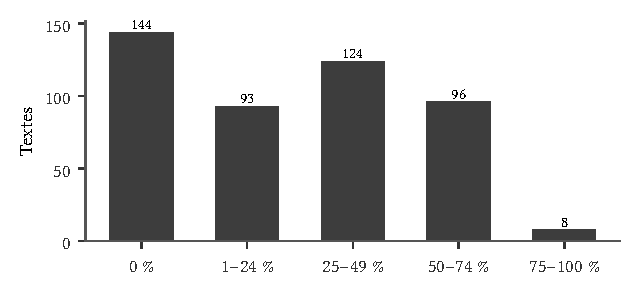
\includegraphics[width=0.7\linewidth]{figures/fig_restitution.pdf}
\caption{Part des lettres restituées déclarée par la base pour les textes de l’ensemble C (n = \st{nC}). Ces pourcentages ne mesurent pas la surface perdue des monuments.}\label{fig:restitution}
\end{figure}

La part des restitutions varie fortement d’un texte à l’autre (figure~\ref{fig:restitution}) : \st{nZeroRest} textes funéraires n’en comportent aucune, \st{nPlusMoitie} sont restitués pour plus de moitié. Pour ces derniers, toute observation linguistique ou religieuse est conditionnelle.

\section{Traductions}

Les traductions sont des traductions de travail. Elles suivent le texte au plus près ; les lacunes sont rendues par […], les sens incertains par un point d’interrogation entre parenthèses. Elles traduisent souvent des parties restituées par l’éditeur : le lecteur doit se reporter au texte pour distinguer ce qui est lu. Elles n’ont pas encore été relues par un spécialiste ; cette relecture, par un latiniste et un helléniste, est une condition de la publication.

\section{Structure des notices}

Chaque notice du catalogue suit le même ordre. Les rubriques sans objet sont omises.

\begin{description}[style=nextline,leftmargin=1.5em,font=\normalfont\scshape]
\item[En-tête] Numéro stable, année de classement, première référence ICUR, identifiants EDCS, EDB et, le cas échéant, EDH.
\item[Datation] Année et fondement : nom consulaire lu, lu en partie, réduit à des initiales ou restitué ; formule transmise par l’EDB ; restitution conjecturale ; attribution de la base. La mention « datation contestée » renvoie à la rubrique Chronologie.
\item[Genre] Genre épigraphique, appartenance aux ensembles B et C, nombre de lettres et part restituée.
\item[Références] Concordances transmises par l’EDCS, sous une forme normalisée. Elles n’ont pas été vérifiées sur les volumes.
\item[Provenance] Rattachement topographique et lieu de conservation selon l’EDB, cités dans la forme de la base.
\item[Support] Type de support, matériau, dimensions, technique d’exécution, signes figurés, caractère métrique et reproductions disponibles selon la fiche EpiDoc de l’EDB, avec le nom de son rédacteur.
\item[Texte] Texte de l’EDCS (état 2022), ligne par ligne.
\item[Témoins] Différences avec l’export de 2020 ; texte de l’EDB lorsqu’il diffère ; relecture des fiches détaillées ; décisions sur les doublons et les fragments.
\item[Apparat] Lettres gravées corrigées par l’éditeur, lettres superflues, formes signalées.
\item[Traduction] Traduction de travail.
\item[Langue, Chronologie, Commentaire] Observations linguistiques ; noms consulaires et leur état de lecture, faux consuls, dates du jour, âges, divergences ; vocabulaire religieux et renvoi au dossier commenté.
\item[Bibliographie] Références d’édition et bibliographie complémentaire donnée par l’EDB.
\item[Statut] Niveau de contrôle de la lecture.
\end{description}

Une épitaphe brève n’est pas artificiellement développée. Les dossiers commentés (chapitre~\ref{ch:dossiers}) complètent les notices dont les difficultés exigent une discussion.


\part{Datation et critique chronologique}
\chapter{Dater à Rome au IV\textsuperscript{e}~siècle}\label{ch:dater}

\section{Consulats et post-consulats}

La datation absolue des épitaphes du corpus repose presque exclusivement sur la mention des consuls ordinaires. Deux difficultés sont bien connues. Le nom des consuls de l’année pouvait n’être pas encore connu, ou pas reconnu, à Rome : on datait alors « après le consulat » des consuls précédents (\emph{post consulatum}). D’autre part, la proclamation des consuls dépendait de la situation politique : usurpations, consulats non reconnus dans une partie de l’Empire, condamnation de la mémoire d’un consul. L’instrument de référence pour ces questions est l’ouvrage de Bagnall, Cameron, Schwartz et Worp ; il est cité ici à travers les fiches de l’EDB lorsque celles-ci le reproduisent.

Le corpus illustre plusieurs de ces situations, et ses textes permettent d’en suivre les effets.

\emph{346.} Les quatre épitaphes classées en 346 datent par le post-consulat d’Amantius et Albinus (\nnums{15}–18). Le \nnum{15} associe une naissance datée par le consulat de Sabinus et Rufinus (316) et un décès « après le consulat d’Amantius et d’Albinus » : le calcul de la durée de vie confirme que ce post-consulat désigne bien 346 (chapitre~\ref{ch:calendrier}).

\emph{352–353.} Les consuls désignés sous l’usurpation de Magnence apparaissent en 352 (Décence et Paulus : \nnums{12}, 37–39) et, selon la lecture retenue, en 353 (Magnence et Décence : \nnum{40}). L’usage romain des consuls de Magnence est relevé par la recherche récente, qui note que la plupart des exemples datés de 352 remontent au printemps. Au \nnum{40}, la formule \emph{M⸢a⸣nnentio et Decen[ti]o} est interprétée par l’EDB, d’après la CLRE, comme une formule de 352 mal combinée par le lapicide ; la datation est déclarée contestée (chapitre~\ref{ch:fondement}). Le \nnum{12} porte deux formules consulaires : \emph{Amantio et Albino} (345), qui date un événement antérieur non précisé, et \emph{[Decentio et P]aulo} (352), rattachée à la déposition ; seule la fin du nom de Paulus est lue.

\emph{363.} Les dix épitaphes de 363 (\nnums{73}–82) datent par le quatrième consulat de Julien, avec Sallustius. Plusieurs sont postérieures à la mort de l’empereur, survenue en juin : le \nnum{81} est daté de décembre. Le consulat datait l’année, quel que fût le sort de l’empereur.

\emph{375.} Les dix textes du corpus classés en 375 (\nnums{179}–188) datent par le post-consulat de Gratien III et d’Equitius, ce qui concorde avec l’absence de nouveau collège dans la tradition des fastes (point à contrôler sur la CLRE). Au \nnum{180}, la formule n’est transmise que par l’EDB.

\emph{388.} Les textes datent soit par le consulat de l’usurpateur Magnus Maximus (\nnums{295}–297, 300, 302 et 311), soit par Théodose et Merobaudes. Au \nnum{298}, Merobaudes est dit consul pour la troisième fois (\emph{Merobaude v(iro) c(larissimo) III}, lu) ; au \nnum{303}, pour la deuxième. L’existence d’un troisième consulat de Merobaudes en 388 pose un problème prosopographique que la PLRE et la CLRE discutent, et qui n’a pas pu être contrôlé ici.

\emph{393.} Les épitaphes datent par Théodose et l’usurpateur Eugène (\nnums{351}–361). Le \nnum{351} porte en toutes lettres \emph{Theodosio III et Eugenio Augg(ustis)} ; le \nnum{360} transpose la formule en grec (\emph{Θεοδοσίῳ τό […]}).

\emph{394.} Le corpus atteste à la fois le consulat de Virius Nicomachus Flavianus, reconnu seulement dans le territoire d’Eugène\footnote{J. J. O’Donnell, « The Career of Virius Nicomachus Flavianus », \emph{Phoenix}, 32/2, 1978, p. 129–143, DOI 10.2307/1087470 (métadonnées vérifiées). Au \nnum{362}, le nom est en grande partie restitué : seul \emph{-abiani(!) v(iri)} est lu.} (\nnums{362}, 364–366), et le collège oriental d’Arcadius III et Honorius II (\nnums{363} et 367).

\emph{399.} Seul Mallius Theodorus est nommé (\nnums{429}, 430, 432, 433, 436–438), le consulat oriental de l’eunuque Eutrope n’ayant pas été reconnu en Occident. Au \nnum{435}, le nom n’est qu’une restitution de l’EDB ; au \nnum{431}, la formule \emph{post consulatu … Arcadi IIII et Eutychiani} (avec \emph{Harchadi} gravé pour \emph{Honorii}) est attribuée par la CLRE à 398.

\emph{400.} Stilichon est seul nommé (\nnums{439}–446). Au \nnum{444}, le groupe \emph{[iter(um) con]sule} est restitué par l’éditeur ; s’il était exact, il désignerait le second consulat de Stilichon (405). L’année 400 est conservée sous réserve. Au \nnum{445}, l’EDB restitue \emph{[iterum?]} avec doute.

\section{Table des consulats}

La table~\ref{tab:fastes} donne, pour chaque année, le collège consulaire selon la tradition des fastes et le nombre de textes de l’ensemble B classés sous cette année. Elle a servi à l’identification des consuls. Elle n’a pas été collationnée sur la CLRE et doit l’être avant publication ; les points litigieux sont signalés au chapitre suivant.

% généré par scripts/04_generated.py
\begin{longtable}{@{}r p{0.70\linewidth} r@{}}
\caption{Collèges consulaires 340–403 selon la tradition des fastes et nombre de textes distincts (ensemble B) classés sous chaque année. Table non collationnée sur la CLRE.}\label{tab:fastes}\\
\toprule Année & Collège consulaire & Textes\\\midrule\endfirsthead
\toprule Année & Collège consulaire & Textes\\\midrule\endhead
\bottomrule\endfoot
340 & Acindynus et Proculus & 3 \\
341 & Marcellinus et Probinus & 1 \\
342 & Constantius Aug. III et Constans Aug. II & 2 \\
343 & Placidus et Romulus & 3 \\
344 & Leontius et Sallustius & 1 \\
345 & Amantius et Albinus & 3 \\
346 & Constantius Aug. IV et Constans Aug. III (à Rome : p.c. Amantii et Albini) & 4 \\
347 & Rufinus et Eusebius & 3 \\
348 & Philippus et Salia & 8 \\
349 & Limenius et Catullinus & 4 \\
350 & Sergius et Nigrinianus & 2 \\
351 & Occident (Magnence) : Magnentius Aug. et Gaiso ; Orient : p.c. Sergii et Nigriniani & 1 \\
352 & Occident (Magnence) : Decentius Caes. et Paulus ; Constance : Constantius Aug. V et Constantius Caes. & 4 \\
353 & Occident (Magnence) : Magnentius Aug. II et Decentius Caes. II ; Constance : Constantius Aug. VI et Constantius Caes. II & 1 \\
354 & Constantius Aug. VII et Constantius Caes. III & 0 \\
355 & Arbitio et Lollianus & 4 \\
356 & Constantius Aug. VIII et Iulianus Caes. & 2 \\
357 & Constantius Aug. IX et Iulianus Caes. II & 2 \\
358 & Datianus et Cerealis & 5 \\
359 & Eusebius et Hypatius & 2 \\
360 & Constantius Aug. X et Iulianus Caes. III & 3 \\
361 & Taurus et Florentius & 3 \\
362 & Mamertinus et Nevitta & 11 \\
363 & Iulianus Aug. IV et Sallustius & 10 \\
364 & Iovianus Aug. et Varronianus & 9 \\
365 & Valentinianus Aug. et Valens Aug. & 6 \\
366 & Gratianus nob. puer et Dagalaifus & 7 \\
367 & Lupicinus et Iovinus & 18 \\
368 & Valentinianus Aug. II et Valens Aug. II & 7 \\
369 & Valentinianus nob. puer et Victor & 4 \\
370 & Valentinianus Aug. III et Valens Aug. III & 8 \\
371 & Gratianus Aug. II et Probus & 12 \\
372 & Modestus et Arintheus & 11 \\
373 & Valentinianus Aug. IV et Valens Aug. IV & 6 \\
374 & Gratianus Aug. III et Equitius & 7 \\
375 & Pas de consuls ordinaires : p.c. Gratiani III et Equitii & 10 \\
376 & Valens Aug. V et Valentinianus iun. Aug. & 6 \\
377 & Gratianus Aug. IV et Merobaudes & 11 \\
378 & Valens Aug. VI et Valentinianus iun. Aug. II & 3 \\
379 & Ausonius et Olybrius & 3 \\
380 & Gratianus Aug. V et Theodosius Aug. & 6 \\
381 & Syagrius et Eucherius & 10 \\
382 & Antonius et Syagrius & 13 \\
383 & Merobaudes II et Saturninus & 20 \\
384 & Richomeres et Clearchus & 15 \\
385 & Arcadius Aug. et Bauto & 6 \\
386 & Honorius nob. puer et Euodius & 8 \\
387 & Valentinianus Aug. III et Eutropius & 4 \\
388 & Theodosius Aug. II et Cynegius (Occident : Magnus Maximus Aug. II) ; Merobaudes III attesté par l'épigraphie (n° 298) & 10 \\
389 & Timasius et Promotus & 13 \\
390 & Valentinianus Aug. IV et Neoterius & 10 \\
391 & Tatianus et Symmachus & 13 \\
392 & Arcadius Aug. II et Rufinus & 8 \\
393 & Theodosius Aug. III et Abundantius ; à Rome : Eugenius Aug. & 11 \\
394 & Arcadius Aug. III et Honorius Aug. II ; territoire d'Eugène : Nicomachus Flavianus & 6 \\
395 & Olybrius et Probinus & 17 \\
396 & Arcadius Aug. IV et Honorius Aug. III & 10 \\
397 & Caesarius et Atticus & 22 \\
398 & Honorius Aug. IV et Eutychianus & 12 \\
399 & Mallius Theodorus et Eutropius (Occident : Theodorus seul) & 9 \\
400 & Stilicho et Aurelianus & 8 \\
401 & Vincentius et Fravitta & 13 \\
402 & Arcadius Aug. V et Honorius Aug. V & 9 \\
403 & Theodosius iun. Aug. et Rumoridus & 10 \\
\end{longtable}


\section{Le calendrier romain et la conversion des dates}

Les quantièmes sont exprimés selon le calendrier romain, par décompte inclusif à partir des calendes (le 1\textsuperscript{er} du mois), des nones (le 5, ou le 7 en mars, mai, juillet et octobre) et des ides (le 13, ou le 15 les mêmes mois). « Le 15\textsuperscript{e} jour avant les calendes d’avril » désigne le 18 mars. En année bissextile julienne, le 6\textsuperscript{e} jour avant les calendes de mars est redoublé ; la conversion en tient compte. Les dates sont converties dans le calendrier julien.

\begin{table}[tbp]\centering\small
\caption{Le calendrier romain (année ordinaire). Décompte inclusif : \emph{a.d.} N \emph{Kal.} = premier jour du mois suivant moins (N − 1) jours.}\label{tab:calendrier}
\begin{tabular}{@{}l r r r l@{}}\toprule Mois & Kal. & Non. & Id. & Jours suivant les ides\\\midrule
Janvier & 1 & 5 & 13 & 14 = \emph{a.d.} XIX \emph{Kal. Febr.} … 31 = \emph{prid. Kal. Febr.}\\
Février & 1 & 5 & 13 & 14 = \emph{a.d.} XVI \emph{Kal. Mart.} … 28 = \emph{prid. Kal. Mart.}\\
Mars & 1 & 7 & 15 & 16 = \emph{a.d.} XVII \emph{Kal. Apr.} … 31 = \emph{prid. Kal. Apr.}\\
Avril & 1 & 5 & 13 & 14 = \emph{a.d.} XVIII \emph{Kal. Mai.} … 30 = \emph{prid. Kal. Mai.}\\
Mai & 1 & 7 & 15 & 16 = \emph{a.d.} XVII \emph{Kal. Iun.} … 31 = \emph{prid. Kal. Iun.}\\
Juin & 1 & 5 & 13 & 14 = \emph{a.d.} XVIII \emph{Kal. Iul.} … 30 = \emph{prid. Kal. Iul.}\\
Juillet & 1 & 7 & 15 & 16 = \emph{a.d.} XVII \emph{Kal. Aug.} … 31 = \emph{prid. Kal. Aug.}\\
Août & 1 & 5 & 13 & 14 = \emph{a.d.} XIX \emph{Kal. Sept.} … 31 = \emph{prid. Kal. Sept.}\\
Septembre & 1 & 5 & 13 & 14 = \emph{a.d.} XVIII \emph{Kal. Oct.} … 30 = \emph{prid. Kal. Oct.}\\
Octobre & 1 & 7 & 15 & 16 = \emph{a.d.} XVII \emph{Kal. Nov.} … 31 = \emph{prid. Kal. Nov.}\\
Novembre & 1 & 5 & 13 & 14 = \emph{a.d.} XVIII \emph{Kal. Dec.} … 30 = \emph{prid. Kal. Dec.}\\
Décembre & 1 & 5 & 13 & 14 = \emph{a.d.} XIX \emph{Kal. Ian.} … 31 = \emph{prid. Kal. Ian.}\\\bottomrule
\end{tabular}
\end{table}

\section{Jours de la semaine et âge de la lune}

Quelques textes indiquent le jour de la semaine selon la nomenclature planétaire (\emph{dies Solis, Lunae, Martis, Mercurii, Iovis, Veneris, Saturni}) et, plus rarement, l’âge de la lune. Le jour de la semaine est vérifié par le calcul du jour julien dans le calendrier julien. L’âge de la lune et sa position dans le zodiaque sont calculés avec la bibliothèque d’éphémérides PyEphem (version 4.2.1), dont on a vérifié qu’elle emploie le calendrier julien pour ces dates : le jour julien calculé pour le 23 août 386 coïncide avec celui de l’algorithme de conversion, soit 1\,862\,279. Ces contrôles font l’objet du chapitre~\ref{ch:calendrier}.

\chapter{Le fondement des années}\label{ch:fondement}

Une année de classement n’est pas une date établie. Ce chapitre rapporte chaque année à ce qui la fonde dans le texte transmis, en distinguant les lettres lues, les lettres restituées par l’éditeur et les données qui proviennent de la seule base de données.

\section{Année de la base, année du texte, année de classement}

La base de travail distingue, pour chaque notice, l’année fournie par l’EDCS, l’année déduite du texte lorsque les consuls nommés la déterminent, et l’année retenue pour le classement, accompagnée d’une justification. L’année de classement est celle de la base, sauf lorsque le texte la contredit de manière univoque. Sept notices sont dans ce cas (tableau~\ref{tab:correctionsbase}) ; l’année de la base reste consultable dans les données. Pour quatre d’entre elles, la confrontation avec l’EDB a fait apparaître une autre lecture possible : la correction est maintenue, mais la datation est déclarée contestée.

\begin{table}[tbp]\centering\small
\caption{Années de la base corrigées d’après le texte.}\label{tab:correctionsbase}
\begin{tabularx}{\linewidth}{@{}r r r X@{}}\toprule
N° & Base & Classement & Justification et état actuel\\\midrule
12 & 345 & 352 & Deux formules consulaires ; \emph{-aulo conss.} est lu et Paulus n’est consul qu’en 352 ; \emph{Amantio et Albino} (345) date un événement antérieur non précisé.\\
206 & 377 & 370 & \emph{Valentiniano III et Valente Augg.} ne convient qu’à 370 ; l’EDB date aussi de 377, vraisemblablement par erreur de saisie.\\
278 & 385 & 383 & \emph{Merobaude II et Saturnino} = 383 ; l’EDB date de 385, mais date de 383 une fiche voisine du même consulat.\\
311 & 389 & 388 & \emph{Maximo cons(ule)} : consulat de Magnus Maximus (388). L’EDB date de 389 : contestée.\\
314 & 389 & 390 & Formule \emph{Valentiniano Aug. IIII et Neoterio} (390), entièrement restituée sauf \emph{d(omino) n(ostro) V}. Contestée.\\
328 & 390 & 381 & Seul \emph{…terio} est lu : Eucherius (381) ou Neoterius (390). Contestée.\\
434 & 399 & 397 & \emph{p(ost) cons(ulatum) Arcadi I[II]I} = 397 ; l’EDB date de 399.\\\bottomrule
\end{tabularx}
\end{table}

Deux autres cas relèvent du calcul interne. Au \nnum{19}, Lea est morte sous Amantius et Albinus (345) ; l’année 347 de la base paraît déduite d’une indication « il y a deux ans » que l’EDCS restitue et que l’EDB ne retient pas : le texte est daté au plus tôt de 345. Au \nnum{55}, la discordance apparente se résout par le calcul : le défunt est né sous Acindynus et Proculus (340), le 21 juin ; 19 ans, 3 mois et 6 jours plus tard, on parvient au 27 septembre 359, qui est exactement le 5\textsuperscript{e} jour avant les calendes d’octobre gravé comme date de déposition.

\section{Lire, restituer : quatre niveaux pour le nom consulaire}

L’identification d’un collège consulaire ne dit pas, à elle seule, ce qui en est lu. La formule \emph{[Acin]dino et Procu[lo conss(ulibus)]} permet d’identifier l’année 340, mais les deux noms n’y sont conservés qu’en partie. Pour chaque texte à datation directe, l’état de lecture de chaque nom consulaire a donc été relevé sur la transcription, puis classé selon le meilleur nom :

\begin{description}[style=nextline,leftmargin=1.5em,font=\normalfont\scshape]
\item[A — nom lu] au moins un nom consulaire est entièrement lu ;
\item[B — lecture partielle] au moins trois lettres gravées d’un nom sont lues, le reste étant restitué ;
\item[C — initiales] les noms sont réduits à des initiales (\emph{M(amertino) et N(evitta)}, \nnum{70}) ;
\item[R — consulat restitué] aucun nom n’atteint le niveau B : l’année repose sur une restitution de l’éditeur, guidée par des lettres isolées, une itération ou le contexte.
\end{description}

Dans l’ensemble C, l’année de \st{datLu} textes repose sur un nom consulaire lu, celle de \st{datPartiel} sur une lecture partielle, celle de \st{datInit} sur des initiales et celle de \st{datRest} sur un consulat restitué (tableau~\ref{tab:datation}, figure~\ref{fig:annees}). Le niveau R ne signifie pas que l’année est fausse : la restitution est souvent contrainte par une itération ou une titulature. Il signifie qu’elle ne peut pas servir de jalon indépendant pour dater d’autres textes.

% généré par scripts/04_generated.py
\begin{table}[tbp]\centering\small\caption{Fondement de l’année dans l’ensemble C (n = 465). Les listes de plus de quarante notices sont données dans la chronique (chapitre~\ref{ch:chronique}).}\label{tab:datation}
\begin{tabular}{@{}p{0.36\linewidth} r p{0.5\linewidth}@{}}\toprule Fondement & Textes & Notices\\\midrule
Directe : nom consulaire lu & 330 & {\footnotesize —} \\
Directe : lecture partielle d’un nom consulaire & 96 & {\footnotesize —} \\
Directe : initiales consulaires & 2 & {\footnotesize 48, 70} \\
Directe : consulat restitué & 21 & {\footnotesize 52, 129, 137, 138, 161, 203, 219, 222, 256, 290, 314, 384, 393, 415, 426, 432, 438, 452, 455, 465, 468} \\
Formule transmise par l’EDB (lue) & 4 & {\footnotesize 84, 214, 268, 388} \\
Formule transmise par l’EDB (lue, itération restituée) & 1 & {\footnotesize 445} \\
Formule transmise par l’EDB (partiellement restituée) & 3 & {\footnotesize 51, 180, 447} \\
Conjecturale & 4 & {\footnotesize 123, 326, 435, 457} \\
Indirecte & 4 & {\footnotesize 36, 267, 348, 349} \\
\bottomrule\end{tabular}\end{table}


\begin{figure}[tbp]\centering
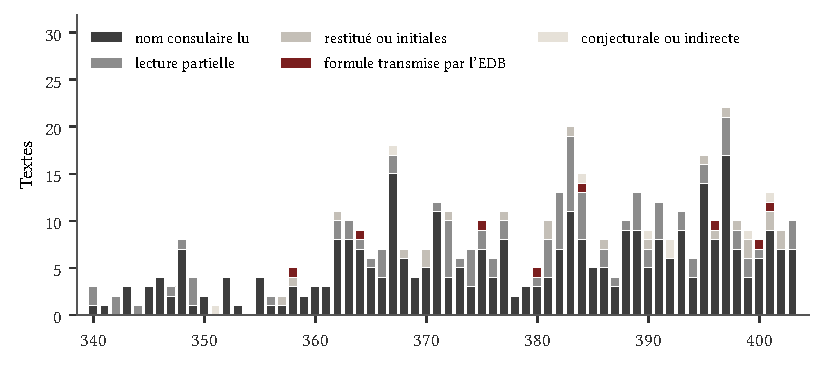
\includegraphics[width=\linewidth]{figures/fig_annees.pdf}
\caption{Textes de l’ensemble C par année de classement et par fondement de l’année.}\label{fig:annees}
\end{figure}

\section{Huit formules transmises par la seule EDB}

Pour seize notices du catalogue initial, le texte EDCS ne conservait aucun élément consulaire, et l’année provenait de la base. La confrontation avec l’EDB modifie ce constat pour huit d’entre elles, dont la formule de date est transmise par la seconde base :

\begin{itemize}
\item formule lue : \nnums{84} (Jovien et Varronianus, 364), 214 (Gratien V et Théodose, 380), 268 (Richomer et Clearchus, 384), 388 (Arcadius IV et Honorius III, 396) ;
\item formule lue, itération restituée : \nnum{445} (\emph{Stellici v(iri) c(larissimi) [iterum?]}, 400, ou 405 si \emph{iterum} est retenu) ;
\item formule partiellement restituée : \nnums{51} (Cerealis, 358), 180 (post-consulat d’Equitius, 375), 447 (Fravitta, 401).
\end{itemize}

Quatre autres notices reçoivent de l’EDB une restitution conjecturale (\nnums{123}, 326, 435 et 457). Au \nnum{123}, les deux lectures sont incompatibles : là où l’EDB restitue \emph{[Lupicin?]o et ⟨I⟩ovi[no]}, l’EDCS lit \emph{[- - -]o et o⸢b⸣i[it]}, « et mourut ». Ces quatre textes sont classés « conjecturaux ». Restent quatre textes dont l’année provient de la seule base, sans formule consulaire dans aucun témoin : \nnums{36} (datation prosopographique), 267 (fragment), 348 (épitaphe grecque d’Alexandros) et 349 (épitaphe de Leoparda, dont le jour de la semaine et l’âge de la lune sont compatibles avec 392 ; chapitre~\ref{ch:calendrier}).

\section{Faux consuls}

L’identification automatique des consuls, qui rapproche les noms du texte d’une liste de consuls, a produit des erreurs de rôle : \st{nFauxConsuls} noms, dans \st{nFauxConsulsNotices} notices, désignent en réalité un défunt, un dédicant, une personne citée ou un fonctionnaire. Ainsi, au \nnum{68}, \emph{Eutyches pater fecit} nomme le père qui commémore, non le consul Eutychianus de 398 ; au \nnum{55}, \emph{Marcellinus} est le défunt ; au \nnum{321}, \emph{Fl(avius) Filippus} est le responsable des travaux de la colonne de Saint-Paul et \emph{Paul(us)} l’apôtre ; au \nnum{462}, \emph{Saturninus} est le défunt. Aucune de ces erreurs ne modifie l’année de classement, qui repose dans tous les cas sur l’autre consul ou sur le collège complet. Les rôles corrects sont donnés dans chaque notice (rubrique Chronologie) et dans l’index des consuls.

\section{Datations contestées et réserves}

Dix datations sont contestées : deux lectures publiées, ou deux restitutions également possibles, conduisent à deux années différentes. Cinq autres font l’objet d’une réserve : la formule transmise ne concorde pas entièrement avec le collège de l’année de classement. Deux divergences, enfin, sont vraisemblablement des erreurs de saisie de l’EDB. Le tableau~\ref{tab:contestees} donne les motifs. Dans tous les cas, l’année de classement est conservée : aucune année n’est modifiée par vraisemblance.

% généré par scripts/04_generated.py
\begin{longtable}{@{}r r l p{0.6\linewidth}@{}}\caption{Datations contestées, réserves et divergences attribuées à l’EDB. L’année de classement est conservée dans tous les cas.}\label{tab:contestees}\\\toprule N° & Année & Statut & Motif\\\midrule\endfirsthead\toprule N° & Année & Statut & Motif\\\midrule\endhead\bottomrule\endfoot
40 & 353 & contestée & {\footnotesize Magnence III et Décence II (353) selon la lecture retenue ; l’EDB, citant CLRE p. 636, date de 352 en supposant une erreur du lapicide.} \\
52 & 358 & contestée & {\footnotesize Da[tiano] (358) selon Silvagni ; la CLRE (p. 631, citée par l’EDB) rappelle que Dalmatius, consul en 333, commence aussi par DA. Si 333, la notice sort du corpus.} \\
141 & 370 & contestée & {\footnotesize Valentinien III : Valentinien Ier (370) ou Valentinien II (387) ; la CLRE (p. 644, citée par l’EDB) note « Year doubtful: 387 possible ».} \\
165 & 372 & contestée & {\footnotesize L’année 372 repose sur la seule séquence « dest », interprétée par Ferrua comme [Mo]dest[o] ; l’EDB date « 300-399 ».} \\
206 & 370 & EDB fautive & {\footnotesize L’EDB date de 377 ; la formule Valentiniano III et Valente Augg. ne convient qu’à 370 : erreur probable de saisie de l’EDB.} \\
220 & 381 & contestée & {\footnotesize Seul …erio est lu ; l’EDB signale d’autres restitutions possibles (Val]erio, Gal]erio, Neot]erio, Ast]erio) : 381 ou 390.} \\
278 & 383 & EDB fautive & {\footnotesize L’EDB date de 385 ; Merobaude II et Saturnino = 383, et la fiche voisine EDB8750 (même consulat) est datée de 383 : incohérence interne probable de l’EDB.} \\
311 & 388 & contestée & {\footnotesize Maximo cons(ule) : consulat de Magnus Maximus (388) ; l’EDB date de 389 et signale une transcription différente de l’ICVR.} \\
314 & 390 & contestée & {\footnotesize Second texte du monument ICUR IV 11117 : seul d(omino) n(ostro) V[…] est lu ; 390 est une restitution partagée par l’EDCS et l’EDB, que la note de l’EDB juge contradictoire avec l’ordre des décès.} \\
328 & 381 & contestée & {\footnotesize Seul …terio est lu : Eucherio (381) ou Neoterio (390).} \\
395 & 396 & réserve & {\footnotesize Itération d’Honorius (IIII transmis) à confronter au collège de 396 (Arcadius IV et Honorius III).} \\
411 & 397 & réserve & {\footnotesize Collège Caesarius et Maximus ; les fastes donnent pour 397 Caesarius et Atticus.} \\
428 & 398 & réserve & {\footnotesize Post-consulat d’Honorius IV et Eutychianus (399 ?) ou consulat (398) ; le jour de la semaine (samedi) convient au 18 décembre 398.} \\
431 & 399 & contestée & {\footnotesize La CLRE (p. 661, citée par l’EDB) attribue le texte à 398 ; 399 suppose un post restitué que l’EDB juge trop long.} \\
434 & 397 & contestée & {\footnotesize Post-consulat d’Arcadius IV : 397 ; l’EDB date de 399.} \\
444 & 400 & réserve & {\footnotesize Itération [iter(um)] de Stilichon restituée ; compatibilité avec 400 à contrôler.} \\
466 & 402 & réserve & {\footnotesize Paire Arcadius–Théodose à contrôler sur les fastes de 402.} \\
\end{longtable}


\section{Distribution chronologique}

La distribution des textes funéraires par année de classement est très inégale (figure~\ref{fig:annees}). Elle progresse nettement à partir de 360, et \st{partApres380}~\% des textes de l’ensemble C appartiennent aux années 380–403. Les périodes utilisées dans la suite du livre comptent \st{perC0} textes (340–359), \st{perC1} (360–374), \st{perC2} (375–389) et \st{perC3} (390–403). Cette progression peut traduire une diffusion de la datation consulaire dans les épitaphes chrétiennes ; elle peut aussi tenir aux hasards de la conservation et de la publication. Le corpus ne permet pas de trancher entre ces explications.

\chapter{Contrôles calendaires et astronomiques}\label{ch:calendrier}

\section{Les dates du jour}

Dans l’ensemble C, \st{nTextesDate} textes contiennent au moins une date convertible en date julienne ; on compte au total \st{nDatesConv} dates converties. Le terme qui précède l’expression calendaire permet d’identifier l’événement daté dans la plupart des cas : déposition (\st{ev_depo}), décès (\st{ev_deces}), naissance (\st{ev_naiss}), achat (\st{ev_achat}) ; \st{ev_indet} dates restent rattachées à un événement indéterminé. Ces nombres comptent des dates, non des textes : un même document peut en contenir plusieurs.

La répartition mensuelle de la première date de chaque texte (figure~\ref{fig:mois}) présente un excédent estival : \st{ete}~\% de ces dates tombent en juillet, août ou septembre. Un test d’ajustement du χ² à une répartition proportionnelle à la longueur des mois donne χ² = \st{chi2} pour onze degrés de liberté (\emph{p} ≈ \st{chi2p}) : l’écart n’atteint pas le seuil conventionnel de 5~\%. L’observation est compatible avec la saisonnalité estivale décrite par Shaw sur un ensemble beaucoup plus large ; elle ne la démontre pas. Elle ne mesure pas non plus la mortalité : l’événement daté est le plus souvent la déposition, et la sélection des textes datés n’a rien d’aléatoire.

\begin{figure}[tbp]\centering
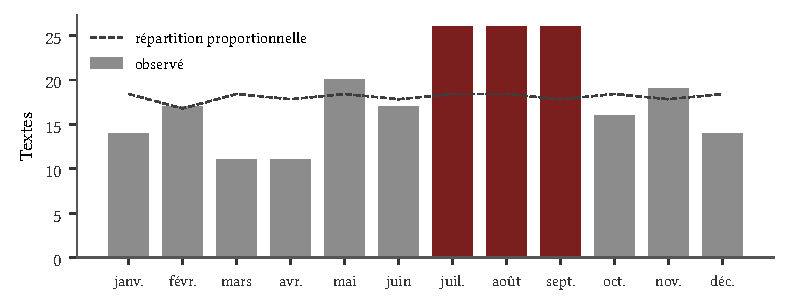
\includegraphics[width=0.9\linewidth]{figures/fig_mois.pdf}
\caption{Mois de la première date convertie de chaque texte de l’ensemble C (n = \st{nMoisTot}) ; trait discontinu : répartition proportionnelle à la longueur des mois.}\label{fig:mois}
\end{figure}

\section{Les jours de la semaine}

Le jour de la semaine est mentionné dix-huit fois dans seize textes. Le tableau~\ref{tab:jours} donne le résultat du contrôle par le calcul du jour julien ; pour les \nnums{55} et 126, la mention se rapporte à la naissance, et le calcul porte sur l’année de la naissance.

% généré par scripts/04_generated.py
\begin{table}[tbp]\centering\footnotesize\setlength{\tabcolsep}{3.5pt}\caption{Contrôle des jours de la semaine (calendrier julien, recalcul ; l’année est celle de l’événement daté : naissance pour les \nnums{55} et 126 première mention).}\label{tab:jours}
\begin{tabular}{@{}r r l l l l l@{}}\toprule N° & Année & Mention & Quantième & Date & Calcul & Résultat\\\midrule
7 & 343 & \lat{die Martis} & \lat{III Nonas Iulias} & 5/7/343 & mardi & concordant \\
55 & 340 & \lat{die Veneris} & \lat{XI Kalendas Iulias} & 21/6/340 & samedi & écart d’un jour \\
118 & 367 & \lat{die Martis} & \lat{—} & — & — & quantième lacunaire \\
122 & 367 & \lat{die Martis} & \lat{Nonis Iuniis} & 5/6/367 & mardi & concordant \\
126 & 350 & \lat{die Saturnis} & \lat{III Idus Augustas} & 11/8/350 & samedi & concordant \\
126 & 368 & \lat{die Saturnis} & \lat{VII Idus Decembres} & 7/12/368 & dimanche & écart d’un jour \\
128 & 368 & \lat{die Martis} & \lat{XV Kalendas Decembres} & 17/11/368 & lundi & écart d’un jour \\
131 & 368 & \lat{die Veneris} & \lat{pridie Nonas Martias} & 6/3/368 & jeudi & écart d’un jour \\
169 & 373 & \lat{die Lunae} & \lat{XV Kalendas Apriles} & 18/3/373 & lundi & concordant \\
275 & 385 & \lat{die Lunae} & \lat{VI Idus Martia} & 10/3/385 & lundi & concordant \\
287 & 386 & \lat{die Solis} & \lat{X Kalendas Septembres} & 23/8/386 & dimanche & concordant \\
349 & 392 & \lat{die Veneris} & \lat{XV Kalendas Octobres} & 17/9/392 & vendredi & concordant \\
381 & 395 & \lat{die Saturni} & \lat{III Idus Maias} & 13/5/395 & dimanche & écart d’un jour \\
381 & 395 & \lat{die Lunae} & \lat{XII Kalendas Iunias} & 21/5/395 & lundi & concordant \\
416 & 397 & \lat{die Veneris} & \lat{tertium Kalendas Iulias} & 29/6/397 & lundi & discordant \\
428 & 398 & \lat{die Saturni} & \lat{XV Kalendas Ianuarias} & 18/12/398 & samedi & concordant \\
428 & 399 & \lat{die Saturni} & \lat{XV Kalendas Ianuarias} & 18/12/399 & dimanche & écart d’un jour \\
431 & 399 & \lat{die Veneris} & \lat{septimum Kalendas Septembres} & 26/8/399 & vendredi & concordant \\
462 & 402 & \lat{die Saturni} & \lat{—} & — & — & quantième lacunaire \\
\bottomrule\end{tabular}\end{table}


Neuf mentions concordent avec la date convertie, et la mention du \nnum{428} concorde si l’on retient 398 plutôt que 399. Dans cinq cas (\nnums{55}, 126 seconde mention, 128, 131 et 381 première mention), l’écart est d’un jour, tantôt dans un sens, tantôt dans l’autre. Ces écarts peuvent tenir à la distinction entre décès et déposition, au rattachement d’un décès nocturne au jour précédent ou suivant, ou à une erreur de gravure ou de lecture ; le corpus ne permet pas de les départager. Au \nnum{416}, le vendredi gravé ne correspond pas au 29 juin 397, qui est un lundi ; l’expression \emph{post ter[tiu]m Kalendas Iulia[s]} est d’interprétation incertaine, et la conversion elle-même doit être tenue pour douteuse. Pour les \nnums{118} et 462, le quantième est perdu.

\section{Deux mentions de l’âge de la lune}

Le \nnum{287} associe un jour de la semaine (\emph{[di]e Sol⸢i⸣s}), un âge de la lune (\emph{[Lu]na XII}) et un signe zodiacal (\emph{[Capricor]nus}) à une date dont le quantième est entièrement restitué par l’éditeur (\emph{[X Kal(endas) Sept(embres)]}). L’année 386 est donnée par la formule consulaire, dont le nom d’Honorius est lu. Le calcul montre que la restitution est compatible avec les indications conservées : le 23 août 386 (julien) est un dimanche ; l’éphéméride donne pour ce jour un âge de la lune compris entre 11,5 jours (à minuit) et 12,5 jours (à 24~h) depuis la nouvelle lune du 11 août, et une longitude écliptique comprise entre 285,6° et 300,6°, dans le signe du Capricorne (270°–300°). Ce n’est pas une confirmation indépendante : si l’éditeur a restitué le quantième à partir de ces mêmes données, le raisonnement serait circulaire. Le fondement de la restitution doit être vérifié dans l’édition.

Le \nnum{349} date la mort de Leoparda du 15\textsuperscript{e} jour avant les calendes d’octobre (17 septembre), un vendredi, \emph{luna XV}. Ce texte ne contient aucun élément consulaire, ni dans l’EDCS ni dans l’EDB : son année (392) provient de la base. Le 17 septembre 392 est bien un vendredi, et l’âge de la lune est ce jour-là compris entre 13,5 et 14,5 jours (nouvelle lune du 3 septembre), ce qui correspond au quatorzième ou au quinzième jour de la lunaison selon le mode de décompte. Le jour de la semaine et l’âge de la lune fournissent ainsi un test de compatibilité avec l’année proposée, sans en démontrer à eux seuls l’unicité.

\section{Naissance, âge et décès}

Trois textes permettent de vérifier la cohérence entre une date de naissance, un âge et une date de décès.

Au \nnum{15}, Cassia, née le 15 juin 316 (consulat de Sabinus et Rufinus) et morte le 15 septembre 346, a vécu « 30 ans et 93 jours » : du 15 juin au 15 septembre on compte 92 jours, soit 93 en décompte inclusif. La durée gravée est donc exactement cohérente avec les deux dates, et le cas confirme que le post-consulat d’Amantius et Albinus désigne 346.

Au \nnum{55}, le calcul conduit de la naissance (21 juin 340) à la déposition (27 septembre 359), conformément au quantième gravé. Le jour de naissance est dit \emph{die Veneris} ; le calcul julien donne un samedi pour le 21 juin 340. L’écart d’un jour est conservé sans correction.

Au \nnum{126}, du 11 août 350 au 7 décembre 368, on compte 18 ans, 3 mois et 26 jours ; le texte donne 19 ans, 3 mois et 26 jours. Les mois et les jours concordent exactement, sans établir indépendamment la validité des deux dates, tandis que l’écart d’une année reste inexpliqué : décompte inclusif des années, erreur de gravure ou de lecture du chiffre \emph{XVIIII}.

\chapter{Que date la date ? Événements, séquences et gravure}\label{ch:evenements}

Une année consulaire n’est intelligible qu’avec l’événement auquel elle se rapporte. La mention d’une naissance ne date pas une mort ; l’achat d’un emplacement ne date pas la déposition ; une commémoration collective peut juxtaposer des événements éloignés. L’année de classement du catalogue est donc un instrument de repérage, non une variable historique immédiatement univoque.

\section{Identifier l’événement avant de classer la date}

Le relevé associe à chaque indication calendaire un événement, une personne lorsque celle-ci est identifiable, un statut textuel et une justification. Les verbes de décès (\emph{decessit, recessit, defunctus, quievit}) et les termes de déposition (\emph{depositus, depositio}) fournissent des indices distincts. L’association d’une date au mot le plus proche aide au repérage ; elle ne remplace pas l’analyse de la syntaxe et de la structure du document. En l’absence de relation explicite, la catégorie reste « événement indéterminé » : c’est le cas de \st{ev_indet} dates sur \st{nDatesConv} dans l’ensemble C.

\section{Décès et déposition}

Les \nnums{119} et 211 distinguent un décès et une mise au tombeau. Leur intérêt est d’attester que deux opérations peuvent recevoir deux dates dans le même document. Ils ne suffisent pas à fournir un délai habituel d’inhumation, ni à expliquer tous les écarts entre quantième et jour de la semaine. Un écart peut relever de la lecture, du calcul, d’une notation inclusive ou de la relation entre événements ; ces possibilités doivent rester distinctes tant qu’un témoin supplémentaire ne permet pas de décider.

\section{Documents à plusieurs indications chronologiques}

Les \nnums{15}, 55 et 126 obligent à séparer une naissance d’un événement funéraire. D’autres documents juxtaposent plusieurs défunts. La grande dalle du \nnum{134} (105 × 190 cm selon l’EDB) porte plusieurs textes : la \emph{dormitio} du prêtre Dulcitius, celle du diacre Gregorius et celle de leur sœur, puis la déposition de Faustina, datée par le consulat de Valentinien \emph{nobilissimus puer} et de Victor (369), et la \emph{dormitio} d’Agapè. L’EDB date l’ensemble « 350–399 ; 369 » : l’année de classement n’est portée que par l’une des parties, et les autres dates ne sont pas nécessairement de la même année. La plaque ICUR IV 11117 porte de même deux dépositions successives, d’un défunt en 389 (\nnum{313}) et de son frère (\nnum{314}), dont l’année est restituée. Les \nnums{117}, 236, 317 et 373 demandent une analyse semblable de la succession des commémorations. L’attribution de chaque date à un défunt ou à une intervention doit être contrôlée dans la notice, sans la déduire du seul nombre de consulats.

Pour les analyses du volume, la règle de classement reste l’année retenue dans le catalogue. Cette variable est expressément nommée « année de classement ». Une analyse de la mort doit employer les événements de décès ; une analyse des dépositions, les événements de déposition. Une étude de la production épigraphique doit distinguer les phases de gravure et ne peut prendre automatiquement la première ou la dernière date funéraire pour l’année de fabrication du support.

\section{Préparation du vivant et additions}

Une formule \emph{se vivo}, \emph{se viva} ou \emph{se vivi} signale une initiative prise du vivant d’un commanditaire. Elle ne garantit pas que toute la surface conservée a été gravée au même moment. Le \nnum{300} associe ainsi une préparation du vivant et une mention de décès ; l’ordre exact des opérations ne peut être établi sur la seule continuité du texte transmis.

La date du dernier événement mentionné fournit au plus tôt une limite pour l’état complet du texte, sous réserve de l’interprétation des événements et de l’absence d’addition postérieure. Elle ne suffit pas à dater toutes les lignes ni le premier emploi du support. La matérialité de l’inscription est ici une condition de l’analyse chronologique, non un complément décoratif.

\section{Quand la date n’appartient qu’à un témoin}

La confrontation des bases ajoute un cas de figure. Pour huit textes, la formule de date n’est transmise que par l’EDB (chapitre~\ref{ch:fondement}). Inversement, au \nnum{378}, la formule \emph{[Olybrio et Pro]bino} (395) et la généalogie cléricale qui l’accompagne ne figurent dans aucune des fiches EDB que l’on peut rattacher au monument (ICVR III 8345, 8274c et 8387v) : l’EDB date l’ensemble « 390–424 ». L’année de classement repose alors sur une partie du texte qu’un seul témoin transmet. Elle est conservée, mais elle ne peut servir de jalon tant que l’ICVR III 8345 n’a pas été contrôlée.

\section{Faces, champs et remploi}

Une rupture de champ dans un export n’est pas une preuve de remploi. Elle peut représenter deux faces, deux zones d’une même plaque, une addition ou une convention de saisie. Les fiches de l’EDB précisent parfois la disposition : la colonne de Saint-Paul (\nnum{321}) porte trois textes en trois endroits du fût ; la dalle du \nnum{134} a été remployée en morceaux dans un mur. Ailleurs, la qualification d’un support comme opisthographe ou remployé exige une édition descriptive, une photographie ou un examen matériel.

\chapter{Chronique consulaire du corpus, 340–403}\label{ch:chronique}

Ce chapitre présente, année par année, les textes de l’ensemble B classés sous chaque année, avec le collège consulaire selon la tradition des fastes (table~\ref{tab:fastes}). Pour chaque texte sont indiqués le fondement de l’année et, pour les noms consulaires, leur état de lecture : \emph{lu}, \emph{partiel} (au moins trois lettres lues, le reste restitué) ou \emph{restitué}. Les mentions « contestée » et « réserve » renvoient au tableau~\ref{tab:contestees}. L’objectif est double : rendre contrôlable l’attribution de chaque texte à son année, et documenter la variété des formules de datation, qui est elle-même un objet d’étude. Le détail des formules se lit dans les notices.

% généré par scripts/04_generated.py
\chronan{340}{Acindynus et Proculus}{\nnum{1} Acindynus (lu), Proculus (restitué) \textbullet{} \nnum{2} Acindynus (partiel), Proculus (partiel) \textbullet{} \nnum{3} Acindynus (partiel), Proculus (restitué)}
\chronan{341}{Marcellinus et Probinus}{\nnum{4} Marcellinus (lu), Probinus (lu)}
\chronan{342}{Constantius Aug. III et Constans Aug. II}{\nnum{5} Constantius (partiel), Constans (partiel) \textbullet{} \nnum{6} Constantius (partiel), Constans (restitué)}
\chronan{343}{Placidus et Romulus}{\nnum{7} Placidus (lu), Romulus (lu) \textbullet{} \nnum{8} Romulus (lu); grec \textbullet{} \nnum{9} Placidus (lu), Romulus (lu)}
\chronan{344}{Leontius et Sallustius}{\nnum{10} Leontius (restitué), Sallustius (absent)}
\chronan{345}{Amantius et Albinus}{\nnum{11} Amantius (lu), Albinus (restitué) \textbullet{} \nnum{13} Amantius (lu), Albinus (restitué) \textbullet{} \nnum{14} Amantius (lu), Albinus (restitué)}
\chronan{346}{Constantius Aug. IV et Constans Aug. III (à Rome : p.c. Amantii et Albini)}{\nnum{15} Amantius (lu), Albinus (restitué), Rufinus (lu); post-consulat \textbullet{} \nnum{16} Amantius (lu), Albinus (lu); post-consulat \textbullet{} \nnum{17} Amantius (lu), Albinus (lu); post-consulat \textbullet{} \nnum{18} Amantius (partiel), Albinus (lu); post-consulat}
\chronan{347}{Rufinus et Eusebius}{\nnum{19} Amantius (lu), Albinus (lu) \textbullet{} \nnum{20} Rufinus (lu), Eusebius (restitué) \textbullet{} \nnum{21} Rufinus (restitué), Eusebius (partiel); grec}
\chronan{348}{Philippus et Salia}{\nnum{22} Philippus (lu) \textbullet{} \nnum{23} Philippus (lu), Salia (lu) \textbullet{} \nnum{24} Philippus (lu), Salia (restitué) \textbullet{} \nnum{25} Philippus (partiel), Salia (restitué) \textbullet{} \nnum{26} Philippus (lu), Salia (lu) \textbullet{} \nnum{27} Philippus (lu), Salia (lu) \textbullet{} \nnum{28} Philippus (restitué), Salia (lu) \textbullet{} \nnum{29} Philippus (lu), Salia (lu)}
\chronan{349}{Limenius et Catullinus}{\nnum{30} Limenius (partiel), Catullinus (restitué) \textbullet{} \nnum{31} Limenius (restitué), Catullinus (partiel) \textbullet{} \nnum{32} Limenius (partiel), Catullinus (partiel) \textbullet{} \nnum{33} Limenius (lu), Catullinus (lu)}
\chronan{350}{Sergius et Nigrinianus}{\nnum{34} Limenius (lu), Catullinus (lu); post-consulat \textbullet{} \nnum{35} Nigrinianus (lu)}
\chronan{351}{Occident (Magnence) : Magnentius Aug. et Gaiso ; Orient : p.c. Sergii et Nigriniani}{\nnum{36} aucun élément consulaire}
\chronan{352}{Occident (Magnence) : Decentius Caes. et Paulus ; Constance : Constantius Aug. V et Constantius Caes.}{\nnum{12} Amantius (lu), Albinus (lu), Decentius (restitué), Paulus (partiel) \textbullet{} \nnum{37} Decentius (lu), Paulus (lu) \textbullet{} \nnum{38} Decentius (lu), Paulus (lu) \textbullet{} \nnum{39} Decentius (restitué), Paulus (lu)}
\chronan{353}{Occident (Magnence) : Magnentius Aug. II et Decentius Caes. II ; Constance : Constantius Aug. VI et Constantius Caes. II}{\nnum{40} Magnentius (lu), Decentius (partiel); \textit{contestée}}
\chronan{354}{Constantius Aug. VII et Constantius Caes. III}{Aucun texte du corpus.}
\chronan{355}{Arbitio et Lollianus}{\nnum{41} Arbitio (lu), Lollianus (lu) \textbullet{} \nnum{42} Arbitio (lu), Lollianus (lu) \textbullet{} \nnum{43} Arbitio (lu) \textbullet{} \nnum{44} Arbitio (lu), Lollianus (restitué)}
\chronan{356}{Constantius Aug. VIII et Iulianus Caes.}{\nnum{45} Arbitio (partiel), Lollianus (lu) \textbullet{} \nnum{46} Constantius (partiel), Iulianus (partiel)}
\chronan{357}{Constantius Aug. IX et Iulianus Caes. II}{\nnum{47} Constantius (restitué), Iulianus (lu) \textbullet{} \nnum{48} Constantius (restitué), Iulianus (restitué)}
\chronan{358}{Datianus et Cerealis}{\nnum{49} Datianus (lu), Cerealis (lu) \textbullet{} \nnum{50} Datianus (lu), Cerealis (lu) \textbullet{} \nnum{51} formule transmise par l’EDB \textbullet{} \nnum{52} Datianus (restitué), Cerealis (restitué); \textit{contestée} \textbullet{} \nnum{53} Datianus (restitué), Cerealis (lu)}
\chronan{359}{Eusebius et Hypatius}{\nnum{54} Eusebius (lu), Hypatius (lu) \textbullet{} \nnum{55} Acindynus (absent), Proculus (lu)}
\chronan{360}{Constantius Aug. X et Iulianus Caes. III}{\nnum{56} Constantius (lu), Iulianus (lu) \textbullet{} \nnum{57} Constantius (lu), Iulianus (lu) \textbullet{} \nnum{58} Constantius (lu), Iulianus (lu)}
\chronan{361}{Taurus et Florentius}{\nnum{59} Taurus (lu), Florentius (lu) \textbullet{} \nnum{60} Taurus (lu), Florentius (lu) \textbullet{} \nnum{61} Taurus (lu), Florentius (lu)}
\chronan{362}{Mamertinus et Nevitta}{\nnum{62} Mamertinus (lu), Nevitta (partiel) \textbullet{} \nnum{63} Mamertinus (partiel), Nevitta (lu) \textbullet{} \nnum{64} Mamertinus (lu), Nevitta (restitué) \textbullet{} \nnum{65} Mamertinus (lu), Nevitta (restitué) \textbullet{} \nnum{66} Mamertinus (lu), Nevitta (lu) \textbullet{} \nnum{67} Mamertinus (partiel), Nevitta (lu) \textbullet{} \nnum{68} Mamertinus (lu), Nevitta (lu) \textbullet{} \nnum{69} Mamertinus (partiel) \textbullet{} \nnum{70} Mamertinus (restitué), Nevitta (restitué) \textbullet{} \nnum{71} Mamertinus (restitué), Nevitta (partiel) \textbullet{} \nnum{72} Mamertinus (lu), Nevitta (lu)}
\chronan{363}{Iulianus Aug. IV et Sallustius}{\nnum{73} Iulianus (lu), Sallustius (lu) \textbullet{} \nnum{74} Iulianus (restitué), Sallustius (partiel) \textbullet{} \nnum{75} Iulianus (lu), Sallustius (lu) \textbullet{} \nnum{76} Iulianus (restitué), Sallustius (lu) \textbullet{} \nnum{77} Iulianus (lu), Sallustius (lu) \textbullet{} \nnum{78} Iulianus (lu), Sallustius (partiel) \textbullet{} \nnum{79} Iulianus (lu), Sallustius (lu) \textbullet{} \nnum{80} Iulianus (lu), Sallustius (lu) \textbullet{} \nnum{81} Iulianus (lu), Sallustius (lu) \textbullet{} \nnum{82} Iulianus (partiel), Sallustius (restitué)}
\chronan{364}{Iovianus Aug. et Varronianus}{\nnum{83} Iovianus (restitué), Varronianus (lu) \textbullet{} \nnum{84} formule transmise par l’EDB \textbullet{} \nnum{85} Iovianus (lu), Varronianus (restitué) \textbullet{} \nnum{86} Iovianus (partiel), Varronianus (restitué) \textbullet{} \nnum{87} Iovianus (lu), Varronianus (restitué) \textbullet{} \nnum{88} Varronianus (restitué), Iovianus (lu) \textbullet{} \nnum{89} Iovianus (lu), Varronianus (restitué) \textbullet{} \nnum{90} Iovianus (partiel), Varronianus (lu) \textbullet{} \nnum{91} Iovianus (lu)}
\chronan{365}{Valentinianus Aug. et Valens Aug.}{\nnum{92} Valentinianus (lu), Valens (lu) \textbullet{} \nnum{93} Valentinianus (restitué), Valens (partiel) \textbullet{} \nnum{94} Valentinianus (lu), Valens (lu) \textbullet{} \nnum{95} Valentinianus (lu), Valens (lu) \textbullet{} \nnum{96} Valentinianus (lu), Valens (lu) \textbullet{} \nnum{97} Valentinianus (lu), Valens (lu)}
\chronan{366}{Gratianus nob. puer et Dagalaifus}{\nnum{99} Gratianus (lu), Dagalaifus (lu) \textbullet{} \nnum{100} Gratianus (lu), Dagalaifus (lu) \textbullet{} \nnum{101} Gratianus (restitué), Dagalaifus (partiel) \textbullet{} \nnum{102} Valentinianus (lu); post-consulat \textbullet{} \nnum{103} Gratianus (restitué), Dagalaifus (partiel) \textbullet{} \nnum{104} Gratianus (restitué), Dagalaifus (partiel) \textbullet{} \nnum{105} Gratianus (lu), Dagalaifus (lu)}
\chronan{367}{Lupicinus et Iovinus}{\nnum{107} Lupicinus (restitué), Iovinus (lu) \textbullet{} \nnum{108} Lupicinus (lu), Iovinus (restitué) \textbullet{} \nnum{109} Gratianus (lu), Dagalaifus (lu); post-consulat \textbullet{} \nnum{110} Lupicinus (lu), Iovinus (lu); grec \textbullet{} \nnum{111} Lupicinus (lu), Iovinus (lu) \textbullet{} \nnum{112} Lupicinus (restitué), Iovinus (lu) \textbullet{} \nnum{113} Lupicinus (restitué), Iovinus (partiel) \textbullet{} \nnum{114} Lupicinus (lu), Iovinus (lu) \textbullet{} \nnum{115} Lupicinus (lu), Iovinus (restitué) \textbullet{} \nnum{116} Lupicinus (lu), Iovinus (restitué) \textbullet{} \nnum{117} Valentinianus (lu), Valens (lu), Lupicinus (lu), Iovinus (lu) \textbullet{} \nnum{118} Lupicinus (partiel), Iovinus (lu) \textbullet{} \nnum{119} Lupicinus (lu), Iovinus (lu) \textbullet{} \nnum{120} Lupicinus (lu), Iovinus (lu); absorbe 106 \textbullet{} \nnum{121} Lupicinus (partiel), Iovinus (restitué) \textbullet{} \nnum{122} Lupicinus (lu), Iovinus (restitué) \textbullet{} \nnum{123} restitution conjecturale \textbullet{} \nnum{124} Lupicinus (lu), Iovinus (lu)}
\chronan{368}{Valentinianus Aug. II et Valens Aug. II}{\nnum{125} Valentinianus (lu), Valens (lu) \textbullet{} \nnum{126} Valentinianus (lu), Valens (lu), Sergius (lu), Nigrinianus (lu) \textbullet{} \nnum{127} Valentinianus (lu) \textbullet{} \nnum{128} Valentinianus (lu), Valens (lu) \textbullet{} \nnum{129} Valentinianus (restitué), Valens (restitué) \textbullet{} \nnum{130} Valentinianus (lu), Valens (lu) \textbullet{} \nnum{131} Valentinianus (partiel), Valens (lu)}
\chronan{369}{Valentinianus nob. puer et Victor}{\nnum{132} Valentinianus (lu), Victor (lu) \textbullet{} \nnum{133} Valentinianus (lu) \textbullet{} \nnum{134} Valentinianus (partiel), Victor (lu) \textbullet{} \nnum{135} Valentinianus (partiel), Victor (lu)}
\chronan{370}{Valentinianus Aug. III et Valens Aug. III}{\nnum{136} Valentinianus (lu), Valens (lu) \textbullet{} \nnum{137} Valentinianus (restitué) \textbullet{} \nnum{138} Valentinianus (restitué), Valens (restitué), Constantius (lu), Constans (lu) \textbullet{} \nnum{139} Valentinianus (partiel), Valens (lu) \textbullet{} \nnum{140} Valentinianus (lu), Valens (lu) \textbullet{} \nnum{141} Valentinianus (lu); \textit{contestée} \textbullet{} \nnum{142} Valentinianus (lu), Valens (lu) \textbullet{} \nnum{206} Valentinianus (lu), Valens (lu)}
\chronan{371}{Gratianus Aug. II et Probus}{\nnum{143} Gratianus (lu), Probus (lu) \textbullet{} \nnum{144} Gratianus (lu), Probus (lu) \textbullet{} \nnum{145} Gratianus (lu), Probus (lu) \textbullet{} \nnum{146} Gratianus (lu), Probus (lu) \textbullet{} \nnum{147} Gratianus (lu), Probus (lu) \textbullet{} \nnum{148} Gratianus (restitué), Probus (partiel) \textbullet{} \nnum{149} Gratianus (lu), Probus (partiel) \textbullet{} \nnum{150} Gratianus (lu), Probus (lu) \textbullet{} \nnum{151} Gratianus (lu), Probus (lu) \textbullet{} \nnum{152} Gratianus (restitué), Probus (lu) \textbullet{} \nnum{153} Gratianus (restitué), Probus (lu) \textbullet{} \nnum{154} Gratianus (lu), Probus (lu)}
\chronan{372}{Modestus et Arintheus}{\nnum{155} Modestus (lu) \textbullet{} \nnum{156} Modestus (lu), Arintheus (lu) \textbullet{} \nnum{157} Arintheus (lu) \textbullet{} \nnum{158} Modestus (partiel), Arintheus (restitué) \textbullet{} \nnum{159} Modestus (restitué), Arintheus (partiel) \textbullet{} \nnum{160} Modestus (lu) \textbullet{} \nnum{161} Modestus (restitué), Arintheus (restitué) \textbullet{} \nnum{162} Modestus (partiel) \textbullet{} \nnum{163} Modestus (restitué) \textbullet{} \nnum{164} Modestus (partiel), Arintheus (restitué) \textbullet{} \nnum{165} Modestus (partiel), Arintheus (restitué); \textit{contestée}}
\chronan{373}{Valentinianus Aug. IV et Valens Aug. IV}{\nnum{166} Valentinianus (lu), Valens (lu) \textbullet{} \nnum{167} Valentinianus (partiel), Valens (partiel) \textbullet{} \nnum{168} Valentinianus (lu), Valens (lu); grec \textbullet{} \nnum{169} Valentinianus (lu), Valens (lu) \textbullet{} \nnum{170} Valentinianus (restitué), Valens (lu) \textbullet{} \nnum{171} Valentinianus (lu), Valens (lu)}
\chronan{374}{Gratianus Aug. III et Equitius}{\nnum{172} Gratianus (lu), Equitius (lu) \textbullet{} \nnum{173} Gratianus (restitué), Equitius (partiel) \textbullet{} \nnum{174} Gratianus (lu), Equitius (restitué) \textbullet{} \nnum{175} Gratianus (lu) \textbullet{} \nnum{176} Gratianus (partiel) \textbullet{} \nnum{177} Gratianus (restitué), Equitius (partiel) \textbullet{} \nnum{178} Gratianus (restitué), Equitius (partiel)}
\chronan{375}{Pas de consuls ordinaires : p.c. Gratiani III et Equitii}{\nnum{179} Gratianus (partiel), Equitius (lu); post-consulat \textbullet{} \nnum{180} formule transmise par l’EDB \textbullet{} \nnum{181} Gratianus (lu), Equitius (restitué) \textbullet{} \nnum{182} Gratianus (partiel), Equitius (restitué); post-consulat \textbullet{} \nnum{183} Gratianus (lu), Equitius (lu); post-consulat \textbullet{} \nnum{184} Gratianus (lu), Equitius (lu); post-consulat \textbullet{} \nnum{185} Gratianus (lu), Equitius (lu); post-consulat \textbullet{} \nnum{186} Gratianus (lu), Equitius (lu); post-consulat \textbullet{} \nnum{187} Gratianus (partiel), Equitius (partiel); post-consulat \textbullet{} \nnum{188} Gratianus (lu), Equitius (restitué); post-consulat}
\chronan{376}{Valens Aug. V et Valentinianus iun. Aug.}{\nnum{189} Valentinianus (partiel), Valens (lu) \textbullet{} \nnum{190} Valentinianus (partiel), Valens (partiel) \textbullet{} \nnum{191} Valentinianus (lu), Valens (lu) \textbullet{} \nnum{192} Valentinianus (partiel), Valens (partiel) \textbullet{} \nnum{193} Valentinianus (lu), Valens (lu) \textbullet{} \nnum{194} Valentinianus (restitué), Valens (lu)}
\chronan{377}{Gratianus Aug. IV et Merobaudes}{\nnum{195} Gratianus (lu), Merobaudes (lu) \textbullet{} \nnum{196} Gratianus (restitué), Merobaudes (lu) \textbullet{} \nnum{197} Gratianus (lu), Merobaudes (partiel) \textbullet{} \nnum{198} Gratianus (restitué), Merobaudes (partiel) \textbullet{} \nnum{199} Gratianus (restitué), Merobaudes (partiel) \textbullet{} \nnum{200} Gratianus (lu), Merobaudes (lu) \textbullet{} \nnum{201} Gratianus (restitué), Merobaudes (lu) \textbullet{} \nnum{202} Gratianus (lu), Merobaudes (lu) \textbullet{} \nnum{203} Gratianus (restitué), Merobaudes (restitué) \textbullet{} \nnum{204} Gratianus (lu), Merobaudes (lu) \textbullet{} \nnum{205} Gratianus (lu), Merobaudes (lu)}
\chronan{378}{Valens Aug. VI et Valentinianus iun. Aug. II}{\nnum{207} Valentinianus (lu), Valens (lu) \textbullet{} \nnum{208} Valentinianus (lu), Valens (lu) \textbullet{} \nnum{209} Valentinianus (lu), Valens (lu)}
\chronan{379}{Ausonius et Olybrius}{\nnum{210} Ausonius (lu), Olybrius (lu) \textbullet{} \nnum{211} Ausonius (lu), Olybrius (lu) \textbullet{} \nnum{212} Olybrius (lu)}
\chronan{380}{Gratianus Aug. V et Theodosius Aug.}{\nnum{213} Gratianus (lu), Theodosius (restitué) \textbullet{} \nnum{214} formule transmise par l’EDB \textbullet{} \nnum{215} Gratianus (lu), Theodosius (lu) \textbullet{} \nnum{216} Gratianus (partiel), Theodosius (restitué) \textbullet{} \nnum{217} Gratianus (lu), Theodosius (lu) \textbullet{} \nnum{218} Gratianus (lu), Theodosius (restitué)}
\chronan{381}{Syagrius et Eucherius}{\nnum{219} Syagrius (restitué) \textbullet{} \nnum{220} Eucherius (partiel); \textit{contestée} \textbullet{} \nnum{221} Syagrius (partiel), Eucherius (lu) \textbullet{} \nnum{222} Syagrius (restitué) \textbullet{} \nnum{223} Syagrius (lu), Eucherius (lu) \textbullet{} \nnum{224} Syagrius (restitué), Eucherius (partiel) \textbullet{} \nnum{225} Syagrius (lu), Eucherius (lu) \textbullet{} \nnum{226} Syagrius (lu) \textbullet{} \nnum{227} Eucherius (partiel) \textbullet{} \nnum{328} Syagrius (restitué); \textit{contestée}}
\chronan{382}{Antonius et Syagrius}{\nnum{228} Syagrius (restitué), Antonius (partiel) \textbullet{} \nnum{229} Syagrius (restitué), Antonius (lu) \textbullet{} \nnum{230} Syagrius (restitué), Antonius (lu) \textbullet{} \nnum{231} Syagrius (lu), Antonius (lu) \textbullet{} \nnum{232} Syagrius (partiel), Antonius (restitué) \textbullet{} \nnum{233} Syagrius (lu), Antonius (lu) \textbullet{} \nnum{234} Syagrius (lu), Antonius (restitué) \textbullet{} \nnum{235} Antonius (lu) \textbullet{} \nnum{236} Merobaudes (lu), Syagrius (lu), Antonius (restitué), Saturninus (restitué) \textbullet{} \nnum{237} Syagrius (partiel), Antonius (partiel) \textbullet{} \nnum{238} Syagrius (partiel), Antonius (restitué) \textbullet{} \nnum{239} Syagrius (partiel), Antonius (restitué) \textbullet{} \nnum{240} Syagrius (partiel)}
\chronan{383}{Merobaudes II et Saturninus}{\nnum{241} Merobaudes (partiel), Saturninus (restitué) \textbullet{} \nnum{242} Merobaudes (restitué), Saturninus (partiel) \textbullet{} \nnum{243} Merobaudes (restitué), Saturninus (partiel) \textbullet{} \nnum{244} Merobaudes (lu), Saturninus (lu) \textbullet{} \nnum{245} Merobaudes (restitué), Saturninus (lu) \textbullet{} \nnum{246} Merobaudes (restitué), Saturninus (lu) \textbullet{} \nnum{247} Merobaudes (lu), Saturninus (restitué) \textbullet{} \nnum{248} Merobaudes (partiel), Saturninus (restitué) \textbullet{} \nnum{249} Merobaudes (lu) \textbullet{} \nnum{250} Merobaudes (lu), Saturninus (lu) \textbullet{} \nnum{251} Merobaudes (lu), Saturninus (partiel) \textbullet{} \nnum{252} Merobaudes (restitué), Saturninus (partiel) \textbullet{} \nnum{253} Merobaudes (restitué), Saturninus (partiel) \textbullet{} \nnum{254} Merobaudes (partiel), Saturninus (restitué) \textbullet{} \nnum{255} Saturninus (lu) \textbullet{} \nnum{256} Merobaudes (restitué), Saturninus (restitué) \textbullet{} \nnum{257} Merobaudes (lu), Saturninus (partiel) \textbullet{} \nnum{258} Merobaudes (restitué), Saturninus (lu) \textbullet{} \nnum{259} Merobaudes (lu), Saturninus (restitué) \textbullet{} \nnum{278} Merobaudes (partiel), Saturninus (partiel)}
\chronan{384}{Richomeres et Clearchus}{\nnum{260} Richomeres (lu) \textbullet{} \nnum{261} Merobaudes (restitué), Saturninus (partiel); post-consulat \textbullet{} \nnum{262} Richomeres (restitué), Clearchus (lu) \textbullet{} \nnum{263} Richomeres (restitué), Clearchus (partiel) \textbullet{} \nnum{264} Richomeres (restitué), Clearchus (partiel) \textbullet{} \nnum{265} Richomeres (partiel), Clearchus (lu) \textbullet{} \nnum{266} Richomeres (restitué), Clearchus (lu) \textbullet{} \nnum{267} aucun élément consulaire \textbullet{} \nnum{268} formule transmise par l’EDB \textbullet{} \nnum{269} Richomeres (lu), Clearchus (lu) \textbullet{} \nnum{270} Richomeres (lu), Clearchus (restitué) \textbullet{} \nnum{271} Clearchus (lu) \textbullet{} \nnum{272} Richomeres (lu), Clearchus (partiel) \textbullet{} \nnum{273} Richomeres (restitué) \textbullet{} \nnum{274} Richomeres (restitué), Clearchus (partiel)}
\chronan{385}{Arcadius Aug. et Bauto}{\nnum{275} Richomeres (lu), Clearchus (lu); post-consulat \textbullet{} \nnum{276} Arcadius (lu), Bauto (lu) \textbullet{} \nnum{277} Arcadius (lu) \textbullet{} \nnum{279} Arcadius (lu), Bauto (lu) \textbullet{} \nnum{280} Arcadius (lu), Bauto (restitué) \textbullet{} \nnum{281} Arcadius (restitué), Bauto (lu)}
\chronan{386}{Honorius nob. puer et Euodius}{\nnum{283} Honorius (lu), Euodius (partiel) \textbullet{} \nnum{284} Honorius (restitué), Euodius (partiel) \textbullet{} \nnum{285} Honorius (restitué), Euodius (partiel) \textbullet{} \nnum{286} Honorius (lu), Euodius (partiel) \textbullet{} \nnum{287} Honorius (lu), Euodius (restitué) \textbullet{} \nnum{288} Honorius (lu), Euodius (lu); absorbe 282 \textbullet{} \nnum{289} Honorius (lu), Euodius (partiel) \textbullet{} \nnum{290} Honorius (restitué), Euodius (restitué)}
\chronan{387}{Valentinianus Aug. III et Eutropius}{\nnum{291} Valentinianus (restitué), Eutropius (lu) \textbullet{} \nnum{292} Valentinianus (lu), Eutropius (lu) \textbullet{} \nnum{293} Valentinianus (restitué), Eutropius (lu) \textbullet{} \nnum{294} Valentinianus (partiel), Eutropius (partiel)}
\chronan{388}{Theodosius Aug. II et Cynegius (Occident : Magnus Maximus Aug. II) ; Merobaudes III attesté par l'épigraphie (n° 298)}{\nnum{295} Magnus Maximus (lu) \textbullet{} \nnum{296} Magnus Maximus (lu) \textbullet{} \nnum{297} Magnus Maximus (lu) \textbullet{} \nnum{298} Theodosius (lu), Merobaudes (lu) \textbullet{} \nnum{299} Theodosius (lu), Merobaudes (lu) \textbullet{} \nnum{300} Magnus Maximus (lu), Rufinus (lu) \textbullet{} \nnum{301} Valentinianus (lu); post-consulat \textbullet{} \nnum{302} Magnus Maximus (partiel) \textbullet{} \nnum{303} Theodosius (lu), Merobaudes (lu) \textbullet{} \nnum{311} Magnus Maximus (lu); \textit{contestée}}
\chronan{389}{Timasius et Promotus}{\nnum{304} Timasius (lu), Promotus (lu) \textbullet{} \nnum{305} Timasius (restitué), Promotus (partiel) \textbullet{} \nnum{306} Timasius (lu), Promotus (lu) \textbullet{} \nnum{307} Promotus (lu) \textbullet{} \nnum{308} Timasius (lu), Promotus (lu) \textbullet{} \nnum{309} Promotus (lu) \textbullet{} \nnum{310} Timasius (lu), Promotus (lu) \textbullet{} \nnum{312} Timasius (partiel), Promotus (restitué) \textbullet{} \nnum{313} Timasius (partiel), Promotus (lu) \textbullet{} \nnum{315} Timasius (restitué), Promotus (lu) \textbullet{} \nnum{316} Timasius (restitué), Promotus (partiel) \textbullet{} \nnum{317} Valentinianus (partiel), Timasius (lu), Promotus (restitué), Neoterius (lu) \textbullet{} \nnum{318} Timasius (restitué), Promotus (partiel)}
\chronan{390}{Valentinianus Aug. IV et Neoterius}{\nnum{314} Valentinianus (restitué), Neoterius (restitué); \textit{contestée} \textbullet{} \nnum{319} Valentinianus (lu), Neoterius (lu) \textbullet{} \nnum{320} Valentinianus (lu), Neoterius (lu) \textbullet{} \nnum{321} Valentinianus (lu), Neoterius (lu) \textbullet{} \nnum{322} Valentinianus (lu), Neoterius (lu) \textbullet{} \nnum{323} Valentinianus (lu), Neoterius (lu) \textbullet{} \nnum{324} Valentinianus (lu), Neoterius (lu) \textbullet{} \nnum{325} Valentinianus (restitué), Neoterius (partiel) \textbullet{} \nnum{326} restitution conjecturale \textbullet{} \nnum{327} Valentinianus (restitué), Neoterius (partiel)}
\chronan{391}{Tatianus et Symmachus}{\nnum{330} Tatianus (partiel), Symmachus (lu) \textbullet{} \nnum{331} Tatianus (partiel), Symmachus (restitué) \textbullet{} \nnum{332} Tatianus (lu), Symmachus (restitué) \textbullet{} \nnum{333} Tatianus (lu), Symmachus (lu) \textbullet{} \nnum{334} Tatianus (partiel) \textbullet{} \nnum{335} Tatianus (lu), Symmachus (restitué) \textbullet{} \nnum{336} Tatianus (lu), Symmachus (lu); absorbe 329 \textbullet{} \nnum{337} Tatianus (lu), Symmachus (partiel) \textbullet{} \nnum{338} Tatianus (restitué), Symmachus (lu) \textbullet{} \nnum{339} Tatianus (lu), Symmachus (lu) \textbullet{} \nnum{340} Tatianus (lu) \textbullet{} \nnum{341} Tatianus (restitué) \textbullet{} \nnum{342} Tatianus (restitué), Symmachus (partiel)}
\chronan{392}{Arcadius Aug. II et Rufinus}{\nnum{343} Arcadius (lu), Rufinus (partiel) \textbullet{} \nnum{344} Rufinus (lu) \textbullet{} \nnum{345} Arcadius (restitué), Rufinus (lu) \textbullet{} \nnum{346} Arcadius (lu), Rufinus (lu) \textbullet{} \nnum{347} Arcadius (lu), Rufinus (lu) \textbullet{} \nnum{348} aucun élément consulaire; grec \textbullet{} \nnum{349} aucun élément consulaire \textbullet{} \nnum{350} Tatianus (lu), Symmachus (lu); post-consulat}
\chronan{393}{Theodosius Aug. III et Abundantius ; à Rome : Eugenius Aug.}{\nnum{351} Theodosius (lu), Eugenius (lu) \textbullet{} \nnum{352} Theodosius (lu), Eugenius (lu) \textbullet{} \nnum{353} Theodosius (lu), Eugenius (lu) \textbullet{} \nnum{354} Theodosius (partiel), Eugenius (lu) \textbullet{} \nnum{355} Theodosius (lu), Eugenius (lu) \textbullet{} \nnum{356} Eugenius (partiel) \textbullet{} \nnum{357} Theodosius (lu), Eugenius (lu); post-consulat \textbullet{} \nnum{358} Theodosius (restitué), Eugenius (lu) \textbullet{} \nnum{359} Theodosius (lu), Eugenius (lu) \textbullet{} \nnum{360} Theodosius (partiel); grec \textbullet{} \nnum{361} Theodosius (restitué), Eugenius (lu)}
\chronan{394}{Arcadius Aug. III et Honorius Aug. II ; territoire d'Eugène : Nicomachus Flavianus}{\nnum{362} Nicomachus Flavianus (absent) \textbullet{} \nnum{363} Arcadius (restitué) \textbullet{} \nnum{364} Nicomachus Flavianus (lu) \textbullet{} \nnum{365} Nicomachus Flavianus (lu) \textbullet{} \nnum{366} Nicomachus Flavianus (lu) \textbullet{} \nnum{367} Arcadius (lu), Honorius (partiel)}
\chronan{395}{Olybrius et Probinus}{\nnum{368} Probinus (lu), Olybrius (lu) \textbullet{} \nnum{369} Anicii (lu) \textbullet{} \nnum{370} Probinus (restitué), Olybrius (lu) \textbullet{} \nnum{371} Probinus (lu), Olybrius (lu), Anicii (lu) \textbullet{} \nnum{372} Probinus (lu), Olybrius (lu), Anicii (lu) \textbullet{} \nnum{373} Arcadius (partiel), Honorius (restitué), Probinus (restitué), Olybrius (lu), Anicii (lu) \textbullet{} \nnum{374} Probinus (lu), Olybrius (restitué) \textbullet{} \nnum{375} Probinus (partiel), Olybrius (restitué) \textbullet{} \nnum{376} Probinus (lu), Olybrius (lu) \textbullet{} \nnum{377} Anicii (lu) \textbullet{} \nnum{378} Probinus (partiel), Olybrius (restitué) \textbullet{} \nnum{379} Probinus (restitué), Olybrius (lu), Anicii (lu) \textbullet{} \nnum{380} Probinus (lu), Olybrius (restitué) \textbullet{} \nnum{381} Probinus (lu), Olybrius (lu), Anicii (lu) \textbullet{} \nnum{382} Probinus (partiel), Olybrius (lu) \textbullet{} \nnum{383} Probinus (lu), Olybrius (lu), Anicii (lu) \textbullet{} \nnum{384} Probinus (restitué)}
\chronan{396}{Arcadius Aug. IV et Honorius Aug. III}{\nnum{385} Arcadius (restitué), Honorius (lu) \textbullet{} \nnum{386} Arcadius (lu), Honorius (lu) \textbullet{} \nnum{387} Arcadius (lu), Honorius (restitué) \textbullet{} \nnum{388} formule transmise par l’EDB \textbullet{} \nnum{389} Arcadius (restitué), Honorius (lu) \textbullet{} \nnum{390} Arcadius (lu), Honorius (restitué) \textbullet{} \nnum{391} Arcadius (lu), Honorius (lu) \textbullet{} \nnum{392} Arcadius (lu), Honorius (partiel) \textbullet{} \nnum{393} Arcadius (restitué), Honorius (restitué); absorbe 394 \textbullet{} \nnum{395} Arcadius (lu), Honorius (lu); \textit{réserve}}
\chronan{397}{Caesarius et Atticus}{\nnum{396} Caesarius (lu), Atticus (restitué) \textbullet{} \nnum{397} Caesarius (lu), Atticus (partiel) \textbullet{} \nnum{398} Caesarius (lu), Atticus (restitué) \textbullet{} \nnum{399} Caesarius (lu), Atticus (lu) \textbullet{} \nnum{400} Caesarius (lu), Atticus (lu) \textbullet{} \nnum{401} Caesarius (partiel), Atticus (restitué) \textbullet{} \nnum{402} Caesarius (restitué), Atticus (partiel) \textbullet{} \nnum{403} Caesarius (lu), Atticus (lu) \textbullet{} \nnum{404} Caesarius (lu), Atticus (lu) \textbullet{} \nnum{405} Caesarius (lu), Atticus (lu) \textbullet{} \nnum{406} Caesarius (lu), Atticus (lu) \textbullet{} \nnum{407} Caesarius (lu), Atticus (restitué) \textbullet{} \nnum{408} Caesarius (lu), Atticus (partiel) \textbullet{} \nnum{409} Caesarius (lu), Atticus (lu) \textbullet{} \nnum{410} Caesarius (partiel), Atticus (lu) \textbullet{} \nnum{411} Caesarius (lu); \textit{réserve} \textbullet{} \nnum{412} Atticus (restitué), Victor (lu) \textbullet{} \nnum{413} Caesarius (restitué), Atticus (lu) \textbullet{} \nnum{414} Caesarius (partiel), Atticus (restitué) \textbullet{} \nnum{415} Caesarius (restitué), Atticus (restitué) \textbullet{} \nnum{416} Caesarius (lu), Atticus (lu) \textbullet{} \nnum{434} Arcadius (lu); post-consulat; \textit{contestée}}
\chronan{398}{Honorius Aug. IV et Eutychianus}{\nnum{417} Honorius (lu), Eutychianus (lu) \textbullet{} \nnum{418} Honorius (restitué), Eutychianus (lu) \textbullet{} \nnum{419} Honorius (lu), Eutychianus (lu) \textbullet{} \nnum{420} Honorius (lu), Eutychianus (partiel) \textbullet{} \nnum{421} Honorius (lu) \textbullet{} \nnum{422} Honorius (partiel), Eutychianus (restitué) \textbullet{} \nnum{423} Honorius (restitué), Eutychianus (lu) \textbullet{} \nnum{424} Honorius (lu), Eutychianus (lu) \textbullet{} \nnum{425} Honorius (lu), Eutychianus (partiel) \textbullet{} \nnum{426} Honorius (restitué) \textbullet{} \nnum{427} Honorius (lu) \textbullet{} \nnum{428} Honorius (partiel), Eutychianus (partiel); post-consulat; \textit{réserve}}
\chronan{399}{Mallius Theodorus et Eutropius (Occident : Theodorus seul)}{\nnum{429} Theodorus (lu) \textbullet{} \nnum{430} Theodorus (lu) \textbullet{} \nnum{431} Arcadius (lu), Eutychianus (lu); post-consulat; \textit{contestée} \textbullet{} \nnum{432} Theodorus (restitué) \textbullet{} \nnum{433} Theodorus (lu) \textbullet{} \nnum{435} restitution conjecturale \textbullet{} \nnum{436} Theodorus (partiel) \textbullet{} \nnum{437} Theodorus (partiel) \textbullet{} \nnum{438} Theodorus (restitué)}
\chronan{400}{Stilicho et Aurelianus}{\nnum{439} Stilicho (lu) \textbullet{} \nnum{440} Stilicho (lu) \textbullet{} \nnum{441} Stilicho (lu) \textbullet{} \nnum{442} Stilicho (partiel) \textbullet{} \nnum{443} Stilicho (lu) \textbullet{} \nnum{444} Stilicho (lu); \textit{réserve} \textbullet{} \nnum{445} formule transmise par l’EDB \textbullet{} \nnum{446} Stilicho (lu)}
\chronan{401}{Vincentius et Fravitta}{\nnum{447} formule transmise par l’EDB; grec \textbullet{} \nnum{448} Vincentius (lu), Fravitta (lu) \textbullet{} \nnum{449} Vincentius (lu), Fravitta (lu) \textbullet{} \nnum{450} Fravitta (partiel), Vincentius (lu) \textbullet{} \nnum{451} Vincentius (lu), Fravitta (lu) \textbullet{} \nnum{452} Vincentius (restitué), Fravitta (restitué) \textbullet{} \nnum{453} Vincentius (lu) \textbullet{} \nnum{454} Fravitta (lu) \textbullet{} \nnum{455} Fravitta (restitué), Constantius (lu), Constans (lu) \textbullet{} \nnum{456} Vincentius (restitué), Fravitta (lu) \textbullet{} \nnum{457} restitution conjecturale \textbullet{} \nnum{458} Vincentius (lu), Fravitta (lu) \textbullet{} \nnum{459} Vincentius (lu)}
\chronan{402}{Arcadius Aug. V et Honorius Aug. V}{\nnum{460} Arcadius (restitué), Honorius (lu) \textbullet{} \nnum{461} Arcadius (lu), Honorius (partiel) \textbullet{} \nnum{462} Arcadius (lu) \textbullet{} \nnum{463} Arcadius (lu), Honorius (lu) \textbullet{} \nnum{464} Arcadius (restitué), Honorius (lu) \textbullet{} \nnum{465} Arcadius (restitué), Honorius (restitué) \textbullet{} \nnum{466} Theodosius (lu), Arcadius (lu); \textit{réserve} \textbullet{} \nnum{467} Arcadius (restitué), Honorius (lu) \textbullet{} \nnum{468} Arcadius (restitué), Honorius (restitué)}
\chronan{403}{Theodosius iun. Aug. et Rumoridus}{\nnum{469} Theodosius (lu), Rumoridus (lu) \textbullet{} \nnum{470} Theodosius (lu), Rumoridus (lu) \textbullet{} \nnum{471} Theodosius (restitué), Rumoridus (partiel) \textbullet{} \nnum{472} Theodosius (lu), Rumoridus (restitué) \textbullet{} \nnum{473} Theodosius (restitué), Rumoridus (partiel) \textbullet{} \nnum{474} Theodosius (lu), Rumoridus (restitué) \textbullet{} \nnum{475} Theodosius (lu), Rumoridus (partiel) \textbullet{} \nnum{476} Theodosius (restitué), Rumoridus (lu) \textbullet{} \nnum{477} Theodosius (restitué), Rumoridus (partiel) \textbullet{} \nnum{478} Rumoridus (lu)}



\part{Contextes, supports et signes}
\chapter{Provenance et contextes funéraires}\label{ch:provenance}

La provenance n’a pas partout la même résolution. « Rome », une voie, un cimetière, une région de catacombe, une tombe et un lieu de conservation correspondent à des informations différentes. Une référence aux ICUR permet un repérage bibliographique ; elle n’autorise pas à attribuer au monument tous les caractères du secteur couvert par le volume. Les notices de l’EDCS ne donnent que « Roma ». Les fiches de l’EDB précisent, pour la plupart des textes, le rattachement topographique retenu par les éditeurs (\emph{Pertinence}) et le lieu de conservation actuel. Ce chapitre exploite ces deux informations, sans les confondre et sans les traiter comme des données de fouille.

\section{Le volume des ICUR comme classement bibliographique}

Les \st{nC} textes funéraires se répartissent selon le volume des ICUR de leur première référence : \st{nVolI} relèvent du volume I, qui réunit les inscriptions dont la provenance s’est perdue ; 102 du volume IV (entre voies Appienne et Ardéatine) ; 94 du volume II (voies Cornelia, Aurelia, Portuensis et d’Ostie) ; 68 du volume III (voie Ardéatine) ; les autres volumes sont faiblement représentés, et 17 textes n’ont pas de référence ICUR. Cette structure reflète l’histoire de l’édition plus que celle des cimetières : le volume I réunit des inscriptions dispersées depuis le Moyen Âge, souvent transmises par des sylloges ou conservées dans des collections, et un grand nombre d’inscriptions datées.

\section{Le rattachement topographique selon l’EDB}

L’EDB attribue \st{nOrigInc} textes funéraires à la série d’origine incertaine et rattache les \st{nProvConnue} autres à un cimetière ou à un secteur (tableau~\ref{tab:cimetieres}, figure~\ref{fig:cimetieres}). Trois ensembles dominent : Calliste et ses aires à ciel ouvert, sur la via Appia ; Domitilla, avec la basilique des Saints-Nérée-et-Achillée, sur la via Ardeatina ; Commodilla, sur la via Ostiensis. Ils correspondent aux volumes IV, III et II des ICUR, dont ils précisent le contenu. Le rattachement de l’EDB ne coïncide pas toujours avec le volume : treize textes du volume I reçoivent de l’EDB un rattachement précis (Cyriaque, Pamphile, Saint-Valentin, Nicomède…), fruit des identifications postérieures à l’édition.

% généré par scripts/04_generated.py
\begin{table}[tbp]\centering\small\caption{Rattachement topographique des textes de l’ensemble C selon l’EDB (443 textes appariés). Les rattachements de moins de trois textes sont regroupés.}\label{tab:cimetieres}
\begin{tabular}{@{}l r@{}}\toprule Cimetière ou secteur & Textes\\\midrule
origine incertaine & 165 \\
Calliste (via Appia) & 70 \\
Domitilla (via Ardeatina) & 57 \\
Commodilla (via Ostiensis) & 40 \\
cimetière anonyme de la via Appia & 19 \\
cimetière anonyme de la via Ardeatina & 10 \\
entre via Appia et via Ardeatina & 8 \\
Saint-Pierre (Vatican) & 8 \\
Pontien (via Portuensis) & 8 \\
Cyriaque (via Tiburtina) & 6 \\
Octavilla / Saint-Pancrace (via Aurelia) & 5 \\
Saint-Paul (via Ostiensis) & 5 \\
aire de Lucine (via Appia) & 4 \\
Pamphile (via Salaria vetus) & 3 \\
Saint-Sébastien, ad Catacumbas (via Appia) & 3 \\
autres cimetières (Coem. Generosae) & 3 \\
autres cimetières (Coem. s.Theclae) & 3 \\
autres rattachements (moins de trois textes chacun) & 24 \\
\bottomrule\end{tabular}\end{table}


\begin{figure}[tbp]\centering
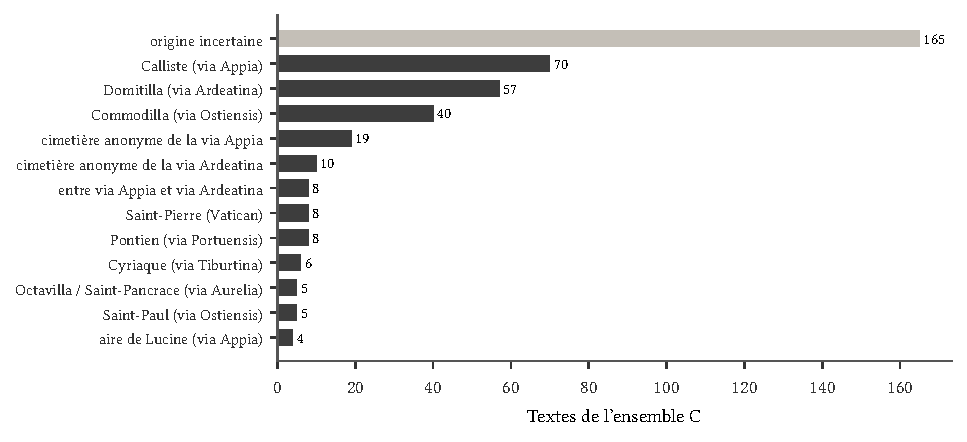
\includegraphics[width=0.88\linewidth]{figures/fig_cimetieres.pdf}
\caption{Rattachement topographique des textes funéraires selon l’EDB (secteurs d’au moins quatre textes).}\label{fig:cimetieres}
\end{figure}

La répartition par période des trois grands ensembles diffère. Les textes de Commodilla se concentrent dans les dernières décennies (1, 7, 13 et 19 textes pour les quatre périodes), alors que ceux de Calliste (7, 23, 19, 21) et de Domitilla (7, 14, 12, 24) sont mieux répartis. Ces chiffres sont trop faibles pour fonder une chronologie de l’occupation des cimetières : ils dépendent de ce qui a été conservé, fouillé et publié, et de la proportion de textes datés dans chaque secteur. Ils indiquent seulement que la composition topographique du corpus change avec le temps, ce qui doit être pris en compte avant toute comparaison chronologique du formulaire.

\section{Les lieux de conservation}

L’EDB indique un lieu de conservation pour \st{nConsConnue} textes funéraires (tableau~\ref{tab:conservation}). Les musées du Vatican (Lapidario Cristiano et Galleria Lapidaria) en réunissent la plus grande part ; viennent ensuite les catacombes elles-mêmes (Calliste, Domitilla et la basilique des Saints-Nérée-et-Achillée, Commodilla), le Museo Nazionale Romano, les Musées du Capitole et le Collegio Teutonico. Quelques pierres ont quitté Rome : un fragment du doublon 329/336 est conservé au lapidaire d’Ostie, et le \nnum{369} serait, selon l’EDB, conservé à Valence (Espagne). Ces indications n’ont pas été contrôlées sur place. Elles fournissent le point de départ de toute autopsie future.

% généré par scripts/04_generated.py
\begin{table}[tbp]\centering\small\caption{Lieu de conservation actuel indiqué par l’EDB (ensemble C ; 296 textes). Indication de la base, non contrôlée.}\label{tab:conservation}
\begin{tabular}{@{}l r@{}}\toprule Lieu de conservation & Textes\\\midrule
Musées du Vatican & 81 \\
catacombe de Calliste & 36 \\
basilique des Saints-Nérée-et-Achillée (Domitilla) & 24 \\
autres lieux (Coem. anonymum ad viam Appiam) & 19 \\
Museo Nazionale Romano & 16 \\
autres lieux (Coem. Domitillae pars inferior) & 13 \\
Musées du Capitole & 12 \\
autres lieux (Coem. anonymum ad viam Ardeatinam) & 9 \\
autres lieux (coem. Domitillae, aula supra coemeterium) & 7 \\
Collegio Teutonico & 7 \\
catacombe de Commodilla & 5 \\
autres lieux (Antiquarium del Celio) & 5 \\
autres lieux (s. Cecilia in Trastevere) & 4 \\
autres lieux (Fossombrone (PU)   ; Lapidario Diocesano) & 4 \\
autres lieux (s. Paolo f.l.m.) & 4 \\
autres lieux (Basilica s.Pauli apostoli) & 4 \\
autres lieux & 46 \\
\bottomrule\end{tabular}\end{table}


\section{Ce que ces données permettent et ne permettent pas de dire}

Le rattachement topographique de l’EDB est une information éditoriale. Il peut reposer sur un lieu de découverte documenté, sur une tradition de collection ou sur un raisonnement des éditeurs ; il ne donne ni la position de la tombe dans le cimetière, ni son contexte stratigraphique, ni sa relation avec un sanctuaire de martyr. La série d’origine incertaine réunit plusieurs des textes les plus importants du corpus (\nnums{73}, 232 et 447), dont le contexte funéraire est inconnu. D’autres textes décisifs reçoivent en revanche de l’EDB un rattachement précis : l’épitaphe de Quintilianus, qui mentionne la Trinité (\nnum{474}), et celle de Privata (\nnum{38}) proviennent du cimetière à ciel ouvert proche de la basilique Saint-Pierre ; le texte qui mentionne l’Esprit saint (\nnum{249}) est rattaché au cimetière de Nicomède, sur la via Nomentana.

Une donnée nouvelle mérite d’être relevée pour la discussion de la sépulture \emph{ad sanctos}. Le \nnum{232}, qui célèbre l’obtention d’une sépulture « au seuil des saints », est d’origine incertaine ; le \nnum{387}, dont la mention d’un emplacement acheté \emph{[ad limina Petri et] Pauli sub episcopatu Si[rici]} est en grande partie restituée, n’est pas apparié à l’EDB. Aucun des deux textes ne peut donc être localisé dans une basilique déterminée sur la seule foi des bases.

L’étude topographique du corpus suppose un retour aux éditions, notice par notice : identification du cimetière et de la région, mention du lieu de découverte et du lieu de conservation, support et dimensions. Les données de l’EDB intégrées aux notices permettent désormais d’organiser ce retour.

\section{La notice 439 et la provenance romaine}

L’attribution romaine d’une notice reste douteuse. Le \nnum{439}, épitaphe de Petulus datée par le consulat de Stilichon, est identifié comme CIL XIV 3896 = \emph{Inscriptiones Italiae} IV 1, 543. Le volume XIV du CIL couvre le Latium ancien ; dans l’export EDCS de 2022, les numéros CIL XIV 3850–3950 relèvent pour la plupart de Tibur et de ses environs (49 fiches sur 94), et seule la fiche correspondant au \nnum{439} est classée « Roma ». L’EDB la range dans la série d’origine incertaine. La notice est exclue des analyses topographiques propres à Rome.

\chapter{Supports, exécution et signes}\label{ch:supports}

Les notices issues de l’EDCS ne contenaient aucune donnée matérielle : ni support, ni matériau, ni dimensions, ni signes figurés. Les fiches EpiDoc de l’EDB en fournissent pour \st{edbXmlC} des \st{nC} textes funéraires. Ces descriptions sont celles des rédacteurs de la base, nommés dans chaque notice ; elles reposent sur l’édition, sur les photographies et, pour une partie des pierres, sur l’autopsie de l’équipe de Bari. Elles n’ont pas été contrôlées ici et doivent être lues comme des données transmises.

\section{Supports, matériaux et techniques}

% généré par scripts/04_generated.py
\begin{table}[tbp]\centering\small\caption{Support, matériau et technique d’exécution selon les fiches EpiDoc de l’EDB (ensemble C ; 429 fiches).}\label{tab:supports}
\begin{tabular}[t]{@{}l r@{}}\toprule Support & N\\\midrule plaque & 349\\ non précisé & 53\\ sarcophage & 12\\ enduit de mortier & 11\\ paroi & 3\\ brique & 1\\\bottomrule\end{tabular}\hspace{1.2em}\begin{tabular}[t]{@{}l r@{}}\toprule Matériau & N\\\midrule marbre & 361\\ non précisé & 53\\ mortier & 11\\ enduit & 3\\ maçonnerie de briques & 1\\\bottomrule\end{tabular}\hspace{1.2em}\begin{tabular}[t]{@{}l r@{}}\toprule Exécution & N\\\midrule gravée & 360\\ non précisé & 54\\ tracée dans le mortier frais & 11\\ peinte & 3\\ graffitée & 1\\\bottomrule\end{tabular}\end{table}


La plaque de marbre domine très largement (tableau~\ref{tab:supports}). C’est le support ordinaire de la fermeture d’un \emph{loculus} ou d’une tombe à formes dans les catacombes et dans les cimetières à ciel ouvert. Pour \st{nPlaquesMes} plaques dont les deux dimensions sont données, la hauteur médiane est de \st{medH}~cm et la largeur médiane de \st{medW}~cm ; les largeurs s’étendent de \st{minW} à \st{maxW}~cm. Ces mesures ne disent rien de l’état complet du monument : une partie des plaques est fragmentaire.

Trois autres groupes, plus petits, méritent l’attention.

\emph{Les sarcophages} (\st{nSarco} textes : \nnums{\st{sarcolist}}). Le texte est alors gravé sur la cuve ou le couvercle d’un monument coûteux. Plusieurs de ces textes figurent parmi les plus longs et les plus élaborés du corpus : le poème de Maximilla et la notice de Lucceia (\nnum{306}, 72 × 212 cm, Platonia de Saint-Sébastien), l’épitaphe métrique de Felicitas (\nnum{470}), l’épitaphe de Cassia, \emph{clarissima femina} (\nnum{15}).

\emph{Les inscriptions tracées dans le mortier frais} (\st{nMortier} textes : \nnums{\st{mortierlist}}). Le texte est incisé au moment de la fermeture de la tombe, dans l’enduit qui scelle le \emph{loculus}. Ces inscriptions sont souvent brèves ; l’une d’elles (\nnum{311}) porte la formule \emph{in Chr(isto)} et un chrisme.

\emph{Les inscriptions peintes et graffitées} (\nnums{\st{peinteslist}} pour la peinture, 325 pour le graffite sur brique). L’inscription peinte du \nnum{206} est celle pour laquelle l’EDB donne une date (377) incompatible avec la formule consulaire (370) : la date de la base est vraisemblablement fautive.

L’EDB qualifie de métriques dix textes (\nnums{\st{metrlist}}). Cette qualification est incomplète : d’autres textes du corpus sont métriques ou rythmés (par exemple le \nnum{306}, que l’EDB ne qualifie pas ainsi, ou le \nnum{352}, recueilli dans les \emph{Carmina Latina Epigraphica}). Elle ne peut servir à mesurer la part des épitaphes en vers.

\section{Reproductions disponibles}

L’EDB signale une reproduction pour \st{nFacsim} textes funéraires : photographies de la Pontificia Commissione di Archeologia Sacra, dessins de l’ICVR I de De Rossi, reproductions tirées de publications (Perret 1851, ICVR IV, corpus régionaux). Ces images sont protégées (« Rights Reserved — Free Access via Epigraphic Database Bari ») ; elles n’ont pas été reproduites. Leur existence est signalée dans chaque notice, car elle définit le programme d’un contrôle photographique.

\section{Les signes chrétiens}

\subsection{Un marquage invisible dans la première base}

L’EDB décrit des chrismes et des croix sur \st{nSignesA} textes du catalogue, dont \st{nSignesC} textes funéraires, soit \st{pSignesC}~\% des \st{edbAppC} textes funéraires appariés. L’EDCS n’en signale aucun, sauf au \nnum{38}, où le monogramme est rendu par un mot développé. Ce chiffre est un minimum : les textes tronqués des listes de résultats peuvent omettre un signe placé en fin de texte, et les fiches EpiDoc de 2019 ne décrivent pas toujours le décor. Il dépend aussi de la description de l’EDB, qui n’a pas été vérifiée sur photographie.

\begin{table}[tbp]\centering\small
\caption{Types de signes décrits par l’EDB (ensemble C ; un texte peut porter plusieurs signes).}\label{tab:typessignes}
\begin{tabular}{@{}l r@{}}\toprule Signe & Textes\\\midrule
chrisme & 49\\ chrisme avec alpha et oméga & 23\\ croix monogrammatique & 10\\ croix monogrammatique avec alpha et oméga & 5\\ croix & 2\\ chrisme radié, alpha et oméga seuls, croix gammée & 1 chacun\\\bottomrule
\end{tabular}
\end{table}

Le chrisme, simple ou accompagné de l’alpha et de l’oméga, domine (tableau~\ref{tab:typessignes}). La croix monogrammatique, où la haste du P se combine avec une croix, apparaît plus rarement. L’EDB décrit en outre des signes qui ne sont pas comptés ici comme christiques : oiseaux, palmes, feuilles, couronnes, orants.

\subsection{Une part qui décroît}

Rapportée aux textes appariés de chaque période, la part des textes portant un chrisme ou une croix décroît : environ un texte sur quatre dans les années 340–359, un sur dix dans les années 390–403 (tableau~\ref{tab:signesper}, figure~\ref{fig:signes}). Cette tendance doit être interprétée avec prudence. Elle peut traduire un changement des pratiques de gravure ; elle peut aussi tenir à la composition topographique du corpus, qui change avec le temps (chapitre~\ref{ch:provenance}), ou à l’inégale description du décor selon les secteurs et les rédacteurs de la base. Elle n’autorise aucune conclusion sur l’intensité de l’identité chrétienne.

% généré par scripts/04_generated.py
\begin{table}[tbp]\centering\small\caption{Textes de l’ensemble C portant un chrisme ou une croix selon l’EDB, par période, rapportés aux textes appariés à une fiche EDB.}\label{tab:signesper}
\begin{tabular}{@{}l r r r@{}}\toprule Période & Signes & Textes appariés & \%\\\midrule
340–359 & 12 & 50 & 24,0 \\
360–374 & 24 & 114 & 21,1 \\
375–389 & 16 & 132 & 12,1 \\
390–403 & 15 & 147 & 10,2 \\
\bottomrule\end{tabular}\end{table}


\begin{figure}[tbp]\centering
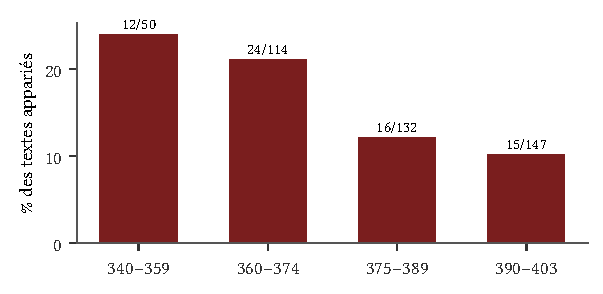
\includegraphics[width=0.62\linewidth]{figures/fig_signes.pdf}
\caption{Part des textes funéraires appariés portant un chrisme ou une croix selon l’EDB, par période.}\label{fig:signes}
\end{figure}

\subsection{Signes et formulaire}

Les textes qui portent un signe sont plus souvent pourvus de la formule \emph{in pace} que les autres : \st{ipSigne} contre \st{ipSansSigne}. L’association est nette, mais elle ne démontre pas une relation de sens. Les textes à signe décrit sont aussi, en moyenne, mieux conservés et mieux documentés ; et le signe, comme la formule, appartient à un même registre de marquage chrétien du monument. La mesure montre seulement que signe et formule ne se substituent pas l’un à l’autre : ils se cumulent.

\subsection{Quand le signe tient lieu de mot}

Dans quatre textes, la question du signe touche directement le vocabulaire. Au \nnum{38}, l’EDB transcrit \emph{in pace ((monogramma Christi))} là où l’EDCS donne \emph{in pace Chr(isti)}, et l’estampage universitaire montre un christogramme après IN PACE. Aux \nnums{140} et 151 (\emph{in pace Chr(isti)}) et au \nnum{311} (\emph{in Chr(isto)}), les deux bases transcrivent un mot abrégé, mais l’EDB décrit un chrisme sur le support. Il est probable que, dans ces trois textes, l’abréviation développée rende un monogramme employé comme compendium du nom du Christ ; il n’est pas exclu qu’elle coexiste avec un chrisme décoratif distinct. Les deux bases, et sans doute les éditeurs qu’elles suivent, ont fait des choix de transcription différents pour des situations peut-être identiques. La conséquence est traitée au chapitre~\ref{ch:dieu_christ} : ces quatre textes ne peuvent être comptés comme des mentions écrites du Christ sans contrôle des photographies.

% généré par scripts/04_generated.py
\begin{longtable}{@{}r r p{0.7\linewidth}@{}}\caption{Signes chrétiens décrits par l’EDB (fiches EpiDoc de 2019 et texte des listes de résultats de 2026), ensemble A.}\label{tab:signes}\\\toprule N° & Année & Signes\\\midrule\endfirsthead\toprule N° & Année & Signes\\\midrule\endhead\bottomrule\endfoot
4 & 341 & chrisme \\
9 & 343 & chrisme \\
16 & 346 & chrisme \\
22 & 348 & chrisme et chrisme radié \\
24 & 348 & croix \\
34 & 350 & chrisme \\
38 & 352 & chrisme \\
43 & 355 & chrisme et chrisme avec alpha et oméga \\
46 & 356 & chrisme \\
49 & 358 & chrisme \\
50 & 358 & chrisme \\
55 & 359 & chrisme et chrisme avec alpha et oméga \\
60 & 361 & chrisme \\
61 & 361 & chrisme \\
68 & 362 & chrisme et chrisme avec alpha et oméga \\
73 & 363 & alpha et oméga, chrisme, croix et croix gammée \\
94 & 365 & chrisme \\
95 & 365 & croix monogrammatique avec alpha et oméga \\
99 & 366 & chrisme \\
100 & 366 & chrisme \\
106 & 367 & chrisme \\
109 & 367 & chrisme et chrisme avec alpha et oméga \\
118 & 367 & chrisme \\
120 & 367 & chrisme \\
124 & 367 & chrisme \\
128 & 368 & chrisme \\
136 & 370 & chrisme et chrisme avec alpha et oméga \\
139 & 370 & chrisme \\
140 & 370 & chrisme \\
142 & 370 & chrisme \\
143 & 371 & chrisme et chrisme avec alpha et oméga \\
146 & 371 & chrisme et chrisme avec alpha et oméga \\
147 & 371 & chrisme \\
151 & 371 & chrisme \\
160 & 372 & chrisme avec alpha et oméga \\
168 & 373 & croix monogrammatique \\
175 & 374 & chrisme avec alpha et oméga \\
179 & 375 & chrisme et chrisme avec alpha et oméga \\
183 & 375 & chrisme \\
185 & 375 & chrisme avec alpha et oméga \\
186 & 375 & chrisme \\
191 & 376 & chrisme \\
193 & 376 & chrisme et chrisme avec alpha et oméga \\
209 & 378 & chrisme et chrisme avec alpha et oméga \\
213 & 380 & chrisme et croix monogrammatique \\
225 & 381 & chrisme avec alpha et oméga \\
247 & 383 & chrisme \\
260 & 384 & chrisme et chrisme avec alpha et oméga \\
273 & 384 & chrisme et chrisme avec alpha et oméga \\
275 & 385 & chrisme et chrisme avec alpha et oméga \\
276 & 385 & chrisme \\
300 & 388 & croix monogrammatique avec alpha et oméga \\
304 & 389 & chrisme et chrisme avec alpha et oméga \\
311 & 388 & chrisme \\
321 & 390 & chrisme \\
324 & 390 & chrisme avec alpha et oméga \\
344 & 392 & croix monogrammatique et croix monogrammatique avec alpha et oméga \\
348 & 392 & croix monogrammatique \\
349 & 392 & chrisme avec alpha et oméga \\
357 & 393 & croix monogrammatique \\
369 & 395 & croix monogrammatique \\
376 & 395 & chrisme, chrisme avec alpha et oméga, croix monogrammatique et croix monogrammatique avec alpha et oméga \\
400 & 397 & chrisme et croix monogrammatique \\
402 & 397 & croix monogrammatique \\
430 & 399 & croix monogrammatique \\
431 & 399 & chrisme et chrisme avec alpha et oméga \\
434 & 397 & chrisme et chrisme avec alpha et oméga \\
453 & 401 & chrisme avec alpha et oméga \\
454 & 401 & croix monogrammatique avec alpha et oméga \\
465 & 402 & chrisme \\
\end{longtable}



\part{Langue et formulaire}
\chapter{Le formulaire funéraire}\label{ch:formulaire}

\section{Une règle de relevé unique}

Le relevé du formulaire distingue trois situations que la notation épigraphique sépare et que les comptages confondent souvent : une expression gravée en toutes lettres ; une expression abrégée sur la pierre, dont le développement est éditorial ; une expression dont tout ou partie des lettres est restitué dans une lacune. Dans \emph{in p(ace)}, l’abréviation est gravée et seul le développement appartient à l’éditeur ; dans \emph{in [pace]}, les lettres du second mot sont absentes du support. Une quatrième situation, plus rare, est celle de la correction éditoriale : \emph{i⸢n⸣ pace} signale une lettre gravée différente de la lettre attendue (M pour N aux \nnums{121} et 150), non une lacune.

Chaque élément du formulaire est recherché par une expression régulière appliquée au texte normalisé (\emph{u/v} et \emph{i/j} unifiés), et chaque occurrence reçoit le statut de ses lettres. Une expression interrompue par une fin de ligne (\emph{pa/ce}) est reconnue comme une seule occurrence. Un texte est compté « sans restitution » lorsqu’au moins une occurrence de l’élément ne comporte aucune lettre restituée ; il est compté « avec restitution » lorsqu’au moins une occurrence, restituée ou non, est présente. Les règles exactes, les formes relevées et les notices concernées sont publiées au chapitre~\ref{ch:rep_formulaire}.

\section{La formule \emph{in pace}}

Dans l’ensemble C, \emph{in pace} est attestée dans \st{ip_tot} textes (\st{ip_pct}~\%), répartis en quatre groupes exclusifs (figure~\ref{fig:inpace}) :

\begin{itemize}
\item \st{ip_ecrit} textes la donnent en toutes lettres, sans lettre corrigée (\st{ip_ecrit_pct}~\% de l’ensemble) ;
\item \st{ip_abrege} textes la donnent abrégée (\emph{in p(ace)}), sans restitution ni correction ;
\item \st{ip_corrige} textes la donnent avec une correction éditoriale, sans restitution (\nnums{76}, 121, 150 et 359) ;
\item \st{ip_restitue} textes ne l’attestent que par une restitution.
\end{itemize}

\begin{figure}[tbp]\centering
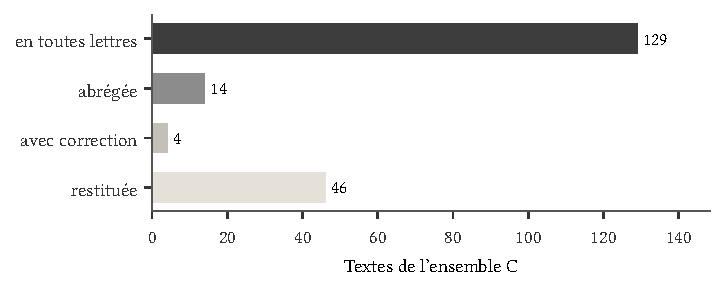
\includegraphics[width=0.7\linewidth]{figures/fig_inpace.pdf}
\caption{La formule \emph{in pace} dans l’ensemble C : quatre catégories exclusives (n = \st{ip_tot}).}\label{fig:inpace}
\end{figure}

Près d’un quart des attestations repose donc sur une restitution. Ces restitutions ne sont pas arbitraires : la formule est si fréquente que les éditeurs la restituent lorsque \emph{in} ou \emph{pace} subsiste, ou lorsque l’espace et la structure du texte la suggèrent. Mais elles reproduisent, par construction, la fréquence que l’on cherche à mesurer. L’attestation sans restitution (\st{ip_sansrest} textes, 31,6~\%) est la seule base indépendante.

Sur l’ensemble initial de 468 textes (C\textsubscript{0}), le même relevé donne \st{ipz_tot} attestations : \st{ipz_ecrit} en toutes lettres, \st{ipz_abrege} abrégées, \st{ipz_corrige} corrigées et \st{ipz_restitue} restituées. La version précédente du manuscrit comptait 132 attestations en toutes lettres et 46 restituées. L’écart tient à la notice 341, dont le texte commence par \emph{in p]ace} : la lacune initiale emporte le P, et l’attestation doit être classée parmi les restitutions. Le passage de C\textsubscript{0} à C (fusion des doublons, exclusion du \nnum{98}, jonction du \nnum{394}, inclusion du \nnum{406}) retire en outre deux attestations en toutes lettres et une restituée. Les listes complètes sont données ci-dessous.

% généré par scripts/04_generated.py
\begin{description}[style=nextline,leftmargin=1.5em,font=\normalfont\scshape]
\item[En toutes lettres, sans correction] (129 textes) 4, 9, 10, 16, 20, 22, 26, 28, 33, 34, 35, 38, 42, 45, 46, 47, 49, 55, 56, 57, 59, 61, 63, 68, 70, 72, 75, 78, 80, 94, 99, 102, 104, 115, 117, 119, 120, 125, 126, 127, 128, 130, 132, 133, 139, 140, 143, 144, 145, 151, 155, 156, 157, 166, 168, 172, 179, 183, 184, 185, 191, 196, 200, 202, 205, 207, 210, 211, 221, 223, 231, 233, 234, 237, 240, 241, 250, 260, 261, 271, 276, 284, 287, 288, 291, 295, 298, 300, 303, 304, 320, 323, 336, 346, 347, 351, 353, 361, 365, 367, 368, 369, 371, 374, 376, 381, 383, 388, 389, 396, 399, 402, 403, 404, 409, 411, 416, 419, 421, 427, 431, 444, 446, 448, 451, 453, 460, 463, 469.
\item[Abrégée, sans restitution ni correction] (14 textes) 17, 41, 54, 66, 81, 83, 124, 134, 203, 213, 279, 296, 420, 470.
\item[Avec correction éditoriale, sans restitution] (4 textes) 76, 121, 150, 359.
\item[Seulement avec restitution] (46 textes) 3, 6, 40, 53, 69, 73, 74, 77, 90, 93, 158, 162, 182, 186, 187, 190, 198, 226, 246, 258, 268, 272, 283, 302, 305, 322, 325, 337, 341, 343, 344, 350, 355, 362, 364, 370, 401, 408, 410, 428, 429, 430, 445, 450, 464, 471.
\end{description}


\section{Fréquences des éléments du formulaire}

Le tableau~\ref{tab:formulaire} donne, pour vingt et un éléments, le nombre de textes de l’ensemble C où l’élément est attesté, avec et sans restitution. L’écart entre les deux colonnes mesure la dépendance de chaque élément à l’égard des restitutions. Il est particulièrement élevé pour \emph{bene merenti} (86 contre 53), pour \emph{coniux} et ses équivalents (71 contre 45) et pour \emph{depositio} (247 contre 179) : ces mots occupent souvent des positions que les éditeurs restituent d’après la structure attendue du texte.

% généré par scripts/04_generated.py
\begin{table}[tbp]\centering\small
\caption{Éléments du formulaire dans l’ensemble C (n = 465) : textes où l’élément est attesté, restitutions comprises, et textes où il l’est au moins une fois sans restitution (abréviations et corrections admises).}\label{tab:formulaire}
\begin{tabular}{@{}l r r r r@{}}\toprule Élément & Avec rest. & \% & Sans rest. & \% \\\midrule
\lat{in pace} & 193 & 41,5 & 147 & 31,6 \\
\lat{depositio / depositus} & 247 & 53,1 & 179 & 38,5 \\
\lat{vixit (et variantes)} & 264 & 56,8 & 189 & 40,6 \\
\lat{bene merenti} & 86 & 18,5 & 53 & 11,4 \\
\lat{fecit / fecerunt} & 74 & 15,9 & 61 & 13,1 \\
\lat{hic (iacet, positus, requiescit…)} & 33 & 7,1 & 27 & 5,8 \\
\lat{requiescit / quiescit} & 37 & 8,0 & 29 & 6,2 \\
\lat{decessit / recessit / defunctus} & 36 & 7,7 & 28 & 6,0 \\
\lat{dormitio / dormit} & 6 & 1,3 & 3 & 0,6 \\
\lat{locus} & 26 & 5,6 & 19 & 4,1 \\
\lat{bisomus / trisomus / quadrisomus} & 10 & 2,2 & 6 & 1,3 \\
\lat{achat (emere, comparare)} & 7 & 1,5 & 4 & 0,9 \\
\lat{fossor} & 1 & 0,2 & 1 & 0,2 \\
\lat{coniux / compar / maritus / uxor} & 71 & 15,3 & 45 & 9,7 \\
\lat{virginius / virginia} & 5 & 1,1 & 3 & 0,6 \\
\lat{filius / filia} & 33 & 7,1 & 27 & 5,8 \\
\lat{parentes / pater / mater} & 29 & 6,2 & 24 & 5,2 \\
\lat{dulcissimus / carissimus} & 30 & 6,5 & 24 & 5,2 \\
\lat{plus minus} & 50 & 10,8 & 42 & 9,0 \\
\lat{se vivo / se viva} & 18 & 3,9 & 10 & 2,2 \\
\lat{post consulatum} & 23 & 4,9 & 15 & 3,2 \\
\bottomrule\end{tabular}\end{table}


Trois éléments forment le noyau du formulaire : la durée de vie (\emph{vixit}), la date de la déposition (\emph{depositus}, \emph{depositio}) et la formule \emph{in pace}. Les autres éléments sont minoritaires. La commémoration par un parent ou un conjoint (\emph{fecit}, \emph{bene merenti}), l’expression du repos (\emph{requiescit}, \emph{hic iacet}) et la mention du lieu (\emph{locus}, \emph{bisomus}) n’atteignent chacune qu’une fraction des textes.

\section{Variations chronologiques}

La figure~\ref{fig:formulaire} donne la part des textes de chaque période qui attestent l’élément sans restitution. Trois observations peuvent être formulées, avec des réserves différentes.

\begin{figure}[tbp]\centering
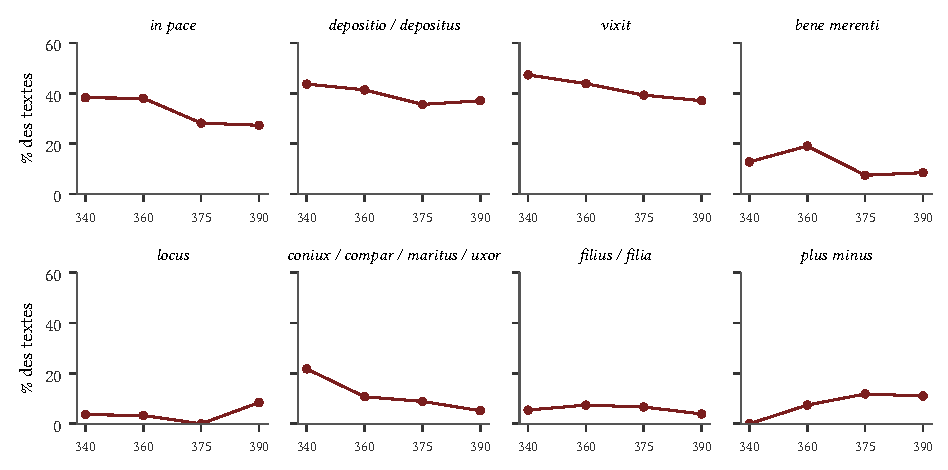
\includegraphics[width=\linewidth]{figures/fig_formulaire.pdf}
\caption{Part des textes de chaque période attestant l’élément sans restitution (ensemble C ; périodes 340–359, 360–374, 375–389, 390–403 ; effectifs \st{perC0}, \st{perC1}, \st{perC2}, \st{perC3}).}\label{fig:formulaire}
\end{figure}

\emph{Recul apparent des formules les plus fréquentes.} La part des textes portant \emph{in pace} sans restitution passe de 38~\% (21/55 ; intervalle de Wilson à 95~\% : 26,5–51,4) et 38~\% (46/121) dans les deux premières périodes à 28~\% (38/135) et 27~\% (42/154 ; 20,9–34,8) dans les deux dernières. \emph{Vixit} et \emph{depositio} reculent dans des proportions comparables. Or la part restituée des textes augmente dans le même temps : le ratio moyen de lettres restituées passe de 0,26 (340–359) à 0,29 (390–403). Avec les restitutions, la part d’\emph{in pace} est de 45~\%, 45~\%, 38~\% et 41~\% : les intervalles se recouvrent largement. Le recul apparent peut donc tenir, au moins en partie, à l’état de conservation des textes tardifs. Il ne peut être interprété comme un changement de pratique.

\emph{Recul des termes de la relation conjugale.} Les mots \emph{coniux}, \emph{compar}, \emph{maritus} et \emph{uxor} sont attestés sans restitution dans 12 textes sur 55 en 340–359 (21,8~\% ; 12,9–34,4) et dans 8 sur 154 en 390–403 (5,2~\% ; 2,7–9,9). Les intervalles ne se recouvrent pas. L’écart est plus net que pour les autres éléments, mais il repose sur de petits effectifs, et la composition topographique du corpus change entre les deux périodes (chapitre~\ref{ch:provenance}).

\emph{Apparition de nouveaux éléments dans les dernières décennies.} \emph{Plus minus} est absent des textes de 340–359 et figure dans 17 textes de 390–403 sans restitution (11,0~\%). Les mentions de l’emplacement (\emph{locus} : 13 textes en 390–403 contre 2 en 340–359), de l’achat (4 textes, tous de 390–403) et de la préparation du vivant (\emph{se vivo} : aucun texte avant 375) apparaissent ou progressent. L’expression \emph{hic iacet} et ses variantes suivent la même pente (1 texte en 340–359, 13 en 390–403). Ces observations convergent avec la chronologie admise du formulaire romain, où les mentions d’achat et d’emplacement se développent à la fin du \textsc{iv}\textsuperscript{e} siècle ; elles ne la démontrent pas à elles seules, car les effectifs restent faibles et les textes d’achat sont concentrés dans quelques secteurs.

\section{Ce que mesure le formulaire}

Le formulaire décrit des choix de rédaction et de gravure. Il ne mesure directement ni la foi des défunts, ni celle des commanditaires. La présence d’\emph{in pace} sur quatre textes sur dix est un fait de pratique épigraphique : elle associe le défunt à un vocabulaire du repos d’usage chrétien, sans préciser la nature de ce repos. Son absence ne signifie pas l’absence de conviction chrétienne : de nombreux textes très brefs ne comportent que le nom, l’âge et la date, et une partie d’entre eux porte un chrisme (chapitre~\ref{ch:supports}). Les chapitres consacrés au vocabulaire religieux (chapitres~\ref{ch:typologie} à \ref{ch:rep_religieux}) reprennent la question sur les textes qui vont au-delà du formulaire.

\chapter{La langue des épitaphes}\label{ch:langue}

Les épitaphes datées offrent un échantillon daté du latin écrit à Rome dans la seconde moitié du \textsc{iv}\textsuperscript{e} siècle. Elles ne donnent pas pour autant un accès direct à la langue parlée. Le texte gravé passe par un rédacteur, un modèle de formulaire et un lapicide ; le texte édité passe ensuite par les normalisations de l’éditeur et de la base. Ce chapitre décrit ce que le texte transmis permet d’observer, en séparant les faits de graphie, les abréviations et les choix morphologiques qui relèvent du développement éditorial.

\section{Graphies : ce que signalent les corrections éditoriales}

Le texte de l’EDCS est normalisé : la lettre attendue figure dans le texte, la lettre déclarée gravée est conservée dans la notation \emph{<attendu=gravé>}, rendue ici par les demi-crochets ⸢ ⸣ et l’apparat de chaque notice. L’état 2022 de la base signale ainsi \st{nCorrOcc} corrections dans \st{nCorrNotices} notices de l’ensemble A. Ces données ne constituent pas une transcription diplomatique : elles reflètent ce que les éditeurs ont jugé utile de signaler, et une graphie non standard qu’un éditeur aurait conservée sans la corriger n’y figure pas.

Leur typologie est néanmoins nette (tableau~\ref{tab:graphies}). Quatre phénomènes dominent :

\begin{itemize}
\item \emph{le bêtacisme}, échange de B et de V (81 occurrences) : \emph{B} pour \emph{v} dans 72 cas (\emph{⸢b⸣ixit}, \emph{iu⸢b⸣enis}), \emph{V} pour \emph{b} dans 9 ;
\item \emph{la confusion de E et de I} (60 occurrences), dans les deux sens (\emph{mens⸢e⸣s} gravé MENSIS, \emph{⸢i⸣n} gravé EN) ;
\item \emph{la confusion de O et de U} (46 occurrences), notamment dans la désinence d’\emph{annos}, gravée ANNVS (28 occurrences dans 26 notices), et dans les formes \emph{Theudosius} et \emph{Neuterius} des noms consulaires ;
\item \emph{les graphies du Y} (18 occurrences), rendu par I ou par V dans les noms d’origine grecque (\emph{Eut⸢y⸣chius}).
\end{itemize}

Viennent ensuite C pour G (13), N pour M devant labiale ou en finale (12), S pour X (6) et E pour A (5). Ces phénomènes sont ceux que décrivent les grammaires du latin tardif ; ils ne sont pas propres aux inscriptions chrétiennes.\footnote{V.~Väänänen, \emph{Introduction au latin vulgaire}, 3\textsuperscript{e} éd., Paris, 1981 ; J.~N.~Adams, \emph{Social Variation and the Latin Language}, Cambridge, 2013. Notices bibliographiques vérifiées ; aucun renvoi de page n’est donné, faute de consultation des passages.} Une partie des corrections relève par ailleurs de la lecture plutôt que de la langue : les dix-huit cas où un I est lu à la place d’un T attendu peuvent tenir à une barre horizontale effacée ou mal gravée, ce qu’une photographie seule permettrait de décider.

% généré par scripts/04_generated.py
\begin{longtable}{@{}l l r l p{0.45\linewidth}@{}}
\caption{Corrections éditoriales signalées par l’EDCS (état 2022, ensemble A) : lettre attendue, lettre déclarée gravée, occurrences, phénomène, notices. Correspondances attestées au moins deux fois.}\label{tab:graphies}\\
\toprule Attendu & Gravé & Occ. & Phénomène & Notices\\\midrule\endfirsthead\toprule Attendu & Gravé & Occ. & Phénomène & Notices\\\midrule\endhead\bottomrule\endfoot
\lat{v} & B & 72 & bêtacisme & {\footnotesize 4, 6, 22, 24, 26, 34, 40, 47, 56, 63, 72, 83, 89, 90, 91, 106, 112, 113, 118, 119, 120, 124, 144, 172, 184, 194, 207, 208, 215, 217, 234, 235, 261, 272, 281, 301, 313, 332, 347, 352, 365, 366, 374, 402, 407, 408, 417, 440, 441, 444, 468, 475} \\
\lat{o} & V & 44 & confusion o/u & {\footnotesize 32, 54, 55, 69, 94, 104, 130, 161, 191, 193, 209, 225, 275, 281, 288, 289, 299, 320, 322, 323, 327, 336, 346, 347, 353, 359, 365, 374, 375, 376, 379, 400, 419, 421, 427, 431, 443, 466, 470, 473, 475, 478} \\
\lat{e} & I & 43 & confusion e/i & {\footnotesize 4, 25, 28, 34, 55, 60, 80, 84, 94, 124, 151, 157, 191, 193, 260, 261, 287, 306, 337, 347, 353, 359, 365, 366, 367, 381, 389, 390, 395, 411, 423, 431, 441, 443, 446} \\
\lat{t} & I & 18 & i pour t (lecture) & {\footnotesize 37, 63, 132, 136, 153, 164, 186, 231, 245, 296, 306, 308, 333, 371, 433} \\
\lat{i} & E & 17 & confusion e/i & {\footnotesize 27, 40, 50, 54, 70, 76, 100, 111, 125, 306, 353, 364, 368, 388, 391, 443} \\
\lat{y} & I & 13 & graphie de y & {\footnotesize 1, 145, 172, 233, 238, 276, 308, 352, 391, 417, 418, 419, 424} \\
\lat{g} & C & 13 & c pour g & {\footnotesize 19, 35, 99, 201, 221, 231, 304, 306, 352, 353, 354, 359, 366} \\
\lat{m} & N & 12 & n pour m & {\footnotesize 23, 36, 46, 119, 126, 184, 217, 275, 365, 419, 424} \\
\lat{b} & V & 9 & bêtacisme & {\footnotesize 85, 123, 125, 276, 340, 357, 380, 382, 470} \\
\lat{V} & B & 7 &  & {\footnotesize 55, 90, 97, 128, 416} \\
\lat{x} & S & 6 & s pour x & {\footnotesize 13, 130, 132, 272, 302, 304} \\
\lat{l} & I & 6 &  & {\footnotesize 186, 266, 287, 333, 359} \\
\lat{a} & E & 5 & e pour a & {\footnotesize 28, 214, 279, 466} \\
\lat{y} & V & 5 & graphie de y & {\footnotesize 223, 239, 338, 339, 340} \\
\lat{q} & O & 4 &  & {\footnotesize 111, 231, 388, 418} \\
\lat{o} & VM & 4 &  & {\footnotesize 291, 402} \\
\lat{c} & Q & 3 & q pour c & {\footnotesize 1, 184, 287} \\
\lat{K} & C & 3 &  & {\footnotesize 9, 128, 279} \\
\lat{c} & QV & 3 &  & {\footnotesize 59, 404, 405} \\
\lat{t} & D & 3 &  & {\footnotesize 182, 319, 402} \\
\lat{a} & O & 3 &  & {\footnotesize 448, 449, 451} \\
\lat{i} & V & 2 &  & {\footnotesize 44, 157} \\
\lat{vi} & BE & 2 &  & {\footnotesize 66, 458} \\
\lat{n} & V & 2 &  & {\footnotesize 85, 309} \\
\lat{n} & M & 2 &  & {\footnotesize 121, 150} \\
\lat{XV} & VX & 2 &  & {\footnotesize 128, 198} \\
\lat{u} & O & 2 & confusion o/u & {\footnotesize 143, 299} \\
\lat{i} & O & 2 &  & {\footnotesize 156, 275} \\
\lat{e} & Y & 2 &  & {\footnotesize 198, 303} \\
\lat{o} & I & 2 &  & {\footnotesize 231, 402} \\
\lat{o} & U & 2 &  & {\footnotesize 260, 282} \\
\lat{r} & B & 2 &  & {\footnotesize 308, 371} \\
\lat{r} & I & 2 &  & {\footnotesize 446, 464} \\
\end{longtable}
\noindent{\small Correspondances attestées une seule fois (54) : d/T (7); Fl/IT (7); ae/I (26); v/R (34); c/I (37); ag/VA (40); st/TS (60); C/K (62); tt/DD (72); i/U (115); te/S (131); o/EM (133); d/P (135); V/Y (142); s/RO (156); q/C (184); ibus/ATV (193); ba/PR (201); us/OM (204); e/A (205); o/A (205); G/C (211); h/A (215); F/E (219); ch/T (223); v/I (231); y/U (232); r/D (269); d/O (287); i/B (287); it/TI (296); b/P (299); hr/RH (306); te/I (306); is/SI (309); L/I (318); e/C (319); c/E (319); um/ON (320); t/S (336); i/C (340); u/Y (349); x/CS (353); i/Y (368); ly/IV (371); ri/K (371); ae/IS (381); r/S (404); s/R (406); rum/S (416); S/E (441); i/A (470); e/F (473); Fl/TI (473).}


Le corpus ne permet pas, en général, de mesurer une évolution chronologique de ces graphies : les corrections sont dispersées, et leur signalement dépend de l’éditeur de chaque volume des ICUR autant que du texte gravé. Une correspondance fait exception par sa répartition. La graphie ANNVS pour \emph{annos} apparaît dans 2 notices sur 55 en 340–359, 4 sur 123 en 360–374, 4 sur 139 en 375–389, puis dans 16 notices sur 160 en 390–403 (ensemble A, hors \nnum{98}). La concentration dans la dernière période est nette ; elle peut traduire l’extension d’une graphie phonétique de la finale, mais elle pourrait aussi tenir à l’atelier ou au secteur d’origine des textes, que l’on ne connaît que pour une partie d’entre eux. Elle mérite un contrôle sur les photographies. L’index des graphies (chapitre~\ref{ch:index}) et le répertoire du chapitre~\ref{ch:rep_graphies} donnent pour chaque correspondance la liste des notices.

\section{Abréviations}

La datation consulaire fournit l’essentiel des abréviations (tableau~\ref{tab:abrev}) : \emph{conss(ulibus)}, \emph{cons(ulibus)}, \emph{vv(iris) cc(larissimis)}, \emph{dd(ominis) nn(ostris)}, \emph{Aug(usto)}, \emph{Fl(avio)}. Le redoublement de la dernière consonne pour marquer le pluriel (\emph{conss.}, \emph{Augg.}, \emph{vv. cc.}) est fréquent. Viennent ensuite les éléments de l’âge (\emph{ann(os)}, \emph{m(enses)}, \emph{d(ies)}) et de la date (\emph{Kal(endas)}, \emph{dep(ositus)}, \emph{d(e)p(ositus)}). Dans l’ensemble C, la formule consulaire n’est écrite \emph{consulibus} en toutes lettres que dans sept textes (\nnums{7}, 22, 155, 199, 215, 260 et 265) ; la forme abrégée est la norme.

% généré par scripts/04_generated.py
\begin{table}[tbp]\centering\small\caption{Les abréviations les plus fréquentes de l’ensemble A : forme abrégée (lettres gravées), exemple de développement éditorial, occurrences.}\label{tab:abrev}
\begin{tabular}{@{}l l r@{}}\toprule Abrégé & Exemple & Occ.\\\midrule d & \lat{d(ies)} & 133 \\
kal & \lat{Kal(endas)} & 124 \\
conss & \lat{conss(ulibus)} & 119 \\
m & \lat{m(enses)} & 100 \\
aug & \lat{Aug(usto)} & 98 \\
ann & \lat{ann(os)} & 88 \\
fl & \lat{Fl(avio)} & 86 \\
cons & \lat{cons(ulibus)} & 76 \\
n & \lat{n(ostro)} & 68 \\
v & \lat{v(iro)} & 61 \\
c & \lat{c(larissimo)} & 60 \\
p & \lat{p(lus)} & 60 \\
que & \lat{qu(a)e} & 56 \\
dep & \lat{dep(ositus)} & 47 \\
cc & \lat{cc(larissimis)} & 37 \\
vv & \lat{vv(iris)} & 35 \\
dd & \lat{dd(ominis)} & 28 \\
nn & \lat{nn(ostris)} & 23 \\
dp & \lat{d(e)p(osita)} & 23 \\
an & \lat{an(nos)} & 19 \\
q & \lat{q(uae)} & 19 \\
non & \lat{Non(as)} & 17 \\
oct & \lat{Oct(obres)} & 16 \\\bottomrule\end{tabular}\hspace{1.5em}\begin{tabular}{@{}l l r@{}}\toprule Abrégé & Exemple & Occ.\\\midrule coss & \lat{co(n)ss(ulibus)} & 15 \\
vix & \lat{vix(it)} & 15 \\
dec & \lat{Dec(embres)} & 14 \\
sept & \lat{Sept(embres)} & 12 \\
ian & \lat{Ian(uarias)} & 12 \\
id & \lat{Id(us)} & 12 \\
iul & \lat{Iul(ias)} & 12 \\
feb & \lat{Feb(ruarias)} & 12 \\
s & \lat{s(upra)} & 11 \\
augg & \lat{Augg(ustis)} & 10 \\
k & \lat{K(alendas)} & 10 \\
mai & \lat{Mai(as)} & 10 \\
f & \lat{f(emina)} & 9 \\
cos & \lat{co(n)s(ulibus)} & 9 \\
con & \lat{con(sulibus)} & 8 \\
teodosio & \lat{T(h)eodosio} & 8 \\
aur & \lat{Aur(elio)} & 7 \\
mart & \lat{Mart(ias)} & 7 \\
mens & \lat{mens(es)} & 7 \\
cl & \lat{Cl(audio)} & 7 \\
nov & \lat{Nov(embres)} & 7 \\
pos & \lat{pos(t)} & 6 \\\bottomrule\end{tabular}\end{table}


\section{Morphologie : ce qui appartient à l’éditeur}

Le développement des abréviations est un acte éditorial. Il engage parfois un choix morphologique que la pierre ne tranche pas. L’exemple le plus net est l’expression de la durée de vie. Le texte normalisé de l’ensemble C contient la forme \emph{annos} dans 220 textes ; mais elle n’est écrite en toutes lettres que dans 45 d’entre eux. Il faut y ajouter les textes où la pierre porte ANNVS, que l’éditeur corrige en \emph{ann⸢o⸣s} : la désinence est alors gravée, sous une forme non standard. Dans les autres, la pierre porte \emph{ann.}, \emph{an.} ou un sigle, et l’accusatif est une décision de l’éditeur. À l’inverse, l’ablatif \emph{annis}, attesté dans 40 textes, est écrit en toutes lettres dans 29. Il en va de même pour \emph{menses} (103 textes, dont 15 en toutes lettres) et \emph{dies} (90 textes, dont 31 en toutes lettres).

Sur les seules formes écrites, l’accusatif de durée (\emph{vixit annos}) et l’ablatif (\emph{vixit annis}) coexistent dans toutes les périodes : 8 contre 8 textes en 340–359, 9 contre 7 en 390–403. Les effectifs sont trop faibles pour décrire une tendance, mais ils suffisent à montrer qu’une étude de la syntaxe de la durée fondée sur le texte développé mesurerait d’abord les habitudes des éditeurs.

La même prudence s’applique aux formes de la déposition. Le texte normalisé donne \emph{depositus} dans 122 textes et \emph{deposita} dans 109, mais ces formes ne sont écrites en toutes lettres que dans 36 et 47 textes ; ailleurs, \emph{dep.} ou \emph{d. p.} est développé selon le sexe du défunt, lorsque celui-ci est connu par ailleurs, ou selon l’usage de l’éditeur. Le substantif \emph{depositio} n’est écrit en toutes lettres qu’une fois (\nnum{448}).

\section{Registre et composition}

La très grande majorité des textes relève d’un formulaire bref, où la langue se réduit à quelques syntagmes figés. Une dizaine de textes s’en écartent par la versification ou par une prose plus élaborée : les épitaphes métriques de Felicitas (\nnum{470}), d’Eutychius (\nnum{352}) ou de Maximilla (\nnum{306}), les textes du \nnum{232} et du \nnum{73}. Ils sont étudiés pour leur contenu aux chapitres~\ref{ch:dieu_christ} à \ref{ch:textes_decisifs}. Leur langue est celle de la poésie funéraire latine, avec ses emprunts à la tradition classique (\emph{funus crudele} au \nnum{352} ; \emph{lumina}, \emph{manes} au \nnum{470}) ; la présence d’un vocabulaire chrétien n’y exclut pas le recours aux formules païennes de la consolation.

\chapter{Textes grecs et bilingues}\label{ch:grec}

Sept textes de l’ensemble C comportent une partie grecque, seule ou accompagnée de latin : \nnums{8}, 21, 110, 168, 348, 360 et 447 (tableau~\ref{tab:grecs}). Aucune de ces parties grecques ne figurait dans l’export de 2020 de l’EDCS, qui omettait les caractères grecs ; elles ont été récupérées dans l’état 2022 de la base et collationnées sur les fiches de l’EDB. Le groupe est trop petit pour une étude quantitative. Il apporte quatre séries d’observations.

% généré par scripts/04_generated.py
\begin{longtable}{@{}r r p{0.78\linewidth}@{}}\caption{Textes grecs et bilingues (texte EDCS, état 2022).}\label{tab:grecs}\\\toprule N° & Année & Texte\\\midrule\endfirsthead\bottomrule\endfoot
8 & 343 & {\small κατάθεσις / Ὀκταβίλλης / πρὸ θʹ καλ(ανδῶν) σε(π)τ(εμβρίων) / (ὑπατείᾳ) Ῥωμουλι} \\
21 & 347 & {\small ] quae fecit cum m[arito ann(os) - - -] / [quae vixit a]nn(os) XXXV m(enses) II d(ies) X d[ep(osita) - - -] / [- - - Ἡ]λιοδώρα ἐτῶν τρ[ιάκοντα πέντε] / [ὑπατείᾳ Ῥουφίνου καὶ Εὐ]σεβίου μηνὶ μαΐ[ου τό - - -]} \\
110 & 367 & {\small ἐν εἰρήνῃ ἀνεπάη Βεναινᾶτος ἀπ(ὸ) κο(μήτων) / ζήσας ἔτη οεʹ ὃς κῖτε ἐν τῷδε τόπῳ ἐξελτὼν / ἐκ τοῦ βίου τῇ πρ(ὸ) δʹ ἰδ(ῶ)ν μαρ(τίων) ὑπ(ατείᾳ) Λουππικί(νου) / καὶ Ἰοβίνου Θεοφίλα ἐποίησα συμβίῳ / Benenato Theofila fecit uxor eius} \\
168 & 373 & {\small [Locus - - - u]bi posita es[t - - -] / [Valente Aug(usto)] IIII et Valentinia[no Aug(usto) IIII conss(ulibus)] / [- - -] in pace qu(a)e vixit annis XXV[- - -] / [τόπος - - -]νου ζῶντος ἐν ᾧ κατάκιτε / πεδ[ὶν Λέων(?) κ]αὶ εὐγενεστάτη Κ[ω]νσταντινου / πολιτί[σσα Βι]ταλία ἐτῶ[ν εἴκο]σι ἑπτά} \\
348 & 392 & {\small ἐνθάδε κατάκι\{τι\}τε Ἀλέξα(ν)δρο(ς) ζήσας / ἔτη εἴκοσι τελευτᾷ μηνὶ νοενβρί / ου υ\{ε\}ἱὸς Ἀ(μ)βρωσίου (χ)ωρίῳ Μικρᾶς Κ / ώμης ζέσας μ(ε)τὰ τῶν ἁ(γ)ίων} \\
360 & 393 & {\small ] / [- - - ἔ]τη ιʹ Θεο[δοσίῳ τό - - -] / [} \\
447 & 401 & {\small ὁρκίζομε δὲ ὑμᾶς [τὸν θ(εὸ)ν τὸν πα] / ντοκράτορα εἴ τις το[λμήσει σκυ] / λῖσε τὰ ὀστέα αὐτοῦ [ἢ ἄλλον τινὰ] / [θῖνε ἔσ]τε ἔνοχος τῇ [κρίσει - - -] / [- - -]αν ἡμαίραν τῆς [ἀναστάσεως(?)]} \\
\end{longtable}


\section{La datation romaine transposée en grec}

La formule consulaire est rendue par \emph{ὑπατείᾳ} suivi des noms au génitif (\nnums{8}, 21, 110 ; \emph{ὑπατίᾳ} dans le texte restitué par l’EDB au \nnum{447}). Le calendrier romain est transposé de la même manière : \emph{πρὸ θʹ καλ(ανδῶν) σε(π)τ(εμβρίων)} au \nnum{8}, \emph{τῇ πρ(ὸ) δʹ ἰδ(ῶ)ν μαρ(τίων)} au \nnum{110}. Le \nnum{348} donne au contraire un mois sans quantième (\emph{μηνὶ νοενβρίου}), et le \nnum{21} un mois suivi d’un quantième perdu.

Au \nnum{8}, l’épitaphe d’Octavilla, le mot \emph{ὑπατείᾳ} n’est pas gravé : l’EDB le place entre chevrons, signe d’une omission du lapicide suppléée par l’éditeur, et l’EDCS entre parenthèses. Le texte gravé porte seulement \emph{Ῥωμουλι}, nom au génitif du consul de 343. La notice le signale ; l’année n’en est pas affectée.

\section{Les graphies}

Les graphies témoignent de la prononciation contemporaine. La monophtongaison de \emph{αι} en \emph{ε} et celle de \emph{ει} en \emph{ι} sont constantes : \emph{κῖτε} pour \emph{κεῖται} (\nnum{110}), \emph{κατάκιτε} pour \emph{κατάκειται} (\nnums{168} et 348), \emph{ὁρκίζομε} pour \emph{ὁρκίζομαι} et \emph{σκυλῖσε} pour \emph{σκυλῖσαι} (\nnum{447}) ; à l’inverse, \emph{ἡμαίραν} pour \emph{ἡμέραν} (\nnum{447}) est une graphie inverse. Le \nnum{110} écrit \emph{ἐξελτών} pour \emph{ἐξελθών}, et le nom latin \emph{Benenatus} y devient \emph{Βεναινᾶτος}. Au \nnum{348}, \emph{νοενβρίου} transcrit le latin \emph{novembris}.

\section{Identités et milieux}

Trois textes renseignent sur l’origine ou le statut des défunts. Au \nnum{110}, Benenatus est dit \emph{ἀπ(ὸ) κο(μήτων)}, « ancien \emph{comes} » ; son épouse Theophila fait graver une épitaphe bilingue, la partie latine se réduisant à la dédicace (\emph{Benenato Theofila fecit uxor eius}). Au \nnum{168}, l’emplacement acquis du vivant d’un homme dont le nom est perdu (\emph{[…]νου ζῶντος}) accueille un enfant et une femme qualifiée d’\emph{εὐγενεστάτη Κ[ω]νσταντινουπολίτ[ισσα]} ; le nom de l’enfant (\emph{Λέων ?}) et une partie de l’ethnique sont restitués. Au \nnum{348}, Alexandros, fils d’Ambrosios, est originaire d’un village (\emph{χωρίῳ}) nommé Mikra Kômè, que le texte ne situe pas.

Selon l’EDB, la première partie du \nnum{447}, absente de l’EDCS, nomme un défunt dont seul le début du nom est conservé (\emph{Εὐ[…]}) et le qualifie de \emph{[Θεο]δοσειοπολίτ[ης]}, originaire de Théodosiopolis. Le nom de la ville est en partie restitué, et plusieurs villes ont porté ce nom à la fin du \textsc{iv}\textsuperscript{e} siècle : l’identification ne peut être précisée sur la seule foi du texte.

\section{Deux textes de portée religieuse}

\emph{Le \nnum{348}.} Le texte se termine par \emph{ζέσας μ(ε)τὰ τῶν ἁ(γ)ίων}. La forme transmise \emph{ζέσας} n’est pas grammaticalement satisfaisante dans ce contexte, puisque le participe \emph{ζήσας} figure déjà plus haut pour la durée de vie. Elle peut être comprise comme une graphie phonétique de l’optatif de souhait \emph{ζήσαις}, « puisses-tu vivre avec les saints ». Cette lecture rattacherait le texte au type, bien attesté dans l’épigraphie chrétienne grecque, de l’acclamation au défunt ; elle reste une interprétation, qu’il faudrait confronter à l’édition et à la photographie. L’année 392 du \nnum{348} provient en outre de la seule base : le texte ne contient aucune formule consulaire (chapitre~\ref{ch:fondement}).

\emph{Le \nnum{447}.} Le texte contient une formule d’adjuration contre la violation de la tombe : \emph{ὁρκίζομε δὲ ὑμᾶς […]ντοκράτορα εἴ τις το[λμήσει σκυ]λῖσε τὰ ὀστέα αὐτοῦ}, « je vous adjure par [Dieu tout-puis]sant : si quelqu’un ose déranger ses os… ». Le nom de Dieu est entièrement restitué ; seule la fin de \emph{[παντο]κράτορα} est lue. La sanction est restituée différemment par les deux bases. L’EDCS donne \emph{ἔνοχος τῇ [κρίσει …] […]αν ἡμαίραν τῆς [ἀναστάσεως ?]}, « passible du jugement […] au jour de la résurrection » ; l’EDB restitue \emph{ἔνοχος τῇ [κολάσει τὴν φοβερ]ὰν ἡμαίραν τῆς [κρίσεως ἔστω]}, « qu’il soit passible du châtiment au jour redoutable du jugement ». Dans les deux cas, les mots \emph{κρίσις} et \emph{ἀνάστασις} sont restitués. Le texte transmis atteste une menace eschatologique (\emph{ἔνοχος}, \emph{ἡμαίραν τῆς}) ; il n’atteste ni le mot « résurrection » ni le mot « jugement ». La version précédente du manuscrit traduisait la restitution de l’EDCS sans la signaler comme telle ; la notice et le chapitre~\ref{ch:mort_esperance} en tiennent désormais compte.

Ces deux textes sont les seuls du groupe grec à porter un énoncé religieux au-delà du formulaire. Avec l’\emph{ἐν εἰρήνῃ ἀνεπάη} du \nnum{110}, équivalent du \emph{requiescit in pace} latin, ils montrent que la communauté hellénophone de Rome emploie, dans les cimetières de la ville, un formulaire parallèle au formulaire latin.

\chapter{Répertoire du formulaire}\label{ch:rep_formulaire}

Ce répertoire détaille, élément par élément, les données résumées au tableau~\ref{tab:formulaire}. Pour chaque élément, on donne la règle de repérage (expression régulière appliquée au texte normalisé, \emph{u/v} et \emph{i/j} unifiés, coupures de ligne neutralisées), l’effectif de l’ensemble C avec et sans restitution, la répartition par période des attestations sans restitution, les formes relevées et la liste des notices où l’élément est attesté sans restitution.

Le répertoire est entièrement produit par le programme de génération des tableaux (\texttt{04\_generated.py}) à partir du champ « Texte transmis ». Il est donc reproductible et contrôlable : une erreur de règle se corrige dans le programme, et tous les effectifs du livre sont recalculés. Les règles ont été vérifiées sur les formes relevées ; deux règles trop larges ont été corrigées à cette occasion (celle de \emph{filius} retenait le nom \emph{Filippus}, celle de \emph{coniux} le verbe \emph{comparaverunt}). Les effectifs diffèrent donc de ceux de la version précédente pour ces deux éléments (\emph{filius / filia} : 33 textes avec restitution au lieu de 42). Les effectifs par période se rapportent aux textes de l’ensemble C datés de la période, quel que soit le fondement de l’année ; le chapitre~\ref{ch:mesures} examine la sensibilité des principaux résultats à ce choix.

{\small
% généré par scripts/04_generated.py
\subsection*{in pace}
\addcontentsline{toc}{subsection}{in pace}
\noindent Règle (texte normalisé, \textit{u/v} et \textit{i/j} unifiés) : \texttt{\small \textbackslash{}bin\textbackslash{}s+pace\textbackslash{}b}. Ensemble C : 193 textes avec restitutions, 147 sans restitution ; écart dû aux restitutions : 46.\par
\noindent Par période (attestations sans restitution / textes de la période) : 340–359 : 21/55 (38,2~\%) ; 360–374 : 46/121 (38,0~\%) ; 375–389 : 38/135 (28,1~\%) ; 390–403 : 42/154 (27,3~\%).\par
\noindent Formes relevées (occurrences) : in pace (204), in   pace (4).\par
\noindent{\small Notices (élément attesté sans restitution) : 4, 9, 10, 16, 17, 20, 22, 26, 28, 33, 34, 35, 38, 41, 42, 45, 46, 47, 49, 54, 55, 56, 57, 59, 61, 63, 66, 68, 70, 72, 75, 76, 78, 80, 81, 83, 94, 99, 102, 104, 115, 117, 119, 120, 121, 124, 125, 126, 127, 128, 130, 132, 133, 134, 139, 140, 143, 144, 145, 150, 151, 155, 156, 157, 166, 168, 172, 179, 183, 184, 185, 191, 196, 200, 202, 203, 205, 207, 210, 211, 213, 221, 223, 231, 233, 234, 237, 240, 241, 250, 260, 261, 271, 276, 279, 284, 287, 288, 291, 295, 296, 298, 300, 303, 304, 320, 323, 336, 346, 347, 351, 353, 359, 361, 365, 367, 368, 369, 371, 374, 376, 381, 383, 388, 389, 396, 399, 402, 403, 404, 409, 411, 416, 419, 420, 421, 427, 431, 444, 446, 448, 451, 453, 460, 463, 469, 470.}\par\medskip
\subsection*{depositio / depositus}
\addcontentsline{toc}{subsection}{depositio / depositus}
\noindent Règle (texte normalisé, \textit{u/v} et \textit{i/j} unifiés) : \texttt{\small \textbackslash{}bdepo?s+\textbackslash{}w*}. Ensemble C : 247 textes avec restitutions, 179 sans restitution ; écart dû aux restitutions : 68.\par
\noindent Par période (attestations sans restitution / textes de la période) : 340–359 : 24/55 (43,6~\%) ; 360–374 : 50/121 (41,3~\%) ; 375–389 : 48/135 (35,6~\%) ; 390–403 : 57/154 (37,0~\%).\par
\noindent Formes relevées (occurrences) : depositus (127), deposita (112), depositio (13), depossio (3), deposit (2), depositi (1), depos (1), deposito (1), depositae (1).\par
\noindent{\small Notices (élément attesté sans restitution) : 4, 12, 13, 16, 17, 18, 20, 22, 23, 25, 26, 34, 35, 38, 40, 41, 44, 46, 47, 48, 49, 50, 54, 55, 57, 59, 60, 63, 66, 67, 68, 73, 75, 76, 77, 78, 81, 83, 90, 97, 99, 102, 105, 109, 111, 115, 117, 119, 124, 125, 126, 127, 128, 132, 133, 137, 139, 140, 142, 143, 146, 151, 154, 155, 156, 157, 158, 166, 167, 169, 171, 172, 175, 179, 181, 183, 185, 188, 191, 195, 196, 199, 200, 202, 204, 205, 206, 207, 208, 210, 211, 213, 225, 226, 231, 233, 235, 241, 242, 243, 244, 251, 255, 258, 261, 265, 272, 279, 286, 288, 291, 292, 295, 297, 298, 301, 302, 303, 304, 310, 311, 318, 319, 320, 323, 324, 325, 336, 345, 346, 347, 351, 353, 355, 357, 364, 365, 366, 367, 368, 370, 371, 372, 373, 376, 378, 383, 385, 386, 387, 388, 391, 392, 395, 396, 399, 402, 404, 405, 409, 411, 412, 413, 418, 420, 421, 434, 441, 443, 446, 448, 449, 451, 459, 460, 463, 466, 469, 470.}\par\medskip
\subsection*{vixit (et variantes)}
\addcontentsline{toc}{subsection}{vixit (et variantes)}
\noindent Règle (texte normalisé, \textit{u/v} et \textit{i/j} unifiés) : \texttt{\small \textbackslash{}b(\allowbreak{}uix\textbackslash{}w*|\allowbreak{}bix\textbackslash{}w*|\allowbreak{}uiuit|\allowbreak{}uibit)\textbackslash{}b}. Ensemble C : 264 textes avec restitutions, 189 sans restitution ; écart dû aux restitutions : 75.\par
\noindent Par période (attestations sans restitution / textes de la période) : 340–359 : 26/55 (47,3~\%) ; 360–374 : 53/121 (43,8~\%) ; 375–389 : 53/135 (39,3~\%) ; 390–403 : 57/154 (37,0~\%).\par
\noindent Formes relevées (occurrences) : uixit (277), uiuit (4), uix (1).\par
\noindent{\small Notices (élément attesté sans restitution) : 2, 4, 6, 7, 9, 13, 15, 16, 17, 19, 20, 22, 25, 26, 33, 34, 35, 38, 40, 41, 42, 45, 47, 49, 53, 54, 57, 59, 60, 61, 63, 68, 70, 72, 75, 79, 81, 83, 84, 90, 91, 94, 95, 99, 100, 102, 109, 111, 115, 117, 118, 119, 122, 124, 125, 126, 128, 130, 131, 132, 133, 136, 140, 142, 143, 144, 145, 146, 147, 149, 151, 156, 157, 163, 166, 168, 169, 170, 172, 181, 183, 184, 185, 186, 188, 189, 191, 193, 197, 200, 201, 202, 203, 207, 208, 210, 211, 215, 219, 222, 223, 225, 226, 231, 235, 237, 244, 245, 251, 255, 260, 263, 268, 269, 271, 272, 275, 276, 278, 288, 292, 296, 297, 298, 299, 301, 303, 304, 306, 308, 310, 317, 322, 324, 334, 336, 338, 339, 343, 346, 347, 349, 351, 353, 354, 355, 356, 363, 365, 366, 367, 368, 372, 374, 376, 382, 383, 385, 388, 390, 391, 396, 398, 399, 400, 401, 403, 405, 409, 412, 418, 419, 427, 429, 431, 433, 440, 442, 443, 446, 448, 450, 463, 466, 467, 468, 469, 472, 474.}\par\medskip
\subsection*{bene merenti}
\addcontentsline{toc}{subsection}{bene merenti}
\noindent Règle (texte normalisé, \textit{u/v} et \textit{i/j} unifiés) : \texttt{\small \textbackslash{}bbene\textbackslash{}s*mere\textbackslash{}w*}. Ensemble C : 86 textes avec restitutions, 53 sans restitution ; écart dû aux restitutions : 33.\par
\noindent Par période (attestations sans restitution / textes de la période) : 340–359 : 7/55 (12,7~\%) ; 360–374 : 23/121 (19,0~\%) ; 375–389 : 10/135 (7,4~\%) ; 390–403 : 13/154 (8,4~\%).\par
\noindent Formes relevées (occurrences) : bene merenti (84), bene   merenti (5), bene merente (1).\par
\noindent{\small Notices (élément attesté sans restitution) : 4, 16, 17, 33, 35, 38, 47, 70, 75, 76, 77, 99, 100, 109, 115, 117, 124, 127, 128, 131, 132, 139, 140, 143, 144, 145, 152, 155, 166, 172, 198, 210, 223, 226, 260, 271, 276, 295, 300, 304, 319, 320, 324, 336, 351, 365, 376, 396, 399, 409, 428, 431, 444.}\par\medskip
\subsection*{fecit / fecerunt}
\addcontentsline{toc}{subsection}{fecit / fecerunt}
\noindent Règle (texte normalisé, \textit{u/v} et \textit{i/j} unifiés) : \texttt{\small \textbackslash{}bfec(\allowbreak{}it|\allowbreak{}erunt|\allowbreak{}i)\textbackslash{}b}. Ensemble C : 74 textes avec restitutions, 61 sans restitution ; écart dû aux restitutions : 13.\par
\noindent Par période (attestations sans restitution / textes de la période) : 340–359 : 10/55 (18,2~\%) ; 360–374 : 16/121 (13,2~\%) ; 375–389 : 19/135 (14,1~\%) ; 390–403 : 16/154 (10,4~\%).\par
\noindent Formes relevées (occurrences) : fecit (70), fecerunt (8), feci (1).\par
\noindent{\small Notices (élément attesté sans restitution) : 4, 6, 21, 22, 26, 33, 36, 42, 46, 55, 59, 68, 73, 83, 104, 110, 114, 115, 126, 132, 133, 135, 144, 146, 147, 148, 184, 185, 193, 194, 197, 200, 204, 207, 223, 235, 247, 257, 262, 265, 286, 295, 296, 297, 300, 319, 320, 347, 353, 364, 365, 368, 373, 374, 386, 399, 409, 420, 428, 441, 454.}\par\medskip
\subsection*{hic (iacet, positus, requiescit…)}
\addcontentsline{toc}{subsection}{hic (iacet, positus, requiescit…)}
\noindent Règle (texte normalisé, \textit{u/v} et \textit{i/j} unifiés) : \texttt{\small \textbackslash{}bhic\textbackslash{}b}. Ensemble C : 33 textes avec restitutions, 27 sans restitution ; écart dû aux restitutions : 6.\par
\noindent Par période (attestations sans restitution / textes de la période) : 340–359 : 1/55 (1,8~\%) ; 360–374 : 4/121 (3,3~\%) ; 375–389 : 9/135 (6,7~\%) ; 390–403 : 13/154 (8,4~\%).\par
\noindent Formes relevées (occurrences) : hic (34).\par
\noindent{\small Notices (élément attesté sans restitution) : 22, 60, 78, 95, 151, 213, 214, 244, 255, 269, 298, 299, 303, 318, 333, 352, 374, 388, 390, 396, 400, 428, 433, 450, 460, 466, 470.}\par\medskip
\subsection*{requiescit / quiescit}
\addcontentsline{toc}{subsection}{requiescit / quiescit}
\noindent Règle (texte normalisé, \textit{u/v} et \textit{i/j} unifiés) : \texttt{\small \textbackslash{}b(\allowbreak{}re)?quie(\allowbreak{}sc|\allowbreak{}u)\textbackslash{}w*}. Ensemble C : 37 textes avec restitutions, 29 sans restitution ; écart dû aux restitutions : 8.\par
\noindent Par période (attestations sans restitution / textes de la période) : 340–359 : 2/55 (3,6~\%) ; 360–374 : 8/121 (6,6~\%) ; 375–389 : 5/135 (3,7~\%) ; 390–403 : 14/154 (9,1~\%).\par
\noindent Formes relevées (occurrences) : quiescit (15), requiescit (8), quiescet (3), quiescis (3), requieuit (2), requiescet (2), quiesces (1), requiescunt (1), quiescenti (1), quieuit (1), quiescas (1).\par
\noindent{\small Notices (élément attesté sans restitution) : 22, 42, 59, 70, 72, 73, 80, 102, 125, 145, 203, 204, 213, 214, 231, 333, 371, 374, 378, 388, 391, 404, 405, 406, 446, 450, 460, 467, 474.}\par\medskip
\subsection*{decessit / recessit / defunctus}
\addcontentsline{toc}{subsection}{decessit / recessit / defunctus}
\noindent Règle (texte normalisé, \textit{u/v} et \textit{i/j} unifiés) : \texttt{\small \textbackslash{}b(\allowbreak{}de|\allowbreak{}re)cess\textbackslash{}w*|\allowbreak{}\textbackslash{}bdefunct\textbackslash{}w*}. Ensemble C : 36 textes avec restitutions, 28 sans restitution ; écart dû aux restitutions : 8.\par
\noindent Par période (attestations sans restitution / textes de la période) : 340–359 : 7/55 (12,7~\%) ; 360–374 : 8/121 (6,6~\%) ; 375–389 : 9/135 (6,7~\%) ; 390–403 : 4/154 (2,6~\%).\par
\noindent Formes relevées (occurrences) : decessit (17), defunctus (9), recessit (7), defuncta (5).\par
\noindent{\small Notices (élément attesté sans restitution) : 4, 7, 20, 28, 31, 33, 54, 58, 92, 118, 119, 120, 136, 139, 160, 193, 194, 197, 231, 260, 269, 276, 300, 308, 381, 430, 449, 478.}\par\medskip
\subsection*{dormitio / dormit}
\addcontentsline{toc}{subsection}{dormitio / dormit}
\noindent Règle (texte normalisé, \textit{u/v} et \textit{i/j} unifiés) : \texttt{\small \textbackslash{}bdorm\textbackslash{}w*}. Ensemble C : 6 textes avec restitutions, 3 sans restitution ; écart dû aux restitutions : 3.\par
\noindent Par période (attestations sans restitution / textes de la période) : 340–359 : 0/55 (0,0~\%) ; 360–374 : 2/121 (1,7~\%) ; 375–389 : 0/135 (0,0~\%) ; 390–403 : 1/154 (0,6~\%).\par
\noindent Formes relevées (occurrences) : dormitio (3), dormit (3), dormientes (1).\par
\noindent{\small Notices (élément attesté sans restitution) : 73, 134, 400.}\par\medskip
\subsection*{locus}
\addcontentsline{toc}{subsection}{locus}
\noindent Règle (texte normalisé, \textit{u/v} et \textit{i/j} unifiés) : \texttt{\small \textbackslash{}bloc(\allowbreak{}us|\allowbreak{}um|\allowbreak{}o|\allowbreak{}i)\textbackslash{}b}. Ensemble C : 26 textes avec restitutions, 19 sans restitution ; écart dû aux restitutions : 7.\par
\noindent Par période (attestations sans restitution / textes de la période) : 340–359 : 2/55 (3,6~\%) ; 360–374 : 4/121 (3,3~\%) ; 375–389 : 0/135 (0,0~\%) ; 390–403 : 13/154 (8,4~\%).\par
\noindent Formes relevées (occurrences) : locum (15), locus (10), loco (1).\par
\noindent{\small Notices (élément attesté sans restitution) : 20, 48, 73, 130, 148, 150, 320, 347, 365, 368, 379, 387, 395, 396, 400, 411, 454, 464, 478.}\par\medskip
\subsection*{bisomus / trisomus / quadrisomus}
\addcontentsline{toc}{subsection}{bisomus / trisomus / quadrisomus}
\noindent Règle (texte normalisé, \textit{u/v} et \textit{i/j} unifiés) : \texttt{\small \textbackslash{}b(\allowbreak{}bi|\allowbreak{}tri|\allowbreak{}quadri)som\textbackslash{}w*}. Ensemble C : 10 textes avec restitutions, 6 sans restitution ; écart dû aux restitutions : 4.\par
\noindent Par période (attestations sans restitution / textes de la période) : 340–359 : 0/55 (0,0~\%) ; 360–374 : 1/121 (0,8~\%) ; 375–389 : 1/135 (0,7~\%) ; 390–403 : 4/154 (2,6~\%).\par
\noindent Formes relevées (occurrences) : bisomum (6), bisomus (2), quadrisomum (1), trisomus (1).\par
\noindent{\small Notices (élément attesté sans restitution) : 130, 275, 365, 374, 395, 478.}\par\medskip
\subsection*{achat (emere, comparare)}
\addcontentsline{toc}{subsection}{achat (emere, comparare)}
\noindent Règle (texte normalisé, \textit{u/v} et \textit{i/j} unifiés) : \texttt{\small \textbackslash{}b(\allowbreak{}emit|\allowbreak{}emerunt|\allowbreak{}empt\textbackslash{}w*|\allowbreak{}comparau\textbackslash{}w*|\allowbreak{}comparat\textbackslash{}w*|\allowbreak{}comparass\textbackslash{}w*)\textbackslash{}b}. Ensemble C : 7 textes avec restitutions, 4 sans restitution ; écart dû aux restitutions : 3.\par
\noindent Par période (attestations sans restitution / textes de la période) : 340–359 : 0/55 (0,0~\%) ; 360–374 : 0/121 (0,0~\%) ; 375–389 : 0/135 (0,0~\%) ; 390–403 : 4/154 (2,6~\%).\par
\noindent Formes relevées (occurrences) : comparauerunt (2), emerunt (1), emit (1), comparauit (1), emptum (1), emptus (1).\par
\noindent{\small Notices (élément attesté sans restitution) : 400, 406, 411, 478.}\par\medskip
\subsection*{fossor}
\addcontentsline{toc}{subsection}{fossor}
\noindent Règle (texte normalisé, \textit{u/v} et \textit{i/j} unifiés) : \texttt{\small \textbackslash{}bfossor\textbackslash{}w*}. Ensemble C : 1 textes avec restitutions, 1 sans restitution ; écart dû aux restitutions : 0.\par
\noindent Par période (attestations sans restitution / textes de la période) : 340–359 : 0/55 (0,0~\%) ; 360–374 : 0/121 (0,0~\%) ; 375–389 : 0/135 (0,0~\%) ; 390–403 : 1/154 (0,6~\%).\par
\noindent Formes relevées (occurrences) : fossore (1).\par
\noindent{\small Notices (élément attesté sans restitution) : 478.}\par\medskip
\subsection*{coniux / compar / maritus / uxor}
\addcontentsline{toc}{subsection}{coniux / compar / maritus / uxor}
\noindent Règle (texte normalisé, \textit{u/v} et \textit{i/j} unifiés) : \texttt{\small \textbackslash{}b(\allowbreak{}coniu[gnx]\textbackslash{}w*|\allowbreak{}compar(\allowbreak{}i|\allowbreak{}e|\allowbreak{}em)?|\allowbreak{}marit\textbackslash{}w*|\allowbreak{}uxor\textbackslash{}w*)\textbackslash{}b}. Ensemble C : 71 textes avec restitutions, 45 sans restitution ; écart dû aux restitutions : 26.\par
\noindent Par période (attestations sans restitution / textes de la période) : 340–359 : 12/55 (21,8~\%) ; 360–374 : 13/121 (10,7~\%) ; 375–389 : 12/135 (8,9~\%) ; 390–403 : 8/154 (5,2~\%).\par
\noindent Formes relevées (occurrences) : marito (22), coniugi (16), compari (6), uxor (5), maritus (5), coniux (5), compare (4), coniuge (4), uxori (3), uxore (3), coniunx (2), uxoris (1).\par
\noindent{\small Notices (élément attesté sans restitution) : 23, 26, 29, 32, 33, 34, 36, 42, 43, 46, 49, 53, 56, 77, 104, 110, 114, 115, 117, 125, 130, 133, 144, 146, 147, 184, 185, 193, 200, 223, 244, 275, 288, 297, 304, 306, 310, 319, 320, 324, 365, 382, 386, 399, 400.}\par\medskip
\subsection*{virginius / virginia}
\addcontentsline{toc}{subsection}{virginius / virginia}
\noindent Règle (texte normalisé, \textit{u/v} et \textit{i/j} unifiés) : \texttt{\small \textbackslash{}b[bu]irgini(\allowbreak{}us|\allowbreak{}a|\allowbreak{}o|\allowbreak{}um|\allowbreak{}ae)\textbackslash{}b}. Ensemble C : 5 textes avec restitutions, 3 sans restitution ; écart dû aux restitutions : 2.\par
\noindent Par période (attestations sans restitution / textes de la période) : 340–359 : 1/55 (1,8~\%) ; 360–374 : 0/121 (0,0~\%) ; 375–389 : 2/135 (1,5~\%) ; 390–403 : 0/154 (0,0~\%).\par
\noindent Formes relevées (occurrences) : uirginia (3), uirginio (2), uirginium (1).\par
\noindent{\small Notices (élément attesté sans restitution) : 4, 218, 265.}\par\medskip
\subsection*{filius / filia}
\addcontentsline{toc}{subsection}{filius / filia}
\noindent Règle (texte normalisé, \textit{u/v} et \textit{i/j} unifiés) : \texttt{\small \textbackslash{}bfili(\allowbreak{}us|\allowbreak{}a|\allowbreak{}o|\allowbreak{}ae|\allowbreak{}i|\allowbreak{}is|\allowbreak{}um|\allowbreak{}am|\allowbreak{}e)\textbackslash{}b}. Ensemble C : 33 textes avec restitutions, 27 sans restitution ; écart dû aux restitutions : 6.\par
\noindent Par période (attestations sans restitution / textes de la période) : 340–359 : 3/55 (5,5~\%) ; 360–374 : 9/121 (7,4~\%) ; 375–389 : 9/135 (6,7~\%) ; 390–403 : 6/154 (3,9~\%).\par
\noindent Formes relevées (occurrences) : filio (15), filiae (12), filia (5), filius (2), filiis (1).\par
\noindent{\small Notices (élément attesté sans restitution) : 13, 35, 42, 59, 68, 81, 84, 92, 99, 100, 127, 143, 186, 196, 211, 213, 233, 259, 268, 297, 306, 347, 353, 378, 399, 412, 431.}\par\medskip
\subsection*{parentes / pater / mater}
\addcontentsline{toc}{subsection}{parentes / pater / mater}
\noindent Règle (texte normalisé, \textit{u/v} et \textit{i/j} unifiés) : \texttt{\small \textbackslash{}b(\allowbreak{}parent\textbackslash{}w*|\allowbreak{}pater|\allowbreak{}patri|\allowbreak{}patre|\allowbreak{}patris|\allowbreak{}patrem|\allowbreak{}mater|\allowbreak{}matri|\allowbreak{}matre|\allowbreak{}matris|\allowbreak{}matrem)\textbackslash{}b}. Ensemble C : 29 textes avec restitutions, 24 sans restitution ; écart dû aux restitutions : 5.\par
\noindent Par période (attestations sans restitution / textes de la période) : 340–359 : 4/55 (7,3~\%) ; 360–374 : 7/121 (5,8~\%) ; 375–389 : 7/135 (5,2~\%) ; 390–403 : 6/154 (3,9~\%).\par
\noindent Formes relevées (occurrences) : parentes (9), pater (6), mater (4), matri (3), parentibus (2), parentis (1), patri (1), parentum (1), patris (1), matre (1), patre (1), parenti (1).\par
\noindent{\small Notices (élément attesté sans restitution) : 2, 17, 22, 35, 64, 68, 73, 81, 102, 124, 126, 203, 241, 244, 268, 296, 297, 306, 353, 382, 409, 439, 461, 470.}\par\medskip
\subsection*{dulcissimus / carissimus}
\addcontentsline{toc}{subsection}{dulcissimus / carissimus}
\noindent Règle (texte normalisé, \textit{u/v} et \textit{i/j} unifiés) : \texttt{\small \textbackslash{}b(\allowbreak{}dulciss\textbackslash{}w*|\allowbreak{}cariss\textbackslash{}w*|\allowbreak{}kariss\textbackslash{}w*)}. Ensemble C : 30 textes avec restitutions, 24 sans restitution ; écart dû aux restitutions : 6.\par
\noindent Par période (attestations sans restitution / textes de la période) : 340–359 : 5/55 (9,1~\%) ; 360–374 : 10/121 (8,3~\%) ; 375–389 : 4/135 (3,0~\%) ; 390–403 : 5/154 (3,2~\%).\par
\noindent Formes relevées (occurrences) : dulcissimae (13), dulcissimo (11), dulcissima (3), carissimae (3), karissimo (1).\par
\noindent{\small Notices (élément attesté sans restitution) : 1, 23, 35, 42, 46, 59, 68, 81, 83, 92, 100, 115, 127, 133, 143, 186, 247, 265, 297, 347, 364, 368, 431, 461.}\par\medskip
\subsection*{plus minus}
\addcontentsline{toc}{subsection}{plus minus}
\noindent Règle (texte normalisé, \textit{u/v} et \textit{i/j} unifiés) : \texttt{\small \textbackslash{}bplus\textbackslash{}s+minus\textbackslash{}b}. Ensemble C : 50 textes avec restitutions, 42 sans restitution ; écart dû aux restitutions : 8.\par
\noindent Par période (attestations sans restitution / textes de la période) : 340–359 : 0/55 (0,0~\%) ; 360–374 : 9/121 (7,4~\%) ; 375–389 : 16/135 (11,9~\%) ; 390–403 : 17/154 (11,0~\%).\par
\noindent Formes relevées (occurrences) : plus minus (49), plus   minus (2).\par
\noindent{\small Notices (élément attesté sans restitution) : 73, 83, 115, 120, 127, 144, 146, 156, 167, 183, 193, 201, 210, 223, 225, 226, 250, 257, 271, 275, 276, 280, 296, 304, 317, 351, 361, 376, 383, 389, 400, 403, 405, 418, 419, 428, 429, 443, 446, 455, 472, 474.}\par\medskip
\subsection*{se vivo / se viva}
\addcontentsline{toc}{subsection}{se vivo / se viva}
\noindent Règle (texte normalisé, \textit{u/v} et \textit{i/j} unifiés) : \texttt{\small \textbackslash{}bse\textbackslash{}s+[ub]i[ub]\textbackslash{}w*}. Ensemble C : 18 textes avec restitutions, 10 sans restitution ; écart dû aux restitutions : 8.\par
\noindent Par période (attestations sans restitution / textes de la période) : 340–359 : 0/55 (0,0~\%) ; 360–374 : 0/121 (0,0~\%) ; 375–389 : 5/135 (3,7~\%) ; 390–403 : 5/154 (3,2~\%).\par
\noindent Formes relevées (occurrences) : se uiui (5), se uiuus (4), se uiuo (3), se uiua (3), se uiuos (1), se   uiuis (1), se uiuum (1).\par
\noindent{\small Notices (élément attesté sans restitution) : 194, 204, 207, 235, 300, 346, 347, 402, 407, 441.}\par\medskip
\subsection*{post consulatum}
\addcontentsline{toc}{subsection}{post consulatum}
\noindent Règle (texte normalisé, \textit{u/v} et \textit{i/j} unifiés) : \texttt{\small \textbackslash{}bpost\textbackslash{}s+con\textbackslash{}w*}. Ensemble C : 23 textes avec restitutions, 15 sans restitution ; écart dû aux restitutions : 8.\par
\noindent Par période (attestations sans restitution / textes de la période) : 340–359 : 4/55 (7,3~\%) ; 360–374 : 2/121 (1,7~\%) ; 375–389 : 8/135 (5,9~\%) ; 390–403 : 1/154 (0,6~\%).\par
\noindent Formes relevées (occurrences) : post consulatum (16), post conssulatum (3), post   consulatu (2), post consulatu (2).\par
\noindent{\small Notices (élément attesté sans restitution) : 15, 16, 17, 34, 102, 109, 179, 183, 184, 185, 186, 261, 275, 301, 350.}\par\medskip

}

\chapter{Répertoire des graphies}\label{ch:rep_graphies}

Les corrections graphiques signalées par les éditeurs (notation ⸢~⸣ dans le catalogue) permettent un relevé des écarts entre la graphie gravée et la norme. Ce relevé dépend des choix des éditeurs, qui ne signalent pas toutes les graphies non classiques de la même manière : il ne mesure pas la fréquence absolue des phénomènes, mais leur visibilité dans l’édition (chapitre~\ref{ch:langue}).

Pour chaque correspondance attestée au moins deux fois (lettre attendue, lettre déclarée gravée), on donne le nombre d’occurrences et de notices, la répartition par période selon l’année de classement, des exemples tirés du texte développé et la liste complète des notices. Les correspondances attestées une seule fois figurent à la fin du tableau~\ref{tab:graphies} et dans l’index des graphies.

{\small
% généré par scripts/04_generated.py
\subsection*{B gravé pour \textit{v} (bêtacisme)}
\noindent Occurrences : 72 dans 52 notices ; par période (ensemble A, année de classement) : 340–359 : 13 ; 360–374 : 20 ; 375–389 : 17 ; 390–403 : 22.\par
\noindent Exemples (forme développée, lettre attendue entre demi-crochets) : \lat{⸢v⸣ixit} (4) ; \lat{⸢v⸣ixit} (6) ; \lat{vi⸢v⸣it} (22) ; \lat{vi⸢v⸣o} (24) ; \lat{Esu⸢v⸣iae} (26) ; \lat{⸢v⸣iginti} (34) ; \lat{⸢v⸣ix⸢i⸣t} (40) ; \lat{⸢v⸣ixit} (47) ; \lat{exi⸢v⸣it} (56) ; \lat{Ne⸢v⸣i⸢t⸣} (63) ; \lat{Ne⸢v⸣i⸢tt⸣a} (72) ; \lat{No⸢v⸣embres} (83).\par
\noindent{\small Notices : 4, 6, 22, 24, 26, 34, 40, 47, 56, 63, 72, 83, 89, 90, 91, 106, 112, 113, 118, 119, 120, 124, 144, 172, 184, 194, 207, 208, 215, 217, 234, 235, 261, 272, 281, 301, 313, 332, 347, 352, 365, 366, 374, 402, 407, 408, 417, 440, 441, 444, 468, 475.}\par\medskip
\subsection*{V gravé pour \textit{o} (confusion o/u)}
\noindent Occurrences : 44 dans 42 notices ; par période (ensemble A, année de classement) : 340–359 : 3 ; 360–374 : 5 ; 375–389 : 10 ; 390–403 : 26.\par
\noindent Exemples (forme développée, lettre attendue entre demi-crochets) : \lat{marit⸢o⸣} (32) ; \lat{ann⸢o⸣s} (54) ; \lat{ann⸢o⸣s} (55) ; \lat{ann⸢o⸣s} (69) ; \lat{ann⸢o⸣s} (94) ; \lat{ann⸢o⸣s} (104) ; \lat{c⸢o⸣mpare} (130) ; \lat{ann⸢o⸣s} (161) ; \lat{ann⸢o⸣s} (191) ; \lat{ann⸢o⸣s} (193) ; \lat{tinian⸢o⸣} (209) ; \lat{ann⸢o⸣s} (225).\par
\noindent{\small Notices : 32, 54, 55, 69, 94, 104, 130, 161, 191, 193, 209, 225, 275, 281, 288, 289, 299, 320, 322, 323, 327, 336, 346, 347, 353, 359, 365, 374, 375, 376, 379, 400, 419, 421, 427, 431, 443, 466, 470, 473, 475, 478.}\par\medskip
\subsection*{I gravé pour \textit{e} (confusion e/i)}
\noindent Occurrences : 43 dans 35 notices ; par période (ensemble A, année de classement) : 340–359 : 6 ; 360–374 : 7 ; 375–389 : 7 ; 390–403 : 23.\par
\noindent Exemples (forme développée, lettre attendue entre demi-crochets) : \lat{dec⸢e⸣ssit} (4) ; \lat{d⸢e⸣possitus} (25) ; \lat{mens⸢e⸣s} (28) ; \lat{mens⸢e⸣s} (34) ; \lat{mens⸢e⸣s} (55) ; \lat{ctobr⸢e⸣s} (60) ; \lat{Septembr⸢e⸣s} (80) ; \lat{mens⸢e⸣s} (84) ; \lat{mens⸢e⸣s} (94) ; \lat{mens⸢e⸣s} (124) ; \lat{⸢e⸣t} (151) ; \lat{menss⸢e⸣s} (157).\par
\noindent{\small Notices : 4, 25, 28, 34, 55, 60, 80, 84, 94, 124, 151, 157, 191, 193, 260, 261, 287, 306, 337, 347, 353, 359, 365, 366, 367, 381, 389, 390, 395, 411, 423, 431, 441, 443, 446.}\par\medskip
\subsection*{I gravé pour \textit{t} (i pour t (lecture))}
\noindent Occurrences : 18 dans 15 notices ; par période (ensemble A, année de classement) : 340–359 : 1 ; 360–374 : 5 ; 375–389 : 8 ; 390–403 : 4.\par
\noindent Exemples (forme développée, lettre attendue entre demi-crochets) : \lat{e⸢t⸣} (37) ; \lat{Ne⸢v⸣i⸢t⸣} (63) ; \lat{Criscen⸢t⸣inae} (132) ; \lat{len⸢t⸣e} (136) ; \lat{e⸢t⸣} (153) ; \lat{e⸢t⸣} (164) ; \lat{vixi⸢t⸣} (186) ; \lat{e⸢t⸣} (231) ; \lat{vixi⸢t⸣} (245) ; \lat{ce⸢t⸣ius} (296) ; \lat{eri⸢t⸣} (306) ; \lat{vixi⸢t⸣} (308).\par
\noindent{\small Notices : 37, 63, 132, 136, 153, 164, 186, 231, 245, 296, 306, 308, 333, 371, 433.}\par\medskip
\subsection*{E gravé pour \textit{i} (confusion e/i)}
\noindent Occurrences : 17 dans 16 notices ; par période (ensemble A, année de classement) : 340–359 : 4 ; 360–374 : 5 ; 375–389 : 1 ; 390–403 : 7.\par
\noindent Exemples (forme développée, lettre attendue entre demi-crochets) : \lat{iscrips⸢i⸣t} (27) ; \lat{⸢v⸣ix⸢i⸣t} (40) ; \lat{al⸢i⸣} (50) ; \lat{s⸢i⸣t} (54) ; \lat{quiesc⸢i⸣t} (70) ; \lat{⸢i⸣n} (76) ; \lat{merent⸢i⸣} (100) ; \lat{⸢q⸣u⸢i⸣} (111) ; \lat{incompara⸢b⸣il⸢i⸣s} (125) ; \lat{ostend⸢i⸣s} (306) ; \lat{fec⸢i⸣t} (353) ; \lat{fec⸢i⸣t} (364).\par
\noindent{\small Notices : 27, 40, 50, 54, 70, 76, 100, 111, 125, 306, 353, 364, 368, 388, 391, 443.}\par\medskip
\subsection*{I gravé pour \textit{y} (graphie de y)}
\noindent Occurrences : 13 dans 13 notices ; par période (ensemble A, année de classement) : 340–359 : 1 ; 360–374 : 2 ; 375–389 : 4 ; 390–403 : 6.\par
\noindent Exemples (forme développée, lettre attendue entre demi-crochets) : \lat{A⸢c⸣ind⸢y⸣no} (1) ; \lat{neof⸢y⸣to} (145) ; \lat{neof⸢y⸣ta} (172) ; \lat{of⸢y⸣to} (233) ; \lat{S⸢y⸣agrio} (238) ; \lat{neof⸢y⸣tus} (276) ; \lat{f⸢y⸣tus} (308) ; \lat{Eut⸢y⸣chius} (352) ; \lat{neof⸢y⸣tus} (391) ; \lat{Eut⸢y⸣chiano} (417) ; \lat{Eut⸢y⸣chiano} (418) ; \lat{t⸢y⸣chiano} (419).\par
\noindent{\small Notices : 1, 145, 172, 233, 238, 276, 308, 352, 391, 417, 418, 419, 424.}\par\medskip
\subsection*{C gravé pour \textit{g} (c pour g)}
\noindent Occurrences : 13 dans 13 notices ; par période (ensemble A, année de classement) : 340–359 : 2 ; 360–374 : 1 ; 375–389 : 5 ; 390–403 : 5.\par
\noindent Exemples (forme développée, lettre attendue entre demi-crochets) : \lat{sarcofa⸢g⸣o} (19) ; \lat{Ni⸢g⸣riniano} (35) ; \lat{vir⸢g⸣ini} (99) ; \lat{Au⸢g⸣usto} (201) ; \lat{Sya⸢g⸣rio} (221) ; \lat{⸢g⸣loria} (231) ; \lat{coniu⸢g⸣i} (304) ; \lat{ve⸢g⸣etans} (306) ; \lat{beni⸢g⸣nus} (352) ; \lat{Eu⸢g⸣enio} (353) ; \lat{Au⸢g⸣usto} (354) ; \lat{Eu⸢g⸣e} (359).\par
\noindent{\small Notices : 19, 35, 99, 201, 221, 231, 304, 306, 352, 353, 354, 359, 366.}\par\medskip
\subsection*{N gravé pour \textit{m} (n pour m)}
\noindent Occurrences : 12 dans 11 notices ; par période (ensemble A, année de classement) : 340–359 : 3 ; 360–374 : 3 ; 375–389 : 3 ; 390–403 : 3.\par
\noindent Exemples (forme développée, lettre attendue entre demi-crochets) : \lat{Dece⸢m⸣bres} (23) ; \lat{co⸢m⸣} (36) ; \lat{co⸢m⸣pari} (46) ; \lat{No⸢v⸣e⸢m⸣bres} (119) ; \lat{Dece⸢m⸣bres} (126) ; \lat{co⸢m⸣pare} (184) ; \lat{co⸢m⸣parasse} (217) ; \lat{co⸢m⸣parem!} (275) ; \lat{co⸢m⸣pare} (365) ; \lat{Septe⸢m⸣bres} (419) ; \lat{co⸢m⸣paratus} (424).\par
\noindent{\small Notices : 23, 36, 46, 119, 126, 184, 217, 275, 365, 419, 424.}\par\medskip
\subsection*{V gravé pour \textit{b} (bêtacisme)}
\noindent Occurrences : 9 dans 9 notices ; par période (ensemble A, année de classement) : 340–359 : 0 ; 360–374 : 3 ; 375–389 : 1 ; 390–403 : 5.\par
\noindent Exemples (forme développée, lettre attendue entre demi-crochets) : \lat{super⸢b⸣ia} (85) ; \lat{o⸢b⸣iit} (123) ; \lat{incompara⸢b⸣il⸢i⸣s} (125) ; \lat{⸢b⸣ene} (276) ; \lat{al⸢b⸣a} (340) ; \lat{s⸢b⸣i} (357) ; \lat{Pro⸢b⸣ino} (380) ; \lat{acer⸢b⸣us} (382) ; \lat{acer⸢b⸣o} (470).\par
\noindent{\small Notices : 85, 123, 125, 276, 340, 357, 380, 382, 470.}\par\medskip
\subsection*{B gravé pour \textit{V}}
\noindent Occurrences : 7 dans 5 notices ; par période (ensemble A, année de classement) : 340–359 : 1 ; 360–374 : 5 ; 375–389 : 0 ; 390–403 : 1.\par
\noindent Exemples (forme développée, lettre attendue entre demi-crochets) : \lat{⸢V⸣eneris} (55) ; \lat{⸢V⸣arroniano} (90) ; \lat{⸢V⸣alentiniano} (97) ; \lat{⸢V⸣alentiniano} (128) ; \lat{⸢V⸣eneris} (416).\par
\noindent{\small Notices : 55, 90, 97, 128, 416.}\par\medskip
\subsection*{S gravé pour \textit{x} (s pour x)}
\noindent Occurrences : 6 dans 6 notices ; par période (ensemble A, année de classement) : 340–359 : 1 ; 360–374 : 2 ; 375–389 : 3 ; 390–403 : 0.\par
\noindent Exemples (forme développée, lettre attendue entre demi-crochets) : \lat{vi⸢x⸣it} (13) ; \lat{vi⸢x⸣it} (130) ; \lat{vi⸢x⸣it} (132) ; \lat{vi⸢x⸣it} (272) ; \lat{vi⸢x⸣it} (302) ; \lat{vi⸢x⸣it} (304).\par
\noindent{\small Notices : 13, 130, 132, 272, 302, 304.}\par\medskip
\subsection*{I gravé pour \textit{l}}
\noindent Occurrences : 6 dans 5 notices ; par période (ensemble A, année de classement) : 340–359 : 0 ; 360–374 : 0 ; 375–389 : 3 ; 390–403 : 3.\par
\noindent Exemples (forme développée, lettre attendue entre demi-crochets) : \lat{Vita⸢l⸣ini} (186) ; \lat{C⸢l⸣earcho} (266) ; \lat{So⸢l⸣is} (287) ; \lat{A⸢l⸣exandra} (333) ; \lat{consu⸢l⸣ibus} (359).\par
\noindent{\small Notices : 186, 266, 287, 333, 359.}\par\medskip
\subsection*{E gravé pour \textit{a} (e pour a)}
\noindent Occurrences : 5 dans 4 notices ; par période (ensemble A, année de classement) : 340–359 : 1 ; 360–374 : 0 ; 375–389 : 3 ; 390–403 : 1.\par
\noindent Exemples (forme développée, lettre attendue entre demi-crochets) : \lat{Salli⸢a⸣} (28) ; \lat{qu⸢a⸣m} (214) ; \lat{I⸢a⸣nuarias} (279) ; \lat{I⸢a⸣nua} (466).\par
\noindent{\small Notices : 28, 214, 279, 466.}\par\medskip
\subsection*{V gravé pour \textit{y} (graphie de y)}
\noindent Occurrences : 5 dans 5 notices ; par période (ensemble A, année de classement) : 340–359 : 0 ; 360–374 : 0 ; 375–389 : 2 ; 390–403 : 3.\par
\noindent Exemples (forme développée, lettre attendue entre demi-crochets) : \lat{S⸢y⸣a} (223) ; \lat{S⸢y⸣agrio} (239) ; \lat{S⸢y⸣mmacho} (338) ; \lat{S⸢y⸣mmacho} (339) ; \lat{S⸢y⸣mmaco} (340).\par
\noindent{\small Notices : 223, 239, 338, 339, 340.}\par\medskip
\subsection*{O gravé pour \textit{q}}
\noindent Occurrences : 4 dans 4 notices ; par période (ensemble A, année de classement) : 340–359 : 0 ; 360–374 : 1 ; 375–389 : 1 ; 390–403 : 2.\par
\noindent Exemples (forme développée, lettre attendue entre demi-crochets) : \lat{⸢q⸣u⸢i⸣} (111) ; \lat{⸢q⸣ui} (231) ; \lat{⸢q⸣ui} (388) ; \lat{⸢q⸣ui} (418).\par
\noindent{\small Notices : 111, 231, 388, 418.}\par\medskip
\subsection*{VM gravé pour \textit{o}}
\noindent Occurrences : 4 dans 2 notices ; par période (ensemble A, année de classement) : 340–359 : 0 ; 360–374 : 0 ; 375–389 : 1 ; 390–403 : 3.\par
\noindent Exemples (forme développée, lettre attendue entre demi-crochets) : \lat{marit⸢o⸣} (291) ; \lat{fili⸢o⸣} (402).\par
\noindent{\small Notices : 291, 402.}\par\medskip
\subsection*{Q gravé pour \textit{c} (q pour c)}
\noindent Occurrences : 3 dans 3 notices ; par période (ensemble A, année de classement) : 340–359 : 1 ; 360–374 : 0 ; 375–389 : 2 ; 390–403 : 0.\par
\noindent Exemples (forme développée, lettre attendue entre demi-crochets) : \lat{A⸢c⸣ind⸢y⸣no} (1) ; \lat{⸢q⸣uices⸢c⸣uet} (184) ; \lat{⸢i⸣a⸢c⸣et} (287).\par
\noindent{\small Notices : 1, 184, 287.}\par\medskip
\subsection*{C gravé pour \textit{K}}
\noindent Occurrences : 3 dans 3 notices ; par période (ensemble A, année de classement) : 340–359 : 1 ; 360–374 : 1 ; 375–389 : 1 ; 390–403 : 0.\par
\noindent Exemples (forme développée, lettre attendue entre demi-crochets) : \lat{⸢K⸣alendas} (9) ; \lat{⸢K⸣alendas} (128) ; \lat{⸢K⸣alendas} (279).\par
\noindent{\small Notices : 9, 128, 279.}\par\medskip
\subsection*{QV gravé pour \textit{c}}
\noindent Occurrences : 3 dans 3 notices ; par période (ensemble A, année de classement) : 340–359 : 0 ; 360–374 : 1 ; 375–389 : 0 ; 390–403 : 2.\par
\noindent Exemples (forme développée, lettre attendue entre demi-crochets) : \lat{quies⸢c⸣et} (59) ; \lat{⸢c⸣it} (404) ; \lat{⸢c⸣enti} (405).\par
\noindent{\small Notices : 59, 404, 405.}\par\medskip
\subsection*{D gravé pour \textit{t}}
\noindent Occurrences : 3 dans 3 notices ; par période (ensemble A, année de classement) : 340–359 : 0 ; 360–374 : 0 ; 375–389 : 1 ; 390–403 : 2.\par
\noindent Exemples (forme développée, lettre attendue entre demi-crochets) : \lat{reliqui⸢t⸣} (182) ; \lat{feci⸢t⸣} (319) ; \lat{A⸢t⸣tic⸢o⸣} (402).\par
\noindent{\small Notices : 182, 319, 402.}\par\medskip
\subsection*{O gravé pour \textit{a}}
\noindent Occurrences : 3 dans 3 notices ; par période (ensemble A, année de classement) : 340–359 : 0 ; 360–374 : 0 ; 375–389 : 0 ; 390–403 : 3.\par
\noindent Exemples (forme développée, lettre attendue entre demi-crochets) : \lat{Fravvitt⸢a⸣} (448) ; \lat{Fravitt⸢a⸣} (449) ; \lat{t⸢a⸣} (451).\par
\noindent{\small Notices : 448, 449, 451.}\par\medskip
\subsection*{V gravé pour \textit{i}}
\noindent Occurrences : 2 dans 2 notices ; par période (ensemble A, année de classement) : 340–359 : 1 ; 360–374 : 1 ; 375–389 : 0 ; 390–403 : 0.\par
\noindent Exemples (forme développée, lettre attendue entre demi-crochets) : \lat{Arb⸢i⸣tione} (44) ; \lat{Ar⸢i⸣ntheo} (157).\par
\noindent{\small Notices : 44, 157.}\par\medskip
\subsection*{BE gravé pour \textit{vi}}
\noindent Occurrences : 2 dans 2 notices ; par période (ensemble A, année de classement) : 340–359 : 0 ; 360–374 : 1 ; 375–389 : 0 ; 390–403 : 1.\par
\noindent Exemples (forme développée, lettre attendue entre demi-crochets) : \lat{e⸢vi⸣tta} (66) ; \lat{⸢vi⸣t} (458).\par
\noindent{\small Notices : 66, 458.}\par\medskip
\subsection*{V gravé pour \textit{n}}
\noindent Occurrences : 2 dans 2 notices ; par période (ensemble A, année de classement) : 340–359 : 0 ; 360–374 : 1 ; 375–389 : 1 ; 390–403 : 0.\par
\noindent Exemples (forme développée, lettre attendue entre demi-crochets) : \lat{a⸢n⸣nos} (85) ; \lat{co⸢n⸣} (309).\par
\noindent{\small Notices : 85, 309.}\par\medskip
\subsection*{M gravé pour \textit{n}}
\noindent Occurrences : 2 dans 2 notices ; par période (ensemble A, année de classement) : 340–359 : 0 ; 360–374 : 2 ; 375–389 : 0 ; 390–403 : 0.\par
\noindent Exemples (forme développée, lettre attendue entre demi-crochets) : \lat{i⸢n⸣} (121) ; \lat{i⸢n⸣} (150).\par
\noindent{\small Notices : 121, 150.}\par\medskip
\subsection*{VX gravé pour \textit{XV}}
\noindent Occurrences : 2 dans 2 notices ; par période (ensemble A, année de classement) : 340–359 : 0 ; 360–374 : 1 ; 375–389 : 1 ; 390–403 : 0.\par
\noindent Exemples (forme développée, lettre attendue entre demi-crochets) : \lat{⸢XV⸣} (128) ; \lat{⸢XV⸣} (198).\par
\noindent{\small Notices : 128, 198.}\par\medskip
\subsection*{O gravé pour \textit{u} (confusion o/u)}
\noindent Occurrences : 2 dans 2 notices ; par période (ensemble A, année de classement) : 340–359 : 0 ; 360–374 : 1 ; 375–389 : 1 ; 390–403 : 0.\par
\noindent Exemples (forme développée, lettre attendue entre demi-crochets) : \lat{cons⸢u⸣} (143) ; \lat{Moero⸢b⸣a⸢u⸣dis} (299).\par
\noindent{\small Notices : 143, 299.}\par\medskip
\subsection*{O gravé pour \textit{i}}
\noindent Occurrences : 2 dans 2 notices ; par période (ensemble A, année de classement) : 340–359 : 0 ; 360–374 : 1 ; 375–389 : 1 ; 390–403 : 0.\par
\noindent Exemples (forme développée, lettre attendue entre demi-crochets) : \lat{Modest⸢i⸣} (156) ; \lat{Clearch⸢i⸣} (275).\par
\noindent{\small Notices : 156, 275.}\par\medskip
\subsection*{Y gravé pour \textit{e}}
\noindent Occurrences : 2 dans 2 notices ; par période (ensemble A, année de classement) : 340–359 : 0 ; 360–374 : 0 ; 375–389 : 2 ; 390–403 : 0.\par
\noindent Exemples (forme développée, lettre attendue entre demi-crochets) : \lat{M⸢e⸣robaude} (198) ; \lat{M⸢e⸣robaude} (303).\par
\noindent{\small Notices : 198, 303.}\par\medskip
\subsection*{I gravé pour \textit{o}}
\noindent Occurrences : 2 dans 2 notices ; par période (ensemble A, année de classement) : 340–359 : 0 ; 360–374 : 0 ; 375–389 : 1 ; 390–403 : 1.\par
\noindent Exemples (forme développée, lettre attendue entre demi-crochets) : \lat{Ant⸢o⸣nio} (231) ; \lat{A⸢t⸣tic⸢o⸣} (402).\par
\noindent{\small Notices : 231, 402.}\par\medskip
\subsection*{U gravé pour \textit{o}}
\noindent Occurrences : 2 dans 2 notices ; par période (ensemble A, année de classement) : 340–359 : 0 ; 360–374 : 0 ; 375–389 : 2 ; 390–403 : 0.\par
\noindent Exemples (forme développée, lettre attendue entre demi-crochets) : \lat{ann⸢o⸣s} (260) ; \lat{ann⸢o⸣s} (282).\par
\noindent{\small Notices : 260, 282.}\par\medskip
\subsection*{B gravé pour \textit{r}}
\noindent Occurrences : 2 dans 2 notices ; par période (ensemble A, année de classement) : 340–359 : 0 ; 360–374 : 0 ; 375–389 : 1 ; 390–403 : 1.\par
\noindent Exemples (forme développée, lettre attendue entre demi-crochets) : \lat{p⸢r⸣idie} (308) ; \lat{anno⸢r⸣um} (371).\par
\noindent{\small Notices : 308, 371.}\par\medskip
\subsection*{I gravé pour \textit{r}}
\noindent Occurrences : 2 dans 2 notices ; par période (ensemble A, année de classement) : 340–359 : 0 ; 360–374 : 0 ; 375–389 : 0 ; 390–403 : 2.\par
\noindent Exemples (forme développée, lettre attendue entre demi-crochets) : \lat{p⸢r⸣idie} (446) ; \lat{do⸢r⸣mit} (464).\par
\noindent{\small Notices : 446, 464.}\par\medskip

}


\part{Personnes, relations et société}
\chapter{Personnes, familles et âges}\label{ch:personnes}

\section{Compter des personnes, non des notices}

La première version du catalogue relevait un seul âge par notice : pour un texte qui commémore plusieurs défunts, seul le premier était retenu. La base de travail contient désormais une table des personnes, où chaque mention d’âge forme une ligne distincte des durées de mariage. Cette table a été contrôlée sur le texte transmis pour la présente édition. Le contrôle a conduit à dix corrections :

\begin{itemize}
\item au \nnum{411}, l’âge est \emph{annorum viginti duo}, vingt-deux ans, et non vingt ;
\item au \nnum{400}, les « 17 jours » de la table provenaient de la date (\emph{VIIIIX K(a)l(endas) Mart(ias)}) ;
\item au \nnum{133}, la première « personne » (3 ans et 10 mois) est la durée de la vie commune d’Agrippina et de Felix (\emph{cum quo vixit sine laesione animi annos III et m(enses) X}) ;
\item au \nnum{19}, la seconde « personne » (22 jours) est la durée du séjour de Santulus à Rome (\emph{Romae vixit d(ies) XXII}) ;
\item au \nnum{364}, l’âge de cinq ans de la table est la durée restituée du mariage ; seules les unités de l’âge sont conservées (\emph{[- - -]ta et quinque}) ;
\item aux \nnums{53}, 83, 184, 324 et 365, les mois et les jours attribués à l’âge appartiennent à la durée du mariage ou à la date.
\end{itemize}

Après correction, l’ensemble C compte \st{nPersAge} personnes dont l’âge est indiqué. Pour \st{nAgeAns} d’entre elles, l’âge comporte un nombre d’années ; il est entièrement lu pour \st{nAgeAnsLu}. Pour les \st{nAgeMoisJours} autres, seuls des mois ou des jours sont conservés. Dans la plupart de ces cas, le nombre d’années est perdu dans une lacune ; un seul texte donne avec certitude l’âge d’un enfant mort avant un an (Aristo, \emph{puer innox}, huit mois, \nnum{308}). Six textes indiquent l’âge de plusieurs personnes : \nnums{\st{multiageslist}}.

\section{Les âges déclarés}

L’âge médian des \st{nAgeAns} personnes dont l’âge est exprimé en années est de \st{ageMed} ans, et l’âge moyen de \st{ageMoy} ans ; pour les seuls âges entièrement lus, ces valeurs sont de \st{ageMedLu} et \st{ageMoyLu} ans. La répartition par décennies (figure~\ref{fig:ages}) montre une forte représentation des enfants : 43 personnes ont moins de dix ans, soit près d’un quart des âges exprimés en années.

\begin{figure}[tbp]\centering
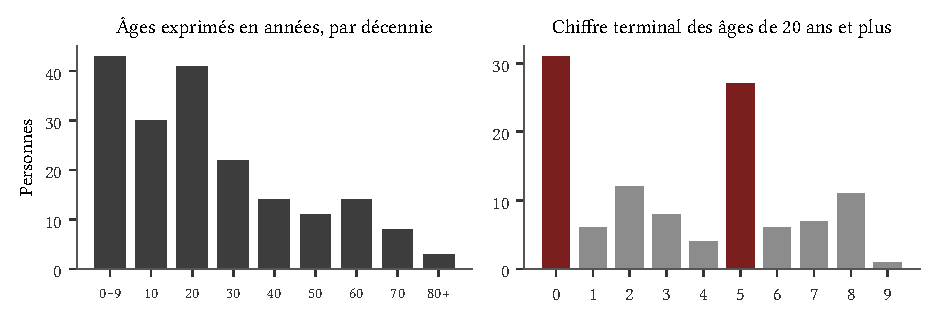
\includegraphics[width=\linewidth]{figures/fig_ages.pdf}
\caption{À gauche : âges exprimés en années, par décennie (ensemble C, n = \st{nAgeAns}). À droite : chiffre terminal des âges de vingt ans et plus (n = \st{nAges20}) ; en rouge, 0 et 5.}\label{fig:ages}
\end{figure}

Ces nombres ne mesurent pas la mortalité. La commémoration épigraphique sélectionne les défunts selon l’âge, le sexe, le statut et la famille ; les enfants y sont surreprésentés par rapport aux adultes âgés, et la part des jeunes enfants commémorés ne peut être assimilée à leur poids démographique. Les travaux de Hopkins, de Shaw et de Scheidel (chapitre~\ref{ch:historiographie}) interdisent de tirer de ces chiffres une espérance de vie.

\section{L’arrondi des âges}

L’attraction des âges ronds est très marquée. Sur les \st{nAges20} âges de vingt ans et plus, 31 se terminent par 0 et 27 par 5 : plus de la moitié, alors qu’une déclaration exacte en donnerait environ un cinquième. Pour les âges de 23 à 62 ans, l’indice de Whipple atteint \st{whipple} (\st{whippleN} personnes) et \st{whippleLu} pour les seuls âges entièrement lus (\st{whippleLuN} personnes) ; la valeur 100 correspond à l’absence d’attraction, 500 à une déclaration exclusivement en multiples de cinq. L’expression \emph{plus minus}, présente pour \st{nPlusMinus} personnes, va dans le même sens : pour une part notable des adultes, l’âge gravé est une estimation, et le texte le dit.

À l’inverse, la précision au mois et au jour se rencontre surtout pour les enfants. Un seul texte donne une durée en heures sans restitution : Ianuaria a vécu 24 ans, un jour et deux heures et demie (\emph{annos XXIIII diem I horas II s(emis)}, \nnum{118}). Aux \nnums{287} et 305, la mention des heures est restituée.

\section{La vie conjugale}

Vingt-trois textes indiquent la durée de la vie commune, souvent avec la même précision que l’âge (\emph{fecit cum marito annos…}, \emph{vixit mecum…}, \emph{in coniugio fecit…} ; tableau~\ref{tab:conjugale}). Lorsque l’âge et la durée du mariage sont tous deux conservés, ils permettent d’estimer l’âge au mariage. Sabina, morte à quinze ans, a été mariée deux ans (\nnum{200}) ; Paternia, morte « à environ quarante ans », vingt ans (\nnum{223}) ; Caelestina, morte à vingt ans, quatre ans (\nnum{399}). Le \nnum{324} distingue en outre les fiançailles : Hilaritas, fiancée à onze ans, le reste sept ans, puis vit sept ans et huit mois avec son mari ; le mariage a donc eu lieu vers dix-huit ans, et la somme (25 ans et 8 mois) concorde avec l’âge gravé, \emph{ann(os) XXV}.

% généré par scripts/04_generated.py
\begin{longtable}{@{}r r p{0.75\linewidth}@{}}\caption{Durées de vie commune déclarées (ensemble C ; extrait du texte transmis).}\label{tab:conjugale}\\\toprule N° & Année & Passage\\\midrule\endfirsthead\bottomrule\endfoot
4 & 341 & \lat{⸢v⸣ixit / cum ⸢v⸣(i)rg(i)nia annis XV bene merenti ⸢v⸣irginia sua Bictora /} \\
21 & 347 & \lat{fecit cum m[arito annos / quae vixit a]nn(os) XXXV m(enses) II d(ies)} \\
26 & 348 & \lat{vixit mecum / annos XVIII m(enses) V d(ies) XXV Aradius} \\
40 & 353 & \lat{⸢v⸣ix⸢i⸣t cum co/[niuge sua annos] XXI me(n)s(es) III depositus / [annoru]} \\
53 & 358 & \lat{vixit cum marito / [annos] m(enses) VIII} \\
83 & 364 & \lat{fecit [mecum] / m(enses) VI d(ies) XXII dep(osita) in p(ace)} \\
135 & 369 & \lat{fecit mecum a(n)n(os) XV / [Va]lentiniano ⸢d⸣(omino) n(ostro)} \\
184 & 375 & \lat{fecit cum co⸢m⸣pare suo m(enses) X d(ies) V / Kal(endis) No⸢v⸣(embribus)} \\
185 & 375 & \lat{fecit mecum annos XX} \\
193 & 376 & \lat{fecit cum marito ann⸢o⸣s plus minus quin/decim et dies duodecim} \\
200 & 377 & \lat{in coniu(gio) fec(it) ann(os) II} \\
219 & 381 & \lat{vixit cu[m marito suo] / IIII ⸢F⸣l(avio) Sy[agrio]} \\
223 & 381 & \lat{fecit cu/m marito suo an(nos) XX / discessit pri(die) Kal(endas) /} \\
254 & 383 & \lat{[fecit c]um marit[o annos] / Merob[aude II et Saturnino conssulibu]} \\
265 & 384 & \lat{fecit cum virginio suo an[nos / Rico]mere et Clearcho consulib} \\
286 & 386 & \lat{fecit cum vi[rginia sua annos consu]/latu Honori[o nobilissimo pu]} \\
291 & 387 & \lat{[fecit cum ma]rit⸢o⸣ ann[os] dies X [recessit / in pace K]al(endas) Ia} \\
324 & 390 & \lat{vixit cum marito ann(os) VII menses VIII deposita die XVII Kal(en)} \\
364 & 394 & \lat{fec⸢i⸣t / [cum coniuge s]ua Donata dulcissima / [annos quinqu]e depos} \\
365 & 394 & \lat{fecit / cum co⸢m⸣pare sua ann⸢o⸣s septe(m) / mens⸢e⸣s VIIII bene merent} \\
373 & 395 & \lat{fecit cum [marito suo annos] / dies III deposita / conss(ulib)} \\
399 & 397 & \lat{fecit cum marito annos V d(ies) VI / deposita IIII Non(as) Iul(ias)} \\
420 & 398 & \lat{fecit cu[m coniuge suo] / d(ies) LXX in p(ace)} \\
\end{longtable}


L’emploi de \emph{virginius} et de \emph{virginia} pour désigner l’époux ou l’épouse épousé vierge est attesté sans restitution dans trois textes (\nnums{4}, 218 et 265) et restitué dans deux autres (\nnums{45} et 286). Au \nnum{4}, Iunianus a vécu quinze ans « avec sa \emph{virginia} » Victora (\emph{Bictora}), qui fait graver l’épitaphe ; les deux époux sont qualifiés d’\emph{amator} et d’\emph{amatrix pauperum}. Ce vocabulaire appartient aux épitaphes chrétiennes de Rome ; il valorise le mariage unique, sans permettre d’en mesurer la fréquence.

\section{Les enfants}

Les épitaphes d’enfants ont un vocabulaire propre. \emph{Innocens}, \emph{innox} et \emph{dulcissimus} qualifient l’enfant ; \emph{puer} et \emph{puella} sont employés jusqu’à l’adolescence (Ursa, \emph{puella} de vingt-deux ans, au \nnum{411} ; Sabina, \emph{puella} mariée, au \nnum{200}). Deux enfants sont dits \emph{neofytus} : Aristo, mort à huit mois (\nnum{308}), et Quiminatus, mort à environ cinq ans (\nnum{210}). Ces deux textes attestent le baptême d’enfants jeunes, peut-être administré à l’approche de la mort ; ils sont repris au chapitre~\ref{ch:foi_eglise}.

\chapter{Rangs, fonctions et origines}\label{ch:rangs}

\section{Le clarissimat des défunts}

La première version du catalogue réunissait sous la rubrique « \emph{clarissimus} » la titulature des consuls, \emph{v(iri) c(larissimi)}, et le rang des personnes commémorées. Les deux sont désormais séparés. La titulature apparaît dans environ quatre-vingt-dix textes de l’ensemble C, presque toujours dans la formule consulaire. Le rang sénatorial d’une personne commémorée ou d’un commanditaire n’est attesté que dans onze textes : \nnums{15}, 19, 36, 44, 179, 213, 262, 306, 330, 430 et 452.

Ces onze textes forment un groupe hétérogène. Cassia Pisonis, \emph{c(larissima) f(emina)}, dont l’épitaphe est gravée sur un sarcophage, est née en 316 et morte en 346 (\nnum{15}). Au \nnum{179}, une même dalle commémore Simplicius, \emph{v(ir) c(larissimus)}, Didyme et Roscia Calchedonia, \emph{c(larissimae) f(eminae)}, et Innocentius, \emph{[dormi]entes in pace} (participe en partie restitué). Au \nnum{213}, Eustolius, \emph{v(ir) c(larissimus)}, repose avec sa fille. Egnatia Susanna, dite aussi Abita, est une \emph{c(larissima) p(uella)} morte à cinq ans (\nnum{330}). Les autres textes sont fragmentaires (\nnums{44}, 262, 430, 452).

Deux textes posent des questions d’identification.

\emph{Le \nnum{36}.} Clodius Adelfius, \emph{v(ir) c(larissimus) ex praefectis urbis}, fait graver l’épitaphe de son « épouse incomparable » et la sienne. La bibliographie l’identifie habituellement à Clodius Celsinus Adelphius, préfet de la Ville en 351 et époux de la poétesse chrétienne Faltonia Betitia Proba. L’identification est vraisemblable mais n’a pas été contrôlée sur la \emph{Prosopography of the Later Roman Empire}. Elle est en tout cas la seule source de l’année : le texte ne contient aucune date, et l’année 351 de la base est un terme postérieur, non l’année du décès (chapitre~\ref{ch:fondement}).

\emph{Le \nnum{306}.} Lucceia, \emph{c(larissima) f(emina)}, est dite fille de Viventius, \emph{c(larissimae) r(ecordationis) v(ir) ex praefecto praetorio et urbis aeternae}. L’identification de ce Viventius au préfet de la Ville de la fin des années 360 relève de la même vérification prosopographique. Lucceia fait ensevelir dans son propre sarcophage la vierge Maximilla, originaire de Pannonie, « par amitié », avec la mère de celle-ci, Nunita, \emph{matrona diaconi} (chapitre~\ref{ch:textes_decisifs}).

\section{Clercs, fonctions et métiers}

Le tableau~\ref{tab:fonctions} réunit les mentions de fonctions ecclésiastiques, de charges et de métiers. Le relevé porte sur l’ensemble B, qui comprend les actes d’achat, et sur la colonne de Saint-Paul (\nnum{321}). L’astérisque signale une attestation dont le mot est entièrement restitué.

% généré par scripts/04_generated.py
\begin{table}[tbp]\centering\small\caption{Fonctions, rangs et métiers mentionnés (ensemble B et \nnum{321} ; l’astérisque signale une attestation seulement restituée). Le rang n’est pas toujours celui du défunt.}\label{tab:fonctions}
\begin{tabular}{@{}l r p{0.5\linewidth}@{}}\toprule Terme & Textes & Notices\\\midrule
\lat{lector} & 4 & 67*, 202, 269, 421 \\
\lat{presbyter} & 8 & 93*, 105, 134, 289*, 310, 378, 387*, 428* \\
\lat{diaconus} & 3 & 134, 306, 378 \\
\lat{episcopus} & 4 & 321, 378, 387, 400 \\
\lat{fossor} & 4 & 209, 217, 424, 478 \\
\lat{medicus} & 1 & 296 \\
\lat{pictor} & 1 & 229* \\
\lat{numerarius} & 1 & 429 \\
\lat{scholasticus} & 1 & 469 \\
\lat{quadratarius} & 1 & 189* \\
\lat{armararius} & 1 & 365 \\
\lat{praefectus} & 3 & 36, 72, 306 \\
\lat{praeses (ex praesidibus)} & 1 & 20 \\
\lat{tribunus} & 1 & 321* \\
\lat{sacerdos} & 1 & 289* \\
\lat{matrona (diaconi, presbyteri)} & 3 & 306, 378*, 428 \\
\bottomrule\end{tabular}\end{table}


\emph{Les lecteurs.} Trois lecteurs sont rattachés à une église de la Ville : Cinnamius Opas, \emph{lector tituli Fasciolae}, mort à 46 ans en 377 (\nnum{202}) ; Leopardus, \emph{lector de Pudentiana}, mort à 24 ans en 384 (\nnum{269}) ; Pascentius, \emph{lector de Fasc[iola]}, mort à 21 ans en 398 (\nnum{421}). Un quatrième, Iulius Innocentius, est dit \emph{lect[or] ec(c)les[iae sanctae c]at(h)olic(a)e} et serait mort à 73 ans en 362 (\nnum{67}) ; mais le mot \emph{lector} est en partie restitué, et l’expression \emph{ecclesiae sanctae catholicae} l’est presque entièrement. Ces âges montrent que la fonction de lecteur n’est pas réservée aux jeunes gens. Cinnamius Opas est en outre qualifié d’\emph{amicus pauperum}.

\emph{Prêtres, diacres et évêques.} Le \nnum{134} commémore un prêtre, Dulcitius, et un diacre, Gregorius, frères, avec leur sœur. Le \nnum{310} est l’épitaphe qu’un prêtre, Gaudentius, fait graver pour lui-même et pour son épouse Severa, \emph{casta}. Au \nnum{428}, Remigia, \emph{matrona} du prêtre Laurentius, fait graver son épitaphe ; mais le titre de Laurentius n’est conservé que par les lettres \emph{[p]r(es)b(yter)}, et la mention de l’\emph{ecclesia catholica} est restituée. Au \nnum{306}, Nunita est \emph{matrona diaconi} : l’EDCS supprime le S final gravé (\emph{diaconi\{s\}}), et la lecture « épouse d’un diacre » dépend de cette correction. Ces textes documentent l’ancrage familial du clergé romain et le mariage des clercs à la fin du \textsc{iv}\textsuperscript{e} siècle.

Le \nnum{378} développe une généalogie cléricale : à la suite du père, le prêtre Limenius, le texte énumère une série d’ascendants et de parents (\emph{nepos}, \emph{pronepos}, \emph{abnepos}, \emph{socrus}) parmi lesquels un diacre de la cinquième région, un évêque Marcellus, une \emph{matrona presbyteri} et un évêque Ursinus d’Albano. La structure exacte de cette généalogie dépend de nombreuses restitutions. Surtout, elle n’est transmise que par l’EDCS : aucune des fiches de l’EDB rattachées au monument ne la contient (chapitre~\ref{ch:evenements}). Elle doit être contrôlée sur l’ICVR III 8345 avant toute exploitation prosopographique.

Trois mentions d’évêques concernent l’évêque de Rome ou un évêque dont l’identité est discutée. Sur la colonne de Saint-Paul, \emph{Siricius episcopus tota mente devotus} (\nnum{321}, non funéraire) atteste l’intervention de l’évêque dans la construction de la basilique. Au \nnum{387}, la formule \emph{sub episcopatu Si[rici]} est en grande partie restituée, de même que l’emplacement \emph{[ad limina Petri et] Pauli}. Au \nnum{400}, l’emplacement a été acheté par Viricunda, épouse du défunt, \emph{Pascasio ep(is)c(opo)} ; l’EDB reprend la note de Diehl selon laquelle aucun évêque de Rome ne porte ce nom. La fonction de ce Pascasius dans la transaction reste indéterminée (chapitre~\ref{ch:sepultures}).

\emph{Charges et métiers.} Le \nnum{20} commémore Flavius Gaianus, \emph{ex praesidibus}, ancien gouverneur de province. Le \nnum{429} nomme Martielis, \emph{numerarius vicariae sedis urbis Romae aeternae}, comptable de l’administration du vicaire de la Ville. Le \nnum{469} mentionne deux \emph{scholastici}. Le \nnum{296} est l’épitaphe de Rapetiga, médecin, \emph{civis Hispanus}, mort à environ 25 ans. Un peintre (\emph{pict[or]}, \nnum{229}) et un \emph{[qua]dratarius} (\nnum{189}) sont attestés par des mots en partie restitués. Les \emph{fossores} apparaissent uniquement comme vendeurs d’emplacements (\nnums{209}, 217, 424 et 478 ; chapitre~\ref{ch:sepultures}).

\section{Dater par le préfet de la Ville}

Le \nnum{72} associe à la formule consulaire de 362 (\emph{Mamertino et Nevitta conss.}) la mention du préfet de la Ville, \emph{pr(a)ef(ecto) urb(i) Maximo}. Cette double datation, exceptionnelle dans le corpus, appartient à un texte qui commence par \emph{D(is) M(anibus) s(acrum)} et se poursuit par \emph{requievit in pace} : la formule païenne traditionnelle et la formule chrétienne coexistent sur la même plaque (chapitre~\ref{ch:mort_esperance}).

\section{Origines déclarées}

Quelques défunts sont présentés par leur origine : Quirillus, \emph{civis Armeniacus Cappadox} (\nnum{275}) ; Rapetiga, \emph{civis Hispanus} (\nnum{296}) ; Maximilla, \emph{civis Pannonia} (\nnum{306}, ligne dont la présence doit être contrôlée sur l’édition, car elle manque dans le texte de l’EDB) ; Vitalia, \emph{εὐγενεστάτη Κωνσταντινουπολίτισσα} (\nnum{168}, en partie restitué) ; Alexandros, du village de Mikra Kômè (\nnum{348}) ; selon l’EDB, un originaire de Théodosiopolis (\nnum{447}, restitué). Au \nnum{19}, Flavius Aurelius Casarius, dit Santulus, est venu de Préneste à Rome, où il a vécu vingt-deux jours ; l’indication \emph{[ante annos d]uos} est restituée. Le \nnum{183} situe la défunte, Petronia, \emph{virgo}, dans la neuvième région de la Ville, \emph{a lacu cunic(u)li} ; la localisation de ce repère relève de la topographie romaine et n’est pas proposée ici.

Ces mentions sont rares et ne permettent aucune estimation de la part des immigrés dans la population chrétienne. Elles montrent seulement que l’origine est parfois jugée digne d’être gravée, surtout pour des personnes venues de loin.

\chapter{Anthroponymie}\label{ch:noms}

Le relevé des noms n’est pas une prosopographie. Une forme peut appartenir à un défunt, à un commémorant, à un consul, à un vendeur d’emplacement ou à une personne citée dans une généalogie ; les changements de cas, les abréviations et les restitutions compliquent la reconnaissance. L’index des noms (chapitre~\ref{ch:index}) est produit automatiquement à partir du texte transmis : il retient les mots à initiale capitale, écarte les noms consulaires de l’année du texte et de l’année précédente (sauf lorsqu’ils désignent une autre personne), les noms de mois et de jours, et signale d’un astérisque les formes dont une lettre au moins est restituée. Il donne les formes telles qu’elles sont gravées, sans lemmatisation. Il reste un instrument de repérage.

\section{Gentilices et noms uniques}

La plupart des personnes commémorées portent un nom unique. Les gentilices sont rares et concentrés dans quelques familles ou quelques milieux. Hors des formules consulaires, \emph{Flavius} et \emph{Flavia} sont les plus fréquents (\nnums{19}, 20, 57, 59, 72, 149, 157, 217, 221 et 440), ce qui reflète la diffusion de ce nom, devenu presque un titre, dans le service impérial du \textsc{iv}\textsuperscript{e} siècle. \emph{Aurelius} et \emph{Aurelia} viennent ensuite (\nnums{6}, 19, 23, 111 et 229). Les autres gentilices n’apparaissent qu’une ou deux fois, souvent dans les textes de rang sénatorial : Cassia (\nnum{15}), Clodius (\nnum{36}), Roscia (\nnum{179}), Egnatia (\nnum{330}), Lucceia (\nnum{306}), Statilia (\nnum{42}), Cornificia (\nnum{77}), Aufidia (\nnum{449}), Valerius (\nnum{262}).

Ces effectifs ne mesurent ni la citoyenneté juridique ni la structure sociale de la population chrétienne : l’abandon du gentilice dans les épitaphes est un fait de pratique, non un indice de statut servile.

\section{Noms à signification chrétienne}

Un petit nombre de noms a une signification chrétienne directe ou probable : Adeodata (\nnum{297}) et peut-être Adeoda[tus] (\nnum{378}, restitué), Quodvultdeus (\nnum{388} ; \emph{Quodvuldeus} au \nnum{112}, en partie restitué), Theodora (\nnum{80}), Theodotus (\nnum{5}), Theophila (\nnum{110}), Anastasius et Anastasia (\nnums{43}, 195 et 197), Benedictus (\nnums{268} et 441), Martyrius (\nnum{139}), Pascasius (\nnums{235} et 400), Quiriace, c’est-à-dire Κυριακή (\nnum{298}). D’autres renvoient à des figures bibliques ou apostoliques (Petrus, \nnum{197} ; Paulus, \nnum{398} ; le Ioannes du \nnum{261}, gravé \emph{Ioannti}), ou au sabbat (Sabbatius, \nnums{22} et 386 ; Sambatia, \nnum{339}). Le nom \emph{Stercoria} (\nnum{108}, en partie restitué) appartient au groupe des noms d’humilité, dont Kajanto a montré la fréquence dans les inscriptions chrétiennes.\footnote{I.~Kajanto, \emph{Onomastic Studies in the Early Christian Inscriptions of Rome and Carthage}, Helsinki, 1963 (Acta Instituti Romani Finlandiae, II, 1) ; Ch.~Pietri, « Remarques sur l’onomastique chrétienne de Rome », dans \emph{L’onomastique latine}, Paris, 1977. Notices bibliographiques reprises de la bibliographie du volume ; passages non consultés.}

Ces noms ne sont pas des professions de foi. Leur analyse étymologique peut éclairer un horizon culturel ; mais le nom peut avoir été donné bien avant l’événement commémoré, relever d’une transmission familiale ou d’un usage devenu banal. La date d’une épitaphe atteste l’emploi d’un nom à cette date, non la date de son attribution, et l’usage d’un nom à étymologie chrétienne ne suffit pas à établir l’identité religieuse de son porteur. Inversement, la très grande majorité des défunts du corpus porte des noms latins ou grecs traditionnels (Felix, Victor, Leo, Laurentius, Ursus, Ianuaria, Crescentia…), sans signification chrétienne particulière.

\section{Doubles noms et désambiguïsation}

La formule \emph{Muscula quae et Galatea} (\nnum{151}) signale explicitement un double nom ; de même, \emph{Egnatia Susanna} est dite aussi \emph{Abita} (\nnum{330}), et Flavius Aurelius Casarius porte le surnom de \emph{Santulus} (\nnum{19}). Ces formulations doivent être distinguées des rapprochements entre deux fiches portant des noms voisins. L’identité d’une personne ne se déduit ni d’un nom commun ni d’une date proche : elle suppose la convergence d’indices documentaires. Les identifications proposées dans les dossiers commentés (Clodius Adelfius, Viventius, Proiecta) demeurent des hypothèses tant qu’elles n’ont pas été vérifiées dans la \emph{Prosopography of the Later Roman Empire} et la \emph{Prosopographie chrétienne du Bas-Empire} ; une référence à ces instruments désigne alors un contrôle à effectuer, non la preuve que ce contrôle a eu lieu.

\chapter{Relations familiales et commémorants}\label{ch:relations}

Les termes de parenté et de relation désignent, selon les textes, la personne commémorée ou celle qui commémore. Le relevé ci-dessous ne les distingue pas automatiquement : il fournit pour chaque terme l’effectif des textes de l’ensemble C, le nombre de textes où le terme est lu sans restitution, la répartition par période de ces derniers et la liste des notices (tableau~\ref{tab:relations}).

% généré par scripts/04_generated.py
\begin{table}[tbp]\centering\small\caption{Termes de parenté et de relation dans l’ensemble C (textes, non occurrences) : attestations restitutions comprises, attestations lues, et répartition des attestations lues par période.}\label{tab:relations}
\begin{tabular}{@{}l r r r r r r@{}}\toprule Terme & Total & Lu & 340–359 & 360–374 & 375–389 & 390–403\\\midrule
\lat{coniux, compar} & 39 & 22 & 5 & 4 & 7 & 6 \\
\lat{maritus} & 27 & 19 & 5 & 5 & 6 & 3 \\
\lat{uxor} & 12 & 8 & 3 & 4 & 0 & 1 \\
\lat{filius, filia} & 33 & 27 & 3 & 9 & 9 & 6 \\
\lat{pater} & 9 & 8 & 2 & 1 & 5 & 0 \\
\lat{mater} & 8 & 8 & 0 & 3 & 1 & 4 \\
\lat{parentes} & 12 & 8 & 2 & 3 & 1 & 2 \\
\lat{frater} & 6 & 4 & 0 & 1 & 1 & 2 \\
\lat{soror} & 4 & 3 & 1 & 0 & 1 & 1 \\
\lat{nepos, neptis} & 1 & 0 & 0 & 0 & 0 & 0 \\
\lat{amicus, amica} & 7 & 6 & 1 & 1 & 3 & 1 \\
\lat{socrus, gener, nurus} & 3 & 3 & 1 & 0 & 0 & 2 \\
\lat{virginius, virginia} & 5 & 3 & 1 & 0 & 2 & 0 \\
\bottomrule\end{tabular}\end{table}


\section{Le couple au centre de la commémoration}

Les termes conjugaux (\emph{coniux}, \emph{compar}, \emph{maritus}, \emph{uxor}, \emph{virginius}) dominent nettement les autres relations. La commémoration d’un conjoint par l’autre est la configuration la plus fréquente parmi les textes qui nomment un commanditaire : Agrippina pour Felix (\nnum{133}), Theophila pour Benenatus (\nnum{110}), Constantia pour Anastasius (\nnum{43}, en partie restitué), Victora pour Iunianus (\nnum{4}), Aradius Melissus pour Esuvia Ianuaria (\nnum{26}), Sabbatius pour Staturina (\nnum{386}), Viricunda pour Severianus (\nnum{400}). Plusieurs textes associent le commanditaire à la sépulture : Marcus fait pour Karisia et pour lui-même une « demeure éternelle » (\emph{feci nobis domum aeternalem}, \nnum{46}) ; le prêtre Gaudentius grave l’épitaphe de son épouse et la sienne (\nnum{310}) ; Clodius Adelfius fait de même (\nnum{36}).

La part des textes qui mentionnent un terme conjugal décroît au cours de la période (chapitre~\ref{ch:formulaire}). Il n’est pas possible de dire si ce recul traduit un changement des pratiques de commémoration, une modification de la composition sociale ou topographique du corpus, ou l’état de conservation des textes les plus tardifs.

\section{Parents et enfants}

Les parents commémorent leurs enfants, le plus souvent sans être nommés (\emph{parentes fecerunt}, \emph{parentes filio dulcissimo}) : Cheretius et Severa pour leur fils Cheretius, mort à cinq ans (\nnum{17}) ; les parents de Successa, morte à deux ans (\nnum{35}) ; les « malheureux parents » du \nnum{93}. Les termes \emph{mater} et \emph{pater} désignent tantôt la personne commémorée (Eleuteria, pour qui son fils Pacatianus fait un emplacement, \nnum{73} ; Nunita, mère de Maximilla, \nnum{306}), tantôt le commanditaire (le père Eutyches, \nnum{68} ; le père Nicetius, \nnum{296} ; « la mère et le père » de Felicitas, \nnum{470}). L’épitaphe de Proiecta (\nnum{244}), due à l’évêque Damase, nomme le mari, Primus, la mère et le père, Florus.

Le \nnum{399} réunit, sur une même plaque, Caelestina, épouse d’Ampliatus, morte à vingt ans, et Hilaritas, \emph{filia} morte à vingt-trois ans, qui ne peut donc être la fille de Caelestina ; toutes deux étaient mariées, et elles sont mortes à quelques semaines d’intervalle ; le \nnum{134}, un prêtre, un diacre et leur sœur. Ces textes à plusieurs défunts sont des documents familiaux autant que funéraires.

\section{Au-delà de la famille}

L’amitié est rarement invoquée, mais elle peut fonder une sépulture. Lucceia ensevelit dans son propre sarcophage la vierge Maximilla, \emph{propter amicitiam sibi coniunctam} (\nnum{306}). Cinnamius Opas, lecteur, et les époux du \nnum{4} sont dits « amis des pauvres » (\emph{amicus}, \emph{amator}, \emph{amatrix pauperum}) ; Quirillus, « aimé de tous » (\emph{omnibus amicatus}, \nnum{275}). Dans les textes où ils sont lus, les termes \emph{frater} et \emph{soror} se comprennent naturellement comme des liens de parenté (Priscus pour sa sœur, \nnum{132} ; deux frères qui se préparent une sépulture de leur vivant, \nnum{441}) ; rien n’y indique un emploi ecclésial.

% généré par scripts/04_generated.py
\begin{small}\noindent \lat{coniux, compar} : 1, 10, 13, 19, 26, 28, 33, 40, 43, 46, 47, 49, 83, 115, 117, 125, 130, 147, 184, 200, 242, 262, 275, 288, 304, 306, 310, 319, 320, 324, 333, 364, 365, 378, 382, 399, 420, 455, 472.\par\noindent \lat{maritus} : 21, 26, 29, 32, 42, 53, 77, 82, 114, 125, 133, 144, 184, 185, 193, 219, 223, 244, 254, 257, 291, 297, 324, 373, 386, 399, 454.\par\noindent \lat{uxor} : 10, 23, 34, 36, 43, 56, 104, 110, 146, 167, 400, 438.\par\noindent \lat{filius, filia} : 6, 13, 35, 42, 59, 64, 68, 81, 84, 92, 99, 100, 127, 143, 186, 196, 211, 213, 221, 233, 259, 268, 297, 306, 309, 347, 353, 378, 399, 402, 412, 431, 457.\par\noindent \lat{pater} : 2, 22, 68, 203, 241, 268, 296, 297, 378.\par\noindent \lat{mater} : 73, 81, 102, 306, 353, 382, 461, 470.\par\noindent \lat{parentes} : 17, 35, 64, 74, 93, 124, 126, 152, 189, 244, 409, 439.\par\noindent \lat{frater} : 132, 247, 314, 368, 441, 457.\par\noindent \lat{soror} : 12, 134, 181, 469.\par\noindent \lat{nepos, neptis} : 378.\par\noindent \lat{amicus, amica} : 22, 133, 189, 202, 214, 268, 391.\par\noindent \lat{socrus, gener, nurus} : 48, 378, 382.\par\noindent \lat{virginius, virginia} : 4, 45, 218, 265, 286.\end{small}



\part{Pratiques funéraires et mémoire chrétienne}
\chapter{Méthode : une typologie textuelle du vocabulaire religieux}\label{ch:typologie}

\section{Pourquoi abandonner le profil unique}

Le catalogue de travail attribuait à chaque épitaphe un profil thématique unique (« aucune mention divine », « Dieu », « Christ », « Esprit saint », « binaire », « trinitaire explicite », « initiation et foi », « appartenance ecclésiale »), selon la catégorie la plus spécifique présente dans le texte. Ce codage avait le mérite de la clarté, mais il présentait deux défauts. Il ne distinguait pas le statut textuel des mots : un \emph{Christi} entièrement restitué par l’éditeur et un \emph{Chr(isti)} gravé en abrégé recevaient la même valeur. Et il projetait sur certains textes une structure doctrinale qu’ils ne contiennent pas : le \nnum{474}, qui dit seulement \emph{confirmans trinitatem}, était codé « trinitaire explicite (Père, Fils, Esprit) » ; le \nnum{458}, qui dit \emph{ancilla dei et Chr(isti)}, « binaire (Père et Fils) ».

La présente édition remplace ce profil par un relevé de chaque occurrence, qualifiée selon deux axes indépendants, et confronte ce relevé à une recherche lexicale indépendante menée sur l’ensemble du texte transmis.

\section{Premier axe : le statut textuel}

Quatre valeurs décrivent la transmission d’un mot : 1, mot lu ; 2, abréviation développée par l’éditeur ; 3, restitution partielle ; 4, restitution intégrale. Une marque distincte, S, désigne un signe figuré décrit par un témoin (monogramme du Christ). Deux codes hérités, 5 (« allusion ») et 6 (« anthroponyme »), décrivent une interprétation ou une fonction, non un état de conservation ; ils sont conservés pour la traçabilité, mais ne prolongent pas l’échelle philologique.

Une désignation divine n’est retenue indépendamment des restitutions que si l’élément conservé, ou une abréviation suffisamment déterminée, porte lui-même l’identification religieuse. Au \nnum{249}, \emph{spiritum} est lu, mais l’identification de l’Esprit saint dépend de la restitution partielle de \emph{[sanc]tum} ; au \nnum{352}, \emph{[qui Ch]ristum credens}, la fin du nom est lue mais son début restitué. Ces textes ne sont comptés qu’avec les restitutions.

Le niveau 1 ne certifie pas une lecture nouvellement collationnée sur la pierre : il signifie que les deux bases, ou la seule base disponible, transmettent le mot sans crochets. Lorsque l’EDB souligne des lettres, signe que ces lettres ont été lues par des éditeurs antérieurs mais ne sont plus visibles, la notice le signale (ainsi \emph{domino} au \nnum{85}).

\section{Second axe : l’emploi}

Chaque occurrence reçoit une catégorie d’emploi : désignation de Dieu, désignation du Christ, Esprit saint, Trinité, initiation et foi, vocabulaire ecclésial, saints, intercession, résurrection, repos et sommeil, allusion, anthroponyme. La catégorie dépend du contexte immédiat et a été attribuée par des règles explicites, contrôlées à la lecture : \emph{sanctum} suivi de \emph{spiritum} relève de l’Esprit saint ; \emph{sanctis} ou \emph{sanctorum} employés substantivement relèvent des saints ; \emph{sanctus} qualifiant un défunt est une épithète ; \emph{spiritus} désignant l’esprit du défunt relève de l’anthropologie. La titulature impériale \emph{dominus noster} est exclue, de même que \emph{dominus} au sens de maître (\emph{Cecili dominus Felicis}, \nnum{102}).

\section{Contrôle par une recherche indépendante}

Le relevé de la base de travail a été confronté à une recherche par expressions régulières sur le texte transmis de l’ensemble C, pour une trentaine de familles de mots (\emph{deus}, \emph{dominus}, \emph{Christus}, \emph{spiritus}, \emph{sanctus}, \emph{trinitas}, \emph{fides}, \emph{credere}, \emph{neophytus}, \emph{baptisma}, \emph{ecclesia}, \emph{martyr}, \emph{resurrectio}, \emph{caelum}, \emph{lux}, \emph{paradisus}, \emph{refrigerium}, \emph{anima}, \emph{gratia}, \emph{peccatum}, \emph{redemptus}, \emph{spes}, \emph{orare}…). Elle confirme le relevé pour les désignations divines. Elle fait apparaître des absences significatives : aucun texte latin de l’ensemble ne contient les mots \emph{Iesus}, \emph{baptisma}, \emph{martyr}, \emph{resurrectio}, \emph{paradisus}, \emph{gratia} ou \emph{peccatum}, même restitués. Elle conduit enfin à corriger trois classements :

\begin{itemize}
\item au \nnum{152}, la lecture \emph{redemptus}, qui fondait une allusion à la rédemption, n’est pas celle de l’EDB, qui lit \emph{[cor]p⟨o⟩re demptus} ; l’occurrence est retirée ;
\item au \nnum{447}, le mot \emph{ἀναστάσεως} est une restitution de l’EDCS, assortie d’un point d’interrogation, que l’EDB remplace par \emph{κρίσεως} ; il n’y a donc pas de mention de la résurrection assurée dans le corpus (chapitre~\ref{ch:mort_esperance}) ;
\item au \nnum{73}, la crainte de Dieu (\emph{[quaeque deu]m metuisti}) est une restitution de l’EDCS que l’EDB ne partage pas ; la désignation de Dieu du texte repose sur \emph{deo dica⟨vi⟩sti}, lu dans les deux bases.
\end{itemize}

\section{Résultats : trois profils de lecture}

Le tableau~\ref{tab:profils} réunit les dix-neuf textes de l’ensemble C qui contiennent, sous une forme quelconque, une désignation de Dieu, du Christ, de l’Esprit ou de la Trinité. Trois règles de compte en sont tirées.

\begin{description}[style=nextline,leftmargin=1.5em,font=\normalfont\scshape]
\item[Profil large] Textes où au moins une désignation est lue ou abrégée (niveaux 1–2), le signe du \nnum{38} exclu : \st{nProfilLarge} textes sur \st{nC} (\st{pProfilLarge}~\%).
\item[Profil restrictif] Le même, sans les deux textes dont l’identification dépend d’un développement douteux ou d’une restitution (\nnums{232} et 249) : \st{nProfilRestr} textes (\st{pProfilRestr}~\%).
\item[Profil strict] Le même, sans les trois textes où l’abréviation \emph{Chr.} rend probablement un monogramme (\nnums{140}, 151 et 311) : \st{nProfilStrict} textes (\st{pProfilStrict}~\%).
\end{description}

Avec les restitutions, le total atteint \st{nProfilAvecRest} textes (+ \nnums{43}, 104, 352, 382 et 447). Ces comptes décrivent des catégories de lecture, non un taux d’adhésion doctrinale. Ils montrent que le résultat principal — la rareté des désignations divines dans les épitaphes datées — ne dépend pas de la règle adoptée : entre 1,7 et 3,9~\% des textes selon la règle la plus sévère et la plus généreuse.

\begin{table}[tbp]\centering\small
\caption{Désignations de Dieu, du Christ, de l’Esprit et de la Trinité dans l’ensemble C. Statut : 1 lu, 2 abrégé, 3 restitution partielle, 4 restitution intégrale, S signe. Profils : L large, R restrictif, S strict ; « rest. » : compté seulement avec les restitutions.}\label{tab:profils}
\begin{tabularx}{\linewidth}{@{}r r X l l@{}}\toprule
N° & Année & Formes (statut) & Remarque & Profils\\\midrule
38 & 352 & \lat{in pace} + monogramme (S) & EDCS : \lat{Chr(isti)} & —\\
43 & 355 & \lat{in nomine [Christi]} (4) & chrisme décrit & rest.\\
73 & 363 & \lat{deo dica⟨vi⟩sti} (1) ; \lat{[deu]m} (3, EDCS seul) & restitutions divergentes & L R S\\
85 & 364 & \lat{omnia domino} (1) & EDB : lettres vues jadis & L R S\\
104 & 366 & \lat{in pace d[ei?]} (3) & EDB : \lat{d[- - -]} & rest.\\
140 & 370 & \lat{in pace Chr(isti)} (2) & chrisme décrit & L R\\
151 & 371 & \lat{in pace Chr(isti)} (2) & chrisme décrit & L R\\
214 & 380 & \lat{ancilla dei} (1) & & L R S\\
232 & 382 & \lat{in dom(ino?)} (2?) & développement douteux & L\\
249 & 383 & \lat{[sanc]tum spiritum} (1 + 3) & & L\\
306 & 389 & \lat{vitam Cristi}, \lat{ancilla dei} (1) ; \lat{[foedera C]hristi} (3) & ligne à contrôler & L R S\\
311 & 388 & \lat{in Chr(isto)} (2) & chrisme décrit & L R\\
352 & 393 & \lat{[qui Ch]ristum credens} (3) & & rest.\\
382 & 395 & \lat{in sin[u dei]} (4) & & rest.\\
400 & 397 & \lat{in luce domini} (1) & monogrammes décrits & L R S\\
447 & 401 & \lat{[θεὸν τὸν παντο]κράτορα} (4 + 3) & & rest.\\
458 & 401 & \lat{ancilla dei et Chr(ist)i} (1 + 2) & CHRI gravé & L R S\\
474 & 403 & \lat{homo dei}, \lat{trinitatem} (1) & & L R S\\
475 & 403 & \lat{dedit deus deus tulit} (1) & & L R S\\\bottomrule
\end{tabularx}
\end{table}

Ces dix-neuf textes sont examinés dans les chapitres suivants : Dieu et le Christ (chapitre~\ref{ch:dieu_christ}), l’Esprit et la Trinité (chapitre~\ref{ch:esprit_trinite}). Le vocabulaire de la foi, de l’initiation et de l’Église (chapitre~\ref{ch:foi_eglise}) et celui de la mort et de l’espérance (chapitre~\ref{ch:mort_esperance}) relèvent d’autres catégories d’emploi. Le répertoire du chapitre~\ref{ch:rep_religieux} donne toutes les occurrences, avec leur statut et leur contexte.

\chapter{Dieu et le Christ dans les épitaphes}\label{ch:dieu_christ}

\section{Inventaire}

Dieu est désigné, sans restitution, dans huit textes de l’ensemble C, et peut-être dans un neuvième : \emph{deus} au \nnum{73} (\emph{deo dica⟨vi⟩sti}) et au \nnum{475} (\emph{dedit deus deus tulit}), \emph{ancilla dei} aux \nnums{214}, 306 et 458, \emph{homo dei} au \nnum{474}, \emph{dominus} aux \nnums{85} (\emph{omnia domino}) et 400 (\emph{in luce domini}), et peut-être au \nnum{232} (\emph{in dom(ino?)}). Le Christ est nommé en toutes lettres dans un seul texte (\emph{vitam Cristi}, \nnum{306}) ; il l’est sous une forme abrégée dans quatre autres (\emph{in pace Chr(isti)}, \nnums{140} et 151 ; \emph{in Chr(isto)}, \nnum{311} ; \emph{ancilla dei et Chr(ist)i}, \nnum{458}). Le nom de Jésus n’apparaît dans aucun texte.

Ces désignations sont donc à la fois rares et peu variées. Elles se répartissent en trois usages : la qualification du défunt (\emph{ancilla dei}, \emph{homo dei}), la formule du repos (\emph{in pace Christi}, \emph{in Christo}), l’éloge et la consolation.

\section{Le monogramme et le mot}

La formule \emph{in pace Christi} pose un problème de transcription que la confrontation des témoins rend visible. Au \nnum{38}, l’épitaphe de Privata (352), l’EDCS transcrit \emph{in pace Chr(isti)}, l’EDB \emph{in pace ((monogramma Christi))}, et l’estampage conservé dans la collection de l’Ohio State University sous le numéro ILCV 3252A montre un christogramme après IN PACE. Deux témoins indépendants de l’EDCS concordent : la pierre porte un monogramme, non le mot écrit en lettres.

Aux \nnums{140} et 151 (\emph{in pace Chr(isti)}) et au \nnum{311} (\emph{in Chr(isto)}), les deux bases transcrivent au contraire une abréviation, mais l’EDB décrit un chrisme parmi les données matérielles. Il est probable que, dans ces trois textes, le développement éditorial rende le même monogramme employé comme compendium du nom ; il n’est pas exclu qu’il s’agisse d’une abréviation en lettres accompagnée d’un chrisme décoratif. Seules les photographies permettraient de trancher. Au \nnum{458}, en revanche, l’EDB transcrit \emph{Chr(ist)i} : la lettre finale I est gravée, ce qui désigne une abréviation en lettres.

La différence n’est pas seulement philologique. Un monogramme employé comme abréviation fait partie de la phrase : \emph{in pace Christi} se lit, que le nom soit écrit en lettres ou en signe. Un monogramme juxtaposé n’appartient pas à la phrase : il marque le monument. Les profils du chapitre~\ref{ch:typologie} en tiennent compte en écartant ces quatre textes du profil strict.

\section{\emph{Ancilla dei}, \emph{homo dei} : qualifier la personne}

Trois textes qualifient une défunte d’\emph{ancilla dei} (\nnums{214}, 306 et 458 ; ce dernier avec \emph{ancilla dei et Chr(isti)}), un quatrième un défunt d’\emph{homo dei} (\nnum{474}). Ces expressions désignent l’appartenance de la personne à Dieu. Dans deux cas au moins, elles sont associées à la virginité : Maximilla, \emph{virgo ancilla dei} (\nnum{306}, ligne dont la présence doit être contrôlée sur l’édition, car elle manque dans le texte de l’EDB), et Praetiosa (\emph{Praetioso} dans l’EDCS), \emph{puella virgo XII tantum ancilla dei et Chr(isti)}, morte à douze ans (\nnum{458}). Au \nnum{474}, \emph{homo dei} ouvre une série de participes ascétiques (\emph{confirmans trinitatem}, \emph{amans castitatem}, \emph{respuens mundum}). Au \nnum{214}, l’\emph{ancilla dei} est une femme qui « a possédé cette maison de ses propres biens » et à qui l’on demande de prier pour l’enfant qu’elle laisse.

La formule \emph{ancilla dei et Chr(isti)} du \nnum{458}, que le catalogue de travail classait comme « binaire (Père et Fils) », associe Dieu et le Christ dans une formule de dévotion. Elle ne contient ni le mot « Père » ni le mot « Fils » et ne peut être tenue, sans argument supplémentaire, pour l’expression d’une doctrine des relations divines.

\section{Dieu dans l’éloge et dans l’épreuve}

Trois textes intègrent Dieu à un éloge ou à une consolation.

Le poème du \nnum{73} (363) loue Eleuteria, morte à environ 75 ans, qui « s’est toujours consacrée à Dieu » (\emph{quae te semper deo dica⟨vi⟩sti}, lu). La crainte de Dieu (\emph{[quaeque deu]m metuisti}) n’est qu’une restitution de l’EDCS, que l’EDB ne partage pas (\emph{[quaeque de]metuisti}).

Au \nnum{400} (397), l’esprit de Severianus « a été accueilli dans la lumière du Seigneur » (\emph{cuius spiritus in luce domini susceptus est}). La phrase est lue dans les deux bases, et l’EDB décrit sur la plaque un chrisme et deux croix monogrammatiques, dont l’une est placée immédiatement après \emph{susceptus est}.

Le \nnum{475} (403) reprend, sous une forme libre, la parole de Job : \emph{dedit deus, deus tulit}. La Vulgate porte \emph{Dominus dedit, Dominus abstulit} (Jb 1, 21) ; la forme épigraphique, avec \emph{deus} et \emph{tulit}, peut dépendre d’une version latine antérieure ou d’une citation de mémoire, ce que ce seul texte ne permet pas de décider.

\section{Le Christ dans les textes poétiques}

Deux textes poétiques nomment le Christ au-delà du formulaire. L’épitaphe de Maximilla (\nnum{306}, 389) commence par l’éloge d’une femme « capable de garder l’alliance du Christ » (\emph{poten[s servare foedera C]hristi}, restitution partielle), et poursuit : \emph{sed melius vivit vitam Cristi qui sperat aeternam}, « mais il vit mieux, celui qui espère la vie éternelle du Christ » (lu dans les deux bases). L’épitaphe d’Eutychius (\nnum{352}, 393) dit qu’« il possède la récompense de la lumière, croyant au Christ » (\emph{[qui Ch]ristum credens praemia lucis habet}) ; le début du nom est restitué, mais la fin \emph{-ristum} et le participe \emph{credens} sont lus.

\section{Ce que montrent ces textes}

Dans les épitaphes datées de 340–403, Dieu et le Christ sont nommés pour qualifier le défunt, pour situer son repos et pour consoler. Aucun texte ne développe un énoncé sur leur nature ou leur relation. Le Christ y est l’objet de la foi et le lieu du repos (\emph{in Christo}, \emph{in pace Christi}), le garant de la vie éternelle (\nnum{306}) et de la lumière promise (\nnum{352}). Cette pauvreté de l’énoncé ne permet aucune inférence sur la christologie des commanditaires : elle est d’abord un fait du genre épigraphique (chapitre~\ref{ch:rarete}).

\chapter{L’Esprit saint et la Trinité}\label{ch:esprit_trinite}

\section{Une seule mention possible de l’Esprit saint}

Le \nnum{249} est le seul texte de l’ensemble C qui puisse mentionner l’Esprit saint. Il s’agit d’un petit fragment de plaque (20 × 23,5 cm selon l’EDB), rattaché par l’EDB au cimetière de Nicomède, sur la via Nomentana. Les deux bases en donnent des transcriptions proches :

\begin{quote}\small
EDCS : \lat{[- - -]tus est qui ac[cepti sanc]tum spiritum [XVI Kal(endas)] Mai(as) Merobaud[e II con(sule)]}\\
EDB : \lat{tus est qui ac[cepit sanc]tum spirituṃ [XVI ? kal(endas)] mai(as) Merobaud[e consule]}
\end{quote}

Le mot \emph{spiritum} est lu, la dernière lettre étant pointée par l’EDB. De l’adjectif ne subsiste que la finale \emph{-tum} ; la restitution \emph{[sanc]tum} est vraisemblable, mais d’autres adjectifs sont théoriquement possibles. Le verbe est restitué : \emph{ac[cepti]} dans l’EDCS, forme qui n’est pas grammaticale en l’état et que l’on ne corrige pas ici, \emph{ac[cepit]} dans l’EDB. Le quantième est restitué (l’EDB y ajoute un point d’interrogation). L’année repose sur la lecture \emph{Merobaud[- - -]} : l’itération \emph{II} est une restitution de l’EDCS, que l’EDB ne reprend pas. Les deux bases rapportent néanmoins le texte à 383, année du deuxième consulat de Merobaude, où celui-ci est nommé en premier ; la place du nom dans la formule s’accorde avec cette date.

Si la restitution est retenue, le texte dit d’un défunt « qu’il reçut l’Esprit saint », peu avant sa mort ou à une date indiquée. L’expression peut désigner l’initiation chrétienne, et plus précisément le rite postbaptismal que les textes contemporains associent au don de l’Esprit. Mais rien dans le fragment ne permet de préciser ce rite, ni de dater l’événement par rapport au décès. Une coïncidence de calendrier mérite d’être signalée, pour en marquer les limites. Selon le comput alexandrin, Pâques tombait en 383 le 9 avril, et le 16 avril (\emph{a. d. XVI Kal. Mai.}) était le dimanche suivant (calcul vérifié par le jour julien). Mais le quantième est entièrement restitué, l’EDB l’assortit d’un point d’interrogation, et l’Église de Rome n’appliquait pas nécessairement le comput alexandrin à cette date : aucune conclusion liturgique ne peut être tirée de ce rapprochement. Le texte est retenu dans le profil large et exclu du profil restrictif (chapitre~\ref{ch:typologie}).

Ailleurs, \emph{spiritus} désigne l’esprit du défunt : \emph{spiritus a carne recedens}, « l’esprit se retirant de la chair » (\nnum{73}), \emph{cuius spiritus in luce domini susceptus est} (\nnum{400}). Ces emplois relèvent de l’anthropologie, la séparation de l’esprit et du corps, non de la pneumatologie.

\section{\emph{Confirmans trinitatem}}

L’épitaphe de Quintilianus (\nnum{474}, 403) est conservée sur sa moitié gauche ; le texte est identique dans les deux bases :

\begin{quote}\small
\lat{Quintilianus homo dei [- - -] / confirmans trinitatem [- - -] / amans castitatem [- - -] / respuens mundum [- - -] / requiescet una cum [- - -] / qui vixit ann(os) p(lus) m(inus) X[- - -] / Theodosio Aug(usto) et R[umorido v(iro) c(larissimo) conss(ulibus)]}
\end{quote}

Le mot \emph{trinitatem} est lu. Les trois participes forment un éloge ascétique : affirmation de la foi, amour de la chasteté, mépris du monde. Le parallélisme invite à comprendre \emph{confirmans trinitatem} comme une qualité religieuse du défunt, son adhésion déclarée à la foi trinitaire, plutôt que comme une formule dogmatique autonome. Le participe \emph{confirmans} peut signifier « affirmant », « professant » ou « fortifiant » ; la mutilation de chaque ligne à droite interdit de savoir si un complément suivait. Le texte ne nomme ni le Père, ni le Fils, ni l’Esprit ; le profil « trinitaire explicite » du catalogue de travail est remplacé par « mention de la Trinité ».

L’année 403 repose sur \emph{Theodosio Aug(usto)}, lu, et sur l’initiale \emph{R}, complétée en \emph{R[umorido]}. Entre 340 et 403, seul Rumoridus est le collègue d’un Théodose Auguste avec un nom commençant par R ; ce raisonnement reste à confirmer sur la CLRE. Selon l’EDB, la pierre, aujourd’hui perdue, provient du cimetière à ciel ouvert proche de la basilique Saint-Pierre.

\section{Contexte et limites de l’interprétation}

Le contexte de ces deux textes peut être rappelé sans qu’il soit possible d’en tirer une explication. Le \nnum{474} est postérieur d’une vingtaine d’années au concile de Constantinople (381) et à la législation de Théodose en faveur de la foi de Nicée, dont la documentation n’a pas été reprise dans ce volume. Que l’unique mention de la Trinité du corpus soit l’une de ses dernières inscriptions est un fait. Qu’elle traduise la diffusion d’un langage doctrinal dans l’épigraphie privée est une hypothèse que ce seul texte ne permet pas de vérifier : il faudrait la confronter aux épitaphes de la première moitié du \textsc{v}\textsuperscript{e} siècle, qui sortent du cadre de ce volume.

Dans l’état du corpus, l’Esprit saint est nommé au plus une fois, sur restitution partielle ; la Trinité une fois, sans énumération des personnes.

\chapter{Foi, initiation et Église}\label{ch:foi_eglise}

\section{Néophytes et catéchumène}

Le vocabulaire de l’initiation est rare mais net. Sept défunts sont dits \emph{neofytus} ou \emph{neofyta}, mot toujours lu sans restitution : Romanus, mort à 9 ans en 371 (\nnum{145}) ; Libera, à 8 ans en 374 (\nnum{172}) ; Quiminatus, à environ 5 ans en 379 (\nnum{210}) ; Victor, dont l’âge est perdu, en 382 (\nnum{233}) ; Leontius, à environ 28 ans en 385 (\nnum{276}) ; Aristo, à 8 mois en 389 (\nnum{308}) ; Aufinianus, à 42 ans en 396 (\nnum{391}). Un défunt, dont le nom est transmis sous la forme \emph{Bonifae}, est dit \emph{catechuminus} et meurt à environ 60 ans en 397 (\nnum{405}).

Les âges des néophytes vont de huit mois à quarante-deux ans : la mention \emph{neophytus} signale un baptême récent, non un âge. Quatre des sept néophytes sont des enfants. Les dates de décès ou de déposition conservées ne se concentrent pas dans le temps pascal (5 mai 374, 24 novembre 379, 14 août 382, 22 juin 385, 4 juin 389) : la mention indique un statut au moment de la mort, non une circonstance liturgique. Elle peut toutefois signaler un baptême reçu à l’approche de la mort, ce que suggèrent le très jeune âge d’Aristo et l’association, au \nnum{308}, de \emph{neofytus} et de \emph{puer innox}.

Le \nnum{405} est le seul texte du corpus qui nomme un catéchumène. Le défunt est mort à environ soixante ans sans avoir été baptisé, ou du moins sans que l’épitaphe le dise. Le texte n’en est pas moins chrétien par sa forme ; il atteste que le statut de catéchumène pouvait être gravé, et donc revendiqué, sur une tombe.

\section{Les fidèles et la foi}

Huit textes emploient \emph{fides} ou \emph{fidelis}. Dans quatre d’entre eux, l’adjectif \emph{fidelis} qualifie le défunt comme membre de la communauté des baptisés : Secunda, \emph{virgo fidelis} (\nnum{70}, 362) ; Celerinus, enfant d’un an et quatre mois, \emph{fidelis quiescis in pace} (\nnum{231}, 382) ; un garçon de dix ans (\nnum{278}, 383) ; Aufinianus, \emph{ratione fidelis} et néophyte (\nnum{391}, 396). Le cas de Celerinus suggère que l’enfant était baptisé ; celui d’Aufinianus montre que les deux qualifications pouvaient être cumulées.

Dans d’autres textes, \emph{fidelis} et \emph{fides} relèvent de l’éloge moral ou conjugal : l’épouse d’Alexander n’a jamais connu de discorde avec lui, \emph{qua fidelis} (\nnum{115}) ; Secunda a vécu \emph{pura fide} (\nnum{70}) ; la défunte du \nnum{382} a montré une grande fidélité (\emph{tante fides}). Le \nnum{133} qualifie Felix de \emph{sanctae fidei vocitus}, « appelé à la sainte foi », expression qui peut évoquer une conversion ou un baptême, sans que le texte précise. L’épitaphe de Maximilla (\nnum{306}) emploie trois fois le mot \emph{fides} au sens de la foi chrétienne : \emph{propositumque fidem} (vers 1), \emph{si animo recolat fidem datam} (vers 2), \emph{mirae fidei} (dans la partie en prose).

Un seul texte emploie \emph{christianus} : la défunte du \nnum{201} (377) est dite \emph{[- - -] Christianae uncta [- - -]}, « ointe chrétienne » ou « ointe de la [foi ?] chrétienne », selon la restitution du contexte, qui est perdu. La lecture du mot est assurée dans les deux bases ; sa construction ne l’est pas.

\section{L’Église et le clergé}

Les mentions de l’Église sont toutes liées à des fonctions cléricales, et toutes sont en partie restituées : \emph{lect[or] ec(c)les[iae sanctae c]at(h)olic(a)e} (\nnum{67}, 362) ; \emph{[p]r(es)b(yter) [eccl(esiae) cathol(icae)]} (\nnum{428}, 398) ; \emph{[ecclesiae ?] catholica[e]} (\nnum{18}, 346), où l’EDB conserve le point d’interrogation de l’éditeur. Seul l’adjectif \emph{catholica} est lu au \nnum{18}, et en partie au \nnum{67} ; le mot \emph{ecclesia} n’est lu en entier dans aucun texte. L’adjectif \emph{catholica} qualifie l’Église comme institution ; on ne peut en inférer une intention polémique.

Les autres mentions de clercs — lecteurs de titres, prêtres, diacres, évêques — sont étudiées au chapitre~\ref{ch:rangs}. Les titres de la Ville apparaissent à travers leurs lecteurs : \emph{titulus Fasciolae} (\nnums{202} et 421), \emph{Pudentiana} (\nnum{269}).

\section{Virginité et ascèse}

Le mot \emph{virgo} est lu dans six textes (\nnums{70}, 99, 183, 306, 425 et 458). Il peut désigner une jeune fille non mariée ou une vierge consacrée, et le contexte ne permet pas toujours de choisir. La consécration est probable lorsque le mot est associé à \emph{ancilla dei} (Maximilla, \nnum{306} ; Praetiosa, morte à douze ans, \nnum{458}) ou à \emph{fidelis} (Secunda, \nnum{70}). Elle ne l’est pas pour Petronia, \emph{virgo} morte à dix-neuf ans (\nnum{183}). L’éloge de Quintilianus (\nnum{474}), qui « aime la chasteté » et « rejette le monde », appartient au même registre ascétique, de même que la \emph{castitas} de la défunte du \nnum{382} et de Severa, épouse du prêtre Gaudentius (\nnum{310}).

\section{Bilan}

Le vocabulaire de la foi et de l’initiation (\emph{fidelis}, \emph{neophytus}, \emph{catechumenus}, \emph{ancilla dei}, \emph{virgo}) est plus fréquent que celui de la doctrine. Il qualifie la personne et sa place dans la communauté. Le mot \emph{baptisma} n’apparaît pas ; le baptême est désigné par ses effets, le statut de néophyte ou de fidèle.

\chapter{La mort, le repos, l’intercession et l’espérance}\label{ch:mort_esperance}

\section{Le repos et le sommeil}

Le vocabulaire de la mort est dominé par le repos. La formule \emph{in pace} est attestée dans \st{ip_tot} textes funéraires, dont \st{ip_sansrest} sans restitution (chapitre~\ref{ch:formulaire}). Les verbes \emph{quiescere} et \emph{requiescere} sont lus dans 29 textes et restitués dans 8 autres ; ils se rencontrent au présent (\emph{hic quiescit}, \emph{requiescit in pace}), sous la forme \emph{quiescet} (\nnums{42}, 59 et 102), qui peut noter un futur ou, plus probablement, le présent avec la confusion de \emph{e} et de \emph{i} (chapitre~\ref{ch:langue}), et à la deuxième personne, dans l’adresse au défunt (\emph{quiescis}, \nnums{73} et 231 ; peut-être \emph{q(uiescas)}, simple initiale développée par l’éditeur, au \nnum{446}). \emph{Pausare} n’est lu qu’une fois (\emph{pausavit}, \nnum{458}).

L’image du sommeil est plus rare : \emph{dormitio} pour désigner la mort (\nnum{134}, où le mot ouvre deux des commémorations ; restitué au \nnum{14}), \emph{dormit} (\nnums{73} et 400 ; restitué au \nnum{464}), \emph{in somn\{i\}o pacis} (\nnum{400}, lu ; restitué aux \nnums{257} et 418). Le sommeil peut s’accorder à une espérance de réveil ; le mot seul ne la formule pas.

D’autres expressions désignent la mort comme un départ : \emph{recessit}, \emph{decessit}, \emph{[d]isces[sit de ha]c luce} (\nnum{309}, en partie restitué), \emph{absolutus de corpore} (\nnum{211}, en partie restitué), \emph{praecessit ad pacem} (\nnum{275}), \emph{exivit} (\nnum{271}), \emph{fatum fecit} (\nnum{295}). La tombe est une \emph{domus aeterna} (\nnum{126} ; en partie restitué aux \nnums{73} et 309) : l’expression, héritée de l’épigraphie funéraire païenne, est employée sans difficulté dans des textes qui portent \emph{in pace}.

\section{Persistances du langage traditionnel}

Le vocabulaire chrétien du repos coexiste avec des formules traditionnelles. Le \nnum{72} (362) s’ouvre sur \emph{D(is) M(anibus) s(acrum)} et se poursuit par \emph{requievit in pace} : c’est le seul texte de l’ensemble qui porte la dédicace aux Mânes. Les poèmes empruntent à la tradition classique : \emph{nescit fama mori} pour le juriste Caianus (\nnum{22}, 348) ; \emph{nec curant carmina manes} dans l’épitaphe de Felicitas (\nnum{470}, 403), qui se termine pourtant par \emph{dep(osita) in p(ace)} ; \emph{si fas} au \nnum{440} (400). Ces emprunts relèvent d’un langage poétique partagé ; ils ne signalent pas une hésitation religieuse des commanditaires.

\section{L’au-delà : ciel, lumière, saints}

Une dizaine de textes, presque tous poétiques, évoquent le sort du défunt au-delà de la mort. Les formulations sont diverses, et plusieurs reposent en partie sur des restitutions.

\begin{itemize}
\item \emph{La lumière.} L’esprit de Severianus « a été accueilli dans la lumière du Seigneur » (\nnum{400}, lu) ; Eutychius, « croyant au Christ, possède la récompense de la lumière » (\emph{praemia lucis habet}, \nnum{352}) ; Proiecta, « désirant monter vers la lumière éthérée du ciel » (\emph{aetheriam cupiens caeli conscendere lucem}, \nnum{244}, épitaphe due à l’évêque Damase, lue).
\item \emph{Le ciel.} La défunte du \nnum{382} « possède les royaumes célestes » (\emph{celestia regna t[enet]}, verbe en partie restitué) ; au \nnum{433}, l’enfant « se réjouit parmi les astres » et « est allé aux astres », mais les mots \emph{astris} et \emph{astra} appartiennent entièrement aux fins de vers restituées, et l’EDB souligne de nombreuses lettres du reste du poème, lues par les éditeurs anciens et aujourd’hui perdues.
\item \emph{La vie éternelle.} L’épitaphe de Maximilla (\nnum{306}) développe l’argument le plus construit du corpus : la mort a emporté tous les biens de la vie, « mais il vit mieux, celui qui espère la vie éternelle du Christ » ; « alors la mort elle-même pourra mourir, et la vie sera éternelle pour tous les temps » (\emph{tunc poterit mors ipsa mori cum tempore toto vita perennis erit}). Le \nnum{231} parle de « gloire éternelle » (\emph{gloria perennis}) et d’« espérance future » (\emph{spes futura}) pour un enfant mort à seize mois.
\item \emph{Les saints.} Quatre textes associent le défunt aux saints : au \nnum{73}, l’esprit de la défunte « vit avec » ou « est associé aux » saints, selon la restitution du verbe (\emph{[vivit cum]} dans l’EDCS, \emph{[est sociatu]s} dans l’EDB), \emph{pro meritis et opera tanta} ; au \nnum{232}, la défunte a obtenu une sépulture « au seuil des saints », \emph{[intra l]imina sanctorum}, « ce que beaucoup désirent et que peu obtiennent » (formule en partie restituée) ; au \nnum{330}, le sigle \emph{p. t. c. s.} est développé \emph{p(ax) t(ibi) c(um) s(anctis)} ; au \nnum{348}, Alexandros est invité à « vivre avec les saints » (\emph{ζέσας μετὰ τῶν ἁγίων}, si \emph{ζέσας} est bien une graphie de l’optatif \emph{ζήσαις}).
\end{itemize}

Ces expressions relèvent pour la plupart d’un langage commun à la poésie funéraire de l’époque. Elles montrent que l’au-delà est pensé comme lumière, ciel, repos et société des saints ; elles ne permettent pas, à elles seules, de reconstituer une doctrine des fins dernières.

\section{La résurrection : aucune mention assurée}

Aucune épitaphe latine du corpus ne nomme la résurrection. Le seul texte qui pourrait la mentionner est l’imprécation grecque du \nnum{447}, où l’EDCS restitue \emph{ἡμαίραν τῆς [ἀναστάσεως(?)]}, avec un point d’interrogation, et où l’EDB restitue \emph{τὴν φοβερὰν ἡμαίραν τῆς [κρίσεως]}, « le jour redoutable du jugement » (chapitre~\ref{ch:grec}). La version précédente de ce livre comptait une mention de la résurrection ; elle reposait sur une seule des deux restitutions publiées. Le texte transmis atteste seulement la menace d’un « jour » eschatologique.

L’absence du mot n’est pas l’absence de la croyance. L’image du sommeil, l’accueil de l’esprit dans la lumière, le corps confié à la terre « comme un gage » (\emph{mandasti corpus terrae pignusque}, \nnum{73}, en partie restitué) peuvent s’accorder à l’espérance de la résurrection. Mais aucun texte du corpus ne l’énonce.

\section{L’intercession}

Deux textes adressent au défunt une demande de prière. Au \nnum{214} (380), la défunte, \emph{ancilla dei}, est priée d’intercéder pour l’enfant qu’elle laisse : \emph{pro hunc unum ora subolem quem superstitem reliquisti}, « prie pour ce seul enfant que tu as laissé survivant ». La phrase est lue dans les deux bases. Au \nnum{457}, un fragment de date incertaine (l’année 401 est celle de la base), les mots \emph{[ora]tionibus t[uis]} et \emph{[pro fil]io et fr[atribus]} sont en grande partie restitués. Le \nnum{214} est donc le seul témoignage assuré du corpus. Il suppose la conviction que le défunt, auprès de Dieu, peut prier pour les vivants.

\chapter{Discussion : que signifie la rareté du langage doctrinal ?}\label{ch:rarete}

\section{Le constat}

Les résultats des chapitres précédents peuvent être résumés ainsi. Sur \st{nC} textes funéraires, \st{nProfilLarge} désignent Dieu, le Christ, l’Esprit ou la Trinité par un mot lu ou abrégé ; une règle plus restrictive en retient \st{nProfilRestr}, la règle stricte \st{nProfilStrict}. Le Christ est nommé en toutes lettres dans un seul texte. L’Esprit saint n’est nommé, au plus, qu’une fois, sur restitution partielle ; la Trinité une fois, sans énumération des personnes ; la résurrection jamais de manière assurée. Le vocabulaire le plus fréquent est celui du repos et de la paix ; viennent ensuite les qualifications de la personne (\emph{fidelis}, \emph{neophytus}, \emph{ancilla dei}, \emph{virgo}) et, dans quelques poèmes, les images de la lumière, du ciel et de la société des saints. Le chrisme et la croix, en revanche, sont décrits par l’EDB sur \st{nSignesC} textes (chapitre~\ref{ch:supports}).

Ces comptes décrivent des catégories de lecture, non un taux d’adhésion doctrinale. Ils sont robustes au traitement des restitutions : la part des textes concernés varie entre 1,7 et 3,9~\% selon la règle (chapitre~\ref{ch:typologie}).

\section{Trois lectures possibles}

Ce constat admet au moins trois interprétations, que le corpus ne permet pas de départager.

\emph{Une lecture générique.} L’épitaphe est un genre contraint, qui privilégie l’identification du défunt, la datation et l’éloge. Sa brièveté laisse peu de place à la profession de foi ; son destinataire, la communauté des vivants qui visitent la tombe, partage les convictions qu’elle n’a pas besoin d’énoncer. Le monogramme, la formule \emph{in pace} et l’emplacement dans un cimetière chrétien disent l’appartenance ; la doctrine n’a pas à y être exposée. Dans cette perspective, les rares textes doctrinaux sont des exceptions dues à des commanditaires ou à des rédacteurs particuliers : l’évêque Damase pour Proiecta (\nnum{244}), le milieu sénatorial de Lucceia (\nnum{306}), l’entourage ascétique de Quintilianus (\nnum{474}).

\emph{Une lecture sociale.} Les textes les plus riches en vocabulaire religieux appartiennent souvent à des milieux aisés (sarcophages, poèmes, rang sénatorial) ou cléricaux. La rareté du langage doctrinal pourrait refléter une différence de culture religieuse et de culture écrite entre ces milieux et la majorité des commanditaires. Mais le corpus documente trop peu le statut des commanditaires pour vérifier cette hypothèse, et plusieurs textes simples (\emph{ancilla dei}, \emph{fidelis}, \emph{neophytus}) expriment une identité religieuse sans éloquence.

\emph{Une lecture documentaire.} Une part de ce que nous lisons est l’œuvre des éditeurs. Les restitutions concernent en priorité les formules attendues, et les écarts entre les deux bases (\nnums{73} et 447 en particulier) montrent que l’énoncé religieux peut dépendre d’un choix de restitution. La sélection des textes datés, enfin, n’est pas aléatoire : elle favorise les textes complets, donc souvent les plus longs. Ces biais jouent en sens contraires ; ils n’expliquent pas à eux seuls la rareté observée.

\section{Ce que l’on ne peut pas conclure}

Il serait anachronique de déduire de l’absence de formules trinitaires une absence de foi trinitaire, comme il le serait de lire dans \emph{in pace Christi} une christologie. Le silence d’un genre n’est pas le silence d’une communauté. Les décennies 340–403 sont, à Rome, celles des controverses ariennes, du schisme d’Ursinus et de Damase, du concile de Constantinople et de la législation théodosienne ; aucun de ces événements n’est perceptible dans les épitaphes datées, sinon peut-être, à la toute fin de la période, dans le \emph{confirmans trinitatem} du \nnum{474}.

Le corpus permet de décrire que, dans les épitaphes romaines datées de 340 à 403, la foi s’exprime surtout par des formules de repos, de paix et d’appartenance, par des signes, et très rarement par des énoncés doctrinaux. La comparaison avec la littérature patristique contemporaine, qui donnerait la mesure de cet écart, et avec les épitaphes non datées des mêmes cimetières, qui permettrait de vérifier si les textes datés sont représentatifs, sort du cadre de ce volume. Elle supposerait des corpus de référence définis avec la même rigueur.

\chapter{Examen des textes décisifs}\label{ch:textes_decisifs}

Les comptages des chapitres précédents reposent sur un petit nombre de textes, dont la lecture commande les conclusions. Ce chapitre les reprend un à un, sous une forme resserrée : pour chacun, on indique ce qui est lu, ce qui est restitué, ce que dit l’autre témoin, et ce que le texte permet ou ne permet pas de conclure. Le texte complet des deux témoins, la traduction et le commentaire figurent dans les dossiers commentés (chapitre~\ref{ch:dossiers}), auxquels renvoie la page indiquée.

Aucun de ces textes n’a été collationné sur la pierre ou sur une photographie, à l’exception partielle du \nnum{38}, dont un estampage a pu être examiné. Les observations portent sur les lectures transmises par l’EDCS et par l’EDB.

\section{Le nom du Christ et le monogramme}

\begin{description}[style=nextline,leftmargin=1.5em,font=\normalfont\bfseries]
\item[\nnum{38} (352) — Privata, \emph{in pace} + monogramme (p.~\pageref{dos:38})] \emph{Lu} : \emph{bene merenti in pace} ; \emph{EDCS} : \emph{Chr(isti)} ; \emph{EDB} : \emph{((monogramma Christi))} ; estampage : christogramme après IN PACE. \emph{Conclusion} : la pierre porte un monogramme ; sa fonction (abréviation ou signe juxtaposé) reste indéterminée. Le texte n’est pas compté parmi les mentions écrites du Christ.
\item[\nnums{140} (370) et 151 (371) — \emph{in pace Chr(isti)} (p.~\pageref{dos:140}, \pageref{dos:151})] \emph{Lu} : la formule, sous forme abrégée dans les deux bases ; \emph{EDB} : chrisme décrit sur le support. Au \nnum{140}, la formule suit \emph{bene merenti} et précède une seconde mention, \emph{deposita in pace} ; au \nnum{151}, elle clôt le texte après la date. \emph{Conclusion} : formule de repos qui nomme le Christ, probablement au moyen d’un monogramme ; aucun attribut n’est exprimé.
\item[\nnum{311} (388) — \emph{deposita in Chr(isto)} (p.~\pageref{dos:311})] Même situation : abréviation dans les deux bases, chrisme décrit par l’EDB. Le texte est tracé dans le mortier frais. \emph{Conclusion} : comme ci-dessus.
\item[\nnum{458} (401) — \emph{ancilla dei et Chr(ist)i} (p.~\pageref{dos:458})] \emph{Lu} : toute la formule ; l’EDB transcrit \emph{Chr(ist)i}, avec un I final gravé. \emph{Conclusion} : seule abréviation du nom du Christ en lettres assurée ; qualification d’une jeune fille de douze ans, \emph{virgo}, comme servante de Dieu et du Christ. Aucune doctrine des relations divines n’est exprimée.
\end{description}

\section{Les poèmes}

\begin{description}[style=nextline,leftmargin=1.5em,font=\normalfont\bfseries]
\item[\nnum{73} (363) — Eleuteria (p.~\pageref{dos:73})] \emph{Lu dans les deux bases} : \emph{spiritus a carne recedens}, \emph{sanctis pro meritis et opera tanta}, \emph{semper quiescis secura}, \emph{cum lumine claro}, \emph{quae te semper deo dica⟨vi⟩sti}, \emph{ad alta vocaris}. \emph{Restitué et divergent} : le début des vers 1 à 5 (\emph{[at tuus in caelo]} / \emph{[corpore namque tu]us} ; \emph{[vivit cum]} / \emph{[est sociatu]s} ; \emph{[quaeque deu]m metuisti} / \emph{[quaeque de]metuisti}). \emph{Conclusion} : l’esprit de la défunte, séparé de la chair, est associé aux saints en raison de ses mérites, et elle est appelée « vers les hauteurs » ; elle s’était consacrée à Dieu. Le séjour céleste (\emph{in caelo}) et la crainte de Dieu ne sont que des restitutions de l’EDCS.
\item[\nnum{244} (383) — Proiecta, par Damase (p.~\pageref{dos:244})] \emph{Lu} : le poème entier, signé \emph{haec Damasus praestat cunctis solacia fletus}. \emph{Conclusion} : Proiecta, morte à seize ans peu après son mariage, « désirant monter vers la lumière éthérée du ciel » ; le langage est celui de la consolation poétique, sans mention du Christ.
\item[\nnum{306} (389) — Maximilla et Lucceia (p.~\pageref{dos:306})] \emph{Lu dans les deux bases} : \emph{vitam Cristi qui sperat aeternam}, \emph{tunc poterit mors ipsa mori}, \emph{vita perennis erit}, \emph{religiosa vita}, \emph{mirae fidei}. \emph{Restitué} : \emph{[servare foedera C]hristi}. \emph{Divergence} : la ligne \emph{et innocentiae optimique propositi Maximilla virgo ancilla dei civis Pannonia} manque dans le texte de l’EDB. \emph{Conclusion} : le texte le plus explicite du corpus sur la vie éternelle ; la qualification de Maximilla comme \emph{virgo ancilla dei} doit être contrôlée sur l’ICVR V 13355.
\item[\nnum{352} (393) — Eutychius (p.~\pageref{dos:352})] \emph{Lu} : \emph{[- -]ristum credens praemia lucis habet}. \emph{Restitué} : \emph{[qui Ch]-}. \emph{Conclusion} : restitution très probable, contrainte par la finale et le sens ; la foi au Christ et sa récompense (la lumière) sont exprimées dans un poème recueilli dans les \emph{Carmina Latina Epigraphica} (CLE 1346).
\item[\nnum{382} (395) — Panthagate (p.~\pageref{dos:382})] \emph{Lu} : \emph{celestia regna t[enet]} (en partie), \emph{tante fides}, \emph{aurea sunt caelestis quae tu caelo}, \emph{trium subolum mater}. \emph{Restitué} : \emph{in sin[u dei pausat]}. \emph{Conclusion} : le ciel et la fidélité sont lus ; Dieu n’est nommé que dans la restitution.
\end{description}

\section{Dieu, l’Esprit, la Trinité}

\begin{description}[style=nextline,leftmargin=1.5em,font=\normalfont\bfseries]
\item[\nnum{214} (380) — \emph{ancilla dei}, prière pour l’enfant (p.~\pageref{dos:214})] \emph{Lu dans les deux bases} : \emph{hic quiescit ancilla dei}, \emph{pro hunc unum ora subolem quem superstitem reliquisti}. \emph{EDB seule} : trois lignes supplémentaires, dont la date (\emph{Gratiano V et Teodosio}) et deux autres défunts. \emph{Conclusion} : le seul témoignage assuré d’une demande d’intercession adressée à un défunt.
\item[\nnum{249} (383) — l’Esprit reçu (p.~\pageref{dos:249})] \emph{Lu} : \emph{-tum spiritum}, \emph{Mai(as) Merobaud-}. \emph{Restitué} : \emph{ac[cepti / cepit sanc]tum}, le quantième, l’itération du consulat. \emph{Conclusion} : mention probable de l’Esprit saint reçu, peut-être au cours de l’initiation ; le rite et sa date ne peuvent être précisés.
\item[\nnum{400} (397) — Severianus (p.~\pageref{dos:400})] \emph{Lu} : \emph{hic dormit … in somnio pacis}, \emph{cuius spiritus in luce domini susceptus est}. \emph{EDB} : monogrammes et croix monogrammatiques dans le texte. \emph{Conclusion} : l’esprit du défunt est accueilli dans la lumière du Seigneur ; le repos est décrit comme un sommeil de paix.
\item[\nnum{474} (403) — Quintilianus (p.~\pageref{dos:474})] \emph{Lu dans les deux bases} : \emph{homo dei}, \emph{confirmans trinitatem}, \emph{amans castitatem}, \emph{respuens mundum}. \emph{Conclusion} : éloge ascétique qui mentionne la Trinité comme objet de la foi du défunt, sans nommer les personnes.
\item[\nnum{475} (403) — \emph{dedit deus deus tulit} (p.~\pageref{dos:475})] \emph{Lu} : la phrase. \emph{Conclusion} : citation libre de Jb 1, 21, en consolation.
\end{description}

\section{Les textes dont la portée religieuse dépend de restitutions}

\begin{description}[style=nextline,leftmargin=1.5em,font=\normalfont\bfseries]
\item[\nnum{43} (355) — \emph{In nomine [Christi]} (p.~\pageref{dos:43})] Le nom du Christ est entièrement restitué dans les deux bases ; l’EDB décrit un chrisme avec alpha et oméga. L’invocation initiale est vraisemblable ; elle n’est pas lue.
\item[\nnum{232} (382) — \emph{in dom(ino?) cultrix}, \emph{limina sanctorum} (p.~\pageref{dos:232})] \emph{Dom(ino)} est développé avec un point d’interrogation ; \emph{limina sanctorum} est lu, le premier mot de l’expression restitué. Le texte atteste la valeur attachée à une sépulture près des saints ; la désignation de Dieu est douteuse.
\item[\nnum{447} (401) — imprécation grecque (p.~\pageref{dos:447})] Sont lus \emph{ὁρκίζομε δὲ ὑμᾶς}, \emph{-ντοκράτορα}, \emph{εἴ τις το-}, \emph{τὰ ὀστέα αὐτοῦ}, \emph{ἔνοχος τῇ}, \emph{ἡμαίραν τῆς}. Le nom de Dieu est restitué ; la sanction l’est différemment par les deux bases (résurrection, avec un point d’interrogation, dans l’EDCS ; jugement dans l’EDB). Le texte atteste une adjuration par le Tout-Puissant et une menace eschatologique ; il n’atteste ni la résurrection ni le jugement par leur nom.
\end{description}

\section{Bilan}

Les conclusions religieuses du volume reposent sur une quinzaine de textes. Huit d’entre eux sont lus sans restitution dans la partie qui porte l’énoncé religieux (\nnums{214}, 244, 306 pour l’essentiel, 400, 458, 474, 475 et, pour \emph{deo dicavisti}, 73). Les autres dépendent, à des degrés divers, de restitutions ou de développements dont la confrontation des deux bases montre qu’ils ne sont pas uniques. C’est sur ces textes que devrait porter en priorité un contrôle photographique.

\chapter{Répertoire du vocabulaire religieux}\label{ch:rep_religieux}

Ce répertoire donne toutes les occurrences du vocabulaire religieux relevées dans le catalogue (ensemble A), classées par emploi puis par forme. Pour chaque occurrence, on indique la notice, l’année de classement, la forme développée et son statut textuel ; une note signale les cas où la confrontation des témoins ou la description matérielle modifie l’interprétation (monogramme probable, restitution divergente, lecture contestée). Les occurrences des notices exclues de l’ensemble C sont signalées. Le répertoire est produit par le programme de génération des tableaux (\texttt{04\_generated.py}) à partir de la table des termes de la base de travail, contrôlée par la recherche indépendante décrite au chapitre~\ref{ch:typologie}.

Les formules \emph{in pace} ne sont pas reprises ici : leurs listes complètes figurent au chapitre~\ref{ch:formulaire}. Les signes figurés sont décrits au chapitre~\ref{ch:supports}.

{\small
% généré par scripts/04_generated.py
\subsection*{Désignation de Dieu (19 occurrences)}\addcontentsline{toc}{subsection}{désignation de Dieu}
\begin{itemize}[leftmargin=1.2em,itemsep=0pt]
\item \nnum{214} (380) \lat{ancilla dei}, mot lu
\item \nnum{306} (389) \lat{ancilla dei}, mot lu
\item \nnum{458} (401) \lat{ancilla dei}, mot lu
\item \nnum{104} (366) \lat{dei}, partiellement restitué
\item \nnum{214} (380) \lat{dei}, mot lu
\item \nnum{306} (389) \lat{dei}, mot lu
\item \nnum{382} (395) \lat{dei}, entièrement restitué
\item \nnum{458} (401) \lat{dei}, mot lu
\item \nnum{474} (403) \lat{dei}, mot lu
\item \nnum{73} (363) \lat{deo}, mot lu
\item \nnum{73} (363) \lat{deum}, partiellement restitué — \textit{restitution de l’EDCS ; l’EDB imprime [quaeque de]metuisti}
\item \nnum{475} (403) \lat{deus}, mot lu
\item \nnum{475} (403) \lat{deus}, mot lu
\item \nnum{400} (397) \lat{domini}, mot lu
\item \nnum{85} (364) \lat{domino}, mot lu — \textit{lettres soulignées par l’EDB : lues par des éditeurs antérieurs, non visibles aujourd’hui}
\item \nnum{474} (403) \lat{homo dei}, mot lu
\item \nnum{232} (382) \lat{in domino}, développé d’une abréviation — \textit{développement assorti d’un point d’interrogation par l’éditeur}
\item \nnum{447} (401) \lat{θεὸν}, entièrement restitué
\item \nnum{447} (401) \lat{παντοκράτορα}, partiellement restitué
\end{itemize}
\subsection*{Désignation du Christ (9 occurrences)}\addcontentsline{toc}{subsection}{désignation du Christ}
\begin{itemize}[leftmargin=1.2em,itemsep=0pt]
\item \nnum{38} (352) \lat{Christi}, signe (S) — \textit{monogramme décrit par l’EDB et par l’estampage ILCV 3252A ; non compté comme mot}
\item \nnum{43} (355) \lat{Christi}, entièrement restitué
\item \nnum{140} (370) \lat{Christi}, développé d’une abréviation — \textit{chrisme décrit par l’EDB : monogramme probable}
\item \nnum{151} (371) \lat{Christi}, développé d’une abréviation — \textit{chrisme décrit par l’EDB : monogramme probable}
\item \nnum{306} (389) \lat{Christi}, partiellement restitué
\item \nnum{306} (389) \lat{Christi}, mot lu
\item \nnum{458} (401) \lat{Christi}, développé d’une abréviation
\item \nnum{311} (388) \lat{Christo}, développé d’une abréviation — \textit{chrisme décrit par l’EDB : monogramme probable}
\item \nnum{352} (393) \lat{Christum}, partiellement restitué
\end{itemize}
\subsection*{Esprit saint (2 occurrences)}\addcontentsline{toc}{subsection}{Esprit saint}
\begin{itemize}[leftmargin=1.2em,itemsep=0pt]
\item \nnum{249} (383) \lat{sanctum}, partiellement restitué — \textit{l’identification de l’Esprit saint dépend de cette restitution}
\item \nnum{249} (383) \lat{spiritum}, mot lu
\end{itemize}
\subsection*{Mention de la Trinité (1 occurrence)}\addcontentsline{toc}{subsection}{mention de la Trinité}
\begin{itemize}[leftmargin=1.2em,itemsep=0pt]
\item \nnum{474} (403) \lat{trinitatem}, mot lu
\end{itemize}
\subsection*{Initiation et foi (20 occurrences)}\addcontentsline{toc}{subsection}{initiation et foi}
\begin{itemize}[leftmargin=1.2em,itemsep=0pt]
\item \nnum{405} (397) \lat{catechumino}, mot lu
\item \nnum{70} (362) \lat{fide}, mot lu
\item \nnum{133} (369) \lat{fidei}, mot lu
\item \nnum{306} (389) \lat{fidei}, mot lu
\item \nnum{391} (396) \lat{fidei}, partiellement restitué
\item \nnum{70} (362) \lat{fidelis}, mot lu
\item \nnum{115} (367) \lat{fidelis}, mot lu
\item \nnum{231} (382) \lat{fidelis}, mot lu
\item \nnum{278} (383) \lat{fidelis}, mot lu
\item \nnum{391} (396) \lat{fidelis}, mot lu
\item \nnum{306} (389) \lat{fidem}, mot lu
\item \nnum{306} (389) \lat{fidem}, mot lu
\item \nnum{382} (395) \lat{fides}, mot lu
\item \nnum{172} (374) \lat{neofyta}, mot lu
\item \nnum{145} (371) \lat{neofyto}, mot lu
\item \nnum{210} (379) \lat{neofyto}, mot lu
\item \nnum{233} (382) \lat{neofyto}, mot lu
\item \nnum{276} (385) \lat{neofytus}, mot lu
\item \nnum{308} (389) \lat{neofytus}, mot lu
\item \nnum{391} (396) \lat{neofytus}, mot lu
\end{itemize}
\subsection*{Vocabulaire ecclésial (3 occurrences)}\addcontentsline{toc}{subsection}{vocabulaire ecclésial}
\begin{itemize}[leftmargin=1.2em,itemsep=0pt]
\item \nnum{18} (346) \lat{ecclesiae}, entièrement restitué
\item \nnum{67} (362) \lat{ecclesiae}, partiellement restitué
\item \nnum{428} (398) \lat{ecclesiae}, entièrement restitué
\end{itemize}
\subsection*{Église (épithète) (2 occurrences)}\addcontentsline{toc}{subsection}{Église (épithète)}
\begin{itemize}[leftmargin=1.2em,itemsep=0pt]
\item \nnum{67} (362) \lat{sanctae}, entièrement restitué
\item \nnum{428} (398) \lat{sanctus}, entièrement restitué
\end{itemize}
\subsection*{Saints (communion des saints) (4 occurrences)}\addcontentsline{toc}{subsection}{saints (communion des saints)}
\begin{itemize}[leftmargin=1.2em,itemsep=0pt]
\item \nnum{73} (363) \lat{sanctis}, mot lu — \textit{verbe restitué différemment : [vivit cum] (EDCS), [est sociatu]s (EDB)}
\item \nnum{330} (391) \lat{sanctis}, développé d’une abréviation — \textit{sigle p. t. c. s. : développement éditorial de quatre initiales}
\item \nnum{232} (382) \lat{sanctorum}, mot lu
\item \nnum{348} (392) \lat{ἁγίων}, mot lu
\end{itemize}
\subsection*{Intercession (2 occurrences)}\addcontentsline{toc}{subsection}{intercession}
\begin{itemize}[leftmargin=1.2em,itemsep=0pt]
\item \nnum{214} (380) \lat{ora}, mot lu
\item \nnum{457} (401) \lat{orationibus}, partiellement restitué
\end{itemize}
\subsection*{Résurrection (1 occurrence)}\addcontentsline{toc}{subsection}{résurrection}
\begin{itemize}[leftmargin=1.2em,itemsep=0pt]
\item \nnum{447} (401) \lat{ἀναστάσεως}, entièrement restitué — \textit{restitution contestée : l’EDB restitue κρίσεως}
\end{itemize}
\subsection*{Repos et sommeil de la mort (45 occurrences)}\addcontentsline{toc}{subsection}{repos et sommeil de la mort}
\begin{itemize}[leftmargin=1.2em,itemsep=0pt]
\item \nnum{179} (375) \lat{dormientes}, partiellement restitué
\item \nnum{73} (363) \lat{dormit}, mot lu
\item \nnum{400} (397) \lat{dormit}, mot lu
\item \nnum{464} (402) \lat{dormit}, partiellement restitué
\item \nnum{14} (345) \lat{Dormitio}, partiellement restitué
\item \nnum{134} (369) \lat{Dormitio}, mot lu
\item \nnum{134} (369) \lat{dormitio}, mot lu
\item \nnum{382} (395) \lat{pausat}, entièrement restitué
\item \nnum{458} (401) \lat{pausavit}, mot lu
\item \nnum{464} (402) \lat{pausavit}, partiellement restitué
\item \nnum{446} (400) \lat{quiescas}, développé d’une abréviation
\item \nnum{405} (397) \lat{quiescenti}, mot lu
\item \nnum{125} (368) \lat{Quiesces}, mot lu
\item \nnum{42} (355) \lat{quiescet}, mot lu
\item \nnum{59} (361) \lat{quiescet}, mot lu
\item \nnum{102} (366) \lat{quiescet}, mot lu
\item \nnum{73} (363) \lat{quiescis}, mot lu
\item \nnum{73} (363) \lat{quiescis}, mot lu
\item \nnum{231} (382) \lat{quiescis}, mot lu
\item \nnum{22} (348) \lat{quiescit}, mot lu
\item \nnum{70} (362) \lat{quiescit}, mot lu
\item \nnum{78} (363) \lat{quiescit}, partiellement restitué
\item \nnum{203} (377) \lat{quiescit}, mot lu
\item \nnum{204} (377) \lat{quiescit}, mot lu
\item \nnum{213} (380) \lat{quiescit}, développé d’une abréviation
\item \nnum{214} (380) \lat{quiescit}, mot lu
\item \nnum{370} (395) \lat{quiescit}, partiellement restitué
\item \nnum{371} (395) \lat{quiescit}, mot lu
\item \nnum{378} (395) \lat{quiescit}, mot lu
\item \nnum{391} (396) \lat{quiescit}, mot lu
\item \nnum{404} (397) \lat{quiescit}, mot lu
\item \nnum{421} (398) \lat{quiescit}, partiellement restitué
\item \nnum{428} (398) \lat{quiescit}, partiellement restitué
\item \nnum{450} (401) \lat{quiescit}, mot lu
\item \nnum{333} (391) \lat{requiescet}, mot lu
\item \nnum{474} (403) \lat{requiescet}, mot lu
\item \nnum{10} (344) \lat{requiescit}, partiellement restitué
\item \nnum{145} (371) \lat{requiescit}, mot lu
\item \nnum{374} (395) \lat{requiescit}, mot lu
\item \nnum{388} (396) \lat{requiescit}, mot lu
\item \nnum{429} (399) \lat{requiescit}, entièrement restitué
\item \nnum{460} (402) \lat{requiescit}, mot lu
\item \nnum{464} (402) \lat{requiescit}, partiellement restitué
\item \nnum{467} (402) \lat{requiescit}, mot lu
\item \nnum{258} (383) \lat{requiescunt}, mot lu
\end{itemize}
\subsection*{Allusion interprétative (niveau 5) (15 occurrences)}\addcontentsline{toc}{subsection}{allusion interprétative (niveau 5)}
\begin{itemize}[leftmargin=1.2em,itemsep=0pt]
\item \nnum{244} (383) \lat{aetheriam}, mot lu
\item \nnum{433} (399) \lat{astra}, entièrement restitué
\item \nnum{433} (399) \lat{astris}, entièrement restitué
\item \nnum{399} (397) \lat{Caelestinae}, mot lu
\item \nnum{382} (395) \lat{caelestis}, mot lu
\item \nnum{244} (383) \lat{caeli}, mot lu
\item \nnum{204} (377) \lat{Caelia}, mot lu
\item \nnum{73} (363) \lat{caelo}, entièrement restitué — \textit{restitution de l’EDCS ; l’EDB restitue [corpore namque tu]us}
\item \nnum{382} (395) \lat{caelo}, mot lu
\item \nnum{309} (389) \lat{luce}, mot lu
\item \nnum{400} (397) \lat{luce}, mot lu
\item \nnum{352} (393) \lat{lucis}, mot lu
\item \nnum{73} (363) \lat{lumine}, mot lu
\item \nnum{152} (371) \lat{redemptum}, partiellement restitué — \textit{lecture contestée par l’EDB}
\item \nnum{152} (371) \lat{redemptus}, mot lu — \textit{lecture contestée par l’EDB : [cor]p⟨o⟩re demptus}
\end{itemize}
\subsection*{Identité chrétienne (christianus) (1 occurrence)}\addcontentsline{toc}{subsection}{identité chrétienne (christianus)}
\begin{itemize}[leftmargin=1.2em,itemsep=0pt]
\item \nnum{201} (377) \lat{Christianae}, mot lu
\end{itemize}
\subsection*{Âme humaine (non doctrinal) (2 occurrences)}\addcontentsline{toc}{subsection}{âme humaine (non doctrinal)}
\begin{itemize}[leftmargin=1.2em,itemsep=0pt]
\item \nnum{73} (363) \lat{spiritus}, mot lu
\item \nnum{400} (397) \lat{spiritus}, mot lu
\end{itemize}
\subsection*{Épithète du défunt (non doctrinal) (5 occurrences)}\addcontentsline{toc}{subsection}{épithète du défunt (non doctrinal)}
\begin{itemize}[leftmargin=1.2em,itemsep=0pt]
\item \nnum{133} (369) \lat{sanctae}, mot lu
\item \nnum{399} (397) \lat{Sanctae}, mot lu
\item \nnum{310} (389) \lat{sanctissimae}, partiellement restitué
\item \nnum{26} (348) \lat{sanctitatis}, mot lu
\item \nnum{211} (379) \lat{sancto}, mot lu
\end{itemize}
\subsection*{Anthroponyme (niveau 6) (7 occurrences)}\addcontentsline{toc}{subsection}{anthroponyme (niveau 6)}
\begin{itemize}[leftmargin=1.2em,itemsep=0pt]
\item \nnum{297} (388) \lat{adeodatae}, anthroponyme
\item \nnum{112} (367) \lat{quodvuldeus}, anthroponyme
\item \nnum{388} (396) \lat{quodvultdeus}, anthroponyme
\item \nnum{80} (363) \lat{theodora}, anthroponyme
\item \nnum{213} (380) \lat{theodora}, anthroponyme
\item \nnum{5} (342) \lat{theodotus}, anthroponyme
\item \nnum{110} (367) \lat{theofila}, anthroponyme
\end{itemize}
\subsection*{Dominus (référent indéterminé) (1 occurrence)}\addcontentsline{toc}{subsection}{Dominus (référent indéterminé)}
\begin{itemize}[leftmargin=1.2em,itemsep=0pt]
\item \nnum{101} (366) \lat{domini}, partiellement restitué
\end{itemize}

}

\chapter{L’économie des sépultures}\label{ch:sepultures}

\section{Acheter une tombe}

L’ensemble B contient sept actes d’achat ou de réservation d’emplacement sans commémoration (\nnums{\st{acteslist}}) et sept textes mixtes, qui associent une acquisition et la commémoration d’un défunt (\nnums{\st{mixteslist}} ; tableau~\ref{tab:achats}). Ces quatorze textes sont tous postérieurs à 369. Ils se concentrent dans les deux dernières décennies : dix d’entre eux datent des années 385–403.

% généré par scripts/04_generated.py
\begin{longtable}{@{}r r l p{0.68\linewidth}@{}}\caption{Actes d’achat ou de réservation d’emplacement et textes mixtes (ensemble B ; début du texte transmis).}\label{tab:achats}\\\toprule N° & Année & Genre & Texte (début)\\\midrule\endfirsthead\toprule N° & Année & Genre & Texte (début)\\\midrule\endhead\bottomrule\endfoot
137 & 370 & mixte & {\small\lat{[- - -] et Artemia / [locum se vivi si]bi cum suis / [comparaverunt] d(e)p(osita) Artemia XIIII Kal(endas) Sept(embres) / [Valentin(iano) III et Val]e(n)t(is) III Augg(ustis) conss(ulibus)}} \\
141 & 370 & acte & {\small\lat{Concordius se / vivo locum bisomum / emit c(onsule) Valentiniano III}} \\
209 & 378 & acte & {\small\lat{Hic locus / est Victo / rini quem / emit a Mar / tinian⸢o⸣ / fossore / Valente VI / et Valentin(iano !)}} \\
217 & 380 & acte & {\small\lat{Gratiano V et Th(e)odosio [conss(ulibus)] / ego Fl(avius) Victor me vi⸢v⸣o s[cripsi] / co⸢m⸣parasse cum Cons[- - -] / [coniuge me]a locum / [bisomum a La]ur() fossorem}} \\
281 & 385 & acte & {\small\lat{Locus Rufin[ae quae] / se ⸢v⸣i⸢v⸣a sibi c⸢o⸣[mpa] / ra⸢v⸣it bisomu(m) [d(omino) n(ostro) Arcad] / io et Baudone v(iro) [c(larissimo) cons(ulibus)]}} \\
340 & 391 & acte & {\small\lat{Fl(avio) Tatiano et Quinto / Aur(elio) S⸢y⸣mmaco v⸢i⸣ris / cl(a)rissimis ego Zita / locum quadri\{c\} / somu(m) in b(a)silic(a) / al⸢b⸣a emi[t]}} \\
346 & 392 & mixte & {\small\lat{[C]⸢o⸣mparaverun[t sibi locum] / se vivi Iustinus et Feli[citas] / dep(osita) Pitzinnina in pace R[- - -] / qu(a)e vixit ann(os) XXVI et [- - -] / Arcadio Aug(usto) II et Rufin[o cons(ulibus…}} \\
387 & 396 & mixte & {\small\lat{[- - -] deposita X[- - - d(omino) n(ostro) Honorio Aug(usto) III et] / d(omino) n(ostro) Fl(avio) Ar(ca)dio Aug(usto) IIII conss(ulibus) M[- - -] / Eros et Leo et Setema locu(m) [emerunt ad…}} \\
400 & 397 & mixte & {\small\lat{Dulcis et innoce(n)s hic dormit Severianus in somn\{i\}o pacis / qui vixit ann⸢o⸣s p(lus) m(inus) L cuius spiritus in luce domini suscep / tus est die VIIIIX(!) K(a)l(endas) Mart(ias) dd(omini…}} \\
406 & 397 & mixte & {\small\lat{Sussanna compara / vit sibi memoriam quie / vit die VII Kal(endas) Augusta⸢s⸣ / conss(ulibus) Caesario et Attico}} \\
411 & 397 & mixte & {\small\lat{Deposita puella nomine / Ursa in pace annorum / viginti duo conss(ulatu) Fl(avi) Caesari et Maximi / vv(irorum) cc(larissimorum) emptu(m) locu(m) (t)r⸢e⸣s et s(olidis) / XI}} \\
417 & 398 & acte & {\small\lat{Dom[inis nos]tris Ho(no)rio quater et Eut⸢y⸣c(h)iano consulibus / loc[um Felici]tati(s) et Crescentiaes(!) [- - -] em[erunt s]e ⸢v⸣i⸢v⸣i sibi et suis}} \\
424 & 398 & acte & {\small\lat{Locus Zosimi et Concordi(a)es(!) / co⸢m⸣paratus a Preiecticio / fossore / consulatus domi(no) nostro Ho / norio quater et Eut⸢y⸣c(h)iano consulib(us)}} \\
478 & 403 & mixte & {\small\lat{Rimorido c(larissimo) c(onsule) mense April(i) XVIII Kal(endas) / Maias Barbarus defunctus lo / cu(s) bisomu(s) em(p)tu(s) ab Urs⸢o⸣ fossore}} \\
\end{longtable}


Les emplacements sont acquis par des particuliers, souvent de leur vivant (\emph{se vivo}, \emph{se viva}, \emph{se vivi} : \nnums{137}, 141, 217, 281, 346 et 417), et pour un couple ou une famille (\emph{bisomus} aux \nnums{141}, 217, 281 et 478 ; \emph{quadrisomus} au \nnum{340} ; \emph{sibi et suis} au \nnum{417} ; \emph{sibi cum suis} au \nnum{137}). Le verbe est \emph{emere} ou \emph{comparare}. Flavius Victor rédige l’acte à la première personne : \emph{ego Fl(avius) Victor me vivo s[cripsi] comparasse cum Cons[- - -] [coniuge me]a locum [bisomum]} (\nnum{217}, 380). Zita fait de même, \emph{ego Zita locum quadrisomum in basilica alba emit} (\nnum{340}, 391). L’expression \emph{basilica alba} (EDB : \emph{alva}) désigne vraisemblablement un édifice du cimetière de Domitilla, auquel l’EDB rattache le texte ; son identification n’est pas proposée ici.

\section{Les vendeurs}

Quatre textes nomment le vendeur, toujours un \emph{fossor} : Martinianus (\nnum{209}, 378), Laur[- - -] (\nnum{217}, 380 ; le nom est abrégé et en partie restitué), Preiecticius (\nnum{424}, 398) et Ursus (\nnum{478}, 403). Ces textes confirment, à l’échelle de la Rome de la fin du \textsc{iv}\textsuperscript{e} siècle, le rôle des fossoyeurs dans la vente des emplacements.

Deux textes ont été interprétés comme des achats auprès du clergé ; aucun ne le prouve.

\emph{Le \nnum{387} (396).} Le texte transmis par l’EDCS est : \emph{Eros et Leo et Setema locu(m) [emerunt ad limina Petri et] / Pauli sub episcopatu Si[rici a presbb(yteris) Urso] / et Proclino}. Sont lus : les noms des acquéreurs, \emph{locum}, \emph{Pauli sub episcopatu Si-} et \emph{et Proclino}. Le verbe, la mention de Pierre, les \emph{presbyteri} et le nom d’Ursus sont restitués. Le texte n’est pas apparié à l’EDB. La datation \emph{sub episcopatu Si[rici]} est vraisemblable, car l’année consulaire est 396 et Sirice est évêque de Rome de 384 à 399 ; la localisation près de la tombe de Paul et la qualité de prêtres des vendeurs dépendent de restitutions.

\emph{Le \nnum{400} (397).} Viricunda a acheté l’emplacement de son époux Severianus, \emph{quem locum emit Viricunda uxor Pascasio ep(is)c(opo)}. L’EDB ne développe pas l’abréviation (\emph{EPC}) et reprend la note de Diehl : aucun évêque de Rome ne porte le nom de Pascasius, et le quantième transmis, \emph{VIIIIX K(a)l(endas) Mart(ias)}, serait à corriger. Le datif \emph{Pascasio} peut désigner le vendeur, le bénéficiaire ou l’autorité sous laquelle la transaction a eu lieu. La fonction de ce Pascasius reste indéterminée.

\section{Le prix}

Le \nnum{411} (397) est le seul texte qui indique un prix. L’EDCS lit \emph{emptu(m) locu(m) (t)r⸢e⸣s et s(olidis) XI}, l’EDB \emph{emptu locu ⟨t⟩ris et s(olidis) (undecim)}. Les deux éditions suppléent une lettre initiale omise et interprètent \emph{s.} comme \emph{solidis}. Si la lecture est exacte, le prix est de onze sous d’or, ou de trois et onze sous selon la construction de \emph{tres} ; le texte ne permet pas d’en décider. Le collège consulaire transmis par ce texte (\emph{Fl(avi) Caesari et Maximi}) ne correspond pas aux fastes de 397, et la notice reste sous réserve.

\section{Les textes mixtes}

Dans les textes mixtes, l’acquisition et la commémoration se succèdent sur la même plaque. Au \nnum{406}, Susanna « s’est acheté une \emph{memoria} » et « s’est reposée » le 26 juillet 397 : la date se rapporte au décès, non à l’achat. Au \nnum{346}, Iustinus et Felicitas ont acheté de leur vivant l’emplacement où est déposée Pitzinnina. Au \nnum{478}, le défunt Barbarus repose dans un \emph{locus bisomus} acheté au fossoyeur Ursus. Ces textes montrent que l’inscription de la propriété de la tombe et celle du défunt relevaient d’une même pratique ; la distinction entre « acte » et « épitaphe », nécessaire au calcul des dénominateurs, est en partie une construction moderne (chapitre~\ref{ch:corpus}).

\section{\emph{Ad sanctos}}

Deux textes témoignent de la recherche d’une sépulture privilégiée. Le \nnum{232} (382) dit que la défunte, pour ses mérites, a reçu une sépulture \emph{[- - -] limina sanctorum}, « ce que [beaucoup] désirent et que peu obtiennent » (\emph{[quod multi cupiu]n(t) et rari accipiun(t)}) : \emph{limina sanctorum} et la seconde moitié de la formule sont lus ; le premier mot de l’expression et l’antithèse \emph{multi / rari} sont restitués. Le texte ne dit pas quels saints, ni où. Il est d’origine incertaine. Au \nnum{387}, seul \emph{Pauli} est lu de l’expression restituée \emph{[ad limina Petri et] Pauli}.

Ces textes sont compatibles avec la thèse d’Éric Rebillard sur la responsabilité des familles dans la sépulture et sur le caractère tardif et limité de l’encadrement ecclésiastique des cimetières\footnote{É.~Rebillard, \emph{Religion et sépulture. L’Église, les vivants et les morts dans l’Antiquité tardive}, Paris, 2003 (Civilisations et sociétés, 115) ; trad. angl. \emph{The Care of the Dead in Late Antiquity}, Ithaca, 2009. Notice vérifiée ; aucun renvoi de page.}, sans permettre de la vérifier dans sa généralité. L’intervention du clergé dans la vente des tombes n’est attestée, dans ce corpus, que par des restitutions.


\part{Mesures et discussion}
\chapter{Mesures, dénominateurs et sensibilité}\label{ch:mesures}

Les fréquences décrivent les documents conservés et les règles de leur traitement. Elles ne deviennent des estimations de la société antique qu’au prix d’hypothèses supplémentaires sur la sélection, la conservation et la publication des textes. Le corpus n’ayant pas été tiré au hasard, aucune marge d’erreur calculée sous un modèle binomial ne résume ces incertitudes documentaires. Ce chapitre présente les principales mesures du volume, les dénominateurs qui les fondent et leur sensibilité aux choix de définition.

\section{Les dénominateurs}

Toutes les mesures du formulaire, du vocabulaire religieux, des âges et des signes sont rapportées à l’ensemble C (\st{nC} textes funéraires ; chapitre~\ref{ch:corpus}). Trois choix de définition commandent cet effectif :

\begin{itemize}
\item \emph{les doublons} : les trois paires de notices qui transmettent le même monument (106/120, 282/288 et 329/336) sont fusionnées, et le fragment 394 est joint au 393 ; chaque monument n’est compté qu’une fois ;
\item \emph{la période} : le \nnum{98}, daté de 461 ou 482, est exclu ;
\item \emph{le genre} : les sept actes d’achat sans commémoration et l’inscription architecturale de la colonne de Saint-Paul sont exclus ; les sept textes mixtes, dont le \nnum{406}, sont inclus.
\end{itemize}

Le dénominateur de la version précédente (468 textes) comptait séparément deux des monuments dédoublés (\nnums{106} et 282) et le fragment 394, incluait le \nnum{98} et excluait le \nnum{406}. Les mesures qui en dépendent ont toutes été recalculées.

\section{Principales mesures et intervalles}

Le tableau~\ref{tab:mesures} donne les principales mesures selon trois dénominateurs : l’ensemble C ; les textes dont l’année repose sur une formule consulaire lue ou transmise par l’EDB (\st{nCdirect} textes) ; les textes dont la lecture est concordante entre l’EDCS et l’EDB (\st{nCstab} textes, « lectures stabilisées »).

% généré par scripts/04_generated.py
\begin{longtable}{@{}p{0.27\linewidth} p{0.27\linewidth} r r r l@{}}\caption{Principales mesures selon trois dénominateurs. Les intervalles de Wilson (95~\%) sont des résumés binomiaux conditionnels, non des marges d’erreur sur la population antique.}\label{tab:mesures}\\
\toprule Mesure & Ensemble & n & k & \% & IC 95 \%\\\midrule\endfirsthead\toprule Mesure & Ensemble & n & k & \% & IC 95 \%\\\midrule\endhead\bottomrule\endfoot
in pace (attestée) & C & 465 & 193 & 41,5 & 37,1–46,0 \\
in pace (attestée) & C, datation directe ou transmise & 457 & 193 & 42,2 & 37,8–46,8 \\
in pace (attestée) & C, lecture concordante EDCS/EDB & 281 & 137 & 48,8 & 43,0–54,6 \\
in pace (en toutes lettres) & C & 465 & 129 & 27,7 & 23,9–32,0 \\
in pace (en toutes lettres) & C, datation directe ou transmise & 457 & 129 & 28,2 & 24,3–32,5 \\
in pace (en toutes lettres) & C, lecture concordante EDCS/EDB & 281 & 100 & 35,6 & 30,2–41,3 \\
Profil religieux large (niv. 1–2) & C & 465 & 13 & 2,8 & 1,6–4,7 \\
Profil religieux large (niv. 1–2) & C, datation directe ou transmise & 457 & 13 & 2,8 & 1,7–4,8 \\
Profil religieux large (niv. 1–2) & C, lecture concordante EDCS/EDB & 281 & 9 & 3,2 & 1,7–6,0 \\
Profil religieux strict & C & 465 & 8 & 1,7 & 0,9–3,4 \\
Profil religieux strict & C, datation directe ou transmise & 457 & 8 & 1,8 & 0,9–3,4 \\
Profil religieux strict & C, lecture concordante EDCS/EDB & 281 & 4 & 1,4 & 0,6–3,6 \\
Chrisme ou croix (EDB) & C & 465 & 67 & 14,4 & 11,5–17,9 \\
Chrisme ou croix (EDB) & C, datation directe ou transmise & 457 & 65 & 14,2 & 11,3–17,7 \\
Chrisme ou croix (EDB) & C, lecture concordante EDCS/EDB & 281 & 52 & 18,5 & 14,4–23,5 \\
Texte grec ou bilingue & C & 465 & 7 & 1,5 & 0,7–3,1 \\
Texte grec ou bilingue & C, datation directe ou transmise & 457 & 6 & 1,3 & 0,6–2,8 \\
Texte grec ou bilingue & C, lecture concordante EDCS/EDB & 281 & 4 & 1,4 & 0,6–3,6 \\
Âge indiqué & C & 465 & 206 & 44,3 & 39,9–48,8 \\
Âge indiqué & C, datation directe ou transmise & 457 & 205 & 44,9 & 40,4–49,4 \\
Âge indiqué & C, lecture concordante EDCS/EDB & 281 & 152 & 54,1 & 48,2–59,8 \\
Plus de la moitié des lettres restituées & C & 465 & 101 & 21,7 & 18,2–25,7 \\
Plus de la moitié des lettres restituées & C, datation directe ou transmise & 457 & 101 & 22,1 & 18,5–26,1 \\
Plus de la moitié des lettres restituées & C, lecture concordante EDCS/EDB & 281 & 32 & 11,4 & 8,2–15,6 \\
\end{longtable}


Les intervalles de Wilson ont un sens sous un modèle binomial conditionnel. Ils ne couvrent ni les lacunes, ni les doublons non reconnus, ni les erreurs de lecture, ni les choix d’inclusion, et ne sont pas des intervalles de confiance sur l’ensemble des chrétiens de Rome. Ils indiquent seulement l’ordre de grandeur de la variation que produirait le hasard sur des effectifs de cette taille.

\section{Sensibilité aux choix d’inclusion}

La formule \emph{in pace} sert de mesure témoin.

\begin{itemize}
\item Dans l’ensemble C : \st{sensC}.
\item Sans le \nnum{406}, dont la qualification de texte funéraire peut se discuter : \st{sens406}.
\item Sur les seuls textes à datation directe ou transmise : \st{sensDirect}.
\item Sur les seules lectures stabilisées entre les deux bases : \st{sensStab}.
\end{itemize}

Les trois premiers choix ne déplacent la proportion que de quelques dixièmes de point. Le quatrième la déplace de sept points. Ce n’est pas un effet de la formule elle-même : les textes dont la lecture concorde entre les deux bases sont, en moyenne, mieux conservés (11~\% seulement ont plus de la moitié de leurs lettres restituées, contre 22~\% dans l’ensemble C) et plus longs, donc plus susceptibles de contenir chaque élément du formulaire. La même hausse s’observe pour l’âge (54~\% contre 44~\%) et pour les signes (18~\% contre 14~\%). La sélection des lectures stabilisées n’est donc pas un sous-ensemble neutre : elle favorise les textes complets.

\section{Sensibilité au traitement des restitutions}

Le traitement des restitutions a un effet plus important que les choix d’inclusion. Pour \emph{in pace}, la proportion passe de \st{ip_pct}~\% (restitutions comprises) à 31,6~\% (attestations sans restitution) et à \st{ip_ecrit_pct}~\% (formule écrite en toutes lettres, sans abréviation ni correction). Pour le vocabulaire religieux, la proportion passe de 3,9~\% (restitutions comprises) à 2,8, 2,4 ou 1,7~\% selon les trois profils (chapitre~\ref{ch:typologie}). Pour les comparaisons chronologiques, la part des lettres restituées augmente avec le temps (ratio moyen de 0,26 en 340–359, 0,29 en 390–403), ce qui suffit à produire un recul apparent des éléments comptés sans restitution (chapitre~\ref{ch:formulaire}).

Ces écarts sont la principale incertitude du volume. Ils ne peuvent être réduits que par un retour aux éditions imprimées et aux photographies.

\section{La part restituée des textes}

\begin{figure}[tbp]\centering
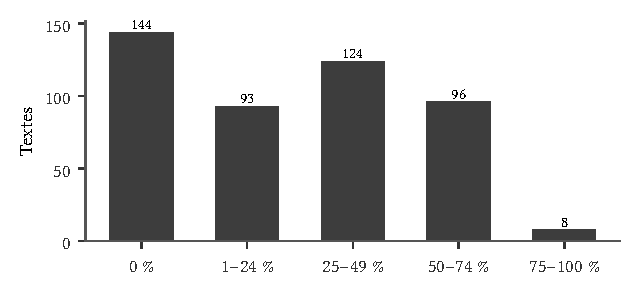
\includegraphics[width=0.8\linewidth]{figures/fig_restitution.pdf}
\caption{Part des lettres restituées par texte (ensemble C).}\label{fig:restitution}
\end{figure}

La figure~\ref{fig:restitution} donne la distribution de la part des lettres restituées. \st{nZeroRest} textes de l’ensemble C ne comportent aucune lettre restituée ; \st{nPlusMoitie} en ont plus de la moitié. Cette distribution rappelle qu’une grande partie du corpus est fragmentaire, et que toute mesure fondée sur le texte « avec restitutions » mesure, pour une part, le travail des éditeurs.

\chapter{Synthèse des résultats}\label{ch:synthese}

\section{Un corpus défini et contrôlé}

Le catalogue conserve les \st{nA} notices de la version précédente, avec leur numérotation. La confrontation des témoins a conduit à reconnaître trois paires de notices qui transmettent le même monument, un fragment à joindre à une autre notice et un texte extérieur à la période. Les analyses portent sur \st{nB} textes (ensemble B), dont \st{nC} textes funéraires (ensemble C) ; les deux dépositions successives d’une même plaque (\nnums{313} et 314) forment un seul monument, ce qui donne \st{nD} unités matérielles (chapitre~\ref{ch:corpus}).

Le texte de chaque notice est désormais confronté à un second témoin indépendant de l’EDCS. L’EDB a été appariée à \st{edbApp} notices ; pour \st{edbConc} d’entre elles, auxquelles s’ajoutent \st{edbConcRel} cas après relecture de la fiche détaillée, les deux lectures concordent ; pour \st{edbExam}, elles présentent des écarts mineurs ; pour \st{edbDiv}, une divergence forte ou un appariement douteux impose le retour à l’édition imprimée (chapitre~\ref{ch:transmission}). La seconde base apporte en outre ce que la première ignorait : le support, ses dimensions, la technique d’exécution, les signes figurés, le rattachement topographique, le lieu de conservation et les reproductions disponibles.

\section{Des années rapportées à leur fondement}

Chaque année de classement est rapportée à ce qui la fonde (chapitre~\ref{ch:fondement}). Dans l’ensemble C, l’année de \st{datLu} textes repose sur un nom consulaire lu, celle de \st{datPartiel} sur une lecture partielle, celle de \st{datInit} sur des initiales et celle de \st{datRest} sur un consulat restitué. Huit formules de date ne sont transmises que par l’EDB ; quatre années reposent sur une restitution conjecturale, quatre sur la seule base. Dix datations sont contestées, cinq font l’objet d’une réserve. Aucune année n’a été modifiée par vraisemblance ; les sept corrections apportées à l’année de la base reposent sur le texte.

Les contrôles calendaires éprouvent la cohérence des dates du jour : sur dix-huit mentions du jour de la semaine, dix concordent avec le calcul julien (dont une si l’on retient l’année 398 pour le \nnum{428}), cinq présentent un écart d’un jour qui reste inexpliqué, une est discordante et deux ne sont pas vérifiables ; et les deux mentions de l’âge de la lune sont compatibles avec les années proposées (chapitre~\ref{ch:calendrier}).

\section{Le formulaire, les signes et la langue}

La formule \emph{in pace} figure dans \st{ip_tot} textes funéraires (\st{ip_pct}~\%), dont près d’un quart seulement par restitution. Le noyau du formulaire (\emph{vixit}, \emph{depositus}, \emph{in pace}) est stable sur toute la période ; son recul apparent dans les textes tardifs tient en partie à leur état de conservation. Deux évolutions résistent mieux à ce biais : le recul des termes conjugaux et l’apparition, dans les dernières décennies, de \emph{plus minus}, des mentions d’emplacement et des actes d’achat (chapitre~\ref{ch:formulaire}).

Le chrisme et la croix sont décrits sur \st{nSignesC} textes funéraires, soit \st{pSignesC}~\% des textes appariés. Leur part paraît décroître au cours de la période ; ils sont plus fréquents sur les textes qui portent \emph{in pace} (chapitre~\ref{ch:supports}). La langue des épitaphes présente les traits graphiques du latin tardif ; l’accusatif de durée et l’ablatif coexistent, et la plupart des formes développées relèvent de l’éditeur (chapitre~\ref{ch:langue}).

\section{Les personnes}

L’ensemble C nomme \st{nPersAge} personnes dont l’âge est indiqué, après dix corrections de la table des personnes. L’âge médian est de \st{ageMed} ans ; l’attraction des âges ronds est forte (indice de Whipple : \st{whipple}), et l’expression \emph{plus minus} reconnaît l’approximation. Les épitaphes documentent le couple, la commémoration des enfants, le clergé marié et les lecteurs des titres, quelques clarissimes et quelques étrangers ; elles ne donnent pas une image de la population chrétienne de Rome (chapitres~\ref{ch:personnes} à \ref{ch:relations}).

\section{Le vocabulaire religieux}

Le langage doctrinal est rare. Selon la règle adoptée, \st{nProfilLarge}, \st{nProfilRestr} ou \st{nProfilStrict} textes désignent Dieu, le Christ, l’Esprit ou la Trinité par un mot lu ou abrégé (2,8, 2,4 ou 1,7~\%) ; \st{nProfilAvecRest} avec les restitutions. La Trinité est mentionnée une fois (\nnum{474}), l’Esprit saint au plus une fois et sur restitution (\nnum{249}), la résurrection jamais de manière assurée. Une seule demande d’intercession est assurée (\nnum{214}). L’identité chrétienne s’exprime surtout par le repos et la paix, par les signes, et par la qualification des personnes : sept néophytes, un catéchumène, des \emph{fideles}, des \emph{ancillae dei}, des vierges (chapitres~\ref{ch:typologie} à \ref{ch:textes_decisifs}).

\section{Les sépultures}

Quatorze textes enregistrent l’acquisition d’un emplacement, tous postérieurs à 369. Les vendeurs nommés sont des \emph{fossores} ; l’intervention du clergé n’est attestée que par des restitutions. La sépulture près des saints est présentée comme un privilège rare (\nnum{232}) (chapitre~\ref{ch:sepultures}).

\chapter{Discussion et conditions d’interprétation}\label{ch:discussion}

\section{Un corpus daté ne résout pas à lui seul la chronologie}

Les inscriptions datées sont utiles pour comparer des formes et des usages, à condition que l’événement daté et le texte observé appartiennent à une même phase documentable. Un document qui associe une naissance et une déposition n’offre pas deux années également pertinentes pour dater son formulaire ; une plaque préparée du vivant peut avoir reçu une addition ; une dalle qui commémore plusieurs défunts porte plusieurs dates (chapitre~\ref{ch:evenements}). Le retour aux éditions et au support conditionne l’emploi des dates comme jalons stylistiques.

La table des fastes utilisée pour identifier les consuls n’a pas été collationnée sur les \emph{Consuls of the Later Roman Empire} : elle suit la tradition des fastes telle qu’elle est reçue dans les bases, et l’EDB, qui cite cet instrument, a servi de contrôle indirect. Les divergences d’itération, de collègue et de post-consulat restent ouvertes lorsqu’aucun témoin contrôlé ne permet de choisir. La vraisemblance d’une correction ne vaut pas preuve de la leçon.

\section{Deux bases ne font pas une édition}

La confrontation de l’EDCS et de l’EDB a été le principal instrument de cette révision. Elle a permis de récupérer des formules de date, des lignes omises, des parties grecques et des données matérielles ; elle a révélé des erreurs de saisie et des restitutions divergentes. Mais deux bases qui concordent ne garantissent pas une lecture : elles suivent souvent la même édition, et leurs accords peuvent reproduire la même erreur. Les « lectures stabilisées » de ce volume sont des lectures concordantes entre deux témoins secondaires ; elles ne sont pas des lectures collationnées sur les ICVR ni sur les monuments. Un export est un état de transmission, non un substitut transparent à l’édition.

\section{Le formulaire n’est pas une confession de foi exhaustive}

La présence d’une formule de paix ou de repos renseigne sur un choix de commémoration ; elle ne fournit pas une échelle d’adhésion doctrinale. L’absence d’une énumération du Père, du Fils et de l’Esprit dans \emph{ancilla dei et Chr(isti)} ne contredit pas une croyance trinitaire ; la présence de \emph{trinitatem} au \nnum{474} n’autorise pas à reconstruire des lignes perdues qui nommeraient les trois personnes.

L’énoncé fragmentaire et le genre du texte sont deux contraintes distinctes. Un texte bref a moins d’espace pour développer une doctrine ; un texte lacunaire peut avoir perdu ce qui la formulait. Sans série comparative définie et sans contrôle des longueurs et des pertes, le corpus ne permet pas de répartir les causes de la rareté du langage doctrinal (chapitre~\ref{ch:rarete}).

Le signe figuré pose un problème de même nature. Le chrisme, présent sur un texte sur sept parmi ceux que l’EDB décrit, dit l’appartenance chrétienne du monument plus souvent que les mots. Sa description dépend toutefois des rédacteurs de la base, et sa fonction — compendium du nom, signe juxtaposé, ornement — ne peut être établie que sur la pierre ou sur une photographie.

\section{Familles, opérateurs et institutions}

Les achats d’emplacements auprès de fossoyeurs attestent des opérations et des acteurs nommés. Ils ne suffisent pas à établir la propriété juridique des cimetières ni le degré de centralisation de leur gestion. La mention d’un évêque n’en fait pas automatiquement le vendeur : le datif \emph{Pascasio ep(is)c(opo)} du \nnum{400} appelle une analyse de relation et de fonction. La restitution \emph{a presbyteris} du \nnum{387} ne peut être mise sur le même plan qu’un nom de fonction lu. De même, la proximité recherchée des saints, telle que le \nnum{232} la donne à lire, ne mesure pas la distribution sociale des emplacements. Ces dossiers peuvent être confrontés aux problématiques de Charles Pietri, d’Éric Rebillard et de Steffen Diefenbach ; les développements de ces ouvrages qui ne sont connus ici que par leurs notices ou par des comptes rendus ne sont pas invoqués comme arbitres d’une décision.

\section{Les données numériques comme témoins}

La lecture méthodologique de Heřmánková, Kaše et Sobotková invite à distinguer le classement religieux de la fonction sociale, et la précision apparente d’une donnée de sa résolution réelle\footnote{P.~Heřmánková, V.~Kaše, A.~Sobotková, « Inscriptions as Data: Digital Epigraphy in Macro-historical Perspective », \emph{Journal of Digital History}, 1/1, 2021, DOI 10.1515/jdh-2021-1004.}. Dans ce volume, cette exigence se traduit par trois règles : ne pas confondre fiches et monuments ; ne pas confondre coordonnées bibliographiques et contexte archéologique ; ne pas confondre proportions documentaires et fréquences de population.

\section{Ce qui reste à faire}

Trois chantiers conditionnent l’exploitation historique de ce corpus au-delà de ce que le présent volume établit.

\begin{enumerate}
\item \emph{La collation des éditions.} Les textes à divergence forte (\st{edbDiv}), les seize textes absents de l’EDB et les formules de date contestées doivent être collationnés sur les ICVR et, pour les textes antérieurs, sur les éditions de De Rossi et de Diehl.
\item \emph{Le contrôle photographique.} Les reproductions signalées par l’EDB (\st{nFacsim} textes) permettraient de trancher la question des monogrammes, de vérifier les lettres soulignées par l’EDB et de contrôler les restitutions des textes décisifs (chapitre~\ref{ch:textes_decisifs}).
\item \emph{La collation des fastes.} La table consulaire doit être confrontée à la CLRE pour les années contestées.
\end{enumerate}

Ces conditions ne sont pas un ajout périphérique au livre. Elles déterminent les propositions que le lecteur peut tenir pour établies, celles qu’il peut tester à partir des données publiées, et celles qui restent à instruire.

\chapter{Conclusions}\label{ch:conclusions}

Ce corpus fournit une documentation située sur les manières de nommer les morts, de dater des événements et de représenter les relations dans les inscriptions chrétiennes de Rome entre 340 et 403. Il ne suffit ni à reconstituer la population chrétienne de la Ville, ni à mesurer l’adhésion doctrinale des commanditaires. Sa valeur tient à la possibilité de relier chaque proposition au texte transmis, à son second témoin et à son statut documentaire.

La confrontation systématique de deux bases épigraphiques indépendantes a transformé l’état du dossier. Elle a fait apparaître des formules de date que le premier témoin omettait (\nnums{84}, 214, 268, 388, 447…), des lignes absentes de l’un ou de l’autre (\nnums{306}, 378), des restitutions divergentes qui commandent l’interprétation (\nnums{73}, 447), des erreurs de saisie (dates de l’EDB aux \nnums{206} et 278 ; table des personnes de la base de travail), et des données matérielles jusque-là ignorées : supports, dimensions, signes, reproductions. Elle a aussi montré ses limites : deux bases qui concordent ne font pas une édition collationnée.

La chronologie a été rapportée à ses fondements. Naître, mourir, être déposé, acquérir une tombe et faire graver un texte ne sont pas une même opération. Une concordance arithmétique contrôle une relation, non l’ensemble d’une lecture ; une discordance appelle l’examen du témoin et n’autorise pas à normaliser silencieusement le texte. L’année de classement de chaque notice est conservée ; sa solidité est qualifiée.

Le vocabulaire religieux appelle la même discipline. Les désignations de Dieu et du Christ sont rares, la Trinité n’est mentionnée qu’une fois, l’Esprit saint au plus une fois et sur restitution, la résurrection jamais de manière assurée. La foi s’exprime surtout par la paix et le repos, par le chrisme, et par la qualification des personnes — \emph{fidelis}, \emph{neophytus}, \emph{ancilla dei}, \emph{virgo}. Quelques poèmes, souvent issus de milieux aisés ou proches du clergé, développent l’espérance d’une vie éternelle, de la lumière et de la société des saints. Le silence doctrinal du genre ne peut être lu comme le silence d’une communauté.

La contribution du volume est ainsi documentaire et méthodologique avant d’être interprétative : distinguer les niveaux de transmission, publier les règles de compte, confronter les témoins, conserver les états antérieurs et limiter chaque inférence à la résolution des preuves disponibles. Le catalogue, les données et les programmes qui produisent chaque tableau sont publiés avec le livre, afin que toute mesure puisse être recalculée et toute décision contestée. L’établissement philologique complet, qui suppose la collation des éditions imprimées et des monuments, reste une étape distincte ; ce volume en fournit l’instrument et en délimite le programme.


\part{Dossiers commentés et catalogue raisonné}
\chapter{Dossiers commentés}\label{ch:dossiers}

Ce chapitre réunit des dossiers sur quarante-sept textes du corpus, choisis pour leur intérêt philologique, chronologique ou historique, et en particulier tous les textes dont dépendent les conclusions des chapitres précédents. Chaque dossier donne, après une ligne de données (année de classement et fondement, références, rattachement topographique, support selon l’EDB, renvoi à la notice du catalogue), le texte transmis par l’EDCS, ligne à ligne, puis le texte de l’EDB lorsqu’il existe. Les deux témoins sont reproduits sans harmonisation : leurs différences de notation (⸢ ⸣ et \emph{(!)} pour l’EDCS ; ⟨ ⟩, ⌜ ⌝, lettres soulignées ou pointées et descriptions de signes entre doubles parenthèses pour l’EDB) sont celles des bases (chapitre~\ref{ch:edition}). Viennent ensuite une traduction et un commentaire.

Les traductions sont littérales ; les crochets y signalent les passages qui traduisent une restitution. Elles ne remplacent pas une traduction établie sur l’édition imprimée. Aucun des textes n’a été collationné sur la pierre ou sur une photographie, à l’exception partielle du \nnum{38}.

\dossier{4}{Iunianus et Victora, « amis des pauvres »}
\trad{Déposition de Iunianus, la veille des ides d’avril (12 avril), sous le consulat de Marcellinus et de Probinus. Il vécut quarante ans et mourut en paix ; ami des pauvres, il vécut avec sa \emph{virginia} quinze ans. À lui, bien méritant, sa \emph{virginia} Victora (\emph{Bictora}), bien méritante, a fait (ce monument) : amie des pauvres et travailleuse.}
\comm{La plus ancienne épitaphe du corpus qui emploie \emph{virginia} pour l’épouse épousée vierge (chapitre~\ref{ch:personnes}). Les deux époux reçoivent la même qualification d’« amis des pauvres » (\emph{amator}, \emph{amatrix pauperum}, avec la graphie \emph{paupe\{ro\}rum} que l’EDCS corrige et que l’EDB conserve) ; l’épouse est en outre \emph{operaria}, mot qui peut désigner une travailleuse manuelle ou, dans un sens plus particulier, une personne active dans les œuvres charitables, ce que le texte ne permet pas de préciser. Le bêtacisme est constant (\emph{bixit}, \emph{birginia}, \emph{Bictora}). L’EDB décrit un monogramme du Christ à la fin du texte, que l’EDCS ne signale pas. La date de 341 repose sur une formule consulaire lue en entier.}

\dossier{15}{Cassia, \emph{clarissima femina}}
\trad{[…] Cassia, (fille ou épouse) de Piso, \emph{clarissima femina}, vécut trente ans et quatre-vingt-treize jours ; née sous le consulat de Sabinus et Rufinus, le dix-septième jour avant les calendes de juillet (15 juin 316), elle rendit (l’âme) après le consulat d’Amantius et d’Albinus, le dix-septième (EDB : seizième) jour avant les calendes d’octobre (15 ou 16 septembre 346).}
\comm{Le génitif \emph{Pisonis} peut désigner le père ou le mari. Le texte est gravé sur un sarcophage (17 × 130 cm selon l’EDB, qui donne sans doute les dimensions du seul champ inscrit). Il contient deux dates consulaires, celle de la naissance (316) et celle de la mort (post-consulat de 345, soit 346) ; l’année de classement est celle de la mort. La durée de vie gravée, trente ans et quatre-vingt-treize jours, concorde avec les deux dates, selon le mode de décompte (chapitre~\ref{ch:calendrier}) : du 15 juin au 15 septembre, on compte quatre-vingt-treize jours en décompte inclusif, et autant jusqu’au 16 septembre en décompte exclusif. Les deux bases divergent sur le quantième du décès (XVII ou XVI), et l’EDB restitue le nom du mois ; la concordance arithmétique ne permet pas de choisir entre les deux lectures. Le verbe \emph{reddit}, employé absolument, appartient au vocabulaire de la mort comme restitution (de l’âme ou de la vie).}

\dossier{22}{Caianus, juriste}
\trad{(Vers) Heureuse fut la vie de cet homme, plus heureux encore son trépas : le nom de Caianus croît sans cesse au fil des siècles ; la renommée ne sait pas mourir, mais vit toujours et partout. Hôte romain, il vint dans la ville du prince ; il fut ici d’abord jurisconsulte et ami. — Il repose en paix ; déposé le quatrième jour avant les nones d’août (2 août), sous le consulat de Flavius Philippus et de Flavius Salia (348). Son père Sabbatius a fait (ce monument).}
\comm{Épitaphe métrique (CLE 659) d’un jurisconsulte. Les quatre hexamètres reprennent les lieux communs de la gloire posthume (\emph{nescit fama mori}) ; la partie en prose emploie le formulaire chrétien (\emph{quiescit in pace}, avec la graphie \emph{pacem}). Le vers \emph{advenit hospes Romanus princeps in urbem} est obscur : \emph{princeps} peut qualifier la ville (« la ville capitale ») ou désigner le prince ; la traduction proposée reste incertaine. L’EDB décrit un oiseau et un chrisme radié. Le père porte un nom dérivé du sabbat, \emph{Sabbatius} (chapitre~\ref{ch:noms}).}

\dossier{26}{Esuvia Ianuaria et Aradius Melissus}
\trad{D’une bonté et d’une sainteté admirables : à Esuvia Ianuaria, son épouse, qui vécut avec moi dix-huit ans, cinq mois et vingt-cinq jours, Aradius Melissus, son mari, a fait (ce monument), et pour lui-même ; déposée en paix le troisième jour avant les calendes d’avril (30 mars), sous le consulat de Philippus et de Salia (348).}
\comm{Le texte ne donne pas l’âge de la défunte, mais la durée de la vie commune (\emph{vixit mecum}), avec la même précision qu’un âge ; la table des personnes ne lui attribue donc pas d’âge (chapitre~\ref{ch:personnes}). Le mari prépare sa propre sépulture (\emph{et sibi fecit}). Le texte n’est pas apparié à l’EDB ; il est connu par l’ICVR II 5711 et par une publication de 2012.}

\dossier{36}{Clodius Adelfius, ancien préfet de la Ville}
\trad{Clodius Adelfius, \emph{vir clarissimus}, ancien préfet de la Ville, à son épouse incomparable et pour lui-même a fait (ce monument).}
\comm{Le texte est gravé en colonne étroite, une ou deux syllabes par ligne, disposition que les deux bases reproduisent. Il ne contient aucune date : l’année 351 de la base dépend de l’identification de Clodius Adelfius à Clodius Celsinus Adelphius, préfet de la Ville en 351, et marque un terme postérieur, non l’année du décès (chapitre~\ref{ch:fondement}). La bibliographie fait de ce préfet l’époux de la poétesse chrétienne Faltonia Betitia Proba ; l’identification et cette relation sont à contrôler dans la \emph{Prosopography of the Later Roman Empire}. Le texte, sans formule chrétienne, est classé dans le corpus en raison de sa publication parmi les inscriptions chrétiennes (ICVR I 19).}

\dossier{38}{Privata, \emph{in pace} et le monogramme}
\trad{Privata, qui vécut cinquante-trois ans, huit mois et deux jours, a été déposée le quatrième jour avant les nones de février (2 février) ; bien méritante, en paix ☧ ; sous le consulat de Decentius et de Paulus (352).}
\comm{Dossier de référence pour la question du monogramme (chapitre~\ref{ch:dieu_christ}). L’EDCS développe \emph{Chr(isti)} ; l’EDB transcrit \emph{((monogramma Christi))} ; l’estampage conservé à l’Ohio State University sous le numéro ILCV 3252A montre un christogramme placé après IN PACE. La pierre porte donc un signe, non le mot écrit en lettres. La traduction rend le signe par ☧ sans décider s’il se lit \emph{Christi} (« dans la paix du Christ ») ou s’il est juxtaposé à la formule. Le texte provient, selon l’EDB, du cimetière à ciel ouvert proche de la basilique Saint-Pierre ; il est conservé au Lapidario Cristiano des Musées du Vatican. La forme \emph{meses} pour \emph{menses} est signalée par les deux bases.}

\dossier{43}{Anastasius, poème de Constantia}
\trad{(Vers) Au nom [du Christ …]. Affligée, [Constantia écrit ces vers] pour Anastasius, son époux, qui [a échangé] la lumière [contre d’amères ténèbres] ; sa vie [s’arrêta] à quatre fois dix [et cinq ans] ; combien vite il fut ravi [à l’amour de son épouse chérie] ! Pleuré [quand Janus prenait] son douzième [lever], il fut enseveli [l’année que conduisait] le consul Arbitio (355).}
\comm{Les deux bases donnent la même restitution, empruntée à l’édition : chaque vers est conservé sur sa moitié gauche, et la seconde moitié est reconstituée selon le mètre et le sens. Le nom du Christ, dans l’invocation initiale, est entièrement restitué ; l’EDB décrit un chrisme avec alpha et oméga, qui rend l’invocation vraisemblable sans la rendre lisible. L’année repose sur le nom d’Arbitio, lu (\emph{Arbitio co[nsul]}) ; la date du jour (\emph{duodecimum [Ianus]}) est une restitution. L’âge, « quatre fois dix [et cinq] », est en partie restitué.}

\dossier{70}{Secunda, \emph{virgo fidelis}}
\trad{À Secunda, d’une bonté admirable, qui vécut d’une foi pure vingt ans ; chaste, elle a cessé (de vivre) en paix, vierge fidèle ; bien méritante, elle repose ; aux ides de juillet (15 juillet) ; colombe sans fiel ; sous (le consulat de) M(amertinus) et N(evitta) (362).}
\comm{L’un des deux seuls textes datés par les seules initiales des consuls (chapitre~\ref{ch:fondement}) ; l’identification de l’année 362 repose sur le couple M. et N., que seul le collège de Mamertinus et Nevitta satisfait dans la période. Le vocabulaire est celui de la virginité consacrée probable (\emph{pura fide}, \emph{pudica}, \emph{virgo fidelis}) ; l’image de la colombe sans fiel (\emph{palumbo sine felle}, au masculin) appartient au langage chrétien de l’innocence. L’EDB lit \emph{quiescet} et conserve \emph{\{id\}}, que l’EDCS considère également comme superflu.}

\dossier{72}{Flavia Balbilla : \emph{Dis Manibus} et \emph{in pace}}
\trad{Consacré aux dieux Mânes. Flavia Balbilla vécut vingt-huit ans, six mois et douze jours ; elle a reposé en paix sous le consulat de Mamertinus et de Nevitta, Maximus étant préfet de la Ville, le cinquième jour avant les calendes de février (28 janvier 362).}
\comm{Seul texte de l’ensemble C qui porte la dédicace aux Mânes, associée au verbe chrétien du repos (\emph{requievit in pace}). Les deux formules coexistent sans difficulté apparente pour le commanditaire ; la dédicace \emph{D. M. s.} est alors une formule d’ouverture traditionnelle plus qu’une profession religieuse. Le texte est aussi le seul du corpus à dater par le préfet de la Ville en plus des consuls (chapitre~\ref{ch:rangs}). L’EDB transmet la graphie \emph{Nebidda}, que l’EDCS normalise.}

\dossier{73}{Eleuteria : l’esprit, les saints et les hauteurs}
\trad{(Vers) [Voici] la demeure éternelle où tu reposes désormais en sécurité ; […] ton esprit, se retirant de la chair, [vit avec / est associé aux] saints, pour tes mérites et tes si grandes œuvres ; [toi qui …] tu reposes toujours en sécurité ; [tu as confié ton corps] à la terre et le gage reçu ; […] à la splendeur avec une claire lumière ; […] toi qui t’es toujours consacrée à Dieu ; […] mais pour tes actions tu es appelée vers les hauteurs ; […] Pacatianus doit beaucoup […]. Pacatianus a fait cet emplacement pour Eleuteria, sa mère, qui vécut environ soixante-quinze ans, deux mois et dix jours ; déposée le quatrième jour avant les calendes de juin (29 mai) ; elle dort [en paix], sous le consulat de notre seigneur Claudius Iulianus Auguste pour la quatrième fois et de Flavius Sallustius (363). Hesperius, qu’elle a nourri, l’a gravé.}
\comm{Le poème est conservé sur sa partie droite, et les deux bases restituent différemment le début des vers (chapitre~\ref{ch:typologie}). La traduction ne retient que ce qui est commun : l’esprit se sépare de la chair (lu), il est en relation avec les saints (\emph{sanctis}, lu ; le verbe est restitué), la défunte s’est consacrée à Dieu (\emph{deo dica⟨vi⟩sti}, lu dans l’EDB, \emph{dicasti} dans l’EDCS) et elle est appelée « vers les hauteurs » (lu). Le séjour \emph{in caelo} et la crainte de Dieu (\emph{[deu]m metuisti}) ne sont que des restitutions de l’EDCS ; l’EDB lit \emph{[- - - de]metuisti}. Le texte nomme trois personnes : la défunte, son fils Pacatianus, qui fait l’emplacement, et Hesperius, son nourricier, qui grave. L’EDB décrit des palmes, un soleil, un chrisme, une croix gammée, un alpha et un oméga, disposés à la fin des vers.}

\dossier{110}{Benenatus, ancien \emph{comes}, et Theophila}
\trad{(Grec) En paix a reposé Benenatus, ancien \emph{comes}, ayant vécu soixante-quinze ans ; il gît en ce lieu, sorti de la vie le quatrième jour avant les ides de mars (12 mars), sous le consulat de Lupicinus et de Iovinus (367) ; moi, Theophila, j’ai fait (ce monument) pour mon époux. — (Latin) À Benenatus, Theophila, son épouse, a fait (ce monument).}
\comm{Épitaphe bilingue, dont le grec porte l’essentiel (chapitre~\ref{ch:grec}). Le formulaire grec (\emph{ἐν εἰρήνῃ ἀνεπάη}) est l’équivalent du \emph{requiescit in pace} latin ; la date romaine est transposée en grec. L’abréviation \emph{ἀπ(ὸ) κο(μήτων)} désigne un ancien \emph{comes}, sans préciser la fonction. Les graphies \emph{κῖτε} et \emph{ἐξελτών} reflètent la prononciation contemporaine. Le nom de l’épouse, \emph{Theophila}, est théophore.}

\dossier{118}{Ianuaria : l’âge à l’heure près}
\trad{Sous le consulat de Lupicinus et de Iovinus (367), Ianuaria, qui vécut vingt-quatre ans, un jour et deux heures et demie, s’en est allée un mardi.}
\comm{Seul texte du corpus qui donne, sans restitution, une durée de vie en heures (chapitre~\ref{ch:personnes}). L’EDB ne transcrit pas \emph{s(emis)} et lit \emph{XXI III}, ce qui pourrait signaler une disposition particulière des chiffres sur la pierre ; elle décrit l’image de la défunte et des colombes. Le quantième n’est pas donné : le mardi ne peut être contrôlé (chapitre~\ref{ch:calendrier}). Les deux noms consulaires sont gravés au datif ou à l’ablatif avec \emph{in consulatu}, construction que l’EDCS signale par \emph{(!)}.}

\dossier{126}{Un fils né en 350, mort en 368}
\trad{Ses parents affligés ont fait ce que lui-même aurait dû faire ; malheureux parents, (contraints) par la douleur à ce devoir, ils ont fait aussi ce tombeau. Il naquit sous le consulat de Flavius Sergius et de Flavius Nigrinianus (350), le troisième jour avant les ides d’août (11 août), un samedi ; il a été déposé dans cette demeure éternelle sous le consulat de nos seigneurs Valentinien et Valens, Augustes pour la deuxième fois (368), le septième jour avant les ides de décembre (7 décembre), un samedi ; il vécut dix-neuf ans, trois mois et vingt-six jours ; en paix.}
\comm{Le topos de l’inversion des devoirs (les parents font pour l’enfant ce que l’enfant aurait dû faire pour eux) ouvre le texte. Les deux dates sont complètes. Le calcul confirme le samedi de la naissance ; le 7 décembre 368 est un dimanche, soit un écart d’un jour avec le samedi gravé. Les mois et les jours de l’âge concordent exactement avec l’intervalle entre les deux dates, mais l’intervalle est de dix-huit ans et non de dix-neuf (chapitre~\ref{ch:calendrier}). La durée gravée, \emph{XVIIII}, est lue identiquement par les deux bases ; l’écart d’une année reste inexpliqué. La tombe est une \emph{domus aeterna}.}

\dossier{133}{Felix, « appelé à la sainte foi »}
\trad{Felix, appelé à la sainte foi, s’en est allé en paix ; un si grand amour et une si grande affection sont gardés pour lui par ses amis à jamais ; de son vivant, il fut un réconfort, miséricordieux, connu de tous. Agrippina a fait (ce monument) pour son très doux mari, avec qui elle vécut sans blessure de l’âme trois ans et dix mois ; il fut dans le siècle, tant qu’il vécut, trente-deux ans ; déposé le treizième jour avant les calendes de septembre (20 août), sous le consulat de Valentinien, très noble enfant, et de Victor (369).}
\comm{L’expression \emph{sanctae fidei vocitus} peut évoquer une conversion ou un baptême ; le texte ne précise pas lequel (chapitre~\ref{ch:foi_eglise}). La durée de la vie commune (trois ans et dix mois) avait été enregistrée comme un âge dans la table des personnes ; elle est corrigée (chapitre~\ref{ch:personnes}). L’éloge de Felix (\emph{solacius}, \emph{misericors}) relève de la charité ; l’expression \emph{fuit in saeculum} oppose la vie terrestre à ce qui suit. L’EDB rattache le texte à la basilique Saint-Pierre.}

\dossier{134}{Une dalle familiale : un prêtre, un diacre et leur sœur}
\trad{(a) Endormissement de Dulcitius, prêtre, aux calendes de février (1\textsuperscript{er} février), et de Gregorius, diacre, le treizième jour avant les calendes de mai (19 avril), et de Catafronia (EDB : Califronia), leur sœur, le cinquième jour avant les ides de mars (11 mars). (b) Déposition de Faustina le quatrième jour avant les calendes de novembre (29 octobre), sous le consulat de Valentinien, très noble enfant, et de Victor (369). (c) Endormissement d’Agapè le quatrième jour avant les nones (EDB : aux nones) d’octobre, en paix.}
\comm{La grande dalle (105 × 190 × 15 cm selon l’EDB), retrouvée en morceaux remployés dans un mur de la basilique des Saints-Nérée-et-Achillée, porte trois textes distincts, que l’EDB distingue (a, b, c). Seule la partie b est datée : l’année de classement ne vaut pas pour les autres défunts (chapitre~\ref{ch:evenements}). Le texte atteste une famille cléricale (un prêtre, un diacre et leur sœur) et l’emploi de \emph{dormitio} pour désigner la mort. Les deux bases divergent sur le nom de la sœur et sur la date d’Agapè.}

\dossier{140}{Bonifatia, \emph{in pace Chr(isti)}}
\trad{À Bonifatia, bien méritante, dans la paix du Christ, qui vécut vingt-huit ans ; déposée en paix le douzième jour avant les calendes de septembre (21 août), sous le consulat de Valentinien et de Valens pour la troisième fois (370).}
\comm{La formule \emph{in pace Chr(isti)} suit \emph{bene merenti} et précède une seconde mention de la paix (\emph{deposita in pace}). Les deux bases transcrivent une abréviation, mais l’EDB décrit un chrisme parmi les données matérielles : il est probable que l’abréviation développée rende un monogramme employé comme compendium (chapitre~\ref{ch:dieu_christ}). L’EDB rattache le texte au cimetière de Pontien.}

\dossier{151}{Muscula, dite aussi Galatea}
\trad{Ici gît Muscula, dite aussi Galatea, qui vécut deux ans, deux mois et dix-sept jours ; déposée le quinzième jour avant les calendes d’août (18 juillet), sous le consulat de Gratien Auguste pour la deuxième fois et de Probus (371), dans la paix du Christ.}
\comm{La formule \emph{in pace Chr(isti)} occupe une place inhabituelle : elle clôt le texte, après la date consulaire. Comme au \nnum{140}, les deux bases transcrivent une abréviation et l’EDB décrit un chrisme sur le support (chapitre~\ref{ch:dieu_christ}). Le double nom (\emph{quae et}) n’a pas de portée religieuse. Le texte provient, selon l’EDB, du cimetière de Commodilla ; il est conservé au Lapidario Cristiano.}

\dossier{183}{Petronia, vierge, de la neuvième région}
\trad{Déposition de Petronia le sixième jour avant les calendes de décembre (26 novembre), après le consulat de Gratien Auguste pour la troisième fois et de Flavius Equitius (375) ; elle vécut vierge environ dix-neuf ans ; elle est en paix ; (elle était) de la neuvième région, du côté du lac du \emph{Cuniculus}.}
\comm{Le mot \emph{virgo} peut désigner une jeune fille non mariée ou une vierge consacrée ; rien dans le texte ne permet de choisir (chapitre~\ref{ch:foi_eglise}). L’indication de domicile dans la neuvième région augustéenne, \emph{a lacu cuniculi}, est exceptionnelle dans le corpus ; la localisation de ce repère relève de la topographie de Rome et n’est pas proposée ici. L’EDB rattache le texte au cimetière de Zénon et décrit un chrisme, un paon et un rameau d’olivier ; la plaque est conservée au Collegio Teutonico.}

\dossier{202}{Cinnamius Opas, lecteur du titre de Fasciola}
\trad{Cinnamius Opas, lecteur du titre de Fasciola, ami des pauvres, qui vécut quarante-six ans, sept mois et neuf jours ; déposé en paix le dixième jour avant les calendes de mars (20 février), sous le consulat de Gratien pour la quatrième fois et de Merobaudes (377).}
\comm{L’un des trois lecteurs rattachés à un titre de la Ville (chapitre~\ref{ch:rangs}). Le \emph{titulus Fasciolae} est de nouveau nommé au \nnum{421} (398), avec le lecteur Pascentius. L’âge du défunt montre que la fonction de lecteur pouvait être exercée à l’âge mûr. La qualification \emph{amicus pauperum} associe le clerc à l’assistance. Le texte n’est pas apparié à l’EDB.}

\dossier{209}{Victorinus achète son emplacement au fossoyeur Martinianus}
\trad{Cet emplacement est celui de Victorinus, qui l’a acheté au fossoyeur Martinianus, sous (le consulat de) Valens pour la sixième fois et de Valentinien (pour la deuxième fois) (378).}
\comm{Le plus ancien acte d’achat daté du corpus qui nomme le vendeur, un \emph{fossor} (chapitre~\ref{ch:sepultures}). L’acte, sans commémoration, n’entre pas dans l’ensemble C. L’EDB restitue l’itération du second consul (\emph{Valentin[iano bis]}) et décrit, en tête du texte, un monogramme du Christ avec alpha et oméga : le signe chrétien marque ici un document de propriété.}

\dossier{214}{\emph{Ancilla dei} : « prie pour ce seul enfant »}
\trad{Ici repose une servante de Dieu, qui de ses biens a possédé tout entière cette demeure, que ses amies pleurent et dont elles cherchent le réconfort. Prie pour ce seul (enfant), la descendance que tu as laissée survivante. — (EDB seule :) Tu demeureras dans le repos éternel de la félicité ; le [quantième anomal] jour avant les calendes d’octobre. Cucurbitinus et Abundantius reposent ici ensemble. Sous le consulat de nos seigneurs Gratien pour la cinquième fois et Théodose, Augustes (380).}
\comm{Le seul témoignage assuré du corpus d’une demande d’intercession adressée au défunt (chapitre~\ref{ch:mort_esperance}). La défunte, \emph{ancilla dei}, est priée d’intercéder pour l’enfant qui lui survit. L’expression \emph{de sua omnia possedit domum ista} indique qu’elle a acquis la tombe sur ses propres biens. L’EDCS s’arrête à \emph{reliquisti} ; l’EDB transmet trois lignes supplémentaires, qui donnent la date et nomment deux autres défunts inhumés dans la même tombe. L’année 380 repose sur ces lignes. La plaque (69 × 128 cm) est conservée à la villa Albani ; l’EDB décrit des oiseaux tenant une couronne.}

\dossier{231}{Celerinus, enfant \emph{fidelis}}
\trad{Innocent, il s’en est allé, (enfant) des innocents, miséricordieux il fut. Qui n’a pas souffert de ton âge et versé de pieuses larmes ? En toi était attendue l’espérance de l’avenir, par toi une gloire durable, Celerinus, mon fils. Fidèle, tu reposes en paix. Il vécut un an et quatre mois ; déposé le sixième jour avant les calendes d’octobre (26 septembre), sous (le consulat d’)Antonius et de Syagrius (382).}
\comm{L’application de \emph{fidelis} à un enfant de seize mois suggère qu’il était baptisé (chapitre~\ref{ch:foi_eglise}). Le texte développe une rhétorique de la perte : l’enfant portait l’espérance et la gloire de la famille. L’EDB lit \emph{d(iebus) VI} là où l’EDCS lit \emph{d(epositus) VI} : la seconde lecture fait de \emph{VI Kal. Oct.} la date de la déposition, la première l’intègre à l’âge. La traduction suit l’EDCS.}

\dossier{232}{\emph{Intra limina sanctorum} : une sépulture recherchée}
\trad{[…]na, servante dans le Seigneur (?), […] a nourri […] les siens ; [amie des] pauvres ; [qui pour de si grands] mérites a reçu [une sépulture à l’intérieur des] seuils des saints ; […] a reçu [ce que beaucoup désir]ent et que peu obtiennent ; [sous le consulat d’Antonius et de] Syagrius (382).}
\comm{Le texte est conservé sur sa partie droite. Trois éléments intéressent l’histoire religieuse (chapitres~\ref{ch:mort_esperance} et~\ref{ch:sepultures}). (1) \emph{in dom(ino?) cultrix} : l’abréviation est développée avec un point d’interrogation par l’éditeur ; le texte n’est retenu que dans le profil large. (2) \emph{[- - - l]imina sanctorum} : la fin de l’expression est lue ; le mot qui la précédait est restitué. (3) \emph{[- - -]n(t) et rari accipiun(t)} : la seconde moitié de l’antithèse est lue. Le texte présente la sépulture près des saints comme la récompense des mérites d’une femme charitable et comme un privilège rare. Il ne dit pas quels saints, ni où ; il est d’origine incertaine.}

\dossier{244}{Proiecta : une épigramme de Damase}
\trad{(Vers) Que dire ? Ou me taire ? La douleur même m’interdit de parler. Ce tombeau retient les larmes — sache-le — des parents de Proiecta, qui avait été unie à Primus, son mari, belle de sa grâce, contente de sa seule pudeur. Hélas, trop chérie de l’amour d’une mère malheureuse ! Apprends ce qu’elle eut de plus que bien d’autres : après les premiers liens du mariage, arrachée aux yeux de Florus, son père, elle s’en est allée, désirant monter vers la lumière éthérée du ciel. Ces consolations des pleurs, Damase les offre à tous. — Elle vécut seize ans, [dix mois] et vingt-cinq jours ; déposée le troisième jour avant les calendes de janvier (30 décembre), sous le consulat de Flavius Merobaudes et de Flavius Saturninus (383).}
\comm{L’épigramme est signée par l’évêque de Rome Damase (366–384), et la formule consulaire la date de la dernière année de son épiscopat. Elle figure dans l’édition commentée de Trout (\emph{Damasus of Rome. The Epigraphic Poetry}, 2015, n\textsuperscript{o}~51 selon la concordance de l’EDCS) et dans les \emph{Carmina Latina Epigraphica} (CLE 670). Le texte ne nomme ni le Christ ni Dieu ; l’espérance de la défunte est exprimée dans le langage de l’ascension céleste. Le rapprochement avec la Proiecta nommée sur le coffret du trésor de l’Esquilin a été discuté dans la bibliographie consacrée à ce trésor ; il n’est pas repris ici. Les mots \emph{m(enses) X} sont signalés par l’EDCS comme une addition (\emph{«  »}).}

\dossier{249}{« Qui a reçu l’Esprit saint »}
\trad{[…] qui a reçu l’[Esprit] saint, [le seizième jour avant les calendes] de mai (16 avril ?), sous le consulat de Merobaudes [pour la deuxième fois] (383).}
\comm{Dossier examiné au chapitre~\ref{ch:esprit_trinite}. Sont lus \emph{-tus est qui ac-}, \emph{-tum spiritum}, \emph{Mai(as) Merobaud-}. Le verbe (\emph{ac[cepti]} dans l’EDCS, \emph{ac[cepit]} dans l’EDB), le début de l’adjectif, le quantième et l’itération du consulat sont restitués. La mention de l’Esprit saint est probable ; le rite qu’elle désigne et sa date ne peuvent être précisés. Le fragment (20 × 23,5 cm) provient, selon l’EDB, du cimetière de Nicomède, sur la via Nomentana.}

\dossier{268}{Lucifer, par son fils Benedictus}
\trad{Ce tombeau de son père, son fils Benedictus a voulu qu’il fût fait, par amour et en souvenir de son père, pour Lucifer, homme très innocent, [ami] des amis, qui, tant qu’il fut dans les choses humaines, parut très disponible envers tous et doux ; car il vécut toujours sans [faute de son] temps soixante-cinq ans, six mois et douze jours ; il mourut [en paix (?)]. — (EDB seule :) Le septième jour avant les calendes de juillet (25 juin), sous le consulat de Richomeres et de Clearchus (384).}
\comm{L’EDCS s’arrête à \emph{decess[it]} ; l’EDB transmet la dernière ligne, qui donne la date et fonde l’année 384 (chapitre~\ref{ch:fondement}). L’EDB souligne de nombreuses lettres, lues par les éditeurs anciens et aujourd’hui perdues. Le nom du défunt, \emph{Lucifer}, et celui du fils, \emph{Benedictus}, appartiennent l’un à l’onomastique traditionnelle, l’autre à l’onomastique chrétienne (chapitre~\ref{ch:noms}). La plaque (64 × 98 cm) est conservée à la Galleria Lapidaria des Musées du Vatican.}

\dossier{275}{Quirillus, Arménien de Cappadoce}
\trad{Citoyen arménien de Cappadoce, du nom de Quirillus, pieux, aimé de tous ; il vécut environ soixante-dix ans ; il nous a précédés dans la paix le sixième jour avant les ides de mars (10 mars), après le consulat de Richomeres et de Clearchus (385), un lundi ; (tombe) double avec Hyperechia, sa compagne.}
\comm{L’origine est mise en tête du texte, à l’accusatif (\emph{civem Armeniacum Cappadocem}), construction que l’EDCS signale. Le 10 mars 385 est bien un lundi (chapitre~\ref{ch:calendrier}). L’expression \emph{praecessit ad pacem} présente la mort comme un départ qui précède celui des survivants. La tombe est un \emph{bisomus} préparé pour le couple. L’EDB décrit un monogramme avec alpha et oméga ; la plaque est conservée au Lapidario Cristiano.}

\dossier{287}{Le jour, la lune et le signe}
\trad{[…] Honorius, [très noble enfant, et d’Euodius], \emph{vir clarissimus}, consuls (386), [le dixième jour avant les calendes de septembre (23 août)], un dimanche, [à la … heure de la nuit], au douzième jour de la lune, sous le signe [du Capricorne] ; […] trente jours ; […] le septième ; […] repose en paix ; […].}
\comm{Dossier examiné au chapitre~\ref{ch:calendrier}. Le quantième est entièrement restitué ; le jour de la semaine, l’âge de la lune et le signe zodiacal, en partie conservés, sont compatibles avec la restitution, mais ne la confirment pas indépendamment, puisque l’éditeur a pu la déduire de ces mêmes données. Les deux bases donnent le même texte ; l’EDB rattache la plaque au cimetière de Commodilla.}

\dossier{306}{Maximilla et Lucceia}
\trad{(Vers) Maximilla, capable [de garder l’alliance] du Christ et son propos : la mort lui a enlevé tous les biens de la vie ; mais il vit mieux, celui qui espère la vie éternelle du Christ, s’il médite en son âme la foi unique donnée à tous ; alors la mort elle-même pourra mourir, et la vie sera perpétuelle pour tout le temps ; il accordera à tous un pardon unique, mais selon les mérites. Toi, Lucceia, qui la soutiens, tu as fait (ce monument) au-dessus d’elle ; car, te souvenant d’elle quand tu acquittes tes vœux au tombeau, tu montres un esprit rempli d’une vie religieuse. — (Prose) D’une foi et d’une innocence admirables et d’un excellent propos, Maximilla, vierge, servante de Dieu, citoyenne de Pannonie, qui vécut cinquante ans, a été mise dans cette sépulture par Lucceia, \emph{clarissima femina}, fille de Viventius, \emph{vir} de mémoire clarissime, ancien préfet du prétoire et de la Ville éternelle, en raison de l’amitié qui les unissait ; elle a fini ses jours en même temps que sa mère Nunita, qui fut épouse d’un diacre et vécut soixante-dix ans ; le quatrième jour avant les nones d’octobre (4 octobre), sous le consulat des Flavii Timasius et Promotus, \emph{viri clarissimi} (389).}
\comm{Le texte le plus développé du corpus sur la vie éternelle (chapitres~\ref{ch:dieu_christ} et~\ref{ch:mort_esperance}). Il est gravé sur un sarcophage de marbre (72 × 212 cm) de l’aire à ciel ouvert de Saint-Sébastien. Le poème (lu dans les deux bases, sauf le début du premier vers) exprime une espérance construite : la vie éternelle du Christ, la mort de la mort, un pardon accordé selon les mérites. La partie en prose présente un milieu sénatorial (Lucceia, fille d’un ancien préfet) et clérical (Nunita, \emph{matrona diaconi}, selon la correction de l’EDCS). La ligne qui qualifie Maximilla de \emph{virgo ancilla dei civis Pannonia} manque dans le texte de l’EDB ; elle doit être contrôlée sur l’ICVR V 13355 avant toute exploitation. Le verbe \emph{[ve]getans} et la construction \emph{su[per h]anc} sont en partie restitués ; la traduction de la phrase qui les contient reste incertaine.}

\dossier{311}{Nisus : \emph{deposita in Chr(isto)}}
\trad{Déposé, Nisus, la veille des nones ; déposée dans le Christ le sixième jour avant les ides de février (8 février), sous le consulat de Maximus (388).}
\comm{Texte tracé dans le mortier frais, qui commémore deux défunts, dont le second n’est pas nommé dans la partie transmise. \emph{In Chr(isto)} est transcrit par les deux bases, mais l’EDB décrit un chrisme sur le support : l’abréviation développée rend probablement un monogramme (chapitre~\ref{ch:dieu_christ}). \emph{Maximo cons(ule)} désigne le consulat de Magnus Maximus, en usage à Rome au début de 388 ; l’EDB date de 389 et note que sa transcription diffère de l’ICVR. Datation contestée (chapitre~\ref{ch:fondement}).}

\dossier{321}{La colonne de Saint-Paul}
\trad{(c) Colonne de l’apôtre Paul ; jour de dédicace le [treizième] jour avant les calendes [de décembre (19 novembre)], sous le consulat de notre seigneur] Valentinien Auguste pour la quatrième fois et de Neoterius, \emph{vir clarissimus} (390), sous l’administration de Flavius Philippus, \emph{vir} [\emph{clarissimus}, …], le curateur étant Flavius Anastasius, [\emph{vir clarissimus}], tribun prétorien. — (a) Siricius, évêque, dévoué de tout son cœur. — (b) L’évêque dévoué.}
\comm{Seul texte non funéraire de l’ensemble B, inclus pour la datation consulaire et pour les noms de fonctions. L’EDB distingue trois textes gravés en trois endroits du fût : sous le chapiteau, au milieu de la colonne et la dédicace datée ; elle décrit un monogramme avec alpha et oméga après \emph{episcopus}. Le texte atteste l’engagement de l’évêque Sirice dans la construction de la nouvelle basilique de la via Ostiensis. Les noms de Flavius Philippus (fonctionnaire) et de Paul (l’apôtre) avaient été pris pour des noms consulaires par l’identification automatique (chapitre~\ref{ch:fondement}). Le quantième et une partie de la formule sont restitués.}

\dossier{324}{Hilaritas : fiançailles et mariage}
\trad{À Hilaritas, épouse bien méritante, qui vécut vingt-cinq ans ; fiancée à onze ans, elle fut fiancée sept ans ; elle vécut avec son mari sept ans et huit mois ; déposée le dix-septième jour avant les calendes de septembre (16 août), sous le consulat de Flavius Valentinien Auguste pour la quatrième fois et de Neoterius, \emph{vir clarissimus} (390).}
\comm{Le texte distingue l’âge aux fiançailles (onze ans), la durée des fiançailles (sept ans) et celle du mariage (sept ans et huit mois). Mariée vers dix-huit ans, Hilaritas est morte à vingt-cinq ans et huit mois environ ; l’âge gravé, vingt-cinq ans, est cohérent avec ce calcul (chapitre~\ref{ch:personnes}). Les deux bases concordent ; l’EDB rattache la plaque au cimetière de Commodilla.}

\dossier{352}{Eutychius, « croyant au Christ »}
\trad{(Vers) Ici a été placé un cruel trépas : dans sa première jeunesse, le jeune homme, arraché (à la vie), a franchi le seuil de la mort ; Eutychius, sage, sage, pieux et bienveillant, [qui], croyant [au Ch]rist, possède les récompenses de la lumière. Eutychius gît ici, lui-même l’unique honneur des siens. — Déposé le quatrième jour avant les nones d’octobre (4 octobre), sous le consulat de Théodose Auguste pour la troisième fois et d’Eugène (393) ; […] vingt-neuf ans et trois mois.}
\comm{Épitaphe métrique (CLE 1346), dont la pierre est perdue. Le nom du Christ est lu à partir de \emph{-ristum} ; la restitution \emph{[qui Ch]ristum}, contrainte par la finale, le sens et le mètre, est très probable, mais elle reste une restitution (chapitre~\ref{ch:typologie}). Le participe \emph{credens} construit avec l’accusatif exprime l’adhésion personnelle ; la récompense est « la lumière ». La date (\emph{Theodosio Aug. III et Eugenio}) est celle d’un consulat reconnu à Rome sous l’usurpation d’Eugène. Les graphies \emph{iubenta}, \emph{iubenis} et \emph{Eutichius}, normalisées par l’EDCS, sont conservées par l’EDB ; les deux bases corrigent \emph{benignus}, gravé avec un C.}

\dossier{378}{Une généalogie cléricale transmise par un seul témoin}
\trad{[Limenius] vécut […] ans ; […] Adeodata (?) […] ; […] il est tenu pour sage (?) […] ; […] doux pour moi d’abord […] ; […] il repose […] ; […] mois, à son épouse […] ; déposé le onzième jour avant les calendes d’octobre (21 septembre), [sous le consulat d’Olybrius et de Pro]binus (395). [Sa fille Vict]oria, déposée aux ides de janvier (13 janvier), [avec son mari …]orius. Telle est la lignée de la fille : Limenius, son père, prêtre ; petit-fils de Crescentius, petit-fils de […], diacre de la cinquième région ; petit-fils de […], arrière-petit-fils de l’évêque Marcellus, petit-fils de Crescentius, \emph{matrona} d’un prêtre ; arrière-arrière-petit-fils de Basilius ; belle-mère de l’évêque […], évêque Ursinus d’Albano.}
\comm{Ce texte, transmis par l’EDCS sous les références ICVR III 8161 et 8345, pose un problème de tradition (chapitre~\ref{ch:evenements}). Les fiches de l’EDB qui se rapportent au monument (ICVR III 8345, 8274c et 8387v) ne contiennent ni la formule consulaire ni la généalogie ; l’EDB date l’ensemble « 390–424 ». L’année 395 et toute la généalogie reposent donc sur un seul témoin, dont plusieurs termes sont restitués. La traduction suit l’ordre du texte transmis sans prétendre en reconstituer la syntaxe : l’accord des termes de parenté (\emph{nepos}, \emph{pronepos}, \emph{abnepos}, \emph{socrus}) et leur rattachement à la fille ou à d’autres personnes restent incertains. Si la lecture est confirmée, le texte atteste une famille où se succèdent prêtres, diacres et évêques, et le mariage des clercs. Contrôle de l’ICVR III 8345 indispensable.}

\dossier{382}{Panthagathè (?), mère de trois enfants}
\trad{(Vers acrostiches) [Avec la pal]me, elle possède les royaumes célestes […] ; [mais] d’une chasteté entière […] ; naguère, une si grande fidélité en toi […] ; une si grande pudeur, l’esprit […] ; cette âme reconnaissante […] ; […] l’enfant né avant terme, combien […] ; épouse généreuse pour moi et […] ; dorées sont les (demeures ?) célestes que toi, au ciel […] ; mère de trois enfants, [elle repose dans le sein de Dieu] ; son nom, [les initiales] des vers [le déclarent]. Elle vécut vingt-cinq ans ; [déposée] le dix-septième jour avant les calendes de septembre (16 août), sous le consulat d’Olybrius et de Probinus (395).}
\comm{Le poème est conservé sur sa moitié gauche ; les initiales des vers formaient le nom de la défunte, qui ne peut être établi sur les lettres conservées. L’EDCS ajoute, sur une autre face ou une autre partie du support, \emph{[Pa]nthagate}, absent de l’EDB. Le ciel (\emph{celestia regna}, \emph{caelestis}, \emph{caelo}) et la fidélité (\emph{fides}) sont lus ; Dieu n’apparaît que dans la restitution \emph{in sin[u dei pausat]}, commune aux deux bases (chapitre~\ref{ch:typologie}). Le vers \emph{acerbus natus} suggère une mort liée à une naissance prématurée, sans que la lacune permette de l’affirmer.}

\dossier{387}{Un achat sous l’épiscopat de Sirice ?}
\trad{[…] déposée le dix […], [sous le consulat de notre seigneur Honorius Auguste pour la troisième fois et] de notre seigneur Flavius Arcadius Auguste pour la quatrième fois (396) ; […] Eros, Leo et Setema [ont acheté] un emplacement [près du seuil de Pierre et de] Paul, sous l’épiscopat de Si[rice, aux prêtres Ursus] et Proclinus.}
\comm{Dossier examiné au chapitre~\ref{ch:sepultures}. Sont lus \emph{locu(m)}, \emph{Pauli sub episcopatu Si-} et \emph{et Proclino}. Le verbe d’achat, la mention de Pierre, la qualité de prêtres des vendeurs et le nom d’Ursus sont des restitutions. La datation épiscopale est vraisemblable (Sirice est évêque de 384 à 399) ; la localisation près de la tombe de Paul et l’intervention du clergé dans la vente ne le sont qu’au prix de ces restitutions. Le texte n’est pas apparié à l’EDB.}

\dossier{388}{Quodvultdeus}
\trad{Ici repose Quodvultdeus, homme d’honorable mémoire, qui vécut cinquante-sept ans ; déposé en paix le cinquième jour avant les ides d’octobre (11 octobre), sous le consulat — (EDB seule :) de nos seigneurs Arcadius Auguste pour la quatrième fois et Honorius Auguste pour la troisième fois (396).}
\comm{\emph{Quodvultdeus}, « ce que Dieu veut », est un anthroponyme : il contient le nom de Dieu sans constituer une invocation (chapitre~\ref{ch:noms}). L’EDCS s’arrête à \emph{conss(ulibus)} ; l’EDB transmet les noms consulaires, qui fondent l’année 396 (chapitre~\ref{ch:fondement}). La plaque (71 × 145 cm) est conservée au Lapidario Cristiano ; l’EDB décrit une feuille.}

\dossier{393}{Deux fragments d’une date consulaire}
\trad{[Sous le consulat d’Arcadius pour la] quatrième fois [et d’]H[onorius pour la troisième fois, Augustes] (396).}
\comm{L’EDCS publie sous deux numéros (anciens \nnums{393} et 394) des fragments que l’EDB réunit sous une fiche unique (ICVR IV 11126 a-b ; 16 × 13 × 2 cm). L’EDB ne lit que \emph{…IIII H…}, \emph{…ADIO…} et \emph{…o III Aug(usto)…}, compatibles avec le consulat d’Arcadius IV et Honorius III. Les deux fragments sont réunis sous ce numéro, et un seul texte daté de 396 est compté (chapitre~\ref{ch:corpus}). L’année repose sur une restitution guidée par les itérations (niveau R).}

\dossier{400}{Severianus : « dans la lumière du Seigneur »}
\trad{Doux et innocent, ici dort Severianus dans le sommeil de la paix ; il vécut environ cinquante ans ; son esprit a été accueilli dans la lumière du Seigneur le [quantième anomal] jour avant les calendes de mars, sous le consulat de nos seigneurs Flavius Caesarius et Nonius Atticus, \emph{viri clarissimi} (397) ; cet emplacement, Viricunda, son épouse, l’a acheté — Pascasius, \emph{ep(is)c(opus)} (?).}
\comm{Texte mixte (épitaphe et acte d’achat ; chapitre~\ref{ch:sepultures}). L’énoncé religieux est lu dans les deux bases : le défunt « dort dans le sommeil de la paix » et son esprit a été « accueilli dans la lumière du Seigneur ». L’EDB décrit, dans le texte même, un chrisme après le nom du défunt et une croix monogrammatique après \emph{susceptus est}, et, à la fin, un oiseau portant un rameau d’olivier et une croix monogrammatique dans une couronne. Le quantième \emph{VIIIIX} est anomal ; l’EDB reprend la note de Diehl, qui propose \emph{prid. Id. Febr.} et observe qu’aucun évêque de Rome ne porte le nom de Pascasius. L’EDB ne développe pas \emph{EPC}. La fonction de ce Pascasius dans l’acquisition reste indéterminée, et la traduction laisse la construction ouverte. L’âge, \emph{plus minus L}, ne comporte pas de jours : les « dix-sept jours » de la table des personnes provenaient de la date (chapitre~\ref{ch:personnes}).}

\dossier{405}{Un catéchumène}
\trad{À Bonifa(tius ?), qui repose bien, catéchumène, qui vécut environ soixante ans ; déposé le quatrième jour avant les calendes de juillet (28 juin), sous le consulat de Caesarius et d’Atticus (397).}
\comm{Seul texte du corpus qui nomme un catéchumène (chapitre~\ref{ch:foi_eglise}). Le défunt, mort à environ soixante ans, n’est pas dit baptisé ; le statut est gravé comme une qualification. Le nom est transmis sous la forme \emph{Bonifae}, que l’on peut comprendre comme une abréviation ou une graphie de \emph{Bonifatius}. L’EDB transcrit une partie effacée (\emph{〚- - -IV- - -〛}) et une addition (\emph{《d(epositus)》}) qui pourraient signaler une correction sur la pierre ; la plaque est publiée avec une reproduction dans un catalogue de 2000.}

\dossier{411}{Ursa : un prix d’emplacement}
\trad{Déposée en paix la jeune fille du nom d’Ursa, âgée de vingt-deux ans, sous le consulat de Flavius Caesarius et de Maximus (?), \emph{viri clarissimi} ; emplacement acheté (pour) trois (?) et onze sous.}
\comm{Texte mixte. L’âge est \emph{annorum viginti duo}, vingt-deux ans, et non vingt comme le portait la table des personnes ; \emph{puella} désigne ici une jeune femme (chapitre~\ref{ch:personnes}). Le collège transmis, \emph{Fl(avi) Caesari et Maximi}, ne correspond pas aux fastes de 397 (Caesarius et Atticus) : l’année est conservée sous réserve. Le prix (\emph{(t)res et s(olidis) XI} dans l’EDCS, \emph{⟨t⟩ris et s(olidis) (undecim)} dans l’EDB) est le seul du corpus ; sa construction reste incertaine (chapitre~\ref{ch:sepultures}).}

\dossier{433}{Un petit enfant parmi les astres}
\trad{(Vers) Ici gît, éteint au premier [seuil de la vie], un enfant très aimé [pendant un temps] bien court ; et je ne pense pas [qu’il soit permis d’accabler de] larmes [ce bienheureux], qui, dépouillé des liens du corps, [se réjouit parmi les astres], et n’a pas ressenti les [contagions] mauvaises [du sens] terrestre ; car après [avoir ajouté] neuf mois [à une année], il a accompli six jours de vie (de plus) [et s’en est allé vers les astres]. — Déposé sous le consulat de Lucius Mallius Theodorus, \emph{vir clarissimus} (399), la veille des nones […] ; il vécut un an, neuf mois [et six jours].}
\comm{Les vers sont conservés sur leur moitié gauche, et l’EDB souligne de nombreuses lettres de cette moitié, lues par les éditeurs anciens et aujourd’hui perdues. Les mots \emph{astris} et \emph{astra}, qui portent l’image de l’ascension, appartiennent entièrement aux fins de vers restituées (chapitre~\ref{ch:mort_esperance}). Ce qui est lu (\emph{corporis exutus vinclis}, \emph{nec mala terreni sensit}) suffit cependant à situer le poème dans le registre de la consolation, qui présente la mort de l’enfant comme une libération. L’EDB lit \emph{angusto} (« bref ») là où l’EDCS lit \emph{augusto}. L’année repose sur le consulat de Mallius Theodorus, lu ; le prénom \emph{Lucius} gravé est inhabituel pour ce consul.}

\dossier{447}{Une imprécation grecque}
\trad{(Grec ; partie transmise par l’EDB seule :) [Ici] repose Eu[…], [citoyen de Théo]dosiopolis, [ayant vécu] un peu plus de […] ans, [il s’est endormi] le quinzième jour avant les calendes de septembre (18 août), [sous le consulat de Vincentius] et de Fravitta, [clarissimes] (401). — (Partie commune aux deux bases :) Je vous adjure par [Dieu le Tout-]puissant : si quelqu’un [ose déranger] ses os [ou …], qu’il soit passible [du jugement / du châtiment] […] au [redoutable] jour [de la résurrection (EDCS) / du jugement (EDB)].}
\comm{Dossier examiné aux chapitres~\ref{ch:grec} et~\ref{ch:mort_esperance}. L’EDCS ne transmet que les cinq dernières lignes ; l’EDB en donne dix, qui contiennent le nom, l’origine et la date, et suit une autre édition. Dans la formule d’adjuration, sont lus \emph{ὁρκίζομε δὲ ὑμᾶς}, \emph{-ντοκράτορα}, \emph{εἴ τις το-}, \emph{τὰ ὀστέα} (EDB : \emph{ᾡτέα}) \emph{αὐτοῦ}, \emph{ἔνοχος τῇ} et \emph{ἡμαίραν τῆς}. Les deux bases restituent différemment la sanction : \emph{τῇ [κρίσει] … τῆς [ἀναστάσεως(?)]} dans l’EDCS, \emph{τῇ [κολάσει τὴν φοβερ]ὰν ἡμαίραν τῆς [κρίσεως]} dans l’EDB. Le texte atteste une menace eschatologique ; il n’atteste ni la résurrection ni le jugement par leur nom. L’expression \emph{ἔνοχος … τῇ κρίσει}, si elle est retenue, rappelle Mt 5, 21–22.}

\dossier{458}{Praetiosa, \emph{ancilla dei et Christi}}
\trad{La veille des ides de juin (12 juin) a reposé Praetiosa, jeune fille, vierge, de douze ans seulement, servante de Dieu et du Christ, sous le consulat de Flavius Vincentius et de Fravitta, \emph{viri clarissimi} (401).}
\comm{La formule \emph{ancilla dei et Chr(ist)i} associe Dieu et le Christ dans une qualification de dévotion ; elle ne contient ni « Père » ni « Fils » (chapitre~\ref{ch:dieu_christ}). L’EDB transcrit \emph{Chr(ist)i} : le I final est gravé, et il s’agit d’une abréviation en lettres, non d’un monogramme. L’association de \emph{virgo} et d’\emph{ancilla dei} pour une jeune fille de douze ans peut signaler une consécration précoce ou un éloge de l’innocence ; le texte ne permet pas de choisir. Le nom est \emph{Praetiosa} dans l’EDB, \emph{Praetioso} dans l’EDCS. La plaque provient, selon l’EDB, de la crypte de saint Corneille, dans le complexe de Calliste.}

\dossier{470}{Felicitas, « appelée d’un surnom trompeur »}
\trad{(Vers) Ce qu’offrent un doux enfant, ce qu’offrent de chers gages, ce tombeau le contient, qui retient de petits membres. Elle a causé une douleur sans fin, Felicitas, enfermée ici, malheureuse, appelée d’un surnom trompeur ; car, à elle que le premier jour avait mise au monde, (furent données) quatre années, et, comme elle commençait malheureusement la cinquième, un jour noir l’emporta et la plongea dans une mort prématurée. Sa mère et son père composent ces vers pour le tombeau, afin qu’en même temps, pour qui les lit, l’image revienne au cœur, et que les yeux, souvent séchés de pleurs, se mouillent de nouveau ; ainsi l’amour se soigne, et les Mânes n’ont que faire des vers. — Déposée en paix aux calendes de juillet (1\textsuperscript{er} juillet), sous le consulat de notre seigneur Théodose Auguste et de Flavius Rumoridus, \emph{vir clarissimus} (403).}
\comm{Épitaphe métrique (CLE 682) gravée sur un sarcophage, en deux parties séparées, selon l’EDB, par l’image d’une jeune orante. Le poème est entièrement classique dans sa langue et ses motifs : le jeu sur le nom (\emph{Felicitas} / \emph{infelix}), le \emph{funus acerbum}, la fonction consolatrice des vers, et même les Mânes, qui « n’ont que faire des vers ». La partie en prose se termine par \emph{deposita in pace}. Le texte illustre la coexistence, dans un même monument chrétien, du langage poétique traditionnel et du formulaire chrétien (chapitre~\ref{ch:mort_esperance}).}

\dossier{474}{Quintilianus, \emph{confirmans trinitatem}}
\trad{Quintilianus, homme de Dieu, […], affermissant (ou professant) la Trinité, […], aimant la chasteté, […], rejetant le monde, […], repose avec […], qui vécut environ dix […] ans ; sous le consulat de Théodose Auguste et de R[umoridus, \emph{vir clarissimus}] (403).}
\comm{Dossier examiné au chapitre~\ref{ch:esprit_trinite}. Le texte, identique dans les deux bases, est conservé sur sa moitié gauche. Les trois participes forment un éloge ascétique ; \emph{confirmans trinitatem} qualifie la foi du défunt, sans nommer les trois personnes. L’âge commence par \emph{X} et se poursuit dans la lacune : il est d’au moins dix ans. L’année repose sur \emph{Theodosio Aug(usto)}, lu, et sur l’initiale \emph{R}. La pierre, aujourd’hui perdue, provient selon l’EDB du cimetière à ciel ouvert proche de la basilique Saint-Pierre.}

\dossier{475}{\emph{Dedit deus, deus tulit}}
\trad{[…] Dieu a donné, Dieu a repris ; […] des calendes de novembre, sous le consulat de Théodose et de Rumoridus, \emph{viri clarissimi} (403).}
\comm{Citation libre de Jb 1, 21 (Vulgate : \emph{Dominus dedit, Dominus abstulit}), employée comme consolation (chapitre~\ref{ch:dieu_christ}). La forme \emph{deus … tulit} peut dépendre d’une version latine antérieure à la Vulgate ou d’une citation de mémoire. Le texte est un fragment ; l’EDB le rattache au cimetière d’Octavilla, près de Saint-Pancrace.}


\chapter{Catalogue raisonné}\label{ch:catalogue}
\markboth{Catalogue raisonné}{Catalogue raisonné}
\begin{multicols}{1}
\end{multicols}
% généré par scripts/03_catalogue.py — ne pas modifier

\annee{340}

\begin{notice}{1}{340}{ICUR n.s. I, 1419 · EDCS-39000407 · EDB31183}
\label{not:1}
\nf{Datation}{340 — directe : nom consulaire lu}
\nf{Genre}{Épitaphe ; ensembles A, B, C ; 92 lettres transmises ; 36 \% restituées.}
\nf{Références}{ICUR I 1419 = ILCV 4647.}
\nf{Provenance}{Rattachement selon l’EDB : \emph{Incertae originis} (le volume I des ICVR réunit les inscriptions dont la provenance est perdue). Conservation selon l’EDB : \emph{Musei Vaticani: Lapidario Cristiano}.}
\nf{Support}{Plaque de marbre. 35 × 65 cm (h. × l.). Inscription gravée. Reproductions signalées par l’EDB : dessin, ICVR I (de Rossi) (droits réservés ; non reproduites). Fiche EDB : Filippo Piazzolla, première version 2015.}
\ntext{\lnum{1}[- - - coniu]gi dulcissim(a)e et fideli\\
\lnum{2}[quae vixit] annis XXVIII m(ensibus) II qu(a)e\\
\lnum{3}[deposita est - - - N]onas Aug(ustas) A⸢c⸣ind⸢y⸣no\\
\lnum{4}[et Procu]lo conss(ulibus)}
\nf{Témoins}{Export EDCS de 2020 : \emph{[3 coniu]gi dulcissim(a)e et fideli / [quae vixit] annis XXVIII m(ensibus) II qu(a)e / [deposita est 3 N]onas Aug(ustas) Aindno / [et Procu]lo conss(ulibus)}. EDB (EDB31183) : texte concordant aux conventions de notation près (indice de similarité 0,925).}
\nf{Apparat}{⸢c⸣ : Q gravé ; ⸢y⸣ : I gravé}
\nf{Traduction}{[…] à son épouse très douce et fidèle, qui vécut 28 ans 2 mois, qui fut déposée […] (jour des) nones d’août, sous le consulat d’Acindynus et de Proculus.}
\nf{Langue}{L’éditeur signale 2 graphies corrigées : Q gravé pour c ; I gravé pour y (graphie de y).}
\nf{Chronologie}{Noms consulaires : Acindynus (lu) et Proculus (restitué). Dates du jour : déposition : … Nonas Augustas (partiellement restitué). Âge déclaré : 28 a. 2 m. (partiellement restitué).}
\nf{Bibliographie}{ICUR I 1419 ; ILCV 4647. Bibliographie complémentaire selon l’EDB : ILCV, 4647 ; Ferrua 1979b, 36, n. 1419 ; Lega 2000, 105.}
\nf{Statut}{Lecture secondaire (EDCS) concordante avec l’EDB : lecture stabilisée entre deux bases, non collationnée sur l’ICVR ni sur le monument. L’EDCS signale une photographie (non consultée).}
\end{notice}

\begin{notice}{2}{340}{ICUR n.s. III, 8417 · EDCS-35802005 · EDB25692}
\label{not:2}
\nf{Datation}{340 — directe : lecture partielle d’un nom consulaire}
\nf{Genre}{Épitaphe ; ensembles A, B, C ; 46 lettres transmises ; 41 \% restituées.}
\nf{Références}{ICUR III 8417.}
\nf{Provenance}{Rattachement selon l’EDB : \emph{Incertum locum in coem. Domitillae}.}
\nf{Support}{Plaque de marbre. Inscription gravée. Reproductions signalées par l’EDB : photographie PCAS ×2 (droits réservés ; non reproduites). Fiche EDB : Carlo Carletti / Antonio Enrico Felle, première version 2003.}
\ntext{\lnum{1}q]ui vixit [- - -]\\
\lnum{2}[- - -] pater fec[it - - -]\\
\lnum{3}[Acin]dino et Procu[lo conss(ulibus)}
\nf{Témoins}{EDB (EDB25692) : texte concordant aux conventions de notation près (indice de similarité 0,981).}
\nf{Traduction}{[…] qui vécut […] ; […] son père a fait (ce monument) […] ; sous le consulat d’Acindynus et de Proculus.}
\nf{Langue}{1 abréviation développée par l’éditeur (dont conss(ulibus)).}
\nf{Chronologie}{Noms consulaires : Acindynus (lu en partie) et Proculus (lu en partie).}
\nf{Bibliographie}{ICUR III 8417.}
\nf{Statut}{Lecture secondaire (EDCS) concordante avec l’EDB : lecture stabilisée entre deux bases, non collationnée sur l’ICVR ni sur le monument. L’EDCS signale une photographie (non consultée).}
\end{notice}

\begin{notice}{3}{340}{ICUR n.s. IV, 11089 · EDCS-37200371 · EDB39548}
\label{not:3}
\nf{Datation}{340 — directe : lecture partielle d’un nom consulaire}
\nf{Genre}{Épitaphe ; ensembles A, B, C ; 58 lettres transmises ; 64 \% restituées.}
\nf{Références}{ICUR IV 11089.}
\nf{Provenance}{Rattachement selon l’EDB : \emph{Coem. Callisti area subdialis et incerti loci}. Conservation selon l’EDB : \emph{Coem. Callisti area subdialis et incerti loci}.}
\nf{Support}{Plaque de marbre. 18 × 22 × 4,5 cm (h. × l. × ép.). Inscription gravée. Fiche EDB : Marida Pierno, première version 2015.}
\ntext{\lnum{1}ben]e meren[ti in pace - - -]\\
\lnum{2}[- - - perii]t pri(die) Idu[s - - -]\\
\lnum{3}[- - - Acin]dino e[t Proculo conss(ulibus)}
\nf{Témoins}{EDB (EDB39548 ; écarts à examiner) : \emph{------ / [ben]emeren[ti in pace] / [peri]t pri(die) idu[s ---] / [---]dino e[t ---] / ------}.}
\nf{Traduction}{[…] bien méritant, en paix […] ; […] mourut la veille des ides […] ; sous le consulat d’Acindynus et de Proculus.}
\nf{Langue}{2 abréviations développées par l’éditeur (dont pri(die), conss(ulibus)).}
\nf{Chronologie}{Noms consulaires : Acindynus (lu en partie) et Proculus (restitué).}
\nf{Commentaire}{La formule in pace est attestée seulement par restitution.}
\nf{Bibliographie}{ICUR IV 11089.}
\nf{Statut}{Lecture secondaire (EDCS) ; écarts avec l’EDB à arbitrer sur l’ICVR. Plus de la moitié des lettres sont restituées.}
\end{notice}

\annee{341}

\begin{notice}{4}{341}{ICUR n.s. I, 1420 · EDCS-34501143 · EDB31184}
\label{not:4}
\nf{Datation}{341 — directe : nom consulaire lu}
\nf{Genre}{Épitaphe ; ensembles A, B, C ; 189 lettres transmises.}
\nf{Références}{ICUR I 1420 = ILCV 2816 (em) = ICVaticano p 299 = ICaRoma 89 = AE 1997, 166.}
\nf{Provenance}{Rattachement selon l’EDB : \emph{Incertae originis} (le volume I des ICVR réunit les inscriptions dont la provenance est perdue). Conservation selon l’EDB : \emph{Musei Vaticani: Lapidario Cristiano}.}
\nf{Support}{Plaque de marbre. 49 × 186 cm (h. × l.). Inscription gravée. Signes décrits par l’EDB : chrisme. Reproductions signalées par l’EDB : dessin, ICVR I (de Rossi) et reproduction, Perret 1851 (droits réservés ; non reproduites). Fiche EDB : Filippo Piazzolla, première version 2015.}
\ntext{\lnum{1}Depossio Iuniani pri(die) Idus Apriles Marcellino et Probino conss(ulibus)\\
\lnum{2}qui ⸢v⸣ixit annis XL in pace dec⸢e⸣ssit et amator paupe\{ro\}rum ⸢v⸣ixit\\
\lnum{3}cum ⸢v⸣(i)rg(i)nia annis XV bene merenti ⸢v⸣irginia sua Bictora\\
\lnum{4}bene merenti fecit amatrix paupe\{ro\}rum et operaria}
\nf{Témoins}{Export EDCS de 2020 : \emph{Depossio Iuniani pri(die) Idus Apriles Marcellino et Probino conss(ulibus) / qui ixit annis XL in pace decssit et amator paupe\{ro\}rum ixit / cum (i)rg(i)nia annis XV bene merenti irginia sua Bictora / bene merenti fecit amatrix paupe\{ro\}rum et operaria}. EDB (EDB31184) : même texte ; les écarts relevés dans la liste de résultats tiennent à la notation (relecture de la fiche détaillée). Relecture de la fiche détaillée de l’EDB : Même texte. L'EDB garde la graphie de la pierre (bixit, birginia), l'EDCS la corrige (<v=B>). L'EDB décrit un chrisme final. Supports bibliographiques : Di Stefano Manzella 1997 (avec photo), Carletti 1986a n. 89.}
\nf{Apparat}{⸢v⸣ : B gravé ; ⸢e⸣ : I gravé ; ⸢v⸣ : B gravé ; ⸢v⸣ : B gravé ; ⸢v⸣ : B gravé ; \{ro\} : lettres superflues ; \{ro\} : lettres superflues}
\nf{Traduction}{Déposition de Iunianus, la veille des ides d’avril, sous le consulat de Marcellinus et de Probinus ; il vécut 40 ans ; il est mort en paix ; ami des pauvres, il vécut avec sa vierge (= épouse épousée vierge) 15 ans ; à lui, bien méritant, sa vierge Victora a fait (ce monument), bien méritant ; amie des pauvres et travailleuse.}
\nf{Langue}{L’éditeur signale 5 graphies corrigées : B gravé pour v (bêtacisme) ×4 ; I gravé pour e (confusion e/i). Des lettres gravées sont jugées superflues par l’éditeur (entre accolades). 4 abréviations développées par l’éditeur (dont pri(die), conss(ulibus), (i)rg, (i)nia).}
\nf{Chronologie}{Noms consulaires : Marcellinus (lu) et Probinus (lu). Dates du jour : déposition : pridie Idus Apriles = 12 avril 341 (lu). Âge déclaré : 40 a. (lu).}
\nf{Commentaire}{La formule in pace est conservée. Commentaire développé : dossier p.~\pageref{dos:4}.}
\nf{Bibliographie}{ICUR I 1420 ; ILCV 2816 (em) ; ICVaticano p 299 ; ICaRoma 89 ; AE 1997, 166. Bibliographie complémentaire selon l’EDB : Di Stefano Manzella 1997, 299-200, 3.7.9, con foto (C. Lega) ; Lega 2000, 92 ; Carletti 1986a, 101-102, n. 89 ; ILCV, 2816.}
\nf{Statut}{Lecture secondaire (EDCS) concordante avec l’EDB : lecture stabilisée entre deux bases, non collationnée sur l’ICVR ni sur le monument. L’EDCS signale une photographie (non consultée).}
\end{notice}

\annee{342}

\begin{notice}{5}{342}{ICUR n.s. I, 1251 · EDCS-39101961 · EDB30459}
\label{not:5}
\nf{Datation}{342 — directe : lecture partielle d’un nom consulaire}
\nf{Genre}{Épitaphe ; ensembles A, B, C ; 98 lettres transmises ; 55 \% restituées.}
\nf{Références}{ICUR I 1251 = Louvre 966.}
\nf{Provenance}{Rattachement selon l’EDB : \emph{Incertae originis} (le volume I des ICVR réunit les inscriptions dont la provenance est perdue). Conservation selon l’EDB : \emph{Musei Capitolini}.}
\nf{Support}{Plaque de marbre. 26 × 30 cm (h. × l.). Inscription gravée. Fiche EDB : Filippo Piazzolla, première version 2014.}
\ntext{\lnum{1}vixit ann(os) - - -]XVIII m(enses) [- - -]\\
\lnum{2}[- - -] Non(as) Sept[embr(es) - - -]\\
\lnum{3}[dd(ominis) nn(ostris) Co]nstanti[o III]\\
\lnum{4}[et Const]ante II Augg(ustis) [cons(ulibus)]\\
\lnum{5}[The]odotus [posuit}
\nf{Témoins}{EDB (EDB30459 ; écarts à examiner) : \emph{------ / [--- vixit annis] XVIII m[ensibus ---] / [--- dep(osit---) ---] ṇon(as) sept[embres ---] / [dd(ominis) nn(ostris) Co]nstanti[o III] / [et Const]ante II Augg̣[ustibus cons(ulibu)s] / [--- The]odotus [--- posuit] / ------ [texte tronqué dans la liste de résultats]}.}
\nf{Traduction}{[…] vécut […]18 ans, […] mois ; […] nones de septembre […] ; sous le consulat de nos seigneurs Constance (Auguste) pour la 3e fois et Constant (Auguste) pour la 2e fois ; Theodotus a posé (ce monument).}
\nf{Langue}{8 abréviations développées par l’éditeur (dont ann(os), m(enses), Non(as), Septembr(es), dd(ominis), nn(ostris)).}
\nf{Chronologie}{Noms consulaires : Constantius (lu en partie) et Constans (lu en partie). Dates du jour : événement indéterminé : … Nonas Septembres (partiellement restitué).}
\nf{Commentaire}{Vocabulaire religieux : anthroponyme (niveau 6) — theodotus (anthroponyme).}
\nf{Bibliographie}{ICUR I 1251 ; Louvre 966. Bibliographie complémentaire selon l’EDB : Molisani 1973, 110 ; Ferrua 1979b, 30, n. 1251.}
\nf{Statut}{Lecture secondaire (EDCS) ; écarts avec l’EDB à arbitrer sur l’ICVR. Plus de la moitié des lettres sont restituées. L’EDCS signale une photographie (non consultée).}
\end{notice}

\begin{notice}{6}{342}{ICUR n.s. IV, 9556 · EDCS-36101085 · EDB20872}
\label{not:6}
\nf{Datation}{342 — directe : lecture partielle d’un nom consulaire}
\nf{Genre}{Épitaphe ; ensembles A, B, C ; 152 lettres transmises ; 66 \% restituées.}
\nf{Références}{ICUR IV 9556 = ILCV +2846.}
\nf{Provenance}{Rattachement selon l’EDB : \emph{Coem. Callisti pars inferior}.}
\nf{Support}{Plaque de marbre. Inscription gravée. Reproductions signalées par l’EDB : photographie PCAS (droits réservés ; non reproduites). Fiche EDB : Antonio Enrico Felle, première version 2003.}
\ntext{\lnum{1}[Aur(elius)] Paulinus Aur(eliae) Ta[eo]dore [filiae dul]\\
\lnum{2}[ciss]im(a)e fecit qu(a)e pr[aec]essit in [pace dd(ominis) nn(ostris)]\\
\lnum{3}[Con]statio Aug(usto) III et [Constante Aug(usto) II conss(ulibus)\\
\lnum{4}[- - - D]ec(embres) et ⸢v⸣ixit an(nos) LI[- - -]}
\nf{Témoins}{Export EDCS de 2020 : \emph{[Aur(elius)] Paulinus Aur(eliae) Ta[eo]dore [filiae dul]/[ciss]im(a)e fecit qu(a)e pr[aec]essit in [pace dd(ominis) nn(ostris)] / [Con]statio Aug(usto) III et [Constante Aug(usto) II conss(ulibus) / [3 D]ec(embres) et ixit an(nos) LI[3]}. EDB (EDB20872) : texte concordant aux conventions de notation près (indice de similarité 0,98).}
\nf{Apparat}{⸢v⸣ : B gravé}
\nf{Traduction}{Aurelius Paulinus à Aurelia Theodora, sa fille très douce, a fait (ce monument) ; elle (l’)a précédé dans la paix, sous le consulat de nos seigneurs Constance Auguste pour la 3e fois et Constant Auguste pour la 2e fois, […] décembre ; elle vécut 51 (?) ans […].}
\nf{Langue}{L’éditeur signale une graphie corrigée : B gravé pour v (bêtacisme).}
\nf{Chronologie}{Noms consulaires : Constantius (lu en partie) et Constans (restitué).}
\nf{Commentaire}{La formule in pace est attestée seulement par restitution.}
\nf{Bibliographie}{ICUR IV 9556 ; ILCV +2846.}
\nf{Statut}{Lecture secondaire (EDCS) concordante avec l’EDB : lecture stabilisée entre deux bases, non collationnée sur l’ICVR ni sur le monument. Plus de la moitié des lettres sont restituées. L’EDCS signale une photographie (non consultée).}
\end{notice}

\annee{343}

\begin{notice}{7}{343}{ICUR n.s. I, 264 · EDCS-38600270 · EDB27782}
\label{not:7}
\nf{Datation}{343 — directe : nom consulaire lu}
\nf{Genre}{Épitaphe ; ensembles A, B, C ; 86 lettres transmises ; 12 \% restituées.}
\nf{Références}{ICUR I 264 = ILCV 4393.}
\nf{Provenance}{Rattachement selon l’EDB : \emph{Incertae originis} (le volume I des ICVR réunit les inscriptions dont la provenance est perdue).}
\nf{Support}{Support non précisé par l’EDB. Reproductions signalées par l’EDB : dessin, ICVR I (de Rossi) (droits réservés ; non reproduites). Fiche EDB : Filippo Piazzolla, première version 2014.}
\ntext{\lnum{1}Placi⸢d⸣o ⸢Fl⸣(avio) Romulo consulibus III Nona[s Iulias die]\\
\lnum{2}Martis decessit Leo annorum XXX PO[- - -]\\
\lnum{3}SV vixit ann(os) nn(u)mm(ero ?) X}
\nf{Témoins}{Export EDCS de 2020 : \emph{Placio (avio) Romulo consulibus III Nona[s Iulias die] / Martis decessit Leo annorum XXX PO[3] / SV vixit ann(os) nn(u)mm(ero ?) X}. EDB (EDB27782) : texte concordant aux conventions de notation près (indice de similarité 0,948).}
\nf{Apparat}{⸢d⸣ : T gravé ; ⸢Fl⸣ : IT gravé}
\nf{Traduction}{Sous le consulat de Placidus et de Flavius Romulus, le 3e jour avant les nones de juillet, un mardi, mourut Leo, âgé de 30 ans […] ; […] vécut en tout 10 (?) ans [texte corrompu].}
\nf{Langue}{L’éditeur signale 2 graphies corrigées : T gravé pour d ; IT gravé pour Fl.}
\nf{Chronologie}{Noms consulaires : Placidus (lu) et Romulus (lu). Dates du jour : événement indéterminé : III Nonas Iulias = 5 juillet 343 (partiellement restitué). Âge déclaré : 30 a. (lu).}
\nf{Bibliographie}{ICUR I 264 ; ILCV 4393. Bibliographie complémentaire selon l’EDB : ILCV, 4393.}
\nf{Statut}{Lecture secondaire (EDCS) concordante avec l’EDB : lecture stabilisée entre deux bases, non collationnée sur l’ICVR ni sur le monument. L’EDCS signale une photographie (non consultée).}
\end{notice}

\begin{notice}{8}{343}{ICUR n.s. I, 2080 · EDCS-25402137 · EDB15588}
\label{not:8}
\nf{Datation}{343 — directe : nom consulaire lu}
\nf{Genre}{Épitaphe ; ensembles A, B, C ; 37 lettres transmises.}
\nf{Références}{ICUR I 2080.}
\nf{Provenance}{Rattachement selon l’EDB : \emph{Incertae originis} (le volume I des ICVR réunit les inscriptions dont la provenance est perdue). Conservation selon l’EDB : \emph{Musei Vaticani: Lapidario Cristiano}.}
\nf{Support}{Sarcophage de marbre. 15 × 20 cm (h. × l.). Inscription gravée. Fiche EDB : Antonio Enrico Felle, première version 2003.}
\ntext{\lnum{1}κατάθεσις\\
\lnum{2}Ὀκταβίλλης\\
\lnum{3}πρὸ θʹ καλ(ανδῶν) σε(π)τ(εμβρίων)\\
\lnum{4}(ὑπατείᾳ) Ῥωμουλι}
\nf{Témoins}{Export EDCS de 2020 : \emph{texte grec absent}. EDB (EDB15588 ; écarts à examiner) : \emph{κατάθεσις / Ὀκταβίλλης / πρὸ θ´ καλ(ανδῶν) σε(π)τ(εμβρίων) / ⟨ὑπατείᾳ⟩ Ῥωμουλι [texte tronqué dans la liste de résultats]}.}
\nf{Traduction}{(grec) Déposition d’Octavilla, le 9e jour avant les calendes de septembre, sous le consulat de Romulus.}
\nf{Langue}{Le texte est rédigé en grec, en tout ou en partie ; l’export de 2020 ne le transmettait pas. 4 abréviations développées par l’éditeur (dont (ανδῶν), (π), (εμβρίων), (ὑπατείᾳ)).}
\nf{Chronologie}{Noms consulaires : Romulus (lu).}
\nf{Bibliographie}{ICUR I 2080. Bibliographie complémentaire selon l’EDB : Deichmann 1967, 70, no. 84 (with photo at taf. 24) ; CLRE, 633.}
\nf{Statut}{Lecture secondaire (EDCS) ; écarts avec l’EDB à arbitrer sur l’ICVR.}
\end{notice}

\begin{notice}{9}{343}{ICUR n.s. III, 8720 · EDCS-35900965 · EDB18778}
\label{not:9}
\nf{Datation}{343 — directe : nom consulaire lu}
\nf{Genre}{Épitaphe ; ensembles A, B, C ; 68 lettres transmises.}
\nf{Références}{ICUR III 8720 = ILCV 2571 (em) = ILCV 2819 (em).}
\nf{Provenance}{Rattachement selon l’EDB : \emph{Tituli qui in coem. Callisti reperti traduntur}.}
\nf{Support}{Plaque de marbre. Inscription gravée. Signes décrits par l’EDB : chrisme. Reproductions signalées par l’EDB : dessin, ICVR I (de Rossi) (droits réservés ; non reproduites). Fiche EDB : Carlo Carletti, première version 2003.}
\ntext{\lnum{1}Placido et Romulo (!) XVII ⸢K⸣(alendas) Dec(embres)\\
\lnum{2}Ianuaria in pace quae\\
\lnum{3}vixit annos XVIIII m(enses)\\
\lnum{4}VIII d(ies) XIIII}
\nf{Témoins}{Export EDCS de 2020 : \emph{Placido et Romulo (!) XVII (alendas) Dec(embres) / Ianuaria in pace quae / vixit annos XVIIII m(enses) / VIII d(ies) XIIII}. EDB (EDB18778) : texte concordant aux conventions de notation près (indice de similarité 0,988).}
\nf{Apparat}{⸢K⸣ : C gravé ; (!) : forme signalée par l’éditeur}
\nf{Traduction}{Sous (le consulat de) Placidus et Romulus, le 17e jour avant les calendes de décembre, Ianuaria, en paix, qui vécut 19 ans 8 mois 14 jours.}
\nf{Langue}{L’éditeur signale une graphie corrigée : C gravé pour K. L’éditeur signale au moins une forme anormale (sic). 4 abréviations développées par l’éditeur (dont (alendas), Dec(embres), m(enses), d(ies)).}
\nf{Chronologie}{Noms consulaires : Placidus (lu) et Romulus (lu). Dates du jour : événement indéterminé : XVII Kalendas Decembres = 15 novembre 343 (lu). Âge déclaré : 19 a. 8 m. 14 j. (lu).}
\nf{Commentaire}{La formule in pace est conservée.}
\nf{Bibliographie}{ICUR III 8720 ; ILCV 2571 (em) ; ILCV 2819 (em).}
\nf{Statut}{Lecture secondaire (EDCS) concordante avec l’EDB : lecture stabilisée entre deux bases, non collationnée sur l’ICVR ni sur le monument. L’EDCS signale une photographie (non consultée).}
\end{notice}

\annee{344}

\begin{notice}{10}{344}{ICUR n.s. IV, 11752 · EDCS-37400847 · EDB699}
\label{not:10}
\nf{Datation}{344 — directe : lecture partielle d’un nom consulaire}
\nf{Genre}{Épitaphe ; ensembles A, B, C ; 188 lettres transmises ; 66 \% restituées.}
\nf{Références}{ICUR IV 11752.}
\nf{Provenance}{Rattachement selon l’EDB : \emph{Coem. anonymum ad viam Appiam}. Conservation selon l’EDB : \emph{Coem. anonymum ad viam Appiam}.}
\nf{Support}{Plaque de marbre. Inscription gravée. Fiche EDB : Maria Cristina Grisanzio, première version 2003.}
\ntext{\lnum{1}[Her]mogenia [quae vixit a]nnis XXVI m[ensibus - - - diebus - - -]\\
\lnum{2}[recessit - - - Non(as) Mai(as) deposi]ta Nonis s(upra) s(criptis) u[xor Primi - - -]\\
\lnum{3}[hic requi]escit in pace [- - -] Primus co[mpari su(a)e fecit]\\
\lnum{4}[bene] merenti in pac[e Leonti]o et Salu[stio vv(iris) cc(larissimis) co(n)ss(ulibus)]}
\nf{Témoins}{EDB (EDB699 ; écarts à examiner) : \emph{[Her]mogenia [quae vixit a]nnis XXVI m[ensibus --- diebus ---] / [--- deposi]ta nonis s(upra) s(criptis) u[xor Primi ---] / [hic requi]escit in pace --- Primus co[mpari suae fecit] / [bene]merenti in pac[e Leonti]o et Salu[stio viris clarissimis co(n)s(ulibu)s] [texte tronqué dans la liste de résultats]}.}
\nf{Traduction}{Hermogenia, qui vécut 26 ans […] mois […] jours ; elle s’en alla […] (avant) les nones de mai ; déposée aux nones susdites ; épouse de Primus […] ; elle repose ici en paix ; […] Primus à sa compagne a fait (ce monument), bien méritante, en paix ; sous le consulat de Leontius et Sallustius, clarissimes.}
\nf{Langue}{9 abréviations développées par l’éditeur (dont Non(as), Mai(as), s(upra), s(criptis), su(a)e, vv(iris)).}
\nf{Chronologie}{Noms consulaires : Leontius (restitué) et Sallustius (absent). Dates du jour : décès : … Nonas Maias (restitué). Âge déclaré : 26 a. (partiellement restitué).}
\nf{Commentaire}{La formule in pace est conservée. Vocabulaire religieux : repos et sommeil de la mort — requiescit (partiellement restitué).}
\nf{Bibliographie}{ICUR IV 11752.}
\nf{Statut}{Lecture secondaire (EDCS) ; écarts avec l’EDB à arbitrer sur l’ICVR. Plus de la moitié des lettres sont restituées.}
\end{notice}

\annee{345}

\begin{notice}{11}{345}{ICUR n.s. I, 1104 · EDCS-38700644 · EDB30041}
\label{not:11}
\nf{Datation}{345 — directe : nom consulaire lu}
\nf{Genre}{Épitaphe ; ensembles A, B, C ; 33 lettres transmises ; 58 \% restituées.}
\nf{Références}{ICUR I 1104.}
\nf{Provenance}{Rattachement selon l’EDB : \emph{Incertae originis} (le volume I des ICVR réunit les inscriptions dont la provenance est perdue). Conservation selon l’EDB : \emph{s. Saba}.}
\nf{Support}{Plaque de marbre. 45 × 58 × 4,5 cm (h. × l. × ép.). Inscription gravée. Fiche EDB : Filippo Piazzolla, première version 2014.}
\ntext{\lnum{1}] Augustas Amanti[o et Albino cons(ulibus)}
\nf{Témoins}{EDB (EDB30041 ; écarts à examiner) : \emph{------ / ạụg̣ụṣṭạṣ Ạṃạṇṭị[o et Albino cons(ulibu)s ---] [texte tronqué dans la liste de résultats]}.}
\nf{Traduction}{[…] août, sous le consulat d’Amantius et d’Albinus.}
\nf{Langue}{1 abréviation développée par l’éditeur (dont cons(ulibus)).}
\nf{Chronologie}{Noms consulaires : Amantius (lu) et Albinus (restitué).}
\nf{Bibliographie}{ICUR I 1104.}
\nf{Statut}{Lecture secondaire (EDCS) ; écarts avec l’EDB à arbitrer sur l’ICVR. Plus de la moitié des lettres sont restituées.}
\end{notice}

\annee{352}

\begin{notice}{12}{352}{ICUR n.s. II, 4798 · EDCS-36101279}
\label{not:12}
\nf{Datation}{352 — directe : nom consulaire lu}
\nf{Genre}{Épitaphe ; ensembles A, B, C ; 83 lettres transmises ; 24 \% restituées.}
\nf{Références}{ICUR II 4798.}
\nf{Provenance}{Rome (indication de l’EDCS) ; aucun rattachement cimétérial transmis.}
\nf{Support}{Non documenté dans les sources consultées.}
\ntext{\lnum{1}]teni sorori castissim[ae - - -]\\
\lnum{2}[- - -]b(res) Amantio et Albino con[s(ulibus) - - -]\\
\lnum{3}[- - -] XXIII d(e)p(osita) XIIII K(alendas) Aug(ustas) [Decentio]\\
\lnum{4}[et P]aulo conss(ulibus)}
\nf{Témoins}{Aucune fiche EDB appariée (numéro ICUR absent de la liste publique de l’EDB).}
\nf{Traduction}{[…] à sa sœur très chaste […] ; […] (mois) sous le consulat d’Amantius et d’Albinus […] ; […] 23 […] déposée le 14e jour avant les calendes d’août, sous le consulat de Décence et Paulus.}
\nf{Langue}{7 abréviations développées par l’éditeur (dont b(res), cons(ulibus), d(e)p, (osita), K(alendas), Aug(ustas)).}
\nf{Chronologie}{Noms consulaires : Amantius (lu), Albinus (lu), Decentius (restitué) et Paulus (lu en partie). Dates du jour : déposition : XIIII Kalendas Augustas = 19 juillet 352 (lu).}
\nf{Bibliographie}{ICUR II 4798.}
\nf{Statut}{Lecture secondaire (EDCS) sans second témoin numérique. L’EDCS signale une photographie (non consultée).}
\end{notice}

\annee{345}

\begin{notice}{13}{345}{ICUR n.s. II, 4799 · EDCS-36101280}
\label{not:13}
\nf{Datation}{345 — directe : nom consulaire lu}
\nf{Genre}{Épitaphe ; ensembles A, B, C ; 85 lettres transmises ; 21 \% restituées.}
\nf{Références}{ICUR II 4799.}
\nf{Provenance}{Rome (indication de l’EDCS) ; aucun rattachement cimétérial transmis.}
\nf{Support}{Non documenté dans les sources consultées.}
\ntext{\lnum{1}qua]e vi⸢x⸣it an(n)is XXV[- - -]\\
\lnum{2}[- - - f]ecit compar[i - - -]\\
\lnum{3}[- - -]i filiae bene mer[enti - - -]\\
\lnum{4}[- - - e]t deposita est [- - -]\\
\lnum{5}[- - -]di cons(ulato) Amantio [et]\\
\lnum{6}[Albino con]ss(ulibus)}
\nf{Témoins}{Export EDCS de 2020 : \emph{qua]e viit an(n)is XXV[3] / [3 f]ecit compar[i 3] / [3]i filiae bene mer[enti 3] / [3 e]t deposita est [3] / [3]di cons(ulato) Amantio [et] / [Albino con]ss(ulibus)}. Aucune fiche EDB appariée (numéro ICUR absent de la liste publique de l’EDB).}
\nf{Apparat}{⸢x⸣ : S gravé}
\nf{Traduction}{[…] qui vécut 25 ans […] ; […] a fait à sa compagne […] ; […] à sa fille bien méritante […] ; […] et elle a été déposée […] ; […] sous le consulat d’Amantius et d’Albinus.}
\nf{Langue}{L’éditeur signale une graphie corrigée : S gravé pour x (s pour x).}
\nf{Chronologie}{Noms consulaires : Amantius (lu) et Albinus (restitué).}
\nf{Bibliographie}{ICUR II 4799.}
\nf{Statut}{Lecture secondaire (EDCS) sans second témoin numérique.}
\end{notice}

\begin{notice}{14}{345}{ICUR n.s. IV, 11753 · EDCS-37400848 · EDB700}
\label{not:14}
\nf{Datation}{345 — directe : nom consulaire lu}
\nf{Genre}{Épitaphe ; ensembles A, B, C ; 63 lettres transmises ; 75 \% restituées.}
\nf{Références}{ICUR IV 11753.}
\nf{Provenance}{Rattachement selon l’EDB : \emph{Coem. anonymum ad viam Appiam}. Conservation selon l’EDB : \emph{Coem. anonymum ad viam Appiam}.}
\nf{Support}{Plaque de marbre. Inscription gravée. Reproductions signalées par l’EDB : photographie PCAS (droits réservés ; non reproduites). Fiche EDB : Maria Cristina Grisanzio, première version 2003.}
\ntext{\lnum{1}Dorm[itio - - - vixit]\\
\lnum{2}annis X[- - -]\\
\lnum{3}Amanti[o et Albino vv(iris) cc(larissimis) conss(ulibus)]}
\nf{Témoins}{EDB (EDB700 ; écarts à examiner) : \emph{dorm[itio --- q(---) vixit] / annis X [---] / Amanti[o et Albino viris clarissimis co(n)s(ulibu)s] [texte tronqué dans la liste de résultats]}.}
\nf{Traduction}{Endormissement (dormitio) de […] ; il/elle vécut […] ans […] ; sous le consulat d’Amantius et d’Albinus, clarissimes.}
\nf{Langue}{3 abréviations développées par l’éditeur (dont vv(iris), cc(larissimis), conss(ulibus)).}
\nf{Chronologie}{Noms consulaires : Amantius (lu) et Albinus (restitué).}
\nf{Commentaire}{Vocabulaire religieux : repos et sommeil de la mort — Dormitio (partiellement restitué).}
\nf{Bibliographie}{ICUR IV 11753.}
\nf{Statut}{Lecture secondaire (EDCS) ; écarts avec l’EDB à arbitrer sur l’ICVR. Plus de la moitié des lettres sont restituées. L’EDCS signale une photographie (non consultée).}
\end{notice}

\annee{346}

\begin{notice}{15}{346}{ICUR n.s. I, 1930 · EDCS-20000191 · EDB27212}
\label{not:15}
\nf{Datation}{346 — directe : nom consulaire lu}
\nf{Genre}{Épitaphe ; ensembles A, B, C ; 128 lettres transmises ; 11 \% restituées.}
\nf{Références}{CIL VI 37122 (p 4820) = ILCV 162 (add) = ICUR I 1930 = AE 1907, 133.}
\nf{Provenance}{Rattachement selon l’EDB : \emph{Incertae originis} (le volume I des ICVR réunit les inscriptions dont la provenance est perdue). Conservation selon l’EDB : \emph{Museo Archeologico Nazionale}.}
\nf{Support}{Sarcophage de marbre. 17 × 130 × 15,5 cm (h. × l. × ép.). Inscription gravée. Fiche EDB : Filippo Piazzolla, première version 2015.}
\ntext{\lnum{1}]\\
\lnum{2}Cassia Pisonis c(larissima) f(emina) vixit annis XXX diebus XCIII nata Sabino et Rufino [co(n)s(ulibus)]\\
\lnum{3}XVII Kal(endas) Iulias reddit pos(t) consulatum Amanti et [Albi]ni XVII Kal(endas) Octobres}
\nf{Témoins}{EDB (EDB27212) : texte concordant aux conventions de notation près (indice de similarité 0,983).}
\nf{Traduction}{[…] Cassia, fille de Piso, clarissime, vécut 30 ans et 93 jours ; née sous le consulat de Sabinus et Rufinus, le 17e jour avant les calendes de juillet ; elle rendit (l’âme) après le consulat d’Amantius et d’Albinus, le 17e jour avant les calendes d’octobre.}
\nf{Langue}{7 abréviations développées par l’éditeur (dont c(larissima), f(emina), co(n)s, (ulibus), Kal(endas), pos(t)).}
\nf{Chronologie}{Noms consulaires : Amantius (lu), Albinus (restitué) et Rufinus (lu). Datation par post-consulat. Dates du jour : naissance : XVII Kalendas Iulias = 15 juin 346 (lu) ; décès : XVII Kalendas Octobres = 15 septembre 346 (lu). Âge déclaré : 30 a. 93 j. (lu).}
\nf{Commentaire}{Rang sénatorial d’une personne commémorée (cassia pisonis clarissima femina vixi). Commentaire développé : dossier p.~\pageref{dos:15}.}
\nf{Bibliographie}{CIL VI 37122 (p 4820) ; ILCV 162 (add) ; ICUR I 1930 ; AE 1907, 133. Bibliographie complémentaire selon l’EDB : CIL VI, 37122, cfr. p. 4820 ; ILCV, 162, cfr. II p. 507 ; Ferrua 1986a, 50, n. 1930.}
\nf{Statut}{Lecture secondaire (EDCS) concordante avec l’EDB : lecture stabilisée entre deux bases, non collationnée sur l’ICVR ni sur le monument. L’EDCS signale une photographie (non consultée).}
\end{notice}

\begin{notice}{16}{346}{ICUR n.s. I, 3126 · EDCS-39900588 · EDB33080}
\label{not:16}
\nf{Datation}{346 — directe : nom consulaire lu}
\nf{Genre}{Épitaphe ; ensembles A, B, C ; 82 lettres transmises.}
\nf{Références}{CIL X *949,05 = ICUR I 3126 = ILCV 2602 (em).}
\nf{Provenance}{Rattachement selon l’EDB : \emph{Incertae originis} (le volume I des ICVR réunit les inscriptions dont la provenance est perdue). Conservation selon l’EDB : \emph{Velletri (Roma)   ; Museo Municipale}.}
\nf{Support}{Plaque de marbre. 23 × 72 cm (h. × l.). Inscription gravée. Signes décrits par l’EDB : chrisme. Reproductions signalées par l’EDB : dessin, ICVR I (de Rossi) et reproduction, Perret 1851 (droits réservés ; non reproduites). Fiche EDB : Filippo Piazzolla, première version 2015.}
\ntext{\lnum{1}Bonoso bene merenti in pace\\
\lnum{2}qui vixit annis II m(ensibus) III d(iebus) XX\\
\lnum{3}dep(ositus) prid(ie) Idus Sept(embres) post\\
\lnum{4}cons\{s\}(ulatu) Amanti et Albini}
\nf{Témoins}{EDB (EDB33080 ; écarts à examiner) : \emph{⟨:a⟩ / ((monogramma Christi)) / ⟨:b⟩ / Bonoso benemerenti in pace / qui vixit annis II m(ensibus) III d(iebus) XX / dep(ositus) prid(ie) idus sept(embres) post / cons(ulibu)s Amanti et Albini ((monogramma Christi)) [texte tronqué dans la liste de résultats]}.}
\nf{Apparat}{\{s\} : lettres superflues}
\nf{Traduction}{À Bonosus, bien méritant, en paix, qui vécut 2 ans 3 mois 20 jours ; déposé la veille des ides de septembre, après le consulat d’Amantius et d’Albinus.}
\nf{Langue}{Des lettres gravées sont jugées superflues par l’éditeur (entre accolades). 6 abréviations développées par l’éditeur (dont m(ensibus), d(iebus), dep(ositus), prid(ie), Sept(embres), (ulatu)).}
\nf{Chronologie}{Noms consulaires : Amantius (lu) et Albinus (lu). Datation par post-consulat. Dates du jour : déposition : pridie Idus Septembres = 12 septembre 346 (lu). Âge déclaré : 2 a. 3 m. 20 j. (lu).}
\nf{Commentaire}{La formule in pace est conservée.}
\nf{Bibliographie}{CIL X *949,05 ; ICUR I 3126 ; ILCV 2602 (em). Bibliographie complémentaire selon l’EDB : CIL X, 949\textbackslash{}*,5 ; ILCV, 2602.}
\nf{Statut}{Lecture secondaire (EDCS) ; écarts avec l’EDB à arbitrer sur l’ICVR. L’EDCS signale une photographie (non consultée).}
\end{notice}

\begin{notice}{17}{346}{ICUR n.s. I, 1421 · EDCS-39000408 · EDB31185}
\label{not:17}
\nf{Datation}{346 — directe : nom consulaire lu}
\nf{Genre}{Épitaphe ; ensembles A, B, C ; 93 lettres transmises.}
\nf{Références}{ICUR I 1421 = ILCV 2627.}
\nf{Provenance}{Rattachement selon l’EDB : \emph{Incertae originis} (le volume I des ICVR réunit les inscriptions dont la provenance est perdue). Conservation selon l’EDB : \emph{Musei Vaticani: Lapidario Cristiano}.}
\nf{Support}{Plaque de marbre. 20 × 78 cm (h. × l.). Inscription gravée. Reproductions signalées par l’EDB : dessin, ICVR I (de Rossi) (droits réservés ; non reproduites). Fiche EDB : Filippo Piazzolla, première version 2015.}
\ntext{\lnum{1}B(ene) m(erenti) in p(ace) Cheretio q(ui) v(ixit) ann(os) V m(enses) V d(ies) XV\\
\lnum{2}Cheretius et Severa parentes\\
\lnum{3}d(e)p(ositus) VI Kal(endas) Septembres\\
\lnum{4}pos(t) consulatum Amanti et Albini}
\nf{Témoins}{EDB (EDB31185) : texte concordant aux conventions de notation près (indice de similarité 0,944).}
\nf{Traduction}{Au bien méritant, en paix, Cheretius, qui vécut 5 ans 5 mois 15 jours ; Cheretius et Severa, ses parents ; déposé le 6e jour avant les calendes de septembre, après le consulat d’Amantius et d’Albinus.}
\nf{Langue}{12 abréviations développées par l’éditeur (dont B(ene), m(erenti), p(ace), q(ui), v(ixit), ann(os)).}
\nf{Chronologie}{Noms consulaires : Amantius (lu) et Albinus (lu). Datation par post-consulat. Dates du jour : déposition : VI Kalendas Septembres = 27 août 346 (lu). Âge déclaré : 5 a. 5 m. 15 j. (lu).}
\nf{Commentaire}{La formule in pace est transmise sous forme abrégée, sans restitution de lacune ; son développement reste éditorial.}
\nf{Bibliographie}{ICUR I 1421 ; ILCV 2627. Bibliographie complémentaire selon l’EDB : ILCV, 2627 ; Lega 2000, 51 ; Ferrua 1964, 108 ; Ferrua 1979b, 36, n. 1421.}
\nf{Statut}{Lecture secondaire (EDCS) concordante avec l’EDB : lecture stabilisée entre deux bases, non collationnée sur l’ICVR ni sur le monument. L’EDCS signale une photographie (non consultée).}
\end{notice}

\begin{notice}{18}{346}{ICUR n.s. IV, 11754 · EDCS-35700937 · EDB965}
\label{not:18}
\nf{Datation}{346 — directe : nom consulaire lu}
\nf{Genre}{Épitaphe ; ensembles A, B, C ; 61 lettres transmises ; 31 \% restituées.}
\nf{Références}{ICUR IV 11754 = ILCV 1126b.}
\nf{Provenance}{Rattachement selon l’EDB : \emph{Coem. anonymum ad viam Appiam}. Conservation selon l’EDB : \emph{Coem. anonymum ad viam Appiam}.}
\nf{Support}{Paroi de enduit. Inscription peinte. Fiche EDB : Maria Cristina Grisanzio, première version 2003.}
\ntext{\lnum{1}]\\
\lnum{2}iterum\\
\lnum{3}con[- - - ecclesiae(?)]\\
\lnum{4}catholica[e]\\
\lnum{5}d(epositio) V K(alendas) Ma[- - -]\\
\lnum{6}post con[s(ulatum)]\\
\lnum{7}Aman[ti]\\
\lnum{8}et Albini}
\nf{Témoins}{EDB (EDB965) : texte concordant aux conventions de notation près (indice de similarité 0,92).}
\nf{Traduction}{[…] pour la seconde fois […] de l’Église (?) catholique ; déposition le 5e jour avant les calendes de mai (ou mars) ; après le consulat d’Amantius et d’Albinus.}
\nf{Langue}{4 abréviations développées par l’éditeur (dont ecclesiae(?), d(epositio), K(alendas), cons(ulatum)).}
\nf{Chronologie}{Noms consulaires : Amantius (lu en partie) et Albinus (lu). Datation par post-consulat.}
\nf{Commentaire}{Vocabulaire religieux : vocabulaire ecclésial — ecclesiae (entièrement restitué).}
\nf{Bibliographie}{ICUR IV 11754 ; ILCV 1126b.}
\nf{Statut}{Lecture secondaire (EDCS) concordante avec l’EDB : lecture stabilisée entre deux bases, non collationnée sur l’ICVR ni sur le monument.}
\end{notice}

\annee{347}

\begin{notice}{19}{347}{ICUR n.s. IV, 10851 · EDCS-19000686 · EDB39161}
\label{not:19}
\nf{Datation}{347 — directe : nom consulaire lu}
\nf{Genre}{Épitaphe ; ensembles A, B, C ; 200 lettres transmises ; 26 \% restituées.}
\nf{Références}{CIL VI 9237 = ILCV 589 = ICUR IV 10851.}
\nf{Provenance}{Rattachement selon l’EDB : \emph{Coem. Callisti pars superior}. Conservation selon l’EDB : \emph{Coem. Callisti pars superior}.}
\nf{Support}{Sarcophage de marbre. 31 × 88 cm (h. × l.). Inscription gravée. Fiche EDB : Marida Pierno, première version 2015.}
\ntext{\lnum{1}[In ho]c sarcofa⸢g⸣o conditus\\
\lnum{2}[est S]antulus Fl(avius) Aur(elius) Casarius\\
\lnum{3}[- - - A]ureli et [Vic]torin(a)e\\
\lnum{4}[c(larissimiae)] m(emoriae) f(eminae) venit [ante annos d]uos\\
\lnum{5}Preniste cu[m compare sua Lea(?)]\\
\lnum{6}et Lea vixit ann[os - - -]\\
\lnum{7}et dies XXI decess[it]\\
\lnum{8}autem VI Idus Iulias\\
\lnum{9}Amantio et Albino c(on)s(ulibus)\\
\lnum{10}Romae vixit d(ies) XXII[}
\nf{Témoins}{Export EDCS de 2020 : \emph{[In ho]c sarcofao conditus / [est S]antulus Fl(avius) Aur(elius) Casarius / [3 A]ureli et [Vic]torin(a)e / [c(larissimiae)] m(emoriae) f(eminae) venit [ante annos d]uos / Preniste cu[m compare sua Lea(?)] // et Lea vixit ann[os 3] / et dies XXI decess[it] / autem VI Idus Iulias / Amantio et Albino c(on)s(ulibus) / Romae vixit d(ies) XXII[}. EDB (EDB39161 ; divergence forte) : \emph{[in ho]c sarcofago conditus / [est S]anctulus Fl(avius) Aur(elius) casarius / [--- A]urelii et [Vic]torine / [---] m(onumentum?) f(ecerunt?) ++++[-c.10-] / Preniste cu[m ----]uos}. L'EDB (EDB39161 = ICVR IV 10851 = CIL VI 9237) restitue beaucoup moins que l'EDCS : là où l'EDCS donne \emph{[c(larissimae)] m(emoriae) f(eminae) venit [ante annos d]uos … cu[m compare sua Lea(?)]}, l'EDB lit \emph{m(onumentum?) f(ecerunt?) ++++ … cu[m ---]uos}, et \emph{dies XX} au lieu de \emph{XXI}. Le support est un sarcophage de marbre (31 × 88 cm). Ni le nom de Lea, ni la qualité clarissime, ni l'indication « il y a deux ans » ne peuvent être exploités avant contrôle de l'ICVR.}
\nf{Apparat}{⸢g⸣ : C gravé}
\nf{Traduction}{Dans ce sarcophage a été placé Santulus Flavius Aurelius Casarius, […] (fils ?) d’Aurelius et de Victorina, femme clarissime de bonne mémoire ; il était venu il y a deux ans de Préneste avec sa compagne Lea ; // et Lea vécut […] ans et 21 jours ; elle mourut le 6e jour avant les ides de juillet, sous le consulat d’Amantius et d’Albinus ; à Rome elle vécut 22 jours (?).}
\nf{Langue}{L’éditeur signale une graphie corrigée : C gravé pour g (c pour g).}
\nf{Chronologie}{Noms consulaires : Amantius (lu) et Albinus (lu). Le décès de Lea est daté par le consulat d'Amantius et Albinus (345) ; l'année 347 de la base paraît déduite de l'indication restituée \emph{[ante annos d]uos}. Cette déduction repose sur une restitution que l'EDB ne retient pas : l'année de classement 347 est conservée sous réserve, et le texte est daté au plus tôt de 345. Dates du jour : décès : VI Idus Iulias = 10 juillet 347 (lu). Âge déclaré : 21 j. (partiellement restitué).}
\nf{Commentaire}{Rang sénatorial d’une personne commémorée (ius casarius … aureli et victorinae clarissimiae memo).}
\nf{Bibliographie}{CIL VI 9237 ; ILCV 589 ; ICUR IV 10851. Bibliographie complémentaire selon l’EDB : CIL VI, 9237 ; ILCV, 589 ; Bisconti 2000a, 209 ; Dresken-Weiland 2003, 220.}
\nf{Statut}{Lecture secondaire (EDCS) ; divergence forte avec l’EDB : le texte ne doit pas être exploité sans contrôle de l’édition imprimée.}
\end{notice}

\begin{notice}{20}{347}{ICUR n.s. X, 26312 · EDCS-01000568 · EDB10655}
\label{not:20}
\nf{Datation}{347 — directe : nom consulaire lu}
\nf{Genre}{Épitaphe ; ensembles A, B, C ; 136 lettres transmises ; 11 \% restituées.}
\nf{Références}{CIL VI 41424a = ICUR X 26312 = ICaRoma 70 = RAC-1924-82 = AE 1988, 34.}
\nf{Provenance}{Rattachement selon l’EDB : \emph{Pars infima coem. Pamphili}. Conservation selon l’EDB : \emph{Pars infima coem. Pamphili}.}
\nf{Support}{Plaque de marbre. 84,5 × 114,5 × 3,4 cm (h. × l. × ép.). Inscription gravée. Reproductions signalées par l’EDB : photographie PCAS (droits réservés ; non reproduites). Fiche EDB : Antonio Enrico Felle, première version 2014.}
\ntext{\lnum{1}In hoc loco positus est Fl(avius) Gaian[us ex]\\
\lnum{2}praesidibus qui vixit annis n(umero) [- - -]\\
\lnum{3}defunctus est autem Rufino e[t Eusebio]\\
\lnum{4}conss(ulibus) die VIIII Kal(endas) Mart(ias) depositus [est]\\
\lnum{5}VIII Kal(endas) Mart(ias) in pace}
\nf{Témoins}{EDB (EDB10655) : texte concordant aux conventions de notation près (indice de similarité 1).}
\nf{Traduction}{En ce lieu a été placé Flavius Gaianus, ancien gouverneur, qui vécut […] ans ; il mourut sous le consulat de Rufinus et d’Eusebius, le 9e jour avant les calendes de mars ; il fut déposé le 8e jour avant les calendes de mars, en paix.}
\nf{Langue}{7 abréviations développées par l’éditeur (dont Fl(avius), n(umero), conss(ulibus), Kal(endas), Mart(ias)).}
\nf{Chronologie}{Noms consulaires : Rufinus (lu) et Eusebius (restitué). Dates du jour : événement indéterminé : die VIIII Kalendas Martias = 21 février 347 (lu) ; déposition : VIII Kalendas Martias = 22 février 347 (lu). Âge déclaré : 9 j. (lu).}
\nf{Commentaire}{La formule in pace est conservée. Fonction ou métier mentionné : praesidibus.}
\nf{Bibliographie}{CIL VI 41424a ; ICUR X 26312 ; ICaRoma 70 ; RAC-1924-82 ; AE 1988, 34. Bibliographie complémentaire selon l’EDB : Carletti 1986a, 82-83, n. 70 ; CIL VI, 41424a.}
\nf{Statut}{Lecture secondaire (EDCS) concordante avec l’EDB : lecture stabilisée entre deux bases, non collationnée sur l’ICVR ni sur le monument. L’EDCS signale une photographie (non consultée).}
\end{notice}

\begin{notice}{21}{347}{ICUR n.s. I, 4003 · EDCS-34801295 · EDB12186}
\label{not:21}
\nf{Datation}{347 — directe : lecture partielle d’un nom consulaire}
\nf{Genre}{Épitaphe ; ensembles A, B, C ; 115 lettres transmises ; 56 \% restituées.}
\nf{Références}{ICUR I 4003.}
\nf{Provenance}{Rattachement selon l’EDB : \emph{Incertae originis} (le volume I des ICVR réunit les inscriptions dont la provenance est perdue).}
\nf{Support}{Plaque de marbre. Inscription gravée. Fiche EDB : Antonio Enrico Felle, première version 2003.}
\ntext{\lnum{1}] quae fecit cum m[arito ann(os) - - -]\\
\lnum{2}[quae vixit a]nn(os) XXXV m(enses) II d(ies) X d[ep(osita) - - -]\\
\lnum{3}[- - - Ἡ]λιοδώρα ἐτῶν τρ[ιάκοντα πέντε]\\
\lnum{4}[ὑπατείᾳ Ῥουφίνου καὶ Εὐ]σεβίου μηνὶ μαΐ[ου τό - - -]}
\nf{Témoins}{Export EDCS de 2020 : \emph{] quae fecit cum m[arito ann(os) 3] / [quae vixit a]nn(os) XXXV m(enses) II d(ies) X d[ep(osita) 3] //}. EDB (EDB12186) : texte concordant aux conventions de notation près (indice de similarité 0,94).}
\nf{Traduction}{[…] qui a vécu avec son mari […] ans ; qui vécut 35 ans 2 mois 10 jours ; déposée […] // (grec) […] Héliodôra, de trente-cinq ans, sous le consulat de Rufinus et d’Eusebius, au mois de mai […].}
\nf{Langue}{Le texte est rédigé en grec, en tout ou en partie ; l’export de 2020 ne le transmettait pas. 5 abréviations développées par l’éditeur (dont ann(os), m(enses), d(ies), dep(osita)).}
\nf{Chronologie}{Noms consulaires : Rufinus (restitué) et Eusebius (lu en partie). Âge déclaré : 35 a. 2 m. 10 j. (partiellement restitué).}
\nf{Bibliographie}{ICUR I 4003.}
\nf{Statut}{Lecture secondaire (EDCS) concordante avec l’EDB : lecture stabilisée entre deux bases, non collationnée sur l’ICVR ni sur le monument. Plus de la moitié des lettres sont restituées.}
\end{notice}

\annee{348}

\begin{notice}{22}{348}{ICUR n.s. I, 887 · EDCS-24100635 · EDB29417}
\label{not:22}
\nf{Datation}{348 — directe : nom consulaire lu}
\nf{Genre}{Épitaphe ; ensembles A, B, C ; 273 lettres transmises.}
\nf{Références}{CIL VI 33865 = CLE 659 = ICUR I 887 = ILCV 748 (add).}
\nf{Provenance}{Rattachement selon l’EDB : \emph{Incertae originis} (le volume I des ICVR réunit les inscriptions dont la provenance est perdue).}
\nf{Support}{Texte métrique. Signes décrits par l’EDB : chrisme et chrisme radié. Reproductions signalées par l’EDB : dessin, ICVR I (de Rossi) (droits réservés ; non reproduites). Fiche EDB : Filippo Piazzolla, première version 2014.}
\ntext{\lnum{1}Felix vita viri felicior exitus ipse\\
\lnum{2}Caiani semper crescit per saecula nomen\\
\lnum{3}nescit fama mori sed semper vi⸢v⸣it ubique\\
\lnum{4}advenit hospes Romanus princeps in urbem\\
\lnum{5}qui fuit hic primum iuris consultor amicus\\
\lnum{6}quiescit in pace\{m\} depositus diem quar\\
\lnum{7}tum Nonas Augu\\
\lnum{8}stas Flavio Filippo\\
\lnum{9}et Flavio Sallea con\\
\lnum{10}sulibus pater Sabba\\
\lnum{11}tius fecit}
\nf{Témoins}{Export EDCS de 2020 : \emph{Felix vita viri felicior exitus ipse / Caiani semper crescit per saecula nomen / nescit fama mori sed semper viit ubique / advenit hospes Romanus princeps in urbem / qui fuit hic primum iuris consultor amicus / quiescit in pace\{m\} depositus diem quar/tum Nonas Augu/stas Flavio Filippo / et Flavio Sallea con/sulibus pater Sabba/tius fecit}. EDB (EDB29417) : texte concordant aux conventions de notation près (indice de similarité 0,976).}
\nf{Apparat}{⸢v⸣ : B gravé ; \{m\} : lettres superflues}
\nf{Traduction}{(vers) Heureuse fut la vie de l’homme, plus heureuse encore sa fin : le nom de Caianus ne cesse de croître au fil des siècles ; la renommée ne sait mourir, mais vit partout. Il vint, hôte romain, dans la ville du prince (?), lui qui fut ici d’abord jurisconsulte et ami. Il repose en paix ; déposé le 4e jour avant les nones d’août, sous le consulat de Flavius Philippus et de Flavius Salia ; son père Sabbatius a fait (ce monument).}
\nf{Langue}{L’éditeur signale une graphie corrigée : B gravé pour v (bêtacisme). Des lettres gravées sont jugées superflues par l’éditeur (entre accolades).}
\nf{Chronologie}{Noms consulaires : Philippus (lu). Dates du jour : déposition : diem quartum Nonas Augustas = 2 août 348 (lu).}
\nf{Commentaire}{La formule in pace est conservée. Vocabulaire religieux : repos et sommeil de la mort — quiescit (lu). Commentaire développé : dossier p.~\pageref{dos:22}.}
\nf{Bibliographie}{CIL VI 33865 ; CLE 659 ; ICUR I 887 ; ILCV 748 (add). Bibliographie complémentaire selon l’EDB : CLE I (nn. 1-859), 659 ; CIL VI, 33865 ; ILCV, 748 ; PLRE I, 378 ; Caldelli 2001, 21, nt. 2 ; Tantillo 2006, 275, nt. 29 ; Krummrey 1965, 329, nt. 41.}
\nf{Statut}{Lecture secondaire (EDCS) concordante avec l’EDB : lecture stabilisée entre deux bases, non collationnée sur l’ICVR ni sur le monument. L’EDCS signale une photographie (non consultée).}
\end{notice}

\begin{notice}{23}{348}{ICUR n.s. I, 81 · EDCS-38600097 · EDB27454}
\label{not:23}
\nf{Datation}{348 — directe : nom consulaire lu}
\nf{Genre}{Épitaphe ; ensembles A, B, C ; 94 lettres transmises ; 16 \% restituées.}
\nf{Références}{ICUR I 81 = ILCV 2940.}
\nf{Provenance}{Rattachement selon l’EDB : \emph{Incertae originis} (le volume I des ICVR réunit les inscriptions dont la provenance est perdue). Conservation selon l’EDB : \emph{s. Cecilia in Trastevere}.}
\nf{Support}{Plaque de marbre. 70 × 185 × 2,5 cm (h. × l. × ép.). Inscription gravée. Reproductions signalées par l’EDB : dessin, ICVR I (de Rossi) (droits réservés ; non reproduites). Fiche EDB : Filippo Piazzolla, première version 2013.}
\ntext{\lnum{1}Artorius Amachius Aurel[iae - - -]\\
\lnum{2}uxori dulcissim(a)e sibi et E[- - -]\\
\lnum{3}deposita XIII Kal(endas) Dece⸢m⸣[bres - - -]\\
\lnum{4}Filippo et Sa(l)ia con[ss(ulibus)]}
\nf{Témoins}{Export EDCS de 2020 : \emph{Artorius Amachius Aurel[iae 3] / uxori dulcissim(a)e sibi et E[3] / deposita XIII Kal(endas) Dece[bres 3] / Filippo et Sa(l)ia con[ss(ulibus)]}. EDB (EDB27454) : texte concordant aux conventions de notation près (indice de similarité 0,933).}
\nf{Apparat}{⸢m⸣ : N gravé}
\nf{Traduction}{Artorius Amachius à Aurelia […], son épouse très douce, et pour lui-même et E[…] ; déposée le 13e jour avant les calendes de décembre […] ; sous le consulat de Philippus et de Salia.}
\nf{Langue}{L’éditeur signale une graphie corrigée : N gravé pour m (n pour m).}
\nf{Chronologie}{Noms consulaires : Philippus (lu) et Salia (lu). Dates du jour : déposition : XIII Kalendas Decembres = 19 novembre 348 (partiellement restitué).}
\nf{Bibliographie}{ICUR I 81 ; ILCV 2940.}
\nf{Statut}{Lecture secondaire (EDCS) concordante avec l’EDB : lecture stabilisée entre deux bases, non collationnée sur l’ICVR ni sur le monument. L’EDCS signale une photographie (non consultée).}
\end{notice}

\begin{notice}{24}{348}{ICUR n.s. I, 318 · EDCS-38600315 · EDB27940}
\label{not:24}
\nf{Datation}{348 — directe : nom consulaire lu}
\nf{Genre}{Épitaphe ; ensembles A, B, C ; 62 lettres transmises ; 42 \% restituées.}
\nf{Références}{ICUR I 318 = ILCV 3797a.}
\nf{Provenance}{Rattachement selon l’EDB : \emph{Incertae originis} (le volume I des ICVR réunit les inscriptions dont la provenance est perdue).}
\nf{Support}{Support non précisé par l’EDB. Signes décrits par l’EDB : croix. Reproductions signalées par l’EDB : dessin, ICVR I (de Rossi) (droits réservés ; non reproduites). Fiche EDB : Filippo Piazzolla, première version 2014.}
\ntext{\lnum{1}[- - -]terio Avi[- - -]\\
\lnum{2}[- - - bi]som[u]m PEI[- - -]\\
\lnum{3}[- - - se] vi⸢v⸣o sibi et [- - -]\\
\lnum{4}[- - - Id]us Ian(uarias) Philip[po et Salia cons(ulibus)}
\nf{Témoins}{Export EDCS de 2020 : \emph{[3]terio Avi[3] / [3 bi]som[u]m PEI[3] / [3 se] vio sibi et [3] / [3 Id]us Ian(uarias) Philip[po et Salia cons(ulibus)}. EDB (EDB27940 ; écarts à examiner) : \emph{[---]terio ((crux quadrata)) Avi̲[---] / [--- bi]som[u]m ((crux quadrata)) pe+̲[---] / [--- se] vibo sibi ((crux quadrata)) et [ ---] / [--- id]us ian(uarias) Philip[po et Salia cons(ulibu)s] / ------ [texte tronqué dans la liste de résultats]}.}
\nf{Apparat}{⸢v⸣ : B gravé}
\nf{Traduction}{[…] Avi[…] ; […] tombe double (bisomum) […] ; de son vivant, pour lui-même et […] ; […] ides de janvier, sous le consulat de Philippus et de Salia.}
\nf{Langue}{L’éditeur signale une graphie corrigée : B gravé pour v (bêtacisme).}
\nf{Chronologie}{Noms consulaires : Philippus (lu) et Salia (restitué). Dates du jour : événement indéterminé : … Idus Ianuarias (partiellement restitué).}
\nf{Bibliographie}{ICUR I 318 ; ILCV 3797a. Bibliographie complémentaire selon l’EDB : ILCV, 3797A.}
\nf{Statut}{Lecture secondaire (EDCS) ; écarts avec l’EDB à arbitrer sur l’ICVR. L’EDCS signale une photographie (non consultée).}
\end{notice}

\begin{notice}{25}{348}{ICUR n.s. II, 4800 · EDCS-36101281}
\label{not:25}
\nf{Datation}{348 — directe : lecture partielle d’un nom consulaire}
\nf{Genre}{Épitaphe ; ensembles A, B, C ; 66 lettres transmises ; 48 \% restituées.}
\nf{Références}{ICUR II 4800.}
\nf{Provenance}{Rome (indication de l’EDCS) ; aucun rattachement cimétérial transmis.}
\nf{Support}{Non documenté dans les sources consultées.}
\ntext{\lnum{1}Domino [- - - bene me]\\
\lnum{2}renti in[- - - qui]\\
\lnum{3}vixit ann[os - - -]\\
\lnum{4}d⸢e⸣pos\{s\}itus [- - -]\\
\lnum{5}Fili[ppo et Sallia cons(ulibus ?)]}
\nf{Témoins}{Export EDCS de 2020 : \emph{Domino [3 bene me]/renti in[3 qui] / vixit ann[os 3] / dpos\{s\}itus [3] / Fili[ppo et Sallia cons(ulibus ?)]}. Aucune fiche EDB appariée (numéro ICUR absent de la liste publique de l’EDB).}
\nf{Apparat}{⸢e⸣ : I gravé ; \{s\} : lettres superflues}
\nf{Traduction}{Au seigneur (?) […] bien méritant […] qui vécut […] ans ; déposé […] ; sous le consulat de Philippus et de Salia.}
\nf{Langue}{L’éditeur signale une graphie corrigée : I gravé pour e (confusion e/i). Des lettres gravées sont jugées superflues par l’éditeur (entre accolades). 1 abréviation développée par l’éditeur (dont cons(ulibus ?)).}
\nf{Chronologie}{Noms consulaires : Philippus (lu en partie) et Salia (restitué).}
\nf{Bibliographie}{ICUR II 4800.}
\nf{Statut}{Lecture secondaire (EDCS) sans second témoin numérique.}
\end{notice}

\begin{notice}{26}{348}{ICUR n.s. II, 5711 · EDCS-38302409}
\label{not:26}
\nf{Datation}{348 — directe : nom consulaire lu}
\nf{Genre}{Épitaphe ; ensembles A, B, C ; 154 lettres transmises.}
\nf{Références}{ICUR II 5711 = ILCV 4326 = Arctos-2012-225 = AE 2012, 197.}
\nf{Provenance}{Rome (indication de l’EDCS) ; aucun rattachement cimétérial transmis.}
\nf{Support}{Non documenté dans les sources consultées.}
\ntext{\lnum{1}Mir⸢ae⸣ bonitatis atq(ue) sanctitati(s)\\
\lnum{2}Esu⸢v⸣iae Ianuariae coniugi qu(a)e vixit mecum\\
\lnum{3}annos XVIII m(enses) V d(ies) XXV Aradius Melissus maritus\\
\lnum{4}et sibi fecit deposita in pace III Kal(endas) Apr(iles) Filippo et Sallia co(n)ss(ulibus)}
\nf{Témoins}{Export EDCS de 2020 : \emph{Mir bonitatis atq(ue) sanctitati(s) / Esuiae Ianuariae coniugi qu(a)e vixit mecum / annos XVIII m(enses) V d(ies) XXV Aradius Melissus maritus / et sibi fecit deposita in pace III Kal(endas) Apr(iles) Filippo et Sallia co(n)ss(ulibus)}. Aucune fiche EDB appariée (numéro ICUR absent de la liste publique de l’EDB).}
\nf{Apparat}{⸢ae⸣ : I gravé ; ⸢v⸣ : B gravé}
\nf{Traduction}{D’une bonté et d’une sainteté admirables : à Esuvia Ianuaria, son épouse, qui vécut avec moi 18 ans 5 mois 25 jours, Aradius Melissus, son mari, a fait (ce monument), pour lui aussi ; déposée en paix le 3e jour avant les calendes d’avril, sous le consulat de Philippus et de Salia.}
\nf{Langue}{L’éditeur signale 2 graphies corrigées : I gravé pour ae ; B gravé pour v (bêtacisme).}
\nf{Chronologie}{Noms consulaires : Philippus (lu) et Salia (lu). Dates du jour : déposition : III Kalendas Apriles = 30 mars 348 (lu).}
\nf{Commentaire}{La formule in pace est conservée. Vocabulaire religieux : épithète du défunt (non doctrinal) — sanctitatis (lu). Commentaire développé : dossier p.~\pageref{dos:26}.}
\nf{Bibliographie}{ICUR II 5711 ; ILCV 4326 ; Arctos-2012-225 ; AE 2012, 197.}
\nf{Statut}{Lecture secondaire (EDCS) sans second témoin numérique. L’EDCS signale une photographie (non consultée).}
\end{notice}

\begin{notice}{27}{348}{ICUR n.s. III, 6498 · EDCS-34801298 · EDB20721}
\label{not:27}
\nf{Datation}{348 — directe : nom consulaire lu}
\nf{Genre}{Épitaphe ; ensembles A, B, C ; 68 lettres transmises ; 21 \% restituées.}
\nf{Références}{ICUR III 6498 = ILCV 3382 (em).}
\nf{Provenance}{Rattachement selon l’EDB : \emph{Coem. Domitillae pars inferior}. Conservation selon l’EDB : \emph{Coem. Domitillae pars inferior}.}
\nf{Support}{Enduit de mortier de mortier. Inscription tracée dans le mortier frais. Reproductions signalées par l’EDB : photographie PCAS (droits réservés ; non reproduites). Fiche EDB : Carlo Carletti / Antonio Enrico Felle, première version 2003.}
\ntext{\lnum{1}] moritur IIII Idus Iulias\\
\lnum{2}[depositus est - - - Id]us Filippo et Sal(l)ia co(n)ss(ulibus)\\
\lnum{3}\{i\}scri(p)s⸢i⸣(t) Donatus}
\nf{Témoins}{Export EDCS de 2020 : \emph{] moritur IIII Idus Iulias / [depositus est 3 Id]us Filippo et Sal(l)ia co(n)ss(ulibus) / \{i\}scri(p)s(t) Donatus}. EDB (EDB20721 ; écarts à examiner) : \emph{[---] moritur IIII idus iulias / 1[---]us1 Filippo et Sal(l)ia / co(n)s(ulibu)s / iscrise Donatus [texte tronqué dans la liste de résultats]}.}
\nf{Apparat}{⸢i⸣ : E gravé ; \{i\} : lettres superflues}
\nf{Traduction}{[…] meurt le 4e jour avant les ides de juillet ; il a été déposé […] ides, sous le consulat de Philippus et de Salia ; Donatus a écrit (l’inscription).}
\nf{Langue}{L’éditeur signale une graphie corrigée : E gravé pour i (confusion e/i). Des lettres gravées sont jugées superflues par l’éditeur (entre accolades). 5 abréviations développées par l’éditeur (dont Sal(l)ia, co(n)ss, (ulibus), scri(p)s, (t)).}
\nf{Chronologie}{Noms consulaires : Philippus (lu) et Salia (lu). Dates du jour : décès : IIII Idus Iulias = 12 juillet 348 (lu).}
\nf{Bibliographie}{ICUR III 6498 ; ILCV 3382 (em).}
\nf{Statut}{Lecture secondaire (EDCS) ; écarts avec l’EDB à arbitrer sur l’ICVR. L’EDCS signale une photographie (non consultée).}
\end{notice}

\begin{notice}{28}{348}{ICUR n.s. IV, 11755 · EDCS-37400849 · EDB966}
\label{not:28}
\nf{Datation}{348 — directe : nom consulaire lu}
\nf{Genre}{Épitaphe ; ensembles A, B, C ; 104 lettres transmises ; 36 \% restituées.}
\nf{Références}{ICUR IV 11755.}
\nf{Provenance}{Rattachement selon l’EDB : \emph{Coem. anonymum ad viam Appiam}. Conservation selon l’EDB : \emph{Coem. anonymum ad viam Appiam}.}
\nf{Support}{Plaque de marbre. Inscription gravée. Fiche EDB : Maria Cristina Grisanzio, première version 2003.}
\ntext{\lnum{1}con]iugi bene mer[enti - - -]\\
\lnum{2}[qui(?) vixit anno]s septem mens⸢e⸣s octo (h)o[ras - - -]\\
\lnum{3}[- - - qui(?)] de(ces)sit in pace die III Kal(endas) F[ebruarias - - -]\\
\lnum{4}[Filippo] et Salli⸢a⸣ conss(ulibus)}
\nf{Témoins}{Export EDCS de 2020 : \emph{con]iugi bene mer[enti 3] / [qui(?) vixit anno]s septem menss octo (h)o[ras 3] / [3 qui(?)] de(ces)sit in pace die III Kal(endas) F[ebruarias 3] / [Filippo] et Salli conss(ulibus)}. EDB (EDB966 ; écarts à examiner) : \emph{[--- con]iugi benemer[enti] / [cum q(---) vixit anni]s ṣẹp̣ṭẹm mensis octo o[ras] / --- quae] de(ces)sit in pace die III kaḷ(endas) [---] / [Philippo] et Sallie cons(ulibu)s [texte tronqué dans la liste de résultats]}.}
\nf{Apparat}{⸢e⸣ : I gravé ; ⸢a⸣ : E gravé}
\nf{Traduction}{À son conjoint bien méritant […] qui vécut 7 ans (?) 8 mois […] heures […] ; qui mourut en paix le 3e jour avant les calendes de février […] ; sous le consulat de Philippus et de Salia.}
\nf{Langue}{L’éditeur signale 2 graphies corrigées : I gravé pour e (confusion e/i) ; E gravé pour a (e pour a).}
\nf{Chronologie}{Noms consulaires : Philippus (restitué) et Salia (lu). Dates du jour : décès : die III Kalendas Februarias = 30 janvier 348 (partiellement restitué). Âge déclaré : 7 a. 8 m. 3 j. (partiellement restitué).}
\nf{Commentaire}{La formule in pace est conservée.}
\nf{Bibliographie}{ICUR IV 11755.}
\nf{Statut}{Lecture secondaire (EDCS) ; écarts avec l’EDB à arbitrer sur l’ICVR.}
\end{notice}

\begin{notice}{29}{348}{ICUR n.s. IV, 11756 · EDCS-37400850 · EDB6728}
\label{not:29}
\nf{Datation}{348 — directe : nom consulaire lu}
\nf{Genre}{Épitaphe ; ensembles A, B, C ; 95 lettres transmises ; 38 \% restituées.}
\nf{Références}{ICUR IV 11756.}
\nf{Provenance}{Rattachement selon l’EDB : \emph{Coem. anonymum ad viam Appiam}. Conservation selon l’EDB : \emph{Coem. anonymum ad viam Appiam}.}
\nf{Support}{Plaque de marbre. Inscription gravée. Fiche EDB : Maria Cristina Grisanzio, première version 2003.}
\ntext{\lnum{1}] Rufino marito suo bene m[erenti]\\
\lnum{2}[qui vixit] ann(os) n(umero) LXXV et m(enses) n(umero) III d[ep(ositus) - - -]\\
\lnum{3}[Kalenda]s Maias Filippo e(t) Sallia\{e\} con[sulibus]}
\nf{Témoins}{EDB (EDB6728) : texte concordant aux conventions de notation près (indice de similarité 0,924).}
\nf{Apparat}{\{e\} : lettres superflues}
\nf{Traduction}{[…] à Rufinus, son mari bien méritant, qui vécut 75 ans et 3 mois ; déposé […] calendes de mai, sous le consulat de Philippus et de Salia.}
\nf{Langue}{Des lettres gravées sont jugées superflues par l’éditeur (entre accolades). 6 abréviations développées par l’éditeur (dont ann(os), n(umero), m(enses), dep(ositus), e(t)).}
\nf{Chronologie}{Noms consulaires : Philippus (lu) et Salia (lu). Ne sont pas des consuls : Rufino marito suo (époux défunt (dédicataire)). Dates du jour : déposition : Kalendas Maias = 1 mai 348 (partiellement restitué). Âge déclaré : 75 a. 3 m. (partiellement restitué).}
\nf{Bibliographie}{ICUR IV 11756.}
\nf{Statut}{Lecture secondaire (EDCS) concordante avec l’EDB : lecture stabilisée entre deux bases, non collationnée sur l’ICVR ni sur le monument.}
\end{notice}

\annee{349}

\begin{notice}{30}{349}{ICUR n.s. III, 8418 · EDCS-35802006 · EDB25693}
\label{not:30}
\nf{Datation}{349 — directe : lecture partielle d’un nom consulaire}
\nf{Genre}{Épitaphe ; ensembles A, B, C ; 43 lettres transmises ; 63 \% restituées.}
\nf{Références}{ICUR III 8418.}
\nf{Provenance}{Rattachement selon l’EDB : \emph{Incertum locum in coem. Domitillae}. Conservation selon l’EDB : \emph{coem. Domitillae, aula supra coemeterium}.}
\nf{Support}{Plaque de marbre. Inscription gravée. Reproductions signalées par l’EDB : photographie PCAS (droits réservés ; non reproduites). Fiche EDB : Carlo Carletti / Antonio Enrico Felle, première version 2003.}
\ntext{\lnum{1}Fili[te - - -]\\
\lnum{2}et d(ies) XX [- - -]\\
\lnum{3}Sept(embres) Lim[enio et Catulino conss(ulibus)}
\nf{Témoins}{EDB (EDB25693) : texte concordant aux conventions de notation près (indice de similarité 0,979).}
\nf{Traduction}{[…] et 20 jours […] ; […] septembre, sous le consulat de Limenius et de Catullinus.}
\nf{Langue}{3 abréviations développées par l’éditeur (dont d(ies), Sept(embres), conss(ulibus)).}
\nf{Chronologie}{Noms consulaires : Limenius (lu en partie) et Catullinus (restitué).}
\nf{Bibliographie}{ICUR III 8418.}
\nf{Statut}{Lecture secondaire (EDCS) concordante avec l’EDB : lecture stabilisée entre deux bases, non collationnée sur l’ICVR ni sur le monument. Plus de la moitié des lettres sont restituées. L’EDCS signale une photographie (non consultée).}
\end{notice}

\begin{notice}{31}{349}{ICUR n.s. III, 8419 · EDCS-35802007 · EDB25694}
\label{not:31}
\nf{Datation}{349 — directe : lecture partielle d’un nom consulaire}
\nf{Genre}{Épitaphe ; ensembles A, B, C ; 42 lettres transmises ; 52 \% restituées.}
\nf{Références}{ICUR III 8419.}
\nf{Provenance}{Rattachement selon l’EDB : \emph{Incertum locum in coem. Domitillae}.}
\nf{Support}{Plaque de marbre. Inscription gravée. Fiche EDB : Carlo Carletti / Antonio Enrico Felle, première version 2003.}
\ntext{\lnum{1}]m[- - -]\\
\lnum{2}[- - -] deces(s)it [- - -]\\
\lnum{3}[- - - biso]mum et [- - -]\\
\lnum{4}[- - - cons(ulatu) Limeni et C]atulini}
\nf{Témoins}{EDB (EDB25694) : texte concordant aux conventions de notation près (indice de similarité 0,948).}
\nf{Traduction}{[…] mourut […] ; […] tombe double et […] ; […] sous le consulat de Limenius et de Catullinus.}
\nf{Langue}{2 abréviations développées par l’éditeur (dont deces(s)it, cons(ulatu)).}
\nf{Chronologie}{Noms consulaires : Limenius (restitué) et Catullinus (lu en partie).}
\nf{Bibliographie}{ICUR III 8419.}
\nf{Statut}{Lecture secondaire (EDCS) concordante avec l’EDB : lecture stabilisée entre deux bases, non collationnée sur l’ICVR ni sur le monument. Plus de la moitié des lettres sont restituées.}
\end{notice}

\begin{notice}{32}{349}{ICUR n.s. IV, 11090 · EDCS-37200372 · EDB39549}
\label{not:32}
\nf{Datation}{349 — directe : lecture partielle d’un nom consulaire}
\nf{Genre}{Épitaphe ; ensembles A, B, C ; 80 lettres transmises ; 60 \% restituées.}
\nf{Références}{ICUR IV 11090.}
\nf{Provenance}{Rattachement selon l’EDB : \emph{Coem. Callisti area subdialis et incerti loci}. Conservation selon l’EDB : \emph{Coem. Callisti area subdialis et incerti loci}.}
\nf{Support}{Plaque de marbre. 36 × 38 × 2 cm (h. × l. × ép.). Inscription gravée. Fiche EDB : Marida Pierno, première version 2015.}
\ntext{\lnum{1}an]nos [- - -] m[ens(es) - - -]\\
\lnum{2}[- - - cum] marit⸢o⸣ fe[cit - - -] dies [- - -]\\
\lnum{3}[- - - Li]menio et Ac[one Cat]ulino [vv(iris) cc(larissimis) conss(ulibus)}
\nf{Témoins}{Export EDCS de 2020 : \emph{an]nos [3] m[ens(es) 3] / [3 cum] marit fe[cit 3] dies [3] / [3 Li]menio et Ac[one Cat]ulino [vv(iris) cc(larissimis) conss(ulibus)}. EDB (EDB39549 ; écarts à examiner) : \emph{------ / [--- vixit] / [an]nos [---] m[---] / [cum] maritu fe[cit ---] dies [---] / [Ulpio Li]menio et Ac[onio Cat]ulino [cons(ulibu)s]}.}
\nf{Apparat}{⸢o⸣ : V gravé}
\nf{Traduction}{[…] ans […] mois ; […] a vécu avec son mari […] jours […] ; sous le consulat de Limenius et d’Aco Catullinus, clarissimes.}
\nf{Langue}{L’éditeur signale une graphie corrigée : V gravé pour o (confusion o/u).}
\nf{Chronologie}{Noms consulaires : Limenius (lu en partie) et Catullinus (lu en partie).}
\nf{Bibliographie}{ICUR IV 11090. Bibliographie complémentaire selon l’EDB : CLRE, 635.}
\nf{Statut}{Lecture secondaire (EDCS) ; écarts avec l’EDB à arbitrer sur l’ICVR. Plus de la moitié des lettres sont restituées.}
\end{notice}

\begin{notice}{33}{349}{ICUR n.s. IV, 12524 · EDCS-37801588 · EDB42440}
\label{not:33}
\nf{Datation}{349 — directe : nom consulaire lu}
\nf{Genre}{Épitaphe ; ensembles A, B, C ; 119 lettres transmises.}
\nf{Références}{ICUR IV 12524 = ILCV 2795b.}
\nf{Provenance}{Rattachement selon l’EDB : \emph{inter vias Appiam et Ardeatinam}.}
\nf{Support}{La fiche EDB ne figure pas dans l’état 2019 des données EpiDoc ; support non documenté.}
\ntext{\lnum{1}Limenio et Catulino conss(ulibus) III\\
\lnum{2}Idus Ianuarias defunctus est\\
\lnum{3}Eu\{u\}odius qui vixit annos LXV\\
\lnum{4}menses tres et dies XI bene me\\
\lnum{5}renti in pace fecit coniux}
\nf{Témoins}{EDB (EDB42440) : texte concordant aux conventions de notation près (indice de similarité 0,997).}
\nf{Apparat}{\{u\} : lettres superflues}
\nf{Traduction}{Sous le consulat de Limenius et de Catullinus, le 3e jour avant les ides de janvier, mourut Euodius, qui vécut 65 ans 3 mois et 11 jours ; à lui, bien méritant, en paix, son épouse a fait (ce monument).}
\nf{Langue}{Des lettres gravées sont jugées superflues par l’éditeur (entre accolades). 1 abréviation développée par l’éditeur (dont conss(ulibus)).}
\nf{Chronologie}{Noms consulaires : Limenius (lu) et Catullinus (lu). Ne sont pas des consuls : Eu\{u\}odius qui vixit annos LXV (défunt). Dates du jour : événement indéterminé : Idus Ianuarias = 13 janvier 349 (lu). Âge déclaré : 65 a. 3 m. 11 j. (lu).}
\nf{Commentaire}{La formule in pace est conservée.}
\nf{Bibliographie}{ICUR IV 12524 ; ILCV 2795b. Bibliographie complémentaire selon l’EDB : ILCV, 2795 B.}
\nf{Statut}{Lecture secondaire (EDCS) concordante avec l’EDB : lecture stabilisée entre deux bases, non collationnée sur l’ICVR ni sur le monument.}
\end{notice}

\annee{350}

\begin{notice}{34}{350}{ICUR n.s. I, 2596 · EDCS-03900021 · EDB32543}
\label{not:34}
\nf{Datation}{350 — directe : nom consulaire lu}
\nf{Genre}{Épitaphe ; ensembles A, B, C ; 131 lettres transmises.}
\nf{Références}{Anagni 41 = ICUR I 2596 = ILCV 2940a.}
\nf{Provenance}{Rattachement selon l’EDB : \emph{Incertae originis} (le volume I des ICVR réunit les inscriptions dont la provenance est perdue). Conservation selon l’EDB : \emph{Anagni (FR)   ; monastero delle suore Cistercensi della Carità}.}
\nf{Support}{Plaque de marbre. 28 × 77 cm (h. × l.). Inscription gravée. Signes décrits par l’EDB : chrisme. Reproductions signalées par l’EDB : dessin, ICVR I (de Rossi), reproduction, Perret 1851 et reproduction, Solin et alii 1996 (droits réservés ; non reproduites). Fiche EDB : Filippo Piazzolla, première version 2015.}
\ntext{\lnum{1}Gau\\
\lnum{2}de\\
\lnum{3}n\\
\lnum{4}ti\\
\lnum{5}us\\
\lnum{6}Felicissima in pace uxor qu(a)e\\
\lnum{7}vi\{c\}xit annis ⸢v⸣iginti no⸢v⸣e(m)\\
\lnum{8}me(n)s⸢e⸣s no⸢v⸣e(m) dies no⸢v⸣e(m) deposita\\
\lnum{9}VII Idus Iulias pos(t) consulatu(m)\\
\lnum{10}Limeni et Catulini Gauden\\
\lnum{11}tius}
\nf{Témoins}{Export EDCS de 2020 : \emph{Gau/de/n/ti/us // Felicissima in pace uxor qu(a)e / vi\{c\}xit annis iginti noe(m) / me(n)ss noe(m) dies noe(m) deposita / VII Idus Iulias pos(t) consulatu(m) / Limeni et Catulini Gauden/tius}. EDB (EDB32543 ; écarts à examiner) : \emph{⟨:a⟩ /((monogramma Christi)) / Gau/de/n/t⌜i⌝/us /⟨:b⟩ /Felicissima in pace uxor que / vicxit annis biginti nobe / mesis nobe dies no⌜b⌝e deposita / VII idus iulias pos⟨t⟩ consulatu / Limeni et Catulini Gauden/tius [texte tronqué dans la liste de résultats]}.}
\nf{Apparat}{⸢v⸣ : B gravé ; ⸢v⸣ : B gravé ; ⸢e⸣ : I gravé ; ⸢v⸣ : B gravé ; ⸢v⸣ : R gravé ; \{c\} : lettres superflues}
\nf{Traduction}{Gaudentius // Felicissima, en paix, épouse, qui vécut 29 ans 9 mois 9 jours ; déposée le 7e jour avant les ides de juillet, après le consulat de Limenius et de Catullinus ; Gaudentius.}
\nf{Langue}{L’éditeur signale 5 graphies corrigées : B gravé pour v (bêtacisme) ×3 ; I gravé pour e (confusion e/i) ; R gravé pour v. Des lettres gravées sont jugées superflues par l’éditeur (entre accolades). 7 abréviations développées par l’éditeur (dont qu(a)e, e(m), me(n)s, pos(t)).}
\nf{Chronologie}{Noms consulaires : Limenius (lu) et Catullinus (lu). Datation par post-consulat. Dates du jour : déposition : VII Idus Iulias = 9 juillet 350 (lu). Âge déclaré : 29 a. 9 m. 9 j. (lu).}
\nf{Commentaire}{La formule in pace est conservée.}
\nf{Bibliographie}{Anagni 41 ; ICUR I 2596 ; ILCV 2940a. Bibliographie complémentaire selon l’EDB : ILCV, 2940A ; Solin et alii 1996, 47-48 n. 41 con foto.}
\nf{Statut}{Lecture secondaire (EDCS) ; écarts avec l’EDB à arbitrer sur l’ICVR. L’EDCS signale une photographie (non consultée).}
\end{notice}

\begin{notice}{35}{350}{ICUR n.s. I, 1422 · EDCS-39000409 · EDB31186}
\label{not:35}
\nf{Datation}{350 — directe : nom consulaire lu}
\nf{Genre}{Épitaphe ; ensembles A, B, C ; 83 lettres transmises.}
\nf{Références}{ICUR I 1422 = ILCV 2628 (em).}
\nf{Provenance}{Rattachement selon l’EDB : \emph{Incertae originis} (le volume I des ICVR réunit les inscriptions dont la provenance est perdue). Conservation selon l’EDB : \emph{Musei Vaticani: Lapidario Cristiano}.}
\nf{Support}{Plaque de marbre. 29 × 74 cm (h. × l.). Inscription gravée. Reproductions signalées par l’EDB : dessin, ICVR I (de Rossi) (droits réservés ; non reproduites). Fiche EDB : Filippo Piazzolla, première version 2015.}
\ntext{\lnum{1}Successae filiae dul\\
\lnum{2}cissimae parentes q(uae) v(ixit) an\\
\lnum{3}nos duos m(enses) XI d(ies) II b(ene) m(erenti) in pace\\
\lnum{4}d(e)p(osita) XVIII Kal(endas) Sept(embres) Ni⸢g⸣riniano}
\nf{Témoins}{Export EDCS de 2020 : \emph{Successae filiae dul/cissimae parentes q(uae) v(ixit) an/nos duos m(enses) XI d(ies) II b(ene) m(erenti) in pace / d(e)p(osita) XVIII Kal(endas) Sept(embres) Niriniano}. EDB (EDB31186) : texte concordant aux conventions de notation près (indice de similarité 0,945).}
\nf{Apparat}{⸢g⸣ : C gravé}
\nf{Traduction}{À Successa, leur fille très douce, ses parents ; elle vécut 2 ans 11 mois 2 jours ; bien méritante, en paix ; déposée le 18e jour avant les calendes de septembre, sous (le consulat de) Nigrinianus.}
\nf{Langue}{L’éditeur signale une graphie corrigée : C gravé pour g (c pour g).}
\nf{Chronologie}{Noms consulaires : Nigrinianus (lu). Dates du jour : déposition : XVIII Kalendas Septembres = 15 août 350 (lu). Âge déclaré : 2 a. 11 m. 2 j. (lu).}
\nf{Commentaire}{La formule in pace est conservée.}
\nf{Bibliographie}{ICUR I 1422 ; ILCV 2628 (em). Bibliographie complémentaire selon l’EDB : Lega 2000, 278 ; ILCV, 2628.}
\nf{Statut}{Lecture secondaire (EDCS) concordante avec l’EDB : lecture stabilisée entre deux bases, non collationnée sur l’ICVR ni sur le monument. L’EDCS signale une photographie (non consultée).}
\end{notice}

\annee{351}

\begin{notice}{36}{351}{ICUR n.s. I, 19 · EDCS-18100517 · EDB27137}
\label{not:36}
\nf{Datation}{351 — indirecte}
\nf{Genre}{Épitaphe ; ensembles A, B, C ; 63 lettres transmises.}
\nf{Références}{CIL VI 1712 (p 3173, 4741) = ILCV 1850 = ICUR I 19 = AE 2006, 93.}
\nf{Provenance}{Rattachement selon l’EDB : \emph{Incertae originis} (le volume I des ICVR réunit les inscriptions dont la provenance est perdue).}
\nf{Support}{Plaque de marbre. Inscription gravée. Fiche EDB : Anita Rocco, première version 2013.}
\ntext{\lnum{1}Clo\\
\lnum{2}di\\
\lnum{3}us\\
\lnum{4}A\\
\lnum{5}del\\
\lnum{6}fi\\
\lnum{7}us\\
\lnum{8}v(ir) c(larissimus)\\
\lnum{9}ex\\
\lnum{10}prae\\
\lnum{11}fe\\
\lnum{12}ctis\\
\lnum{13}ur\\
\lnum{14}bis\\
\lnum{15}u\\
\lnum{16}xo\\
\lnum{17}ri\\
\lnum{18}in\\
\lnum{19}co⸢m⸣\\
\lnum{20}pa\\
\lnum{21}ra\\
\lnum{22}bi\\
\lnum{23}li\\
\lnum{24}et\\
\lnum{25}si\\
\lnum{26}bi\\
\lnum{27}fe\\
\lnum{28}cit}
\nf{Témoins}{Export EDCS de 2020 : \emph{Clo/di/us / A/del/fi/us / v(ir) c(larissimus) / ex / prae/fe/ctis / ur/bis / u/xo/ri / in/co/pa/ra/bi/li / et / si/bi / fe/cit}. EDB (EDB27137) : texte concordant aux conventions de notation près (indice de similarité 0,942).}
\nf{Apparat}{⸢m⸣ : N gravé}
\nf{Traduction}{Clodius Adelfius, clarissime, ancien préfet de la Ville, à son épouse incomparable et pour lui-même a fait (ce monument).}
\nf{Langue}{L’éditeur signale une graphie corrigée : N gravé pour m (n pour m).}
\nf{Chronologie}{Aucun élément consulaire n'est gravé. L'année 351 est celle de la base ; l'EDB donne « 351 ; 354 ». Elle repose sur l'identification de Clodius Adelfius avec le préfet de la Ville de 351, non sur le texte : 351 est un terme postérieur (après la préfecture), non l'année du décès. La notice est exclue des séries chronologiques fines.}
\nf{Commentaire}{Rang sénatorial d’une personne commémorée (clodius adelfius vir clarissimus ex p). Fonction ou métier mentionné : praefectis. Commentaire développé : dossier p.~\pageref{dos:36}.}
\nf{Bibliographie}{CIL VI 1712 (p 3173, 4741) ; ILCV 1850 ; ICUR I 19 ; AE 2006, 93. Bibliographie complémentaire selon l’EDB : CIL VI, 1712 ; ILCV, 1850.}
\nf{Statut}{Lecture secondaire (EDCS) concordante avec l’EDB : lecture stabilisée entre deux bases, non collationnée sur l’ICVR ni sur le monument. L’EDCS signale une photographie (non consultée).}
\end{notice}

\annee{352}

\begin{notice}{37}{352}{ICUR n.s. I, 2081 · EDCS-39300305 · EDB32043}
\label{not:37}
\nf{Datation}{352 — directe : nom consulaire lu}
\nf{Genre}{Épitaphe ; ensembles A, B, C ; 62 lettres transmises ; 31 \% restituées.}
\nf{Références}{ICUR I 2081.}
\nf{Provenance}{Rattachement selon l’EDB : \emph{Incertae originis} (le volume I des ICVR réunit les inscriptions dont la provenance est perdue). Conservation selon l’EDB : \emph{Musei Vaticani: Galleria Lapidaria}.}
\nf{Support}{Plaque de marbre. 38 × 39 cm (h. × l.). Inscription gravée. Reproductions signalées par l’EDB : dessin, ICVR I (de Rossi) (droits réservés ; non reproduites). Fiche EDB : Filippo Piazzolla, première version 2015.}
\ntext{\lnum{1}[Locus] Anicitionis e⸢t⸣ [- - -]\\
\lnum{2}[qui vi]xit ann(os) XXVI[- - -]\\
\lnum{3}[dep(ositus) - - -] Aug(ustas) De⸢c⸣en(tio) et Paulo conss(ulibus)}
\nf{Témoins}{Export EDCS de 2020 : \emph{[Locus] Anicitionis e [3] / [qui vi]xit ann(os) XXVI[3] / [dep(ositus) 3] Aug(ustas) Deen(tio) et Paulo conss(ulibus)}. EDB (EDB32043 ; écarts à examiner) : \emph{[locus] Anicitionis e⌜t⌝ [---] / [qui vi]xit ann(is) XXVI [---] / [ dep(osit---) ] aug(ustas) De⌜c⌝en⟨tio⟩ et Paul̲o̲ c̲o̲n̲s̲(ulibu)s̲ [---] [texte tronqué dans la liste de résultats]}.}
\nf{Apparat}{⸢t⸣ : I gravé ; ⸢c⸣ : I gravé}
\nf{Traduction}{Emplacement d’Anicitio (?) et […] qui vécut 26 ans […] ; déposé […] août, sous le consulat de Décence et de Paulus.}
\nf{Langue}{L’éditeur signale 2 graphies corrigées : I gravé pour t ; I gravé pour c.}
\nf{Chronologie}{Noms consulaires : Decentius (lu) et Paulus (lu).}
\nf{Bibliographie}{ICUR I 2081. Bibliographie complémentaire selon l’EDB : Lega 2000.}
\nf{Statut}{Lecture secondaire (EDCS) ; écarts avec l’EDB à arbitrer sur l’ICVR. L’EDCS signale une photographie (non consultée).}
\end{notice}

\begin{notice}{38}{352}{ICUR n.s. II, 4241 · EDCS-33900148 · EDB17657}
\label{not:38}
\nf{Datation}{352 — directe : nom consulaire lu}
\nf{Genre}{Épitaphe ; ensembles A, B, C ; 103 lettres transmises.}
\nf{Références}{ICUR II 4241 = ILCV 3252a (em).}
\nf{Provenance}{Rattachement selon l’EDB : \emph{Coem. sub divo apud basilicam S.Petri apostoli}. Conservation selon l’EDB : \emph{Musei Vaticani: Lapidario Cristiano}.}
\nf{Support}{Plaque de marbre. Inscription gravée. Signes décrits par l’EDB : chrisme. Reproductions signalées par l’EDB : dessin, ICVR I (de Rossi) (droits réservés ; non reproduites). Fiche EDB : Antonio Enrico Felle, première version 2003.}
\ntext{\lnum{1}Privata qu(a)e vixit annis LIII me(n)ses(!)\\
\lnum{2}VIII die(bu)s II deposita est IIII Nonas\\
\lnum{3}Febr(uarias) bene merenti in pace Chr(isti)\\
\lnum{4}Decentio et Paulo conss(ulibus)}
\nf{Témoins}{EDB (EDB17657) : texte concordant aux conventions de notation près (indice de similarité 0,972).}
\nf{Apparat}{(!) : forme signalée par l’éditeur}
\nf{Traduction}{Privata, qui vécut 53 ans 8 mois 2 jours ; déposée le 4e jour avant les nones de février ; bien méritante, en paix ☧ ; sous le consulat de Décence et Paulus.}
\nf{Langue}{Cinq autres développements : qu(a)e, me(n)ses, die(bu)s, Febr(uarias), conss(ulibus). Chr(isti) est conservé comme transmission éditoriale ; son statut de mot abrégé n’est pas tenu pour établi.}
\nf{Chronologie}{Noms consulaires : Decentius (lu) et Paulus (lu). Dates du jour : déposition : IIII Nonas Februarias = 2 février 352 (lu). Âge déclaré : 53 a. 8 m. 2 j. (lu).}
\nf{Commentaire}{Après \emph{in pace}, l'EDCS transmet \emph{Chr(isti)} ; l'EDB (EDB17657, notice d'A. E. Felle) transcrit \emph{in pace ((monogramma Christi))} et décrit un chrisme dans les données matérielles. L'estampage universitaire ILCV 3252A (Ohio State University) montre lui aussi un christogramme placé après IN PACE. Deux témoins indépendants de l'EDCS concordent donc : la pierre porte un monogramme, non le mot \emph{Christi} écrit en lettres. Le texte est classé parmi les signes (catégorie S) et non parmi les mentions lexicales du Christ. La question de savoir si le monogramme fonctionne ici comme abréviation (\emph{in pace Chr(isti)}) ou comme signe juxtaposé ne peut être tranchée sans photographie : elle est discutée avec les n° 140, 151 et 311 (chapitre sur Dieu et le Christ). Commentaire développé : dossier p.~\pageref{dos:38}.}
\nf{Bibliographie}{ICUR II 4241 ; ILCV 3252a (em).}
\nf{Statut}{Lecture secondaire (EDCS) concordante avec l’EDB : lecture stabilisée entre deux bases, non collationnée sur l’ICVR ni sur le monument. L’EDCS signale une photographie (non consultée).}
\end{notice}

\begin{notice}{39}{352}{ICUR n.s. III, 8140 · EDCS-35100216 · EDB24663}
\label{not:39}
\nf{Datation}{352 — directe : nom consulaire lu}
\nf{Genre}{Épitaphe ; ensembles A, B, C ; 34 lettres transmises ; 47 \% restituées.}
\nf{Références}{ICUR III 8140.}
\nf{Provenance}{Rattachement selon l’EDB : \emph{Basilica ss. Nerei et Achillei in coem. Domitillae}.}
\nf{Support}{Plaque de marbre. Inscription gravée. Fiche EDB : Carlo Carletti / Antonio Enrico Felle, première version 2003.}
\ntext{\lnum{1}Decentio] et Paulo [conss(ulibus)]\\
\lnum{2}[- - - A]fro[disi}
\nf{Témoins}{EDB (EDB24663 ; écarts à examiner) : \emph{[--- Decentio] et Paulo [cons(ulibu)s ---] / [--- A]fro[disi---] [texte tronqué dans la liste de résultats]}.}
\nf{Traduction}{Sous le consulat de Décence et de Paulus […] Afrodisius (?).}
\nf{Langue}{1 abréviation développée par l’éditeur (dont conss(ulibus)).}
\nf{Chronologie}{Noms consulaires : Decentius (restitué) et Paulus (lu).}
\nf{Bibliographie}{ICUR III 8140.}
\nf{Statut}{Lecture secondaire (EDCS) ; écarts avec l’EDB à arbitrer sur l’ICVR. L’EDCS signale une photographie (non consultée).}
\end{notice}

\annee{353}

\begin{notice}{40}{353}{ICUR n.s. I, 1252 · EDCS-39101962 · EDB30464}
\label{not:40}
\nf{Datation}{353 — directe : nom consulaire lu ; datation contestée}
\nf{Genre}{Épitaphe ; ensembles A, B, C ; 111 lettres transmises ; 23 \% restituées.}
\nf{Références}{ICUR I 1252.}
\nf{Provenance}{Rattachement selon l’EDB : \emph{Incertae originis} (le volume I des ICVR réunit les inscriptions dont la provenance est perdue). Conservation selon l’EDB : \emph{Musei Vaticani: Lapidario Cristiano}.}
\nf{Support}{Plaque de marbre. 42 × 52 cm (h. × l.). Inscription gravée. Reproductions signalées par l’EDB : dessin, ICVR I (de Rossi) (droits réservés ; non reproduites). Fiche EDB : Filippo Piazzolla, première version 2015.}
\ntext{\lnum{1}bene me]renti qui ⸢v⸣ix⸢i⸣t cum co\\
\lnum{2}[niuge sua ann(os) - - -]XXI me(n)s(es) III depositus\\
\lnum{3}[annorum - - -] me(n)s(es) III d(ies) VIII depositus in\\
\lnum{4}[pace - - -] M⸢ag⸣n\{n\}entio et Decen\\
\lnum{5}[ti]o cc(on)ss(ulibus)}
\nf{Témoins}{Export EDCS de 2020 : \emph{bene me]renti qui ixt cum co/[niuge sua ann(os) 3]XXI me(n)s(es) III depositus / [annorum 3] me(n)s(es) III d(ies) VIII depositus in / [pace 3] Mn\{n\}entio et Decen/[ti]o cc(on)ss(ulibus)}. EDB (EDB30464 ; écarts à examiner) : \emph{[--- beneme]erenti qui bixet cum co/[iuge sua ann(os) ---]XXI me(nse)s III depositus / [--- annorum ---] me(n)s(ium) III d(ierum) VIII depositus in [pace ---] MVANNENTIO et Decen/[ti]o cc(on)s(ulibu)s / ((avis)) [texte tronqué dans la liste de résultats]}.}
\nf{Apparat}{⸢v⸣ : B gravé ; ⸢i⸣ : E gravé ; ⸢ag⸣ : VA gravé ; \{n\} : lettres superflues}
\nf{Traduction}{[…] bien méritant, qui vécut avec son épouse […]21 ans 3 mois ; déposé ; âgé de […] ans 3 mois 8 jours ; déposé en paix […] sous le consulat de Magnence et de Décence.}
\nf{Langue}{L’éditeur signale 3 graphies corrigées : B gravé pour v (bêtacisme) ; E gravé pour i (confusion e/i) ; VA gravé pour ag. Des lettres gravées sont jugées superflues par l’éditeur (entre accolades). 8 abréviations développées par l’éditeur (dont ann(os), me(n)s, (es), d(ies)).}
\nf{Chronologie}{Noms consulaires : Magnentius (lu) et Decentius (lu en partie). La formule \emph{M⸢a⸣nnentio et Decen[ti]o cc(on)s(ulibus)} nomme Magnence et Décence. La lecture retenue y voit le collège de 353 (Magnence II et Décence II, sans itération gravée). L'EDB, citant la CLRE (p. 636), date le texte de 352 en supposant que le lapicide a combiné la formule de 352 (\emph{Magno Decentio}) avec le nom de Magnence gravé l'année précédente. Deux interprétations publiées s'opposent ; l'année de classement 353 est conservée et la datation est déclarée contestée (352/353).}
\nf{Commentaire}{La formule in pace est attestée seulement par restitution (répartie sur deux lignes).}
\nf{Bibliographie}{ICUR I 1252. Bibliographie complémentaire selon l’EDB : ILCV, 2967 adn ; Ferrua 1979b, 30, n. 1252 ; Molisani 1973, 110 ; CLRE, 636.}
\nf{Statut}{Lecture secondaire (EDCS) ; écarts avec l’EDB à arbitrer sur l’ICVR. L’EDCS signale une photographie (non consultée).}
\end{notice}

\annee{355}

\begin{notice}{41}{355}{ICUR n.s. I, 2769 · EDCS-39900318 · EDB32698}
\label{not:41}
\nf{Datation}{355 — directe : nom consulaire lu}
\nf{Genre}{Épitaphe ; ensembles A, B, C ; 51 lettres transmises.}
\nf{Références}{ICUR I 2769 = ILCV 2978a.}
\nf{Provenance}{Rattachement selon l’EDB : \emph{Incertae originis} (le volume I des ICVR réunit les inscriptions dont la provenance est perdue). Conservation selon l’EDB : \emph{Fossombrone (PU)   ; Lapidario Diocesano}.}
\nf{Support}{Plaque de marbre. 21,5 × 15 cm (h. × l.). Inscription gravée. Reproductions signalées par l’EDB : dessin, ICVR I (de Rossi) (droits réservés ; non reproduites). Fiche EDB : Filippo Piazzolla, première version 2018.}
\ntext{\lnum{1}Marasi\\
\lnum{2}us d(epositus) V Id(us)\\
\lnum{3}Oct(obres) in p(ace)\\
\lnum{4}qui vixit\\
\lnum{5}an(nos) XXXVII\\
\lnum{6}Arb(itione) et Lol(liano)\\
\lnum{7}Marasius d(epositus)}
\nf{Témoins}{EDB (EDB32698 ; écarts à examiner) : \emph{⟨:a⟩ /Marasi/us d(epositus) V id(us) / oct(obres) in p(ace) / qui vixit / an(nis) XXXVII / Arb(itio) et Lol(liano) / ⟨:b⟩ /Marasius d(epositus) [texte tronqué dans la liste de résultats]}.}
\nf{Traduction}{Marasius, déposé le 5e jour avant les ides d’octobre, en paix, qui vécut 37 ans ; sous (le consulat d’)Arbitio et Lollianus. // Marasius déposé.}
\nf{Langue}{8 abréviations développées par l’éditeur (dont d(epositus), Id(us), Oct(obres), p(ace), an(nos), Arb(itione)).}
\nf{Chronologie}{Noms consulaires : Arbitio (lu) et Lollianus (lu). Dates du jour : déposition : V Idus Octobres = 11 octobre 355 (lu). Âge déclaré : 37 a. (lu).}
\nf{Commentaire}{La formule in pace est transmise sous forme abrégée, sans restitution de lacune ; son développement reste éditorial.}
\nf{Bibliographie}{ICUR I 2769 ; ILCV 2978a. Bibliographie complémentaire selon l’EDB : ILCV, 2975 adn.}
\nf{Statut}{Lecture secondaire (EDCS) ; écarts avec l’EDB à arbitrer sur l’ICVR. L’EDCS signale une photographie (non consultée).}
\end{notice}

\begin{notice}{42}{355}{ICUR n.s. II, 4268 · EDCS-33900175 · EDB8228}
\label{not:42}
\nf{Datation}{355 — directe : nom consulaire lu}
\nf{Genre}{Épitaphe ; ensembles A, B, C ; 134 lettres transmises.}
\nf{Références}{ICUR II 4268 = ILCV 3099 (em).}
\nf{Provenance}{Rattachement selon l’EDB : \emph{Coem. Octavillae ad s.Pancratium}. Conservation selon l’EDB : \emph{Musei Vaticani: Lapidario Cristiano}.}
\nf{Support}{Plaque de marbre. Inscription gravée. Reproductions signalées par l’EDB : dessin, ICVR I (de Rossi) (droits réservés ; non reproduites). Fiche EDB : Antonio Enrico Felle, première version 2003.}
\ntext{\lnum{1}Statilia Tigris filia dul\\
\lnum{2}cissima qu(a)e vixit ann(os)\\
\lnum{3}XXII d(ies) XVIIII et cu(m) marito\\
\lnum{4}fecit ann(os) IIII m(enses) III d(ies) VII\\
\lnum{5}Kal(endas) Iulias(!) quiescet in pace\\
\lnum{6}Flaviis Arbitione et Lolliano cons(ulibus)}
\nf{Témoins}{EDB (EDB8228) : texte concordant aux conventions de notation près (indice de similarité 1).}
\nf{Apparat}{(!) : forme signalée par l’éditeur}
\nf{Traduction}{Statilia Tigris, fille très douce, qui vécut 22 ans 19 jours, et vécut avec son mari 4 ans 3 mois 7 jours ; aux calendes de juillet elle repose en paix ; sous le consulat des Flavii Arbitio et Lollianus.}
\nf{Langue}{L’éditeur signale au moins une forme anormale (sic). 10 abréviations développées par l’éditeur (dont qu(a)e, ann(os), d(ies), cu(m), m(enses)).}
\nf{Chronologie}{Noms consulaires : Arbitio (lu) et Lollianus (lu). Dates du jour : événement indéterminé : Kalendas Iulias = 1 juillet 355 (lu). Âge déclaré : 22 a. 3 m. 19 j. (lu).}
\nf{Commentaire}{La formule in pace est conservée. Vocabulaire religieux : repos et sommeil de la mort — quiescet (lu).}
\nf{Bibliographie}{ICUR II 4268 ; ILCV 3099 (em).}
\nf{Statut}{Lecture secondaire (EDCS) concordante avec l’EDB : lecture stabilisée entre deux bases, non collationnée sur l’ICVR ni sur le monument. L’EDCS signale une photographie (non consultée).}
\end{notice}

\begin{notice}{43}{355}{ICUR n.s. III, 8420 · EDCS-31900329 · EDB25695}
\label{not:43}
\nf{Datation}{355 — directe : nom consulaire lu}
\nf{Genre}{Épitaphe ; ensembles A, B, C ; 237 lettres transmises ; 53 \% restituées.}
\nf{Références}{ICUR III 8420 = CLE 660 = ILCV 2451 (em).}
\nf{Provenance}{Rattachement selon l’EDB : \emph{Incertum locum in coem. Domitillae}. Conservation selon l’EDB : \emph{coem. Domitillae, aula supra coemeterium}.}
\nf{Support}{Plaque de marbre. Inscription gravée. Texte métrique. Signes décrits par l’EDB : chrisme et chrisme avec alpha et oméga. Reproductions signalées par l’EDB : photographie PCAS ×2 et dessin, ICVR I (de Rossi) (droits réservés ; non reproduites). Fiche EDB : Carlo Carletti / Antonio Enrico Felle, première version 2003.}
\ntext{\lnum{1}In nomine [Christi - - -]\\
\lnum{2}tristis Anastasio Cons[tantia carmina scribit(?)]\\
\lnum{3}coniunx qui lucem t[enebris mutavit amaris(?)]\\
\lnum{4}vita quater denis et q[uinis constitit annis(?)]\\
\lnum{5}quam cito praerept[us dilectae uxoris amori(?)]\\
\lnum{6}fletus duodecimum [Ianus cum sumeret ortum(?)]\\
\lnum{7}conditus Arbitio co[nsul cum duceret annum]\\
\lnum{8}[}
\nf{Témoins}{EDB (EDB25695) : texte concordant aux conventions de notation près (indice de similarité 0,936).}
\nf{Traduction}{(vers) Au nom du Christ […]. Constantia, épouse affligée, écrit ces vers pour Anastasius, qui a échangé la lumière contre d’amères ténèbres ; sa vie s’arrêta à quatre fois dix et cinq ans (= 45 ans) ; combien vite il fut ravi à l’amour de son épouse chérie ! Il fut pleuré quand Janus prenait son douzième lever (= 12 janvier ?) ; il fut enseveli l’année que conduisait le consul Arbitio […].}
\nf{Langue}{5 abréviations développées par l’éditeur (dont scribit(?), amaris(?), annis(?), amori(?), ortum(?)).}
\nf{Chronologie}{Noms consulaires : Arbitio (lu).}
\nf{Commentaire}{Vocabulaire religieux : désignation du Christ — Christi (entièrement restitué). Commentaire développé : dossier p.~\pageref{dos:43}.}
\nf{Bibliographie}{ICUR III 8420 ; CLE 660 ; ILCV 2451 (em). Bibliographie complémentaire selon l’EDB : Mazzoleni 2015, 165 ; CLE I (nn. 1-859), 660 ; ILCV, 2451.}
\nf{Statut}{Lecture secondaire (EDCS) concordante avec l’EDB : lecture stabilisée entre deux bases, non collationnée sur l’ICVR ni sur le monument. Plus de la moitié des lettres sont restituées. L’EDCS signale une photographie (non consultée).}
\end{notice}

\begin{notice}{44}{355}{ICUR n.s. IV, 11091 · EDCS-37200373 · EDB39550}
\label{not:44}
\nf{Datation}{355 — directe : nom consulaire lu}
\nf{Genre}{Épitaphe ; ensembles A, B, C ; 40 lettres transmises ; 57 \% restituées.}
\nf{Références}{ICUR IV 11091.}
\nf{Provenance}{Rattachement selon l’EDB : \emph{Coem. Callisti area subdialis et incerti loci}. Conservation selon l’EDB : \emph{Coem. Callisti area subdialis et incerti loci}.}
\nf{Support}{Plaque de marbre. 26 × 46 × 3,5 cm (h. × l. × ép.). Inscription gravée. Fiche EDB : Marida Pierno, première version 2015.}
\ntext{\lnum{1}De(positio) Cel[eri]ni v(iri) c(larissimi) A[- - -]\\
\lnum{2}[- - -]T Arb⸢i⸣t(ione) e[t Lolliano conss(ulibus)}
\nf{Témoins}{Export EDCS de 2020 : \emph{De(positio) Cel[eri]ni v(iri) c(larissimi) A[3] / [3]T Arbt(ione) e[t Lolliano conss(ulibus)}. EDB (EDB39550 ; écarts à examiner) : \emph{d(e)p(ositio) Cel[eri]ni v(iri) c(larissimi) a[---] /[---]t Arbut(o) e[t Lolliano]}.}
\nf{Apparat}{⸢i⸣ : V gravé}
\nf{Traduction}{Déposition de Celerinus, clarissime, A[…] ; […] sous le consulat d’Arbitio et de Lollianus.}
\nf{Langue}{L’éditeur signale une graphie corrigée : V gravé pour i.}
\nf{Chronologie}{Noms consulaires : Arbitio (lu) et Lollianus (restitué).}
\nf{Commentaire}{Rang sénatorial d’une personne commémorée (depositio celerini viri clarissimi a… …).}
\nf{Bibliographie}{ICUR IV 11091.}
\nf{Statut}{Lecture secondaire (EDCS) ; écarts avec l’EDB à arbitrer sur l’ICVR. Plus de la moitié des lettres sont restituées.}
\end{notice}

\annee{356}

\begin{notice}{45}{356}{ICUR n.s. II, 4802 · EDCS-36101283}
\label{not:45}
\nf{Datation}{356 — directe : nom consulaire lu}
\nf{Genre}{Épitaphe ; ensembles A, B, C ; 85 lettres transmises ; 16 \% restituées.}
\nf{Références}{ICUR II 4802 = ILCV +1735.}
\nf{Provenance}{Rome (indication de l’EDCS) ; aucun rattachement cimétérial transmis.}
\nf{Support}{Non documenté dans les sources consultées.}
\ntext{\lnum{1}]CAT I[- - -] Iustina [- - -]\\
\lnum{2}[- - -]XVIII d[- - -]\\
\lnum{3}[- - - vir]ginium su(u)m in pace\\
\lnum{4}vix\{s\}it annos XXV m(enses) IIII\\
\lnum{5}[- - - consulatu Ar]bitioni et Lolliani cons(ulum)}
\nf{Témoins}{Aucune fiche EDB appariée (numéro ICUR absent de la liste publique de l’EDB).}
\nf{Apparat}{\{s\} : lettres superflues}
\nf{Traduction}{[…] Iustina […] 18 […] ; […] son ‘vierge’ (= époux épousé vierge), en paix ; elle vécut 25 ans 4 mois ; […] sous le consulat d’Arbitio et de Lollianus.}
\nf{Langue}{Des lettres gravées sont jugées superflues par l’éditeur (entre accolades). 3 abréviations développées par l’éditeur (dont su(u)m, m(enses), cons(ulum)).}
\nf{Chronologie}{Noms consulaires : Arbitio (lu en partie) et Lollianus (lu). Âge déclaré : 25 a. 4 m. (partiellement restitué).}
\nf{Commentaire}{La formule in pace est conservée.}
\nf{Bibliographie}{ICUR II 4802 ; ILCV +1735.}
\nf{Statut}{Lecture secondaire (EDCS) sans second témoin numérique.}
\end{notice}

\begin{notice}{46}{356}{ICUR n.s. III, 6499 · EDCS-34801299 · EDB19876}
\label{not:46}
\nf{Datation}{356 — directe : lecture partielle d’un nom consulaire}
\nf{Genre}{Épitaphe ; ensembles A, B, C ; 135 lettres transmises ; 13 \% restituées.}
\nf{Références}{ICUR III 6499 = ILCV 3663 (em).}
\nf{Provenance}{Rattachement selon l’EDB : \emph{Coem. Domitillae pars inferior}. Conservation selon l’EDB : \emph{Coem. Domitillae pars inferior}.}
\nf{Support}{Plaque de marbre. 72 × 60 × 2,5 cm (h. × l. × ép.). Inscription gravée. Signes décrits par l’EDB : chrisme. Reproductions signalées par l’EDB : photographie PCAS ×6 (droits réservés ; non reproduites). Fiche EDB : Carlo Carletti / Antonio Enrico Felle, première version 2016.}
\ntext{\lnum{1}Marcus Karisiae\\
\lnum{2}co⸢m⸣pari carissimae\\
\lnum{3}feci nobis domum\\
\lnum{4}aete[r]nale(m) deposita\\
\lnum{5}pr[id]ie Kal(endas) Martias bene\\
\lnum{6}[me]renti in pace\\
\lnum{7}[Co]nstantio Aug(usto) VI[II] et\\
\lnum{8}[Iu]liano Caes(are) con[s(ulibus)]}
\nf{Témoins}{Export EDCS de 2020 : \emph{Marcus Karisiae / copari carissimae / feci nobis domum / aete[r]nale(m) deposita / pr[id]ie Kal(endas) Martias bene / [me]renti in pace / [Co]nstantio Aug(usto) VI[II] et / [Iu]liano Caes(are) con[s(ulibus)]}. EDB (EDB19876) : texte concordant aux conventions de notation près (indice de similarité 0,929).}
\nf{Apparat}{⸢m⸣ : N gravé}
\nf{Traduction}{Marcus à Karisia, sa compagne très chère : j’ai fait pour nous une demeure éternelle ; déposée la veille des calendes de mars ; bien méritante, en paix ; sous le consulat de Constance Auguste pour la 8e fois et de Julien César.}
\nf{Langue}{L’éditeur signale une graphie corrigée : N gravé pour m (n pour m).}
\nf{Chronologie}{Noms consulaires : Constantius (lu en partie) et Iulianus (lu en partie). Dates du jour : déposition : pridie Kalendas Martias = 29 février 356 (partiellement restitué).}
\nf{Commentaire}{La formule in pace est conservée.}
\nf{Bibliographie}{ICUR III 6499 ; ILCV 3663 (em).}
\nf{Statut}{Lecture secondaire (EDCS) concordante avec l’EDB : lecture stabilisée entre deux bases, non collationnée sur l’ICVR ni sur le monument. L’EDCS signale une photographie (non consultée).}
\end{notice}

\annee{357}

\begin{notice}{47}{357}{ICUR n.s. I, 3166 · EDCS-40300313 · EDB33117}
\label{not:47}
\nf{Datation}{357 — directe : nom consulaire lu}
\nf{Genre}{Épitaphe ; ensembles A, B, C ; 106 lettres transmises ; 24 \% restituées.}
\nf{Références}{ICUR I 3166.}
\nf{Provenance}{Rattachement selon l’EDB : \emph{Incertae originis} (le volume I des ICVR réunit les inscriptions dont la provenance est perdue).}
\nf{Support}{Support non précisé par l’EDB. Reproductions signalées par l’EDB : dessin, ICVR I (de Rossi) (droits réservés ; non reproduites). Fiche EDB : Filippo Piazzolla, première version 2015.}
\ntext{\lnum{1}] Quintiano bene merenti qui ⸢v⸣ixit annos\\
\lnum{2}[- - -] depositus VII Idus Septemb(res) in pace Legitima\\
\lnum{3}[coniux fecit Const(antio) IIII] et Iul(iano) II cons(ulibus)}
\nf{Témoins}{Export EDCS de 2020 : \emph{] Quintiano bene merenti qui ixit annos / [3] depositus VII Idus Septemb(res) in pace Legitima / [coniux fecit Const(antio) IIII] et Iul(iano) II cons(ulibus)}. EDB (EDB33117) : texte concordant aux conventions de notation près (indice de similarité 0,964).}
\nf{Apparat}{⸢v⸣ : B gravé}
\nf{Traduction}{[…] à Quintianus, bien méritant, qui vécut […] ans ; déposé le 7e jour avant les ides de septembre, en paix ; Legitima, son épouse, a fait (ce monument) ; sous le consulat de Constance pour la 4e (sic) fois et de Julien pour la 2e fois.}
\nf{Langue}{L’éditeur signale une graphie corrigée : B gravé pour v (bêtacisme).}
\nf{Chronologie}{Noms consulaires : Constantius (restitué) et Iulianus (lu). Dates du jour : déposition : VII Idus Septembres = 7 septembre 357 (lu).}
\nf{Commentaire}{La formule in pace est conservée.}
\nf{Bibliographie}{ICUR I 3166. Bibliographie complémentaire selon l’EDB : CLRE, 638.}
\nf{Statut}{Lecture secondaire (EDCS) concordante avec l’EDB : lecture stabilisée entre deux bases, non collationnée sur l’ICVR ni sur le monument. L’EDCS signale une photographie (non consultée).}
\end{notice}

\begin{notice}{48}{357}{ICUR n.s. III, 8722 · EDCS-35900967 · EDB20990}
\label{not:48}
\nf{Datation}{357 — directe : initiales consulaires}
\nf{Genre}{Épitaphe ; ensembles A, B, C ; 55 lettres transmises.}
\nf{Références}{ICUR III 8722.}
\nf{Provenance}{Rattachement selon l’EDB : \emph{Tituli qui in coem. Callisti reperti traduntur}.}
\nf{Support}{Plaque de marbre. Inscription gravée. Fiche EDB : Carlo Carletti, première version 2003.}
\ntext{\lnum{1}Locus Secundi et Socrati(a)es(!)\\
\lnum{2}secundos d(e)p(ositi) (d)ie \{s\} VI Idus Febr(uarias) Co(nstantio ?) VIIII I(uliano ?) II}
\nf{Témoins}{EDB (EDB20990) : texte concordant aux conventions de notation près (indice de similarité 0,943).}
\nf{Apparat}{\{s\} : lettres superflues ; (!) : forme signalée par l’éditeur}
\nf{Traduction}{Emplacement de Secundus et de Socratia ; Secundus déposé le 6e jour avant les ides de février, sous (le consulat de) Constance pour la 9e fois et Julien pour la 2e fois.}
\nf{Langue}{Des lettres gravées sont jugées superflues par l’éditeur (entre accolades). L’éditeur signale au moins une forme anormale (sic). 7 abréviations développées par l’éditeur (dont Socrati(a)es, d(e)p, (ositi), (d)ie, Febr(uarias), Co(nstantio ?)).}
\nf{Chronologie}{Noms consulaires : Constantius (restitué) et Iulianus (restitué). Dates du jour : déposition : VI Idus Februarias = 8 février 357 (lu).}
\nf{Bibliographie}{ICUR III 8722. Bibliographie complémentaire selon l’EDB : CLRE, 637-638.}
\nf{Statut}{Lecture secondaire (EDCS) concordante avec l’EDB : lecture stabilisée entre deux bases, non collationnée sur l’ICVR ni sur le monument.}
\end{notice}

\annee{358}

\begin{notice}{49}{358}{ICUR n.s. VII, 17438 · EDCS-35200265 · EDB18146}
\label{not:49}
\nf{Datation}{358 — directe : nom consulaire lu}
\nf{Genre}{Épitaphe ; ensembles A, B, C ; 92 lettres transmises.}
\nf{Références}{CIL X *951,6 = ICUR VII 17438 = Epigraphica-1986-186.}
\nf{Provenance}{Rattachement selon l’EDB : \emph{Coem. Cyriacae ad s.Laurentium}.}
\nf{Support}{Support non précisé par l’EDB. Signes décrits par l’EDB : chrisme. Reproductions signalées par l’EDB : dessin, ICVR I (de Rossi) (droits réservés ; non reproduites). Fiche EDB : Miriam Ramunni, première version 2003.}
\ntext{\lnum{1}Exsuperia(!) coniux castissima\\
\lnum{2}mihique vixit\\
\lnum{3}annos XXXIIII deposita XI Kal(endas) Aug(ustas)\\
\lnum{4}Datiano et Cereale conss(ulibus)\\
\lnum{5}in pace}
\nf{Témoins}{EDB (EDB18146) : texte concordant aux conventions de notation près (indice de similarité 0,991).}
\nf{Apparat}{(!) : forme signalée par l’éditeur}
\nf{Traduction}{Exsuperia, épouse très chaste, et qui a vécu pour moi 34 ans ; déposée le 11e jour avant les calendes d’août, sous le consulat de Datianus et de Cerealis ; en paix.}
\nf{Langue}{L’éditeur signale au moins une forme anormale (sic). 4 abréviations développées par l’éditeur (dont Exsuperia(!), Kal(endas), Aug(ustas), conss(ulibus)).}
\nf{Chronologie}{Noms consulaires : Datianus (lu) et Cerealis (lu). Dates du jour : déposition : XI Kalendas Augustas = 22 juillet 358 (lu). Âge déclaré : 34 a. (lu).}
\nf{Commentaire}{La formule in pace est conservée.}
\nf{Bibliographie}{CIL X *951,6 ; ICUR VII 17438 ; Epigraphica-1986-186.}
\nf{Statut}{Lecture secondaire (EDCS) concordante avec l’EDB : lecture stabilisée entre deux bases, non collationnée sur l’ICVR ni sur le monument. L’EDCS signale une photographie (non consultée).}
\end{notice}

\begin{notice}{50}{358}{ICUR n.s. I, 1423 · EDCS-38801380 · EDB20348}
\label{not:50}
\nf{Datation}{358 — directe : nom consulaire lu}
\nf{Genre}{Épitaphe ; ensembles A, B, C ; 35 lettres transmises.}
\nf{Références}{ICUR I 1423 = ICUR VII 17437 = ILCV +2941.}
\nf{Provenance}{Rattachement selon l’EDB : \emph{Coem. Cyriacae ad s.Laurentium}. Conservation selon l’EDB : \emph{Musei Vaticani: Lapidario Cristiano}.}
\nf{Support}{Plaque de marbre. 59 × 168 × 3 cm (h. × l. × ép.). Inscription gravée. Signes décrits par l’EDB : chrisme. Fiche EDB : Miriam Ramunni, première version 2014.}
\ntext{\lnum{1}Quinta d(e)p(osita)\\
\lnum{2}Nonis Iuniis Datiano et Cere\\
\lnum{3}al⸢i⸣}
\nf{Témoins}{Export EDCS de 2020 : \emph{Quinta d(e)p(osita) / Nonis Iuniis Datiano et Cere/al}. EDB (EDB20348) : texte concordant aux conventions de notation près (indice de similarité 0,953).}
\nf{Apparat}{⸢i⸣ : E gravé}
\nf{Traduction}{Quinta, déposée aux nones de juin, sous (le consulat de) Datianus et Cerealis.}
\nf{Langue}{L’éditeur signale une graphie corrigée : E gravé pour i (confusion e/i).}
\nf{Chronologie}{Noms consulaires : Datianus (lu) et Cerealis (lu). Dates du jour : déposition : Nonis Iuniis = 5 juin 358 (lu).}
\nf{Bibliographie}{ICUR I 1423 ; ICUR VII 17437 ; ILCV +2941. Bibliographie complémentaire selon l’EDB : ILCV, 2941 ; ICVR I, 1423 ; Lega 2000, 260.}
\nf{Statut}{Lecture secondaire (EDCS) concordante avec l’EDB : lecture stabilisée entre deux bases, non collationnée sur l’ICVR ni sur le monument. L’EDCS signale une photographie (non consultée).}
\end{notice}

\begin{notice}{51}{358}{ICUR n.s. I, 1847 · EDCS-39200298 · EDB31763}
\label{not:51}
\nf{Datation}{358 — formule transmise par l’EDB (partiellement restituée)}
\nf{Genre}{Épitaphe ; ensembles A, B, C ; 25 lettres transmises ; 20 \% restituées.}
\nf{Références}{ICUR I 1847,04.}
\nf{Provenance}{Rattachement selon l’EDB : \emph{Incertae originis} (le volume I des ICVR réunit les inscriptions dont la provenance est perdue). Conservation selon l’EDB : \emph{Musei Vaticani: Lapidario Cristiano}.}
\nf{Support}{Plaque de marbre. 24 × 20 cm (h. × l.). Inscription gravée. Fiche EDB : Filippo Piazzolla, première version 2015.}
\ntext{\lnum{1}an]n(os) IIII\\
\lnum{2}[- - - N]on(as) Febr(uarias)\\
\lnum{3}[- - - bene] merenti [}
\nf{Témoins}{EDB (EDB31763 ; divergence forte) : \emph{------ / [---]n(---) IIII / [--- n]on(--) febr(uar--) / [--- Datiano et C]aereale [consulibus? ---] / ------}.}
\nf{Traduction}{[…] 4 ans […] ; […] nones de février […] ; bien méritant(e).}
\nf{Langue}{3 abréviations développées par l’éditeur (dont ann(os), Non(as), Febr(uarias)).}
\nf{Chronologie}{Le texte EDCS ne conserve aucun nom consulaire. La fiche EDB (EDB31763, d'après Lega 2000) transmet une ligne supplémentaire : \emph{[--- Datiano et C]aereale [consulibus? ---]}. Seule la fin du nom de Cerealis est lue ; l'année 358 repose désormais sur cette ligne, non plus sur la seule base. Dates du jour : événement indéterminé : … Nonas Februarias (partiellement restitué).}
\nf{Bibliographie}{ICUR I 1847,04. Bibliographie complémentaire selon l’EDB : Ferrua 1979b, 53 ; Lega 2000.}
\nf{Statut}{Lecture secondaire (EDCS) ; divergence forte avec l’EDB : le texte ne doit pas être exploité sans contrôle de l’édition imprimée.}
\end{notice}

\begin{notice}{52}{358}{ICUR n.s. II, 6022 · EDCS-34200648 · EDB17462}
\label{not:52}
\nf{Datation}{358 — directe : consulat restitué ; datation contestée}
\nf{Genre}{Épitaphe ; ensembles A, B, C ; 32 lettres transmises ; 47 \% restituées.}
\nf{Références}{ICUR II 6022.}
\nf{Provenance}{Rattachement selon l’EDB : \emph{Coem. Commodillae}.}
\nf{Support}{Plaque de marbre. Inscription gravée. Fiche EDB : Carlo Carletti, première version 2003.}
\ntext{\lnum{1}dep(ositus ?)] XIII Kal(endas) [- - -]\\
\lnum{2}[- - -] conss(ulatu) Da[tiani et Cerealis}
\nf{Témoins}{EDB (EDB17462 ; divergence forte) : \emph{[--- dep(osit---)] XIII kal(endas) [---] / [---] cons(ulibu)s Da[---] [texte tronqué dans la liste de résultats]}.}
\nf{Traduction}{[…] déposé le 13e jour avant les calendes de […] ; […] sous le consulat de Datianus et de Cerealis.}
\nf{Langue}{3 abréviations développées par l’éditeur (dont dep(ositus ?), Kal(endas), conss(ulatu)).}
\nf{Chronologie}{Noms consulaires : Datianus (restitué) et Cerealis (restitué). Seules les lettres \emph{Da[} sont lues après \emph{conss(ulatu)}. Silvagni restitue \emph{Da[tiani et Cerealis]} (358) ; la CLRE (p. 631), citée par l'EDB, rappelle que Dalmatius, consul en 333 avec Zenophilus, commence aussi par DA. La pierre est perdue et l'EDB signale une transcription différente de l'ICVR. L'année 358 est conservée comme année de classement ; si 333 était retenu, la notice sortirait du corpus.}
\nf{Bibliographie}{ICUR II 6022. Bibliographie complémentaire selon l’EDB : CLRE, 631.}
\nf{Statut}{Lecture secondaire (EDCS) ; divergence forte avec l’EDB : le texte ne doit pas être exploité sans contrôle de l’édition imprimée.}
\end{notice}

\begin{notice}{53}{358}{ICUR n.s. IV, 12420 · EDCS-37600944 · EDB41720}
\label{not:53}
\nf{Datation}{358 — directe : nom consulaire lu}
\nf{Genre}{Épitaphe ; ensembles A, B, C ; 80 lettres transmises ; 29 \% restituées.}
\nf{Références}{ICUR IV 12420 = ILCV +2690.}
\nf{Provenance}{Rattachement selon l’EDB : \emph{basilica Marci}.}
\nf{Support}{La fiche EDB ne figure pas dans l’état 2019 des données EpiDoc ; support non documenté.}
\ntext{\lnum{1}[Datiano] et C\{a\}eriale conss(ulibus)\\
\lnum{2}[dep(osita) - - -] qu(a)e vixit annos XXXII et\\
\lnum{3}[- - - in p]ace q(uae) vixit cum marito\\
\lnum{4}[ann(os) - - -] m(enses) VIII}
\nf{Témoins}{EDB (EDB41720 ; écarts à examiner) : \emph{[---? Datiano] et Caeriale cons(ulibu)s / [deposita ---] que vixit annos XXXII et / [menses --- in p]ace q(uae) vixit cum marito / [annos --- et] m(enses) VIII}.}
\nf{Apparat}{\{a\} : lettres superflues}
\nf{Traduction}{Sous le consulat de Datianus et de Cerealis […] ; déposée […], qui vécut 32 ans et […] ; en paix ; qui vécut avec son mari […] ans […] 8 mois.}
\nf{Langue}{Des lettres gravées sont jugées superflues par l’éditeur (entre accolades). 6 abréviations développées par l’éditeur (dont conss(ulibus), dep(osita), qu(a)e, q(uae), ann(os), m(enses)).}
\nf{Chronologie}{Noms consulaires : Datianus (restitué) et Cerealis (lu). Âge déclaré : 32 a. (partiellement restitué).}
\nf{Commentaire}{La formule in pace est attestée seulement par restitution.}
\nf{Bibliographie}{ICUR IV 12420 ; ILCV +2690. Bibliographie complémentaire selon l’EDB : ILCV, 2690 adn.}
\nf{Statut}{Lecture secondaire (EDCS) ; écarts avec l’EDB à arbitrer sur l’ICVR.}
\end{notice}

\annee{359}

\begin{notice}{54}{359}{ICUR n.s. I, 1424 · EDCS-39000410 · EDB31187}
\label{not:54}
\nf{Datation}{359 — directe : nom consulaire lu}
\nf{Genre}{Épitaphe ; ensembles A, B, C ; 75 lettres transmises.}
\nf{Références}{ICUR I 1424.}
\nf{Provenance}{Rattachement selon l’EDB : \emph{Incertae originis} (le volume I des ICVR réunit les inscriptions dont la provenance est perdue). Conservation selon l’EDB : \emph{Musei Vaticani: Lapidario Cristiano}.}
\nf{Support}{Plaque de marbre. 24 × 33 cm (h. × l.). Inscription gravée. Fiche EDB : Filippo Piazzolla, première version 2015.}
\ntext{\lnum{1}Eusebio et (H)ypatio cc(onsulibus)\\
\lnum{2}V Idus Iunias deces\\
\lnum{3}s⸢i⸣t Prima quae\\
\lnum{4}vixit ann⸢o⸣s XXXV\\
\lnum{5}m(enses) II deposita in pac(e)}
\nf{Témoins}{Export EDCS de 2020 : \emph{Eusebio et (H)ypatio cc(onsulibus) / V Idus Iunias deces/st Prima quae / vixit anns XXXV / m(enses) II deposita in pac(e)}. EDB (EDB31187 ; écarts à examiner) : \emph{Eusevio et Ypatio cc(onsulibus) / V idus iunias deces/set Prima quae / vixit annus XXXV / m(enses) II deposita in pac(e) / ((ornamenta duo)) [texte tronqué dans la liste de résultats]}.}
\nf{Apparat}{⸢i⸣ : E gravé ; ⸢o⸣ : V gravé}
\nf{Traduction}{Sous le consulat d’Eusebius et d’Hypatius, le 5e jour avant les ides de juin, mourut Prima, qui vécut 35 ans 2 mois ; déposée en paix.}
\nf{Langue}{L’éditeur signale 2 graphies corrigées : E gravé pour i (confusion e/i) ; V gravé pour o (confusion o/u).}
\nf{Chronologie}{Noms consulaires : Eusebius (lu) et Hypatius (lu). Dates du jour : événement indéterminé : V Idus Iunias = 9 juin 359 (lu). Âge déclaré : 35 a. 2 m. (lu).}
\nf{Commentaire}{La formule in pace est transmise sous forme abrégée, sans restitution de lacune ; son développement reste éditorial.}
\nf{Bibliographie}{ICUR I 1424. Bibliographie complémentaire selon l’EDB : ILCV, 2807A adn. ; Lega 2000, 120.}
\nf{Statut}{Lecture secondaire (EDCS) ; écarts avec l’EDB à arbitrer sur l’ICVR. L’EDCS signale une photographie (non consultée).}
\end{notice}

\begin{notice}{55}{359}{ICUR n.s. IV, 11757 · EDCS-37400851 · EDB6729}
\label{not:55}
\nf{Datation}{359 — directe : nom consulaire lu}
\nf{Genre}{Épitaphe ; ensembles A, B, C ; 165 lettres transmises ; 12 \% restituées.}
\nf{Références}{ICUR IV 11757 = ILCV 4399 (em).}
\nf{Provenance}{Rattachement selon l’EDB : \emph{Coem. anonymum ad viam Appiam}. Conservation selon l’EDB : \emph{Coem. anonymum ad viam Appiam}.}
\nf{Support}{Plaque de marbre. Inscription gravée. Signes décrits par l’EDB : chrisme et chrisme avec alpha et oméga. Reproductions signalées par l’EDB : photographie PCAS (droits réservés ; non reproduites). Fiche EDB : Maria Cristina Grisanzio, première version 2003.}
\ntext{\lnum{1}Aqundino et Proculo co[nsulibus olim na]tus\\
\lnum{2}XI Kal(endas) Iulias die ⸢V⸣eneris qu[i v]ix\{s\}it ann⸢o⸣s XVIIII\\
\lnum{3}et mens⸢e⸣s III dies VI depositus est V Kal(endas) Octobr⸢e⸣s Marcellinus\\
\lnum{4}depositus in pace\{m\} Marcellinus se [viv]u(s) fecit}
\nf{Témoins}{Export EDCS de 2020 : \emph{Aqundino et Proculo co[nsulibus olim na]tus / XI Kal(endas) Iulias die eneris qu[i v]ix\{s\}it anns XVIIII / et menss III dies VI depositus est V Kal(endas) Octobrs Marcellinus / depositus in pace\{m\} Marcellinus se [viv]u(s) fecit}. EDB (EDB6729 ; écarts à examiner) : \emph{Aqundino et Proculo co[nsulibus olim nat]us / XI kal(endas) iulias die Beneris, qu[i v]ixsit annus XVIIII / et mensis III dies VI, depositus est V kal(endas) octobris Marcellinus / depositus in pace\{m\} Marcellinus se [viv]u fecit / ((monogramma Christi cum alpha et omega)) [texte tronqué dans la liste de résultats]}.}
\nf{Apparat}{⸢V⸣ : B gravé ; ⸢o⸣ : V gravé ; ⸢e⸣ : I gravé ; ⸢e⸣ : I gravé ; \{s\} : lettres superflues ; \{m\} : lettres superflues}
\nf{Traduction}{Né jadis sous le consulat d’Acindynus et de Proculus, le 11e jour avant les calendes de juillet, un vendredi ; il vécut 19 ans 3 mois et 6 jours ; il a été déposé le 5e jour avant les calendes d’octobre ; Marcellinus déposé en paix ; Marcellinus a fait (ce tombeau) de son vivant.}
\nf{Langue}{L’éditeur signale 4 graphies corrigées : B gravé pour V (bêtacisme) ; V gravé pour o (confusion o/u) ; I gravé pour e (confusion e/i) ×2. Des lettres gravées sont jugées superflues par l’éditeur (entre accolades). 3 abréviations développées par l’éditeur (dont Kal(endas), vivu(s)).}
\nf{Chronologie}{Noms consulaires : Acindynus (absent) et Proculus (lu). Ne sont pas des consuls : depositus est … Marcellinus (défunt (la date consulaire Acindyno et Proculo, 340, est celle de la naissance)). Le texte associe une naissance sous Acindynus et Proculus (340), le 21 juin, et une déposition le 5e jour avant les calendes d'octobre. Le calcul de 19 ans 3 mois 6 jours conduit au 27 septembre 359, conformément au quantième gravé. Le jour de naissance est dit \emph{die Veneris} ; le calcul julien donne un samedi pour le 21 juin 340 : l'écart d'un jour est conservé sans correction. Le nom \emph{Marcellinus} est celui du défunt, non d'un consul. Dates du jour : naissance : XI Kalendas Iulias = 21 juin 359 (lu) ; déposition : V Kalendas Octobres = 27 septembre 359 (lu). Âge déclaré : 19 a. 3 m. 6 j. (partiellement restitué).}
\nf{Commentaire}{La formule in pace est conservée.}
\nf{Bibliographie}{ICUR IV 11757 ; ILCV 4399 (em).}
\nf{Statut}{Lecture secondaire (EDCS) ; écarts avec l’EDB à arbitrer sur l’ICVR. L’EDCS signale une photographie (non consultée).}
\end{notice}

\annee{360}

\begin{notice}{56}{360}{ICUR n.s. II, 5858 · EDCS-33100921 · EDB4428}
\label{not:56}
\nf{Datation}{360 — directe : nom consulaire lu}
\nf{Genre}{Épitaphe ; ensembles A, B, C ; 91 lettres transmises.}
\nf{Références}{ICUR II 5858 = ICUR II 5932 = ICUR V 13105 = ILCV 2883 (add, em).}
\nf{Provenance}{Rattachement selon l’EDB : \emph{Coem. subterraneum ad Catacumbas}. Conservation selon l’EDB : \emph{s. Paolo f.l.m.}.}
\nf{Support}{Plaque de marbre. 158 × 50 cm (h. × l.). Inscription gravée. Reproductions signalées par l’EDB : dessin, ICVR I (de Rossi) (droits réservés ; non reproduites). Fiche EDB : Carlo Carletti, première version 2015.}
\ntext{\lnum{1}Pelecrinus(!) in pace cum uxore\{m\} sua\{m\} Sil\\
\lnum{2}vana\{m\} qui(!) exi⸢v⸣it in pace XIIII Kal(endas) Ian(uarias)\\
\lnum{3}d(ominis) n(ostris) Const(antio) Aug(usto) X et Iul(iano) Caesare III conss(ulibus)}
\nf{Témoins}{Export EDCS de 2020 : \emph{Pelecrinus(!) in pace cum uxore\{m\} sua\{m\} Sil/vana\{m\} qui(!) exiit in pace XIIII Kal(endas) Ian(uarias) / d(ominis) n(ostris) Const(antio) Aug(usto) X et Iul(iano) Caesare III conss(ulibus)}. EDB (EDB4428) : texte concordant aux conventions de notation près (indice de similarité 0,966).}
\nf{Apparat}{⸢v⸣ : B gravé ; \{m\} : lettres superflues ; \{m\} : lettres superflues ; \{m\} : lettres superflues ; (!) : forme signalée par l’éditeur}
\nf{Traduction}{Pelegrinus, en paix, avec son épouse Silvana ; il s’en alla en paix le 14e jour avant les calendes de janvier, sous le consulat de nos seigneurs Constance Auguste pour la 10e fois et Julien César pour la 3e fois.}
\nf{Langue}{L’éditeur signale une graphie corrigée : B gravé pour v (bêtacisme). Des lettres gravées sont jugées superflues par l’éditeur (entre accolades). L’éditeur signale au moins une forme anormale (sic). 10 abréviations développées par l’éditeur (dont Pelecrinus(!), qui(!), Kal(endas), Ian(uarias), d(ominis), n(ostris)).}
\nf{Chronologie}{Noms consulaires : Constantius (lu) et Iulianus (lu). Dates du jour : décès : XIIII Kalendas Ianuarias = 19 décembre 360 (lu).}
\nf{Commentaire}{La formule in pace est conservée.}
\nf{Bibliographie}{ICUR II 5858 ; ICUR II 5932 ; ICUR V 13105 ; ILCV 2883 (add, em). Bibliographie complémentaire selon l’EDB : ICVR II, 5858 ; ICVR II, 5932.}
\nf{Statut}{Lecture secondaire (EDCS) concordante avec l’EDB : lecture stabilisée entre deux bases, non collationnée sur l’ICVR ni sur le monument. L’EDCS signale une photographie (non consultée).}
\end{notice}

\begin{notice}{57}{360}{ICUR n.s. III, 8141 · EDCS-35100217 · EDB24664}
\label{not:57}
\nf{Datation}{360 — directe : nom consulaire lu}
\nf{Genre}{Épitaphe ; ensembles A, B, C ; 93 lettres transmises ; 23 \% restituées.}
\nf{Références}{ICUR III 8141 = ILCV +2090.}
\nf{Provenance}{Rattachement selon l’EDB : \emph{Basilica ss. Nerei et Achillei in coem. Domitillae}. Conservation selon l’EDB : \emph{Basilica ss. Nerei et Achillei in coem. Domitillae}.}
\nf{Support}{Plaque de marbre. 44 × 133 × 9 cm (h. × l. × ép.). Inscription gravée. Reproductions signalées par l’EDB : photographie PCAS (droits réservés ; non reproduites). Fiche EDB : Carlo Carletti / Antonio Enrico Felle, première version 2003.}
\ntext{\lnum{1}[DD(ominis)] nn(ostris) Constantio Aug(usto) X\\
\lnum{2}[et] Iul(iano) III conss(ulibus) dep(ositus) pri(di)e\\
\lnum{3}[N]on(as) Maias F[l(avius)] Car(a)ba\\
\lnum{4}sinus qui vixit ann[os - - -]\\
\lnum{5}[me]n(ses) XI in pace}
\nf{Témoins}{EDB (EDB24664) : texte concordant aux conventions de notation près (indice de similarité 0,947).}
\nf{Traduction}{Sous le consulat de nos seigneurs Constance Auguste pour la 10e fois et Julien pour la 3e fois, déposé la veille des nones de mai, Flavius Carabasinus, qui vécut […] ans 11 mois, en paix.}
\nf{Langue}{11 abréviations développées par l’éditeur (dont DD(ominis), nn(ostris), Aug(usto), Iul(iano), conss(ulibus), dep(ositus)).}
\nf{Chronologie}{Noms consulaires : Constantius (lu) et Iulianus (lu). Dates du jour : déposition : Nonas Maias = 7 mai 360 (partiellement restitué). Âge déclaré : 11 m. (partiellement restitué).}
\nf{Commentaire}{La formule in pace est conservée.}
\nf{Bibliographie}{ICUR III 8141 ; ILCV +2090. Bibliographie complémentaire selon l’EDB : IC I Supplementum, 1495 ; ILCV, 2090 adn.}
\nf{Statut}{Lecture secondaire (EDCS) concordante avec l’EDB : lecture stabilisée entre deux bases, non collationnée sur l’ICVR ni sur le monument. L’EDCS signale une photographie (non consultée).}
\end{notice}

\begin{notice}{58}{360}{ICUR n.s. IV, 11093 · EDCS-37200375 · EDB39552}
\label{not:58}
\nf{Datation}{360 — directe : nom consulaire lu}
\nf{Genre}{Épitaphe ; ensembles A, B, C ; 63 lettres transmises.}
\nf{Références}{ICUR IV 11093 = ILCV +2807a.}
\nf{Provenance}{Rattachement selon l’EDB : \emph{Coem. Callisti area subdialis et incerti loci}. Conservation selon l’EDB : \emph{Musei Vaticani: Lapidario Cristiano}.}
\nf{Support}{Plaque de marbre. 27 × 123 cm (h. × l.). Inscription gravée. Fiche EDB : Marida Pierno, première version 2015.}
\ntext{\lnum{1}DD(ominis) n(ostris) Cons(tan)tio Aug(usto) X et Iuliano C(a)esar(e) III\\
\lnum{2}conss(ulibus) VIIII Kal(endas) Ma(ia)s decessit Ianuaras}
\nf{Témoins}{EDB (EDB39552) : texte concordant aux conventions de notation près (indice de similarité 0,993).}
\nf{Traduction}{Sous le consulat de nos seigneurs Constance Auguste pour la 10e fois et Julien César pour la 3e fois, le 9e jour avant les calendes de mai, mourut Ianuara.}
\nf{Langue}{9 abréviations développées par l’éditeur (dont DD(ominis), n(ostris), Cons(tan)tio, Aug(usto), C(a)esar, (e)).}
\nf{Chronologie}{Noms consulaires : Constantius (lu) et Iulianus (lu). Dates du jour : événement indéterminé : VIIII Kalendas Maias = 23 avril 360 (lu).}
\nf{Bibliographie}{ICUR IV 11093 ; ILCV +2807a. Bibliographie complémentaire selon l’EDB : Lega 2000.}
\nf{Statut}{Lecture secondaire (EDCS) concordante avec l’EDB : lecture stabilisée entre deux bases, non collationnée sur l’ICVR ni sur le monument. L’EDCS signale une photographie (non consultée).}
\end{notice}

\annee{361}

\begin{notice}{59}{361}{ICUR n.s. III, 8142 · EDCS-35100218 · EDB24665}
\label{not:59}
\nf{Datation}{361 — directe : nom consulaire lu}
\nf{Genre}{Épitaphe ; ensembles A, B, C ; 122 lettres transmises.}
\nf{Références}{CIL VI 32011 (p 4803) = ICUR III 8142 = ILCV 288 (add, em).}
\nf{Provenance}{Rattachement selon l’EDB : \emph{Basilica ss. Nerei et Achillei in coem. Domitillae}. Conservation selon l’EDB : \emph{Basilica ss. Nerei et Achillei in coem. Domitillae}.}
\nf{Support}{Plaque de marbre. 40 × 117 cm (h. × l.). Inscription gravée. Reproductions signalées par l’EDB : photographie PCAS (droits réservés ; non reproduites). Fiche EDB : Carlo Carletti / Antonio Enrico Felle, première version 2018.}
\ntext{\lnum{1}Dulcissimo filio Mariniano\\
\lnum{2}qui vixit annos XI mens(es) IIII\\
\lnum{3}dies XIII dep(ositus) XI Kal(endas) Aug(ustas) qu(i)es⸢c⸣et\\
\lnum{4}in pace Tauro et Florentio con(sulibus)\\
\lnum{5}Fl(avius) Concordius v(ir) p(erfectissimus) filio fecit}
\nf{Témoins}{Export EDCS de 2020 : \emph{Dulcissimo filio Mariniano / qui vixit annos XI mens(es) IIII / dies XIII dep(ositus) XI Kal(endas) Aug(ustas) qu(i)eset / in pace Tauro et Florentio con(sulibus) / Fl(avius) Concordius v(ir) p(erfectissimus) filio fecit}. EDB (EDB24665) : texte concordant aux conventions de notation près (indice de similarité 0,937).}
\nf{Apparat}{⸢c⸣ : QV gravé}
\nf{Traduction}{À son fils très doux Marinianus, qui vécut 11 ans 4 mois 13 jours ; déposé le 11e jour avant les calendes d’août ; il repose en paix ; sous le consulat de Taurus et de Florentius ; Flavius Concordius, perfectissime, a fait (ce monument) pour son fils.}
\nf{Langue}{L’éditeur signale une graphie corrigée : QV gravé pour c.}
\nf{Chronologie}{Noms consulaires : Taurus (lu) et Florentius (lu). Dates du jour : déposition : XI Kalendas Augustas = 22 juillet 361 (lu). Âge déclaré : 11 a. 4 m. 13 j. (lu).}
\nf{Commentaire}{La formule in pace est conservée. Vocabulaire religieux : repos et sommeil de la mort — quiescet (lu).}
\nf{Bibliographie}{CIL VI 32011 (p 4803) ; ICUR III 8142 ; ILCV 288 (add, em). Bibliographie complémentaire selon l’EDB : CIL VI, 32011 ; CIL VI, 288 ; IC I Supplementum, 1499 ; ILCV, 288.}
\nf{Statut}{Lecture secondaire (EDCS) concordante avec l’EDB : lecture stabilisée entre deux bases, non collationnée sur l’ICVR ni sur le monument. L’EDCS signale une photographie (non consultée).}
\end{notice}

\begin{notice}{60}{361}{ICUR n.s. I, 2979 · EDCS-39900423 · EDB32878}
\label{not:60}
\nf{Datation}{361 — directe : nom consulaire lu}
\nf{Genre}{Épitaphe ; ensembles A, B, C ; 85 lettres transmises.}
\nf{Références}{ICUR I 2979 = ILCV 4368 = Bencivenni-2018, 00038,1.}
\nf{Provenance}{Rattachement selon l’EDB : \emph{Incertae originis} (le volume I des ICVR réunit les inscriptions dont la provenance est perdue). Conservation selon l’EDB : \emph{Ravenna   ; Museo Nazionale}.}
\nf{Support}{Plaque de marbre. 25 × 38 × 2 cm (h. × l. × ép.). Inscription gravée. Signes décrits par l’EDB : chrisme. Fiche EDB : Filippo Piazzolla, première version 2015.}
\ntext{\lnum{1}(H)ic positus e⸢st⸣ Leo qui\\
\lnum{2}vixit annos XXVI de\\
\lnum{3}positus VIII Idus O\\
\lnum{4}ctobr⸢e⸣s natus est\\
\lnum{5}Tauro et Florentio\\
\lnum{6}cc(on)ss(ulibus)}
\nf{Témoins}{Export EDCS de 2020 : \emph{(H)ic positus e Leo qui / vixit annos XXVI de/positus VIII Idus O/ctobrs natus est / Tauro et Florentio / cc(on)ss(ulibus)}. EDB (EDB32878) : texte concordant aux conventions de notation près (indice de similarité 0,981).}
\nf{Apparat}{⸢st⸣ : TS gravé ; ⸢e⸣ : I gravé}
\nf{Traduction}{Ici a été placé Leo, qui vécut 26 ans ; déposé le 8e jour avant les ides d’octobre ; il était né sous le consulat de Taurus et de Florentius.}
\nf{Langue}{L’éditeur signale 2 graphies corrigées : TS gravé pour st ; I gravé pour e (confusion e/i).}
\nf{Chronologie}{Noms consulaires : Taurus (lu) et Florentius (lu). Dates du jour : déposition : VIII Idus Octobres = 8 octobre 361 (lu). Âge déclaré : 26 a. (lu).}
\nf{Bibliographie}{ICUR I 2979 ; ILCV 4368 ; Bencivenni-2018, 00038,1. Bibliographie complémentaire selon l’EDB : ILCV, 4368.}
\nf{Statut}{Lecture secondaire (EDCS) concordante avec l’EDB : lecture stabilisée entre deux bases, non collationnée sur l’ICVR ni sur le monument.}
\end{notice}

\begin{notice}{61}{361}{ICUR n.s. II, 6023 · EDCS-34200649 · EDB17463}
\label{not:61}
\nf{Datation}{361 — directe : nom consulaire lu}
\nf{Genre}{Épitaphe ; ensembles A, B, C ; 54 lettres transmises.}
\nf{Références}{ICUR II 6023 = ILCV 2569 = AE 1906, 83.}
\nf{Provenance}{Rattachement selon l’EDB : \emph{Coem. Commodillae}.}
\nf{Support}{Plaque de marbre. Inscription gravée. Signes décrits par l’EDB : chrisme. Fiche EDB : Carlo Carletti, première version 2015.}
\ntext{\lnum{1}Tertulla in pace\\
\lnum{2}quae vixit ann(os)\\
\lnum{3}VII menses VI\\
\lnum{4}d(ies) XVIII Tauro et Flor(entio)}
\nf{Témoins}{EDB (EDB17463) : texte concordant aux conventions de notation près (indice de similarité 0,937).}
\nf{Traduction}{Tertulla, en paix, qui vécut 7 ans 6 mois 18 jours ; sous (le consulat de) Taurus et Florentius.}
\nf{Langue}{3 abréviations développées par l’éditeur (dont ann(os), d(ies), Flor(entio)).}
\nf{Chronologie}{Noms consulaires : Taurus (lu) et Florentius (lu). Âge déclaré : 7 a. 6 m. 18 j. (lu).}
\nf{Commentaire}{La formule in pace est conservée.}
\nf{Bibliographie}{ICUR II 6023 ; ILCV 2569 ; AE 1906, 83.}
\nf{Statut}{Lecture secondaire (EDCS) concordante avec l’EDB : lecture stabilisée entre deux bases, non collationnée sur l’ICVR ni sur le monument.}
\end{notice}

\annee{362}

\begin{notice}{62}{362}{ICUR n.s. IV, 12526 · EDCS-18600145 · EDB41423}
\label{not:62}
\nf{Datation}{362 — directe : nom consulaire lu}
\nf{Genre}{Épitaphe ; ensembles A, B, C ; 55 lettres transmises ; 36 \% restituées.}
\nf{Références}{CIL VI 7429 = ILCV +4144b = ICUR IV 12526.}
\nf{Provenance}{Rattachement selon l’EDB : \emph{inter vias Appiam et Ardeatinam}.}
\nf{Support}{Plaque de marbre. Inscription gravée. Fiche EDB : Filippo Piazzolla, première version 2016.}
\ntext{\lnum{1}D(omino) n(ostro) ⸢C⸣l(audio) Mamertino et\\
\lnum{2}Fl(avio) Nev[itta co(n)s(ulibus)]\\
\lnum{3}Ac() Euda[emon(?) be]\\
\lnum{4}ne merenti}
\nf{Témoins}{Export EDCS de 2020 : \emph{D(omino) n(ostro) l(audio) Mamertino et / Fl(avio) Nev[itta co(n)s(ulibus)] / Ac() Euda[emon(?) be]/ne merenti}. EDB (EDB41423) : texte concordant aux conventions de notation près (indice de similarité 0,945).}
\nf{Apparat}{⸢C⸣ : K gravé}
\nf{Traduction}{Sous le consulat de notre seigneur (?) Claudius Mamertinus et de Flavius Nevitta […] ; Eudaemon, bien méritant.}
\nf{Langue}{L’éditeur signale une graphie corrigée : K gravé pour C.}
\nf{Chronologie}{Noms consulaires : Mamertinus (lu) et Nevitta (lu en partie).}
\nf{Bibliographie}{CIL VI 7429 ; ILCV +4144b ; ICUR IV 12526. Bibliographie complémentaire selon l’EDB : CIL VI, 7429 ; CLRE, 640 ; ILCV, 4144B adn.}
\nf{Statut}{Lecture secondaire (EDCS) concordante avec l’EDB : lecture stabilisée entre deux bases, non collationnée sur l’ICVR ni sur le monument.}
\end{notice}

\begin{notice}{63}{362}{ICUR n.s. I, 82 · EDCS-38600098 · EDB27455}
\label{not:63}
\nf{Datation}{362 — directe : nom consulaire lu}
\nf{Genre}{Épitaphe ; ensembles A, B, C ; 56 lettres transmises ; 2 \% restituées.}
\nf{Références}{ICUR I 82.}
\nf{Provenance}{Rattachement selon l’EDB : \emph{Incertae originis} (le volume I des ICVR réunit les inscriptions dont la provenance est perdue). Conservation selon l’EDB : \emph{s. Cecilia in Trastevere}.}
\nf{Support}{Plaque de marbre. 35 × 72 × 3,5 cm (h. × l. × ép.). Inscription gravée. Reproductions signalées par l’EDB : dessin, ICVR I (de Rossi) (droits réservés ; non reproduites). Fiche EDB : Filippo Piazzolla, première version 2013.}
\ntext{\lnum{1}] in pace qui vixit annis V[- - -]\\
\lnum{2}[- - -]XL dep(ositus) XV Kal(endas) Aug(ustas)\\
\lnum{3}[- - - M]amertino et Ne⸢v⸣i⸢t⸣\\
\lnum{4}ta conss(ulibus)}
\nf{Témoins}{Export EDCS de 2020 : \emph{] in pace qui vixit annis V[3] / [3]XL dep(ositus) XV Kal(endas) Aug(ustas) / [3 M]amertino et Nei/ta conss(ulibus)}. EDB (EDB27455 ; écarts à examiner) : \emph{------ / [---] in pace qui vixit annis V / [---? diebus] XL dep(ositus) XV kal(endas) aug(ustas) / [--- M]amertino et Nebi⌜t⌝/ta cons(ulibu)s / ((avis cum olea)) ((statera)) [texte tronqué dans la liste de résultats]}.}
\nf{Apparat}{⸢v⸣ : B gravé ; ⸢t⸣ : I gravé}
\nf{Traduction}{[…] en paix, qui vécut […] ans […] ; déposé le 15e jour avant les calendes d’août, sous le consulat de Mamertinus et de Nevitta.}
\nf{Langue}{L’éditeur signale 2 graphies corrigées : B gravé pour v (bêtacisme) ; I gravé pour t.}
\nf{Chronologie}{Noms consulaires : Mamertinus (lu en partie) et Nevitta (lu). Dates du jour : déposition : XV Kalendas Augustas = 18 juillet 362 (lu).}
\nf{Commentaire}{La formule in pace est conservée.}
\nf{Bibliographie}{ICUR I 82. Bibliographie complémentaire selon l’EDB : Ferrua 1979b, 10, n. 82 ; Bisconti 2000a, 254, n. XXIIIa2.1.}
\nf{Statut}{Lecture secondaire (EDCS) ; écarts avec l’EDB à arbitrer sur l’ICVR. L’EDCS signale une photographie (non consultée).}
\end{notice}

\begin{notice}{64}{362}{ICUR n.s. I, 2805 · EDCS-11700571 · EDB32728}
\label{not:64}
\nf{Datation}{362 — directe : nom consulaire lu}
\nf{Genre}{Épitaphe ; ensembles A, B, C ; 74 lettres transmises ; 43 \% restituées.}
\nf{Références}{ICUR I 2805 = ILMN-01, 00440.}
\nf{Provenance}{Rattachement selon l’EDB : \emph{Incertae originis} (le volume I des ICVR réunit les inscriptions dont la provenance est perdue). Conservation selon l’EDB : \emph{Napoli   ; Museo Archeologico Nazionale}.}
\nf{Support}{Plaque de marbre. 24 × 26 × 4,5 cm (h. × l. × ép.). Inscription gravée. Reproductions signalées par l’EDB : reproduction, Camodeca et alii 2000 (droits réservés ; non reproduites). Fiche EDB : Filippo Piazzolla, première version 2015.}
\ntext{\lnum{1}Mamert[ino et Nevit]\\
\lnum{2}ta co(n)ss(ulibus) XI[- - -]\\
\lnum{3}parentes fi[lio dulcissi]mo Diocleti[ano qui vixit]\\
\lnum{4}annis XVI[}
\nf{Témoins}{EDB (EDB32728 ; écarts à examiner) : \emph{Mamert[ino et Nevit]/ta co(n)s(ulibu)s XI[--- kalendas ---] / parentes fi[lio dulcissi]/mo Diocleti[ano qui vixit] / annis XVI[---] [texte tronqué dans la liste de résultats]}.}
\nf{Traduction}{Sous le consulat de Mamertinus et de Nevitta, 11 […] ; les parents à leur fils très doux Diocletianus, qui vécut 16 ans.}
\nf{Langue}{2 abréviations développées par l’éditeur (dont co(n)ss, (ulibus)).}
\nf{Chronologie}{Noms consulaires : Mamertinus (lu) et Nevitta (restitué). Âge déclaré : 16 a. (partiellement restitué).}
\nf{Bibliographie}{ICUR I 2805 ; ILMN-01, 00440. Bibliographie complémentaire selon l’EDB : Camodeca et alii 2000, 152, n. 440 con foto.}
\nf{Statut}{Lecture secondaire (EDCS) ; écarts avec l’EDB à arbitrer sur l’ICVR. L’EDCS signale une photographie (non consultée).}
\end{notice}

\begin{notice}{65}{362}{ICUR n.s. II, 4804 · EDCS-36101285}
\label{not:65}
\nf{Datation}{362 — directe : nom consulaire lu}
\nf{Genre}{Épitaphe ; ensembles A, B, C ; 46 lettres transmises ; 52 \% restituées.}
\nf{Références}{ICUR II 4804.}
\nf{Provenance}{Rome (indication de l’EDCS) ; aucun rattachement cimétérial transmis.}
\nf{Support}{Non documenté dans les sources consultées.}
\ntext{\lnum{1}Lacuriu[s - - -]\\
\lnum{2}in omni a[ctu(?) - - -]\\
\lnum{3}Mamertin[o et Nevitta cons(ulibus ?)}
\nf{Témoins}{Aucune fiche EDB appariée (numéro ICUR absent de la liste publique de l’EDB).}
\nf{Traduction}{Lacurius […] ; en toute action […] ; sous le consulat de Mamertinus et de Nevitta.}
\nf{Langue}{2 abréviations développées par l’éditeur (dont actu(?), cons(ulibus ?)).}
\nf{Chronologie}{Noms consulaires : Mamertinus (lu) et Nevitta (restitué).}
\nf{Bibliographie}{ICUR II 4804.}
\nf{Statut}{Lecture secondaire (EDCS) sans second témoin numérique. Plus de la moitié des lettres sont restituées.}
\end{notice}

\begin{notice}{66}{362}{ICUR n.s. III, 6500 · EDCS-34801300 · EDB19877}
\label{not:66}
\nf{Datation}{362 — directe : nom consulaire lu}
\nf{Genre}{Épitaphe ; ensembles A, B, C ; 46 lettres transmises.}
\nf{Références}{ICUR III 6500 = ILCV +2967.}
\nf{Provenance}{Rattachement selon l’EDB : \emph{Coem. Domitillae pars inferior}. Conservation selon l’EDB : \emph{Coem. Domitillae pars inferior}.}
\nf{Support}{Plaque de marbre. 29 × 61 × 3,7 cm (h. × l. × ép.). Inscription gravée. Reproductions signalées par l’EDB : photographie PCAS (droits réservés ; non reproduites). Fiche EDB : Carlo Carletti / Antonio Enrico Felle, première version 2015.}
\ntext{\lnum{1}Mame(r)tino e(t) (N)\\
\lnum{2}e⸢vi⸣t(t)a con(sulibus) Se(cu)\\
\lnum{3}ndian(a)es(!) IIX K(alendas) Dece(mbres) deposita in (p)ac(e)}
\nf{Témoins}{Export EDCS de 2020 : \emph{Mame(r)tino e(t) (N)/et(t)a con(sulibus) Se(cu)/ndian(a)es(!) IIX K(alendas) Dece(mbres) deposita in (p)ac(e)}. EDB (EDB19877 ; écarts à examiner) : \emph{Mame⟨r⟩tino e⟨t N⟩/ebeta con(sulibus) Se⟨cu⟩/ndianes IIX k(alendas) / dece(mbres) deposita in ⟨p⟩ac⟨e⟩ [texte tronqué dans la liste de résultats]}.}
\nf{Apparat}{⸢vi⸣ : BE gravé ; (!) : forme signalée par l’éditeur}
\nf{Traduction}{Sous le consulat de Mamertinus et de Nevitta, Secundiana, le 8e jour avant les calendes de décembre, déposée en paix.}
\nf{Langue}{L’éditeur signale une graphie corrigée : BE gravé pour vi. L’éditeur signale au moins une forme anormale (sic). 11 abréviations développées par l’éditeur (dont Mame(r)tino, e(t), (N), t(t)a, con(sulibus), Se(cu)).}
\nf{Chronologie}{Noms consulaires : Mamertinus (lu) et Nevitta (lu). Dates du jour : événement indéterminé : IIX Kalendas Decembres = 22 novembre 362 (lu).}
\nf{Commentaire}{La formule in pace est transmise sous forme abrégée, sans restitution de lacune ; son développement reste éditorial.}
\nf{Bibliographie}{ICUR III 6500 ; ILCV +2967.}
\nf{Statut}{Lecture secondaire (EDCS) ; écarts avec l’EDB à arbitrer sur l’ICVR. L’EDCS signale une photographie (non consultée).}
\end{notice}

\begin{notice}{67}{362}{ICUR n.s. III, 8143 · EDCS-35100219 · EDB24666}
\label{not:67}
\nf{Datation}{362 — directe : nom consulaire lu}
\nf{Genre}{Épitaphe ; ensembles A, B, C ; 101 lettres transmises ; 38 \% restituées.}
\nf{Références}{ICUR III 8143 = ILCV 1268 (em).}
\nf{Provenance}{Rattachement selon l’EDB : \emph{Basilica ss. Nerei et Achillei in coem. Domitillae}. Conservation selon l’EDB : \emph{Basilica ss. Nerei et Achillei in coem. Domitillae}.}
\nf{Support}{Plaque de marbre. 44 × 127 × 4 cm (h. × l. × ép.). Inscription gravée. Reproductions signalées par l’EDB : photographie PCAS (droits réservés ; non reproduites). Fiche EDB : Carlo Carletti / Antonio Enrico Felle, première version 2003.}
\ntext{\lnum{1}Iuli[us Innocen]tius lect[or]\\
\lnum{2}ec(c)les[iae sanctae c]at(h)olic(a)e\\
\lnum{3}vi\{c\}x[it pl(us) m(inus)] ann(os) LXXIII d(e)p(ositus) XIII K(alendas) Iun(ias)\\
\lnum{4}Mame[rtino] et Nevita conss(ulibus)}
\nf{Témoins}{EDB (EDB24666) : texte concordant aux conventions de notation près (indice de similarité 0,93).}
\nf{Apparat}{\{c\} : lettres superflues}
\nf{Traduction}{Iulius Innocentius, lecteur de la sainte Église catholique, vécut environ 73 ans ; déposé le 13e jour avant les calendes de juin, sous le consulat de Mamertinus et de Nevitta.}
\nf{Langue}{Des lettres gravées sont jugées superflues par l’éditeur (entre accolades). 11 abréviations développées par l’éditeur (dont ec(c)les, cat(h)olic, (a)e, pl(us), m(inus), ann(os)).}
\nf{Chronologie}{Noms consulaires : Mamertinus (lu en partie) et Nevitta (lu). Dates du jour : déposition : XIII Kalendas Iunias = 20 mai 362 (lu). Âge déclaré : env. 73 a. (partiellement restitué).}
\nf{Commentaire}{Vocabulaire religieux : Église (épithète) — sanctae (entièrement restitué) ; vocabulaire ecclésial — ecclesiae (partiellement restitué). Fonction ou métier mentionné : lector.}
\nf{Bibliographie}{ICUR III 8143 ; ILCV 1268 (em).}
\nf{Statut}{Lecture secondaire (EDCS) concordante avec l’EDB : lecture stabilisée entre deux bases, non collationnée sur l’ICVR ni sur le monument. L’EDCS signale une photographie (non consultée).}
\end{notice}

\begin{notice}{68}{362}{ICUR n.s. III, 8421 · EDCS-35802008 · EDB25696}
\label{not:68}
\nf{Datation}{362 — directe : nom consulaire lu}
\nf{Genre}{Épitaphe ; ensembles A, B, C ; 105 lettres transmises.}
\nf{Références}{ICUR III 8421 (p 408) = ILCV 2978b.}
\nf{Provenance}{Rattachement selon l’EDB : \emph{Incertum locum in coem. Domitillae}. Conservation selon l’EDB : \emph{Musei Vaticani: Lapidario Cristiano}.}
\nf{Support}{Plaque de marbre. Inscription gravée. Signes décrits par l’EDB : chrisme et chrisme avec alpha et oméga. Reproductions signalées par l’EDB : dessin, ICVR I (de Rossi) (droits réservés ; non reproduites). Fiche EDB : Carlo Carletti / Antonio Enrico Felle, première version 2014.}
\ntext{\lnum{1}Cl(audio) Mamertino et Fl(avio) Nevitta conss(ulibus)\\
\lnum{2}dulcissimo filio Petrio qui vixit ann(os) XII m(ensem) I d(ies) XV dep(ositus) prid(ie) Kal(endas) Sept(embres) in pace\\
\lnum{3}Eutyches pater fecit}
\nf{Témoins}{EDB (EDB25696) : texte concordant aux conventions de notation près (indice de similarité 0,992).}
\nf{Traduction}{Sous le consulat de Claudius Mamertinus et de Flavius Nevitta, à son fils très doux Petrius, qui vécut 12 ans 1 mois 15 jours, déposé la veille des calendes de septembre, en paix ; Eutychès, son père, a fait (ce monument).}
\nf{Langue}{10 abréviations développées par l’éditeur (dont Cl(audio), Fl(avio), conss(ulibus), ann(os), m(ensem), d(ies)).}
\nf{Chronologie}{Noms consulaires : Mamertinus (lu) et Nevitta (lu). Ne sont pas des consuls : Eutyches pater fecit (dédicant (père)). Dates du jour : déposition : pridie Kalendas Septembres = 31 août 362 (lu). Âge déclaré : 12 a. 1 m. 15 j. (lu).}
\nf{Commentaire}{La formule in pace est conservée. La photographie universitaire ILCV 2978B (Ohio State University) montre PETRIO, IN PACE, le collège MAMERTINO / NEVITTA et la séquence EVTYCHES PATER FECIT : \emph{Eutyches} est le père commémorant, non un consul. L'EDB décrit un chrisme.}
\nf{Bibliographie}{ICUR III 8421 (p 408) ; ILCV 2978b.}
\nf{Statut}{Lecture secondaire (EDCS) concordante avec l’EDB : lecture stabilisée entre deux bases, non collationnée sur l’ICVR ni sur le monument. L’EDCS signale une photographie (non consultée).}
\end{notice}

\begin{notice}{69}{362}{ICUR n.s. IV, 9557 · EDCS-36101086 · EDB20873}
\label{not:69}
\nf{Datation}{362 — directe : lecture partielle d’un nom consulaire}
\nf{Genre}{Épitaphe ; ensembles A, B, C ; 69 lettres transmises ; 32 \% restituées.}
\nf{Références}{ICUR IV 9557.}
\nf{Provenance}{Rattachement selon l’EDB : \emph{Coem. Callisti pars inferior}.}
\nf{Support}{Plaque de marbre. Inscription gravée. Reproductions signalées par l’EDB : photographie PCAS (droits réservés ; non reproduites). Fiche EDB : Antonio Enrico Felle, première version 2003.}
\ntext{\lnum{1}an]n⸢o⸣s\\
\lnum{2}[- - - dies] XXV depo\\
\lnum{3}[situs(?) - - -] Idus [S]eptembr\\
\lnum{4}[es Ma]mertino et Neve\\
\lnum{5}[tta co]nsulibu[s in] pace}
\nf{Témoins}{Export EDCS de 2020 : \emph{an]ns / [3 dies] XXV depo/[situs(?) 3] Idus [S]eptembr/[es Ma]mertino et Neve/[tta co]nsulibu[s in] pace}. EDB (EDB20873) : texte concordant aux conventions de notation près (indice de similarité 0,933).}
\nf{Apparat}{⸢o⸣ : V gravé}
\nf{Traduction}{[…] ans […] 25 jours ; déposé […] ides de septembre, sous le consulat de Mamertinus et de Nevitta, en paix.}
\nf{Langue}{L’éditeur signale une graphie corrigée : V gravé pour o (confusion o/u).}
\nf{Chronologie}{Noms consulaires : Mamertinus (lu en partie). Dates du jour : déposition : … Idus Septembres (partiellement restitué).}
\nf{Commentaire}{La formule in pace est attestée seulement par restitution.}
\nf{Bibliographie}{ICUR IV 9557.}
\nf{Statut}{Lecture secondaire (EDCS) concordante avec l’EDB : lecture stabilisée entre deux bases, non collationnée sur l’ICVR ni sur le monument. L’EDCS signale une photographie (non consultée).}
\end{notice}

\begin{notice}{70}{362}{ICUR n.s. IV, 9558 · EDCS-36101087 · EDB18727}
\label{not:70}
\nf{Datation}{362 — directe : initiales consulaires}
\nf{Genre}{Épitaphe ; ensembles A, B, C ; 126 lettres transmises.}
\nf{Références}{ICUR IV 9558 = ILCV 1563 = ICaRoma 85 = Carletti-2008, 00056.}
\nf{Provenance}{Rattachement selon l’EDB : \emph{Coem. Callisti pars inferior}.}
\nf{Support}{Plaque de marbre. Inscription gravée. Reproductions signalées par l’EDB : photographie PCAS (droits réservés ; non reproduites). Fiche EDB : Antonio Enrico Felle, première version 2014.}
\ntext{\lnum{1}Mirae bonitatis Secund(a)e\\
\lnum{2}quae vixit pura fide annos\\
\lnum{3}viginti pudica cessavit\\
\lnum{4}in pace \{id\} virgo fidelis\\
\lnum{5}bene merenti quiesc⸢i⸣t Id(ibus) Iul(iis)\\
\lnum{6}palumbo sine felle M(amertino) et N(evitta)}
\nf{Témoins}{Export EDCS de 2020 : \emph{Mirae bonitatis Secund(a)e / quae vixit pura fide annos / viginti pudica cessavit / in pace \{id\} virgo fidelis / bene merenti quiesct Id(ibus) Iul(iis) / palumbo sine felle M(amertino) et N(evitta)}. EDB (EDB18727) : texte concordant aux conventions de notation près (indice de similarité 0,99).}
\nf{Apparat}{⸢i⸣ : E gravé ; \{id\} : lettres superflues}
\nf{Traduction}{À Secunda, d’une bonté admirable, qui vécut d’une foi pure vingt ans ; chaste, elle cessa (de vivre) en paix, vierge fidèle ; bien méritante, elle repose ; aux ides de juillet ; colombe sans fiel ; sous (le consulat de) Mamertinus et Nevitta.}
\nf{Langue}{L’éditeur signale une graphie corrigée : E gravé pour i (confusion e/i). Des lettres gravées sont jugées superflues par l’éditeur (entre accolades). 5 abréviations développées par l’éditeur (dont Secund(a)e, Id(ibus), Iul(iis), M(amertino), N(evitta)).}
\nf{Chronologie}{Noms consulaires : Mamertinus (restitué) et Nevitta (restitué). Dates du jour : décès : Idibus Iuliis = 15 juillet 362 (lu). Âge déclaré : 20 a. (lu).}
\nf{Commentaire}{La formule in pace est conservée. Vocabulaire religieux : initiation et foi — fide (lu), fidelis (lu) ; repos et sommeil de la mort — quiescit (lu). Commentaire développé : dossier p.~\pageref{dos:70}.}
\nf{Bibliographie}{ICUR IV 9558 ; ILCV 1563 ; ICaRoma 85 ; Carletti-2008, 00056. Bibliographie complémentaire selon l’EDB : Carletti 2008, 174-175, n. 56 ; CLRE, 640.}
\nf{Statut}{Lecture secondaire (EDCS) concordante avec l’EDB : lecture stabilisée entre deux bases, non collationnée sur l’ICVR ni sur le monument. L’EDCS signale une photographie (non consultée).}
\end{notice}

\begin{notice}{71}{362}{ICUR n.s. IV, 11094 · EDCS-37200376 · EDB39553}
\label{not:71}
\nf{Datation}{362 — directe : lecture partielle d’un nom consulaire}
\nf{Genre}{Épitaphe ; ensembles A, B, C ; 47 lettres transmises ; 70 \% restituées.}
\nf{Références}{ICUR IV 11094.}
\nf{Provenance}{Rattachement selon l’EDB : \emph{Coem. Callisti area subdialis et incerti loci}. Conservation selon l’EDB : \emph{Coem. Callisti area subdialis et incerti loci}.}
\nf{Support}{Plaque de marbre. 12 × 13 × 4,5 cm (h. × l. × ép.). Inscription gravée. Fiche EDB : Marida Pierno, première version 2015.}
\ntext{\lnum{1}Mamertino e]t Nev[itta vv(iris) cc(larissimis) conss(ulibus)}
\nf{Témoins}{EDB (EDB39553 ; écarts à examiner) : \emph{------ / [--- Mamertino e]t Neṿ[itto ---] / ------}.}
\nf{Traduction}{Sous le consulat de Mamertinus et de Nevitta, clarissimes.}
\nf{Langue}{3 abréviations développées par l’éditeur (dont vv(iris), cc(larissimis), conss(ulibus)).}
\nf{Chronologie}{Noms consulaires : Mamertinus (restitué) et Nevitta (lu en partie).}
\nf{Bibliographie}{ICUR IV 11094.}
\nf{Statut}{Lecture secondaire (EDCS) ; écarts avec l’EDB à arbitrer sur l’ICVR. Plus de la moitié des lettres sont restituées.}
\end{notice}

\begin{notice}{72}{362}{ICUR n.s. IV, 11758 · EDCS-37400852 · EDB6730}
\label{not:72}
\nf{Datation}{362 — directe : nom consulaire lu}
\nf{Genre}{Épitaphe ; ensembles A, B, C ; 99 lettres transmises.}
\nf{Références}{ICUR IV 11758 = ILCV 3904 = RAC-1925-24,1 = RAC-1981-223 = AE 1904, 33 = AE 1904, 122.}
\nf{Provenance}{Rattachement selon l’EDB : \emph{Coem. anonymum ad viam Appiam}. Conservation selon l’EDB : \emph{Coem. anonymum ad viam Appiam}.}
\nf{Support}{Plaque de marbre. Inscription gravée. Reproductions signalées par l’EDB : photographie PCAS ×2 (droits réservés ; non reproduites). Fiche EDB : Maria Cristina Grisanzio, première version 2015.}
\ntext{\lnum{1}D(is) M(anibus) s(acrum)\\
\lnum{2}Fl(avia) Balbilla vixit ann(os) XXVIII\\
\lnum{3}menses VI dies XII requievit in pace\\
\lnum{4}Mamertino et Ne⸢v⸣i⸢tt⸣a co(n)ss(ulibus) pr(a)ef(ecto) urb(i)\\
\lnum{5}Maximo V Kal(endas) Feb(ruarias)}
\nf{Témoins}{Export EDCS de 2020 : \emph{D(is) M(anibus) s(acrum) / Fl(avia) Balbilla vixit ann(os) XXVIII / menses VI dies XII requievit in pace / Mamertino et Neia co(n)ss(ulibus) pr(a)ef(ecto) urb(i) / Maximo V Kal(endas) Feb(ruarias)}. EDB (EDB6730) : texte concordant aux conventions de notation près (indice de similarité 0,941).}
\nf{Apparat}{⸢v⸣ : B gravé ; ⸢tt⸣ : DD gravé}
\nf{Traduction}{Consacré aux dieux Mânes. Flavia Balbilla vécut 28 ans 6 mois 12 jours ; elle a reposé en paix sous le consulat de Mamertinus et de Nevitta, Maximus étant préfet de la Ville, le 5e jour avant les calendes de février.}
\nf{Langue}{L’éditeur signale 2 graphies corrigées : B gravé pour v (bêtacisme) ; DD gravé pour tt.}
\nf{Chronologie}{Noms consulaires : Mamertinus (lu) et Nevitta (lu). Dates du jour : événement indéterminé : V Kalendas Februarias = 28 janvier 362 (lu). Âge déclaré : 28 a. 6 m. 12 j. (lu).}
\nf{Commentaire}{La formule in pace est conservée. Fonction ou métier mentionné : praefecto. Commentaire développé : dossier p.~\pageref{dos:72}.}
\nf{Bibliographie}{ICUR IV 11758 ; ILCV 3904 ; RAC-1925-24,1 ; RAC-1981-223 ; AE 1904, 33 ; AE 1904, 122.}
\nf{Statut}{Lecture secondaire (EDCS) concordante avec l’EDB : lecture stabilisée entre deux bases, non collationnée sur l’ICVR ni sur le monument. L’EDCS signale une photographie (non consultée).}
\end{notice}

\annee{363}

\begin{notice}{73}{363}{ICUR n.s. I, 1426 · EDCS-35200401 · EDB31189}
\label{not:73}
\nf{Datation}{363 — directe : nom consulaire lu}
\nf{Genre}{Épitaphe ; ensembles A, B, C ; 456 lettres transmises ; 18 \% restituées.}
\nf{Références}{CLE 662 = ICUR I 1426 = ILCV 3359.}
\nf{Provenance}{Rattachement selon l’EDB : \emph{Incertae originis} (le volume I des ICVR réunit les inscriptions dont la provenance est perdue). Conservation selon l’EDB : \emph{Musei Vaticani: Lapidario Cristiano}.}
\nf{Support}{Plaque de marbre. 87 × 151 cm (h. × l.). Inscription gravée. Texte métrique. Signes décrits par l’EDB : alpha et oméga, chrisme, croix et croix gammée. Reproductions signalées par l’EDB : dessin, ICVR I (de Rossi) (droits réservés ; non reproduites). Fiche EDB : Filippo Piazzolla, première version 2015.}
\ntext{\lnum{1}[Haec aete]rna domus in qua nunc ipsa secura quiescis\\
\lnum{2}[at tuus in caelo] spiritus a carne recedens\\
\lnum{3}[vivit cum] sanctis pro meritis et opera tanta\\
\lnum{4}[quaeque deu]m metuisti semper quiescis secura p(alma) e(t) l(aurus)\\
\lnum{5}[mandasti corp]us terrae pignusque receptus\\
\lnum{6}[- - - spl]endori cum lumine claro\\
\lnum{7}[- - -]s quae te semper deo dicasti\\
\lnum{8}[- - -]tas sed pro factis ad alta vocaris\\
\lnum{9}[- - -]ca Pacatiano cum multa debebit\\
\lnum{10}[Pac]actianus Eleuteriae matri suae locum fecit\\
\lnum{11}[quae vixit an]n(os) pl(us) m(inus) LXXV mens(es) II d(ies) X dep(osita) IIII Kal(endas) Iun(ias) dormit\\
\lnum{12}[in pace cons(ulatu)] d(omini) n(ostri) Cl(audi) Iuliani Aug(usti) IIII et Fl(avi) Sallusti con[- - -]\\
\lnum{13}[H]esperius quem nutrit i(n)scripsit}
\nf{Témoins}{EDB (EDB31189 ; divergence forte) : \emph{[haec tibi aet]e̲rna domus in qua nunc ipsa secura quiescis ((palma)) / [corpore namque tu]u̲s spiritus a carne redecens ((sol)) / [est sociatu]s̲ sanctis pro meritis et opera tanta ((monogramma Christi)) / [quaeque de]m̲etuisti semper quiescis secura ((palma et laurus)) / [dedisti corp]us terrae pignus que receptus ((palma)) / [--- spl]e̲ndori cum lumine claro ((crux gammata )) / [---]s̲ quae te semper deo dica⟨vi⟩sti ((alpha inversa?)) / [---]t̲as sed pro factis ad alta vocaris ((omega)) / [---]c̲a Pacatiano cum multa debebit ((Y?)) / [Pac]ạtianus Eleuteriae matri suae locum fecit / [que vixit a]n̲ṇ(is) pl(us) m(inus) LXXV mens(ibus) II d(iebus) X dep(osita) IIII kal(endas) iun(ias) dormit / [in pace cons(ultum)] d̲(omini) n(ostri) Cl(audi) Iuliani Aug(usti) IIII et Fl(avi) Sallusti con(sule) / [---?] H̲esperius quem nutrit iscripsit [texte tronqué dans la liste de résultats]}. L'EDB (EDB31189) et l'EDCS restituent différemment le début des vers 2 et 3 : \emph{[at tuus in caelo] spiritus … [vivit cum] sanctis} (EDCS) ; \emph{[corpore namque tu]us spiritus … [est sociatu]s sanctis} (EDB). Les deux restitutions sont conjecturales et orientent différemment la lecture : séjour céleste de l'esprit d'un côté, association aux saints de l'autre. Seuls \emph{spiritus a carne recedens} et \emph{sanctis pro meritis} sont lus. L'EDB décrit aussi des palmes, un soleil, un chrisme, une croix gammée, un alpha et un oméga.}
\nf{Traduction}{(vers) Voici la demeure éternelle où tu reposes désormais en sécurité ; mais ton esprit, se retirant de la chair, vit au ciel avec les saints, selon tes mérites et tes si grandes œuvres ; toi qui as toujours craint Dieu, tu reposes en sécurité, (avec) la palme et le laurier ; tu as confié ton corps à la terre et (ton) gage reçu […] ; […] à la splendeur avec une lumière claire ; […] toi qui t’es toujours consacrée à Dieu […] ; […] mais pour tes actes tu es appelée vers les hauteurs […]. Pacatianus a fait cet emplacement pour Eleuteria, sa mère, qui vécut environ 75 ans 2 mois 10 jours ; déposée le 4e jour avant les calendes de juin ; elle dort en paix ; sous le consulat de notre seigneur Claudius Julien Auguste pour la 4e fois et de Flavius Sallustius. Hesperius, qu’elle a nourri, a gravé (l’inscription).}
\nf{Langue}{18 abréviations développées par l’éditeur (dont p(alma), e(t), l(aurus), ann(os), pl(us), m(inus)).}
\nf{Chronologie}{Noms consulaires : Iulianus (lu) et Sallustius (lu). Dates du jour : déposition : IIII Kalendas Iunias = 29 mai 363 (lu). Âge déclaré : env. 75 a. 2 m. 10 j. (partiellement restitué).}
\nf{Commentaire}{La formule in pace est attestée seulement par restitution. Vocabulaire religieux : désignation de Dieu — deum (partiellement restitué), deo (lu) ; âme humaine (non doctrinal) — spiritus (lu) ; saints (communion des saints) — sanctis (lu) ; repos et sommeil de la mort — dormit (lu), quiescis (lu) ; allusion interprétative (niveau 5) — caelo (entièrement restitué), lumine (lu). Désignation divine : retenue dans le profil strict. Commentaire développé : dossier p.~\pageref{dos:73}.}
\nf{Bibliographie}{CLE 662 ; ICUR I 1426 ; ILCV 3359. Bibliographie complémentaire selon l’EDB : Ferrua 1964, 108 ; Lega 2000, 102 ; ILCV, 3359 ; Ferrua 1979b, 36, n. 1426 ; Trout 2013, 20, nt. 59.}
\nf{Statut}{Lecture secondaire (EDCS) ; divergence forte avec l’EDB : le texte ne doit pas être exploité sans contrôle de l’édition imprimée. L’EDCS signale une photographie (non consultée).}
\end{notice}

\begin{notice}{74}{363}{ICUR n.s. I, 966 · EDCS-38700473 · EDB29599}
\label{not:74}
\nf{Datation}{363 — directe : lecture partielle d’un nom consulaire}
\nf{Genre}{Épitaphe ; ensembles A, B, C ; 69 lettres transmises ; 33 \% restituées.}
\nf{Références}{ICUR I 966 = ILCV 4653.}
\nf{Provenance}{Rattachement selon l’EDB : \emph{Incertae originis} (le volume I des ICVR réunit les inscriptions dont la provenance est perdue).}
\nf{Support}{Support non précisé par l’EDB. Fiche EDB : Filippo Piazzolla, première version 2014.}
\ntext{\lnum{1}e]loque(n)s qu[i vixit]\\
\lnum{2}[- - -]III d(ies) XV in pa[ce]\\
\lnum{3}[Iuliano A]ug(usto) IIII et Sall[ustio]\\
\lnum{4}[- - - pa]rentibus(?) M[- - -]\\
\lnum{5}[- - -] quib(us) MF[}
\nf{Témoins}{EDB (EDB29599) : texte concordant aux conventions de notation près (indice de similarité 0,944).}
\nf{Traduction}{[…] éloquent, qui vécut […] 15 jours, en paix ; sous (le consulat de) Julien Auguste pour la 4e fois et de Sallustius ; […] à ses parents […].}
\nf{Langue}{5 abréviations développées par l’éditeur (dont eloque(n)s, d(ies), Aug(usto), parentibus(?), quib(us)).}
\nf{Chronologie}{Noms consulaires : Iulianus (restitué) et Sallustius (lu en partie). Âge déclaré : 15 j. (partiellement restitué).}
\nf{Commentaire}{La formule in pace est attestée seulement par restitution.}
\nf{Bibliographie}{ICUR I 966 ; ILCV 4653. Bibliographie complémentaire selon l’EDB : ILCV, 4653.}
\nf{Statut}{Lecture secondaire (EDCS) concordante avec l’EDB : lecture stabilisée entre deux bases, non collationnée sur l’ICVR ni sur le monument.}
\end{notice}

\begin{notice}{75}{363}{ICUR n.s. I, 1425 · EDCS-39000411 · EDB31188}
\label{not:75}
\nf{Datation}{363 — directe : nom consulaire lu}
\nf{Genre}{Épitaphe ; ensembles A, B, C ; 108 lettres transmises ; 8 \% restituées.}
\nf{Références}{ICUR I 1425 = ILCV 2603.}
\nf{Provenance}{Rattachement selon l’EDB : \emph{Incertae originis} (le volume I des ICVR réunit les inscriptions dont la provenance est perdue). Conservation selon l’EDB : \emph{Musei Vaticani: Lapidario Cristiano}.}
\nf{Support}{Plaque de marbre. 20 × 70 cm (h. × l.). Inscription gravée. Reproductions signalées par l’EDB : dessin, ICVR I (de Rossi) et reproduction, Perret 1851 (droits réservés ; non reproduites). Fiche EDB : Filippo Piazzolla, première version 2015.}
\ntext{\lnum{1}Refrigerio bene merenti in\\
\lnum{2}pace qui vixit ann(os) plus minu[s]\\
\lnum{3}n(umero) XL depos\{s\}itus III Idus Maias\\
\lnum{4}d(omino) n(ostro) Iuliano Aug(usto) IIII et Sallustio co[ns(ulibus)]}
\nf{Témoins}{EDB (EDB31188) : texte concordant aux conventions de notation près (indice de similarité 0,958).}
\nf{Apparat}{\{s\} : lettres superflues}
\nf{Traduction}{À Refrigerius, bien méritant, en paix, qui vécut environ 40 ans ; déposé le 3e jour avant les ides de mai, sous le consulat de notre seigneur Julien Auguste pour la 4e fois et de Sallustius.}
\nf{Langue}{Des lettres gravées sont jugées superflues par l’éditeur (entre accolades). 6 abréviations développées par l’éditeur (dont ann(os), n(umero), d(omino), n(ostro), Aug(usto), cons(ulibus)).}
\nf{Chronologie}{Noms consulaires : Iulianus (lu) et Sallustius (lu). Dates du jour : déposition : III Idus Maias = 13 mai 363 (lu). Âge déclaré : env. 40 a. (partiellement restitué).}
\nf{Commentaire}{La formule in pace est conservée (répartie sur deux lignes).}
\nf{Bibliographie}{ICUR I 1425 ; ILCV 2603. Bibliographie complémentaire selon l’EDB : Lega 2000, 262 ; Ferrua 1979b, 36, n. 1425 ; ILCV, 2603 adn.}
\nf{Statut}{Lecture secondaire (EDCS) concordante avec l’EDB : lecture stabilisée entre deux bases, non collationnée sur l’ICVR ni sur le monument. L’EDCS signale une photographie (non consultée).}
\end{notice}

\begin{notice}{76}{363}{ICUR n.s. I, 2082 · EDCS-39300306 · EDB32044}
\label{not:76}
\nf{Datation}{363 — directe : nom consulaire lu}
\nf{Genre}{Épitaphe ; ensembles A, B, C ; 78 lettres transmises ; 22 \% restituées.}
\nf{Références}{ICUR I 2082.}
\nf{Provenance}{Rattachement selon l’EDB : \emph{Incertae originis} (le volume I des ICVR réunit les inscriptions dont la provenance est perdue). Conservation selon l’EDB : \emph{Musei Vaticani: Galleria Lapidaria}.}
\nf{Support}{Plaque de marbre. 26 × 67 cm (h. × l.). Inscription gravée. Reproductions signalées par l’EDB : dessin, ICVR I (de Rossi) (droits réservés ; non reproduites). Fiche EDB : Filippo Piazzolla, première version 2015.}
\ntext{\lnum{1}]e bene merenti ⸢i⸣n pace\\
\lnum{2}[- - - vixit ann(os) - - -]VII m(enses) II dep(ositus) IIII Non(as) Febr(uarias)\\
\lnum{3}[Iuliano] Aug(usto) IIII et \{et\} Sallustio conss(ulibus)}
\nf{Témoins}{Export EDCS de 2020 : \emph{]e bene merenti n pace / [3 vixit ann(os) 3]VII m(enses) II dep(ositus) IIII Non(as) Febr(uarias) / [Iuliano] Aug(usto) IIII et \{et\} Sallustio conss(ulibus)}. EDB (EDB32044 ; écarts à examiner) : \emph{------ / [---]e benemerenti en pace / [vixit annis] VII m(ensibus) II dep(osit---) IIII non(as) febr(uarias) / [ Iuliano] Ạug(usto) IIII et \{et\} Sallustio cons(ulibu)s [texte tronqué dans la liste de résultats]}.}
\nf{Apparat}{⸢i⸣ : E gravé ; \{et\} : lettres superflues}
\nf{Traduction}{[…] bien méritant(e), en paix […] ; vécut […]7 ans 2 mois ; déposé le 4e jour avant les nones de février, sous le consulat de Julien Auguste pour la 4e fois et de Sallustius.}
\nf{Langue}{L’éditeur signale une graphie corrigée : E gravé pour i (confusion e/i). Des lettres gravées sont jugées superflues par l’éditeur (entre accolades). 7 abréviations développées par l’éditeur (dont ann(os), m(enses), dep(ositus), Non(as), Febr(uarias), Aug(usto)).}
\nf{Chronologie}{Noms consulaires : Iulianus (restitué) et Sallustius (lu). Dates du jour : déposition : IIII Nonas Februarias = 2 février 363 (lu). Âge déclaré : 2 m. (partiellement restitué).}
\nf{Commentaire}{La formule in pace est conservée.}
\nf{Bibliographie}{ICUR I 2082. Bibliographie complémentaire selon l’EDB : ILCV, 2603 ; Lega 2000.}
\nf{Statut}{Lecture secondaire (EDCS) ; écarts avec l’EDB à arbitrer sur l’ICVR. L’EDCS signale une photographie (non consultée).}
\end{notice}

\begin{notice}{77}{363}{ICUR n.s. I, 2083 · EDCS-39300307 · EDB32045}
\label{not:77}
\nf{Datation}{363 — directe : nom consulaire lu}
\nf{Genre}{Épitaphe ; ensembles A, B, C ; 69 lettres transmises ; 1 \% restituées.}
\nf{Références}{ICUR I 2083.}
\nf{Provenance}{Rattachement selon l’EDB : \emph{Incertae originis} (le volume I des ICVR réunit les inscriptions dont la provenance est perdue). Conservation selon l’EDB : \emph{Musei Vaticani: Galleria Lapidaria}.}
\nf{Support}{Plaque de marbre. 21 × 38 cm (h. × l.). Inscription gravée. Reproductions signalées par l’EDB : dessin, ICVR I (de Rossi) (droits réservés ; non reproduites). Fiche EDB : Filippo Piazzolla, première version 2015.}
\ntext{\lnum{1}]\\
\lnum{2}e Cornificiae b(ene) m(erenti) in pac[e]\\
\lnum{3}marito ann(os) XIIII m(enses) XI dep(ositus)\\
\lnum{4}Iuliano Aug(usto) IIII et Sallustio co(n)ss(ulibus)}
\nf{Témoins}{EDB (EDB32045) : texte concordant aux conventions de notation près (indice de similarité 0,94).}
\nf{Traduction}{[…] à Cornificia, bien méritante, en paix ; (a vécu avec son) mari 14 ans 11 mois ; déposé(e) sous le consulat de Julien Auguste pour la 4e fois et de Sallustius.}
\nf{Langue}{8 abréviations développées par l’éditeur (dont b(ene), m(erenti), ann(os), m(enses), dep(ositus), Aug(usto)).}
\nf{Chronologie}{Noms consulaires : Iulianus (lu) et Sallustius (lu).}
\nf{Commentaire}{La formule in pace est attestée seulement par restitution.}
\nf{Bibliographie}{ICUR I 2083. Bibliographie complémentaire selon l’EDB : Lega 2000.}
\nf{Statut}{Lecture secondaire (EDCS) concordante avec l’EDB : lecture stabilisée entre deux bases, non collationnée sur l’ICVR ni sur le monument. L’EDCS signale une photographie (non consultée).}
\end{notice}

\begin{notice}{78}{363}{ICUR n.s. I, 2806 · EDCS-11700572 · EDB32729}
\label{not:78}
\nf{Datation}{363 — directe : nom consulaire lu}
\nf{Genre}{Épitaphe ; ensembles A, B, C ; 94 lettres transmises ; 26 \% restituées.}
\nf{Références}{ICUR I 2806 = ILCV 4338f = ILMN-01, 00441.}
\nf{Provenance}{Rattachement selon l’EDB : \emph{Incertae originis} (le volume I des ICVR réunit les inscriptions dont la provenance est perdue). Conservation selon l’EDB : \emph{Napoli   ; Museo Archeologico Nazionale}.}
\nf{Support}{Plaque de marbre. 27,5 × 160 × 4 cm (h. × l. × ép.). Inscription gravée. Reproductions signalées par l’EDB : reproduction, Camodeca et alii 2000 (droits réservés ; non reproduites). Fiche EDB : Filippo Piazzolla, première version 2015.}
\ntext{\lnum{1}Laborum autrix cas[tita]tis socia hic\\
\lnum{2}Erenes in pace [quies]cit\\
\lnum{3}d(e)p(osita) d(ie) III Kal(endas) Oct(obres) Iuliano [Aug(usto) III et Sal]lustio co(n)s(ulibus)}
\nf{Témoins}{EDB (EDB32729) : texte concordant aux conventions de notation près (indice de similarité 0,949).}
\nf{Traduction}{Compagne de ses travaux, associée de sa chasteté, ici Irène repose en paix ; déposée le 3e jour avant les calendes d’octobre, sous le consulat de Julien Auguste pour la 3e (sic) fois et de Sallustius.}
\nf{Langue}{8 abréviations développées par l’éditeur (dont d(e)p, (osita), d(ie), Kal(endas), Oct(obres), Aug(usto)).}
\nf{Chronologie}{Noms consulaires : Iulianus (lu) et Sallustius (lu en partie). Dates du jour : déposition : die III Kalendas Octobres = 29 septembre 363 (lu).}
\nf{Commentaire}{La formule in pace est conservée. Vocabulaire religieux : repos et sommeil de la mort — quiescit (partiellement restitué).}
\nf{Bibliographie}{ICUR I 2806 ; ILCV 4338f ; ILMN-01, 00441. Bibliographie complémentaire selon l’EDB : Camodeca et alii 2000, 152, n. 441 con foto ; ILCV, 4338F.}
\nf{Statut}{Lecture secondaire (EDCS) concordante avec l’EDB : lecture stabilisée entre deux bases, non collationnée sur l’ICVR ni sur le monument. L’EDCS signale une photographie (non consultée).}
\end{notice}

\begin{notice}{79}{363}{ICUR n.s. I, 2807 · EDCS-11700573 · EDB32730}
\label{not:79}
\nf{Datation}{363 — directe : nom consulaire lu}
\nf{Genre}{Épitaphe ; ensembles A, B, C ; 62 lettres transmises ; 14 \% restituées.}
\nf{Références}{ICUR I 2807 = ILMN-01, 00442.}
\nf{Provenance}{Rattachement selon l’EDB : \emph{Incertae originis} (le volume I des ICVR réunit les inscriptions dont la provenance est perdue). Conservation selon l’EDB : \emph{Napoli   ; Museo Archeologico Nazionale}.}
\nf{Support}{Plaque de marbre. 29 × 70 × 3,5 cm (h. × l. × ép.). Inscription gravée. Reproductions signalées par l’EDB : reproduction, Camodeca et alii 2000 (droits réservés ; non reproduites). Fiche EDB : Filippo Piazzolla, première version 2015.}
\ntext{\lnum{1}defu]ncta q(uae) vixit an\\
\lnum{2}[nos - - -]nta quattuor de\\
\lnum{3}[posita - - -] Cl(audio) Iuliano et Sallustio\\
\lnum{4}co(n)ss(ulibus)}
\nf{Témoins}{EDB (EDB32730 ; écarts à examiner) : \emph{[--- defu]ncta q(uae) vixit an/[nis ---gi]nta quattuor de/[posita ---] Cl(audio) Iuliano et Sallustio / co(n)s(ulibu)s [texte tronqué dans la liste de résultats]}.}
\nf{Traduction}{[…] défunte, qui vécut […] quatre ans ; déposée […] sous le consulat de Claudius Julien et de Sallustius.}
\nf{Langue}{4 abréviations développées par l’éditeur (dont q(uae), Cl(audio), co(n)ss, (ulibus)).}
\nf{Chronologie}{Noms consulaires : Iulianus (lu) et Sallustius (lu).}
\nf{Bibliographie}{ICUR I 2807 ; ILMN-01, 00442. Bibliographie complémentaire selon l’EDB : Camodeca et alii 2000, 152, n. 442 con foto.}
\nf{Statut}{Lecture secondaire (EDCS) ; écarts avec l’EDB à arbitrer sur l’ICVR. L’EDCS signale une photographie (non consultée).}
\end{notice}

\begin{notice}{80}{363}{ICUR n.s. I, 3167 · EDCS-40300314 · EDB33118}
\label{not:80}
\nf{Datation}{363 — directe : nom consulaire lu}
\nf{Genre}{Épitaphe ; ensembles A, B, C ; 74 lettres transmises.}
\nf{Références}{ICUR I 3167 = ILCV 3137 (em) = Louvre 852.}
\nf{Provenance}{Rattachement selon l’EDB : \emph{Incertae originis} (le volume I des ICVR réunit les inscriptions dont la provenance est perdue). Conservation selon l’EDB : \emph{Parigi (F)   ; Museo Louvre}.}
\nf{Support}{Sarcophage de marbre. Inscription gravée. Reproductions signalées par l’EDB : dessin, ICVR I (de Rossi) (droits réservés ; non reproduites). Fiche EDB : Filippo Piazzolla, première version 2015.}
\ntext{\lnum{1}Theodora requ(i)evit\\
\lnum{2}in pace die pridie Non(as)\\
\lnum{3}Septembr⸢e⸣s d(ominis) n(ostris)\\
\lnum{4}Iuliano Aug(usto) IIII et\\
\lnum{5}Sal(l)ustio cons(ulibus)}
\nf{Témoins}{Export EDCS de 2020 : \emph{Theodora requ(i)evit / in pace die pridie Non(as) / Septembrs d(ominis) n(ostris) / Iuliano Aug(usto) IIII et / Sal(l)ustio cons(ulibus)}. EDB (EDB33118) : texte concordant aux conventions de notation près (indice de similarité 0,989).}
\nf{Apparat}{⸢e⸣ : I gravé}
\nf{Traduction}{Theodora a reposé en paix, la veille des nones de septembre, sous le consulat de nos seigneurs Julien Auguste pour la 4e fois et Sallustius.}
\nf{Langue}{L’éditeur signale une graphie corrigée : I gravé pour e (confusion e/i).}
\nf{Chronologie}{Noms consulaires : Iulianus (lu) et Sallustius (lu). Dates du jour : décès : die pridie Nonas Septembres (lu).}
\nf{Commentaire}{La formule in pace est conservée. Vocabulaire religieux : anthroponyme (niveau 6) — theodora (anthroponyme).}
\nf{Bibliographie}{ICUR I 3167 ; ILCV 3137 (em) ; Louvre 852. Bibliographie complémentaire selon l’EDB : ILCV, 3137 ; Baratte et alii 1985, n. 202 ; Ducroux 1975, 223, n. 852 ; Christern-Briesenick et alii 2003, 203, pl. 104, 3, n. 433.}
\nf{Statut}{Lecture secondaire (EDCS) concordante avec l’EDB : lecture stabilisée entre deux bases, non collationnée sur l’ICVR ni sur le monument. L’EDCS signale une photographie (non consultée).}
\end{notice}

\begin{notice}{81}{363}{ICUR n.s. IV, 9559 · EDCS-36101088 · EDB19258}
\label{not:81}
\nf{Datation}{363 — directe : nom consulaire lu}
\nf{Genre}{Épitaphe ; ensembles A, B, C ; 109 lettres transmises.}
\nf{Références}{ICUR IV 9559 = ILCV 1327.}
\nf{Provenance}{Rattachement selon l’EDB : \emph{Coem. Callisti pars inferior}.}
\nf{Support}{Plaque de marbre. Inscription gravée. Reproductions signalées par l’EDB : photographie PCAS ×2 (droits réservés ; non reproduites). Fiche EDB : Antonio Enrico Felle, première version 2003.}
\ntext{\lnum{1}Felix qui\\
\lnum{2}vixit annis XXI m(en)ses(!) duo\\
\lnum{3}dep(ositus) die VI Idus Decembres Iuli\\
\lnum{4}ano IIII et Sallustio conss(ulibus) in pac(e)\\
\lnum{5}filio dulcissimo Calliste mater}
\nf{Témoins}{EDB (EDB19258) : texte concordant aux conventions de notation près (indice de similarité 0,992).}
\nf{Apparat}{(!) : forme signalée par l’éditeur}
\nf{Traduction}{Felix, qui vécut 21 ans 2 mois ; déposé le 6e jour avant les ides de décembre, sous le consulat de Julien pour la 4e fois et de Sallustius, en paix ; à son fils très doux, Callistè, sa mère.}
\nf{Langue}{L’éditeur signale au moins une forme anormale (sic). 4 abréviations développées par l’éditeur (dont m(en)ses, dep(ositus), conss(ulibus), pac(e)).}
\nf{Chronologie}{Noms consulaires : Iulianus (lu) et Sallustius (lu). Dates du jour : déposition : die VI Idus Decembres = 8 décembre 363 (lu). Âge déclaré : 21 a. 2 m. 6 j. (lu).}
\nf{Commentaire}{La formule in pace est transmise sous forme abrégée, sans restitution de lacune ; son développement reste éditorial.}
\nf{Bibliographie}{ICUR IV 9559 ; ILCV 1327.}
\nf{Statut}{Lecture secondaire (EDCS) concordante avec l’EDB : lecture stabilisée entre deux bases, non collationnée sur l’ICVR ni sur le monument. L’EDCS signale une photographie (non consultée).}
\end{notice}

\begin{notice}{82}{363}{ICUR n.s. IV, 11759 · EDCS-37400853 · EDB2091}
\label{not:82}
\nf{Datation}{363 — directe : lecture partielle d’un nom consulaire}
\nf{Genre}{Épitaphe ; ensembles A, B, C ; 48 lettres transmises ; 62 \% restituées.}
\nf{Références}{ICUR IV 11759.}
\nf{Provenance}{Rattachement selon l’EDB : \emph{Coem. anonymum ad viam Appiam}. Conservation selon l’EDB : \emph{Coem. anonymum ad viam Appiam}.}
\nf{Support}{Plaque de marbre. Inscription gravée. Fiche EDB : Maria Cristina Grisanzio, première version 2003.}
\ntext{\lnum{1}]MINIS[- - -]\\
\lnum{2}[- - - Iu]liano II[II et Sallustio cons(ulibus) - - -]\\
\lnum{3}[- - - e]t cum ma[rito}
\nf{Témoins}{EDB (EDB2091 ; écarts à examiner) : \emph{[---]MINIS[---] / [--- Iu]liano II[II et Sallustio] / [--- e]t cum ma[rito ---] [texte tronqué dans la liste de résultats]}.}
\nf{Traduction}{[…] sous le consulat de Julien pour la 4e fois et de Sallustius […] ; […] et avec son mari.}
\nf{Langue}{1 abréviation développée par l’éditeur (dont cons(ulibus)).}
\nf{Chronologie}{Noms consulaires : Iulianus (lu en partie) et Sallustius (restitué).}
\nf{Bibliographie}{ICUR IV 11759.}
\nf{Statut}{Lecture secondaire (EDCS) ; écarts avec l’EDB à arbitrer sur l’ICVR. Plus de la moitié des lettres sont restituées. L’EDCS signale une photographie (non consultée).}
\end{notice}

\annee{364}

\begin{notice}{83}{364}{EDCS-59400075}
\label{not:83}
\nf{Datation}{364 — directe : nom consulaire lu}
\nf{Genre}{Épitaphe ; ensembles A, B, C ; 107 lettres transmises ; 21 \% restituées.}
\nf{Références}{AE 2010, 207.}
\nf{Provenance}{Rome (indication de l’EDCS) ; aucun rattachement cimétérial transmis.}
\nf{Support}{Non documenté dans les sources consultées.}
\ntext{\lnum{1}Carissim(a)e ac dulcissim(a)e coni[ugi - - -]\\
\lnum{2}quae vix\{c\}(it) ann(os) p(lus) m(inus) XIIII et fecit [mecum]\\
\lnum{3}m(enses) VI d(ies) XXII dep(osita) in p(ace) III Idus No⸢v⸣(embres) [Ioviano Aug(usto)]\\
\lnum{4}et Varroniano (!)}
\nf{Témoins}{Export EDCS de 2020 : \emph{Carissim(a)e ac dulcissim(a)e coni[ugi 3] / quae vix\{c\}(it) ann(os) p(lus) m(inus) XIIII et fecit [mecum] / m(enses) VI d(ies) XXII dep(osita) in p(ace) III Idus No(embres) [Ioviano Aug(usto)] / et Varroniano (!)}. Aucune fiche EDB appariée (pas de numéro ICUR ; recherche par le texte infructueuse).}
\nf{Apparat}{⸢v⸣ : B gravé ; \{c\} : lettres superflues ; (!) : forme signalée par l’éditeur}
\nf{Traduction}{À son épouse très chère et très douce […] qui vécut environ 14 ans et a vécu avec moi 6 mois 22 jours ; déposée en paix le 3e jour avant les ides de novembre, sous (le consulat de) Jovien Auguste et Varronianus.}
\nf{Langue}{L’éditeur signale une graphie corrigée : B gravé pour v (bêtacisme). Des lettres gravées sont jugées superflues par l’éditeur (entre accolades). L’éditeur signale au moins une forme anormale (sic). 12 abréviations développées par l’éditeur (dont Carissim(a)e, dulcissim(a)e, (it), ann(os), p(lus), m(inus)).}
\nf{Chronologie}{Noms consulaires : Iovianus (restitué) et Varronianus (lu). Dates du jour : déposition : III Idus Novembres = 11 novembre 364 (lu). Âge déclaré : env. 14 a. (partiellement restitué).}
\nf{Commentaire}{La formule in pace est transmise sous forme abrégée, sans restitution de lacune ; son développement reste éditorial.}
\nf{Bibliographie}{AE 2010, 207.}
\nf{Statut}{Lecture secondaire (EDCS) sans second témoin numérique.}
\end{notice}

\begin{notice}{84}{364}{ICUR n.s. I, 2084 · EDCS-39300308 · EDB32048}
\label{not:84}
\nf{Datation}{364 — formule transmise par l’EDB (lue)}
\nf{Genre}{Épitaphe ; ensembles A, B, C ; 84 lettres transmises ; 34 \% restituées.}
\nf{Références}{ICUR I 2084.}
\nf{Provenance}{Rattachement selon l’EDB : \emph{Incertae originis} (le volume I des ICVR réunit les inscriptions dont la provenance est perdue).}
\nf{Support}{Support non précisé par l’EDB. Reproductions signalées par l’EDB : dessin, ICVR I (de Rossi) (droits réservés ; non reproduites). Fiche EDB : Filippo Piazzolla, première version 2015.}
\ntext{\lnum{1}[Bonif]atia filia Ausustin(a)e\\
\lnum{2}[dulcissim]ae qu(a)e vixit\\
\lnum{3}[annos - - -] mens⸢e⸣s IIII dies X\\
\lnum{4}[dep(osita)] VII [Ka]l(endas) Octobres\\
\lnum{5}[}
\nf{Témoins}{Export EDCS de 2020 : \emph{[Bonif]atia filia Ausustin(a)e / [dulcissim]ae qu(a)e vixit / [annos 3] menss IIII dies X / [dep(osita)] VII [Ka]l(endas) Octobres / [}. EDB (EDB32048 ; écarts à examiner) : \emph{[Bonif]atia filiae Asustine / [dulcissim?]ae que vixit / [annos ---] m̲e̲nsis IIII dies X / [deposita] V̲I̲I̲ [kal(endas)] octobres / [di]v̲o Ioviano et Fl(avio) Barronian`o c(on)s(ule)´ [texte tronqué dans la liste de résultats]}.}
\nf{Apparat}{⸢e⸣ : I gravé}
\nf{Traduction}{Bonifatia, fille d’Augustina, très douce, qui vécut […] ans 4 mois 10 jours ; déposée le 7e jour avant les calendes d’octobre.}
\nf{Langue}{L’éditeur signale une graphie corrigée : I gravé pour e (confusion e/i).}
\nf{Chronologie}{Le texte EDCS s'arrête avant la date consulaire. La fiche EDB (EDB32048) transmet \emph{[di]v̲o Ioviano et Fl(avio) Barronian`o c(on)s(ule)´} : les lettres soulignées ont été vues par un éditeur antérieur, et la formule nomme Jovien et Varronianus (364). L'année 364 est désormais fondée sur une formule consulaire lue, transmise par l'EDB. Dates du jour : déposition : VII Kalendas Octobres = 25 septembre 364 (partiellement restitué). Âge déclaré : 4 m. 10 j. (partiellement restitué).}
\nf{Bibliographie}{ICUR I 2084. Bibliographie complémentaire selon l’EDB : ILCV, 2941A adn.}
\nf{Statut}{Lecture secondaire (EDCS) ; écarts avec l’EDB à arbitrer sur l’ICVR. L’EDCS signale une photographie (non consultée).}
\end{notice}

\begin{notice}{85}{364}{ICUR n.s. I, 2770 · EDCS-39900319 · EDB32699}
\label{not:85}
\nf{Datation}{364 — directe : nom consulaire lu}
\nf{Genre}{Épitaphe ; ensembles A, B, C ; 136 lettres transmises ; 24 \% restituées.}
\nf{Références}{ICUR I 2770 = ILCV 3546.}
\nf{Provenance}{Rattachement selon l’EDB : \emph{Incertae originis} (le volume I des ICVR réunit les inscriptions dont la provenance est perdue). Conservation selon l’EDB : \emph{Fossombrone (PU)   ; Lapidario Diocesano}.}
\nf{Support}{Plaque de marbre. 50 × 60 cm (h. × l.). Inscription gravée. Reproductions signalées par l’EDB : reproduction (droits réservés ; non reproduites). Fiche EDB : Filippo Piazzolla, première version 2018.}
\ntext{\lnum{1}[In hoc t]umulo iacet Innocen\\
\lnum{2}[tia(?) - - -] omnia domino\\
\lnum{3}[- - - n]umquam super⸢b⸣ia\\
\lnum{4}[- - -]nio vel amicitiae ab OMI\\
\lnum{5}[- - - vixit a]⸢n⸣nos XXIII menses IIII die\\
\lnum{6}[s - - - depo]s(ita) III Kal(endas) April(es) Ioviano [et]\\
\lnum{7}[Varroniano}
\nf{Témoins}{Export EDCS de 2020 : \emph{[In hoc t]umulo iacet Innocen/[tia(?) 3] omnia domino / [3 n]umquam superia / [3]nio vel amicitiae ab OMI/[3 vixit a]nos XXIII menses IIII die/[s 3 depo]s(ita) III Kal(endas) April(es) Ioviano [et] / [Varroniano}. EDB (EDB32699 ; écarts à examiner) : \emph{[--- in hoc t]umulo iace̲t̲ in̲n̲o̲c̲e̲n̲/[---] omnia do̲m̲i̲̲n̲o̲ [---] / [--- n]umquam̲ s̲u̲p̲e̲r̲v̲i̲a̲ [---] / [---]ṇio vel amic̲i̲t̲ịae ab om̲i̲[---] / [--- vixit a]⌜n⌝nos XXIII menses III̲I̲ die [---] / [--- depo]s(it--) III kal(endas) ap̲ril(es) Ioviano [et] / [Varroniano consulibus] [texte tronqué dans la liste de résultats]}.}
\nf{Apparat}{⸢b⸣ : V gravé ; ⸢n⸣ : V gravé}
\nf{Traduction}{Dans ce tombeau repose Innocentia […] toutes choses au Seigneur […] jamais d’orgueil […] ou d’amitié […] ; elle vécut 23 ans 4 mois […] jours ; déposée le 3e jour avant les calendes d’avril, sous (le consulat de) Jovien et Varronianus.}
\nf{Langue}{L’éditeur signale 2 graphies corrigées : V gravé pour b (bêtacisme) ; V gravé pour n.}
\nf{Chronologie}{Noms consulaires : Iovianus (lu) et Varronianus (restitué). Dates du jour : déposition : III Kalendas Apriles = 30 mars 364 (lu). Âge déclaré : 23 a. 4 m. (partiellement restitué).}
\nf{Commentaire}{Vocabulaire religieux : désignation de Dieu — domino (lu). Désignation divine : retenue dans le profil strict.}
\nf{Bibliographie}{ICUR I 2770 ; ILCV 3546. Bibliographie complémentaire selon l’EDB : ILCV, 3546.}
\nf{Statut}{Lecture secondaire (EDCS) ; écarts avec l’EDB à arbitrer sur l’ICVR. L’EDCS signale une photographie (non consultée).}
\end{notice}

\begin{notice}{86}{364}{ICUR n.s. II, 5789 · EDCS-38302491 · EDB22178}
\label{not:86}
\nf{Datation}{364 — directe : lecture partielle d’un nom consulaire}
\nf{Genre}{Épitaphe ; ensembles A, B, C ; 39 lettres transmises ; 56 \% restituées.}
\nf{Références}{ICUR II 5789.}
\nf{Provenance}{Rattachement selon l’EDB : \emph{Area Lucinae}. Conservation selon l’EDB : \emph{s. Paolo f.l.m.}.}
\nf{Support}{Plaque de marbre. 29 × 33 cm (h. × l.). Inscription gravée. Fiche EDB : Anita Rocco, première version 2006.}
\ntext{\lnum{1}]AMRE[- - -]\\
\lnum{2}[- - -]iunus I[- - -]\\
\lnum{3}[- - - Io]viano et [Varroniano cons(ulibus)]}
\nf{Témoins}{EDB (EDB22178 ; écarts à examiner) : \emph{------ / [---]am re[---] / [---]iunus I[---] / [--- Iov]iano eṭ [Varroniano co(n)ss(ulibus)]}.}
\nf{Traduction}{[…] sous le consulat de Jovien et de Varronianus.}
\nf{Langue}{1 abréviation développée par l’éditeur (dont cons(ulibus)).}
\nf{Chronologie}{Noms consulaires : Iovianus (lu en partie) et Varronianus (restitué).}
\nf{Bibliographie}{ICUR II 5789.}
\nf{Statut}{Lecture secondaire (EDCS) ; écarts avec l’EDB à arbitrer sur l’ICVR. Plus de la moitié des lettres sont restituées. L’EDCS signale une photographie (non consultée).}
\end{notice}

\begin{notice}{87}{364}{ICUR n.s. II, 6024 · EDCS-34200650 · EDB17464}
\label{not:87}
\nf{Datation}{364 — directe : nom consulaire lu}
\nf{Genre}{Épitaphe ; ensembles A, B, C ; 31 lettres transmises ; 71 \% restituées.}
\nf{Références}{ICUR II 6024.}
\nf{Provenance}{Rattachement selon l’EDB : \emph{Coem. Commodillae}.}
\nf{Support}{Plaque de marbre. Inscription gravée. Fiche EDB : Carlo Carletti, première version 2003.}
\ntext{\lnum{1}DD(ominis) nn(ostris) Iovi(an)o [et Varroniano cons(ulibu)s]}
\nf{Témoins}{EDB (EDB17464 ; écarts à examiner) : \emph{[---] dd(ominis) nn(ostris) Iovio [et Varroniano cons(ulibu)s] [texte tronqué dans la liste de résultats]}.}
\nf{Traduction}{Sous le consulat de nos seigneurs Jovien et Varronianus.}
\nf{Langue}{4 abréviations développées par l’éditeur (dont DD(ominis), nn(ostris), Iovi(an)o, cons(ulibu)s).}
\nf{Chronologie}{Noms consulaires : Iovianus (lu) et Varronianus (restitué).}
\nf{Bibliographie}{ICUR II 6024.}
\nf{Statut}{Lecture secondaire (EDCS) ; écarts avec l’EDB à arbitrer sur l’ICVR. Plus de la moitié des lettres sont restituées.}
\end{notice}

\begin{notice}{88}{364}{ICUR n.s. III, 7381 · EDCS-34900709 · EDB24129}
\label{not:88}
\nf{Datation}{364 — directe : nom consulaire lu}
\nf{Genre}{Épitaphe ; ensembles A, B, C ; 69 lettres transmises ; 67 \% restituées.}
\nf{Références}{ICUR III 7381.}
\nf{Provenance}{Rattachement selon l’EDB : \emph{Coem. Domitillae pars superior}. Conservation selon l’EDB : \emph{Coem. Domitillae pars superior}.}
\nf{Support}{Plaque de marbre. 23 × 26 × 1,3 cm (h. × l. × ép.). Inscription gravée. Fiche EDB : Carlo Carletti / Antonio Enrico Felle, première version 2003.}
\ntext{\lnum{1}- - -] Iobian[i Augusti]\\
\lnum{2}[et Fl(avi) Varronian]i nob(ili) p[ueri - - -]\\
\lnum{3}[qui vixit ann(os)] LII (e)t men(ses) [- - -]\\
\lnum{4}[et die]s VIII}
\nf{Témoins}{EDB (EDB24129 ; écarts à examiner) : \emph{[cons(ulatu) d(omini) n(ostri)?] Iobian[i Aug(usti)] / [et Fl(avi) Varronian]i nob(ilissimi) p[ueri] / [qui vixit ann(os)] LII ⟨e⟩t men(ses) [---] / [et die]s VIII}.}
\nf{Traduction}{[…] (sous le consulat) de Jovien Auguste et de Flavius Varronianus, noble enfant […], qui vécut 52 ans et […] mois et 8 jours.}
\nf{Langue}{5 abréviations développées par l’éditeur (dont Fl(avi), nob(ili), ann(os), (e)t, men(ses)).}
\nf{Chronologie}{Noms consulaires : Varronianus (restitué) et Iovianus (lu). Âge déclaré : 52 a. 8 j. (partiellement restitué).}
\nf{Bibliographie}{ICUR III 7381. Bibliographie complémentaire selon l’EDB : CLRE, 641.}
\nf{Statut}{Lecture secondaire (EDCS) ; écarts avec l’EDB à arbitrer sur l’ICVR. Plus de la moitié des lettres sont restituées. L’EDCS signale une photographie (non consultée).}
\end{notice}

\begin{notice}{89}{364}{ICUR n.s. IV, 9560 · EDCS-36101089 · EDB19824}
\label{not:89}
\nf{Datation}{364 — directe : nom consulaire lu}
\nf{Genre}{Épitaphe ; ensembles A, B, C ; 68 lettres transmises ; 52 \% restituées.}
\nf{Références}{ICUR IV 9560.}
\nf{Provenance}{Rattachement selon l’EDB : \emph{Coem. Callisti pars inferior}.}
\nf{Support}{Plaque de marbre. Inscription gravée. Fiche EDB : Antonio Enrico Felle, première version 2003.}
\ntext{\lnum{1}D(omino) n(ostro) Io⸢v⸣ian[o Aug(usto) pri]\\
\lnum{2}mum et Ba[rroniano]\\
\lnum{3}[c]onss(ulibus) XI Kal(endas) M[artias d(e)p(ositio)]\\
\lnum{4}Laurenti [}
\nf{Témoins}{Export EDCS de 2020 : \emph{D(omino) n(ostro) Ioian[o Aug(usto) pri]/mum et Ba[rroniano] / [c]onss(ulibus) XI Kal(endas) M[artias d(e)p(ositio)] / Laurenti [}. EDB (EDB19824) : texte concordant aux conventions de notation près (indice de similarité 0,951).}
\nf{Apparat}{⸢v⸣ : B gravé}
\nf{Traduction}{Sous le consulat de notre seigneur Jovien Auguste pour la première fois et de Varronianus, le 11e jour avant les calendes de mars, déposition de Laurentius.}
\nf{Langue}{L’éditeur signale une graphie corrigée : B gravé pour v (bêtacisme).}
\nf{Chronologie}{Noms consulaires : Iovianus (lu) et Varronianus (restitué). Dates du jour : événement indéterminé : XI Kalendas Martias = 19 février 364 (partiellement restitué).}
\nf{Bibliographie}{ICUR IV 9560. Bibliographie complémentaire selon l’EDB : CLRE, 641.}
\nf{Statut}{Lecture secondaire (EDCS) concordante avec l’EDB : lecture stabilisée entre deux bases, non collationnée sur l’ICVR ni sur le monument. Plus de la moitié des lettres sont restituées. L’EDCS signale une photographie (non consultée).}
\end{notice}

\begin{notice}{90}{364}{ICUR n.s. IV, 11096 · EDCS-37200378 · EDB39555}
\label{not:90}
\nf{Datation}{364 — directe : nom consulaire lu}
\nf{Genre}{Épitaphe ; ensembles A, B, C ; 61 lettres transmises ; 12 \% restituées.}
\nf{Références}{ICUR IV 11096 = ILCV +3099.}
\nf{Provenance}{Rattachement selon l’EDB : \emph{Coem. Callisti area subdialis et incerti loci}. Conservation selon l’EDB : \emph{Coem. Callisti area subdialis et incerti loci}.}
\nf{Support}{Sarcophage de marbre. 18 × 28 × 6 cm (h. × l. × ép.). Inscription gravée. Reproductions signalées par l’EDB : photographie PCAS (droits réservés ; non reproduites). Fiche EDB : Marida Pierno, première version 2015.}
\ntext{\lnum{1}]\\
\lnum{2}qui vixit ann(os)\\
\lnum{3}XXXV m(enses) V dep(ositus)\\
\lnum{4}III Kal(endas) Iul(ias) Io⸢v⸣i\\
\lnum{5}[a]no et ⸢V⸣arronian[o]\\
\lnum{6}[ q]uescit in [pace]}
\nf{Témoins}{Export EDCS de 2020 : \emph{] / qui vixit ann(os) / XXXV m(enses) V dep(ositus) / III Kal(endas) Iul(ias) Ioi/[a]no et arronian[o] / [ q]uescit in [pace]}. EDB (EDB39555) : texte concordant aux conventions de notation près (indice de similarité 0,951).}
\nf{Apparat}{⸢v⸣ : B gravé ; ⸢V⸣ : B gravé}
\nf{Traduction}{[…] qui vécut 35 ans 5 mois ; déposé le 3e jour avant les calendes de juillet, sous (le consulat de) Jovien et Varronianus ; il repose en paix.}
\nf{Langue}{L’éditeur signale 2 graphies corrigées : B gravé pour v (bêtacisme) ; B gravé pour V (bêtacisme).}
\nf{Chronologie}{Noms consulaires : Iovianus (lu en partie) et Varronianus (lu). Dates du jour : déposition : III Kalendas Iulias = 29 juin 364 (lu). Âge déclaré : 35 a. 5 m. (lu).}
\nf{Commentaire}{La formule in pace est attestée seulement par restitution.}
\nf{Bibliographie}{ICUR IV 11096 ; ILCV +3099. Bibliographie complémentaire selon l’EDB : ILCV, 3099 adn.}
\nf{Statut}{Lecture secondaire (EDCS) concordante avec l’EDB : lecture stabilisée entre deux bases, non collationnée sur l’ICVR ni sur le monument. L’EDCS signale une photographie (non consultée).}
\end{notice}

\begin{notice}{91}{364}{ICUR n.s. IV, 11760 · EDCS-37400854 · EDB2092}
\label{not:91}
\nf{Datation}{364 — directe : nom consulaire lu}
\nf{Genre}{Épitaphe ; ensembles A, B, C ; 55 lettres transmises ; 16 \% restituées.}
\nf{Références}{ICUR IV 11760 = ILCV 4411 (em).}
\nf{Provenance}{Rattachement selon l’EDB : \emph{Coem. anonymum ad viam Appiam}. Conservation selon l’EDB : \emph{Coem. anonymum ad viam Appiam}.}
\nf{Support}{Plaque de marbre. Inscription gravée. Fiche EDB : Maria Cristina Grisanzio, première version 2003.}
\ntext{\lnum{1}[- - -]illa qu(a)e vix(it) ann(os) L et m(en)s(es) VIII d(ies) VIII\\
\lnum{2}[dep(osita) - - - K]al(endas) Sep(tembres) di⸢v⸣o Io⸢v⸣iano Aug(usto)}
\nf{Témoins}{Export EDCS de 2020 : \emph{[3]illa qu(a)e vix(it) ann(os) L et m(en)s(es) VIII d(ies) VIII / [dep(osita) 3 K]al(endas) Sep(tembres) dio Ioiano Aug(usto)}. EDB (EDB2092) : texte concordant aux conventions de notation près (indice de similarité 0,948).}
\nf{Apparat}{⸢v⸣ : B gravé ; ⸢v⸣ : B gravé}
\nf{Traduction}{[…]illa, qui vécut 50 ans et 8 mois 8 jours ; déposée […] calendes de septembre, (sous le consulat du) divin Jovien Auguste.}
\nf{Langue}{L’éditeur signale 2 graphies corrigées : B gravé pour v (bêtacisme) ×2.}
\nf{Chronologie}{Noms consulaires : Iovianus (lu). Dates du jour : déposition : … Kalendas Septembres (partiellement restitué). Âge déclaré : 50 a. 8 m. 8 j. (lu).}
\nf{Bibliographie}{ICUR IV 11760 ; ILCV 4411 (em).}
\nf{Statut}{Lecture secondaire (EDCS) concordante avec l’EDB : lecture stabilisée entre deux bases, non collationnée sur l’ICVR ni sur le monument.}
\end{notice}

\annee{365}

\begin{notice}{92}{365}{ICUR n.s. I, 1189 · EDCS-38700730 · EDB30135}
\label{not:92}
\nf{Datation}{365 — directe : nom consulaire lu}
\nf{Genre}{Épitaphe ; ensembles A, B, C ; 95 lettres transmises ; 25 \% restituées.}
\nf{Références}{ICUR I 1189.}
\nf{Provenance}{Rattachement selon l’EDB : \emph{Incertae originis} (le volume I des ICVR réunit les inscriptions dont la provenance est perdue).}
\nf{Support}{Support non précisé par l’EDB. Reproductions signalées par l’EDB : dessin, ICVR I (de Rossi) (droits réservés ; non reproduites). Fiche EDB : Filippo Piazzolla, première version 2014.}
\ntext{\lnum{1}[Bon(a)e memo]riae filio dulcissimo Laurentio\\
\lnum{2}[qui vixit an]n(os) XVI m(enses) VI d(ies) IIII decessit\\
\lnum{3}[- - - I]dus Aug(ustas) Valentiniano et\\
\lnum{4}[- - - Vale]nte}
\nf{Témoins}{EDB (EDB30135) : texte concordant aux conventions de notation près (indice de similarité 0,921).}
\nf{Traduction}{De bonne mémoire, à son fils très doux Laurentius, qui vécut 16 ans 6 mois 4 jours ; il mourut […] ides d’août, sous (le consulat de) Valentinien et Valens.}
\nf{Langue}{5 abréviations développées par l’éditeur (dont Bon(a)e, ann(os), m(enses), d(ies), Aug(ustas)).}
\nf{Chronologie}{Noms consulaires : Valentinianus (lu) et Valens (lu). Dates du jour : décès : … Idus Augustas (partiellement restitué). Âge déclaré : 16 a. 6 m. 4 j. (partiellement restitué).}
\nf{Bibliographie}{ICUR I 1189. Bibliographie complémentaire selon l’EDB : ILCV, 2807A adn.}
\nf{Statut}{Lecture secondaire (EDCS) concordante avec l’EDB : lecture stabilisée entre deux bases, non collationnée sur l’ICVR ni sur le monument. L’EDCS signale une photographie (non consultée).}
\end{notice}

\begin{notice}{93}{365}{ICUR n.s. I, 2085 · EDCS-39300309 · EDB32049}
\label{not:93}
\nf{Datation}{365 — directe : lecture partielle d’un nom consulaire}
\nf{Genre}{Épitaphe ; ensembles A, B, C ; 111 lettres transmises ; 32 \% restituées.}
\nf{Références}{ICUR I 2085 = ILCV +94a.}
\nf{Provenance}{Rattachement selon l’EDB : \emph{Incertae originis} (le volume I des ICVR réunit les inscriptions dont la provenance est perdue). Conservation selon l’EDB : \emph{Musei Vaticani: Galleria Lapidaria}.}
\nf{Support}{Plaque de marbre. 30 × 45 cm (h. × l.). Inscription gravée. Reproductions signalées par l’EDB : dessin, ICVR I (de Rossi) (droits réservés ; non reproduites). Fiche EDB : Filippo Piazzolla, première version 2013.}
\ntext{\lnum{1}[P]re(sbyteri ?) Urbi qui vix[it - - -]\\
\lnum{2}[- - -]rini mir(a)e sapie[ntiae - - -]\\
\lnum{3}[- - -]V obsecutus est ut [- - -]\\
\lnum{4}[i]nfelices parent[es - - -]\\
\lnum{5}[in] pace depositu[s - - - Valentiniano]\\
\lnum{6}[et V]alente con[s(ulibus)}
\nf{Témoins}{EDB (EDB32049) : texte concordant aux conventions de notation près (indice de similarité 0,936).}
\nf{Traduction}{[P]re(sbyteri ?) Urbi : titre et nom incertains ; ne pas traduire « prêtre Urbicus » comme une identification acquise. […] qui vécut […] ; […] d’une admirable sagesse […] ; […] obéit (?) […] ; parents malheureux […] ; [en] paix, déposé […].}
\nf{Langue}{3 abréviations développées par l’éditeur (dont Pre(sbyteri ?), mir(a)e, cons(ulibus)).}
\nf{Chronologie}{Noms consulaires : Valentinianus (restitué) et Valens (lu en partie).}
\nf{Commentaire}{In pace dépend d’une restitution. Pre(sbyteri ?) demeure un développement incertain ; le nom Urbi et sa construction ne sont pas établis. Aucune attestation certaine d’un prêtre « Urbicus » n’en est déduite.}
\nf{Bibliographie}{ICUR I 2085 ; ILCV +94a. Bibliographie complémentaire selon l’EDB : ILCV, 94A adn., 1 ; Ferrua 1981d, 9, ad n. 94A.}
\nf{Statut}{Lecture secondaire (EDCS) concordante avec l’EDB : lecture stabilisée entre deux bases, non collationnée sur l’ICVR ni sur le monument. L’EDCS signale une photographie (non consultée).}
\end{notice}

\begin{notice}{94}{365}{ICUR n.s. I, 2695 · EDCS-39900259 · EDB32628}
\label{not:94}
\nf{Datation}{365 — directe : nom consulaire lu}
\nf{Genre}{Épitaphe ; ensembles A, B, C ; 98 lettres transmises.}
\nf{Références}{ICUR I 2695 = ILCV 1327a (em) = Bagno 51.}
\nf{Provenance}{Rattachement selon l’EDB : \emph{Incertae originis} (le volume I des ICVR réunit les inscriptions dont la provenance est perdue). Conservation selon l’EDB : \emph{Civitella di Romagna (FC)   ; Cusercoli}.}
\nf{Support}{Plaque de marbre. 13,8 × 35,5 × 2,5 cm (h. × l. × ép.). Inscription gravée. Signes décrits par l’EDB : chrisme. Reproductions signalées par l’EDB : dessin, ICVR I (de Rossi) et reproduction, Geraci 1975 (droits réservés ; non reproduites). Fiche EDB : Filippo Piazzolla, première version 2015.}
\ntext{\lnum{1}Dominis nostris Valentiniano et\\
\lnum{2}Valente conss(ulibus) V Kal(endas) Iunias Gaianus\\
\lnum{3}in pace qui vixit ann⸢o⸣s VIIII mens⸢e⸣s\\
\lnum{4}III dies XXVI}
\nf{Témoins}{Export EDCS de 2020 : \emph{Dominis nostris Valentiniano et / Valente conss(ulibus) V Kal(endas) Iunias Gaianus / in pace qui vixit anns VIIII menss / III dies XXVI}. EDB (EDB32628) : texte concordant aux conventions de notation près (indice de similarité 0,939).}
\nf{Apparat}{⸢o⸣ : V gravé ; ⸢e⸣ : I gravé}
\nf{Traduction}{Sous le consulat de nos seigneurs Valentinien et Valens, le 5e jour avant les calendes de juin, Gaianus, en paix, qui vécut 9 ans 3 mois 26 jours.}
\nf{Langue}{L’éditeur signale 2 graphies corrigées : V gravé pour o (confusion o/u) ; I gravé pour e (confusion e/i).}
\nf{Chronologie}{Noms consulaires : Valentinianus (lu) et Valens (lu). Dates du jour : événement indéterminé : V Kalendas Iunias = 28 mai 365 (lu). Âge déclaré : 9 a. 3 m. 26 j. (lu).}
\nf{Commentaire}{La formule in pace est conservée.}
\nf{Bibliographie}{ICUR I 2695 ; ILCV 1327a (em) ; Bagno 51. Bibliographie complémentaire selon l’EDB : ILCV, 1327A ; Ferrua 1979b, 77 ; Geraci 1975, 99-101, n. 51 con foto.}
\nf{Statut}{Lecture secondaire (EDCS) concordante avec l’EDB : lecture stabilisée entre deux bases, non collationnée sur l’ICVR ni sur le monument. L’EDCS signale une photographie (non consultée).}
\end{notice}

\begin{notice}{95}{365}{ICUR n.s. II, 6025 · EDCS-34200651 · EDB17465}
\label{not:95}
\nf{Datation}{365 — directe : nom consulaire lu}
\nf{Genre}{Épitaphe ; ensembles A, B, C ; 75 lettres transmises ; 23 \% restituées.}
\nf{Références}{ICUR II 6025 = ILCV +2926.}
\nf{Provenance}{Rattachement selon l’EDB : \emph{Coem. Commodillae}.}
\nf{Support}{Plaque de marbre. Inscription gravée. Signes décrits par l’EDB : croix monogrammatique avec alpha et oméga. Fiche EDB : Carlo Carletti, première version 2003.}
\ntext{\lnum{1}Asterius innocens\\
\lnum{2}hic positus est qui vixit an(n)o\\
\lnum{3}m(ensibus) VIII d(iebus) X Kal(endis) Iul(iis) Val(entiniano) et [Val(ente) cons(ulibu)s]}
\nf{Témoins}{EDB (EDB17465) : texte concordant aux conventions de notation près (indice de similarité 0,949).}
\nf{Traduction}{Asterius, innocent, a été placé ici ; il vécut un an (?) 8 mois 10 jours ; aux calendes de juillet, sous le consulat de Valentinien et de Valens.}
\nf{Langue}{8 abréviations développées par l’éditeur (dont an(n)o, m(ensibus), d(iebus), Kal(endis), Iul(iis), Val(entiniano)).}
\nf{Chronologie}{Noms consulaires : Valentinianus (lu) et Valens (lu). Dates du jour : événement indéterminé : X Kalendis Iuliis = 22 juin 365 (lu). Âge déclaré : 8 m. 10 j. (lu).}
\nf{Bibliographie}{ICUR II 6025 ; ILCV +2926.}
\nf{Statut}{Lecture secondaire (EDCS) concordante avec l’EDB : lecture stabilisée entre deux bases, non collationnée sur l’ICVR ni sur le monument.}
\end{notice}

\begin{notice}{96}{365}{ICUR n.s. III, 7382 · EDCS-34900710 · EDB24130}
\label{not:96}
\nf{Datation}{365 — directe : nom consulaire lu}
\nf{Genre}{Épitaphe ; ensembles A, B, C ; 44 lettres transmises ; 55 \% restituées.}
\nf{Références}{ICUR III 7382.}
\nf{Provenance}{Rattachement selon l’EDB : \emph{Coem. Domitillae pars superior}. Conservation selon l’EDB : \emph{Coem. Domitillae pars inferior}.}
\nf{Support}{Plaque de marbre. 18 × 34 × 1,5 cm (h. × l. × ép.). Inscription gravée. Reproductions signalées par l’EDB : photographie PCAS (droits réservés ; non reproduites). Fiche EDB : Carlo Carletti / Antonio Enrico Felle, première version 2003.}
\ntext{\lnum{1}Fl(avi) Valentini[ano Aug(usto) et Val\\
\lnum{2}en]te Aug(usto) cons[s(ulibus) - - -]}
\nf{Témoins}{EDB (EDB24130 ; écarts à examiner) : \emph{Fl(avio) Valentini[ano Aug(usto) et Fl(avio)? Val]/[en]te Aug(usto) cons(ulibu)[s ---] / [--- in] pa[ce ---?]}.}
\nf{Traduction}{Sous le consulat de Flavius Valentinien Auguste et de Valens Auguste […].}
\nf{Langue}{4 abréviations développées par l’éditeur (dont Fl(avi), Aug(usto), conss(ulibus)).}
\nf{Chronologie}{Noms consulaires : Valentinianus (lu) et Valens (lu).}
\nf{Bibliographie}{ICUR III 7382. Bibliographie complémentaire selon l’EDB : CLRE, 642.}
\nf{Statut}{Lecture secondaire (EDCS) ; écarts avec l’EDB à arbitrer sur l’ICVR. Plus de la moitié des lettres sont restituées. L’EDCS signale une photographie (non consultée).}
\end{notice}

\begin{notice}{97}{365}{ICUR n.s. IV, 9561 · EDCS-36101090 · EDB18365}
\label{not:97}
\nf{Datation}{365 — directe : nom consulaire lu}
\nf{Genre}{Épitaphe ; ensembles A, B, C ; 107 lettres transmises.}
\nf{Références}{ICUR IV 9561.}
\nf{Provenance}{Rattachement selon l’EDB : \emph{Coem. Callisti pars inferior}.}
\nf{Support}{Plaque de marbre. Inscription gravée. Reproductions signalées par l’EDB : photographie PCAS (droits réservés ; non reproduites). Fiche EDB : Antonio Enrico Felle, première version 2003.}
\ntext{\lnum{1}DD(ominis) nn(ostris) ⸢V⸣alentiniano et ⸢V⸣alente Aug(ustis) conss(ulibus)\\
\lnum{2}Lea quae deposita est Kal(endis) Iun(iis) ann(orum) n(umero) XI\\
\lnum{3}Sozomene quae deposita est VI Idus Oct(obres) ann(orum) VIII m(ensium) VIII}
\nf{Témoins}{Export EDCS de 2020 : \emph{DD(ominis) nn(ostris) alentiniano et alente Aug(ustis) conss(ulibus) / Lea quae deposita est Kal(endis) Iun(iis) ann(orum) n(umero) XI / Sozomene quae deposita est VI Idus Oct(obres) ann(orum) VIII m(ensium) VIII}. EDB (EDB18365) : texte concordant aux conventions de notation près (indice de similarité 0,981).}
\nf{Apparat}{⸢V⸣ : B gravé ; ⸢V⸣ : B gravé}
\nf{Traduction}{Sous le consulat de nos seigneurs Valentinien et Valens Augustes : Lea, qui a été déposée aux calendes de juin, âgée de 11 ans ; Sozomenè, qui a été déposée le 6e jour avant les ides d’octobre, âgée de 8 ans 8 mois.}
\nf{Langue}{L’éditeur signale 2 graphies corrigées : B gravé pour V (bêtacisme) ×2.}
\nf{Chronologie}{Noms consulaires : Valentinianus (lu) et Valens (lu). Dates du jour : déposition : Kalendis Iuniis = 1 juin 365 (lu) ; déposition : VI Idus Octobres = 10 octobre 365 (lu). Âge déclaré : 8 a. (lu).}
\nf{Bibliographie}{ICUR IV 9561.}
\nf{Statut}{Lecture secondaire (EDCS) concordante avec l’EDB : lecture stabilisée entre deux bases, non collationnée sur l’ICVR ni sur le monument. L’EDCS signale une photographie (non consultée).}
\end{notice}

\begin{notice}{98}{461/482}{EDCS-16300190 · EDB20076 · EDH HD028015}
\label{not:98}
\nf{Datation}{461/482 — hors période}
\nf{Genre}{Épitaphe ; notice hors période : exclue des ensembles B et C ; 54 lettres transmises ; 56 \% restituées.}
\nf{Références}{AE 1914, 68.}
\nf{Provenance}{Rattachement selon l’EDB : \emph{Coem. Cyriacae ad s.Laurentium}. Conservation selon l’EDB : \emph{Musei Capitolini}.}
\nf{Support}{Plaque de marbre. 32 × 61,5 × 5 cm (h. × l. × ép.). Inscription gravée. Fiche EDB : Miriam Ramunni, première version 2015.}
\ntext{\lnum{1}Dep(ositus) (H)yppolytus(!) in p[ace - - - consulatu]\\
\lnum{2}Fl(avi) Severin[i et Fl(avi) Dagalaiphi]}
\nf{Témoins}{EDB (EDB20076 ; divergence forte) : \emph{dep(ositus) Yppolytus in p[ace ---] / Fl(avio) Severin[o v(iro) c(larissimo) cons(ule)]}.}
\nf{Apparat}{(!) : forme signalée par l’éditeur}
\nf{Traduction}{Déposé, Hippolytus, en paix […], sous le consulat de Flavius Severinus […].}
\nf{Langue}{L’éditeur signale au moins une forme anormale (sic). 4 abréviations développées par l’éditeur (dont Dep(ositus), (H)yppolytus, Fl(avi)).}
\nf{Chronologie}{Notice hors période. Le nom \emph{Severin[us]} est lu ; \emph{[Dagalaiphi]} est une restitution de l'EDCS qui fondait l'attribution à 366. L'EDB (EDB20076, d'après la CLRE, p. 680) et l'EDH (HD028015) lisent \emph{Fl(avio) Severin[o v(iro) c(larissimo) cons(ule)]} et datent le texte de 461 ou de 482, années de consulats de Severinus. La notice est conservée dans le catalogue pour la stabilité des numéros, mais exclue de tous les ensembles analytiques.}
\nf{Commentaire}{La formule in pace est attestée seulement par restitution.}
\nf{Bibliographie}{AE 1914, 68. Bibliographie complémentaire selon l’EDB : CLRE, 680.}
\nf{Statut}{Lecture secondaire (EDCS) ; divergence forte avec l’EDB : le texte ne doit pas être exploité sans contrôle de l’édition imprimée. Plus de la moitié des lettres sont restituées.}
\end{notice}

\annee{366}

\begin{notice}{99}{366}{ICUR n.s. III, 8723 · EDCS-22300012 · EDB20991}
\label{not:99}
\nf{Datation}{366 — directe : nom consulaire lu}
\nf{Genre}{Épitaphe ; ensembles A, B, C ; 76 lettres transmises.}
\nf{Références}{CIL X *1088,458 = ICUR III 8723 = ILCV 3252b = IMCCatania 360.}
\nf{Provenance}{Rattachement selon l’EDB : \emph{Tituli qui in coem. Callisti reperti traduntur}. Conservation selon l’EDB : \emph{Catania   ; Museo Civico}.}
\nf{Support}{Plaque de marbre. 28 × 30 × 3,8 cm (h. × l. × ép.). Inscription gravée. Signes décrits par l’EDB : chrisme. Reproductions signalées par l’EDB : dessin, ICVR I (de Rossi) (droits réservés ; non reproduites). Fiche EDB : Carlo Carletti, première version 2016.}
\ntext{\lnum{1}Bene merenti filiae\\
\lnum{2}Agapeni vir⸢g⸣ini in pace\\
\lnum{3}dep(osita) III Kal(endas) Dec(embres) Gratiano et\\
\lnum{4}Dagalaifo co(n)s(ulibus) v(ixit) a(nnos) XXI}
\nf{Témoins}{Export EDCS de 2020 : \emph{Bene merenti filiae / Agapeni virini in pace / dep(osita) III Kal(endas) Dec(embres) Gratiano et / Dagalaifo co(n)s(ulibus) v(ixit) a(nnos) XXI}. EDB (EDB20991) : texte concordant aux conventions de notation près (indice de similarité 0,953).}
\nf{Apparat}{⸢g⸣ : C gravé}
\nf{Traduction}{À leur fille bien méritante Agapè, vierge, en paix ; déposée le 3e jour avant les calendes de décembre, sous le consulat de Gratien et de Dagalaifus ; elle vécut 21 ans.}
\nf{Langue}{L’éditeur signale une graphie corrigée : C gravé pour g (c pour g).}
\nf{Chronologie}{Noms consulaires : Gratianus (lu) et Dagalaifus (lu). Dates du jour : déposition : III Kalendas Decembres = 29 novembre 366 (lu). Âge déclaré : 21 a. (lu).}
\nf{Commentaire}{La formule in pace est conservée.}
\nf{Bibliographie}{CIL X *1088,458 ; ICUR III 8723 ; ILCV 3252b ; IMCCatania 360. Bibliographie complémentaire selon l’EDB : Korhonen 2004, 247, n. 360 ; ILCV, 3252B ; CIL X, 1088\textbackslash{}*, 458.}
\nf{Statut}{Lecture secondaire (EDCS) concordante avec l’EDB : lecture stabilisée entre deux bases, non collationnée sur l’ICVR ni sur le monument. L’EDCS signale une photographie (non consultée).}
\end{notice}

\begin{notice}{100}{366}{ICUR n.s. I, 1429 · EDCS-39000413 · EDB31193}
\label{not:100}
\nf{Datation}{366 — directe : nom consulaire lu}
\nf{Genre}{Épitaphe ; ensembles A, B, C ; 109 lettres transmises ; 3 \% restituées.}
\nf{Références}{ICUR I 1429 = ILCV 2942.}
\nf{Provenance}{Rattachement selon l’EDB : \emph{Incertae originis} (le volume I des ICVR réunit les inscriptions dont la provenance est perdue). Conservation selon l’EDB : \emph{Musei Vaticani: Lapidario Cristiano}.}
\nf{Support}{Plaque de marbre. 22 × 108 cm (h. × l.). Inscription gravée. Signes décrits par l’EDB : chrisme. Reproductions signalées par l’EDB : reproduction, Perret 1851 (droits réservés ; non reproduites). Fiche EDB : Filippo Piazzolla, première version 2015.}
\ntext{\lnum{1}Ligitimus bene merent⸢i⸣ filio Asello\\
\lnum{2}dulcissimo qui v(i)xit annis VII et m(ensibus) X et d(iebus) XXI\\
\lnum{3}[dep]ositus d(ie) VIIII K(alendas) Oct(obres) Gratiano et Dagalaifo conss(ulibus)}
\nf{Témoins}{Export EDCS de 2020 : \emph{Ligitimus bene merent filio Asello / dulcissimo qui v(i)xit annis VII et m(ensibus) X et d(iebus) XXI / [dep]ositus d(ie) VIIII K(alendas) Oct(obres) Gratiano et Dagalaifo conss(ulibus)}. EDB (EDB31193) : texte concordant aux conventions de notation près (indice de similarité 0,936).}
\nf{Apparat}{⸢i⸣ : E gravé}
\nf{Traduction}{Legitimus à Asellus, son fils très doux et bien méritant, qui vécut 7 ans et 10 mois et 21 jours ; déposé le 9e jour avant les calendes d’octobre, sous le consulat de Gratien et de Dagalaifus.}
\nf{Langue}{L’éditeur signale une graphie corrigée : E gravé pour i (confusion e/i).}
\nf{Chronologie}{Noms consulaires : Gratianus (lu) et Dagalaifus (lu). Dates du jour : déposition : die VIIII Kalendas Octobres = 23 septembre 366 (lu). Âge déclaré : 7 a. 10 m. 21 j. (lu).}
\nf{Bibliographie}{ICUR I 1429 ; ILCV 2942. Bibliographie complémentaire selon l’EDB : Ferrua 1979b, 37, nn. 1429-1430 ; Ferrua 1964, 108 ; Lega 2000, 180 ; ILCV, 2942.}
\nf{Statut}{Lecture secondaire (EDCS) concordante avec l’EDB : lecture stabilisée entre deux bases, non collationnée sur l’ICVR ni sur le monument. L’EDCS signale une photographie (non consultée).}
\end{notice}

\begin{notice}{101}{366}{ICUR n.s. II, 4163 · EDCS-33900327 · EDB19222}
\label{not:101}
\nf{Datation}{366 — directe : lecture partielle d’un nom consulaire}
\nf{Genre}{Épitaphe ; ensembles A, B, C ; 40 lettres transmises ; 32 \% restituées.}
\nf{Références}{ICUR II 4163.}
\nf{Provenance}{Rattachement selon l’EDB : \emph{Basilica S.Petri apostoli}.}
\nf{Support}{Plaque de marbre. Inscription gravée. Fiche EDB : Antonio Enrico Felle, première version 2003.}
\ntext{\lnum{1}Gratiano et Daga]laifo [conss(ulibus) - - -]\\
\lnum{2}[- - - do]mini [- - -]\\
\lnum{3}[- - -]o dom[}
\nf{Témoins}{EDB (EDB19222) : texte concordant aux conventions de notation près (indice de similarité 0,955).}
\nf{Traduction}{Sous le consulat de Gratien et de Dagalaifus […] ; […] du Seigneur (?) […].}
\nf{Langue}{1 abréviation développée par l’éditeur (dont conss(ulibus)).}
\nf{Chronologie}{Noms consulaires : Gratianus (restitué) et Dagalaifus (lu en partie).}
\nf{Commentaire}{Vocabulaire religieux : Dominus (référent indéterminé) — domini (partiellement restitué).}
\nf{Bibliographie}{ICUR II 4163.}
\nf{Statut}{Lecture secondaire (EDCS) concordante avec l’EDB : lecture stabilisée entre deux bases, non collationnée sur l’ICVR ni sur le monument. L’EDCS signale une photographie (non consultée).}
\end{notice}

\begin{notice}{102}{366}{ICUR n.s. II, 4269 · EDCS-33900176 · EDB8229}
\label{not:102}
\nf{Datation}{366 — directe : nom consulaire lu}
\nf{Genre}{Épitaphe ; ensembles A, B, C ; 121 lettres transmises.}
\nf{Références}{ICUR II 4269 = ILCV 4606.}
\nf{Provenance}{Rattachement selon l’EDB : \emph{Coem. Octavillae ad s.Pancratium}.}
\nf{Support}{Support non précisé par l’EDB. Reproductions signalées par l’EDB : dessin, ICVR I (de Rossi) (droits réservés ; non reproduites). Fiche EDB : Antonio Enrico Felle, première version 2003.}
\ntext{\lnum{1}Cecili dominus Felicis post cons(ulatum) Valen\\
\lnum{2}tiniani et Valentis VII Kal(endas) Feb(ruarias) depos(itus)\\
\lnum{3}Apolinus qui vix(it) ann(os) XVIIII m(enses) VII d(ies) VI\\
\lnum{4}qu(i)escet in pace\\
\lnum{5}mater Leopardes}
\nf{Témoins}{EDB (EDB8229) : texte concordant aux conventions de notation près (indice de similarité 1).}
\nf{Traduction}{Caecilius, maître de Felix (?) ; après le consulat de Valentinien et Valens, le 7e jour avant les calendes de février, a été déposé Apollinus (?), qui vécut 19 ans 7 mois 6 jours ; il repose en paix ; sa mère Leopardis.}
\nf{Langue}{9 abréviations développées par l’éditeur (dont cons(ulatum), Kal(endas), Feb(ruarias), depos(itus), vix(it), ann(os)).}
\nf{Chronologie}{Noms consulaires : Valentinianus (lu). Datation par post-consulat. Dates du jour : événement indéterminé : VII Kalendas Februarias = 26 janvier 366 (lu). Âge déclaré : 19 a. 7 m. 6 j. (lu).}
\nf{Commentaire}{La formule in pace est conservée. Vocabulaire religieux : repos et sommeil de la mort — quiescet (lu).}
\nf{Bibliographie}{ICUR II 4269 ; ILCV 4606.}
\nf{Statut}{Lecture secondaire (EDCS) concordante avec l’EDB : lecture stabilisée entre deux bases, non collationnée sur l’ICVR ni sur le monument. L’EDCS signale une photographie (non consultée).}
\end{notice}

\begin{notice}{103}{366}{ICUR n.s. IV, 10853 · EDCS-36901720 · EDB39162}
\label{not:103}
\nf{Datation}{366 — directe : lecture partielle d’un nom consulaire}
\nf{Genre}{Épitaphe ; ensembles A, B, C ; 35 lettres transmises ; 63 \% restituées.}
\nf{Références}{ICUR IV 10853.}
\nf{Provenance}{Rattachement selon l’EDB : \emph{Coem. Callisti pars superior}. Conservation selon l’EDB : \emph{Coem. Callisti pars superior}.}
\nf{Support}{Plaque de marbre. 18 × 35 cm (h. × l.). Inscription gravée. Reproductions signalées par l’EDB : photographie PCAS (droits réservés ; non reproduites). Fiche EDB : Marida Pierno, première version 2015.}
\ntext{\lnum{1}]V[- - -]\\
\lnum{2}[- - -]I di(es) XX [- - -]\\
\lnum{3}[- - - Gratian]o et Daga[laifo co(n)s(ulibus)}
\nf{Témoins}{EDB (EDB39162 ; écarts à examiner) : \emph{[---]U[---] / [---]I di(ebus) XX[---] / [Gratian]o et Daga[laifo] [texte tronqué dans la liste de résultats]}.}
\nf{Traduction}{[…] 1 (?) […] 20 jours […] ; […] sous le consulat de Gratien et de Dagalaifus.}
\nf{Langue}{3 abréviations développées par l’éditeur (dont di(es), co(n)s, (ulibus)).}
\nf{Chronologie}{Noms consulaires : Gratianus (restitué) et Dagalaifus (lu en partie).}
\nf{Bibliographie}{ICUR IV 10853.}
\nf{Statut}{Lecture secondaire (EDCS) ; écarts avec l’EDB à arbitrer sur l’ICVR. Plus de la moitié des lettres sont restituées. L’EDCS signale une photographie (non consultée).}
\end{notice}

\begin{notice}{104}{366}{ICUR n.s. IV, 11097 · EDCS-37200379 · EDB39556}
\label{not:104}
\nf{Datation}{366 — directe : lecture partielle d’un nom consulaire}
\nf{Genre}{Épitaphe ; ensembles A, B, C ; 79 lettres transmises ; 38 \% restituées.}
\nf{Références}{ICUR IV 11097.}
\nf{Provenance}{Rattachement selon l’EDB : \emph{Coem. Callisti area subdialis et incerti loci}. Conservation selon l’EDB : \emph{Coem. Callisti area subdialis et incerti loci}.}
\nf{Support}{Plaque de marbre. 59 × 51 cm (h. × l.). Inscription gravée. Reproductions signalées par l’EDB : photographie PCAS ×2 (droits réservés ; non reproduites). Fiche EDB : Marida Pierno, première version 2015.}
\ntext{\lnum{1}[Gratiano et Dagal]aifo cons[s(ulibus) - - -]\\
\lnum{2}[- - -] cum uxore [- - -]\\
\lnum{3}[- - -] ann⸢o⸣s XLV[- - -]\\
\lnum{4}[- - -] Ma]rtias\\
\lnum{5}[- - -]r fecit\\
\lnum{6}[- - - bene me]renti in pace d[ei(?)]}
\nf{Témoins}{Export EDCS de 2020 : \emph{[Gratiano et Dagal]aifo cons[s(ulibus) 3] / [3] cum uxore [3] / [3] anns XLV[3] / [3] Ma]rtias / [3]r fecit / [3 bene me]renti in pace d[ei(?)]}. EDB (EDB39556 ; écarts à examiner) : \emph{[Gratiano et Dagal]aifo cons[ulibus] / [---] cum uxore [---] / [---] annu(s) XLV[---] / [kalendas ma]rtias / [---]r fecit / [beneme]renti in pace d[---]}.}
\nf{Apparat}{⸢o⸣ : V gravé}
\nf{Traduction}{Sous le consulat de Gratien et de Dagalaifus […] ; […] avec son épouse […] ; […] 45 ans […] ; […] mars ; […] a fait […] ; bien méritant, dans la paix de Dieu.}
\nf{Langue}{L’éditeur signale une graphie corrigée : V gravé pour o (confusion o/u).}
\nf{Chronologie}{Noms consulaires : Gratianus (restitué) et Dagalaifus (lu en partie).}
\nf{Commentaire}{La formule in pace est conservée. Vocabulaire religieux : désignation de Dieu — dei (partiellement restitué).}
\nf{Bibliographie}{ICUR IV 11097.}
\nf{Statut}{Lecture secondaire (EDCS) ; écarts avec l’EDB à arbitrer sur l’ICVR. L’EDCS signale une photographie (non consultée).}
\end{notice}

\begin{notice}{105}{366}{ICUR n.s. IV, 11763 · EDCS-35700942 · EDB1004}
\label{not:105}
\nf{Datation}{366 — directe : nom consulaire lu}
\nf{Genre}{Épitaphe ; ensembles A, B, C ; 52 lettres transmises.}
\nf{Références}{ICUR IV 11763 = ILCV 1126a (em) = Mossong-2022, 00127.}
\nf{Provenance}{Rattachement selon l’EDB : \emph{Coem. anonymum ad viam Appiam}. Conservation selon l’EDB : \emph{Coem. anonymum ad viam Appiam}.}
\nf{Support}{Paroi de enduit. Inscription peinte. Fiche EDB : Maria Cristina Grisanzio, première version 2003.}
\ntext{\lnum{1}Vincentius\\
\lnum{2}presb(yter)\\
\lnum{3}dep(ositus) XI Kal(endas) Iulias\\
\lnum{4}Gratiano et\\
\lnum{5}Dagalaifo co(n)s(ulibu)s}
\nf{Témoins}{EDB (EDB1004) : texte concordant aux conventions de notation près (indice de similarité 1).}
\nf{Traduction}{Vincentius, prêtre, déposé le 11e jour avant les calendes de juillet, sous le consulat de Gratien et de Dagalaifus.}
\nf{Langue}{5 abréviations développées par l’éditeur (dont presb(yter), dep(ositus), Kal(endas), co(n)s, (ulibu)s).}
\nf{Chronologie}{Noms consulaires : Gratianus (lu) et Dagalaifus (lu). Ne sont pas des consuls : Vincentius / presb(yter) (défunt, prêtre). Dates du jour : déposition : XI Kalendas Iulias = 21 juin 366 (lu).}
\nf{Commentaire}{Fonction ou métier mentionné : presbyter.}
\nf{Bibliographie}{ICUR IV 11763 ; ILCV 1126a (em) ; Mossong-2022, 00127.}
\nf{Statut}{Lecture secondaire (EDCS) concordante avec l’EDB : lecture stabilisée entre deux bases, non collationnée sur l’ICVR ni sur le monument.}
\end{notice}

\annee{367}

\begin{notice}{106}{367}{EDCS-16600352 · EDB13167 · EDH HD030246}
\label{not:106}
\nf{Statut}{Doublon établi : même défunt (Zosimus), même date (13 mai 367), même formule \emph{annorum plus minus}, même coupe inhabituelle des lignes (\emph{Ma/ias}, \emph{Lupicin/o}). L'EDH (HD030246) et l'EDB (EDB13167) rattachent le texte de l'AE 1905, 71 à ICUR II 6028. La notice est fusionnée dans le n° 120 ; sa leçon \emph{c(iu)esq(it!)}, contre \emph{recessit} dans l'ICVR et l'EDB, est donnée en apparat du n° 120.}
\nf{Références}{AE 1905, 71}
\ntext{\lnum{1}Zosimus c(iu)esq(it !) in pace\\
\lnum{2}annorum plus minus\\
\lnum{3}[- - -] III Idus Ma\\
\lnum{4}[ias] Lupicin\\
\lnum{5}o et Io⸢v⸣ino cons(ulibus)}
\nf{Traduction}{Zosimus repose en paix, âgé d’environ […] ans ; […] le 3e jour avant les ides de mai, sous le consulat de Lupicinus et de Iovinus.}
\nf{Voir}{la notice 120 (p.~\pageref{not:120}).}
\end{notice}

\begin{notice}{107}{367}{ICUR n.s. I, 2792 · EDCS-39900335 · EDB32714}
\label{not:107}
\nf{Datation}{367 — directe : nom consulaire lu}
\nf{Genre}{Épitaphe ; ensembles A, B, C ; 35 lettres transmises ; 51 \% restituées.}
\nf{Références}{CIL XIV *290,12 = ICUR I 2792.}
\nf{Provenance}{Rattachement selon l’EDB : \emph{Incertae originis} (le volume I des ICVR réunit les inscriptions dont la provenance est perdue).}
\nf{Support}{Support non précisé par l’EDB. Fiche EDB : Filippo Piazzolla, première version 2015.}
\ntext{\lnum{1}]OEI Antus[- - -]\\
\lnum{2}[- - - Lupicino et] Iovino con[ss(ulibus)}
\nf{Témoins}{EDB (EDB32714 ; écarts à examiner) : \emph{------ / [---]OEI Antus[---] / [--- Lupicino et] Iovino con[s(ulibu)s] [texte tronqué dans la liste de résultats]}.}
\nf{Traduction}{[…] sous le consulat de Lupicinus et de Iovinus.}
\nf{Langue}{1 abréviation développée par l’éditeur (dont conss(ulibus)).}
\nf{Chronologie}{Noms consulaires : Lupicinus (restitué) et Iovinus (lu).}
\nf{Bibliographie}{CIL XIV *290,12 ; ICUR I 2792. Bibliographie complémentaire selon l’EDB : CIL XIV, 290\textbackslash{}*.}
\nf{Statut}{Lecture secondaire (EDCS) ; écarts avec l’EDB à arbitrer sur l’ICVR. Plus de la moitié des lettres sont restituées.}
\end{notice}

\begin{notice}{108}{367}{ICUR n.s. I, 265 · EDCS-38600271 · EDB27783}
\label{not:108}
\nf{Datation}{367 — directe : nom consulaire lu}
\nf{Genre}{Épitaphe ; ensembles A, B, C ; 35 lettres transmises ; 34 \% restituées.}
\nf{Références}{ICUR I 265.}
\nf{Provenance}{Rattachement selon l’EDB : \emph{Incertae originis} (le volume I des ICVR réunit les inscriptions dont la provenance est perdue).}
\nf{Support}{Support non précisé par l’EDB. Fiche EDB : Filippo Piazzolla, première version 2014.}
\ntext{\lnum{1}[- - - St]ercoria se [viva - - -]\\
\lnum{2}[Iovino] et Lupicino cons(ulibus) [}
\nf{Témoins}{EDB (EDB27783) : texte concordant aux conventions de notation près (indice de similarité 0,955).}
\nf{Traduction}{[…] Stercoria, de son vivant […] ; sous le consulat de Iovinus et de Lupicinus.}
\nf{Langue}{1 abréviation développée par l’éditeur (dont cons(ulibus)).}
\nf{Chronologie}{Noms consulaires : Lupicinus (lu) et Iovinus (restitué).}
\nf{Bibliographie}{ICUR I 265.}
\nf{Statut}{Lecture secondaire (EDCS) concordante avec l’EDB : lecture stabilisée entre deux bases, non collationnée sur l’ICVR ni sur le monument.}
\end{notice}

\begin{notice}{109}{367}{ICUR n.s. I, 896 · EDCS-38700412 · EDB29441}
\label{not:109}
\nf{Datation}{367 — directe : nom consulaire lu}
\nf{Genre}{Épitaphe ; ensembles A, B, C ; 99 lettres transmises.}
\nf{Références}{ICUR I 896 = ILCV 2943 (em).}
\nf{Provenance}{Rattachement selon l’EDB : \emph{Incertae originis} (le volume I des ICVR réunit les inscriptions dont la provenance est perdue).}
\nf{Support}{Plaque de marbre. Inscription gravée. Signes décrits par l’EDB : chrisme et chrisme avec alpha et oméga. Reproductions signalées par l’EDB : dessin, ICVR I (de Rossi) (droits réservés ; non reproduites). Fiche EDB : Filippo Piazzolla, première version 2014.}
\ntext{\lnum{1}Bene merenti\\
\lnum{2}Valeriae quae\\
\lnum{3}vixit annos\\
\lnum{4}XXXVII deposita\\
\lnum{5}XIIII Kalendas\\
\lnum{6}Martias post con\\
\lnum{7}sulatu(m) Gratian\\
\lnum{8}i et Dagalaifi}
\nf{Témoins}{EDB (EDB29441) : texte concordant aux conventions de notation près (indice de similarité 0,979).}
\nf{Traduction}{À Valeria, bien méritante, qui vécut 37 ans ; déposée le 14e jour avant les calendes de mars, après le consulat de Gratien et de Dagalaifus.}
\nf{Langue}{1 abréviation développée par l’éditeur (dont sulatu(m)).}
\nf{Chronologie}{Noms consulaires : Gratianus (lu) et Dagalaifus (lu). Datation par post-consulat. Dates du jour : déposition : XIIII Kalendas Martias = 16 février 367 (lu). Âge déclaré : 37 a. (lu).}
\nf{Bibliographie}{ICUR I 896 ; ILCV 2943 (em). Bibliographie complémentaire selon l’EDB : ILCV, 2943.}
\nf{Statut}{Lecture secondaire (EDCS) concordante avec l’EDB : lecture stabilisée entre deux bases, non collationnée sur l’ICVR ni sur le monument. L’EDCS signale une photographie (non consultée).}
\end{notice}

\begin{notice}{110}{367}{ICUR n.s. I, 940 · EDCS-34700228 · EDB19681}
\label{not:110}
\nf{Datation}{367 — directe : nom consulaire lu}
\nf{Genre}{Épitaphe ; ensembles A, B, C ; 152 lettres transmises.}
\nf{Références}{ICUR I 940 = ILCV 2878.}
\nf{Provenance}{Rattachement selon l’EDB : \emph{Incertae originis} (le volume I des ICVR réunit les inscriptions dont la provenance est perdue).}
\nf{Support}{Plaque de marbre. Inscription gravée. Reproductions signalées par l’EDB : dessin, ICVR I (de Rossi) (droits réservés ; non reproduites). Fiche EDB : Antonio Enrico Felle, première version 2014.}
\ntext{\lnum{1}ἐν εἰρήνῃ ἀνεπάη Βεναινᾶτος ἀπ(ὸ) κο(μήτων)\\
\lnum{2}ζήσας ἔτη οεʹ ὃς κῖτε ἐν τῷδε τόπῳ ἐξελτὼν\\
\lnum{3}ἐκ τοῦ βίου τῇ πρ(ὸ) δʹ ἰδ(ῶ)ν μαρ(τίων) ὑπ(ατείᾳ) Λουππικί(νου)\\
\lnum{4}καὶ Ἰοβίνου Θεοφίλα ἐποίησα συμβίῳ\\
\lnum{5}Benenato Theofila fecit uxor eius}
\nf{Témoins}{Export EDCS de 2020 : \emph{// Benenato Theofila fecit uxor eius}. EDB (EDB19681) : texte concordant aux conventions de notation près (indice de similarité 0,966).}
\nf{Traduction}{(grec) En paix a reposé Benenatus, ancien comes, ayant vécu 75 ans ; il gît en ce lieu, sorti de la vie le 4e jour avant les ides de mars, sous le consulat de Lupicinus et Iovinus ; moi, Theophila, j’ai fait (ce monument) pour mon époux. // (latin) À Benenatus, Theophila son épouse a fait (ce monument).}
\nf{Langue}{Le texte est rédigé en grec, en tout ou en partie ; l’export de 2020 ne le transmettait pas. 7 abréviations développées par l’éditeur (dont (ὸ), (μήτων), (ῶ), (τίων), (ατείᾳ)).}
\nf{Chronologie}{Noms consulaires : Lupicinus (lu) et Iovinus (lu).}
\nf{Commentaire}{Vocabulaire religieux : anthroponyme (niveau 6) — theofila (anthroponyme). Commentaire développé : dossier p.~\pageref{dos:110}.}
\nf{Bibliographie}{ICUR I 940 ; ILCV 2878.}
\nf{Statut}{Lecture secondaire (EDCS) concordante avec l’EDB : lecture stabilisée entre deux bases, non collationnée sur l’ICVR ni sur le monument. L’EDCS signale une photographie (non consultée).}
\end{notice}

\begin{notice}{111}{367}{ICUR n.s. I, 1350 · EDCS-39000328 · EDB30676}
\label{not:111}
\nf{Datation}{367 — directe : nom consulaire lu}
\nf{Genre}{Épitaphe ; ensembles A, B, C ; 62 lettres transmises.}
\nf{Références}{ICUR I 1350 = ILCV 1296a (add).}
\nf{Provenance}{Rattachement selon l’EDB : \emph{Incertae originis} (le volume I des ICVR réunit les inscriptions dont la provenance est perdue). Conservation selon l’EDB : \emph{Musei Capitolini}.}
\nf{Support}{Plaque de marbre. 25 × 40 cm (h. × l.). Inscription gravée. Fiche EDB : Filippo Piazzolla, première version 2015.}
\ntext{\lnum{1}Aur(elio) Satullo puero ⸢q⸣u⸢i⸣\\
\lnum{2}vixit annos XX dep(ositus)\\
\lnum{3}VIIII Kal(endas) Mai(as) Lupici\\
\lnum{4}no Iovino cons(ulibus)}
\nf{Témoins}{Export EDCS de 2020 : \emph{Aur(elio) Satullo puero u / vixit annos XX dep(ositus) / VIIII Kal(endas) Mai(as) Lupici/no Iovino cons(ulibus)}. EDB (EDB30676) : texte concordant aux conventions de notation près (indice de similarité 0,932).}
\nf{Apparat}{⸢q⸣ : O gravé ; ⸢i⸣ : E gravé}
\nf{Traduction}{À Aurelius Satullus, jeune homme, qui vécut 20 ans ; déposé le 9e jour avant les calendes de mai, sous le consulat de Lupicinus et Iovinus.}
\nf{Langue}{L’éditeur signale 2 graphies corrigées : O gravé pour q (confusion de lettres) ; E gravé pour i (confusion e/i).}
\nf{Chronologie}{Noms consulaires : Lupicinus (lu) et Iovinus (lu). Dates du jour : déposition : VIIII Kalendas Maias = 23 avril 367 (lu). Âge déclaré : 20 a. (lu).}
\nf{Bibliographie}{ICUR I 1350 ; ILCV 1296a (add). Bibliographie complémentaire selon l’EDB : ILCV, 1296A.}
\nf{Statut}{Lecture secondaire (EDCS) concordante avec l’EDB : lecture stabilisée entre deux bases, non collationnée sur l’ICVR ni sur le monument.}
\end{notice}

\begin{notice}{112}{367}{ICUR n.s. I, 1401 · EDCS-34501139 · EDB30801}
\label{not:112}
\nf{Datation}{367 — directe : nom consulaire lu}
\nf{Genre}{Épitaphe ; ensembles A, B, C ; 37 lettres transmises ; 54 \% restituées.}
\nf{Références}{ICUR I 1401 = IGLFRPal 201.}
\nf{Provenance}{Rattachement selon l’EDB : \emph{Incertae originis} (le volume I des ICVR réunit les inscriptions dont la provenance est perdue). Conservation selon l’EDB : \emph{Lapidario Forense}.}
\nf{Support}{Plaque de marbre. 15 × 31 × 6 cm (h. × l. × ép.). Inscription gravée. Fiche EDB : Filippo Piazzolla, première version 2015.}
\ntext{\lnum{1}Quo]dvuldeu[s - - -]\\
\lnum{2}Io⸢v⸣ino e[t Lupicino cons(ulibus)]}
\nf{Témoins}{Export EDCS de 2020 : \emph{Quo]dvuldeu[s 3] / Ioino e[t Lupicino cons(ulibus)]}. EDB (EDB30801) : texte concordant aux conventions de notation près (indice de similarité 0,937).}
\nf{Apparat}{⸢v⸣ : B gravé}
\nf{Traduction}{Quodvultdeus […] ; sous le consulat de Iovinus et de Lupicinus.}
\nf{Langue}{L’éditeur signale une graphie corrigée : B gravé pour v (bêtacisme).}
\nf{Chronologie}{Noms consulaires : Lupicinus (restitué) et Iovinus (lu).}
\nf{Commentaire}{Vocabulaire religieux : anthroponyme (niveau 6) — quodvuldeus (anthroponyme).}
\nf{Bibliographie}{ICUR I 1401 ; IGLFRPal 201. Bibliographie complémentaire selon l’EDB : Panciera 1996, 370, n. 201, Tav. XLII, fig.1.}
\nf{Statut}{Lecture secondaire (EDCS) concordante avec l’EDB : lecture stabilisée entre deux bases, non collationnée sur l’ICVR ni sur le monument. Plus de la moitié des lettres sont restituées.}
\end{notice}

\begin{notice}{113}{367}{ICUR n.s. I, 1431 · EDCS-39000414 · EDB31195}
\label{not:113}
\nf{Datation}{367 — directe : lecture partielle d’un nom consulaire}
\nf{Genre}{Épitaphe ; ensembles A, B, C ; 39 lettres transmises ; 62 \% restituées.}
\nf{Références}{ICUR I 1431.}
\nf{Provenance}{Rattachement selon l’EDB : \emph{Incertae originis} (le volume I des ICVR réunit les inscriptions dont la provenance est perdue). Conservation selon l’EDB : \emph{Musei Vaticani: Lapidario Cristiano}.}
\nf{Support}{Plaque de marbre. 20 × 32 cm (h. × l.). Inscription gravée. Fiche EDB : Filippo Piazzolla, première version 2015.}
\ntext{\lnum{1}]ID[- - -]\\
\lnum{2}an(nos) V et [mens(es) - - - Lupici]\\
\lnum{3}no et Io⸢v⸣i[no cons(ulibus)}
\nf{Témoins}{Export EDCS de 2020 : \emph{]ID[3] / an(nos) V et [mens(es) 3 Lupici]/no et Ioi[no cons(ulibus)}. EDB (EDB31195) : même texte ; les écarts relevés dans la liste de résultats tiennent à la notation (relecture de la fiche détaillée). Relecture de la fiche détaillée de l’EDB : Même texte (lecture Lega 2000).}
\nf{Apparat}{⸢v⸣ : B gravé}
\nf{Traduction}{[…] 5 ans et […] mois ; sous le consulat de Lupicinus et de Iovinus.}
\nf{Langue}{L’éditeur signale une graphie corrigée : B gravé pour v (bêtacisme).}
\nf{Chronologie}{Noms consulaires : Lupicinus (restitué) et Iovinus (lu en partie).}
\nf{Bibliographie}{ICUR I 1431. Bibliographie complémentaire selon l’EDB : Lega 2000, 146.}
\nf{Statut}{Lecture secondaire (EDCS) concordante avec l’EDB : lecture stabilisée entre deux bases, non collationnée sur l’ICVR ni sur le monument. Plus de la moitié des lettres sont restituées. L’EDCS signale une photographie (non consultée).}
\end{notice}

\begin{notice}{114}{367}{ICUR n.s. I, 2086 · EDCS-39300310 · EDB32051}
\label{not:114}
\nf{Datation}{367 — directe : nom consulaire lu}
\nf{Genre}{Épitaphe ; ensembles A, B, C ; 99 lettres transmises ; 31 \% restituées.}
\nf{Références}{ICUR I 2086 = ILCV 4217a.}
\nf{Provenance}{Rattachement selon l’EDB : \emph{Incertae originis} (le volume I des ICVR réunit les inscriptions dont la provenance est perdue). Conservation selon l’EDB : \emph{Musei Vaticani: Galleria Lapidaria}.}
\nf{Support}{Plaque de marbre. 53 × 81 cm (h. × l.). Inscription gravée. Reproductions signalées par l’EDB : dessin, ICVR I (de Rossi) (droits réservés ; non reproduites). Fiche EDB : Filippo Piazzolla, première version 2015.}
\ntext{\lnum{1}Lupicino et Iovino cc[ons(ulibus) - - - dep(ositio)]\\
\lnum{2}Victori(a)es(!) q(uae) an(nos) XXV[- - - et cum]\\
\lnum{3}marito fecit an(nos) XIII[- - -]\\
\lnum{4}et pudicitia omnibus [nota(?) fuit]}
\nf{Témoins}{EDB (EDB32051 ; écarts à examiner) : \emph{Lupicino et Iovino cc̲[(on)s(ulibu)s --- dep(ositio)] / Victories q(ui) an(nis) XXV [--- et cum] / marito fecit an(nis) XIII [---] / et Pudicitia omnibus̲ [ ---] [texte tronqué dans la liste de résultats]}.}
\nf{Apparat}{(!) : forme signalée par l’éditeur}
\nf{Traduction}{Sous le consulat de Lupicinus et de Iovinus […] déposition de Victoria, qui (vécut) 25 ans […] et a vécu avec son mari 13 ans […] ; et sa chasteté fut connue de tous.}
\nf{Langue}{L’éditeur signale au moins une forme anormale (sic). 7 abréviations développées par l’éditeur (dont ccons(ulibus), dep(ositio), Victori(a)es, q(uae), an(nos)).}
\nf{Chronologie}{Noms consulaires : Lupicinus (lu) et Iovinus (lu).}
\nf{Bibliographie}{ICUR I 2086 ; ILCV 4217a. Bibliographie complémentaire selon l’EDB : Lega 2000 ; ILCV, 4217A.}
\nf{Statut}{Lecture secondaire (EDCS) ; écarts avec l’EDB à arbitrer sur l’ICVR. L’EDCS signale une photographie (non consultée).}
\end{notice}

\begin{notice}{115}{367}{ICUR n.s. I, 3175 · EDCS-40300321 · EDB33127}
\label{not:115}
\nf{Datation}{367 — directe : nom consulaire lu}
\nf{Genre}{Épitaphe ; ensembles A, B, C ; 210 lettres transmises ; 2 \% restituées.}
\nf{Références}{ICUR I 3175 = ILCV 4311.}
\nf{Provenance}{Rattachement selon l’EDB : \emph{Incertae originis} (le volume I des ICVR réunit les inscriptions dont la provenance est perdue).}
\nf{Support}{Support non précisé par l’EDB. Reproductions signalées par l’EDB : dessin, ICVR I (de Rossi) (droits réservés ; non reproduites). Fiche EDB : Filippo Piazzolla, première version 2015.}
\ntext{\lnum{1}Venerabili ac rari exempli feminae\\
\lnum{2}pud⸢i⸣cissim(a)e coniugi dulcissim(a)e\\
\lnum{3}Alexander fecit qu(a)e numquam\\
\lnum{4}mecum discordia qua fidelis\\
\lnum{5}habere potuit bene merenti\\
\lnum{6}in pace qu(a)e vixit annos XXVII\\
\lnum{7}et menses plus minus VIII deposita\\
\lnum{8}Non(is) Sept(embribus) conss(ulatu) Lupicini et Io[vini]}
\nf{Témoins}{Export EDCS de 2020 : \emph{Venerabili ac rari exempli feminae / pudcissim(a)e coniugi dulcissim(a)e / Alexander fecit qu(a)e numquam / mecum discordia qua fidelis / habere potuit bene merenti / in pace qu(a)e vixit annos XXVII / et menses plus minus VIII deposita / Non(is) Sept(embribus) conss(ulatu) Lupicini et Io[vini]}. EDB (EDB33127) : même texte ; les écarts relevés dans la liste de résultats tiennent à la notation (relecture de la fiche détaillée). Relecture de la fiche détaillée de l’EDB : Même texte ; non(is) / non(as).}
\nf{Apparat}{⸢i⸣ : U gravé}
\nf{Traduction}{À une femme vénérable et d’un exemple rare, épouse très chaste et très douce, Alexander a fait (ce monument) ; elle n’eut jamais de discorde avec moi, comme une femme fidèle peut l’avoir (?) ; bien méritante, en paix ; elle vécut 27 ans et environ 8 mois ; déposée aux nones de septembre, sous le consulat de Lupicinus et de Iovinus.}
\nf{Langue}{L’éditeur signale une graphie corrigée : U gravé pour i.}
\nf{Chronologie}{Noms consulaires : Lupicinus (lu) et Iovinus (restitué). Dates du jour : déposition : Nonis Septembribus = 5 septembre 367 (lu). Âge déclaré : env. 27 a. 8 m. (lu).}
\nf{Commentaire}{La formule in pace est conservée. Vocabulaire religieux : initiation et foi — fidelis (lu).}
\nf{Bibliographie}{ICUR I 3175 ; ILCV 4311. Bibliographie complémentaire selon l’EDB : ILCV, 4311.}
\nf{Statut}{Lecture secondaire (EDCS) concordante avec l’EDB : lecture stabilisée entre deux bases, non collationnée sur l’ICVR ni sur le monument. L’EDCS signale une photographie (non consultée).}
\end{notice}

\begin{notice}{116}{367}{ICUR n.s. II, 4805 · EDCS-36101286}
\label{not:116}
\nf{Datation}{367 — directe : nom consulaire lu}
\nf{Genre}{Épitaphe ; ensembles A, B, C ; 60 lettres transmises ; 52 \% restituées.}
\nf{Références}{ICUR II 4805 = ILCV +2807a.}
\nf{Provenance}{Rome (indication de l’EDCS) ; aucun rattachement cimétérial transmis.}
\nf{Support}{Non documenté dans les sources consultées.}
\ntext{\lnum{1}[I]ul(ius) Hilara[- - - qui vixit]\\
\lnum{2}[a]nn(os) XXVII de[positus - - -]\\
\lnum{3}Lupicino et Io[vino cons(ulibus)]}
\nf{Témoins}{Aucune fiche EDB appariée (numéro ICUR absent de la liste publique de l’EDB).}
\nf{Traduction}{Iulius Hilarus (?) […] qui vécut 27 ans ; déposé […] sous le consulat de Lupicinus et de Iovinus.}
\nf{Langue}{3 abréviations développées par l’éditeur (dont Iul(ius), ann(os), cons(ulibus)).}
\nf{Chronologie}{Noms consulaires : Lupicinus (lu) et Iovinus (restitué). Âge déclaré : 27 a. (partiellement restitué).}
\nf{Bibliographie}{ICUR II 4805 ; ILCV +2807a.}
\nf{Statut}{Lecture secondaire (EDCS) sans second témoin numérique. Plus de la moitié des lettres sont restituées.}
\end{notice}

\begin{notice}{117}{367}{ICUR n.s. II, 4807 · EDCS-36101288}
\label{not:117}
\nf{Datation}{367 — directe : nom consulaire lu}
\nf{Genre}{Épitaphe ; ensembles A, B, C ; 188 lettres transmises ; 21 \% restituées.}
\nf{Références}{ICUR II 4807 = ILCV 2609 (em).}
\nf{Provenance}{Rome (indication de l’EDCS) ; aucun rattachement cimétérial transmis.}
\nf{Support}{Non documenté dans les sources consultées.}
\ntext{\lnum{1}Bene merenti in pace Festo qui vixit i[- - -]\\
\lnum{2}annos XI et menses VIIII depositus XI K[al(endas ?) - - -]\\
\lnum{3}Iovino et Lupicino [cons(ulibus)]\\
\lnum{4}bene merenti compari Hilarino qui vixit a[nnos - - -]\\
\lnum{5}deposit(us) VI Kal(endas) Octobr(es) Valentiniano II et V[alente II cons(ulibus)]}
\nf{Témoins}{Aucune fiche EDB appariée (numéro ICUR absent de la liste publique de l’EDB).}
\nf{Traduction}{Au bien méritant, en paix, Festus, qui vécut 11 ans et 9 mois ; déposé le 11e jour avant les calendes de […], sous le consulat de Iovinus et de Lupicinus. À Hilarinus, compagnon bien méritant, qui vécut […] ans ; déposé le 6e jour avant les calendes d’octobre, sous le consulat de Valentinien pour la 2e fois et de Valens pour la 2e fois.}
\nf{Langue}{6 abréviations développées par l’éditeur (dont Kal(endas ?), cons(ulibus), deposit(us), Kal(endas), Octobr(es)).}
\nf{Chronologie}{Noms consulaires : Valentinianus (lu), Valens (lu), Lupicinus (lu) et Iovinus (lu). Dates du jour : déposition : VI Kalendas Octobres = 26 septembre 367 (lu). Âge déclaré : 11 a. 9 m. (lu).}
\nf{Commentaire}{La formule in pace est conservée.}
\nf{Bibliographie}{ICUR II 4807 ; ILCV 2609 (em).}
\nf{Statut}{Lecture secondaire (EDCS) sans second témoin numérique. L’EDCS signale une photographie (non consultée).}
\end{notice}

\begin{notice}{118}{367}{ICUR n.s. II, 6026 · EDCS-34200652 · EDB17466}
\label{not:118}
\nf{Datation}{367 — directe : nom consulaire lu}
\nf{Genre}{Épitaphe ; ensembles A, B, C ; 85 lettres transmises ; 12 \% restituées.}
\nf{Références}{ICUR II 6026 = ILCV 2824 (add) = Luciani-02, 00018.}
\nf{Provenance}{Rattachement selon l’EDB : \emph{Coem. Commodillae}. Conservation selon l’EDB : \emph{Coem. Commodillae}.}
\nf{Support}{Plaque de marbre. Inscription gravée. Signes décrits par l’EDB : chrisme. Fiche EDB : Carlo Carletti, première version 2003.}
\ntext{\lnum{1}In con[sulatu L]upicino(!) (e)t Io\\
\lnum{2}⸢v⸣ino(!) I[anu]aria qu(a)e ⸢v⸣ixit\\
\lnum{3}annos XXIIII diem I horas II s(emis) et recessit die Martis}
\nf{Témoins}{Export EDCS de 2020 : \emph{In con[sulatu L]upicino(!) (e)t Io/ino(!) I[anu]aria qu(a)e ixit / annos XXIIII diem I (h)(as) II s(emis) et recessit die Martis}. EDB (EDB17466 ; écarts à examiner) : \emph{((imago defunctae)) / / in con[sulatu L]upicino ⟨e⟩t Io/bino (!) I[anu]aria que bixit / annos XXIIII diem I ROII/S et recessit die martis / / ((avis)) ((monogramma Christi)) ((avis)) [texte tronqué dans la liste de résultats]}.}
\nf{Apparat}{⸢v⸣ : B gravé ; ⸢v⸣ : B gravé ; (!) : forme signalée par l’éditeur}
\nf{Traduction}{Sous le consulat de Lupicinus et Iovinus, Ianuaria, qui vécut 24 ans 1 jour 2 heures et demie, s’en est allée un mardi.}
\nf{Langue}{L’éditeur signale 2 graphies corrigées : B gravé pour v (bêtacisme) ×2. L’export de 2020 diffère de l’état 2022 (voir apparat). L’éditeur signale au moins une forme anormale (sic). 5 abréviations développées par l’éditeur (dont Lupicino(!), (e)t, ino(!), qu(a)e, s(emis)).}
\nf{Chronologie}{Noms consulaires : Lupicinus (lu en partie) et Iovinus (lu). Âge déclaré : 24 a. 2 h (lu).}
\nf{Commentaire}{Commentaire développé : dossier p.~\pageref{dos:118}.}
\nf{Bibliographie}{ICUR II 6026 ; ILCV 2824 (add) ; Luciani-02, 00018.}
\nf{Statut}{Lecture secondaire (EDCS) ; écarts avec l’EDB à arbitrer sur l’ICVR.}
\end{notice}

\begin{notice}{119}{367}{ICUR n.s. II, 6027 · EDCS-34200653 · EDB13166}
\label{not:119}
\nf{Datation}{367 — directe : nom consulaire lu}
\nf{Genre}{Épitaphe ; ensembles A, B, C ; 95 lettres transmises.}
\nf{Références}{ICUR II 6027 = ILCV 2976a = AE 1905, 72.}
\nf{Provenance}{Rattachement selon l’EDB : \emph{Coem. Commodillae}.}
\nf{Support}{Plaque de marbre. Inscription gravée. Fiche EDB : Carlo Carletti, première version 2015.}
\ntext{\lnum{1}Sosoro qui vixit\\
\lnum{2}(a)nnos XIIII dies\\
\lnum{3}VIIII decessit X Kal(endas)\\
\lnum{4}No⸢v⸣e⸢m⸣bres depo\\
\lnum{5}situs VIII K(a)l(endas) No⸢v⸣e⸢m⸣(bres)\\
\lnum{6}Lupicino et Iovino\\
\lnum{7}in pace}
\nf{Témoins}{Export EDCS de 2020 : \emph{Sosoro qui vixit / (a)nnos XIIII dies / VIIII decessit X Kal(endas) / Noebres depo/situs VIII K(a)l(endas) Noe(bres) / Lupicino et Iovino / in pace}. EDB (EDB13166) : texte concordant aux conventions de notation près (indice de similarité 0,925).}
\nf{Apparat}{⸢v⸣ : B gravé ; ⸢m⸣ : N gravé ; ⸢v⸣ : B gravé ; ⸢m⸣ : N gravé}
\nf{Traduction}{À Sosorus (?), qui vécut 14 ans 9 jours ; il mourut le 10e jour avant les calendes de novembre ; déposé le 8e jour avant les calendes de novembre, sous (le consulat de) Lupicinus et Iovinus, en paix.}
\nf{Langue}{L’éditeur signale 4 graphies corrigées : B gravé pour v (bêtacisme) ×2 ; N gravé pour m (n pour m) ×2.}
\nf{Chronologie}{Noms consulaires : Lupicinus (lu) et Iovinus (lu). Dates du jour : décès : X Kalendas Novembres = 23 octobre 367 (lu) ; déposition : VIII Kalendas Novembres = 25 octobre 367 (lu). Âge déclaré : 14 a. 9 j. (lu).}
\nf{Commentaire}{La formule in pace est conservée.}
\nf{Bibliographie}{ICUR II 6027 ; ILCV 2976a ; AE 1905, 72.}
\nf{Statut}{Lecture secondaire (EDCS) concordante avec l’EDB : lecture stabilisée entre deux bases, non collationnée sur l’ICVR ni sur le monument.}
\end{notice}

\begin{notice}{120}{367}{ICUR n.s. II, 6028 · EDCS-34200654 · EDB13167 · EDH HD030246}
\label{not:120}
\nf{Datation}{367 — directe : nom consulaire lu}
\nf{Genre}{Épitaphe ; ensembles A, B, C ; 69 lettres transmises.}
\nf{Références}{ICUR II 6028 = ILCV +3099.}
\nf{Provenance}{Rattachement selon l’EDB : \emph{Coem. Commodillae}.}
\nf{Support}{Plaque de marbre. Inscription gravée. Signes décrits par l’EDB : chrisme. Reproductions signalées par l’EDB : photographie PCAS ×2 (droits réservés ; non reproduites). Fiche EDB : Carlo Carletti, première version 2015.}
\ntext{\lnum{1}Zosimus recessit in pace\\
\lnum{2}annorum plus minus\\
\lnum{3}[- - -]III Idus Ma\\
\lnum{4}ias Lup\{p\}icin\\
\lnum{5}o et Io⸢v⸣ino cons(ulibus)}
\nf{Témoins}{Export EDCS de 2020 : \emph{Zosimus recessit in pace / annorum plus minus / [3]III Idus Ma/ias Lup\{p\}icin/o et Ioino cons(ulibus)}. EDB (EDB13167) : texte concordant aux conventions de notation près (indice de similarité 0,988). Le texte publié dans l'AE 1905, 71 (ancien n° 106 du catalogue) est le même monument : voir la notice 106. Leçon divergente du verbe : \emph{c(iu)esq(it!)} (AE) contre \emph{recessit} (ICVR, EDB). Seule l'ICVR II 6028, avec sa photographie, peut trancher. L'EDB (EDB13167) rattache la plaque à la catacombe de Commodilla et décrit un chrisme ; deux photographies de la Pontificia Commissione di Archeologia Sacra sont signalées. Absorbe la notice 106 (voir cette notice).}
\nf{Apparat}{⸢v⸣ : B gravé ; \{p\} : lettres superflues}
\nf{Traduction}{Zosimus s’en est allé en paix, âgé d’environ […] ans ; […] le 3e jour avant les ides de mai, sous le consulat de Lupicinus et de Iovinus.}
\nf{Langue}{L’éditeur signale une graphie corrigée : B gravé pour v (bêtacisme). Des lettres gravées sont jugées superflues par l’éditeur (entre accolades). 1 abréviation développée par l’éditeur (dont cons(ulibus)).}
\nf{Chronologie}{Noms consulaires : Lupicinus (lu) et Iovinus (lu). Dates du jour : décès : …III Idus Maias = 13 mai 367 (partiellement restitué).}
\nf{Commentaire}{La formule in pace est conservée. La variation d’édition ne peut être résolue par la seule similarité du texte.}
\nf{Bibliographie}{ICUR II 6028 ; ILCV +3099.}
\nf{Statut}{Lecture secondaire (EDCS) concordante avec l’EDB : lecture stabilisée entre deux bases, non collationnée sur l’ICVR ni sur le monument. L’EDCS signale une photographie (non consultée).}
\end{notice}

\begin{notice}{121}{367}{ICUR n.s. III, 6502 · EDCS-34801302 · EDB19879}
\label{not:121}
\nf{Datation}{367 — directe : lecture partielle d’un nom consulaire}
\nf{Genre}{Épitaphe ; ensembles A, B, C ; 55 lettres transmises ; 56 \% restituées.}
\nf{Références}{ICUR III 6502 = ILCV +2628.}
\nf{Provenance}{Rattachement selon l’EDB : \emph{Coem. Domitillae pars inferior}. Conservation selon l’EDB : \emph{Coem. Domitillae pars inferior}.}
\nf{Support}{Plaque de marbre. 29 × 26 × 1,5 cm (h. × l. × ép.). Inscription gravée. Reproductions signalées par l’EDB : photographie PCAS ×2 (droits réservés ; non reproduites). Fiche EDB : Carlo Carletti / Antonio Enrico Felle, première version 2003.}
\ntext{\lnum{1}f]ecit Bibi co[- - -]\\
\lnum{2}[- - - mere]nti i⸢n⸣ pace [- - -]\\
\lnum{3}[- - - feci]t Lup[icino et Iovino cons(ulibus)]}
\nf{Témoins}{Export EDCS de 2020 : \emph{f]ecit Bibi co[3] / [3 mere]nti i pace [3] / [3 feci]t Lup[icino et Iovino cons(ulibus)]}. EDB (EDB19879 ; écarts à examiner) : \emph{[--- f]ecit Bibi co[n --- / mere]nti im pace [---] / [--- feci]t Lupi[cino et Iovino cons(ulibus)] [texte tronqué dans la liste de résultats]}.}
\nf{Apparat}{⸢n⸣ : M gravé}
\nf{Traduction}{[…] a fait (pour) Bibus (?) […] ; […] bien méritant, en paix […] ; […] a fait, sous le consulat de Lupicinus et de Iovinus.}
\nf{Langue}{L’éditeur signale une graphie corrigée : M gravé pour n.}
\nf{Chronologie}{Noms consulaires : Lupicinus (lu en partie) et Iovinus (restitué).}
\nf{Commentaire}{La formule in pace est conservée.}
\nf{Bibliographie}{ICUR III 6502 ; ILCV +2628.}
\nf{Statut}{Lecture secondaire (EDCS) ; écarts avec l’EDB à arbitrer sur l’ICVR. Plus de la moitié des lettres sont restituées. L’EDCS signale une photographie (non consultée).}
\end{notice}

\begin{notice}{122}{367}{ICUR n.s. III, 8146 · EDCS-35700175 · EDB24669}
\label{not:122}
\nf{Datation}{367 — directe : nom consulaire lu}
\nf{Genre}{Épitaphe ; ensembles A, B, C ; 67 lettres transmises ; 40 \% restituées.}
\nf{Références}{ICUR III 8146.}
\nf{Provenance}{Rattachement selon l’EDB : \emph{Basilica ss. Nerei et Achillei in coem. Domitillae}. Conservation selon l’EDB : \emph{Basilica ss. Nerei et Achillei in coem. Domitillae}.}
\nf{Support}{Plaque de marbre. 29,5 × 28 × 3 cm (h. × l. × ép.). Inscription gravée. Reproductions signalées par l’EDB : photographie PCAS (droits réservés ; non reproduites). Fiche EDB : Carlo Carletti / Antonio Enrico Felle, première version 2003.}
\ntext{\lnum{1}] qu(a)e vixit anno[s - - -]\\
\lnum{2}[- - - de]pos(i)ta Nonis Iu[niis - - -]\\
\lnum{3}[- - - die Ma]rtis Lupicino et Io[vino conss(ulibus)}
\nf{Témoins}{EDB (EDB24669 ; écarts à examiner) : \emph{[---] que vixit anno[s ---] / [de]posta nonis iu[niis] / [die ma]rtis Lupicino et Io[vino cons(ulibu)s] [texte tronqué dans la liste de résultats]}.}
\nf{Traduction}{[…] qui vécut […] ans ; […] déposée aux nones de juin […] ; […] un mardi, sous le consulat de Lupicinus et de Iovinus.}
\nf{Langue}{3 abréviations développées par l’éditeur (dont qu(a)e, depos(i)ta, conss(ulibus)).}
\nf{Chronologie}{Noms consulaires : Lupicinus (lu) et Iovinus (restitué). Dates du jour : déposition : Nonis Iuniis = 5 juin 367 (partiellement restitué).}
\nf{Bibliographie}{ICUR III 8146. Bibliographie complémentaire selon l’EDB : IC I Supplementum, 1578.}
\nf{Statut}{Lecture secondaire (EDCS) ; écarts avec l’EDB à arbitrer sur l’ICVR. L’EDCS signale une photographie (non consultée).}
\end{notice}

\begin{notice}{123}{367}{ICUR n.s. III, 9344b · EDCS-35900809 · EDB24921}
\label{not:123}
\nf{Datation}{367 — conjecturale}
\nf{Genre}{Épitaphe ; ensembles A, B, C ; 19 lettres transmises ; 42 \% restituées.}
\nf{Références}{ICUR III 9344b.}
\nf{Provenance}{Rattachement selon l’EDB : \emph{Basilica ss. Nerei et Achillei in coem. Domitillae}.}
\nf{Support}{Plaque de marbre. Inscription gravée. Fiche EDB : Carlo Carletti / Antonio Enrico Felle, première version 2003.}
\ntext{\lnum{1}b]ene m[erenti - - -]\\
\lnum{2}[- - -]o et o⸢b⸣i[it - - -]}
\nf{Témoins}{Export EDCS de 2020 : \emph{b]ene m[erenti 3] / [3]o et oi[it 3]}. EDB (EDB24921 ; divergence forte) : \emph{[--- be]neme[renti ---] / [--- Lupicin?]o et ⟨I⟩ovi[no cons(ulibus?]}.}
\nf{Apparat}{⸢b⸣ : V gravé}
\nf{Traduction}{[…] bien méritant […] ; […] et mourut […].}
\nf{Langue}{L’éditeur signale une graphie corrigée : V gravé pour b (bêtacisme).}
\nf{Chronologie}{Le texte EDCS lit \emph{[---]o et o⸢b⸣i[it ---]} (« et mourut ») ; l'EDB (EDB24921 = ICVR IX 9344b) restitue au même endroit \emph{[--- Lupicin?]o et ⟨I⟩ovi[no cons(ulibus?)]} (367). Les deux lectures sont incompatibles. L'année 367 n'est qu'une hypothèse de l'EDB ; la datation est déclarée conjecturale.}
\nf{Bibliographie}{ICUR III 9344b.}
\nf{Statut}{Lecture secondaire (EDCS) ; divergence forte avec l’EDB : le texte ne doit pas être exploité sans contrôle de l’édition imprimée.}
\end{notice}

\begin{notice}{124}{367}{ICUR n.s. IV, 9563 · EDCS-36101092 · EDB18367}
\label{not:124}
\nf{Datation}{367 — directe : nom consulaire lu}
\nf{Genre}{Épitaphe ; ensembles A, B, C ; 106 lettres transmises.}
\nf{Références}{ICUR IV 9563 = ILCV 3253.}
\nf{Provenance}{Rattachement selon l’EDB : \emph{Coem. Callisti pars inferior}.}
\nf{Support}{Plaque de marbre. Inscription gravée. Signes décrits par l’EDB : chrisme. Reproductions signalées par l’EDB : photographie PCAS ×2 (droits réservés ; non reproduites). Fiche EDB : Antonio Enrico Felle, première version 2003.}
\ntext{\lnum{1}Iuliae bene merenti qu(a)e vixit ann(os)\\
\lnum{2}duo mens⸢e⸣s VI d(ies) XV dep(osita) XV Kal(endas) Iun(ias)\\
\lnum{3}Lupicino et Io⸢v⸣ino conss(ulibus) in p(ace)\\
\lnum{4}parentes Ursus et Seberane et sibi}
\nf{Témoins}{Export EDCS de 2020 : \emph{Iuliae bene merenti qu(a)e vixit ann(os) / duo menss VI d(ies) XV dep(osita) XV Kal(endas) Iun(ias) / Lupicino et Ioino conss(ulibus) in p(ace) / parentes Ursus et Seberane et sibi}. EDB (EDB18367) : texte concordant aux conventions de notation près (indice de similarité 0,981).}
\nf{Apparat}{⸢e⸣ : I gravé ; ⸢v⸣ : B gravé}
\nf{Traduction}{À Iulia, bien méritante, qui vécut 2 ans 6 mois 15 jours ; déposée le 15e jour avant les calendes de juin, sous le consulat de Lupicinus et de Iovinus, en paix ; ses parents Ursus et Severana, et pour eux-mêmes.}
\nf{Langue}{L’éditeur signale 2 graphies corrigées : I gravé pour e (confusion e/i) ; B gravé pour v (bêtacisme).}
\nf{Chronologie}{Noms consulaires : Lupicinus (lu) et Iovinus (lu). Dates du jour : déposition : XV Kalendas Iunias = 18 mai 367 (lu). Âge déclaré : 2 a. 6 m. 15 j. (lu).}
\nf{Commentaire}{La formule in pace est transmise sous forme abrégée, sans restitution de lacune ; son développement reste éditorial.}
\nf{Bibliographie}{ICUR IV 9563 ; ILCV 3253.}
\nf{Statut}{Lecture secondaire (EDCS) concordante avec l’EDB : lecture stabilisée entre deux bases, non collationnée sur l’ICVR ni sur le monument. L’EDCS signale une photographie (non consultée).}
\end{notice}

\annee{368}

\begin{notice}{125}{368}{ICUR n.s. I, 963 · EDCS-35200402 · EDB29591}
\label{not:125}
\nf{Datation}{368 — directe : nom consulaire lu}
\nf{Genre}{Épitaphe ; ensembles A, B, C ; 164 lettres transmises ; 21 \% restituées.}
\nf{Références}{CLE 664 = ILCV 2732.}
\nf{Provenance}{Rattachement selon l’EDB : \emph{Incertae originis} (le volume I des ICVR réunit les inscriptions dont la provenance est perdue).}
\nf{Support}{Support non précisé par l’EDB. Reproductions signalées par l’EDB : dessin, ICVR I (de Rossi) (droits réservés ; non reproduites). Fiche EDB : Filippo Piazzolla, première version 2014.}
\ntext{\lnum{1}Quie\{n\}sces in pace merens Leontia con[iunx]\\
\lnum{2}incompara⸢b⸣il⸢i⸣s qu(a)e vixit in s(a)eculo an[nos - - -]\\
\lnum{3}mens(es) VII d(ies) XXVIII Cresce(n)s maritus contra vo[tum posuit]\\
\lnum{4}d(eposita) IIII Non(as) Octrob(res) Valentiniano II et Va[lente II co(n)ss(ulibus)]}
\nf{Témoins}{Export EDCS de 2020 : \emph{Quie\{n\}sces in pace merens Leontia con[iux] / incomparails qu(a)e vixit in s(a)eculo an[nos 3] / mens(es) VII d(ies) XXVIII Cresce(n)s maritus contra vo[tum posuit] / d(eposita) IIII Non(as) Octrob(res) Valentiniano II et Va[lente II co(n)ss(ulibus)]}. EDB (EDB29591) : texte concordant aux conventions de notation près (indice de similarité 0,977).}
\nf{Apparat}{⸢b⸣ : V gravé ; ⸢i⸣ : E gravé ; \{n\} : lettres superflues}
\nf{Traduction}{Tu reposeras en paix, (toi qui le) mérites, Leontia, épouse incomparable, qui vécut dans le siècle […] ans 7 mois 28 jours ; Crescens, son mari, a posé (ce monument) contre son vœu ; déposée le 4e jour avant les nones d’octobre, sous le consulat de Valentinien pour la 2e fois et de Valens pour la 2e fois.}
\nf{Langue}{L’éditeur signale 2 graphies corrigées : V gravé pour b (bêtacisme) ; E gravé pour i (confusion e/i). L’export de 2020 diffère de l’état 2022 (voir apparat). Des lettres gravées sont jugées superflues par l’éditeur (entre accolades). 10 abréviations développées par l’éditeur (dont qu(a)e, s(a)eculo, mens(es), d(ies), Cresce(n)s, d(eposita)).}
\nf{Chronologie}{Noms consulaires : Valentinianus (lu) et Valens (lu). Ne sont pas des consuls : Leontia con[iunx] (défunte). Dates du jour : déposition : IIII Nonas Octrobres = 4 octobre 368 (lu). Âge déclaré : 7 m. 28 j. (partiellement restitué).}
\nf{Commentaire}{La formule in pace est conservée. Vocabulaire religieux : repos et sommeil de la mort — Quiesces (lu).}
\nf{Bibliographie}{CLE 664 ; ILCV 2732. Bibliographie complémentaire selon l’EDB : ILCV, 2732.}
\nf{Statut}{Lecture secondaire (EDCS) concordante avec l’EDB : lecture stabilisée entre deux bases, non collationnée sur l’ICVR ni sur le monument. L’EDCS signale une photographie (non consultée).}
\end{notice}

\begin{notice}{126}{368}{ICUR n.s. I, 479 · EDCS-38700887 · EDB28428}
\label{not:126}
\nf{Datation}{368 — directe : nom consulaire lu}
\nf{Genre}{Épitaphe ; ensembles A, B, C ; 271 lettres transmises.}
\nf{Références}{ICUR I 479 = ILCV 3650 = AE 1892, 31.}
\nf{Provenance}{Rattachement selon l’EDB : \emph{Incertae originis} (le volume I des ICVR réunit les inscriptions dont la provenance est perdue). Conservation selon l’EDB : \emph{s. Maria in Cappella}.}
\nf{Support}{Plaque de marbre. 60 × 29 cm (h. × l.). Inscription gravée. Fiche EDB : Filippo Piazzolla, première version 2014.}
\ntext{\lnum{1}M(a)erentes parentes fecerunt quod\\
\lnum{2}ipse debuit facere infelices parentes\\
\lnum{3}dolo debere et hunc tumulum fecerunt\\
\lnum{4}qui natus est Fl(avio) Sergio et Fl(avio) Nigriniano conss(ulibus)\\
\lnum{5}III Idus Aug(ustas) die Saturnis depositus in hac\\
\lnum{6}domo aeterna dd(ominis) nn(ostris) Valentiniano et Valente\\
\lnum{7}Aug(ustis) iterum conss(ulibus) VII Idus Dece⸢m⸣b(res) die Saturnis\\
\lnum{8}qui vixit ann(os) XVIIII m(enses) III d(ies) XXVI\\
\lnum{9}in pace}
\nf{Témoins}{Export EDCS de 2020 : \emph{M(a)erentes parentes fecerunt quod / ipse debuit facere infelices parentes / dolo debere et hunc tumulum fecerunt / qui natus est Fl(avio) Sergio et Fl(avio) Nigriniano conss(ulibus) / III Idus Aug(ustas) die Saturnis depositus in hac / domo aeterna dd(ominis) nn(ostris) Valentiniano et Valente / Aug(ustis) iterum conss(ulibus) VII Idus Deceb(res) die Saturnis / qui vixit ann(os) XVIIII m(enses) I…}. EDB (EDB28428) : texte concordant aux conventions de notation près (indice de similarité 0,997).}
\nf{Apparat}{⸢m⸣ : N gravé}
\nf{Traduction}{Ses parents affligés ont fait ce qu’il aurait dû faire lui-même ; malheureux parents, (contraints) par la douleur au devoir, ils ont fait aussi ce tombeau ; il naquit sous le consulat de Flavius Sergius et de Flavius Nigrinianus, le 3e jour avant les ides d’août, un samedi ; il a été déposé dans cette demeure éternelle sous le consulat de nos seigneurs Valentinien et Valens Augustes pour la 2e fois, le 7e jour avant les ides de décembre, un samedi ; il vécut 19 ans 3 mois 26 jours ; en paix.}
\nf{Langue}{L’éditeur signale une graphie corrigée : N gravé pour m (n pour m).}
\nf{Chronologie}{Noms consulaires : Valentinianus (lu), Valens (lu), Sergius (lu) et Nigrinianus (lu). Dates du jour : événement indéterminé : III Idus Augustas = 11 août 368 (lu) ; événement indéterminé : VII Idus Decembres = 7 décembre 368 (lu). Âge déclaré : 19 a. 3 m. 26 j. (lu).}
\nf{Commentaire}{La formule in pace est conservée. Commentaire développé : dossier p.~\pageref{dos:126}.}
\nf{Bibliographie}{ICUR I 479 ; ILCV 3650 ; AE 1892, 31. Bibliographie complémentaire selon l’EDB : ILCV, 3650.}
\nf{Statut}{Lecture secondaire (EDCS) concordante avec l’EDB : lecture stabilisée entre deux bases, non collationnée sur l’ICVR ni sur le monument.}
\end{notice}

\begin{notice}{127}{368}{ICUR n.s. I, 725 · EDCS-38701126 · EDB28952}
\label{not:127}
\nf{Datation}{368 — directe : nom consulaire lu}
\nf{Genre}{Épitaphe ; ensembles A, B, C ; 118 lettres transmises ; 19 \% restituées.}
\nf{Références}{ICUR I 725.}
\nf{Provenance}{Rattachement selon l’EDB : \emph{Incertae originis} (le volume I des ICVR réunit les inscriptions dont la provenance est perdue).}
\nf{Support}{Support non précisé par l’EDB. Reproductions signalées par l’EDB : dessin, ICVR I (de Rossi) (droits réservés ; non reproduites). Fiche EDB : Filippo Piazzolla, première version 2014.}
\ntext{\lnum{1}Dulcissim(a)e filiae Victori[nae]\\
\lnum{2}bene merenti in pace qu(a)e vix[it]\\
\lnum{3}ann(os) p(lus) m(inus) XXV d(ies) XXVI dep(osita) Kal(endis) Feb(ruariis) [cons(ulatu)]\\
\lnum{4}dd(ominorum) nn(ostrorum) Valentiniani et [Valentis]\\
\lnum{5}Augg(ustorum) iterum}
\nf{Témoins}{EDB (EDB28952) : texte concordant aux conventions de notation près (indice de similarité 0,949).}
\nf{Traduction}{À sa fille très douce Victorina, bien méritante, en paix, qui vécut environ 25 ans 26 jours ; déposée aux calendes de février, sous le consulat de nos seigneurs Valentinien et Valens Augustes pour la 2e fois.}
\nf{Langue}{13 abréviations développées par l’éditeur (dont Dulcissim(a)e, qu(a)e, ann(os), p(lus), m(inus), d(ies)).}
\nf{Chronologie}{Noms consulaires : Valentinianus (lu). Dates du jour : déposition : Kalendis Februariis = 1 février 368 (lu). Âge déclaré : env. 25 a. 26 j. (partiellement restitué).}
\nf{Commentaire}{La formule in pace est conservée.}
\nf{Bibliographie}{ICUR I 725. Bibliographie complémentaire selon l’EDB : ILCV, 2603 adn.}
\nf{Statut}{Lecture secondaire (EDCS) concordante avec l’EDB : lecture stabilisée entre deux bases, non collationnée sur l’ICVR ni sur le monument. L’EDCS signale une photographie (non consultée).}
\end{notice}

\begin{notice}{128}{368}{ICUR n.s. I, 2808 · EDCS-11700574 · EDB32731}
\label{not:128}
\nf{Datation}{368 — directe : nom consulaire lu}
\nf{Genre}{Épitaphe ; ensembles A, B, C ; 101 lettres transmises.}
\nf{Références}{ICUR I 2808 = ILCV 4393a = ILMN-01, 00443.}
\nf{Provenance}{Rattachement selon l’EDB : \emph{Incertae originis} (le volume I des ICVR réunit les inscriptions dont la provenance est perdue). Conservation selon l’EDB : \emph{Napoli   ; Museo Archeologico Nazionale}.}
\nf{Support}{Plaque de marbre. 15,5 × 95 × 3 cm (h. × l. × ép.). Inscription gravée. Signes décrits par l’EDB : chrisme. Reproductions signalées par l’EDB : dessin, ICVR I (de Rossi) et reproduction, Camodeca et alii 2000 (droits réservés ; non reproduites). Fiche EDB : Filippo Piazzolla, première version 2015.}
\ntext{\lnum{1}⸢V⸣alentiniano et ⸢V⸣alenti iterum Balerius(!)\\
\lnum{2}qui vixit annos VI m(enses) XI d(ies) XVI depositus\\
\lnum{3}est ⸢XV⸣ ⸢K⸣al(endas) Dec(embres) d(ie) Martis bene\\
\lnum{4}merenti in pace}
\nf{Témoins}{Export EDCS de 2020 : \emph{alentiniano et alenti iterum Balerius(!) / qui vixit annos VI m(enses) XI d(ies) XVI depositus / est al(endas) Dec(embres) d(ie) Martis bene / merenti in pace}. EDB (EDB32731) : texte concordant aux conventions de notation près (indice de similarité 0,927).}
\nf{Apparat}{⸢V⸣ : B gravé ; ⸢V⸣ : B gravé ; ⸢XV⸣ : VX gravé ; ⸢K⸣ : C gravé ; (!) : forme signalée par l’éditeur}
\nf{Traduction}{Sous (le consulat de) Valentinien et Valens pour la 2e fois, Valerius, qui vécut 6 ans 11 mois 16 jours ; il a été déposé le 15e jour avant les calendes de décembre, un mardi ; bien méritant, en paix.}
\nf{Langue}{L’éditeur signale 4 graphies corrigées : B gravé pour V (bêtacisme) ×2 ; VX gravé pour XV ; C gravé pour K. L’éditeur signale au moins une forme anormale (sic). 6 abréviations développées par l’éditeur (dont Balerius(!), m(enses), d(ies), al(endas), Dec(embres), d(ie)).}
\nf{Chronologie}{Noms consulaires : Valentinianus (lu) et Valens (lu). Dates du jour : déposition : XV Kalendas Decembres = 17 novembre 368 (lu). Âge déclaré : 6 a. 11 m. 16 j. (lu).}
\nf{Commentaire}{La formule in pace est conservée.}
\nf{Bibliographie}{ICUR I 2808 ; ILCV 4393a ; ILMN-01, 00443. Bibliographie complémentaire selon l’EDB : ILCV, 4393A ; Camodeca et alii 2000, 152-153, n. 443 con foto ; Ferrua 1979b, 80.}
\nf{Statut}{Lecture secondaire (EDCS) concordante avec l’EDB : lecture stabilisée entre deux bases, non collationnée sur l’ICVR ni sur le monument. L’EDCS signale une photographie (non consultée).}
\end{notice}

\begin{notice}{129}{368}{ICUR n.s. II, 4500 · EDCS-34100563 · EDB20916}
\label{not:129}
\nf{Datation}{368 — directe : consulat restitué}
\nf{Genre}{Épitaphe ; ensembles A, B, C ; 57 lettres transmises ; 88 \% restituées.}
\nf{Références}{ICUR II 4500.}
\nf{Provenance}{Rattachement selon l’EDB : \emph{Coem. Pontiani}.}
\nf{Support}{Plaque de marbre. Inscription gravée. Fiche EDB : Antonio Enrico Felle, première version 2003.}
\ntext{\lnum{1}M]ai[as(?) - - - dd(ominis) nn(ostris) Valentiniano II]\\
\lnum{2}[et Valen]te II [conss(ulibus)]}
\nf{Témoins}{EDB (EDB20916) : texte concordant aux conventions de notation près (indice de similarité 0,98).}
\nf{Traduction}{[…] mai […] sous le consulat de nos seigneurs Valentinien pour la 2e fois et Valens pour la 2e fois.}
\nf{Langue}{4 abréviations développées par l’éditeur (dont Maias(?), dd(ominis), nn(ostris), conss(ulibus)).}
\nf{Chronologie}{Noms consulaires : Valentinianus (restitué) et Valens (restitué).}
\nf{Bibliographie}{ICUR II 4500.}
\nf{Statut}{Lecture secondaire (EDCS) concordante avec l’EDB : lecture stabilisée entre deux bases, non collationnée sur l’ICVR ni sur le monument. Plus de la moitié des lettres sont restituées.}
\end{notice}

\begin{notice}{130}{368}{ICUR n.s. II, 5931 · EDCS-38100789 · EDB21154}
\label{not:130}
\nf{Datation}{368 — directe : nom consulaire lu}
\nf{Genre}{Épitaphe ; ensembles A, B, C ; 114 lettres transmises ; 44 \% restituées.}
\nf{Références}{ICUR II 5931 = ILCV 3797b (em).}
\nf{Provenance}{Rattachement selon l’EDB : \emph{Museum paulianum}. Conservation selon l’EDB : \emph{Basilica s.Pauli apostoli}.}
\nf{Support}{Plaque de marbre. 82 × 77 cm (h. × l.). Inscription gravée. Reproductions signalées par l’EDB : dessin, ICVR I (de Rossi) (droits réservés ; non reproduites). Fiche EDB : Maria Cristina Grisanzio, première version 2006.}
\ntext{\lnum{1}[- - -] in pace qui vi⸢x⸣it\\
\lnum{2}[annos - - - et sibi feci]t locu(m) cum c⸢o⸣mpare\\
\lnum{3}[sua - - -]t Maura\\
\lnum{4}bisomu(m)\\
\lnum{5}[- - - dep(ositus) - - - I]ulias dd(ominis) nn(ostris) Valentiniano II\\
\lnum{6}[et Valente II conss(ulibus)]}
\nf{Témoins}{Export EDCS de 2020 : \emph{[3] in pace qui viit / [annos 3 et sibi feci]t locu(m) cum cmpare / [sua 3]t Maura / bisomu(m) / [3 dep(ositus) 3 I]ulias dd(ominis) nn(ostris) Valentiniano II / [et Valente II conss(ulibus)]}. EDB (EDB21154) : texte concordant aux conventions de notation près (indice de similarité 0,937).}
\nf{Apparat}{⸢x⸣ : S gravé ; ⸢o⸣ : V gravé}
\nf{Traduction}{[…] en paix, qui vécut […] ans ; et il s’est fait un emplacement avec sa compagne […] Maura ; tombe double ; […] déposé […] juillet, sous le consulat de nos seigneurs Valentinien pour la 2e fois et Valens pour la 2e fois.}
\nf{Langue}{L’éditeur signale 2 graphies corrigées : S gravé pour x (s pour x) ; V gravé pour o (confusion o/u).}
\nf{Chronologie}{Noms consulaires : Valentinianus (lu) et Valens (lu).}
\nf{Commentaire}{La formule in pace est conservée.}
\nf{Bibliographie}{ICUR II 5931 ; ILCV 3797b (em).}
\nf{Statut}{Lecture secondaire (EDCS) concordante avec l’EDB : lecture stabilisée entre deux bases, non collationnée sur l’ICVR ni sur le monument. L’EDCS signale une photographie (non consultée).}
\end{notice}

\begin{notice}{131}{368}{ICUR n.s. III, 8147 · EDCS-35700176 · EDB24670}
\label{not:131}
\nf{Datation}{368 — directe : nom consulaire lu}
\nf{Genre}{Épitaphe ; ensembles A, B, C ; 85 lettres transmises ; 13 \% restituées.}
\nf{Références}{ICUR III 8147 = ILCV 4399a.}
\nf{Provenance}{Rattachement selon l’EDB : \emph{Basilica ss. Nerei et Achillei in coem. Domitillae}. Conservation selon l’EDB : \emph{Basilica ss. Nerei et Achillei in coem. Domitillae}.}
\nf{Support}{Plaque de marbre. 46 × 86 × 5,5 cm (h. × l. × ép.). Inscription gravée. Reproductions signalées par l’EDB : photographie PCAS (droits réservés ; non reproduites). Fiche EDB : Carlo Carletti / Antonio Enrico Felle, première version 2003.}
\ntext{\lnum{1}Gelasio bene merenti qui vix\{s\}it [- - - depo]\\
\lnum{2}situs prid(i)e Nonas Martias die Ve[neris]\\
\lnum{3}Valen[t]iniano [e]t Fl(avio) Valen⸢te⸣}
\nf{Témoins}{Export EDCS de 2020 : \emph{Gelasio bene merenti qui vix\{s\}it [3 depo]/situs prid(i)e Nonas Martias die Ve[neris] / Valen[t]iniano [e]t Fl(avio) Valen}. EDB (EDB24670 ; écarts à examiner) : \emph{Gelasino benemerenti qui vixsit [--- depo]/situs prid⟨i⟩e nonas martias die Ve[neris] / Valen⌜t⌝iniano e̲t Fl(avius) Valens [---?] [texte tronqué dans la liste de résultats]}.}
\nf{Apparat}{⸢te⸣ : S gravé ; \{s\} : lettres superflues}
\nf{Traduction}{À Gelasius, bien méritant, qui vécut […] ; déposé la veille des nones de mars, un vendredi, sous (le consulat de) Valentinien et Flavius Valens.}
\nf{Langue}{L’éditeur signale une graphie corrigée : S gravé pour te. Des lettres gravées sont jugées superflues par l’éditeur (entre accolades). 2 abréviations développées par l’éditeur (dont prid(i)e, Fl(avio)).}
\nf{Chronologie}{Noms consulaires : Valentinianus (lu en partie) et Valens (lu). Dates du jour : déposition : pridie Nonas Martias = 6 mars 368 (lu).}
\nf{Bibliographie}{ICUR III 8147 ; ILCV 4399a.}
\nf{Statut}{Lecture secondaire (EDCS) ; écarts avec l’EDB à arbitrer sur l’ICVR. L’EDCS signale une photographie (non consultée).}
\end{notice}

\annee{369}

\begin{notice}{132}{369}{EDCS-29900387}
\label{not:132}
\nf{Datation}{369 — directe : nom consulaire lu}
\nf{Genre}{Épitaphe ; ensembles A, B, C ; 111 lettres transmises.}
\nf{Références}{AE 2003, 216.}
\nf{Provenance}{Rome (indication de l’EDCS) ; aucun rattachement cimétérial transmis.}
\nf{Support}{Non documenté dans les sources consultées.}
\ntext{\lnum{1}Criscen⸢t⸣in(a)e quae vi⸢x⸣it\\
\lnum{2}annis n(umero) XXX m(ensibus) VI d(iebus) VII be\\
\lnum{3}ne merenti in pace frater\\
\lnum{4}eius Priscus fecit\\
\lnum{5}d(eposita) V Non(as) Oct(obres) Valentiniano n(obilissimo) p(uero) et Victore conss(ulibus)}
\nf{Témoins}{Export EDCS de 2020 : \emph{Criscenin(a)e quae viit / annis n(umero) XXX m(ensibus) VI d(iebus) VII be/ne merenti in pace frater / eius Priscus fecit / d(eposita) V Non(as) Oct(obres) Valentiniano n(obilissimo) p(uero) et Victore conss(ulibus)}. Aucune fiche EDB appariée (pas de numéro ICUR ; recherche par le texte infructueuse).}
\nf{Apparat}{⸢t⸣ : I gravé ; ⸢x⸣ : S gravé}
\nf{Traduction}{À Crescentina, qui vécut 30 ans 6 mois 7 jours ; bien méritante, en paix ; son frère Priscus a fait (ce monument) ; déposée le 5e jour avant les nones d’octobre, sous le consulat de Valentinien, très noble enfant, et de Victor.}
\nf{Langue}{L’éditeur signale 2 graphies corrigées : I gravé pour t ; S gravé pour x (s pour x).}
\nf{Chronologie}{Noms consulaires : Valentinianus (lu) et Victor (lu). Dates du jour : déposition : V Nonas Octobres = 3 octobre 369 (lu). Âge déclaré : 30 a. 6 m. 7 j. (lu).}
\nf{Commentaire}{La formule in pace est conservée.}
\nf{Bibliographie}{AE 2003, 216.}
\nf{Statut}{Lecture secondaire (EDCS) sans second témoin numérique.}
\end{notice}

\begin{notice}{133}{369}{ICUR n.s. II, 4165 · EDCS-33900077 · EDB19224}
\label{not:133}
\nf{Datation}{369 — directe : nom consulaire lu}
\nf{Genre}{Épitaphe ; ensembles A, B, C ; 272 lettres transmises.}
\nf{Références}{ICUR II 4165 = ILCV 1603 (add, em).}
\nf{Provenance}{Rattachement selon l’EDB : \emph{Basilica S.Petri apostoli}.}
\nf{Support}{Support non précisé par l’EDB. Reproductions signalées par l’EDB : dessin, ICVR I (de Rossi) (droits réservés ; non reproduites). Fiche EDB : Antonio Enrico Felle, première version 2003.}
\ntext{\lnum{1}Felix sanctae fidei vocitus iit in pace cuius tantus amor et caritas retenetur ab amicis in aevo\\
\lnum{2}qui cum esset fuit solacius misericors omnibus notus\\
\lnum{3}Agrippina fecit dulcissimo suo marito\\
\lnum{4}cum qu⸢o⸣ vixit sine l(a)esione animi annos III et m(enses) X\\
\lnum{5}fuit in saeculum quo(a)d vixit annos XXXII dep(ositus) XIII Kal(endas) Sept(embres) Valentiniano\\
\lnum{6}n(obilissimo) p(uero) et Victori conss(ulibus)}
\nf{Témoins}{Export EDCS de 2020 : \emph{Felix sanctae fidei vocitus iit in pace cuius tantus amor et caritas retenetur ab amicis in aevo / qui cum esset fuit solacius misericors omnibus notus / Agrippina fecit dulcissimo suo marito / cum qu vixit sine l(a)esione animi annos III et m(enses) X / fuit in saeculum quo(a)d vixit annos XXXII dep(ositus) XIII Kal(endas) Sept(embres) Valentiniano / n(obilissimo) p(uero) et Victori conss(ulibus)}. EDB (EDB19224 ; écarts à examiner) : \emph{Felix sanctae fidei vocitus iit in pace / cuius tantus amor et caritas retenetur ab amicis in aevo / qui cum esset fuit solacius misericors omnibus notus / Agrippina fecit dulcissimo suo marito /cum quem vixit sine lesione animi annos III det m(enses) X / fuit in saeculum quod vixit annos XXXII dep(ositus) XIII kal(endas) sept(embres) Valentiniano n(obilissimo) p(uero) et Victori conss(ulibus)}.}
\nf{Apparat}{⸢o⸣ : EM gravé}
\nf{Traduction}{Felix, appelé à la sainte foi, s’en est allé en paix ; un si grand amour et une si grande affection sont gardés pour lui par ses amis pour toujours ; lui qui, de son vivant, fut un réconfort, miséricordieux, connu de tous. Agrippina a fait (ce monument) pour son très doux mari, avec qui elle vécut sans blessure d’âme 3 ans et 10 mois ; il fut dans le siècle tant qu’il vécut 32 ans ; déposé le 13e jour avant les calendes de septembre, sous le consulat de Valentinien, très noble enfant, et de Victor.}
\nf{Langue}{L’éditeur signale une graphie corrigée : EM gravé pour o.}
\nf{Chronologie}{Noms consulaires : Valentinianus (lu). Dates du jour : déposition : XIII Kalendas Septembres = 20 août 369 (lu). Âge déclaré : 32 a. (lu).}
\nf{Commentaire}{La formule in pace est conservée. Vocabulaire religieux : épithète du défunt (non doctrinal) — sanctae (lu) ; initiation et foi — fidei (lu). Commentaire développé : dossier p.~\pageref{dos:133}.}
\nf{Bibliographie}{ICUR II 4165 ; ILCV 1603 (add, em).}
\nf{Statut}{Lecture secondaire (EDCS) ; écarts avec l’EDB à arbitrer sur l’ICVR. L’EDCS signale une photographie (non consultée).}
\end{notice}

\begin{notice}{134}{369}{ICUR n.s. III, 8148 · EDCS-35700177 · EDB24671}
\label{not:134}
\nf{Datation}{369 — directe : nom consulaire lu}
\nf{Genre}{Épitaphe ; ensembles A, B, C ; 172 lettres transmises ; 24 \% restituées.}
\nf{Références}{ICUR III 8148 = ILCV 1128 (add, em) = AnalEpi p 101 = AE 1912, 261 = Mossong-2022, 00129.}
\nf{Provenance}{Rattachement selon l’EDB : \emph{Basilica ss. Nerei et Achillei in coem. Domitillae}. Conservation selon l’EDB : \emph{Basilica ss. Nerei et Achillei in coem. Domitillae}.}
\nf{Support}{Plaque de marbre. 105 × 190 × 15 cm (h. × l. × ép.). Inscription gravée. Reproductions signalées par l’EDB : photographie PCAS (droits réservés ; non reproduites). Fiche EDB : Carlo Carletti / Antonio Enrico Felle, première version 2015.}
\ntext{\lnum{1}Dormitio Dulciti presb(yteri)\\
\lnum{2}Kal(endis) Feb(ruariis) et Greg[ori] diac(oni)\\
\lnum{3}XIII Kal(endas) Mai(as) et Ca[t]afro\\
\lnum{4}ni(a)es(!) s[o]roris eo[r(um)] V Id(us) Mar(tias)\\
\lnum{5}d(e)[p(ositio) F]aust[i]nae IIII [K(a)l(endas)] Nov(embres)\\
\lnum{6}Valen[tinia]no n(obilissimo) p(uero) et Victore [conss(ulibus)]\\
\lnum{7}dormitio Agapenis IIII N(onas) Oc(tobres) in p(ace)}
\nf{Témoins}{EDB (EDB24671 ; divergence forte) : \emph{⟨a:⟩ dormitio Dulciti presb(yteri) / kal(endis) feb(ruariis) et Greg[ori] diac(oni) / XIII kal(endas) mai(as) et Ca[l]ifro/nies s[o]roris eo[rum] V id(us) mar(tias) / / ⟨b:⟩ d(e)[p(ositio) F]aust[i]nae IIII [kal(endas)] nov(embres) / Valen[tinia]no n(obilissimo) p(uero) et Victore [cons(ulibu)s] / / ⟨c:⟩ dormitio Agapenis n(onis) oc(tobris) in p(ace) [texte tronqué dans la liste de résultats]}. L'EDB (EDB24671) décrit une grande dalle de marbre (105 × 190 × 15 cm) portant plusieurs textes (a, b, c), remployée en morceaux dans un mur (Marucchi 1914, cité par l'EDB) ; une photographie PCAS est signalée. Le nom de la sœur est lu \emph{Ca[t]afronies} par l'EDCS, \emph{Ca[l]ifronies} par l'EDB. L'EDB date l'ensemble « 350–399 ; 369 » : l'année 369 n'est portée que par la partie b (déposition de Faustina, sous Valentinien \emph{nobilissimus puer} et Victor). Les dates des autres défunts ne sont pas nécessairement de la même année.}
\nf{Apparat}{(!) : forme signalée par l’éditeur}
\nf{Traduction}{Endormissement de Dulcitius, prêtre, aux calendes de février, et de Gregorius, diacre, le 13e jour avant les calendes de mai, et de Catafronia, leur sœur, le 5e jour avant les ides de mars ; déposition de Faustina le 4e jour avant les calendes de novembre, sous le consulat de Valentinien, très noble enfant, et de Victor ; endormissement d’Agapè le 4e jour avant les nones d’octobre, en paix.}
\nf{Langue}{L’éditeur signale au moins une forme anormale (sic). 21 abréviations développées par l’éditeur (dont presb(yteri), Kal(endis), Feb(ruariis), diac(oni), Kal(endas), Mai(as)).}
\nf{Chronologie}{Noms consulaires : Valentinianus (lu en partie) et Victor (lu). Dates du jour : événement indéterminé : Kalendis Februariis = 1 février 369 (lu) ; événement indéterminé : XIII Kalendas Maias = 19 avril 369 (lu) ; événement indéterminé : V Idus Martias = 11 mars 369 (lu) ; déposition : IIII Kalendas Novembres = 29 octobre 369 (partiellement restitué) ; événement indéterminé : IIII Nonas Octobres = 4 octobre 369 (lu).}
\nf{Commentaire}{La formule in pace est transmise sous forme abrégée, sans restitution de lacune ; son développement reste éditorial. Vocabulaire religieux : repos et sommeil de la mort — Dormitio (lu), dormitio (lu). Fonction ou métier mentionné : presbyteri, diaconi. Commentaire développé : dossier p.~\pageref{dos:134}.}
\nf{Bibliographie}{ICUR III 8148 ; ILCV 1128 (add, em) ; AnalEpi p 101 ; AE 1912, 261 ; Mossong-2022, 00129.}
\nf{Statut}{Lecture secondaire (EDCS) ; divergence forte avec l’EDB : le texte ne doit pas être exploité sans contrôle de l’édition imprimée. L’EDCS signale une photographie (non consultée).}
\end{notice}

\begin{notice}{135}{369}{ICUR n.s. IV, 11101 · EDCS-37200383 · EDB39560}
\label{not:135}
\nf{Datation}{369 — directe : nom consulaire lu}
\nf{Genre}{Épitaphe ; ensembles A, B, C ; 89 lettres transmises ; 4 \% restituées.}
\nf{Références}{ICUR IV 11101 = ILCV 4213a.}
\nf{Provenance}{Rattachement selon l’EDB : \emph{Coem. Callisti area subdialis et incerti loci}. Conservation selon l’EDB : \emph{Coem. Callisti area subdialis et incerti loci}.}
\nf{Support}{La fiche EDB ne figure pas dans l’état 2019 des données EpiDoc ; support non documenté.}
\ntext{\lnum{1}]NECI[- - -]\\
\lnum{2}[- - -] si merita feli[x - - -]\\
\lnum{3}[- - -] hoc fecisset Fe[- - -]\\
\lnum{4}[- - -]o suo Leopardo\\
\lnum{5}[- - - X]XXVII fecit mecum a(n)n(os) XV[- - -]\\
\lnum{6}[- - - Va]lentiniano ⸢d⸣(omino) n(ostro) et Victore cons(ulibus) [}
\nf{Témoins}{Export EDCS de 2020 : \emph{]NECI[3] / [3] si merita feli[x 3] / [3] hoc fecisset Fe[3] / [3]o suo Leopardo / [3 X]XXVII fecit mecum a(n)n(os) XV[3] / [3 Va]lentiniano (omino) n(ostro) et Victore cons(ulibus) [}. EDB (EDB39560) : texte concordant aux conventions de notation près (indice de similarité 0,956).}
\nf{Apparat}{⸢d⸣ : P gravé}
\nf{Traduction}{[…] si heureux par ses mérites […] ; […] avait fait […] ; […] à son […] Leopardus ; […] 37 (ans), il a vécu avec moi 15 ans […] ; sous le consulat de notre seigneur Valentinien et de Victor.}
\nf{Langue}{L’éditeur signale une graphie corrigée : P gravé pour d.}
\nf{Chronologie}{Noms consulaires : Valentinianus (lu en partie) et Victor (lu).}
\nf{Bibliographie}{ICUR IV 11101 ; ILCV 4213a.}
\nf{Statut}{Lecture secondaire (EDCS) concordante avec l’EDB : lecture stabilisée entre deux bases, non collationnée sur l’ICVR ni sur le monument. L’EDCS signale une photographie (non consultée).}
\end{notice}

\annee{370}

\begin{notice}{136}{370}{ICUR n.s. I, 3179 · EDCS-40300325 · EDB33131}
\label{not:136}
\nf{Datation}{370 — directe : nom consulaire lu}
\nf{Genre}{Épitaphe ; ensembles A, B, C ; 74 lettres transmises.}
\nf{Références}{CIL XIII *381 = ICUR I 3179.}
\nf{Provenance}{Rattachement selon l’EDB : \emph{Incertae originis} (le volume I des ICVR réunit les inscriptions dont la provenance est perdue).}
\nf{Support}{Support non précisé par l’EDB. Signes décrits par l’EDB : chrisme et chrisme avec alpha et oméga. Fiche EDB : Filippo Piazzolla, première version 2015.}
\ntext{\lnum{1}Vixit Secundi\\
\lnum{2}nus ann(os) XXX et\\
\lnum{3}def(unctus) die VI Kal(endas)\\
\lnum{4}Apri(les) dd(ominis) nn(ostris) Vale\\
\lnum{5}ntiniano et Va\\
\lnum{6}len⸢t⸣e Augg(ustis) ter\\
\lnum{7}cons(ulibus)}
\nf{Témoins}{Export EDCS de 2020 : \emph{Vixit Secundi/nus ann(os) XXX et / def(unctus) die VI Kal(endas) / Apri(les) dd(ominis) nn(ostris) Vale/ntiniano et Va/lene Augg(ustis) ter / cons(ulibus)}. EDB (EDB33131) : texte concordant aux conventions de notation près (indice de similarité 0,945).}
\nf{Apparat}{⸢t⸣ : I gravé}
\nf{Traduction}{Secundinus vécut 30 ans et mourut le 6e jour avant les calendes d’avril, sous le consulat de nos seigneurs Valentinien et Valens Augustes pour la 3e fois.}
\nf{Langue}{L’éditeur signale une graphie corrigée : I gravé pour t.}
\nf{Chronologie}{Noms consulaires : Valentinianus (lu) et Valens (lu). Dates du jour : décès : die VI Kalendas Apriles = 27 mars 370 (lu). Âge déclaré : 30 a. 6 j. (lu).}
\nf{Bibliographie}{CIL XIII *381 ; ICUR I 3179. Bibliographie complémentaire selon l’EDB : CIL XIII, 40\textbackslash{}*, 381 ; ILCV, 2795B adn.}
\nf{Statut}{Lecture secondaire (EDCS) concordante avec l’EDB : lecture stabilisée entre deux bases, non collationnée sur l’ICVR ni sur le monument.}
\end{notice}

\begin{notice}{137}{370}{ICUR n.s. I, 442 · EDCS-38600420 · EDB28273}
\label{not:137}
\nf{Datation}{370 — directe : consulat restitué}
\nf{Genre}{Mixte (épitaphe et acte d’achat) ; ensembles A, B, C ; 99 lettres transmises ; 46 \% restituées.}
\nf{Références}{ICUR I 442.}
\nf{Provenance}{Rattachement selon l’EDB : \emph{Incertae originis} (le volume I des ICVR réunit les inscriptions dont la provenance est perdue).}
\nf{Support}{Plaque de marbre. Inscription gravée. Fiche EDB : Filippo Piazzolla, première version 2014.}
\ntext{\lnum{1}[- - -] et Artemia\\
\lnum{2}[locum se vivi si]bi cum suis\\
\lnum{3}[comparaverunt] d(e)p(osita) Artemia XIIII Kal(endas) Sept(embres)\\
\lnum{4}[Valentin(iano) III et Val]e(n)t(is) III Augg(ustis) conss(ulibus)}
\nf{Témoins}{EDB (EDB28273) : texte concordant aux conventions de notation près (indice de similarité 0,967).}
\nf{Traduction}{[…] et Artemia se sont acquis de leur vivant un emplacement pour eux et les leurs ; Artemia a été déposée le 14e jour avant les calendes de septembre, sous le consulat de Valentinien pour la 3e fois et de Valens pour la 3e fois, Augustes.}
\nf{Langue}{9 abréviations développées par l’éditeur (dont d(e)p, (osita), Kal(endas), Sept(embres), Valentin(iano), Vale(n)t).}
\nf{Chronologie}{Noms consulaires : Valentinianus (restitué). Dates du jour : déposition : XIIII Kalendas Septembres = 19 août 370 (lu).}
\nf{Bibliographie}{ICUR I 442. Bibliographie complémentaire selon l’EDB : ILCV, 3734 A adn.}
\nf{Statut}{Lecture secondaire (EDCS) concordante avec l’EDB : lecture stabilisée entre deux bases, non collationnée sur l’ICVR ni sur le monument.}
\end{notice}

\begin{notice}{138}{370}{ICUR n.s. I, 1351 · EDCS-39000329 · EDB30683}
\label{not:138}
\nf{Datation}{370 — directe : consulat restitué}
\nf{Genre}{Épitaphe ; ensembles A, B, C ; 68 lettres transmises ; 62 \% restituées.}
\nf{Références}{ICUR I 1351.}
\nf{Provenance}{Rattachement selon l’EDB : \emph{Incertae originis} (le volume I des ICVR réunit les inscriptions dont la provenance est perdue). Conservation selon l’EDB : \emph{Collegio Teutonico}.}
\nf{Support}{Plaque de marbre. 20 × 21 cm (h. × l.). Inscription gravée. Fiche EDB : Filippo Piazzolla, première version 2013.}
\ntext{\lnum{1}]IIA[- - -]\\
\lnum{2}[- - - Io]vina de[p(osita) - - -]\\
\lnum{3}[- - - Valentiniano Aug(usto) III et Va]l(ente) Aug(usto) III co[ns(ulibus) - - -]\\
\lnum{4}[- - -] Constant[- - -]}
\nf{Témoins}{EDB (EDB30683 ; écarts à examiner) : \emph{------ / [---]++ạ[---] / [--- Io]vina de[posita ---] / [dd(ominis) nn(ostris) Valentiniano et Va]lente Aug(ustis) III co[ns(ulibu)s ---] / [---] C̣onstant[---] / ------ [texte tronqué dans la liste de résultats]}.}
\nf{Traduction}{[…] Iovina, déposée […] sous le consulat de Valentinien Auguste pour la 3e fois et de Valens Auguste pour la 3e fois […] ; Constant[…].}
\nf{Langue}{5 abréviations développées par l’éditeur (dont dep(osita), Aug(usto), Val(ente), cons(ulibus)).}
\nf{Chronologie}{Noms consulaires : Valentinianus (restitué), Valens (restitué), Constantius (lu) et Constans (lu).}
\nf{Bibliographie}{ICUR I 1351. Bibliographie complémentaire selon l’EDB : CLRE, 645.}
\nf{Statut}{Lecture secondaire (EDCS) ; écarts avec l’EDB à arbitrer sur l’ICVR. Plus de la moitié des lettres sont restituées.}
\end{notice}

\begin{notice}{139}{370}{ICUR n.s. I, 3180 · EDCS-40300326 · EDB33132}
\label{not:139}
\nf{Datation}{370 — directe : nom consulaire lu}
\nf{Genre}{Épitaphe ; ensembles A, B, C ; 104 lettres transmises ; 38 \% restituées.}
\nf{Références}{ICUR I 3180.}
\nf{Provenance}{Rattachement selon l’EDB : \emph{Incertae originis} (le volume I des ICVR réunit les inscriptions dont la provenance est perdue).}
\nf{Support}{Support non précisé par l’EDB. Signes décrits par l’EDB : chrisme. Fiche EDB : Filippo Piazzolla, première version 2015.}
\ntext{\lnum{1}Bene mer(enti) Mart[yrius anima]\\
\lnum{2}dulcis qui vix[it ann(os) - - -]\\
\lnum{3}d(efunctus) in pace d(epositus) Non(is) Se[ptembribus do]\\
\lnum{4}minis nostris V[alen]\\
\lnum{5}tin(iano) et Val(ente) III cons[s(ulibus)}
\nf{Témoins}{EDB (EDB33132 ; écarts à examiner) : \emph{((monogramma Christi)) / benemer(enti) Mart[yrius anima?] / dulcis qui vix[it annis ---] / d(epositus) in pace d(ie) non(as) se[ptembres do]/minis nostris V[alen]/tin(iano) et Va⌜l⌝(ente) ⌜A⌝A(u)⌜gg⌝(ustis) III cons(ulibu)[s ---] [texte tronqué dans la liste de résultats]}.}
\nf{Traduction}{Au bien méritant Martyrius, âme douce, qui vécut […] ans ; mort en paix, déposé aux nones de septembre, sous (le consulat de) nos seigneurs Valentinien et Valens pour la 3e fois.}
\nf{Langue}{8 abréviations développées par l’éditeur (dont mer(enti), ann(os), d(efunctus), d(epositus), Non(is), tin(iano)).}
\nf{Chronologie}{Noms consulaires : Valentinianus (lu en partie) et Valens (lu). Dates du jour : déposition : Nonis Septembribus = 5 septembre 370 (partiellement restitué).}
\nf{Commentaire}{La formule in pace est conservée.}
\nf{Bibliographie}{ICUR I 3180.}
\nf{Statut}{Lecture secondaire (EDCS) ; écarts avec l’EDB à arbitrer sur l’ICVR.}
\end{notice}

\begin{notice}{140}{370}{ICUR n.s. II, 4501 · EDCS-34100564 · EDB20917}
\label{not:140}
\nf{Datation}{370 — directe : nom consulaire lu}
\nf{Genre}{Épitaphe ; ensembles A, B, C ; 100 lettres transmises.}
\nf{Références}{ICUR II 4501 = ILCV 2603a.}
\nf{Provenance}{Rattachement selon l’EDB : \emph{Coem. Pontiani}.}
\nf{Support}{Support non précisé par l’EDB. Signes décrits par l’EDB : chrisme. Fiche EDB : Antonio Enrico Felle, première version 2003.}
\ntext{\lnum{1}Bonifati(a)e be\\
\lnum{2}ne merenti\\
\lnum{3}in pace Chr(isti)\\
\lnum{4}qu(a)e vixit ann\\
\lnum{5}is XXVIII deposi\\
\lnum{6}ta in pace XII Kal(endas)\\
\lnum{7}Sept(embres) Valentiniano\\
\lnum{8}et Valente III cons(ulibus)}
\nf{Témoins}{EDB (EDB20917) : texte concordant aux conventions de notation près (indice de similarité 0,992).}
\nf{Traduction}{À Bonifatia, bien méritante, dans la paix du Christ, qui vécut 28 ans ; déposée en paix le 12e jour avant les calendes de septembre, sous le consulat de Valentinien et Valens pour la 3e fois.}
\nf{Langue}{6 abréviations développées par l’éditeur (dont Bonifati(a)e, Chr(isti), qu(a)e, Kal(endas), Sept(embres), cons(ulibus)).}
\nf{Chronologie}{Noms consulaires : Valentinianus (lu) et Valens (lu). Dates du jour : déposition : XII Kalendas Septembres = 21 août 370 (lu). Âge déclaré : 28 a. (lu).}
\nf{Commentaire}{La formule in pace est conservée. Vocabulaire religieux : désignation du Christ — Christi (abréviation développée). L'EDCS et l'EDB transcrivent \emph{in pace Chr(isti)}, mais la fiche EpiDoc de l'EDB (EDB20917) décrit un chrisme parmi les données matérielles. Il est probable que \emph{Chr(isti)} soit ici le développement éditorial d'un monogramme employé comme abréviation, comme au n° 38, où l'EDB le transcrit au contraire comme signe. Le texte est maintenu dans le profil lexical large, mais exclu du profil strict, qui ne retient que les désignations écrites en lettres. Désignation divine : retenue dans le profil restrictif. Commentaire développé : dossier p.~\pageref{dos:140}.}
\nf{Bibliographie}{ICUR II 4501 ; ILCV 2603a.}
\nf{Statut}{Lecture secondaire (EDCS) concordante avec l’EDB : lecture stabilisée entre deux bases, non collationnée sur l’ICVR ni sur le monument. L’EDCS signale une photographie (non consultée).}
\end{notice}

\begin{notice}{141}{370}{ICUR n.s. II, 6030 · EDCS-34200656 · EDB9633}
\label{not:141}
\nf{Datation}{370 — directe : nom consulaire lu ; datation contestée}
\nf{Genre}{Acte d’achat ou de réservation ; ensembles A, B ; 48 lettres transmises.}
\nf{Références}{ICUR II 6030 = ILCV 3808 (em).}
\nf{Provenance}{Rattachement selon l’EDB : \emph{Coem. Commodillae}.}
\nf{Support}{Plaque de marbre. Inscription gravée. Fiche EDB : Carlo Carletti, première version 2003.}
\ntext{\lnum{1}Concordius se\\
\lnum{2}vivo locum bisomum\\
\lnum{3}emit c(onsule) Valentiniano III}
\nf{Témoins}{EDB (EDB9633) : texte concordant aux conventions de notation près (indice de similarité 0,941).}
\nf{Traduction}{Concordius a acheté de son vivant un emplacement double, sous le consulat de Valentinien pour la 3e fois.}
\nf{Langue}{1 abréviation développée par l’éditeur (dont c(onsule)).}
\nf{Chronologie}{Noms consulaires : Valentinianus (lu). Valentinien III : Valentinien Ier (370) ou Valentinien II (387) ; la CLRE (p. 644, citée par l’EDB) note « Year doubtful: 387 possible ».}
\nf{Bibliographie}{ICUR II 6030 ; ILCV 3808 (em). Bibliographie complémentaire selon l’EDB : ILCV, 3808 ; CLRE, 644.}
\nf{Statut}{Lecture secondaire (EDCS) concordante avec l’EDB : lecture stabilisée entre deux bases, non collationnée sur l’ICVR ni sur le monument.}
\end{notice}

\begin{notice}{142}{370}{ICUR n.s. IV, 12421 · EDCS-37600945 · EDB41696}
\label{not:142}
\nf{Datation}{370 — directe : nom consulaire lu}
\nf{Genre}{Épitaphe ; ensembles A, B, C ; 85 lettres transmises ; 4 \% restituées.}
\nf{Références}{ICUR IV 12421 = ILCV 1297 (em).}
\nf{Provenance}{Rattachement selon l’EDB : \emph{inter vias Appiam et Ardeatinam}. Conservation selon l’EDB : \emph{Musei Vaticani: Lapidario Cristiano}.}
\nf{Support}{La fiche EDB ne figure pas dans l’état 2019 des données EpiDoc ; support non documenté.}
\ntext{\lnum{1}Puer Rufin[us]\\
\lnum{2}qui vixit anni[s]\\
\lnum{3}XVIIII d(ies) LVIIII d(epositus) prid(ie)\\
\lnum{4}Idus Oct(obres) dd(ominis) nn(ostris) ⸢V⸣a\\
\lnum{5}lentiniano et Valente\\
\lnum{6}Aug(ustis) III conss(ulibus)}
\nf{Témoins}{Export EDCS de 2020 : \emph{Puer Rufin[us] / qui vixit anni[s] / XVIIII d(ies) LVIIII d(epositus) prid(ie) / Idus Oct(obres) dd(ominis) nn(ostris) a/lentiniano et Valente / Aug(ustis) III conss(ulibus)}. EDB (EDB41696) : texte concordant aux conventions de notation près (indice de similarité 0,991).}
\nf{Apparat}{⸢V⸣ : Y gravé}
\nf{Traduction}{Le garçon Rufinus, qui vécut 19 (?) ans, 59 jours ; déposé la veille des ides d’octobre, sous le consulat de nos seigneurs Valentinien et Valens Augustes pour la 3e fois.}
\nf{Langue}{L’éditeur signale une graphie corrigée : Y gravé pour V.}
\nf{Chronologie}{Noms consulaires : Valentinianus (lu) et Valens (lu). Ne sont pas des consuls : Puer Rufin[us] (défunt). Dates du jour : déposition : Idus Octobres = 15 octobre 370 (lu). Âge déclaré : 19 a. 59 j. (partiellement restitué).}
\nf{Commentaire}{L’EDB transcrit les signes suivants : chrisme.}
\nf{Bibliographie}{ICUR IV 12421 ; ILCV 1297 (em). Bibliographie complémentaire selon l’EDB : ILCV, 1297 ; Vilella 2019b, 147-148.}
\nf{Statut}{Lecture secondaire (EDCS) concordante avec l’EDB : lecture stabilisée entre deux bases, non collationnée sur l’ICVR ni sur le monument.}
\end{notice}

\annee{371}

\begin{notice}{143}{371}{ICUR n.s. I, 1432 · EDCS-39000415 · EDB31196}
\label{not:143}
\nf{Datation}{371 — directe : nom consulaire lu}
\nf{Genre}{Épitaphe ; ensembles A, B, C ; 101 lettres transmises.}
\nf{Références}{ICUR I 1432.}
\nf{Provenance}{Rattachement selon l’EDB : \emph{Incertae originis} (le volume I des ICVR réunit les inscriptions dont la provenance est perdue). Conservation selon l’EDB : \emph{Musei Vaticani: Lapidario Cristiano}.}
\nf{Support}{Plaque de marbre. 24 × 35 cm (h. × l.). Inscription gravée. Signes décrits par l’EDB : chrisme et chrisme avec alpha et oméga. Fiche EDB : Filippo Piazzolla, première version 2015.}
\ntext{\lnum{1}]\\
\lnum{2}sia [- - -]\\
\lnum{3}dulcis(s)ima fili(a)e bene me\\
\lnum{4}re(n)ti qu(a)e vix(i)t an(nos) VI m(enses) VI\\
\lnum{5}d(ies) VIII deposita in pa\\
\lnum{6}ce pri(di)e Kal(endas) Maias\\
\lnum{7}depos(ita) cons⸢u⸣\\
\lnum{8}latu Gratiani\\
\lnum{9}et Probi}
\nf{Témoins}{Export EDCS de 2020 : \emph{]/sia [3] / dulcis(s)ima fili(a)e bene me/re(n)ti qu(a)e vix(i)t an(nos) VI m(enses) VI / d(ies) VIII deposita in pa/ce pri(di)e Kal(endas) Maias / depos(ita) cons/latu Gratiani / et Probi}. EDB (EDB31196 ; écarts à examiner) : \emph{------ / [-c.1-2-]sia [---] / [---] dulcisima filie beneme/re⟨n⟩ti que vix⟨i⟩t an(nis) VI m̅(ensibus) VI / d̅(iebus) VIII deposita in pa/ce pri(di)e kal(endas) maias / ((monogramma Christi cum alpha et omega)) depos(uit) conso/latu Gratiani / et Probi [texte tronqué dans la liste de résultats]}.}
\nf{Apparat}{⸢u⸣ : O gravé}
\nf{Traduction}{[…] à sa fille très douce et bien méritante, qui vécut 6 ans 6 mois 8 jours ; déposée en paix la veille des calendes de mai, sous le consulat de Gratien et de Probus.}
\nf{Langue}{L’éditeur signale une graphie corrigée : O gravé pour u (confusion o/u).}
\nf{Chronologie}{Noms consulaires : Gratianus (lu) et Probus (lu). Dates du jour : déposition : pridie Kalendas Maias = 30 avril 371 (lu). Âge déclaré : 6 a. 6 m. 8 j. (lu).}
\nf{Commentaire}{La formule in pace est conservée.}
\nf{Bibliographie}{ICUR I 1432. Bibliographie complémentaire selon l’EDB : ILCV, 2968 adn. ; Lega 2000, 104 ; Ferrua 1979b, 37, n. 1432 ; Ferrua 1964, 108.}
\nf{Statut}{Lecture secondaire (EDCS) ; écarts avec l’EDB à arbitrer sur l’ICVR.}
\end{notice}

\begin{notice}{144}{371}{ICUR n.s. I, 1936 · EDCS-35300743 · EDB35584}
\label{not:144}
\nf{Datation}{371 — directe : nom consulaire lu}
\nf{Genre}{Épitaphe ; ensembles A, B, C ; 100 lettres transmises.}
\nf{Références}{ICUR I 1936 = ICUR VIII 23061 = ILCV 2874a.}
\nf{Provenance}{Rattachement selon l’EDB : \emph{Inscriptiones priscillianae}. Conservation selon l’EDB : \emph{Museo Archeologico Nazionale}.}
\nf{Support}{Plaque de marbre. 26 × 43 × 3,5 cm (h. × l. × ép.). Inscription gravée. Fiche EDB : Filippo Piazzolla, première version 2015.}
\ntext{\lnum{1}Maxim(a)e bene me\\
\lnum{2}renti qu(a)e vixit ann(os)\\
\lnum{3}p(lus) m(inus) LXII i⸢v⸣it in pace VII Id\\
\lnum{4}us Mart(ias) d(omino) n(ostro) Gratian\\
\lnum{5}o et Petronio Probo cons(ulibus)\\
\lnum{6}maritus fecit sibi [}
\nf{Témoins}{Export EDCS de 2020 : \emph{Maxim(a)e bene me/renti qu(a)e vixit ann(os) / p(lus) m(inus) LXII iit in pace VII Id/us Mart(ias) d(omino) n(ostro) Gratian/o et Petronio Probo cons(ulibus) / maritus fecit sibi [}. EDB (EDB35584) : texte concordant aux conventions de notation près (indice de similarité 0,947).}
\nf{Apparat}{⸢v⸣ : B gravé}
\nf{Traduction}{À Maxima, bien méritante, qui vécut environ 62 ans ; elle s’en alla en paix le 7e jour avant les ides de mars, sous le consulat de notre seigneur Gratien et de Petronius Probus ; son mari a fait (ce monument) pour lui aussi.}
\nf{Langue}{L’éditeur signale une graphie corrigée : B gravé pour v (bêtacisme).}
\nf{Chronologie}{Noms consulaires : Gratianus (lu) et Probus (lu). Dates du jour : décès : VII Idus Martias = 9 mars 371 (lu). Âge déclaré : env. 62 a. (lu).}
\nf{Commentaire}{La formule in pace est conservée.}
\nf{Bibliographie}{ICUR I 1936 ; ICUR VIII 23061 ; ILCV 2874a. Bibliographie complémentaire selon l’EDB : ILCV, 2874A ; ICVR VIII, 23061.}
\nf{Statut}{Lecture secondaire (EDCS) concordante avec l’EDB : lecture stabilisée entre deux bases, non collationnée sur l’ICVR ni sur le monument.}
\end{notice}

\begin{notice}{145}{371}{ICUR n.s. I, 2088 · EDCS-39300312 · EDB32053}
\label{not:145}
\nf{Datation}{371 — directe : nom consulaire lu}
\nf{Genre}{Épitaphe ; ensembles A, B, C ; 95 lettres transmises.}
\nf{Références}{ICUR I 2088 = ILCV 1478a.}
\nf{Provenance}{Rattachement selon l’EDB : \emph{Incertae originis} (le volume I des ICVR réunit les inscriptions dont la provenance est perdue). Conservation selon l’EDB : \emph{Musei Vaticani: Galleria Lapidaria}.}
\nf{Support}{Plaque de marbre. 21 × 33 cm (h. × l.). Inscription gravée. Reproductions signalées par l’EDB : reproduction, Perret 1851 (droits réservés ; non reproduites). Fiche EDB : Filippo Piazzolla, première version 2015.}
\ntext{\lnum{1}Romano neof⸢y⸣to\\
\lnum{2}bene merenti qui vi\\
\lnum{3}xit annos VIIII d(ies) XV\\
\lnum{4}requiescit in pace d(omino) n(ostro)\\
\lnum{5}Fl(avio) Gratiano Aug(usto) II et\\
\lnum{6}Petronio Probo c(on)s(ulibus)}
\nf{Témoins}{Export EDCS de 2020 : \emph{Romano neofto / bene merenti qui vi/xit annos VIIII d(ies) XV / requiescit in pace d(omino) n(ostro) / Fl(avio) Gratiano Aug(usto) II et / Petronio Probo c(on)s(ulibus)}. EDB (EDB32053) : texte concordant aux conventions de notation près (indice de similarité 0,951).}
\nf{Apparat}{⸢y⸣ : I gravé}
\nf{Traduction}{À Romanus, néophyte, bien méritant, qui vécut 9 ans 15 jours ; il repose en paix ; sous le consulat de notre seigneur Flavius Gratien Auguste pour la 2e fois et de Petronius Probus.}
\nf{Langue}{L’éditeur signale une graphie corrigée : I gravé pour y (graphie de y).}
\nf{Chronologie}{Noms consulaires : Gratianus (lu) et Probus (lu). Âge déclaré : 9 a. 15 j. (lu).}
\nf{Commentaire}{La formule in pace est conservée. Vocabulaire religieux : initiation et foi — neofyto (lu) ; repos et sommeil de la mort — requiescit (lu).}
\nf{Bibliographie}{ICUR I 2088 ; ILCV 1478a. Bibliographie complémentaire selon l’EDB : ILCV, 1478A ; Lega 2000.}
\nf{Statut}{Lecture secondaire (EDCS) concordante avec l’EDB : lecture stabilisée entre deux bases, non collationnée sur l’ICVR ni sur le monument. L’EDCS signale une photographie (non consultée).}
\end{notice}

\begin{notice}{146}{371}{ICUR n.s. I, 2809 · EDCS-11700575 · EDB32732}
\label{not:146}
\nf{Datation}{371 — directe : nom consulaire lu}
\nf{Genre}{Épitaphe ; ensembles A, B, C ; 108 lettres transmises.}
\nf{Références}{ICUR I 2809 (p 491) = ILCV 4351 = ILMN-01, 00444.}
\nf{Provenance}{Rattachement selon l’EDB : \emph{Incertae originis} (le volume I des ICVR réunit les inscriptions dont la provenance est perdue). Conservation selon l’EDB : \emph{Napoli   ; Museo Archeologico Nazionale}.}
\nf{Support}{Plaque de marbre. 29,5 × 36,5 × 5 cm (h. × l. × ép.). Inscription gravée. Signes décrits par l’EDB : chrisme et chrisme avec alpha et oméga. Reproductions signalées par l’EDB : reproduction, Camodeca et alii 2000 (droits réservés ; non reproduites). Fiche EDB : Filippo Piazzolla, première version 2015.}
\ntext{\lnum{1}Mire sapientiae\\
\lnum{2}Augendo qui vixit\\
\lnum{3}ann(os) plus min(us) LXXII\\
\lnum{4}cum uxore fecit\\
\lnum{5}ann(os) XXX depositus\\
\lnum{6}XVI Kal(endas) Octob(res) d(omino) n(ostro) Gra\\
\lnum{7}tiano Aug(usto) II et Probo con(sulibus)}
\nf{Témoins}{EDB (EDB32732) : texte concordant aux conventions de notation près (indice de similarité 0,961).}
\nf{Traduction}{D’une admirable sagesse, à Augendus, qui vécut environ 72 ans, qui a vécu avec son épouse 30 ans ; déposé le 16e jour avant les calendes d’octobre, sous le consulat de notre seigneur Gratien Auguste pour la 2e fois et de Probus.}
\nf{Langue}{9 abréviations développées par l’éditeur (dont ann(os), min(us), Kal(endas), Octob(res), d(omino)).}
\nf{Chronologie}{Noms consulaires : Gratianus (lu) et Probus (lu). Dates du jour : déposition : XVI Kalendas Octobres = 16 septembre 371 (lu). Âge déclaré : env. 72 a. (lu).}
\nf{Bibliographie}{ICUR I 2809 (p 491) ; ILCV 4351 ; ILMN-01, 00444. Bibliographie complémentaire selon l’EDB : ILCV, 4351 ; Camodeca et alii 2000, 153, n. 444 con foto.}
\nf{Statut}{Lecture secondaire (EDCS) concordante avec l’EDB : lecture stabilisée entre deux bases, non collationnée sur l’ICVR ni sur le monument. L’EDCS signale une photographie (non consultée).}
\end{notice}

\begin{notice}{147}{371}{ICUR n.s. I, 3181 · EDCS-40300327 · EDB33133}
\label{not:147}
\nf{Datation}{371 — directe : nom consulaire lu}
\nf{Genre}{Épitaphe ; ensembles A, B, C ; 104 lettres transmises.}
\nf{Références}{ICUR I 3181 = ILCV 4258.}
\nf{Provenance}{Rattachement selon l’EDB : \emph{Incertae originis} (le volume I des ICVR réunit les inscriptions dont la provenance est perdue).}
\nf{Support}{Support non précisé par l’EDB. Signes décrits par l’EDB : chrisme. Fiche EDB : Filippo Piazzolla, première version 2015.}
\ntext{\lnum{1}Gratiano et Probo co(n)s(ulibus)\\
\lnum{2}tert(ium) Non(as) Feb(ruarias) ego Cons\\
\lnum{3}tantius compari meae\\
\lnum{4}Agrige qu(a)e vixit\\
\lnum{5}ann(os) LX et mecum\\
\lnum{6}fecit ann(os) XL m(enses)\\
\lnum{7}VIII d(ies) VIII\\
\lnum{8}XIIII}
\nf{Témoins}{EDB (EDB33133) : texte concordant aux conventions de notation près (indice de similarité 0,956).}
\nf{Traduction}{Sous le consulat de Gratien et de Probus, le 3e jour avant les nones de février, moi Constantius, à ma compagne Agrigia (?), qui vécut 60 ans et a vécu avec moi 40 ans 8 mois 8 jours ; 14 [chiffre isolé].}
\nf{Langue}{10 abréviations développées par l’éditeur (dont co(n)s, (ulibus), tert(ium), Non(as), Feb(ruarias), qu(a)e).}
\nf{Chronologie}{Noms consulaires : Gratianus (lu) et Probus (lu). Ne sont pas des consuls : ego Cons/tantius compari meae (dédicant (époux)). Dates du jour : événement indéterminé : tertium Nonas Februarias = 3 février 371 (lu). Âge déclaré : 60 a. 8 m. 8 j. (lu).}
\nf{Bibliographie}{ICUR I 3181 ; ILCV 4258. Bibliographie complémentaire selon l’EDB : ILCV, 4258 ; Ferrua 1979b, 91.}
\nf{Statut}{Lecture secondaire (EDCS) concordante avec l’EDB : lecture stabilisée entre deux bases, non collationnée sur l’ICVR ni sur le monument.}
\end{notice}

\begin{notice}{148}{371}{ICUR n.s. II, 4502 · EDCS-34100565 · EDB20918}
\label{not:148}
\nf{Datation}{371 — directe : lecture partielle d’un nom consulaire}
\nf{Genre}{Épitaphe ; ensembles A, B, C ; 62 lettres transmises ; 60 \% restituées.}
\nf{Références}{ICUR II 4502.}
\nf{Provenance}{Rattachement selon l’EDB : \emph{Coem. Pontiani}.}
\nf{Support}{Plaque de marbre. Inscription gravée. Reproductions signalées par l’EDB : photographie PCAS (droits réservés ; non reproduites). Fiche EDB : Antonio Enrico Felle, première version 2003.}
\ntext{\lnum{1}]V[- - -]\\
\lnum{2}[- - -]ntia\\
\lnum{3}[- - -]irm[- - -]\\
\lnum{4}[- - - hun]c locum [- - -]\\
\lnum{5}[- - - mecu]m fecit [- - -]\\
\lnum{6}[Gratiano Aug(usto) II et P]robo c[onss(ulibus) - - -]}
\nf{Témoins}{EDB (EDB20918) : texte concordant aux conventions de notation près (indice de similarité 0,938).}
\nf{Traduction}{[…] cet emplacement […] a vécu avec moi […] ; sous le consulat de Gratien Auguste pour la 2e fois et de Probus […].}
\nf{Langue}{2 abréviations développées par l’éditeur (dont Aug(usto), conss(ulibus)).}
\nf{Chronologie}{Noms consulaires : Gratianus (restitué) et Probus (lu en partie).}
\nf{Bibliographie}{ICUR II 4502.}
\nf{Statut}{Lecture secondaire (EDCS) concordante avec l’EDB : lecture stabilisée entre deux bases, non collationnée sur l’ICVR ni sur le monument. Plus de la moitié des lettres sont restituées. L’EDCS signale une photographie (non consultée).}
\end{notice}

\begin{notice}{149}{371}{ICUR n.s. II, 5712 · EDCS-38302410}
\label{not:149}
\nf{Datation}{371 — directe : nom consulaire lu}
\nf{Genre}{Épitaphe ; ensembles A, B, C ; 65 lettres transmises ; 28 \% restituées.}
\nf{Références}{ICUR II 5712.}
\nf{Provenance}{Rome (indication de l’EDCS) ; aucun rattachement cimétérial transmis.}
\nf{Support}{Non documenté dans les sources consultées.}
\ntext{\lnum{1}[- - -] Fl(avius) NINIRIT[- - -]\\
\lnum{2}[- - - q]ui vixit anno[s - - -]\\
\lnum{3}[- - - d]epositus d[ie - - -]\\
\lnum{4}[- - - De]c(embres) Gr(a)t(iano) Aug(usto) II\\
\lnum{5}[et Petronio P]robo conss(ulibus)}
\nf{Témoins}{Aucune fiche EDB appariée (numéro ICUR absent de la liste publique de l’EDB).}
\nf{Traduction}{[…] Flavius […] qui vécut […] ans ; […] déposé le […] décembre, sous le consulat de Gratien Auguste pour la 2e fois et de Petronius Probus.}
\nf{Langue}{6 abréviations développées par l’éditeur (dont Fl(avius), Dec(embres), Gr(a)t, (iano), Aug(usto), conss(ulibus)).}
\nf{Chronologie}{Noms consulaires : Gratianus (lu) et Probus (lu en partie).}
\nf{Bibliographie}{ICUR II 5712.}
\nf{Statut}{Lecture secondaire (EDCS) sans second témoin numérique. L’EDCS signale une photographie (non consultée).}
\end{notice}

\begin{notice}{150}{371}{ICUR n.s. II, 5933 · EDCS-38100790 · EDB21458}
\label{not:150}
\nf{Datation}{371 — directe : nom consulaire lu}
\nf{Genre}{Épitaphe ; ensembles A, B, C ; 31 lettres transmises ; 10 \% restituées.}
\nf{Références}{ICUR II 5933 (p 373) = ILCV 3813a.}
\nf{Provenance}{Rattachement selon l’EDB : \emph{Museum paulianum}. Conservation selon l’EDB : \emph{Basilica s.Pauli apostoli}.}
\nf{Support}{Plaque de marbre. 87 × 34 cm (h. × l.). Inscription gravée. Fiche EDB : Maria Cristina Grisanzio, première version 2006.}
\ntext{\lnum{1}dd(ominis) nn(ostris)] Grat(iano) et Pro(bo) i⸢n⸣ p(ace)\\
\lnum{2}[- - - bis]omu(m) locum sum(ptu) p(roprio)}
\nf{Témoins}{Export EDCS de 2020 : \emph{dd(ominis) nn(ostris)] Grat(iano) et Pro(bo) i p(ace) / [3 bis]omu(m) locum sum(ptu) p(roprio)}. EDB (EDB21458) : texte concordant aux conventions de notation près (indice de similarité 0,977).}
\nf{Apparat}{⸢n⸣ : M gravé}
\nf{Traduction}{Sous (le consulat de) nos seigneurs Gratien et Probus, en paix […] ; un emplacement double, à ses propres frais.}
\nf{Langue}{L’éditeur signale une graphie corrigée : M gravé pour n.}
\nf{Chronologie}{Noms consulaires : Gratianus (lu) et Probus (lu).}
\nf{Commentaire}{La formule in pace est transmise sous forme abrégée, sans restitution de lacune ; son développement reste éditorial.}
\nf{Bibliographie}{ICUR II 5933 (p 373) ; ILCV 3813a.}
\nf{Statut}{Lecture secondaire (EDCS) concordante avec l’EDB : lecture stabilisée entre deux bases, non collationnée sur l’ICVR ni sur le monument. L’EDCS signale une photographie (non consultée).}
\end{notice}

\begin{notice}{151}{371}{ICUR n.s. II, 6031 · EDCS-34200657 · EDB17432}
\label{not:151}
\nf{Datation}{371 — directe : nom consulaire lu}
\nf{Genre}{Épitaphe ; ensembles A, B, C ; 102 lettres transmises.}
\nf{Références}{ICUR II 6031 = ILCV 3253a (em).}
\nf{Provenance}{Rattachement selon l’EDB : \emph{Coem. Commodillae}. Conservation selon l’EDB : \emph{Musei Vaticani: Lapidario Cristiano}.}
\nf{Support}{Plaque de marbre. Inscription gravée. Signes décrits par l’EDB : chrisme. Reproductions signalées par l’EDB : reproduction, Perret 1851 (droits réservés ; non reproduites). Fiche EDB : Carlo Carletti, première version 2003.}
\ntext{\lnum{1}Hic iacet Muscula quae et Galatea\\
\lnum{2}quae vix(it) ann(is) duob(us) mens(ibus) duob(us) et d(iebus) XVII\\
\lnum{3}dep(osita) XV Kal(endas) Aug(ustas) Gratiano Aug(usto) II ⸢e⸣t\\
\lnum{4}Probo cons(ulibu)s in pace Chr(isti)}
\nf{Témoins}{Export EDCS de 2020 : \emph{Hic iacet Muscula quae et Galata / quae vix(it) ann(is) duob(us) mens(ibus) duob(us) et d(iebus) XVII / dep(osita) XV Kal(endas) Aug(ustas) Gratiano Aug(usto) II t / Probo cons(ulibu)s in pace Chr(isti)}. EDB (EDB17432) : texte concordant aux conventions de notation près (indice de similarité 1).}
\nf{Apparat}{⸢e⸣ : I gravé}
\nf{Traduction}{Ici gît Muscula, dite aussi Galatea, qui vécut 2 ans 2 mois et 17 jours ; déposée le 15e jour avant les calendes d’août, sous le consulat de Gratien Auguste pour la 2e fois et de Probus, dans la paix du Christ.}
\nf{Langue}{L’éditeur signale une graphie corrigée : I gravé pour e (confusion e/i). L’export de 2020 diffère de l’état 2022 (voir apparat). 12 abréviations développées par l’éditeur (dont vix(it), ann(is), duob(us), mens(ibus), d(iebus)).}
\nf{Chronologie}{Noms consulaires : Gratianus (lu) et Probus (lu). Dates du jour : déposition : XV Kalendas Augustas = 18 juillet 371 (lu). Âge déclaré : 2 a. 2 m. 17 j. (lu).}
\nf{Commentaire}{La formule in pace est conservée. Vocabulaire religieux : désignation du Christ — Christi (abréviation développée). Même situation qu'au n° 140 : \emph{in pace Chr(isti)} est transcrit par les deux bases, et l'EDB (EDB17432) décrit un chrisme sur le support. La formule clôt le texte, après la date consulaire. Maintenu dans le profil large, exclu du profil strict. Désignation divine : retenue dans le profil restrictif. Commentaire développé : dossier p.~\pageref{dos:151}.}
\nf{Bibliographie}{ICUR II 6031 ; ILCV 3253a (em).}
\nf{Statut}{Lecture secondaire (EDCS) concordante avec l’EDB : lecture stabilisée entre deux bases, non collationnée sur l’ICVR ni sur le monument. L’EDCS signale une photographie (non consultée).}
\end{notice}

\begin{notice}{152}{371}{ICUR n.s. IV, 11102 · EDCS-37200384 · EDB39561}
\label{not:152}
\nf{Datation}{371 — directe : nom consulaire lu}
\nf{Genre}{Épitaphe ; ensembles A, B, C ; 177 lettres transmises ; 28 \% restituées.}
\nf{Références}{ICUR IV 11102 = ILCV 1614 (em).}
\nf{Provenance}{Rattachement selon l’EDB : \emph{Coem. Callisti area subdialis et incerti loci}. Conservation selon l’EDB : \emph{Coem. Callisti area subdialis et incerti loci}.}
\nf{Support}{Plaque de marbre. Inscription gravée. Fiche EDB : Marida Pierno, première version 2015.}
\ntext{\lnum{1}Marcena [- - - d]ulcis qui tam [- - -]\\
\lnum{2}[r]edemptu[m - - -]co te aeterna tellu[re - - -]\\
\lnum{3}[- - -]PQ redemptus vulner[e - - -]\\
\lnum{4}[- - -]ritus ipse haec enim [- - -]\\
\lnum{5}[- - -]imus t[e pa]rentibus [- - -]\\
\lnum{6}[- - -]CO[- - - d]ulcis pace [- - -]\\
\lnum{7}[- - - de]p(ositus) d(ie) XVI Kal(endas) Se[pt(embres) - - -]\\
\lnum{8}[- - -] m(enses) II b(ene) m(erenti) paren[tes - - -]\\
\lnum{9}[- - - Gratiano Aug(usto) I]I et Probo [c]o[nss(ulibus)]}
\nf{Témoins}{EDB (EDB39561 ; divergence forte) : \emph{Marce na[--- d]ulcis qui tam [---] / [r]ẹḍemptu[--- e]go te aeterna tellu[re ---] / [---]+++[--- cor]p⌜o⌝re demptus vulner[e acerbo?] / [--- ir]ritus ipse haec enim / [---]imus t[e pa]rentibus / [---]CO[--- d]ulcis pace / --- dp(ositus) d(ie) XVI kal(endas) se[p(tembres)] / [---] m(ensibus) II b(ene)m(erenti) parent[es] / [Gratiano Augusto I]I et Probo [v(iro) c(larissimo) c]o[nsulibus]}. La dalle est perdue ; elle est connue par de Rossi (1864) et par le dessin d'ICVR I. L'EDB (EDB39561) lit \emph{Marce na[---]} (EDCS : \emph{Marcena}) et \emph{[cor]p⟨o⟩re demptus} (EDCS : \emph{PQ redemptus}). La lecture \emph{redemptus}, qui fondait une allusion à la rédemption, est donc contestée par la seconde base : l'occurrence est retirée du vocabulaire de la rédemption et signalée comme lecture incertaine.}
\nf{Traduction}{Marcena (?) […] doux, qui si […] ; racheté […] toi, en la terre éternelle […] ; […] racheté par la blessure […] ; […] lui-même, en effet, ces choses […] ; […] toi à tes parents […] ; […] doux, (en) paix […] ; déposé le 16e jour avant les calendes de septembre […] ; […] 2 mois ; bien méritant, ses parents […] ; sous le consulat de Gratien Auguste pour la 2e fois et de Probus.}
\nf{Langue}{9 abréviations développées par l’éditeur (dont dep(ositus), d(ie), Kal(endas), Sept(embres), m(enses), b(ene)).}
\nf{Chronologie}{Noms consulaires : Gratianus (restitué) et Probus (lu). Dates du jour : déposition : die XVI Kalendas Septembres = 17 août 371 (partiellement restitué).}
\nf{Commentaire}{Le catalogue antérieur relevait une allusion à la rédemption (\emph{redemptum}, \emph{redemptus}) ; la lecture \emph{redemptus} est contestée par l’EDB (voir les témoins).}
\nf{Bibliographie}{ICUR IV 11102 ; ILCV 1614 (em). Bibliographie complémentaire selon l’EDB : IC I, 239, n. 563 (right part) ; de Rossi 1864, 325 (left part) ; IC I Supplementum, 1614 (left part) ; ILCV, 1614.}
\nf{Statut}{Lecture secondaire (EDCS) ; divergence forte avec l’EDB : le texte ne doit pas être exploité sans contrôle de l’édition imprimée.}
\end{notice}

\begin{notice}{153}{371}{ICUR n.s. IV, 11103 · EDCS-37200385 · EDB39562}
\label{not:153}
\nf{Datation}{371 — directe : nom consulaire lu}
\nf{Genre}{Épitaphe ; ensembles A, B, C ; 44 lettres transmises ; 61 \% restituées.}
\nf{Références}{ICUR IV 11103.}
\nf{Provenance}{Rattachement selon l’EDB : \emph{Coem. Callisti area subdialis et incerti loci}. Conservation selon l’EDB : \emph{Coem. Callisti area subdialis et incerti loci}.}
\nf{Support}{Plaque de marbre. 10,5 × 21,5 × 2,5 cm (h. × l. × ép.). Inscription gravée. Fiche EDB : Marida Pierno, première version 2015.}
\ntext{\lnum{1}]\\
\lnum{2}IIDILIDCE[- - - Gratiano Aug(usto) II]\\
\lnum{3}e⸢t⸣ Probo c[onss(ulibus)}
\nf{Témoins}{Export EDCS de 2020 : \emph{] / IIDILIDCE[3 Gratiano Aug(usto) II] / e Probo c[onss(ulibus)}. EDB (EDB39562 ; divergence forte) : \emph{------ / +++++++CE+[---] / et Probo c[onsulibus]}.}
\nf{Apparat}{⸢t⸣ : I gravé}
\nf{Traduction}{[…] sous le consulat de Gratien Auguste pour la 2e fois et de Probus.}
\nf{Langue}{L’éditeur signale une graphie corrigée : I gravé pour t.}
\nf{Chronologie}{Noms consulaires : Gratianus (restitué) et Probus (lu). L'EDB (EDB39562) ne restitue pas le nom de Gratien : \emph{+++++++CE+[---] / et Probo c[onsulibus]}. L'année 371 repose sur le seul nom de Probus, lu.}
\nf{Bibliographie}{ICUR IV 11103.}
\nf{Statut}{Lecture secondaire (EDCS) ; divergence forte avec l’EDB : le texte ne doit pas être exploité sans contrôle de l’édition imprimée. Plus de la moitié des lettres sont restituées.}
\end{notice}

\begin{notice}{154}{371}{ICUR n.s. IV, 11765 · EDCS-35700944 · EDB2099}
\label{not:154}
\nf{Datation}{371 — directe : nom consulaire lu}
\nf{Genre}{Épitaphe ; ensembles A, B, C ; 31 lettres transmises.}
\nf{Références}{ICUR IV 11765.}
\nf{Provenance}{Rattachement selon l’EDB : \emph{Coem. anonymum ad viam Appiam}. Conservation selon l’EDB : \emph{Coem. anonymum ad viam Appiam}.}
\nf{Support}{Enduit de mortier de mortier. Inscription tracée dans le mortier frais. Fiche EDB : Maria Cristina Grisanzio, première version 2003.}
\ntext{\lnum{1}D(epositio) Petri IIII Kal(endas) Oct(obres) Gratiano et Probo}
\nf{Témoins}{EDB (EDB2099) : texte concordant aux conventions de notation près (indice de similarité 1).}
\nf{Traduction}{Déposition de Petrus le 4e jour avant les calendes d’octobre, sous (le consulat de) Gratien et Probus.}
\nf{Langue}{3 abréviations développées par l’éditeur (dont D(epositio), Kal(endas), Oct(obres)).}
\nf{Chronologie}{Noms consulaires : Gratianus (lu) et Probus (lu). Dates du jour : déposition : IIII Kalendas Octobres = 28 septembre 371 (lu).}
\nf{Bibliographie}{ICUR IV 11765.}
\nf{Statut}{Lecture secondaire (EDCS) concordante avec l’EDB : lecture stabilisée entre deux bases, non collationnée sur l’ICVR ni sur le monument.}
\end{notice}

\annee{372}

\begin{notice}{155}{372}{ICUR n.s. I, 83 · EDCS-38600099 · EDB27456}
\label{not:155}
\nf{Datation}{372 — directe : nom consulaire lu}
\nf{Genre}{Épitaphe ; ensembles A, B, C ; 118 lettres transmises.}
\nf{Références}{ICUR I 83 = ILCV 4670.}
\nf{Provenance}{Rattachement selon l’EDB : \emph{Incertae originis} (le volume I des ICVR réunit les inscriptions dont la provenance est perdue). Conservation selon l’EDB : \emph{s. Cecilia in Trastevere}.}
\nf{Support}{Plaque de marbre. 85 × 197 × 3 cm (h. × l. × ép.). Inscription gravée. Fiche EDB : Filippo Piazzolla, première version 2013.}
\ntext{\lnum{1}Praestantissimo adque amatori totius domus\\
\lnum{2}Romuliano bene merenti in pace\\
\lnum{3}depositus IIII Nonas Decembres\\
\lnum{4}Modesto et Arantheo consulibus}
\nf{Témoins}{EDB (EDB27456) : texte concordant aux conventions de notation près (indice de similarité 0,964).}
\nf{Traduction}{Au très excellent et ami de toute la maison, Romulianus, bien méritant, en paix ; déposé le 4e jour avant les nones de décembre, sous le consulat de Modestus et d’Arintheus.}
\nf{Langue}{Aucune particularité graphique n’est signalée par l’éditeur dans l’état 2022 de la base.}
\nf{Chronologie}{Noms consulaires : Modestus (lu). Ne sont pas des consuls : Romuliano bene merenti (défunt (le second consul lu est Arantheo = Arintheus)). Dates du jour : déposition : IIII Nonas Decembres = 2 décembre 372 (lu).}
\nf{Commentaire}{La formule in pace est conservée.}
\nf{Bibliographie}{ICUR I 83 ; ILCV 4670. Bibliographie complémentaire selon l’EDB : ILCV, 4670.}
\nf{Statut}{Lecture secondaire (EDCS) concordante avec l’EDB : lecture stabilisée entre deux bases, non collationnée sur l’ICVR ni sur le monument.}
\end{notice}

\begin{notice}{156}{372}{ICUR n.s. I, 1433 · EDCS-39000416 · EDB31197}
\label{not:156}
\nf{Datation}{372 — directe : nom consulaire lu}
\nf{Genre}{Épitaphe ; ensembles A, B, C ; 136 lettres transmises.}
\nf{Références}{ICUR I 1433.}
\nf{Provenance}{Rattachement selon l’EDB : \emph{Incertae originis} (le volume I des ICVR réunit les inscriptions dont la provenance est perdue). Conservation selon l’EDB : \emph{Musei Vaticani: Lapidario Cristiano}.}
\nf{Support}{Plaque de marbre. 17 × 27 cm (h. × l.). Inscription gravée. Reproductions signalées par l’EDB : reproduction, Perret 1851 (droits réservés ; non reproduites). Fiche EDB : Filippo Piazzolla, première version 2015.}
\ntext{\lnum{1}Depositus est puer\\
\lnum{2}nomine Exsuperanti\\
\lnum{3}us qui vixit anno⸢s⸣ pl\{l\}(us)\\
\lnum{4}minus IIII et menses VII dies V\\
\lnum{5}depositus VII Idus Maias sub\\
\lnum{6}consulatu Modest⸢i⸣ et Fl(avi) Arin\\
\lnum{7}the(i) cc(on)ss(ulum) in pace}
\nf{Témoins}{Export EDCS de 2020 : \emph{Depositus est puer / nomine Exsuperanti/us qui vixit anno pl\{l\}(us) / minus IIII et menses VII dies V / depositus VII Idus Maias sub / consulatu Modest et Fl(avi) Arin/the(i) cc(on)ss(ulum) in pace}. EDB (EDB31197) : texte concordant aux conventions de notation près (indice de similarité 0,959).}
\nf{Apparat}{⸢s⸣ : RO gravé ; ⸢i⸣ : O gravé ; \{l\} : lettres superflues}
\nf{Traduction}{A été déposé le garçon nommé Exsuperantius, qui vécut environ 4 ans et 7 mois 5 jours ; déposé le 7e jour avant les ides de mai, sous le consulat de Modestus et de Flavius Arintheus, en paix.}
\nf{Langue}{L’éditeur signale 2 graphies corrigées : RO gravé pour s ; O gravé pour i. Des lettres gravées sont jugées superflues par l’éditeur (entre accolades). 5 abréviations développées par l’éditeur (dont (us), Fl(avi), the(i), cc(on)ss, (ulum)).}
\nf{Chronologie}{Noms consulaires : Modestus (lu) et Arintheus (lu). Dates du jour : déposition : VII Idus Maias = 9 mai 372 (lu). Âge déclaré : env. 4 a. 7 m. 5 j. (lu).}
\nf{Commentaire}{La formule in pace est conservée.}
\nf{Bibliographie}{ICUR I 1433. Bibliographie complémentaire selon l’EDB : Lega 2000, 90 ; ILCV, 2976B adn.}
\nf{Statut}{Lecture secondaire (EDCS) concordante avec l’EDB : lecture stabilisée entre deux bases, non collationnée sur l’ICVR ni sur le monument. L’EDCS signale une photographie (non consultée).}
\end{notice}

\begin{notice}{157}{372}{ICUR n.s. I, 1434 · EDCS-39000417 · EDB31198}
\label{not:157}
\nf{Datation}{372 — directe : nom consulaire lu}
\nf{Genre}{Épitaphe ; ensembles A, B, C ; 91 lettres transmises.}
\nf{Références}{ICUR I 1434 = ILCV 2690 (em).}
\nf{Provenance}{Rattachement selon l’EDB : \emph{Incertae originis} (le volume I des ICVR réunit les inscriptions dont la provenance est perdue). Conservation selon l’EDB : \emph{Musei Vaticani: Lapidario Cristiano}.}
\nf{Support}{Plaque de marbre. 28 × 54 cm (h. × l.). Inscription gravée. Fiche EDB : Filippo Piazzolla, première version 2015.}
\ntext{\lnum{1}Fl(avio) Domitio et Fl(avio) Ar⸢i⸣ntheo co(n)ss(ulibus)\\
\lnum{2}XV Kal(endas) Sep(tem)b(res) deposita Floren\\
\lnum{3}tia qu(a)e vixit annos VIII\\
\lnum{4}mens\{s\}⸢e⸣s IIII dies XII\\
\lnum{5}in pace}
\nf{Témoins}{Export EDCS de 2020 : \emph{Fl(avio) Domitio et Fl(avio) Arntheo co(n)ss(ulibus) / XV Kal(endas) Sep(tem)b(res) deposita Floren/tia qu(a)e vixit annos VIII / mens\{s\}s IIII dies XII / in pace}. EDB (EDB31198) : texte concordant aux conventions de notation près (indice de similarité 0,922).}
\nf{Apparat}{⸢i⸣ : V gravé ; ⸢e⸣ : I gravé ; \{s\} : lettres superflues}
\nf{Traduction}{Sous le consulat de Flavius Domitius (Modestus) et de Flavius Arintheus, le 15e jour avant les calendes de septembre, déposée Florentia, qui vécut 8 ans 4 mois 12 jours, en paix.}
\nf{Langue}{L’éditeur signale 2 graphies corrigées : V gravé pour i ; I gravé pour e (confusion e/i). Des lettres gravées sont jugées superflues par l’éditeur (entre accolades). 8 abréviations développées par l’éditeur (dont Fl(avio), co(n)ss, (ulibus), Kal(endas), Sep(tem)b).}
\nf{Chronologie}{Noms consulaires : Arintheus (lu). Dates du jour : événement indéterminé : XV Kalendas Septembres = 18 août 372 (lu). Âge déclaré : 8 a. 4 m. 12 j. (lu).}
\nf{Commentaire}{La formule in pace est conservée.}
\nf{Bibliographie}{ICUR I 1434 ; ILCV 2690 (em). Bibliographie complémentaire selon l’EDB : ILCV, 2690 ; Lega 2000, 135.}
\nf{Statut}{Lecture secondaire (EDCS) concordante avec l’EDB : lecture stabilisée entre deux bases, non collationnée sur l’ICVR ni sur le monument.}
\end{notice}

\begin{notice}{158}{372}{ICUR n.s. I, 2090 · EDCS-39300313 · EDB32056}
\label{not:158}
\nf{Datation}{372 — directe : lecture partielle d’un nom consulaire}
\nf{Genre}{Épitaphe ; ensembles A, B, C ; 49 lettres transmises ; 61 \% restituées.}
\nf{Références}{ICUR I 2090.}
\nf{Provenance}{Rattachement selon l’EDB : \emph{Incertae originis} (le volume I des ICVR réunit les inscriptions dont la provenance est perdue). Conservation selon l’EDB : \emph{Musei Vaticani: Galleria Lapidaria}.}
\nf{Support}{Plaque de marbre. 16 × 18 cm (h. × l.). Inscription gravée. Fiche EDB : Filippo Piazzolla, première version 2015.}
\ntext{\lnum{1}]s in pa[ce - - -]\\
\lnum{2}[vixit annos] XLV d(e)p(ositus) V[- - -]\\
\lnum{3}[consulatu M]odesti et [Arinthei}
\nf{Témoins}{EDB (EDB32056) : texte concordant aux conventions de notation près (indice de similarité 0,968).}
\nf{Traduction}{[…] en paix […] ; vécut 45 ans ; déposé le 5e […] ; sous le consulat de Modestus et d’Arintheus.}
\nf{Langue}{2 abréviations développées par l’éditeur (dont d(e)p, (ositus)).}
\nf{Chronologie}{Noms consulaires : Modestus (lu en partie) et Arintheus (restitué). Âge déclaré : 45 a. (partiellement restitué).}
\nf{Commentaire}{La formule in pace est attestée seulement par restitution.}
\nf{Bibliographie}{ICUR I 2090. Bibliographie complémentaire selon l’EDB : Lega 2000.}
\nf{Statut}{Lecture secondaire (EDCS) concordante avec l’EDB : lecture stabilisée entre deux bases, non collationnée sur l’ICVR ni sur le monument. Plus de la moitié des lettres sont restituées.}
\end{notice}

\begin{notice}{159}{372}{ICUR n.s. I, 3183 · EDCS-40300329 · EDB33135}
\label{not:159}
\nf{Datation}{372 — directe : lecture partielle d’un nom consulaire}
\nf{Genre}{Épitaphe ; ensembles A, B, C ; 37 lettres transmises ; 54 \% restituées.}
\nf{Références}{ICUR I 3183.}
\nf{Provenance}{Rattachement selon l’EDB : \emph{Incertae originis} (le volume I des ICVR réunit les inscriptions dont la provenance est perdue). Conservation selon l’EDB : \emph{Antiquarium del Celio}.}
\nf{Support}{Plaque de marbre. 16 × 21,5 × 5 cm (h. × l. × ép.). Inscription gravée. Fiche EDB : Filippo Piazzolla, première version 2015.}
\ntext{\lnum{1}Her]culiu[s - - -]\\
\lnum{2}[- - -]EN [- - -]\\
\lnum{3}[- - - Modesto et Ari]nteo con[s(ulibus)}
\nf{Témoins}{EDB (EDB33135 ; écarts à examiner) : \emph{------ / [--- Her]culiu[s ---] / [---]en [---] / [--- Modesto et Ari]ṇteo con[s(ulibu)s ---] / ------ [texte tronqué dans la liste de résultats]}.}
\nf{Traduction}{Herculius […] ; sous le consulat de Modestus et d’Arintheus.}
\nf{Langue}{1 abréviation développée par l’éditeur (dont cons(ulibus)).}
\nf{Chronologie}{Noms consulaires : Modestus (restitué) et Arintheus (lu en partie).}
\nf{Bibliographie}{ICUR I 3183. Bibliographie complémentaire selon l’EDB : Ferrua 1979b, 91.}
\nf{Statut}{Lecture secondaire (EDCS) ; écarts avec l’EDB à arbitrer sur l’ICVR. Plus de la moitié des lettres sont restituées.}
\end{notice}

\begin{notice}{160}{372}{ICUR n.s. II, 4748 · EDCS-34201004 · EDB13470}
\label{not:160}
\nf{Datation}{372 — directe : nom consulaire lu}
\nf{Genre}{Épitaphe ; ensembles A, B, C ; 51 lettres transmises ; 8 \% restituées.}
\nf{Références}{ICUR II 4748.}
\nf{Provenance}{Rattachement selon l’EDB : \emph{Coem. Generosae}.}
\nf{Support}{Enduit de mortier de mortier. Inscription tracée dans le mortier frais. Signes décrits par l’EDB : chrisme avec alpha et oméga. Fiche EDB : Antonio Enrico Felle, première version 2003.}
\ntext{\lnum{1}[P]aula defuncta est die\\
\lnum{2}[- - - Sep]tembrium cons(ulibu)s Modesto et Arenteo}
\nf{Témoins}{EDB (EDB13470) : texte concordant aux conventions de notation près (indice de similarité 0,984).}
\nf{Traduction}{Paula est morte le […] (de) septembre, sous le consulat de Modestus et d’Arintheus.}
\nf{Langue}{1 abréviation développée par l’éditeur (dont cons(ulibu)s).}
\nf{Chronologie}{Noms consulaires : Modestus (lu).}
\nf{Bibliographie}{ICUR II 4748.}
\nf{Statut}{Lecture secondaire (EDCS) concordante avec l’EDB : lecture stabilisée entre deux bases, non collationnée sur l’ICVR ni sur le monument.}
\end{notice}

\begin{notice}{161}{372}{ICUR n.s. II, 4808 · EDCS-36101289}
\label{not:161}
\nf{Datation}{372 — directe : consulat restitué}
\nf{Genre}{Épitaphe ; ensembles A, B, C ; 57 lettres transmises ; 58 \% restituées.}
\nf{Références}{ICUR II 4808.}
\nf{Provenance}{Rome (indication de l’EDCS) ; aucun rattachement cimétérial transmis.}
\nf{Support}{Non documenté dans les sources consultées.}
\ntext{\lnum{1}]bendi\\
\lnum{2}[- - - vixit a]nn⸢o⸣s\\
\lnum{3}[- - - K]al(endas) Septe[mb(res) Arinth]io et Mo\\
\lnum{4}[desto cons(ulibus) - - -]us}
\nf{Témoins}{Export EDCS de 2020 : \emph{]bendi / [3 vixit a]nns / [3 K]al(endas) Septe[mb(res) Arinth]io et Mo/[desto cons(ulibus) 3]us}. Aucune fiche EDB appariée (numéro ICUR absent de la liste publique de l’EDB).}
\nf{Apparat}{⸢o⸣ : V gravé}
\nf{Traduction}{[…] vécut […] ans ; […] calendes de septembre, sous le consulat d’Arintheus et de Modestus […].}
\nf{Langue}{L’éditeur signale une graphie corrigée : V gravé pour o (confusion o/u).}
\nf{Chronologie}{Noms consulaires : Modestus (restitué) et Arintheus (restitué). Dates du jour : événement indéterminé : … Kalendas Septembres (partiellement restitué).}
\nf{Bibliographie}{ICUR II 4808.}
\nf{Statut}{Lecture secondaire (EDCS) sans second témoin numérique. Plus de la moitié des lettres sont restituées. L’EDCS signale une photographie (non consultée).}
\end{notice}

\begin{notice}{162}{372}{ICUR n.s. III, 6503 · EDCS-34801303 · EDB22061}
\label{not:162}
\nf{Datation}{372 — directe : lecture partielle d’un nom consulaire}
\nf{Genre}{Épitaphe ; ensembles A, B, C ; 82 lettres transmises ; 51 \% restituées.}
\nf{Références}{ICUR III 6503.}
\nf{Provenance}{Rattachement selon l’EDB : \emph{Coem. Domitillae pars inferior}. Conservation selon l’EDB : \emph{Coem. Domitillae pars inferior}.}
\nf{Support}{Plaque de marbre. 52 × 72 × 4 cm (h. × l. × ép.). Inscription gravée. Reproductions signalées par l’EDB : photographie PCAS (droits réservés ; non reproduites). Fiche EDB : Carlo Carletti / Antonio Enrico Felle, première version 2003.}
\ntext{\lnum{1}Lu[- - - be]ne merenti qui [vixit an]n(os) LIII[- - -]\\
\lnum{2}do[- - - Mod]esto et Fl(avio) Aronteo [vv(iris) cc(larissimis) cons(ulibu)s i]n pac[e]}
\nf{Témoins}{EDB (EDB22061 ; écarts à examiner) : \emph{Lu[--- be]nemerenti qui [vixit an]n(os) LIII[---] / do[--- Mod]esto et Fl(avio) Aronteo [cons(ulibu)s i]n pac[e] [texte tronqué dans la liste de résultats]}.}
\nf{Traduction}{[…] bien méritant, qui vécut 53 ans […] ; […] sous le consulat de Modestus et de Flavius Arintheus, clarissimes ; en paix.}
\nf{Langue}{5 abréviations développées par l’éditeur (dont ann(os), Fl(avio), vv(iris), cc(larissimis), cons(ulibu)s).}
\nf{Chronologie}{Noms consulaires : Modestus (lu en partie).}
\nf{Commentaire}{La formule in pace est attestée seulement par restitution.}
\nf{Bibliographie}{ICUR III 6503.}
\nf{Statut}{Lecture secondaire (EDCS) ; écarts avec l’EDB à arbitrer sur l’ICVR. Plus de la moitié des lettres sont restituées. L’EDCS signale une photographie (non consultée).}
\end{notice}

\begin{notice}{163}{372}{ICUR n.s. IV, 9565 · EDCS-36101094 · EDB18369}
\label{not:163}
\nf{Datation}{372 — directe : lecture partielle d’un nom consulaire}
\nf{Genre}{Épitaphe ; ensembles A, B, C ; 36 lettres transmises ; 39 \% restituées.}
\nf{Références}{ICUR IV 9565.}
\nf{Provenance}{Rattachement selon l’EDB : \emph{Coem. Callisti pars inferior}.}
\nf{Support}{Plaque de marbre. Inscription gravée. Fiche EDB : Antonio Enrico Felle, première version 2003.}
\ntext{\lnum{1}] qui vixit\\
\lnum{2}[- - - K]al(endas)\\
\lnum{3}[- - - Modesto et Ar]onteo\\
\lnum{4}[- - -]um\\
\lnum{5}[- - - he]redum}
\nf{Témoins}{EDB (EDB18369) : texte concordant aux conventions de notation près (indice de similarité 0,939).}
\nf{Traduction}{[…] qui vécut […] ; […] calendes […] ; (sous le consulat de) Modestus et Arintheus ; […] des héritiers.}
\nf{Langue}{1 abréviation développée par l’éditeur (dont Kal(endas)).}
\nf{Chronologie}{Noms consulaires : Modestus (restitué).}
\nf{Bibliographie}{ICUR IV 9565.}
\nf{Statut}{Lecture secondaire (EDCS) concordante avec l’EDB : lecture stabilisée entre deux bases, non collationnée sur l’ICVR ni sur le monument.}
\end{notice}

\begin{notice}{164}{372}{ICUR n.s. IV, 11104 · EDCS-37200386 · EDB39563}
\label{not:164}
\nf{Datation}{372 — directe : lecture partielle d’un nom consulaire}
\nf{Genre}{Épitaphe ; ensembles A, B, C ; 48 lettres transmises ; 44 \% restituées.}
\nf{Références}{ICUR IV 11104 = ILCV 4461a.}
\nf{Provenance}{Rattachement selon l’EDB : \emph{Coem. Callisti area subdialis et incerti loci}. Conservation selon l’EDB : \emph{Coem. Callisti area subdialis et incerti loci}.}
\nf{Support}{Plaque de marbre. 84 × 60 cm (h. × l.). Inscription gravée. Reproductions signalées par l’EDB : photographie PCAS (droits réservés ; non reproduites). Fiche EDB : Marida Pierno, première version 2015.}
\ntext{\lnum{1}civ]is Alicensi\\
\lnum{2}[- - -]III d(ies) XVI\\
\lnum{3}[- - - Mo]desto e⸢t⸣\\
\lnum{4}[Arintheo conss(ulibus)}
\nf{Témoins}{Export EDCS de 2020 : \emph{civ]is Alicensi / [3]III d(ies) XVI / [3 Mo]desto e / [Arintheo conss(ulibus)}. EDB (EDB39563 ; écarts à examiner) : \emph{[--- civ]i salicensi (?) / [----]III d(iebus) XVI / [Mo]desto e⌜t⌝ / [Arintheo] ((a̲v̲i̲s̲))}.}
\nf{Apparat}{⸢t⸣ : I gravé}
\nf{Traduction}{[…] citoyen d’Alicensis (?) […] ; […] 3 (?) […] 16 jours ; sous le consulat de Modestus et d’Arintheus.}
\nf{Langue}{L’éditeur signale une graphie corrigée : I gravé pour t.}
\nf{Chronologie}{Noms consulaires : Modestus (lu en partie) et Arintheus (restitué).}
\nf{Bibliographie}{ICUR IV 11104 ; ILCV 4461a. Bibliographie complémentaire selon l’EDB : ILCV, 4461A.}
\nf{Statut}{Lecture secondaire (EDCS) ; écarts avec l’EDB à arbitrer sur l’ICVR. L’EDCS signale une photographie (non consultée).}
\end{notice}

\begin{notice}{165}{372}{ICUR n.s. IV, 11613t · EDCS-37300523 · EDB40555}
\label{not:165}
\nf{Datation}{372 — directe : lecture partielle d’un nom consulaire ; datation contestée}
\nf{Genre}{Épitaphe ; ensembles A, B, C ; 34 lettres transmises ; 68 \% restituées.}
\nf{Références}{ICUR IV 11613t.}
\nf{Provenance}{Rattachement selon l’EDB : \emph{Coem. Callisti area subdialis et incerti loci}. Conservation selon l’EDB : \emph{Coem. Callisti area subdialis et incerti loci}.}
\nf{Support}{Plaque de marbre. 16 × 26 cm (h. × l.). Inscription gravée. Fiche EDB : Marida Pierno, première version 2015.}
\ntext{\lnum{1}p]ace VII [- - -]\\
\lnum{2}[- - - Mo]dest[o et Arintheo cons(ulibus ?)}
\nf{Témoins}{EDB (EDB40555 ; divergence forte) : \emph{[--- in p]ace VII / [---]dest[---] / ------}.}
\nf{Traduction}{[…] paix, 7 […] ; sous le consulat de Modestus et d’Arintheus.}
\nf{Langue}{1 abréviation développée par l’éditeur (dont cons(ulibus ?)).}
\nf{Chronologie}{Noms consulaires : Modestus (lu en partie) et Arintheus (restitué). Seule la séquence \emph{dest} est lue. L'année 372 suppose la restitution \emph{[Mo]dest[o et Arintheo]} proposée par Ferrua ; l'EDB (EDB40555) date le texte « 300–399 ». Datation conjecturale.}
\nf{Bibliographie}{ICUR IV 11613t.}
\nf{Statut}{Lecture secondaire (EDCS) ; divergence forte avec l’EDB : le texte ne doit pas être exploité sans contrôle de l’édition imprimée. Plus de la moitié des lettres sont restituées.}
\end{notice}

\annee{373}

\begin{notice}{166}{373}{ICUR n.s. I, 1254 · EDCS-39101964 · EDB30476}
\label{not:166}
\nf{Datation}{373 — directe : nom consulaire lu}
\nf{Genre}{Épitaphe ; ensembles A, B, C ; 81 lettres transmises.}
\nf{Références}{ICUR I 1254 = ILCV 2604.}
\nf{Provenance}{Rattachement selon l’EDB : \emph{Incertae originis} (le volume I des ICVR réunit les inscriptions dont la provenance est perdue). Conservation selon l’EDB : \emph{Musei Capitolini}.}
\nf{Support}{Plaque de marbre. 31 × 42 cm (h. × l.). Inscription gravée. Reproductions signalées par l’EDB : reproduction, Luni et alii 1986 (droits réservés ; non reproduites). Fiche EDB : Filippo Piazzolla, première version 2015.}
\ntext{\lnum{1}Amantio bene mere\\
\lnum{2}nti in pace q(u)i vix\\
\lnum{3}\{x\}it an(nos) XVIII m(enses) II d(ies) VII\\
\lnum{4}II d(epositus) X Kal(endas) Sept(embres) Valentinia\\
\lnum{5}no et Valenti\\
\lnum{6}IIII}
\nf{Témoins}{EDB (EDB30476) : texte concordant aux conventions de notation près (indice de similarité 0,936).}
\nf{Apparat}{\{x\} : lettres superflues}
\nf{Traduction}{À Amantius, bien méritant, en paix, qui vécut 18 ans 2 mois 9 jours ; déposé le 10e jour avant les calendes de septembre, sous (le consulat de) Valentinien et Valens pour la 4e fois.}
\nf{Langue}{Des lettres gravées sont jugées superflues par l’éditeur (entre accolades). 7 abréviations développées par l’éditeur (dont q(u)i, an(nos), m(enses), d(ies), d(epositus), Kal(endas)).}
\nf{Chronologie}{Noms consulaires : Valentinianus (lu) et Valens (lu). Ne sont pas des consuls : Amantio bene mere/nti (défunt). Dates du jour : déposition : X Kalendas Septembres = 23 août 373 (lu). Âge déclaré : 18 a. 2 m. 9 j. (lu).}
\nf{Commentaire}{La formule in pace est conservée.}
\nf{Bibliographie}{ICUR I 1254 ; ILCV 2604. Bibliographie complémentaire selon l’EDB : ILCV, 2604 ; Molisani 1973, 110 ; Luni et alii 1986, 178-179 tab. XX-1.}
\nf{Statut}{Lecture secondaire (EDCS) concordante avec l’EDB : lecture stabilisée entre deux bases, non collationnée sur l’ICVR ni sur le monument. L’EDCS signale une photographie (non consultée).}
\end{notice}

\begin{notice}{167}{373}{ICUR n.s. I, 2091 · EDCS-39300314 · EDB32057}
\label{not:167}
\nf{Datation}{373 — directe : lecture partielle d’un nom consulaire}
\nf{Genre}{Épitaphe ; ensembles A, B, C ; 80 lettres transmises ; 41 \% restituées.}
\nf{Références}{ICUR I 2091,1.}
\nf{Provenance}{Rattachement selon l’EDB : \emph{Incertae originis} (le volume I des ICVR réunit les inscriptions dont la provenance est perdue). Conservation selon l’EDB : \emph{Musei Vaticani: Galleria Lapidaria}.}
\nf{Support}{Plaque de marbre. 34 × 40 cm (h. × l.). Inscription gravée. Fiche EDB : Filippo Piazzolla, première version 2015.}
\ntext{\lnum{1}Niceforidi uxor[i dulci quae vix(it)]\\
\lnum{2}ann(os) p(lus) m(inus) XXV dep(osita) [- - -]\\
\lnum{3}Septemb(res) Valen[tiniano et Valente]\\
\lnum{4}[Au]g(usto) IIII conss(ulibus) [}
\nf{Témoins}{EDB (EDB32057) : texte concordant aux conventions de notation près (indice de similarité 0,96).}
\nf{Traduction}{À Nicephoris, épouse douce, qui vécut environ 25 ans ; déposée […] septembre, sous le consulat de Valentinien et de Valens Auguste(s) pour la 4e fois.}
\nf{Langue}{8 abréviations développées par l’éditeur (dont vix(it), ann(os), p(lus), m(inus), dep(osita), Septemb(res)).}
\nf{Chronologie}{Noms consulaires : Valentinianus (lu en partie) et Valens (lu en partie). Âge déclaré : env. 25 a. (partiellement restitué).}
\nf{Bibliographie}{ICUR I 2091,1. Bibliographie complémentaire selon l’EDB : Lega 2000.}
\nf{Statut}{Lecture secondaire (EDCS) concordante avec l’EDB : lecture stabilisée entre deux bases, non collationnée sur l’ICVR ni sur le monument.}
\end{notice}

\begin{notice}{168}{373}{ICUR n.s. I, 2092 · EDCS-34700234 · EDB11297}
\label{not:168}
\nf{Datation}{373 — directe : nom consulaire lu}
\nf{Genre}{Épitaphe ; ensembles A, B, C ; 183 lettres transmises ; 37 \% restituées.}
\nf{Références}{ICUR I 2092 = ILCV 4458.}
\nf{Provenance}{Rattachement selon l’EDB : \emph{Incertae originis} (le volume I des ICVR réunit les inscriptions dont la provenance est perdue). Conservation selon l’EDB : \emph{Musei Vaticani: Depositi}.}
\nf{Support}{Plaque de marbre. 53 × 100 cm (h. × l.). Inscription gravée. Signes décrits par l’EDB : croix monogrammatique. Fiche EDB : Antonio Enrico Felle, première version 2003.}
\ntext{\lnum{1}[Locus - - - u]bi posita es[t - - -]\\
\lnum{2}[Valente Aug(usto)] IIII et Valentinia[no Aug(usto) IIII conss(ulibus)]\\
\lnum{3}[- - -] in pace qu(a)e vixit annis XXV[- - -]\\
\lnum{4}[τόπος - - -]νου ζῶντος ἐν ᾧ κατάκιτε\\
\lnum{5}πεδ[ὶν Λέων(?) κ]αὶ εὐγενεστάτη Κ[ω]νσταντινου\\
\lnum{6}πολιτί[σσα Βι]ταλία ἐτῶ[ν εἴκο]σι ἑπτά}
\nf{Témoins}{Export EDCS de 2020 : \emph{[Locus 3 u]bi posita es[t 3] / [Valente Aug(usto)] IIII et Valentinia[no Aug(usto) IIII conss(ulibus)] / [3] in pace qu(a)e vixit annis XXV[3] //}. EDB (EDB11297) : texte concordant aux conventions de notation près (indice de similarité 0,982).}
\nf{Traduction}{Emplacement […] où a été placée […] ; sous le consulat de Valens Auguste pour la 4e fois et de Valentinien Auguste pour la 4e fois ; […] en paix, qui vécut 25 ans […] // (grec) Emplacement de […]nus, acquis de son vivant, dans lequel reposent l’enfant Léon et la très noble Constantinopolitaine Vitalia, âgée de vingt-sept ans.}
\nf{Langue}{Le texte est rédigé en grec, en tout ou en partie ; l’export de 2020 ne le transmettait pas. 4 abréviations développées par l’éditeur (dont Aug(usto), conss(ulibus), qu(a)e).}
\nf{Chronologie}{Noms consulaires : Valentinianus (lu) et Valens (lu).}
\nf{Commentaire}{La formule in pace est conservée.}
\nf{Bibliographie}{ICUR I 2092 ; ILCV 4458.}
\nf{Statut}{Lecture secondaire (EDCS) concordante avec l’EDB : lecture stabilisée entre deux bases, non collationnée sur l’ICVR ni sur le monument.}
\end{notice}

\begin{notice}{169}{373}{ICUR n.s. III, 8724 · EDCS-35900968 · EDB20992}
\label{not:169}
\nf{Datation}{373 — directe : nom consulaire lu}
\nf{Genre}{Épitaphe ; ensembles A, B, C ; 70 lettres transmises.}
\nf{Références}{ICUR III 8724 = ILCV 4392.}
\nf{Provenance}{Rattachement selon l’EDB : \emph{Tituli qui in coem. Callisti reperti traduntur}.}
\nf{Support}{Plaque de marbre. Inscription gravée. Fiche EDB : Carlo Carletti, première version 2003.}
\ntext{\lnum{1}Depossio Ursi qui vixit an(nos) LV\\
\lnum{2}d(ies) XXVII dep(ositus) XV Kal(endas) April(es) d(ie) Lun(ae)\\
\lnum{3}cons(ulatu) Valentin(iani)\\
\lnum{4}et Vale(nti) XII DI()}
\nf{Témoins}{EDB (EDB20992) : texte concordant aux conventions de notation près (indice de similarité 1).}
\nf{Traduction}{Déposition d’Ursus, qui vécut 55 ans 27 jours ; déposé le 15e jour avant les calendes d’avril, un lundi, sous le consulat de Valentinien et de Valens ; 12 [lettres finales obscures : DI].}
\nf{Langue}{11 abréviations développées par l’éditeur (dont an(nos), d(ies), dep(ositus), Kal(endas), April(es), d(ie)).}
\nf{Chronologie}{Noms consulaires : Valentinianus (lu) et Valens (lu). Dates du jour : déposition : XV Kalendas Apriles = 18 mars 373 (lu). Âge déclaré : 55 a. 27 j. (lu).}
\nf{Bibliographie}{ICUR III 8724 ; ILCV 4392. Bibliographie complémentaire selon l’EDB : ILCV, 4392.}
\nf{Statut}{Lecture secondaire (EDCS) concordante avec l’EDB : lecture stabilisée entre deux bases, non collationnée sur l’ICVR ni sur le monument.}
\end{notice}

\begin{notice}{170}{373}{ICUR n.s. III, 9344c · EDCS-35900810 · EDB24922}
\label{not:170}
\nf{Datation}{373 — directe : nom consulaire lu}
\nf{Genre}{Épitaphe ; ensembles A, B, C ; 64 lettres transmises ; 45 \% restituées.}
\nf{Références}{ICUR III 9344c.}
\nf{Provenance}{Rattachement selon l’EDB : \emph{Basilica ss. Nerei et Achillei in coem. Domitillae}.}
\nf{Support}{Plaque de marbre. Inscription gravée. Fiche EDB : Carlo Carletti / Antonio Enrico Felle, première version 2003.}
\ntext{\lnum{1}] co[- - -]\\
\lnum{2}[- - -] vixit ann[os - - -]\\
\lnum{3}[- - -] Idus Iul(ias) dd(ominis) n[n(ostris) Valen]\\
\lnum{4}[tiniano e]t Valente IIII con[s(ulibus) - - -]}
\nf{Témoins}{EDB (EDB24922 ; écarts à examiner) : \emph{[---] con[iugi ---] / [---] vixit ann[is ---] / [---] idus iul(ias) d(ominis) n(ostris) / [Valentiniano e]t Valente IIII con[sulibus]}.}
\nf{Traduction}{[…] vécut […] ans ; […] ides de juillet, sous le consulat de nos seigneurs Valentinien et Valens pour la 4e fois […].}
\nf{Langue}{4 abréviations développées par l’éditeur (dont Iul(ias), dd(ominis), nn(ostris), cons(ulibus)).}
\nf{Chronologie}{Noms consulaires : Valentinianus (restitué) et Valens (lu). Dates du jour : événement indéterminé : … Idus Iulias (partiellement restitué).}
\nf{Bibliographie}{ICUR III 9344c.}
\nf{Statut}{Lecture secondaire (EDCS) ; écarts avec l’EDB à arbitrer sur l’ICVR.}
\end{notice}

\begin{notice}{171}{373}{ICUR n.s. IV, 11766 · EDCS-35700945 · EDB2100}
\label{not:171}
\nf{Datation}{373 — directe : nom consulaire lu}
\nf{Genre}{Épitaphe ; ensembles A, B, C ; 66 lettres transmises ; 12 \% restituées.}
\nf{Références}{ICUR IV 11766.}
\nf{Provenance}{Rattachement selon l’EDB : \emph{Coem. anonymum ad viam Appiam}. Conservation selon l’EDB : \emph{Coem. anonymum ad viam Appiam}.}
\nf{Support}{Enduit de mortier de mortier. Inscription tracée dans le mortier frais. Fiche EDB : Maria Cristina Grisanzio, première version 2003.}
\ntext{\lnum{1}Depositus Ex[tric]atu[s - - - die] IIII Kal(endas) Decembre(s) Valentiniano et Valente IIII co(n)ss(ulibus)}
\nf{Témoins}{EDB (EDB2100) : texte concordant aux conventions de notation près (indice de similarité 0,928).}
\nf{Traduction}{Déposé, Extricatus […], le 4e jour avant les calendes de décembre, sous le consulat de Valentinien et de Valens pour la 4e fois.}
\nf{Langue}{4 abréviations développées par l’éditeur (dont Kal(endas), Decembre(s), co(n)ss, (ulibus)).}
\nf{Chronologie}{Noms consulaires : Valentinianus (lu) et Valens (lu). Dates du jour : déposition : … die IIII Kalendas Decembres = 28 novembre 373 (partiellement restitué).}
\nf{Bibliographie}{ICUR IV 11766.}
\nf{Statut}{Lecture secondaire (EDCS) concordante avec l’EDB : lecture stabilisée entre deux bases, non collationnée sur l’ICVR ni sur le monument.}
\end{notice}

\annee{374}

\begin{notice}{172}{374}{ICUR n.s. I, 1937 · EDCS-39200381 · EDB31855}
\label{not:172}
\nf{Datation}{374 — directe : nom consulaire lu}
\nf{Genre}{Épitaphe ; ensembles A, B, C ; 100 lettres transmises.}
\nf{Références}{ICUR I 1937 = ILCV 2007 (add).}
\nf{Provenance}{Rattachement selon l’EDB : \emph{Incertae originis} (le volume I des ICVR réunit les inscriptions dont la provenance est perdue). Conservation selon l’EDB : \emph{Museo Nazionale Romano}.}
\nf{Support}{Plaque de marbre. 18 × 20 × 0,1 cm (h. × l. × ép.). Inscription gravée. Reproductions signalées par l’EDB : reproduction, Perret 1851 (droits réservés ; non reproduites). Fiche EDB : Filippo Piazzolla, première version 2015.}
\ntext{\lnum{1}Bene merenti\\
\lnum{2}in pace Libera\\
\lnum{3}qu(a)e ⸢v⸣ixit an(nos) VIII\\
\lnum{4}qu(a)e ⸢v⸣ixit an(nos) VIII\\
\lnum{5}neof⸢y⸣ta dep(osita) die\\
\lnum{6}III Nonas Maias con(sulibus)\\
\lnum{7}Gratiano III et Equitio}
\nf{Témoins}{Export EDCS de 2020 : \emph{Bene merenti / in pace Libera / qu(a)e ixit an(nos) VIII / qu(a)e ixit an(nos) VIII / neofta dep(osita) die / III Nonas Maias con(sulibus) / Gratiano III et Equitio}. EDB (EDB31855 ; écarts à examiner) : \emph{benemerenti / in pace Libera / que bixit an(nis) VIII / neofita dep(osita) die / III nonas maias con(sulibus) / Gratiano III et Equitio [texte tronqué dans la liste de résultats]}.}
\nf{Apparat}{⸢v⸣ : B gravé ; ⸢v⸣ : B gravé ; ⸢y⸣ : I gravé}
\nf{Traduction}{À Libera, bien méritante, en paix, qui vécut 8 ans [ligne répétée sur la pierre], néophyte ; déposée le 3e jour avant les nones de mai, sous le consulat de Gratien pour la 3e fois et d’Equitius.}
\nf{Langue}{L’éditeur signale 3 graphies corrigées : B gravé pour v (bêtacisme) ×2 ; I gravé pour y (graphie de y).}
\nf{Chronologie}{Noms consulaires : Gratianus (lu) et Equitius (lu). Dates du jour : déposition : III Nonas Maias = 5 mai 374 (lu). Âge déclaré : 8 a. 3 j. (lu).}
\nf{Commentaire}{La formule in pace est conservée. Vocabulaire religieux : initiation et foi — neofyta (lu).}
\nf{Bibliographie}{ICUR I 1937 ; ILCV 2007 (add). Bibliographie complémentaire selon l’EDB : ILCV, 2007.}
\nf{Statut}{Lecture secondaire (EDCS) ; écarts avec l’EDB à arbitrer sur l’ICVR. L’EDCS signale une photographie (non consultée).}
\end{notice}

\begin{notice}{173}{374}{ICUR n.s. I, 1938 · EDCS-39200382 · EDB31856}
\label{not:173}
\nf{Datation}{374 — directe : lecture partielle d’un nom consulaire}
\nf{Genre}{Épitaphe ; ensembles A, B, C ; 47 lettres transmises ; 68 \% restituées.}
\nf{Références}{ICUR I 1938.}
\nf{Provenance}{Rattachement selon l’EDB : \emph{Incertae originis} (le volume I des ICVR réunit les inscriptions dont la provenance est perdue). Conservation selon l’EDB : \emph{Museo Nazionale Romano}.}
\nf{Support}{Plaque de marbre. 23 × 18 × 4 cm (h. × l. × ép.). Inscription gravée. Fiche EDB : Filippo Piazzolla, première version 2015.}
\ntext{\lnum{1}]IE\\
\lnum{2}[- - -] duo\\
\lnum{3}[- - -]L depo\\
\lnum{4}[- - - cons(ulatu) Gratiani Aug(usti) III et Equ]iti v(iri) c(larissimi)}
\nf{Témoins}{EDB (EDB31856 ; écarts à examiner) : \emph{------ / [---]ịẹ [---] / [---] duo [---] / [---] L depo/[(sit---) cons(ulat---) Gratiani Aug(usti) III et Equ]iti v(iri) c(larissimi) [texte tronqué dans la liste de résultats]}.}
\nf{Traduction}{[…] deux […] ; […] déposé(e) […] sous le consulat de Gratien Auguste pour la 3e fois et d’Equitius, clarissime.}
\nf{Langue}{4 abréviations développées par l’éditeur (dont cons(ulatu), Aug(usti), v(iri), c(larissimi)).}
\nf{Chronologie}{Noms consulaires : Gratianus (restitué) et Equitius (lu en partie).}
\nf{Bibliographie}{ICUR I 1938.}
\nf{Statut}{Lecture secondaire (EDCS) ; écarts avec l’EDB à arbitrer sur l’ICVR. Plus de la moitié des lettres sont restituées.}
\end{notice}

\begin{notice}{174}{374}{ICUR n.s. IV, 9566 · EDCS-35700797 · EDB18370}
\label{not:174}
\nf{Datation}{374 — directe : nom consulaire lu}
\nf{Genre}{Épitaphe ; ensembles A, B, C ; 24 lettres transmises ; 33 \% restituées.}
\nf{Références}{ICUR IV 9566.}
\nf{Provenance}{Rattachement selon l’EDB : \emph{Coem. Callisti pars inferior}.}
\nf{Support}{Enduit de mortier de mortier. Inscription tracée dans le mortier frais. Fiche EDB : Antonio Enrico Felle, première version 2003.}
\ntext{\lnum{1}D(omino) n(ostro) Gr(a)tiano Aug(usto) III e[t Equitio - - -]}
\nf{Témoins}{EDB (EDB18370) : texte concordant aux conventions de notation près (indice de similarité 0,954).}
\nf{Traduction}{Sous (le consulat de) notre seigneur Gratien Auguste pour la 3e fois et d’Equitius […].}
\nf{Langue}{4 abréviations développées par l’éditeur (dont D(omino), n(ostro), Gr(a)tiano, Aug(usto)).}
\nf{Chronologie}{Noms consulaires : Gratianus (lu) et Equitius (restitué).}
\nf{Bibliographie}{ICUR IV 9566.}
\nf{Statut}{Lecture secondaire (EDCS) concordante avec l’EDB : lecture stabilisée entre deux bases, non collationnée sur l’ICVR ni sur le monument.}
\end{notice}

\begin{notice}{175}{374}{ICUR n.s. IV, 9567 · EDCS-35700798 · EDB18371}
\label{not:175}
\nf{Datation}{374 — directe : nom consulaire lu}
\nf{Genre}{Épitaphe ; ensembles A, B, C ; 19 lettres transmises.}
\nf{Références}{ICUR IV 9567.}
\nf{Provenance}{Rattachement selon l’EDB : \emph{Coem. Callisti pars inferior}.}
\nf{Support}{Enduit de mortier de mortier. Inscription tracée dans le mortier frais. Signes décrits par l’EDB : chrisme avec alpha et oméga. Fiche EDB : Antonio Enrico Felle, première version 2003.}
\ntext{\lnum{1}Deposita est\\
\lnum{2}G\\
\lnum{3}rat\\
\lnum{4}ia\\
\lnum{5}n\\
\lnum{6}o [- - -]}
\nf{Témoins}{EDB (EDB18371) : texte concordant aux conventions de notation près (indice de similarité 0,926).}
\nf{Traduction}{A été déposée […] sous (le consulat de) Gratien […].}
\nf{Langue}{Aucune particularité graphique n’est signalée par l’éditeur dans l’état 2022 de la base.}
\nf{Chronologie}{Noms consulaires : Gratianus (lu).}
\nf{Bibliographie}{ICUR IV 9567.}
\nf{Statut}{Lecture secondaire (EDCS) concordante avec l’EDB : lecture stabilisée entre deux bases, non collationnée sur l’ICVR ni sur le monument.}
\end{notice}

\begin{notice}{176}{374}{ICUR n.s. IV, 11105 · EDCS-37200387 · EDB39564}
\label{not:176}
\nf{Datation}{374 — directe : lecture partielle d’un nom consulaire}
\nf{Genre}{Épitaphe ; ensembles A, B, C ; 25 lettres transmises ; 68 \% restituées.}
\nf{Références}{ICUR IV 11105.}
\nf{Provenance}{Rattachement selon l’EDB : \emph{Coem. Callisti area subdialis et incerti loci}. Conservation selon l’EDB : \emph{Coem. Callisti area subdialis et incerti loci}.}
\nf{Support}{Sarcophage de marbre. 10 × 36 cm (h. × l.). Inscription gravée. Fiche EDB : Marida Pierno, première version 2015.}
\ntext{\lnum{1}]\\
\lnum{2}Grat[iano Aug(usto)]\\
\lnum{3}III c[ons(ule)}
\nf{Témoins}{EDB (EDB39564 ; écarts à examiner) : \emph{((pars genii)) / ------/ Grat[iano Augusto] / III [consule]}.}
\nf{Traduction}{[…] sous le consulat de Gratien Auguste pour la 3e fois.}
\nf{Langue}{2 abréviations développées par l’éditeur (dont Aug(usto), cons(ule)).}
\nf{Chronologie}{Noms consulaires : Gratianus (lu en partie).}
\nf{Bibliographie}{ICUR IV 11105.}
\nf{Statut}{Lecture secondaire (EDCS) ; écarts avec l’EDB à arbitrer sur l’ICVR. Plus de la moitié des lettres sont restituées.}
\end{notice}

\begin{notice}{177}{374}{ICUR n.s. IV, 11106 · EDCS-37200388 · EDB39565}
\label{not:177}
\nf{Datation}{374 — directe : lecture partielle d’un nom consulaire}
\nf{Genre}{Épitaphe ; ensembles A, B, C ; 47 lettres transmises ; 68 \% restituées.}
\nf{Références}{ICUR IV 11106.}
\nf{Provenance}{Rattachement selon l’EDB : \emph{Coem. Callisti area subdialis et incerti loci}. Conservation selon l’EDB : \emph{Coem. Callisti area subdialis et incerti loci}.}
\nf{Support}{Plaque de marbre. 37 × 18 cm (h. × l.). Inscription gravée. Fiche EDB : Marida Pierno, première version 2015.}
\ntext{\lnum{1}] qui [- - -]\\
\lnum{2}[- - - K]al(endas) Oct(obres) [Gratiano]\\
\lnum{3}[Aug(usto) I]II et Equ[itio conss(ulibus)]}
\nf{Témoins}{EDB (EDB39565 ; écarts à examiner) : \emph{[---] qui [---] / [k]al(endas) oct(obres) [Gratiano] / [Augusto I]II et Equ[itio consulibus]}.}
\nf{Traduction}{[…] qui […] ; […] calendes d’octobre, sous le consulat de Gratien Auguste pour la 3e fois et d’Equitius.}
\nf{Langue}{4 abréviations développées par l’éditeur (dont Kal(endas), Oct(obres), Aug(usto), conss(ulibus)).}
\nf{Chronologie}{Noms consulaires : Gratianus (restitué) et Equitius (lu en partie). Dates du jour : événement indéterminé : … Kalendas Octobres (partiellement restitué).}
\nf{Bibliographie}{ICUR IV 11106.}
\nf{Statut}{Lecture secondaire (EDCS) ; écarts avec l’EDB à arbitrer sur l’ICVR. Plus de la moitié des lettres sont restituées.}
\end{notice}

\begin{notice}{178}{374}{ICUR n.s. IV, 12243 · EDCS-37600678 · EDB8839}
\label{not:178}
\nf{Datation}{374 — directe : lecture partielle d’un nom consulaire}
\nf{Genre}{Épitaphe ; ensembles A, B, C ; 62 lettres transmises ; 50 \% restituées.}
\nf{Références}{ICUR IV 12243.}
\nf{Provenance}{Rattachement selon l’EDB : \emph{Coem. anonymum ad viam Ardeatinam}. Conservation selon l’EDB : \emph{Coem. anonymum ad viam Ardeatinam}.}
\nf{Support}{Plaque de marbre. 30 × 23 × 2,4 cm (h. × l. × ép.). Inscription gravée. Fiche EDB : Marida Pierno, première version 2003.}
\ntext{\lnum{1}plus min]us XX[- - -]\\
\lnum{2}[- - - c]ollaud[ant - - -]\\
\lnum{3}[- - - Gratiano III et E]quitio co[ns(ulibus) - - -]\\
\lnum{4}[- - - be]ne mere[nti}
\nf{Témoins}{EDB (EDB8839 ; écarts à examiner) : \emph{------ / [--- plus min]us XX [--- ]/ [--- c]ollaud[ant] / [--- Gratiano III et E]quitio co[ns(ulibu)s)] / [--- be]nemere[nti]}.}
\nf{Traduction}{[…] environ 20 […] ; […] louent ensemble […] ; […] sous le consulat de Gratien pour la 3e fois et d’Equitius […] ; […] bien méritant.}
\nf{Langue}{1 abréviation développée par l’éditeur (dont cons(ulibus)).}
\nf{Chronologie}{Noms consulaires : Gratianus (restitué) et Equitius (lu en partie).}
\nf{Bibliographie}{ICUR IV 12243.}
\nf{Statut}{Lecture secondaire (EDCS) ; écarts avec l’EDB à arbitrer sur l’ICVR.}
\end{notice}

\annee{375}

\begin{notice}{179}{375}{ICUR n.s. V, 13109 · EDCS-19900430 · EDB5945}
\label{not:179}
\nf{Datation}{375 — directe : nom consulaire lu}
\nf{Genre}{Épitaphe ; ensembles A, B, C ; 113 lettres transmises ; 9 \% restituées.}
\nf{Références}{CIL VI 32045a (p 4806) = ICUR V 13109 (p 414) = ILCV 95 = AE 2009, 145.}
\nf{Provenance}{Rattachement selon l’EDB : \emph{Coem. subterraneum ad Catacumbas}. Conservation selon l’EDB : \emph{Coem. subterraneum ad Catacumbas}.}
\nf{Support}{Sarcophage de marbre. Inscription gravée. Signes décrits par l’EDB : chrisme et chrisme avec alpha et oméga. Reproductions signalées par l’EDB : photographie PCAS (droits réservés ; non reproduites). Fiche EDB : Carlo Carletti, première version 2014.}
\ntext{\lnum{1}Simplicius v(ir) c(larissimus) et Didyme c(larissima) f(emina) et Innocentius [dormi]entes in pace et\\
\lnum{2}Roscia Calc(h)edonia c(larissima) f(emina) d(eposita) die V Non(as) Mai(as) post con(sulatum) d(omini) n(ostri) Gra[tiani] Aug(usti) III et Equiti}
\nf{Témoins}{EDB (EDB5945) : texte concordant aux conventions de notation près (indice de similarité 0,96).}
\nf{Traduction}{Simplicius, clarissime, et Didymè, clarissime, et Innocentius, endormis en paix ; et Roscia Calchedonia, clarissime, déposée le 5e jour avant les nones de mai, après le consulat de notre seigneur Gratien Auguste pour la 3e fois et d’Equitius.}
\nf{Langue}{14 abréviations développées par l’éditeur (dont v(ir), c(larissimus), c(larissima), f(emina), Calc(h)edonia).}
\nf{Chronologie}{Noms consulaires : Gratianus (lu en partie) et Equitius (lu). Datation par post-consulat. Dates du jour : déposition : die V Nonas Maias = 3 mai 375 (lu).}
\nf{Commentaire}{La formule in pace est conservée. Vocabulaire religieux : repos et sommeil de la mort — dormientes (partiellement restitué). Rang sénatorial d’une personne commémorée (simplicius vir clarissimus et d ; ir clarissimus et didyme clarissima femina et i).}
\nf{Bibliographie}{CIL VI 32045a (p 4806) ; ICUR V 13109 (p 414) ; ILCV 95 ; AE 2009, 145. Bibliographie complémentaire selon l’EDB : CIL VI, 32045a ; ILCV, 95.}
\nf{Statut}{Lecture secondaire (EDCS) concordante avec l’EDB : lecture stabilisée entre deux bases, non collationnée sur l’ICVR ni sur le monument. L’EDCS signale une photographie (non consultée).}
\end{notice}

\begin{notice}{180}{375}{ICUR n.s. I, 1847 · EDCS-39200296 · EDB31761}
\label{not:180}
\nf{Datation}{375 — formule transmise par l’EDB (partiellement restituée)}
\nf{Genre}{Épitaphe ; ensembles A, B, C ; 24 lettres transmises ; 8 \% restituées.}
\nf{Références}{ICUR I 1847,02.}
\nf{Provenance}{Rattachement selon l’EDB : \emph{Incertae originis} (le volume I des ICVR réunit les inscriptions dont la provenance est perdue). Conservation selon l’EDB : \emph{Musei Vaticani: Lapidario Cristiano}.}
\nf{Support}{Plaque de marbre. 15 × 17 cm (h. × l.). Inscription gravée. Fiche EDB : Filippo Piazzolla, première version 2015.}
\ntext{\lnum{1}]NSACP[- - -]\\
\lnum{2}[- - -] Dec(em)b(res) post [- - -]\\
\lnum{3}[- - -]tiae qu[ae - - -]\\
\lnum{4}[- - -]IIX[}
\nf{Témoins}{EDB (EDB31761 ; divergence forte) : \emph{------ / [---]++SAC+O+++[---] / [---] dec(em)b(r--) post c[onsulatum ---] / [--- et] Fl(avii) Aequ[itii ---] / [---] vix(it) [---] / ------}.}
\nf{Traduction}{[…] décembre, après […] ; […] qui […] ; […] 8 (?).}
\nf{Langue}{2 abréviations développées par l’éditeur (dont Dec(em)b, (res)).}
\nf{Chronologie}{Le texte EDCS ne conserve aucun nom consulaire. La fiche EDB (EDB31761) transmet \emph{[---] dec(em)b(r--) post c[onsulatum ---] / [--- et] Fl(avii) Aequ[itii ---]} : la fin du nom d'Equitius est lue, dans une formule de post-consulat qui convient à 375 (après Gratien III et Equitius).}
\nf{Bibliographie}{ICUR I 1847,02. Bibliographie complémentaire selon l’EDB : Ferrua 1979b, 53 ; Lega 2000.}
\nf{Statut}{Lecture secondaire (EDCS) ; divergence forte avec l’EDB : le texte ne doit pas être exploité sans contrôle de l’édition imprimée.}
\end{notice}

\begin{notice}{181}{375}{ICUR n.s. I, 2093 · EDCS-39300315 · EDB32058}
\label{not:181}
\nf{Datation}{375 — directe : nom consulaire lu}
\nf{Genre}{Épitaphe ; ensembles A, B, C ; 145 lettres transmises ; 30 \% restituées.}
\nf{Références}{ICUR I 2093 = ILCV 4369 (add).}
\nf{Provenance}{Rattachement selon l’EDB : \emph{Incertae originis} (le volume I des ICVR réunit les inscriptions dont la provenance est perdue). Conservation selon l’EDB : \emph{Musei Vaticani: Galleria Lapidaria}.}
\nf{Support}{Plaque de marbre. 50 × 70 cm (h. × l.). Inscription gravée. Fiche EDB : Filippo Piazzolla, première version 2015.}
\ntext{\lnum{1}Innox\\
\lnum{2}[- - -]antia qu(a)e vix\{s\}it [- - -]\\
\lnum{3}[- - -] d(e)pos(ita ?) Gratiano III e[t Equitio cons(ulibus) - - -]\\
\lnum{4}[- - - Calli]ste(?) soror qu(a)e vix\{s\}[it - - -]\\
\lnum{5}[- - -]III consules ips[i - - -]\\
\lnum{6}[- - -] XVIII K(a)l(endas) [- - -]\\
\lnum{7}[- - - cons]ules s(upra) s(cripti) d(epositus ?) Callistratu[s qui]\\
\lnum{8}[vixit ann(os)] XVII me(nses) VI die(s) XXI[}
\nf{Témoins}{EDB (EDB32058) : texte concordant aux conventions de notation près (indice de similarité 0,941).}
\nf{Apparat}{\{s\} : lettres superflues ; \{s\} : lettres superflues}
\nf{Traduction}{Innocent (?) […] ; […]antia, qui vécut […] ; déposée (sous le consulat de) Gratien pour la 3e fois et Equitius […] ; […] Callistè, sa sœur, qui vécut […] ; […] les mêmes consuls […] ; […] le 18e jour avant les calendes […] ; […] sous les consuls susdits, a été déposé Callistratus, qui vécut 17 ans 6 mois 21 jours.}
\nf{Langue}{Des lettres gravées sont jugées superflues par l’éditeur (entre accolades). 14 abréviations développées par l’éditeur (dont qu(a)e, d(e)pos, (ita ?), cons(ulibus), Calliste(?)).}
\nf{Chronologie}{Noms consulaires : Gratianus (lu) et Equitius (restitué). Âge déclaré : 17 a. 6 m. 21 j. (partiellement restitué).}
\nf{Bibliographie}{ICUR I 2093 ; ILCV 4369 (add). Bibliographie complémentaire selon l’EDB : ILCV, 4369 ; Lega 2000.}
\nf{Statut}{Lecture secondaire (EDCS) concordante avec l’EDB : lecture stabilisée entre deux bases, non collationnée sur l’ICVR ni sur le monument.}
\end{notice}

\begin{notice}{182}{375}{ICUR n.s. I, 3184 · EDCS-40300330 · EDB33136}
\label{not:182}
\nf{Datation}{375 — directe : lecture partielle d’un nom consulaire}
\nf{Genre}{Épitaphe ; ensembles A, B, C ; 127 lettres transmises ; 17 \% restituées.}
\nf{Références}{ICUR I 3184 = ILCV 3305.}
\nf{Provenance}{Rattachement selon l’EDB : \emph{Incertae originis} (le volume I des ICVR réunit les inscriptions dont la provenance est perdue).}
\nf{Support}{Support non précisé par l’EDB. Fiche EDB : Filippo Piazzolla, première version 2015.}
\ntext{\lnum{1}f]ati munus [- - -]\\
\lnum{2}[- - -]um corpori MENBI[- - -]\\
\lnum{3}[- - -]tes reliqui⸢t⸣ supe[- - -]\\
\lnum{4}[- - -] quae germine vivi[- - -]\\
\lnum{5}[- - - vixi]t annos XXIII men[ses - - -]\\
\lnum{6}[- - - Id]us Maias pos(t) consula[tum - - -]\\
\lnum{7}[- - - Gr]atiano Aug(usto) III et Fl(avio) \{A\}E[quitio - - -]\\
\lnum{8}[- - - in] pace}
\nf{Témoins}{Export EDCS de 2020 : \emph{f]ati munus [3] / [3]um corpori MENBI[3] / [3]tes reliqui supe[3] / [3] quae germine vivi[3] / [3 vixi]t annos XXIII men[ses 3] / [3 Id]us Maias pos(t) consula[tum 3] / [3 Gr]atiano Aug(usto) III et Fl(avio) \{A\}E[quitio 3] / [3 in] pace}. EDB (EDB33136 ; écarts à examiner) : \emph{[--- f]ati munus [---] / [---]ụm corpori menbṛ[---] / [---]tes reliquid supẹ[---] / [---] quae germine vivi[---] / [--- vixi]ṭ annos XXIII meṇ[ses --- ] / [--- dep(osit--) ---id]us maias pos(t) consula[tum ---] / [--- Gr]atiano Aug(usto) III et Fl(avio) Ae[quitio ---] / [in] pace [texte tronqué dans la liste de résultats]}.}
\nf{Apparat}{⸢t⸣ : D gravé ; \{A\} : lettres superflues}
\nf{Traduction}{[…] le présent du destin […] au corps […] ; […] laissa […] ; […] qui, de la semence vivante (?) […] ; vécut 23 ans […] mois ; […] ides de mai, après le consulat de Gratien Auguste pour la 3e fois et de Flavius Equitius ; […] en paix.}
\nf{Langue}{L’éditeur signale une graphie corrigée : D gravé pour t. Des lettres gravées sont jugées superflues par l’éditeur (entre accolades). 3 abréviations développées par l’éditeur (dont pos(t), Aug(usto), Fl(avio)).}
\nf{Chronologie}{Noms consulaires : Gratianus (lu en partie) et Equitius (restitué). Datation par post-consulat. Dates du jour : événement indéterminé : … Idus Maias (partiellement restitué). Âge déclaré : 23 a. (partiellement restitué).}
\nf{Commentaire}{La formule in pace est attestée seulement par restitution.}
\nf{Bibliographie}{ICUR I 3184 ; ILCV 3305. Bibliographie complémentaire selon l’EDB : ILCV, 3305.}
\nf{Statut}{Lecture secondaire (EDCS) ; écarts avec l’EDB à arbitrer sur l’ICVR.}
\end{notice}

\begin{notice}{183}{375}{ICUR n.s. II, 6009 · EDCS-37700196 · EDB21312}
\label{not:183}
\nf{Datation}{375 — directe : nom consulaire lu}
\nf{Genre}{Épitaphe ; ensembles A, B, C ; 124 lettres transmises.}
\nf{Références}{ICUR II 6009 = ILCV 775 (em).}
\nf{Provenance}{Rattachement selon l’EDB : \emph{Coem. s.Zenonis}. Conservation selon l’EDB : \emph{Collegio Teutonico}.}
\nf{Support}{Plaque de marbre. 38 × 31 cm (h. × l.). Inscription gravée. Signes décrits par l’EDB : chrisme. Fiche EDB : Maria Cristina Grisanzio, première version 2006.}
\ntext{\lnum{1}Depossio Petroni(a)es(!) VI Kal(endas)\\
\lnum{2}Dec(embres) post consulatum\\
\lnum{3}Gratiani Aug(usti) III et Fl(avi) Equiti\\
\lnum{4}qu(a)e vixit virgo annos p(lus) m(inus)\\
\lnum{5}XVIIII in pace est de regio\\
\lnum{6}ne VIIII a lacu cunic(u)li}
\nf{Témoins}{EDB (EDB21312) : texte concordant aux conventions de notation près (indice de similarité 0,978).}
\nf{Apparat}{(!) : forme signalée par l’éditeur}
\nf{Traduction}{Déposition de Petronia le 6e jour avant les calendes de décembre, après le consulat de Gratien Auguste pour la 3e fois et de Flavius Equitius ; elle vécut vierge environ 19 ans ; elle est en paix ; (elle était) de la IXe région, du (quartier du) lac du Cuniculus (?).}
\nf{Langue}{L’éditeur signale au moins une forme anormale (sic). 9 abréviations développées par l’éditeur (dont Petroni(a)es, Kal(endas), Dec(embres), Aug(usti), Fl(avi), qu(a)e).}
\nf{Chronologie}{Noms consulaires : Gratianus (lu) et Equitius (lu). Datation par post-consulat. Dates du jour : déposition : VI Kalendas Decembres = 26 novembre 375 (lu). Âge déclaré : env. 19 a. (lu).}
\nf{Commentaire}{La formule in pace est conservée. Commentaire développé : dossier p.~\pageref{dos:183}.}
\nf{Bibliographie}{ICUR II 6009 ; ILCV 775 (em). Bibliographie complémentaire selon l’EDB : ILCV, 775.}
\nf{Statut}{Lecture secondaire (EDCS) concordante avec l’EDB : lecture stabilisée entre deux bases, non collationnée sur l’ICVR ni sur le monument. L’EDCS signale une photographie (non consultée).}
\end{notice}

\begin{notice}{184}{375}{ICUR n.s. II, 6032 · EDCS-34200658 · EDB17433}
\label{not:184}
\nf{Datation}{375 — directe : nom consulaire lu}
\nf{Genre}{Épitaphe ; ensembles A, B, C ; 147 lettres transmises.}
\nf{Références}{ICUR II 6032 = ILCV 4226 (em).}
\nf{Provenance}{Rattachement selon l’EDB : \emph{Coem. Commodillae}. Conservation selon l’EDB : \emph{Musei Vaticani: Lapidario Cristiano}.}
\nf{Support}{Plaque de marbre. Inscription gravée. Reproductions signalées par l’EDB : reproduction, Perret 1851 (droits réservés ; non reproduites). Fiche EDB : Carlo Carletti, première version 2003.}
\ntext{\lnum{1}Petroniae dignae co(n)iugi qu(a)e vixit annis\\
\lnum{2}XXXI et fecit cum co⸢m⸣pare suo m(enses) X d(ies ?) V\\
\lnum{3}Kal(endis) No⸢v⸣(embribus) pos(t) cons\{s\}(ulatu) Gratiani ter et Equiti\\
\lnum{4}Ursus maritus sibi et innocenti co\\
\lnum{5}mpari fecit ⸢q⸣(ui)ces⸢c⸣uet in pace}
\nf{Témoins}{Export EDCS de 2020 : \emph{Petroniae dignae co(n)iugi qu(a)e vixit annis / XXXI et fecit cum copare suo m(enses) X d(ies ?) V / Kal(endis) No(embribus) pos(t) cons\{s\}(ulatu) Gratiani ter et Equiti / Ursus maritus sibi et innocenti co/mpari fecit (ui)cesuet in pace}. EDB (EDB17433) : texte concordant aux conventions de notation près (indice de similarité 0,978).}
\nf{Apparat}{⸢m⸣ : N gravé ; ⸢v⸣ : B gravé ; ⸢q⸣ : C gravé ; ⸢c⸣ : Q gravé ; \{s\} : lettres superflues}
\nf{Traduction}{À Petronia, épouse digne, qui vécut 31 ans et a vécu avec son compagnon 10 mois 5 jours ; aux calendes de novembre, après le consulat de Gratien pour la 3e fois et d’Equitius ; Ursus, son mari, a fait (ce monument) pour lui et pour sa compagne innocente ; qu’elle repose en paix.}
\nf{Langue}{L’éditeur signale 4 graphies corrigées : N gravé pour m (n pour m) ; B gravé pour v (bêtacisme) ; C gravé pour q ; Q gravé pour c. Des lettres gravées sont jugées superflues par l’éditeur (entre accolades). 9 abréviations développées par l’éditeur (dont co(n)iugi, qu(a)e, m(enses), d(ies ?), Kal(endis), (embribus)).}
\nf{Chronologie}{Noms consulaires : Gratianus (lu) et Equitius (lu). Datation par post-consulat. Dates du jour : achat : Kalendis Novembribus = 1 novembre 375 (lu). Âge déclaré : 31 a. (lu).}
\nf{Commentaire}{La formule in pace est conservée.}
\nf{Bibliographie}{ICUR II 6032 ; ILCV 4226 (em).}
\nf{Statut}{Lecture secondaire (EDCS) concordante avec l’EDB : lecture stabilisée entre deux bases, non collationnée sur l’ICVR ni sur le monument. L’EDCS signale une photographie (non consultée).}
\end{notice}

\begin{notice}{185}{375}{ICUR n.s. III, 8725 · EDCS-35900969 · EDB20993}
\label{not:185}
\nf{Datation}{375 — directe : nom consulaire lu}
\nf{Genre}{Épitaphe ; ensembles A, B, C ; 128 lettres transmises.}
\nf{Références}{ICUR III 8725 = ILCV 4258a.}
\nf{Provenance}{Rattachement selon l’EDB : \emph{Tituli qui in coem. Callisti reperti traduntur}.}
\nf{Support}{Plaque de marbre. Inscription gravée. Signes décrits par l’EDB : chrisme avec alpha et oméga. Fiche EDB : Carlo Carletti, première version 2003.}
\ntext{\lnum{1}Apro qui vixit annos XLVIII menses IIII dies\\
\lnum{2}XVI depositus in pace VI Kalendas Martias\\
\lnum{3}post cons(ulatum) Gratiani et Equitii Limfiria marito\\
\lnum{4}fecit mecum annos XX}
\nf{Témoins}{EDB (EDB20993) : texte concordant aux conventions de notation près (indice de similarité 1).}
\nf{Traduction}{À Aper, qui vécut 48 ans 4 mois 16 jours ; déposé en paix le 6e jour avant les calendes de mars, après le consulat de Gratien et d’Equitius ; Lymphyria (?) a fait (ce monument) pour son mari ; il a vécu avec moi 20 ans.}
\nf{Langue}{1 abréviation développée par l’éditeur (dont cons(ulatum)).}
\nf{Chronologie}{Noms consulaires : Gratianus (lu) et Equitius (lu). Datation par post-consulat. Dates du jour : déposition : VI Kalendas Martias = 24 février 375 (lu). Âge déclaré : 48 a. 4 m. 16 j. (lu).}
\nf{Commentaire}{La formule in pace est conservée.}
\nf{Bibliographie}{ICUR III 8725 ; ILCV 4258a.}
\nf{Statut}{Lecture secondaire (EDCS) concordante avec l’EDB : lecture stabilisée entre deux bases, non collationnée sur l’ICVR ni sur le monument.}
\end{notice}

\begin{notice}{186}{375}{ICUR n.s. III, 8726 · EDCS-35900970 · EDB20994}
\label{not:186}
\nf{Datation}{375 — directe : nom consulaire lu}
\nf{Genre}{Épitaphe ; ensembles A, B, C ; 91 lettres transmises ; 6 \% restituées.}
\nf{Références}{ICUR III 8726.}
\nf{Provenance}{Rattachement selon l’EDB : \emph{Tituli qui in coem. Callisti reperti traduntur}.}
\nf{Support}{Plaque de marbre. Inscription gravée. Signes décrits par l’EDB : chrisme. Fiche EDB : Carlo Carletti, première version 2014.}
\ntext{\lnum{1}Dulcissimo filio Vita⸢l⸣[ini]\\
\lnum{2}[q]ui vixi⸢t⸣ annos XXII d(ies) XXVII\\
\lnum{3}[i]n p(ace) XII Kal(endas) Decemb(res) pos⸢t⸣ cons(ulatum)\\
\lnum{4}d(ominorum) n(ostrorum) Gratiani Aug(usti) et Aequiti}
\nf{Témoins}{Export EDCS de 2020 : \emph{Dulcissimo filio Vita[ini] / [q]ui vixi annos XXII d(ies) XXVII / [i]n p(ace) XII Kal(endas) Decemb(res) pos cons(ulatum) / d(ominorum) n(ostrorum) Gratiani Aug(usti) et Aequiti}. EDB (EDB20994) : texte concordant aux conventions de notation près (indice de similarité 0,983).}
\nf{Apparat}{⸢l⸣ : I gravé ; ⸢t⸣ : I gravé ; ⸢t⸣ : I gravé}
\nf{Traduction}{À son fils très doux Vitalinus, qui vécut 22 ans 27 jours ; en paix ; le 12e jour avant les calendes de décembre, après le consulat de nos seigneurs Gratien Auguste et Equitius.}
\nf{Langue}{L’éditeur signale 3 graphies corrigées : I gravé pour l ; I gravé pour t ×2.}
\nf{Chronologie}{Noms consulaires : Gratianus (lu) et Equitius (lu). Datation par post-consulat. Dates du jour : événement indéterminé : XII Kalendas Decembres = 20 novembre 375 (lu). Âge déclaré : 22 a. 27 j. (partiellement restitué).}
\nf{Commentaire}{La formule in pace est attestée seulement par restitution.}
\nf{Bibliographie}{ICUR III 8726.}
\nf{Statut}{Lecture secondaire (EDCS) concordante avec l’EDB : lecture stabilisée entre deux bases, non collationnée sur l’ICVR ni sur le monument.}
\end{notice}

\begin{notice}{187}{375}{ICUR n.s. IV, 11767 · EDCS-37400856 · EDB876}
\label{not:187}
\nf{Datation}{375 — directe : lecture partielle d’un nom consulaire}
\nf{Genre}{Épitaphe ; ensembles A, B, C ; 66 lettres transmises ; 65 \% restituées.}
\nf{Références}{ICUR IV 11767.}
\nf{Provenance}{Rattachement selon l’EDB : \emph{Coem. anonymum ad viam Appiam}. Conservation selon l’EDB : \emph{Coem. anonymum ad viam Appiam}.}
\nf{Support}{Plaque de marbre. Inscription gravée. Reproductions signalées par l’EDB : photographie PCAS (droits réservés ; non reproduites). Fiche EDB : Maria Cristina Grisanzio, première version 2003.}
\ntext{\lnum{1}depos]itus\\
\lnum{2}[- - - Kalendas Ian]uarias\\
\lnum{3}[in pace post con]s(ulatum) Gra\\
\lnum{4}[tiani Aug(usti) III et Eq]uiti}
\nf{Témoins}{EDB (EDB876 ; écarts à examiner) : \emph{------(?) / [---]+++ / [--- depos]itus / [--- ian]uarias / [--- con]s(ulatu) Gra/[tiani Aug(usti) III et Eq]uiti}.}
\nf{Traduction}{Déposé […] calendes de janvier, en paix, après le consulat de Gratien Auguste pour la 3e fois et d’Equitius.}
\nf{Langue}{2 abréviations développées par l’éditeur (dont cons(ulatum), Aug(usti)).}
\nf{Chronologie}{Noms consulaires : Gratianus (lu en partie) et Equitius (lu en partie). Datation par post-consulat. Dates du jour : déposition : … Kalendas Ianuarias (restitué).}
\nf{Commentaire}{La formule in pace est attestée seulement par restitution.}
\nf{Bibliographie}{ICUR IV 11767. Bibliographie complémentaire selon l’EDB : CLRE, 646.}
\nf{Statut}{Lecture secondaire (EDCS) ; écarts avec l’EDB à arbitrer sur l’ICVR. Plus de la moitié des lettres sont restituées. L’EDCS signale une photographie (non consultée).}
\end{notice}

\begin{notice}{188}{375}{ICUR n.s. IV, 12531 · EDCS-37801594 · EDB42433}
\label{not:188}
\nf{Datation}{375 — directe : nom consulaire lu}
\nf{Genre}{Épitaphe ; ensembles A, B, C ; 96 lettres transmises ; 46 \% restituées.}
\nf{Références}{ICUR IV 12531.}
\nf{Provenance}{Rattachement selon l’EDB : \emph{inter vias Appiam et Ardeatinam}. Conservation selon l’EDB : \emph{Musei Vaticani: Lapidario Cristiano}.}
\nf{Support}{La fiche EDB ne figure pas dans l’état 2019 des données EpiDoc ; support non documenté.}
\ntext{\lnum{1}[- - - P]raetextatu[s]\\
\lnum{2}[- - -] vix(it) ann(os) ann(os) LXXVII\\
\lnum{3}[m(enses) - - -] d(ies) XI dep(ositus) IIII Id(us) Ian(uarias)\\
\lnum{4}[pos]t cons(ulatum) Gratian[i]\\
\lnum{5}[Aug(usti) III et Equiti v(iri) c(larissimi)]}
\nf{Témoins}{EDB (EDB42433) : texte concordant aux conventions de notation près (indice de similarité 0,927).}
\nf{Traduction}{[…] Praetextatus […] vécut 77 ans […] mois 11 jours ; déposé le 4e jour avant les ides de janvier, après le consulat de Gratien Auguste pour la 3e fois et d’Equitius, clarissime.}
\nf{Langue}{12 abréviations développées par l’éditeur (dont vix(it), ann(os), m(enses), d(ies), dep(ositus)).}
\nf{Chronologie}{Noms consulaires : Gratianus (lu) et Equitius (restitué). Datation par post-consulat. Dates du jour : déposition : IIII Idus Ianuarias = 10 janvier 375 (lu). Âge déclaré : 77 a. 11 j. (partiellement restitué).}
\nf{Bibliographie}{ICUR IV 12531. Bibliographie complémentaire selon l’EDB : Dresken-Weiland 2003, 221.}
\nf{Statut}{Lecture secondaire (EDCS) concordante avec l’EDB : lecture stabilisée entre deux bases, non collationnée sur l’ICVR ni sur le monument.}
\end{notice}

\annee{376}

\begin{notice}{189}{376}{ICUR n.s. VIII, 20794 · EDCS-24100416 · EDB15528}
\label{not:189}
\nf{Datation}{376 — directe : nom consulaire lu}
\nf{Genre}{Épitaphe ; ensembles A, B, C ; 117 lettres transmises ; 56 \% restituées.}
\nf{Références}{CIL VI 33902 = ICUR VIII 20794 = ILCV 657 (em).}
\nf{Provenance}{Rattachement selon l’EDB : \emph{Coem. s.Agnetis}.}
\nf{Support}{Plaque de marbre. Inscription gravée. Fiche EDB : Carolina Ventura, première version 2003.}
\ntext{\lnum{1}]R T[- - -]\\
\lnum{2}[- - -]rentis vel[- - -]\\
\lnum{3}[- - -]untinq(ue) [- - -]\\
\lnum{4}[qua]dratari(i) AM[- - -]\\
\lnum{5}[- - -] qui vixit [ann(os) - - -]\\
\lnum{6}[menses] sex d(ies) XII d(onum) p(osuit) [- - -]\\
\lnum{7}[Valente A]ug(usto) Valenti[niano Aug(usto) co(n)s(ulibus)\\
\lnum{8}[par]entis et [a]mici valete [}
\nf{Témoins}{EDB (EDB15528 ; écarts à examiner) : \emph{((ascia)) ((falx)) / [---]r ((scalprum)) t[------] / [---]rentis vel [---] / [---]unt in q[ua]/dratariam [---] / [---] qui vixit [---] / [---] sex d(ies) XII d(e)p(ositus) [---] / [--- A]ug(usto) V et Valenti[niano consulibus] / [par]entis et âmici valete [---]}.}
\nf{Traduction}{[…] ou […] ; […] des tailleurs de pierre (quadratarii) […] ; […] qui vécut […] ans 6 mois 12 jours ; a posé (ce) don […] ; sous le consulat de Valens Auguste et de Valentinien Auguste ; parents et amis, adieu.}
\nf{Langue}{10 abréviations développées par l’éditeur (dont untinq(ue), quadratari(i), ann(os), d(ies), d(onum), p(osuit)).}
\nf{Chronologie}{Noms consulaires : Valentinianus (lu en partie) et Valens (lu). Âge déclaré : 6 m. 12 j. (partiellement restitué).}
\nf{Commentaire}{Fonction ou métier mentionné : quadratarii.}
\nf{Bibliographie}{CIL VI 33902 ; ICUR VIII 20794 ; ILCV 657 (em).}
\nf{Statut}{Lecture secondaire (EDCS) ; écarts avec l’EDB à arbitrer sur l’ICVR. Plus de la moitié des lettres sont restituées.}
\end{notice}

\begin{notice}{190}{376}{ICUR n.s. I, 3186 · EDCS-40300332 · EDB33138}
\label{not:190}
\nf{Datation}{376 — directe : lecture partielle d’un nom consulaire}
\nf{Genre}{Épitaphe ; ensembles A, B, C ; 111 lettres transmises ; 75 \% restituées.}
\nf{Références}{ICUR I 3186.}
\nf{Provenance}{Rattachement selon l’EDB : \emph{Incertae originis} (le volume I des ICVR réunit les inscriptions dont la provenance est perdue).}
\nf{Support}{Plaque de marbre. Fiche EDB : Filippo Piazzolla, première version 2015.}
\ntext{\lnum{1}[Vale]ntinian[o bene merenti in pace]\\
\lnum{2}[qui vi]xit annos [- - -]\\
\lnum{3}[- - -]I Kal(endas) N[o]vem[bres dd(ominis) nn(ostris) Valenti]\\
\lnum{4}[et Valen]tin[iano - - -] Au[gg(ustis) cons(ulibus)]}
\nf{Témoins}{EDB (EDB33138) : texte concordant aux conventions de notation près (indice de similarité 0,937).}
\nf{Traduction}{À Valentinianus, bien méritant, en paix, qui vécut […] ans ; […] calendes de novembre, sous le consulat de nos seigneurs Valens et Valentinien […] Augustes.}
\nf{Langue}{5 abréviations développées par l’éditeur (dont Kal(endas), dd(ominis), nn(ostris), Augg(ustis), cons(ulibus)).}
\nf{Chronologie}{Noms consulaires : Valentinianus (lu en partie) et Valens (lu en partie). Dates du jour : événement indéterminé : …I Kalendas Novembres = 1 novembre 376 (partiellement restitué).}
\nf{Commentaire}{La formule in pace est attestée seulement par restitution.}
\nf{Bibliographie}{ICUR I 3186.}
\nf{Statut}{Lecture secondaire (EDCS) concordante avec l’EDB : lecture stabilisée entre deux bases, non collationnée sur l’ICVR ni sur le monument. Plus de la moitié des lettres sont restituées.}
\end{notice}

\begin{notice}{191}{376}{ICUR n.s. IV, 9568 · EDCS-36101095 · EDB18372}
\label{not:191}
\nf{Datation}{376 — directe : nom consulaire lu}
\nf{Genre}{Épitaphe ; ensembles A, B, C ; 76 lettres transmises.}
\nf{Références}{ICUR IV 9568 = ILCV 1328 (em).}
\nf{Provenance}{Rattachement selon l’EDB : \emph{Coem. Callisti pars inferior}.}
\nf{Support}{Plaque de marbre. Inscription gravée. Signes décrits par l’EDB : chrisme. Fiche EDB : Antonio Enrico Felle, première version 2003.}
\ntext{\lnum{1}Eusebius qui vixit\\
\lnum{2}ann⸢o⸣s XXXVIII d(e)p(ositus) V Kal(endas)\\
\lnum{3}Oct(obres) in pace Valent⸢e⸣\\
\lnum{4}V et Valentini\\
\lnum{5}ano Iuniori cons(ulibus)}
\nf{Témoins}{Export EDCS de 2020 : \emph{Eusebius qui vixit / anns XXXVIII d(e)p(ositus) V Kal(endas) / Oct(obres) in pace Valent / V et Valentini/ano Iuniori cons(ulibus)}. EDB (EDB18372) : texte concordant aux conventions de notation près (indice de similarité 0,989).}
\nf{Apparat}{⸢o⸣ : V gravé ; ⸢e⸣ : I gravé}
\nf{Traduction}{Eusebius, qui vécut 38 ans ; déposé le 5e jour avant les calendes d’octobre, en paix, sous le consulat de Valens pour la 5e fois et de Valentinien le Jeune.}
\nf{Langue}{L’éditeur signale 2 graphies corrigées : V gravé pour o (confusion o/u) ; I gravé pour e (confusion e/i).}
\nf{Chronologie}{Noms consulaires : Valentinianus (lu) et Valens (lu). Ne sont pas des consuls : Eusebius qui vixit (défunt). Dates du jour : déposition : V Kalendas Octobres = 27 septembre 376 (lu). Âge déclaré : 38 a. (lu).}
\nf{Commentaire}{La formule in pace est conservée.}
\nf{Bibliographie}{ICUR IV 9568 ; ILCV 1328 (em).}
\nf{Statut}{Lecture secondaire (EDCS) concordante avec l’EDB : lecture stabilisée entre deux bases, non collationnée sur l’ICVR ni sur le monument.}
\end{notice}

\begin{notice}{192}{376}{ICUR n.s. IV, 9569 · EDCS-35700799 · EDB17958}
\label{not:192}
\nf{Datation}{376 — directe : lecture partielle d’un nom consulaire}
\nf{Genre}{Épitaphe ; ensembles A, B, C ; 52 lettres transmises ; 79 \% restituées.}
\nf{Références}{ICUR IV 9569 (p 533).}
\nf{Provenance}{Rattachement selon l’EDB : \emph{Coem. Callisti pars inferior}.}
\nf{Support}{Support non précisé par l’EDB. Fiche EDB : Antonio Enrico Felle, première version 2003.}
\ntext{\lnum{1}]s[- - -]\\
\lnum{2}[- - - dd(ominis) nn(ostris)] Val(e)n\\
\lnum{3}[te V et Valentini]ano\\
\lnum{4}Aug(ustis) [conss(ulibus)]}
\nf{Témoins}{EDB (EDB17958) : texte concordant aux conventions de notation près (indice de similarité 0,967).}
\nf{Traduction}{[…] sous le consulat de nos seigneurs Valens pour la 5e fois et Valentinien, Augustes.}
\nf{Langue}{5 abréviations développées par l’éditeur (dont dd(ominis), nn(ostris), Val(e)n, Aug(ustis), conss(ulibus)).}
\nf{Chronologie}{Noms consulaires : Valentinianus (lu en partie) et Valens (lu en partie).}
\nf{Bibliographie}{ICUR IV 9569 (p 533).}
\nf{Statut}{Lecture secondaire (EDCS) concordante avec l’EDB : lecture stabilisée entre deux bases, non collationnée sur l’ICVR ni sur le monument. Plus de la moitié des lettres sont restituées.}
\end{notice}

\begin{notice}{193}{376}{ICUR n.s. IV, 11769 · EDCS-37400858 · EDB878}
\label{not:193}
\nf{Datation}{376 — directe : nom consulaire lu}
\nf{Genre}{Épitaphe ; ensembles A, B, C ; 187 lettres transmises.}
\nf{Références}{ICUR IV 11769 = ILCV 4219.}
\nf{Provenance}{Rattachement selon l’EDB : \emph{Coem. anonymum ad viam Appiam}. Conservation selon l’EDB : \emph{Coem. anonymum ad viam Appiam}.}
\nf{Support}{Plaque de marbre. Inscription gravée. Signes décrits par l’EDB : chrisme et chrisme avec alpha et oméga. Fiche EDB : Maria Cristina Grisanzio, première version 2003.}
\ntext{\lnum{1}Decessit nomine Calleroe die tertiu(m) Idus Decembres\\
\lnum{2}consul⸢ibus⸣ dominis nostris Val⸢e⸣nte quinqu⸢e⸣(!) et Valentini\\
\lnum{3}ano iuniore quae vixit ann⸢o⸣s plus minus triginta\\
\lnum{4}et fecit cum marito ann⸢o⸣s plus minus quin\\
\lnum{5}decim et dies duodecim}
\nf{Témoins}{Export EDCS de 2020 : \emph{Decessit nomine Calleroe die tertiu(m) Idus Decembres / consul dominis nostris Valnte quinqu(!) et Valentini/ano iuniore quae vixit anns plus minus triginta / et fecit cum marito anns plus minus quin/decim et dies duodecim}. EDB (EDB878) : même texte ; les écarts relevés dans la liste de résultats tiennent à la notation (relecture de la fiche détaillée). Relecture de la fiche détaillée de l’EDB : Même texte ; consul<ibus=ATV> (EDCS) / consulatu (EDB). Chrisme avec alpha et oméga.}
\nf{Apparat}{⸢ibus⸣ : ATV gravé ; ⸢e⸣ : I gravé ; ⸢e⸣ : I gravé ; ⸢o⸣ : V gravé ; ⸢o⸣ : V gravé ; (!) : forme signalée par l’éditeur}
\nf{Traduction}{Est morte, nommée Calleroè, le 3e jour avant les ides de décembre, sous les consuls nos seigneurs Valens pour la 5e fois et Valentinien le Jeune ; elle vécut environ trente ans et a vécu avec son mari environ quinze ans et douze jours.}
\nf{Langue}{L’éditeur signale 5 graphies corrigées : ATV gravé pour ibus ; I gravé pour e (confusion e/i) ×2 ; V gravé pour o (confusion o/u) ×2. L’éditeur signale au moins une forme anormale (sic). 1 abréviation développée par l’éditeur (dont tertiu(m)).}
\nf{Chronologie}{Noms consulaires : Valentinianus (lu) et Valens (lu). Dates du jour : décès : die tertium Idus Decembres = 11 décembre 376 (lu). Âge déclaré : env. 30 a. 12 j. (lu).}
\nf{Bibliographie}{ICUR IV 11769 ; ILCV 4219.}
\nf{Statut}{Lecture secondaire (EDCS) concordante avec l’EDB : lecture stabilisée entre deux bases, non collationnée sur l’ICVR ni sur le monument.}
\end{notice}

\begin{notice}{194}{376}{ICUR n.s. IV, 12244 · EDCS-37600679 · EDB5083}
\label{not:194}
\nf{Datation}{376 — directe : nom consulaire lu}
\nf{Genre}{Épitaphe ; ensembles A, B, C ; 75 lettres transmises ; 23 \% restituées.}
\nf{Références}{ICUR IV 12244 = ILCV 4146.}
\nf{Provenance}{Rattachement selon l’EDB : \emph{Coem. anonymum ad viam Ardeatinam}.}
\nf{Support}{Plaque de marbre. Inscription gravée. Fiche EDB : Marida Pierno, première version 2003.}
\ntext{\lnum{1}Leo se vi⸢v⸣us fecit sibi et [- - -]\\
\lnum{2}Marcellinae quae vi[xit - - -]\\
\lnum{3}dec(essit) XVII Kal(endas) Dec(embres) Valente [- - - et Valentiniano - - -]}
\nf{Témoins}{Export EDCS de 2020 : \emph{Leo se vius fecit sibi et [3] / Marcellinae quae vi[xit 3] / dec(essit) XVII Kal(endas) Dec(embres) Valente [3 et Valentiniano 3]}. EDB (EDB5083) : texte concordant aux conventions de notation près (indice de similarité 0,938).}
\nf{Apparat}{⸢v⸣ : B gravé}
\nf{Traduction}{Leo, de son vivant, a fait (ce monument) pour lui-même et […] (pour) Marcellina, qui vécut […] ; elle mourut le 17e jour avant les calendes de décembre, sous (le consulat de) Valens […] et Valentinien […].}
\nf{Langue}{L’éditeur signale une graphie corrigée : B gravé pour v (bêtacisme).}
\nf{Chronologie}{Noms consulaires : Valentinianus (restitué) et Valens (lu). Ne sont pas des consuls : Marcellinae quae vi[xit (défunte). Dates du jour : décès : XVII Kalendas Decembres = 15 novembre 376 (lu).}
\nf{Bibliographie}{ICUR IV 12244 ; ILCV 4146.}
\nf{Statut}{Lecture secondaire (EDCS) concordante avec l’EDB : lecture stabilisée entre deux bases, non collationnée sur l’ICVR ni sur le monument.}
\end{notice}

\annee{377}

\begin{notice}{195}{377}{EDCS-09400838 · EDB33615}
\label{not:195}
\nf{Datation}{377 — directe : nom consulaire lu}
\nf{Genre}{Épitaphe ; ensembles A, B, C ; 32 lettres transmises ; 25 \% restituées.}
\nf{Références}{AE 1974, 85.}
\nf{Provenance}{Rattachement selon l’EDB : \emph{Coem. Calepodii}. Conservation selon l’EDB : \emph{Coem. Calepodii}.}
\nf{Support}{Plaque de marbre. 46,5 × 81 × 4 cm (h. × l. × ép.). Inscription gravée. Reproductions signalées par l’EDB : photographie PCAS (droits réservés ; non reproduites). Fiche EDB : Carlo Carletti, première version 2015.}
\ntext{\lnum{1}Grat(iano) et Merob(aude) co[ns(ulibus)]\\
\lnum{2}dep(ositio) Anastasi}
\nf{Témoins}{EDB (EDB33615) : texte concordant aux conventions de notation près (indice de similarité 0,97).}
\nf{Traduction}{Sous le consulat de Gratien et de Merobaudes, déposition d’Anastasius.}
\nf{Langue}{4 abréviations développées par l’éditeur (dont Grat(iano), Merob(aude), cons(ulibus), dep(ositio)).}
\nf{Chronologie}{Noms consulaires : Gratianus (lu) et Merobaudes (lu).}
\nf{Bibliographie}{AE 1974, 85. Bibliographie complémentaire selon l’EDB : Nestori 1972, 206, nota 111, fig. 94 ; AE, 1974, 85 ; Mazzoleni et alii 1999, 605, 611, 615 ; Solin 2003, 1283.}
\nf{Statut}{Lecture secondaire (EDCS) concordante avec l’EDB : lecture stabilisée entre deux bases, non collationnée sur l’ICVR ni sur le monument. L’EDCS signale une photographie (non consultée).}
\end{notice}

\begin{notice}{196}{377}{EDCS-02700284}
\label{not:196}
\nf{Datation}{377 — directe : nom consulaire lu}
\nf{Genre}{Épitaphe ; ensembles A, B, C ; 104 lettres transmises ; 48 \% restituées.}
\nf{Références}{AE 1994, 263.}
\nf{Provenance}{Rome (indication de l’EDCS) ; aucun rattachement cimétérial transmis.}
\nf{Support}{Non documenté dans les sources consultées.}
\ntext{\lnum{1}u]nius bonitatis\\
\lnum{2}[- - - dulcis]simo filio\\
\lnum{3}[qui vixit ann(os) - - -] m(enses) II d(ies) XII dep(ositus) in pace\\
\lnum{4}[- - - d(omino) n(ostro) Gratiano Aug(usto) IIII] et Merobaude cons(ulibus)}
\nf{Témoins}{Aucune fiche EDB appariée (pas de numéro ICUR ; recherche par le texte infructueuse).}
\nf{Traduction}{[…] d’une bonté unique […] à son fils très doux, qui vécut […] ans 2 mois 12 jours ; déposé en paix […] sous le consulat de notre seigneur Gratien Auguste pour la 4e fois et de Merobaudes.}
\nf{Langue}{8 abréviations développées par l’éditeur (dont ann(os), m(enses), d(ies), dep(ositus), d(omino), n(ostro)).}
\nf{Chronologie}{Noms consulaires : Gratianus (restitué) et Merobaudes (lu). Âge déclaré : 2 m. 12 j. (partiellement restitué).}
\nf{Commentaire}{La formule in pace est conservée.}
\nf{Bibliographie}{AE 1994, 263.}
\nf{Statut}{Lecture secondaire (EDCS) sans second témoin numérique.}
\end{notice}

\begin{notice}{197}{377}{ICUR n.s. I, 84 · EDCS-38600100 · EDB27457}
\label{not:197}
\nf{Datation}{377 — directe : nom consulaire lu}
\nf{Genre}{Épitaphe ; ensembles A, B, C ; 138 lettres transmises ; 29 \% restituées.}
\nf{Références}{ICUR I 84 (p 490).}
\nf{Provenance}{Rattachement selon l’EDB : \emph{Incertae originis} (le volume I des ICVR réunit les inscriptions dont la provenance est perdue). Conservation selon l’EDB : \emph{s. Cecilia in Trastevere}.}
\nf{Support}{Plaque de marbre. 44 × 31 × 4 cm (h. × l. × ép.). Inscription gravée. Fiche EDB : Filippo Piazzolla, première version 2013.}
\ntext{\lnum{1}Marcus e[t - - -]\\
\lnum{2}fecerunt [sibi se vivi]\\
\lnum{3}[- - -] Petrus vixit [- - - dec(essit)]\\
\lnum{4}X Kal(endas) Apr(iles) dd(ominis) nn(ostris)\\
\lnum{5}Gratiano III et Mer[obaude conss(ulibus)]\\
\lnum{6}Anastasa dec(essit) III[- - -]\\
\lnum{7}qu(a)e vix(it) ann(os) IIII d(ies) XX[- - -]\\
\lnum{8}Marcus qui vixit a[nn(os)}
\nf{Témoins}{EDB (EDB27457) : texte concordant aux conventions de notation près (indice de similarité 0,955).}
\nf{Traduction}{Marcus et […] se sont fait (ce tombeau) de leur vivant ; […] Petrus vécut […] ; il mourut le 10e jour avant les calendes d’avril, sous le consulat de nos seigneurs Gratien pour la 3e (sic) fois et Merobaudes ; Anastasia mourut le 3 […], qui vécut 4 ans 20 jours ; Marcus, qui vécut […] ans.}
\nf{Langue}{12 abréviations développées par l’éditeur (dont dec(essit), Kal(endas), Apr(iles), dd(ominis), nn(ostris), conss(ulibus)).}
\nf{Chronologie}{Noms consulaires : Gratianus (lu) et Merobaudes (lu en partie). Dates du jour : décès : X Kalendas Apriles = 23 mars 377 (lu). Âge déclaré : 4 a. (lu).}
\nf{Bibliographie}{ICUR I 84 (p 490). Bibliographie complémentaire selon l’EDB : Ferrua 1979b, 11, n. 84.}
\nf{Statut}{Lecture secondaire (EDCS) concordante avec l’EDB : lecture stabilisée entre deux bases, non collationnée sur l’ICVR ni sur le monument.}
\end{notice}

\begin{notice}{198}{377}{ICUR n.s. I, 1435 · EDCS-39000418 · EDB31199}
\label{not:198}
\nf{Datation}{377 — directe : lecture partielle d’un nom consulaire}
\nf{Genre}{Épitaphe ; ensembles A, B, C ; 92 lettres transmises ; 34 \% restituées.}
\nf{Références}{ICUR I 1435.}
\nf{Provenance}{Rattachement selon l’EDB : \emph{Incertae originis} (le volume I des ICVR réunit les inscriptions dont la provenance est perdue). Conservation selon l’EDB : \emph{Musei Vaticani: Lapidario Cristiano}.}
\nf{Support}{Plaque de marbre. 41 × 45 cm (h. × l.). Inscription gravée. Fiche EDB : Filippo Piazzolla, première version 2015.}
\ntext{\lnum{1}vi]xit an(nos) XXXVIII men[ses - - -]\\
\lnum{2}[- - -]I bene merenti in p[ace - - -]\\
\lnum{3}[- - - d(omino) n(ostro) Gratia]no Aug(usto) IIII et M⸢e⸣ro[baude]\\
\lnum{4}[co]nss(ulibus) ⸢XV⸣ Kal(endas) Iulias}
\nf{Témoins}{Export EDCS de 2020 : \emph{vi]xit an(nos) XXXVIII men[ses 3] / [3]I bene merenti in p[ace 3] / [3 d(omino) n(ostro) Gratia]no Aug(usto) IIII et Mro[baude] / [co]nss(ulibus) Kal(endas) Iulias}. EDB (EDB31199) : texte concordant aux conventions de notation près (indice de similarité 0,931).}
\nf{Apparat}{⸢e⸣ : Y gravé ; ⸢XV⸣ : VX gravé}
\nf{Traduction}{[…] vécut 38 ans […] mois ; […] bien méritant(e), en paix […] ; sous le consulat de notre seigneur Gratien Auguste pour la 4e fois et de Merobaudes, le 15e jour avant les calendes de juillet.}
\nf{Langue}{L’éditeur signale 2 graphies corrigées : Y gravé pour e ; VX gravé pour XV.}
\nf{Chronologie}{Noms consulaires : Gratianus (restitué) et Merobaudes (lu en partie). Dates du jour : événement indéterminé : XV Kalendas Iulias = 17 juin 377 (lu). Âge déclaré : 38 a. (partiellement restitué).}
\nf{Commentaire}{La formule in pace est attestée seulement par restitution.}
\nf{Bibliographie}{ICUR I 1435. Bibliographie complémentaire selon l’EDB : Lega 2000, 35.}
\nf{Statut}{Lecture secondaire (EDCS) concordante avec l’EDB : lecture stabilisée entre deux bases, non collationnée sur l’ICVR ni sur le monument. L’EDCS signale une photographie (non consultée).}
\end{notice}

\begin{notice}{199}{377}{ICUR n.s. I, 2094 · EDCS-39300316 · EDB32059}
\label{not:199}
\nf{Datation}{377 — directe : lecture partielle d’un nom consulaire}
\nf{Genre}{Épitaphe ; ensembles A, B, C ; 43 lettres transmises ; 40 \% restituées.}
\nf{Références}{ICUR I 2094.}
\nf{Provenance}{Rattachement selon l’EDB : \emph{Incertae originis} (le volume I des ICVR réunit les inscriptions dont la provenance est perdue). Conservation selon l’EDB : \emph{Musei Vaticani: Galleria Lapidaria}.}
\nf{Support}{Plaque de marbre. 20 × 32 cm (h. × l.). Inscription gravée. Fiche EDB : Filippo Piazzolla, première version 2015.}
\ntext{\lnum{1}[- - -]XXX deposita\\
\lnum{2}[- - - Gratiano III et Mero]baude consulibus}
\nf{Témoins}{EDB (EDB32059) : texte concordant aux conventions de notation près (indice de similarité 0,971).}
\nf{Traduction}{[…]30 (ans), déposée […] sous le consulat de Gratien pour la 3e (sic) fois et de Merobaudes.}
\nf{Chronologie}{Noms consulaires : Gratianus (restitué) et Merobaudes (lu en partie).}
\nf{Bibliographie}{ICUR I 2094. Bibliographie complémentaire selon l’EDB : Lega 2000.}
\nf{Statut}{Lecture secondaire (EDCS) concordante avec l’EDB : lecture stabilisée entre deux bases, non collationnée sur l’ICVR ni sur le monument.}
\end{notice}

\begin{notice}{200}{377}{ICUR n.s. I, 3188 · EDCS-40300334 · EDB33139}
\label{not:200}
\nf{Datation}{377 — directe : nom consulaire lu}
\nf{Genre}{Épitaphe ; ensembles A, B, C ; 89 lettres transmises.}
\nf{Références}{ICUR I 3188 = ILCV 4289.}
\nf{Provenance}{Rattachement selon l’EDB : \emph{Incertae originis} (le volume I des ICVR réunit les inscriptions dont la provenance est perdue).}
\nf{Support}{Support non précisé par l’EDB. Fiche EDB : Filippo Piazzolla, première version 2015.}
\ntext{\lnum{1}Gratiano IIII et Merobaude c(onsulibus)\\
\lnum{2}VII Id(us) Feb(ruarias) deposita est puella\\
\lnum{3}Sabina in pace qu(a)e vixit\\
\lnum{4}ann(os) XV in coniu(gio) fec(it) ann(os) II}
\nf{Témoins}{EDB (EDB33139) : texte concordant aux conventions de notation près (indice de similarité 0,961).}
\nf{Traduction}{Sous le consulat de Gratien pour la 4e fois et de Merobaudes, le 7e jour avant les ides de février, a été déposée la jeune fille Sabina, en paix, qui vécut 15 ans ; en mariage elle passa 2 ans.}
\nf{Langue}{8 abréviations développées par l’éditeur (dont c(onsulibus), Id(us), Feb(ruarias), qu(a)e, ann(os), coniu(gio)).}
\nf{Chronologie}{Noms consulaires : Gratianus (lu) et Merobaudes (lu). Dates du jour : événement indéterminé : VII Idus Februarias = 7 février 377 (lu). Âge déclaré : 15 a. (lu).}
\nf{Commentaire}{La formule in pace est conservée.}
\nf{Bibliographie}{ICUR I 3188 ; ILCV 4289. Bibliographie complémentaire selon l’EDB : ILCV, 4289.}
\nf{Statut}{Lecture secondaire (EDCS) concordante avec l’EDB : lecture stabilisée entre deux bases, non collationnée sur l’ICVR ni sur le monument.}
\end{notice}

\begin{notice}{201}{377}{ICUR n.s. I, 3189 · EDCS-40300335 · EDB33140}
\label{not:201}
\nf{Datation}{377 — directe : nom consulaire lu}
\nf{Genre}{Épitaphe ; ensembles A, B, C ; 79 lettres transmises ; 28 \% restituées.}
\nf{Références}{ICUR I 3189 = ILCV 1548.}
\nf{Provenance}{Rattachement selon l’EDB : \emph{Incertae originis} (le volume I des ICVR réunit les inscriptions dont la provenance est perdue).}
\nf{Support}{Support non précisé par l’EDB. Fiche EDB : Filippo Piazzolla, première version 2015.}
\ntext{\lnum{1}[- - -]C solum nostrum [- - -]\\
\lnum{2}[- - -]L C(h)ristianae uncta [- - -]\\
\lnum{3}[- - - qu]ae vixit ann(os) p(lus) m(inus) XXV[- - -]\\
\lnum{4}[Gratia]no Au⸢g⸣(usto) IIII M(er)o⸢ba⸣[aude cons(ulibus) - - -]}
\nf{Témoins}{Export EDCS de 2020 : \emph{[3]C solum nostrum [3] / [3]L C(h)ristianae uncta [3] / [3 qu]ae vixit ann(os) p(lus) m(inus) XXV[3] / [Gratia]no Au(usto) IIII M(er)o[aude cons(ulibus) 3]}. EDB (EDB33140 ; écarts à examiner) : \emph{[---]c solum nostrum [---] / [---]l cristianae uncta [---] / [--- qu]ae vixit ann(os) p(lus) m(inus) XXV [---] / [--- Gratia]no Au⌜g⌝(usto) IIII M⟨er⟩o⌜ba⌝[ude ---] [texte tronqué dans la liste de résultats]}.}
\nf{Apparat}{⸢g⸣ : C gravé ; ⸢ba⸣ : PR gravé}
\nf{Traduction}{[…] notre sol […] ; […] ointe chrétienne (?) […] ; […] qui vécut environ 25 ans […] ; sous le consulat de Gratien Auguste pour la 4e fois et de Merobaudes […].}
\nf{Langue}{L’éditeur signale 2 graphies corrigées : C gravé pour g (c pour g) ; PR gravé pour ba.}
\nf{Chronologie}{Noms consulaires : Gratianus (restitué) et Merobaudes (lu).}
\nf{Commentaire}{Vocabulaire religieux : identité chrétienne (christianus) — Christianae (lu).}
\nf{Bibliographie}{ICUR I 3189 ; ILCV 1548. Bibliographie complémentaire selon l’EDB : ILCV, 1548.}
\nf{Statut}{Lecture secondaire (EDCS) ; écarts avec l’EDB à arbitrer sur l’ICVR.}
\end{notice}

\begin{notice}{202}{377}{ICUR n.s. II, 4815 · EDCS-36101297}
\label{not:202}
\nf{Datation}{377 — directe : nom consulaire lu}
\nf{Genre}{Épitaphe ; ensembles A, B, C ; 124 lettres transmises.}
\nf{Références}{ICUR II 4815 = ILCV 1269 (em) = ICaRoma 130 = Carletti-2008, 00058.}
\nf{Provenance}{Rome (indication de l’EDCS) ; aucun rattachement cimétérial transmis.}
\nf{Support}{Non documenté dans les sources consultées.}
\ntext{\lnum{1}Cinnamius Opas lector tituli Fasciol(a)e amicus pauperum\\
\lnum{2}qui vixit ann(os) XLVI mens(es) VII d(ies) VIIII deposit(us) in pace X Kal(endas) Mart(ias)\\
\lnum{3}Gratiano IIII et Merobaude conss(ulibus)}
\nf{Témoins}{Aucune fiche EDB appariée (numéro ICUR absent de la liste publique de l’EDB).}
\nf{Traduction}{Cinnamius Opas, lecteur du titre de Fasciola, ami des pauvres, qui vécut 46 ans 7 mois 9 jours ; déposé en paix le 10e jour avant les calendes de mars, sous le consulat de Gratien pour la 4e fois et de Merobaudes.}
\nf{Langue}{8 abréviations développées par l’éditeur (dont Fasciol(a)e, ann(os), mens(es), d(ies), deposit(us), Kal(endas)).}
\nf{Chronologie}{Noms consulaires : Gratianus (lu) et Merobaudes (lu). Dates du jour : déposition : X Kalendas Martias = 20 février 377 (lu). Âge déclaré : 46 a. 7 m. 9 j. (lu).}
\nf{Commentaire}{La formule in pace est conservée. Fonction ou métier mentionné : lector. Commentaire développé : dossier p.~\pageref{dos:202}.}
\nf{Bibliographie}{ICUR II 4815 ; ILCV 1269 (em) ; ICaRoma 130 ; Carletti-2008, 00058.}
\nf{Statut}{Lecture secondaire (EDCS) sans second témoin numérique. L’EDCS signale une photographie (non consultée).}
\end{notice}

\begin{notice}{203}{377}{ICUR n.s. II, 5790 · EDCS-38302492 · EDB22177}
\label{not:203}
\nf{Datation}{377 — directe : consulat restitué}
\nf{Genre}{Épitaphe ; ensembles A, B, C ; 135 lettres transmises ; 42 \% restituées.}
\nf{Références}{ICUR II 5790 = ILCV +1002.}
\nf{Provenance}{Rattachement selon l’EDB : \emph{Area Lucinae}. Conservation selon l’EDB : \emph{Museo Archeologico Nazionale}.}
\nf{Support}{Plaque de marbre. 43 × 64 × 4 cm (h. × l. × ép.). Inscription gravée. Fiche EDB : Anita Rocco, première version 2013.}
\ntext{\lnum{1}[- - - Re]verendo patri IV[- - -]\\
\lnum{2}[- - -] qui vixit annos LXVII[- - -]\\
\lnum{3}[- - - depos]itu[s in] pace die III Non(as) No\\
\lnum{4}[vemb(res) d(omino) n(ostro) Gratiano Aug(usto) IIII et Merobau]de v(iro) c(larissimo) cons(ulibus)\\
\lnum{5}[- - -] Leoparda\\
\lnum{6}[- - -]ius quiesc(it) in p(ace)}
\nf{Témoins}{EDB (EDB22177) : texte concordant aux conventions de notation près (indice de similarité 0,962).}
\nf{Traduction}{[…] au révérend père […] qui vécut 67 ans […] ; déposé en paix le 3e jour avant les nones de novembre, sous le consulat de notre seigneur Gratien Auguste pour la 4e fois et de Merobaudes, clarissime ; […] Leoparda ; […] repose en paix.}
\nf{Langue}{10 abréviations développées par l’éditeur (dont Non(as), vemb(res), d(omino), n(ostro), Aug(usto), v(iro)).}
\nf{Chronologie}{Noms consulaires : Gratianus (restitué) et Merobaudes (restitué). Dates du jour : déposition : die III Nonas Novembres = 3 novembre 377 (partiellement restitué). Âge déclaré : 3 j. (partiellement restitué).}
\nf{Commentaire}{La formule in pace est transmise sous forme abrégée, sans restitution de lacune ; son développement reste éditorial. Vocabulaire religieux : repos et sommeil de la mort — quiescit (lu).}
\nf{Bibliographie}{ICUR II 5790 ; ILCV +1002.}
\nf{Statut}{Lecture secondaire (EDCS) concordante avec l’EDB : lecture stabilisée entre deux bases, non collationnée sur l’ICVR ni sur le monument.}
\end{notice}

\begin{notice}{204}{377}{ICUR n.s. III, 8423 · EDCS-35802010 · EDB25698}
\label{not:204}
\nf{Datation}{377 — directe : nom consulaire lu}
\nf{Genre}{Épitaphe ; ensembles A, B, C ; 123 lettres transmises ; 7 \% restituées.}
\nf{Références}{ICUR III 8423 = ILCV 3598 (em).}
\nf{Provenance}{Rattachement selon l’EDB : \emph{Incertum locum in coem. Domitillae}. Conservation selon l’EDB : \emph{coem. Domitillae, aula supra coemeterium}.}
\nf{Support}{Plaque de marbre. Inscription gravée. Reproductions signalées par l’EDB : photographie PCAS ×2 (droits réservés ; non reproduites). Fiche EDB : Carlo Carletti / Antonio Enrico Felle, première version 2013.}
\ntext{\lnum{1}Fortunius se viv⸢us⸣ fecit\\
\lnum{2}d(omino) n(ostro) Gratiano \{ano\} Aug(usto) IIII et Merobaude cons[s(ulibus)]\\
\lnum{3}deposita est Caelia rari exempli femina quod vides h[ic]\\
\lnum{4}quiescit\\
\lnum{5}Porfurius}
\nf{Témoins}{Export EDCS de 2020 : \emph{Fortunius se viv fecit / d(omino) n(ostro) Gratiano \{ano\} Aug(usto) IIII et Merobaude cons[s(ulibus)] / deposita est Caelia rari exempli femina quod vides h[ic] / quiescit / Porfurius}. EDB (EDB25698 ; écarts à examiner) : \emph{⟨a:⟩ d(omino) n(ostro) Gratiano \{ano\} Aug(usto) IIII et Merobaude cons(ulibu)[s] / deposita est Caelia rari exempli femina quod vides h[ic] / quiescit / / ⟨b:⟩ Fortunius se vivom fecit / /⟨c:⟩ Porfurius}.}
\nf{Apparat}{⸢us⸣ : OM gravé ; \{ano\} : lettres superflues}
\nf{Traduction}{Fortunius, de son vivant, a fait (ce monument) ; sous le consulat de notre seigneur Gratien Auguste pour la 4e fois et de Merobaudes a été déposée Caelia, femme d’un rare exemple ; ce que tu vois ici, elle y repose ; Porphyrius.}
\nf{Langue}{L’éditeur signale une graphie corrigée : OM gravé pour us. Des lettres gravées sont jugées superflues par l’éditeur (entre accolades). 4 abréviations développées par l’éditeur (dont d(omino), n(ostro), Aug(usto), conss(ulibus)).}
\nf{Chronologie}{Noms consulaires : Gratianus (lu) et Merobaudes (lu).}
\nf{Commentaire}{Vocabulaire religieux : repos et sommeil de la mort — quiescit (lu) ; allusion interprétative (niveau 5) — Caelia (lu).}
\nf{Bibliographie}{ICUR III 8423 ; ILCV 3598 (em). Bibliographie complémentaire selon l’EDB : ILCV, 3598.}
\nf{Statut}{Lecture secondaire (EDCS) ; écarts avec l’EDB à arbitrer sur l’ICVR. L’EDCS signale une photographie (non consultée).}
\end{notice}

\begin{notice}{205}{377}{ICUR n.s. IV, 11107 · EDCS-37200389 · EDB39569}
\label{not:205}
\nf{Datation}{377 — directe : nom consulaire lu}
\nf{Genre}{Épitaphe ; ensembles A, B, C ; 70 lettres transmises.}
\nf{Références}{ICUR IV 11107 = ILCV 2969 (em).}
\nf{Provenance}{Rattachement selon l’EDB : \emph{extra portam Capenam}. Conservation selon l’EDB : \emph{Musei Vaticani: Galleria Lapidaria}.}
\nf{Support}{Plaque de marbre. 25 × 58 cm (h. × l.). Inscription gravée. Fiche EDB : Marida Pierno, première version 2015.}
\ntext{\lnum{1}D(omino) n(ostro) Gratiano Aug(usto) IIII et\\
\lnum{2}M⸢e⸣r⸢o⸣ba(u)de conss(ulibus) XVII Kal(endas) Ma()\\
\lnum{3}depositus in pace Faustinus\\
\lnum{4}m(ensium) VIII}
\nf{Témoins}{Export EDCS de 2020 : \emph{D(omino) n(ostro) Gratiano Aug(usto) IIII et / Mrba(u)de conss(ulibus) XVII Kal(endas) Ma() / depositus in pace Faustinus / m(ensium) VIII}. EDB (EDB39569) : texte concordant aux conventions de notation près (indice de similarité 0,955).}
\nf{Apparat}{⸢e⸣ : A gravé ; ⸢o⸣ : A gravé}
\nf{Traduction}{Sous le consulat de notre seigneur Gratien Auguste pour la 4e fois et de Merobaudes, le 17e jour avant les calendes de mai (ou mars), déposé en paix Faustinus, de 8 mois.}
\nf{Langue}{L’éditeur signale 2 graphies corrigées : A gravé pour e ; A gravé pour o.}
\nf{Chronologie}{Noms consulaires : Gratianus (lu) et Merobaudes (lu).}
\nf{Commentaire}{La formule in pace est conservée.}
\nf{Bibliographie}{ICUR IV 11107 ; ILCV 2969 (em). Bibliographie complémentaire selon l’EDB : Lega 2000.}
\nf{Statut}{Lecture secondaire (EDCS) concordante avec l’EDB : lecture stabilisée entre deux bases, non collationnée sur l’ICVR ni sur le monument.}
\end{notice}

\annee{370}

\begin{notice}{206}{370}{ICUR n.s. IV, 11770 · EDCS-35700946 · EDB880}
\label{not:206}
\nf{Datation}{370 — directe : nom consulaire lu}
\nf{Genre}{Épitaphe ; ensembles A, B, C ; 53 lettres transmises.}
\nf{Références}{ICUR IV 11770 (p 535) = ILCV 3996c.}
\nf{Provenance}{Rattachement selon l’EDB : \emph{Coem. anonymum ad viam Appiam}. Conservation selon l’EDB : \emph{Coem. anonymum ad viam Appiam}.}
\nf{Support}{Paroi de enduit. Inscription peinte. Fiche EDB : Maria Cristina Grisanzio, première version 2013.}
\ntext{\lnum{1}Elpidius\\
\lnum{2}d(epositus) XVIII Kal(endas) Oct(obres)\\
\lnum{3}Valentiniano III\\
\lnum{4}et Valente Augg(ustis)\\
\lnum{5}conss(ulibus)}
\nf{Témoins}{EDB (EDB880) : texte concordant aux conventions de notation près (indice de similarité 1).}
\nf{Traduction}{Elpidius, déposé le 18e jour avant les calendes d’octobre, sous le consulat de Valentinien pour la 3e fois et de Valens, Augustes.}
\nf{Langue}{5 abréviations développées par l’éditeur (dont d(epositus), Kal(endas), Oct(obres), Augg(ustis), conss(ulibus)).}
\nf{Chronologie}{Noms consulaires : Valentinianus (lu) et Valens (lu). La formule \emph{Valentiniano III et Valente Augg.} ne convient qu'à 370 (Valentinien Ier III et Valens III). L'EDB (EDB880) date de 377 : il s'agit vraisemblablement d'une erreur de saisie de la base, l'inscription étant peinte. L'année 370 est maintenue. Dates du jour : déposition : XVIII Kalendas Octobres = 14 septembre 370 (lu).}
\nf{Bibliographie}{ICUR IV 11770 (p 535) ; ILCV 3996c.}
\nf{Statut}{Lecture secondaire (EDCS) concordante avec l’EDB : lecture stabilisée entre deux bases, non collationnée sur l’ICVR ni sur le monument.}
\end{notice}

\annee{378}

\begin{notice}{207}{378}{ICUR n.s. IV, 9570 · EDCS-36101096 · EDB17959}
\label{not:207}
\nf{Datation}{378 — directe : nom consulaire lu}
\nf{Genre}{Épitaphe ; ensembles A, B, C ; 93 lettres transmises ; 13 \% restituées.}
\nf{Références}{ICUR IV 9570 = ILCV 4146a.}
\nf{Provenance}{Rattachement selon l’EDB : \emph{Coem. Callisti pars inferior}. Conservation selon l’EDB : \emph{Musei Vaticani: Lapidario Cristiano}.}
\nf{Support}{Plaque de marbre. Inscription gravée. Fiche EDB : Antonio Enrico Felle, première version 2003.}
\ntext{\lnum{1}Titiana qu(a)e vixit annos [- - -]\\
\lnum{2}Agape se ⸢v⸣i⸢v⸣a fecit\\
\lnum{3}dd(ominis) nn(ostris) Fl(aviis) Valente VI et Valentiniano A(u)g(ustis) I[I conss(ulibus)]\\
\lnum{4}d(e)p(osita) Agape in pace}
\nf{Témoins}{Export EDCS de 2020 : \emph{Titiana qu(a)e vixit annos [3] / Agape se ia fecit / dd(ominis) nn(ostris) Fl(aviis) Valente VI et Valentiniano A(u)g(ustis) I[I conss(ulibus)] / d(e)p(osita) Agape in pace}. EDB (EDB17959) : texte concordant aux conventions de notation près (indice de similarité 0,963).}
\nf{Apparat}{⸢v⸣ : B gravé ; ⸢v⸣ : B gravé}
\nf{Traduction}{Titiana, qui vécut […] ans ; Agapè, de son vivant, a fait (ce monument) ; sous le consulat de nos seigneurs les Flavii Valens pour la 6e fois et Valentinien pour la 2e fois, Augustes, Agapè a été déposée en paix.}
\nf{Langue}{L’éditeur signale 2 graphies corrigées : B gravé pour v (bêtacisme) ×2.}
\nf{Chronologie}{Noms consulaires : Valentinianus (lu) et Valens (lu).}
\nf{Commentaire}{La formule in pace est conservée.}
\nf{Bibliographie}{ICUR IV 9570 ; ILCV 4146a.}
\nf{Statut}{Lecture secondaire (EDCS) concordante avec l’EDB : lecture stabilisée entre deux bases, non collationnée sur l’ICVR ni sur le monument. L’EDCS signale une photographie (non consultée).}
\end{notice}

\begin{notice}{208}{378}{ICUR n.s. IV, 11771 · EDCS-37400859 · EDB1342}
\label{not:208}
\nf{Datation}{378 — directe : nom consulaire lu}
\nf{Genre}{Épitaphe ; ensembles A, B, C ; 110 lettres transmises ; 23 \% restituées.}
\nf{Références}{ICUR IV 11771 = ILCV +2945a.}
\nf{Provenance}{Rattachement selon l’EDB : \emph{Coem. anonymum ad viam Appiam}. Conservation selon l’EDB : \emph{Coem. anonymum ad viam Appiam}.}
\nf{Support}{Plaque de marbre. Inscription gravée. Reproductions signalées par l’EDB : photographie PCAS (droits réservés ; non reproduites). Fiche EDB : Maria Cristina Grisanzio, première version 2003.}
\ntext{\lnum{1}Germa[na qua]e ⸢v⸣(i)xit mense[s - - -]\\
\lnum{2}deposita d[ie] pridie Nonas Septe\\
\lnum{3}mbres dd(ominis) nn(ostris) Valente VI et\\
\lnum{4}[Flavio] Valentiniano iterum\\
\lnum{5}[Augustis con]sulibus}
\nf{Témoins}{Export EDCS de 2020 : \emph{Germa[na qua]e (i)xit mense[s 3] / deposita d[ie] pridie Nonas Septe/mbres dd(ominis) nn(ostris) Valente VI et / [Flavio] Valentiniano iterum / [Augustis con]sulibus}. EDB (EDB1342) : texte concordant aux conventions de notation près (indice de similarité 0,985).}
\nf{Apparat}{⸢v⸣ : B gravé}
\nf{Traduction}{Germana, qui vécut […] mois ; déposée la veille des nones de septembre, sous le consulat de nos seigneurs Valens pour la 6e fois et Flavius Valentinien pour la 2e fois, Augustes.}
\nf{Langue}{L’éditeur signale une graphie corrigée : B gravé pour v (bêtacisme).}
\nf{Chronologie}{Noms consulaires : Valentinianus (lu) et Valens (lu). Dates du jour : déposition : die pridie Nonas Septembres (partiellement restitué).}
\nf{Bibliographie}{ICUR IV 11771 ; ILCV +2945a. Bibliographie complémentaire selon l’EDB : CLRE, 648.}
\nf{Statut}{Lecture secondaire (EDCS) concordante avec l’EDB : lecture stabilisée entre deux bases, non collationnée sur l’ICVR ni sur le monument. L’EDCS signale une photographie (non consultée).}
\end{notice}

\begin{notice}{209}{378}{ICUR n.s. IV, 11772 · EDCS-37400860 · EDB5268}
\label{not:209}
\nf{Datation}{378 — directe : nom consulaire lu}
\nf{Genre}{Acte d’achat ou de réservation ; ensembles A, B ; 65 lettres transmises.}
\nf{Références}{ICUR IV 11772 = ILCV 3754a (em).}
\nf{Provenance}{Rattachement selon l’EDB : \emph{Coem. anonymum ad viam Appiam}. Conservation selon l’EDB : \emph{Coem. anonymum ad viam Appiam}.}
\nf{Support}{Plaque de marbre. Inscription gravée. Signes décrits par l’EDB : chrisme et chrisme avec alpha et oméga. Reproductions signalées par l’EDB : photographie PCAS ×2 (droits réservés ; non reproduites). Fiche EDB : Maria Cristina Grisanzio, première version 2003.}
\ntext{\lnum{1}Hic locus\\
\lnum{2}est Victo\\
\lnum{3}rini quem\\
\lnum{4}emit a Mar\\
\lnum{5}tinian⸢o⸣\\
\lnum{6}fossore\\
\lnum{7}Valente VI\\
\lnum{8}et Valentin(iano !)}
\nf{Témoins}{Export EDCS de 2020 : \emph{Hic locus / est Victo/rini quem / emit a Mar/tinian / fossore / Valente VI / et Valentin(iano !)}. EDB (EDB5268 ; écarts à examiner) : \emph{((monogramma Christi cum alpha et omega)) / hic locus / est Victo/rini quem / emit / a Mar/tinianu / fossore ((folium)) / Valente VI / et Valentin[iano bis]}.}
\nf{Apparat}{⸢o⸣ : V gravé}
\nf{Traduction}{Cet emplacement est celui de Victorinus, qui l’a acheté au fossoyeur Martinianus, sous (le consulat de) Valens pour la 6e fois et Valentinien.}
\nf{Langue}{L’éditeur signale une graphie corrigée : V gravé pour o (confusion o/u).}
\nf{Chronologie}{Noms consulaires : Valentinianus (lu) et Valens (lu).}
\nf{Commentaire}{Fonction ou métier mentionné : fossore. Commentaire développé : dossier p.~\pageref{dos:209}.}
\nf{Bibliographie}{ICUR IV 11772 ; ILCV 3754a (em).}
\nf{Statut}{Lecture secondaire (EDCS) ; écarts avec l’EDB à arbitrer sur l’ICVR. L’EDCS signale une photographie (non consultée).}
\end{notice}

\annee{379}

\begin{notice}{210}{379}{ICUR n.s. I, 3142 · EDCS-39900598 · EDB33094}
\label{not:210}
\nf{Datation}{379 — directe : nom consulaire lu}
\nf{Genre}{Épitaphe ; ensembles A, B, C ; 86 lettres transmises.}
\nf{Références}{CIL V *429 = ICUR I 3142 = ILCV 1479.}
\nf{Provenance}{Rattachement selon l’EDB : \emph{Incertae originis} (le volume I des ICVR réunit les inscriptions dont la provenance est perdue). Conservation selon l’EDB : \emph{Verona   ; Museo Lapidario Maffeiano}.}
\nf{Support}{Plaque de marbre. 17 × 54 × 1,8 cm (h. × l. × ép.). Inscription gravée. Fiche EDB : Filippo Piazzolla, première version 2015.}
\ntext{\lnum{1}Quiminati neofyto bene me\\
\lnum{2}renti in pace qui vixit ann(os) p(lus) m(inus) V\\
\lnum{3}depositus VIII Kal(endas) Dec(embres) Ausonio\\
\lnum{4}et Olybrio co(n)ss(ulibus)}
\nf{Témoins}{EDB (EDB33094) : texte concordant aux conventions de notation près (indice de similarité 0,995).}
\nf{Traduction}{À Quiminatus (?), néophyte, bien méritant, en paix, qui vécut environ 5 ans ; déposé le 8e jour avant les calendes de décembre, sous le consulat d’Ausone et d’Olybrius.}
\nf{Langue}{7 abréviations développées par l’éditeur (dont ann(os), p(lus), m(inus), Kal(endas), Dec(embres), co(n)ss).}
\nf{Chronologie}{Noms consulaires : Ausonius (lu) et Olybrius (lu). Dates du jour : déposition : VIII Kalendas Decembres = 24 novembre 379 (lu). Âge déclaré : env. 5 a. (lu).}
\nf{Commentaire}{La formule in pace est conservée. Vocabulaire religieux : initiation et foi — neofyto (lu).}
\nf{Bibliographie}{CIL V *429 ; ICUR I 3142 ; ILCV 1479. Bibliographie complémentaire selon l’EDB : CIL X, 429\textbackslash{}* ; Ferrua 1979b, 89 ; ILCV, 1479.}
\nf{Statut}{Lecture secondaire (EDCS) concordante avec l’EDB : lecture stabilisée entre deux bases, non collationnée sur l’ICVR ni sur le monument.}
\end{notice}

\begin{notice}{211}{379}{ICUR n.s. I, 3191 · EDCS-40300336 · EDB33143}
\label{not:211}
\nf{Datation}{379 — directe : nom consulaire lu}
\nf{Genre}{Épitaphe ; ensembles A, B, C ; 133 lettres transmises ; 4 \% restituées.}
\nf{Références}{ICUR I 3191 = ILCV 2772.}
\nf{Provenance}{Rattachement selon l’EDB : \emph{Incertae originis} (le volume I des ICVR réunit les inscriptions dont la provenance est perdue).}
\nf{Support}{Support non précisé par l’EDB. Fiche EDB : Filippo Piazzolla, première version 2015.}
\ntext{\lnum{1}In pace\\
\lnum{2}sancto filio ⸢G⸣erontio inno\\
\lnum{3}centi qui vixit anno uno\\
\lnum{4}[m]ensibus octo et di(e)bus octo abso\\
\lnum{5}[lutus] de corpore Idibus Iul(iis) depos(ita) XVII K(alendas) Aug(ustas)\\
\lnum{6}Ausonio et Olybrio conss(ulibus)}
\nf{Témoins}{Export EDCS de 2020 : \emph{In pace / sancto filio erontio inno/centi qui vixit anno uno / [m]ensibus octo et di(e)bus octo abso/[lutus] de corpore Idibus Iul(iis) depos(ita) XVII K(alendas) Aug(ustas) / Ausonio et Olybrio conss(ulibus)}. EDB (EDB33143) : texte concordant aux conventions de notation près (indice de similarité 0,967).}
\nf{Apparat}{⸢G⸣ : C gravé}
\nf{Traduction}{En paix. À leur saint fils Gerontius, innocent, qui vécut un an huit mois et huit jours ; délivré de son corps aux ides de juillet ; déposé le 17e jour avant les calendes d’août, sous le consulat d’Ausone et d’Olybrius.}
\nf{Langue}{L’éditeur signale une graphie corrigée : C gravé pour G.}
\nf{Chronologie}{Noms consulaires : Ausonius (lu) et Olybrius (lu). Dates du jour : décès : Idibus Iuliis = 15 juillet 379 (lu) ; déposition : XVII Kalendas Augustas = 16 juillet 379 (lu). Âge déclaré : 1 a. 8 m. 8 j. (partiellement restitué).}
\nf{Commentaire}{La formule in pace est conservée. Vocabulaire religieux : épithète du défunt (non doctrinal) — sancto (lu).}
\nf{Bibliographie}{ICUR I 3191 ; ILCV 2772. Bibliographie complémentaire selon l’EDB : ILCV, 2772.}
\nf{Statut}{Lecture secondaire (EDCS) concordante avec l’EDB : lecture stabilisée entre deux bases, non collationnée sur l’ICVR ni sur le monument.}
\end{notice}

\begin{notice}{212}{379}{ICUR n.s. II, 4948 · EDCS-37700147}
\label{not:212}
\nf{Datation}{379 — directe : nom consulaire lu}
\nf{Genre}{Épitaphe ; ensembles A, B, C ; 15 lettres transmises.}
\nf{Références}{ICUR II 4948.}
\nf{Provenance}{Rome (indication de l’EDCS) ; aucun rattachement cimétérial transmis.}
\nf{Support}{Non documenté dans les sources consultées.}
\ntext{\lnum{1}]io et Olybrio cons(ulibus)}
\nf{Témoins}{Aucune fiche EDB appariée (numéro ICUR absent de la liste publique de l’EDB).}
\nf{Traduction}{[…] sous le consulat d’Ausone et d’Olybrius.}
\nf{Langue}{1 abréviation développée par l’éditeur (dont cons(ulibus)).}
\nf{Chronologie}{Noms consulaires : Olybrius (lu).}
\nf{Bibliographie}{ICUR II 4948.}
\nf{Statut}{Lecture secondaire (EDCS) sans second témoin numérique.}
\end{notice}

\annee{380}

\begin{notice}{213}{380}{ICUR n.s. II, 4166 · EDCS-19900369 · EDB19166}
\label{not:213}
\nf{Datation}{380 — directe : nom consulaire lu}
\nf{Genre}{Épitaphe ; ensembles A, B, C ; 85 lettres transmises ; 20 \% restituées.}
\nf{Références}{CIL VI 31972 (p 4798) = ICUR II 4166 = ILCV +139.}
\nf{Provenance}{Rattachement selon l’EDB : \emph{Basilica S.Petri apostoli}.}
\nf{Support}{Support non précisé par l’EDB. Signes décrits par l’EDB : chrisme et croix monogrammatique. Fiche EDB : Antonio Enrico Felle, première version 2003.}
\ntext{\lnum{1}H(ic) q(uiescit)\\
\lnum{2}Eustolius v(ir) c(larissimus) cum filia The[odora(?)]\\
\lnum{3}deposita X Kal(endas) Aug(ustas) depo[sit - - -]\\
\lnum{4}dd(ominis) nn(ostris) Gratiano V(?)\\
\lnum{5}et [Theodosio] Augg(ustis) co(n)ss(ulibus)\\
\lnum{6}i(n) p(ace)}
\nf{Témoins}{EDB (EDB19166) : texte concordant aux conventions de notation près (indice de similarité 0,951).}
\nf{Traduction}{Ici repose Eustolius, clarissime, avec sa fille Theodora ; (elle a été) déposée le 10e jour avant les calendes d’août ; déposé(e) […] ; sous le consulat de nos seigneurs Gratien pour la 5e fois et Théodose, Augustes ; en paix.}
\nf{Langue}{15 abréviations développées par l’éditeur (dont H(ic), q(uiescit), v(ir), c(larissimus), Theodora(?), Kal(endas)).}
\nf{Chronologie}{Noms consulaires : Gratianus (lu) et Theodosius (restitué). Dates du jour : déposition : X Kalendas Augustas = 23 juillet 380 (lu).}
\nf{Commentaire}{La formule in pace est transmise sous forme abrégée, sans restitution de lacune ; son développement reste éditorial. Vocabulaire religieux : repos et sommeil de la mort — quiescit (abréviation développée) ; anthroponyme (niveau 6) — theodora (anthroponyme). Rang sénatorial d’une personne commémorée (hic quiescit eustolius vir clarissimus cum ).}
\nf{Bibliographie}{CIL VI 31972 (p 4798) ; ICUR II 4166 ; ILCV +139. Bibliographie complémentaire selon l’EDB : CIL VI, 31972.}
\nf{Statut}{Lecture secondaire (EDCS) concordante avec l’EDB : lecture stabilisée entre deux bases, non collationnée sur l’ICVR ni sur le monument. L’EDCS signale une photographie (non consultée).}
\end{notice}

\begin{notice}{214}{380}{ICUR n.s. I, 3194 · EDCS-35200283 · EDB33145}
\label{not:214}
\nf{Datation}{380 — formule transmise par l’EDB (lue)}
\nf{Genre}{Épitaphe ; ensembles A, B, C ; 129 lettres transmises.}
\nf{Références}{CLE 1619 = ICUR I 3194 = ILCV 1464.}
\nf{Provenance}{Rattachement selon l’EDB : \emph{Incertae originis} (le volume I des ICVR réunit les inscriptions dont la provenance est perdue). Conservation selon l’EDB : \emph{villa Albani}.}
\nf{Support}{Plaque de marbre. 69 × 128 cm (h. × l.). Inscription gravée. Reproductions signalées par l’EDB : reproduction, Perret 1851 (droits réservés ; non reproduites). Fiche EDB : Filippo Piazzolla, première version 2016.}
\ntext{\lnum{1}Hic quiescit ancilla dei qu(a)e de\\
\lnum{2}sua omnia possedit domum ista\\
\lnum{3}qu⸢a⸣m amic(a)e deflen(t) solaciumq(ue) requirunt\\
\lnum{4}pro hunc unum ora subolem qu⸢a⸣m superis\\
\lnum{5}titem re(li)quisti}
\nf{Témoins}{Export EDCS de 2020 : \emph{Hic quiescit ancilla dei qu(a)e de / sua omnia possedit domum ista / qum amic(a)e deflen(t) solaciumq(ue) requirunt / pro hunc unum ora subolem qum superis/titem re(li)quisti}. EDB (EDB33145 ; divergence forte) : \emph{hic quescit ancilla dei ⌜q⌝ue de / sua omnia possedit domum ista / quem amice defien solaciumq(ue) requirun̂t / pro hunc unum ora subolem quem superis / titem requisti eterna requiem felicita/⟨ti⟩s cuasa man(e)bis IIIIX k⌜a⌝lendas octobris / Cucurbitinus et Abu⌜nd⌝antius hic ⌜s⌝imul quiescit / dd(ominis) nn(ostris) Gratiano V et Teodosio aaugg(ustis) ((aves coronam tenentes)) [texte tronqué dans la liste de résultats]}. Traduction des lignes transmises par l'EDB seule : « … tu demeureras dans le repos éternel de la félicité (?) ; le … jour avant les calendes d'octobre. Cucurbitinus et Abundantius reposent ici ensemble. Sous le consulat de nos seigneurs Gratien, pour la cinquième fois, et Théodose, Augustes. »}
\nf{Apparat}{⸢a⸣ : E gravé ; ⸢a⸣ : E gravé}
\nf{Traduction}{Ici repose une servante de Dieu qui, de ses biens, posséda toute cette maison, que ses amies pleurent et dont elles cherchent le réconfort ; prie pour ce seul (enfant), la descendance que tu as laissée survivante.}
\nf{Langue}{L’éditeur signale 2 graphies corrigées : E gravé pour a (e pour a) ×2.}
\nf{Chronologie}{Le texte EDCS s'arrête à \emph{re(li)quisti}. La fiche EDB (EDB33145) transmet trois lignes supplémentaires : \emph{eterna requiem felicita⟨ti⟩s cuasa man(e)bis IIIIX k⌜a⌝lendas octobris / Cucurbitinus et Abu⌜nd⌝antius hic ⌜s⌝imul quiescit / dd(ominis) nn(ostris) Gratiano V et Teodosio aaugg(ustis)}. L'année 380 est donc fondée sur une formule consulaire lue. Le quantième \emph{IIIIX} est anomal. Deux autres défunts, Cucurbitinus et Abundantius, reposent dans la même tombe ; l'EDB décrit des oiseaux tenant une couronne. La plaque (69 × 128 cm) est conservée à la villa Albani.}
\nf{Commentaire}{Vocabulaire religieux : désignation de Dieu — dei (lu), ancilla dei (lu) ; intercession — ora (lu) ; repos et sommeil de la mort — quiescit (lu). Désignation divine : retenue dans le profil strict. Commentaire développé : dossier p.~\pageref{dos:214}.}
\nf{Bibliographie}{CLE 1619 ; ICUR I 3194 ; ILCV 1464. Bibliographie complémentaire selon l’EDB : ILCV, 1464.}
\nf{Statut}{Lecture secondaire (EDCS) ; divergence forte avec l’EDB : le texte ne doit pas être exploité sans contrôle de l’édition imprimée. L’EDCS signale une photographie (non consultée).}
\end{notice}

\begin{notice}{215}{380}{ICUR n.s. I, 1438 · EDCS-39000421 · EDB31203}
\label{not:215}
\nf{Datation}{380 — directe : nom consulaire lu}
\nf{Genre}{Épitaphe ; ensembles A, B, C ; 69 lettres transmises ; 1 \% restituées.}
\nf{Références}{ICUR I 1438.}
\nf{Provenance}{Rattachement selon l’EDB : \emph{Incertae originis} (le volume I des ICVR réunit les inscriptions dont la provenance est perdue). Conservation selon l’EDB : \emph{Musei Vaticani: Lapidario Cristiano}.}
\nf{Support}{Plaque de marbre. 28 × 85 cm (h. × l.). Inscription gravée. Fiche EDB : Filippo Piazzolla, première version 2015.}
\ntext{\lnum{1}i]nnocentissimo qui ⸢v⸣ixit annis\\
\lnum{2}[- - - I]dus Augustas Gratiano V et T⸢h⸣eo\\
\lnum{3}dosio consulibus}
\nf{Témoins}{Export EDCS de 2020 : \emph{i]nnocentissimo qui ixit annis / [3 I]dus Augustas Gratiano V et Teo/dosio consulibus}. EDB (EDB31203) : texte concordant aux conventions de notation près (indice de similarité 0,964).}
\nf{Apparat}{⸢v⸣ : B gravé ; ⸢h⸣ : A gravé}
\nf{Traduction}{[…] au très innocent, qui vécut […] ans ; […] ides d’août, sous le consulat de Gratien pour la 5e fois et de Théodose.}
\nf{Langue}{L’éditeur signale 2 graphies corrigées : B gravé pour v (bêtacisme) ; A gravé pour h.}
\nf{Chronologie}{Noms consulaires : Gratianus (lu) et Theodosius (lu). Dates du jour : événement indéterminé : … Idus Augustas (partiellement restitué).}
\nf{Bibliographie}{ICUR I 1438. Bibliographie complémentaire selon l’EDB : Ferrua 1964, 108 ; Lega 2000, 167 ; Ferrua 1979b, 37, n. 1438.}
\nf{Statut}{Lecture secondaire (EDCS) concordante avec l’EDB : lecture stabilisée entre deux bases, non collationnée sur l’ICVR ni sur le monument. L’EDCS signale une photographie (non consultée).}
\end{notice}

\begin{notice}{216}{380}{ICUR n.s. I, 3192 · EDCS-38801427 · EDB17710}
\label{not:216}
\nf{Datation}{380 — directe : lecture partielle d’un nom consulaire}
\nf{Genre}{Épitaphe ; ensembles A, B, C ; 45 lettres transmises ; 47 \% restituées.}
\nf{Références}{ICUR I 3192 = ICUR VII 17475.}
\nf{Provenance}{Rattachement selon l’EDB : \emph{Coem. Cyriacae ad s.Laurentium}.}
\nf{Support}{Support non précisé par l’EDB. Fiche EDB : Miriam Ramunni, première version 2014.}
\ntext{\lnum{1}[Gr]atiano V [et Theodosio]\\
\lnum{2}[- - - fecit lo]um cum ipsa sibi e[t]\\
\lnum{3}dum [}
\nf{Témoins}{EDB (EDB17710 ; écarts à examiner) : \emph{------ / [---Gr]atiano V [et Theodosio---] / [---]um cum ipsa sibi e[t ---] / [---]+ dum [---]}.}
\nf{Traduction}{Sous (le consulat de) Gratien pour la 5e fois et Théodose […] a fait un emplacement avec elle-même, pour lui et […].}
\nf{Chronologie}{Noms consulaires : Gratianus (lu en partie) et Theodosius (restitué).}
\nf{Bibliographie}{ICUR I 3192 ; ICUR VII 17475. Bibliographie complémentaire selon l’EDB : ICVR I, 3192.}
\nf{Statut}{Lecture secondaire (EDCS) ; écarts avec l’EDB à arbitrer sur l’ICVR.}
\end{notice}

\begin{notice}{217}{380}{ICUR n.s. II, 6033 · EDCS-34200659 · EDB17434}
\label{not:217}
\nf{Datation}{380 — directe : nom consulaire lu}
\nf{Genre}{Acte d’achat ou de réservation ; ensembles A, B ; 106 lettres transmises ; 34 \% restituées.}
\nf{Références}{ICUR II 6033 = ILCV 3754b (em).}
\nf{Provenance}{Rattachement selon l’EDB : \emph{Coem. Commodillae}.}
\nf{Support}{Plaque de marbre. Inscription gravée. Reproductions signalées par l’EDB : photographie PCAS (droits réservés ; non reproduites). Fiche EDB : Carlo Carletti, première version 2015.}
\ntext{\lnum{1}Gratiano V et Th(e)odosio [conss(ulibus)]\\
\lnum{2}ego Fl(avius) Victor me vi⸢v⸣o s[cripsi]\\
\lnum{3}co⸢m⸣parasse cum Cons[- - -]\\
\lnum{4}[coniuge me]a locum\\
\lnum{5}[bisomum a La]ur() fossorem}
\nf{Témoins}{Export EDCS de 2020 : \emph{Gratiano V et Th(e)odosio [conss(ulibus)] / ego Fl(avius) Victor me vio s[cripsi] / coparasse cum Cons[3] / [coniuge me]a locum / [bisomum a La]ur() fossorem}. EDB (EDB17434) : texte concordant aux conventions de notation près (indice de similarité 0,984).}
\nf{Apparat}{⸢v⸣ : B gravé ; ⸢m⸣ : N gravé}
\nf{Traduction}{Sous le consulat de Gratien pour la 5e fois et de Théodose, moi, Flavius Victor, de mon vivant, j’ai écrit avoir acquis avec Cons[…], mon épouse, un emplacement double auprès du fossoyeur Laur(entius ?).}
\nf{Langue}{L’éditeur signale 2 graphies corrigées : B gravé pour v (bêtacisme) ; N gravé pour m (n pour m).}
\nf{Chronologie}{Noms consulaires : Gratianus (lu) et Theodosius (lu).}
\nf{Commentaire}{Fonction ou métier mentionné : fossorem.}
\nf{Bibliographie}{ICUR II 6033 ; ILCV 3754b (em).}
\nf{Statut}{Lecture secondaire (EDCS) concordante avec l’EDB : lecture stabilisée entre deux bases, non collationnée sur l’ICVR ni sur le monument. L’EDCS signale une photographie (non consultée).}
\end{notice}

\begin{notice}{218}{380}{ICUR n.s. IV, 11774 · EDCS-37400862 · EDB5272}
\label{not:218}
\nf{Datation}{380 — directe : nom consulaire lu}
\nf{Genre}{Épitaphe ; ensembles A, B, C ; 85 lettres transmises ; 39 \% restituées.}
\nf{Références}{ICUR IV 11774 = ILCV 4248a (em).}
\nf{Provenance}{Rattachement selon l’EDB : \emph{Coem. anonymum ad viam Appiam}. Conservation selon l’EDB : \emph{Coem. anonymum ad viam Appiam}.}
\nf{Support}{Plaque de marbre. Inscription gravée. Fiche EDB : Maria Cristina Grisanzio, première version 2013.}
\ntext{\lnum{1}] amoris Pauli[- - -]\\
\lnum{2}[- - -]am cast(a)e fuit vit[ae - - -]\\
\lnum{3}[- - - cu]m virginio suo ann[os - - -]\\
\lnum{4}[- - - dd(ominis) n]n(ostris) Grat(iano) Aug(usto) V\{I\} et T[heodosio cons(ulibus)}
\nf{Témoins}{EDB (EDB5272 ; écarts à examiner) : \emph{[------] / amoris Pauli / [---]am caste fuit vit[ae] / [cu]m virginio suo ann[is] dd(ominis) n Grat(iano) Aug(usto) V⌜I⌝ et T[heodosio ---]}.}
\nf{Apparat}{\{I\} : lettres superflues}
\nf{Traduction}{[…] de l’amour de Paulus (?) […] ; […] elle fut d’une vie chaste […] ; […] avec son ‘vierge’ (époux) […] ans ; sous le consulat de nos seigneurs Gratien Auguste pour la 5e fois et Théodose.}
\nf{Langue}{Des lettres gravées sont jugées superflues par l’éditeur (entre accolades). 6 abréviations développées par l’éditeur (dont cast(a)e, dd(ominis), nn(ostris), Grat(iano), Aug(usto), cons(ulibus)).}
\nf{Chronologie}{Noms consulaires : Gratianus (lu) et Theodosius (restitué). Ne sont pas des consuls : amoris Pauli[ (personne nommée dans l’éloge (non consul en 380)).}
\nf{Bibliographie}{ICUR IV 11774 ; ILCV 4248a (em).}
\nf{Statut}{Lecture secondaire (EDCS) ; écarts avec l’EDB à arbitrer sur l’ICVR. L’EDCS signale une photographie (non consultée).}
\end{notice}

\annee{381}

\begin{notice}{219}{381}{ICUR n.s. I, 1209 · EDCS-38700748 · EDB30156}
\label{not:219}
\nf{Datation}{381 — directe : consulat restitué}
\nf{Genre}{Épitaphe ; ensembles A, B, C ; 36 lettres transmises ; 50 \% restituées.}
\nf{Références}{ICUR I 1209.}
\nf{Provenance}{Rattachement selon l’EDB : \emph{Incertae originis} (le volume I des ICVR réunit les inscriptions dont la provenance est perdue). Conservation selon l’EDB : \emph{Musei Capitolini}.}
\nf{Support}{Plaque de marbre. 21 × 30 cm (h. × l.). Inscription gravée. Fiche EDB : Filippo Piazzolla, première version 2014.}
\ntext{\lnum{1}]LI[- - -]\\
\lnum{2}[- - - qua]e vixit cu[m marito suo]\\
\lnum{3}[- - -]IIII ⸢F⸣l(avio) Sy[agrio}
\nf{Témoins}{Export EDCS de 2020 : \emph{]LI[3] / [3 qua]e vixit cu[m marito suo] / [3]IIII l(avio) Sy[agrio}. EDB (EDB30156) : texte concordant aux conventions de notation près (indice de similarité 0,947).}
\nf{Apparat}{⸢F⸣ : E gravé}
\nf{Traduction}{[…] qui vécut avec son mari […] 4 […] ; (sous le consulat de) Flavius Syagrius.}
\nf{Langue}{L’éditeur signale une graphie corrigée : E gravé pour F.}
\nf{Chronologie}{Noms consulaires : Syagrius (restitué).}
\nf{Bibliographie}{ICUR I 1209. Bibliographie complémentaire selon l’EDB : ICVR I, 3196 ; Ferrua 1979b, 29, n. 1209.}
\nf{Statut}{Lecture secondaire (EDCS) concordante avec l’EDB : lecture stabilisée entre deux bases, non collationnée sur l’ICVR ni sur le monument.}
\end{notice}

\begin{notice}{220}{381}{ICUR n.s. I, 1352 · EDCS-39000330 · EDB30687}
\label{not:220}
\nf{Datation}{381 — directe : lecture partielle d’un nom consulaire ; datation contestée}
\nf{Genre}{Épitaphe ; ensembles A, B, C ; 64 lettres transmises ; 83 \% restituées.}
\nf{Références}{ICUR I 1352 (p 490).}
\nf{Provenance}{Rattachement selon l’EDB : \emph{Incertae originis} (le volume I des ICVR réunit les inscriptions dont la provenance est perdue). Conservation selon l’EDB : \emph{Collegio Teutonico}.}
\nf{Support}{Plaque de marbre. 28 × 13 cm (h. × l.). Inscription gravée. Fiche EDB : Filippo Piazzolla, première version 2015.}
\ntext{\lnum{1}[- - -]ECIM[- - -]\\
\lnum{2}[- - -]NOM[- - -]\\
\lnum{3}[- - - Fl(avio) Sygario et Fl(avio) Euch]erio [vv(iris) cc(larissimis) cons(ulibus)}
\nf{Témoins}{EDB (EDB30687 ; divergence forte) : \emph{[---]ecim[---] / [---]nom[---] / [--- et Fl(avio Euch?]erio [vv(iris) cc(larissimis) cons(ulibu)s] / [---?] ((avis cum olea )) [---?] [texte tronqué dans la liste de résultats]}.}
\nf{Traduction}{[…] sous le consulat de Flavius Syagrius et de Flavius Eucherius, clarissimes.}
\nf{Langue}{5 abréviations développées par l’éditeur (dont Fl(avio), vv(iris), cc(larissimis), cons(ulibus)).}
\nf{Chronologie}{Noms consulaires : Eucherius (lu en partie). Seules les lettres \emph{erio} sont lues. L'EDCS restitue \emph{[Fl(avio) Sygario et Fl(avio) Euch]erio} sans réserve ; l'EDB (EDB30687) restitue \emph{[--- et Fl(avio) Euch?]erio} et signale d'autres lectures possibles (\emph{Val]erio}, \emph{Gal]erio}, \emph{Neot]erio}, \emph{Ast]erio}). L'année 381 est conservée comme année de classement ; 390 (Neoterius) reste possible. Datation contestée.}
\nf{Bibliographie}{ICUR I 1352 (p 490).}
\nf{Statut}{Lecture secondaire (EDCS) ; divergence forte avec l’EDB : le texte ne doit pas être exploité sans contrôle de l’édition imprimée. Plus de la moitié des lettres sont restituées.}
\end{notice}

\begin{notice}{221}{381}{ICUR n.s. I, 2095 · EDCS-39300317 · EDB32075}
\label{not:221}
\nf{Datation}{381 — directe : nom consulaire lu}
\nf{Genre}{Épitaphe ; ensembles A, B, C ; 144 lettres transmises ; 38 \% restituées.}
\nf{Références}{ICUR I 2095.}
\nf{Provenance}{Rattachement selon l’EDB : \emph{Incertae originis} (le volume I des ICVR réunit les inscriptions dont la provenance est perdue). Conservation selon l’EDB : \emph{Musei Vaticani: Galleria Lapidaria}.}
\nf{Support}{Plaque de marbre. 18 × 22 cm (h. × l.). Inscription gravée. Fiche EDB : Filippo Piazzolla, première version 2015.}
\ntext{\lnum{1}[Mirae bonitati]s et innocentiae Fl(aviae) N[- - -]ae Iuliae innocen[tissimae]\\
\lnum{2}[filiae(?) quae vixit] annos V et menses IIII de[posi]ta in pace die IIII[- - -]\\
\lnum{3}[- - - Sya]⸢g⸣rio et Eucherio vv(iris) c[c(larissimis) c]ons(ulibus) s(upra) s(criptis)}
\nf{Témoins}{Export EDCS de 2020 : \emph{[Mirae bonitati]s et innocentiae Fl(aviae) N[3]ae Iuliae innocen[tissimae] / [filiae(?) quae vixit] annos V et menses IIII de[posi]ta in pace die IIII[3] / [3 Sya]rio et Eucherio vv(iris) c[c(larissimis) c]ons(ulibus) s(upra) s(criptis)}. EDB (EDB32075) : texte concordant aux conventions de notation près (indice de similarité 0,961).}
\nf{Apparat}{⸢g⸣ : C gravé}
\nf{Traduction}{D’une bonté et d’une innocence admirables, à Flavia N[…]a Iulia, fille très innocente, qui vécut 5 ans et 4 mois ; déposée en paix le 4e jour […] ; […] sous le consulat susdit de Syagrius et d’Eucherius, clarissimes.}
\nf{Langue}{L’éditeur signale une graphie corrigée : C gravé pour g (c pour g).}
\nf{Chronologie}{Noms consulaires : Syagrius (lu en partie) et Eucherius (lu). Âge déclaré : 5 a. 4 m. (partiellement restitué).}
\nf{Commentaire}{La formule in pace est conservée.}
\nf{Bibliographie}{ICUR I 2095. Bibliographie complémentaire selon l’EDB : ILCV, 4332 adn. ; Lega 2000.}
\nf{Statut}{Lecture secondaire (EDCS) concordante avec l’EDB : lecture stabilisée entre deux bases, non collationnée sur l’ICVR ni sur le monument.}
\end{notice}

\begin{notice}{222}{381}{ICUR n.s. I, 3196 · EDCS-40300339 · EDB33147}
\label{not:222}
\nf{Datation}{381 — directe : consulat restitué}
\nf{Genre}{Épitaphe ; ensembles A, B, C ; 30 lettres transmises ; 57 \% restituées.}
\nf{Références}{ICUR I 3196.}
\nf{Provenance}{Rattachement selon l’EDB : \emph{Incertae originis} (le volume I des ICVR réunit les inscriptions dont la provenance est perdue). Conservation selon l’EDB : \emph{Musei Capitolini}.}
\nf{Support}{Plaque de marbre. 21 × 30 cm (h. × l.). Inscription gravée. Fiche EDB : Filippo Piazzolla, première version 2014.}
\ntext{\lnum{1}qua]e vix(it) pl[us minus ann(os) - - -]\\
\lnum{2}[- - -] Fl(avio) Sy[agrio}
\nf{Témoins}{EDB (EDB33147 ; divergence forte) : \emph{------? / [---]E+[---] / [--- qua]e vixit cu[m marito suo] / [---] IIII ⌜F⌝l(avio) Sy[agrio ---] [texte tronqué dans la liste de résultats]}. Relecture de la fiche détaillée de l’EDB : Même texte pour la date (Fl(avio) Sy[agrio). L'EDB suit ICVR I 1209 et non I 1396 (Ferrua 1979b).}
\nf{Traduction}{[…] qui vécut environ […] ans ; (sous le consulat de) Flavius Syagrius.}
\nf{Langue}{3 abréviations développées par l’éditeur (dont vix(it), ann(os), Fl(avio)).}
\nf{Chronologie}{Noms consulaires : Syagrius (restitué).}
\nf{Bibliographie}{ICUR I 3196. Bibliographie complémentaire selon l’EDB : ICVR I, 1209 ; Ferrua 1979b, 92, n. 3196.}
\nf{Statut}{Lecture secondaire (EDCS) ; divergence forte avec l’EDB : le texte ne doit pas être exploité sans contrôle de l’édition imprimée. Plus de la moitié des lettres sont restituées.}
\end{notice}

\begin{notice}{223}{381}{ICUR n.s. II, 6034 · EDCS-34200660 · EDB17435}
\label{not:223}
\nf{Datation}{381 — directe : nom consulaire lu}
\nf{Genre}{Épitaphe ; ensembles A, B, C ; 112 lettres transmises.}
\nf{Références}{ICUR II 6034 = ILCV 2851.}
\nf{Provenance}{Rattachement selon l’EDB : \emph{Coem. Commodillae}. Conservation selon l’EDB : \emph{Musei Vaticani: Lapidario Cristiano}.}
\nf{Support}{Plaque de marbre. Inscription gravée. Fiche EDB : Carlo Carletti, première version 2015.}
\ntext{\lnum{1}Paterniae bene merenti\\
\lnum{2}in pace qu(a)e vixit annis\\
\lnum{3}plus m(inus) XL et fecit cu\\
\lnum{4}m marito suo an(nos) XX\\
\lnum{5}discessit pri(die) Kal(endas)\\
\lnum{6}Octob(res) Fl(avio) S⸢y⸣a\\
\lnum{7}grio et Eu⸢ch⸣e\\
\lnum{8}rio cons(ulibus)}
\nf{Témoins}{Export EDCS de 2020 : \emph{Paterniae bene merenti / in pace qu(a)e vixit annis / plus m(inus) XL et fecit cu/m marito suo an(nos) XX / discessit pri(die) Kal(endas) / Octob(res) Fl(avio) Sa/grio et Eue/rio cons(ulibus)}. EDB (EDB17435) : texte concordant aux conventions de notation près (indice de similarité 0,971).}
\nf{Apparat}{⸢y⸣ : V gravé ; ⸢ch⸣ : T gravé}
\nf{Traduction}{À Paternia, bien méritante, en paix, qui vécut environ 40 ans et a vécu avec son mari 20 ans ; elle s’en alla la veille des calendes d’octobre, sous le consulat de Flavius Syagrius et d’Eucherius.}
\nf{Langue}{L’éditeur signale 2 graphies corrigées : V gravé pour y (graphie de y) ; T gravé pour ch.}
\nf{Chronologie}{Noms consulaires : Syagrius (lu) et Eucherius (lu). Dates du jour : décès : pridie Kalendas Octobres = 30 septembre 381 (lu). Âge déclaré : env. 40 a. (lu).}
\nf{Commentaire}{La formule in pace est conservée.}
\nf{Bibliographie}{ICUR II 6034 ; ILCV 2851.}
\nf{Statut}{Lecture secondaire (EDCS) concordante avec l’EDB : lecture stabilisée entre deux bases, non collationnée sur l’ICVR ni sur le monument. L’EDCS signale une photographie (non consultée).}
\end{notice}

\begin{notice}{224}{381}{ICUR n.s. IV, 9571 · EDCS-36101097 · EDB17960}
\label{not:224}
\nf{Datation}{381 — directe : lecture partielle d’un nom consulaire}
\nf{Genre}{Épitaphe ; ensembles A, B, C ; 32 lettres transmises ; 62 \% restituées.}
\nf{Références}{ICUR IV 9571.}
\nf{Provenance}{Rattachement selon l’EDB : \emph{Coem. Callisti pars inferior}.}
\nf{Support}{Plaque de marbre. Inscription gravée. Fiche EDB : Antonio Enrico Felle, première version 2003.}
\ntext{\lnum{1}]II die(s) XI\\
\lnum{2}[- - - cons(ulatu) Syagri et Euc]herii}
\nf{Témoins}{EDB (EDB17960) : texte concordant aux conventions de notation près (indice de similarité 0,958).}
\nf{Traduction}{[…] 2 (mois ?) 11 jours ; […] sous le consulat de Syagrius et d’Eucherius.}
\nf{Langue}{2 abréviations développées par l’éditeur (dont die(s), cons(ulatu)).}
\nf{Chronologie}{Noms consulaires : Syagrius (restitué) et Eucherius (lu en partie).}
\nf{Bibliographie}{ICUR IV 9571.}
\nf{Statut}{Lecture secondaire (EDCS) concordante avec l’EDB : lecture stabilisée entre deux bases, non collationnée sur l’ICVR ni sur le monument. Plus de la moitié des lettres sont restituées. L’EDCS signale une photographie (non consultée).}
\end{notice}

\begin{notice}{225}{381}{ICUR n.s. IV, 9572 · EDCS-36101098 · EDB17961}
\label{not:225}
\nf{Datation}{381 — directe : nom consulaire lu}
\nf{Genre}{Épitaphe ; ensembles A, B, C ; 49 lettres transmises.}
\nf{Références}{ICUR IV 9572.}
\nf{Provenance}{Rattachement selon l’EDB : \emph{Coem. Callisti pars inferior}.}
\nf{Support}{Plaque de marbre. Inscription gravée. Signes décrits par l’EDB : chrisme avec alpha et oméga. Reproductions signalées par l’EDB : photographie PCAS (droits réservés ; non reproduites). Fiche EDB : Antonio Enrico Felle, première version 2003.}
\ntext{\lnum{1}q]uae vixit ann⸢o⸣s p(lus) m(inus) XL d(e)p(osita) d(ie) IV [- - -]\\
\lnum{2}[- - -]s Syagrio et Euc(h)erio vv(iris) cc(larissimis) conss(ulibus)}
\nf{Témoins}{Export EDCS de 2020 : \emph{q]uae vixit anns p(lus) m(inus) XL d(e)p(osita) d(ie) IV [3] / [3]s Syagrio et Euc(h)erio vv(iris) cc(larissimis) conss(ulibus)}. EDB (EDB17961) : texte concordant aux conventions de notation près (indice de similarité 0,985).}
\nf{Apparat}{⸢o⸣ : V gravé}
\nf{Traduction}{[…] qui vécut environ 40 ans ; déposée le 4e jour […] ; sous le consulat de Syagrius et d’Eucherius, clarissimes.}
\nf{Langue}{L’éditeur signale une graphie corrigée : V gravé pour o (confusion o/u).}
\nf{Chronologie}{Noms consulaires : Syagrius (lu) et Eucherius (lu). Âge déclaré : env. 40 a. 4 j. (lu).}
\nf{Bibliographie}{ICUR IV 9572.}
\nf{Statut}{Lecture secondaire (EDCS) concordante avec l’EDB : lecture stabilisée entre deux bases, non collationnée sur l’ICVR ni sur le monument. L’EDCS signale une photographie (non consultée).}
\end{notice}

\begin{notice}{226}{381}{ICUR n.s. IV, 11109 · EDCS-37200391 · EDB39571}
\label{not:226}
\nf{Datation}{381 — directe : nom consulaire lu}
\nf{Genre}{Épitaphe ; ensembles A, B, C ; 66 lettres transmises ; 9 \% restituées.}
\nf{Références}{ICUR IV 11109.}
\nf{Provenance}{Rattachement selon l’EDB : \emph{Coem. Callisti pars inferior}. Conservation selon l’EDB : \emph{Coem. Callisti area subdialis et incerti loci}.}
\nf{Support}{Plaque de marbre. 35 × 70 cm (h. × l.). Inscription gravée. Reproductions signalées par l’EDB : photographie PCAS ×2 (droits réservés ; non reproduites). Fiche EDB : Marida Pierno, première version 2015.}
\ntext{\lnum{1}Dulcissima[e - - -]\\
\lnum{2}qu(a)e vixit ann(os) p(lus) m(inus) [- - -]\\
\lnum{3}d(e)p(osita) XVII K(alendas) Sept(embres) FF(laviis) Syagrio [et Eu]\\
\lnum{4}caerio co(n)ss(ulibus) b(ene) m(erenti) in pac\{a\}[e}
\nf{Témoins}{EDB (EDB39571) : texte concordant aux conventions de notation près (indice de similarité 0,966).}
\nf{Apparat}{\{a\} : lettres superflues}
\nf{Traduction}{À la très douce […] qui vécut environ […] ans ; déposée le 17e jour avant les calendes de septembre, sous le consulat des Flavii Syagrius et Eucherius ; bien méritante, en paix.}
\nf{Langue}{Des lettres gravées sont jugées superflues par l’éditeur (entre accolades). 13 abréviations développées par l’éditeur (dont qu(a)e, ann(os), p(lus), m(inus), d(e)p, (osita)).}
\nf{Chronologie}{Noms consulaires : Syagrius (lu). Dates du jour : déposition : XVII Kalendas Septembres = 16 août 381 (lu).}
\nf{Commentaire}{La formule in pace est attestée seulement par restitution.}
\nf{Bibliographie}{ICUR IV 11109.}
\nf{Statut}{Lecture secondaire (EDCS) concordante avec l’EDB : lecture stabilisée entre deux bases, non collationnée sur l’ICVR ni sur le monument. L’EDCS signale une photographie (non consultée).}
\end{notice}

\begin{notice}{227}{381}{ICUR n.s. IV, 12259e · EDCS-35700732 · EDB4654}
\label{not:227}
\nf{Datation}{381 — directe : lecture partielle d’un nom consulaire}
\nf{Genre}{Épitaphe ; ensembles A, B, C ; 7 lettres transmises ; 29 \% restituées.}
\nf{Références}{ICUR IV 12259e.}
\nf{Provenance}{Rattachement selon l’EDB : \emph{Coem. anonymum ad viam Ardeatinam}. Conservation selon l’EDB : \emph{Coem. anonymum ad viam Ardeatinam}.}
\nf{Support}{Plaque de marbre. Inscription gravée. Fiche EDB : Marida Pierno, première version 2003.}
\ntext{\lnum{1}]t Euce[ri(?)}
\nf{Témoins}{EDB (EDB4654) : texte concordant aux conventions de notation près (indice de similarité 1).}
\nf{Traduction}{[…] Eucherius.}
\nf{Langue}{1 abréviation développée par l’éditeur (dont Euceri(?)).}
\nf{Chronologie}{Noms consulaires : Eucherius (lu en partie).}
\nf{Bibliographie}{ICUR IV 12259e.}
\nf{Statut}{Lecture secondaire (EDCS) concordante avec l’EDB : lecture stabilisée entre deux bases, non collationnée sur l’ICVR ni sur le monument.}
\end{notice}

\annee{382}

\begin{notice}{228}{382}{ICUR n.s. II, 6036 · EDCS-16600356 · EDB3284}
\label{not:228}
\nf{Datation}{382 — directe : lecture partielle d’un nom consulaire}
\nf{Genre}{Épitaphe ; ensembles A, B, C ; 39 lettres transmises ; 46 \% restituées.}
\nf{Références}{AE 1905, 75 = ICUR II 6036.}
\nf{Provenance}{Rattachement selon l’EDB : \emph{Coem. Commodillae}.}
\nf{Support}{Plaque de marbre. Inscription gravée. Fiche EDB : Carlo Carletti, première version 2003.}
\ntext{\lnum{1}vixit an]nos [- - -]\\
\lnum{2}[- - -] Cl(audio) Anto[nio et]\\
\lnum{3}[Fl(avio) Syagrio] conss(ulibus)}
\nf{Témoins}{EDB (EDB3284) : texte concordant aux conventions de notation près (indice de similarité 1).}
\nf{Traduction}{[…] vécut […] ans ; […] sous le consulat de Claudius Antonius et de Flavius Syagrius.}
\nf{Langue}{3 abréviations développées par l’éditeur (dont Cl(audio), Fl(avio), conss(ulibus)).}
\nf{Chronologie}{Noms consulaires : Syagrius (restitué) et Antonius (lu en partie).}
\nf{Bibliographie}{AE 1905, 75 ; ICUR II 6036.}
\nf{Statut}{Lecture secondaire (EDCS) concordante avec l’EDB : lecture stabilisée entre deux bases, non collationnée sur l’ICVR ni sur le monument.}
\end{notice}

\begin{notice}{229}{382}{ICUR n.s. I, 2096 · EDCS-19400473 · EDB32081}
\label{not:229}
\nf{Datation}{382 — directe : nom consulaire lu}
\nf{Genre}{Épitaphe ; ensembles A, B, C ; 42 lettres transmises ; 43 \% restituées.}
\nf{Références}{CIL VI 9787 = ICUR I 2096 = ILCV +669 = ICVaticano p 334 = Pittori 8 = AE 1997, 166.}
\nf{Provenance}{Rattachement selon l’EDB : \emph{Incertae originis} (le volume I des ICVR réunit les inscriptions dont la provenance est perdue). Conservation selon l’EDB : \emph{Musei Vaticani: Galleria Lapidaria}.}
\nf{Support}{Plaque de marbre. 19,3 × 32,5 cm (h. × l.). Inscription gravée. Fiche EDB : Filippo Piazzolla, première version 2015.}
\ntext{\lnum{1}Aur(elius) Felix pict[or]\\
\lnum{2}Cl(audio) Antonio Fl(avio) S[yagrio cons(ulibus)]}
\nf{Témoins}{EDB (EDB32081) : texte concordant aux conventions de notation près (indice de similarité 0,957).}
\nf{Traduction}{Aurelius Felix, peintre ; sous le consulat de Claudius Antonius et de Flavius Syagrius.}
\nf{Langue}{4 abréviations développées par l’éditeur (dont Aur(elius), Cl(audio), Fl(avio), cons(ulibus)).}
\nf{Chronologie}{Noms consulaires : Syagrius (restitué) et Antonius (lu).}
\nf{Commentaire}{Fonction ou métier mentionné : pictor.}
\nf{Bibliographie}{CIL VI 9787 ; ICUR I 2096 ; ILCV +669 ; ICVaticano p 334 ; Pittori 8 ; AE 1997, 166. Bibliographie complémentaire selon l’EDB : Di Stefano Manzella 1997, 334-335 n. 3.11.14 con foto (C. Lega) ; CIL VI, 9787 ; AE, 1997, 166 ; CLRE, 650 ; Lega 2000 ; Bisconti 2000a, 247 n.XIXb2.1 fig.83 ; ILCV, 669.}
\nf{Statut}{Lecture secondaire (EDCS) concordante avec l’EDB : lecture stabilisée entre deux bases, non collationnée sur l’ICVR ni sur le monument. L’EDCS signale une photographie (non consultée).}
\end{notice}

\begin{notice}{230}{382}{ICUR n.s. VI, 17248 · EDCS-32900465 · EDB12805}
\label{not:230}
\nf{Datation}{382 — directe : nom consulaire lu}
\nf{Genre}{Épitaphe ; ensembles A, B, C ; 74 lettres transmises ; 54 \% restituées.}
\nf{Références}{Collatia p 639 = ICUR VI 17248 = AnalEpi p 69 = AE 1939, 152 = AE 1949, 163.}
\nf{Provenance}{Rattachement selon l’EDB : \emph{Coem. s.Zotici}.}
\nf{Support}{Plaque de marbre. Inscription gravée. Fiche EDB : Carlo Carletti, première version 2015.}
\ntext{\lnum{1}Abudantia qu[ae vixit annis - - -]\\
\lnum{2}menses VII de[p(osita) - - -]\\
\lnum{3}Fl(avio) Antonio et F[l(avio) Syagrio cons(ulibus)]}
\nf{Témoins}{EDB (EDB12805 ; écarts à examiner) : \emph{Abudantia qu[ae vixit annis ---] / menses VII de[p(ositus) ---] /Fl(avio) Antonio et F[l(avio) Syagrio cons(ulibus)] [texte tronqué dans la liste de résultats]}.}
\nf{Traduction}{Abundantia, qui vécut […] ans 7 mois ; déposée […] ; sous le consulat de Flavius (sic) Antonius et de Flavius Syagrius.}
\nf{Langue}{4 abréviations développées par l’éditeur (dont dep(osita), Fl(avio), cons(ulibus)).}
\nf{Chronologie}{Noms consulaires : Syagrius (restitué) et Antonius (lu). Âge déclaré : 7 m. (partiellement restitué).}
\nf{Bibliographie}{Collatia p 639 ; ICUR VI 17248 ; AnalEpi p 69 ; AE 1939, 152 ; AE 1949, 163.}
\nf{Statut}{Lecture secondaire (EDCS) ; écarts avec l’EDB à arbitrer sur l’ICVR. Plus de la moitié des lettres sont restituées.}
\end{notice}

\begin{notice}{231}{382}{ICUR n.s. I, 1439 · EDCS-39000422 · EDB31204}
\label{not:231}
\nf{Datation}{382 — directe : nom consulaire lu}
\nf{Genre}{Épitaphe ; ensembles A, B, C ; 199 lettres transmises.}
\nf{Références}{ICUR I 1439 = ILCV 4700.}
\nf{Provenance}{Rattachement selon l’EDB : \emph{Incertae originis} (le volume I des ICVR réunit les inscriptions dont la provenance est perdue). Conservation selon l’EDB : \emph{Musei Vaticani: Lapidario Cristiano}.}
\nf{Support}{Plaque de marbre. 30 × 58 cm (h. × l.). Inscription gravée. Fiche EDB : Filippo Piazzolla, première version 2015.}
\ntext{\lnum{1}Innocens recessit innocentium misericors fuit\\
\lnum{2}quis non doluit etati tuae piasq(ue) lacrimas fudit\\
\lnum{3}in te spes futura ex(s)pectabatur \{i per te\}\\
\lnum{4}per te ⸢g⸣loria perennis Celerine fili\\
\lnum{5}fidelis quiescis in pace ⸢q⸣ui ⸢v⸣ixi(t) ann(um) I\\
\lnum{6}m(enses) IIII d(epositus) VI Kal(endas) Oct(obres) Ant⸢o⸣n(i)o e⸢t⸣ Syagrio}
\nf{Témoins}{Export EDCS de 2020 : \emph{Innocens recessit innocentium misericors fuit / quis non doluit etati tuae piasq(ue) lacrimas fudit / in te spes futura ex(s)pectabatur \{i per te\} / per te loria perennis Celerine fili / fidelis quiescis in pace ui ixi(t) ann(um) I / m(enses) IIII d(epositus) VI Kal(endas) Oct(obres) Antn(i)o e Syagrio}. EDB (EDB31204 ; divergence forte) : \emph{innocens recessit innocen̂tium mi`s´eric`o´rs fui`t´ / quis non(as) doluit ⟨a⟩etati tuae piasq(ue) lacrima`s´ fud`it´ / in te spes futura expectabatur 〚i〛 per te / per te ⌜g⌝loria perennis Celerine fili / fidelis quiescis in pace ⌜q⌝ui ⟨v⟩i\{i\}xit ann(is) I / m(ensibus) IIII d(iebus) VI kal(endas) oct(obres) Antino e⌜t⌝ Syagrio}. Relecture de la fiche détaillée de l’EDB : Antino (EDB, d'après Lega) / Ant<o=I>n(i)o (EDCS) ; d(iebus) / d(epositus).}
\nf{Apparat}{⸢g⸣ : C gravé ; ⸢q⸣ : O gravé ; ⸢v⸣ : I gravé ; ⸢o⸣ : I gravé ; ⸢t⸣ : I gravé ; \{i per te\} : lettres superflues}
\nf{Traduction}{Innocent, il s’en est allé, (enfant) innocent et miséricordieux ; qui n’a pas souffert de ton âge (si tendre) et n’a pas versé de pieuses larmes ? En toi était attendue l’espérance de l’avenir, par toi une gloire durable, Celerinus, mon fils ; fidèle, tu reposes en paix ; il vécut 1 an 4 mois ; déposé le 6e jour avant les calendes d’octobre, sous (le consulat d’)Antonius et Syagrius.}
\nf{Langue}{L’éditeur signale 5 graphies corrigées : C gravé pour g (c pour g) ; O gravé pour q (confusion de lettres) ; I gravé pour v ; I gravé pour o ; I gravé pour t. Des lettres gravées sont jugées superflues par l’éditeur (entre accolades). 9 abréviations développées par l’éditeur (dont piasq(ue), ex(s)pectabatur, ixi(t), ann(um), m(enses), d(epositus)).}
\nf{Chronologie}{Noms consulaires : Syagrius (lu) et Antonius (lu). Dates du jour : déposition : VI Kalendas Octobres = 26 septembre 382 (lu). Âge déclaré : 1 a. 4 m. (lu).}
\nf{Commentaire}{La formule in pace est conservée. Vocabulaire religieux : initiation et foi — fidelis (lu) ; repos et sommeil de la mort — quiescis (lu). Commentaire développé : dossier p.~\pageref{dos:231}.}
\nf{Bibliographie}{ICUR I 1439 ; ILCV 4700. Bibliographie complémentaire selon l’EDB : ILCV, 4700 ; Lega 2000, 166.}
\nf{Statut}{Lecture secondaire (EDCS) ; divergence forte avec l’EDB : le texte ne doit pas être exploité sans contrôle de l’édition imprimée. L’EDCS signale une photographie (non consultée).}
\end{notice}

\begin{notice}{232}{382}{ICUR n.s. I, 3127 · EDCS-39900589 · EDB33081}
\label{not:232}
\nf{Datation}{382 — directe : lecture partielle d’un nom consulaire}
\nf{Genre}{Épitaphe ; ensembles A, B, C ; 150 lettres transmises ; 42 \% restituées.}
\nf{Références}{ICUR I 3127 = ILCV 2148.}
\nf{Provenance}{Rattachement selon l’EDB : \emph{Incertae originis} (le volume I des ICVR réunit les inscriptions dont la provenance est perdue).}
\nf{Support}{Support non précisé par l’EDB. Fiche EDB : Filippo Piazzolla, première version 2015.}
\ntext{\lnum{1}[- - -]na in dom(ino ?) cultrix\\
\lnum{2}[- - -]P nutrivit\\
\lnum{3}[- - - s]uis\\
\lnum{4}[- - - amatrix paup]e\{ro\}rum\\
\lnum{5}[quae pro tanta] merita accepit\\
\lnum{6}[sepulcrum intra l]imina san(c)torum\\
\lnum{7}[- - -]t accepit\\
\lnum{8}[quod multi cupiu]n(t) et rari accipiun(t)\\
\lnum{9}[- - - Antonio et S]⸢y⸣agrio c(on)s(ulibus)}
\nf{Témoins}{Export EDCS de 2020 : \emph{[3]na in dom(ino ?) cultrix / [3]P nutrivit / [3 s]uis /[3 amatrix paup]e\{ro\}rum / [quae pro tanta] merita accepit / [sepulcrum intra l]imina san(c)torum / [3]t accepit / [quod multi cupiu]n(t) et rari accipiun(t) / [3 Antonio et S]agrio c(on)s(ulibus)}. EDB (EDB33081) : texte concordant aux conventions de notation près (indice de similarité 0,945).}
\nf{Apparat}{⸢y⸣ : U gravé ; \{ro\} : lettres superflues}
\nf{Traduction}{[…]na, in dom(ino ?) cultrix : « dans le Seigneur » est une interprétation douteuse ; […] a nourri […] ; […] les siens ; [amie des pauv]res ; [pour de tels] mérites, reçut [une sépulture à l’intérieur des] seuils des saints ; […] reçut [ce que beaucoup désire]nt et que peu obtiennent. Traduction lacunaire, non texte continu assuré.}
\nf{Langue}{L’éditeur signale une graphie corrigée : U gravé pour y. Des lettres gravées sont jugées superflues par l’éditeur (entre accolades). 6 abréviations développées par l’éditeur (dont dom(ino ?), san(c)torum, cupiun(t), accipiun(t), c(on)s, (ulibus)).}
\nf{Chronologie}{Noms consulaires : Syagrius (lu en partie) et Antonius (restitué).}
\nf{Commentaire}{Dom(ino ?) : développement douteux, exclu du scénario restrictif. San(c)torum : abrégé, non entièrement écrit. L'abréviation \emph{dom(ino ?)} est développée avec un point d'interrogation par l'éditeur. Le texte est retenu dans le profil large, exclu du profil restrictif. Désignation divine : retenue dans le profil large seulement. Commentaire développé : dossier p.~\pageref{dos:232}.}
\nf{Bibliographie}{ICUR I 3127 ; ILCV 2148. Bibliographie complémentaire selon l’EDB : Ferrua 1979b, 88 ; ILCV, 2148.}
\nf{Statut}{Lecture secondaire (EDCS) concordante avec l’EDB : lecture stabilisée entre deux bases, non collationnée sur l’ICVR ni sur le monument.}
\end{notice}

\begin{notice}{233}{382}{ICUR n.s. I, 3197 · EDCS-40300340 · EDB33148}
\label{not:233}
\nf{Datation}{382 — directe : nom consulaire lu}
\nf{Genre}{Épitaphe ; ensembles A, B, C ; 58 lettres transmises.}
\nf{Références}{ICUR I 3197 = ILCV 1479a.}
\nf{Provenance}{Rattachement selon l’EDB : \emph{Incertae originis} (le volume I des ICVR réunit les inscriptions dont la provenance est perdue).}
\nf{Support}{Support non précisé par l’EDB. Fiche EDB : Filippo Piazzolla, première version 2015.}
\ntext{\lnum{1}Victori ne\\
\lnum{2}of⸢y⸣to in pace\\
\lnum{3}filio Lauren\\
\lnum{4}tia d(e)p(osita) XVIIII K(alendas) Sep(tembres)\\
\lnum{5}Ant(onio) et Syagrio}
\nf{Témoins}{Export EDCS de 2020 : \emph{Victori ne/ofto in pace / filio Lauren/tia d(e)p(osita) XVIIII K(alendas) Sep(tembres) / Ant(onio) et Syagrio}. EDB (EDB33148) : texte concordant aux conventions de notation près (indice de similarité 0,928).}
\nf{Apparat}{⸢y⸣ : I gravé}
\nf{Traduction}{À Victor, néophyte, en paix, à son fils, Laurentia ; déposé le 19e jour avant les calendes de septembre, sous (le consulat d’)Antonius et Syagrius.}
\nf{Langue}{L’éditeur signale une graphie corrigée : I gravé pour y (graphie de y).}
\nf{Chronologie}{Noms consulaires : Syagrius (lu) et Antonius (lu). Dates du jour : déposition : XVIIII Kalendas Septembres = 14 août 382 (lu).}
\nf{Commentaire}{La formule in pace est conservée. Vocabulaire religieux : initiation et foi — neofyto (lu).}
\nf{Bibliographie}{ICUR I 3197 ; ILCV 1479a. Bibliographie complémentaire selon l’EDB : ILCV, 1479A.}
\nf{Statut}{Lecture secondaire (EDCS) concordante avec l’EDB : lecture stabilisée entre deux bases, non collationnée sur l’ICVR ni sur le monument.}
\end{notice}

\begin{notice}{234}{382}{ICUR n.s. II, 4167 · EDCS-33900078 · EDB16941}
\label{not:234}
\nf{Datation}{382 — directe : nom consulaire lu}
\nf{Genre}{Épitaphe ; ensembles A, B, C ; 73 lettres transmises ; 71 \% restituées.}
\nf{Références}{ICUR II 4167.}
\nf{Provenance}{Rattachement selon l’EDB : \emph{Basilica S.Petri apostoli}.}
\nf{Support}{Plaque de marbre. Inscription gravée. Reproductions signalées par l’EDB : reproduction, Perret 1851 (droits réservés ; non reproduites). Fiche EDB : Antonio Enrico Felle, première version 2003.}
\ntext{\lnum{1}]o qui ⸢v⸣[ixit - - -]\\
\lnum{2}[- - -] in pace [depositus - - -]\\
\lnum{3}[- - - S]ept(embres) [- - -]\\
\lnum{4}[- - - Antonio e]t Syagri[o vv(iris) cc(larissimis) conss(ulibus)}
\nf{Témoins}{Export EDCS de 2020 : \emph{]o qui [ixit 3] / [3] in pace [depositus 3] / [3 S]ept(embres) [3] / [3 Antonio e]t Syagri[o vv(iris) cc(larissimis) conss(ulibus)}. EDB (EDB16941 ; écarts à examiner) : \emph{[---] / 1[---]o1 qui b[ixit ---] / [---] in pace [depositus ---] /[--- s]ept(embres) [---] / [--- Antonio e]t Syagri[o vv(iris) cc(larissimis) conss(ulibus) ---?]}.}
\nf{Apparat}{⸢v⸣ : B gravé}
\nf{Traduction}{[…] qui vécut […] ; […] déposé en paix […] ; […] septembre […] ; sous le consulat d’Antonius et de Syagrius, clarissimes.}
\nf{Langue}{L’éditeur signale une graphie corrigée : B gravé pour v (bêtacisme).}
\nf{Chronologie}{Noms consulaires : Syagrius (lu) et Antonius (restitué).}
\nf{Commentaire}{La formule in pace est conservée.}
\nf{Bibliographie}{ICUR II 4167.}
\nf{Statut}{Lecture secondaire (EDCS) ; écarts avec l’EDB à arbitrer sur l’ICVR. Plus de la moitié des lettres sont restituées. L’EDCS signale une photographie (non consultée).}
\end{notice}

\begin{notice}{235}{382}{ICUR n.s. II, 5791 · EDCS-38302493 · EDB22056}
\label{not:235}
\nf{Datation}{382 — directe : nom consulaire lu}
\nf{Genre}{Épitaphe ; ensembles A, B, C ; 87 lettres transmises.}
\nf{Références}{ICUR II 5791 = ILCV 4146c.}
\nf{Provenance}{Rattachement selon l’EDB : \emph{Area Lucinae}. Conservation selon l’EDB : \emph{Basilica s.Pauli apostoli}.}
\nf{Support}{Plaque de marbre. 200 × 74 cm (h. × l.). Inscription gravée. Fiche EDB : Anita Rocco, première version 2006.}
\ntext{\lnum{1}Serbulus se ⸢v⸣i⸢v⸣u(s) fecit\\
\lnum{2}prid(ie) Non(as) Decemb(res) d(e)p(ositus) Pascasius qui vixit ann(os) IIII m(enses) VIII d(ies) IIII\\
\lnum{3}Antonio et Syacrio cc(on)s(ulibus)}
\nf{Témoins}{Export EDCS de 2020 : \emph{Serbulus se iu(s) fecit / prid(ie) Non(as) Decemb(res) d(e)p(ositus) Pascasius qui vixit ann(os) IIII m(enses) VIII d(ies) IIII / Antonio et Syacrio cc(on)s(ulibus)}. EDB (EDB22056) : texte concordant aux conventions de notation près (indice de similarité 0,938).}
\nf{Apparat}{⸢v⸣ : B gravé ; ⸢v⸣ : B gravé}
\nf{Traduction}{Servulus a fait (ce monument) de son vivant ; la veille des nones de décembre a été déposé Paschasius, qui vécut 4 ans 8 mois 4 jours ; sous le consulat d’Antonius et de Syagrius.}
\nf{Langue}{L’éditeur signale 2 graphies corrigées : B gravé pour v (bêtacisme) ×2.}
\nf{Chronologie}{Noms consulaires : Antonius (lu). Dates du jour : événement indéterminé : pridie Nonas Decembres = 4 décembre 382 (lu). Âge déclaré : 4 a. 8 m. 4 j. (lu).}
\nf{Bibliographie}{ICUR II 5791 ; ILCV 4146c.}
\nf{Statut}{Lecture secondaire (EDCS) concordante avec l’EDB : lecture stabilisée entre deux bases, non collationnée sur l’ICVR ni sur le monument. L’EDCS signale une photographie (non consultée).}
\end{notice}

\begin{notice}{236}{382}{ICUR n.s. II, 5995 · EDCS-38100823 · EDB20813}
\label{not:236}
\nf{Datation}{382 — directe : nom consulaire lu}
\nf{Genre}{Épitaphe ; ensembles A, B, C ; 124 lettres transmises ; 68 \% restituées.}
\nf{Références}{ICUR II 5995.}
\nf{Provenance}{Rattachement selon l’EDB : \emph{Coem. s.Theclae}. Conservation selon l’EDB : \emph{Collegio Teutonico}.}
\nf{Support}{Plaque de marbre. 35 × 37 cm (h. × l.). Inscription gravée. Fiche EDB : Maria Cristina Grisanzio, première version 2006.}
\ntext{\lnum{1}[- - - vixit] ann(os) XII men[s(e)s - - -]\\
\lnum{2}[- - - Cl(audio) Antonio et] Fl(avio) Syagrio v[v(iris) cc(larissimis) cons(ulibu)s]\\
\lnum{3}[- - - vixit a]nn(os) XI mens(e)s I[- - -]\\
\lnum{4}[- - - FFll(avis) Saturnino et] Merobaude c[ons(ulibus)}
\nf{Témoins}{EDB (EDB20813) : texte concordant aux conventions de notation près (indice de similarité 0,939).}
\nf{Traduction}{[…] vécut 12 ans […] mois ; […] sous le consulat de Claudius Antonius et de Flavius Syagrius, clarissimes ; […] vécut 11 ans 1 mois […] ; […] sous le consulat des Flavii Saturninus et Merobaudes.}
\nf{Langue}{11 abréviations développées par l’éditeur (dont ann(os), mens(e)s, Cl(audio), Fl(avio), vv(iris), cc(larissimis)).}
\nf{Chronologie}{Noms consulaires : Merobaudes (lu), Syagrius (lu), Antonius (restitué) et Saturninus (restitué). Âges déclarés : 12 a. (partiellement restitué) ; 11 a. (partiellement restitué).}
\nf{Bibliographie}{ICUR II 5995.}
\nf{Statut}{Lecture secondaire (EDCS) concordante avec l’EDB : lecture stabilisée entre deux bases, non collationnée sur l’ICVR ni sur le monument. Plus de la moitié des lettres sont restituées.}
\end{notice}

\begin{notice}{237}{382}{ICUR n.s. III, 6504 · EDCS-34801304 · EDB22062}
\label{not:237}
\nf{Datation}{382 — directe : lecture partielle d’un nom consulaire}
\nf{Genre}{Épitaphe ; ensembles A, B, C ; 102 lettres transmises ; 18 \% restituées.}
\nf{Références}{ICUR III 6504 = ILCV +4333a.}
\nf{Provenance}{Rattachement selon l’EDB : \emph{Coem. Domitillae pars inferior}. Conservation selon l’EDB : \emph{Coem. Domitillae pars inferior}.}
\nf{Support}{Plaque de marbre. 59 × 150 × 5 cm (h. × l. × ép.). Inscription gravée. Reproductions signalées par l’EDB : photographie PCAS (droits réservés ; non reproduites). Fiche EDB : Carlo Carletti / Antonio Enrico Felle, première version 2003.}
\ntext{\lnum{1}[Depositi]o Laurenti XV Kalendas\\
\lnum{2}[- - - qui] vixit annos sexaginta sex\\
\lnum{3}[- - - bene] merenti in pace totius\\
\lnum{4}innocentiae [A]ntonio et [Sy]agrio}
\nf{Témoins}{EDB (EDB22062) : texte concordant aux conventions de notation près (indice de similarité 0,939).}
\nf{Traduction}{Déposition de Laurentius le 15e jour avant les calendes […], qui vécut soixante-six ans ; bien méritant, en paix, d’une entière innocence ; sous (le consulat d’)Antonius et Syagrius.}
\nf{Langue}{Aucune particularité graphique n’est signalée par l’éditeur dans l’état 2022 de la base.}
\nf{Chronologie}{Noms consulaires : Syagrius (lu en partie) et Antonius (lu en partie). Âge déclaré : 66 a. (partiellement restitué).}
\nf{Commentaire}{La formule in pace est conservée.}
\nf{Bibliographie}{ICUR III 6504 ; ILCV +4333a.}
\nf{Statut}{Lecture secondaire (EDCS) concordante avec l’EDB : lecture stabilisée entre deux bases, non collationnée sur l’ICVR ni sur le monument. L’EDCS signale une photographie (non consultée).}
\end{notice}

\begin{notice}{238}{382}{ICUR n.s. III, 8150 · EDCS-35700179 · EDB24673}
\label{not:238}
\nf{Datation}{382 — directe : lecture partielle d’un nom consulaire}
\nf{Genre}{Épitaphe ; ensembles A, B, C ; 38 lettres transmises ; 74 \% restituées.}
\nf{Références}{ICUR III 8150.}
\nf{Provenance}{Rattachement selon l’EDB : \emph{Basilica ss. Nerei et Achillei in coem. Domitillae}. Conservation selon l’EDB : \emph{Basilica ss. Nerei et Achillei in coem. Domitillae}.}
\nf{Support}{Plaque de marbre. 9 × 14 × 4 cm (h. × l. × ép.). Inscription gravée. Fiche EDB : Carlo Carletti / Antonio Enrico Felle, première version 2003.}
\ntext{\lnum{1}ann(os)] XV m[ens(es) - - -]\\
\lnum{2}[ Antonio e]t S⸢y⸣a[grio conss(ulibus)}
\nf{Témoins}{Export EDCS de 2020 : \emph{ann(os)] XV m[ens(es) 3] / [ Antonio e]t Sa[grio conss(ulibus)}. EDB (EDB24673 ; écarts à examiner) : \emph{------ / [--- annos] XV m[enses ---] / [Antonio e]t Sia[grio cons(ulibu)s] / ------? [texte tronqué dans la liste de résultats]}.}
\nf{Apparat}{⸢y⸣ : I gravé}
\nf{Traduction}{[…] 15 ans […] mois ; sous le consulat d’Antonius et de Syagrius.}
\nf{Langue}{L’éditeur signale une graphie corrigée : I gravé pour y (graphie de y).}
\nf{Chronologie}{Noms consulaires : Syagrius (lu en partie) et Antonius (restitué).}
\nf{Bibliographie}{ICUR III 8150.}
\nf{Statut}{Lecture secondaire (EDCS) ; écarts avec l’EDB à arbitrer sur l’ICVR. Plus de la moitié des lettres sont restituées. L’EDCS signale une photographie (non consultée).}
\end{notice}

\begin{notice}{239}{382}{ICUR n.s. III, 8151 · EDCS-35700180 · EDB24674}
\label{not:239}
\nf{Datation}{382 — directe : lecture partielle d’un nom consulaire}
\nf{Genre}{Épitaphe ; ensembles A, B, C ; 34 lettres transmises ; 59 \% restituées.}
\nf{Références}{ICUR III 8151.}
\nf{Provenance}{Rattachement selon l’EDB : \emph{Basilica ss. Nerei et Achillei in coem. Domitillae}.}
\nf{Support}{Plaque de marbre. 15 × 28 cm (h. × l.). Inscription gravée. Fiche EDB : Carlo Carletti / Antonio Enrico Felle, première version 2003.}
\ntext{\lnum{1}]vit(?) [- - -]\\
\lnum{2}[- - - Anton]io et S⸢y⸣a[grio conss(ulibus) - - -]\\
\lnum{3}[- - -]tici(?) [}
\nf{Témoins}{Export EDCS de 2020 : \emph{]vit(?) [3] / [3 Anton]io et Sa[grio conss(ulibus) 3] / [3]tici(?) [}. EDB (EDB24674 ; écarts à examiner) : \emph{[---]vit [---] / [--- Anton]io et Sua[grio cons(ulibu)s] / [---]tici[---] [texte tronqué dans la liste de résultats]}.}
\nf{Apparat}{⸢y⸣ : V gravé}
\nf{Traduction}{[…] sous le consulat d’Antonius et de Syagrius […].}
\nf{Langue}{L’éditeur signale une graphie corrigée : V gravé pour y (graphie de y).}
\nf{Chronologie}{Noms consulaires : Syagrius (lu en partie) et Antonius (restitué).}
\nf{Bibliographie}{ICUR III 8151.}
\nf{Statut}{Lecture secondaire (EDCS) ; écarts avec l’EDB à arbitrer sur l’ICVR. Plus de la moitié des lettres sont restituées. L’EDCS signale une photographie (non consultée).}
\end{notice}

\begin{notice}{240}{382}{ICUR n.s. IV, 12259a · EDCS-35700730 · EDB4650}
\label{not:240}
\nf{Datation}{382 — directe : lecture partielle d’un nom consulaire}
\nf{Genre}{Épitaphe ; ensembles A, B, C ; 29 lettres transmises ; 31 \% restituées.}
\nf{Références}{ICUR IV 12259a.}
\nf{Provenance}{Rattachement selon l’EDB : \emph{Coem. anonymum ad viam Ardeatinam}. Conservation selon l’EDB : \emph{Coem. anonymum ad viam Ardeatinam}.}
\nf{Support}{Plaque de marbre. Inscription gravée. Fiche EDB : Marida Pierno, première version 2003.}
\ntext{\lnum{1}o] et Sya[grio - - -]\\
\lnum{2}[- - - depo]sitio\\
\lnum{3}[\\
\lnum{4}n]isi [- - -]\\
\lnum{5}[- - -] in pace [}
\nf{Témoins}{EDB (EDB4650 ; écarts à examiner) : \emph{[-- o] et Sya[grio ---] / [---]sitio / [------]/ [-- n]isi [---]/ [---] in pace}.}
\nf{Traduction}{[…] (Antoni)us et Syagrius […] ; déposition […] // si ce n’est […] ; […] en paix.}
\nf{Chronologie}{Noms consulaires : Syagrius (lu en partie).}
\nf{Commentaire}{La formule in pace est conservée.}
\nf{Bibliographie}{ICUR IV 12259a.}
\nf{Statut}{Lecture secondaire (EDCS) ; écarts avec l’EDB à arbitrer sur l’ICVR.}
\end{notice}

\annee{383}

\begin{notice}{241}{383}{EDCS-13700250 · EDB42969}
\label{not:241}
\nf{Datation}{383 — directe : lecture partielle d’un nom consulaire}
\nf{Genre}{Épitaphe ; ensembles A, B, C ; 192 lettres transmises ; 22 \% restituées.}
\nf{Références}{AE 1999, 307.}
\nf{Provenance}{Rattachement selon l’EDB : \emph{Incertae originis} (le volume I des ICVR réunit les inscriptions dont la provenance est perdue). Conservation selon l’EDB : \emph{s. Giovanni in Laterano}.}
\nf{Support}{La fiche EDB ne figure pas dans l’état 2019 des données EpiDoc ; support non documenté.}
\ntext{\lnum{1}]itur ostend[- - -]\\
\lnum{2}[- - -] somno replet[- - -]\\
\lnum{3}[- - - h]ortabatur ad[- - -]\\
\lnum{4}[- - -] obsequiis sem[- - -]\\
\lnum{5}[- - -]it pater et Uran[ia(?) - - -]\\
\lnum{6}[- - -]or teneros inn[- - -]\\
\lnum{7}[- - -] domum quem [- - -]\\
\lnum{8}[- - -]uas quabus(!) aet[- - -]\\
\lnum{9}[- - -] desolavit et [- - -]\\
\lnum{10}[- - -] in pace perenn[- - -]\\
\lnum{11}[- - -]rus scripsit ma[- - -]\\
\lnum{12}[- - -] deposita in p[ace - - -]\\
\lnum{13}[Fl(avio) Mer]obaude iterum [et Fl(avio) Saturnino conss(ulibus)]}
\nf{Témoins}{EDB (EDB42969) : texte concordant aux conventions de notation près (indice de similarité 0,98).}
\nf{Apparat}{(!) : forme signalée par l’éditeur}
\nf{Traduction}{(vers, fragmentaire) […] est montré […] ; […] rempli de sommeil […] ; […] il exhortait à […] ; […] par des services […] ; […] son père et Urania […] ; […] tendres […] ; […] la maison que […] ; […] a désolé et […] ; […] dans la paix perpétuelle […] ; […] a écrit […] ; déposée en paix […] ; sous le consulat de Flavius Merobaudes pour la 2e fois et de Flavius Saturninus.}
\nf{Langue}{L’éditeur signale au moins une forme anormale (sic). 5 abréviations développées par l’éditeur (dont Urania(?), quabus(!), Fl(avio), conss(ulibus)).}
\nf{Chronologie}{Noms consulaires : Merobaudes (lu en partie) et Saturninus (restitué).}
\nf{Commentaire}{La formule in pace est conservée.}
\nf{Bibliographie}{AE 1999, 307. Bibliographie complémentaire selon l’EDB : AE, 1999, 307 ; Liverani 1998, 93, n. 448 (G. Spinola).}
\nf{Statut}{Lecture secondaire (EDCS) concordante avec l’EDB : lecture stabilisée entre deux bases, non collationnée sur l’ICVR ni sur le monument.}
\end{notice}

\begin{notice}{242}{383}{ICUR n.s. I, 504 · EDCS-38700907 · EDB28484}
\label{not:242}
\nf{Datation}{383 — directe : lecture partielle d’un nom consulaire}
\nf{Genre}{Épitaphe ; ensembles A, B, C ; 47 lettres transmises ; 51 \% restituées.}
\nf{Références}{ICUR I 504.}
\nf{Provenance}{Rattachement selon l’EDB : \emph{Incertae originis} (le volume I des ICVR réunit les inscriptions dont la provenance est perdue).}
\nf{Support}{Support non précisé par l’EDB. Fiche EDB : Filippo Piazzolla, première version 2014.}
\ntext{\lnum{1}c]oniugii\\
\lnum{2}[- - -]XI dep(ositus ?) pr(idie) Id(us)\\
\lnum{3}[- - - cons(ulatu) Merobaudis et Sat]urnini}
\nf{Témoins}{EDB (EDB28484 ; écarts à examiner) : \emph{[ --- c]oniugii / [---]XI dep(osit---) pr(idie) id(us) / [--- post? consulatu Merobaudis et Sat]urnini [texte tronqué dans la liste de résultats]}.}
\nf{Traduction}{[…] du mariage […] ; […] 11 […] ; déposé la veille des ides […] ; […] sous le consulat de Merobaudes et de Saturninus.}
\nf{Langue}{4 abréviations développées par l’éditeur (dont dep(ositus ?), pr(idie), Id(us), cons(ulatu)).}
\nf{Chronologie}{Noms consulaires : Merobaudes (restitué) et Saturninus (lu en partie).}
\nf{Bibliographie}{ICUR I 504.}
\nf{Statut}{Lecture secondaire (EDCS) ; écarts avec l’EDB à arbitrer sur l’ICVR. Plus de la moitié des lettres sont restituées.}
\end{notice}

\begin{notice}{243}{383}{ICUR n.s. I, 1169 · EDCS-38700710 · EDB30112}
\label{not:243}
\nf{Datation}{383 — directe : lecture partielle d’un nom consulaire}
\nf{Genre}{Épitaphe ; ensembles A, B, C ; 37 lettres transmises.}
\nf{Références}{ICUR I 1169.}
\nf{Provenance}{Rattachement selon l’EDB : \emph{Incertae originis} (le volume I des ICVR réunit les inscriptions dont la provenance est perdue).}
\nf{Support}{Support non précisé par l’EDB. Fiche EDB : Filippo Piazzolla, première version 2014.}
\ntext{\lnum{1}Merobaude et Satur]nino vv(iris) cc(larissimis) conss(ulibus) [- - -]\\
\lnum{2}[- - -] deposita [}
\nf{Témoins}{EDB (EDB30112) : texte concordant aux conventions de notation près (indice de similarité 1).}
\nf{Traduction}{Sous le consulat de Merobaudes et de Saturninus, clarissimes […] ; […] déposée.}
\nf{Langue}{3 abréviations développées par l’éditeur (dont vv(iris), cc(larissimis), conss(ulibus)).}
\nf{Chronologie}{Noms consulaires : Merobaudes (restitué) et Saturninus (lu en partie).}
\nf{Bibliographie}{ICUR I 1169.}
\nf{Statut}{Lecture secondaire (EDCS) concordante avec l’EDB : lecture stabilisée entre deux bases, non collationnée sur l’ICVR ni sur le monument.}
\end{notice}

\begin{notice}{244}{383}{ICUR n.s. I, 1440 · EDCS-34501146 · EDB31205}
\label{not:244}
\nf{Datation}{383 — directe : nom consulaire lu}
\nf{Genre}{Épitaphe ; ensembles A, B, C ; 394 lettres transmises.}
\nf{Références}{ICUR I 1440 = ILCV 3446 (add) = CLE 670 = CLENuovo p 108 = ICVaticano p 284 = Damaso p 110 = Veleia-2012-31 = Trout-01, 00051 = AE 1997, 166.}
\nf{Provenance}{Rattachement selon l’EDB : \emph{Incertae originis} (le volume I des ICVR réunit les inscriptions dont la provenance est perdue). Conservation selon l’EDB : \emph{Musei Vaticani: Lapidario Cristiano}.}
\nf{Support}{Plaque de marbre. 56 × 198 cm (h. × l.). Inscription gravée. Texte métrique. Fiche EDB : Filippo Piazzolla, première version 2015.}
\ntext{\lnum{1}Quid loquar aut sileam prohibet dolor ipse fateri\\
\lnum{2}hic tumulus lacrimas retinet cognosce parentu(m)\\
\lnum{3}Proiectae fuerat Primo quae iuncta marito\\
\lnum{4}pulc(h)ra decore suo solo contenta pudore\\
\lnum{5}heu dilecta satis miserae genetricis amore\\
\lnum{6}accipe quid multis thalami post foedera prima\\
\lnum{7}erepta ex oculis Flori genitoris abiit\\
\lnum{8}aetheriam cupiens caeli conscendere lucem\\
\lnum{9}haes Damasus pr(a)estat cunctis solacia fletus\\
\lnum{10}vixit ann(os) XVI « m(enses) X » dies XXV dep(osita) III Kal(endas) Ian(uarias) Fl(avio) Merobaude\\
\lnum{11}et Fl(avio) Saturnin(o) cons(ulibus)}
\nf{Témoins}{EDB (EDB31205 ; écarts à examiner) : \emph{quid? loquar aut sileam? prohibet dolor ipse fateri / hic tumulus lacrimas retinet cognosce parentu̅(m) / Proiectae fuerat primo quae iuncta marito / pulcra decore suo solo contenta pudore / heu dilecta satis miserae genitricis amore / accipe quid multis thalami post foedera prima / erepta ex oculis flori genitoris abiit / aetheriam cupiens caeli conscendere lucem / haec Damasus prestat cunctis solacia fletus / vixit ann(os) XVI 《m(enses) X》 dies XXV dep(osita) III kal(endas) ian(uarias) Fl(avio) Merobaude et Fl(avio) Saturnin⟨o⟩ cons(ulibu)s}.}
\nf{Traduction}{(vers, épigramme de Damase) Que dire ? ou me taire ? La douleur même m’interdit de parler. Ce tombeau retient les larmes des parents — sache-le — de Proiecta, qui avait été unie à Primus, son mari ; belle de sa grâce, contente de sa seule pudeur. Hélas, si chérie de l’amour d’une mère malheureuse ! Apprends ce que (elle eut) de plus que beaucoup : après les premiers liens du mariage, arrachée aux yeux de Florus, son père, elle s’en alla, désireuse de monter à la lumière éthérée du ciel. Damase offre à tous cette consolation des pleurs. Elle vécut 16 ans 10 mois 25 jours ; déposée le 3e jour avant les calendes de janvier, sous le consulat de Flavius Merobaudes et de Flavius Saturninus.}
\nf{Langue}{12 abréviations développées par l’éditeur (dont parentu(m), pulc(h)ra, pr(a)estat, ann(os), m(enses), dep(osita)).}
\nf{Chronologie}{Noms consulaires : Merobaudes (lu) et Saturninus (lu). Dates du jour : déposition : III Kalendas Ianuarias = 30 décembre 383 (lu). Âge déclaré : 16 a. 10 m. 25 j. (lu).}
\nf{Commentaire}{Vocabulaire religieux : allusion interprétative (niveau 5) — aetheriam (lu), caeli (lu). Commentaire développé : dossier p.~\pageref{dos:244}.}
\nf{Bibliographie}{ICUR I 1440 ; ILCV 3446 (add) ; CLE 670 ; CLENuovo p 108 ; ICVaticano p 284 ; Damaso p 110 ; Veleia-2012-31 ; Trout-01, 00051 ; AE 1997, 166. Bibliographie complémentaire selon l’EDB : ILCV, 3446 ; Ferrua 1942, 201-205, n.51 con foto ; Ferrua 1964, 108 ; Ferrua 1979b, 37, n. 1441 ; Di Stefano Manzella 1997, 284-285, 3.6.5, con foto (G. De Felice) ; Lega 2001 ; Trout 2015, 180-182, n. 51 ; Mazzoleni 2015, 165 ; Sághy 2015, 48-49.}
\nf{Statut}{Lecture secondaire (EDCS) ; écarts avec l’EDB à arbitrer sur l’ICVR. L’EDCS signale une photographie (non consultée).}
\end{notice}

\begin{notice}{245}{383}{ICUR n.s. I, 2097 · EDCS-39300318 · EDB32082}
\label{not:245}
\nf{Datation}{383 — directe : nom consulaire lu}
\nf{Genre}{Épitaphe ; ensembles A, B, C ; 61 lettres transmises ; 39 \% restituées.}
\nf{Références}{ICUR I 2097.}
\nf{Provenance}{Rattachement selon l’EDB : \emph{Incertae originis} (le volume I des ICVR réunit les inscriptions dont la provenance est perdue). Conservation selon l’EDB : \emph{Musei Vaticani: Galleria Lapidaria}.}
\nf{Support}{Plaque de marbre. 55 × 68 cm (h. × l.). Inscription gravée. Fiche EDB : Filippo Piazzolla, première version 2015.}
\ntext{\lnum{1}[Merobaude et] Saturnino\\
\lnum{2}[conss(ulibus) - - -] Septembres\\
\lnum{3}[- - - Ex]uperantius qui vixi⸢t⸣\\
\lnum{4}[}
\nf{Témoins}{Export EDCS de 2020 : \emph{[Merobaude et] Saturnino / [conss(ulibus) 3] Septembres / [3 Ex]uperantius qui vixi / [}. EDB (EDB32082) : texte concordant aux conventions de notation près (indice de similarité 0,969).}
\nf{Apparat}{⸢t⸣ : I gravé}
\nf{Traduction}{Sous le consulat de Merobaudes et de Saturninus […] septembre […] Exuperantius, qui vécut […].}
\nf{Langue}{L’éditeur signale une graphie corrigée : I gravé pour t.}
\nf{Chronologie}{Noms consulaires : Merobaudes (restitué) et Saturninus (lu).}
\nf{Bibliographie}{ICUR I 2097. Bibliographie complémentaire selon l’EDB : Lega 2000 ; Ferrua 1979b, 63.}
\nf{Statut}{Lecture secondaire (EDCS) concordante avec l’EDB : lecture stabilisée entre deux bases, non collationnée sur l’ICVR ni sur le monument.}
\end{notice}

\begin{notice}{246}{383}{ICUR n.s. I, 2098 · EDCS-30600273 · EDB35608}
\label{not:246}
\nf{Datation}{383 — directe : nom consulaire lu}
\nf{Genre}{Épitaphe ; ensembles A, B, C ; 62 lettres transmises ; 37 \% restituées.}
\nf{Références}{ICUR I 2098 (p 491) = ICUR X 26644 (p 244).}
\nf{Provenance}{Rattachement selon l’EDB : \emph{Area subdialis coem. Pamphili et inscriptiones incerto loco repertae}. Conservation selon l’EDB : \emph{Musei Vaticani: Galleria Lapidaria}.}
\nf{Support}{Plaque de marbre. 39 × 72 cm (h. × l.). Inscription gravée. Fiche EDB : Filippo Piazzolla, première version 2015.}
\ntext{\lnum{1}[Merobaude II et] Saturnino conss(ulibus)\\
\lnum{2}[deposita - - -]donia annorum XI\\
\lnum{3}[in] pace Pelagia}
\nf{Témoins}{EDB (EDB35608) : texte concordant aux conventions de notation près (indice de similarité 0,961).}
\nf{Traduction}{Sous le consulat de Merobaudes pour la 2e fois et de Saturninus, déposée […]donia, âgée de 11 ans, en paix ; Pelagia.}
\nf{Langue}{1 abréviation développée par l’éditeur (dont conss(ulibus)).}
\nf{Chronologie}{Noms consulaires : Merobaudes (restitué) et Saturninus (lu). Âge déclaré : 11 a. (partiellement restitué).}
\nf{Commentaire}{La formule in pace est attestée seulement par restitution.}
\nf{Bibliographie}{ICUR I 2098 (p 491) ; ICUR X 26644 (p 244). Bibliographie complémentaire selon l’EDB : Lega 2000, 268 ; ICVR X, 26644.}
\nf{Statut}{Lecture secondaire (EDCS) concordante avec l’EDB : lecture stabilisée entre deux bases, non collationnée sur l’ICVR ni sur le monument.}
\end{notice}

\begin{notice}{247}{383}{ICUR n.s. I, 2944 · EDCS-39900394 · EDB32852}
\label{not:247}
\nf{Datation}{383 — directe : nom consulaire lu}
\nf{Genre}{Épitaphe ; ensembles A, B, C ; 87 lettres transmises ; 24 \% restituées.}
\nf{Références}{ICUR I 2944 = ILCV 4144b.}
\nf{Provenance}{Rattachement selon l’EDB : \emph{Incertae originis} (le volume I des ICVR réunit les inscriptions dont la provenance est perdue).}
\nf{Support}{Support non précisé par l’EDB. Signes décrits par l’EDB : chrisme. Fiche EDB : Filippo Piazzolla, première version 2015.}
\ntext{\lnum{1}Ioviano karissimo\\
\lnum{2}fecit Lampadius et Soteres fra\\
\lnum{3}tres pientissimi Merobaude\\
\lnum{4}[et Saturnino cons(ulibus)}
\nf{Témoins}{EDB (EDB32852) : texte concordant aux conventions de notation près (indice de similarité 0,939).}
\nf{Traduction}{À Iovianus très cher, Lampadius et Soterès, frères très pieux, ont fait (ce monument) ; sous le consulat de Merobaudes et de Saturninus.}
\nf{Langue}{1 abréviation développée par l’éditeur (dont cons(ulibus)).}
\nf{Chronologie}{Noms consulaires : Merobaudes (lu) et Saturninus (restitué). Ne sont pas des consuls : Ioviano karissimo (défunt).}
\nf{Bibliographie}{ICUR I 2944 ; ILCV 4144b. Bibliographie complémentaire selon l’EDB : ILCV, 4144B.}
\nf{Statut}{Lecture secondaire (EDCS) concordante avec l’EDB : lecture stabilisée entre deux bases, non collationnée sur l’ICVR ni sur le monument.}
\end{notice}

\begin{notice}{248}{383}{ICUR n.s. I, 3043 · EDCS-39900484 · EDB32975}
\label{not:248}
\nf{Datation}{383 — directe : lecture partielle d’un nom consulaire}
\nf{Genre}{Épitaphe ; ensembles A, B, C ; 30 lettres transmises ; 63 \% restituées.}
\nf{Références}{ICUR I 3043.}
\nf{Provenance}{Rattachement selon l’EDB : \emph{Incertae originis} (le volume I des ICVR réunit les inscriptions dont la provenance est perdue). Conservation selon l’EDB : \emph{Tarquinia (Roma)   ; s. Maria di Castello}.}
\nf{Support}{Plaque de marbre. 4 × 20 cm (h. × l.). Inscription gravée. Fiche EDB : Filippo Piazzolla, première version 2015.}
\ntext{\lnum{1}Merob]aude et [Saturnino cons(ulibus)}
\nf{Témoins}{EDB (EDB32975 ; écarts à examiner) : \emph{[--- Merob]aude et [Saturnino cons(ulibu)s] / ------ [texte tronqué dans la liste de résultats]}.}
\nf{Traduction}{Sous le consulat de Merobaudes et de Saturninus.}
\nf{Langue}{1 abréviation développée par l’éditeur (dont cons(ulibus)).}
\nf{Chronologie}{Noms consulaires : Merobaudes (lu en partie) et Saturninus (restitué).}
\nf{Bibliographie}{ICUR I 3043.}
\nf{Statut}{Lecture secondaire (EDCS) ; écarts avec l’EDB à arbitrer sur l’ICVR. Plus de la moitié des lettres sont restituées.}
\end{notice}

\begin{notice}{249}{383}{ICUR n.s. I, 3198 · EDCS-33500350 · EDB35683}
\label{not:249}
\nf{Datation}{383 — directe : nom consulaire lu}
\nf{Genre}{Épitaphe ; ensembles A, B, C ; 63 lettres transmises ; 48 \% restituées.}
\nf{Références}{ICUR I 3198 = ICUR VIII 20717 = ILCV 3390a.}
\nf{Provenance}{Rattachement selon l’EDB : \emph{Coem. Nicomedis}. Conservation selon l’EDB : \emph{Musei Capitolini}.}
\nf{Support}{Plaque de marbre. 20 × 23,5 × 8,5 cm (h. × l. × ép.). Inscription gravée. Fiche EDB : Filippo Piazzolla, première version 2015.}
\ntext{\lnum{1}]\\
\lnum{2}tus est qui ac[cepti sanc]\\
\lnum{3}tum spiritum [XVI Kal(endas)]\\
\lnum{4}Mai(as) Merobaud[e II con(sule)]}
\nf{Témoins}{EDB (EDB35683) : texte concordant aux conventions de notation près (indice de similarité 0,934).}
\nf{Traduction}{[…] qui aurait reçu l’[Esprit saint] (restitution et syntaxe incertaines) ; [16e jour avant les calendes] de mai ; Merobaud[e II…]. Latin ac[cepti…] maintenu, sans correction en accepit.}
\nf{Langue}{3 abréviations développées par l’éditeur (dont Kal(endas), Mai(as), con(sule)).}
\nf{Chronologie}{Noms consulaires : Merobaudes (lu). Dates du jour : événement indéterminé : XVI Kalendas Maias = 16 avril 383 (restitué).}
\nf{Commentaire}{Spiritum est transmis ; sanctum est partiellement restitué. L’identification de l’Esprit saint dépend de cette restitution. Syntaxe ac[cepti…] non arbitrée ; exclusion du scénario restrictif. Le mot \emph{spiritum} est lu ; une partie de \emph{sanctum} est restituée. L'identification de l'Esprit saint dépend de cette restitution : le texte est retenu dans le profil large, exclu du profil restrictif. Désignation divine : retenue dans le profil large seulement. Commentaire développé : dossier p.~\pageref{dos:249}.}
\nf{Bibliographie}{ICUR I 3198 ; ICUR VIII 20717 ; ILCV 3390a. Bibliographie complémentaire selon l’EDB : ICVR I, 3198.}
\nf{Statut}{Lecture secondaire (EDCS) concordante avec l’EDB : lecture stabilisée entre deux bases, non collationnée sur l’ICVR ni sur le monument.}
\end{notice}

\begin{notice}{250}{383}{ICUR n.s. II, 6038 · EDCS-16600357 · EDB8750}
\label{not:250}
\nf{Datation}{383 — directe : nom consulaire lu}
\nf{Genre}{Épitaphe ; ensembles A, B, C ; 96 lettres transmises.}
\nf{Références}{ICUR II 6038 = ILCV 2868 = AE 1905, 76.}
\nf{Provenance}{Rattachement selon l’EDB : \emph{Coem. Commodillae}.}
\nf{Support}{Plaque de marbre. Inscription gravée. Fiche EDB : Carlo Carletti, première version 2003.}
\ntext{\lnum{1}Sepulcrum Filonetis secessit in pace III Idus\\
\lnum{2}Septemb(res) annorum plus minus XXVIII Merobau\\
\lnum{3}de bis et Saturnino conss(ulibus)}
\nf{Témoins}{EDB (EDB8750) : texte concordant aux conventions de notation près (indice de similarité 0,996).}
\nf{Traduction}{Sépulture de Philonès ; il/elle s’en est allé(e) en paix le 3e jour avant les ides de septembre, âgé(e) d’environ 28 ans, sous le consulat de Merobaudes pour la 2e fois et de Saturninus.}
\nf{Langue}{2 abréviations développées par l’éditeur (dont Septemb(res), conss(ulibus)).}
\nf{Chronologie}{Noms consulaires : Merobaudes (lu) et Saturninus (lu). Dates du jour : événement indéterminé : III Idus Septembres = 11 septembre 383 (lu).}
\nf{Commentaire}{La formule in pace est conservée.}
\nf{Bibliographie}{ICUR II 6038 ; ILCV 2868 ; AE 1905, 76.}
\nf{Statut}{Lecture secondaire (EDCS) concordante avec l’EDB : lecture stabilisée entre deux bases, non collationnée sur l’ICVR ni sur le monument.}
\end{notice}

\begin{notice}{251}{383}{ICUR n.s. II, 6039 · EDCS-34200665 · EDB8751}
\label{not:251}
\nf{Datation}{383 — directe : nom consulaire lu}
\nf{Genre}{Épitaphe ; ensembles A, B, C ; 67 lettres transmises ; 25 \% restituées.}
\nf{Références}{ICUR II 6039 = AE 1905, 77.}
\nf{Provenance}{Rattachement selon l’EDB : \emph{Coem. Commodillae}.}
\nf{Support}{Plaque de marbre. Inscription gravée. Reproductions signalées par l’EDB : photographie PCAS (droits réservés ; non reproduites). Fiche EDB : Carlo Carletti, première version 2003.}
\ntext{\lnum{1}qu]i vixit annos X\\
\lnum{2}[mens(es)] II dep(ositus ?) di\{a\}e VI Kal(endas)\\
\lnum{3}[- - -] Fl(avio) Merobaude II et Sat[urni]\\
\lnum{4}no con[s(ulibu)s]}
\nf{Témoins}{EDB (EDB8751) : texte concordant aux conventions de notation près (indice de similarité 0,968).}
\nf{Apparat}{\{a\} : lettres superflues}
\nf{Traduction}{[…] qui vécut 10 ans 2 mois ; déposé le 6e jour avant les calendes […] ; sous le consulat de Flavius Merobaudes pour la 2e fois et de Saturninus.}
\nf{Langue}{Des lettres gravées sont jugées superflues par l’éditeur (entre accolades). 5 abréviations développées par l’éditeur (dont mens(es), dep(ositus ?), Kal(endas), Fl(avio), cons(ulibu)s).}
\nf{Chronologie}{Noms consulaires : Merobaudes (lu) et Saturninus (lu en partie). Âge déclaré : 10 a. 2 m. 6 j. (partiellement restitué).}
\nf{Bibliographie}{ICUR II 6039 ; AE 1905, 77.}
\nf{Statut}{Lecture secondaire (EDCS) concordante avec l’EDB : lecture stabilisée entre deux bases, non collationnée sur l’ICVR ni sur le monument. L’EDCS signale une photographie (non consultée).}
\end{notice}

\begin{notice}{252}{383}{ICUR n.s. III, 7383 · EDCS-34900711 · EDB24131}
\label{not:252}
\nf{Datation}{383 — directe : lecture partielle d’un nom consulaire}
\nf{Genre}{Épitaphe ; ensembles A, B, C ; 68 lettres transmises ; 66 \% restituées.}
\nf{Références}{ICUR III 7383.}
\nf{Provenance}{Rattachement selon l’EDB : \emph{Coem. Domitillae pars superior}. Conservation selon l’EDB : \emph{Coem. Domitillae pars superior}.}
\nf{Support}{Plaque de marbre. 22 × 25 × 2 cm (h. × l. × ép.). Inscription gravée. Fiche EDB : Carlo Carletti / Antonio Enrico Felle, première version 2015.}
\ntext{\lnum{1}vix]it anno[s - - -]\\
\lnum{2}[- - - Se]pt(embres) conss(ulibus) [FFll(avvis)]\\
\lnum{3}[- - - Merobaude II et S]aturnin[o vv(iris) cc(larissimis)]}
\nf{Témoins}{EDB (EDB24131) : texte concordant aux conventions de notation près (indice de similarité 0,955).}
\nf{Traduction}{[…] vécut […] ans ; […] septembre, sous le consulat des Flavii […] Merobaudes pour la 2e fois et Saturninus, clarissimes.}
\nf{Langue}{5 abréviations développées par l’éditeur (dont Sept(embres), conss(ulibus), FFll(avvis), vv(iris), cc(larissimis)).}
\nf{Chronologie}{Noms consulaires : Merobaudes (restitué) et Saturninus (lu en partie).}
\nf{Bibliographie}{ICUR III 7383.}
\nf{Statut}{Lecture secondaire (EDCS) concordante avec l’EDB : lecture stabilisée entre deux bases, non collationnée sur l’ICVR ni sur le monument. Plus de la moitié des lettres sont restituées.}
\end{notice}

\begin{notice}{253}{383}{ICUR n.s. III, 8152 · EDCS-35700181 · EDB24675}
\label{not:253}
\nf{Datation}{383 — directe : lecture partielle d’un nom consulaire}
\nf{Genre}{Épitaphe ; ensembles A, B, C ; 22 lettres transmises.}
\nf{Références}{ICUR III 8152.}
\nf{Provenance}{Rattachement selon l’EDB : \emph{Basilica ss. Nerei et Achillei in coem. Domitillae}. Conservation selon l’EDB : \emph{Basilica ss. Nerei et Achillei in coem. Domitillae}.}
\nf{Support}{Plaque de marbre. 37 × 33 × 3,5 cm (h. × l. × ép.). Inscription gravée. Fiche EDB : Carlo Carletti / Antonio Enrico Felle, première version 2003.}
\ntext{\lnum{1}Merobaude II et S]aturnino}
\nf{Témoins}{EDB (EDB24675) : texte concordant aux conventions de notation près (indice de similarité 1).}
\nf{Traduction}{(Sous le consulat de) Merobaudes pour la 2e fois et Saturninus.}
\nf{Langue}{Aucune particularité graphique n’est signalée par l’éditeur dans l’état 2022 de la base.}
\nf{Chronologie}{Noms consulaires : Merobaudes (restitué) et Saturninus (lu en partie).}
\nf{Bibliographie}{ICUR III 8152.}
\nf{Statut}{Lecture secondaire (EDCS) concordante avec l’EDB : lecture stabilisée entre deux bases, non collationnée sur l’ICVR ni sur le monument. L’EDCS signale une photographie (non consultée).}
\end{notice}

\begin{notice}{254}{383}{ICUR n.s. III, 8425 · EDCS-35802012 · EDB25700}
\label{not:254}
\nf{Datation}{383 — directe : lecture partielle d’un nom consulaire}
\nf{Genre}{Épitaphe ; ensembles A, B, C ; 59 lettres transmises ; 68 \% restituées.}
\nf{Références}{ICUR III 8425 (p 408).}
\nf{Provenance}{Rattachement selon l’EDB : \emph{Incertum locum in coem. Domitillae}.}
\nf{Support}{Plaque de marbre. Inscription gravée. Reproductions signalées par l’EDB : photographie PCAS ×2 (droits réservés ; non reproduites). Fiche EDB : Carlo Carletti / Antonio Enrico Felle, première version 2003.}
\ntext{\lnum{1}] Primia C[- - -]\\
\lnum{2}[- - - fecit c]um marit[o ann(os) - - -]\\
\lnum{3}Merob[aude II et Saturnino conss(ulibus)]}
\nf{Témoins}{EDB (EDB25700) : texte concordant aux conventions de notation près (indice de similarité 0,931).}
\nf{Traduction}{[…] Primia […] a vécu avec son mari […] ans ; sous le consulat de Merobaudes pour la 2e fois et de Saturninus.}
\nf{Langue}{2 abréviations développées par l’éditeur (dont ann(os), conss(ulibus)).}
\nf{Chronologie}{Noms consulaires : Merobaudes (lu en partie) et Saturninus (restitué).}
\nf{Bibliographie}{ICUR III 8425 (p 408).}
\nf{Statut}{Lecture secondaire (EDCS) concordante avec l’EDB : lecture stabilisée entre deux bases, non collationnée sur l’ICVR ni sur le monument. Plus de la moitié des lettres sont restituées. L’EDCS signale une photographie (non consultée).}
\end{notice}

\begin{notice}{255}{383}{ICUR n.s. III, 8728 · EDCS-35900972 · EDB20583}
\label{not:255}
\nf{Datation}{383 — directe : nom consulaire lu}
\nf{Genre}{Épitaphe ; ensembles A, B, C ; 70 lettres transmises.}
\nf{Références}{ICUR III 8728 = ILCV 3057a (add).}
\nf{Provenance}{Rattachement selon l’EDB : \emph{Tituli qui in coem. Callisti reperti traduntur}.}
\nf{Support}{Plaque de marbre. Inscription gravée. Fiche EDB : Carlo Carletti, première version 2003.}
\ntext{\lnum{1}Hic iacet Ticira vixit annis V mensib(us) III\\
\lnum{2}dep(osita) III Kal(endas) Mai(as) Merubaude et\\
\lnum{3}Saturnino cons(ulibus)}
\nf{Témoins}{EDB (EDB20583) : texte concordant aux conventions de notation près (indice de similarité 1).}
\nf{Traduction}{Ici gît Ticira ; elle vécut 5 ans 3 mois ; déposée le 3e jour avant les calendes de mai, sous le consulat de Merobaudes et de Saturninus.}
\nf{Langue}{5 abréviations développées par l’éditeur (dont mensib(us), dep(osita), Kal(endas), Mai(as), cons(ulibus)).}
\nf{Chronologie}{Noms consulaires : Saturninus (lu). Dates du jour : déposition : III Kalendas Maias = 29 avril 383 (lu). Âge déclaré : 5 a. 3 m. (lu).}
\nf{Bibliographie}{ICUR III 8728 ; ILCV 3057a (add).}
\nf{Statut}{Lecture secondaire (EDCS) concordante avec l’EDB : lecture stabilisée entre deux bases, non collationnée sur l’ICVR ni sur le monument.}
\end{notice}

\begin{notice}{256}{383}{ICUR n.s. IV, 11111 · EDCS-37200393 · EDB39573}
\label{not:256}
\nf{Datation}{383 — directe : consulat restitué}
\nf{Genre}{Épitaphe ; ensembles A, B, C ; 42 lettres transmises ; 71 \% restituées.}
\nf{Références}{ICUR IV 11111.}
\nf{Provenance}{Rattachement selon l’EDB : \emph{Coem. Callisti area subdialis et incerti loci}. Conservation selon l’EDB : \emph{Coem. Callisti area subdialis et incerti loci}.}
\nf{Support}{Plaque de marbre. 25 × 18 × 4,5 cm (h. × l. × ép.). Inscription gravée. Fiche EDB : Marida Pierno, première version 2015.}
\ntext{\lnum{1}]RE[- - -]\\
\lnum{2}[- - - men]ses X[- - -]\\
\lnum{3}[- - - Merobaud]e II et S[aturnino conss(ulibus)]}
\nf{Témoins}{EDB (EDB39573 ; écarts à examiner) : \emph{------ / [---]RE[---]/[--- men]ses X[---]/ [Merobaud]e II et S[aturnino consulibus]}.}
\nf{Traduction}{[…] 10 mois […] ; sous le consulat de Merobaudes pour la 2e fois et de Saturninus.}
\nf{Langue}{1 abréviation développée par l’éditeur (dont conss(ulibus)).}
\nf{Chronologie}{Noms consulaires : Merobaudes (restitué) et Saturninus (restitué).}
\nf{Bibliographie}{ICUR IV 11111.}
\nf{Statut}{Lecture secondaire (EDCS) ; écarts avec l’EDB à arbitrer sur l’ICVR. Plus de la moitié des lettres sont restituées.}
\end{notice}

\begin{notice}{257}{383}{ICUR n.s. IV, 12245 · EDCS-37600680 · EDB5084}
\label{not:257}
\nf{Datation}{383 — directe : nom consulaire lu}
\nf{Genre}{Épitaphe ; ensembles A, B, C ; 116 lettres transmises ; 51 \% restituées.}
\nf{Références}{ICUR IV 12245.}
\nf{Provenance}{Rattachement selon l’EDB : \emph{Coem. anonymum ad viam Ardeatinam}. Conservation selon l’EDB : \emph{Coem. anonymum ad viam Ardeatinam}.}
\nf{Support}{Plaque de marbre. Inscription gravée. Reproductions signalées par l’EDB : photographie PCAS (droits réservés ; non reproduites). Fiche EDB : Antonio Enrico Felle, première version 2003.}
\ntext{\lnum{1}[Hic iacet in somno] pacis dig[na gra]taq(ue) p[er]\\
\lnum{2}[omnia - - - Lau]rentia q(uae) v[ixit a]nn(os) p(lus) m(inus)\\
\lnum{3}[- - - et cum ma]rito fecit an[n(os) - - -] m(ensem) I d(ies) XX\\
\lnum{4}[dep(osita) - - -] Merob(aude) II et Satu[rnino c]onss(ulibus)}
\nf{Témoins}{EDB (EDB5084) : texte concordant aux conventions de notation près (indice de similarité 0,974).}
\nf{Traduction}{Ici gît dans le sommeil de la paix, digne et agréable en toutes choses, […] Laurentia, qui vécut environ […] ans, et a vécu avec son mari […] ans 1 mois 20 jours ; déposée […] sous le consulat de Merobaudes pour la 2e fois et de Saturninus.}
\nf{Langue}{11 abréviations développées par l’éditeur (dont grataq(ue), q(uae), ann(os), p(lus), m(inus)).}
\nf{Chronologie}{Noms consulaires : Merobaudes (lu) et Saturninus (lu en partie). Âge déclaré : env. 1 m. 20 j. (partiellement restitué).}
\nf{Bibliographie}{ICUR IV 12245.}
\nf{Statut}{Lecture secondaire (EDCS) concordante avec l’EDB : lecture stabilisée entre deux bases, non collationnée sur l’ICVR ni sur le monument. Plus de la moitié des lettres sont restituées. L’EDCS signale une photographie (non consultée).}
\end{notice}

\begin{notice}{258}{383}{ICUR n.s. IV, 12246 · EDCS-37600681 · EDB5345}
\label{not:258}
\nf{Datation}{383 — directe : nom consulaire lu}
\nf{Genre}{Épitaphe ; ensembles A, B, C ; 91 lettres transmises ; 19 \% restituées.}
\nf{Références}{ICUR IV 12246.}
\nf{Provenance}{Rattachement selon l’EDB : \emph{Coem. anonymum ad viam Ardeatinam}. Conservation selon l’EDB : \emph{Coem. anonymum ad viam Ardeatinam}.}
\nf{Support}{Plaque de marbre. Inscription gravée. Texte métrique. Reproductions signalées par l’EDB : photographie PCAS (droits réservés ; non reproduites). Fiche EDB : Marida Pierno, première version 2003.}
\ntext{\lnum{1}requiescu]nt corpora casta\\
\lnum{2}[- - - in p]ace pridie Kal(endas) Sept(embres)\\
\lnum{3}[- - - Merobaude II] et Saturnino conss(ulibus)\\
\lnum{4}[- - - Vi]ctoria deposita in pac[e]}
\nf{Témoins}{EDB (EDB5345) : texte concordant aux conventions de notation près (indice de similarité 0,961).}
\nf{Traduction}{[…] reposent des corps chastes […] ; […] en paix, la veille des calendes de septembre […] ; sous le consulat de Merobaudes pour la 2e fois et de Saturninus ; […] Victoria déposée en paix.}
\nf{Langue}{3 abréviations développées par l’éditeur (dont Kal(endas), Sept(embres), conss(ulibus)).}
\nf{Chronologie}{Noms consulaires : Merobaudes (restitué) et Saturninus (lu). Dates du jour : décès : pridie Kalendas Septembres = 31 août 383 (lu).}
\nf{Commentaire}{La formule in pace est attestée seulement par restitution. Vocabulaire religieux : repos et sommeil de la mort — requiescunt (lu).}
\nf{Bibliographie}{ICUR IV 12246.}
\nf{Statut}{Lecture secondaire (EDCS) concordante avec l’EDB : lecture stabilisée entre deux bases, non collationnée sur l’ICVR ni sur le monument. L’EDCS signale une photographie (non consultée).}
\end{notice}

\begin{notice}{259}{383}{ICUR n.s. IV, 12534 · EDCS-37801595 · EDB42430}
\label{not:259}
\nf{Datation}{383 — directe : nom consulaire lu}
\nf{Genre}{Épitaphe ; ensembles A, B, C ; 89 lettres transmises ; 37 \% restituées.}
\nf{Références}{ICUR IV 12534.}
\nf{Provenance}{Rattachement selon l’EDB : \emph{inter vias Appiam et Ardeatinam}. Conservation selon l’EDB : \emph{Collegio Teutonico}.}
\nf{Support}{La fiche EDB ne figure pas dans l’état 2019 des données EpiDoc ; support non documenté.}
\ntext{\lnum{1}No]nas M(a)ias Merobaude\\
\lnum{2}[et Saturnino conss(ulibus) vi]xit annis XXX[- - -]\\
\lnum{3}[- - - ann]is XII et mensi(bu)s VI et\\
\lnum{4}[diebus - - -] sine filiis}
\nf{Témoins}{EDB (EDB42430) : texte concordant aux conventions de notation près (indice de similarité 0,957).}
\nf{Traduction}{[…] nones de mai, sous le consulat de Merobaudes et de Saturninus ; elle vécut 30 […] ans ; […] 12 ans et 6 mois et […] jours ; sans enfants.}
\nf{Langue}{3 abréviations développées par l’éditeur (dont M(a)ias, conss(ulibus), mensi(bu)s).}
\nf{Chronologie}{Noms consulaires : Merobaudes (lu) et Saturninus (restitué). Dates du jour : événement indéterminé : Nonas Maias = 7 mai 383 (lu). Âge déclaré : 12 a. 6 m. (partiellement restitué).}
\nf{Bibliographie}{ICUR IV 12534.}
\nf{Statut}{Lecture secondaire (EDCS) concordante avec l’EDB : lecture stabilisée entre deux bases, non collationnée sur l’ICVR ni sur le monument.}
\end{notice}

\annee{384}

\begin{notice}{260}{384}{ICUR n.s. VII, 19963 · EDCS-03900106 · EDB21504}
\label{not:260}
\nf{Datation}{384 — directe : nom consulaire lu}
\nf{Genre}{Épitaphe ; ensembles A, B, C ; 115 lettres transmises.}
\nf{Références}{Anagni 155 = ICUR VII 19963 = ILCV 2819a (em).}
\nf{Provenance}{Rattachement selon l’EDB : \emph{Coem. s.Hippolyti}. Conservation selon l’EDB : \emph{Musei Capitolini}.}
\nf{Support}{Plaque de marbre. 26 × 150 × 3 cm (h. × l. × ép.). Inscription gravée. Signes décrits par l’EDB : chrisme et chrisme avec alpha et oméga. Reproductions signalées par l’EDB : reproduction, Perret 1851 et reproduction, Solin et alii 1996 (droits réservés ; non reproduites). Fiche EDB : Anita Rocco, première version 2015.}
\ntext{\lnum{1}D(ominis) n(ostris) Claearco et Ricomede v(iris) c(larissimis)\\
\lnum{2}consulibus bene merenti Olibioni qui vixit\\
\lnum{3}ann⸢o⸣s XV me(n)s⸢e⸣s VI dies XX decessit\\
\lnum{4}die XII Kalendas Octobres in pace}
\nf{Témoins}{Export EDCS de 2020 : \emph{D(ominis) n(ostris) Claearco et Ricomede v(iris) c(larissimis) / consulibus bene merenti Olibioni qui vixit / anns XV me(n)ss VI dies XX decessit / die XII Kalendas Octobres in pace}. EDB (EDB21504) : texte concordant aux conventions de notation près (indice de similarité 0,958).}
\nf{Apparat}{⸢o⸣ : U gravé ; ⸢e⸣ : I gravé}
\nf{Traduction}{Sous le consulat de nos seigneurs (sic) Clearchus et Richomeres, clarissimes : au bien méritant Olibio, qui vécut 15 ans 6 mois 20 jours ; il mourut le 12e jour avant les calendes d’octobre, en paix.}
\nf{Langue}{L’éditeur signale 2 graphies corrigées : U gravé pour o ; I gravé pour e (confusion e/i).}
\nf{Chronologie}{Noms consulaires : Richomeres (lu). Dates du jour : décès : die XII Kalendas Octobres = 20 septembre 384 (lu). Âge déclaré : 15 a. 6 m. 20 j. (lu).}
\nf{Commentaire}{La formule in pace est conservée.}
\nf{Bibliographie}{Anagni 155 ; ICUR VII 19963 ; ILCV 2819a (em). Bibliographie complémentaire selon l’EDB : Solin et alii 1996, 155, con foto.}
\nf{Statut}{Lecture secondaire (EDCS) concordante avec l’EDB : lecture stabilisée entre deux bases, non collationnée sur l’ICVR ni sur le monument. L’EDCS signale une photographie (non consultée).}
\end{notice}

\begin{notice}{261}{384}{ICUR n.s. I, 3201 · EDCS-40300342 · EDB33151}
\label{not:261}
\nf{Datation}{384 — directe : lecture partielle d’un nom consulaire}
\nf{Genre}{Épitaphe ; ensembles A, B, C ; 97 lettres transmises ; 19 \% restituées.}
\nf{Références}{CIL V *672,67 = ICUR I 3201.}
\nf{Provenance}{Rattachement selon l’EDB : \emph{Incertae originis} (le volume I des ICVR réunit les inscriptions dont la provenance est perdue). Conservation selon l’EDB : \emph{Milano   ; Biblioteca Ambrosiana}.}
\nf{Support}{Plaque de marbre. 30 × 60 cm (h. × l.). Inscription gravée. Fiche EDB : Filippo Piazzolla, première version 2015.}
\ntext{\lnum{1}bene mer]⸢e⸣(n)ti in pace Ioannti(!) qui ⸢v⸣i\\
\lnum{2}[xit annos - - -]VIII et m(enses) X et di(e)s depositus\\
\lnum{3}[- - -]as Maias pos(t) conss(ulatum) Me\\
\lnum{4}[robaude et S]aturnino vv(iris) cc(larissimis)}
\nf{Témoins}{Export EDCS de 2020 : \emph{bene mer](n)ti in pace Ioannti(!) qui i/[xit annos 3]VIII et m(enses) X et di(e)s depositus / [3]as Maias pos(t) conss(ulatum) Me/[robaude et S]aturnino vv(iris) cc(larissimis)}. EDB (EDB33151) : texte concordant aux conventions de notation près (indice de similarité 0,92).}
\nf{Apparat}{⸢e⸣ : I gravé ; ⸢v⸣ : B gravé ; (!) : forme signalée par l’éditeur}
\nf{Traduction}{Au bien méritant, en paix, Ioannes (?), qui vécut […]8 ans et 10 mois et […] jours ; déposé […] mai, après le consulat de Merobaudes et de Saturninus, clarissimes.}
\nf{Langue}{L’éditeur signale 2 graphies corrigées : I gravé pour e (confusion e/i) ; B gravé pour v (bêtacisme). L’éditeur signale au moins une forme anormale (sic). 8 abréviations développées par l’éditeur (dont (n)ti, Ioannti(!), m(enses), di(e)s, pos(t), conss(ulatum)).}
\nf{Chronologie}{Noms consulaires : Merobaudes (restitué) et Saturninus (lu en partie). Datation par post-consulat. Âge déclaré : 10 m. (partiellement restitué).}
\nf{Commentaire}{La formule in pace est conservée.}
\nf{Bibliographie}{CIL V *672,67 ; ICUR I 3201. Bibliographie complémentaire selon l’EDB : ILCV, 2609A adn.}
\nf{Statut}{Lecture secondaire (EDCS) concordante avec l’EDB : lecture stabilisée entre deux bases, non collationnée sur l’ICVR ni sur le monument.}
\end{notice}

\begin{notice}{262}{384}{ICUR n.s. II, 4168 · EDCS-19900458 · EDB16942}
\label{not:262}
\nf{Datation}{384 — directe : nom consulaire lu}
\nf{Genre}{Épitaphe ; ensembles A, B, C ; 95 lettres transmises ; 35 \% restituées.}
\nf{Références}{CIL VI 32078 (p 4810) = ICUR II 4168 = ILCV +172 = ILCV 4620 (em).}
\nf{Provenance}{Rattachement selon l’EDB : \emph{Basilica S.Petri apostoli}. Conservation selon l’EDB : \emph{Basilica S.Petri apostoli}.}
\nf{Support}{Plaque de marbre. Inscription gravée. Fiche EDB : Antonio Enrico Felle, première version 2003.}
\ntext{\lnum{1}castissima]e(?) et in omn[ibus - - -]\\
\lnum{2}[- - -] admirabili co[niugi - - -]\\
\lnum{3}[- - -]e c(larissimae) m(emoriae) f(eminae) Valerius [- - -]\\
\lnum{4}[- - -] fecit V Idus Iul[ias conss(ulibus)]\\
\lnum{5}[Ricomere et] Clearc(h)o}
\nf{Témoins}{EDB (EDB16942) : texte concordant aux conventions de notation près (indice de similarité 0,978).}
\nf{Traduction}{À son épouse très chaste et admirable en toutes choses […] femme de clarissime mémoire, Valerius […] a fait (ce monument) le 5e jour avant les ides de juillet, sous le consulat de Richomeres et de Clearchus.}
\nf{Langue}{6 abréviations développées par l’éditeur (dont castissimae(?), c(larissimae), m(emoriae), f(eminae), conss(ulibus), Clearc(h)o).}
\nf{Chronologie}{Noms consulaires : Richomeres (restitué) et Clearchus (lu). Dates du jour : événement indéterminé : V Idus Iulias = 11 juillet 384 (partiellement restitué).}
\nf{Commentaire}{Rang sénatorial d’une personne commémorée ( admirabili coniugi … …e clarissimae memoriae femi).}
\nf{Bibliographie}{CIL VI 32078 (p 4810) ; ICUR II 4168 ; ILCV +172 ; ILCV 4620 (em). Bibliographie complémentaire selon l’EDB : CIL VI, 32078.}
\nf{Statut}{Lecture secondaire (EDCS) concordante avec l’EDB : lecture stabilisée entre deux bases, non collationnée sur l’ICVR ni sur le monument. L’EDCS signale une photographie (non consultée).}
\end{notice}

\begin{notice}{263}{384}{ICUR n.s. I, 62 · EDCS-38600081 · EDB27435}
\label{not:263}
\nf{Datation}{384 — directe : lecture partielle d’un nom consulaire}
\nf{Genre}{Épitaphe ; ensembles A, B, C ; 44 lettres transmises ; 36 \% restituées.}
\nf{Références}{ICUR I 62.}
\nf{Provenance}{Rattachement selon l’EDB : \emph{Incertae originis} (le volume I des ICVR réunit les inscriptions dont la provenance est perdue).}
\nf{Support}{Support non précisé par l’EDB. Fiche EDB : Filippo Piazzolla, première version 2013.}
\ntext{\lnum{1}Ricomere] et Clea[rcho conss(ulibus) - - -]\\
\lnum{2}[- - -] qui vixit [- - -]\\
\lnum{3}[- - - I]dus Sep(tembres) [}
\nf{Témoins}{EDB (EDB27435 ; écarts à examiner) : \emph{[--- Ricomere] et Clea[rco cons(ulibu)s ---] / [---] qui vixit [---] / [--- i]dus sep[tembres ---]}.}
\nf{Traduction}{Sous le consulat de Richomeres et de Clearchus […] ; […] qui vécut […] ; […] ides de septembre.}
\nf{Langue}{2 abréviations développées par l’éditeur (dont conss(ulibus), Sep(tembres)).}
\nf{Chronologie}{Noms consulaires : Richomeres (restitué) et Clearchus (lu en partie). Dates du jour : événement indéterminé : … Idus Septembres (partiellement restitué).}
\nf{Bibliographie}{ICUR I 62.}
\nf{Statut}{Lecture secondaire (EDCS) ; écarts avec l’EDB à arbitrer sur l’ICVR.}
\end{notice}

\begin{notice}{264}{384}{ICUR n.s. I, 177 · EDCS-38600196 · EDB27580}
\label{not:264}
\nf{Datation}{384 — directe : lecture partielle d’un nom consulaire}
\nf{Genre}{Épitaphe ; ensembles A, B, C ; 50 lettres transmises ; 58 \% restituées.}
\nf{Références}{ICUR I 177.}
\nf{Provenance}{Rattachement selon l’EDB : \emph{Incertae originis} (le volume I des ICVR réunit les inscriptions dont la provenance est perdue).}
\nf{Support}{Support non précisé par l’EDB. Fiche EDB : Filippo Piazzolla, première version 2013.}
\ntext{\lnum{1}vixit] annos LX de[p(ositus ?) - - -]\\
\lnum{2}[- - - Ricomere] et Clear[cho conss(ulibus)}
\nf{Témoins}{EDB (EDB27580 ; écarts à examiner) : \emph{[ --- vixit] annos LX de[p(osit---) ---] / [--- Ricomere] et Clear[cho conss(ulibus)] [texte tronqué dans la liste de résultats]}.}
\nf{Traduction}{[…] vécut 60 ans ; déposé […] ; sous le consulat de Richomeres et de Clearchus.}
\nf{Langue}{2 abréviations développées par l’éditeur (dont dep(ositus ?), conss(ulibus)).}
\nf{Chronologie}{Noms consulaires : Richomeres (restitué) et Clearchus (lu en partie). Âge déclaré : 60 a. (partiellement restitué).}
\nf{Bibliographie}{ICUR I 177.}
\nf{Statut}{Lecture secondaire (EDCS) ; écarts avec l’EDB à arbitrer sur l’ICVR. Plus de la moitié des lettres sont restituées.}
\end{notice}

\begin{notice}{265}{384}{ICUR n.s. I, 331 · EDCS-38600325 · EDB27988}
\label{not:265}
\nf{Datation}{384 — directe : nom consulaire lu}
\nf{Genre}{Épitaphe ; ensembles A, B, C ; 117 lettres transmises ; 13 \% restituées.}
\nf{Références}{ICUR I 331 = ILCV 4248.}
\nf{Provenance}{Rattachement selon l’EDB : \emph{Incertae originis} (le volume I des ICVR réunit les inscriptions dont la provenance est perdue).}
\nf{Support}{Support non précisé par l’EDB. Fiche EDB : Filippo Piazzolla, première version 2014.}
\ntext{\lnum{1}[- - -]o s(u)ae Eudoxiae ca(ri)ssimae femina[e - - -]\\
\lnum{2}[- - -]XVI et fecit cum virginio suo an[nos - - -]\\
\lnum{3}[- - - Rico]mere et Clearcho consulibus V Idus No[v(embres) - - -]\\
\lnum{4}[- - -] depositus opera eorum}
\nf{Témoins}{EDB (EDB27988) : texte concordant aux conventions de notation près (indice de similarité 0,921).}
\nf{Traduction}{[…] à sa […] Eudoxia, femme très chère […] ; […]16 (ans), et elle a vécu avec son ‘vierge’ (époux) […] ans ; […] sous le consulat de Richomeres et de Clearchus, le 5e jour avant les ides de novembre […] ; […] déposé ; ouvrage de ceux-ci (?).}
\nf{Langue}{3 abréviations développées par l’éditeur (dont s(u)ae, ca(ri)ssimae, Nov(embres)).}
\nf{Chronologie}{Noms consulaires : Richomeres (lu en partie) et Clearchus (lu). Dates du jour : événement indéterminé : V Idus Novembres = 9 novembre 384 (partiellement restitué).}
\nf{Bibliographie}{ICUR I 331 ; ILCV 4248. Bibliographie complémentaire selon l’EDB : ILCV, 4248.}
\nf{Statut}{Lecture secondaire (EDCS) concordante avec l’EDB : lecture stabilisée entre deux bases, non collationnée sur l’ICVR ni sur le monument.}
\end{notice}

\begin{notice}{266}{384}{ICUR n.s. I, 481 · EDCS-38700889 · EDB28430}
\label{not:266}
\nf{Datation}{384 — directe : nom consulaire lu}
\nf{Genre}{Épitaphe ; ensembles A, B, C ; 52 lettres transmises ; 40 \% restituées.}
\nf{Références}{ICUR I 481 = ILCV 4763.}
\nf{Provenance}{Rattachement selon l’EDB : \emph{Incertae originis} (le volume I des ICVR réunit les inscriptions dont la provenance est perdue). Conservation selon l’EDB : \emph{s. Maria in Cosmedin}.}
\nf{Support}{Plaque de marbre. 45 × 30 cm (h. × l.). Inscription gravée. Fiche EDB : Filippo Piazzolla, première version 2014.}
\ntext{\lnum{1}Floridus [- - -]\\
\lnum{2}floruit ac [- - -]\\
\lnum{3}-----4 pr(a)eces[sit - - - Ricomere] 5 et C⸢l⸣(e)arc(h)o [cons(ulibus)]}
\nf{Témoins}{Export EDCS de 2020 : \emph{Floridus [3] / floruit ac [3] / [6] / pr(a)eces[sit 3 Ricomere] / et C(e)arc(h)o [cons(ulibus)]}. EDB (EDB28430) : texte concordant aux conventions de notation près (indice de similarité 0,956).}
\nf{Apparat}{⸢l⸣ : I gravé}
\nf{Traduction}{Floridus […] fleurit et […] ; […] précéda […] ; sous le consulat de Richomeres et de Clearchus.}
\nf{Langue}{L’éditeur signale une graphie corrigée : I gravé pour l.}
\nf{Chronologie}{Noms consulaires : Richomeres (restitué) et Clearchus (lu).}
\nf{Bibliographie}{ICUR I 481 ; ILCV 4763.}
\nf{Statut}{Lecture secondaire (EDCS) concordante avec l’EDB : lecture stabilisée entre deux bases, non collationnée sur l’ICVR ni sur le monument.}
\end{notice}

\begin{notice}{267}{384}{ICUR n.s. I, 1210 · EDCS-38700749 · EDB30157}
\label{not:267}
\nf{Datation}{384 — indirecte}
\nf{Genre}{Épitaphe ; ensembles A, B, C ; 26 lettres transmises ; 15 \% restituées.}
\nf{Références}{ICUR I 1210.}
\nf{Provenance}{Rattachement selon l’EDB : \emph{Incertae originis} (le volume I des ICVR réunit les inscriptions dont la provenance est perdue). Conservation selon l’EDB : \emph{Antiquarium del Celio}.}
\nf{Support}{Plaque de marbre. 21 × 23 cm (h. × l.). Inscription gravée. Fiche EDB : Filippo Piazzolla, première version 2014.}
\ntext{\lnum{1}]AEIDE RO[- - -]\\
\lnum{2}[- - - anno]s XLVII NIC[- - -]\\
\lnum{3}[- - -]CVARCV[}
\nf{Témoins}{EDB (EDB30157) : texte concordant aux conventions de notation près (indice de similarité 0,939).}
\nf{Traduction}{[…] 47 ans […] [texte inintelligible].}
\nf{Langue}{Aucune particularité graphique n’est signalée par l’éditeur dans l’état 2022 de la base.}
\nf{Bibliographie}{ICUR I 1210.}
\nf{Statut}{Lecture secondaire (EDCS) concordante avec l’EDB : lecture stabilisée entre deux bases, non collationnée sur l’ICVR ni sur le monument.}
\end{notice}

\begin{notice}{268}{384}{ICUR n.s. I, 2099 · EDCS-39300319 · EDB32083}
\label{not:268}
\nf{Datation}{384 — formule transmise par l’EDB (lue)}
\nf{Genre}{Épitaphe ; ensembles A, B, C ; 251 lettres transmises ; 16 \% restituées.}
\nf{Références}{ICUR I 2099 = ILCV 2782 (add).}
\nf{Provenance}{Rattachement selon l’EDB : \emph{Incertae originis} (le volume I des ICVR réunit les inscriptions dont la provenance est perdue). Conservation selon l’EDB : \emph{Musei Vaticani: Galleria Lapidaria}.}
\nf{Support}{Plaque de marbre. 64 × 98 cm (h. × l.). Inscription gravée. Fiche EDB : Filippo Piazzolla, première version 2015.}
\ntext{\lnum{1}Hoc tumulum patris filius Benedict[us]\\
\lnum{2}fieri volvit causa amoris paternae re[cordatio]\\
\lnum{3}nis Lucifero homini innocentiss[imo amico(?)]\\
\lnum{4}amicorum qui dum in rebus humanis [fuit]\\
\lnum{5}omnibus paratissimus et dulcis adqu[e]\\
\lnum{6}fuisse videbatur vix enim semper sin[e culpa(?) tem]\\
\lnum{7}poris sui annis LXV et m(ensibus) VI d(iebus) XII decess[it in pace(?)]}
\nf{Témoins}{EDB (EDB32083) : texte concordant aux conventions de notation près (indice de similarité 0,937).}
\nf{Traduction}{Ce tombeau de son père, son fils Benedictus a voulu qu’il fût fait par amour et souvenir paternel, pour Lucifer, homme très innocent, ami des amis, qui, tant qu’il fut dans les choses humaines, se montra très disponible et doux envers tous ; car il vécut presque toujours sans faute de son temps ; à 65 ans 6 mois 12 jours il mourut en paix.}
\nf{Langue}{5 abréviations développées par l’éditeur (dont amico(?), culpa(?), m(ensibus), d(iebus), pace(?)).}
\nf{Chronologie}{La fiche EDB (EDB32083) transmet la dernière ligne, absente du texte EDCS : \emph{VII k(alendas) iul(ias) Ricomere et Clearcho cons(ulibu)s}. La date est donc le 25 juin 384, fondée sur une formule consulaire lue. L'EDB décrit une palme et un oiseau ; la plaque (64 × 98 cm) est conservée aux Musées du Vatican (Galleria Lapidaria). Âge déclaré : 65 a. 6 m. 12 j. (partiellement restitué).}
\nf{Commentaire}{La formule in pace est attestée seulement par restitution. Commentaire développé : dossier p.~\pageref{dos:268}.}
\nf{Bibliographie}{ICUR I 2099 ; ILCV 2782 (add). Bibliographie complémentaire selon l’EDB : ILCV, 2782 ; Lega 2000.}
\nf{Statut}{Lecture secondaire (EDCS) concordante avec l’EDB : lecture stabilisée entre deux bases, non collationnée sur l’ICVR ni sur le monument.}
\end{notice}

\begin{notice}{269}{384}{ICUR n.s. I, 3200 · EDCS-40300341 · EDB33150}
\label{not:269}
\nf{Datation}{384 — directe : nom consulaire lu}
\nf{Genre}{Épitaphe ; ensembles A, B, C ; 126 lettres transmises.}
\nf{Références}{ICUR I 3200 = ILCV 1270 (add).}
\nf{Provenance}{Rattachement selon l’EDB : \emph{Incertae originis} (le volume I des ICVR réunit les inscriptions dont la provenance est perdue).}
\nf{Support}{Support non précisé par l’EDB. Fiche EDB : Filippo Piazzolla, première version 2015.}
\ntext{\lnum{1}Mirae innocentiae adq(ue) eximiae\\
\lnum{2}bonitatis hic requiesicit Leopardus\\
\lnum{3}lector de Pudentiana qui vixit\\
\lnum{4}ann(os) XXIIII def(unctus) VIII Kal(endas) Dec(embres)\\
\lnum{5}Ricome⸢r⸣e et Clearc(h)o con(sulibus)}
\nf{Témoins}{Export EDCS de 2020 : \emph{Mirae innocentiae adq(ue) eximiae / bonitatis hic requiesicit Leopardus / lector de Pudentiana qui vixit / ann(os) XXIIII def(unctus) VIII Kal(endas) Dec(embres) / Ricomee et Clearc(h)o con(sulibus)}. EDB (EDB33150) : texte concordant aux conventions de notation près (indice de similarité 0,961).}
\nf{Apparat}{⸢r⸣ : D gravé}
\nf{Traduction}{D’une admirable innocence et d’une bonté exceptionnelle, ici repose Leopardus, lecteur de (titre de) Pudentiana, qui vécut 24 ans ; mort le 8e jour avant les calendes de décembre, sous le consulat de Richomeres et de Clearchus.}
\nf{Langue}{L’éditeur signale une graphie corrigée : D gravé pour r.}
\nf{Chronologie}{Noms consulaires : Richomeres (lu) et Clearchus (lu). Dates du jour : décès : VIII Kalendas Decembres = 24 novembre 384 (lu). Âge déclaré : 24 a. (lu).}
\nf{Commentaire}{Fonction ou métier mentionné : lector.}
\nf{Bibliographie}{ICUR I 3200 ; ILCV 1270 (add). Bibliographie complémentaire selon l’EDB : ILCV, 1270 ; Petrignani 1934, 5 ; Angelelli 2010, 3-4.}
\nf{Statut}{Lecture secondaire (EDCS) concordante avec l’EDB : lecture stabilisée entre deux bases, non collationnée sur l’ICVR ni sur le monument.}
\end{notice}

\begin{notice}{270}{384}{ICUR n.s. II, 4480 · EDCS-34100543 · EDB19138}
\label{not:270}
\nf{Datation}{384 — directe : nom consulaire lu}
\nf{Genre}{Épitaphe ; ensembles A, B, C ; 29 lettres transmises ; 72 \% restituées.}
\nf{Références}{ICUR II 4480.}
\nf{Provenance}{Rattachement selon l’EDB : \emph{Coem. ad duos Felices}.}
\nf{Support}{Enduit de mortier de mortier. Inscription tracée dans le mortier frais. Fiche EDB : Antonio Enrico Felle, première version 2013.}
\ntext{\lnum{1}] Ricomede [et Clearcho conss(ulibus)]}
\nf{Témoins}{EDB (EDB19138) : texte concordant aux conventions de notation près (indice de similarité 1).}
\nf{Traduction}{[…] sous le consulat de Richomeres et de Clearchus.}
\nf{Langue}{1 abréviation développée par l’éditeur (dont conss(ulibus)).}
\nf{Chronologie}{Noms consulaires : Richomeres (lu) et Clearchus (restitué).}
\nf{Bibliographie}{ICUR II 4480.}
\nf{Statut}{Lecture secondaire (EDCS) concordante avec l’EDB : lecture stabilisée entre deux bases, non collationnée sur l’ICVR ni sur le monument. Plus de la moitié des lettres sont restituées.}
\end{notice}

\begin{notice}{271}{384}{ICUR n.s. II, 4750 · EDCS-34201006 · EDB13472}
\label{not:271}
\nf{Datation}{384 — directe : nom consulaire lu}
\nf{Genre}{Épitaphe ; ensembles A, B, C ; 82 lettres transmises.}
\nf{Références}{ICUR II 4750 = ILCV 2879 (em).}
\nf{Provenance}{Rattachement selon l’EDB : \emph{Coem. Generosae}. Conservation selon l’EDB : \emph{coem. Generosae}.}
\nf{Support}{Plaque de marbre. Inscription gravée. Fiche EDB : Antonio Enrico Felle, première version 2013.}
\ntext{\lnum{1}Vincenti(a)e bene merente in pace\\
\lnum{2}qu(a)e vixit annos p(lus) m(inus) LXXX\\
\lnum{3}exivit d(ie) III Idus Dec(em)b(res) Re(c)em(e)de\\
\lnum{4}et Clearc(h)o cons(ulibus)}
\nf{Témoins}{EDB (EDB13472) : texte concordant aux conventions de notation près (indice de similarité 0,985).}
\nf{Traduction}{À Vincentia, bien méritante, en paix, qui vécut environ 80 ans ; elle s’en alla le 3e jour avant les ides de décembre, sous le consulat de Richomeres et de Clearchus.}
\nf{Langue}{11 abréviations développées par l’éditeur (dont Vincenti(a)e, qu(a)e, p(lus), m(inus), d(ie), Dec(em)b).}
\nf{Chronologie}{Noms consulaires : Clearchus (lu). Dates du jour : décès : die III Idus Decembres = 11 décembre 384 (lu). Âge déclaré : env. 80 a. 3 j. (lu).}
\nf{Commentaire}{La formule in pace est conservée.}
\nf{Bibliographie}{ICUR II 4750 ; ILCV 2879 (em).}
\nf{Statut}{Lecture secondaire (EDCS) concordante avec l’EDB : lecture stabilisée entre deux bases, non collationnée sur l’ICVR ni sur le monument.}
\end{notice}

\begin{notice}{272}{384}{ICUR n.s. II, 6040 · EDCS-34200666 · EDB8752}
\label{not:272}
\nf{Datation}{384 — directe : nom consulaire lu}
\nf{Genre}{Épitaphe ; ensembles A, B, C ; 69 lettres transmises ; 33 \% restituées.}
\nf{Références}{ICUR II 6040 = AE 1905, 78.}
\nf{Provenance}{Rattachement selon l’EDB : \emph{Coem. Commodillae}.}
\nf{Support}{Plaque de marbre. Inscription gravée. Reproductions signalées par l’EDB : photographie PCAS ×2 (droits réservés ; non reproduites). Fiche EDB : Carlo Carletti, première version 2013.}
\ntext{\lnum{1}deposita Le[a in pa]\\
\lnum{2}ce Ricomedi e[t Clea]\\
\lnum{3}rc(h)o cons(ulibu)s X[- - - Kal(endas)]\\
\lnum{4}No⸢v⸣(embres) qu(a)e vi⸢x⸣it [ann(os)]\\
\lnum{5}XXXII}
\nf{Témoins}{Export EDCS de 2020 : \emph{deposita Le[a in pa]/ce Ricomedi e[t Clea]/rc(h)o cons(ulibu)s X[3 Kal(endas)] / No(embres) qu(a)e viit [ann(os)] / XXXII}. EDB (EDB8752) : texte concordant aux conventions de notation près (indice de similarité 0,963).}
\nf{Apparat}{⸢v⸣ : B gravé ; ⸢x⸣ : S gravé}
\nf{Traduction}{Déposée, Lea, en paix, sous le consulat de Richomeres et de Clearchus, le 1x jour avant les calendes de novembre ; elle vécut 32 ans.}
\nf{Langue}{L’éditeur signale 2 graphies corrigées : B gravé pour v (bêtacisme) ; S gravé pour x (s pour x).}
\nf{Chronologie}{Noms consulaires : Richomeres (lu) et Clearchus (lu en partie). Dates du jour : événement indéterminé : … Kalendas Novembres (restitué). Âge déclaré : 32 a. (partiellement restitué).}
\nf{Commentaire}{La formule in pace est attestée seulement par restitution.}
\nf{Bibliographie}{ICUR II 6040 ; AE 1905, 78.}
\nf{Statut}{Lecture secondaire (EDCS) concordante avec l’EDB : lecture stabilisée entre deux bases, non collationnée sur l’ICVR ni sur le monument. L’EDCS signale une photographie (non consultée).}
\end{notice}

\begin{notice}{273}{384}{ICUR n.s. III, 8426 · EDCS-35802013 · EDB25701}
\label{not:273}
\nf{Datation}{384 — directe : lecture partielle d’un nom consulaire}
\nf{Genre}{Épitaphe ; ensembles A, B, C ; 46 lettres transmises ; 20 \% restituées.}
\nf{Références}{ICUR III 8426.}
\nf{Provenance}{Rattachement selon l’EDB : \emph{Incertum locum in coem. Domitillae}. Conservation selon l’EDB : \emph{coem. Domitillae, aula supra coemeterium}.}
\nf{Support}{Plaque de marbre. Inscription gravée. Signes décrits par l’EDB : chrisme et chrisme avec alpha et oméga. Reproductions signalées par l’EDB : photographie PCAS ×2 (droits réservés ; non reproduites). Fiche EDB : Carlo Carletti / Antonio Enrico Felle, première version 2013.}
\ntext{\lnum{1}Ricomere et Clea]rco c(on)s(ulibus)\\
\lnum{2}[dep(ositus ?) - - -]uda VIII Kal(endas) Augustas}
\nf{Témoins}{EDB (EDB25701 ; écarts à examiner) : \emph{[---?] ((monogramma Christi cum alpha et omega)) / [--- Ricomere et Cle]arco cc〚o〛(n)s(ulibu)s / [---]uda VIII kal(endas) agustas}.}
\nf{Traduction}{Sous le consulat de Richomeres et de Clearchus, déposé […]uda le 8e jour avant les calendes d’août.}
\nf{Langue}{4 abréviations développées par l’éditeur (dont c(on)s, (ulibus), dep(ositus ?), Kal(endas)).}
\nf{Chronologie}{Noms consulaires : Richomeres (restitué). Dates du jour : déposition : VIII Kalendas Augustas = 25 juillet 384 (lu).}
\nf{Bibliographie}{ICUR III 8426.}
\nf{Statut}{Lecture secondaire (EDCS) ; écarts avec l’EDB à arbitrer sur l’ICVR. L’EDCS signale une photographie (non consultée).}
\end{notice}

\begin{notice}{274}{384}{ICUR n.s. IV, 11112 · EDCS-37200394 · EDB39574}
\label{not:274}
\nf{Datation}{384 — directe : lecture partielle d’un nom consulaire}
\nf{Genre}{Épitaphe ; ensembles A, B, C ; 29 lettres transmises ; 41 \% restituées.}
\nf{Références}{ICUR IV 11112.}
\nf{Provenance}{Rattachement selon l’EDB : \emph{Coem. Callisti area subdialis et incerti loci}. Conservation selon l’EDB : \emph{Coem. Callisti area subdialis et incerti loci}.}
\nf{Support}{Plaque de marbre. 24,5 × 23,5 × 3,5 cm (h. × l. × ép.). Inscription gravée. Fiche EDB : Marida Pierno, première version 2015.}
\ntext{\lnum{1}Ricomede et Cle]arch[o conss(ulibus)]}
\nf{Témoins}{EDB (EDB39574 ; écarts à examiner) : \emph{------ / [---Ricomede et Cle]arch[o]}.}
\nf{Traduction}{Sous le consulat de Richomeres et de Clearchus.}
\nf{Langue}{1 abréviation développée par l’éditeur (dont conss(ulibus)).}
\nf{Chronologie}{Noms consulaires : Richomeres (restitué) et Clearchus (lu en partie).}
\nf{Bibliographie}{ICUR IV 11112.}
\nf{Statut}{Lecture secondaire (EDCS) ; écarts avec l’EDB à arbitrer sur l’ICVR.}
\end{notice}

\annee{385}

\begin{notice}{275}{385}{ICUR n.s. I, 1441 · EDCS-34501147 · EDB31206}
\label{not:275}
\nf{Datation}{385 — directe : nom consulaire lu}
\nf{Genre}{Épitaphe ; ensembles A, B, C ; 161 lettres transmises.}
\nf{Références}{ICUR I 1441 = ICVaticano p 350 = ILCV 4460 = AE 1997, 166.}
\nf{Provenance}{Rattachement selon l’EDB : \emph{n.d.}. Conservation selon l’EDB : \emph{Musei Vaticani: Lapidario Cristiano}.}
\nf{Support}{Plaque de marbre. 41 × 52 cm (h. × l.). Inscription gravée. Signes décrits par l’EDB : chrisme et chrisme avec alpha et oméga. Reproductions signalées par l’EDB : reproduction, Perret 1851 (droits réservés ; non reproduites). Fiche EDB : Filippo Piazzolla, première version 2015.}
\ntext{\lnum{1}Civem(!) Armeniacum Cappadocem\\
\lnum{2}n⸢o⸣mine Quirillus pius omni\\
\lnum{3}bus amicatus vixit annos\\
\lnum{4}p(lus) m(inus) LXX praecessit ad pacem\\
\lnum{5}VI Id(us) Mart(ia)\\
\lnum{6}s\\
\lnum{7}post conss(ulatum ) Rico\\
\lnum{8}mere(s) et Clearc(h)⸢i⸣ die Lunae\\
\lnum{9}bisomu(m) cum Ype« r »echiam(!) co⸢m⸣parem(!)}
\nf{Témoins}{Export EDCS de 2020 : \emph{Civem(!) Armeniacum Cappadocem / nmine Quirillus pius omni/bus amicatus vixit annos / p(lus) m(inus) LXX praecessit ad pacem / VI Id(us) Mart(ia)//s // post conss(ulatum ) Rico/mere(s) et Clearc(h) die Lunae / bisomu(m) cum Ype« r »echiam(!) coparem(!)}. EDB (EDB31206) : texte concordant aux conventions de notation près (indice de similarité 0,962).}
\nf{Apparat}{⸢o⸣ : V gravé ; ⸢i⸣ : O gravé ; ⸢m⸣ : N gravé ; (!) : forme signalée par l’éditeur}
\nf{Traduction}{Citoyen arménien de Cappadoce, nommé Quirillus (Cyrillus), pieux, ami de tous ; il vécut environ 70 ans ; il partit en avant vers la paix le 6e jour avant les ides de mars, après le consulat de Richomeres et de Clearchus, un lundi ; tombe double avec sa compagne Hyperechia.}
\nf{Langue}{L’éditeur signale 3 graphies corrigées : V gravé pour o (confusion o/u) ; O gravé pour i ; N gravé pour m (n pour m). L’éditeur signale au moins une forme anormale (sic). 11 abréviations développées par l’éditeur (dont Civem(!), p(lus), m(inus), Id(us), Mart(ia), conss(ulatum )).}
\nf{Chronologie}{Noms consulaires : Richomeres (lu) et Clearchus (lu). Datation par post-consulat. Dates du jour : événement indéterminé : VI Idus Martia = 10 mars 385 (lu). Âge déclaré : env. 70 a. (lu).}
\nf{Commentaire}{Commentaire développé : dossier p.~\pageref{dos:275}.}
\nf{Bibliographie}{ICUR I 1441 ; ICVaticano p 350 ; ILCV 4460 ; AE 1997, 166. Bibliographie complémentaire selon l’EDB : Di Stefano Manzella 1997, 350-351, 3.12.25, con foto (C. Ricci) ; Ferrua 1979b, 37, n. 1441 ; ILCV, 4460 ; Lega 2000, 65.}
\nf{Statut}{Lecture secondaire (EDCS) concordante avec l’EDB : lecture stabilisée entre deux bases, non collationnée sur l’ICVR ni sur le monument. L’EDCS signale une photographie (non consultée).}
\end{notice}

\begin{notice}{276}{385}{ICUR n.s. I, 3202 · EDCS-40300343 · EDB33152}
\label{not:276}
\nf{Datation}{385 — directe : nom consulaire lu}
\nf{Genre}{Épitaphe ; ensembles A, B, C ; 108 lettres transmises.}
\nf{Références}{ICUR I 3202 = ILCV 1480 = RIRIOe 95.}
\nf{Provenance}{Rattachement selon l’EDB : \emph{Incertae originis} (le volume I des ICVR réunit les inscriptions dont la provenance est perdue). Conservation selon l’EDB : \emph{Wien   ; Kunsthistorisches Museum}.}
\nf{Support}{Plaque de marbre. 30 × 27 × 2 cm (h. × l. × ép.). Inscription gravée. Signes décrits par l’EDB : chrisme. Fiche EDB : Filippo Piazzolla, première version 2015.}
\ntext{\lnum{1}Fl(avio) Arcadio et Baud\\
\lnum{2}one conss(ulibus) X Kal(endas) Iu\\
\lnum{3}lias defunctus Leo\\
\lnum{4}ntius neof⸢y⸣tus qui\\
\lnum{5}vixit ann(os) plus minu\\
\lnum{6}s XXVIII me(n)s(es) V d(ies) XV\\
\lnum{7}⸢b⸣ene merenti in pa\\
\lnum{8}ce}
\nf{Témoins}{Export EDCS de 2020 : \emph{Fl(avio) Arcadio et Baud/one conss(ulibus) X Kal(endas) Iu/lias defunctus Leo/ntius neoftus qui / vixit ann(os) plus minu/s XXVIII me(n)s(es) V d(ies) XV / ene merenti in pa/ce}. EDB (EDB33152) : texte concordant aux conventions de notation près (indice de similarité 0,931).}
\nf{Apparat}{⸢y⸣ : I gravé ; ⸢b⸣ : V gravé}
\nf{Traduction}{Sous le consulat de Flavius Arcadius et de Bauto, le 10e jour avant les calendes de juillet, est mort Leontius, néophyte, qui vécut environ 28 ans 5 mois 15 jours ; bien méritant, en paix.}
\nf{Langue}{L’éditeur signale 2 graphies corrigées : I gravé pour y (graphie de y) ; V gravé pour b (bêtacisme).}
\nf{Chronologie}{Noms consulaires : Arcadius (lu) et Bauto (lu). Ne sont pas des consuls : defunctus Leo/ntius neof<y=I>tus (défunt, néophyte). Dates du jour : événement indéterminé : X Kalendas Iulias = 22 juin 385 (lu). Âge déclaré : env. 28 a. 5 m. 15 j. (lu).}
\nf{Commentaire}{La formule in pace est conservée. Vocabulaire religieux : initiation et foi — neofytus (lu).}
\nf{Bibliographie}{ICUR I 3202 ; ILCV 1480 ; RIRIOe 95. Bibliographie complémentaire selon l’EDB : ILCV, 1480.}
\nf{Statut}{Lecture secondaire (EDCS) concordante avec l’EDB : lecture stabilisée entre deux bases, non collationnée sur l’ICVR ni sur le monument.}
\end{notice}

\begin{notice}{277}{385}{ICUR n.s. II, 4481 · EDCS-34100544 · EDB19139}
\label{not:277}
\nf{Datation}{385 — directe : nom consulaire lu}
\nf{Genre}{Épitaphe ; ensembles A, B, C ; 35 lettres transmises.}
\nf{Références}{ICUR II 4481.}
\nf{Provenance}{Rattachement selon l’EDB : \emph{Coem. ad duos Felices}.}
\nf{Support}{Enduit de mortier de mortier. Inscription tracée dans le mortier frais. Fiche EDB : Antonio Enrico Felle, première version 2013.}
\ntext{\lnum{1}]X Kalendas Ian(uarias) [- - -]CIIE\\
\lnum{2}Ar\\
\lnum{3}ca\\
\lnum{4}di\\
\lnum{5}[- - -]elio consulatu}
\nf{Témoins}{EDB (EDB19139 ; écarts à examiner) : \emph{[dep(osit---)] X kalendas ian(uarias) [in pa]c⟨a⟩e / Ar/ca/di /[---] Elio consulatu}.}
\nf{Traduction}{Le 10e jour avant les calendes de janvier […] ; (sous le consulat d’)Arcadius […].}
\nf{Langue}{1 abréviation développée par l’éditeur (dont Ian(uarias)).}
\nf{Chronologie}{Noms consulaires : Arcadius (lu). Dates du jour : événement indéterminé : X Kalendas Ianuarias = 23 décembre 385 (lu).}
\nf{Bibliographie}{ICUR II 4481.}
\nf{Statut}{Lecture secondaire (EDCS) ; écarts avec l’EDB à arbitrer sur l’ICVR.}
\end{notice}

\annee{383}

\begin{notice}{278}{383}{ICUR n.s. II, 6037 · EDCS-34200663 · EDB3285}
\label{not:278}
\nf{Datation}{383 — directe : lecture partielle d’un nom consulaire}
\nf{Genre}{Épitaphe ; ensembles A, B, C ; 81 lettres transmises ; 26 \% restituées.}
\nf{Références}{ICUR II 6037.}
\nf{Provenance}{Rattachement selon l’EDB : \emph{Coem. Commodillae}.}
\nf{Support}{Plaque de marbre. Inscription gravée. Reproductions signalées par l’EDB : photographie PCAS ×2 (droits réservés ; non reproduites). Fiche EDB : Carlo Carletti, première version 2013.}
\ntext{\lnum{1}[- - -]tus fidelis qui vixit\\
\lnum{2}[anni]s X mens(ibus) VI diebus XXIIII\\
\lnum{3}[depositus - - -] Aug(ustas) [Merob]aude II et Satur\\
\lnum{4}[nin]o cons(ulibu)s}
\nf{Témoins}{EDB (EDB3285) : texte concordant aux conventions de notation près (indice de similarité 0,971).}
\nf{Traduction}{[…], fidèle, qui vécut 10 ans 6 mois 24 jours ; déposé […] août, sous le consulat de Merobaudes pour la 2e fois et de Saturninus.}
\nf{Langue}{3 abréviations développées par l’éditeur (dont mens(ibus), Aug(ustas), cons(ulibu)s).}
\nf{Chronologie}{Noms consulaires : Merobaudes (lu en partie) et Saturninus (lu en partie). \emph{Merobaude II et Saturnino} désigne 383. L'EDB (EDB3285) date de 385, alors que la fiche voisine EDB8750 (même consulat) est datée de 383 : incohérence interne probable de l'EDB. L'année 383 est maintenue. Âge déclaré : 10 a. 6 m. 24 j. (partiellement restitué).}
\nf{Commentaire}{Vocabulaire religieux : initiation et foi — fidelis (lu).}
\nf{Bibliographie}{ICUR II 6037.}
\nf{Statut}{Lecture secondaire (EDCS) concordante avec l’EDB : lecture stabilisée entre deux bases, non collationnée sur l’ICVR ni sur le monument. L’EDCS signale une photographie (non consultée).}
\end{notice}

\annee{385}

\begin{notice}{279}{385}{ICUR n.s. II, 6041 · EDCS-34200667 · EDB8753}
\label{not:279}
\nf{Datation}{385 — directe : nom consulaire lu}
\nf{Genre}{Épitaphe ; ensembles A, B, C ; 48 lettres transmises.}
\nf{Références}{ICUR II 6041 = ILCV +2969a.}
\nf{Provenance}{Rattachement selon l’EDB : \emph{Coem. Commodillae}.}
\nf{Support}{Plaque de marbre. Inscription gravée. Fiche EDB : Carlo Carletti, première version 2013.}
\ntext{\lnum{1}Apronian(a)e\\
\lnum{2}deposita in p(a)c(e)\\
\lnum{3}XV ⸢K⸣al(endas) I⸢a⸣n(uarias)\\
\lnum{4}cons(ulatu) d(o)m(ini) n(ostri) Arc(adi)\\
\lnum{5}et Baudo(nis) v(iri) c(larissimi)}
\nf{Témoins}{Export EDCS de 2020 : \emph{Apronian(a)e / deposita in p(a)c(e) / XV al(endas) In(uarias) / cons(ulatu) d(o)m(ini) n(ostri) Arc(adi) / et Baudo(nis) v(iri) c(larissimi)}. EDB (EDB8753) : texte concordant aux conventions de notation près (indice de similarité 0,968).}
\nf{Apparat}{⸢K⸣ : C gravé ; ⸢a⸣ : E gravé}
\nf{Traduction}{À Aproniana, déposée en paix le 15e jour avant les calendes de janvier, sous le consulat de notre seigneur Arcadius et de Bauto, clarissime.}
\nf{Langue}{L’éditeur signale 2 graphies corrigées : C gravé pour K ; E gravé pour a (e pour a).}
\nf{Chronologie}{Noms consulaires : Arcadius (lu) et Bauto (lu). Dates du jour : déposition : XV Kalendas Ianuarias = 18 décembre 385 (lu).}
\nf{Commentaire}{La formule in pace est transmise sous forme abrégée, sans restitution de lacune ; son développement reste éditorial.}
\nf{Bibliographie}{ICUR II 6041 ; ILCV +2969a.}
\nf{Statut}{Lecture secondaire (EDCS) concordante avec l’EDB : lecture stabilisée entre deux bases, non collationnée sur l’ICVR ni sur le monument.}
\end{notice}

\begin{notice}{280}{385}{ICUR n.s. IV, 9573 · EDCS-36101099 · EDB17962}
\label{not:280}
\nf{Datation}{385 — directe : nom consulaire lu}
\nf{Genre}{Épitaphe ; ensembles A, B, C ; 61 lettres transmises ; 48 \% restituées.}
\nf{Références}{ICUR IV 9573 (p 533).}
\nf{Provenance}{Rattachement selon l’EDB : \emph{Coem. Callisti pars inferior}.}
\nf{Support}{Plaque de marbre. Inscription gravée. Fiche EDB : Antonio Enrico Felle, première version 2013.}
\ntext{\lnum{1}bene mer]enti Astu[to(?) qui vixit]\\
\lnum{2}[annos] p(lus) m(inus) LX depo[situs - - -]\\
\lnum{3}[- - -] Fl(avio) Arcadio [et Bautone}
\nf{Témoins}{EDB (EDB17962 ; écarts à examiner) : \emph{[--- benemer]enti Astu[rio qui vixit] / [annos] p(lus) m(inus) LX depo[situs ---] / [---] Fl(avio) Arcadio [et Bautone ---] [texte tronqué dans la liste de résultats]}.}
\nf{Traduction}{Au bien méritant Astutus, qui vécut environ 60 ans ; déposé […] ; (sous le consulat de) Flavius Arcadius et Bauto.}
\nf{Langue}{4 abréviations développées par l’éditeur (dont Astuto(?), p(lus), m(inus), Fl(avio)).}
\nf{Chronologie}{Noms consulaires : Arcadius (lu) et Bauto (restitué). Âge déclaré : env. 60 a. (partiellement restitué).}
\nf{Bibliographie}{ICUR IV 9573 (p 533).}
\nf{Statut}{Lecture secondaire (EDCS) ; écarts avec l’EDB à arbitrer sur l’ICVR.}
\end{notice}

\begin{notice}{281}{385}{ICUR n.s. IV, 12247 · EDCS-37600682 · EDB5346}
\label{not:281}
\nf{Datation}{385 — directe : nom consulaire lu}
\nf{Genre}{Acte d’achat ou de réservation ; ensembles A, B ; 91 lettres transmises ; 50 \% restituées.}
\nf{Références}{ICUR IV 12247.}
\nf{Provenance}{Rattachement selon l’EDB : \emph{Coem. anonymum ad viam Ardeatinam}. Conservation selon l’EDB : \emph{Coem. anonymum ad viam Ardeatinam}.}
\nf{Support}{Plaque de marbre. Inscription gravée. Reproductions signalées par l’EDB : photographie PCAS (droits réservés ; non reproduites). Fiche EDB : Marida Pierno, première version 2013.}
\ntext{\lnum{1}Locus Rufin[ae quae]\\
\lnum{2}se ⸢v⸣i⸢v⸣a sibi c⸢o⸣[mpa]\\
\lnum{3}ra⸢v⸣it bisomu(m) [d(omino) n(ostro) Arcad]\\
\lnum{4}io et Baudone v(iro) [c(larissimo) cons(ulibus)]}
\nf{Témoins}{Export EDCS de 2020 : \emph{Locus Rufin[ae quae] / se ia sibi c[mpa]/rait bisomu(m) [d(omino) n(ostro) Arcad]/io et Baudone v(iro) [c(larissimo) cons(ulibus)]}. EDB (EDB5346) : texte concordant aux conventions de notation près (indice de similarité 0,947).}
\nf{Apparat}{⸢v⸣ : B gravé ; ⸢v⸣ : B gravé ; ⸢o⸣ : V gravé ; ⸢v⸣ : B gravé}
\nf{Traduction}{Emplacement de Rufina, qui, de son vivant, s’est acquis une tombe double, sous le consulat de notre seigneur Arcadius et de Bauto, clarissime.}
\nf{Langue}{L’éditeur signale 4 graphies corrigées : B gravé pour v (bêtacisme) ×3 ; V gravé pour o (confusion o/u).}
\nf{Chronologie}{Noms consulaires : Arcadius (restitué) et Bauto (lu). Ne sont pas des consuls : Locus Rufin[ae (propriétaire de la tombe).}
\nf{Bibliographie}{ICUR IV 12247.}
\nf{Statut}{Lecture secondaire (EDCS) concordante avec l’EDB : lecture stabilisée entre deux bases, non collationnée sur l’ICVR ni sur le monument. Plus de la moitié des lettres sont restituées. L’EDCS signale une photographie (non consultée).}
\end{notice}

\annee{386}

\begin{notice}{282}{386}{EDCS-16600245 · EDB11278 · EDH HD021839}
\label{not:282}
\nf{Statut}{Doublon établi : même âge au jour près (25 ans 2 mois 27 jours), même date (3 juillet 386), même coupe des lignes 1 à 3. L'EDH (HD021839) et l'EDB (EDB11278) rattachent le texte de l'AE 1906, 86 à ICUR II 6043. La notice est fusionnée dans le n° 288. L'EDH lit le nom \emph{An]iciae} là où l'ICVR et l'EDB lisent \emph{Euticiae} : la variante est donnée en apparat du n° 288.}
\nf{Références}{AE 1906, 86}
\ntext{\lnum{1}]\\
\lnum{2}iciae co(n)iugi quae vixit\\
\lnum{3}ann⸢o⸣s XXV m(enses) II d(ies) XXVII deposita\\
\lnum{4}V Nonas Iul(ias) in pace consulatu\\
\lnum{5}Honori\{o\} n(obilissimi) p(ueri) et Euodi\{o\}}
\nf{Traduction}{[…] à son épouse […]icia, qui vécut 25 ans 2 mois 27 jours ; déposée le 5e jour avant les nones de juillet, en paix, sous le consulat d’Honorius, très noble enfant, et d’Euodius.}
\nf{Voir}{la notice 288 (p.~\pageref{not:288}).}
\end{notice}

\begin{notice}{283}{386}{ICUR n.s. I, 1257 · EDCS-39101967 · EDB30485}
\label{not:283}
\nf{Datation}{386 — directe : nom consulaire lu}
\nf{Genre}{Épitaphe ; ensembles A, B, C ; 61 lettres transmises ; 56 \% restituées.}
\nf{Références}{ICUR I 1257.}
\nf{Provenance}{Rattachement selon l’EDB : \emph{Incertae originis} (le volume I des ICVR réunit les inscriptions dont la provenance est perdue). Conservation selon l’EDB : \emph{Musei Capitolini}.}
\nf{Support}{Plaque de marbre. 16 × 23 cm (h. × l.). Inscription gravée. Fiche EDB : Filippo Piazzolla, première version 2014.}
\ntext{\lnum{1}]C[- - -]\\
\lnum{2}[in pa]ce qui vix[it ann(os) - - -]\\
\lnum{3}[d]ep(ositus) Honor[io n(obilissimo) p(uero) et]\\
\lnum{4}[Eu]odio v(iro) c(larissimo) conss(ulibus) [- - -]}
\nf{Témoins}{EDB (EDB30485 ; écarts à examiner) : \emph{------ / [--- in pa]c̣e qui vix[it annos ---] / [--- d]ẹp(osit---) Honor[io n(obilissimo) puer(o) et] / [Ev]odio v(iro) c(larissimo) cons(ulibu)s [---?] [texte tronqué dans la liste de résultats]}.}
\nf{Traduction}{[…] en paix, qui vécut […] ans ; déposé sous le consulat d’Honorius, très noble enfant, et d’Euodius, clarissime […].}
\nf{Langue}{7 abréviations développées par l’éditeur (dont ann(os), dep(ositus), n(obilissimo), p(uero), v(iro), c(larissimo)).}
\nf{Chronologie}{Noms consulaires : Honorius (lu) et Euodius (lu en partie).}
\nf{Commentaire}{La formule in pace est attestée seulement par restitution.}
\nf{Bibliographie}{ICUR I 1257. Bibliographie complémentaire selon l’EDB : Ferrua 1979b, 31, n. 1257.}
\nf{Statut}{Lecture secondaire (EDCS) ; écarts avec l’EDB à arbitrer sur l’ICVR. Plus de la moitié des lettres sont restituées.}
\end{notice}

\begin{notice}{284}{386}{ICUR n.s. I, 1353 · EDCS-39000331 · EDB30696}
\label{not:284}
\nf{Datation}{386 — directe : lecture partielle d’un nom consulaire}
\nf{Genre}{Épitaphe ; ensembles A, B, C ; 105 lettres transmises ; 58 \% restituées.}
\nf{Références}{ICUR I 1353.}
\nf{Provenance}{Rattachement selon l’EDB : \emph{Incertae originis} (le volume I des ICVR réunit les inscriptions dont la provenance est perdue). Conservation selon l’EDB : \emph{Collegio Teutonico}.}
\nf{Support}{Plaque de marbre. 31 × 20 cm (h. × l.). Inscription gravée. Fiche EDB : Filippo Piazzolla, première version 2015.}
\ntext{\lnum{1}i]n pace IIII [- - -]\\
\lnum{2}[- - - L]aurenti [- - -]\\
\lnum{3}[- - - Fl(avio) Honorio n(obilissimo) p(uero) et Eu]\{b\}odio vv(iris) [cc(larissimis) cons(ulibus) - - -]\\
\lnum{4}[- - -]ae bene me[renti - - -]\\
\lnum{5}[- - -] Urbicae in pac\{a\}e [- - -]}
\nf{Témoins}{EDB (EDB30696 ; écarts à examiner) : \emph{------ / [dep(osit---) i]n pace IIII [---] / [--- L]aurenti [---] / [Fl(avio) Honorio n(obilissimo) p(uero) et Eu]bodio vv(iris) [cc(larissimis) cons(ulibu)s] / [---]ae beneme[renti ---] / [---] Urbicae in pacae [texte tronqué dans la liste de résultats]}.}
\nf{Apparat}{\{b\} : lettres superflues ; \{a\} : lettres superflues}
\nf{Traduction}{[…] en paix, 4 […] ; […] Laurentius […] ; […] sous le consulat de Flavius Honorius, très noble enfant, et d’Euodius, clarissime […] ; […] bien méritante […] ; […] à Urbica, en paix […].}
\nf{Langue}{Des lettres gravées sont jugées superflues par l’éditeur (entre accolades). 6 abréviations développées par l’éditeur (dont Fl(avio), n(obilissimo), p(uero), vv(iris), cc(larissimis), cons(ulibus)).}
\nf{Chronologie}{Noms consulaires : Honorius (restitué) et Euodius (lu en partie).}
\nf{Commentaire}{La formule in pace est conservée.}
\nf{Bibliographie}{ICUR I 1353.}
\nf{Statut}{Lecture secondaire (EDCS) ; écarts avec l’EDB à arbitrer sur l’ICVR. Plus de la moitié des lettres sont restituées.}
\end{notice}

\begin{notice}{285}{386}{ICUR n.s. I, 1443 · EDCS-39000424 · EDB31210}
\label{not:285}
\nf{Datation}{386 — directe : lecture partielle d’un nom consulaire}
\nf{Genre}{Épitaphe ; ensembles A, B, C ; 74 lettres transmises ; 81 \% restituées.}
\nf{Références}{ICUR I 1443.}
\nf{Provenance}{Rattachement selon l’EDB : \emph{Incertae originis} (le volume I des ICVR réunit les inscriptions dont la provenance est perdue). Conservation selon l’EDB : \emph{Musei Vaticani: Lapidario Cristiano}.}
\nf{Support}{Plaque de marbre. 25 × 16 cm (h. × l.). Inscription gravée. Fiche EDB : Filippo Piazzolla, première version 2015.}
\ntext{\lnum{1}a]nni[s - - -]\\
\lnum{2}[- - - co]ntra v[otum(?) - - -]\\
\lnum{3}[- - - Honorio n(obilissimo) p(uero) et Fl(avio) Eu]odio v(iro) [c(larissimo) cons(ulibus)]}
\nf{Témoins}{EDB (EDB31210) : texte concordant aux conventions de notation près (indice de similarité 0,927).}
\nf{Traduction}{[…] ans […] ; […] contre son vœu […] ; sous le consulat d’Honorius, très noble enfant, et de Flavius Euodius, clarissime.}
\nf{Langue}{7 abréviations développées par l’éditeur (dont votum(?), n(obilissimo), p(uero), Fl(avio), v(iro), c(larissimo)).}
\nf{Chronologie}{Noms consulaires : Honorius (restitué) et Euodius (lu en partie).}
\nf{Bibliographie}{ICUR I 1443. Bibliographie complémentaire selon l’EDB : Lega 2000, 28.}
\nf{Statut}{Lecture secondaire (EDCS) concordante avec l’EDB : lecture stabilisée entre deux bases, non collationnée sur l’ICVR ni sur le monument. Plus de la moitié des lettres sont restituées. L’EDCS signale une photographie (non consultée).}
\end{notice}

\begin{notice}{286}{386}{ICUR n.s. I, 2101 · EDCS-30600274 · EDB35609}
\label{not:286}
\nf{Datation}{386 — directe : nom consulaire lu}
\nf{Genre}{Épitaphe ; ensembles A, B, C ; 128 lettres transmises ; 59 \% restituées.}
\nf{Références}{ICUR I 2101 (p 491) = ICUR X 26645 (p 244) = ILCV +4249a.}
\nf{Provenance}{Rattachement selon l’EDB : \emph{Area subdialis coem. Pamphili et inscriptiones incerto loco repertae}. Conservation selon l’EDB : \emph{Musei Vaticani: Galleria Lapidaria}.}
\nf{Support}{Plaque de marbre. 39 × 58 cm (h. × l.). Inscription gravée. Fiche EDB : Filippo Piazzolla, première version 2015.}
\ntext{\lnum{1}Sabiniane qu[i vixit annos]\\
\lnum{2}LV depositus [- - -]\\
\lnum{3}fecit cum vi[rginia sua annos - - - consu]\\
\lnum{4}latu Honori[o n(obilissimo) p(uero) et Fl(avio) Euo]\\
\lnum{5}dio viro clar[issimo conss(ulibus)]}
\nf{Témoins}{EDB (EDB35609) : texte concordant aux conventions de notation près (indice de similarité 0,981).}
\nf{Traduction}{À Sabinianus, qui vécut 55 ans ; déposé […] ; il a vécu avec sa ‘vierge’ (épouse) […] ans ; sous le consulat d’Honorius, très noble enfant, et de Flavius Euodius, clarissime.}
\nf{Langue}{4 abréviations développées par l’éditeur (dont n(obilissimo), p(uero), Fl(avio), conss(ulibus)).}
\nf{Chronologie}{Noms consulaires : Honorius (lu) et Euodius (lu en partie). Âge déclaré : 55 a. (partiellement restitué).}
\nf{Bibliographie}{ICUR I 2101 (p 491) ; ICUR X 26645 (p 244) ; ILCV +4249a. Bibliographie complémentaire selon l’EDB : ICVR X, 26645 ; Lega 2000, 266.}
\nf{Statut}{Lecture secondaire (EDCS) concordante avec l’EDB : lecture stabilisée entre deux bases, non collationnée sur l’ICVR ni sur le monument. Plus de la moitié des lettres sont restituées.}
\end{notice}

\begin{notice}{287}{386}{ICUR n.s. II, 6042 · EDCS-34200668 · EDB11277}
\label{not:287}
\nf{Datation}{386 — directe : nom consulaire lu}
\nf{Genre}{Épitaphe ; ensembles A, B, C ; 132 lettres transmises ; 49 \% restituées.}
\nf{Références}{ICUR II 6042 = ILCV 4379 = AE 1905, 79.}
\nf{Provenance}{Rattachement selon l’EDB : \emph{Coem. Commodillae}.}
\nf{Support}{Plaque de marbre. Inscription gravée. Reproductions signalées par l’EDB : photographie PCAS (droits réservés ; non reproduites). Fiche EDB : Carlo Carletti, première version 2003.}
\ntext{\lnum{1}]s Honorio\\
\lnum{2}[n(obilissimo) p(uero) et Euodio] v(iro) c(larissimo) cons(ulibu)s\\
\lnum{3}[X Kal(endas) Sept(embres) di]e So⸢l⸣is\\
\lnum{4}[hora noctis - - - Lu]na XII signo\\
\lnum{5}[Capricor]nus\\
\lnum{6}[- - -]II ⸢d⸣(i)es XXX\\
\lnum{7}[- - -]ti s⸢e⸣ptimu(m)\\
\lnum{8}[- - -] ⸢i⸣a⸢c⸣et in pace\\
\lnum{9}[- - -]terus}
\nf{Témoins}{Export EDCS de 2020 : \emph{]s Honorio / [n(obilissimo) p(uero) et Euodio] v(iro) c(larissimo) cons(ulibu)s / [X Kal(endas) Sept(embres) di]e Sois / [hora noctis 3 Lu]na XII signo / [Capricor]nus / [3]II (i)es XXX / [3]ti sptimu(m) / [3] aet in pace / [3]terus}. EDB (EDB11277) : texte concordant aux conventions de notation près (indice de similarité 0,975).}
\nf{Apparat}{⸢l⸣ : I gravé ; ⸢d⸣ : O gravé ; ⸢e⸣ : I gravé ; ⸢i⸣ : B gravé ; ⸢c⸣ : Q gravé}
\nf{Traduction}{[…] sous le consulat d’Honorius, très noble enfant, et d’Euodius, clarissime, le 10e jour avant les calendes de septembre, un dimanche, à l’heure […] de la nuit, au 12e jour de la lune, sous le signe du Capricorne ; […] 30 jours ; […] le septième ; […] gît en paix ; […].}
\nf{Langue}{L’éditeur signale 5 graphies corrigées : I gravé pour l ; O gravé pour d ; I gravé pour e (confusion e/i) ; B gravé pour i ; Q gravé pour c.}
\nf{Chronologie}{Noms consulaires : Honorius (lu) et Euodius (restitué). Dates du jour : événement indéterminé : X Kalendas Septembres = 23 août 386 (restitué).}
\nf{Commentaire}{La formule in pace est conservée. Commentaire développé : dossier p.~\pageref{dos:287}.}
\nf{Bibliographie}{ICUR II 6042 ; ILCV 4379 ; AE 1905, 79.}
\nf{Statut}{Lecture secondaire (EDCS) concordante avec l’EDB : lecture stabilisée entre deux bases, non collationnée sur l’ICVR ni sur le monument. L’EDCS signale une photographie (non consultée).}
\end{notice}

\begin{notice}{288}{386}{ICUR n.s. II, 6043 · EDCS-34200669 · EDB11278 · EDH HD021839}
\label{not:288}
\nf{Datation}{386 — directe : nom consulaire lu}
\nf{Genre}{Épitaphe ; ensembles A, B, C ; 100 lettres transmises.}
\nf{Références}{ICUR II 6043 = ILCV 2978c.}
\nf{Provenance}{Rattachement selon l’EDB : \emph{Coem. Commodillae}.}
\nf{Support}{Plaque de marbre. Inscription gravée. Fiche EDB : Carlo Carletti, première version 2015.}
\ntext{\lnum{1}Euticiae coniugi quae vixit\\
\lnum{2}ann⸢o⸣s XXV m(enses) II d(ies) XXVII deposita\\
\lnum{3}V Nonas Iul(ias) in pace consulatum\\
\lnum{4}Fl(avio) Honorio n(obilissimo) p(uero) et Euodio v(iro) c(larissimo) cons(ulibu)s}
\nf{Témoins}{Export EDCS de 2020 : \emph{Euticiae coniugi quae vixit / anns XXV m(enses) II d(ies) XXVII deposita / V Nonas Iul(ias) in pace consulatum / Fl(avio) Honorio n(obilissimo) p(uero) et Euodio v(iro) c(larissimo) cons(ulibu)s}. EDB (EDB11278) : texte concordant aux conventions de notation près (indice de similarité 0,992). Le texte publié dans l'AE 1906, 86 (ancien n° 282) est le même monument, sous une forme plus fragmentaire : voir la notice 282. Pour le nom, l'EDH lit \emph{An]iciae}, l'ICVR et l'EDB \emph{Euticiae}. Absorbe la notice 282 (voir cette notice).}
\nf{Apparat}{⸢o⸣ : V gravé}
\nf{Traduction}{À Euticia, son épouse, qui vécut 25 ans 2 mois 27 jours ; déposée le 5e jour avant les nones de juillet, en paix, sous le consulat de Flavius Honorius, très noble enfant, et d’Euodius, clarissime.}
\nf{Langue}{L’éditeur signale une graphie corrigée : V gravé pour o (confusion o/u).}
\nf{Chronologie}{Noms consulaires : Honorius (lu) et Euodius (lu). Dates du jour : déposition : V Nonas Iulias = 3 juillet 386 (lu). Âge déclaré : 25 a. 2 m. 27 j. (lu).}
\nf{Commentaire}{La formule in pace est conservée.}
\nf{Bibliographie}{ICUR II 6043 ; ILCV 2978c.}
\nf{Statut}{Lecture secondaire (EDCS) concordante avec l’EDB : lecture stabilisée entre deux bases, non collationnée sur l’ICVR ni sur le monument.}
\end{notice}

\begin{notice}{289}{386}{ICUR n.s. III, 8154 · EDCS-35700183 · EDB24676}
\label{not:289}
\nf{Datation}{386 — directe : nom consulaire lu}
\nf{Genre}{Épitaphe ; ensembles A, B, C ; 59 lettres transmises ; 46 \% restituées.}
\nf{Références}{ICUR III 8154 = ILCV +1119 = Mossong-2022, 00131.}
\nf{Provenance}{Rattachement selon l’EDB : \emph{Basilica ss. Nerei et Achillei in coem. Domitillae}. Conservation selon l’EDB : \emph{Basilica ss. Nerei et Achillei in coem. Domitillae}.}
\nf{Support}{Plaque de marbre. 50 × 48 cm (h. × l.). Inscription gravée. Reproductions signalées par l’EDB : photographie PCAS (droits réservés ; non reproduites). Fiche EDB : Carlo Carletti / Antonio Enrico Felle, première version 2003.}
\ntext{\lnum{1}]IISTE[- - -]\\
\lnum{2}[- - - s]acerdot[- - -]\\
\lnum{3}[- - -]onis presb[yteri - - -]\\
\lnum{4}[- - - Fl(avio) H]onorio et Eu⸢o⸣[dio conss(ulibus)}
\nf{Témoins}{Export EDCS de 2020 : \emph{]IISTE[3] / [3 s]acerdot[3] / [3]onis presb[yteri 3] / [3 Fl(avio) H]onorio et Eu[dio conss(ulibus)}. EDB (EDB24676) : texte concordant aux conventions de notation près (indice de similarité 0,938).}
\nf{Apparat}{⸢o⸣ : V gravé}
\nf{Traduction}{[…] prêtre (sacerdos) […] ; […] du prêtre (presbyter) […] ; sous le consulat de Flavius Honorius et d’Euodius.}
\nf{Langue}{L’éditeur signale une graphie corrigée : V gravé pour o (confusion o/u).}
\nf{Chronologie}{Noms consulaires : Honorius (lu) et Euodius (lu en partie).}
\nf{Commentaire}{Fonction ou métier mentionné : sacerdot, presbyteri.}
\nf{Bibliographie}{ICUR III 8154 ; ILCV +1119 ; Mossong-2022, 00131. Bibliographie complémentaire selon l’EDB : IC I Supplementum, 1751 ; ILCV, 1119 adn.}
\nf{Statut}{Lecture secondaire (EDCS) concordante avec l’EDB : lecture stabilisée entre deux bases, non collationnée sur l’ICVR ni sur le monument. L’EDCS signale une photographie (non consultée).}
\end{notice}

\begin{notice}{290}{386}{ICUR n.s. IV, 11114 · EDCS-37200396 · EDB39576}
\label{not:290}
\nf{Datation}{386 — directe : consulat restitué}
\nf{Genre}{Épitaphe ; ensembles A, B, C ; 77 lettres transmises ; 74 \% restituées.}
\nf{Références}{ICUR IV 11114.}
\nf{Provenance}{Rattachement selon l’EDB : \emph{Coem. Callisti area subdialis et incerti loci}. Conservation selon l’EDB : \emph{Musei Vaticani: Lapidario Cristiano}.}
\nf{Support}{Plaque de marbre. 31 × 22 cm (h. × l.). Inscription gravée. Fiche EDB : Marida Pierno, première version 2016.}
\ntext{\lnum{1}]ina de[posita - - -]\\
\lnum{2}[- - -]e Fl(avio) Ho[norio n(obilissimo) p(uero) et Fl(avio) Euodio conss(ulibus) - - -]\\
\lnum{3}[- - - ann(os)] XXIIII dies [}
\nf{Témoins}{EDB (EDB39576 ; divergence forte) : \emph{[---]ina de[posita ---] / [---]e Fl(avio) Ho[norio ---] / [---] XXIIII dies [---]}.}
\nf{Traduction}{[…]ina, déposée […] ; sous le consulat de Flavius Honorius, très noble enfant, et de Flavius Euodius […] ; […] 24 ans […] jours.}
\nf{Langue}{6 abréviations développées par l’éditeur (dont Fl(avio), n(obilissimo), p(uero), conss(ulibus), ann(os)).}
\nf{Chronologie}{Noms consulaires : Honorius (restitué) et Euodius (restitué). L'EDB (EDB39576) s'arrête à \emph{Ho[norio ---]}. Ferrua, cité par l'EDB, note que seul le premier consulat d'Honorius (386) le nomme \emph{Flavius} : l'année 386 est argumentée par \emph{Fl(avio) Ho-}, mais le reste de la formule est restitué.}
\nf{Bibliographie}{ICUR IV 11114. Bibliographie complémentaire selon l’EDB : Lega 2000 ; ICVR IV, 11171 ; ICVR IV, 11137.}
\nf{Statut}{Lecture secondaire (EDCS) ; divergence forte avec l’EDB : le texte ne doit pas être exploité sans contrôle de l’édition imprimée. Plus de la moitié des lettres sont restituées.}
\end{notice}

\annee{387}

\begin{notice}{291}{387}{ICUR n.s. I, 1258 · EDCS-39101968 · EDB30488}
\label{not:291}
\nf{Datation}{387 — directe : nom consulaire lu}
\nf{Genre}{Épitaphe ; ensembles A, B, C ; 134 lettres transmises ; 46 \% restituées.}
\nf{Références}{ICUR I 1258.}
\nf{Provenance}{Rattachement selon l’EDB : \emph{Incertae originis} (le volume I des ICVR réunit les inscriptions dont la provenance est perdue). Conservation selon l’EDB : \emph{Musei Capitolini}.}
\nf{Support}{Plaque de marbre. 32 × 16 cm (h. × l.). Inscription gravée. Fiche EDB : Filippo Piazzolla, première version 2014.}
\ntext{\lnum{1}bene mere]nti in pace q[uae vix(it) ann(os) - - - quae]\\
\lnum{2}[fecit cum ma]rit⸢o⸣ ann[os - - -] dies X[- - - recessit]\\
\lnum{3}[in pace - - - K]al(endas) Ian(uarias) et deposita est XIII [Kal(endas) - - -]\\
\lnum{4}[Valentinia]no III et Eutropio conss(ulibus) [}
\nf{Témoins}{Export EDCS de 2020 : \emph{bene mere]nti in pace q[uae vix(it) ann(os) 3 quae] / [fecit cum ma]rit ann[os 3] dies X[3 recessit] / [in pace 3 K]al(endas) Ian(uarias) et deposita est XIII [Kal(endas) 3] / [Valentinia]no III et Eutropio conss(ulibus) [}. EDB (EDB30488 ; écarts à examiner) : \emph{[--- benemere]nti in pace q[ue vixit annos --- quae] / [fecit cum ma]ritum ann[os ---] ḍịẹṣ X [recessit] / [in pace --- k]al(endas) ian(uarias) et deposita est XIII [kal(endas) easdem] / [Valentinia]no III et Eutropio cons(ulibu)s [---?] [texte tronqué dans la liste de résultats]}.}
\nf{Apparat}{⸢o⸣ : VM gravé}
\nf{Traduction}{Bien méritante, en paix, qui vécut […] ans, qui a vécu avec son mari […] ans […] jours ; elle s’en alla en paix […] calendes de janvier et a été déposée le 13e jour avant les calendes […], sous le consulat de Valentinien pour la 3e fois et d’Eutropius.}
\nf{Langue}{L’éditeur signale une graphie corrigée : VM gravé pour o.}
\nf{Chronologie}{Noms consulaires : Valentinianus (restitué) et Eutropius (lu). Dates du jour : décès : … Kalendas Ianuarias (partiellement restitué).}
\nf{Commentaire}{La formule in pace est conservée.}
\nf{Bibliographie}{ICUR I 1258. Bibliographie complémentaire selon l’EDB : ILCV, 4219 adn. ; Molisani 1973, 110.}
\nf{Statut}{Lecture secondaire (EDCS) ; écarts avec l’EDB à arbitrer sur l’ICVR.}
\end{notice}

\begin{notice}{292}{387}{ICUR n.s. I, 1444 · EDCS-39000425 · EDB31208}
\label{not:292}
\nf{Datation}{387 — directe : nom consulaire lu}
\nf{Genre}{Épitaphe ; ensembles A, B, C ; 56 lettres transmises.}
\nf{Références}{ICUR I 1444.}
\nf{Provenance}{Rattachement selon l’EDB : \emph{Incertae originis} (le volume I des ICVR réunit les inscriptions dont la provenance est perdue). Conservation selon l’EDB : \emph{Musei Vaticani: Lapidario Cristiano}.}
\nf{Support}{Plaque de marbre. 21 × 84 cm (h. × l.). Inscription gravée. Fiche EDB : Filippo Piazzolla, première version 2018.}
\ntext{\lnum{1}]\\
\lnum{2}qu(a)e vixit an(nos) II m(enses) III d(ies) VII dep(osita)\\
\lnum{3}XV Kal(endas) Octob(res) Valenti(ni)ano III et Eutropio}
\nf{Témoins}{EDB (EDB31208) : texte concordant aux conventions de notation près (indice de similarité 0,986).}
\nf{Traduction}{[…] qui vécut 2 ans 3 mois 7 jours ; déposée le 15e jour avant les calendes d’octobre, sous (le consulat de) Valentinien pour la 3e fois et Eutropius.}
\nf{Langue}{8 abréviations développées par l’éditeur (dont qu(a)e, an(nos), m(enses), d(ies), dep(osita), Kal(endas)).}
\nf{Chronologie}{Noms consulaires : Valentinianus (lu) et Eutropius (lu). Dates du jour : déposition : XV Kalendas Octobres = 17 septembre 387 (lu). Âge déclaré : 2 a. 3 m. 7 j. (lu).}
\nf{Bibliographie}{ICUR I 1444. Bibliographie complémentaire selon l’EDB : Ferrua 1975c, 144 fig. 8 ; Ferrua 1979b, 37, n. 1444 ; Lega 2000, 251.}
\nf{Statut}{Lecture secondaire (EDCS) concordante avec l’EDB : lecture stabilisée entre deux bases, non collationnée sur l’ICVR ni sur le monument. L’EDCS signale une photographie (non consultée).}
\end{notice}

\begin{notice}{293}{387}{ICUR n.s. I, 3204 · EDCS-40300344 · EDB33154}
\label{not:293}
\nf{Datation}{387 — directe : nom consulaire lu}
\nf{Genre}{Épitaphe ; ensembles A, B, C ; 47 lettres transmises ; 68 \% restituées.}
\nf{Références}{ICUR I 3204.}
\nf{Provenance}{Rattachement selon l’EDB : \emph{Incertae originis} (le volume I des ICVR réunit les inscriptions dont la provenance est perdue).}
\nf{Support}{Support non précisé par l’EDB. Fiche EDB : Filippo Piazzolla, première version 2015.}
\ntext{\lnum{1}DD(ominis) nn(ostris) [Valentiniano Aug(usto) III]\\
\lnum{2}et Eutropio [cons(ulibus) - - -]\\
\lnum{3}V[}
\nf{Témoins}{EDB (EDB33154 ; écarts à examiner) : \emph{dd(ominis) nn(ostris) [Valentiniano Aug(usto) III] / et Eutropio [cons(ulibu)s ---] / V[---] [texte tronqué dans la liste de résultats]}.}
\nf{Traduction}{Sous le consulat de nos seigneurs Valentinien Auguste pour la 3e fois et Eutropius […] 5.}
\nf{Langue}{4 abréviations développées par l’éditeur (dont DD(ominis), nn(ostris), Aug(usto), cons(ulibus)).}
\nf{Chronologie}{Noms consulaires : Valentinianus (restitué) et Eutropius (lu).}
\nf{Bibliographie}{ICUR I 3204.}
\nf{Statut}{Lecture secondaire (EDCS) ; écarts avec l’EDB à arbitrer sur l’ICVR. Plus de la moitié des lettres sont restituées.}
\end{notice}

\begin{notice}{294}{387}{ICUR n.s. III, 8155 · EDCS-35700184 · EDB24677}
\label{not:294}
\nf{Datation}{387 — directe : lecture partielle d’un nom consulaire}
\nf{Genre}{Épitaphe ; ensembles A, B, C ; 52 lettres transmises ; 44 \% restituées.}
\nf{Références}{ICUR III 8155.}
\nf{Provenance}{Rattachement selon l’EDB : \emph{Basilica ss. Nerei et Achillei in coem. Domitillae}. Conservation selon l’EDB : \emph{Basilica ss. Nerei et Achillei in coem. Domitillae}.}
\nf{Support}{Plaque de marbre. 10 × 36 × 2 cm (h. × l. × ép.). Inscription gravée. Fiche EDB : Carlo Carletti / Antonio Enrico Felle, première version 2003.}
\ntext{\lnum{1}plus minu]s anno[s - - -]\\
\lnum{2}[menses - - - Va]lentiniano\\
\lnum{3}[Aug(usto) III et Eu]tropio}
\nf{Témoins}{EDB (EDB24677) : texte concordant aux conventions de notation près (indice de similarité 0,952).}
\nf{Traduction}{[…] environ […] ans […] mois ; (sous le consulat de) Valentinien Auguste pour la 3e fois et Eutropius.}
\nf{Langue}{1 abréviation développée par l’éditeur (dont Aug(usto)).}
\nf{Chronologie}{Noms consulaires : Valentinianus (lu en partie) et Eutropius (lu en partie).}
\nf{Bibliographie}{ICUR III 8155.}
\nf{Statut}{Lecture secondaire (EDCS) concordante avec l’EDB : lecture stabilisée entre deux bases, non collationnée sur l’ICVR ni sur le monument. L’EDCS signale une photographie (non consultée).}
\end{notice}

\annee{388}

\begin{notice}{295}{388}{ICUR n.s. VII, 17494 · EDCS-03900101 · EDB21373}
\label{not:295}
\nf{Datation}{388 — directe : nom consulaire lu}
\nf{Genre}{Épitaphe ; ensembles A, B, C ; 91 lettres transmises.}
\nf{Références}{Anagni 150 = ICUR VII 17494 = ILCV 3306 (em).}
\nf{Provenance}{Rattachement selon l’EDB : \emph{Coem. Cyriacae ad s.Laurentium}. Conservation selon l’EDB : \emph{Anagni (FR)   ; monastero delle suore Cistercensi della Carità}.}
\nf{Support}{Plaque de marbre. 13 × 38 cm (h. × l.). Inscription gravée. Reproductions signalées par l’EDB : reproduction, Perret 1851 et reproduction, Solin et alii 1996 (droits réservés ; non reproduites). Fiche EDB : Anita Rocco, première version 2015.}
\ntext{\lnum{1}D(omino) n(ostro) Magno Maximo Aug(usto) II conss(ule)\\
\lnum{2}III Idus Maias fatum fecit Leo et\\
\lnum{3}depositus pridie Idus Maias bene\\
\lnum{4}merenti in pace}
\nf{Témoins}{EDB (EDB21373) : texte concordant aux conventions de notation près (indice de similarité 0,996).}
\nf{Traduction}{Sous le consulat de notre seigneur Magnus Maximus Auguste pour la 2e fois, le 3e jour avant les ides de mai, Leo accomplit son destin et fut déposé la veille des ides de mai ; bien méritant, en paix.}
\nf{Langue}{4 abréviations développées par l’éditeur (dont D(omino), n(ostro), Aug(usto), conss(ule)).}
\nf{Chronologie}{Noms consulaires : Magnus Maximus (lu). Dates du jour : événement indéterminé : III Idus Maias = 13 mai 388 (lu) ; déposition : pridie Idus Maias = 14 mai 388 (lu).}
\nf{Commentaire}{La formule in pace est conservée.}
\nf{Bibliographie}{Anagni 150 ; ICUR VII 17494 ; ILCV 3306 (em). Bibliographie complémentaire selon l’EDB : Solin et alii 1996, 94, n. 150 con foto.}
\nf{Statut}{Lecture secondaire (EDCS) concordante avec l’EDB : lecture stabilisée entre deux bases, non collationnée sur l’ICVR ni sur le monument. L’EDCS signale une photographie (non consultée).}
\end{notice}

\begin{notice}{296}{388}{ICUR n.s. VII, 17495 · EDCS-19301140 · EDB21374}
\label{not:296}
\nf{Datation}{388 — directe : nom consulaire lu}
\nf{Genre}{Épitaphe ; ensembles A, B, C ; 83 lettres transmises.}
\nf{Références}{CIL VI 9597 (p 3470) = ICUR VII 17495 = ILCV 610 = ICVaticano p 310 = Gummerus-01, 00098 = AE 1997, 166.}
\nf{Provenance}{Rattachement selon l’EDB : \emph{Coem. Cyriacae ad s.Laurentium}. Conservation selon l’EDB : \emph{Musei Vaticani: Lapidario Cristiano}.}
\nf{Support}{Plaque de marbre. 22 × 22 × 2,5 cm (h. × l. × ép.). Inscription gravée. Reproductions signalées par l’EDB : reproduction, Perret 1851 (droits réservés ; non reproduites). Fiche EDB : Miriam Ramunni, première version 2015.}
\ntext{\lnum{1}Rapetiga me\\
\lnum{2}dicus civis\\
\lnum{3}Hispanus qui\\
\lnum{4}vix⸢it⸣ in p(ace) ann(os) p(lus) m(inus)\\
\lnum{5}XXV hoc pater Ni\\
\lnum{6}ce⸢t⸣ius fecit d(omino) n(ostro) Ma(gno)\\
\lnum{7}Maximo Aug(usto) II}
\nf{Témoins}{Export EDCS de 2020 : \emph{Rapetiga me/dicus civis / Hispanus qui / vix in p(ace) ann(os) p(lus) m(inus) / XXV hoc pater Ni/ceius fecit d(omino) n(ostro) Ma(gno) / Maximo Aug(usto) II}. EDB (EDB21374) : texte concordant aux conventions de notation près (indice de similarité 0,986).}
\nf{Apparat}{⸢it⸣ : TI gravé ; ⸢t⸣ : I gravé}
\nf{Traduction}{Rapetiga (?), médecin, citoyen hispanique, qui vécut en paix environ 25 ans ; son père Nicetius a fait ceci, sous (le consulat de) notre seigneur Magnus Maximus Auguste pour la 2e fois.}
\nf{Langue}{L’éditeur signale 2 graphies corrigées : TI gravé pour it ; I gravé pour t.}
\nf{Chronologie}{Noms consulaires : Magnus Maximus (lu). Âge déclaré : env. 25 a. (lu).}
\nf{Commentaire}{La formule in pace est transmise sous forme abrégée, sans restitution de lacune ; son développement reste éditorial. Fonction ou métier mentionné : medicus.}
\nf{Bibliographie}{CIL VI 9597 (p 3470) ; ICUR VII 17495 ; ILCV 610 ; ICVaticano p 310 ; Gummerus-01, 00098 ; AE 1997, 166. Bibliographie complémentaire selon l’EDB : Di Stefano Manzella 1997, 318 n. 3.11.2 con foto (C. Ricci) ; Lega 2000 ; Bisconti 2000a, 236 n.XVc1.5 fig.82 ; CIL VI, 9597.}
\nf{Statut}{Lecture secondaire (EDCS) concordante avec l’EDB : lecture stabilisée entre deux bases, non collationnée sur l’ICVR ni sur le monument. L’EDCS signale une photographie (non consultée).}
\end{notice}

\begin{notice}{297}{388}{ICUR n.s. I, 3206 · EDCS-33500351 · EDB35685}
\label{not:297}
\nf{Datation}{388 — directe : nom consulaire lu}
\nf{Genre}{Épitaphe ; ensembles A, B, C ; 126 lettres transmises.}
\nf{Références}{ICUR I 3206 = ICUR VIII 20718 = ILCV 4219a.}
\nf{Provenance}{Rattachement selon l’EDB : \emph{Coem. Nicomedis}.}
\nf{Support}{Support non précisé par l’EDB. Fiche EDB : Filippo Piazzolla, première version 2015.}
\ntext{\lnum{1}Dulcissimae filiae Adeodatae\\
\lnum{2}qu(a)e vixit annos XVIII\\
\lnum{3}et m(en)s(es) V\\
\lnum{4}deposita XVI Kal(endas) F(e)br(uarias)\\
\lnum{5}cons(ule)\\
\lnum{6}Magno Maximo Augusto\\
\lnum{7}pater Celestinus fecit\\
\lnum{8}et cum marito f(ecit) mens(es) XI}
\nf{Témoins}{EDB (EDB35685) : texte concordant aux conventions de notation près (indice de similarité 0,99).}
\nf{Traduction}{À sa fille très douce Adeodata, qui vécut 18 ans et 5 mois ; déposée le 16e jour avant les calendes de février, sous le consulat de Magnus Maximus Auguste ; son père Caelestinus a fait (ce monument) ; elle a vécu avec son mari 11 mois.}
\nf{Langue}{9 abréviations développées par l’éditeur (dont qu(a)e, m(en)s, (es), Kal(endas), F(e)br, (uarias)).}
\nf{Chronologie}{Noms consulaires : Magnus Maximus (lu). Dates du jour : déposition : XVI Kalendas Februarias = 17 janvier 388 (lu). Âge déclaré : 18 a. 5 m. (lu).}
\nf{Commentaire}{Vocabulaire religieux : anthroponyme (niveau 6) — adeodatae (anthroponyme).}
\nf{Bibliographie}{ICUR I 3206 ; ICUR VIII 20718 ; ILCV 4219a. Bibliographie complémentaire selon l’EDB : ICVR I, 3206.}
\nf{Statut}{Lecture secondaire (EDCS) concordante avec l’EDB : lecture stabilisée entre deux bases, non collationnée sur l’ICVR ni sur le monument.}
\end{notice}

\begin{notice}{298}{388}{ICUR n.s. II, 5996 · EDCS-38100824 · EDB21298}
\label{not:298}
\nf{Datation}{388 — directe : nom consulaire lu}
\nf{Genre}{Épitaphe ; ensembles A, B, C ; 138 lettres transmises.}
\nf{Références}{ICUR II 5996 = ILCV 4623 (em).}
\nf{Provenance}{Rattachement selon l’EDB : \emph{Coem. s.Theclae}. Conservation selon l’EDB : \emph{Musei Vaticani: Lapidario Cristiano}.}
\nf{Support}{Plaque de marbre. 70 × 40 cm (h. × l.). Inscription gravée. Reproductions signalées par l’EDB : reproduction, Perret 1851 (droits réservés ; non reproduites). Fiche EDB : Maria Cristina Grisanzio, première version 2013.}
\ntext{\lnum{1}Hic posita est anima dulcis\\
\lnum{2}innocens sapiens et pulc(h)ra nomine\\
\lnum{3}Quiriace qu(a)e vixit annos III m(enses) III d(ies) VIII\\
\lnum{4}d(e)p(osita) in pace IIII Id(us) Ian(uarias) cons(ulibu)s d(omino) n(ostro) T(h)eodosio Aug(usto) II\\
\lnum{5}et Merobaude v(iro) c(larissimo) III}
\nf{Témoins}{EDB (EDB21298) : texte concordant aux conventions de notation près (indice de similarité 0,977).}
\nf{Traduction}{Ici a été placée une âme douce, innocente, sage et belle, nommée Quiriacè, qui vécut 3 ans 3 mois 8 jours ; déposée en paix le 4e jour avant les ides de janvier, sous le consulat de notre seigneur Théodose Auguste pour la 2e fois et de Merobaudes, clarissime, pour la 3e fois.}
\nf{Langue}{15 abréviations développées par l’éditeur (dont pulc(h)ra, qu(a)e, m(enses), d(ies), d(e)p, (osita)).}
\nf{Chronologie}{Noms consulaires : Theodosius (lu) et Merobaudes (lu). Dates du jour : déposition : IIII Idus Ianuarias = 10 janvier 388 (lu). Âge déclaré : 3 a. 3 m. 8 j. (lu).}
\nf{Commentaire}{La formule in pace est conservée.}
\nf{Bibliographie}{ICUR II 5996 ; ILCV 4623 (em). Bibliographie complémentaire selon l’EDB : ILCV, 4623.}
\nf{Statut}{Lecture secondaire (EDCS) concordante avec l’EDB : lecture stabilisée entre deux bases, non collationnée sur l’ICVR ni sur le monument. L’EDCS signale une photographie (non consultée).}
\end{notice}

\begin{notice}{299}{388}{ICUR n.s. II, 6044 · EDCS-34200670 · EDB11279}
\label{not:299}
\nf{Datation}{388 — directe : nom consulaire lu}
\nf{Genre}{Épitaphe ; ensembles A, B, C ; 70 lettres transmises.}
\nf{Références}{ICUR II 6044 = ILCV 2925a.}
\nf{Provenance}{Rattachement selon l’EDB : \emph{Coem. Commodillae}.}
\nf{Support}{Plaque de marbre. Inscription gravée. Reproductions signalées par l’EDB : photographie PCAS (droits réservés ; non reproduites). Fiche EDB : Carlo Carletti, première version 2013.}
\ntext{\lnum{1}Hic est posita puella\\
\lnum{2}Perseberatia qu(a)e vixit\\
\lnum{3}an(num) I m(enses) IIII d(ies) XI conss(ulatu) T(h)e⸢o⸣dos(i)\\
\lnum{4}M\{o\}ero⸢b⸣a⸢u⸣dis}
\nf{Témoins}{Export EDCS de 2020 : \emph{Hic est posita puella / Perseberatia qu(a)e vixit / an(num) I m(enses) IIII d(ies) XI conss(ulatu) T(h)edos(i) / M\{o\}eroadis}. EDB (EDB11279) : texte concordant aux conventions de notation près (indice de similarité 0,959).}
\nf{Apparat}{⸢o⸣ : V gravé ; ⸢b⸣ : P gravé ; ⸢u⸣ : O gravé ; \{o\} : lettres superflues}
\nf{Traduction}{Ici a été placée la fillette Perseverantia, qui vécut 1 an 4 mois 11 jours, sous le consulat de Théodose et de Merobaudes.}
\nf{Langue}{L’éditeur signale 3 graphies corrigées : V gravé pour o (confusion o/u) ; P gravé pour b ; O gravé pour u (confusion o/u). Des lettres gravées sont jugées superflues par l’éditeur (entre accolades). 7 abréviations développées par l’éditeur (dont qu(a)e, an(num), m(enses), d(ies), conss(ulatu), T(h)e).}
\nf{Chronologie}{Noms consulaires : Theodosius (lu) et Merobaudes (lu). Âge déclaré : 1 a. 4 m. 11 j. (lu).}
\nf{Bibliographie}{ICUR II 6044 ; ILCV 2925a.}
\nf{Statut}{Lecture secondaire (EDCS) concordante avec l’EDB : lecture stabilisée entre deux bases, non collationnée sur l’ICVR ni sur le monument. L’EDCS signale une photographie (non consultée).}
\end{notice}

\begin{notice}{300}{388}{ICUR n.s. II, 6045 · EDCS-34200671 · EDB11280}
\label{not:300}
\nf{Datation}{388 — directe : nom consulaire lu}
\nf{Genre}{Épitaphe ; ensembles A, B, C ; 90 lettres transmises.}
\nf{Références}{ICUR II 6045 = ILCV 2795c (add, em) = ILCV 4146d (add, em) = AE 1905, 80.}
\nf{Provenance}{Rattachement selon l’EDB : \emph{Coem. Commodillae}.}
\nf{Support}{Plaque de marbre. Inscription gravée. Signes décrits par l’EDB : croix monogrammatique avec alpha et oméga. Fiche EDB : Carlo Carletti, première version 2013.}
\ntext{\lnum{1}Mag(no) Maximo Aug(usto)\\
\lnum{2}II cons(ule) Dionisus\\
\lnum{3}et Rufina se vivos(!) fece\\
\lnum{4}runt et defuncta est\\
\lnum{5}VIIII Kal(endas) Aug(ustas) bene\\
\lnum{6}merenti in pace}
\nf{Témoins}{EDB (EDB11280) : texte concordant aux conventions de notation près (indice de similarité 1).}
\nf{Apparat}{(!) : forme signalée par l’éditeur}
\nf{Traduction}{Sous le consulat de Magnus Maximus Auguste pour la 2e fois, Dionysus et Rufina se sont fait (ce tombeau) de leur vivant ; et elle est morte le 9e jour avant les calendes d’août ; bien méritante, en paix.}
\nf{Langue}{L’éditeur signale au moins une forme anormale (sic). 6 abréviations développées par l’éditeur (dont Mag(no), Aug(usto), cons(ule), vivos(!), Kal(endas), Aug(ustas)).}
\nf{Chronologie}{Noms consulaires : Magnus Maximus (lu) et Rufinus (lu). Dates du jour : décès : VIIII Kalendas Augustas = 24 juillet 388 (lu).}
\nf{Commentaire}{La formule in pace est conservée.}
\nf{Bibliographie}{ICUR II 6045 ; ILCV 2795c (add, em) ; ILCV 4146d (add, em) ; AE 1905, 80.}
\nf{Statut}{Lecture secondaire (EDCS) concordante avec l’EDB : lecture stabilisée entre deux bases, non collationnée sur l’ICVR ni sur le monument.}
\end{notice}

\begin{notice}{301}{388}{ICUR n.s. II, 6046 · EDCS-34200672 · EDB11281}
\label{not:301}
\nf{Datation}{388 — directe : nom consulaire lu}
\nf{Genre}{Épitaphe ; ensembles A, B, C ; 62 lettres transmises.}
\nf{Références}{ICUR II 6046.}
\nf{Provenance}{Rattachement selon l’EDB : \emph{Coem. Commodillae}.}
\nf{Support}{Plaque de marbre. Inscription gravée. Fiche EDB : Carlo Carletti, première version 2013.}
\ntext{\lnum{1}Felicitas qu(a)e ⸢v⸣ix(it)\\
\lnum{2}an(nos) III m(enses) III et d(ies) XIII\\
\lnum{3}d(e)p(osita) IIIX K(a)l(endas) Feb(ruarias) post c(onsulatum)\\
\lnum{4}Valentiniano(!) III}
\nf{Témoins}{Export EDCS de 2020 : \emph{Felicitas qu(a)e ix(it) / an(nos) III m(enses) III et d(ies) XIII / d(e)p(osita) IIIX K(a)l(endas) Feb(ruarias) post c(onsulatum) / Valentiniano(!) III}. EDB (EDB11281) : texte concordant aux conventions de notation près (indice de similarité 0,975).}
\nf{Apparat}{⸢v⸣ : B gravé ; (!) : forme signalée par l’éditeur}
\nf{Traduction}{Felicitas, qui vécut 3 ans 3 mois et 13 jours ; déposée le 8e (?) jour avant les calendes de février, après le consulat de Valentinien pour la 3e fois.}
\nf{Langue}{L’éditeur signale une graphie corrigée : B gravé pour v (bêtacisme). L’éditeur signale au moins une forme anormale (sic). 12 abréviations développées par l’éditeur (dont qu(a)e, ix(it), an(nos), m(enses), d(ies), d(e)p).}
\nf{Chronologie}{Noms consulaires : Valentinianus (lu). Datation par post-consulat. Dates du jour : déposition : IIIX Kalendas Februarias = 22 janvier 388 (lu). Âge déclaré : 3 a. 3 m. 13 j. (lu).}
\nf{Bibliographie}{ICUR II 6046.}
\nf{Statut}{Lecture secondaire (EDCS) concordante avec l’EDB : lecture stabilisée entre deux bases, non collationnée sur l’ICVR ni sur le monument.}
\end{notice}

\begin{notice}{302}{388}{ICUR n.s. IV, 9575 · EDCS-36101100 · EDB17188}
\label{not:302}
\nf{Datation}{388 — directe : lecture partielle d’un nom consulaire}
\nf{Genre}{Épitaphe ; ensembles A, B, C ; 60 lettres transmises ; 45 \% restituées.}
\nf{Références}{ICUR IV 9575.}
\nf{Provenance}{Rattachement selon l’EDB : \emph{Coem. Callisti pars inferior}.}
\nf{Support}{Plaque de marbre. Inscription gravée. Fiche EDB : Antonio Enrico Felle, première version 2013.}
\ntext{\lnum{1}Infanti Eu[- - - in]\\
\lnum{2}pace qui vi⸢x⸣i[t - - -]\\
\lnum{3}depositus I[- - - Magno Ma]xim[o Augusto II consule]}
\nf{Témoins}{Export EDCS de 2020 : \emph{Infanti Eu[3 in] / pace qui vii[t 3] / depositus I[3 Magno Ma]xim[o Augusto II consule]}. EDB (EDB17188 ; écarts à examiner) : \emph{infanti Eu[--- in] / pace qui visi[t ---] / depositus I[--- Magno Ma]xim[o Augusto II consule] [texte tronqué dans la liste de résultats]}.}
\nf{Apparat}{⸢x⸣ : S gravé}
\nf{Traduction}{À l’enfant Eu[…], en paix, qui vécut […] ; déposé […] sous le consulat de Magnus Maximus Auguste pour la 2e fois.}
\nf{Langue}{L’éditeur signale une graphie corrigée : S gravé pour x (s pour x).}
\nf{Chronologie}{Noms consulaires : Magnus Maximus (lu en partie).}
\nf{Commentaire}{La formule in pace est attestée seulement par restitution (répartie sur deux lignes).}
\nf{Bibliographie}{ICUR IV 9575.}
\nf{Statut}{Lecture secondaire (EDCS) ; écarts avec l’EDB à arbitrer sur l’ICVR. L’EDCS signale une photographie (non consultée).}
\end{notice}

\begin{notice}{303}{388}{ICUR n.s. IV, 12250 · EDCS-37600684 · EDB5349}
\label{not:303}
\nf{Datation}{388 — directe : nom consulaire lu}
\nf{Genre}{Épitaphe ; ensembles A, B, C ; 88 lettres transmises.}
\nf{Références}{ICUR IV 12250.}
\nf{Provenance}{Rattachement selon l’EDB : \emph{Coem. anonymum ad viam Ardeatinam}. Conservation selon l’EDB : \emph{Coem. anonymum ad viam Ardeatinam}.}
\nf{Support}{Plaque de marbre. Inscription gravée. Reproductions signalées par l’EDB : photographie PCAS (droits réservés ; non reproduites). Fiche EDB : Marida Pierno, première version 2013.}
\ntext{\lnum{1}Hic Laurentia iacet qu(a)e vixit\\
\lnum{2}annum unum menses V\\
\lnum{3}cons(ulibus) d(omino) n(ostro) Fl(avio) T(h)eodosio II\\
\lnum{4}et M⸢e⸣robaude II d(eposita) IIII N(onas) Mart(ias)\\
\lnum{5}in pace}
\nf{Témoins}{Export EDCS de 2020 : \emph{Hic Laurentia iacet qu(a)e vixit / annum unum menses V / cons(ulibus) d(omino) n(ostro) Fl(avio) T(h)eodosio II / et Mrobaude II d(eposita) IIII N(onas) Mart(ias) / in pace}. EDB (EDB5349) : texte concordant aux conventions de notation près (indice de similarité 0,973).}
\nf{Apparat}{⸢e⸣ : Y gravé}
\nf{Traduction}{Ici gît Laurentia, qui vécut un an 5 mois ; sous le consulat de notre seigneur Flavius Théodose pour la 2e fois et de Merobaudes pour la 2e (sic) fois ; déposée le 4e jour avant les nones de mars, en paix.}
\nf{Langue}{L’éditeur signale une graphie corrigée : Y gravé pour e.}
\nf{Chronologie}{Noms consulaires : Theodosius (lu) et Merobaudes (lu). Dates du jour : déposition : IIII Nonas Martias = 4 mars 388 (lu). Âge déclaré : 1 a. 5 m. (lu).}
\nf{Commentaire}{La formule in pace est conservée.}
\nf{Bibliographie}{ICUR IV 12250.}
\nf{Statut}{Lecture secondaire (EDCS) concordante avec l’EDB : lecture stabilisée entre deux bases, non collationnée sur l’ICVR ni sur le monument. L’EDCS signale une photographie (non consultée).}
\end{notice}

\annee{389}

\begin{notice}{304}{389}{EDCS-08900756 · EDB27361}
\label{not:304}
\nf{Datation}{389 — directe : nom consulaire lu}
\nf{Genre}{Épitaphe ; ensembles A, B, C ; 105 lettres transmises.}
\nf{Références}{AE 1979, 43.}
\nf{Provenance}{Rattachement selon l’EDB : \emph{Incertae originis} (le volume I des ICVR réunit les inscriptions dont la provenance est perdue). Conservation selon l’EDB : \emph{Pontificio Istituto Biblico}.}
\nf{Support}{Plaque de marbre. 17 × 66 × 3,5 cm (h. × l. × ép.). Inscription gravée. Signes décrits par l’EDB : chrisme et chrisme avec alpha et oméga. Fiche EDB : Anita Rocco, première version 2013.}
\ntext{\lnum{1}Timasio et Promoto cons(ulibus) bene merenti Alexa\\
\lnum{2}ndri(a)e coniu⸢g⸣i qu(a)e vi⸢x⸣it annos plus minus\\
\lnum{3}XXV deposita in pace XVIII Kal(endas) Septembres}
\nf{Témoins}{Export EDCS de 2020 : \emph{Timasio et Promoto cons(ulibus) bene merenti Alexa/ndri(a)e coniui qu(a)e viit annos plus minus / XXV deposita in pace XVIII Kal(endas) Septembres}. EDB (EDB27361) : texte concordant aux conventions de notation près (indice de similarité 0,927).}
\nf{Apparat}{⸢g⸣ : C gravé ; ⸢x⸣ : S gravé}
\nf{Traduction}{Sous le consulat de Timasius et de Promotus, à Alexandria, son épouse bien méritante, qui vécut environ 25 ans ; déposée en paix le 18e jour avant les calendes de septembre.}
\nf{Langue}{L’éditeur signale 2 graphies corrigées : C gravé pour g (c pour g) ; S gravé pour x (s pour x).}
\nf{Chronologie}{Noms consulaires : Timasius (lu) et Promotus (lu). Dates du jour : déposition : XVIII Kalendas Septembres = 15 août 389 (lu). Âge déclaré : env. 25 a. (lu).}
\nf{Commentaire}{La formule in pace est conservée.}
\nf{Bibliographie}{AE 1979, 43. Bibliographie complémentaire selon l’EDB : Ferrua 1979a, 31-32, n. 21, Tav. IV, 3 ; AE, 1979, 43.}
\nf{Statut}{Lecture secondaire (EDCS) concordante avec l’EDB : lecture stabilisée entre deux bases, non collationnée sur l’ICVR ni sur le monument.}
\end{notice}

\begin{notice}{305}{389}{EDCS-08300019 · EDB34442}
\label{not:305}
\nf{Datation}{389 — directe : lecture partielle d’un nom consulaire}
\nf{Genre}{Épitaphe ; ensembles A, B, C ; 58 lettres transmises ; 19 \% restituées.}
\nf{Références}{AE 1985, 60.}
\nf{Provenance}{Rattachement selon l’EDB : \emph{Ipogeo della Torretta}. Conservation selon l’EDB : \emph{Ipogeo della Torretta}.}
\nf{Support}{La fiche EDB ne figure pas dans l’état 2019 des données EpiDoc ; support non documenté.}
\ntext{\lnum{1}consulatu Timasi et Pro]moti vv(irorum) cc(larissimorum)\\
\lnum{2}[- - -]ne veram [- - -]\\
\lnum{3}[- - - vixi]t dies XX X [horas ?]\\
\lnum{4}[in] pace}
\nf{Témoins}{EDB (EDB34442) : texte concordant aux conventions de notation près (indice de similarité 0,987).}
\nf{Traduction}{Sous le consulat de Timasius et de Promotus, clarissimes […] ; […] vraie […] ; […] vécut 20 jours 10 heures ; en paix.}
\nf{Langue}{2 abréviations développées par l’éditeur (dont vv(irorum), cc(larissimorum)).}
\nf{Chronologie}{Noms consulaires : Timasius (restitué) et Promotus (lu en partie). Âge déclaré : 20 j. (partiellement restitué).}
\nf{Commentaire}{La formule in pace est attestée seulement par restitution.}
\nf{Bibliographie}{AE 1985, 60. Bibliographie complémentaire selon l’EDB : Fasola 1985, 20 ; AE, 1985, 60.}
\nf{Statut}{Lecture secondaire (EDCS) concordante avec l’EDB : lecture stabilisée entre deux bases, non collationnée sur l’ICVR ni sur le monument.}
\end{notice}

\begin{notice}{306}{389}{ICUR n.s. V, 13355 · EDCS-01000473 · EDB27045}
\label{not:306}
\nf{Datation}{389 — directe : nom consulaire lu}
\nf{Genre}{Épitaphe ; ensembles A, B, C ; 664 lettres transmises ; 4 \% restituées.}
\nf{Références}{CIL VI 41342 = ICUR V 13355 = AE 2009, 145.}
\nf{Provenance}{Rattachement selon l’EDB : \emph{Coem. subdiale ad Catacumbas}. Conservation selon l’EDB : \emph{Coem. subdiale ad Catacumbas}.}
\nf{Support}{Sarcophage de marbre. 72 × 212 cm (h. × l.). Inscription gravée. Reproductions signalées par l’EDB : photographie PCAS ×2 (droits réservés ; non reproduites). Fiche EDB : Anita Rocco, première version 2010.}
\ntext{\lnum{1}Maximilla poten[s servare f(o)edera C]⸢hr⸣isti propositumque fidem mors abstulit omnia vitae sed melius vivit vitam C(h)risti qui sperat (a)eternam si animo recolat fidem datam omn[ibus] unam tunc poterit mors ipsa mori cum tempore toto vita perennis eri⸢t⸣ veniam dabit omnibus unam sed meritis [ve]⸢g⸣etans su[per h]anc Lucceia fecisti nam m⸢e⸣mor ipsa tui cum reddis vota sepulcr\{h\}i ostend⸢i⸣s mentem religiosa vita repleta(m) mirae fide(i) et innocentiae optimique propositi Maximilla virgo ancilla dei civis Pannonia qu(a)e vixit annis n(umero) L huic sepulturae condita est a \{L\} Lucceia c(larissima) f(emina) filia Viventi c(larissimae) r(ecordationis) v(iri) ex praefecto pr(a)etorio et urbis aeternae prop⸢te⸣r amicitiam sibi coniun(c)tam qu(a)e diem clusit una cum matre sua pariter Nunita qu(a)e fuit matrona diaconi\{s\} et vixit annis n(umero) LXX die IIII Non(as) Octobr(es) FFll(aviis) Timasio et Promoto vv(viris) cc(larissimis) conss(ulibus)}
\nf{Témoins}{Export EDCS de 2020 : \emph{Maximilla poten[s servare f(o)edera C]isti propositumque fidem mors abstulit omnia vitae sed melius vivit vitam C(h)risti qui sperat (a)eternam si animo recolat fidem / datam omn[ibus] unam tunc poterit mors ipsa mori cum tempore toto vita perennis eri veniam dabit omnibus unam sed meritis / [ve]etans su[per h]anc Lucceia fecisti nam mmor ipsa tui cum reddis vota sepulcr\{h\}i ostends mentem religio…}. EDB (EDB27045 ; divergence forte) : \emph{Maximilla poten[s servare foedera C]rhisti propositumque fidem mors abstulit omnia vitae sed melius vivit vitam Cristi qui sperat eternam si animo recolat fidem / datam omn[ibus] unam tunc poterit mors ipsa mori cum tempore toto vita perennis eri⌜t⌝ veniam dabit omnibus unam sed meritis / [ve]getans su[per h]anc Lucceia fecisti nam memor ipsa tui cum reddis vota sepulcrhi ostendis mentem religiosa vita repleta⟨m⟩. Mirae fide⟨i⟩}. La ligne \emph{et innocentiae optimique propositi Maximilla virgo ancilla dei civis Pannonia qu(a)e} est transmise par l'EDCS, mais absente du texte de la liste EDB (EDB27045), qui passe de \emph{Mirae fide⟨i⟩} à \emph{vixit annis}. Comme cette ligne contient \emph{virgo} et \emph{ancilla dei}, son existence doit être contrôlée sur l'ICVR V 13355 avant toute exploitation. Le support est un sarcophage de marbre (72 × 212 cm) de la Platonia de Saint-Sébastien ; deux photographies PCAS sont signalées.}
\nf{Apparat}{⸢hr⸣ : RH gravé ; ⸢t⸣ : I gravé ; ⸢g⸣ : C gravé ; ⸢e⸣ : I gravé ; ⸢i⸣ : E gravé ; ⸢te⸣ : I gravé ; \{h\} : lettres superflues ; \{L\} : lettres superflues ; \{s\} : lettres superflues}
\nf{Traduction}{(vers) Maximilla, capable de garder l’alliance du Christ et le propos (de virginité) : la mort a emporté la foi (?) et tout ce qui est de la vie ; mais il vit mieux la vie du Christ, celui qui espère l’éternelle, s’il médite en son âme la foi unique donnée à tous ; alors la mort elle-même pourra mourir, quand avec le temps entier la vie sera perpétuelle ; il accordera à tous un pardon unique, mais selon les mérites ; fortifiant au-dessus de celle-ci, Lucceia, tu as fait (ce monument) ; car, te souvenant d’elle quand tu rends tes vœux au sépulcre, tu montres un esprit rempli d’une vie religieuse. — D’une foi admirable, d’une innocence et du meilleur propos, Maximilla, vierge, servante de Dieu, citoyenne de Pannonie, qui vécut 50 ans, a été ensevelie dans cette sépulture par Lucceia, femme clarissime, fille de Viventius, homme de clarissime mémoire, ancien préfet du prétoire et de la Ville éternelle, en raison de l’amitié qui les unissait ; elle termina ses jours avec sa mère Nunita, qui fut épouse d’un diacre et vécut 70 ans, le 4e jour avant les nones d’octobre, sous le consulat des Flavii Timasius et Promotus, clarissimes.}
\nf{Langue}{L’éditeur signale 6 graphies corrigées : RH gravé pour hr ; I gravé pour t ; C gravé pour g (c pour g) ; I gravé pour e (confusion e/i) ; E gravé pour i (confusion e/i) ; I gravé pour te. Des lettres gravées sont jugées superflues par l’éditeur (entre accolades). 23 abréviations développées par l’éditeur (dont f(o)edera, C(h)risti, (a)eternam, repleta(m), fide(i), qu(a)e).}
\nf{Chronologie}{Noms consulaires : Timasius (lu) et Promotus (lu). Dates du jour : événement indéterminé : die IIII Nonas Octobres = 4 octobre 389 (lu). Âges déclarés : 50 a. (lu) ; 70 a. 4 j. (lu).}
\nf{Commentaire}{Vocabulaire religieux : désignation de Dieu — dei (lu), ancilla dei (lu) ; désignation du Christ — Christi (partiellement restitué), Christi (lu) ; initiation et foi — fidem (lu), fidei (lu). Rang sénatorial d’une personne commémorée (ae condita est a lucceia clarissima femina fili ; clarissima femina filia viventi clarissimae reco). Fonction ou métier mentionné : praefecto, diaconi. Désignation divine : retenue dans le profil strict. Commentaire développé : dossier p.~\pageref{dos:306}.}
\nf{Bibliographie}{CIL VI 41342 ; ICUR V 13355 ; AE 2009, 145. Bibliographie complémentaire selon l’EDB : Mazzoleni 2015, 167.}
\nf{Statut}{Lecture secondaire (EDCS) ; divergence forte avec l’EDB : le texte ne doit pas être exploité sans contrôle de l’édition imprimée. L’EDCS signale une photographie (non consultée).}
\end{notice}

\begin{notice}{307}{389}{EDCS-74700288 · EDB31230}
\label{not:307}
\nf{Datation}{389 — directe : nom consulaire lu}
\nf{Genre}{Épitaphe ; ensembles A, B, C ; 19 lettres transmises.}
\nf{Références}{Ferrua-1979, 01444.}
\nf{Provenance}{Rattachement selon l’EDB : \emph{Incertae originis} (le volume I des ICVR réunit les inscriptions dont la provenance est perdue). Conservation selon l’EDB : \emph{Musei Vaticani: Lapidario Cristiano}.}
\nf{Support}{Plaque de marbre. 21 × 84 cm (h. × l.). Inscription gravée. Fiche EDB : Filippo Piazzolla, première version 2018.}
\ntext{\lnum{1}OIT [- - -]\\
\lnum{2}Promoto vv(iris) cc(larissimis) conss(ulibus)}
\nf{Témoins}{EDB (EDB31230) : texte concordant aux conventions de notation près (indice de similarité 0,936).}
\nf{Traduction}{[…] (sous le consulat de Timasius et) Promotus, clarissimes.}
\nf{Langue}{3 abréviations développées par l’éditeur (dont vv(iris), cc(larissimis), conss(ulibus)).}
\nf{Chronologie}{Noms consulaires : Promotus (lu).}
\nf{Bibliographie}{Ferrua-1979, 01444. Bibliographie complémentaire selon l’EDB : ICVR I, 1444 ; Ferrua 1979b, 37, n. 1444 ; Ferrua 1975c, 144-145 fig. 8.}
\nf{Statut}{Lecture secondaire (EDCS) concordante avec l’EDB : lecture stabilisée entre deux bases, non collationnée sur l’ICVR ni sur le monument. L’EDCS signale une photographie (non consultée).}
\end{notice}

\begin{notice}{308}{389}{ICUR n.s. I, 2771 · EDCS-39900320 · EDB32700}
\label{not:308}
\nf{Datation}{389 — directe : nom consulaire lu}
\nf{Genre}{Épitaphe ; ensembles A, B, C ; 90 lettres transmises.}
\nf{Références}{ICUR I 2771 = ILCV 1481.}
\nf{Provenance}{Rattachement selon l’EDB : \emph{Incertae originis} (le volume I des ICVR réunit les inscriptions dont la provenance est perdue). Conservation selon l’EDB : \emph{Fossombrone (PU)   ; Lapidario Diocesano}.}
\nf{Support}{Plaque de marbre. 28 × 79 cm (h. × l.). Inscription gravée. Reproductions signalées par l’EDB : reproduction (droits réservés ; non reproduites). Fiche EDB : Filippo Piazzolla, première version 2018.}
\ntext{\lnum{1}Aristo puer innox qui\\
\lnum{2}vixi⸢t⸣ mens\{s\}es oc⸢t⸣o neo\\
\lnum{3}f⸢y⸣tus reces(s)it p⸢r⸣idie Nonas\\
\lnum{4}Iunias Timasio et Promoto vv(iris)\\
\lnum{5}cc(larissimis) conss(ulibus)}
\nf{Témoins}{Export EDCS de 2020 : \emph{Aristo puer innox qui / vixi mens\{s\}es oco neo/ftus reces(s)it pidie Nonas / Iunias Timasio et Promoto vv(iris) / cc(larissimis) conss(ulibus)}. EDB (EDB32700) : texte concordant aux conventions de notation près (indice de similarité 0,951).}
\nf{Apparat}{⸢t⸣ : I gravé ; ⸢t⸣ : I gravé ; ⸢y⸣ : I gravé ; ⸢r⸣ : B gravé ; \{s\} : lettres superflues}
\nf{Traduction}{Aristus, enfant innocent, qui vécut huit mois, néophyte ; il s’en alla la veille des nones de juin, sous le consulat de Timasius et de Promotus, clarissimes.}
\nf{Langue}{L’éditeur signale 4 graphies corrigées : I gravé pour t ×2 ; I gravé pour y (graphie de y) ; B gravé pour r. Des lettres gravées sont jugées superflues par l’éditeur (entre accolades). 4 abréviations développées par l’éditeur (dont reces(s)it, vv(iris), cc(larissimis), conss(ulibus)).}
\nf{Chronologie}{Noms consulaires : Timasius (lu) et Promotus (lu). Dates du jour : décès : pridie Nonas Iunias = 4 juin 389 (lu). Âge déclaré : 8 m. (lu).}
\nf{Commentaire}{Vocabulaire religieux : initiation et foi — neofytus (lu).}
\nf{Bibliographie}{ICUR I 2771 ; ILCV 1481. Bibliographie complémentaire selon l’EDB : ILCV, 1481.}
\nf{Statut}{Lecture secondaire (EDCS) concordante avec l’EDB : lecture stabilisée entre deux bases, non collationnée sur l’ICVR ni sur le monument. L’EDCS signale une photographie (non consultée).}
\end{notice}

\begin{notice}{309}{389}{ICUR n.s. I, 3208 · EDCS-38100791 · EDB21459}
\label{not:309}
\nf{Datation}{389 — directe : nom consulaire lu}
\nf{Genre}{Épitaphe ; ensembles A, B, C ; 96 lettres transmises ; 23 \% restituées.}
\nf{Références}{ICUR I 3208 = ICUR II 5934.}
\nf{Provenance}{Rattachement selon l’EDB : \emph{Museum paulianum}. Conservation selon l’EDB : \emph{Basilica s.Pauli apostoli}.}
\nf{Support}{Plaque de marbre. 30 × 23 cm (h. × l.). Inscription gravée. Fiche EDB : Maria Cristina Grisanzio, première version 2014.}
\ntext{\lnum{1}[- - - d]isces[sit]\\
\lnum{2}[de ha]c luce X Kal(endas)\\
\lnum{3}[Iu]n(ias) Timatio\\
\lnum{4}[et] Promoto co⸢n⸣\\
\lnum{5}sulibus ann⸢is⸣\\
\lnum{6}[- - -]XI m(ensibus) III d(iebus) XXVI\\
\lnum{7}[domus] aeterna Eusebi\\
\lnum{8}[et fil]i(a)e eius}
\nf{Témoins}{Export EDCS de 2020 : \emph{[3 d]isces[sit] / [de ha]c luce X Kal(endas) / [Iu]n(ias) Timatio / [et] Promoto co/sulibus ann / [3]XI m(ensibus) III d(iebus) XXVI / [domus] aeterna Eusebi / [et fil]i(a)e eius}. EDB (EDB21459) : texte concordant aux conventions de notation près (indice de similarité 0,992).}
\nf{Apparat}{⸢n⸣ : V gravé ; ⸢is⸣ : SI gravé}
\nf{Traduction}{[…] il/elle quitta cette lumière le 10e jour avant les calendes de juin, sous le consulat de Timasius et de Promotus, à […]11 ans 3 mois 26 jours ; demeure éternelle d’Eusebius et de sa fille.}
\nf{Langue}{L’éditeur signale 2 graphies corrigées : V gravé pour n ; SI gravé pour is.}
\nf{Chronologie}{Noms consulaires : Promotus (lu). Ne sont pas des consuls : [domus] aeterna Eusebi (défunt ; le consul lu est Timatio (Timasius), absent de la liste v2.0). Dates du jour : décès : X Kalendas Iunias = 23 mai 389 (partiellement restitué).}
\nf{Commentaire}{Vocabulaire religieux : allusion interprétative (niveau 5) — luce (lu).}
\nf{Bibliographie}{ICUR I 3208 ; ICUR II 5934. Bibliographie complémentaire selon l’EDB : ICVR I, 3208.}
\nf{Statut}{Lecture secondaire (EDCS) concordante avec l’EDB : lecture stabilisée entre deux bases, non collationnée sur l’ICVR ni sur le monument. L’EDCS signale une photographie (non consultée).}
\end{notice}

\begin{notice}{310}{389}{ICUR n.s. II, 4823 · EDCS-36101305 · EDB43052}
\label{not:310}
\nf{Datation}{389 — directe : nom consulaire lu}
\nf{Genre}{Épitaphe ; ensembles A, B, C ; 130 lettres transmises ; 14 \% restituées.}
\nf{Références}{ICUR II 4823 = ILCV 1130 = ICaRoma 124 = Mossong-2022, 00132.}
\nf{Provenance}{Rome (indication de l’EDCS) ; aucun rattachement cimétérial transmis. Conservation selon l’EDB : \emph{s. Paolo f.l.m.}.}
\nf{Support}{La fiche EDB ne figure pas dans l’état 2019 des données EpiDoc ; support non documenté.}
\ntext{\lnum{1}Gaudentius presb(yter) sibi\\
\lnum{2}et coniugi suae Severae castae hac(!) sanc[tissimae]\\
\lnum{3}feminae quae vixit ann(os) XLII m(enses) III d(ies) X\\
\lnum{4}dep(osita) IIII Non(as) April(es) Timasio et Promoto [cons(ulibus)]}
\nf{Témoins}{EDB (EDB43052) : texte concordant aux conventions de notation près (indice de similarité 0,968).}
\nf{Apparat}{(!) : forme signalée par l’éditeur}
\nf{Traduction}{Gaudentius, prêtre, pour lui-même et pour son épouse Severa, chaste et très sainte femme, qui vécut 42 ans 3 mois 10 jours ; déposée le 4e jour avant les nones d’avril, sous le consulat de Timasius et de Promotus.}
\nf{Langue}{L’éditeur signale au moins une forme anormale (sic). 9 abréviations développées par l’éditeur (dont presb(yter), hac(!), ann(os), m(enses), d(ies), dep(osita)).}
\nf{Chronologie}{Noms consulaires : Timasius (lu) et Promotus (lu). Dates du jour : déposition : IIII Nonas Apriles = 2 avril 389 (lu). Âge déclaré : 42 a. 3 m. 10 j. (lu).}
\nf{Commentaire}{Vocabulaire religieux : épithète du défunt (non doctrinal) — sanctissimae (partiellement restitué). Fonction ou métier mentionné : presbyter.}
\nf{Bibliographie}{ICUR II 4823 ; ILCV 1130 ; ICaRoma 124 ; Mossong-2022, 00132. Bibliographie complémentaire selon l’EDB : ILCV, 1130.}
\nf{Statut}{Lecture secondaire (EDCS) concordante avec l’EDB : lecture stabilisée entre deux bases, non collationnée sur l’ICVR ni sur le monument. L’EDCS signale une photographie (non consultée).}
\end{notice}

\annee{388}

\begin{notice}{311}{388}{ICUR n.s. III, 6506 · EDCS-34801306 · EDB22064}
\label{not:311}
\nf{Datation}{388 — directe : nom consulaire lu ; datation contestée}
\nf{Genre}{Épitaphe ; ensembles A, B, C ; 53 lettres transmises.}
\nf{Références}{ICUR III 6506 = ILCV 3287a (em).}
\nf{Provenance}{Rattachement selon l’EDB : \emph{Coem. Domitillae pars inferior}. Conservation selon l’EDB : \emph{Coem. Domitillae pars inferior}.}
\nf{Support}{Enduit de mortier de mortier. Inscription tracée dans le mortier frais. Signes décrits par l’EDB : chrisme. Fiche EDB : Carlo Carletti / Antonio Enrico Felle, première version 2013.}
\ntext{\lnum{1}Depositus Nisus pridie N(onas) deposita in Chr(isto) VI idus Feb(ruarias) Maximo cons(ule)}
\nf{Témoins}{EDB (EDB22064) : texte concordant aux conventions de notation près (indice de similarité 0,934).}
\nf{Traduction}{Déposé, Nisus, la veille des nones ; déposée dans le Christ le 6e jour avant les ides de février, sous le consulat de Maximus.}
\nf{Langue}{4 abréviations développées par l’éditeur (dont N(onas), Chr(isto), Feb(ruarias), cons(ule)).}
\nf{Chronologie}{Noms consulaires : Magnus Maximus (lu). \emph{Maximo cons(ule)} désigne le consulat de Magnus Maximus (388), en usage à Rome au début de cette année ; la date du 8 février convient. L'EDB (EDB22064) date de 389 et note que sa transcription diffère de l'ICVR. Datation contestée (388/389). Dates du jour : déposition : VI idus Februarias = 8 février 388 (lu).}
\nf{Commentaire}{Vocabulaire religieux : désignation du Christ — Christo (abréviation développée). \emph{in Chr(isto)} est transcrit par les deux bases, mais l'EDB décrit un chrisme sur le support : comme aux n° 140 et 151, l'abréviation développée rend probablement un monogramme. Maintenu dans le profil large, exclu du profil strict. Désignation divine : retenue dans le profil restrictif. Commentaire développé : dossier p.~\pageref{dos:311}.}
\nf{Bibliographie}{ICUR III 6506 ; ILCV 3287a (em).}
\nf{Statut}{Lecture secondaire (EDCS) concordante avec l’EDB : lecture stabilisée entre deux bases, non collationnée sur l’ICVR ni sur le monument.}
\end{notice}

\annee{389}

\begin{notice}{312}{389}{ICUR n.s. III, 6507 · EDCS-34801307 · EDB22065}
\label{not:312}
\nf{Datation}{389 — directe : lecture partielle d’un nom consulaire}
\nf{Genre}{Épitaphe ; ensembles A, B, C ; 54 lettres transmises ; 61 \% restituées.}
\nf{Références}{ICUR III 6507.}
\nf{Provenance}{Rattachement selon l’EDB : \emph{Coem. Domitillae pars inferior}. Conservation selon l’EDB : \emph{Coem. Domitillae pars inferior}.}
\nf{Support}{Plaque de marbre. 14 × 75 × 3,3 cm (h. × l. × ép.). Inscription gravée. Fiche EDB : Carlo Carletti / Antonio Enrico Felle, première version 2003.}
\ntext{\lnum{1}Lau[ren]tia quae vixi[t ann(os) - - -]\\
\lnum{2}[- - -]bres Tim[asio et Promoto conss(ulibus)]}
\nf{Témoins}{EDB (EDB22065 ; écarts à examiner) : \emph{Lau[ren]tia quae vixi[t ---] / [---]bres Tim[asio et Promoto cons(ulibu)s] [texte tronqué dans la liste de résultats]}.}
\nf{Traduction}{Laurentia, qui vécut […] ans ; […] (mois en -bres), sous le consulat de Timasius et de Promotus.}
\nf{Langue}{2 abréviations développées par l’éditeur (dont ann(os), conss(ulibus)).}
\nf{Chronologie}{Noms consulaires : Timasius (lu en partie) et Promotus (restitué).}
\nf{Bibliographie}{ICUR III 6507.}
\nf{Statut}{Lecture secondaire (EDCS) ; écarts avec l’EDB à arbitrer sur l’ICVR. Plus de la moitié des lettres sont restituées. L’EDCS signale une photographie (non consultée).}
\end{notice}

\begin{notice}{313}{389}{ICUR n.s. IV, 11117a · EDCS-37200399 · EDB39579}
\label{not:313}
\nf{Datation}{389 — directe : nom consulaire lu}
\nf{Genre}{Épitaphe ; ensembles A, B, C ; 47 lettres transmises ; 11 \% restituées.}
\nf{Références}{ICUR IV 11117a.}
\nf{Provenance}{Rattachement selon l’EDB : \emph{Coem. Callisti area subdialis et incerti loci}. Conservation selon l’EDB : \emph{Coem. Callisti area subdialis et incerti loci}.}
\nf{Support}{Plaque de marbre. 22 × 105 × 3,6 cm (h. × l. × ép.). Inscription gravée. Reproductions signalées par l’EDB : photographie PCAS ×3 (droits réservés ; non reproduites). Fiche EDB : Marida Pierno, première version 2015.}
\ntext{\lnum{1}Ti]masio et Promoto conss(ulibus) deposit[us(?) est - - -]\\
\lnum{2}XV Kal(endas) No⸢v⸣embres}
\nf{Témoins}{Export EDCS de 2020 : \emph{Ti]masio et Promoto conss(ulibus) deposit[us(?) est 3] / XV Kal(endas) Noembres}. EDB (EDB39579 ; divergence forte) : \emph{⟨: a⟩ [--- Ti]masio et Promoto con(sulibu)s deposit[us est ---] / XV kal(endas) nobembres /⟨: b⟩ et fra[ter eius ---] / d̅(omi)n̅(o) V[alentiniano augusto IIII et Neoterio consulibus]}. L'EDB (EDB39579 = ICVR IV 11117) publie une fiche unique, en deux sections marquées a et b : une plaque de marbre (22 × 105 × 3,6 cm) portant deux dépositions successives, celle d'un défunt en 389 (a, ici) et celle de son frère (b, n° 314). Il s'agit d'un monument et de deux commémorations, non de deux fragments d'un même texte.}
\nf{Apparat}{⸢v⸣ : B gravé}
\nf{Traduction}{Sous le consulat de Timasius et de Promotus a été déposé […] le 15e jour avant les calendes de novembre.}
\nf{Langue}{L’éditeur signale une graphie corrigée : B gravé pour v (bêtacisme).}
\nf{Chronologie}{Noms consulaires : Timasius (lu en partie) et Promotus (lu). Dates du jour : déposition : XV Kalendas Novembres = 18 octobre 389 (lu).}
\nf{Bibliographie}{ICUR IV 11117a.}
\nf{Statut}{Lecture secondaire (EDCS) ; divergence forte avec l’EDB : le texte ne doit pas être exploité sans contrôle de l’édition imprimée. L’EDCS signale une photographie (non consultée).}
\end{notice}

\annee{390}

\begin{notice}{314}{390}{ICUR n.s. IV, 11117b · EDCS-37200400 · EDB39579}
\label{not:314}
\nf{Datation}{390 — directe : consulat restitué ; datation contestée}
\nf{Genre}{Épitaphe ; ensembles A, B, C ; 58 lettres transmises ; 86 \% restituées.}
\nf{Références}{ICUR IV 11117b.}
\nf{Provenance}{Rattachement selon l’EDB : \emph{Coem. Callisti area subdialis et incerti loci}. Conservation selon l’EDB : \emph{Coem. Callisti area subdialis et incerti loci}.}
\nf{Support}{Plaque de marbre. 22 × 105 × 3,6 cm (h. × l. × ép.). Inscription gravée. Reproductions signalées par l’EDB : photographie PCAS ×3 (droits réservés ; non reproduites). Fiche EDB : Marida Pierno, première version 2015.}
\ntext{\lnum{1}Et fra[ter eius - - -]\\
\lnum{2}d(omino) n(ostro) V[alentiniano Aug(usto) IIII et Neoterio conss(ulibus)]}
\nf{Témoins}{EDB (EDB39579 ; divergence forte) : \emph{⟨: a⟩ [--- Ti]masio et Promoto con(sulibu)s deposit[us est ---] / XV kal(endas) nobembres /⟨: b⟩ et fra[ter eius ---] / d̅(omi)n̅(o) V[alentiniano augusto IIII et Neoterio consulibus]}.}
\nf{Traduction}{Et son frère […] ; sous le consulat de notre seigneur Valentinien Auguste pour la 4e fois et de Neoterius.}
\nf{Langue}{4 abréviations développées par l’éditeur (dont d(omino), n(ostro), Aug(usto), conss(ulibus)).}
\nf{Chronologie}{Noms consulaires : Valentinianus (restitué) et Neoterius (restitué). Seul \emph{d(omino) n(ostro) V[…]} est lu. Le collège \emph{V[alentiniano Aug(usto) IIII et Neoterio]} (390) est une restitution partagée par l'EDCS et l'EDB. La note de l'EDB fait observer que le frère est mort avant le défunt de la section a, ce qui s'accorde mal avec une date de 390 : la datation de cette section est contestée.}
\nf{Bibliographie}{ICUR IV 11117b.}
\nf{Statut}{Lecture secondaire (EDCS) ; divergence forte avec l’EDB : le texte ne doit pas être exploité sans contrôle de l’édition imprimée. Plus de la moitié des lettres sont restituées. L’EDCS signale une photographie (non consultée).}
\end{notice}

\annee{389}

\begin{notice}{315}{389}{ICUR n.s. IV, 11118 · EDCS-37200401 · EDB39580}
\label{not:315}
\nf{Datation}{389 — directe : nom consulaire lu}
\nf{Genre}{Épitaphe ; ensembles A, B, C ; 44 lettres transmises ; 34 \% restituées.}
\nf{Références}{ICUR IV 11118.}
\nf{Provenance}{Rattachement selon l’EDB : \emph{Coem. Callisti area subdialis et incerti loci}. Conservation selon l’EDB : \emph{Musei Vaticani: Lapidario Cristiano}.}
\nf{Support}{Plaque de marbre. 46 × 37 cm (h. × l.). Inscription gravée. Reproductions signalées par l’EDB : photographie PCAS (droits réservés ; non reproduites). Fiche EDB : Marida Pierno, première version 2016.}
\ntext{\lnum{1}a]nnis de\\
\lnum{2}[cem - - - dep]osita VI Kal(endas)\\
\lnum{3}[- - - Timasio et] Promoto conss(ulibus)}
\nf{Témoins}{EDB (EDB39580) : texte concordant aux conventions de notation près (indice de similarité 0,965).}
\nf{Traduction}{[…] dix ans […] ; déposée le 6e jour avant les calendes […] ; sous le consulat de Timasius et de Promotus.}
\nf{Langue}{2 abréviations développées par l’éditeur (dont Kal(endas), conss(ulibus)).}
\nf{Chronologie}{Noms consulaires : Timasius (restitué) et Promotus (lu).}
\nf{Bibliographie}{ICUR IV 11118. Bibliographie complémentaire selon l’EDB : ICVR IV, 11578 ; Lega 2000.}
\nf{Statut}{Lecture secondaire (EDCS) concordante avec l’EDB : lecture stabilisée entre deux bases, non collationnée sur l’ICVR ni sur le monument. L’EDCS signale une photographie (non consultée).}
\end{notice}

\begin{notice}{316}{389}{ICUR n.s. IV, 11119 · EDCS-37200402 · EDB39581}
\label{not:316}
\nf{Datation}{389 — directe : lecture partielle d’un nom consulaire}
\nf{Genre}{Épitaphe ; ensembles A, B, C ; 38 lettres transmises ; 71 \% restituées.}
\nf{Références}{ICUR IV 11119.}
\nf{Provenance}{Rattachement selon l’EDB : \emph{Coem. Callisti area subdialis et incerti loci}. Conservation selon l’EDB : \emph{Coem. Callisti area subdialis et incerti loci}.}
\nf{Support}{Plaque de marbre. 16 × 15 cm (h. × l.). Inscription gravée. Reproductions signalées par l’EDB : photographie PCAS (droits réservés ; non reproduites). Fiche EDB : Marida Pierno, première version 2015.}
\ntext{\lnum{1}] qu[- - -]\\
\lnum{2}[- - - dies] V depo[- - -]\\
\lnum{3}[- - - Timasio et] Prom[oto conss(ulibus)}
\nf{Témoins}{EDB (EDB39581 ; écarts à examiner) : \emph{[---]QU[---]/ [--- dies] V depo[sit---] / [--- Timasio et] Prom[oto]}.}
\nf{Traduction}{[…] 5 jours ; déposé(e) […] sous le consulat de Timasius et de Promotus.}
\nf{Langue}{1 abréviation développée par l’éditeur (dont conss(ulibus)).}
\nf{Chronologie}{Noms consulaires : Timasius (restitué) et Promotus (lu en partie).}
\nf{Bibliographie}{ICUR IV 11119.}
\nf{Statut}{Lecture secondaire (EDCS) ; écarts avec l’EDB à arbitrer sur l’ICVR. Plus de la moitié des lettres sont restituées. L’EDCS signale une photographie (non consultée).}
\end{notice}

\begin{notice}{317}{389}{ICUR n.s. IV, 11120 · EDCS-37200403 · EDB39582}
\label{not:317}
\nf{Datation}{389 — directe : nom consulaire lu}
\nf{Genre}{Épitaphe ; ensembles A, B, C ; 174 lettres transmises ; 48 \% restituées.}
\nf{Références}{ICUR IV 11120.}
\nf{Provenance}{Rattachement selon l’EDB : \emph{Coem. Callisti area subdialis et incerti loci}. Conservation selon l’EDB : \emph{Coem. Callisti area subdialis et incerti loci}.}
\nf{Support}{Plaque de marbre. 67 × 89 cm (h. × l.). Inscription gravée. Reproductions signalées par l’EDB : photographie PCAS ×2 (droits réservés ; non reproduites). Fiche EDB : Marida Pierno, première version 2015.}
\ntext{\lnum{1}[Dep(ositio) - - -]ies Id(ib)us Dec(embribus) conss(ulibus) Timasio [et]\\
\lnum{2}[Promoto vv(iris) cc(larissimis)] qu(i ?) vixit ann(os) XXXV et m(enses) [- - -]\\
\lnum{3}[d(omino) n(ostro) Valentin]iano IIII et (Ne)ute\{i\}rio\\
\lnum{4}[- - - qui] vixit ann(os) p(lus) m(inus) XIII deposit[us - - -]\\
\lnum{5}[Valentiniano II]II et Neuterio ben[e merenti}
\nf{Témoins}{EDB (EDB39582 ; écarts à examiner) : \emph{⟨: a⟩ [---]ies idus dec(embres) cons(ulibu)s Timasio [et] / [Promoto v(iris) c(larissimis)] que vixit ann(is) XXXV et m[ensibus ---] / ⟨: b⟩ [d(omino) n(ostro) Valentin]iano IIII et Uteirio / [--- qui] vixit ann(is) p(lus) m(inus) XIII deposit[us] / [Valentiniano II]II et Neuterio ben(emerenti) / D}.}
\nf{Apparat}{\{i\} : lettres superflues}
\nf{Traduction}{Déposition de […] aux ides de décembre, sous le consulat de Timasius et de Promotus, clarissimes ; qui vécut 35 ans et […] mois ; sous (le consulat de) notre seigneur Valentinien pour la 4e fois et Neoterius […] qui vécut environ 13 ans ; déposé […] sous (le consulat de) Valentinien pour la 4e fois et Neoterius ; bien méritant.}
\nf{Langue}{Des lettres gravées sont jugées superflues par l’éditeur (entre accolades). 15 abréviations développées par l’éditeur (dont Dep(ositio), Id(ib)us, Dec(embribus), conss(ulibus), vv(iris), cc(larissimis)).}
\nf{Chronologie}{Noms consulaires : Valentinianus (lu en partie), Timasius (lu), Promotus (restitué) et Neoterius (lu). Dates du jour : déposition : Idibus Decembribus = 13 décembre 389 (lu). Âges déclarés : env. 35 a. (partiellement restitué) ; env. 13 a. (partiellement restitué).}
\nf{Bibliographie}{ICUR IV 11120.}
\nf{Statut}{Lecture secondaire (EDCS) ; écarts avec l’EDB à arbitrer sur l’ICVR. L’EDCS signale une photographie (non consultée).}
\end{notice}

\begin{notice}{318}{389}{ICUR n.s. IV, 12251 · EDCS-37600685 · EDB6536}
\label{not:318}
\nf{Datation}{389 — directe : lecture partielle d’un nom consulaire}
\nf{Genre}{Épitaphe ; ensembles A, B, C ; 60 lettres transmises ; 32 \% restituées.}
\nf{Références}{ICUR IV 12251.}
\nf{Provenance}{Rattachement selon l’EDB : \emph{Coem. anonymum ad viam Ardeatinam}. Conservation selon l’EDB : \emph{Coem. anonymum ad viam Ardeatinam}.}
\nf{Support}{Plaque de marbre. Inscription gravée. Reproductions signalées par l’EDB : photographie PCAS (droits réservés ; non reproduites). Fiche EDB : Marida Pierno, première version 2013.}
\ntext{\lnum{1}Hic sita ⸢L⸣ucida [quae vix(it) a]nn(os) VIIII\\
\lnum{2}dep(osita) XII Kal(endas) Apr(iles) Fl(avio) T[imasio] et Prom[oto]}
\nf{Témoins}{Export EDCS de 2020 : \emph{Hic sita ucida [quae vix(it) a]nn(os) VIIII / dep(osita) XII Kal(endas) Apr(iles) Fl(avio) T[imasio] et Prom[oto]}. EDB (EDB6536) : texte concordant aux conventions de notation près (indice de similarité 0,98).}
\nf{Apparat}{⸢L⸣ : I gravé}
\nf{Traduction}{Ici gît Lucida, qui vécut 9 ans ; déposée le 12e jour avant les calendes d’avril, sous (le consulat de) Flavius Timasius et Promotus.}
\nf{Langue}{L’éditeur signale une graphie corrigée : I gravé pour L.}
\nf{Chronologie}{Noms consulaires : Timasius (restitué) et Promotus (lu en partie). Dates du jour : déposition : XII Kalendas Apriles = 21 mars 389 (lu). Âge déclaré : 9 a. (partiellement restitué).}
\nf{Bibliographie}{ICUR IV 12251.}
\nf{Statut}{Lecture secondaire (EDCS) concordante avec l’EDB : lecture stabilisée entre deux bases, non collationnée sur l’ICVR ni sur le monument. L’EDCS signale une photographie (non consultée).}
\end{notice}

\annee{390}

\begin{notice}{319}{390}{ICUR n.s. I, 1445 · EDCS-39000426 · EDB31209}
\label{not:319}
\nf{Datation}{390 — directe : nom consulaire lu}
\nf{Genre}{Épitaphe ; ensembles A, B, C ; 64 lettres transmises.}
\nf{Références}{ICUR I 1445 = AnalEpi p 377.}
\nf{Provenance}{Rattachement selon l’EDB : \emph{Incertae originis} (le volume I des ICVR réunit les inscriptions dont la provenance est perdue). Conservation selon l’EDB : \emph{Musei Vaticani: Lapidario Cristiano}.}
\nf{Support}{Plaque de marbre. 23 × 84 cm (h. × l.). Inscription gravée. Fiche EDB : Filippo Piazzolla, première version 2015.}
\ntext{\lnum{1}C⸢e⸣r\{r\}eal(is) bene me(re)nti coniugi Quriaceti\\
\lnum{2}feci⸢t⸣ d(epositio) XII Kal(endas) Aug(ustas) d(omino) n(ostro) Fl(avio) Val(entiniano) Aug(usto) et Neot(erio) v(iro) ⸢c⸣(larissimo)}
\nf{Témoins}{Export EDCS de 2020 : \emph{Cr\{r\}eal(is) bene me(re)nti coniugi Quriaceti / feci d(epositio) XII Kal(endas) Aug(ustas) d(omino) n(ostro) Fl(avio) Val(entiniano) Aug(usto) et Neot(erio) v(iro) (larissimo)}. EDB (EDB31209) : texte concordant aux conventions de notation près (indice de similarité 0,925).}
\nf{Apparat}{⸢e⸣ : C gravé ; ⸢t⸣ : D gravé ; ⸢c⸣ : E gravé ; \{r\} : lettres superflues}
\nf{Traduction}{Cerealis à Quiriacè (?), son épouse bien méritante, a fait (ce monument) ; déposition le 12e jour avant les calendes d’août, sous (le consulat de) notre seigneur Flavius Valentinien Auguste et Neoterius, clarissime.}
\nf{Langue}{L’éditeur signale 3 graphies corrigées : C gravé pour e ; D gravé pour t ; E gravé pour c. Des lettres gravées sont jugées superflues par l’éditeur (entre accolades). 13 abréviations développées par l’éditeur (dont eal(is), me(re)nti, d(epositio), Kal(endas), Aug(ustas), d(omino)).}
\nf{Chronologie}{Noms consulaires : Valentinianus (lu) et Neoterius (lu). Ne sont pas des consuls : C<e=C>r\{r\}eal(is) bene me(re)nti coniugi (dédicant (époux)). Dates du jour : déposition : XII Kalendas Augustas = 21 juillet 390 (lu).}
\nf{Bibliographie}{ICUR I 1445 ; AnalEpi p 377. Bibliographie complémentaire selon l’EDB : Lega 2000, 52 ; ILCV, 2946 adn.}
\nf{Statut}{Lecture secondaire (EDCS) concordante avec l’EDB : lecture stabilisée entre deux bases, non collationnée sur l’ICVR ni sur le monument. L’EDCS signale une photographie (non consultée).}
\end{notice}

\begin{notice}{320}{390}{ICUR n.s. I, 2102 · EDCS-39300321 · EDB32090}
\label{not:320}
\nf{Datation}{390 — directe : nom consulaire lu}
\nf{Genre}{Épitaphe ; ensembles A, B, C ; 105 lettres transmises.}
\nf{Références}{ICUR I 2102 = ILCV 3501.}
\nf{Provenance}{Rattachement selon l’EDB : \emph{Incertae originis} (le volume I des ICVR réunit les inscriptions dont la provenance est perdue). Conservation selon l’EDB : \emph{Musei Vaticani: Galleria Lapidaria}.}
\nf{Support}{Plaque de marbre. 52 × 98 cm (h. × l.). Inscription gravée. Fiche EDB : Filippo Piazzolla, première version 2015.}
\ntext{\lnum{1}Maximimasi(a)e\\
\lnum{2}viva c⸢um⸣\\
\lnum{3}co(n)iuge suo Hila\\
\lnum{4}ro fecit locum\\
\lnum{5}bene merenti\\
\lnum{6}in pace\{m\}\\
\lnum{7}d(e)positus XV Kal(endas)\\
\lnum{8}Aug(ustas)\\
\lnum{9}Consulatu\{m\} d(omini) n(ostri)\\
\lnum{10}Valen(t)i(ni)ani et\\
\lnum{11}Ne⸢o⸣teri}
\nf{Témoins}{Export EDCS de 2020 : \emph{Maximimasi(a)e / viva c / co(n)iuge suo Hila/ro fecit locum / bene merenti / in pace\{m\} / d(e)positus XV Kal(endas) / Aug(ustas) // Consulatu\{m\} d(omini) n(ostri) / Valen(t)i(ni)ani et / Neteri}. EDB (EDB32090) : texte concordant aux conventions de notation près (indice de similarité 0,935).}
\nf{Apparat}{⸢um⸣ : ON gravé ; ⸢o⸣ : V gravé ; \{m\} : lettres superflues ; \{m\} : lettres superflues}
\nf{Traduction}{Maximasia (?), de son vivant, avec son époux Hilarus, a fait un emplacement ; bien méritant, en paix ; déposé le 15e jour avant les calendes d’août // sous le consulat de notre seigneur Valentinien et de Neoterius.}
\nf{Langue}{L’éditeur signale 2 graphies corrigées : ON gravé pour um ; V gravé pour o (confusion o/u). Des lettres gravées sont jugées superflues par l’éditeur (entre accolades). 9 abréviations développées par l’éditeur (dont Maximimasi(a)e, co(n)iuge, d(e)positus, Kal(endas), Aug(ustas), d(omini)).}
\nf{Chronologie}{Noms consulaires : Valentinianus (lu) et Neoterius (lu). Dates du jour : déposition : XV Kalendas Augustas = 18 juillet 390 (lu).}
\nf{Commentaire}{La formule in pace est conservée.}
\nf{Bibliographie}{ICUR I 2102 ; ILCV 3501. Bibliographie complémentaire selon l’EDB : Lega 2000 ; ILCV, 3501.}
\nf{Statut}{Lecture secondaire (EDCS) concordante avec l’EDB : lecture stabilisée entre deux bases, non collationnée sur l’ICVR ni sur le monument.}
\end{notice}

\begin{notice}{321}{390}{ICUR n.s. II, 4778c · EDCS-20100025 · EDB42643}
\label{not:321}
\nf{Datation}{390 — directe : nom consulaire lu}
\nf{Genre}{Non funéraire (inscription architecturale) ; ensembles A, B ; 230 lettres transmises ; 36 \% restituées.}
\nf{Références}{ICUR II 4778 = ILCV 1857 (em) = AE 1959, 64 = AE 2000, 187 = AE 2003, 202 = AE 2009, 140 = Mossong-2022, 00027.}
\nf{Provenance}{Rattachement selon l’EDB : \emph{Basilica s.Pauli apostoli}. Conservation selon l’EDB : \emph{Basilica s.Pauli apostoli}.}
\nf{Support}{La fiche EDB ne figure pas dans l’état 2019 des données EpiDoc ; support non documenté.}
\ntext{\lnum{1}Columna Paul(i) a[postol(i)] natale X[III Kal(endas) Dec(embres) consulatu d(omini) n(ostri)] Valentin[i]ani Aug(usti) IIII et Neoteri v(iri) c(larissimi) administrante Fl(avio) Filippo vir[o clarissimo - - - curato]re Fl(avio) Anastasio [v(iro) c(larissimo) t]rib(uno) praetoria[no]\\
\lnum{2}Siricius episcopus tota mente devotus\\
\lnum{3}Episcopus devotus}
\nf{Témoins}{Export EDCS de 2020 : \emph{Columna Paul(i) a[postol(i)] natale X[III Kal(endas) Dec(embres) consulatu d(omini) n(ostri)] Valentin[i]ani Aug(usti) IIII et Neoteri v(iri) c(larissimi) administrante Fl(avio) Filippo vir[o clarissimo 3 curato]re Fl(avio) Anastasio [v(iro) c(larissimo) t]rib(uno) praetoria[no]}. EDB (EDB42643 ; divergence forte) : \emph{⟨: a below the capital⟩ / Siricius episcopus ((monogramma Christi cum alpha et omega)) tota mente devotus / / ⟨: b on the middle of the column⟩ / e̲p̲i̲s̲c̲o̲p̲u̲s̲ d̲e̲v̲o̲t̲u̲s̲ / / ⟨: c⟩ / columna Paul(i) a[postol(i)] natale X[III kal(endas) dec(embres) consulatu d(omini) n(ostri)] Valentin[i]ani Aug(usti) IIII et Neoteri v(iri) c(larissimi) administrante Fl(avio) Filippo v̲i̲r̲[o clarissimo --- curato]re Fl(avio) Anastasio [v(iro) c(larissimo) t]rib(uno) praetoria[no] [texte tronqué dans la liste de résultats]}. L'EDB (EDB42643) distingue trois textes sur la colonne de Saint-Paul : a, sous le chapiteau (\emph{Siricius episcopus ☧ tota mente devotus}), b, au milieu du fût (\emph{episcopus devotus}), c, la dédicace datée. Lecture de Filippi (2000) ; AE 2000, 187 ; EDR074191. L'EDB décrit un chrisme avec alpha et oméga après \emph{episcopus}.}
\nf{Traduction}{[Inscription non funéraire] Colonne de l’apôtre Paul ; jour natal (de dédicace) le 13e jour avant les calendes de décembre, sous le consulat de notre seigneur Valentinien Auguste pour la 4e fois et de Neoterius, clarissime ; Flavius Philippus, clarissime, […] administrant (les travaux) ; curateur Flavius Anastasius, clarissime, tribun prétorien // Siricius, évêque, dévoué de tout cœur // L’évêque dévoué.}
\nf{Langue}{L’export de 2020 diffère de l’état 2022 (voir apparat). 14 abréviations développées par l’éditeur (dont Paul(i), apostol(i), Kal(endas), Dec(embres), d(omini), n(ostri)).}
\nf{Chronologie}{Noms consulaires : Valentinianus (lu) et Neoterius (lu). Ne sont pas des consuls : administrante Fl(avio) Filippo vir[o clarissimo (fonctionnaire nommé dans l’inscription (non consul)); Columna Paul(i) a[postol(i)] (apôtre Paul). Dates du jour : événement indéterminé : XIII Kalendas Decembres = 19 novembre 390 (restitué).}
\nf{Commentaire}{Rang sénatorial d’une personne commémorée (uratore flavio anastasio viro clarissimo trib). Fonction ou métier mentionné : episcopus, Episcopus. L’EDB transcrit les signes suivants : chrisme. Commentaire développé : dossier p.~\pageref{dos:321}.}
\nf{Bibliographie}{ICUR II 4778 ; ILCV 1857 (em) ; AE 1959, 64 ; AE 2000, 187 ; AE 2003, 202 ; AE 2009, 140 ; Mossong-2022, 00027. Bibliographie complémentaire selon l’EDB : ILCV, 1857 ; Chastagnol 1957 ; AE, 1959, 64 ; Filippi 2000 ; AE, 2000, 187.}
\nf{Statut}{Lecture secondaire (EDCS) ; divergence forte avec l’EDB : le texte ne doit pas être exploité sans contrôle de l’édition imprimée.}
\end{notice}

\begin{notice}{322}{390}{ICUR n.s. II, 6047 · EDCS-34200673 · EDB11282}
\label{not:322}
\nf{Datation}{390 — directe : nom consulaire lu}
\nf{Genre}{Épitaphe ; ensembles A, B, C ; 68 lettres transmises ; 44 \% restituées.}
\nf{Références}{ICUR II 6047.}
\nf{Provenance}{Rattachement selon l’EDB : \emph{Coem. Commodillae}.}
\nf{Support}{Plaque de marbre. Inscription gravée. Reproductions signalées par l’EDB : photographie PCAS (droits réservés ; non reproduites). Fiche EDB : Carlo Carletti, première version 2003.}
\ntext{\lnum{1}]mum\\
\lnum{2}[in] pace q(ui) vixit\\
\lnum{3}[an]n(os) XXV d(ies) XV\\
\lnum{4}[- - -] Mai(as) Val(entiniano) IIII\\
\lnum{5}[e]t Ne⸢o⸣teri\\
\lnum{6}[o v(iro) c(larissimo) cons(ulibu)s]}
\nf{Témoins}{Export EDCS de 2020 : \emph{]mum / [in] pace q(ui) vixit / [an]n(os) XXV d(ies) XV / [3] Mai(as) Val(entiniano) IIII / [e]t Neteri/[o v(iro) c(larissimo) cons(ulibu)s]}. EDB (EDB11282) : texte concordant aux conventions de notation près (indice de similarité 0,939).}
\nf{Apparat}{⸢o⸣ : V gravé}
\nf{Traduction}{[…] en paix, qui vécut 25 ans 15 jours ; […] mai, sous le consulat de Valentinien pour la 4e fois et de Neoterius, clarissime.}
\nf{Langue}{L’éditeur signale une graphie corrigée : V gravé pour o (confusion o/u).}
\nf{Chronologie}{Noms consulaires : Valentinianus (lu) et Neoterius (lu). Âge déclaré : 25 a. 15 j. (partiellement restitué).}
\nf{Commentaire}{La formule in pace est attestée seulement par restitution.}
\nf{Bibliographie}{ICUR II 6047.}
\nf{Statut}{Lecture secondaire (EDCS) concordante avec l’EDB : lecture stabilisée entre deux bases, non collationnée sur l’ICVR ni sur le monument. L’EDCS signale une photographie (non consultée).}
\end{notice}

\begin{notice}{323}{390}{ICUR n.s. II, 6048 · EDCS-34200674 · EDB14639}
\label{not:323}
\nf{Datation}{390 — directe : nom consulaire lu}
\nf{Genre}{Épitaphe ; ensembles A, B, C ; 73 lettres transmises ; 3 \% restituées.}
\nf{Références}{ICUR II 6048 = ILCV 2977 = AE 1906, 85.}
\nf{Provenance}{Rattachement selon l’EDB : \emph{Coem. Commodillae}.}
\nf{Support}{Plaque de marbre. Inscription gravée. Fiche EDB : Carlo Carletti, première version 2015.}
\ntext{\lnum{1}D(omino) n(ostro) Valentiniano Aug(usto) III[I]\\
\lnum{2}et Ne⸢o⸣teri[o] v(iro) c(larissimo) cons(ulibus)\\
\lnum{3}deposita Benerosa\\
\lnum{4}die Kal(endis) Octobri(bu)s\\
\lnum{5}in pace}
\nf{Témoins}{Export EDCS de 2020 : \emph{D(omino) n(ostro) Valentiniano Aug(usto) III[I] / et Neteri[o] v(iro) c(larissimo) cons(ulibus) / deposita Benerosa / die Kal(endis) Octobri(bu)s / in pace}. EDB (EDB14639) : texte concordant aux conventions de notation près (indice de similarité 0,989).}
\nf{Apparat}{⸢o⸣ : V gravé}
\nf{Traduction}{Sous le consulat de notre seigneur Valentinien Auguste pour la 4e fois et de Neoterius, clarissime, déposée Venerosa, aux calendes d’octobre, en paix.}
\nf{Langue}{L’éditeur signale une graphie corrigée : V gravé pour o (confusion o/u).}
\nf{Chronologie}{Noms consulaires : Valentinianus (lu) et Neoterius (lu). Dates du jour : déposition : Kalendis Octobribus = 1 octobre 390 (lu).}
\nf{Commentaire}{La formule in pace est conservée.}
\nf{Bibliographie}{ICUR II 6048 ; ILCV 2977 ; AE 1906, 85.}
\nf{Statut}{Lecture secondaire (EDCS) concordante avec l’EDB : lecture stabilisée entre deux bases, non collationnée sur l’ICVR ni sur le monument.}
\end{notice}

\begin{notice}{324}{390}{ICUR n.s. II, 6049 · EDCS-34200675 · EDB10125}
\label{not:324}
\nf{Datation}{390 — directe : nom consulaire lu}
\nf{Genre}{Épitaphe ; ensembles A, B, C ; 164 lettres transmises.}
\nf{Références}{ICUR II 6049 = ILCV 4215 = ICaRoma 26 = Carletti-2008, 00095 = AE 1905, 81.}
\nf{Provenance}{Rattachement selon l’EDB : \emph{Coem. Commodillae}.}
\nf{Support}{Plaque de marbre. Inscription gravée. Signes décrits par l’EDB : chrisme avec alpha et oméga. Fiche EDB : Carlo Carletti, première version 2003.}
\ntext{\lnum{1}Bene merenti coniugi Hilaritati q(u)ae vixit\\
\lnum{2}ann(os) XXV sponsata ann(os) XI fuit sponsa ann(os) VII\\
\lnum{3}vixit cum marito ann(os) VII menses VIII deposita die XVII Kal(endas)\\
\lnum{4}Septemb(res) Fl(avio) Valentiniano Aug(usto) IIII et Neoterio v(iro) c(larissimo) conss(ulibus)}
\nf{Témoins}{EDB (EDB10125) : texte concordant aux conventions de notation près (indice de similarité 0,925).}
\nf{Traduction}{À Hilaritas, épouse bien méritante, qui vécut 25 ans ; fiancée à 11 ans, elle fut fiancée 7 ans ; elle vécut avec son mari 7 ans 8 mois ; déposée le 17e jour avant les calendes de septembre, sous le consulat de Flavius Valentinien Auguste pour la 4e fois et de Neoterius, clarissime.}
\nf{Langue}{12 abréviations développées par l’éditeur (dont q(u)ae, ann(os), Kal(endas)).}
\nf{Chronologie}{Noms consulaires : Valentinianus (lu) et Neoterius (lu). Dates du jour : déposition : die XVII Kalendas Septembres = 16 août 390 (lu). Âge déclaré : 25 a. (lu).}
\nf{Commentaire}{Commentaire développé : dossier p.~\pageref{dos:324}.}
\nf{Bibliographie}{ICUR II 6049 ; ILCV 4215 ; ICaRoma 26 ; Carletti-2008, 00095 ; AE 1905, 81. Bibliographie complémentaire selon l’EDB : Carletti 2008, 203, n. 95.}
\nf{Statut}{Lecture secondaire (EDCS) concordante avec l’EDB : lecture stabilisée entre deux bases, non collationnée sur l’ICVR ni sur le monument.}
\end{notice}

\begin{notice}{325}{390}{ICUR n.s. III, 8156 · EDCS-35700185 · EDB24678}
\label{not:325}
\nf{Datation}{390 — directe : lecture partielle d’un nom consulaire}
\nf{Genre}{Épitaphe ; ensembles A, B, C ; 62 lettres transmises ; 50 \% restituées.}
\nf{Références}{ICUR III 8156.}
\nf{Provenance}{Rattachement selon l’EDB : \emph{Basilica ss. Nerei et Achillei in coem. Domitillae}. Conservation selon l’EDB : \emph{Basilica ss. Nerei et Achillei in coem. Domitillae}.}
\nf{Support}{Brique de maçonnerie de briques. 23 × 27 cm (h. × l.). Inscription graffitée. Reproductions signalées par l’EDB : photographie PCAS ×2 (droits réservés ; non reproduites). Fiche EDB : Carlo Carletti / Antonio Enrico Felle, première version 2003.}
\ntext{\lnum{1}] depositus\\
\lnum{2}[- - - in] pace cons(ulatu)\\
\lnum{3}[Valentiniani] Aug(usti) IIII et Neute\\
\lnum{4}[rii v(iri) c(larissimi)]}
\nf{Témoins}{EDB (EDB24678) : texte concordant aux conventions de notation près (indice de similarité 0,984).}
\nf{Traduction}{Déposé […] en paix, sous le consulat de Valentinien Auguste pour la 4e fois et de Neoterius, clarissime.}
\nf{Langue}{4 abréviations développées par l’éditeur (dont cons(ulatu), Aug(usti), v(iri), c(larissimi)).}
\nf{Chronologie}{Noms consulaires : Valentinianus (restitué) et Neoterius (lu en partie).}
\nf{Commentaire}{La formule in pace est attestée seulement par restitution.}
\nf{Bibliographie}{ICUR III 8156. Bibliographie complémentaire selon l’EDB : IC I Supplementum, 1816.}
\nf{Statut}{Lecture secondaire (EDCS) concordante avec l’EDB : lecture stabilisée entre deux bases, non collationnée sur l’ICVR ni sur le monument. L’EDCS signale une photographie (non consultée).}
\end{notice}

\begin{notice}{326}{390}{ICUR n.s. III, 9344a · EDCS-35900808 · EDB24920}
\label{not:326}
\nf{Datation}{390 — conjecturale}
\nf{Genre}{Épitaphe ; ensembles A, B, C ; 4 lettres transmises.}
\nf{Références}{ICUR III 9344a.}
\nf{Provenance}{Rattachement selon l’EDB : \emph{Basilica ss. Nerei et Achillei in coem. Domitillae}.}
\nf{Support}{Plaque de marbre. Inscription gravée. Fiche EDB : Carlo Carletti / Antonio Enrico Felle, première version 2003.}
\ntext{\lnum{1}]eute[}
\nf{Témoins}{EDB (EDB24920 ; divergence forte) : \emph{[---] / [Valentiniano Aug(usto) IIII et N]eute[rio cons(ulibus)]}.}
\nf{Traduction}{[fragment : …eute…]}
\nf{Langue}{Aucune particularité graphique n’est signalée par l’éditeur dans l’état 2022 de la base.}
\nf{Chronologie}{Seule la séquence \emph{eute} est lue. L'EDB (EDB24920) restitue \emph{[Valentiniano Aug(usto) IIII et N]eute[rio cons(ulibus)]} (390). Cette restitution est plausible, mais elle repose sur quatre lettres. Datation conjecturale.}
\nf{Bibliographie}{ICUR III 9344a.}
\nf{Statut}{Lecture secondaire (EDCS) ; divergence forte avec l’EDB : le texte ne doit pas être exploité sans contrôle de l’édition imprimée.}
\end{notice}

\begin{notice}{327}{390}{ICUR n.s. IV, 9576 · EDCS-36101101 · EDB17189}
\label{not:327}
\nf{Datation}{390 — directe : lecture partielle d’un nom consulaire}
\nf{Genre}{Épitaphe ; ensembles A, B, C ; 54 lettres transmises ; 68 \% restituées.}
\nf{Références}{ICUR IV 9576.}
\nf{Provenance}{Rattachement selon l’EDB : \emph{Coem. Callisti pars inferior}.}
\nf{Support}{Plaque de marbre. Inscription gravée. Fiche EDB : Antonio Enrico Felle, première version 2003.}
\ntext{\lnum{1}di]es XV [- - -]\\
\lnum{2}[- - -]i domi[nis nostris Valentiniano Aug(usto) IIII]\\
\lnum{3}[et Ne]⸢o⸣terio [}
\nf{Témoins}{Export EDCS de 2020 : \emph{di]es XV [3] / [3]i domi[nis nostris Valentiniano Aug(usto) IIII] / [et Ne]terio [}. EDB (EDB17189 ; écarts à examiner) : \emph{[---] / [--- di]es XV [---] / [---]i domi[nis nostris Valentiniano Aug(usto) IIII] / [et Ne]uterio [---] [texte tronqué dans la liste de résultats]}.}
\nf{Apparat}{⸢o⸣ : V gravé}
\nf{Traduction}{[…] 15 jours […] ; sous (le consulat de) nos seigneurs (sic) Valentinien Auguste pour la 4e fois et Neoterius.}
\nf{Langue}{L’éditeur signale une graphie corrigée : V gravé pour o (confusion o/u).}
\nf{Chronologie}{Noms consulaires : Valentinianus (restitué) et Neoterius (lu en partie).}
\nf{Bibliographie}{ICUR IV 9576.}
\nf{Statut}{Lecture secondaire (EDCS) ; écarts avec l’EDB à arbitrer sur l’ICVR. Plus de la moitié des lettres sont restituées. L’EDCS signale une photographie (non consultée).}
\end{notice}

\annee{381}

\begin{notice}{328}{381}{ICUR n.s. IV, 9578 · EDCS-36101103 · EDB17191}
\label{not:328}
\nf{Datation}{381 — directe : lecture partielle d’un nom consulaire ; datation contestée}
\nf{Genre}{Épitaphe ; ensembles A, B, C ; 50 lettres transmises ; 72 \% restituées.}
\nf{Références}{ICUR IV 9578.}
\nf{Provenance}{Rattachement selon l’EDB : \emph{Coem. Callisti pars inferior}.}
\nf{Support}{Plaque de marbre. Inscription gravée. Fiche EDB : Antonio Enrico Felle, première version 2003.}
\ntext{\lnum{1}] depo[situs - - -]\\
\lnum{2}[- - - qu]i vixi[t - - -]\\
\lnum{3}[- - - Fl(avio) Syagrio et Eu]terio [conss(ulibus)]}
\nf{Témoins}{EDB (EDB17191 ; écarts à examiner) : \emph{[---] depo[situs ---] / [--- qu]i vixi[t ---] / [--- Fl(avio) Syagrio et Eu]terio [conss(ulibus)] [texte tronqué dans la liste de résultats]}.}
\nf{Traduction}{Déposé […] qui vécut […] ; sous le consulat de Flavius Syagrius et d’Euterius (sic).}
\nf{Langue}{2 abréviations développées par l’éditeur (dont Fl(avio), conss(ulibus)).}
\nf{Chronologie}{Noms consulaires : Syagrius (restitué). Seul \emph{…terio} est lu. La formule \emph{[Fl(avio) Syagrio et Eu]terio} est une restitution commune aux deux bases ; l'EDB (EDB17191) date pourtant le texte de 390, ce qui suppose \emph{[Valentiniano IIII et Neo]terio}. L'année dépend entièrement de la restitution : 381 (Eucherius) ou 390 (Neoterius). L'année 381 est conservée comme année de classement ; la datation est contestée.}
\nf{Bibliographie}{ICUR IV 9578.}
\nf{Statut}{Lecture secondaire (EDCS) ; écarts avec l’EDB à arbitrer sur l’ICVR. Plus de la moitié des lettres sont restituées.}
\end{notice}

\annee{391}

\begin{notice}{329}{391}{EDCS-07400001 · EDB10126 · EDH HD009698}
\label{not:329}
\nf{Statut}{Doublon établi : l'EDB (EDB10126 = ICVR II 6050) donne dans sa bibliographie l'AE 1987, 61, unique référence de cette notice ; l'EDH (HD009698) confirme le rattachement. La notice est fusionnée dans le n° 336. L'âge est lu \emph{L[1]V} par l'AE, \emph{LXV} par l'EDCS pour l'ICVR, \emph{L[X]V} par l'EDB : le chiffre X est restitué, et l'âge de 65 ans est donc partiellement restitué.}
\nf{Références}{AE 1987, 61}
\ntext{\lnum{1}[P]etili\{li\}ano bene merenti in pace qui vix\{s\}i\\
\lnum{2}anns n(umero) L[.]V d(epositus) in pace\{m\} V Idus Maias Tatiano et Symmac(h)o cons(ulibus)}
\nf{Traduction}{À Petilianus, bien méritant, en paix, qui vécut 54 (?) ans ; déposé en paix le 5e jour avant les ides de mai, sous le consulat de Tatianus et de Symmaque.}
\nf{Voir}{la notice 336 (p.~\pageref{not:336}).}
\end{notice}

\begin{notice}{330}{391}{ICUR n.s. VII, 19974 · EDCS-19900403 · EDB20295}
\label{not:330}
\nf{Datation}{391 — directe : nom consulaire lu}
\nf{Genre}{Épitaphe ; ensembles A, B, C ; 117 lettres transmises ; 33 \% restituées.}
\nf{Références}{CIL VI 32018 (p 4804) = CIL VI 39440b (p 4068) = ICUR VII 19974 = ILCV 197 (add).}
\nf{Provenance}{Rattachement selon l’EDB : \emph{Coem. s.Hippolyti}. Conservation selon l’EDB : \emph{Coem. s.Hippolyti}.}
\nf{Support}{Plaque de marbre. 20,5 × 34 × 2 cm (h. × l. × ép.). Inscription gravée. Reproductions signalées par l’EDB : photographie PCAS ×3 (droits réservés ; non reproduites). Fiche EDB : Domenico Schiraldi, première version 2005.}
\ntext{\lnum{1}[- - -] Egnatia Susanna\\
\lnum{2}Abita\\
\lnum{3}c(larissima) p(uella)\\
\lnum{4}[quae vi]xit annis quinque\\
\lnum{5}[mense] uno dies quinque\\
\lnum{6}[dep(osita) - - -] Kal(endas) Iunias\\
\lnum{7}[cons(ulibus) Fl(avio) Tati]ano et Aur(elio) Symmac(h)o\\
\lnum{8}p(ax) t(ibi) c(um) s(anctis)}
\nf{Témoins}{EDB (EDB20295 ; écarts à examiner) : \emph{[---] Egnatia Susanna c(larissima) p(uella) / Abita / [quae vi]xit annis quinque / [mense] uno dies quinque / [dep(osita) ---] kal(endas) iunias p(ax) t(ibi) c(um) s(anctis) / [Fl(avio) Tati]ano et Aur[elio] Symacho (consulibus)}.}
\nf{Traduction}{[…] Egnatia Susanna // Habita (?) // fillette clarissime, qui vécut cinq ans un mois cinq jours ; déposée […] calendes de juin, sous le consulat de Flavius Tatianus et d’Aurelius Symmachus // paix à toi avec les saints.}
\nf{Langue}{12 abréviations développées par l’éditeur (dont c(larissima), p(uella), dep(osita), Kal(endas), cons(ulibus), Fl(avio)).}
\nf{Chronologie}{Noms consulaires : Tatianus (lu en partie) et Symmachus (lu). Dates du jour : déposition : … Kalendas Iunias (partiellement restitué). Âge déclaré : 5 a. 1 m. 5 j. (partiellement restitué).}
\nf{Commentaire}{Vocabulaire religieux : saints (communion des saints) — sanctis (abréviation développée). Rang sénatorial d’une personne commémorée (… egnatia susanna abita clarissima puella quae).}
\nf{Bibliographie}{CIL VI 32018 (p 4804) ; CIL VI 39440b (p 4068) ; ICUR VII 19974 ; ILCV 197 (add). Bibliographie complémentaire selon l’EDB : ILCV, 197 ; CIL VI, 32018 ; IC I Supplementum, 1824.}
\nf{Statut}{Lecture secondaire (EDCS) ; écarts avec l’EDB à arbitrer sur l’ICVR. L’EDCS signale une photographie (non consultée).}
\end{notice}

\begin{notice}{331}{391}{ICUR n.s. I, 2103 · EDCS-39300322 · EDB32097}
\label{not:331}
\nf{Datation}{391 — directe : lecture partielle d’un nom consulaire}
\nf{Genre}{Épitaphe ; ensembles A, B, C ; 56 lettres transmises ; 46 \% restituées.}
\nf{Références}{ICUR I 2103.}
\nf{Provenance}{Rattachement selon l’EDB : \emph{Incertae originis} (le volume I des ICVR réunit les inscriptions dont la provenance est perdue). Conservation selon l’EDB : \emph{Musei Vaticani: Galleria Lapidaria}.}
\nf{Support}{Plaque de marbre. 33 × 23 cm (h. × l.). Inscription gravée. Fiche EDB : Filippo Piazzolla, première version 2015.}
\ntext{\lnum{1}]AL[- - -]\\
\lnum{2}[- - -] Kal(endas) Oct(obres) [- - -]\\
\lnum{3}[- - - Ta]tiano et Sy[mmacho cons(ulibus) - - -]\\
\lnum{4}[- - -] Criscent[- - -]\\
\lnum{5}[- - - I]ul(ias) dd(ominis) n[n(ostris)}
\nf{Témoins}{EDB (EDB32097 ; écarts à examiner) : \emph{------ / [---]+E[---] / [---]kal(end--) oct(obr--) [---] / [--- Ta]tiano et Su[mmacho cons(ulibu)s] / [--- et] Criscent[---] / [--- i]ul(ias?) dd(ominis?) n[n(ostris ?) ---]}.}
\nf{Traduction}{[…] calendes d’octobre […] ; sous le consulat de Tatianus et de Symmaque […] ; Crescent[…] ; […] juillet, (sous) nos seigneurs […].}
\nf{Langue}{6 abréviations développées par l’éditeur (dont Kal(endas), Oct(obres), cons(ulibus), Iul(ias), dd(ominis), nn(ostris)).}
\nf{Chronologie}{Noms consulaires : Tatianus (lu en partie) et Symmachus (restitué). Dates du jour : événement indéterminé : … Kalendas Octobres (partiellement restitué).}
\nf{Bibliographie}{ICUR I 2103. Bibliographie complémentaire selon l’EDB : Lega 2000.}
\nf{Statut}{Lecture secondaire (EDCS) ; écarts avec l’EDB à arbitrer sur l’ICVR.}
\end{notice}

\begin{notice}{332}{391}{ICUR n.s. I, 3209 · EDCS-40300347 · EDB33157}
\label{not:332}
\nf{Datation}{391 — directe : nom consulaire lu}
\nf{Genre}{Épitaphe ; ensembles A, B, C ; 62 lettres transmises ; 47 \% restituées.}
\nf{Références}{ICUR I 3209.}
\nf{Provenance}{Rattachement selon l’EDB : \emph{Incertae originis} (le volume I des ICVR réunit les inscriptions dont la provenance est perdue).}
\nf{Support}{Support non précisé par l’EDB. Fiche EDB : Filippo Piazzolla, première version 2015.}
\ntext{\lnum{1}]ISIV bene [merenti - - -]\\
\lnum{2}[- - - N]o⸢v⸣(embres ?) cons(ulibus) Tatian[o et Symmacho - - -]\\
\lnum{3}[- - - vix(it) annos - - -]XIII menses III[}
\nf{Témoins}{Export EDCS de 2020 : \emph{]ISIV bene [merenti 3] / [3 N]o(embres ?) cons(ulibus) Tatian[o et Symmacho 3] / [3 vix(it) annos 3]XIII menses III[}. EDB (EDB33157 ; écarts à examiner) : \emph{------ / [---]ịṣịụ bene[merenti ---] / [--- n]ọb(ilissimis?) cons(ulibus) Tatiaṇ[o et Symmacho ---] / [vixit annos ---]XIII menses III [---] / ------ [texte tronqué dans la liste de résultats]}.}
\nf{Apparat}{⸢v⸣ : B gravé}
\nf{Traduction}{[…] bien méritant […] ; […] novembre, sous le consulat de Tatianus et de Symmaque […] ; vécut […]13 ans 3 mois.}
\nf{Langue}{L’éditeur signale une graphie corrigée : B gravé pour v (bêtacisme).}
\nf{Chronologie}{Noms consulaires : Tatianus (lu) et Symmachus (restitué). Âge déclaré : 3 m. (partiellement restitué).}
\nf{Bibliographie}{ICUR I 3209.}
\nf{Statut}{Lecture secondaire (EDCS) ; écarts avec l’EDB à arbitrer sur l’ICVR.}
\end{notice}

\begin{notice}{333}{391}{ICUR n.s. II, 4169 · EDCS-33900079 · EDB16943}
\label{not:333}
\nf{Datation}{391 — directe : nom consulaire lu}
\nf{Genre}{Épitaphe ; ensembles A, B, C ; 103 lettres transmises ; 16 \% restituées.}
\nf{Références}{ICUR II 4169 = ILCV +569.}
\nf{Provenance}{Rattachement selon l’EDB : \emph{Basilica S.Petri apostoli}.}
\nf{Support}{Plaque de marbre. Inscription gravée. Reproductions signalées par l’EDB : reproduction, Perret 1851 (droits réservés ; non reproduites). Fiche EDB : Antonio Enrico Felle, première version 2003.}
\ntext{\lnum{1}Hic Leo requiescet omniu[m - - -]\\
\lnum{2}bonorum consiliator q(ui) an[nos vixit - - -]\\
\lnum{3}Tatiano et Symmacho conss(ulibus) [- - -]\\
\lnum{4}et eius A⸢l⸣exand[ra coniux ?] a s⸢t⸣a⸢t⸣uis i[}
\nf{Témoins}{Export EDCS de 2020 : \emph{Hic Leo requiescet omniu[m 3] / bonorum consiliator q(ui) an[nos vixit 3] / Tatiano et Symmacho conss(ulibus) [3] / et eius Aexand[ra coniux ?] a sauis i[}. EDB (EDB16943) : texte concordant aux conventions de notation près (indice de similarité 0,984).}
\nf{Apparat}{⸢l⸣ : I gravé ; ⸢t⸣ : I gravé ; ⸢t⸣ : I gravé}
\nf{Traduction}{Ici repose Leo, conseiller de tous les gens de bien, qui vécut […] ans ; sous le consulat de Tatianus et de Symmaque […] ; et son épouse Alexandra, (du quartier) des statues (?) […].}
\nf{Langue}{L’éditeur signale 3 graphies corrigées : I gravé pour l ; I gravé pour t ×2.}
\nf{Chronologie}{Noms consulaires : Tatianus (lu) et Symmachus (lu).}
\nf{Commentaire}{Vocabulaire religieux : repos et sommeil de la mort — requiescet (lu).}
\nf{Bibliographie}{ICUR II 4169 ; ILCV +569.}
\nf{Statut}{Lecture secondaire (EDCS) concordante avec l’EDB : lecture stabilisée entre deux bases, non collationnée sur l’ICVR ni sur le monument. L’EDCS signale une photographie (non consultée).}
\end{notice}

\begin{notice}{334}{391}{ICUR n.s. II, 4751 · EDCS-34201007 · EDB13473}
\label{not:334}
\nf{Datation}{391 — directe : lecture partielle d’un nom consulaire}
\nf{Genre}{Épitaphe ; ensembles A, B, C ; 46 lettres transmises ; 26 \% restituées.}
\nf{Références}{ICUR II 4751.}
\nf{Provenance}{Rattachement selon l’EDB : \emph{Coem. Generosae}. Conservation selon l’EDB : \emph{coem. Generosae}.}
\nf{Support}{Plaque de marbre. Inscription gravée. Reproductions signalées par l’EDB : photographie PCAS (droits réservés ; non reproduites). Fiche EDB : Antonio Enrico Felle, première version 2003.}
\ntext{\lnum{1}se] v(i)vo sibi et [- - -]\\
\lnum{2}[- - -] q(ui) vix(it) ann(os) LV[- - -]\\
\lnum{3}[Tati]ano et Sy[mm]aco cons[ulibus]}
\nf{Témoins}{EDB (EDB13473) : texte concordant aux conventions de notation près (indice de similarité 0,992).}
\nf{Traduction}{De son vivant, pour lui-même et […] ; […] qui vécut 55 […] ans ; sous le consulat de Tatianus et de Symmaque.}
\nf{Langue}{4 abréviations développées par l’éditeur (dont v(i)vo, q(ui), vix(it), ann(os)).}
\nf{Chronologie}{Noms consulaires : Tatianus (lu en partie).}
\nf{Bibliographie}{ICUR II 4751.}
\nf{Statut}{Lecture secondaire (EDCS) concordante avec l’EDB : lecture stabilisée entre deux bases, non collationnée sur l’ICVR ni sur le monument. L’EDCS signale une photographie (non consultée).}
\end{notice}

\begin{notice}{335}{391}{ICUR n.s. II, 5935 · EDCS-38100792 · EDB21460}
\label{not:335}
\nf{Datation}{391 — directe : nom consulaire lu}
\nf{Genre}{Épitaphe ; ensembles A, B, C ; 75 lettres transmises ; 69 \% restituées.}
\nf{Références}{ICUR II 5935.}
\nf{Provenance}{Rattachement selon l’EDB : \emph{Museum paulianum}.}
\nf{Support}{Support non précisé par l’EDB. Fiche EDB : Maria Cristina Grisanzio, première version 2006.}
\ntext{\lnum{1}[- - -] Sil[- - - vixit annos - - -]\\
\lnum{2}[mense]s VII dies V c[onsulatu]\\
\lnum{3}[Symmach]i et Tatiani [vv(irorum) cc(larissimorum)]}
\nf{Témoins}{EDB (EDB21460) : texte concordant aux conventions de notation près (indice de similarité 0,948).}
\nf{Traduction}{[…] vécut […] ans 7 mois 5 jours ; sous le consulat de Symmaque et de Tatianus, clarissimes.}
\nf{Langue}{2 abréviations développées par l’éditeur (dont vv(irorum), cc(larissimorum)).}
\nf{Chronologie}{Noms consulaires : Tatianus (lu) et Symmachus (restitué). Âge déclaré : 7 m. 5 j. (partiellement restitué).}
\nf{Bibliographie}{ICUR II 5935.}
\nf{Statut}{Lecture secondaire (EDCS) concordante avec l’EDB : lecture stabilisée entre deux bases, non collationnée sur l’ICVR ni sur le monument. Plus de la moitié des lettres sont restituées.}
\end{notice}

\begin{notice}{336}{391}{ICUR n.s. II, 6050 · EDCS-34200676 · EDB10126 · EDH HD009698}
\label{not:336}
\nf{Datation}{391 — directe : nom consulaire lu}
\nf{Genre}{Épitaphe ; ensembles A, B, C ; 81 lettres transmises.}
\nf{Références}{AE 1987, 61 = ICUR II 6050 = ILCV 2971 (em).}
\nf{Provenance}{Rattachement selon l’EDB : \emph{Coem. Commodillae}. Conservation selon l’EDB : \emph{Ostia Antica   ; Lapidario}.}
\nf{Support}{Plaque de marbre. Inscription gravée. Fiche EDB : Carlo Carletti, première version 2003.}
\ntext{\lnum{1}Petiliano bene merenti in pace qui vix\{s\}i⸢t⸣\\
\lnum{2}ann⸢o⸣s n(umero) LXV d(epositus) in pace\{m\}\\
\lnum{3}V Idus Maias Tatiano et Symmac(h)o cons(ulibu)s}
\nf{Témoins}{Export EDCS de 2020 : \emph{Petiliano bene merenti in pace qui vix\{s\}i / anns n(umero) LXV d(epositus) in pace\{m\} / V Idus Maias Tatiano et Symmac(h)o cons(ulibu)s}. EDB (EDB10126) : texte concordant aux conventions de notation près (indice de similarité 0,946). Le texte publié dans l'AE 1987, 61 (ancien n° 329) est le même monument. L'EDB (EDB10126) signale deux références que le catalogue antérieur ignorait : AE 1991, 361 et Marinucci 1991, p. 104–105, n° 26. La plaque, en deux fragments, est conservée au lapidaire d'Ostie (\emph{Ostia Antica, Lapidario}) ; l'âge est lu \emph{L[X]V} par l'EDB, avec un X restitué. Absorbe la notice 329 (voir cette notice).}
\nf{Apparat}{⸢t⸣ : S gravé ; ⸢o⸣ : V gravé ; \{s\} : lettres superflues ; \{m\} : lettres superflues}
\nf{Traduction}{À Petilianus, bien méritant, en paix, qui vécut 65 ans ; déposé en paix le 5e jour avant les ides de mai, sous le consulat de Tatianus et de Symmaque.}
\nf{Langue}{L’éditeur signale 2 graphies corrigées : S gravé pour t ; V gravé pour o (confusion o/u). Des lettres gravées sont jugées superflues par l’éditeur (entre accolades). 4 abréviations développées par l’éditeur (dont n(umero), d(epositus), Symmac(h)o, cons(ulibu)s).}
\nf{Chronologie}{Noms consulaires : Tatianus (lu) et Symmachus (lu). Dates du jour : déposition : V Idus Maias = 11 mai 391 (lu). Âge déclaré : 65 a. (lu).}
\nf{Commentaire}{La formule in pace est conservée. La valeur de soixante-cinq ans demeure celle de cet état transmis, sans choix prétendument fondé sur une collation.}
\nf{Bibliographie}{AE 1987, 61 ; ICUR II 6050 ; ILCV 2971 (em). Bibliographie complémentaire selon l’EDB : AE, 1987, 61 ; Paci 1985, 542-544 ; Marinucci 1991, 104-105, n. 26 ; AE, 1991, 361.}
\nf{Statut}{Lecture secondaire (EDCS) concordante avec l’EDB : lecture stabilisée entre deux bases, non collationnée sur l’ICVR ni sur le monument. L’EDCS signale une photographie (non consultée).}
\end{notice}

\begin{notice}{337}{391}{ICUR n.s. II, 6051 · EDCS-34200677 · EDB14891}
\label{not:337}
\nf{Datation}{391 — directe : nom consulaire lu}
\nf{Genre}{Épitaphe ; ensembles A, B, C ; 109 lettres transmises ; 62 \% restituées.}
\nf{Références}{ICUR II 6051.}
\nf{Provenance}{Rattachement selon l’EDB : \emph{Coem. Commodillae}. Conservation selon l’EDB : \emph{Coem. Commodillae}.}
\nf{Support}{Plaque de marbre. Inscription gravée. Reproductions signalées par l’EDB : photographie PCAS (droits réservés ; non reproduites). Fiche EDB : Carlo Carletti, première version 2003.}
\ntext{\lnum{1}F(lavio) Tatian[o et Aur(elio) Sym]\\
\lnum{2}mac(h)o v[v(iris) cc(larissimis) cons(ulibu)s]\\
\lnum{3}[K]al(endis) Feb(ruariis) d⸢e⸣p[osita est]\\
\lnum{4}[- - -]dafini qu(a)e vi[xit]\\
\lnum{5}[p(lus) m(inus)] ann(os) XLI m(enses) V d(ies) II [in p(ace ?)]}
\nf{Témoins}{Export EDCS de 2020 : \emph{F(lavio) Tatian[o et Aur(elio) Sym]/mac(h)o v[v(iris) cc(larissimis) cons(ulibu)s] / [K]al(endis) Feb(ruariis) dp[osita est] / [3]dafini qu(a)e vi[xit] / [p(lus) m(inus)] ann(os) XLI m(enses) V d(ies) II [in p(ace ?)]}. EDB (EDB14891) : texte concordant aux conventions de notation près (indice de similarité 0,967).}
\nf{Apparat}{⸢e⸣ : I gravé}
\nf{Traduction}{Sous le consulat de Flavius Tatianus et d’Aurelius Symmachus, clarissimes, aux calendes de février, a été déposée […]dafinè (?), qui vécut environ 41 ans 5 mois 2 jours ; en paix.}
\nf{Langue}{L’éditeur signale une graphie corrigée : I gravé pour e (confusion e/i).}
\nf{Chronologie}{Noms consulaires : Tatianus (lu) et Symmachus (lu en partie). Dates du jour : événement indéterminé : Kalendis Februariis = 1 février 391 (partiellement restitué). Âge déclaré : env. 41 a. 5 m. 2 j. (partiellement restitué).}
\nf{Commentaire}{La formule in pace est attestée seulement par restitution.}
\nf{Bibliographie}{ICUR II 6051.}
\nf{Statut}{Lecture secondaire (EDCS) concordante avec l’EDB : lecture stabilisée entre deux bases, non collationnée sur l’ICVR ni sur le monument. Plus de la moitié des lettres sont restituées. L’EDCS signale une photographie (non consultée).}
\end{notice}

\begin{notice}{338}{391}{ICUR n.s. III, 8157 · EDCS-35700186 · EDB24679}
\label{not:338}
\nf{Datation}{391 — directe : nom consulaire lu}
\nf{Genre}{Épitaphe ; ensembles A, B, C ; 41 lettres transmises ; 46 \% restituées.}
\nf{Références}{ICUR III 8157.}
\nf{Provenance}{Rattachement selon l’EDB : \emph{Basilica ss. Nerei et Achillei in coem. Domitillae}. Conservation selon l’EDB : \emph{Basilica ss. Nerei et Achillei in coem. Domitillae}.}
\nf{Support}{Plaque de marbre. 29 × 34 × 3 cm (h. × l. × ép.). Inscription gravée. Fiche EDB : Carlo Carletti / Antonio Enrico Felle, première version 2003.}
\ntext{\lnum{1}Tatiano] et S⸢y⸣mma[cho conss(ulibus) - - -]\\
\lnum{2}[- - - q]ui vixit a[nn(os)}
\nf{Témoins}{Export EDCS de 2020 : \emph{Tatiano] et Smma[cho conss(ulibus) 3] / [3 q]ui vixit a[nn(os)}. EDB (EDB24679) : texte concordant aux conventions de notation près (indice de similarité 0,932).}
\nf{Apparat}{⸢y⸣ : V gravé}
\nf{Traduction}{Sous le consulat de Tatianus et de Symmaque […] qui vécut […] ans.}
\nf{Langue}{L’éditeur signale une graphie corrigée : V gravé pour y (graphie de y).}
\nf{Chronologie}{Noms consulaires : Tatianus (restitué) et Symmachus (lu).}
\nf{Bibliographie}{ICUR III 8157.}
\nf{Statut}{Lecture secondaire (EDCS) concordante avec l’EDB : lecture stabilisée entre deux bases, non collationnée sur l’ICVR ni sur le monument. L’EDCS signale une photographie (non consultée).}
\end{notice}

\begin{notice}{339}{391}{ICUR n.s. III, 8158 · EDCS-35700187 · EDB24680}
\label{not:339}
\nf{Datation}{391 — directe : nom consulaire lu}
\nf{Genre}{Épitaphe ; ensembles A, B, C ; 85 lettres transmises ; 44 \% restituées.}
\nf{Références}{ICUR III 8158 = ILCV +2132.}
\nf{Provenance}{Rattachement selon l’EDB : \emph{Basilica ss. Nerei et Achillei in coem. Domitillae}. Conservation selon l’EDB : \emph{Basilica ss. Nerei et Achillei in coem. Domitillae}.}
\nf{Support}{Plaque de marbre. 20 × 52 × 2,3 cm (h. × l. × ép.). Inscription gravée. Reproductions signalées par l’EDB : photographie PCAS (droits réservés ; non reproduites). Fiche EDB : Carlo Carletti / Antonio Enrico Felle, première version 2003.}
\ntext{\lnum{1}Accill[- - -]\\
\lnum{2}Laurentia Emerita Sam[batiae(?) - - -]\\
\lnum{3}quae vixit an[n(os) - - -]\\
\lnum{4}A(ulo) Tat(iano) et Q(uinto) S⸢y⸣m(m)a(cho) v[v(iris) cc(larissimis) co(n)ss(ulibus)}
\nf{Témoins}{Export EDCS de 2020 : \emph{Accill[3] / Laurentia Emerita Sam[batiae(?) 3] / quae vixit an[n(os) 3] / A(ulo) Tat(iano) et Q(uinto) Sm(m)a(cho) v[v(iris) cc(larissimis) co(n)ss(ulibus)}. EDB (EDB24680 ; écarts à examiner) : \emph{------ / Accilẹ[um? ---] / Emerita Sam[batiae? ---] / ((monogramma: Laurentia)) quae vixit an[n(os) ---] / A(ulo) Tat(iano) et Q(uinto) Suma(cho) v[v(iris) cc(larissimis)]}.}
\nf{Apparat}{⸢y⸣ : V gravé}
\nf{Traduction}{[…] Laurentia Emerita (fille ?) de Sambatia […] qui vécut […] ans ; sous le consulat d’Aulus (sic) Tatianus et de Quintus Symmachus, clarissimes.}
\nf{Langue}{L’éditeur signale une graphie corrigée : V gravé pour y (graphie de y).}
\nf{Chronologie}{Noms consulaires : Tatianus (lu) et Symmachus (lu).}
\nf{Bibliographie}{ICUR III 8158 ; ILCV +2132. Bibliographie complémentaire selon l’EDB : IC I Supplementum, 1828 ; ILCV, 2132 adn.}
\nf{Statut}{Lecture secondaire (EDCS) ; écarts avec l’EDB à arbitrer sur l’ICVR. L’EDCS signale une photographie (non consultée).}
\end{notice}

\begin{notice}{340}{391}{ICUR n.s. III, 8428 · EDCS-35802015 · EDB25702}
\label{not:340}
\nf{Datation}{391 — directe : nom consulaire lu}
\nf{Genre}{Acte d’achat ou de réservation ; ensembles A, B ; 80 lettres transmises ; 1 \% restituées.}
\nf{Références}{ICUR III 8428 = ILCV 3821 (em).}
\nf{Provenance}{Rattachement selon l’EDB : \emph{Incertum locum in coem. Domitillae}. Conservation selon l’EDB : \emph{coem. Domitillae, aula supra coemeterium}.}
\nf{Support}{Plaque de marbre. Inscription gravée. Reproductions signalées par l’EDB : photographie PCAS (droits réservés ; non reproduites). Fiche EDB : Carlo Carletti / Antonio Enrico Felle, première version 2003.}
\ntext{\lnum{1}Fl(avio) Tatiano et Quinto\\
\lnum{2}Aur(elio) S⸢y⸣mmaco v⸢i⸣ris\\
\lnum{3}cl(a)rissimis ego Zita\\
\lnum{4}locum quadri\{c\}\\
\lnum{5}somu(m) in b(a)silic(a)\\
\lnum{6}al⸢b⸣a emi[t]}
\nf{Témoins}{Export EDCS de 2020 : \emph{Fl(avio) Tatiano et Quinto / Aur(elio) Smmaco vris / cl(a)rissimis ego Zita / locum quadri\{c\}/somu(m) in b(a)silic(a) / ala emi[t]}. EDB (EDB25702) : texte concordant aux conventions de notation près (indice de similarité 0,954).}
\nf{Apparat}{⸢y⸣ : V gravé ; ⸢i⸣ : C gravé ; ⸢b⸣ : V gravé ; \{c\} : lettres superflues}
\nf{Traduction}{Sous (le consulat de) Flavius Tatianus et Quintus Aurelius Symmachus, clarissimes, moi, Zita, j’ai acheté un emplacement quadruple dans la basilique blanche (?).}
\nf{Langue}{L’éditeur signale 3 graphies corrigées : V gravé pour y (graphie de y) ; C gravé pour i ; V gravé pour b (bêtacisme). Des lettres gravées sont jugées superflues par l’éditeur (entre accolades). 6 abréviations développées par l’éditeur (dont Fl(avio), Aur(elio), cl(a)rissimis, somu(m), b(a)silic, (a)).}
\nf{Chronologie}{Noms consulaires : Tatianus (lu).}
\nf{Bibliographie}{ICUR III 8428 ; ILCV 3821 (em). Bibliographie complémentaire selon l’EDB : ILCV, 3821.}
\nf{Statut}{Lecture secondaire (EDCS) concordante avec l’EDB : lecture stabilisée entre deux bases, non collationnée sur l’ICVR ni sur le monument. L’EDCS signale une photographie (non consultée).}
\end{notice}

\begin{notice}{341}{391}{ICUR n.s. IV, 11121 · EDCS-37200404 · EDB39583}
\label{not:341}
\nf{Datation}{391 — directe : lecture partielle d’un nom consulaire}
\nf{Genre}{Épitaphe ; ensembles A, B, C ; 38 lettres transmises ; 63 \% restituées.}
\nf{Références}{ICUR IV 11121.}
\nf{Provenance}{Rattachement selon l’EDB : \emph{Coem. Callisti area subdialis et incerti loci}. Conservation selon l’EDB : \emph{Coem. Callisti area subdialis et incerti loci}.}
\nf{Support}{Plaque de marbre. 14 × 17 cm (h. × l.). Inscription gravée. Fiche EDB : Marida Pierno, première version 2015.}
\ntext{\lnum{1}in p]ace qua[e - - -]\\
\lnum{2}[- - - Tatiano e]t Summ[acho conss(ulibus)]}
\nf{Témoins}{EDB (EDB39583 ; écarts à examiner) : \emph{[--- in p]ace qua[e ---] / [--- e]t Summ[acho]}.}
\nf{Traduction}{[…] en paix, qui […] ; sous le consulat de Tatianus et de Symmaque.}
\nf{Langue}{1 abréviation développée par l’éditeur (dont conss(ulibus)).}
\nf{Chronologie}{Noms consulaires : Tatianus (restitué).}
\nf{Commentaire}{La formule in pace est conservée.}
\nf{Bibliographie}{ICUR IV 11121.}
\nf{Statut}{Lecture secondaire (EDCS) ; écarts avec l’EDB à arbitrer sur l’ICVR. Plus de la moitié des lettres sont restituées.}
\end{notice}

\begin{notice}{342}{391}{ICUR n.s. IV, 11122 · EDCS-37200405 · EDB39584}
\label{not:342}
\nf{Datation}{391 — directe : lecture partielle d’un nom consulaire}
\nf{Genre}{Épitaphe ; ensembles A, B, C ; 33 lettres transmises ; 46 \% restituées.}
\nf{Références}{ICUR IV 11122 (p 534) = ICUR IV 11667u.}
\nf{Provenance}{Rattachement selon l’EDB : \emph{Coem. Callisti area subdialis et incerti loci}. Conservation selon l’EDB : \emph{Coem. Callisti area subdialis et incerti loci}.}
\nf{Support}{Plaque de marbre. Inscription gravée. Fiche EDB : Marida Pierno, première version 2015.}
\ntext{\lnum{1}Tatiano et S]ymm[acho conss(ulibus) - - -]\\
\lnum{2}[- - -]se N[- - -]\\
\lnum{3}[- - -]EV[}
\nf{Témoins}{EDB (EDB39584) : texte concordant aux conventions de notation près (indice de similarité 0,972).}
\nf{Traduction}{Sous le consulat de Tatianus et de Symmaque […].}
\nf{Langue}{1 abréviation développée par l’éditeur (dont conss(ulibus)).}
\nf{Chronologie}{Noms consulaires : Tatianus (restitué) et Symmachus (lu en partie).}
\nf{Bibliographie}{ICUR IV 11122 (p 534) ; ICUR IV 11667u.}
\nf{Statut}{Lecture secondaire (EDCS) concordante avec l’EDB : lecture stabilisée entre deux bases, non collationnée sur l’ICVR ni sur le monument.}
\end{notice}

\annee{392}

\begin{notice}{343}{392}{ICUR n.s. I, 986 · EDCS-38700493 · EDB29619}
\label{not:343}
\nf{Datation}{392 — directe : nom consulaire lu}
\nf{Genre}{Épitaphe ; ensembles A, B, C ; 85 lettres transmises ; 29 \% restituées.}
\nf{Références}{ICUR I 986.}
\nf{Provenance}{Rattachement selon l’EDB : \emph{Incertae originis} (le volume I des ICVR réunit les inscriptions dont la provenance est perdue). Conservation selon l’EDB : \emph{ss. Quattro Coronati}.}
\nf{Support}{Plaque de marbre. 70 × 110 × 4,5 cm (h. × l. × ép.). Inscription gravée. Fiche EDB : Filippo Piazzolla, première version 2014.}
\ntext{\lnum{1}Sextiliu[s - - -]orum [- - -]\\
\lnum{2}q(ui) v(ixit) ann(os) XLVI d[ep(ositus)] pr(idie) I[d]us Iu[lias - - -]\\
\lnum{3}d(omino) n(ostro) Arcadio II et Ruf[i]no v(iro) c(larissimo) conss(ulibus)\\
\lnum{4}ben(e) m[erenti] in [pace]}
\nf{Témoins}{EDB (EDB29619) : texte concordant aux conventions de notation près (indice de similarité 0,938).}
\nf{Traduction}{Sextilius […] qui vécut 46 ans ; déposé la veille des ides de juillet […] ; sous le consulat de notre seigneur Arcadius pour la 2e fois et de Rufinus, clarissime ; bien méritant, en paix.}
\nf{Langue}{11 abréviations développées par l’éditeur (dont q(ui), v(ixit), ann(os), dep(ositus), pr(idie), d(omino)).}
\nf{Chronologie}{Noms consulaires : Arcadius (lu) et Rufinus (lu en partie). Dates du jour : déposition : pridie Idus Iulias = 14 juillet 392 (partiellement restitué). Âge déclaré : 46 a. (partiellement restitué).}
\nf{Commentaire}{La formule in pace est attestée seulement par restitution.}
\nf{Bibliographie}{ICUR I 986. Bibliographie complémentaire selon l’EDB : ILCV, 2611 adn.}
\nf{Statut}{Lecture secondaire (EDCS) concordante avec l’EDB : lecture stabilisée entre deux bases, non collationnée sur l’ICVR ni sur le monument.}
\end{notice}

\begin{notice}{344}{392}{ICUR n.s. I, 1355 · EDCS-39000332 · EDB30697}
\label{not:344}
\nf{Datation}{392 — directe : nom consulaire lu}
\nf{Genre}{Épitaphe ; ensembles A, B, C ; 70 lettres transmises ; 23 \% restituées.}
\nf{Références}{ICUR I 1355.}
\nf{Provenance}{Rattachement selon l’EDB : \emph{Incertae originis} (le volume I des ICVR réunit les inscriptions dont la provenance est perdue). Conservation selon l’EDB : \emph{Collegio Teutonico}.}
\nf{Support}{Plaque de marbre. 24 × 24 cm (h. × l.). Inscription gravée. Signes décrits par l’EDB : croix monogrammatique et croix monogrammatique avec alpha et oméga. Fiche EDB : Filippo Piazzolla, première version 2015.}
\ntext{\lnum{1}ben]e merenti qu[- - -]\\
\lnum{2}[- - -]II et dies VII[- - -]\\
\lnum{3}[- - - i]n pace d(ie) VIIII Id[us - - -]\\
\lnum{4}[- - - Pall]adio II et Rufino v(iris) c(larissimis) c[ons(ulibus)}
\nf{Témoins}{EDB (EDB30697 ; écarts à examiner) : \emph{[bene]merenti qụ[i vixit annos ---] / [menses ---]II et dies VII[---] / ((piscis)) ((monogramma Christi in crucem translatum cum alpha et omega in corona taeniata)) / [--- i]n pace d(eposit---) VIIII id[us ---] / [Arc]adio II et Rufino v(iro) c(larissimo) c[ons(ulibu)s ---] [texte tronqué dans la liste de résultats]}.}
\nf{Traduction}{Bien méritant […] ; […] 2 (?) et 7 jours […] ; […] en paix, le 9e jour avant les ides […] ; sous le consulat de Palladius (sic) pour la 2e fois et de Rufinus, clarissimes.}
\nf{Langue}{4 abréviations développées par l’éditeur (dont d(ie), v(iris), c(larissimis), cons(ulibus)).}
\nf{Chronologie}{Noms consulaires : Rufinus (lu).}
\nf{Commentaire}{La formule in pace est attestée seulement par restitution.}
\nf{Bibliographie}{ICUR I 1355. Bibliographie complémentaire selon l’EDB : Ferrua 1986c, 46, n. 1355.}
\nf{Statut}{Lecture secondaire (EDCS) ; écarts avec l’EDB à arbitrer sur l’ICVR.}
\end{notice}

\begin{notice}{345}{392}{ICUR n.s. I, 2104 · EDCS-39300323 · EDB32098}
\label{not:345}
\nf{Datation}{392 — directe : nom consulaire lu}
\nf{Genre}{Épitaphe ; ensembles A, B, C ; 37 lettres transmises ; 57 \% restituées.}
\nf{Références}{ICUR I 2104.}
\nf{Provenance}{Rattachement selon l’EDB : \emph{Incertae originis} (le volume I des ICVR réunit les inscriptions dont la provenance est perdue). Conservation selon l’EDB : \emph{Musei Vaticani: Galleria Lapidaria}.}
\nf{Support}{Plaque de marbre. 18 × 24 cm (h. × l.). Inscription gravée. Fiche EDB : Filippo Piazzolla, première version 2015.}
\ntext{\lnum{1}]EI[- - -]\\
\lnum{2}[- - -]XII depos[- - -]\\
\lnum{3}[- - - Arcadio II et] Rufino [cons(ulibus)}
\nf{Témoins}{EDB (EDB32098) : texte concordant aux conventions de notation près (indice de similarité 0,938).}
\nf{Traduction}{[…] 12 […] déposé(e) […] ; sous le consulat d’Arcadius pour la 2e fois et de Rufinus.}
\nf{Langue}{1 abréviation développée par l’éditeur (dont cons(ulibus)).}
\nf{Chronologie}{Noms consulaires : Arcadius (restitué) et Rufinus (lu).}
\nf{Bibliographie}{ICUR I 2104. Bibliographie complémentaire selon l’EDB : Lega 2000.}
\nf{Statut}{Lecture secondaire (EDCS) concordante avec l’EDB : lecture stabilisée entre deux bases, non collationnée sur l’ICVR ni sur le monument. Plus de la moitié des lettres sont restituées.}
\end{notice}

\begin{notice}{346}{392}{ICUR n.s. I, 2980 · EDCS-39900424 · EDB32879}
\label{not:346}
\nf{Datation}{392 — directe : nom consulaire lu}
\nf{Genre}{Mixte (épitaphe et acte d’achat) ; ensembles A, B, C ; 114 lettres transmises ; 24 \% restituées.}
\nf{Références}{ICUR I 2980 = ILCV 3727a.}
\nf{Provenance}{Rattachement selon l’EDB : \emph{Incertae originis} (le volume I des ICVR réunit les inscriptions dont la provenance est perdue). Conservation selon l’EDB : \emph{Ravenna   ; Museo Nazionale}.}
\nf{Support}{Plaque de marbre. 31 × 61 × 3,5 cm (h. × l. × ép.). Inscription gravée. Fiche EDB : Filippo Piazzolla, première version 2015.}
\ntext{\lnum{1}[C]⸢o⸣mparaverun[t sibi locum]\\
\lnum{2}se vivi Iustinus et Feli[citas]\\
\lnum{3}dep(osita) Pitzinnina in pace R[- - -]\\
\lnum{4}qu(a)e vixit ann(os) XXVI et [- - -]\\
\lnum{5}Arcadio Aug(usto) II et Rufin[o cons(ulibus)}
\nf{Témoins}{Export EDCS de 2020 : \emph{[C]mparaverun[t sibi locum] / se vivi Iustinus et Feli[citas] / dep(osita) Pitzinnina in pace R[3] / qu(a)e vixit ann(os) XXVI et [3] / Arcadio Aug(usto) II et Rufin[o cons(ulibus)}. EDB (EDB32879) : texte concordant aux conventions de notation près (indice de similarité 0,982).}
\nf{Apparat}{⸢o⸣ : V gravé}
\nf{Traduction}{Iustinus et Felicitas se sont acquis de leur vivant un emplacement ; déposée Pitzinnina, en paix […], qui vécut 26 ans et […] ; sous le consulat d’Arcadius Auguste pour la 2e fois et de Rufinus.}
\nf{Langue}{L’éditeur signale une graphie corrigée : V gravé pour o (confusion o/u).}
\nf{Chronologie}{Noms consulaires : Arcadius (lu) et Rufinus (lu). Âge déclaré : 26 a. (lu).}
\nf{Commentaire}{La formule in pace est conservée.}
\nf{Bibliographie}{ICUR I 2980 ; ILCV 3727a. Bibliographie complémentaire selon l’EDB : ILCV, 3727A ; Ferrua 1979b, 85.}
\nf{Statut}{Lecture secondaire (EDCS) concordante avec l’EDB : lecture stabilisée entre deux bases, non collationnée sur l’ICVR ni sur le monument.}
\end{notice}

\begin{notice}{347}{392}{ICUR n.s. II, 4271a · EDCS-33900177 · EDB11967}
\label{not:347}
\nf{Datation}{392 — directe : nom consulaire lu}
\nf{Genre}{Épitaphe ; ensembles A, B, C ; 155 lettres transmises.}
\nf{Références}{ICUR II 4271a = ILCV 3502.}
\nf{Provenance}{Rattachement selon l’EDB : \emph{Coem. Octavillae ad s.Pancratium}.}
\nf{Support}{Plaque de marbre. Inscription gravée. Fiche EDB : Antonio Enrico Felle, première version 2003.}
\ntext{\lnum{1}D(omino) n(ostro) Arcadio Aug(usto) II et Rufino con\\
\lnum{2}ss(ulibus) Id(ib)us Septembri(bu)s depositus puer\\
\lnum{3}Heraclius in pace qui ⸢v⸣ixit ann⸢o⸣s VII\\
\lnum{4}mens⸢e⸣s V dies XXVII Celerinus et Lea se\\
\lnum{5}vivis sibi et filio dulcissimo locu(m) f⸢e⸣cerunt}
\nf{Témoins}{Export EDCS de 2020 : \emph{D(omino) n(ostro) Arcadio Aug(usto) II et Rufino con/ss(ulibus) Id(ib)us Septembri(bu)s depositus puer / Heraclius in pace qui ixit anns VII / menss V dies XXVII Celerinus et Lea se / vivis sibi et filio dulcissimo locu(m) fcerunt}. EDB (EDB11967) : texte concordant aux conventions de notation près (indice de similarité 0,979).}
\nf{Apparat}{⸢v⸣ : B gravé ; ⸢o⸣ : V gravé ; ⸢e⸣ : I gravé ; ⸢e⸣ : I gravé}
\nf{Traduction}{Sous le consulat de notre seigneur Arcadius Auguste pour la 2e fois et de Rufinus, aux ides de septembre, a été déposé le garçon Heraclius, en paix, qui vécut 7 ans 5 mois 27 jours ; Celerinus et Lea, de leur vivant, ont fait un emplacement pour eux et pour leur fils très doux.}
\nf{Langue}{L’éditeur signale 4 graphies corrigées : B gravé pour v (bêtacisme) ; V gravé pour o (confusion o/u) ; I gravé pour e (confusion e/i) ×2.}
\nf{Chronologie}{Noms consulaires : Arcadius (lu) et Rufinus (lu). Dates du jour : événement indéterminé : Idibus Septembribus = 13 septembre 392 (lu). Âge déclaré : 7 a. 5 m. 27 j. (lu).}
\nf{Commentaire}{La formule in pace est conservée.}
\nf{Bibliographie}{ICUR II 4271a ; ILCV 3502.}
\nf{Statut}{Lecture secondaire (EDCS) concordante avec l’EDB : lecture stabilisée entre deux bases, non collationnée sur l’ICVR ni sur le monument.}
\end{notice}

\begin{notice}{348}{392}{ICUR n.s. II, 4271b · EDCS-25401950 · EDB11272}
\label{not:348}
\nf{Datation}{392 — indirecte}
\nf{Genre}{Épitaphe ; ensembles A, B, C ; 98 lettres transmises.}
\nf{Références}{ICUR II 4271b.}
\nf{Provenance}{Rattachement selon l’EDB : \emph{Coem. Octavillae ad s.Pancratium}.}
\nf{Support}{Plaque de marbre. Inscription gravée. Signes décrits par l’EDB : croix monogrammatique. Fiche EDB : Antonio Enrico Felle, première version 2003.}
\ntext{\lnum{1}ἐνθάδε κατάκι\{τι\}τε Ἀλέξα(ν)δρο(ς) ζήσας\\
\lnum{2}ἔτη εἴκοσι τελευτᾷ μηνὶ νοενβρί\\
\lnum{3}ου υ\{ε\}ἱὸς Ἀ(μ)βρωσίου (χ)ωρίῳ Μικρᾶς Κ\\
\lnum{4}ώμης ζέσας μ(ε)τὰ τῶν ἁ(γ)ίων}
\nf{Témoins}{Export EDCS de 2020 : \emph{texte grec absent}. EDB (EDB11272) : texte concordant aux conventions de notation près (indice de similarité 0,967).}
\nf{Apparat}{\{τι\} : lettres superflues ; \{ε\} : lettres superflues}
\nf{Traduction}{(grec) Ici repose Alexandros, ayant vécu vingt ans ; il meurt au mois de novembre ; fils d’Ambrosios, du village de Mikra Kômè ; vis avec les saints.}
\nf{Langue}{Le texte est rédigé en grec, en tout ou en partie ; l’export de 2020 ne le transmettait pas. Des lettres gravées sont jugées superflues par l’éditeur (entre accolades). 6 abréviations développées par l’éditeur (dont (ν), (ς), (μ), (χ), (ε), (γ)).}
\nf{Commentaire}{Vocabulaire religieux : saints (communion des saints) — ἁγίων (lu).}
\nf{Bibliographie}{ICUR II 4271b.}
\nf{Statut}{Lecture secondaire (EDCS) concordante avec l’EDB : lecture stabilisée entre deux bases, non collationnée sur l’ICVR ni sur le monument.}
\end{notice}

\begin{notice}{349}{392}{ICUR n.s. II, 6052 · EDCS-34200678 · EDB14892}
\label{not:349}
\nf{Datation}{392 — indirecte}
\nf{Genre}{Épitaphe ; ensembles A, B, C ; 44 lettres transmises.}
\nf{Références}{ICUR II 6052 = ILCV 4381.}
\nf{Provenance}{Rattachement selon l’EDB : \emph{Coem. Commodillae}.}
\nf{Support}{Plaque de marbre. Inscription gravée. Signes décrits par l’EDB : chrisme avec alpha et oméga. Fiche EDB : Carlo Carletti, première version 2003.}
\ntext{\lnum{1}XV Kal(endas) Oct(obres)\\
\lnum{2}die\{s\} Veneris\\
\lnum{3}Luna XV\\
\lnum{4}vix(it) Leoparda\\
\lnum{5}ann(os) d⸢u⸣o(bus) m(enses) XI}
\nf{Témoins}{Export EDCS de 2020 : \emph{XV Kal(endas) Oct(obres) / die\{s\} Veneris / Luna XV / vix(it) Leoparda / ann(os) do(bus) m(enses) XI}. EDB (EDB14892) : texte concordant aux conventions de notation près (indice de similarité 0,973).}
\nf{Apparat}{⸢u⸣ : Y gravé ; \{s\} : lettres superflues}
\nf{Traduction}{Le 15e jour avant les calendes d’octobre, un vendredi, 15e jour de la lune ; Leoparda vécut 2 ans 11 mois.}
\nf{Langue}{L’éditeur signale une graphie corrigée : Y gravé pour u. Des lettres gravées sont jugées superflues par l’éditeur (entre accolades). 6 abréviations développées par l’éditeur (dont Kal(endas), Oct(obres), vix(it), ann(os), o(bus), m(enses)).}
\nf{Chronologie}{Dates du jour : événement indéterminé : XV Kalendas Octobres = 17 septembre 392 (lu). Âge déclaré : 2 a. 11 m. (lu).}
\nf{Bibliographie}{ICUR II 6052 ; ILCV 4381.}
\nf{Statut}{Lecture secondaire (EDCS) concordante avec l’EDB : lecture stabilisée entre deux bases, non collationnée sur l’ICVR ni sur le monument.}
\end{notice}

\begin{notice}{350}{392}{ICUR n.s. III, 6508 · EDCS-34801308 · EDB22066}
\label{not:350}
\nf{Datation}{392 — directe : nom consulaire lu}
\nf{Genre}{Épitaphe ; ensembles A, B, C ; 100 lettres transmises ; 29 \% restituées.}
\nf{Références}{ICUR III 6508.}
\nf{Provenance}{Rattachement selon l’EDB : \emph{Coem. Domitillae pars inferior}. Conservation selon l’EDB : \emph{Coem. Domitillae pars inferior}.}
\nf{Support}{Plaque de marbre. 51 × 87 × 2 cm (h. × l. × ép.). Inscription gravée. Reproductions signalées par l’EDB : photographie PCAS ×2 (droits réservés ; non reproduites). Fiche EDB : Carlo Carletti / Antonio Enrico Felle, première version 2003.}
\ntext{\lnum{1}Post cons(ulatum) Fl(avi) Tatiano(!) et Quin\\
\lnum{2}ti Aureli Symmac(h)i vv(irorum) cc(larissimorum)\\
\lnum{3}Iust[i]nus recessi[t in pace]\\
\lnum{4}qu[i vixi]t anno[s - - -]\\
\lnum{5}de[positu]s V Idus [Ianuarias]}
\nf{Témoins}{EDB (EDB22066) : texte concordant aux conventions de notation près (indice de similarité 0,959).}
\nf{Apparat}{(!) : forme signalée par l’éditeur}
\nf{Traduction}{Après le consulat de Flavius Tatianus et de Quintus Aurelius Symmachus, clarissimes, Iustinus s’en est allé en paix, qui vécut […] ans ; déposé le 5e jour avant les ides de janvier.}
\nf{Langue}{L’éditeur signale au moins une forme anormale (sic). 6 abréviations développées par l’éditeur (dont cons(ulatum), Fl(avi), Tatiano(!), Symmac(h)i, vv(irorum), cc(larissimorum)).}
\nf{Chronologie}{Noms consulaires : Tatianus (lu) et Symmachus (lu). Datation par post-consulat. Dates du jour : déposition : V Idus Ianuarias = 9 janvier 392 (partiellement restitué).}
\nf{Commentaire}{La formule in pace est attestée seulement par restitution.}
\nf{Bibliographie}{ICUR III 6508. Bibliographie complémentaire selon l’EDB : CLRE, 656.}
\nf{Statut}{Lecture secondaire (EDCS) concordante avec l’EDB : lecture stabilisée entre deux bases, non collationnée sur l’ICVR ni sur le monument. L’EDCS signale une photographie (non consultée).}
\end{notice}

\annee{393}

\begin{notice}{351}{393}{EDCS-07000089 · EDB41240}
\label{not:351}
\nf{Datation}{393 — directe : nom consulaire lu}
\nf{Genre}{Épitaphe ; ensembles A, B, C ; 91 lettres transmises.}
\nf{Références}{AE 1988, 111.}
\nf{Provenance}{Rattachement selon l’EDB : \emph{Coem. s.Theclae}. Conservation selon l’EDB : \emph{Coem. s.Theclae}.}
\nf{Support}{Plaque de marbre. 28 × 46 × 1,4 cm (h. × l. × ép.). Inscription gravée. Reproductions signalées par l’EDB : photographie PCAS (droits réservés ; non reproduites). Fiche EDB : Filippo Piazzolla, première version 2015.}
\ntext{\lnum{1}Feliciae bene merenti in pace\\
\lnum{2}q(uae) vixit an(nos) p(lus) m(inus) XXXI depo\\
\lnum{3}sita d(ie) XVI Kal(endas) Sep(tembres) dd(ominis) nn(ostris)\\
\lnum{4}Theodosio III et Eugenio Augg(ustis)\\
\lnum{5}conss(ulibus)}
\nf{Témoins}{EDB (EDB41240) : texte concordant aux conventions de notation près (indice de similarité 0,996).}
\nf{Traduction}{À Felicia, bien méritante, en paix, qui vécut environ 31 ans ; déposée le 16e jour avant les calendes de septembre, sous le consulat de nos seigneurs Théodose pour la 3e fois et Eugène, Augustes.}
\nf{Langue}{11 abréviations développées par l’éditeur (dont q(uae), an(nos), p(lus), m(inus), d(ie), Kal(endas)).}
\nf{Chronologie}{Noms consulaires : Theodosius (lu) et Eugenius (lu). Dates du jour : déposition : die XVI Kalendas Septembres = 17 août 393 (lu). Âge déclaré : env. 31 a. 16 j. (lu).}
\nf{Commentaire}{La formule in pace est conservée.}
\nf{Bibliographie}{AE 1988, 111. Bibliographie complémentaire selon l’EDB : Fasola 1964, 43-44 fig.19 ; AE, 1988, 111.}
\nf{Statut}{Lecture secondaire (EDCS) concordante avec l’EDB : lecture stabilisée entre deux bases, non collationnée sur l’ICVR ni sur le monument.}
\end{notice}

\begin{notice}{352}{393}{ICUR n.s. I, 727 · EDCS-35100467 · EDB28954}
\label{not:352}
\nf{Datation}{393 — directe : nom consulaire lu}
\nf{Genre}{Épitaphe ; ensembles A, B, C ; 236 lettres transmises ; 6 \% restituées.}
\nf{Références}{ICUR I 727 = ILCV 1599 = CLE 1346.}
\nf{Provenance}{Rattachement selon l’EDB : \emph{Incertae originis} (le volume I des ICVR réunit les inscriptions dont la provenance est perdue).}
\nf{Support}{Support non précisé par l’EDB. Fiche EDB : Filippo Piazzolla, première version 2014.}
\ntext{\lnum{1}Hic funus crudele situm primaq(u)e iu⸢v⸣enta\\
\lnum{2}ereptus iu⸢v⸣enis limina mortis adiit\\
\lnum{3}Eut⸢y⸣chius sapiens sapiens pius adq(ue) beni⸢g⸣nus\\
\lnum{4}[qui Ch]ristum credens pr(a)emia lucis (h)abet\\
\lnum{5}[Euty]chius iacet hic decus uni ipse suorum\\
\lnum{6}[dep]ositus quartu(m) Nonas Oct(obres)\\
\lnum{7}[con]s(ul)i(bus) Theodosi(o) Aug(usto) III et Eugen(io)\\
\lnum{8}[- - -]so ann(os) XXVIIII m(enses) III}
\nf{Témoins}{Export EDCS de 2020 : \emph{Hic funus crudele situm primaq(u)e iubenta / ereptus iuenis limina mortis adiit / Eutichius sapiens sapiens pius adq(ue) beninus / [qui Ch]ristum credens pr(a)emia lucis (h)abet / [Euty]chius iacet hic decus uni ipse suorum / [dep]ositus quartu(m) Nonas Oct(obres) / [con]s(ul)i(bus) Theodosi(o) Aug(usto) III et Eugen(io) / [3]so ann(os) XXVIIII m(enses) III}. EDB (EDB28954) : même texte ; les écarts relevés dans la liste de résultats tiennent à la notation (relecture de la fiche détaillée).}
\nf{Apparat}{⸢v⸣ : B gravé ; ⸢v⸣ : B gravé ; ⸢y⸣ : I gravé ; ⸢g⸣ : C gravé}
\nf{Traduction}{(vers) Ici a été placé un cruel trépas : à la première jeunesse, le jeune homme, arraché, franchit le seuil de la mort ; Eutychius, sage, sage, pieux et bienveillant, qui, croyant au Christ, possède les récompenses de la lumière ; Eutychius gît ici, lui-même l’honneur unique des siens ; déposé le 4e jour avant les nones d’octobre, sous le consulat de Théodose Auguste pour la 3e fois et d’Eugène ; […] 29 ans 3 mois.}
\nf{Langue}{L’éditeur signale 4 graphies corrigées : B gravé pour v (bêtacisme) ×2 ; I gravé pour y (graphie de y) ; C gravé pour g (c pour g). L’export de 2020 diffère de l’état 2022 (voir apparat). 13 abréviations développées par l’éditeur (dont primaq(u)e, adq(ue), pr(a)emia, (h)abet, quartu(m), Oct(obres)).}
\nf{Chronologie}{Noms consulaires : Theodosius (lu) et Eugenius (lu). Ne sont pas des consuls : Eut<y=I>chius sapiens (défunt). Dates du jour : déposition : quartum Nonas Octobres = 4 octobre 393 (lu).}
\nf{Commentaire}{Vocabulaire religieux : désignation du Christ — Christum (partiellement restitué) ; allusion interprétative (niveau 5) — lucis (lu). \emph{[qui Ch]ristum credens} : les deux premières lettres du nom et le relatif sont restitués ; la restitution est contrainte par la terminaison \emph{-ristum} et par le mètre. La pierre est perdue (EDB28954). Le texte figure parmi les désignations du Christ avec restitution. Commentaire développé : dossier p.~\pageref{dos:352}.}
\nf{Bibliographie}{ICUR I 727 ; ILCV 1599 ; CLE 1346. Bibliographie complémentaire selon l’EDB : Ferrua 1979b, 22, n. 727 ; Ferrua 1986a, 44, n. 727.}
\nf{Statut}{Lecture secondaire (EDCS) concordante avec l’EDB : lecture stabilisée entre deux bases, non collationnée sur l’ICVR ni sur le monument.}
\end{notice}

\begin{notice}{353}{393}{ICUR n.s. I, 1448 · EDCS-30300391 · EDB35388}
\label{not:353}
\nf{Datation}{393 — directe : nom consulaire lu}
\nf{Genre}{Épitaphe ; ensembles A, B, C ; 103 lettres transmises.}
\nf{Références}{ICUR I 1448 = ICUR X 27319 = ILCV 2633 (add).}
\nf{Provenance}{Rattachement selon l’EDB : \emph{Coem. et basilica s.Valentini}. Conservation selon l’EDB : \emph{Musei Vaticani: Lapidario Cristiano}.}
\nf{Support}{Sarcophage de marbre. 47 × 139 × 4 cm (h. × l. × ép.). Inscription gravée. Fiche EDB : Filippo Piazzolla, première version 2015.}
\ntext{\lnum{1}Tigriti bene merit⸢e⸣ in pace\\
\lnum{2}qu(a)e vi⸢x⸣it annos LXXX\\
\lnum{3}men(ses) II deposita VIII Kal(endas)\\
\lnum{4}Ian(uarias) dd(ominis) nn(ostris)\\
\lnum{5}T(h)e⸢o⸣dosio III et\\
\lnum{6}Eu⸢g⸣enio\\
\lnum{7}filius fec⸢i⸣t matri}
\nf{Témoins}{Export EDCS de 2020 : \emph{Tigriti bene merit in pace / qu(a)e viit annos LXXX / men(ses) II deposita VIII Kal(endas) / Ian(uarias) dd(ominis) nn(ostris) / T(h)edosio III et / Euenio / filius fect matri}. EDB (EDB35388) : texte concordant aux conventions de notation près (indice de similarité 0,96).}
\nf{Apparat}{⸢e⸣ : I gravé ; ⸢x⸣ : CS gravé ; ⸢o⸣ : V gravé ; ⸢g⸣ : C gravé ; ⸢i⸣ : E gravé}
\nf{Traduction}{À Tigris, bien méritante, en paix, qui vécut 80 ans 2 mois ; déposée le 8e jour avant les calendes de janvier, sous (le consulat de) nos seigneurs Théodose pour la 3e fois et Eugène ; son fils a fait (ce monument) pour sa mère.}
\nf{Langue}{L’éditeur signale 5 graphies corrigées : I gravé pour e (confusion e/i) ; CS gravé pour x ; V gravé pour o (confusion o/u) ; C gravé pour g (c pour g) ; E gravé pour i (confusion e/i).}
\nf{Chronologie}{Noms consulaires : Theodosius (lu) et Eugenius (lu). Dates du jour : déposition : VIII Kalendas Ianuarias = 25 décembre 393 (lu). Âge déclaré : 80 a. 2 m. (lu).}
\nf{Commentaire}{La formule in pace est conservée.}
\nf{Bibliographie}{ICUR I 1448 ; ICUR X 27319 ; ILCV 2633 (add). Bibliographie complémentaire selon l’EDB : ICVR X, 27319 ; Ferrua 1979b, 38, n. 1448.}
\nf{Statut}{Lecture secondaire (EDCS) concordante avec l’EDB : lecture stabilisée entre deux bases, non collationnée sur l’ICVR ni sur le monument. L’EDCS signale une photographie (non consultée).}
\end{notice}

\begin{notice}{354}{393}{ICUR n.s. I, 1940 · EDCS-39200384 · EDB31858}
\label{not:354}
\nf{Datation}{393 — directe : nom consulaire lu}
\nf{Genre}{Épitaphe ; ensembles A, B, C ; 56 lettres transmises ; 29 \% restituées.}
\nf{Références}{ICUR I 1940 (p 490).}
\nf{Provenance}{Rattachement selon l’EDB : \emph{Incertae originis} (le volume I des ICVR réunit les inscriptions dont la provenance est perdue). Conservation selon l’EDB : \emph{Museo Nazionale Romano}.}
\nf{Support}{Plaque de marbre. 41 × 70 × 3,6 cm (h. × l. × ép.). Inscription gravée. Fiche EDB : Filippo Piazzolla, première version 2015.}
\ntext{\lnum{1}[- - -]e qui vixit annis XXVIII m[ensibus - - -]\\
\lnum{2}[- - - Theo]dosio Au⸢g⸣(usto) et Eugenio Au[g(usto)}
\nf{Témoins}{Export EDCS de 2020 : \emph{[3]e qui vixit annis XXVIII m[ensibus 3] / [3 Theo]dosio Au(usto) et Eugenio Au[g(usto)}. EDB (EDB31858 ; écarts à examiner) : \emph{[---]e qui vixit annis XXVIII m[ensibus ---] / [--- Theo]dosio Au⌜g⌝(usto) III et Eugenio Au[g(usto) ---] [texte tronqué dans la liste de résultats]}.}
\nf{Apparat}{⸢g⸣ : C gravé}
\nf{Traduction}{[…] qui vécut 28 ans […] mois ; (sous le consulat de) Théodose Auguste et Eugène Auguste.}
\nf{Langue}{L’éditeur signale une graphie corrigée : C gravé pour g (c pour g).}
\nf{Chronologie}{Noms consulaires : Theodosius (lu en partie) et Eugenius (lu). Âge déclaré : 28 a. (partiellement restitué).}
\nf{Bibliographie}{ICUR I 1940 (p 490).}
\nf{Statut}{Lecture secondaire (EDCS) ; écarts avec l’EDB à arbitrer sur l’ICVR.}
\end{notice}

\begin{notice}{355}{393}{ICUR n.s. III, 8159 · EDCS-35700188 · EDB24681}
\label{not:355}
\nf{Datation}{393 — directe : nom consulaire lu}
\nf{Genre}{Épitaphe ; ensembles A, B, C ; 92 lettres transmises ; 26 \% restituées.}
\nf{Références}{ICUR III 8159 = ILCV +4642.}
\nf{Provenance}{Rattachement selon l’EDB : \emph{Basilica ss. Nerei et Achillei in coem. Domitillae}. Conservation selon l’EDB : \emph{Basilica ss. Nerei et Achillei in coem. Domitillae}.}
\nf{Support}{Plaque de marbre. 47 × 81 × 3,2 cm (h. × l. × ép.). Inscription gravée. Reproductions signalées par l’EDB : photographie PCAS (droits réservés ; non reproduites). Fiche EDB : Carlo Carletti / Antonio Enrico Felle, première version 2003.}
\ntext{\lnum{1}d]ulcis ca[ra - - -]\\
\lnum{2}[- - -]entia q(uae) vix(it) [ann(os) - - -]\\
\lnum{3}XLIIII d(e)p(osita) II[I] Id(us) Oct(obres) co(n)ss(ulatu) Fl(avi)\\
\lnum{4}Theodosi [Aug(usti)] III et Fl(avi) Eugeni\\
\lnum{5}Aug(usti) [in pac]e\\
\lnum{6}b(i)scan[dens(?)]}
\nf{Témoins}{EDB (EDB24681) : texte concordant aux conventions de notation près (indice de similarité 0,949).}
\nf{Traduction}{Douce, chère […]entia, qui vécut 44 ans ; déposée le 3e jour avant les ides d’octobre, sous le consulat de Flavius Théodose Auguste pour la 3e fois et de Flavius Eugène Auguste, en paix ; [biscandens : sens obscur].}
\nf{Langue}{15 abréviations développées par l’éditeur (dont q(uae), vix(it), ann(os), d(e)p, (osita), Id(us)).}
\nf{Chronologie}{Noms consulaires : Theodosius (lu) et Eugenius (lu). Dates du jour : déposition : III Idus Octobres = 13 octobre 393 (partiellement restitué).}
\nf{Commentaire}{La formule in pace est attestée seulement par restitution.}
\nf{Bibliographie}{ICUR III 8159 ; ILCV +4642. Bibliographie complémentaire selon l’EDB : IC I Supplementum, 1846 ; ILCV, 4642 adn.}
\nf{Statut}{Lecture secondaire (EDCS) concordante avec l’EDB : lecture stabilisée entre deux bases, non collationnée sur l’ICVR ni sur le monument. L’EDCS signale une photographie (non consultée).}
\end{notice}

\begin{notice}{356}{393}{ICUR n.s. III, 8160 · EDCS-35700189 · EDB24682}
\label{not:356}
\nf{Datation}{393 — directe : lecture partielle d’un nom consulaire}
\nf{Genre}{Épitaphe ; ensembles A, B, C ; 20 lettres transmises ; 30 \% restituées.}
\nf{Références}{ICUR III 8160.}
\nf{Provenance}{Rattachement selon l’EDB : \emph{Basilica ss. Nerei et Achillei in coem. Domitillae}. Conservation selon l’EDB : \emph{Basilica ss. Nerei et Achillei in coem. Domitillae}.}
\nf{Support}{Plaque de marbre. 18 × 17 × 2,7 cm (h. × l. × ép.). Inscription gravée. Fiche EDB : Carlo Carletti / Antonio Enrico Felle, première version 2003.}
\ntext{\lnum{1}] et Euge[nio - - -]\\
\lnum{2}[- - - qua]e vixit [- - -]\\
\lnum{3}[- - -]LI[}
\nf{Témoins}{EDB (EDB24682) : texte concordant aux conventions de notation près (indice de similarité 0,929).}
\nf{Traduction}{[…] et Eugène […] ; […] qui vécut […] ; […] 51 (?).}
\nf{Chronologie}{Noms consulaires : Eugenius (lu en partie).}
\nf{Bibliographie}{ICUR III 8160.}
\nf{Statut}{Lecture secondaire (EDCS) concordante avec l’EDB : lecture stabilisée entre deux bases, non collationnée sur l’ICVR ni sur le monument. L’EDCS signale une photographie (non consultée).}
\end{notice}

\begin{notice}{357}{393}{ICUR n.s. III, 8429 · EDCS-43700747 · EDB25703}
\label{not:357}
\nf{Datation}{393 — directe : nom consulaire lu}
\nf{Genre}{Épitaphe ; ensembles A, B, C ; 86 lettres transmises ; 22 \% restituées.}
\nf{Références}{ICUR III 8429 = ILCV 4556.}
\nf{Provenance}{Rattachement selon l’EDB : \emph{Incertum locum in coem. Domitillae}. Conservation selon l’EDB : \emph{coem. Domitillae, aula supra coemeterium}.}
\nf{Support}{Plaque de marbre. Inscription gravée. Signes décrits par l’EDB : croix monogrammatique. Reproductions signalées par l’EDB : photographie PCAS ×3 (droits réservés ; non reproduites). Fiche EDB : Carlo Carletti / Antonio Enrico Felle, première version 2003.}
\ntext{\lnum{1}[- - -]ssima mi\{c\}hi Victorino\\
\lnum{2}[qui se vivo fecit s]⸢b⸣i et ipse\{i\} deposita III Kal(endas) Iunias\\
\lnum{3}[post(?)] conss(ulatum) Theodosi et Eugeni}
\nf{Témoins}{Export EDCS de 2020 : \emph{[3]ssima mi\{c\}hi Victorino / [qui se vivo fecit s]i et ipse\{i\} deposita III Kal(endas) Iunias / [post(?)] conss(ulatum) Theodosi et Eugeni}. EDB (EDB25703 ; écarts à examiner) : \emph{((monogramma Christi in crucem translatum cum alpha et omega)) / [--- dulci]ssima michi Victorino / [--- si]vi et ipsei deposita III kal(endas) iunias / [---] ((palma)) cons(ulatu) ((palma)) Theodosi et Eugeni}.}
\nf{Apparat}{⸢b⸣ : V gravé ; \{c\} : lettres superflues ; \{i\} : lettres superflues}
\nf{Traduction}{[…] très […] à moi, Victorinus, qui de son vivant a fait (ce monument) pour lui-même et elle ; déposée le 3e jour avant les calendes de juin, après le consulat de Théodose et d’Eugène.}
\nf{Langue}{L’éditeur signale une graphie corrigée : V gravé pour b (bêtacisme). Des lettres gravées sont jugées superflues par l’éditeur (entre accolades). 3 abréviations développées par l’éditeur (dont Kal(endas), post(?), conss(ulatum)).}
\nf{Chronologie}{Noms consulaires : Theodosius (lu) et Eugenius (lu). Datation par post-consulat. Dates du jour : déposition : III Kalendas Iunias = 30 mai 393 (lu).}
\nf{Bibliographie}{ICUR III 8429 ; ILCV 4556. Bibliographie complémentaire selon l’EDB : ILCV, 4556 ; CLRE, 657.}
\nf{Statut}{Lecture secondaire (EDCS) ; écarts avec l’EDB à arbitrer sur l’ICVR. L’EDCS signale une photographie (non consultée).}
\end{notice}

\begin{notice}{358}{393}{ICUR n.s. III, 8431 · EDCS-35802018 · EDB24939}
\label{not:358}
\nf{Datation}{393 — directe : nom consulaire lu}
\nf{Genre}{Épitaphe ; ensembles A, B, C ; 48 lettres transmises ; 65 \% restituées.}
\nf{Références}{ICUR III 8431.}
\nf{Provenance}{Rattachement selon l’EDB : \emph{Incertum locum in coem. Domitillae}. Conservation selon l’EDB : \emph{Musei Vaticani: Lapidario Cristiano}.}
\nf{Support}{Plaque de marbre. Inscription gravée. Fiche EDB : Carlo Carletti / Antonio Enrico Felle, première version 2003.}
\ntext{\lnum{1}]ri(a)e [- - -]\\
\lnum{2}[- - - con]sulibus [d(ominis) n(ostris) Theodosio]\\
\lnum{3}[III] et Eugen[io]}
\nf{Témoins}{EDB (EDB24939) : texte concordant aux conventions de notation près (indice de similarité 0,978).}
\nf{Traduction}{[…] sous les consuls nos seigneurs Théodose pour la 3e fois et Eugène.}
\nf{Langue}{3 abréviations développées par l’éditeur (dont ri(a)e, d(ominis), n(ostris)).}
\nf{Chronologie}{Noms consulaires : Theodosius (restitué) et Eugenius (lu).}
\nf{Bibliographie}{ICUR III 8431.}
\nf{Statut}{Lecture secondaire (EDCS) concordante avec l’EDB : lecture stabilisée entre deux bases, non collationnée sur l’ICVR ni sur le monument. Plus de la moitié des lettres sont restituées. L’EDCS signale une photographie (non consultée).}
\end{notice}

\begin{notice}{359}{393}{ICUR n.s. IV, 11123 · EDCS-37200406 · EDB39585}
\label{not:359}
\nf{Datation}{393 — directe : nom consulaire lu}
\nf{Genre}{Épitaphe ; ensembles A, B, C ; 89 lettres transmises ; 21 \% restituées.}
\nf{Références}{ICUR IV 11123 = ILCV 4414.}
\nf{Provenance}{Rattachement selon l’EDB : \emph{Coem. Callisti area subdialis et incerti loci}. Conservation selon l’EDB : \emph{Coem. Callisti area subdialis et incerti loci}.}
\nf{Support}{Plaque de marbre. 32 × 45 cm (h. × l.). Inscription gravée. Reproductions signalées par l’EDB : photographie PCAS ×2 (droits réservés ; non reproduites). Fiche EDB : Marida Pierno, première version 2016.}
\ntext{\lnum{1}]\\
\lnum{2}qui v[ix(it) ann(os) - - - e]\\
\lnum{3}t mens⸢e⸣s s[eptem - - -]\\
\lnum{4}sextu(m) Idus Dec⸢e⸣m[br(es) - - -]\\
\lnum{5}in pac⸢e⸣ consu⸢l⸣i(bu)s\\
\lnum{6}T(h)e⸢o⸣dosio ter et Eu⸢g⸣e\\
\lnum{7}nio consu⸢l⸣ibus}
\nf{Témoins}{Export EDCS de 2020 : \emph{] / qui v[ix(it) ann(os) 3 e]/t menss s[eptem 3] / sextu(m) Idus Decm[br(es) 3] / in pac consui(bu)s / T(h)edosio ter et Eue/nio consuibus}. EDB (EDB39585 ; écarts à examiner) : \emph{q̲u̲i̲ v̲[ixit --- e]/t̲ ṃensis s[---] / s̲e̲xtu idus ḍecim̲(bres) / i̲n̲ paci consu⌜l⌝is / Teudosio ter et Euce/nio consu⌜l⌝ibus}.}
\nf{Apparat}{⸢e⸣ : I gravé ; ⸢e⸣ : I gravé ; ⸢e⸣ : I gravé ; ⸢l⸣ : I gravé ; ⸢o⸣ : V gravé ; ⸢g⸣ : C gravé ; ⸢l⸣ : I gravé}
\nf{Traduction}{[…] qui vécut […] ans et sept mois […] ; le 6e jour avant les ides de décembre […] ; en paix ; sous les consuls Théodose pour la 3e fois et Eugène.}
\nf{Langue}{L’éditeur signale 7 graphies corrigées : I gravé pour e (confusion e/i) ×3 ; I gravé pour l ×2 ; V gravé pour o (confusion o/u) ; C gravé pour g (c pour g).}
\nf{Chronologie}{Noms consulaires : Theodosius (lu) et Eugenius (lu). Dates du jour : événement indéterminé : sextum Idus Decembres = 8 décembre 393 (partiellement restitué). Âge déclaré : 7 m. (partiellement restitué).}
\nf{Commentaire}{La formule in pace est conservée.}
\nf{Bibliographie}{ICUR IV 11123 ; ILCV 4414.}
\nf{Statut}{Lecture secondaire (EDCS) ; écarts avec l’EDB à arbitrer sur l’ICVR. L’EDCS signale une photographie (non consultée).}
\end{notice}

\begin{notice}{360}{393}{ICUR n.s. IV, 11124a · EDCS-37200407 · EDB746}
\label{not:360}
\nf{Datation}{393 — directe : lecture partielle d’un nom consulaire}
\nf{Genre}{Épitaphe ; ensembles A, B, C ; 15 lettres transmises ; 53 \% restituées.}
\nf{Références}{ICUR IV 11124a.}
\nf{Provenance}{Rattachement selon l’EDB : \emph{Coem. Callisti area subdialis et incerti loci}. Conservation selon l’EDB : \emph{Coem. Callisti area subdialis et incerti loci}.}
\nf{Support}{Plaque de marbre. Inscription gravée. Fiche EDB : Antonio Enrico Felle, première version 2015.}
\ntext{\lnum{1}]\\
\lnum{2}[- - - ἔ]τη ιʹ Θεο[δοσίῳ τό - - -]\\
\lnum{3}[}
\nf{Témoins}{Export EDCS de 2020 : \emph{texte grec absent}. EDB (EDB746 ; écarts à examiner) : \emph{[---] / [--- ἔ]τη ι´ Θεο[δοσίῳ τό ---] / [---]}.}
\nf{Traduction}{(grec) […] 10 ans ; (sous le consulat de) Théodose pour la […] fois […].}
\nf{Langue}{Le texte est rédigé en grec, en tout ou en partie ; l’export de 2020 ne le transmettait pas.}
\nf{Chronologie}{Noms consulaires : Theodosius (lu en partie).}
\nf{Bibliographie}{ICUR IV 11124a.}
\nf{Statut}{Lecture secondaire (EDCS) ; écarts avec l’EDB à arbitrer sur l’ICVR. Plus de la moitié des lettres sont restituées.}
\end{notice}

\begin{notice}{361}{393}{ICUR n.s. IV, 12422 · EDCS-37600946 · EDB41699}
\label{not:361}
\nf{Datation}{393 — directe : nom consulaire lu}
\nf{Genre}{Épitaphe ; ensembles A, B, C ; 92 lettres transmises ; 48 \% restituées.}
\nf{Références}{ICUR IV 12422.}
\nf{Provenance}{Rattachement selon l’EDB : \emph{inter vias Appiam et Ardeatinam}.}
\nf{Support}{Support non précisé par l’EDB. Fiche EDB : Fillippo Trotta, première version 2017.}
\ntext{\lnum{1}Victoriae ben[e merenti]\\
\lnum{2}in pace quae v[ixit annos]\\
\lnum{3}plus minus XIV [Theodosio]\\
\lnum{4}A(u)g(usto) III et Eugeni[o Aug(usto) cons(ulibus)]}
\nf{Témoins}{EDB (EDB41699) : texte concordant aux conventions de notation près (indice de similarité 0,975).}
\nf{Traduction}{À Victoria, bien méritante, en paix, qui vécut environ 14 ans ; sous le consulat de Théodose Auguste pour la 3e fois et d’Eugène Auguste.}
\nf{Langue}{4 abréviations développées par l’éditeur (dont A(u)g, (usto), Aug(usto), cons(ulibus)).}
\nf{Chronologie}{Noms consulaires : Theodosius (restitué) et Eugenius (lu). Âge déclaré : env. 14 a. (partiellement restitué).}
\nf{Commentaire}{La formule in pace est conservée.}
\nf{Bibliographie}{ICUR IV 12422.}
\nf{Statut}{Lecture secondaire (EDCS) concordante avec l’EDB : lecture stabilisée entre deux bases, non collationnée sur l’ICVR ni sur le monument.}
\end{notice}

\annee{394}

\begin{notice}{362}{394}{EDCS-13000396 · EDB43058}
\label{not:362}
\nf{Datation}{394 — directe : lecture partielle d’un nom consulaire}
\nf{Genre}{Épitaphe ; ensembles A, B, C ; 51 lettres transmises ; 59 \% restituées.}
\nf{Références}{CEACelio 311.}
\nf{Provenance}{Rattachement selon l’EDB : \emph{Incertae originis} (le volume I des ICVR réunit les inscriptions dont la provenance est perdue). Conservation selon l’EDB : \emph{Antiquarium del Celio}.}
\nf{Support}{La fiche EDB ne figure pas dans l’état 2019 des données EpiDoc ; support non documenté.}
\ntext{\lnum{1}deposit]us in pac[e - - -]\\
\lnum{2}[cons(ulatu) Nicomaci Fl]abiani(!) v(iri) [c(larissimi)]}
\nf{Témoins}{EDB (EDB43058 ; écarts à examiner) : \emph{------? / [---]N̲A̲S̲I̲A̲N̲[---] / [---? deposit]us in pac̣[e ---?] / [cons(ulatu) Nicomaci Fl]ạbiani v̅(iri) [c̅(larissimi)]}.}
\nf{Apparat}{(!) : forme signalée par l’éditeur}
\nf{Traduction}{Déposé en paix […] sous le consulat de Nicomachus Flavianus, clarissime.}
\nf{Langue}{L’éditeur signale au moins une forme anormale (sic). 4 abréviations développées par l’éditeur (dont cons(ulatu), Flabiani(!), v(iri), c(larissimi)).}
\nf{Chronologie}{Noms consulaires : Nicomachus Flavianus (absent).}
\nf{Commentaire}{La formule in pace est attestée seulement par restitution.}
\nf{Bibliographie}{CEACelio 311. Bibliographie complémentaire selon l’EDB : Gregori 2001, 324, n. 311, tav. LXXV, 2 (S. Lorenzi).}
\nf{Statut}{Lecture secondaire (EDCS) ; écarts avec l’EDB à arbitrer sur l’ICVR. Plus de la moitié des lettres sont restituées.}
\end{notice}

\begin{notice}{363}{394}{ICUR n.s. II, 4487 · EDCS-34100550 · EDB31779}
\label{not:363}
\nf{Datation}{394 — directe : lecture partielle d’un nom consulaire}
\nf{Genre}{Épitaphe ; ensembles A, B, C ; 71 lettres transmises ; 51 \% restituées.}
\nf{Références}{ICUR II 4487.}
\nf{Provenance}{Rattachement selon l’EDB : \emph{Coem. Calepodii}. Conservation selon l’EDB : \emph{Coem. Calepodii}.}
\nf{Support}{Plaque de marbre. 32 × 36 cm (h. × l.). Inscription gravée. Fiche EDB : Carlo Carletti, première version 2017.}
\ntext{\lnum{1}]us qui vixit ann[os - - -]\\
\lnum{2}[deposi]tus VII Idus Oct[obres - - -]\\
\lnum{3}[Arcadi]o III et Hon[norio II co(n)s(ulibus)]}
\nf{Témoins}{EDB (EDB31779) : texte concordant aux conventions de notation près (indice de similarité 0,936).}
\nf{Traduction}{[…] qui vécut […] ans ; déposé le 7e jour avant les ides d’octobre […] ; sous le consulat d’Arcadius pour la 3e fois et d’Honorius pour la 2e fois.}
\nf{Langue}{2 abréviations développées par l’éditeur (dont co(n)s, (ulibus)).}
\nf{Chronologie}{Noms consulaires : Arcadius (restitué). Dates du jour : déposition : VII Idus Octobres = 9 octobre 394 (partiellement restitué).}
\nf{Bibliographie}{ICUR II 4487. Bibliographie complémentaire selon l’EDB : Mazzoleni et alii 1999, 605.}
\nf{Statut}{Lecture secondaire (EDCS) concordante avec l’EDB : lecture stabilisée entre deux bases, non collationnée sur l’ICVR ni sur le monument. Plus de la moitié des lettres sont restituées.}
\end{notice}

\begin{notice}{364}{394}{ICUR n.s. II, 4503 · EDCS-34100566 · EDB20919}
\label{not:364}
\nf{Datation}{394 — directe : nom consulaire lu}
\nf{Genre}{Épitaphe ; ensembles A, B, C ; 137 lettres transmises ; 40 \% restituées.}
\nf{Références}{ICUR II 4503.}
\nf{Provenance}{Rattachement selon l’EDB : \emph{Coem. Pontiani}.}
\nf{Support}{Plaque de marbre. Inscription gravée. Fiche EDB : Antonio Enrico Felle, première version 2003.}
\ntext{\lnum{1}]dus\\
\lnum{2}[- - - qui vixit anno]s vit(a)e suae\\
\lnum{3}[- - -]ta et quinque et fec⸢i⸣t\\
\lnum{4}[cum coniuge s]ua Donata dulcissima\\
\lnum{5}[annos quinqu]e depositus in pa[c]e\\
\lnum{6}[- - -]as Nicomac(h)o [Fla]via\\
\lnum{7}[no v(iro) c(larissimo) c]onsule}
\nf{Témoins}{Export EDCS de 2020 : \emph{]dus / [3 qui vixit anno]s vit(a)e suae / [3]ta et quinque et fect / [cum coniuge s]ua Donata dulcissima / [annos quinqu]e depositus in pa[c]e / [3]as Nicomac(h)o [Fla]via/[no v(iro) c(larissimo) c]onsule}. EDB (EDB20919) : texte concordant aux conventions de notation près (indice de similarité 0,978).}
\nf{Apparat}{⸢i⸣ : E gravé}
\nf{Traduction}{[…] qui vécut, des années de sa vie, […]-cinq ans, et a vécu avec son épouse Donata, très douce, cinq ans ; déposé en paix […] sous le consulat de Nicomachus Flavianus, clarissime.}
\nf{Langue}{L’éditeur signale une graphie corrigée : E gravé pour i (confusion e/i).}
\nf{Chronologie}{Noms consulaires : Nicomachus Flavianus (lu).}
\nf{Commentaire}{La formule in pace est attestée seulement par restitution.}
\nf{Bibliographie}{ICUR II 4503.}
\nf{Statut}{Lecture secondaire (EDCS) concordante avec l’EDB : lecture stabilisée entre deux bases, non collationnée sur l’ICVR ni sur le monument.}
\end{notice}

\begin{notice}{365}{394}{ICUR n.s. II, 6460 · EDCS-34300812 · EDB20818}
\label{not:365}
\nf{Datation}{394 — directe : nom consulaire lu}
\nf{Genre}{Épitaphe ; ensembles A, B, C ; 147 lettres transmises.}
\nf{Références}{ICUR II 6460 = ILCV 3822.}
\nf{Provenance}{Rattachement selon l’EDB : \emph{via Ostiensis}. Conservation selon l’EDB : \emph{Musei Vaticani: Lapidario Cristiano}.}
\nf{Support}{Sarcophage de marbre. 60 × 45 cm (h. × l.). Inscription gravée. Reproductions signalées par l’EDB : reproduction, Perret 1851 (droits réservés ; non reproduites). Fiche EDB : Maria Cristina Grisanzio, première version 2003.}
\ntext{\lnum{1}Dep(ositus) III Idus Mai(as) Iosimus qui\\
\lnum{2}vixit ann⸢o⸣s XXVIII qui fecit\\
\lnum{3}cum co⸢m⸣pare sua ann⸢o⸣s septe(m)\\
\lnum{4}mens⸢e⸣s VIIII bene merenti in pace con\\
\lnum{5}sulatu Nicomac(h)i Fla⸢v⸣iani locum ar\\
\lnum{6}marari(i) quadrisomum}
\nf{Témoins}{Export EDCS de 2020 : \emph{Dep(ositus) III Idus Mai(as) Iosimus qui / vixit anns XXVIII qui fecit / cum copare sua anns septe(m) / menss VIIII bene merenti in pace con/sulatu Nicomac(h)i Flaiani locum ar/marari(i) quadrisomum}. EDB (EDB20818) : texte concordant aux conventions de notation près (indice de similarité 0,944).}
\nf{Apparat}{⸢o⸣ : V gravé ; ⸢m⸣ : N gravé ; ⸢o⸣ : V gravé ; ⸢e⸣ : I gravé ; ⸢v⸣ : B gravé}
\nf{Traduction}{Déposé le 3e jour avant les ides de mai, Iosimus (Zosimus), qui vécut 28 ans et a vécu avec sa compagne sept ans 9 mois ; bien méritant, en paix ; sous le consulat de Nicomachus Flavianus ; emplacement quadruple de l’armarius (?).}
\nf{Langue}{L’éditeur signale 5 graphies corrigées : V gravé pour o (confusion o/u) ×2 ; N gravé pour m (n pour m) ; I gravé pour e (confusion e/i) ; B gravé pour v (bêtacisme).}
\nf{Chronologie}{Noms consulaires : Nicomachus Flavianus (lu). Dates du jour : déposition : III Idus Maias = 13 mai 394 (lu). Âge déclaré : 28 a. (lu).}
\nf{Commentaire}{La formule in pace est conservée. Fonction ou métier mentionné : armararii.}
\nf{Bibliographie}{ICUR II 6460 ; ILCV 3822.}
\nf{Statut}{Lecture secondaire (EDCS) concordante avec l’EDB : lecture stabilisée entre deux bases, non collationnée sur l’ICVR ni sur le monument. L’EDCS signale une photographie (non consultée).}
\end{notice}

\begin{notice}{366}{394}{ICUR n.s. III, 8648 · EDCS-35900847 · EDB19494}
\label{not:366}
\nf{Datation}{394 — directe : nom consulaire lu}
\nf{Genre}{Épitaphe ; ensembles A, B, C ; 86 lettres transmises.}
\nf{Références}{ICUR III 8648.}
\nf{Provenance}{Rattachement selon l’EDB : \emph{Coem. Commodillae}.}
\nf{Support}{Plaque de marbre. Inscription gravée. Fiche EDB : Carlo Carletti, première version 2003.}
\ntext{\lnum{1}Quintiliano innocenti qui ⸢v⸣ixit\\
\lnum{2}ann(os) V mens⸢e⸣s VII depositus III Idus Au⸢g⸣(ustas)\\
\lnum{3}Fla⸢v⸣io Nicomaco Fla⸢v⸣iano cons(ule)}
\nf{Témoins}{Export EDCS de 2020 : \emph{Quintiliano innocenti qui ixit / ann(os) V menss VII depositus III Idus Au(ustas) / Flaio Nicomaco Flaiano cons(ule)}. EDB (EDB19494 ; écarts à examiner) : \emph{Quintiliano innocenti qui bixit / ann(os) V mensis VII depositus III idus aug(ustas) / Flabio Nicomaco Flabiano cons(ule) [texte tronqué dans la liste de résultats]}.}
\nf{Apparat}{⸢v⸣ : B gravé ; ⸢e⸣ : I gravé ; ⸢g⸣ : C gravé ; ⸢v⸣ : B gravé ; ⸢v⸣ : B gravé}
\nf{Traduction}{À Quintilianus, innocent, qui vécut 5 ans 7 mois ; déposé le 3e jour avant les ides d’août, sous le consulat de Flavius Nicomachus Flavianus.}
\nf{Langue}{L’éditeur signale 5 graphies corrigées : B gravé pour v (bêtacisme) ×3 ; I gravé pour e (confusion e/i) ; C gravé pour g (c pour g).}
\nf{Chronologie}{Noms consulaires : Nicomachus Flavianus (lu). Dates du jour : déposition : III Idus Augustas = 11 août 394 (lu). Âge déclaré : 5 a. 7 m. (lu).}
\nf{Bibliographie}{ICUR III 8648.}
\nf{Statut}{Lecture secondaire (EDCS) ; écarts avec l’EDB à arbitrer sur l’ICVR.}
\end{notice}

\begin{notice}{367}{394}{ICUR n.s. IV, 11125 · EDCS-37200411 · EDB39589}
\label{not:367}
\nf{Datation}{394 — directe : nom consulaire lu}
\nf{Genre}{Épitaphe ; ensembles A, B, C ; 109 lettres transmises ; 36 \% restituées.}
\nf{Références}{ICUR IV 11125 = ILCV +2971a.}
\nf{Provenance}{Rattachement selon l’EDB : \emph{Coem. Callisti area subdialis et incerti loci}. Conservation selon l’EDB : \emph{Coem. Callisti area subdialis et incerti loci}.}
\nf{Support}{Plaque de marbre. 18 × 27 × 5 cm (h. × l. × ép.). Inscription gravée. Reproductions signalées par l’EDB : photographie PCAS ×2 (droits réservés ; non reproduites). Fiche EDB : Marida Pierno, première version 2015.}
\ntext{\lnum{1}Alexandr(a)e bene [meren]\\
\lnum{2}ti qu(a)e vixit ann(os) I[- - -]\\
\lnum{3}d⸢e⸣posita in pace [- - -]\\
\lnum{4}Idus Dec(embres) conss(ulibus) [dd(ominis) nn(ostris)]\\
\lnum{5}Arc\{h\}adio Aug(usto) III [et Hono]\\
\lnum{6}rio I[I(?) conss(ulibus)]}
\nf{Témoins}{Export EDCS de 2020 : \emph{Alexandr(a)e bene [meren]/ti qu(a)e vixit ann(os) I[3] / dposita in pace [3] / Idus Dec(embres) conss(ulibus) [dd(ominis) nn(ostris)] / Arc\{h\}adio Aug(usto) III [et Hono]/rio I[I(?) conss(ulibus)]}. EDB (EDB39589) : texte concordant aux conventions de notation près (indice de similarité 0,922).}
\nf{Apparat}{⸢e⸣ : I gravé ; \{h\} : lettres superflues}
\nf{Traduction}{À Alexandra, bien méritante, qui vécut […] ans ; déposée en paix […] ides de décembre, sous le consulat de nos seigneurs Arcadius Auguste pour la 3e fois et Honorius pour la 2e fois.}
\nf{Langue}{L’éditeur signale une graphie corrigée : I gravé pour e (confusion e/i). Des lettres gravées sont jugées superflues par l’éditeur (entre accolades). 10 abréviations développées par l’éditeur (dont Alexandr(a)e, qu(a)e, ann(os), Dec(embres), conss(ulibus), dd(ominis)).}
\nf{Chronologie}{Noms consulaires : Arcadius (lu) et Honorius (lu en partie). Dates du jour : déposition : Idus Decembres = 13 décembre 394 (lu).}
\nf{Commentaire}{La formule in pace est conservée.}
\nf{Bibliographie}{ICUR IV 11125 ; ILCV +2971a.}
\nf{Statut}{Lecture secondaire (EDCS) concordante avec l’EDB : lecture stabilisée entre deux bases, non collationnée sur l’ICVR ni sur le monument. L’EDCS signale une photographie (non consultée).}
\end{notice}

\annee{395}

\begin{notice}{368}{395}{EDCS-23702281 · EDB41941}
\label{not:368}
\nf{Datation}{395 — directe : nom consulaire lu}
\nf{Genre}{Épitaphe ; ensembles A, B, C ; 119 lettres transmises.}
\nf{Références}{AE 2001, 526.}
\nf{Provenance}{Rattachement selon l’EDB : \emph{ex-vigna Chiaraviglio}. Conservation selon l’EDB : \emph{ex-vigna Chiaraviglio}.}
\nf{Support}{La fiche EDB ne figure pas dans l’état 2019 des données EpiDoc ; support non documenté.}
\ntext{\lnum{1}]\\
\lnum{2}fratres dulcissim\\
\lnum{3}o mages picto locum\\
\lnum{4}geminum fecerunt ubi nos in pace prae\\
\lnum{5}cess⸢i⸣t qui vix(it) an(n)o(s) XXX dep(ositus) IIII Non(as) Oct(obres) Anicis\\
\lnum{6}Olybr⸢i⸣o et Probino con(sulibus)}
\nf{Témoins}{Export EDCS de 2020 : \emph{] / fratres dulcissim/o mages picto locum / geminum fecerunt ubi nos in pace prae/cesst qui vix(it) an(n)o(s) XXX dep(ositus) IIII Non(as) Oct(obres) Anicis / Olybro et Probino con(sulibus)}. EDB (EDB41941) : texte concordant aux conventions de notation près (indice de similarité 0,986).}
\nf{Apparat}{⸢i⸣ : E gravé ; ⸢i⸣ : Y gravé}
\nf{Traduction}{[…] les frères au très doux Magès, peintre (?), ont fait un emplacement double, où il nous a précédés dans la paix ; il vécut 30 ans ; déposé le 4e jour avant les nones d’octobre, sous le consulat des Anicii Olybrius et Probinus.}
\nf{Langue}{L’éditeur signale 2 graphies corrigées : E gravé pour i (confusion e/i) ; Y gravé pour i.}
\nf{Chronologie}{Noms consulaires : Probinus (lu) et Olybrius (lu). Dates du jour : déposition : IIII Nonas Octobres = 4 octobre 395 (lu). Âge déclaré : 30 a. (lu).}
\nf{Commentaire}{La formule in pace est conservée.}
\nf{Bibliographie}{AE 2001, 526. Bibliographie complémentaire selon l’EDB : Giuliani 2001, 175-176, A.a. 1 ; AE, 2001, 526.}
\nf{Statut}{Lecture secondaire (EDCS) concordante avec l’EDB : lecture stabilisée entre deux bases, non collationnée sur l’ICVR ni sur le monument.}
\end{notice}

\begin{notice}{369}{395}{EDCS-44100241 · EDB42064}
\label{not:369}
\nf{Datation}{395 — directe : nom consulaire lu}
\nf{Genre}{Épitaphe ; ensembles A, B, C ; 37 lettres transmises.}
\nf{Références}{HEp 2006, 00435 = AE 2006, 240.}
\nf{Provenance}{Rattachement selon l’EDB : \emph{Incertae originis} (le volume I des ICVR réunit les inscriptions dont la provenance est perdue). Conservation selon l’EDB : \emph{Valencia   ; Prehistoric Museum of Valencia}.}
\nf{Support}{La fiche EDB ne figure pas dans l’état 2019 des données EpiDoc ; support non documenté.}
\ntext{\lnum{1}III Nonas Aug(ustas) An\{n\}iciis vv(iris) cc(larissimis)\\
\lnum{2}Bincenti(a)e in pace}
\nf{Témoins}{EDB (EDB42064) : texte concordant aux conventions de notation près (indice de similarité 0,938). L'EDB (EDB42064) distingue deux textes (a, la date consulaire des \emph{Anicii} ; b, \emph{Bincentie in pace}), suivis d'une croix monogrammatique avec alpha et oméga. Rattachement : origine incertaine ; conservation actuelle : Valence (Espagne), Museo de Prehistoria, selon l'EDB. Ce lieu de conservation n'a pas été contrôlé.}
\nf{Apparat}{\{n\} : lettres superflues}
\nf{Traduction}{Le 3e jour avant les nones d’août, sous le consulat des Anicii, clarissimes ; à Vincentia, en paix.}
\nf{Langue}{Des lettres gravées sont jugées superflues par l’éditeur (entre accolades). 4 abréviations développées par l’éditeur (dont Aug(ustas), vv(iris), cc(larissimis), Bincenti(a)e).}
\nf{Chronologie}{Noms consulaires : Anicii (lu). Dates du jour : événement indéterminé : III Nonas Augustas = 3 août 395 (lu).}
\nf{Commentaire}{La formule in pace est conservée. L’EDB transcrit les signes suivants : croix monogrammatique.}
\nf{Bibliographie}{HEp 2006, 00435 ; AE 2006, 240. Bibliographie complémentaire selon l’EDB : Mazzoleni 2006b, 429-430 ; AE, 2006, 240.}
\nf{Statut}{Lecture secondaire (EDCS) concordante avec l’EDB : lecture stabilisée entre deux bases, non collationnée sur l’ICVR ni sur le monument. L’EDCS signale une photographie (non consultée).}
\end{notice}

\begin{notice}{370}{395}{ICUR n.s. I, 1212 · EDCS-38700751 · EDB30159}
\label{not:370}
\nf{Datation}{395 — directe : nom consulaire lu}
\nf{Genre}{Épitaphe ; ensembles A, B, C ; 65 lettres transmises ; 58 \% restituées.}
\nf{Références}{ICUR I 1212.}
\nf{Provenance}{Rattachement selon l’EDB : \emph{Incertae originis} (le volume I des ICVR réunit les inscriptions dont la provenance est perdue). Conservation selon l’EDB : \emph{Antiquarium del Celio}.}
\nf{Support}{Plaque de marbre. 34 × 44 cm (h. × l.). Inscription gravée. Fiche EDB : Filippo Piazzolla, première version 2014.}
\ntext{\lnum{1}]\\
\lnum{2}Aur[- - -]\\
\lnum{3}vixi[t - - -]\\
\lnum{4}ann(os) [- - -]\\
\lnum{5}dep(ositus ?) VII[- - -]\\
\lnum{6}Olybri[o et Probino vv(iris) cc(larissimis) - - -]\\
\lnum{7}quies[cit in pace}
\nf{Témoins}{EDB (EDB30159) : texte concordant aux conventions de notation près (indice de similarité 0,95).}
\nf{Traduction}{[…] Aur[…] vécut […] ans ; déposé le 7e […] ; sous le consulat d’Olybrius et de Probinus, clarissimes […] ; il repose en paix.}
\nf{Langue}{4 abréviations développées par l’éditeur (dont ann(os), dep(ositus ?), vv(iris), cc(larissimis)).}
\nf{Chronologie}{Noms consulaires : Probinus (restitué) et Olybrius (lu).}
\nf{Commentaire}{La formule in pace est attestée seulement par restitution. Vocabulaire religieux : repos et sommeil de la mort — quiescit (partiellement restitué).}
\nf{Bibliographie}{ICUR I 1212. Bibliographie complémentaire selon l’EDB : Ferrua 1979b, 29, n. 1212.}
\nf{Statut}{Lecture secondaire (EDCS) concordante avec l’EDB : lecture stabilisée entre deux bases, non collationnée sur l’ICVR ni sur le monument. Plus de la moitié des lettres sont restituées.}
\end{notice}

\begin{notice}{371}{395}{ICUR n.s. I, 2105 · EDCS-39300324 · EDB32099}
\label{not:371}
\nf{Datation}{395 — directe : nom consulaire lu}
\nf{Genre}{Épitaphe ; ensembles A, B, C ; 84 lettres transmises ; 2 \% restituées.}
\nf{Références}{ICUR I 2105 = ILCV 3099a.}
\nf{Provenance}{Rattachement selon l’EDB : \emph{Incertae originis} (le volume I des ICVR réunit les inscriptions dont la provenance est perdue). Conservation selon l’EDB : \emph{Musei Vaticani: Galleria Lapidaria}.}
\nf{Support}{Plaque de marbre. 30 × 78 cm (h. × l.). Inscription gravée. Fiche EDB : Filippo Piazzolla, première version 2015.}
\ntext{\lnum{1}Anici(i)s Hermoginia[no]\\
\lnum{2}O⸢ly⸣b⸢ri⸣o et Probino v(iris) c(larissimis)\\
\lnum{3}XVII Kal(endas) Octobres d(eposita)\\
\lnum{4}Galla an(n)o⸢r⸣(um) II nata e⸢t⸣ m(ensium)\\
\lnum{5}IIII qu(i)es(cit) in pa\{a\}ce}
\nf{Témoins}{Export EDCS de 2020 : \emph{Anici(i)s Hermoginia[no] / Obo et Probino v(iris) c(larissimis) / XVII Kal(endas) Octobres d(eposita) / Galla an(n)o(um) II nata e m(ensium) / IIII qu(i)es(cit) in pa\{a\}ce}. EDB (EDB32099) : texte concordant aux conventions de notation près (indice de similarité 0,972).}
\nf{Apparat}{⸢ly⸣ : IV gravé ; ⸢ri⸣ : K gravé ; ⸢r⸣ : B gravé ; ⸢t⸣ : I gravé ; \{a\} : lettres superflues}
\nf{Traduction}{Sous le consulat des Anicii Hermogenianus Olybrius et Probinus, clarissimes, le 17e jour avant les calendes d’octobre, déposée Galla, âgée de 2 ans et 4 mois ; elle repose en paix.}
\nf{Langue}{L’éditeur signale 4 graphies corrigées : IV gravé pour ly ; K gravé pour ri ; B gravé pour r ; I gravé pour t. Des lettres gravées sont jugées superflues par l’éditeur (entre accolades). 10 abréviations développées par l’éditeur (dont Anici(i)s, v(iris), c(larissimis), Kal(endas), d(eposita), an(n)o).}
\nf{Chronologie}{Noms consulaires : Probinus (lu), Olybrius (lu) et Anicii (lu). Dates du jour : décès : XVII Kalendas Octobres = 15 septembre 395 (lu). Âge déclaré : 2 a. (lu).}
\nf{Commentaire}{La formule in pace est conservée. Vocabulaire religieux : repos et sommeil de la mort — quiescit (lu).}
\nf{Bibliographie}{ICUR I 2105 ; ILCV 3099a. Bibliographie complémentaire selon l’EDB : Lega 2000 ; ILCV, 3099A.}
\nf{Statut}{Lecture secondaire (EDCS) concordante avec l’EDB : lecture stabilisée entre deux bases, non collationnée sur l’ICVR ni sur le monument. L’EDCS signale une photographie (non consultée).}
\end{notice}

\begin{notice}{372}{395}{ICUR n.s. I, 3213 · EDCS-40300349 · EDB33161}
\label{not:372}
\nf{Datation}{395 — directe : nom consulaire lu}
\nf{Genre}{Épitaphe ; ensembles A, B, C ; 74 lettres transmises.}
\nf{Références}{ICUR I 3213.}
\nf{Provenance}{Rattachement selon l’EDB : \emph{Incertae originis} (le volume I des ICVR réunit les inscriptions dont la provenance est perdue).}
\nf{Support}{Support non précisé par l’EDB. Fiche EDB : Filippo Piazzolla, première version 2015.}
\ntext{\lnum{1}Gaudentius qui vixit annos XLX\\
\lnum{2}depositus VIII Kal(endas) Maias Aniciis Olybrio et\\
\lnum{3}Probino cons(ulibus)}
\nf{Témoins}{EDB (EDB33161) : texte concordant aux conventions de notation près (indice de similarité 0,989).}
\nf{Traduction}{Gaudentius, qui vécut 40 (+10 ?) ans [chiffre XLX anomal] ; déposé le 8e jour avant les calendes de mai, sous le consulat des Anicii Olybrius et Probinus.}
\nf{Langue}{2 abréviations développées par l’éditeur (dont Kal(endas), cons(ulibus)).}
\nf{Chronologie}{Noms consulaires : Probinus (lu), Olybrius (lu) et Anicii (lu). Dates du jour : déposition : VIII Kalendas Maias = 24 avril 395 (lu). Âge déclaré : 50 a. (lu).}
\nf{Bibliographie}{ICUR I 3213. Bibliographie complémentaire selon l’EDB : ILCV, 2946 adn.}
\nf{Statut}{Lecture secondaire (EDCS) concordante avec l’EDB : lecture stabilisée entre deux bases, non collationnée sur l’ICVR ni sur le monument.}
\end{notice}

\begin{notice}{373}{395}{ICUR n.s. II, 4510 · EDCS-34100573 · EDB18940}
\label{not:373}
\nf{Datation}{395 — directe : nom consulaire lu}
\nf{Genre}{Épitaphe ; ensembles A, B, C ; 155 lettres transmises ; 56 \% restituées.}
\nf{Références}{ICUR II 4510.}
\nf{Provenance}{Rattachement selon l’EDB : \emph{Coem. Pontiani}.}
\nf{Support}{Plaque de marbre. Inscription gravée. Reproductions signalées par l’EDB : photographie PCAS (droits réservés ; non reproduites). Fiche EDB : Antonio Enrico Felle, première version 2003.}
\ntext{\lnum{1}Aniciis Olybrio [et Probino vv(iris) cc(larissimis) conss(ulibus)]\\
\lnum{2}Victor ed D[- - -]\\
\lnum{3}Donata [quae vixit annos - - -]\\
\lnum{4}dies V et fecit cum [marito suo annos - - -]\\
\lnum{5}dies III deposita [- - -]\\
\lnum{6}conss(ulibus) Arca[dio - - - et Honorio - - - Augg(ustis)]}
\nf{Témoins}{EDB (EDB18940) : texte concordant aux conventions de notation près (indice de similarité 0,93).}
\nf{Traduction}{Sous le consulat des Anicii Olybrius et Probinus, clarissimes, Victor et D[…] ; Donata, qui vécut […] ans […] 5 jours, et a vécu avec son mari […] ans […] 3 jours ; déposée […] sous le consulat d’Arcadius […] et d’Honorius […], Augustes.}
\nf{Langue}{5 abréviations développées par l’éditeur (dont vv(iris), cc(larissimis), conss(ulibus), Augg(ustis)).}
\nf{Chronologie}{Noms consulaires : Arcadius (lu en partie), Honorius (restitué), Probinus (restitué), Olybrius (lu) et Anicii (lu). Âge déclaré : 5 j. (partiellement restitué).}
\nf{Bibliographie}{ICUR II 4510. Bibliographie complémentaire selon l’EDB : Ferrua 1988, 12.}
\nf{Statut}{Lecture secondaire (EDCS) concordante avec l’EDB : lecture stabilisée entre deux bases, non collationnée sur l’ICVR ni sur le monument. Plus de la moitié des lettres sont restituées. L’EDCS signale une photographie (non consultée).}
\end{notice}

\begin{notice}{374}{395}{ICUR n.s. II, 4829 · EDCS-36101309}
\label{not:374}
\nf{Datation}{395 — directe : nom consulaire lu}
\nf{Genre}{Épitaphe ; ensembles A, B, C ; 117 lettres transmises ; 14 \% restituées.}
\nf{Références}{ICUR II 4829 = ILCV 3800a.}
\nf{Provenance}{Rome (indication de l’EDCS) ; aucun rattachement cimétérial transmis.}
\nf{Support}{Non documenté dans les sources consultées.}
\ntext{\lnum{1}Petronius in pace XVII Kalen[das - - -]\\
\lnum{2}nis qui vixit ann⸢o⸣s LXV consulat[u Olybrio et]\\
\lnum{3}Probino vv(iris) cc(larissimis) hic requiescit in p[ace - - -]\\
\lnum{4}[s]e ⸢v⸣i⸢v⸣a fecit bisomus vacat}
\nf{Témoins}{Export EDCS de 2020 : \emph{Petronius in pace XVII Kalen[das 3]/nis qui vixit anns LXV consulat[u Olybrio et] / Probino vv(iris) cc(larissimis) hic requiescit in p[ace 3] / [s]e ia fecit bisomus vacat}. Aucune fiche EDB appariée (numéro ICUR absent de la liste publique de l’EDB).}
\nf{Apparat}{⸢o⸣ : V gravé ; ⸢v⸣ : B gravé ; ⸢v⸣ : B gravé}
\nf{Traduction}{Petronius, en paix, le 17e jour avant les calendes […], qui vécut 65 ans, sous le consulat d’Olybrius et de Probinus, clarissimes ; il repose ici en paix ; […] de son vivant a fait une tombe double ; [vacat].}
\nf{Langue}{L’éditeur signale 3 graphies corrigées : V gravé pour o (confusion o/u) ; B gravé pour v (bêtacisme) ×2.}
\nf{Chronologie}{Noms consulaires : Probinus (lu) et Olybrius (restitué). Âge déclaré : 65 a. (partiellement restitué).}
\nf{Commentaire}{La formule in pace est conservée. Vocabulaire religieux : repos et sommeil de la mort — requiescit (lu).}
\nf{Bibliographie}{ICUR II 4829 ; ILCV 3800a.}
\nf{Statut}{Lecture secondaire (EDCS) sans second témoin numérique.}
\end{notice}

\begin{notice}{375}{395}{ICUR n.s. II, 5861 · EDCS-38302567 · EDB22029}
\label{not:375}
\nf{Datation}{395 — directe : lecture partielle d’un nom consulaire}
\nf{Genre}{Épitaphe ; ensembles A, B, C ; 86 lettres transmises ; 65 \% restituées.}
\nf{Références}{ICUR II 5861.}
\nf{Provenance}{Rattachement selon l’EDB : \emph{Area Lucinae}. Conservation selon l’EDB : \emph{s. Paolo f.l.m.}.}
\nf{Support}{Plaque de marbre. 33 × 33 cm (h. × l.). Inscription gravée. Fiche EDB : Anita Rocco, première version 2007.}
\ntext{\lnum{1}depos]itus VI Kal[endas - - -]\\
\lnum{2}[- - - qui vixit an]n⸢o⸣s XIII me[nses - - -]\\
\lnum{3}[- - - Olybri]o et Prob[ino vv(iris) cc(larissimis) cons(ulibus)]}
\nf{Témoins}{Export EDCS de 2020 : \emph{depos]itus VI Kal[endas 3] / [3 qui vixit an]ns XIII me[nses 3] / [3 Olybri]o et Prob[ino vv(iris) cc(larissimis) cons(ulibus)]}. EDB (EDB22029) : texte concordant aux conventions de notation près (indice de similarité 0,933).}
\nf{Apparat}{⸢o⸣ : V gravé}
\nf{Traduction}{Déposé le 6e jour avant les calendes […] ; […] qui vécut 13 ans […] mois ; […] sous le consulat d’Olybrius et de Probinus, clarissimes.}
\nf{Langue}{L’éditeur signale une graphie corrigée : V gravé pour o (confusion o/u).}
\nf{Chronologie}{Noms consulaires : Probinus (lu en partie) et Olybrius (restitué). Âge déclaré : 13 a. (partiellement restitué).}
\nf{Bibliographie}{ICUR II 5861.}
\nf{Statut}{Lecture secondaire (EDCS) concordante avec l’EDB : lecture stabilisée entre deux bases, non collationnée sur l’ICVR ni sur le monument. Plus de la moitié des lettres sont restituées. L’EDCS signale une photographie (non consultée).}
\end{notice}

\begin{notice}{376}{395}{ICUR n.s. II, 6053 · EDCS-34200679 · EDB14893}
\label{not:376}
\nf{Datation}{395 — directe : nom consulaire lu}
\nf{Genre}{Épitaphe ; ensembles A, B, C ; 91 lettres transmises.}
\nf{Références}{ICUR II 6053 = ILCV 2606 (em) = AE 1906, 82.}
\nf{Provenance}{Rattachement selon l’EDB : \emph{Coem. Commodillae}.}
\nf{Support}{Plaque de marbre. Inscription gravée. Signes décrits par l’EDB : chrisme, chrisme avec alpha et oméga, croix monogrammatique et croix monogrammatique avec alpha et oméga. Reproductions signalées par l’EDB : photographie PCAS ×3 (droits réservés ; non reproduites). Fiche EDB : Carlo Carletti, première version 2015.}
\ntext{\lnum{1}Vitalin(a)e bene meren\\
\lnum{2}ti in pace quae vixit ann⸢o⸣s\\
\lnum{3}p(lus) m(inus) XXV deposita XI Kal(endas) Feb(ruarias)\\
\lnum{4}Olybrio et Probino vv(iris) cc(larissimis)\\
\lnum{5}conss(ulibus) in pace}
\nf{Témoins}{Export EDCS de 2020 : \emph{Vitalin(a)e bene meren/ti in pace quae vixit anns / p(lus) m(inus) XXV deposita XI Kal(endas) Feb(ruarias) / Olybrio et Probino vv(iris) cc(larissimis) / conss(ulibus) in pace}. EDB (EDB14893) : texte concordant aux conventions de notation près (indice de similarité 0,953).}
\nf{Apparat}{⸢o⸣ : V gravé}
\nf{Traduction}{À Vitalina, bien méritante, en paix, qui vécut environ 25 ans ; déposée le 11e jour avant les calendes de février, sous le consulat d’Olybrius et de Probinus, clarissimes, en paix.}
\nf{Langue}{L’éditeur signale une graphie corrigée : V gravé pour o (confusion o/u).}
\nf{Chronologie}{Noms consulaires : Probinus (lu) et Olybrius (lu). Dates du jour : déposition : XI Kalendas Februarias = 22 janvier 395 (lu). Âge déclaré : env. 25 a. (lu).}
\nf{Commentaire}{La formule in pace est conservée.}
\nf{Bibliographie}{ICUR II 6053 ; ILCV 2606 (em) ; AE 1906, 82.}
\nf{Statut}{Lecture secondaire (EDCS) concordante avec l’EDB : lecture stabilisée entre deux bases, non collationnée sur l’ICVR ni sur le monument. L’EDCS signale une photographie (non consultée).}
\end{notice}

\begin{notice}{377}{395}{ICUR n.s. III, 6509 · EDCS-34801309 · EDB22067}
\label{not:377}
\nf{Datation}{395 — directe : nom consulaire lu}
\nf{Genre}{Épitaphe ; ensembles A, B, C ; 23 lettres transmises ; 13 \% restituées.}
\nf{Références}{ICUR III 6509.}
\nf{Provenance}{Rattachement selon l’EDB : \emph{Coem. Domitillae pars inferior}. Conservation selon l’EDB : \emph{Coem. Domitillae pars inferior}.}
\nf{Support}{Plaque de marbre. 35 × 69 cm (h. × l.). Inscription gravée. Fiche EDB : Carlo Carletti / Antonio Enrico Felle, première version 2014.}
\ntext{\lnum{1}[- - -] F]laviis Anic[iis]\\
\lnum{2}vv(iris) cc(larissimis) conss(ulibus)}
\nf{Témoins}{EDB (EDB22067 ; écarts à examiner) : \emph{------ / [--- F]laviis Anic[iis] / vv(iris) cc(larissimis) cons(ulibu)s [texte tronqué dans la liste de résultats]}.}
\nf{Traduction}{[…] sous le consulat des Flavii Anicii, clarissimes.}
\nf{Langue}{3 abréviations développées par l’éditeur (dont vv(iris), cc(larissimis), conss(ulibus)).}
\nf{Chronologie}{Noms consulaires : Anicii (lu).}
\nf{Bibliographie}{ICUR III 6509.}
\nf{Statut}{Lecture secondaire (EDCS) ; écarts avec l’EDB à arbitrer sur l’ICVR. L’EDCS signale une photographie (non consultée).}
\end{notice}

\begin{notice}{378}{395}{ICUR n.s. III, 8161 · EDCS-35700190 · EDB25348}
\label{not:378}
\nf{Datation}{395 — directe : lecture partielle d’un nom consulaire}
\nf{Genre}{Épitaphe ; ensembles A, B, C ; 318 lettres transmises ; 26 \% restituées.}
\nf{Références}{ICUR III 8161 = ICUR III 8345 = ILCV 994 (em) = Mossong-2022, 00028.}
\nf{Provenance}{Rattachement selon l’EDB : \emph{Basilica ss. Nerei et Achillei in coem. Domitillae}. Conservation selon l’EDB : \emph{Basilica ss. Nerei et Achillei in coem. Domitillae}.}
\nf{Support}{Plaque de marbre. Inscription gravée. Reproductions signalées par l’EDB : photographie PCAS (droits réservés ; non reproduites). Fiche EDB : Carlo Carletti / Antonio Enrico Felle, première version 2003.}
\ntext{\lnum{1}Limenius v]ixit ann[os - - -]\\
\lnum{2}[- - -] Ade[od]a[- - -]\\
\lnum{3}[- - -]des\\
\lnum{4}[- - - prud]ens(?) ha[be]tur\\
\lnum{5}[- - - d]ulcis primo mihi\\
\lnum{6}[- - -] quiescit\\
\lnum{7}[- - -] mens(i)um coniu[gi - - -]\\
\lnum{8}[- - -]m de[p(ositus)] XI Kal(endas) Octob[res]\\
\lnum{9}[- - - Olybrio et Pro]bino\\
\lnum{10}[filia eius Vict]oria d(e)p(osita) Idi(bu)s Ian(uariis)\\
\lnum{11}[cum viro suo - - -]orio filiae ita est\\
\lnum{12}[genu]s Lim[enio p]atre [pr]esbytero\\
\lnum{13}nepo[s] Crescen[tii n]epos [- - -]\\
\lnum{14}diac(oni) reg(ionis) V [ne]pos [- - -]\\
\lnum{15}[p]ronep(os) Marcelli episc(opi) [ne]pos Cresce[ntii]\\
\lnum{16}[m]atrona presb(yteri) abnepos\\
\lnum{17}Basili socrus epis(copi) episcop(i)\\
\lnum{18}Ursini Albanens(is)}
\nf{Témoins}{EDB (EDB25348 ; divergence forte) : \emph{------ / [---]des / [--- prud?]ens ha[be]tur / [--- d]ulcis primo mịhi / [---] quiescit / [---] m̂ensum coniu[gi] / ------}.}
\nf{Traduction}{Limenius vécut […] ans […] Adeodatus (?) […] ; […] il est tenu pour sage […] ; […] doux d’abord pour moi […] ; […] il repose […] ; […] de mois, à son épouse […] ; déposé le 11e jour avant les calendes d’octobre […] sous (le consulat d’)Olybrius et Probinus ; sa fille Victoria, déposée aux ides de janvier avec son mari […]orius ; telle est la lignée de la fille : Limenius, son père, prêtre ; petit-fils de Crescentius […] ; […] diacre de la Ve région ; petit-fils de […] ; arrière-petit-fils de Marcellus, évêque ; petit-fils de Crescentius ; épouse d’un prêtre ; arrière-arrière-petit-fils de Basilius ; belle-mère de l’évêque […] ; Ursinus d’Albano (?) [généalogie à structure incertaine].}
\nf{Langue}{16 abréviations développées par l’éditeur (dont prudens(?), mens(i)um, dep(ositus), Kal(endas), d(e)p, (osita)).}
\nf{Chronologie}{Noms consulaires : Probinus (lu en partie) et Olybrius (restitué). Ne sont pas des consuls : Limenius v]ixit ann[os (défunt). La fiche EDB d'ICVR III 8345 (EDB25348) ne contient que le début du poème ; elle est à joindre à ICVR III 8274c (EDB25442) et 8387v (EDB42793). Aucune de ces fiches ne contient la formule \emph{[Olybrio et Pro]bino} ni la généalogie cléricale transmises par l'EDCS. L'EDB date l'ensemble « 390–424 ». L'année 395 dépend d'une partie du texte non retrouvée dans la seconde base : elle est conservée comme année de classement, sous réserve du contrôle de l'ICVR III 8345. Dates du jour : déposition : XI Kalendas Octobres = 21 septembre 395 (partiellement restitué) ; déposition : Idibus Ianuariis = 13 janvier 395 (lu).}
\nf{Commentaire}{Vocabulaire religieux : repos et sommeil de la mort — quiescit (lu). Fonction ou métier mentionné : presbytero, diaconi, episcopi, presbyteri. Commentaire développé : dossier p.~\pageref{dos:378}.}
\nf{Bibliographie}{ICUR III 8161 ; ICUR III 8345 ; ILCV 994 (em) ; Mossong-2022, 00028. Bibliographie complémentaire selon l’EDB : ICVR III, 8274c ; ICVR III, 8387v.}
\nf{Statut}{Lecture secondaire (EDCS) ; divergence forte avec l’EDB : le texte ne doit pas être exploité sans contrôle de l’édition imprimée. L’EDCS signale une photographie (non consultée).}
\end{notice}

\begin{notice}{379}{395}{ICUR n.s. III, 8162 · EDCS-35700191 · EDB24684}
\label{not:379}
\nf{Datation}{395 — directe : nom consulaire lu}
\nf{Genre}{Épitaphe ; ensembles A, B, C ; 52 lettres transmises ; 62 \% restituées.}
\nf{Références}{ICUR III 8162.}
\nf{Provenance}{Rattachement selon l’EDB : \emph{Basilica ss. Nerei et Achillei in coem. Domitillae}. Conservation selon l’EDB : \emph{Basilica ss. Nerei et Achillei in coem. Domitillae}.}
\nf{Support}{Plaque de marbre. 26 × 19 × 2 cm (h. × l. × ép.). Inscription gravée. Reproductions signalées par l’EDB : photographie PCAS ×2 (droits réservés ; non reproduites). Fiche EDB : Carlo Carletti / Antonio Enrico Felle, première version 2003.}
\ntext{\lnum{1}Locus [- - -]\\
\lnum{2}ann⸢o⸣s [- - -]\\
\lnum{3}Kalen[das - - - Aniciis]\\
\lnum{4}Olybr[io et Probino conss(ulibus)}
\nf{Témoins}{Export EDCS de 2020 : \emph{Locus [3] / anns [3] / Kalen[das 3 Aniciis] / Olybr[io et Probino conss(ulibus)}. EDB (EDB24684 ; écarts à examiner) : \emph{loc̲u̲s̲ [---] / annus [---] / kalen[d---] / Olybr[io et Probino cons(ulibu)s]}.}
\nf{Apparat}{⸢o⸣ : V gravé}
\nf{Traduction}{Emplacement de […] ans […] calendes […] ; sous le consulat des Anicii Olybrius et Probinus.}
\nf{Langue}{L’éditeur signale une graphie corrigée : V gravé pour o (confusion o/u).}
\nf{Chronologie}{Noms consulaires : Probinus (restitué), Olybrius (lu) et Anicii (lu).}
\nf{Bibliographie}{ICUR III 8162.}
\nf{Statut}{Lecture secondaire (EDCS) ; écarts avec l’EDB à arbitrer sur l’ICVR. Plus de la moitié des lettres sont restituées. L’EDCS signale une photographie (non consultée).}
\end{notice}

\begin{notice}{380}{395}{ICUR n.s. III, 8163 · EDCS-35700192 · EDB24685}
\label{not:380}
\nf{Datation}{395 — directe : nom consulaire lu}
\nf{Genre}{Épitaphe ; ensembles A, B, C ; 20 lettres transmises.}
\nf{Références}{ICUR III 8163.}
\nf{Provenance}{Rattachement selon l’EDB : \emph{Basilica ss. Nerei et Achillei in coem. Domitillae}. Conservation selon l’EDB : \emph{Basilica ss. Nerei et Achillei in coem. Domitillae}.}
\nf{Support}{Plaque de marbre. 26 × 34 × 5 cm (h. × l. × ép.). Inscription gravée. Fiche EDB : Carlo Carletti / Antonio Enrico Felle, première version 2003.}
\ntext{\lnum{1}Olybrio] et Pro⸢b⸣ino cons(ulibus)}
\nf{Témoins}{Export EDCS de 2020 : \emph{Olybrio] et Proino cons(ulibus)}. EDB (EDB24685 ; écarts à examiner) : \emph{------ / [--- Olybrio] et Provino cons(ulibu)[s]}.}
\nf{Apparat}{⸢b⸣ : V gravé}
\nf{Traduction}{Sous le consulat d’Olybrius et de Probinus.}
\nf{Langue}{L’éditeur signale une graphie corrigée : V gravé pour b (bêtacisme).}
\nf{Chronologie}{Noms consulaires : Probinus (lu) et Olybrius (restitué).}
\nf{Bibliographie}{ICUR III 8163.}
\nf{Statut}{Lecture secondaire (EDCS) ; écarts avec l’EDB à arbitrer sur l’ICVR. L’EDCS signale une photographie (non consultée).}
\end{notice}

\begin{notice}{381}{395}{ICUR n.s. III, 8164 · EDCS-35700193 · EDB24686}
\label{not:381}
\nf{Datation}{395 — directe : nom consulaire lu}
\nf{Genre}{Épitaphe ; ensembles A, B, C ; 132 lettres transmises.}
\nf{Références}{ICUR III 8164 = ILCV 2146 (em).}
\nf{Provenance}{Rattachement selon l’EDB : \emph{Basilica ss. Nerei et Achillei in coem. Domitillae}. Conservation selon l’EDB : \emph{Basilica ss. Nerei et Achillei in coem. Domitillae}.}
\nf{Support}{Plaque de marbre. 61 × 62 cm (h. × l.). Inscription gravée. Reproductions signalées par l’EDB : photographie PCAS (droits réservés ; non reproduites). Fiche EDB : Carlo Carletti / Antonio Enrico Felle, première version 2003.}
\ntext{\lnum{1}Beatus d⸢e⸣functus\\
\lnum{2}est III Idus Maias\\
\lnum{3}die \{s\} Saturni \{s\} an(norum) XXVIII\\
\lnum{4}Anicio Olybrio et\\
\lnum{5}Probino vv(iris) cc(larissimis) conss(ulibus)\\
\lnum{6}Vicentia d⸢e⸣functa\\
\lnum{7}est XII Kal(endas) Iunias\\
\lnum{8}die \{e\} Lun⸢ae⸣ ann(orum) XXVII\\
\lnum{9}in pace}
\nf{Témoins}{Export EDCS de 2020 : \emph{Beatus dfunctus / est III Idus Maias / die \{s\} Saturni \{s\} an(norum) XXVIII / Anicio Olybrio et / Probino vv(iris) cc(larissimis) conss(ulibus) / Vicentia dfuncta / est XII Kal(endas) Iunias / die \{e\} Lun ann(orum) XXVII / in pace}. EDB (EDB24686) : texte concordant aux conventions de notation près (indice de similarité 0,963).}
\nf{Apparat}{⸢e⸣ : I gravé ; ⸢e⸣ : I gravé ; ⸢ae⸣ : IS gravé ; \{s\} : lettres superflues ; \{s\} : lettres superflues ; \{e\} : lettres superflues}
\nf{Traduction}{Beatus est mort le 3e jour avant les ides de mai, un samedi, âgé de 28 ans, sous le consulat d’Anicius Olybrius et de Probinus, clarissimes ; Vincentia est morte le 12e jour avant les calendes de juin, un lundi, âgée de 27 ans ; en paix.}
\nf{Langue}{L’éditeur signale 3 graphies corrigées : I gravé pour e (confusion e/i) ×2 ; IS gravé pour ae. Des lettres gravées sont jugées superflues par l’éditeur (entre accolades). 6 abréviations développées par l’éditeur (dont an(norum), vv(iris), cc(larissimis), conss(ulibus), Kal(endas), ann(orum)).}
\nf{Chronologie}{Noms consulaires : Probinus (lu), Olybrius (lu) et Anicii (lu). Dates du jour : décès : III Idus Maias = 13 mai 395 (lu) ; décès : XII Kalendas Iunias = 21 mai 395 (lu). Âges déclarés : 28 a. (lu) ; 27 a. (lu).}
\nf{Commentaire}{La formule in pace est conservée.}
\nf{Bibliographie}{ICUR III 8164 ; ILCV 2146 (em).}
\nf{Statut}{Lecture secondaire (EDCS) concordante avec l’EDB : lecture stabilisée entre deux bases, non collationnée sur l’ICVR ni sur le monument. L’EDCS signale une photographie (non consultée).}
\end{notice}

\begin{notice}{382}{395}{ICUR n.s. III, 8729 · EDCS-31900337 · EDB20584}
\label{not:382}
\nf{Datation}{395 — directe : nom consulaire lu}
\nf{Genre}{Épitaphe ; ensembles A, B, C ; 308 lettres transmises ; 18 \% restituées.}
\nf{Références}{ICUR III 8729 = CLE 676 = ILCV 3424.}
\nf{Provenance}{Rattachement selon l’EDB : \emph{Tituli qui in coem. Callisti reperti traduntur}. Conservation selon l’EDB : \emph{Musei Vaticani: Galleria Lapidaria}.}
\nf{Support}{Plaque de marbre. Inscription gravée. Texte métrique. Fiche EDB : Carlo Carletti, première version 2003.}
\ntext{\lnum{1}[Pal]ma celestia regna t[enet - - -]\\
\lnum{2}[at] vero totius castitati[s - - -]\\
\lnum{3}nuper tante fides in te[- - -]\\
\lnum{4}tante pudicitiae ment[- - -]\\
\lnum{5}hanc vero grata anim[am - - -]\\
\lnum{6}acer⸢b⸣us natus quanta qu(a)e [- - -]\\
\lnum{7}generosa mi\{c\}hi co(n)iux et in[- - -]\\
\lnum{8}aurea sunt c(a)elestis qu(a)e tu c(a)elo [- - -]\\
\lnum{9}trium subolum mater in sin[u dei pausat]\\
\lnum{10}eius autem nomen capita ver[suum declarant]\\
\lnum{11}vixit autem ann(os) XXV [- - - dep(osita)]\\
\lnum{12}XVII Kal(endas) Sep(tembres) Olybrio et Probi[no cons(ulibus)]\\
\lnum{13}[Pa]nthagate}
\nf{Témoins}{Export EDCS de 2020 : \emph{[Pal]ma celestia regna t[enet 3] / [at] vero totius castitati[s 3] / nuper tante fides in te[3] / tante pudicitiae ment[3] / hanc vero grata anim[am 3] / acerus natus quanta qu(a)e [3] / generosa mi\{c\}hi co(n)iux et in[3] / aurea sunt c(a)elestis qu(a)e tu c(a)elo [3] / trium subolum mater in sin[u dei pausat] / eius autem nomen capita ver[suum declarant] / vixit autem ann(os) XXV [3 dep(osita)] /…}. EDB (EDB20584) : même texte ; les écarts relevés dans la liste de résultats tiennent à la notation (relecture de la fiche détaillée). L'EDB (EDB20584) donne le même texte ; l'EDCS ajoute \emph{// [Pa]nthagate}, absent de l'EDB. Le nom de la défunte, que les initiales des vers devaient former (\emph{eius autem nomen capita ver[suum declarant]}), ne peut être établi sur les seules lettres conservées. L'EDB qualifie le texte de métrique.}
\nf{Apparat}{⸢b⸣ : V gravé ; \{c\} : lettres superflues}
\nf{Traduction}{(vers acrostiches, fragmentaires) Avec la palme, elle tient les royaumes célestes […] ; mais de toute chasteté […] ; naguère d’une si grande foi en toi […] ; d’une si grande pudeur, l’esprit […] ; cette âme, reconnaissante […] ; […] né prématurément, combien […] ; épouse généreuse pour moi et […] ; dorées sont les (demeures ?) célestes que toi, au ciel […] ; mère de trois enfants, elle repose dans le sein de Dieu ; son nom, les initiales des vers le déclarent ; elle vécut 25 ans […] ; déposée le 17e jour avant les calendes de septembre, sous le consulat d’Olybrius et de Probinus // Panthagathè.}
\nf{Langue}{L’éditeur signale une graphie corrigée : V gravé pour b (bêtacisme). Des lettres gravées sont jugées superflues par l’éditeur (entre accolades). 10 abréviations développées par l’éditeur (dont qu(a)e, co(n)iux, c(a)elestis, c(a)elo, ann(os)).}
\nf{Chronologie}{Noms consulaires : Probinus (lu en partie) et Olybrius (lu). Dates du jour : déposition : XVII Kalendas Septembres = 16 août 395 (lu). Âge déclaré : 25 a. (partiellement restitué).}
\nf{Commentaire}{Vocabulaire religieux : désignation de Dieu — dei (entièrement restitué) ; initiation et foi — fides (lu) ; repos et sommeil de la mort — pausat (entièrement restitué) ; allusion interprétative (niveau 5) — caelestis (lu), caelo (lu). Commentaire développé : dossier p.~\pageref{dos:382}.}
\nf{Bibliographie}{ICUR III 8729 ; CLE 676 ; ILCV 3424.}
\nf{Statut}{Lecture secondaire (EDCS) concordante avec l’EDB : lecture stabilisée entre deux bases, non collationnée sur l’ICVR ni sur le monument.}
\end{notice}

\begin{notice}{383}{395}{ICUR n.s. IV, 9377 · EDCS-36100891 · EDB19574}
\label{not:383}
\nf{Datation}{395 — directe : nom consulaire lu}
\nf{Genre}{Épitaphe ; ensembles A, B, C ; 75 lettres transmises.}
\nf{Références}{ICUR IV 9377 = ILCV 3003a (em).}
\nf{Provenance}{Rattachement selon l’EDB : \emph{Crypta s.Cornelii}.}
\nf{Support}{Plaque de marbre. Inscription gravée. Fiche EDB : Antonio Enrico Felle, première version 2003.}
\ntext{\lnum{1}Dep(ositio) Amanti(a)es(!) XI Kal(endas) Martias q(uae) vixit\\
\lnum{2}ann(os) p(lus) m(inus) XLV Aniciis Olybrio et Probino vv(iris) cc(larissimis) conss(ulibus)\\
\lnum{3}in pace}
\nf{Témoins}{EDB (EDB19574) : texte concordant aux conventions de notation près (indice de similarité 0,954).}
\nf{Apparat}{(!) : forme signalée par l’éditeur}
\nf{Traduction}{Déposition d’Amantia le 11e jour avant les calendes de mars, qui vécut environ 45 ans, sous le consulat des Anicii Olybrius et Probinus, clarissimes ; en paix.}
\nf{Langue}{L’éditeur signale au moins une forme anormale (sic). 10 abréviations développées par l’éditeur (dont Dep(ositio), Amanti(a)es, Kal(endas), q(uae), ann(os), p(lus)).}
\nf{Chronologie}{Noms consulaires : Probinus (lu), Olybrius (lu) et Anicii (lu). Ne sont pas des consuls : Dep(ositio) Amanti(a)es(!) (défunte). Dates du jour : déposition : XI Kalendas Martias = 19 février 395 (lu). Âge déclaré : env. 45 a. (lu).}
\nf{Commentaire}{La formule in pace est conservée.}
\nf{Bibliographie}{ICUR IV 9377 ; ILCV 3003a (em).}
\nf{Statut}{Lecture secondaire (EDCS) concordante avec l’EDB : lecture stabilisée entre deux bases, non collationnée sur l’ICVR ni sur le monument.}
\end{notice}

\begin{notice}{384}{395}{ICUR n.s. IV, 11127 · EDCS-37200414 · EDB39591}
\label{not:384}
\nf{Datation}{395 — directe : consulat restitué}
\nf{Genre}{Épitaphe ; ensembles A, B, C ; 37 lettres transmises ; 70 \% restituées.}
\nf{Références}{ICUR IV 11127.}
\nf{Provenance}{Rattachement selon l’EDB : \emph{Coem. Callisti area subdialis et incerti loci}. Conservation selon l’EDB : \emph{Coem. Callisti area subdialis et incerti loci}.}
\nf{Support}{Plaque de marbre. 41 × 30 × 4 cm (h. × l. × ép.). Inscription gravée. Fiche EDB : Marida Pierno, première version 2015.}
\ntext{\lnum{1}fe]cit Do[- - -]\\
\lnum{2}[- - - O]ct(o)b(res) L[ybrio et Probino conss(ulibus)]}
\nf{Témoins}{EDB (EDB39591 ; écarts à examiner) : \emph{[--- fe]cit Do[---] / [o]ct(o)b(r---?) Ol[ybrio et Probino consulibus]}.}
\nf{Traduction}{[…] a fait […] ; […] octobre, sous le consulat d’Olybrius et de Probinus.}
\nf{Langue}{3 abréviations développées par l’éditeur (dont Oct(o)b, (res), conss(ulibus)).}
\nf{Chronologie}{Noms consulaires : Probinus (restitué).}
\nf{Bibliographie}{ICUR IV 11127.}
\nf{Statut}{Lecture secondaire (EDCS) ; écarts avec l’EDB à arbitrer sur l’ICVR. Plus de la moitié des lettres sont restituées.}
\end{notice}

\annee{396}

\begin{notice}{385}{396}{EDCS-75200321}
\label{not:385}
\nf{Datation}{396 — directe : nom consulaire lu}
\nf{Genre}{Épitaphe ; ensembles A, B, C ; 45 lettres transmises ; 24 \% restituées.}
\nf{Références}{AE 2016, 170.}
\nf{Provenance}{Rome (indication de l’EDCS) ; aucun rattachement cimétérial transmis.}
\nf{Support}{Non documenté dans les sources consultées.}
\ntext{\lnum{1}vir]go(?) vixit an(nos)\\
\lnum{2}[- - -] d(e)p(ositus ?) pri(di)e Idus\\
\lnum{3}[- - - A]rc(adio) IIII Hon(orio) III\\
\lnum{4}[co(n)s(ulibus ?)}
\nf{Témoins}{Aucune fiche EDB appariée (pas de numéro ICUR ; recherche par le texte infructueuse).}
\nf{Traduction}{[…] vierge, vécut […] ans ; […] déposé la veille des ides […] ; sous le consulat d’Arcadius pour la 4e fois et d’Honorius pour la 3e fois.}
\nf{Langue}{9 abréviations développées par l’éditeur (dont virgo(?), an(nos), d(e)p, (ositus ?), pri(di)e, Arc(adio)).}
\nf{Chronologie}{Noms consulaires : Arcadius (restitué) et Honorius (lu).}
\nf{Bibliographie}{AE 2016, 170.}
\nf{Statut}{Lecture secondaire (EDCS) sans second témoin numérique.}
\end{notice}

\begin{notice}{386}{396}{ICUR n.s. VII, 17510 · EDCS-03900102 · EDB17954}
\label{not:386}
\nf{Datation}{396 — directe : nom consulaire lu}
\nf{Genre}{Épitaphe ; ensembles A, B, C ; 69 lettres transmises.}
\nf{Références}{Anagni 151 = ICUR VII 17510 = ILCV +2946.}
\nf{Provenance}{Rattachement selon l’EDB : \emph{Coem. Cyriacae ad s.Laurentium}. Conservation selon l’EDB : \emph{Anagni (FR)   ; monastero delle suore Cistercensi della Carità}.}
\nf{Support}{Plaque de marbre. 14 × 37 cm (h. × l.). Inscription gravée. Reproductions signalées par l’EDB : reproduction, Perret 1851 et reproduction, Solin et alii 1996 (droits réservés ; non reproduites). Fiche EDB : Anita Rocco, première version 2015.}
\ntext{\lnum{1}Arcadio V et Honorio III\\
\lnum{2}deposita Staturina X Kal(endas)\\
\lnum{3}Apriles\\
\lnum{4}Sabbatius maritus fecit}
\nf{Témoins}{EDB (EDB17954) : texte concordant aux conventions de notation près (indice de similarité 1).}
\nf{Traduction}{Sous (le consulat d’)Arcadius pour la 5e (sic) fois et Honorius pour la 3e fois, déposée Staturina le 10e jour avant les calendes d’avril ; Sabbatius, son mari, a fait (ce monument).}
\nf{Langue}{1 abréviation développée par l’éditeur (dont Kal(endas)).}
\nf{Chronologie}{Noms consulaires : Arcadius (lu) et Honorius (lu). Dates du jour : déposition : X Kalendas Apriles = 23 mars 396 (lu).}
\nf{Bibliographie}{Anagni 151 ; ICUR VII 17510 ; ILCV +2946. Bibliographie complémentaire selon l’EDB : Solin et alii 1996, 94, n. 151 con foto.}
\nf{Statut}{Lecture secondaire (EDCS) concordante avec l’EDB : lecture stabilisée entre deux bases, non collationnée sur l’ICVR ni sur le monument. L’EDCS signale une photographie (non consultée).}
\end{notice}

\begin{notice}{387}{396}{EDCS-71500011}
\label{not:387}
\nf{Datation}{396 — directe : nom consulaire lu}
\nf{Genre}{Mixte (épitaphe et acte d’achat) ; ensembles A, B, C ; 156 lettres transmises ; 47 \% restituées.}
\nf{Références}{Carletti-2008, 00177.}
\nf{Provenance}{Rome (indication de l’EDCS) ; aucun rattachement cimétérial transmis.}
\nf{Support}{Non documenté dans les sources consultées.}
\ntext{\lnum{1}[- - -] deposita X[- - - d(omino) n(ostro) Honorio Aug(usto) III et]\\
\lnum{2}d(omino) n(ostro) Fl(avio) Ar(ca)dio Aug(usto) IIII conss(ulibus) M[- - -]\\
\lnum{3}Eros et Leo et Setema locu(m) [emerunt ad limina Petri et]\\
\lnum{4}Pauli sub episcopatu Si[rici a presbb(yteris) Urso]\\
\lnum{5}et Proclino}
\nf{Témoins}{Aucune fiche EDB appariée (pas de numéro ICUR ; recherche par le texte infructueuse).}
\nf{Traduction}{[…] déposée le 10 […] sous le consulat de notre seigneur Honorius Auguste pour la 3e fois et de notre seigneur Flavius Arcadius Auguste pour la 4e fois ; […] Eros, Leo et Setema ont acheté un emplacement près du seuil de Pierre et de Paul, sous l’épiscopat de Sirice, auprès des prêtres Ursus et Proclinus.}
\nf{Langue}{11 abréviations développées par l’éditeur (dont d(omino), n(ostro), Aug(usto), Fl(avio)).}
\nf{Chronologie}{Noms consulaires : Arcadius (lu) et Honorius (restitué). Ne sont pas des consuls : [ad limina Petri et] / Pauli (apôtre Paul).}
\nf{Commentaire}{Fonction ou métier mentionné : episcopatu, presbbyteris. Commentaire développé : dossier p.~\pageref{dos:387}.}
\nf{Bibliographie}{Carletti-2008, 00177.}
\nf{Statut}{Lecture secondaire (EDCS) sans second témoin numérique. L’EDCS signale une photographie (non consultée).}
\end{notice}

\begin{notice}{388}{396}{ICUR n.s. I, 1450 · EDCS-39000429 · EDB31239}
\label{not:388}
\nf{Datation}{396 — formule transmise par l’EDB (lue)}
\nf{Genre}{Épitaphe ; ensembles A, B, C ; 101 lettres transmises.}
\nf{Références}{ICUR I 1450 = ILCV 301 (add).}
\nf{Provenance}{Rattachement selon l’EDB : \emph{Incertae originis} (le volume I des ICVR réunit les inscriptions dont la provenance est perdue). Conservation selon l’EDB : \emph{Musei Vaticani: Lapidario Cristiano}.}
\nf{Support}{Plaque de marbre. 71 × 145 cm (h. × l.). Inscription gravée. Fiche EDB : Filippo Piazzolla, première version 2015.}
\ntext{\lnum{1}Hic requiesc⸢i⸣t Quodvul(t)deus ho\\
\lnum{2}nest(a)e recordation⸢i⸣s viro ⸢q⸣ui vi\{c\}\\
\lnum{3}xit annos LVII depositus in pace\\
\lnum{4}die V Idus Octobres conss(ulibus)}
\nf{Témoins}{Export EDCS de 2020 : \emph{Hic requiesct Quodvul(t)deus ho/nest(a)e recordations viro ui vi\{c\}/xit annos LVII depositus in pace / die V Idus Octobres conss(ulibus)}. EDB (EDB31239 ; écarts à examiner) : \emph{hic requiescet Quodvuldeus ho/neste recordationes vir ⌜q⌝ui vic/xit annos LVII depositus in pace / die V idus octobres cons̅(ulibu)s̅ dd(ominis) n̅n(ostris) / Arcadio Au̅g(usto) quater et Hono/rio Au̅g(usto) ter consulibus ((folium))}.}
\nf{Apparat}{⸢i⸣ : E gravé ; ⸢i⸣ : E gravé ; ⸢q⸣ : O gravé ; \{c\} : lettres superflues}
\nf{Traduction}{Ici repose Quodvultdeus, homme d’honorable mémoire, qui vécut 57 ans ; déposé en paix le 5e jour avant les ides d’octobre, sous le consulat […].}
\nf{Langue}{L’éditeur signale 3 graphies corrigées : E gravé pour i (confusion e/i) ×2 ; O gravé pour q (confusion de lettres). Des lettres gravées sont jugées superflues par l’éditeur (entre accolades). 3 abréviations développées par l’éditeur (dont Quodvul(t)deus, nest(a)e, conss(ulibus)).}
\nf{Chronologie}{Le texte EDCS s'arrête à \emph{conss(ulibus)}, sans nom. La fiche EDB (EDB31239) transmet la suite : \emph{dd(ominis) n̅n(ostris) / Arcadio Au̅g(usto) quater et Hono/rio Au̅g(usto) ter consulibus} (396). L'année 396 est donc fondée sur une formule consulaire lue. La plaque (71 × 145 cm) est conservée aux Musées du Vatican (Lapidario Cristiano) ; l'EDB décrit une feuille. Dates du jour : déposition : die V Idus Octobres = 11 octobre 396 (lu). Âge déclaré : 57 a. 5 j. (lu).}
\nf{Commentaire}{La formule in pace est conservée. Vocabulaire religieux : repos et sommeil de la mort — requiescit (lu) ; anthroponyme (niveau 6) — quodvultdeus (anthroponyme). Commentaire développé : dossier p.~\pageref{dos:388}.}
\nf{Bibliographie}{ICUR I 1450 ; ILCV 301 (add). Bibliographie complémentaire selon l’EDB : Ferrua 1964, 109 ; Ferrua 1979b, 38, n. 1450 ; Lega 2000, 141 ; ILCV, 301.}
\nf{Statut}{Lecture secondaire (EDCS) ; écarts avec l’EDB à arbitrer sur l’ICVR. L’EDCS signale une photographie (non consultée).}
\end{notice}

\begin{notice}{389}{396}{ICUR n.s. I, 2106 · EDCS-39300325 · EDB32100}
\label{not:389}
\nf{Datation}{396 — directe : nom consulaire lu}
\nf{Genre}{Épitaphe ; ensembles A, B, C ; 77 lettres transmises ; 29 \% restituées.}
\nf{Références}{ICUR I 2106.}
\nf{Provenance}{Rattachement selon l’EDB : \emph{Incertae originis} (le volume I des ICVR réunit les inscriptions dont la provenance est perdue). Conservation selon l’EDB : \emph{Musei Vaticani: Galleria Lapidaria}.}
\nf{Support}{Plaque de marbre. 36 × 40 cm (h. × l.). Inscription gravée. Fiche EDB : Filippo Piazzolla, première version 2015.}
\ntext{\lnum{1}vi]xit annis p(lus) m(inus) n(umero) XI\\
\lnum{2}[- - - O]ctobr⸢e⸣s dd(ominis) nn(ostris)\\
\lnum{3}[Arcadio] IIII et Honorio III\\
\lnum{4}[cons(ulibus) bene] merenti in pace}
\nf{Témoins}{Export EDCS de 2020 : \emph{vi]xit annis p(lus) m(inus) n(umero) XI / [3 O]ctobrs dd(ominis) nn(ostris) / [Arcadio] IIII et Honorio III / [cons(ulibus) bene] merenti in pace}. EDB (EDB32100) : texte concordant aux conventions de notation près (indice de similarité 0,973).}
\nf{Apparat}{⸢e⸣ : I gravé}
\nf{Traduction}{[…] vécut environ 11 ans ; […] octobre, sous le consulat de nos seigneurs Arcadius pour la 4e fois et Honorius pour la 3e fois ; bien méritant(e), en paix.}
\nf{Langue}{L’éditeur signale une graphie corrigée : I gravé pour e (confusion e/i).}
\nf{Chronologie}{Noms consulaires : Arcadius (restitué) et Honorius (lu). Âge déclaré : env. 11 a. (partiellement restitué).}
\nf{Commentaire}{La formule in pace est conservée.}
\nf{Bibliographie}{ICUR I 2106. Bibliographie complémentaire selon l’EDB : Lega 2000.}
\nf{Statut}{Lecture secondaire (EDCS) concordante avec l’EDB : lecture stabilisée entre deux bases, non collationnée sur l’ICVR ni sur le monument.}
\end{notice}

\begin{notice}{390}{396}{ICUR n.s. I, 2107 · EDCS-39300326 · EDB32101}
\label{not:390}
\nf{Datation}{396 — directe : nom consulaire lu}
\nf{Genre}{Épitaphe ; ensembles A, B, C ; 85 lettres transmises ; 42 \% restituées.}
\nf{Références}{ICUR I 2107.}
\nf{Provenance}{Rattachement selon l’EDB : \emph{Incertae originis} (le volume I des ICVR réunit les inscriptions dont la provenance est perdue). Conservation selon l’EDB : \emph{Musei Vaticani: Galleria Lapidaria}.}
\nf{Support}{Plaque de marbre. 17 × 61 cm (h. × l.). Inscription gravée. Fiche EDB : Filippo Piazzolla, première version 2015.}
\ntext{\lnum{1}Hic iac⸢e⸣t Rerinta [- - -]\\
\lnum{2}qu(a)e vixit an(n)is LIII d[iebus - - - dep(osita)]\\
\lnum{3}X Kal(endas) Aug(ustas) Arcadio III[I et Honorio III cons(ulibus)]}
\nf{Témoins}{Export EDCS de 2020 : \emph{Hic iacit Rerinta [3] / qu(a)e vixit an(n)is LIII d[iebus 3 dep(osita)] / X Kal(endas) Aug(ustas) Arcadio III[I et Honorio III cons(ulibus)]}. EDB (EDB32101 ; écarts à examiner) : \emph{hic iacit Rerinta [---] / que vixit anis LIII d(ies) [--- deposita] / X kal(endas) aug(ustas) Arcadio III[I et Honorio III cons(ulibus)]}.}
\nf{Apparat}{⸢e⸣ : I gravé}
\nf{Traduction}{Ici gît Rerinta (?) […] qui vécut 53 ans […] jours ; déposée le 10e jour avant les calendes d’août, sous le consulat d’Arcadius pour la 4e fois et d’Honorius pour la 3e fois.}
\nf{Langue}{L’éditeur signale une graphie corrigée : I gravé pour e (confusion e/i). L’export de 2020 diffère de l’état 2022 (voir apparat). 6 abréviations développées par l’éditeur (dont qu(a)e, an(n)is, dep(osita), Kal(endas), Aug(ustas), cons(ulibus)).}
\nf{Chronologie}{Noms consulaires : Arcadius (lu) et Honorius (restitué). Dates du jour : déposition : X Kalendas Augustas = 23 juillet 396 (lu). Âge déclaré : 53 a. (partiellement restitué).}
\nf{Bibliographie}{ICUR I 2107. Bibliographie complémentaire selon l’EDB : Ferrua 1979b, 63 ; ILCV, 3057A adn. ; Lega 2000.}
\nf{Statut}{Lecture secondaire (EDCS) ; écarts avec l’EDB à arbitrer sur l’ICVR.}
\end{notice}

\begin{notice}{391}{396}{ICUR n.s. I, 4073 · EDCS-40301037 · EDB34240}
\label{not:391}
\nf{Datation}{396 — directe : nom consulaire lu}
\nf{Genre}{Épitaphe ; ensembles A, B, C ; 209 lettres transmises ; 12 \% restituées.}
\nf{Références}{ICUR I 4073 = ILCV 1483 (add).}
\nf{Provenance}{Rattachement selon l’EDB : \emph{Incertae originis} (le volume I des ICVR réunit les inscriptions dont la provenance est perdue).}
\nf{Support}{Texte métrique. Fiche EDB : Filippo Piazzolla, première version 2015.}
\ntext{\lnum{1}Huic tumulo quiesc⸢i⸣t totius fi[dei - - - et]\\
\lnum{2}integritatis homo opinionis BONIAV[- - -]\\
\lnum{3}ratione fidelis mentis integrae [- - - amicus]\\
\lnum{4}amicorum ob hoc igitur neof⸢y⸣tus SPAC[- - -]\\
\lnum{5}Aufinianus qui vixit annis XLII depositus [- - -]\\
\lnum{6}dd(ominis) nn(ostris) Arcadio IIII et Honorio III Aug[g(ustis)]\\
\lnum{7}co(n)s[s(ulibus)]}
\nf{Témoins}{Export EDCS de 2020 : \emph{Huic tumulo quiesct totius fi[dei 3 et] / integritatis homo opinionis BONIAV[3] / ratione fidelis mentis integrae [3 amicus] / amicorum ob hoc igitur neoftus SPAC[3] / Aufinianus qui vixit annis XLII depositus [3] / dd(ominis) nn(ostris) Arcadio IIII et Honorio III Aug[g(ustis)] / co(n)s[s(ulibus)]}. EDB (EDB34240 ; écarts à examiner) : \emph{huic tumulo quiescet totius fi[dei --- et] / integritatis homo opinionis boni av[---] / ratione fidelis mentis integrae [--- amicus] / amicorum ob hoc igitur neofitus Spac[---] / Aufinianus qui vixit annis XLII depositus [---] / dd(ominis) nn(ostris) Arcadio IIII et Honorio III aug[g(ustis) ---] / co(n)s[(ulibu)s]}.}
\nf{Apparat}{⸢i⸣ : E gravé ; ⸢y⸣ : I gravé}
\nf{Traduction}{Dans ce tombeau repose un homme d’une foi et d’une intégrité entières […] d’une réputation […] ; fidèle par la raison, d’un esprit intègre […] ami des amis ; pour cette raison donc néophyte […] Aufinianus, qui vécut 42 ans ; déposé […] sous le consulat de nos seigneurs Arcadius pour la 4e fois et Honorius pour la 3e fois, Augustes.}
\nf{Langue}{L’éditeur signale 2 graphies corrigées : E gravé pour i (confusion e/i) ; I gravé pour y (graphie de y).}
\nf{Chronologie}{Noms consulaires : Arcadius (lu) et Honorius (lu). Âge déclaré : 42 a. (lu).}
\nf{Commentaire}{Vocabulaire religieux : initiation et foi — fidei (partiellement restitué), fidelis (lu), neofytus (lu) ; repos et sommeil de la mort — quiescit (lu).}
\nf{Bibliographie}{ICUR I 4073 ; ILCV 1483 (add). Bibliographie complémentaire selon l’EDB : ILCV, 1483.}
\nf{Statut}{Lecture secondaire (EDCS) ; écarts avec l’EDB à arbitrer sur l’ICVR.}
\end{notice}

\begin{notice}{392}{396}{ICUR n.s. III, 6510 · EDCS-34801310 · EDB22305}
\label{not:392}
\nf{Datation}{396 — directe : nom consulaire lu}
\nf{Genre}{Épitaphe ; ensembles A, B, C ; 50 lettres transmises ; 56 \% restituées.}
\nf{Références}{ICUR III 6510.}
\nf{Provenance}{Rattachement selon l’EDB : \emph{Coem. Domitillae pars inferior}. Conservation selon l’EDB : \emph{Basilica ss. Nerei et Achillei in coem. Domitillae}.}
\nf{Support}{Plaque de marbre. 27 × 43 cm (h. × l.). Inscription gravée. Reproductions signalées par l’EDB : photographie PCAS (droits réservés ; non reproduites). Fiche EDB : Carlo Carletti / Antonio Enrico Felle, première version 2013.}
\ntext{\lnum{1}Dep(ositus ?) pr[idie - - - con]\\
\lnum{2}sulatus Arc(a)d[io Aug(usto) quater et Hono]\\
\lnum{3}rio ter [}
\nf{Témoins}{EDB (EDB22305 ; écarts à examiner) : \emph{------ / ++[---] / dep(osit---) pr[idie --- con]/sulatus Arcad[io Aug(usto) quater et Hono]rio ter [texte tronqué dans la liste de résultats]}.}
\nf{Traduction}{Déposé la veille […] sous le consulat d’Arcadius Auguste pour la 4e fois et d’Honorius pour la 3e fois.}
\nf{Langue}{3 abréviations développées par l’éditeur (dont Dep(ositus ?), Arc(a)d, Aug(usto)).}
\nf{Chronologie}{Noms consulaires : Arcadius (lu) et Honorius (lu en partie).}
\nf{Bibliographie}{ICUR III 6510.}
\nf{Statut}{Lecture secondaire (EDCS) ; écarts avec l’EDB à arbitrer sur l’ICVR. Plus de la moitié des lettres sont restituées. L’EDCS signale une photographie (non consultée).}
\end{notice}

\begin{notice}{393}{396}{ICUR n.s. IV, 11126a · EDCS-37200412 · EDB39590}
\label{not:393}
\nf{Datation}{396 — directe : consulat restitué}
\nf{Genre}{Épitaphe ; ensembles A, B, C ; 41 lettres transmises ; 71 \% restituées.}
\nf{Références}{ICUR IV 11126a.}
\nf{Provenance}{Rattachement selon l’EDB : \emph{Coem. Callisti area subdialis et incerti loci}. Conservation selon l’EDB : \emph{Coem. Callisti area subdialis et incerti loci}.}
\nf{Support}{Plaque de marbre. 16 × 13 × 2 cm (h. × l. × ép.). Inscription gravée. Fiche EDB : Marida Pierno, première version 2015.}
\ntext{\lnum{1}Arcadio] IIII H[onorio III Augg(ustis) conss(ulibus)]}
\nf{Témoins}{EDB (EDB39590 ; divergence forte) : \emph{⟨:a⟩ ------ / [---]+[---] / [---]IIII H[---] / ------ /⟨:b⟩ [---]ADIO[---] / [---]o III Aug(usto) [---]}. L'EDB (EDB39590 = ICVR IV 11126) publie une fiche unique pour les fragments a et b, de très petite taille (16 × 13 × 2 cm). Elle ne lit ni \emph{Arc-} ni \emph{Hon-} : le texte lu se réduit à \emph{…IIII H…}, \emph{…ADIO…} et \emph{…o III Aug(usto)…}, compatible avec le consulat d'Arcadius IV et Honorius III (396). Les deux fragments sont réunis sous ce numéro ; l'ancien n° 394 y est joint. Un seul texte daté de 396 est compté. Absorbe la notice 394 (voir cette notice).}
\nf{Traduction}{Sous le consulat d’Arcadius pour la 4e fois et d’Honorius pour la 3e fois, Augustes.}
\nf{Langue}{2 abréviations développées par l’éditeur (dont Augg(ustis), conss(ulibus)).}
\nf{Chronologie}{Noms consulaires : Arcadius (restitué) et Honorius (restitué).}
\nf{Commentaire}{Commentaire développé : dossier p.~\pageref{dos:393}.}
\nf{Bibliographie}{ICUR IV 11126a.}
\nf{Statut}{Lecture secondaire (EDCS) ; divergence forte avec l’EDB : le texte ne doit pas être exploité sans contrôle de l’édition imprimée. Plus de la moitié des lettres sont restituées.}
\end{notice}

\begin{notice}{394}{396}{ICUR n.s. IV, 11126b · EDCS-37200413 · EDB39590}
\label{not:394}
\nf{Statut}{Fragment b de la même plaque que le n° 393 (EDB39590 = ICVR IV 11126). Joint au n° 393 ; un seul texte daté est compté.}
\nf{Références}{ICUR IV 11126b}
\ntext{\lnum{1}Arc]adio [Hon]\\
\lnum{2}[ori]o III Aug[g(ustis) conss(ulibus)]}
\nf{Traduction}{Sous le consulat d’Arcadius et d’Honorius pour la 3e fois, Augustes.}
\nf{Voir}{la notice 393 (p.~\pageref{not:393}).}
\end{notice}

\begin{notice}{395}{396}{ICUR n.s. IV, 12252a · EDCS-35700729 · EDB7067}
\label{not:395}
\nf{Datation}{396 — directe : nom consulaire lu}
\nf{Genre}{Épitaphe ; ensembles A, B, C ; 91 lettres transmises.}
\nf{Références}{ICUR IV 12252a.}
\nf{Provenance}{Rattachement selon l’EDB : \emph{Coem. anonymum ad viam Ardeatinam}. Conservation selon l’EDB : \emph{Coem. anonymum ad viam Ardeatinam}.}
\nf{Support}{Enduit de mortier de mortier. Inscription tracée dans le mortier frais. Fiche EDB : Marida Pierno, première version 2013.}
\ntext{\lnum{1}Lo\\
\lnum{2}cus tri\\
\lnum{3}so\\
\lnum{4}mus\\
\lnum{5}ubi positus Iustus qui depositus\\
\lnum{6}est VIIII Kalendas Octobr⸢e⸣s\\
\lnum{7}Fl(avio) Arcadio IIII et Honorio IIII}
\nf{Témoins}{Export EDCS de 2020 : \emph{Lo/cus tri/so/mus // ubi positus Iustus qui depositus // est VIIII Kalendas Octobrs // Fl(avio) Arcadio IIII et Honorio IIII}. EDB (EDB7067) : texte concordant aux conventions de notation près (indice de similarité 0,986).}
\nf{Apparat}{⸢e⸣ : I gravé}
\nf{Traduction}{Emplacement triple // où a été placé Iustus, qui a été déposé // le 9e jour avant les calendes d’octobre // sous (le consulat de) Flavius Arcadius pour la 4e fois et Honorius pour la 4e (sic) fois.}
\nf{Langue}{L’éditeur signale une graphie corrigée : I gravé pour e (confusion e/i).}
\nf{Chronologie}{Noms consulaires : Arcadius (lu) et Honorius (lu). Réserve : Itération d’Honorius (IIII transmis) à confronter au collège de 396 (Arcadius IV et Honorius III). Dates du jour : déposition : VIIII Kalendas Octobres = 23 septembre 396 (lu).}
\nf{Commentaire}{Le locus trisomus est un emplacement qualifié pour trois corps ; cette désignation ne prouve pas que trois défunts sont nommés ou que trois dépositions sont ici documentées.}
\nf{Bibliographie}{ICUR IV 12252a.}
\nf{Statut}{Lecture secondaire (EDCS) concordante avec l’EDB : lecture stabilisée entre deux bases, non collationnée sur l’ICVR ni sur le monument.}
\end{notice}

\annee{397}

\begin{notice}{396}{397}{EDCS-02700238 · EDB42676}
\label{not:396}
\nf{Datation}{397 — directe : nom consulaire lu}
\nf{Genre}{Épitaphe ; ensembles A, B, C ; 107 lettres transmises ; 27 \% restituées.}
\nf{Références}{CEACelio 466 = AE 1994, 163 = AE 2001, 219.}
\nf{Provenance}{Rattachement selon l’EDB : \emph{Incertae originis} (le volume I des ICVR réunit les inscriptions dont la provenance est perdue). Conservation selon l’EDB : \emph{Antiquarium del Celio}.}
\nf{Support}{La fiche EDB ne figure pas dans l’état 2019 des données EpiDoc ; support non documenté.}
\ntext{\lnum{1}] et Maximiano bene merenti in pace qui vixit\\
\lnum{2}[an(nos) p(lus) m(inus) L]XX dep(osito) die XV Kal(endas) Septe(mbres) Fl(avio) C(a)esari\\
\lnum{3}[o et Nonio Attico] v(iris) c(larissimis) cons(ulibus) hic e(s)t locus\\
\lnum{4}[}
\nf{Témoins}{Export EDCS de 2020 : \emph{] et Maximiano bene merenti in pace qui vixit / [an(nos) p(lus) m(inus) L]XX dep(osito) die XV Kal(endas) Septe(mbres) Fl(avio) C(a)esari / et Nonio Attico v(iris) c(larissimis) cons(ulibus) hic e(s)t locus / [}. EDB (EDB42676) : texte concordant aux conventions de notation près (indice de similarité 0,98).}
\nf{Traduction}{[…] et à Maximianus, bien méritant, en paix, qui vécut environ 70 ans ; déposé le 15e jour avant les calendes de septembre, sous le consulat de Flavius Caesarius et de Nonius Atticus, clarissimes ; ceci est l’emplacement […].}
\nf{Langue}{L’export de 2020 diffère de l’état 2022 (voir apparat). 12 abréviations développées par l’éditeur (dont an(nos), p(lus), m(inus), dep(osito), Kal(endas), Septe(mbres)).}
\nf{Chronologie}{Noms consulaires : Caesarius (lu) et Atticus (restitué). Dates du jour : déposition : die XV Kalendas Septembres = 18 août 397 (lu). Âge déclaré : env. 70 a. 15 j. (partiellement restitué).}
\nf{Commentaire}{La formule in pace est conservée.}
\nf{Bibliographie}{CEACelio 466 ; AE 1994, 163 ; AE 2001, 219. Bibliographie complémentaire selon l’EDB : Ricci et alii 1994, 187-188, n. 18 ; AE, 1994, 163 ; Gregori 2001, 394, n. 466 (M. Giocoli - M. Manganaro).}
\nf{Statut}{Lecture secondaire (EDCS) concordante avec l’EDB : lecture stabilisée entre deux bases, non collationnée sur l’ICVR ni sur le monument.}
\end{notice}

\begin{notice}{397}{397}{ICUR n.s. I, 3214 · EDCS-23102819 · EDB35690}
\label{not:397}
\nf{Datation}{397 — directe : nom consulaire lu}
\nf{Genre}{Épitaphe ; ensembles A, B, C ; 83 lettres transmises ; 35 \% restituées.}
\nf{Références}{CIL VI 39147a = CLE 2005 = ICUR I 3214 = ICUR X 27324 = ILCV 4768 = AE 1909, 27 = AE 1933, 158.}
\nf{Provenance}{Rattachement selon l’EDB : \emph{Coem. et basilica s.Valentini}.}
\nf{Support}{Plaque de marbre. 20,6 × 36,5 × 3 cm (h. × l. × ép.). Inscription gravée. Texte métrique. Fiche EDB : Filippo Piazzolla, première version 2015.}
\ntext{\lnum{1}]romi[- - -]\\
\lnum{2}[- - -] sed properata dies [- - -]\\
\lnum{3}[- - -]os bis denos iuvenis post [- - -]\\
\lnum{4}[- - -] Caesario et Att[ico v(iris) c(larissimis) cons(ulibus)}
\nf{Témoins}{EDB (EDB35690 ; divergence forte) : \emph{------ / Ṛọṃạṇ[---] / sed properata dies f[ato consumpsit acerbo?] /[---]os bis denos iuvenis post[quam compleverat annos?] / Caesario et Atti[co conss(ulibus)]}. L'EDB (EDB35690 = ICVR X 27324 = CIL VI 39147a) lit \emph{Ṛọṃạṇ[---]} au lieu de \emph{]romi[} et propose une restitution métrique (\emph{sed properata dies f[ato consumpsit acerbo?]}). Pierre perdue.}
\nf{Traduction}{(vers, fragmentaire) […] mais le jour (fatal) s’est hâté […] ; […] jeune homme, après deux fois dix (ans) […] ; sous le consulat de Caesarius et d’Atticus, clarissimes.}
\nf{Langue}{3 abréviations développées par l’éditeur (dont v(iris), c(larissimis), cons(ulibus)).}
\nf{Chronologie}{Noms consulaires : Caesarius (lu) et Atticus (lu en partie).}
\nf{Bibliographie}{CIL VI 39147a ; CLE 2005 ; ICUR I 3214 ; ICUR X 27324 ; ILCV 4768 ; AE 1909, 27 ; AE 1933, 158. Bibliographie complémentaire selon l’EDB : ICVR X, 27324 ; CIL VI, 39147.a.}
\nf{Statut}{Lecture secondaire (EDCS) ; divergence forte avec l’EDB : le texte ne doit pas être exploité sans contrôle de l’édition imprimée.}
\end{notice}

\begin{notice}{398}{397}{ICUR n.s. I, 471 · EDCS-38700879 · EDB28397}
\label{not:398}
\nf{Datation}{397 — directe : nom consulaire lu}
\nf{Genre}{Épitaphe ; ensembles A, B, C ; 50 lettres transmises ; 32 \% restituées.}
\nf{Références}{ICUR I 471.}
\nf{Provenance}{Rattachement selon l’EDB : \emph{Incertae originis} (le volume I des ICVR réunit les inscriptions dont la provenance est perdue). Conservation selon l’EDB : \emph{s. Maria in Aracoeli}.}
\nf{Support}{Plaque de marbre. 82 × 69 cm (h. × l.). Inscription gravée. Fiche EDB : Filippo Piazzolla, première version 2014.}
\ntext{\lnum{1}Paulus qui vixit ann(os) LIIII [- - -]\\
\lnum{2}Feb(ruarias) C(a)esario et [Attico cons(ulibus)]}
\nf{Témoins}{EDB (EDB28397 ; écarts à examiner) : \emph{Paulus qui vixit ann(is) LIIII [ men(sibus) --- d(iebus) --- dep(ositus) ---] / feb(ruar---) Cesario et [Attico cons(ulibu)s --- ]}.}
\nf{Traduction}{Paulus, qui vécut 54 ans […] ; […] février, sous le consulat de Caesarius et d’Atticus.}
\nf{Langue}{4 abréviations développées par l’éditeur (dont ann(os), Feb(ruarias), C(a)esario, cons(ulibus)).}
\nf{Chronologie}{Noms consulaires : Caesarius (lu) et Atticus (restitué). Ne sont pas des consuls : Paulus qui vixit ann(os) LIIII (défunt). Âge déclaré : 54 a. (lu).}
\nf{Bibliographie}{ICUR I 471.}
\nf{Statut}{Lecture secondaire (EDCS) ; écarts avec l’EDB à arbitrer sur l’ICVR.}
\end{notice}

\begin{notice}{399}{397}{ICUR n.s. I, 717 · EDCS-38701118 · EDB28944}
\label{not:399}
\nf{Datation}{397 — directe : nom consulaire lu}
\nf{Genre}{Épitaphe ; ensembles A, B, C ; 263 lettres transmises.}
\nf{Références}{ICUR I 717 = ILCV 4671.}
\nf{Provenance}{Rattachement selon l’EDB : \emph{Incertae originis} (le volume I des ICVR réunit les inscriptions dont la provenance est perdue).}
\nf{Support}{Support non précisé par l’EDB. Fiche EDB : Filippo Piazzolla, première version 2014.}
\ntext{\lnum{1}Sanctae coniugi Caelestinae quae vixit annis XX men\\
\lnum{2}sem(!) I dies XXII fecit autem cum Ampliato marito annis\\
\lnum{3}IIII dies XXI bene merenti in pace deposita VIII Kal(endas) Iunias\\
\lnum{4}Hilaritati filiae bene merenti in pace quae vixit annis\\
\lnum{5}XXIII m(ensibus) VIIII d(iebus) XXVIII fecit cum marito annos V d(ies) VI\\
\lnum{6}deposita IIII Non(as) Iul(ias) Caesario et Attico cons(ulibus)}
\nf{Témoins}{EDB (EDB28944) : texte concordant aux conventions de notation près (indice de similarité 0,981).}
\nf{Apparat}{(!) : forme signalée par l’éditeur}
\nf{Traduction}{À sa sainte épouse Caelestina, qui vécut 20 ans 1 mois 22 jours et a vécu avec Ampliatus, son mari, 4 ans 21 jours ; bien méritante, en paix ; déposée le 8e jour avant les calendes de juin. À Hilaritas, fille bien méritante, en paix, qui vécut 23 ans 9 mois 28 jours et a vécu avec son mari 5 ans 6 jours ; déposée le 4e jour avant les nones de juillet, sous le consulat de Caesarius et d’Atticus.}
\nf{Langue}{L’éditeur signale au moins une forme anormale (sic). 8 abréviations développées par l’éditeur (dont sem(!), Kal(endas), m(ensibus), d(iebus), d(ies), Non(as)).}
\nf{Chronologie}{Noms consulaires : Caesarius (lu) et Atticus (lu). Dates du jour : déposition : VIII Kalendas Iunias = 25 mai 397 (lu) ; déposition : IIII Nonas Iulias = 4 juillet 397 (lu). Âges déclarés : 20 a. 1 m. 22 j. (lu) ; 23 a. 9 m. 28 j. (lu).}
\nf{Commentaire}{La formule in pace est conservée. Vocabulaire religieux : épithète du défunt (non doctrinal) — Sanctae (lu) ; allusion interprétative (niveau 5) — Caelestinae (lu).}
\nf{Bibliographie}{ICUR I 717 ; ILCV 4671. Bibliographie complémentaire selon l’EDB : Ferrua 1979b, 21, n. 717 ; ILCV, 4671.}
\nf{Statut}{Lecture secondaire (EDCS) concordante avec l’EDB : lecture stabilisée entre deux bases, non collationnée sur l’ICVR ni sur le monument.}
\end{notice}

\begin{notice}{400}{397}{ICUR n.s. I, 941 · EDCS-38700455 · EDB29526}
\label{not:400}
\nf{Datation}{397 — directe : nom consulaire lu}
\nf{Genre}{Mixte (épitaphe et acte d’achat) ; ensembles A, B, C ; 188 lettres transmises.}
\nf{Références}{ICUR I 941 = ILCV +1002 = ILCV 3444 = Mossong-2022, 00030.}
\nf{Provenance}{Rattachement selon l’EDB : \emph{Incertae originis} (le volume I des ICVR réunit les inscriptions dont la provenance est perdue). Conservation selon l’EDB : \emph{s. Prassede}.}
\nf{Support}{Plaque de marbre. 44 × 175 cm (h. × l.). Inscription gravée. Signes décrits par l’EDB : chrisme et croix monogrammatique. Reproductions signalées par l’EDB : reproduction, Perret 1851 (droits réservés ; non reproduites). Fiche EDB : Filippo Piazzolla, première version 2014.}
\ntext{\lnum{1}Dulcis et innoce(n)s hic dormit Severianus in somn\{i\}o pacis\\
\lnum{2}qui vixit ann⸢o⸣s p(lus) m(inus) L cuius spiritus in luce domini suscep\\
\lnum{3}tus est die VIIIIX(!) K(a)l(endas) Mart(ias) dd(ominis) nn(ostris) Flavio Caesario et Nonio Attico\\
\lnum{4}vv(iris) cc(larissimis) (con)ss(ulibus) quem locum emit Viricunda ux\{x\}or Pascasio ep(is)c(opo)}
\nf{Témoins}{Export EDCS de 2020 : \emph{Dulcis et innoce(n)s hic dormit Severianus in somn\{i\}o pacis / qui vixit anns p(lus) m(inus) L cuius spiritus in luce domini suscep/tus est die VIIIIX(!) K(a)l(endas) Mart(ias) dd(ominis) nn(ostris) Flavio Caesario et Nonio Attico / vv(iris) cc(larissimis) (con)ss(ulibus) quem locum emit Viricunda ux\{x\}or Pascasio ep(is)c(opo)}. EDB (EDB29526) : même texte ; les écarts relevés dans la liste de résultats tiennent à la notation (relecture de la fiche détaillée).}
\nf{Apparat}{⸢o⸣ : V gravé ; \{i\} : lettres superflues ; \{x\} : lettres superflues ; (!) : forme signalée par l’éditeur}
\nf{Traduction}{Doux et innocent, ici dort Severianus dans le sommeil de la paix ; il vécut environ 50 ans ; son esprit a été accueilli dans la lumière du Seigneur le 19e (?) jour avant les calendes de mars, sous le consulat de nos seigneurs (sic) Flavius Caesarius et Nonius Atticus, clarissimes ; Viricunda, son épouse, a acheté cet emplacement à l’évêque (?) Paschasius.}
\nf{Langue}{L’éditeur signale une graphie corrigée : V gravé pour o (confusion o/u). Des lettres gravées sont jugées superflues par l’éditeur (entre accolades). L’éditeur signale au moins une forme anormale (sic). 15 abréviations développées par l’éditeur (dont innoce(n)s, p(lus), m(inus), VIIIIX(!), K(a)l, (endas)).}
\nf{Chronologie}{Noms consulaires : Caesarius (lu) et Atticus (lu). Dates du jour : événement indéterminé : die VIIIIX Kalendas Martias = 13 février 397 (lu). Âge déclaré : env. 50 a. (lu).}
\nf{Commentaire}{Vocabulaire religieux : désignation de Dieu — domini (lu) ; âme humaine (non doctrinal) — spiritus (lu) ; repos et sommeil de la mort — dormit (lu) ; allusion interprétative (niveau 5) — luce (lu). Fonction ou métier mentionné : episcopo. Spiritus se rapporte dans la construction à Severianus ; il n’est pas automatiquement une désignation de l’Esprit saint. Domini relève d’une qualification religieuse distincte. La présence d’un évêque est transmise, mais sa fonction exacte dans l’acquisition n’est pas résolue. L'EDB (EDB29526) décrit un chrisme, deux croix monogrammatiques (dont une dans une couronne) et un oiseau tenant un rameau d'olivier. Elle reprend la note de Diehl : \emph{VIIIIX kal. mart.} serait à corriger en \emph{prid. id. Febr.}, et aucun évêque de Rome ne porte le nom de Pascasius. La fonction de ce \emph{Pascasius ep(is)c(opus)} dans l'acquisition reste donc indéterminée. Désignation divine : retenue dans le profil strict. Commentaire développé : dossier p.~\pageref{dos:400}.}
\nf{Bibliographie}{ICUR I 941 ; ILCV +1002 ; ILCV 3444 ; Mossong-2022, 00030. Bibliographie complémentaire selon l’EDB : ILCV, 3444 ; CLRE, 659.}
\nf{Statut}{Lecture secondaire (EDCS) concordante avec l’EDB : lecture stabilisée entre deux bases, non collationnée sur l’ICVR ni sur le monument. L’EDCS signale une photographie (non consultée).}
\end{notice}

\begin{notice}{401}{397}{ICUR n.s. I, 1451 · EDCS-39000430 · EDB31240}
\label{not:401}
\nf{Datation}{397 — directe : lecture partielle d’un nom consulaire}
\nf{Genre}{Épitaphe ; ensembles A, B, C ; 45 lettres transmises ; 58 \% restituées.}
\nf{Références}{ICUR I 1451.}
\nf{Provenance}{Rattachement selon l’EDB : \emph{Incertae originis} (le volume I des ICVR réunit les inscriptions dont la provenance est perdue). Conservation selon l’EDB : \emph{Musei Vaticani: Lapidario Cristiano}.}
\nf{Support}{Plaque de marbre. 29 × 24 cm (h. × l.). Inscription gravée. Fiche EDB : Filippo Piazzolla, première version 2015.}
\ntext{\lnum{1}[- - -]bina in [pace - - -]\\
\lnum{2}[- - - Cae]sario et [Attico cons(ulibus) - - -]\\
\lnum{3}[- - - qua]e vixit [}
\nf{Témoins}{EDB (EDB31240 ; écarts à examiner) : \emph{[--- ?] ((avis)) [---?] / [--- Sa?]bina in p̲a̲c̲[e ---?] / [Cae]sario et [Attico cons(ulibu)s] / [--- qua]e vixit [ ---]}.}
\nf{Traduction}{[…]bina, en paix […] ; sous le consulat de Caesarius et d’Atticus […] ; […] qui vécut […].}
\nf{Langue}{1 abréviation développée par l’éditeur (dont cons(ulibus)).}
\nf{Chronologie}{Noms consulaires : Caesarius (lu en partie) et Atticus (restitué).}
\nf{Commentaire}{La formule in pace est attestée seulement par restitution.}
\nf{Bibliographie}{ICUR I 1451. Bibliographie complémentaire selon l’EDB : Lega 2000, 61.}
\nf{Statut}{Lecture secondaire (EDCS) ; écarts avec l’EDB à arbitrer sur l’ICVR. Plus de la moitié des lettres sont restituées. L’EDCS signale une photographie (non consultée).}
\end{notice}

\begin{notice}{402}{397}{ICUR n.s. I, 2108 · EDCS-39300327 · EDB32105}
\label{not:402}
\nf{Datation}{397 — directe : lecture partielle d’un nom consulaire}
\nf{Genre}{Épitaphe ; ensembles A, B, C ; 113 lettres transmises ; 44 \% restituées.}
\nf{Références}{ICUR I 2108.}
\nf{Provenance}{Rattachement selon l’EDB : \emph{Incertae originis} (le volume I des ICVR réunit les inscriptions dont la provenance est perdue). Conservation selon l’EDB : \emph{Musei Vaticani: Galleria Lapidaria}.}
\nf{Support}{Plaque de marbre. 50 × 58 cm (h. × l.). Inscription gravée. Signes décrits par l’EDB : croix monogrammatique. Fiche EDB : Filippo Piazzolla, première version 2015.}
\ntext{\lnum{1}[Caesario et A]⸢t⸣tic⸢o⸣ vv(iris) cc(larissimis) con[s(ulibus) - - -]\\
\lnum{2}[- - -]AICI se ⸢v⸣i⸢v⸣um fec[it]\\
\lnum{3}[cum fili]⸢o⸣ su⸢o⸣ Beneri⸢o⸣\\
\lnum{4}[qui vixit anno]s III m(enses) VII d(epositus ?) II Idus Mai[as]\\
\lnum{5}[bene meren]ti in pace\{s\}}
\nf{Témoins}{Export EDCS de 2020 : \emph{[Caesario et A]tic vv(iris) cc(larissimis) con[s(ulibus) 3] / [3]AICI se ium fec[it] / [cum fili] su Beneri / [qui vixit anno]s III m(enses) VII d(epositus ?) II Idus Mai[as] / [bene meren]ti in pace\{s\}}. EDB (EDB32105 ; écarts à examiner) : \emph{[--- Caesarii et A]dtici vv(irorum) cc(larissimorum) con[s(ulum)] / [---]+ici se bibum fec[it] / [cum fili]ụm suum Benerium [---] / [qui vixit anno]s III m(enses) VII d(ies) II idus mar[tias] / [benemeren]ti in pace ((monogramma Christi in crucem translatum))}.}
\nf{Apparat}{⸢t⸣ : D gravé ; ⸢o⸣ : I gravé ; ⸢v⸣ : B gravé ; ⸢v⸣ : B gravé ; ⸢o⸣ : VM gravé ; ⸢o⸣ : VM gravé ; ⸢o⸣ : VM gravé ; \{s\} : lettres superflues}
\nf{Traduction}{Sous le consulat de Caesarius et d’Atticus, clarissimes […] ; […] de son vivant a fait (ce monument) avec son fils Venerius (?), qui vécut 3 ans 7 mois ; déposé le 2e jour avant les ides de mai ; bien méritant, en paix.}
\nf{Langue}{L’éditeur signale 7 graphies corrigées : D gravé pour t ; I gravé pour o ; B gravé pour v (bêtacisme) ×2 ; VM gravé pour o ×3. Des lettres gravées sont jugées superflues par l’éditeur (entre accolades). 5 abréviations développées par l’éditeur (dont vv(iris), cc(larissimis), cons(ulibus), m(enses), d(epositus ?)).}
\nf{Chronologie}{Noms consulaires : Caesarius (restitué) et Atticus (lu en partie). Dates du jour : déposition : II Idus Maias = 14 mai 397 (partiellement restitué). Âge déclaré : 3 a. 7 m. (partiellement restitué).}
\nf{Commentaire}{La formule in pace est conservée.}
\nf{Bibliographie}{ICUR I 2108. Bibliographie complémentaire selon l’EDB : Lega 2000 ; ILCV, 4146E adn.}
\nf{Statut}{Lecture secondaire (EDCS) ; écarts avec l’EDB à arbitrer sur l’ICVR.}
\end{notice}

\begin{notice}{403}{397}{ICUR n.s. I, 2109 · EDCS-39300328 · EDB32106}
\label{not:403}
\nf{Datation}{397 — directe : nom consulaire lu}
\nf{Genre}{Épitaphe ; ensembles A, B, C ; 61 lettres transmises ; 3 \% restituées.}
\nf{Références}{ICUR I 2109.}
\nf{Provenance}{Rattachement selon l’EDB : \emph{Incertae originis} (le volume I des ICVR réunit les inscriptions dont la provenance est perdue). Conservation selon l’EDB : \emph{Musei Vaticani: Galleria Lapidaria}.}
\nf{Support}{Plaque de marbre. 39 × 58 cm (h. × l.). Inscription gravée. Fiche EDB : Filippo Piazzolla, première version 2015.}
\ntext{\lnum{1}Bene meren[ti] in Pace Satyro\\
\lnum{2}qui vixit annos\\
\lnum{3}p(lus) m(inus) XLV Caesario\\
\lnum{4}et Attico co(n)ss(ulibus)}
\nf{Témoins}{EDB (EDB32106) : texte concordant aux conventions de notation près (indice de similarité 0,974).}
\nf{Traduction}{Au bien méritant, en paix, Satyrus, qui vécut environ 45 ans ; sous le consulat de Caesarius et d’Atticus.}
\nf{Langue}{4 abréviations développées par l’éditeur (dont p(lus), m(inus), co(n)ss, (ulibus)).}
\nf{Chronologie}{Noms consulaires : Caesarius (lu) et Atticus (lu). Âge déclaré : env. 45 a. (lu).}
\nf{Commentaire}{La formule in pace est conservée.}
\nf{Bibliographie}{ICUR I 2109. Bibliographie complémentaire selon l’EDB : ILCV, 2609A adn.}
\nf{Statut}{Lecture secondaire (EDCS) concordante avec l’EDB : lecture stabilisée entre deux bases, non collationnée sur l’ICVR ni sur le monument.}
\end{notice}

\begin{notice}{404}{397}{ICUR n.s. I, 2772 · EDCS-39900321 · EDB32701}
\label{not:404}
\nf{Datation}{397 — directe : nom consulaire lu}
\nf{Genre}{Épitaphe ; ensembles A, B, C ; 92 lettres transmises.}
\nf{Références}{ICUR I 2772 = ILCV 3099b.}
\nf{Provenance}{Rattachement selon l’EDB : \emph{Incertae originis} (le volume I des ICVR réunit les inscriptions dont la provenance est perdue). Conservation selon l’EDB : \emph{Fossombrone (PU)   ; Lapidario Diocesano}.}
\nf{Support}{Plaque de marbre. 14,7 × 22,2 cm (h. × l.). Inscription gravée. Reproductions signalées par l’EDB : reproduction (droits réservés ; non reproduites). Fiche EDB : Filippo Piazzolla, première version 2018.}
\ntext{\lnum{1}Fl(avio) C(a)esario et Noni\\
\lnum{2}o Atti(c)o conss(ulibus) depo\\
\lnum{3}sita Alexandra III\\
\lnum{4}Idus Novembres\\
\lnum{5}ann(orum) V mens(i)um\\
\lnum{6}VIII die⸢r⸣(um) V quie\{n\}s\\
\lnum{7}⸢c⸣it in pace}
\nf{Témoins}{Export EDCS de 2020 : \emph{Fl(avio) C(a)esario et Noni/o Atti(c)o conss(ulibus) depo/sita Alexandra III / Idus Novembres / ann(orum) V mens(i)um / VIII die(um) V quie\{n\}s/it in pace}. EDB (EDB32701) : texte concordant aux conventions de notation près (indice de similarité 0,937).}
\nf{Apparat}{⸢r⸣ : S gravé ; ⸢c⸣ : QV gravé ; \{n\} : lettres superflues}
\nf{Traduction}{Sous le consulat de Flavius Caesarius et de Nonius Atticus, déposée Alexandra le 3e jour avant les ides de novembre, âgée de 5 ans 8 mois 5 jours ; elle repose en paix.}
\nf{Langue}{L’éditeur signale 2 graphies corrigées : S gravé pour r ; QV gravé pour c. Des lettres gravées sont jugées superflues par l’éditeur (entre accolades). 7 abréviations développées par l’éditeur (dont Fl(avio), C(a)esario, Atti(c)o, conss(ulibus), ann(orum), mens(i)um).}
\nf{Chronologie}{Noms consulaires : Caesarius (lu) et Atticus (lu). Dates du jour : déposition : Idus Novembres = 13 novembre 397 (lu). Âge déclaré : 5 a. (lu).}
\nf{Commentaire}{La formule in pace est conservée. Vocabulaire religieux : repos et sommeil de la mort — quiescit (lu).}
\nf{Bibliographie}{ICUR I 2772 ; ILCV 3099b. Bibliographie complémentaire selon l’EDB : ILCV, 3099B ; Billanovich 1967, 56-58.}
\nf{Statut}{Lecture secondaire (EDCS) concordante avec l’EDB : lecture stabilisée entre deux bases, non collationnée sur l’ICVR ni sur le monument. L’EDCS signale une photographie (non consultée).}
\end{notice}

\begin{notice}{405}{397}{ICUR n.s. I, 2812 · EDCS-11700578 · EDB32736}
\label{not:405}
\nf{Datation}{397 — directe : nom consulaire lu}
\nf{Genre}{Épitaphe ; ensembles A, B, C ; 82 lettres transmises.}
\nf{Références}{ICUR I 2812 = ILCV 1508 = ILMN-01, 00447.}
\nf{Provenance}{Rattachement selon l’EDB : \emph{Incertae originis} (le volume I des ICVR réunit les inscriptions dont la provenance est perdue). Conservation selon l’EDB : \emph{Napoli   ; Museo Archeologico Nazionale}.}
\nf{Support}{Plaque de marbre. 23,5 × 36 × 4 cm (h. × l. × ép.). Inscription gravée. Reproductions signalées par l’EDB : reproduction, Camodeca et alii 2000 (droits réservés ; non reproduites). Fiche EDB : Filippo Piazzolla, première version 2015.}
\ntext{\lnum{1}Bonifae bene qu(i)\{a\}es\\
\lnum{2}⸢c⸣enti catec(h)umi\\
\lnum{3}no qui vixit annos\\
\lnum{4}p(lus) m(inus) LX d(epositus) IIII Kal(endas)\\
\lnum{5}Iulias Caesario et Attico\\
\lnum{6}conss(ulibus)}
\nf{Témoins}{Export EDCS de 2020 : \emph{Bonifae bene qu(i)\{a\}es/enti catec(h)umi/no qui vixit annos / p(lus) m(inus) LX d(epositus) IIII Kal(endas) / Iulias Caesario et Attico / conss(ulibus)}. EDB (EDB32736 ; écarts à examiner) : \emph{Bonifae bene quaes/quenti catecumi/no qui vixit annos / p(lus) m(inus) LX[[---]] ((folium)) d(epositus) 〚IV ---〛 IIII ka⌜l⌝(endas) / iulias Caesario et Attico / cons(ulibu)s [texte tronqué dans la liste de résultats]}.}
\nf{Apparat}{⸢c⸣ : QV gravé ; \{a\} : lettres superflues}
\nf{Traduction}{À Bonifatius (?), qui repose bien, catéchumène, qui vécut environ 60 ans ; déposé le 4e jour avant les calendes de juillet, sous le consulat de Caesarius et d’Atticus.}
\nf{Langue}{L’éditeur signale une graphie corrigée : QV gravé pour c. Des lettres gravées sont jugées superflues par l’éditeur (entre accolades). 7 abréviations développées par l’éditeur (dont qu(i), catec(h)umi, p(lus), m(inus), d(epositus), Kal(endas)).}
\nf{Chronologie}{Noms consulaires : Caesarius (lu) et Atticus (lu). Dates du jour : déposition : IIII Kalendas Iulias = 28 juin 397 (lu). Âge déclaré : env. 60 a. (lu).}
\nf{Commentaire}{Vocabulaire religieux : initiation et foi — catechumino (lu) ; repos et sommeil de la mort — quiescenti (lu). Le mot catec(h)umino qualifie un statut d’initiation. Il n’est ni une occurrence de Deus ni une désignation du Christ ; son classement doit rester distinct des noms divins. Commentaire développé : dossier p.~\pageref{dos:405}.}
\nf{Bibliographie}{ICUR I 2812 ; ILCV 1508 ; ILMN-01, 00447. Bibliographie complémentaire selon l’EDB : ILCV, 1508 ; Camodeca et alii 2000, 153, n. 447 con foto.}
\nf{Statut}{Lecture secondaire (EDCS) ; écarts avec l’EDB à arbitrer sur l’ICVR. L’EDCS signale une photographie (non consultée).}
\end{notice}

\begin{notice}{406}{397}{ICUR n.s. II, 4830 · EDCS-36101310}
\label{not:406}
\nf{Datation}{397 — directe : nom consulaire lu}
\nf{Genre}{Mixte (épitaphe et acte d’achat) ; ensembles A, B, C ; 75 lettres transmises.}
\nf{Références}{ICUR II 4830 = ILCV 3747. C0 conserve 468 textes pour la comparaison historique. C1 inclut la notice 406 : 469 textes, dont 196 avec in pace (41,8 \%). Le statut final et l’événement daté exigent un témoin = aucun mot transmis n’est modifié.}
\nf{Provenance}{Rome (indication de l’EDCS) ; aucun rattachement cimétérial transmis.}
\nf{Support}{Non documenté dans les sources consultées.}
\ntext{\lnum{1}Sussanna compara\\
\lnum{2}vit sibi memoriam quie\\
\lnum{3}vit die VII Kal(endas) Augusta⸢s⸣\\
\lnum{4}conss(ulibus) Caesario et Attico}
\nf{Témoins}{Export EDCS de 2020 : \emph{Sussanna compara/vit sibi memoriam quie/vit die VII Kal(endas) Augusta / conss(ulibus) Caesario et Attico}. Aucune fiche EDB appariée (numéro ICUR absent de la liste publique de l’EDB).}
\nf{Apparat}{⸢s⸣ : R gravé}
\nf{Traduction}{Susanna s’est acquis une memoria ; elle a reposé le 7e jour avant les calendes d’août, sous le consulat de Caesarius et d’Atticus.}
\nf{Langue}{L’éditeur signale une graphie corrigée : R gravé pour s.}
\nf{Chronologie}{Noms consulaires : Caesarius (lu) et Atticus (lu). Le verbe \emph{quievit} précède la date (26 juillet 397) : celle-ci se rapporte au repos, c'est-à-dire au décès, de Susanna, non à l'achat. Le texte réunit une acquisition (\emph{comparavit sibi memoriam}) et la mention d'un décès ; il est classé comme texte mixte et inclus dans l'ensemble funéraire. Les mesures sont aussi données sans lui (chapitre sur les dénominateurs). Dates du jour : achat : die VII Kalendas Augustas = 26 juillet 397 (lu).}
\nf{Bibliographie}{ICUR II 4830 ; ILCV 3747. C0 conserve 468 textes pour la comparaison historique. C1 inclut la notice 406 : 469 textes, dont 196 avec in pace (41,8 \%). Le statut final et l’événement daté exigent un témoin ; aucun mot transmis n’est modifié.}
\nf{Statut}{Lecture secondaire (EDCS) sans second témoin numérique. L’EDCS signale une photographie (non consultée).}
\end{notice}

\begin{notice}{407}{397}{ICUR n.s. II, 4832 · EDCS-36101312}
\label{not:407}
\nf{Datation}{397 — directe : nom consulaire lu}
\nf{Genre}{Épitaphe ; ensembles A, B, C ; 51 lettres transmises ; 51 \% restituées.}
\nf{Références}{ICUR II 4832.}
\nf{Provenance}{Rome (indication de l’EDCS) ; aucun rattachement cimétérial transmis.}
\nf{Support}{Non documenté dans les sources consultées.}
\ntext{\lnum{1}S[- - -]\\
\lnum{2}Benata[- - -]\\
\lnum{3}se vi⸢v⸣i lo[cum - - -]\\
\lnum{4}Fl(avio) Caesario [et Nonio Attico cons(ulibus)]}
\nf{Témoins}{Export EDCS de 2020 : \emph{S[3] / Benata[3] / se vii lo[cum 3] / Fl(avio) Caesario [et Nonio Attico cons(ulibus)]}. Aucune fiche EDB appariée (numéro ICUR absent de la liste publique de l’EDB).}
\nf{Apparat}{⸢v⸣ : B gravé}
\nf{Traduction}{[…] Benata […] de leur vivant un emplacement […] ; sous le consulat de Flavius Caesarius et de Nonius Atticus.}
\nf{Langue}{L’éditeur signale une graphie corrigée : B gravé pour v (bêtacisme).}
\nf{Chronologie}{Noms consulaires : Caesarius (lu) et Atticus (restitué).}
\nf{Bibliographie}{ICUR II 4832.}
\nf{Statut}{Lecture secondaire (EDCS) sans second témoin numérique. Plus de la moitié des lettres sont restituées.}
\end{notice}

\begin{notice}{408}{397}{ICUR n.s. II, 6055 · EDCS-34200681 · EDB16486}
\label{not:408}
\nf{Datation}{397 — directe : nom consulaire lu}
\nf{Genre}{Épitaphe ; ensembles A, B, C ; 56 lettres transmises ; 21 \% restituées.}
\nf{Références}{ICUR II 6055 = AE 1905, 82.}
\nf{Provenance}{Rattachement selon l’EDB : \emph{Coem. Commodillae}. Conservation selon l’EDB : \emph{Coem. Commodillae}.}
\nf{Support}{Plaque de marbre. Inscription gravée. Fiche EDB : Carlo Carletti, première version 2003.}
\ntext{\lnum{1}Fl(avio) C(a)esar(i)o [et A]ttico vv(iris) (!) consu[libus - - -]\\
\lnum{2}[i]n pace [- - -]X Kal(endas) No⸢v⸣(embres) qu(a)e [- - -]\\
\lnum{3}[- - -]s depo[sit]us II[}
\nf{Témoins}{Export EDCS de 2020 : \emph{Fl(avio) C(a)esar(i)o [et A]ttico vv(iris) (!) consu[libus 3] / [i]n pace [3]X Kal(endas) No(embres) qu(a)e [3] / [3]s depo[sit]us II[}. EDB (EDB16486 ; écarts à examiner) : \emph{Fl(avio) Cesaro [et A]⌜tt⌝ico vv(iris) ⟨cc(larissimis)⟩ conṣ(ulibu)ṣ [---] / [i]n pace [---] X kal(endas) nob(embres) que [---] / [---] s depo[sit]us I+[---]}.}
\nf{Apparat}{⸢v⸣ : B gravé ; (!) : forme signalée par l’éditeur}
\nf{Traduction}{Sous le consulat de Flavius Caesarius et d’Atticus […] ; en paix, le 1x jour avant les calendes de novembre, qui […] ; […] déposé 2 (?).}
\nf{Langue}{L’éditeur signale une graphie corrigée : B gravé pour v (bêtacisme). L’éditeur signale au moins une forme anormale (sic). 7 abréviations développées par l’éditeur (dont Fl(avio), C(a)esar, (i)o, vv(iris), Kal(endas), (embres)).}
\nf{Chronologie}{Noms consulaires : Caesarius (lu) et Atticus (lu en partie). Dates du jour : événement indéterminé : …X Kalendas Novembres = 23 octobre 397 (partiellement restitué).}
\nf{Commentaire}{La formule in pace est attestée seulement par restitution.}
\nf{Bibliographie}{ICUR II 6055 ; AE 1905, 82. Bibliographie complémentaire selon l’EDB : CLRE, 659 ; ICVR III, 6438d ; Fratticci 2016, 51 ; 281 nr. 10.}
\nf{Statut}{Lecture secondaire (EDCS) ; écarts avec l’EDB à arbitrer sur l’ICVR. L’EDCS signale une photographie (non consultée).}
\end{notice}

\begin{notice}{409}{397}{ICUR n.s. II, 6056 · EDCS-34200682 · EDB16487}
\label{not:409}
\nf{Datation}{397 — directe : nom consulaire lu}
\nf{Genre}{Épitaphe ; ensembles A, B, C ; 159 lettres transmises.}
\nf{Références}{ICUR II 6056 = ILCV 4988 (em).}
\nf{Provenance}{Rattachement selon l’EDB : \emph{Coem. Commodillae}.}
\nf{Support}{Plaque de marbre. Inscription gravée. Fiche EDB : Carlo Carletti, première version 2003.}
\ntext{\lnum{1}Reveccae innocenti quae vixit\\
\lnum{2}annum unum mensem unum\\
\lnum{3}dies XVII bene merenti in pace\\
\lnum{4}deposita VIIII Kal(endas) Septembres\\
\lnum{5}Flavio Caesario et Nonio\\
\lnum{6}Attico vv(iris) cc(larissimis) cons(ulibu)s\\
\lnum{7}parentes bene merenti fecerunt}
\nf{Témoins}{EDB (EDB16487) : texte concordant aux conventions de notation près (indice de similarité 0,995).}
\nf{Traduction}{À Rebecca, innocente, qui vécut un an un mois 17 jours ; bien méritante, en paix ; déposée le 9e jour avant les calendes de septembre, sous le consulat de Flavius Caesarius et de Nonius Atticus, clarissimes ; ses parents ont fait (ce monument) pour elle, bien méritante.}
\nf{Langue}{4 abréviations développées par l’éditeur (dont Kal(endas), vv(iris), cc(larissimis), cons(ulibu)s).}
\nf{Chronologie}{Noms consulaires : Caesarius (lu) et Atticus (lu). Dates du jour : déposition : VIIII Kalendas Septembres = 24 août 397 (lu). Âge déclaré : 1 a. 1 m. 17 j. (lu).}
\nf{Commentaire}{La formule in pace est conservée.}
\nf{Bibliographie}{ICUR II 6056 ; ILCV 4988 (em).}
\nf{Statut}{Lecture secondaire (EDCS) concordante avec l’EDB : lecture stabilisée entre deux bases, non collationnée sur l’ICVR ni sur le monument. L’EDCS signale une photographie (non consultée).}
\end{notice}

\begin{notice}{410}{397}{ICUR n.s. II, 6057 · EDCS-34200683 · EDB16488}
\label{not:410}
\nf{Datation}{397 — directe : nom consulaire lu}
\nf{Genre}{Épitaphe ; ensembles A, B, C ; 69 lettres transmises ; 48 \% restituées.}
\nf{Références}{ICUR II 6057.}
\nf{Provenance}{Rattachement selon l’EDB : \emph{Coem. Commodillae}.}
\nf{Support}{Plaque de marbre. Inscription gravée. Fiche EDB : Carlo Carletti, première version 2003.}
\ntext{\lnum{1}[Bene merenti i]n pace Hilari\\
\lnum{2}[no qui vixit a]nn(os) V m(enses) V depo\\
\lnum{3}[situs - - - Caesa]rio et Attico cons(ulibu)s}
\nf{Témoins}{EDB (EDB16488) : texte concordant aux conventions de notation près (indice de similarité 0,983).}
\nf{Traduction}{Au bien méritant, en paix, Hilarinus, qui vécut 5 ans 5 mois ; déposé […] sous le consulat de Caesarius et d’Atticus.}
\nf{Langue}{3 abréviations développées par l’éditeur (dont ann(os), m(enses), cons(ulibu)s).}
\nf{Chronologie}{Noms consulaires : Caesarius (lu en partie) et Atticus (lu). Âge déclaré : 5 a. 5 m. (partiellement restitué).}
\nf{Commentaire}{La formule in pace est attestée seulement par restitution.}
\nf{Bibliographie}{ICUR II 6057.}
\nf{Statut}{Lecture secondaire (EDCS) concordante avec l’EDB : lecture stabilisée entre deux bases, non collationnée sur l’ICVR ni sur le monument.}
\end{notice}

\begin{notice}{411}{397}{ICUR n.s. II, 6058 · EDCS-34200684 · EDB16489}
\label{not:411}
\nf{Datation}{397 — directe : nom consulaire lu}
\nf{Genre}{Mixte (épitaphe et acte d’achat) ; ensembles A, B, C ; 90 lettres transmises.}
\nf{Références}{ICUR II 6058 = ILCV 3781 = Epigraphica-1985-109.}
\nf{Provenance}{Rattachement selon l’EDB : \emph{Coem. Commodillae}.}
\nf{Support}{Plaque de marbre. Inscription gravée. Fiche EDB : Carlo Carletti, première version 2003.}
\ntext{\lnum{1}Deposita puella nomine\\
\lnum{2}Ursa in pace annorum\\
\lnum{3}viginti duo conss(ulatu) Fl(avi) Caesari et Maximi\\
\lnum{4}vv(irorum) cc(larissimorum) emptu(m) locu(m) (t)r⸢e⸣s et s(olidis)\\
\lnum{5}XI}
\nf{Témoins}{Export EDCS de 2020 : \emph{Deposita puella nomine / Ursa in pace annorum / viginti duo conss(ulatu) Fl(avi) Caesari et Maximi / vv(irorum) cc(larissimorum) emptu(m) locu(m) (t)rs et s(olidis) / XI //}. EDB (EDB16489) : texte concordant aux conventions de notation près (indice de similarité 0,973).}
\nf{Apparat}{⸢e⸣ : I gravé}
\nf{Traduction}{Déposée, la jeune fille nommée Ursa, en paix, âgée de vingt-deux ans ; sous le consulat de Flavius Caesarius et de Maximus (sic), clarissimes ; emplacement acheté pour trois (personnes ?) et pour 11 sous (solidi).}
\nf{Langue}{L’éditeur signale une graphie corrigée : I gravé pour e (confusion e/i). L’export de 2020 diffère de l’état 2022 (voir apparat). 8 abréviations développées par l’éditeur (dont conss(ulatu), Fl(avi), vv(irorum), cc(larissimorum), emptu(m), locu(m)).}
\nf{Chronologie}{Noms consulaires : Caesarius (lu). Le collège transmis, \emph{Fl(avi) Caesari et Maximi}, ne correspond pas aux fastes de 397 (Caesarius et Atticus). L'année de classement est conservée ; le second nom consulaire doit être collationné. Réserve : Collège Caesarius et Maximus ; les fastes donnent pour 397 Caesarius et Atticus. Âge déclaré : 22 a. (lu).}
\nf{Commentaire}{La formule in pace est conservée. Le groupe relatif au prix doit conserver sa graphie et sa syntaxe transmises. La mention de solidi documente une transaction, mais le nombre de places acquises et la construction exacte du prix demandent une relecture ; aucun niveau social du ménage n’en est déduit. L'âge transmis est \emph{annorum viginti duo} : vingt-deux ans, et non vingt comme le portait la table des personnes antérieure ; la valeur est corrigée dans les calculs. Commentaire développé : dossier p.~\pageref{dos:411}.}
\nf{Bibliographie}{ICUR II 6058 ; ILCV 3781 ; Epigraphica-1985-109.}
\nf{Statut}{Lecture secondaire (EDCS) concordante avec l’EDB : lecture stabilisée entre deux bases, non collationnée sur l’ICVR ni sur le monument.}
\end{notice}

\begin{notice}{412}{397}{ICUR n.s. IV, 9581 · EDCS-36101106 · EDB20443}
\label{not:412}
\nf{Datation}{397 — directe : lecture partielle d’un nom consulaire}
\nf{Genre}{Épitaphe ; ensembles A, B, C ; 96 lettres transmises ; 58 \% restituées.}
\nf{Références}{ICUR IV 9581.}
\nf{Provenance}{Rattachement selon l’EDB : \emph{Coem. Callisti pars inferior}.}
\nf{Support}{Plaque de marbre. Inscription gravée. Fiche EDB : Antonio Enrico Felle, première version 2003.}
\ntext{\lnum{1}Victorio filio [- - -]\\
\lnum{2}qui vixit ann(os) II[- - -]\\
\lnum{3}dep(ositus) VIIII K(a)l(endas) Mai(as) c[onss(ulibus) Fl(avio)\\
\lnum{4}Caess[ario et Nonio Attico vv(iris) cc(larissimis)}
\nf{Témoins}{EDB (EDB20443) : texte concordant aux conventions de notation près (indice de similarité 0,947).}
\nf{Traduction}{À Victorius, son fils […] qui vécut 2 (?) ans […] ; déposé le 9e jour avant les calendes de mai, sous le consulat de Flavius Caesarius et de Nonius Atticus, clarissimes.}
\nf{Langue}{9 abréviations développées par l’éditeur (dont ann(os), dep(ositus), K(a)l, (endas), Mai(as), conss(ulibus)).}
\nf{Chronologie}{Noms consulaires : Atticus (restitué) et Victor (lu). Dates du jour : déposition : VIIII Kalendas Maias = 23 avril 397 (lu).}
\nf{Bibliographie}{ICUR IV 9581.}
\nf{Statut}{Lecture secondaire (EDCS) concordante avec l’EDB : lecture stabilisée entre deux bases, non collationnée sur l’ICVR ni sur le monument. Plus de la moitié des lettres sont restituées.}
\end{notice}

\begin{notice}{413}{397}{ICUR n.s. IV, 9582 · EDCS-36101107 · EDB19321}
\label{not:413}
\nf{Datation}{397 — directe : nom consulaire lu}
\nf{Genre}{Épitaphe ; ensembles A, B, C ; 33 lettres transmises ; 64 \% restituées.}
\nf{Références}{ICUR IV 9582.}
\nf{Provenance}{Rattachement selon l’EDB : \emph{Coem. Callisti pars inferior}.}
\nf{Support}{Plaque de marbre. Inscription gravée. Fiche EDB : Antonio Enrico Felle, première version 2003.}
\ntext{\lnum{1}[- - -]a dep(osita) re[- - -]\\
\lnum{2}[Caesario e]t Attic[o conss(ulibus)]}
\nf{Témoins}{EDB (EDB19321 ; écarts à examiner) : \emph{1[---]a dep(osita) re[---] / [Caesario e]t Attic[o conss(ulibus)] [texte tronqué dans la liste de résultats]}.}
\nf{Traduction}{[…]a déposée […] ; sous le consulat de Caesarius et d’Atticus.}
\nf{Langue}{2 abréviations développées par l’éditeur (dont dep(osita), conss(ulibus)).}
\nf{Chronologie}{Noms consulaires : Caesarius (restitué) et Atticus (lu).}
\nf{Bibliographie}{ICUR IV 9582.}
\nf{Statut}{Lecture secondaire (EDCS) ; écarts avec l’EDB à arbitrer sur l’ICVR. Plus de la moitié des lettres sont restituées.}
\end{notice}

\begin{notice}{414}{397}{ICUR n.s. IV, 11128 · EDCS-37200415 · EDB39592}
\label{not:414}
\nf{Datation}{397 — directe : lecture partielle d’un nom consulaire}
\nf{Genre}{Épitaphe ; ensembles A, B, C ; 50 lettres transmises ; 46 \% restituées.}
\nf{Références}{ICUR IV 11128 = ILCV +4193.}
\nf{Provenance}{Rattachement selon l’EDB : \emph{Coem. Callisti area subdialis et incerti loci}. Conservation selon l’EDB : \emph{Coem. Callisti area subdialis et incerti loci}.}
\nf{Support}{Plaque de marbre. 22 × 26 cm (h. × l.). Inscription gravée. Fiche EDB : Marida Pierno, première version 2015.}
\ntext{\lnum{1}]r dolor es[- - -]\\
\lnum{2}[- - - bis]omu(m ?) acerbu(m ?) dem[- - -]\\
\lnum{3}[- - - Cae]sario et [Attico conss(ulibus)]}
\nf{Témoins}{EDB (EDB39592 ; écarts à examiner) : \emph{[---]r dolor es[---] / [---]omu acerbu dem[---] / [--- Cae]sario et [Attico ---]}.}
\nf{Traduction}{[…] douleur […] ; […] tombe double amère […] ; sous le consulat de Caesarius et d’Atticus.}
\nf{Langue}{3 abréviations développées par l’éditeur (dont bisomu(m ?), acerbu(m ?), conss(ulibus)).}
\nf{Chronologie}{Noms consulaires : Caesarius (lu en partie) et Atticus (restitué).}
\nf{Bibliographie}{ICUR IV 11128 ; ILCV +4193.}
\nf{Statut}{Lecture secondaire (EDCS) ; écarts avec l’EDB à arbitrer sur l’ICVR.}
\end{notice}

\begin{notice}{415}{397}{ICUR n.s. IV, 11778 · EDCS-37400866 · EDB5167}
\label{not:415}
\nf{Datation}{397 — directe : consulat restitué}
\nf{Genre}{Épitaphe ; ensembles A, B, C ; 37 lettres transmises ; 78 \% restituées.}
\nf{Références}{ICUR IV 11778.}
\nf{Provenance}{Rattachement selon l’EDB : \emph{Coem. anonymum ad viam Appiam}. Conservation selon l’EDB : \emph{Coem. anonymum ad viam Appiam}.}
\nf{Support}{Plaque de marbre. Inscription gravée. Fiche EDB : Maria Cristina Grisanzio, première version 2003.}
\ntext{\lnum{1}M]ai(i)s Fl(avio) C(a)e[sario et Nonio Attico conss(ulibus)}
\nf{Témoins}{EDB (EDB5167 ; écarts à examiner) : \emph{[--- m]ais Fl(avio) Ce[sario et Nonio Attico cons(ulibu)s] [texte tronqué dans la liste de résultats]}.}
\nf{Traduction}{[…] mai, sous le consulat de Flavius Caesarius et de Nonius Atticus.}
\nf{Langue}{4 abréviations développées par l’éditeur (dont Mai(i)s, Fl(avio), C(a)e, conss(ulibus)).}
\nf{Chronologie}{Noms consulaires : Caesarius (restitué) et Atticus (restitué).}
\nf{Bibliographie}{ICUR IV 11778.}
\nf{Statut}{Lecture secondaire (EDCS) ; écarts avec l’EDB à arbitrer sur l’ICVR. Plus de la moitié des lettres sont restituées.}
\end{notice}

\begin{notice}{416}{397}{ICUR n.s. IV, 11779 · EDCS-37400867 · EDB5168}
\label{not:416}
\nf{Datation}{397 — directe : nom consulaire lu}
\nf{Genre}{Épitaphe ; ensembles A, B, C ; 137 lettres transmises ; 15 \% restituées.}
\nf{Références}{ICUR IV 11779 = ILCV 4400a = RAC-1925-14.}
\nf{Provenance}{Rattachement selon l’EDB : \emph{Coem. anonymum ad viam Appiam}. Conservation selon l’EDB : \emph{Coem. anonymum ad viam Appiam}.}
\nf{Support}{Plaque de marbre. Inscription gravée. Reproductions signalées par l’EDB : photographie PCAS (droits réservés ; non reproduites). Fiche EDB : Maria Cristina Grisanzio, première version 2003.}
\ntext{\lnum{1}[- - - defu]ncta puella\\
\lnum{2}[- - - nom]ine Petronia\\
\lnum{3}[ann]orum XIII die⸢rum⸣\\
\lnum{4}[- - - de]posita post ter\\
\lnum{5}[tiu]m Kalendas Iulia\\
\lnum{6}[s di]e ⸢V⸣eneris bene me\\
\lnum{7}[re]nti in pace conss(ulibus)\\
\lnum{8}[F]l(avio) Caesario et Nonio Atti\\
\lnum{9}co vv(iris) cc(larissimis)}
\nf{Témoins}{Export EDCS de 2020 : \emph{[3 defu]ncta puella / [3 nom]ine Petronia / [ann]orum XIII die / [3 de]posita post ter/[tiu]m Kalendas Iulia/[s di]e eneris bene me/[re]nti in pace conss(ulibus) / [F]l(avio) Caesario et Nonio Atti/co vv(iris) cc(larissimis)}. EDB (EDB5168) : texte concordant aux conventions de notation près (indice de similarité 0,929).}
\nf{Apparat}{⸢rum⸣ : S gravé ; ⸢V⸣ : B gravé}
\nf{Traduction}{[…] morte, la jeune fille […] nommée Petronia, âgée de 13 ans […] jours ; déposée après le 3e jour avant les calendes de juillet (?), un vendredi ; bien méritante, en paix ; sous le consulat de Flavius Caesarius et de Nonius Atticus, clarissimes.}
\nf{Langue}{L’éditeur signale 2 graphies corrigées : S gravé pour rum ; B gravé pour V (bêtacisme).}
\nf{Chronologie}{Noms consulaires : Caesarius (lu) et Atticus (lu). Dates du jour : déposition : tertium Kalendas Iulias = 29 juin 397 (partiellement restitué). Âge déclaré : 13 a. (partiellement restitué).}
\nf{Commentaire}{La formule in pace est conservée.}
\nf{Bibliographie}{ICUR IV 11779 ; ILCV 4400a ; RAC-1925-14.}
\nf{Statut}{Lecture secondaire (EDCS) concordante avec l’EDB : lecture stabilisée entre deux bases, non collationnée sur l’ICVR ni sur le monument. L’EDCS signale une photographie (non consultée).}
\end{notice}

\annee{398}

\begin{notice}{417}{398}{EDCS-08400008 · EDB38747}
\label{not:417}
\nf{Datation}{398 — directe : nom consulaire lu}
\nf{Genre}{Acte d’achat ou de réservation ; ensembles A, B ; 98 lettres transmises ; 21 \% restituées.}
\nf{Références}{AE 1984, 51.}
\nf{Provenance}{Rattachement selon l’EDB : \emph{Ipogeo della Torretta}. Conservation selon l’EDB : \emph{Ipogeo della Torretta}.}
\nf{Support}{Plaque de marbre. 62 × 133 × 2,4 cm (h. × l. × ép.). Inscription gravée. Fiche EDB : Anita Rocco, première version 2017.}
\ntext{\lnum{1}Dom[inis nos]tris Ho(no)rio quater et Eut⸢y⸣c(h)iano consulibus\\
\lnum{2}loc[um Felici]tati(s) et Crescentiaes(!) [- - -] em[erunt s]e ⸢v⸣i⸢v⸣i sibi et suis}
\nf{Témoins}{Export EDCS de 2020 : \emph{Dom[inis nos]tris Ho(no)rio quater et Euticiano consulibus / loc[um Felici]tati(s) et Crescentiaes(!) [3] em[erunt s]e ii sibi et suis}. EDB (EDB38747) : texte concordant aux conventions de notation près (indice de similarité 0,967).}
\nf{Apparat}{⸢y⸣ : I gravé ; ⸢v⸣ : B gravé ; ⸢v⸣ : B gravé ; (!) : forme signalée par l’éditeur}
\nf{Traduction}{Sous le consulat de nos seigneurs Honorius pour la 4e fois et Eutychianus, Felicitas et Crescentia ont acheté de leur vivant un emplacement pour eux et les leurs.}
\nf{Langue}{L’éditeur signale 3 graphies corrigées : I gravé pour y (graphie de y) ; B gravé pour v (bêtacisme) ×2. L’export de 2020 diffère de l’état 2022 (voir apparat). L’éditeur signale au moins une forme anormale (sic). 4 abréviations développées par l’éditeur (dont Ho(no)rio, c(h)iano, Felicitati(s), Crescentiaes(!)).}
\nf{Chronologie}{Noms consulaires : Honorius (lu) et Eutychianus (lu).}
\nf{Bibliographie}{AE 1984, 51. Bibliographie complémentaire selon l’EDB : Fasola 1984b, 30.}
\nf{Statut}{Lecture secondaire (EDCS) concordante avec l’EDB : lecture stabilisée entre deux bases, non collationnée sur l’ICVR ni sur le monument.}
\end{notice}

\begin{notice}{418}{398}{ICUR n.s. I, 1452 · EDCS-39000431 · EDB31242}
\label{not:418}
\nf{Datation}{398 — directe : nom consulaire lu}
\nf{Genre}{Épitaphe ; ensembles A, B, C ; 106 lettres transmises ; 20 \% restituées.}
\nf{Références}{ICUR I 1452 = ILCV +1128.}
\nf{Provenance}{Rattachement selon l’EDB : \emph{Incertae originis} (le volume I des ICVR réunit les inscriptions dont la provenance est perdue). Conservation selon l’EDB : \emph{Musei Vaticani: Lapidario Cristiano}.}
\nf{Support}{Plaque de marbre. 41 × 117 cm (h. × l.). Inscription gravée. Fiche EDB : Filippo Piazzolla, première version 2015.}
\ntext{\lnum{1}[Locus Ti]tiani et Epinicenis\\
\lnum{2}[Honorio] IIII et Fl(avio) Eut⸢y⸣c(h)iano vv(iris) cc(larissimis) co(n)s(ulibus)\\
\lnum{3}[- - -] XVI Kal(endas) Octob(res) depositus est\\
\lnum{4}[in somno] pacis ⸢q⸣ui vixit ann(os) p(lus) m(inus) LXV}
\nf{Témoins}{Export EDCS de 2020 : \emph{[Locus Ti]tiani et Epinicenis / [Honorio] IIII et Fl(avio) Euticiano vv(iris) cc(larissimis) co(n)s(ulibus) / [3] XVI Kal(endas) Octob(res) depositus est / [in somno] pacis ui vixit ann(os) p(lus) m(inus) LXV}. EDB (EDB31242) : texte concordant aux conventions de notation près (indice de similarité 0,989).}
\nf{Apparat}{⸢y⸣ : I gravé ; ⸢q⸣ : O gravé}
\nf{Traduction}{Emplacement de Titianus et d’Epinicè ; sous le consulat d’Honorius pour la 4e fois et de Flavius Eutychianus, clarissimes ; le 16e jour avant les calendes d’octobre il a été déposé dans le sommeil de la paix ; il vécut environ 65 ans.}
\nf{Langue}{L’éditeur signale 2 graphies corrigées : I gravé pour y (graphie de y) ; O gravé pour q (confusion de lettres). L’export de 2020 diffère de l’état 2022 (voir apparat). 11 abréviations développées par l’éditeur (dont Fl(avio), c(h)iano, vv(iris), cc(larissimis), co(n)s, (ulibus)).}
\nf{Chronologie}{Noms consulaires : Honorius (restitué) et Eutychianus (lu). Dates du jour : événement indéterminé : … XVI Kalendas Octobres = 16 septembre 398 (partiellement restitué). Âge déclaré : env. 65 a. (lu).}
\nf{Bibliographie}{ICUR I 1452 ; ILCV +1128. Bibliographie complémentaire selon l’EDB : Lega 2000, 284 ; Ferrua 1979b, 38, n. 1452 ; Ferrua 1964, 109.}
\nf{Statut}{Lecture secondaire (EDCS) concordante avec l’EDB : lecture stabilisée entre deux bases, non collationnée sur l’ICVR ni sur le monument. L’EDCS signale une photographie (non consultée).}
\end{notice}

\begin{notice}{419}{398}{ICUR n.s. I, 1941 · EDCS-39200385 · EDB31859}
\label{not:419}
\nf{Datation}{398 — directe : nom consulaire lu}
\nf{Genre}{Épitaphe ; ensembles A, B, C ; 103 lettres transmises.}
\nf{Références}{ICUR I 1941 = ILCV 2570.}
\nf{Provenance}{Rattachement selon l’EDB : \emph{Incertae originis} (le volume I des ICVR réunit les inscriptions dont la provenance est perdue). Conservation selon l’EDB : \emph{Museo Nazionale Romano}.}
\nf{Support}{Plaque de marbre. 69 × 78 × 3,8 cm (h. × l. × ép.). Inscription gravée. Fiche EDB : Filippo Piazzolla, première version 2015.}
\ntext{\lnum{1}Maxima in pac\{a\}e q(uae) vixit an\\
\lnum{2}n⸢o⸣s plus minus XXXV conss(ulibus)\\
\lnum{3}dominis nostris (H)onorio IIII c(on)s\{s\}(ule) et Eu\\
\lnum{4}t⸢y⸣c(h)iano cons(ule) pridi\{a\}e Nonas Septe⸢m⸣bres}
\nf{Témoins}{Export EDCS de 2020 : \emph{Maxima in pac\{a\}e q(uae) vixit an/ns plus minus XXXV conss(ulibus) / dominis nostris (H)onorio IIII c(on)s\{s\}(ule) et Eu/ticiano cons(ule) pridi\{a\}e Nonas Septebres}. EDB (EDB31859 ; écarts à examiner) : \emph{Maxima in pacae q⟨u⟩ae vixit an/nus plus minus XXXV cons(ulibu)s / dominis nostris Onorio IIII c(on)s\{s\}(ule) et Eu/ticiano cons(ule) pridiae nonas septenbres / ((vitis)) [texte tronqué dans la liste de résultats]}.}
\nf{Apparat}{⸢o⸣ : V gravé ; ⸢y⸣ : I gravé ; ⸢m⸣ : N gravé ; \{a\} : lettres superflues ; \{s\} : lettres superflues ; \{a\} : lettres superflues}
\nf{Traduction}{Maxima, en paix, qui vécut environ 35 ans ; sous le consulat de nos seigneurs (sic) Honorius pour la 4e fois et Eutychianus, la veille des nones de septembre.}
\nf{Langue}{L’éditeur signale 3 graphies corrigées : V gravé pour o (confusion o/u) ; I gravé pour y (graphie de y) ; N gravé pour m (n pour m). L’export de 2020 diffère de l’état 2022 (voir apparat). Des lettres gravées sont jugées superflues par l’éditeur (entre accolades). 7 abréviations développées par l’éditeur (dont q(uae), conss(ulibus), (H)onorio, c(on)s, (ule), c(h)iano).}
\nf{Chronologie}{Noms consulaires : Honorius (lu) et Eutychianus (lu). Dates du jour : événement indéterminé : pridie Nonas Septembres = 4 septembre 398 (lu). Âge déclaré : env. 35 a. (lu).}
\nf{Commentaire}{La formule in pace est conservée.}
\nf{Bibliographie}{ICUR I 1941 ; ILCV 2570. Bibliographie complémentaire selon l’EDB : ILCV, 2570.}
\nf{Statut}{Lecture secondaire (EDCS) ; écarts avec l’EDB à arbitrer sur l’ICVR.}
\end{notice}

\begin{notice}{420}{398}{ICUR n.s. II, 4505 · EDCS-34100568 · EDB19792}
\label{not:420}
\nf{Datation}{398 — directe : nom consulaire lu}
\nf{Genre}{Épitaphe ; ensembles A, B, C ; 99 lettres transmises ; 42 \% restituées.}
\nf{Références}{ICUR II 4505.}
\nf{Provenance}{Rattachement selon l’EDB : \emph{Coem. Pontiani}. Conservation selon l’EDB : \emph{Coem. Pontiani}.}
\nf{Support}{Plaque de marbre. Inscription gravée. Reproductions signalées par l’EDB : photographie PCAS (droits réservés ; non reproduites). Fiche EDB : Antonio Enrico Felle, première version 2003.}
\ntext{\lnum{1}[D(omino)] n(ostro) Honorio Aug(usto) [IIII et Fl(avio) Euty]\\
\lnum{2}c(h)iano v(iro) c(larissimo) cons(ulibus)\\
\lnum{3}d(e)p(ositus) Victor qui v[ixit ann(os) - - -]\\
\lnum{4}d(ies) VIIII qui fecit cu[m coniuge suo]\\
\lnum{5}d(ies) LXX in p(ace)}
\nf{Témoins}{EDB (EDB19792) : texte concordant aux conventions de notation près (indice de similarité 0,992).}
\nf{Traduction}{Sous le consulat de notre seigneur Honorius Auguste pour la 4e fois et de Flavius Eutychianus, clarissime, déposé Victor, qui vécut […] ans […] 9 jours, qui a vécu avec son épouse 70 jours ; en paix.}
\nf{Langue}{14 abréviations développées par l’éditeur (dont D(omino), n(ostro), Aug(usto), Fl(avio), c(h)iano, v(iro)).}
\nf{Chronologie}{Noms consulaires : Honorius (lu) et Eutychianus (lu en partie). Âge déclaré : 9 j. (partiellement restitué).}
\nf{Commentaire}{La formule in pace est transmise sous forme abrégée, sans restitution de lacune ; son développement reste éditorial.}
\nf{Bibliographie}{ICUR II 4505.}
\nf{Statut}{Lecture secondaire (EDCS) concordante avec l’EDB : lecture stabilisée entre deux bases, non collationnée sur l’ICVR ni sur le monument. L’EDCS signale une photographie (non consultée).}
\end{notice}

\begin{notice}{421}{398}{ICUR n.s. III, 8165 · EDCS-35700194 · EDB24687}
\label{not:421}
\nf{Datation}{398 — directe : nom consulaire lu}
\nf{Genre}{Épitaphe ; ensembles A, B, C ; 85 lettres transmises ; 31 \% restituées.}
\nf{Références}{ICUR III 8165 = ILCV +1269.}
\nf{Provenance}{Rattachement selon l’EDB : \emph{Basilica ss. Nerei et Achillei in coem. Domitillae}. Conservation selon l’EDB : \emph{Basilica ss. Nerei et Achillei in coem. Domitillae}.}
\nf{Support}{Plaque de marbre. 34 × 88 × 3,5 cm (h. × l. × ép.). Inscription gravée. Reproductions signalées par l’EDB : photographie PCAS ×2 (droits réservés ; non reproduites). Fiche EDB : Carlo Carletti / Antonio Enrico Felle, première version 2003.}
\ntext{\lnum{1}[Hic quies]cit Pascentius lector de Fasc[iola]\\
\lnum{2}[qui vixit an]n⸢o⸣s XXI depositus in pace\\
\lnum{3}[- - -] cons(ule) d(omino) n(ostro) [H]onorio I[III]}
\nf{Témoins}{Export EDCS de 2020 : \emph{[Hic quies]cit Pascentius lector de Fasc[iola] / [qui vixit an]ns XXI depositus in pace / [3] cons(ule) d(omino) n(ostro) [H]onorio I[III]}. EDB (EDB24687) : texte concordant aux conventions de notation près (indice de similarité 0,986).}
\nf{Apparat}{⸢o⸣ : V gravé}
\nf{Traduction}{Ici repose Pascentius, lecteur de (titre de) Fasciola, qui vécut 21 ans ; déposé en paix […] sous le consulat de notre seigneur Honorius pour la 4e fois.}
\nf{Langue}{L’éditeur signale une graphie corrigée : V gravé pour o (confusion o/u).}
\nf{Chronologie}{Noms consulaires : Honorius (lu). Âge déclaré : 21 a. (partiellement restitué).}
\nf{Commentaire}{La formule in pace est conservée. Vocabulaire religieux : repos et sommeil de la mort — quiescit (partiellement restitué). Fonction ou métier mentionné : lector.}
\nf{Bibliographie}{ICUR III 8165 ; ILCV +1269. Bibliographie complémentaire selon l’EDB : ILCV, 1269adn.}
\nf{Statut}{Lecture secondaire (EDCS) concordante avec l’EDB : lecture stabilisée entre deux bases, non collationnée sur l’ICVR ni sur le monument. L’EDCS signale une photographie (non consultée).}
\end{notice}

\begin{notice}{422}{398}{ICUR n.s. III, 8173b · EDCS-35700212 · EDB24704}
\label{not:422}
\nf{Datation}{398 — directe : lecture partielle d’un nom consulaire}
\nf{Genre}{Épitaphe ; ensembles A, B, C ; 54 lettres transmises ; 61 \% restituées.}
\nf{Références}{ICUR III 8173b.}
\nf{Provenance}{Rattachement selon l’EDB : \emph{Basilica ss. Nerei et Achillei in coem. Domitillae}.}
\nf{Support}{Plaque de marbre. Inscription gravée. Fiche EDB : Carlo Carletti / Antonio Enrico Felle, première version 2003.}
\ntext{\lnum{1}[- - - de]posi[t - - -]\\
\lnum{2}[- - - Hon]orio Aug(usto) III[I et Eutychiano conss(ulibus) - - -]\\
\lnum{3}[- - - Mer]curius X[}
\nf{Témoins}{EDB (EDB24704 ; écarts à examiner) : \emph{------ / [--- de]posi[t ---] / [--- Hon]o⌜r⌝i Aug(usti) III[I et Eutychiani ---] / [--- Mer]curius X[---] [texte tronqué dans la liste de résultats]}.}
\nf{Traduction}{[…] déposé(e) […] ; sous le consulat d’Honorius Auguste pour la 4e fois et d’Eutychianus […] ; […] Mercurius 10 (?).}
\nf{Langue}{2 abréviations développées par l’éditeur (dont Aug(usto), conss(ulibus)).}
\nf{Chronologie}{Noms consulaires : Honorius (lu en partie) et Eutychianus (restitué).}
\nf{Bibliographie}{ICUR III 8173b.}
\nf{Statut}{Lecture secondaire (EDCS) ; écarts avec l’EDB à arbitrer sur l’ICVR. Plus de la moitié des lettres sont restituées.}
\end{notice}

\begin{notice}{423}{398}{ICUR n.s. III, 8432 · EDCS-35802019 · EDB24940}
\label{not:423}
\nf{Datation}{398 — directe : nom consulaire lu}
\nf{Genre}{Épitaphe ; ensembles A, B, C ; 80 lettres transmises ; 32 \% restituées.}
\nf{Références}{ICUR III 8432.}
\nf{Provenance}{Rattachement selon l’EDB : \emph{Incertum locum in coem. Domitillae}. Conservation selon l’EDB : \emph{coem. Domitillae, aula supra coemeterium}.}
\nf{Support}{Plaque de marbre. Inscription gravée. Reproductions signalées par l’EDB : photographie PCAS ×3 (droits réservés ; non reproduites). Fiche EDB : Carlo Carletti / Antonio Enrico Felle, première version 2003.}
\ntext{\lnum{1}inimitabi]li(?) [- - - vi]xit\\
\lnum{2}[- - - mens]es III dies XVI\\
\lnum{3}[- - - Kalen]das Sept[e]mbr⸢e⸣s\\
\lnum{4}[Honorio IIII et F]l(avio) Euthyciano conss(ulibus)}
\nf{Témoins}{Export EDCS de 2020 : \emph{inimitabi]li(?) [3 vi]xit / [3 mens]es III dies XVI / [3 Kalen]das Sept[e]mbrs / [Honorio IIII et F]l(avio) Euthyciano conss(ulibus)}. EDB (EDB24940) : texte concordant aux conventions de notation près (indice de similarité 0,952).}
\nf{Apparat}{⸢e⸣ : I gravé}
\nf{Traduction}{[…] inimitable […] vécut […] 3 mois 16 jours ; […] calendes de septembre, sous le consulat d’Honorius pour la 4e fois et de Flavius Eutychianus.}
\nf{Langue}{L’éditeur signale une graphie corrigée : I gravé pour e (confusion e/i).}
\nf{Chronologie}{Noms consulaires : Honorius (restitué) et Eutychianus (lu). Dates du jour : événement indéterminé : … Kalendas Septembres (partiellement restitué). Âge déclaré : 3 m. 16 j. (partiellement restitué).}
\nf{Bibliographie}{ICUR III 8432.}
\nf{Statut}{Lecture secondaire (EDCS) concordante avec l’EDB : lecture stabilisée entre deux bases, non collationnée sur l’ICVR ni sur le monument. L’EDCS signale une photographie (non consultée).}
\end{notice}

\begin{notice}{424}{398}{ICUR n.s. III, 8647 · EDCS-35900846 · EDB19129}
\label{not:424}
\nf{Datation}{398 — directe : nom consulaire lu}
\nf{Genre}{Acte d’achat ou de réservation ; ensembles A, B ; 104 lettres transmises.}
\nf{Références}{ICUR III 8647.}
\nf{Provenance}{Rattachement selon l’EDB : \emph{Coem. Commodillae}.}
\nf{Support}{Plaque de marbre. Inscription gravée. Reproductions signalées par l’EDB : photographie PCAS (droits réservés ; non reproduites). Fiche EDB : Carlo Carletti, première version 2003.}
\ntext{\lnum{1}Locus Zosimi et Concordi(a)es(!)\\
\lnum{2}co⸢m⸣paratus a Preiecticio\\
\lnum{3}fossore\\
\lnum{4}consulatus domi(no) nostro Ho\\
\lnum{5}norio quater et Eut⸢y⸣c(h)iano consulib(us)}
\nf{Témoins}{Export EDCS de 2020 : \emph{Locus Zosimi et Concordi(a)es(!) / coparatus a Preiecticio / fossore / consulatus domi(no) nostro Ho/norio quater et Euticiano consulib(us)}. EDB (EDB19129) : texte concordant aux conventions de notation près (indice de similarité 0,948).}
\nf{Apparat}{⸢m⸣ : N gravé ; ⸢y⸣ : I gravé ; (!) : forme signalée par l’éditeur}
\nf{Traduction}{Emplacement de Zosimus et de Concordia, acquis auprès du fossoyeur Proiecticius, sous le consulat de notre seigneur Honorius pour la 4e fois et d’Eutychianus.}
\nf{Langue}{L’éditeur signale 2 graphies corrigées : N gravé pour m (n pour m) ; I gravé pour y (graphie de y). L’export de 2020 diffère de l’état 2022 (voir apparat). L’éditeur signale au moins une forme anormale (sic). 4 abréviations développées par l’éditeur (dont Concordi(a)es, domi(no), c(h)iano, consulib(us)).}
\nf{Chronologie}{Noms consulaires : Honorius (lu) et Eutychianus (lu).}
\nf{Commentaire}{Fonction ou métier mentionné : fossore.}
\nf{Bibliographie}{ICUR III 8647.}
\nf{Statut}{Lecture secondaire (EDCS) concordante avec l’EDB : lecture stabilisée entre deux bases, non collationnée sur l’ICVR ni sur le monument. L’EDCS signale une photographie (non consultée).}
\end{notice}

\begin{notice}{425}{398}{ICUR n.s. IV, 9583 · EDCS-36101108 · EDB19322}
\label{not:425}
\nf{Datation}{398 — directe : nom consulaire lu}
\nf{Genre}{Épitaphe ; ensembles A, B, C ; 91 lettres transmises ; 30 \% restituées.}
\nf{Références}{ICUR IV 9583 = ILCV +2946.}
\nf{Provenance}{Rattachement selon l’EDB : \emph{Coem. Callisti pars inferior}.}
\nf{Support}{Plaque de marbre. Inscription gravée. Fiche EDB : Antonio Enrico Felle, première version 2003.}
\ntext{\lnum{1}]\\
\lnum{2}[c]ons(ulatu) d(omini) n(ostri) Honori Aug(usti) IIII [et Euty]\\
\lnum{3}[ch]iani v(iri) c(larissimi) VI Idus Ian(uarias) depo[sita]\\
\lnum{4}[est] Crescentia virgo quae vi[xit]\\
\lnum{5}[ann(os)] VII men[ses}
\nf{Témoins}{EDB (EDB19322) : texte concordant aux conventions de notation près (indice de similarité 0,962).}
\nf{Traduction}{Sous le consulat de notre seigneur Honorius Auguste pour la 4e fois et d’Eutychianus, clarissime, le 6e jour avant les ides de janvier, a été déposée Crescentia, vierge, qui vécut 7 ans […] mois.}
\nf{Langue}{8 abréviations développées par l’éditeur (dont cons(ulatu), d(omini), n(ostri), Aug(usti), v(iri), c(larissimi)).}
\nf{Chronologie}{Noms consulaires : Honorius (lu) et Eutychianus (lu en partie). Dates du jour : événement indéterminé : VI Idus Ianuarias = 8 janvier 398 (lu). Âge déclaré : 7 a. (partiellement restitué).}
\nf{Bibliographie}{ICUR IV 9583 ; ILCV +2946.}
\nf{Statut}{Lecture secondaire (EDCS) concordante avec l’EDB : lecture stabilisée entre deux bases, non collationnée sur l’ICVR ni sur le monument. L’EDCS signale une photographie (non consultée).}
\end{notice}

\begin{notice}{426}{398}{ICUR n.s. IV, 11129 · EDCS-37200416 · EDB39593}
\label{not:426}
\nf{Datation}{398 — directe : consulat restitué}
\nf{Genre}{Épitaphe ; ensembles A, B, C ; 22 lettres transmises ; 27 \% restituées.}
\nf{Références}{ICUR IV 11129.}
\nf{Provenance}{Rattachement selon l’EDB : \emph{Coem. Callisti area subdialis et incerti loci}. Conservation selon l’EDB : \emph{Coem. Callisti area subdialis et incerti loci}.}
\nf{Support}{Plaque de marbre. 13 × 26 cm (h. × l.). Inscription gravée. Fiche EDB : Marida Pierno, première version 2015.}
\ntext{\lnum{1}depo]situs\\
\lnum{2}[- - - Honori]o IIII c(on)s(ule)}
\nf{Témoins}{EDB (EDB39593) : texte concordant aux conventions de notation près (indice de similarité 0,964).}
\nf{Traduction}{Déposé […] sous le consulat d’Honorius pour la 4e fois.}
\nf{Langue}{2 abréviations développées par l’éditeur (dont c(on)s, (ule)).}
\nf{Chronologie}{Noms consulaires : Honorius (restitué).}
\nf{Bibliographie}{ICUR IV 11129.}
\nf{Statut}{Lecture secondaire (EDCS) concordante avec l’EDB : lecture stabilisée entre deux bases, non collationnée sur l’ICVR ni sur le monument.}
\end{notice}

\begin{notice}{427}{398}{ICUR n.s. IV, 12424 · EDCS-37600947 · EDB41702}
\label{not:427}
\nf{Datation}{398 — directe : nom consulaire lu}
\nf{Genre}{Épitaphe ; ensembles A, B, C ; 54 lettres transmises ; 4 \% restituées.}
\nf{Références}{ICUR IV 12424.}
\nf{Provenance}{Rattachement selon l’EDB : \emph{inter vias Appiam et Ardeatinam}. Conservation selon l’EDB : \emph{Musei Capitolini}.}
\nf{Support}{Plaque de marbre. 24 × 31 × 4 cm (h. × l. × ép.). Inscription gravée. Fiche EDB : Domenico Raiola, première version 2017.}
\ntext{\lnum{1}[- - -]a in pace IIII Nonas\\
\lnum{2}[- - - q]ui vixit ann⸢o⸣s LXXX\\
\lnum{3}[- - - d]ie II Honorio IIII EBOSI(?)}
\nf{Témoins}{Export EDCS de 2020 : \emph{[3]a in pace IIII Nonas / [3 q]ui vixit anns LXXX / [3 d]ie II Honorio IIII EBOSI(?)}. EDB (EDB41702) : texte concordant aux conventions de notation près (indice de similarité 0,95).}
\nf{Apparat}{⸢o⸣ : V gravé}
\nf{Traduction}{[…] en paix, le 4e jour avant les nones […] ; […] qui vécut 80 ans ; […] le jour 2 (?) ; Honorius pour la 4e fois [fin obscure : EBOSI].}
\nf{Langue}{L’éditeur signale une graphie corrigée : V gravé pour o (confusion o/u).}
\nf{Chronologie}{Noms consulaires : Honorius (lu). Âge déclaré : 80 a. 2 j. (partiellement restitué).}
\nf{Commentaire}{La formule in pace est conservée.}
\nf{Bibliographie}{ICUR IV 12424.}
\nf{Statut}{Lecture secondaire (EDCS) concordante avec l’EDB : lecture stabilisée entre deux bases, non collationnée sur l’ICVR ni sur le monument. L’EDCS signale une photographie (non consultée).}
\end{notice}

\begin{notice}{428}{398}{ICUR n.s. IV, 12543 · EDCS-37801603 · EDB41825}
\label{not:428}
\nf{Datation}{398 — directe : lecture partielle d’un nom consulaire}
\nf{Genre}{Épitaphe ; ensembles A, B, C ; 190 lettres transmises ; 48 \% restituées.}
\nf{Références}{ICUR IV 12543 = ILCV 4539 = Epigraphica-2017-417 = AE 2017, 91 = Mossong-2022, 00133.}
\nf{Provenance}{Rome (indication de l’EDCS) ; aucun rattachement cimétérial transmis. Conservation selon l’EDB : \emph{Musei Vaticani: Lapidario Cristiano}.}
\nf{Support}{Plaque de marbre. 23 × 45 cm (h. × l.). Inscription gravée. Fiche EDB : Antonio Enrico Felle, première version 2018.}
\ntext{\lnum{1}Hic quie[scit in pace vir no]\\
\lnum{2}mine Laur[entius sanctus]\\
\lnum{3}[p]r(es)b(yter) [eccl(esiae) cathol(icae) dep(ositus) die]\\
\lnum{4}Satu[rni] XV Kal(endas) Ia[n(uarias) qui vixit]\\
\lnum{5}ann(os) p(lus) m(inus) [X]XII post con[s(ulatum) H]ono[ri]\\
\lnum{6}Aug(usti) IIII [et E]utychiani v(iri) c(larissimi) bene\\
\lnum{7}merenti matrona eius\\
\lnum{8}Remigia fecit}
\nf{Témoins}{EDB (EDB41825 ; écarts à examiner) : \emph{hic quie[scit --- no]/mine Laure[ntius ---] / [p]r(es)b(yter) [--- die] / Satu[rni] XV kal(endas) ia[n(uarias) ---] / ann(is) p(lus) m(inus) [X]XII post cons(ulatum) Hono[ri] / Aug(usti) IIII [et E]utychian̲i̲ v̲(iri) c̲(larissimi) bene/merent̲i̲ m̲atron̲a̲ e̲i̲u̲s / Remi̲gi̲a̲ f̲e̲c̲i̲t̲}.}
\nf{Traduction}{Ici repose en paix un homme nommé Laurentius, saint prêtre de l’Église catholique, déposé un samedi, le 15e jour avant les calendes de janvier ; il vécut environ 22 (?) ans ; après le consulat d’Honorius Auguste pour la 4e fois et d’Eutychianus, clarissime ; à lui, bien méritant, son épouse Remigia a fait (ce monument).}
\nf{Langue}{14 abréviations développées par l’éditeur (dont pr(es)b, (yter), eccl(esiae), cathol(icae), dep(ositus), Kal(endas)).}
\nf{Chronologie}{Noms consulaires : Honorius (lu en partie) et Eutychianus (lu en partie). Datation par post-consulat. Réserve : Post-consulat d’Honorius IV et Eutychianus (399 ?) ou consulat (398) ; le jour de la semaine (samedi) convient au 18 décembre 398. Dates du jour : déposition : XV Kalendas Ianuarias = 18 décembre 398 (partiellement restitué). Âge déclaré : env. 22 a. (partiellement restitué).}
\nf{Commentaire}{La formule in pace est attestée seulement par restitution. Vocabulaire religieux : Église (épithète) — sanctus (entièrement restitué) ; vocabulaire ecclésial — ecclesiae (entièrement restitué) ; repos et sommeil de la mort — quiescit (partiellement restitué). Fonction ou métier mentionné : presbyter. Le titre [p]r(es)b(yter) est partiellement restitué ; [eccl(esiae) cathol(icae)] est entièrement restitué. Ces groupes ne sont pas des attestations intégralement lues de l’institution ou de son qualificatif.}
\nf{Bibliographie}{ICUR IV 12543 ; ILCV 4539 ; Epigraphica-2017-417 ; AE 2017, 91 ; Mossong-2022, 00133. Bibliographie complémentaire selon l’EDB : Bultrighini 2017, 417-418, no.3 ; ILCV, 4539 ; CLRE, 662.}
\nf{Statut}{Lecture secondaire (EDCS) ; écarts avec l’EDB à arbitrer sur l’ICVR. L’EDCS signale une photographie (non consultée).}
\end{notice}

\annee{399}

\begin{notice}{429}{399}{EDCS-18200424}
\label{not:429}
\nf{Datation}{399 — directe : nom consulaire lu}
\nf{Genre}{Épitaphe ; ensembles A, B, C ; 144 lettres transmises ; 43 \% restituées.}
\nf{Références}{CIL VI 8405 = ILCV 120.}
\nf{Provenance}{Rome (indication de l’EDCS) ; aucun rattachement cimétérial transmis.}
\nf{Support}{Non documenté dans les sources consultées.}
\ntext{\lnum{1}[Hic requiescit] Martielis numerarius vicari(a)e [sedis]\\
\lnum{2}[urbis Romae] aeternae qui v(i)xit p(lus) m(inus) annis LXX[- - -]\\
\lnum{3}[dep(ositus) in pa]ce die V Kal(endas) Dec(embres) Fl(avio) Mallio Theodoro v(iro) [c(larissimo)]\\
\lnum{4}[cons(ule) in pa]ce}
\nf{Témoins}{Aucune fiche EDB appariée (pas de numéro ICUR ; recherche par le texte infructueuse).}
\nf{Traduction}{Ici repose Martielis (?), comptable (numerarius) du siège vicarial de la Ville de Rome éternelle, qui vécut environ 70 ans ; déposé en paix le 5e jour avant les calendes de décembre, sous le consulat de Flavius Mallius Theodorus, clarissime ; en paix.}
\nf{Langue}{11 abréviations développées par l’éditeur (dont vicari(a)e, v(i)xit, p(lus), m(inus), dep(ositus), Kal(endas)).}
\nf{Chronologie}{Noms consulaires : Theodorus (lu). Dates du jour : déposition : die V Kalendas Decembres = 27 novembre 399 (lu). Âge déclaré : env. 5 j. (partiellement restitué).}
\nf{Commentaire}{La formule in pace est attestée seulement par restitution. Vocabulaire religieux : repos et sommeil de la mort — requiescit (entièrement restitué). Fonction ou métier mentionné : numerarius.}
\nf{Bibliographie}{CIL VI 8405 ; ILCV 120.}
\nf{Statut}{Lecture secondaire (EDCS) sans second témoin numérique. L’EDCS signale une photographie (non consultée).}
\end{notice}

\begin{notice}{430}{399}{ICUR n.s. I, 987 · EDCS-19900450 · EDB29620}
\label{not:430}
\nf{Datation}{399 — directe : nom consulaire lu}
\nf{Genre}{Épitaphe ; ensembles A, B, C ; 62 lettres transmises ; 27 \% restituées.}
\nf{Références}{CIL VI 32069 (p 4809) = ICUR I 987 = ILCV +139.}
\nf{Provenance}{Rattachement selon l’EDB : \emph{Incertae originis} (le volume I des ICVR réunit les inscriptions dont la provenance est perdue). Conservation selon l’EDB : \emph{ss. Quattro Coronati}.}
\nf{Support}{Plaque de marbre. 51 × 45 × 7 cm (h. × l. × ép.). Inscription gravée. Signes décrits par l’EDB : croix monogrammatique. Reproductions signalées par l’EDB : reproduction (droits réservés ; non reproduites). Fiche EDB : Filippo Piazzolla, première version 2014.}
\ntext{\lnum{1}cons(ulis) Fl(avi) Ma]lli Theodori v(iri) c(larissimi) No[nis - - -]\\
\lnum{2}[L]epus(?) v(ir) c(larissimus) defunctus in [pace - - -]\\
\lnum{3}[- - - locus Roma]nill(a)e}
\nf{Témoins}{EDB (EDB29620) : texte concordant aux conventions de notation près (indice de similarité 0,94).}
\nf{Traduction}{Sous le consulat de Flavius Mallius Theodorus, clarissime, aux nones […] ; Lepus, clarissime, mort en paix […] ; […] emplacement de Romanilla.}
\nf{Langue}{8 abréviations développées par l’éditeur (dont cons(ulis), Fl(avi), v(iri), c(larissimi), Lepus(?), v(ir)).}
\nf{Chronologie}{Noms consulaires : Theodorus (lu).}
\nf{Commentaire}{La formule in pace est attestée seulement par restitution. Rang sénatorial d’une personne commémorée (clarissimi nonis … lepus vir clarissimus defu).}
\nf{Bibliographie}{CIL VI 32069 (p 4809) ; ICUR I 987 ; ILCV +139. Bibliographie complémentaire selon l’EDB : ILCV, 139 ; CIL VI, 32069, cfr. p. 4809.}
\nf{Statut}{Lecture secondaire (EDCS) concordante avec l’EDB : lecture stabilisée entre deux bases, non collationnée sur l’ICVR ni sur le monument. L’EDCS signale une photographie (non consultée).}
\end{notice}

\begin{notice}{431}{399}{ICUR n.s. I, 309 · EDCS-38600308 · EDB27849}
\label{not:431}
\nf{Datation}{399 — directe : nom consulaire lu ; datation contestée}
\nf{Genre}{Épitaphe ; ensembles A, B, C ; 156 lettres transmises ; 12 \% restituées.}
\nf{Références}{ICUR I 309 (p 490) = ILCV 4400b.}
\nf{Provenance}{Rattachement selon l’EDB : \emph{Incertae originis} (le volume I des ICVR réunit les inscriptions dont la provenance est perdue).}
\nf{Support}{Support non précisé par l’EDB. Signes décrits par l’EDB : chrisme et chrisme avec alpha et oméga. Fiche EDB : Filippo Piazzolla, première version 2014.}
\ntext{\lnum{1}Bene merenti in pace [- - -]\\
\lnum{2}quae vixit ann⸢o⸣s quat(t)u(o)r [menses - - - a]\\
\lnum{3}mor filiae dulcissimae deposita[e in pace]\\
\lnum{4}septimum Kalendas Septembr⸢e⸣s die Veneris [post]\\
\lnum{5}consulatu d(omini) n(ostri) \{H\}Arc\{h\}adi IIII et Euty\\
\lnum{6}chiani v(irorum) c(larissimorum)\\
\lnum{7}AC}
\nf{Témoins}{Export EDCS de 2020 : \emph{Bene merenti in pace [3] / quae vixit anns quat(t)u(o)r [menses 3 a]/mor filiae dulcissimae deposita[e in pace] / septimum Kalendas Septembrs die Veneris [post] / consulatu d(omini) n(ostri) \{H\}Arc\{h\}adi IIII et Euty/chiani v(irorum) c(larissimorum) / AC}. EDB (EDB27849 ; divergence forte) : \emph{((monogramma Christi cum alpha et omega)) benemerenti in pace [---] / quae vixit annus quatur [menses --- me?]mor filiae dulcissimae deposita[e in pace ] / septimum kalendas septembris die Veneris [post?] / consulatu d(omini) n(ostri) Harchadi IIII et Euty/chiani v(iri) c(larissimi) cons(ulibu)s / AC [texte tronqué dans la liste de résultats]}.}
\nf{Apparat}{⸢o⸣ : V gravé ; ⸢e⸣ : I gravé ; \{H\} : lettres superflues ; \{h\} : lettres superflues}
\nf{Traduction}{Bien méritante, en paix, […] qui vécut quatre ans […] mois ; amour d’une fille très douce, déposée en paix le 7e jour avant les calendes de septembre, un vendredi, après le consulat de notre seigneur Arcadius pour la 4e fois et d’Eutychianus (sic), clarissimes.}
\nf{Langue}{L’éditeur signale 2 graphies corrigées : V gravé pour o (confusion o/u) ; I gravé pour e (confusion e/i). Des lettres gravées sont jugées superflues par l’éditeur (entre accolades). 6 abréviations développées par l’éditeur (dont quat(t)u, (o)r, d(omini), n(ostri), v(irorum), c(larissimorum)).}
\nf{Chronologie}{Noms consulaires : Arcadius (lu) et Eutychianus (lu). Datation par post-consulat. La lecture retenue date le texte de 399 (post-consulat d'Honorius IV et Eutychianus). L'EDB (EDB27849), citant la CLRE (p. 661), l'attribue à 398 : le \emph{post} restitué serait trop long, et un post-consulat aussi tardif en 399 est sans exemple. Le lapicide a gravé \emph{Harchadi} pour \emph{Honorii} (erreur déjà relevée par Muratori et Silvagni). Datation contestée (398/399). Dates du jour : déposition : septimum Kalendas Septembres = 26 août 399 (lu). Âge déclaré : 4 a. (partiellement restitué).}
\nf{Commentaire}{La formule in pace est conservée.}
\nf{Bibliographie}{ICUR I 309 (p 490) ; ILCV 4400b. Bibliographie complémentaire selon l’EDB : ILCV, 4400B ; CLRE, 661.}
\nf{Statut}{Lecture secondaire (EDCS) ; divergence forte avec l’EDB : le texte ne doit pas être exploité sans contrôle de l’édition imprimée.}
\end{notice}

\begin{notice}{432}{399}{ICUR n.s. I, 524 · EDCS-38700928 · EDB28503}
\label{not:432}
\nf{Datation}{399 — directe : consulat restitué}
\nf{Genre}{Épitaphe ; ensembles A, B, C ; 21 lettres transmises ; 29 \% restituées.}
\nf{Références}{ICUR I 524 (p 490).}
\nf{Provenance}{Rattachement selon l’EDB : \emph{Incertae originis} (le volume I des ICVR réunit les inscriptions dont la provenance est perdue).}
\nf{Support}{Support non précisé par l’EDB. Fiche EDB : Filippo Piazzolla, première version 2014.}
\ntext{\lnum{1}Laur]entia(?)\\
\lnum{2}[- - - Theodo]ro cons(ule)}
\nf{Témoins}{EDB (EDB28503) : texte concordant aux conventions de notation près (indice de similarité 0,962).}
\nf{Traduction}{Laurentia […] ; sous le consulat de Theodorus.}
\nf{Langue}{2 abréviations développées par l’éditeur (dont Laurentia(?), cons(ule)).}
\nf{Chronologie}{Noms consulaires : Theodorus (restitué).}
\nf{Bibliographie}{ICUR I 524 (p 490).}
\nf{Statut}{Lecture secondaire (EDCS) concordante avec l’EDB : lecture stabilisée entre deux bases, non collationnée sur l’ICVR ni sur le monument.}
\end{notice}

\begin{notice}{433}{399}{ICUR n.s. I, 1453 · EDCS-35100468 · EDB31243}
\label{not:433}
\nf{Datation}{399 — directe : nom consulaire lu}
\nf{Genre}{Épitaphe ; ensembles A, B, C ; 314 lettres transmises ; 43 \% restituées.}
\nf{Références}{ICUR I 1453 = ILCV 3432 = CLE 679.}
\nf{Provenance}{Rattachement selon l’EDB : \emph{Incertae originis} (le volume I des ICVR réunit les inscriptions dont la provenance est perdue). Conservation selon l’EDB : \emph{Musei Vaticani: Lapidario Cristiano}.}
\nf{Support}{Plaque de marbre. 26 × 32 cm (h. × l.). Inscription gravée. Fiche EDB : Filippo Piazzolla, première version 2015.}
\ntext{\lnum{1}Hic iace⸢t⸣ extinctus pri[mo sub limine vitae]\\
\lnum{2}augusto multum dilec[tus tempore pupus]\\
\lnum{3}nec reor hunc lacrimis [fas esse urgere beatum]\\
\lnum{4}corporis exutus vinc(u)lis q[ui gaudet in astris]\\
\lnum{5}nec mala terreni sensit c[ontagia sensus]\\
\lnum{6}menses namque nove[m postquam super addidit anno]\\
\lnum{7}conplevitque dies vitae s[ex ivit ad astra]\\
\lnum{8}[dep(ositus)] L(ucio) Mallio The(o)doro v(iro) c(larissimo) co(n)s(ule) pri(die) Non[as - -]\\
\lnum{9}q(ui) vixit annum m(enses) VIIII [dies VI]}
\nf{Témoins}{Export EDCS de 2020 : \emph{Hic iace extinctus pri[mo sub limine vitae] / augusto multum dilec[tus tempore pupus] / nec reor hunc lacrimis [fas esse urgere beatum] / corporis exutus vinc(u)lis q[ui gaudet in astris] / nec mala terreni sensit c[ontagia sensus] / menses namque nove[m postquam super addidit anno] / conplevitque dies vitae s[ex ivit ad astra] / [dep(ositus)] L(ucio) Mallio The(o)doro v(iro) c(larissimo) co(n)s(u…}. EDB (EDB31243 ; écarts à examiner) : \emph{hic iacet ext̲i̲n̲c̲t̲u̲s̲ p̲r̲i̲[mo sub limine vitae] / angusto mul̲t̲u̲m̲ d̲i̲l̲e̲c̲t̲[us tempore pupus] / nec reor hunc̲ l̲a̲c̲r̲i̲̲m̲̲i̲s̲ [fas esse urgere beatum] / corporis exut̲u̲s̲ v̲i̲n̲c̲l̲i̲s̲ q̲[ui gaudet in astris] / nec mala terr̲e̲n̲i̲ s̲e̲n̲s̲i̲t̲ c̲[ontagia sensus] / menses namq̲u̲e̲ n̲o̲v̲e̲[m postquam super addidit anno] / co⌜m⌝plevitque d̲i̲e̲s̲ v̲i̲t̲a̲e̲ s̲e̲[x ivit ad astra] / [depositus F]l(avio) Mallio Thedoro v(iro) c(larissimo) c̲o̲(n)s̲(ule) p̲r̲i̲(die) n̲o̲n̲(as) [---] / q(ui) vixit an(num) un̲u̲m̲ m̲(enses) V̲I̲I̲I̲I̲ [d(ies) VI]}.}
\nf{Apparat}{⸢t⸣ : I gravé}
\nf{Traduction}{(vers) Ici gît, éteint au premier seuil de la vie, un petit enfant très aimé pendant un temps bien court ; et je ne pense pas qu’il soit permis d’accabler de larmes ce bienheureux qui, dépouillé des liens du corps, se réjouit parmi les astres, et n’a pas ressenti les contagions mauvaises des sens terrestres ; car après avoir ajouté neuf mois à une année et accompli six jours de vie, il s’en alla vers les astres. Déposé sous le consulat de Lucius (sic) Mallius Theodorus, clarissime, la veille des nones […] ; il vécut un an 9 mois 6 jours.}
\nf{Langue}{L’éditeur signale une graphie corrigée : I gravé pour t.}
\nf{Chronologie}{Noms consulaires : Theodorus (lu). Âge déclaré : 9 m. 6 j. (partiellement restitué).}
\nf{Commentaire}{Vocabulaire religieux : allusion interprétative (niveau 5) — astris (entièrement restitué), astra (entièrement restitué). Commentaire développé : dossier p.~\pageref{dos:433}.}
\nf{Bibliographie}{ICUR I 1453 ; ILCV 3432 ; CLE 679. Bibliographie complémentaire selon l’EDB : Lega 2000, 141 ; ILCV, 3432.}
\nf{Statut}{Lecture secondaire (EDCS) ; écarts avec l’EDB à arbitrer sur l’ICVR. L’EDCS signale une photographie (non consultée).}
\end{notice}

\annee{397}

\begin{notice}{434}{397}{ICUR n.s. II, 6476 · EDCS-34300830 · EDB34468}
\label{not:434}
\nf{Datation}{397 — directe : nom consulaire lu ; datation contestée}
\nf{Genre}{Épitaphe ; ensembles A, B, C ; 32 lettres transmises ; 22 \% restituées.}
\nf{Références}{ICUR II 6476.}
\nf{Provenance}{Rattachement selon l’EDB : \emph{Coem. Commodillae}. Conservation selon l’EDB : \emph{Coem. Commodillae}.}
\nf{Support}{Enduit de mortier de mortier. Inscription tracée dans le mortier frais. Signes décrits par l’EDB : chrisme et chrisme avec alpha et oméga. Fiche EDB : Filippo Piazzolla, première version 2014.}
\ntext{\lnum{1}] d(e)p(ositus ?) V Kal(endas) Dec(embres)\\
\lnum{2}[- - -]cam p(ost) cons\\
\lnum{3}[ulatu(?)] Arcadi I[II]I}
\nf{Témoins}{EDB (EDB34468 ; écarts à examiner) : \emph{d(e)p(osit---) V kal(endas) dec(embres) ((monogramma Christi cum alpha et omega)) / Cam(---) p(ost) cons(ulatum) / Arcadi I[II]I [texte tronqué dans la liste de résultats]}.}
\nf{Traduction}{Déposé le 5e jour avant les calendes de décembre […] après le consulat d’Arcadius pour la 4e fois.}
\nf{Langue}{6 abréviations développées par l’éditeur (dont d(e)p, (ositus ?), Kal(endas), Dec(embres), p(ost), ulatu(?)).}
\nf{Chronologie}{Noms consulaires : Arcadius (lu). Datation par post-consulat. \emph{p(ost) cons(ulatum) Arcadi I[II]I} désigne l'année qui suit le quatrième consulat d'Arcadius (396), soit 397 ; l'EDB (EDB34468) date de 399. L'année 397 est conservée ; la divergence est signalée. Dates du jour : déposition : V Kalendas Decembres = 27 novembre 397 (lu).}
\nf{Bibliographie}{ICUR II 6476.}
\nf{Statut}{Lecture secondaire (EDCS) ; écarts avec l’EDB à arbitrer sur l’ICVR.}
\end{notice}

\annee{399}

\begin{notice}{435}{399}{ICUR n.s. III, 6511 · EDCS-34801311 · EDB22306}
\label{not:435}
\nf{Datation}{399 — conjecturale}
\nf{Genre}{Épitaphe ; ensembles A, B, C ; 13 lettres transmises ; 46 \% restituées.}
\nf{Références}{ICUR III 6511.}
\nf{Provenance}{Rattachement selon l’EDB : \emph{Coem. Domitillae pars inferior}. Conservation selon l’EDB : \emph{Coem. Domitillae pars inferior}.}
\nf{Support}{Plaque de marbre. 16 × 16 × 2,3 cm (h. × l. × ép.). Inscription gravée. Fiche EDB : Carlo Carletti / Antonio Enrico Felle, première version 2003.}
\ntext{\lnum{1}[- - -]on[- - -]\\
\lnum{2}[- - -]ro v(iro) c(larissimo) c[onsule]}
\nf{Témoins}{EDB (EDB22306 ; divergence forte) : \emph{------ / [---]on[---] / [--- Mallio Theodo]ro v(iro) c(larissimo) c[onsule ---] [texte tronqué dans la liste de résultats]}.}
\nf{Traduction}{[…] sous le consulat de (Theodo)rus, clarissime.}
\nf{Langue}{2 abréviations développées par l’éditeur (dont v(iro), c(larissimo)).}
\nf{Chronologie}{Seul \emph{…ro v(iro) c(larissimo) c[onsule]} est lu. L'EDB (EDB22306) restitue \emph{[Mallio Theodo]ro} (399). Datation conjecturale.}
\nf{Bibliographie}{ICUR III 6511.}
\nf{Statut}{Lecture secondaire (EDCS) ; divergence forte avec l’EDB : le texte ne doit pas être exploité sans contrôle de l’édition imprimée. L’EDCS signale une photographie (non consultée).}
\end{notice}

\begin{notice}{436}{399}{ICUR n.s. III, 8166 · EDCS-35700195 · EDB24688}
\label{not:436}
\nf{Datation}{399 — directe : lecture partielle d’un nom consulaire}
\nf{Genre}{Épitaphe ; ensembles A, B, C ; 55 lettres transmises ; 56 \% restituées.}
\nf{Références}{ICUR III 8166.}
\nf{Provenance}{Rattachement selon l’EDB : \emph{Basilica ss. Nerei et Achillei in coem. Domitillae}. Conservation selon l’EDB : \emph{Coem. Domitillae pars inferior}.}
\nf{Support}{Plaque de marbre. 13 × 24 × 1,8 cm (h. × l. × ép.). Inscription gravée. Reproductions signalées par l’EDB : photographie PCAS (droits réservés ; non reproduites). Fiche EDB : Carlo Carletti / Antonio Enrico Felle, première version 2003.}
\ntext{\lnum{1}dep(ositus ?) q]uartu(m) Non[as - - -]\\
\lnum{2}[- - - Fl(avio)] Mallio The[odoro]\\
\lnum{3}[v(iro) c(larissimo) cons]ule\{m\}}
\nf{Témoins}{EDB (EDB24688 ; écarts à examiner) : \emph{[--- q]uartu non[as ---] / [--- Fl(avio)] Mallio The[odoro] / [v(iro) c(larissimo) cons]ulem}.}
\nf{Apparat}{\{m\} : lettres superflues}
\nf{Traduction}{Déposé le 4e jour avant les nones […] ; sous le consulat de Flavius Mallius Theodorus, clarissime.}
\nf{Langue}{Des lettres gravées sont jugées superflues par l’éditeur (entre accolades). 5 abréviations développées par l’éditeur (dont dep(ositus ?), quartu(m), Fl(avio), v(iro), c(larissimo)).}
\nf{Chronologie}{Noms consulaires : Theodorus (lu en partie).}
\nf{Bibliographie}{ICUR III 8166.}
\nf{Statut}{Lecture secondaire (EDCS) ; écarts avec l’EDB à arbitrer sur l’ICVR. Plus de la moitié des lettres sont restituées. L’EDCS signale une photographie (non consultée).}
\end{notice}

\begin{notice}{437}{399}{ICUR n.s. IV, 11124d · EDCS-37200410 · EDB39588}
\label{not:437}
\nf{Datation}{399 — directe : lecture partielle d’un nom consulaire}
\nf{Genre}{Épitaphe ; ensembles A, B, C ; 25 lettres transmises ; 64 \% restituées.}
\nf{Références}{ICUR IV 11124d.}
\nf{Provenance}{Rattachement selon l’EDB : \emph{Coem. Callisti area subdialis et incerti loci}. Conservation selon l’EDB : \emph{Coem. Callisti area subdialis et incerti loci}.}
\nf{Support}{Plaque de marbre. 22 × 30 cm (h. × l.). Inscription gravée. Fiche EDB : Marida Pierno, première version 2015.}
\ntext{\lnum{1}]XII m(enses) [- - -]\\
\lnum{2}[- - - cons(ulatu) Mall]i T(h)eod[ori]}
\nf{Témoins}{EDB (EDB39588 ; écarts à examiner) : \emph{------ / [---]XII m(ensibus) [---] / [consulatu Mall]i Teod[ori ---]}.}
\nf{Traduction}{[…] 12 mois […] ; sous le consulat de Mallius Theodorus.}
\nf{Langue}{3 abréviations développées par l’éditeur (dont m(enses), cons(ulatu), T(h)eod).}
\nf{Chronologie}{Noms consulaires : Theodorus (lu en partie).}
\nf{Bibliographie}{ICUR IV 11124d.}
\nf{Statut}{Lecture secondaire (EDCS) ; écarts avec l’EDB à arbitrer sur l’ICVR. Plus de la moitié des lettres sont restituées.}
\end{notice}

\begin{notice}{438}{399}{ICUR n.s. IV, 11130 · EDCS-37200417 · EDB39594}
\label{not:438}
\nf{Datation}{399 — directe : consulat restitué}
\nf{Genre}{Épitaphe ; ensembles A, B, C ; 45 lettres transmises ; 89 \% restituées.}
\nf{Références}{ICUR IV 11130.}
\nf{Provenance}{Rattachement selon l’EDB : \emph{Coem. Callisti area subdialis et incerti loci}. Conservation selon l’EDB : \emph{Coem. Callisti area subdialis et incerti loci}.}
\nf{Support}{Plaque de marbre. 18 × 13 × 7,5 cm (h. × l. × ép.). Inscription gravée. Fiche EDB : Marida Pierno, première version 2015.}
\ntext{\lnum{1}] ux[or - - -]\\
\lnum{2}[- - -] Fl(avio) M[allio Theodoro v(iro) c(larissimo) conss(ulibus)]}
\nf{Témoins}{EDB (EDB39594 ; écarts à examiner) : \emph{------ / [---] ux[or ---] / [---] Fl(avio) M[allio Theodoro viro clarissimo consule] / ------}.}
\nf{Traduction}{[…] épouse […] ; sous le consulat de Flavius Mallius Theodorus, clarissime.}
\nf{Langue}{4 abréviations développées par l’éditeur (dont Fl(avio), v(iro), c(larissimo), conss(ulibus)).}
\nf{Chronologie}{Noms consulaires : Theodorus (restitué).}
\nf{Bibliographie}{ICUR IV 11130.}
\nf{Statut}{Lecture secondaire (EDCS) ; écarts avec l’EDB à arbitrer sur l’ICVR. Plus de la moitié des lettres sont restituées.}
\end{notice}

\annee{400}

\begin{notice}{439}{400}{ICUR n.s. I, 3215 · EDCS-05801896 · EDB33162}
\label{not:439}
\nf{Datation}{400 — directe : nom consulaire lu}
\nf{Genre}{Épitaphe ; ensembles A, B, C ; 62 lettres transmises.}
\nf{Références}{CIL XIV 3896 = InscrIt-04-01, 00543 = ILCV 4181 (em) = ICUR I 3215.}
\nf{Provenance}{Provenance non établie ; Tibur probable d’après CIL XIV 3896 = InscrIt IV 1, 543 ; exclue des analyses topographiques propres à Rome. Rattachement selon l’EDB : \emph{Incertae originis} (le volume I des ICVR réunit les inscriptions dont la provenance est perdue).}
\nf{Support}{Support non précisé par l’EDB. Fiche EDB : Filippo Piazzolla, première version 2015.}
\ntext{\lnum{1}]\\
\lnum{2}parenti s(uo) posuerunt\\
\lnum{3}Petulum contra\\
\lnum{4}votu(m) et dolo(re) suo recedi\\
\lnum{5}t co(n)s(ulis) \{I\}Stil(i)c(h)onis}
\nf{Témoins}{EDB (EDB33162) : texte concordant aux conventions de notation près (indice de similarité 0,947). Provenance non établie. L'EDB (EDB33162 = ICVR I 3215) rattache le texte à la série d'origine incertaine et renvoie à ILCV 4181 et CIL XIV 3896 ; la concordance avec Inscriptiones Italiae IV 1, 543 désigne Tibur. Variantes entre les bases : \emph{parenti s(uo) posuerunt} (EDCS) / \emph{parentis posuerun[t ---]} (EDB) ; \emph{recedi/t} / \emph{rec[essi]/t} ; \emph{co(n)s(ulis) \{I\}Stil(i)c(h)onis} / \emph{c̅o(n)s̅(ule) Istiliconis}. La notice est conservée et exclue des analyses topographiques propres à Rome.}
\nf{Apparat}{\{I\} : lettres superflues}
\nf{Traduction}{[…] à leur parent, ils ont posé (ce monument) ; Petulus, contre leur vœu et à leur douleur, s’en va, sous le consulat de Stilicon.}
\nf{Langue}{Des lettres gravées sont jugées superflues par l’éditeur (entre accolades). 7 abréviations développées par l’éditeur (dont s(uo), votu(m), dolo(re), co(n)s, (ulis), Stil(i)c).}
\nf{Chronologie}{Noms consulaires : Stilicho (lu).}
\nf{Commentaire}{L’attribution romaine reste incertaine ; la référence CIL XIV / Inscriptiones Italiae justifie un contrôle de provenance, mais ne suffit pas ici à déplacer la pièce avec certitude vers Tibur.}
\nf{Bibliographie}{CIL XIV 3896 ; InscrIt-04-01, 00543 ; ILCV 4181 (em) ; ICUR I 3215. Bibliographie complémentaire selon l’EDB : ILCV, 4181 ; CIL XIV, 3896.}
\nf{Statut}{Lecture secondaire (EDCS) concordante avec l’EDB : lecture stabilisée entre deux bases, non collationnée sur l’ICVR ni sur le monument. L’EDCS signale une photographie (non consultée).}
\end{notice}

\begin{notice}{440}{400}{ICUR n.s. I, 1454 · EDCS-35200404 · EDB31244}
\label{not:440}
\nf{Datation}{400 — directe : nom consulaire lu}
\nf{Genre}{Épitaphe ; ensembles A, B, C ; 124 lettres transmises ; 24 \% restituées.}
\nf{Références}{CLE 680 = ICUR I 1454 = ILCV 317 (add).}
\nf{Provenance}{Rattachement selon l’EDB : \emph{Incertae originis} (le volume I des ICVR réunit les inscriptions dont la provenance est perdue). Conservation selon l’EDB : \emph{Musei Vaticani: Lapidario Cristiano}.}
\nf{Support}{Plaque de marbre. 28 × 61 cm (h. × l.). Inscription gravée. Texte métrique. Fiche EDB : Filippo Piazzolla, première version 2015.}
\ntext{\lnum{1}Fl(avia) Crescentina h(onestissima) f(emina) quae vixit ann[os - - -]\\
\lnum{2}Fl(avio) Stilichone v(iro) c(larissimo) consule A[- - -]\\
\lnum{3}tu mihi aeternum reno⸢v⸣as tu[mulata dolorem]\\
\lnum{4}Crescentina meum si fas si[mul accipe corpus]}
\nf{Témoins}{Export EDCS de 2020 : \emph{Fl(avia) Crescentina h(onestissima) f(emina) quae vixit ann[os 3] / Fl(avio) Stilichone v(iro) c(larissimo) consule A[3] / tu mihi aeternum renoas tu[mulata dolorem] / Crescentina meum si fas si[mul accipe corpus]}. EDB (EDB31244 ; écarts à examiner) : \emph{Fl(avia) Crescentina h(onestissima) f(emina) quae vixit ann(is) [---] / Fl(avio) Stilicone v(iro) c(larissimo) consule A[--- maritus fecit?] / tu mihi aeternum renobas tụ[mulata dolorem] / Crescentina meum si fas si[t ---]}.}
\nf{Apparat}{⸢v⸣ : B gravé}
\nf{Traduction}{Flavia Crescentina, femme très honorable, qui vécut […] ans ; sous le consulat de Flavius Stilicon, clarissime […]. (vers) Toi, ensevelie, tu renouvelles pour moi une douleur éternelle ; Crescentina, s’il est permis, reçois en même temps mon corps.}
\nf{Langue}{L’éditeur signale une graphie corrigée : B gravé pour v (bêtacisme).}
\nf{Chronologie}{Noms consulaires : Stilicho (lu).}
\nf{Bibliographie}{CLE 680 ; ICUR I 1454 ; ILCV 317 (add). Bibliographie complémentaire selon l’EDB : Lega 2000, 134 ; Ferrua 1979b, 38, n. 1454.}
\nf{Statut}{Lecture secondaire (EDCS) ; écarts avec l’EDB à arbitrer sur l’ICVR. L’EDCS signale une photographie (non consultée).}
\end{notice}

\begin{notice}{441}{400}{ICUR n.s. I, 528 · EDCS-38700931 · EDB28506}
\label{not:441}
\nf{Datation}{400 — directe : nom consulaire lu}
\nf{Genre}{Épitaphe ; ensembles A, B, C ; 76 lettres transmises.}
\nf{Références}{ICUR I 528.}
\nf{Provenance}{Rattachement selon l’EDB : \emph{Incertae originis} (le volume I des ICVR réunit les inscriptions dont la provenance est perdue). Conservation selon l’EDB : \emph{s. Maria in Trastevere}.}
\nf{Support}{Plaque de marbre. 36 × 92 cm (h. × l.). Inscription gravée. Reproductions signalées par l’EDB : reproduction (droits réservés ; non reproduites). Fiche EDB : Filippo Piazzolla, première version 2015.}
\ntext{\lnum{1}]RANNS[- - -]\\
\lnum{2}[- - -]rcus d⸢e⸣positus\\
\lnum{3}[- - -]V K(a)l(n)d(as) Maias Fl(avio) ⸢S⸣til\{l\}ic(h)on⸢e⸣ v(iro) c(larissimo) c(on)s(ule)\\
\lnum{4}[- - -] et Benedictus fratr⸢e⸣s se ⸢v⸣i⸢v⸣i\\
\lnum{5}[- - -]m fecerunt}
\nf{Témoins}{Export EDCS de 2020 : \emph{]RANNS[3] / [3]rcus dpositus / [3]V K(a)l(n)d(as) Maias Fl(avio) til\{l\}ic(h)on v(iro) c(larissimo) c(on)s(ule) / [3] et Benedictus fratrs se ii / [3]m fecerunt}. EDB (EDB28506 ; écarts à examiner) : \emph{------ / [---]ṇịạṇụṣq̣(ue) [---] / [--- Lup?]ẹrcus dipositus / [---] V k(a)l(en)d(as) maias Fl(avi) Estilliconi v(iro) c(larissimo) c(on)s(ul)⌜e⌝) / [---] et Benedictus fratr⌜e⌝s se bibi / [---]m fecerunt ((orans puer))}.}
\nf{Apparat}{⸢e⸣ : I gravé ; ⸢S⸣ : E gravé ; ⸢e⸣ : I gravé ; ⸢e⸣ : I gravé ; ⸢v⸣ : B gravé ; ⸢v⸣ : B gravé ; \{l\} : lettres superflues}
\nf{Traduction}{[…] (Ma)rcus déposé le 1x (?) jour avant les calendes de mai, sous le consulat de Flavius Stilicon, clarissime ; […] et Benedictus, frères, de leur vivant, ont fait […].}
\nf{Langue}{L’éditeur signale 6 graphies corrigées : I gravé pour e (confusion e/i) ×3 ; E gravé pour S ; B gravé pour v (bêtacisme) ×2. Des lettres gravées sont jugées superflues par l’éditeur (entre accolades). 9 abréviations développées par l’éditeur (dont K(a)l, (n)d, (as), Fl(avio), ic(h)on, v(iro)).}
\nf{Chronologie}{Noms consulaires : Stilicho (lu). Dates du jour : déposition : …V Kalndas Maias = 27 avril 400 (partiellement restitué).}
\nf{Bibliographie}{ICUR I 528. Bibliographie complémentaire selon l’EDB : ILCV, 4146F adn. ; Ferrua 1979b, 18, n. 528.}
\nf{Statut}{Lecture secondaire (EDCS) ; écarts avec l’EDB à arbitrer sur l’ICVR. L’EDCS signale une photographie (non consultée).}
\end{notice}

\begin{notice}{442}{400}{ICUR n.s. I, 2110 · EDCS-39300329 · EDB32110}
\label{not:442}
\nf{Datation}{400 — directe : lecture partielle d’un nom consulaire}
\nf{Genre}{Épitaphe ; ensembles A, B, C ; 65 lettres transmises ; 11 \% restituées.}
\nf{Références}{ICUR I 2110 = ILCV 3696.}
\nf{Provenance}{Rattachement selon l’EDB : \emph{Incertae originis} (le volume I des ICVR réunit les inscriptions dont la provenance est perdue). Conservation selon l’EDB : \emph{Musei Vaticani: Galleria Lapidaria}.}
\nf{Support}{Plaque de marbre. 14 × 21 cm (h. × l.). Inscription gravée. Fiche EDB : Filippo Piazzolla, première version 2015.}
\ntext{\lnum{1}]nnul() vix(it) Iuli\\
\lnum{2}[- - -] Denudatae(?) VN\\
\lnum{3}[- - -]ae in q(ua ?) vivae\\
\lnum{4}[- - -] casam perpetuam\\
\lnum{5}[- - - Stilich]onis anno s(ae)cul(ari)}
\nf{Témoins}{EDB (EDB32110 ; écarts à examiner) : \emph{------ / [--- s]trenue vix(---?) reli/[---] denudatae un/[---]tae inq(u-) vivae / [---] casam perpetuam / [cons(ulatu) Stilic]onis anno scul(psit?)}.}
\nf{Traduction}{[…] vécut […] Iuli[…] ; […] dans laquelle, de leur vivant […] une demeure perpétuelle […] ; sous (le consulat de) Stilicon, en l’année séculaire (?).}
\nf{Langue}{6 abréviations développées par l’éditeur (dont nnul, vix(it), Denudatae(?), q(ua ?), s(ae)cul, (ari)).}
\nf{Chronologie}{Noms consulaires : Stilicho (lu en partie).}
\nf{Bibliographie}{ICUR I 2110 ; ILCV 3696. Bibliographie complémentaire selon l’EDB : Lega 2000 ; ILCV, 3696.}
\nf{Statut}{Lecture secondaire (EDCS) ; écarts avec l’EDB à arbitrer sur l’ICVR.}
\end{notice}

\begin{notice}{443}{400}{ICUR n.s. II, 6059 · EDCS-34200685 · EDB16490}
\label{not:443}
\nf{Datation}{400 — directe : nom consulaire lu}
\nf{Genre}{Épitaphe ; ensembles A, B, C ; 68 lettres transmises ; 3 \% restituées.}
\nf{Références}{ICUR II 6059.}
\nf{Provenance}{Rattachement selon l’EDB : \emph{Coem. Commodillae}.}
\nf{Support}{Plaque de marbre. Inscription gravée. Fiche EDB : Carlo Carletti, première version 2003.}
\ntext{\lnum{1}Ursus qui vixit\\
\lnum{2}ann⸢o⸣s pl(us) minus XL\\
\lnum{3}depositus XVIII Kal(endas) A(u)gus\\
\lnum{4}[ta]s Fl(avio) St⸢i⸣l\{l\}ic(h)on⸢e⸣ v(iro) c(larissimo) cons(ule)}
\nf{Témoins}{Export EDCS de 2020 : \emph{Ursus qui vixit / anns pl(us) minus XL / depositus XVIII Kal(endas) A(u)gus/[ta]s Fl(avio) Stl\{l\}ic(h)on v(iro) c(larissimo) cons(ule)}. EDB (EDB16490) : texte concordant aux conventions de notation près (indice de similarité 0,959).}
\nf{Apparat}{⸢o⸣ : V gravé ; ⸢i⸣ : E gravé ; ⸢e⸣ : I gravé ; \{l\} : lettres superflues}
\nf{Traduction}{Ursus, qui vécut environ 40 ans ; déposé le 18e jour avant les calendes d’août, sous le consulat de Flavius Stilicon, clarissime.}
\nf{Langue}{L’éditeur signale 3 graphies corrigées : V gravé pour o (confusion o/u) ; E gravé pour i (confusion e/i) ; I gravé pour e (confusion e/i). Des lettres gravées sont jugées superflues par l’éditeur (entre accolades). 8 abréviations développées par l’éditeur (dont pl(us), Kal(endas), A(u)gus, Fl(avio), ic(h)on, v(iro)).}
\nf{Chronologie}{Noms consulaires : Stilicho (lu). Dates du jour : déposition : XVIII Kalendas Augustas = 15 juillet 400 (partiellement restitué). Âge déclaré : env. 40 a. (lu).}
\nf{Bibliographie}{ICUR II 6059.}
\nf{Statut}{Lecture secondaire (EDCS) concordante avec l’EDB : lecture stabilisée entre deux bases, non collationnée sur l’ICVR ni sur le monument.}
\end{notice}

\begin{notice}{444}{400}{ICUR n.s. II, 6060 · EDCS-34200686 · EDB16491}
\label{not:444}
\nf{Datation}{400 — directe : nom consulaire lu}
\nf{Genre}{Épitaphe ; ensembles A, B, C ; 64 lettres transmises ; 23 \% restituées.}
\nf{Références}{ICUR II 6060 = AIIRoma-05, p 111 = AE 1905, 83.}
\nf{Provenance}{Rattachement selon l’EDB : \emph{Coem. Commodillae}.}
\nf{Support}{Plaque de marbre. Inscription gravée. Reproductions signalées par l’EDB : photographie PCAS (droits réservés ; non reproduites). Fiche EDB : Carlo Carletti, première version 2003.}
\ntext{\lnum{1}dep]osita bene merenti in pace s[ub]\\
\lnum{2}[die - - - K]al(endas) No⸢v⸣(embres) Fl(avio) Stil\{l\}ichone v(iro) c(larissimo)\\
\lnum{3}[iter(um) con]sule}
\nf{Témoins}{Export EDCS de 2020 : \emph{dep]osita bene merenti in pace s[ub] / [die 3 K]al(endas) No(embres) Fl(avio) Stil\{l\}ichone v(iro) c(larissimo) / [iter(um) con]sule}. EDB (EDB16491 ; écarts à examiner) : \emph{[dep]osita benemerenti in pace / [--- k]al(end---) nob(embr---) Fl(avio) Stillichone v(iro) c(larissimo) / [con]sule}.}
\nf{Apparat}{⸢v⸣ : B gravé ; \{l\} : lettres superflues}
\nf{Traduction}{Déposée, bien méritante, en paix, le jour […] avant les calendes de novembre, sous le consulat de Flavius Stilicon, clarissime, pour la 2e fois [restitution « iterum » problématique pour 400].}
\nf{Langue}{L’éditeur signale une graphie corrigée : B gravé pour v (bêtacisme). Des lettres gravées sont jugées superflues par l’éditeur (entre accolades). 6 abréviations développées par l’éditeur (dont Kal(endas), (embres), Fl(avio), v(iro), c(larissimo), iter(um)).}
\nf{Chronologie}{Noms consulaires : Stilicho (lu). Réserve : Itération [iter(um)] de Stilichon restituée ; compatibilité avec 400 à contrôler. Dates du jour : déposition : … Kalendas Novembres (partiellement restitué).}
\nf{Commentaire}{La formule in pace est conservée. L’itération restituée appartient à la reconstruction éditoriale, non au niveau des lettres conservées ; toute analyse de chronologie doit la traiter séparément.}
\nf{Bibliographie}{ICUR II 6060 ; AIIRoma-05, p 111 ; AE 1905, 83.}
\nf{Statut}{Lecture secondaire (EDCS) ; écarts avec l’EDB à arbitrer sur l’ICVR. L’EDCS signale une photographie (non consultée).}
\end{notice}

\begin{notice}{445}{400}{ICUR n.s. III, 8168a · EDCS-35700197 · EDB24690}
\label{not:445}
\nf{Datation}{400 — formule transmise par l’EDB (lue, itération restituée)}
\nf{Genre}{Épitaphe ; ensembles A, B, C ; 45 lettres transmises ; 36 \% restituées.}
\nf{Références}{ICUR III 8168a.}
\nf{Provenance}{Rattachement selon l’EDB : \emph{Basilica ss. Nerei et Achillei in coem. Domitillae}. Conservation selon l’EDB : \emph{Basilica ss. Nerei et Achillei in coem. Domitillae}.}
\nf{Support}{Plaque de marbre. 44 × 58 × 2,5 cm (h. × l. × ép.). Inscription gravée. Reproductions signalées par l’EDB : photographie PCAS (droits réservés ; non reproduites). Fiche EDB : Carlo Carletti / Antonio Enrico Felle, première version 2003.}
\ntext{\lnum{1}[- - -]ino[- - -]\\
\lnum{2}[- - -]ev[- - -]hi[- - -]\\
\lnum{3}[- - - Prob]inianu[s(?) - - -]\\
\lnum{4}in p[ace - - -]\\
\lnum{5}[- - - pi]la secunda in ba[silica - - -]}
\nf{Témoins}{EDB (EDB24690 ; divergence forte) : \emph{[---]̣ḷ̲i̲n̲o̲ [---] / [---]ae VA[---] H̲I̲[---] / [--- ]inianu[s ---] / i̲n̲ p̲[ace ---] / [--- pi]la sẹc̣unda in b̲a̲[silica? ---] / cons(ulatu) Stellici v(iri) c(larissimi) [iterum? ---]}.}
\nf{Traduction}{[…] Probinianus […] en paix […] ; […] le deuxième pilier dans la basilique […].}
\nf{Langue}{1 abréviation développée par l’éditeur (dont Probinianus(?)).}
\nf{Chronologie}{Le texte EDCS ne conserve aucun nom consulaire. La fiche EDB (EDB24690) transmet une dernière ligne : \emph{cons(ulatu) Stellici v(iri) c(larissimi) [iterum? ---]}. Le nom de Stilichon est lu ; l'itération est restituée avec doute. Sans \emph{iterum}, l'année est 400 ; avec \emph{iterum}, 405, hors corpus. A. E. Felle note dans l'EDB que les lettres \emph{BA[silica]} sont visibles sur la photographie PCAS mais non sur l'image publiée par Marucchi en 1914.}
\nf{Commentaire}{La formule in pace est attestée seulement par restitution.}
\nf{Bibliographie}{ICUR III 8168a.}
\nf{Statut}{Lecture secondaire (EDCS) ; divergence forte avec l’EDB : le texte ne doit pas être exploité sans contrôle de l’édition imprimée. L’EDCS signale une photographie (non consultée).}
\end{notice}

\begin{notice}{446}{400}{ICUR n.s. III, 8730 · EDCS-35900973 · EDB20586}
\label{not:446}
\nf{Datation}{400 — directe : nom consulaire lu}
\nf{Genre}{Épitaphe ; ensembles A, B, C ; 55 lettres transmises.}
\nf{Références}{ICUR III 8730 = ILCV +2281.}
\nf{Provenance}{Rattachement selon l’EDB : \emph{Tituli qui in coem. Callisti reperti traduntur}. Conservation selon l’EDB : \emph{Musei Vaticani: Lapidario Cristiano}.}
\nf{Support}{Plaque de marbre. Inscription gravée. Fiche EDB : Carlo Carletti, première version 2018.}
\ntext{\lnum{1}Vincentius qui vi(xit)\\
\lnum{2}ann(os) p(lus) m(inus) LX\\
\lnum{3}d(epositus) p⸢r⸣id(ie) Id(us) Ian(uarias) Fl(avio)\\
\lnum{4}St\{h\}ilic(h)on⸢e⸣ v(iro) c(larissimo) co(n)s(ule)\\
\lnum{5}in pace q(uiescas)}
\nf{Témoins}{Export EDCS de 2020 : \emph{Vincentius qui vi(xit) / ann(os) p(lus) m(inus) LX / d(epositus) pid(ie) Id(us) Ian(uarias) Fl(avio) / St\{h\}ilic(h)on v(iro) c(larissimo) co(n)s(ule) / in pace q(uiescas)}. EDB (EDB20586) : texte concordant aux conventions de notation près (indice de similarité 0,966).}
\nf{Apparat}{⸢r⸣ : I gravé ; ⸢e⸣ : I gravé ; \{h\} : lettres superflues}
\nf{Traduction}{Vincentius, qui vécut environ 60 ans ; déposé la veille des ides de janvier, sous le consulat de Flavius Stilicon, clarissime ; puisses-tu reposer en paix.}
\nf{Langue}{L’éditeur signale 2 graphies corrigées : I gravé pour r ; I gravé pour e (confusion e/i). Des lettres gravées sont jugées superflues par l’éditeur (entre accolades). 15 abréviations développées par l’éditeur (dont vi(xit), ann(os), p(lus), m(inus), d(epositus), id(ie)).}
\nf{Chronologie}{Noms consulaires : Stilicho (lu). Ne sont pas des consuls : Vincentius qui vi(xit) (défunt). Dates du jour : déposition : pridie Idus Ianuarias = 12 janvier 400 (lu). Âge déclaré : env. 60 a. (lu).}
\nf{Commentaire}{La formule in pace est conservée. Vocabulaire religieux : repos et sommeil de la mort — quiescas (abréviation développée).}
\nf{Bibliographie}{ICUR III 8730 ; ILCV +2281.}
\nf{Statut}{Lecture secondaire (EDCS) concordante avec l’EDB : lecture stabilisée entre deux bases, non collationnée sur l’ICVR ni sur le monument. L’EDCS signale une photographie (non consultée).}
\end{notice}

\annee{401}

\begin{notice}{447}{401}{ICUR n.s. I, 1942 · EDCS-25402147 · EDB12500}
\label{not:447}
\nf{Datation}{401 — formule transmise par l’EDB (partiellement restituée)}
\nf{Genre}{Épitaphe ; ensembles A, B, C ; 122 lettres transmises ; 43 \% restituées.}
\nf{Références}{AE 1910, 205 = ICUR I 1942 = SEG 30, 1208.}
\nf{Provenance}{Rattachement selon l’EDB : \emph{Incertae originis} (le volume I des ICVR réunit les inscriptions dont la provenance est perdue). Conservation selon l’EDB : \emph{Museo Archeologico Nazionale}.}
\nf{Support}{Plaque de marbre. 34 × 26 × 3 cm (h. × l. × ép.). Inscription gravée. Fiche EDB : Antonio Enrico Felle, première version 2003.}
\ntext{\lnum{1}ὁρκίζομε δὲ ὑμᾶς [τὸν θ(εὸ)ν τὸν πα]\\
\lnum{2}ντοκράτορα εἴ τις το[λμήσει σκυ]\\
\lnum{3}λῖσε τὰ ὀστέα αὐτοῦ [ἢ ἄλλον τινὰ]\\
\lnum{4}[θῖνε ἔσ]τε ἔνοχος τῇ [κρίσει - - -]\\
\lnum{5}[- - -]αν ἡμαίραν τῆς [ἀναστάσεως(?)]}
\nf{Témoins}{Export EDCS de 2020 : \emph{texte grec absent}. EDB (EDB12500 ; divergence forte) : \emph{[ἐνθά]δε κεῖτε Εὐ[---] / [Θεο]δοσειοπολίτ[ης ἀμέμπτως ζήσ]/[ας] μικρῷ πλέω ἔ[τη --- ἐκοιμήθη τ]/ῇ πρὸ ιε´ καλ(ανδῶν) σεπτ(εμβρίων) [ὑπατίᾳ Βινκεντί]/ου καὶ Φραβίτου τῶ[ν λαμπροτάτων] / ὁρκίζομε δὲ ὑμᾶς [διὰ τὸν θεὸν τὸν πα]/ντοκράτορα εἴ τις το]λμήσειε σκυ]/λῖσε τὰ ᾡτέα αὐτοῦ [ἢ τάφον τοῦτο]/[ν βλάψε]ιε ἔνοχος τῇ [κολάσει τὴν φο]/[βερ]ὰν ἡμαίραν τῆς [κρίσεως ἔστω] [texte tronqué dans la liste de résultats]}. Les deux témoins diffèrent aussi dans les restitutions. Début (EDB seule) : \emph{[ἐνθά]δε κεῖτε Εὐ[---] / [Θεο]δοσειοπολίτ[ης]} : le défunt est originaire de Théodosiopolis. Fin : l'EDCS restitue \emph{ἔνοχος τῇ [κρίσει - - -] / [- - -]αν ἡμαίραν τῆς [ἀναστάσεως(?)]} (« passible du jugement … au jour de la résurrection ») ; l'EDB restitue \emph{ἔνοχος τῇ [κολάσει τὴν φο]/[βερ]ὰν ἡμαίραν τῆς [κρίσεως ἔστω]} (« qu'il soit passible du châtiment au jour terrible du jugement »). Seuls \emph{ἔνοχος τῇ} et \emph{ἡμαίραν τῆς} sont lus. La mention de la résurrection, déjà conjecturale, est donc contestée par la seconde base : elle ne peut entrer dans aucun compte.}
\nf{Traduction}{(grec, texte EDCS) Je vous adjure par [Dieu le Tout]-Puissant : si quelqu'un ose troubler ses os [ou (déposer) quelqu'un d'autre], qu'il soit passible du [jugement …] au jour de la [résurrection (?)]. — Pour le texte plus complet et les restitutions différentes de l'EDB, voir la confrontation des témoins.}
\nf{Langue}{Le texte est rédigé en grec, en tout ou en partie ; l’export de 2020 ne le transmettait pas. 1 abréviation développée par l’éditeur (dont (εὸ)).}
\nf{Chronologie}{Le texte EDCS ne transmet que les cinq dernières lignes. La fiche EDB (EDB12500 = ICVR I 1942), qui suit une autre édition, en donne dix, dont la date : \emph{τῇ πρὸ ιε´ καλ(ανδῶν) σεπτ(εμβρίων) [ὑπατίᾳ Βινκεντί]ου καὶ Φραβίτου} (18 août 401). Le nom de Fravitta est lu : l'année 401 est fondée sur une formule consulaire partiellement restituée.}
\nf{Commentaire}{Vocabulaire religieux (texte EDCS) : désignation de Dieu — \emph{θ(εὸ)ν} (restitué), \emph{-ντοκράτορα} (lu en partie) ; jugement — \emph{κρίσει} (restitué) ; résurrection — \emph{ἀναστάσεως} (restitué avec doute, contesté par l'EDB). L'adjuration (\emph{ὁρκίζομε δὲ ὑμᾶς}) et l'épithète \emph{-ντοκράτορα} sont lues ; le nom de Dieu est restitué. Le texte est une formule de protection de la tombe. L'idée d'un jugement (\emph{κρίσις}) apparaît dans les deux restitutions, à deux places différentes ; la résurrection, dans une seule. Commentaire développé : dossier p.~\pageref{dos:447}.}
\nf{Bibliographie}{AE 1910, 205 ; ICUR I 1942 ; SEG 30, 1208.}
\nf{Statut}{Lecture secondaire (EDCS) ; divergence forte avec l’EDB : le texte ne doit pas être exploité sans contrôle de l’édition imprimée.}
\end{notice}

\begin{notice}{448}{401}{EDCS-23702282 · EDB41942}
\label{not:448}
\nf{Datation}{401 — directe : nom consulaire lu}
\nf{Genre}{Épitaphe ; ensembles A, B, C ; 82 lettres transmises.}
\nf{Références}{AE 2001, 527.}
\nf{Provenance}{Rattachement selon l’EDB : \emph{ex-vigna Chiaraviglio}. Conservation selon l’EDB : \emph{ex-vigna Chiaraviglio}.}
\nf{Support}{La fiche EDB ne figure pas dans l’état 2019 des données EpiDoc ; support non documenté.}
\ntext{\lnum{1}Depositio Abundanti V Idus Octob(res)\\
\lnum{2}Fl(avio) Vincentio et Frav\{v\}it(t)⸢a⸣ vv(iris) cc(larissimis) conss(ulibus)\\
\lnum{3}qui vixit annos XXVIII in pace}
\nf{Témoins}{Export EDCS de 2020 : \emph{Depositio Abundanti V Idus Octob(res) / Fl(avio) Vincentio et Frav\{v\}it(t) vv(iris) cc(larissimis) conss(ulibus) / qui vixit annos XXVIII in pace}. EDB (EDB41942 ; écarts à examiner) : \emph{depositio Abundanti V idus octob(res) / Fl(avio) Vincentio et Fravitto vv(iris) cc(larissimis) cons(ulibu)s / qui vixit annos XΧVIΙΙ in pace [texte tronqué dans la liste de résultats]}.}
\nf{Apparat}{⸢a⸣ : O gravé ; \{v\} : lettres superflues}
\nf{Traduction}{Déposition d’Abundantius le 5e jour avant les ides d’octobre, sous le consulat de Flavius Vincentius et de Fravitta, clarissimes ; il vécut 28 ans, en paix.}
\nf{Langue}{L’éditeur signale une graphie corrigée : O gravé pour a. Des lettres gravées sont jugées superflues par l’éditeur (entre accolades). 6 abréviations développées par l’éditeur (dont Octob(res), Fl(avio), it(t), vv(iris), cc(larissimis), conss(ulibus)).}
\nf{Chronologie}{Noms consulaires : Vincentius (lu) et Fravitta (lu). Ne sont pas des consuls : Depositio Abundanti (défunt). Dates du jour : déposition : V Idus Octobres = 11 octobre 401 (lu). Âge déclaré : 28 a. (lu).}
\nf{Commentaire}{La formule in pace est conservée.}
\nf{Bibliographie}{AE 2001, 527. Bibliographie complémentaire selon l’EDB : AE, 2001, 527 ; Giuliani 2001, 176-178, A.a.2.}
\nf{Statut}{Lecture secondaire (EDCS) ; écarts avec l’EDB à arbitrer sur l’ICVR.}
\end{notice}

\begin{notice}{449}{401}{ICUR n.s. III, 9365 · EDCS-35900834 · EDB20435}
\label{not:449}
\nf{Datation}{401 — directe : nom consulaire lu}
\nf{Genre}{Épitaphe ; ensembles A, B, C ; 81 lettres transmises.}
\nf{Références}{CIL IX *630,3 = ICUR III 9365.}
\nf{Provenance}{Rattachement selon l’EDB : \emph{Tituli qui in coem. Callisti reperti traduntur}. Conservation selon l’EDB : \emph{Osimo (AN)   ; Palazzo Baldeschi-Balleani}.}
\nf{Support}{Plaque de marbre. Inscription gravée. Fiche EDB : Carlo Carletti, première version 2015.}
\ntext{\lnum{1}Pridie Non(as) Iul(ias)\\
\lnum{2}domina Volusiana Aufidia\\
\lnum{3}decessit et \{et\} ea\\
\lnum{4}deposita est\\
\lnum{5}Fl(aviis) Vincentio\\
\lnum{6}et Fravit(t)⸢a⸣ cons(ulibus)}
\nf{Témoins}{Export EDCS de 2020 : \emph{Pridie Non(as) Iul(ias) / domina Volusiana Aufidia / decessit et \{et\} ea / deposita est / Fl(aviis) Vincentio / et Fravit(t) cons(ulibus)}. EDB (EDB20435) : texte concordant aux conventions de notation près (indice de similarité 0,941).}
\nf{Apparat}{⸢a⸣ : O gravé ; \{et\} : lettres superflues}
\nf{Traduction}{La veille des nones de juillet, dame Volusiana Aufidia est morte et a été déposée, sous le consulat des Flavii Vincentius et Fravitta.}
\nf{Langue}{L’éditeur signale une graphie corrigée : O gravé pour a. Des lettres gravées sont jugées superflues par l’éditeur (entre accolades). 5 abréviations développées par l’éditeur (dont Non(as), Iul(ias), Fl(aviis), Fravit(t), cons(ulibus)).}
\nf{Chronologie}{Noms consulaires : Vincentius (lu) et Fravitta (lu). Dates du jour : événement indéterminé : Pridie Nonas Iulias = 6 juillet 401 (lu).}
\nf{Commentaire}{L’astérisque de la référence CIL est conservé comme signe transmis. Sa portée documentaire et la concordance avec ICUR doivent être vérifiées ; aucune conclusion d’authenticité n’est tirée du signe isolé.}
\nf{Bibliographie}{CIL IX *630,3 ; ICUR III 9365. Bibliographie complémentaire selon l’EDB : CIL XI, 630\textbackslash{}*, 03.}
\nf{Statut}{Lecture secondaire (EDCS) concordante avec l’EDB : lecture stabilisée entre deux bases, non collationnée sur l’ICVR ni sur le monument.}
\end{notice}

\begin{notice}{450}{401}{ICUR n.s. I, 349 · EDCS-38600338 · EDB28045}
\label{not:450}
\nf{Datation}{401 — directe : nom consulaire lu}
\nf{Genre}{Épitaphe ; ensembles A, B, C ; 78 lettres transmises ; 51 \% restituées.}
\nf{Références}{ICUR I 349.}
\nf{Provenance}{Rattachement selon l’EDB : \emph{Incertae originis} (le volume I des ICVR réunit les inscriptions dont la provenance est perdue).}
\nf{Support}{Support non précisé par l’EDB. Fiche EDB : Filippo Piazzolla, première version 2014.}
\ntext{\lnum{1}Hic quiescit in [pace - - -]\\
\lnum{2}qui vixit anno[s - - - consulatu]\\
\lnum{3}Vincenti et Fra[viti v(virorum) cc(larissimorum)]}
\nf{Témoins}{EDB (EDB28045 ; écarts à examiner) : \emph{hic quiescit in [pace ---] / qui vixit anno[s --- consulatu] / Vincenti et Fra[viti vv(irorum) cc(larissimorum duorum)] [texte tronqué dans la liste de résultats]}.}
\nf{Traduction}{Ici repose en paix […] qui vécut […] ans, sous le consulat de Vincentius et de Fravitta, clarissimes.}
\nf{Langue}{2 abréviations développées par l’éditeur (dont v(virorum), cc(larissimorum)).}
\nf{Chronologie}{Noms consulaires : Fravitta (lu en partie) et Vincentius (lu).}
\nf{Commentaire}{La formule in pace est attestée seulement par restitution. Vocabulaire religieux : repos et sommeil de la mort — quiescit (lu).}
\nf{Bibliographie}{ICUR I 349.}
\nf{Statut}{Lecture secondaire (EDCS) ; écarts avec l’EDB à arbitrer sur l’ICVR. Plus de la moitié des lettres sont restituées.}
\end{notice}

\begin{notice}{451}{401}{ICUR n.s. II, 4506 · EDCS-34100569 · EDB19793}
\label{not:451}
\nf{Datation}{401 — directe : nom consulaire lu}
\nf{Genre}{Épitaphe ; ensembles A, B, C ; 59 lettres transmises.}
\nf{Références}{ICUR II 4506 = ILCV 2974 (em).}
\nf{Provenance}{Rattachement selon l’EDB : \emph{Coem. Pontiani}. Conservation selon l’EDB : \emph{Urbino   ; Palazzo Ducale}.}
\nf{Support}{Plaque de marbre. 12,5 × 29 cm (h. × l.). Inscription gravée. Reproductions signalées par l’EDB : reproduction, Luni et alii 1986 (droits réservés ; non reproduites). Fiche EDB : Antonio Enrico Felle, première version 2015.}
\ntext{\lnum{1}Vincentio et Frav\{v\}i\\
\lnum{2}t⸢a⸣ consul(ibus) V Idus Septemb(res)\\
\lnum{3}deposita Gaudentia in\\
\lnum{4}pace}
\nf{Témoins}{Export EDCS de 2020 : \emph{Vincentio et Frav\{v\}i/t consul(ibus) V Idus Septemb(res) / deposita Gaudentia in / pace}. EDB (EDB19793) : texte concordant aux conventions de notation près (indice de similarité 0,979).}
\nf{Apparat}{⸢a⸣ : O gravé ; \{v\} : lettres superflues}
\nf{Traduction}{Sous le consulat de Vincentius et de Fravitta, le 5e jour avant les ides de septembre, déposée Gaudentia, en paix.}
\nf{Langue}{L’éditeur signale une graphie corrigée : O gravé pour a. Des lettres gravées sont jugées superflues par l’éditeur (entre accolades). 2 abréviations développées par l’éditeur (dont consul(ibus), Septemb(res)).}
\nf{Chronologie}{Noms consulaires : Vincentius (lu) et Fravitta (lu). Dates du jour : événement indéterminé : V Idus Septembres = 9 septembre 401 (lu).}
\nf{Commentaire}{La formule in pace est conservée (répartie sur deux lignes). La coupure in / pace ne crée pas deux unités lexicales indépendantes et ne justifie pas un faux négatif. La formule est présente sans restitution dans le champ transmis.}
\nf{Bibliographie}{ICUR II 4506 ; ILCV 2974 (em). Bibliographie complémentaire selon l’EDB : Luni et alii 1986, 67 fig.3.}
\nf{Statut}{Lecture secondaire (EDCS) concordante avec l’EDB : lecture stabilisée entre deux bases, non collationnée sur l’ICVR ni sur le monument. L’EDCS signale une photographie (non consultée).}
\end{notice}

\begin{notice}{452}{401}{ICUR n.s. II, 4836 · EDCS-36101314}
\label{not:452}
\nf{Datation}{401 — directe : consulat restitué}
\nf{Genre}{Épitaphe ; ensembles A, B, C ; 68 lettres transmises ; 57 \% restituées.}
\nf{Références}{ICUR II 4836.}
\nf{Provenance}{Rome (indication de l’EDCS) ; aucun rattachement cimétérial transmis.}
\nf{Support}{Non documenté dans les sources consultées.}
\ntext{\lnum{1}Theodosius v(ir) [c(larissimus) - - -]\\
\lnum{2}tina moribu[s - - -]\\
\lnum{3}M(a)rt(ias) FFll(avis) V[incentio et Fravita cons(ulibus)]}
\nf{Témoins}{Aucune fiche EDB appariée (numéro ICUR absent de la liste publique de l’EDB).}
\nf{Traduction}{Theodosius, clarissime, […]tina par ses mœurs […] ; […] mars, sous le consulat des Flavii Vincentius et Fravitta.}
\nf{Langue}{6 abréviations développées par l’éditeur (dont v(ir), c(larissimus), M(a)rt, (ias), FFll(avis), cons(ulibus)).}
\nf{Chronologie}{Noms consulaires : Vincentius (restitué) et Fravitta (restitué). Ne sont pas des consuls : Theodosius v(ir) [c(larissimus) (défunt ou dédicant, clarissime (non l’empereur)).}
\nf{Commentaire}{Rang sénatorial d’une personne commémorée (theodosius vir clarissimus …tin).}
\nf{Bibliographie}{ICUR II 4836.}
\nf{Statut}{Lecture secondaire (EDCS) sans second témoin numérique. Plus de la moitié des lettres sont restituées.}
\end{notice}

\begin{notice}{453}{401}{ICUR n.s. II, 6061 · EDCS-34200687 · EDB13893}
\label{not:453}
\nf{Datation}{401 — directe : nom consulaire lu}
\nf{Genre}{Épitaphe ; ensembles A, B, C ; 109 lettres transmises ; 44 \% restituées.}
\nf{Références}{ICUR II 6061.}
\nf{Provenance}{Rattachement selon l’EDB : \emph{Coem. Commodillae}.}
\nf{Support}{Plaque de marbre. Inscription gravée. Signes décrits par l’EDB : chrisme avec alpha et oméga. Fiche EDB : Carlo Carletti, première version 2003.}
\ntext{\lnum{1}Fl(avio) Vincentio v(iro) [c(larissimo) cons(ule)]\\
\lnum{2}XIII Kal(endas) Septemb(res) [in pace de]\\
\lnum{3}cessit nomine E[- - - vixit ann(os) plus]\\
\lnum{4}minus II et dies V[- - - bene meren]\\
\lnum{5}ti in pace}
\nf{Témoins}{EDB (EDB13893) : texte concordant aux conventions de notation près (indice de similarité 0,98).}
\nf{Traduction}{Sous le consulat de Flavius Vincentius, clarissime, le 13e jour avant les calendes de septembre, est mort(e) en paix, nommé(e) E[…], qui vécut environ 2 ans et 5 (?) jours ; bien méritant(e), en paix.}
\nf{Langue}{7 abréviations développées par l’éditeur (dont Fl(avio), v(iro), c(larissimo), cons(ule), Kal(endas), Septemb(res)).}
\nf{Chronologie}{Noms consulaires : Vincentius (lu). Dates du jour : événement indéterminé : XIII Kalendas Septembres = 20 août 401 (lu). Âge déclaré : env. 2 a. (partiellement restitué).}
\nf{Commentaire}{La formule in pace est conservée.}
\nf{Bibliographie}{ICUR II 6061.}
\nf{Statut}{Lecture secondaire (EDCS) concordante avec l’EDB : lecture stabilisée entre deux bases, non collationnée sur l’ICVR ni sur le monument.}
\end{notice}

\begin{notice}{454}{401}{ICUR n.s. II, 6062 · EDCS-34200688 · EDB13894}
\label{not:454}
\nf{Datation}{401 — directe : nom consulaire lu}
\nf{Genre}{Épitaphe ; ensembles A, B, C ; 83 lettres transmises ; 4 \% restituées.}
\nf{Références}{ICUR II 6062 = ILCV 3503 = AE 1905, 84.}
\nf{Provenance}{Rattachement selon l’EDB : \emph{Coem. Commodillae}.}
\nf{Support}{Plaque de marbre. Inscription gravée. Signes décrits par l’EDB : croix monogrammatique avec alpha et oméga. Fiche EDB : Carlo Carletti, première version 2003.}
\ntext{\lnum{1}In hunc locum posita est Marcia\\
\lnum{2}[n]a simul cum Martinum(!)\\
\lnum{3}[ma]ritum suum fecit con[- - -]\\
\lnum{4}[- - -]ii et Fravita v(iro) c(larissimo) consule}
\nf{Témoins}{EDB (EDB13894) : texte concordant aux conventions de notation près (indice de similarité 0,98).}
\nf{Apparat}{(!) : forme signalée par l’éditeur}
\nf{Traduction}{En ce lieu a été placée Marciana, avec Martinus son mari ; elle a fait […] ; sous le consulat de (Vincent)ius et de Fravitta, clarissime.}
\nf{Langue}{L’éditeur signale au moins une forme anormale (sic). 3 abréviations développées par l’éditeur (dont Martinum(!), v(iro), c(larissimo)).}
\nf{Chronologie}{Noms consulaires : Fravitta (lu).}
\nf{Bibliographie}{ICUR II 6062 ; ILCV 3503 ; AE 1905, 84.}
\nf{Statut}{Lecture secondaire (EDCS) concordante avec l’EDB : lecture stabilisée entre deux bases, non collationnée sur l’ICVR ni sur le monument.}
\end{notice}

\begin{notice}{455}{401}{ICUR n.s. II, 6063 · EDCS-34200689 · EDB13895}
\label{not:455}
\nf{Datation}{401 — directe : consulat restitué}
\nf{Genre}{Épitaphe ; ensembles A, B, C ; 115 lettres transmises ; 39 \% restituées.}
\nf{Références}{ICUR II 6063.}
\nf{Provenance}{Rattachement selon l’EDB : \emph{Coem. Commodillae}.}
\nf{Support}{Plaque de marbre. Inscription gravée. Fiche EDB : Carlo Carletti, première version 2003.}
\ntext{\lnum{1}[Toti]us innocentiae\\
\lnum{2}[mirae int]egritatis dulcis\\
\lnum{3}[simae co]niugi Constantiae\\
\lnum{4}[quae vixit a]nn(os) p(lus) m(inus) XXXIII m(enses) III\\
\lnum{5}[- - -] die V Kal(endas) I[- - -]\\
\lnum{6}[- - -]o et F[ravita cons(ulibu)s]}
\nf{Témoins}{EDB (EDB13895) : texte concordant aux conventions de notation près (indice de similarité 1).}
\nf{Traduction}{D’une entière innocence, d’une admirable intégrité, à son épouse très douce Constantia, qui vécut environ 33 ans 3 mois ; […] le 5e jour avant les calendes de […] ; sous le consulat de (Vincenti)us et de Fravitta.}
\nf{Langue}{6 abréviations développées par l’éditeur (dont ann(os), p(lus), m(inus), m(enses), Kal(endas), cons(ulibu)s).}
\nf{Chronologie}{Noms consulaires : Fravitta (restitué), Constantius (lu) et Constans (lu). Âge déclaré : env. 33 a. 3 m. 5 j. (partiellement restitué).}
\nf{Bibliographie}{ICUR II 6063.}
\nf{Statut}{Lecture secondaire (EDCS) concordante avec l’EDB : lecture stabilisée entre deux bases, non collationnée sur l’ICVR ni sur le monument.}
\end{notice}

\begin{notice}{456}{401}{ICUR n.s. III, 8167 · EDCS-35700196 · EDB24689}
\label{not:456}
\nf{Datation}{401 — directe : nom consulaire lu}
\nf{Genre}{Épitaphe ; ensembles A, B, C ; 33 lettres transmises ; 70 \% restituées.}
\nf{Références}{ICUR III 8167.}
\nf{Provenance}{Rattachement selon l’EDB : \emph{Basilica ss. Nerei et Achillei in coem. Domitillae}. Conservation selon l’EDB : \emph{Basilica ss. Nerei et Achillei in coem. Domitillae}.}
\nf{Support}{Plaque de marbre. 21 × 14 cm (h. × l.). Inscription gravée. Fiche EDB : Carlo Carletti / Antonio Enrico Felle, première version 2003.}
\ntext{\lnum{1}]XV d[- - -]\\
\lnum{2}[- - - Vincentio et] Fraudit[o conss(ulibus)}
\nf{Témoins}{EDB (EDB24689 ; écarts à examiner) : \emph{------ / [---]XV d[eposit---] / [--- Vincentio et] Fraudit[o cons(ulibu)s]}.}
\nf{Traduction}{[…] 15 […] ; sous le consulat de Vincentius et de Fravitta.}
\nf{Langue}{1 abréviation développée par l’éditeur (dont conss(ulibus)).}
\nf{Chronologie}{Noms consulaires : Vincentius (restitué) et Fravitta (lu).}
\nf{Bibliographie}{ICUR III 8167.}
\nf{Statut}{Lecture secondaire (EDCS) ; écarts avec l’EDB à arbitrer sur l’ICVR. Plus de la moitié des lettres sont restituées. L’EDCS signale une photographie (non consultée).}
\end{notice}

\begin{notice}{457}{401}{ICUR n.s. III, 8168b · EDCS-35700198 · EDB24691}
\label{not:457}
\nf{Datation}{401 — conjecturale}
\nf{Genre}{Épitaphe ; ensembles A, B, C ; 53 lettres transmises ; 36 \% restituées.}
\nf{Références}{ICUR III 8168b.}
\nf{Provenance}{Rattachement selon l’EDB : \emph{Basilica ss. Nerei et Achillei in coem. Domitillae}. Conservation selon l’EDB : \emph{Basilica ss. Nerei et Achillei in coem. Domitillae}.}
\nf{Support}{Plaque de marbre. 48 × 29 cm (h. × l.). Inscription gravée. Reproductions signalées par l’EDB : photographie PCAS ×2 (droits réservés ; non reproduites). Fiche EDB : Carlo Carletti / Antonio Enrico Felle, première version 2003.}
\ntext{\lnum{1}] sivi merit[- - -]\\
\lnum{2}[- - -]ur et nostro [- - -]\\
\lnum{3}[- - - ora]tionibus t[uis - - -]\\
\lnum{4}[- - - pro fil]io et fr[atribus]}
\nf{Témoins}{EDB (EDB24691 ; écarts à examiner) : \emph{------ / [---] sivi merit[---] / [---]ur et nostro [---] / [--- in ora]tionibus t[uis ---] / [--- Vincent]io et Ep̣[atio consulibus? ---]}.}
\nf{Traduction}{[…] pour soi (?) […] mérite […] ; […] et notre […] ; […] par tes prières […] ; […] pour son fils et ses frères.}
\nf{Chronologie}{Aucun nom consulaire n'est lu dans le texte EDCS. L'EDB (EDB24691) restitue une dernière ligne \emph{[--- Vincent]io et Ep̣[atio consulibus? ---]} et date le texte « 359 ; 401 ». Datation conjecturale ; l'année 401 est celle de la base.}
\nf{Commentaire}{Vocabulaire religieux : intercession — orationibus (partiellement restitué).}
\nf{Bibliographie}{ICUR III 8168b. Bibliographie complémentaire selon l’EDB : ILCV, 2350 adn.}
\nf{Statut}{Lecture secondaire (EDCS) ; écarts avec l’EDB à arbitrer sur l’ICVR. L’EDCS signale une photographie (non consultée).}
\end{notice}

\begin{notice}{458}{401}{ICUR n.s. IV, 11133 · EDCS-37200420 · EDB39597}
\label{not:458}
\nf{Datation}{401 — directe : nom consulaire lu}
\nf{Genre}{Épitaphe ; ensembles A, B, C ; 92 lettres transmises.}
\nf{Références}{ICUR IV 11133 = ILCV 1468.}
\nf{Provenance}{Rattachement selon l’EDB : \emph{Crypta s.Cornelii}. Conservation selon l’EDB : \emph{Coem. Callisti area subdialis et incerti loci}.}
\nf{Support}{Plaque de marbre. 19 × 23 × 2,5 cm (h. × l. × ép.). Inscription gravée. Reproductions signalées par l’EDB : photographie PCAS (droits réservés ; non reproduites). Fiche EDB : Marida Pierno, première version 2015.}
\ntext{\lnum{1}Pr(idie) Id(us) Iun(ias) pausa\\
\lnum{2}⸢vi⸣t Praetioso\\
\lnum{3}annorum puel(l)a\\
\lnum{4}virgo XII tantum\\
\lnum{5}ancilla dei et Chr(isti)\\
\lnum{6}Fl(avio) Vincentio et\\
\lnum{7}Fravito v(iris) c(larissimis) conss(ulibus)}
\nf{Témoins}{Export EDCS de 2020 : \emph{Pr(idie) Id(us) Iun(ias) pausa/t Praetioso / annorum puel(l)a / virgo XII tantum / ancilla dei et Chr(isti) / Fl(avio) Vincentio et / Fravito v(iris) c(larissimis) conss(ulibus)}. EDB (EDB39597) : texte concordant aux conventions de notation près (indice de similarité 0,965).}
\nf{Apparat}{⸢vi⸣ : BE gravé}
\nf{Traduction}{La veille des ides de juin a reposé Pretiosa, jeune fille âgée, vierge, de 12 ans seulement, servante de Dieu et du Christ, sous le consulat de Flavius Vincentius et de Fravitta, clarissimes.}
\nf{Langue}{L’éditeur signale une graphie corrigée : BE gravé pour vi.}
\nf{Chronologie}{Noms consulaires : Vincentius (lu) et Fravitta (lu). Dates du jour : événement indéterminé : Pridie Idus Iunias = 12 juin 401 (lu).}
\nf{Commentaire}{Vocabulaire religieux : désignation de Dieu — dei (lu), ancilla dei (lu) ; désignation du Christ — Christi (abréviation développée) ; repos et sommeil de la mort — pausavit (lu). Ancilla dei et Chr(isti) associe Dieu et le Christ dans une qualification personnelle. La formule ne nomme ni le Père ni le Fils comme tels et n’énumère pas les trois personnes de la Trinité. Désignation divine : retenue dans le profil strict. Commentaire développé : dossier p.~\pageref{dos:458}.}
\nf{Bibliographie}{ICUR IV 11133 ; ILCV 1468.}
\nf{Statut}{Lecture secondaire (EDCS) concordante avec l’EDB : lecture stabilisée entre deux bases, non collationnée sur l’ICVR ni sur le monument. L’EDCS signale une photographie (non consultée).}
\end{notice}

\begin{notice}{459}{401}{ICUR n.s. IV, 11134 · EDCS-37200421 · EDB39598}
\label{not:459}
\nf{Datation}{401 — directe : nom consulaire lu}
\nf{Genre}{Épitaphe ; ensembles A, B, C ; 30 lettres transmises ; 3 \% restituées.}
\nf{Références}{ICUR IV 11134.}
\nf{Provenance}{Rattachement selon l’EDB : \emph{Coem. Callisti area subdialis et incerti loci}. Conservation selon l’EDB : \emph{Coem. Callisti area subdialis et incerti loci}.}
\nf{Support}{Sarcophage de marbre. Inscription gravée. Fiche EDB : Marida Pierno, première version 2015.}
\ntext{\lnum{1}D(e)p(osita) Sirica VII[I] Id(us) Aug(ustas) Vincentio cons(ulibus)}
\nf{Témoins}{EDB (EDB39598) : texte concordant aux conventions de notation près (indice de similarité 1).}
\nf{Traduction}{Déposée, Sirica, le 8e jour avant les ides d’août, sous le consulat de Vincentius.}
\nf{Langue}{5 abréviations développées par l’éditeur (dont D(e)p, (osita), Id(us), Aug(ustas), cons(ulibus)).}
\nf{Chronologie}{Noms consulaires : Vincentius (lu). Dates du jour : déposition : VIII Idus Augustas = 6 août 401 (partiellement restitué).}
\nf{Bibliographie}{ICUR IV 11134.}
\nf{Statut}{Lecture secondaire (EDCS) concordante avec l’EDB : lecture stabilisée entre deux bases, non collationnée sur l’ICVR ni sur le monument.}
\end{notice}

\annee{402}

\begin{notice}{460}{402}{ICUR n.s. I, 718 · EDCS-38701119 · EDB28945}
\label{not:460}
\nf{Datation}{402 — directe : nom consulaire lu}
\nf{Genre}{Épitaphe ; ensembles A, B, C ; 109 lettres transmises ; 38 \% restituées.}
\nf{Références}{ICUR I 718 = ILCV 3142a.}
\nf{Provenance}{Rattachement selon l’EDB : \emph{Incertae originis} (le volume I des ICVR réunit les inscriptions dont la provenance est perdue).}
\nf{Support}{Support non précisé par l’EDB. Fiche EDB : Filippo Piazzolla, première version 2014.}
\ntext{\lnum{1}Hic requiescit Leontia in pace [quae vixit - - -]\\
\lnum{2}deposita est Kal(endis) Iuniis co[ns(ulatu) dd(ominorum) nn(ostrorum) Arcadi]\\
\lnum{3}Aug(usti) V et Honori Aug(usti) V con(sulum)}
\nf{Témoins}{EDB (EDB28945) : texte concordant aux conventions de notation près (indice de similarité 0,944).}
\nf{Traduction}{Ici repose Leontia, en paix, qui vécut […] ans ; elle a été déposée aux calendes de juin, sous le consulat de nos seigneurs Arcadius Auguste pour la 5e fois et Honorius Auguste pour la 5e fois.}
\nf{Langue}{7 abréviations développées par l’éditeur (dont Kal(endis), cons(ulatu), dd(ominorum), nn(ostrorum), Aug(usti)).}
\nf{Chronologie}{Noms consulaires : Arcadius (restitué) et Honorius (lu). Ne sont pas des consuls : requiescit Leontia (défunte). Dates du jour : déposition : Kalendis Iuniis = 1 juin 402 (lu).}
\nf{Commentaire}{La formule in pace est conservée. Vocabulaire religieux : repos et sommeil de la mort — requiescit (lu).}
\nf{Bibliographie}{ICUR I 718 ; ILCV 3142a. Bibliographie complémentaire selon l’EDB : ILCV, 3142A.}
\nf{Statut}{Lecture secondaire (EDCS) concordante avec l’EDB : lecture stabilisée entre deux bases, non collationnée sur l’ICVR ni sur le monument.}
\end{notice}

\begin{notice}{461}{402}{ICUR n.s. I, 1214 · EDCS-38700752 · EDB30165}
\label{not:461}
\nf{Datation}{402 — directe : nom consulaire lu}
\nf{Genre}{Épitaphe ; ensembles A, B, C ; 85 lettres transmises ; 47 \% restituées.}
\nf{Références}{ICUR I 1214.}
\nf{Provenance}{Rattachement selon l’EDB : \emph{Incertae originis} (le volume I des ICVR réunit les inscriptions dont la provenance est perdue). Conservation selon l’EDB : \emph{Musei Capitolini}.}
\nf{Support}{Plaque de marbre. 75 × 150 cm (h. × l.). Inscription gravée. Fiche EDB : Filippo Piazzolla, première version 2014.}
\ntext{\lnum{1}Matri dulcissim(a)e [- - - qu(a)e vixit]\\
\lnum{2}annos LXIII d(ies) XX de[p(osita) - - -]\\
\lnum{3}Mai(as) Arcadio et Hon[orio Augg(ustis) V conss(ulibus)]}
\nf{Témoins}{EDB (EDB30165) : texte concordant aux conventions de notation près (indice de similarité 0,95).}
\nf{Traduction}{À sa mère très douce […] qui vécut 63 ans 20 jours ; déposée […] mai, sous le consulat d’Arcadius et d’Honorius, Augustes pour la 5e fois.}
\nf{Langue}{7 abréviations développées par l’éditeur (dont dulcissim(a)e, qu(a)e, d(ies), dep(osita), Mai(as), Augg(ustis)).}
\nf{Chronologie}{Noms consulaires : Arcadius (lu) et Honorius (lu en partie). Âge déclaré : 63 a. 20 j. (partiellement restitué).}
\nf{Bibliographie}{ICUR I 1214. Bibliographie complémentaire selon l’EDB : Ferrua 1979b, 29, n. 1214.}
\nf{Statut}{Lecture secondaire (EDCS) concordante avec l’EDB : lecture stabilisée entre deux bases, non collationnée sur l’ICVR ni sur le monument.}
\end{notice}

\begin{notice}{462}{402}{ICUR n.s. I, 1256 · EDCS-39101966 · EDB35372}
\label{not:462}
\nf{Datation}{402 — directe : nom consulaire lu}
\nf{Genre}{Épitaphe ; ensembles A, B, C ; 37 lettres transmises ; 16 \% restituées.}
\nf{Références}{ICUR I 1256.}
\nf{Provenance}{Rattachement selon l’EDB : \emph{Coemeteria inter s.Felicitatem et viam Anapo}. Conservation selon l’EDB : \emph{Musei Capitolini}.}
\nf{Support}{Plaque de marbre. 48 × 36 × 2,5 cm (h. × l. × ép.). Inscription gravée. Fiche EDB : Filippo Piazzolla, première version 2014.}
\ntext{\lnum{1}[- - - S]aturnino Ru[- - -]\\
\lnum{2}[- - -]ore die Satu[rni - - -]\\
\lnum{3}[- - - co]ns(ulibus) Fl(avio) Arcadio [}
\nf{Témoins}{EDB (EDB35372 ; divergence forte) : \emph{S̲aturnino ⌜q⌝(ui) v̲i̲x̲i̲̲t̲ a̲n̲[nos ---] / [--- corp]ore die Satur̲n̲i̲s̲ v̲i̲[gilia? ---] / [co]ns(ulibus) Fl(avio) Arcadio e̲t̲ H̲o̲n̲o̲r̲[io] [texte tronqué dans la liste de résultats]}.}
\nf{Traduction}{[…] Saturninus […] ; […] un samedi […] ; […] sous le consulat de Flavius Arcadius […].}
\nf{Langue}{2 abréviations développées par l’éditeur (dont cons(ulibus), Fl(avio)).}
\nf{Chronologie}{Noms consulaires : Arcadius (lu). Ne sont pas des consuls : [S]aturnino q(ui) v(ixit) (EDB) (défunt). \emph{Saturnino} est le nom du défunt (\emph{S̲aturnino ⌜q⌝(ui) v̲i̲x̲i̲t̲}, EDB35372), non celui d'un consul. L'EDB lit \emph{[co]ns(ulibus) Fl(avio) Arcadio e̲t̲ H̲o̲n̲o̲r̲[io]} (lettres soulignées : vues par un éditeur antérieur), ce qui confirme 402.}
\nf{Bibliographie}{ICUR I 1256. Bibliographie complémentaire selon l’EDB : ICVR IX, 23763 ; Ferrua 1979b, 31, n.1256.}
\nf{Statut}{Lecture secondaire (EDCS) ; divergence forte avec l’EDB : le texte ne doit pas être exploité sans contrôle de l’édition imprimée.}
\end{notice}

\begin{notice}{463}{402}{ICUR n.s. I, 1943 · EDCS-39200386 · EDB31861}
\label{not:463}
\nf{Datation}{402 — directe : nom consulaire lu}
\nf{Genre}{Épitaphe ; ensembles A, B, C ; 81 lettres transmises.}
\nf{Références}{ICUR I 1943 = ILCV 2576 (add).}
\nf{Provenance}{Rattachement selon l’EDB : \emph{Incertae originis} (le volume I des ICVR réunit les inscriptions dont la provenance est perdue). Conservation selon l’EDB : \emph{Musei Vaticani: Lapidario Cristiano}.}
\nf{Support}{Plaque de marbre. 33 × 53 × 3,5 cm (h. × l. × ép.). Inscription gravée. Reproductions signalées par l’EDB : reproduction, Perret 1851 (droits réservés ; non reproduites). Fiche EDB : Filippo Piazzolla, première version 2015.}
\ntext{\lnum{1}Laurentius in pace\\
\lnum{2}qui vixit ann(os) IIII d(ies) XXXV\\
\lnum{3}depositus XIII Kal(endas) Octob(res)\\
\lnum{4}cons\{s\}(ulatu) Arcadi et Honori\\
\lnum{5}Augg(ustorum) VI}
\nf{Témoins}{EDB (EDB31861) : texte concordant aux conventions de notation près (indice de similarité 0,938).}
\nf{Apparat}{\{s\} : lettres superflues}
\nf{Traduction}{Laurentius, en paix, qui vécut 4 ans 35 jours ; déposé le 13e jour avant les calendes d’octobre, sous le consulat d’Arcadius et d’Honorius, Augustes, pour la 6e (sic) fois.}
\nf{Langue}{Des lettres gravées sont jugées superflues par l’éditeur (entre accolades). 6 abréviations développées par l’éditeur (dont ann(os), d(ies), Kal(endas), Octob(res), (ulatu), Augg(ustorum)).}
\nf{Chronologie}{Noms consulaires : Arcadius (lu) et Honorius (lu). Dates du jour : déposition : XIII Kalendas Octobres = 19 septembre 402 (lu). Âge déclaré : 4 a. 35 j. (lu).}
\nf{Commentaire}{La formule in pace est conservée. Le chiffre VI ne doit pas être attribué automatiquement aux deux empereurs ; la portée de l’itération reste à contrôler.}
\nf{Bibliographie}{ICUR I 1943 ; ILCV 2576 (add). Bibliographie complémentaire selon l’EDB : ILCV, 2576.}
\nf{Statut}{Lecture secondaire (EDCS) concordante avec l’EDB : lecture stabilisée entre deux bases, non collationnée sur l’ICVR ni sur le monument. L’EDCS signale une photographie (non consultée).}
\end{notice}

\begin{notice}{464}{402}{ICUR n.s. I, 3219 · EDCS-40300353 · EDB33166}
\label{not:464}
\nf{Datation}{402 — directe : nom consulaire lu}
\nf{Genre}{Épitaphe ; ensembles A, B, C ; 93 lettres transmises ; 62 \% restituées.}
\nf{Références}{ICUR I 3219.}
\nf{Provenance}{Rattachement selon l’EDB : \emph{Incertae originis} (le volume I des ICVR réunit les inscriptions dont la provenance est perdue).}
\nf{Support}{Support non précisé par l’EDB. Fiche EDB : Filippo Piazzolla, première version 2015.}
\ntext{\lnum{1}Locus ubi requi[escit - - -]\\
\lnum{2}annis LX pausa[vit die - - - conss(ulatu) dd(ominorum) nn(ostrorum) Arcadi et]\\
\lnum{3}Honori V do⸢r⸣[mit in pace}
\nf{Témoins}{Export EDCS de 2020 : \emph{Locus ubi requi[escit 3] / annis LX pausa[vit die 3 conss(ulatu) dd(ominorum) nn(ostrorum) Arcadi et] / Honori V do[mit in pace}. EDB (EDB33166 ; écarts à examiner) : \emph{locus ubi requi[escit ---] / annis L`X´ pausạ[vit die --- cons(ulibus) dd(ominis) nn(ostris) Arcadi et] / Honori V doṛ[mit ? ---]}.}
\nf{Apparat}{⸢r⸣ : I gravé}
\nf{Traduction}{Lieu où repose […] ; à 60 ans il a reposé, le jour […], sous le consulat de nos seigneurs Arcadius et Honorius pour la 5e fois ; il dort en paix.}
\nf{Langue}{L’éditeur signale une graphie corrigée : I gravé pour r.}
\nf{Chronologie}{Noms consulaires : Arcadius (restitué) et Honorius (lu).}
\nf{Commentaire}{La formule in pace est attestée seulement par restitution. Vocabulaire religieux : repos et sommeil de la mort — dormit (partiellement restitué), requiescit (partiellement restitué), pausavit (partiellement restitué).}
\nf{Bibliographie}{ICUR I 3219. Bibliographie complémentaire selon l’EDB : ILCV, 3239 adn.}
\nf{Statut}{Lecture secondaire (EDCS) ; écarts avec l’EDB à arbitrer sur l’ICVR. Plus de la moitié des lettres sont restituées.}
\end{notice}

\begin{notice}{465}{402}{ICUR n.s. I, 4054 · EDCS-40301026 · EDB34225}
\label{not:465}
\nf{Datation}{402 — directe : consulat restitué}
\nf{Genre}{Épitaphe ; ensembles A, B, C ; 32 lettres transmises ; 53 \% restituées.}
\nf{Références}{ICUR I 4054.}
\nf{Provenance}{Rattachement selon l’EDB : \emph{Incertae originis} (le volume I des ICVR réunit les inscriptions dont la provenance est perdue).}
\nf{Support}{Plaque de marbre. 19 × 30 cm (h. × l.). Inscription gravée. Signes décrits par l’EDB : chrisme. Fiche EDB : Filippo Piazzolla, première version 2015.}
\ntext{\lnum{1}]E\\
\lnum{2}[- - -]res\\
\lnum{3}[- - - Arcadio et Honorio A]Auugg(ustis) V conss(ulibus)}
\nf{Témoins}{EDB (EDB34225 ; écarts à examiner) : \emph{------ / [---]e ((monogramma Christi)) / [--- dep(osit---) ---]ḅṛes / [--- Arcadio et Honorio A]auug(ustis duobus) V cons(ulibu)s}.}
\nf{Traduction}{[…] ; sous le consulat d’Arcadius et d’Honorius, Augustes pour la 5e fois.}
\nf{Langue}{2 abréviations développées par l’éditeur (dont AAuugg(ustis), conss(ulibus)).}
\nf{Chronologie}{Noms consulaires : Arcadius (restitué) et Honorius (restitué).}
\nf{Bibliographie}{ICUR I 4054. Bibliographie complémentaire selon l’EDB : Ferrua 1979b, 121, n. 4054.}
\nf{Statut}{Lecture secondaire (EDCS) ; écarts avec l’EDB à arbitrer sur l’ICVR. Plus de la moitié des lettres sont restituées.}
\end{notice}

\begin{notice}{466}{402}{ICUR n.s. II, 6064 · EDCS-34200690 · EDB13896}
\label{not:466}
\nf{Datation}{402 — directe : nom consulaire lu}
\nf{Genre}{Épitaphe ; ensembles A, B, C ; 69 lettres transmises.}
\nf{Références}{ICUR II 6064 = ILCV 2927a (add, em) = ILCV 4415 (add, em) = AE 1905, 93.}
\nf{Provenance}{Rattachement selon l’EDB : \emph{Coem. Commodillae}. Conservation selon l’EDB : \emph{Coem. Commodillae}.}
\nf{Support}{Plaque de marbre. Inscription gravée. Reproductions signalées par l’EDB : photographie PCAS (droits réservés ; non reproduites). Fiche EDB : Carlo Carletti, première version 2003.}
\ntext{\lnum{1}(H)ic positus est\\
\lnum{2}Victor qui\\
\lnum{3}vixit ann⸢o⸣s\\
\lnum{4}LX m(enses) VI dep(ositus) XV\\
\lnum{5}K(a)l(e)n(das) I⸢a⸣nua\\
\lnum{6}r(i)as Arcadio\\
\lnum{7}et T(h)eodosio}
\nf{Témoins}{Export EDCS de 2020 : \emph{(H)ic positus est / Victor qui / vixit anns / LX m(enses) VI dep(ositus) XV / K(a)l(e)n(das) Inua/r(i)as Arcadio // et T(h)eodosio}. EDB (EDB13896) : texte concordant aux conventions de notation près (indice de similarité 0,977).}
\nf{Apparat}{⸢o⸣ : V gravé ; ⸢a⸣ : E gravé}
\nf{Traduction}{Ici a été placé Victor, qui vécut 60 ans 6 mois ; déposé le 15e jour avant les calendes de janvier, sous (le consulat d’)Arcadius // et Théodose (?).}
\nf{Langue}{L’éditeur signale 2 graphies corrigées : V gravé pour o (confusion o/u) ; E gravé pour a (e pour a).}
\nf{Chronologie}{Noms consulaires : Theodosius (lu) et Arcadius (lu). Réserve : Paire Arcadius–Théodose à contrôler sur les fastes de 402. Dates du jour : déposition : Kalendas Ianuarias = 1 janvier 402 (lu). Âge déclaré : 60 a. 6 m. (lu).}
\nf{Commentaire}{Aucun nom consulaire n’est remplacé dans le texte. L’alerte concerne la datation du commentaire et le statut de concordance, non une nouvelle lecture du monument.}
\nf{Bibliographie}{ICUR II 6064 ; ILCV 2927a (add, em) ; ILCV 4415 (add, em) ; AE 1905, 93.}
\nf{Statut}{Lecture secondaire (EDCS) concordante avec l’EDB : lecture stabilisée entre deux bases, non collationnée sur l’ICVR ni sur le monument. L’EDCS signale une photographie (non consultée).}
\end{notice}

\begin{notice}{467}{402}{ICUR n.s. III, 8433 · EDCS-35802020 · EDB24941}
\label{not:467}
\nf{Datation}{402 — directe : nom consulaire lu}
\nf{Genre}{Épitaphe ; ensembles A, B, C ; 83 lettres transmises ; 35 \% restituées.}
\nf{Références}{ICUR III 8433.}
\nf{Provenance}{Rattachement selon l’EDB : \emph{Incertum locum in coem. Domitillae}. Conservation selon l’EDB : \emph{coem. Domitillae, aula supra coemeterium}.}
\nf{Support}{Plaque de marbre. Inscription gravée. Reproductions signalées par l’EDB : photographie PCAS ×3 (droits réservés ; non reproduites). Fiche EDB : Carlo Carletti / Antonio Enrico Felle, première version 2003.}
\ntext{\lnum{1}[Hic] requiescit Pasc[- - -]\\
\lnum{2}qui vixit ann(os) VII\\
\lnum{3}[dep(ositus)] VII Idus Iulias d(ominis) n(ostris) [Arca]\\
\lnum{4}[dio] Aug(usto) V et Honor[io Aug(usto) V]}
\nf{Témoins}{EDB (EDB24941) : texte concordant aux conventions de notation près (indice de similarité 0,989).}
\nf{Traduction}{Ici repose Pasc[…], qui vécut 7 ans ; déposé le 7e jour avant les ides de juillet, sous (le consulat de) nos seigneurs Arcadius Auguste pour la 5e fois et Honorius Auguste pour la 5e fois.}
\nf{Langue}{6 abréviations développées par l’éditeur (dont ann(os), dep(ositus), d(ominis), n(ostris), Aug(usto)).}
\nf{Chronologie}{Noms consulaires : Arcadius (restitué) et Honorius (lu). Dates du jour : déposition : VII Idus Iulias = 9 juillet 402 (lu). Âge déclaré : 7 a. (partiellement restitué).}
\nf{Commentaire}{Vocabulaire religieux : repos et sommeil de la mort — requiescit (lu).}
\nf{Bibliographie}{ICUR III 8433.}
\nf{Statut}{Lecture secondaire (EDCS) concordante avec l’EDB : lecture stabilisée entre deux bases, non collationnée sur l’ICVR ni sur le monument. L’EDCS signale une photographie (non consultée).}
\end{notice}

\begin{notice}{468}{402}{ICUR n.s. IV, 12253 · EDCS-37600687 · EDB7068}
\label{not:468}
\nf{Datation}{402 — directe : consulat restitué}
\nf{Genre}{Épitaphe ; ensembles A, B, C ; 57 lettres transmises ; 49 \% restituées.}
\nf{Références}{ICUR IV 12253.}
\nf{Provenance}{Rattachement selon l’EDB : \emph{Coem. anonymum ad viam Ardeatinam}. Conservation selon l’EDB : \emph{Coem. anonymum ad viam Ardeatinam}.}
\nf{Support}{Plaque de marbre. Inscription gravée. Reproductions signalées par l’EDB : photographie PCAS (droits réservés ; non reproduites). Fiche EDB : Marida Pierno, première version 2003.}
\ntext{\lnum{1}] vixit annos XX\\
\lnum{2}[- - - d]uo in ⸢v⸣iduo\\
\lnum{3}[- - - Arcadio Aug]usto V et H[onorio V cons(ulibus)}
\nf{Témoins}{Export EDCS de 2020 : \emph{] vixit annos XX / [3 d]uo in iduo / [3 Arcadio Aug]usto V et H[onorio V cons(ulibus)}. EDB (EDB7068 ; écarts à examiner) : \emph{[---] vixit annos XX[---] / [--- d]uo in biduo / [Arcadio Aug]usto V et H[onorio Augusto V cons(ulibu)s]}.}
\nf{Apparat}{⸢v⸣ : B gravé}
\nf{Traduction}{[…] vécut 20 ans ; […] deux (ans) dans le veuvage ; sous le consulat d’Arcadius Auguste pour la 5e fois et d’Honorius pour la 5e fois.}
\nf{Langue}{L’éditeur signale une graphie corrigée : B gravé pour v (bêtacisme).}
\nf{Chronologie}{Noms consulaires : Arcadius (restitué) et Honorius (restitué). Âge déclaré : 20 a. (partiellement restitué).}
\nf{Bibliographie}{ICUR IV 12253. Bibliographie complémentaire selon l’EDB : CLRE, 663.}
\nf{Statut}{Lecture secondaire (EDCS) ; écarts avec l’EDB à arbitrer sur l’ICVR. L’EDCS signale une photographie (non consultée).}
\end{notice}

\annee{403}

\begin{notice}{469}{403}{ICUR n.s. VIII, 23434 · EDCS-23201556 · EDB21579}
\label{not:469}
\nf{Datation}{403 — directe : nom consulaire lu}
\nf{Genre}{Épitaphe ; ensembles A, B, C ; 89 lettres transmises ; 1 \% restituées.}
\nf{Références}{CIL VI 32955 = ICUR VIII 23434 = ILCV 732 (add).}
\nf{Provenance}{Rattachement selon l’EDB : \emph{Coem. s.Felicitatis}. Conservation selon l’EDB : \emph{Coem. s.Felicitatis}.}
\nf{Support}{Plaque de marbre. 43 × 79 × 3,5 cm (h. × l. × ép.). Inscription gravée. Fiche EDB : Ruggero Lombardi, première version 2003.}
\ntext{\lnum{1}V(ivit)\\
\lnum{2}[- - -]co sc(h)olastico qui vixit\\
\lnum{3}[- - -]III dep(ositus) IIII K(alendas) Feb(ruarias) in pace\\
\lnum{4}[- - -]inus \{i\}sc(h)olasticus sororis\\
\lnum{5}[- - - A]ug(usto) T(h)eodosio et Rumorido conss(ulibus)}
\nf{Témoins}{Export EDCS de 2020 : \emph{V(ivit) / [3]co sc(h)olastico qui vixit / [3]III dep(ositus) IIII K(alendas) Feb(ruarias) in pace / [3]inus \{i\}sc(h)olasticus sororis / [3] v(iris) c(larissimis ?) T(h)eodosio et Rumorido conss(ulibus)}. EDB (EDB21579) : texte concordant aux conventions de notation près (indice de similarité 0,955).}
\nf{Apparat}{\{i\} : lettres superflues}
\nf{Traduction}{Il vit […] ; au scholasticus […], qui vécut […]3 ans ; déposé le 4e jour avant les calendes de février, en paix ; […]inus, scholasticus, de sa sœur […] ; sous le consulat de […] Théodose Auguste et de Rumoridus.}
\nf{Langue}{L’export de 2020 diffère de l’état 2022 (voir apparat). Des lettres gravées sont jugées superflues par l’éditeur (entre accolades). 9 abréviations développées par l’éditeur (dont V(ivit), sc(h)olastico, dep(ositus), K(alendas), Feb(ruarias), sc(h)olasticus).}
\nf{Chronologie}{Noms consulaires : Theodosius (lu) et Rumoridus (lu). Dates du jour : déposition : IIII Kalendas Februarias = 29 janvier 403 (lu).}
\nf{Commentaire}{La formule in pace est conservée. Fonction ou métier mentionné : scholastico, scholasticus.}
\nf{Bibliographie}{CIL VI 32955 ; ICUR VIII 23434 ; ILCV 732 (add). Bibliographie complémentaire selon l’EDB : CIL VI, 32955.}
\nf{Statut}{Lecture secondaire (EDCS) concordante avec l’EDB : lecture stabilisée entre deux bases, non collationnée sur l’ICVR ni sur le monument.}
\end{notice}

\begin{notice}{470}{403}{ICUR n.s. I, 713 · EDCS-35100466 · EDB28939}
\label{not:470}
\nf{Datation}{403 — directe : nom consulaire lu}
\nf{Genre}{Épitaphe ; ensembles A, B, C ; 448 lettres transmises.}
\nf{Références}{ICUR I 713 = ILCV 4744 (em) = CLE 682.}
\nf{Provenance}{Rattachement selon l’EDB : \emph{Incertae originis} (le volume I des ICVR réunit les inscriptions dont la provenance est perdue).}
\nf{Support}{Sarcophage de marbre. Inscription gravée. Texte métrique. Fiche EDB : Filippo Piazzolla, première version 2014.}
\ntext{\lnum{1}Quod dulcis nati quod cara pignera praestant\\
\lnum{2}continet hic tumulus membra qui parva retentat\\
\lnum{3}dolorem sine fine dedit Felicitas isto\\
\lnum{4}clauditur infelix falso cognomine dicta\\
\lnum{5}nam cui prima dies in lucem protulit ann⸢o⸣s\\
\lnum{6}quattuor et male cum quintum sumeret ortum\\
\lnum{7}abstulit atra dies et funere mersit acer⸢b⸣o\\
\lnum{8}haec mater et genitor conscribunt carmina busto\\
\lnum{9}Quo legenti simul redeat sub corde figura\\
\lnum{10}et siccato saepe madescant lumina fletu\\
\lnum{11}sic medicatur amor nec curant carmina manes\\
\lnum{12}dep(osita) in p(ace) Kal(endis) Iuli⸢i⸣s\\
\lnum{13}d(omino) n(ostro) Theodosio Aug(usto) et Fl(avio) Rumordio\\
\lnum{14}v(iro) c(larissimo) conss(ulibus)}
\nf{Témoins}{Export EDCS de 2020 : \emph{Quod dulcis nati quod cara pignera praestant / continet hic tumulus membra qui parva retentat / dolorem sine fine dedit Felicitas isto / clauditur infelix falso cognomine dicta / nam cui prima dies in lucem protulit anns / quattuor et male cum quintum sumeret ortum / abstulit atra dies et funere mersit acero / haec mater et genitor conscribunt carmina busto // Quo legenti simul redeat sub corde fi…}. EDB (EDB28939) : même texte ; les écarts relevés dans la liste de résultats tiennent à la notation (relecture de la fiche détaillée).}
\nf{Apparat}{⸢o⸣ : V gravé ; ⸢b⸣ : V gravé ; ⸢i⸣ : A gravé}
\nf{Traduction}{(vers) Ce qu’offrent un doux enfant, ce qu’offrent de chers gages, ce tombeau le contient, qui retient de petits membres ; elle a causé une douleur sans fin, Felicitas, enfermée ici, malheureuse, appelée d’un surnom trompeur ; car à elle, que le premier jour avait portée à la lumière, quatre années (furent données), et, alors qu’elle prenait malheureusement son cinquième commencement, un jour noir l’emporta et la plongea dans une mort prématurée ; sa mère et son père composent ces vers pour le tombeau, // afin qu’en même temps, pour qui les lit, l’image revienne au cœur, et que les yeux, souvent séchés de pleurs, se mouillent (encore) ; ainsi l’amour se soigne, et les Mânes n’ont cure des vers. Déposée en paix aux calendes de juillet, sous le consulat de notre seigneur Théodose Auguste et de Flavius Rumoridus, clarissime.}
\nf{Langue}{L’éditeur signale 3 graphies corrigées : V gravé pour o (confusion o/u) ; V gravé pour b (bêtacisme) ; A gravé pour i.}
\nf{Chronologie}{Noms consulaires : Theodosius (lu) et Rumoridus (lu). Dates du jour : déposition : Kalendis Iuliis = 1 juillet 403 (lu).}
\nf{Commentaire}{La formule in pace est transmise sous forme abrégée, sans restitution de lacune ; son développement reste éditorial. La clausule nec curant carmina manes appartient au discours poétique sur les morts et sur l’efficacité du chant. Elle ne constitue pas à elle seule une négation de l’identité chrétienne. Une source littéraire précise ne peut être assignée sans parallèle effectivement contrôlé. Le v. 7, \emph{abstulit atra dies et funere mersit acerbo}, reprend un vers de Virgile (\emph{Énéide}, VI 429 ; repris en XI 28), comme l'EDB le signale. La clausule \emph{nec curant carmina manes} appartient au discours poétique sur les morts et ne constitue pas une négation de l'identité chrétienne. L'EDB décrit une orante et qualifie le texte de métrique. Le support est un sarcophage. Commentaire développé : dossier p.~\pageref{dos:470}.}
\nf{Bibliographie}{ICUR I 713 ; ILCV 4744 (em) ; CLE 682. Bibliographie complémentaire selon l’EDB : ILCV, 4744.}
\nf{Statut}{Lecture secondaire (EDCS) concordante avec l’EDB : lecture stabilisée entre deux bases, non collationnée sur l’ICVR ni sur le monument.}
\end{notice}

\begin{notice}{471}{403}{ICUR n.s. I, 1459 · EDCS-39000433 · EDB31246}
\label{not:471}
\nf{Datation}{403 — directe : lecture partielle d’un nom consulaire}
\nf{Genre}{Épitaphe ; ensembles A, B, C ; 67 lettres transmises ; 69 \% restituées.}
\nf{Références}{ICUR I 1459.}
\nf{Provenance}{Rattachement selon l’EDB : \emph{Incertae originis} (le volume I des ICVR réunit les inscriptions dont la provenance est perdue). Conservation selon l’EDB : \emph{Musei Vaticani: Lapidario Cristiano}.}
\nf{Support}{Plaque de marbre. 42 × 30 cm (h. × l.). Inscription gravée. Fiche EDB : Filippo Piazzolla, première version 2015.}
\ntext{\lnum{1}bene mere]nti in pa[ce - - -]\\
\lnum{2}[- - - Theodosio Aug(usto) et R]umorid[o v(iro) c(larissimo) cons(ulibus)}
\nf{Témoins}{EDB (EDB31246) : texte concordant aux conventions de notation près (indice de similarité 0,933).}
\nf{Traduction}{Bien méritant(e), en paix […] ; sous le consulat de Théodose Auguste et de Rumoridus, clarissime.}
\nf{Langue}{4 abréviations développées par l’éditeur (dont Aug(usto), v(iro), c(larissimo), cons(ulibus)).}
\nf{Chronologie}{Noms consulaires : Theodosius (restitué) et Rumoridus (lu en partie).}
\nf{Commentaire}{La formule in pace est attestée seulement par restitution.}
\nf{Bibliographie}{ICUR I 1459. Bibliographie complémentaire selon l’EDB : Ferrua 1964, 110 ; Lega 2000, 265 ; Ferrua 1979b, 39, n. 1459.}
\nf{Statut}{Lecture secondaire (EDCS) concordante avec l’EDB : lecture stabilisée entre deux bases, non collationnée sur l’ICVR ni sur le monument. Plus de la moitié des lettres sont restituées.}
\end{notice}

\begin{notice}{472}{403}{ICUR n.s. I, 1460 · EDCS-39000434 · EDB31247}
\label{not:472}
\nf{Datation}{403 — directe : nom consulaire lu}
\nf{Genre}{Épitaphe ; ensembles A, B, C ; 142 lettres transmises ; 30 \% restituées.}
\nf{Références}{ICUR I 1460 = ILCV 4703.}
\nf{Provenance}{Rattachement selon l’EDB : \emph{Incertae originis} (le volume I des ICVR réunit les inscriptions dont la provenance est perdue). Conservation selon l’EDB : \emph{Musei Vaticani: Lapidario Cristiano}.}
\nf{Support}{Plaque de marbre. 36 × 55 cm (h. × l.). Inscription gravée. Fiche EDB : Filippo Piazzolla, première version 2015.}
\ntext{\lnum{1}coniugi(?)] Venerand(a)e bo[nae(?) - - -]\\
\lnum{2}[- - -]DE innocuo BO[- - -]\\
\lnum{3}[- - -] Florentia dign[a - - -]\\
\lnum{4}qui [- - -]te nobis est ull[- - -]\\
\lnum{5}dign[a pi]a amabilis pu[dica - - -]\\
\lnum{6}qu(a)e vixit ann(os) p(lus) m(inus) [- - -]\\
\lnum{7}T(h)eodosio Aug(usto) et [Rumorido v(iro) c(larissimo) cons(ulibus)]}
\nf{Témoins}{EDB (EDB31247) : texte concordant aux conventions de notation près (indice de similarité 0,969).}
\nf{Traduction}{À son épouse Veneranda, bonne […] ; […] innocente […] ; […] Florentia, digne […] ; […] à nous […] ; digne, pieuse, aimable, chaste […] ; qui vécut environ […] ans ; sous le consulat de Théodose Auguste et de Rumoridus, clarissime.}
\nf{Langue}{12 abréviations développées par l’éditeur (dont coniugi(?), Venerand(a)e, bonae(?), qu(a)e, ann(os), p(lus)).}
\nf{Chronologie}{Noms consulaires : Theodosius (lu) et Rumoridus (restitué).}
\nf{Bibliographie}{ICUR I 1460 ; ILCV 4703. Bibliographie complémentaire selon l’EDB : Lega 2000, 293 ; ILCV, 4703.}
\nf{Statut}{Lecture secondaire (EDCS) concordante avec l’EDB : lecture stabilisée entre deux bases, non collationnée sur l’ICVR ni sur le monument. L’EDCS signale une photographie (non consultée).}
\end{notice}

\begin{notice}{473}{403}{ICUR n.s. I, 3220 · EDCS-40300354 · EDB33167}
\label{not:473}
\nf{Datation}{403 — directe : lecture partielle d’un nom consulaire}
\nf{Genre}{Épitaphe ; ensembles A, B, C ; 66 lettres transmises ; 67 \% restituées.}
\nf{Références}{ICUR I 3220.}
\nf{Provenance}{Rattachement selon l’EDB : \emph{Incertae originis} (le volume I des ICVR réunit les inscriptions dont la provenance est perdue).}
\nf{Support}{Support non précisé par l’EDB. Fiche EDB : Filippo Piazzolla, première version 2015.}
\ntext{\lnum{1}vixit an]n⸢o⸣s VIII[- - -]\\
\lnum{2}[- - - Theodosio Aug(usto)] ⸢e⸣t ⸢Fl⸣(avio) Rumo[rido v(iro) c(larissimo) cons(ulibus)}
\nf{Témoins}{Export EDCS de 2020 : \emph{vixit an]ns VIII[3] / [3 Theodosio Aug(usto)] t (avio) Rumo[rido v(iro) c(larissimo) cons(ulibus)}. EDB (EDB33167) : texte concordant aux conventions de notation près (indice de similarité 0,957).}
\nf{Apparat}{⸢o⸣ : V gravé ; ⸢e⸣ : F gravé ; ⸢Fl⸣ : TI gravé}
\nf{Traduction}{[…] vécut 8 ans […] ; sous le consulat de Théodose Auguste et de Flavius Rumoridus, clarissime.}
\nf{Langue}{L’éditeur signale 3 graphies corrigées : V gravé pour o (confusion o/u) ; F gravé pour e ; TI gravé pour Fl.}
\nf{Chronologie}{Noms consulaires : Theodosius (restitué) et Rumoridus (lu en partie).}
\nf{Bibliographie}{ICUR I 3220.}
\nf{Statut}{Lecture secondaire (EDCS) concordante avec l’EDB : lecture stabilisée entre deux bases, non collationnée sur l’ICVR ni sur le monument. Plus de la moitié des lettres sont restituées.}
\end{notice}

\begin{notice}{474}{403}{ICUR n.s. I, 3221 · EDCS-33900149 · EDB35329}
\label{not:474}
\nf{Datation}{403 — directe : nom consulaire lu}
\nf{Genre}{Épitaphe ; ensembles A, B, C ; 145 lettres transmises ; 22 \% restituées.}
\nf{Références}{ICUR I 3221 = ICUR II 4242 = ILCV 1605.}
\nf{Provenance}{Rattachement selon l’EDB : \emph{Coem. sub divo apud basilicam S.Petri apostoli}.}
\nf{Support}{Support non précisé par l’EDB. Fiche EDB : Filippo Piazzolla, première version 2015.}
\ntext{\lnum{1}Quintilianus homo dei [- - -]\\
\lnum{2}confirmans trinitatem [- - -]\\
\lnum{3}amans castitatem [- - -]\\
\lnum{4}respuens mundum [- - -]\\
\lnum{5}requiescet una cum [- - -]\\
\lnum{6}qui vixit ann(os) p(lus) m(inus) X[- - -]\\
\lnum{7}Theodosio Aug(usto) et R[umorido v(iro) c(larissimo) conss(ulibus)]}
\nf{Témoins}{EDB (EDB35329) : texte concordant aux conventions de notation près (indice de similarité 1). Texte identique dans l'EDCS et l'EDB (EDB35329 = ICVR I 3221 = ICVR II 4242). \emph{homo dei}, \emph{confirmans trinitatem}, \emph{amans castitatem}, \emph{respuens mundum} sont lus dans les deux bases ; chaque ligne est mutilée à droite. La date de 403 repose sur \emph{Theodosio Aug(usto)} (lu) et l'initiale \emph{R}, complétée en \emph{R[umorido]} : entre 340 et 403, seul Rumoridus (403) est collègue d'un Théodose Auguste avec un nom en R- (raisonnement à confirmer sur la CLRE). La pierre est perdue.}
\nf{Traduction}{Quintilianus, homme de Dieu, […] confessant la Trinité, […] aimant la chasteté, […] rejetant le monde, […] repose avec […] ; âge approximatif incomplet : X suivi d’une lacune ; sous Théodose Auguste et R[umoridus…].}
\nf{Langue}{7 abréviations développées par l’éditeur (dont ann(os), p(lus), m(inus), Aug(usto), v(iro), c(larissimo)).}
\nf{Chronologie}{Noms consulaires : Theodosius (lu) et Rumoridus (restitué).}
\nf{Commentaire}{Vocabulaire religieux : désignation de Dieu — dei (lu), homo dei (lu) ; mention de la Trinité — trinitatem (lu) ; repos et sommeil de la mort — requiescet (lu). Confirmans trinitatem est lu dans cet état transmis. Aucune énumération du Père, du Fils et de l’Esprit ne figure dans les lignes conservées ; elle n’est pas ajoutée aux lacunes. Désignation divine : retenue dans le profil strict. Commentaire développé : dossier p.~\pageref{dos:474}.}
\nf{Bibliographie}{ICUR I 3221 ; ICUR II 4242 ; ILCV 1605. Bibliographie complémentaire selon l’EDB : ICVR II, 4242.}
\nf{Statut}{Lecture secondaire (EDCS) concordante avec l’EDB : lecture stabilisée entre deux bases, non collationnée sur l’ICVR ni sur le monument.}
\end{notice}

\begin{notice}{475}{403}{ICUR n.s. II, 4272 · EDCS-33900178 · EDB11273}
\label{not:475}
\nf{Datation}{403 — directe : nom consulaire lu}
\nf{Genre}{Épitaphe ; ensembles A, B, C ; 71 lettres transmises ; 46 \% restituées.}
\nf{Références}{ICUR II 4272 = ILCV 2398 (addd) = BE 663.}
\nf{Provenance}{Rattachement selon l’EDB : \emph{Coem. Octavillae ad s.Pancratium}. Conservation selon l’EDB : \emph{Basilica s. Pancrazio}.}
\nf{Support}{Plaque de marbre. Inscription gravée. Reproductions signalées par l’EDB : photographie PCAS (droits réservés ; non reproduites). Fiche EDB : Antonio Enrico Felle, première version 2003.}
\ntext{\lnum{1}de]dit deus deus tulit\\
\lnum{2}[- - -] Kal(endas) No⸢v⸣(embres) T(h)e⸢o⸣dosio et Rumo\\
\lnum{3}[rido vv(iris) cc(larissimis) conss(ulibus)]}
\nf{Témoins}{Export EDCS de 2020 : \emph{de]dit deus deus tulit / [3] Kal(endas) No(embres) T(h)edosio et Rumo/[rido vv(iris) cc(larissimis) conss(ulibus)]}. EDB (EDB11273) : texte concordant aux conventions de notation près (indice de similarité 0,969).}
\nf{Apparat}{⸢v⸣ : B gravé ; ⸢o⸣ : V gravé}
\nf{Traduction}{Dieu a donné, Dieu a repris ; […] calendes de novembre, sous le consulat de Théodose et de Rumoridus, clarissimes.}
\nf{Langue}{L’éditeur signale 2 graphies corrigées : B gravé pour v (bêtacisme) ; V gravé pour o (confusion o/u).}
\nf{Chronologie}{Noms consulaires : Theodosius (lu) et Rumoridus (lu en partie). Dates du jour : événement indéterminé : … Kalendas Novembres (partiellement restitué).}
\nf{Commentaire}{Vocabulaire religieux : désignation de Dieu — deus (lu). Les deux formes deus sont conservées dans l’état reçu ; le début de dedit est lacunaire. Désignation divine : retenue dans le profil strict. Commentaire développé : dossier p.~\pageref{dos:475}.}
\nf{Bibliographie}{ICUR II 4272 ; ILCV 2398 (addd) ; BE 663. Bibliographie complémentaire selon l’EDB : ILCV, 2398 ; Felle 1995, 68-69, n. 4 ; Felle 2006, 314-315, n. 663.}
\nf{Statut}{Lecture secondaire (EDCS) concordante avec l’EDB : lecture stabilisée entre deux bases, non collationnée sur l’ICVR ni sur le monument. L’EDCS signale une photographie (non consultée).}
\end{notice}

\begin{notice}{476}{403}{ICUR n.s. II, 4507 · EDCS-34100570 · EDB19794}
\label{not:476}
\nf{Datation}{403 — directe : nom consulaire lu}
\nf{Genre}{Épitaphe ; ensembles A, B, C ; 38 lettres transmises ; 47 \% restituées.}
\nf{Références}{ICUR II 4507.}
\nf{Provenance}{Rattachement selon l’EDB : \emph{Coem. Pontiani}.}
\nf{Support}{Support non précisé par l’EDB. Fiche EDB : Antonio Enrico Felle, première version 2003.}
\ntext{\lnum{1}] XII Kal(endas) Iulias\\
\lnum{2}[Theodosio Aug(usto) et] Romodoro [}
\nf{Témoins}{EDB (EDB19794 ; écarts à examiner) : \emph{[---] XII kal(endas) iulias / [Theodosio Aug(usto) et] Romodoro [texte tronqué dans la liste de résultats]}.}
\nf{Traduction}{[…] le 12e jour avant les calendes de juillet, sous (le consulat de) Théodose Auguste et Rumoridus.}
\nf{Langue}{2 abréviations développées par l’éditeur (dont Kal(endas), Aug(usto)).}
\nf{Chronologie}{Noms consulaires : Theodosius (restitué) et Rumoridus (lu). Dates du jour : événement indéterminé : XII Kalendas Iulias = 20 juin 403 (lu).}
\nf{Bibliographie}{ICUR II 4507.}
\nf{Statut}{Lecture secondaire (EDCS) ; écarts avec l’EDB à arbitrer sur l’ICVR.}
\end{notice}

\begin{notice}{477}{403}{ICUR n.s. IV, 11136 · EDCS-37200423 · EDB39600}
\label{not:477}
\nf{Datation}{403 — directe : lecture partielle d’un nom consulaire}
\nf{Genre}{Épitaphe ; ensembles A, B, C ; 60 lettres transmises ; 75 \% restituées.}
\nf{Références}{ICUR IV 11136.}
\nf{Provenance}{Rattachement selon l’EDB : \emph{Coem. Callisti area subdialis et incerti loci}. Conservation selon l’EDB : \emph{Coem. Callisti area subdialis et incerti loci}.}
\nf{Support}{Plaque de marbre. 29 × 29 cm (h. × l.). Inscription gravée. Fiche EDB : Marida Pierno, première version 2015.}
\ntext{\lnum{1}]V Idus [- - -]\\
\lnum{2}[- - -]NIOI [- - - d(omino) n(ostro) Theodosio Aug(usto)]\\
\lnum{3}[et Rumo]rido v(iro) c(larissimo) [conss(ulibus)]}
\nf{Témoins}{EDB (EDB39600 ; écarts à examiner) : \emph{[---]u i[dus ---] / [---]NIOI[--- Theodosio Augusto] / [et Rumo]rido [v̅(iris) c̅(larissimis) consulibus]}.}
\nf{Traduction}{Le 5e jour avant les ides […] ; […] sous le consulat de notre seigneur Théodose Auguste et de Rumoridus, clarissime.}
\nf{Langue}{6 abréviations développées par l’éditeur (dont d(omino), n(ostro), Aug(usto), v(iro), c(larissimo), conss(ulibus)).}
\nf{Chronologie}{Noms consulaires : Theodosius (restitué) et Rumoridus (lu en partie).}
\nf{Bibliographie}{ICUR IV 11136.}
\nf{Statut}{Lecture secondaire (EDCS) ; écarts avec l’EDB à arbitrer sur l’ICVR. Plus de la moitié des lettres sont restituées.}
\end{notice}

\begin{notice}{478}{403}{ICUR n.s. IV, 12425 · EDCS-37600948 · EDB41721}
\label{not:478}
\nf{Datation}{403 — directe : nom consulaire lu}
\nf{Genre}{Mixte (épitaphe et acte d’achat) ; ensembles A, B, C ; 77 lettres transmises.}
\nf{Références}{ICUR IV 12425 = ILCV 3811a.}
\nf{Provenance}{Rattachement selon l’EDB : \emph{inter vias Appiam et Ardeatinam}. Conservation selon l’EDB : \emph{Firenze   ; Palazzo Rinuccini}.}
\nf{Support}{Plaque de marbre. 23 × 98 cm (h. × l.). Inscription gravée. Fiche EDB : Antonello Vilella, première version 2017.}
\ntext{\lnum{1}Rimorido c(larissimo) c(onsule) mense April(i) XVIII Kal(endas)\\
\lnum{2}Maias Barbarus defunctus lo\\
\lnum{3}cu(s) bisomu(s) em(p)tu(s) ab Urs⸢o⸣ fossore}
\nf{Témoins}{Export EDCS de 2020 : \emph{Rimorido c(larissimo) c(onsule) mense April(i) XVIII Kal(endas) / Maias Barbarus defunctus lo/cu(s) bisomu(s) em(p)tu(s) ab Urs fossore}. EDB (EDB41721) : texte concordant aux conventions de notation près (indice de similarité 0,953).}
\nf{Apparat}{⸢o⸣ : V gravé}
\nf{Traduction}{Sous le consulat de Rumoridus, clarissime, au mois d’avril, le 18e jour avant les calendes de mai, Barbarus est mort ; tombe double achetée au fossoyeur Ursus.}
\nf{Langue}{L’éditeur signale une graphie corrigée : V gravé pour o (confusion o/u).}
\nf{Chronologie}{Noms consulaires : Rumoridus (lu). Dates du jour : événement indéterminé : XVIII Kalendas Maias = 14 avril 403 (lu).}
\nf{Commentaire}{Fonction ou métier mentionné : fossore. Le texte doit être segmenté entre l’événement de décès et l’acquisition auprès du fossor. L’année ou le jour d’une opération ne sont pas reportés automatiquement sur l’autre.}
\nf{Bibliographie}{ICUR IV 12425 ; ILCV 3811a. Bibliographie complémentaire selon l’EDB : ILCV, 3811 A.}
\nf{Statut}{Lecture secondaire (EDCS) concordante avec l’EDB : lecture stabilisée entre deux bases, non collationnée sur l’ICVR ni sur le monument.}
\end{notice}



\part{Instruments}
\chapter{Concordances}\label{ch:concordances}

Les concordances renvoient des références des recueils et des bases aux numéros du catalogue. Elles sont produites à partir des champs de références de chaque notice. Les numéros des notices fusionnées (106, 282, 329) et jointes (394) restent cités, puisque leurs références renvoient au même monument que la notice de référence.

\section{Concordance générale}

{\small
% généré par scripts/04_generated.py
\begin{longtable}{@{}r r l l l@{}}\caption{Concordance générale : notice, année de classement, première référence ICUR, EDCS, EDB.}\label{tab:concgen}\\\toprule N° & Année & ICUR & EDCS & EDB\\\midrule\endfirsthead\toprule N° & Année & ICUR & EDCS & EDB\\\midrule\endhead\bottomrule\endfoot
\footnotesize 1 & 340 & ICUR I 1419 & EDCS-39000407 & EDB31183 \\
2 & 340 & ICUR III 8417 & EDCS-35802005 & EDB25692 \\
3 & 340 & ICUR IV 11089 & EDCS-37200371 & EDB39548 \\
4 & 341 & ICUR I 1420 & EDCS-34501143 & EDB31184 \\
5 & 342 & ICUR I 1251 & EDCS-39101961 & EDB30459 \\
6 & 342 & ICUR IV 9556 & EDCS-36101085 & EDB20872 \\
7 & 343 & ICUR I 264 & EDCS-38600270 & EDB27782 \\
8 & 343 & ICUR I 2080 & EDCS-25402137 & EDB15588 \\
9 & 343 & ICUR III 8720 & EDCS-35900965 & EDB18778 \\
10 & 344 & ICUR IV 11752 & EDCS-37400847 & EDB699 \\
11 & 345 & ICUR I 1104 & EDCS-38700644 & EDB30041 \\
12 & 352 & ICUR II 4798 & EDCS-36101279 & — \\
13 & 345 & ICUR II 4799 & EDCS-36101280 & — \\
14 & 345 & ICUR IV 11753 & EDCS-37400848 & EDB700 \\
15 & 346 & ICUR I 1930 & EDCS-20000191 & EDB27212 \\
16 & 346 & ICUR I 3126 & EDCS-39900588 & EDB33080 \\
17 & 346 & ICUR I 1421 & EDCS-39000408 & EDB31185 \\
18 & 346 & ICUR IV 11754 & EDCS-35700937 & EDB965 \\
19 & 347 & ICUR IV 10851 & EDCS-19000686 & EDB39161 \\
20 & 347 & ICUR X 26312 & EDCS-01000568 & EDB10655 \\
21 & 347 & ICUR I 4003 & EDCS-34801295 & EDB12186 \\
22 & 348 & ICUR I 887 & EDCS-24100635 & EDB29417 \\
23 & 348 & ICUR I 81 & EDCS-38600097 & EDB27454 \\
24 & 348 & ICUR I 318 & EDCS-38600315 & EDB27940 \\
25 & 348 & ICUR II 4800 & EDCS-36101281 & — \\
26 & 348 & ICUR II 5711 & EDCS-38302409 & — \\
27 & 348 & ICUR III 6498 & EDCS-34801298 & EDB20721 \\
28 & 348 & ICUR IV 11755 & EDCS-37400849 & EDB966 \\
29 & 348 & ICUR IV 11756 & EDCS-37400850 & EDB6728 \\
30 & 349 & ICUR III 8418 & EDCS-35802006 & EDB25693 \\
31 & 349 & ICUR III 8419 & EDCS-35802007 & EDB25694 \\
32 & 349 & ICUR IV 11090 & EDCS-37200372 & EDB39549 \\
33 & 349 & ICUR IV 12524 & EDCS-37801588 & EDB42440 \\
34 & 350 & ICUR I 2596 & EDCS-03900021 & EDB32543 \\
35 & 350 & ICUR I 1422 & EDCS-39000409 & EDB31186 \\
36 & 351 & ICUR I 19 & EDCS-18100517 & EDB27137 \\
37 & 352 & ICUR I 2081 & EDCS-39300305 & EDB32043 \\
38 & 352 & ICUR II 4241 & EDCS-33900148 & EDB17657 \\
39 & 352 & ICUR III 8140 & EDCS-35100216 & EDB24663 \\
40 & 353 & ICUR I 1252 & EDCS-39101962 & EDB30464 \\
41 & 355 & ICUR I 2769 & EDCS-39900318 & EDB32698 \\
42 & 355 & ICUR II 4268 & EDCS-33900175 & EDB8228 \\
43 & 355 & ICUR III 8420 & EDCS-31900329 & EDB25695 \\
44 & 355 & ICUR IV 11091 & EDCS-37200373 & EDB39550 \\
45 & 356 & ICUR II 4802 & EDCS-36101283 & — \\
46 & 356 & ICUR III 6499 & EDCS-34801299 & EDB19876 \\
47 & 357 & ICUR I 3166 & EDCS-40300313 & EDB33117 \\
48 & 357 & ICUR III 8722 & EDCS-35900967 & EDB20990 \\
49 & 358 & ICUR VII 17438 & EDCS-35200265 & EDB18146 \\
50 & 358 & ICUR I 1423 & EDCS-38801380 & EDB20348 \\
51 & 358 & ICUR I 1847 & EDCS-39200298 & EDB31763 \\
52 & 358 & ICUR II 6022 & EDCS-34200648 & EDB17462 \\
53 & 358 & ICUR IV 12420 & EDCS-37600944 & EDB41720 \\
54 & 359 & ICUR I 1424 & EDCS-39000410 & EDB31187 \\
55 & 359 & ICUR IV 11757 & EDCS-37400851 & EDB6729 \\
56 & 360 & ICUR II 5858 & EDCS-33100921 & EDB4428 \\
57 & 360 & ICUR III 8141 & EDCS-35100217 & EDB24664 \\
58 & 360 & ICUR IV 11093 & EDCS-37200375 & EDB39552 \\
59 & 361 & ICUR III 8142 & EDCS-35100218 & EDB24665 \\
60 & 361 & ICUR I 2979 & EDCS-39900423 & EDB32878 \\
61 & 361 & ICUR II 6023 & EDCS-34200649 & EDB17463 \\
62 & 362 & ICUR IV 12526 & EDCS-18600145 & EDB41423 \\
63 & 362 & ICUR I 82 & EDCS-38600098 & EDB27455 \\
64 & 362 & ICUR I 2805 & EDCS-11700571 & EDB32728 \\
65 & 362 & ICUR II 4804 & EDCS-36101285 & — \\
66 & 362 & ICUR III 6500 & EDCS-34801300 & EDB19877 \\
67 & 362 & ICUR III 8143 & EDCS-35100219 & EDB24666 \\
68 & 362 & ICUR III 8421 & EDCS-35802008 & EDB25696 \\
69 & 362 & ICUR IV 9557 & EDCS-36101086 & EDB20873 \\
70 & 362 & ICUR IV 9558 & EDCS-36101087 & EDB18727 \\
71 & 362 & ICUR IV 11094 & EDCS-37200376 & EDB39553 \\
72 & 362 & ICUR IV 11758 & EDCS-37400852 & EDB6730 \\
73 & 363 & ICUR I 1426 & EDCS-35200401 & EDB31189 \\
74 & 363 & ICUR I 966 & EDCS-38700473 & EDB29599 \\
75 & 363 & ICUR I 1425 & EDCS-39000411 & EDB31188 \\
76 & 363 & ICUR I 2082 & EDCS-39300306 & EDB32044 \\
77 & 363 & ICUR I 2083 & EDCS-39300307 & EDB32045 \\
78 & 363 & ICUR I 2806 & EDCS-11700572 & EDB32729 \\
79 & 363 & ICUR I 2807 & EDCS-11700573 & EDB32730 \\
80 & 363 & ICUR I 3167 & EDCS-40300314 & EDB33118 \\
81 & 363 & ICUR IV 9559 & EDCS-36101088 & EDB19258 \\
82 & 363 & ICUR IV 11759 & EDCS-37400853 & EDB2091 \\
83 & 364 & — & EDCS-59400075 & — \\
84 & 364 & ICUR I 2084 & EDCS-39300308 & EDB32048 \\
85 & 364 & ICUR I 2770 & EDCS-39900319 & EDB32699 \\
86 & 364 & ICUR II 5789 & EDCS-38302491 & EDB22178 \\
87 & 364 & ICUR II 6024 & EDCS-34200650 & EDB17464 \\
88 & 364 & ICUR III 7381 & EDCS-34900709 & EDB24129 \\
89 & 364 & ICUR IV 9560 & EDCS-36101089 & EDB19824 \\
90 & 364 & ICUR IV 11096 & EDCS-37200378 & EDB39555 \\
91 & 364 & ICUR IV 11760 & EDCS-37400854 & EDB2092 \\
92 & 365 & ICUR I 1189 & EDCS-38700730 & EDB30135 \\
93 & 365 & ICUR I 2085 & EDCS-39300309 & EDB32049 \\
94 & 365 & ICUR I 2695 & EDCS-39900259 & EDB32628 \\
95 & 365 & ICUR II 6025 & EDCS-34200651 & EDB17465 \\
96 & 365 & ICUR III 7382 & EDCS-34900710 & EDB24130 \\
97 & 365 & ICUR IV 9561 & EDCS-36101090 & EDB18365 \\
98 & — & — & EDCS-16300190 & EDB20076 \\
99 & 366 & ICUR III 8723 & EDCS-22300012 & EDB20991 \\
100 & 366 & ICUR I 1429 & EDCS-39000413 & EDB31193 \\
101 & 366 & ICUR II 4163 & EDCS-33900327 & EDB19222 \\
102 & 366 & ICUR II 4269 & EDCS-33900176 & EDB8229 \\
103 & 366 & ICUR IV 10853 & EDCS-36901720 & EDB39162 \\
104 & 366 & ICUR IV 11097 & EDCS-37200379 & EDB39556 \\
105 & 366 & ICUR IV 11763 & EDCS-35700942 & EDB1004 \\
106 & 367 & — & EDCS-16600352 & EDB13167 \\
107 & 367 & ICUR I 2792 & EDCS-39900335 & EDB32714 \\
108 & 367 & ICUR I 265 & EDCS-38600271 & EDB27783 \\
109 & 367 & ICUR I 896 & EDCS-38700412 & EDB29441 \\
110 & 367 & ICUR I 940 & EDCS-34700228 & EDB19681 \\
111 & 367 & ICUR I 1350 & EDCS-39000328 & EDB30676 \\
112 & 367 & ICUR I 1401 & EDCS-34501139 & EDB30801 \\
113 & 367 & ICUR I 1431 & EDCS-39000414 & EDB31195 \\
114 & 367 & ICUR I 2086 & EDCS-39300310 & EDB32051 \\
115 & 367 & ICUR I 3175 & EDCS-40300321 & EDB33127 \\
116 & 367 & ICUR II 4805 & EDCS-36101286 & — \\
117 & 367 & ICUR II 4807 & EDCS-36101288 & — \\
118 & 367 & ICUR II 6026 & EDCS-34200652 & EDB17466 \\
119 & 367 & ICUR II 6027 & EDCS-34200653 & EDB13166 \\
120 & 367 & ICUR II 6028 & EDCS-34200654 & EDB13167 \\
121 & 367 & ICUR III 6502 & EDCS-34801302 & EDB19879 \\
122 & 367 & ICUR III 8146 & EDCS-35700175 & EDB24669 \\
123 & 367 & ICUR III 9344b & EDCS-35900809 & EDB24921 \\
124 & 367 & ICUR IV 9563 & EDCS-36101092 & EDB18367 \\
125 & 368 & ICUR I 963 & EDCS-35200402 & EDB29591 \\
126 & 368 & ICUR I 479 & EDCS-38700887 & EDB28428 \\
127 & 368 & ICUR I 725 & EDCS-38701126 & EDB28952 \\
128 & 368 & ICUR I 2808 & EDCS-11700574 & EDB32731 \\
129 & 368 & ICUR II 4500 & EDCS-34100563 & EDB20916 \\
130 & 368 & ICUR II 5931 & EDCS-38100789 & EDB21154 \\
131 & 368 & ICUR III 8147 & EDCS-35700176 & EDB24670 \\
132 & 369 & — & EDCS-29900387 & — \\
133 & 369 & ICUR II 4165 & EDCS-33900077 & EDB19224 \\
134 & 369 & ICUR III 8148 & EDCS-35700177 & EDB24671 \\
135 & 369 & ICUR IV 11101 & EDCS-37200383 & EDB39560 \\
136 & 370 & ICUR I 3179 & EDCS-40300325 & EDB33131 \\
137 & 370 & ICUR I 442 & EDCS-38600420 & EDB28273 \\
138 & 370 & ICUR I 1351 & EDCS-39000329 & EDB30683 \\
139 & 370 & ICUR I 3180 & EDCS-40300326 & EDB33132 \\
140 & 370 & ICUR II 4501 & EDCS-34100564 & EDB20917 \\
141 & 370 & ICUR II 6030 & EDCS-34200656 & EDB9633 \\
142 & 370 & ICUR IV 12421 & EDCS-37600945 & EDB41696 \\
143 & 371 & ICUR I 1432 & EDCS-39000415 & EDB31196 \\
144 & 371 & ICUR I 1936 & EDCS-35300743 & EDB35584 \\
145 & 371 & ICUR I 2088 & EDCS-39300312 & EDB32053 \\
146 & 371 & ICUR I 2809 & EDCS-11700575 & EDB32732 \\
147 & 371 & ICUR I 3181 & EDCS-40300327 & EDB33133 \\
148 & 371 & ICUR II 4502 & EDCS-34100565 & EDB20918 \\
149 & 371 & ICUR II 5712 & EDCS-38302410 & — \\
150 & 371 & ICUR II 5933 & EDCS-38100790 & EDB21458 \\
151 & 371 & ICUR II 6031 & EDCS-34200657 & EDB17432 \\
152 & 371 & ICUR IV 11102 & EDCS-37200384 & EDB39561 \\
153 & 371 & ICUR IV 11103 & EDCS-37200385 & EDB39562 \\
154 & 371 & ICUR IV 11765 & EDCS-35700944 & EDB2099 \\
155 & 372 & ICUR I 83 & EDCS-38600099 & EDB27456 \\
156 & 372 & ICUR I 1433 & EDCS-39000416 & EDB31197 \\
157 & 372 & ICUR I 1434 & EDCS-39000417 & EDB31198 \\
158 & 372 & ICUR I 2090 & EDCS-39300313 & EDB32056 \\
159 & 372 & ICUR I 3183 & EDCS-40300329 & EDB33135 \\
160 & 372 & ICUR II 4748 & EDCS-34201004 & EDB13470 \\
161 & 372 & ICUR II 4808 & EDCS-36101289 & — \\
162 & 372 & ICUR III 6503 & EDCS-34801303 & EDB22061 \\
163 & 372 & ICUR IV 9565 & EDCS-36101094 & EDB18369 \\
164 & 372 & ICUR IV 11104 & EDCS-37200386 & EDB39563 \\
165 & 372 & ICUR IV 11613t & EDCS-37300523 & EDB40555 \\
166 & 373 & ICUR I 1254 & EDCS-39101964 & EDB30476 \\
167 & 373 & ICUR I 2091 & EDCS-39300314 & EDB32057 \\
168 & 373 & ICUR I 2092 & EDCS-34700234 & EDB11297 \\
169 & 373 & ICUR III 8724 & EDCS-35900968 & EDB20992 \\
170 & 373 & ICUR III 9344c & EDCS-35900810 & EDB24922 \\
171 & 373 & ICUR IV 11766 & EDCS-35700945 & EDB2100 \\
172 & 374 & ICUR I 1937 & EDCS-39200381 & EDB31855 \\
173 & 374 & ICUR I 1938 & EDCS-39200382 & EDB31856 \\
174 & 374 & ICUR IV 9566 & EDCS-35700797 & EDB18370 \\
175 & 374 & ICUR IV 9567 & EDCS-35700798 & EDB18371 \\
176 & 374 & ICUR IV 11105 & EDCS-37200387 & EDB39564 \\
177 & 374 & ICUR IV 11106 & EDCS-37200388 & EDB39565 \\
178 & 374 & ICUR IV 12243 & EDCS-37600678 & EDB8839 \\
179 & 375 & ICUR V 13109 & EDCS-19900430 & EDB5945 \\
180 & 375 & ICUR I 1847 & EDCS-39200296 & EDB31761 \\
181 & 375 & ICUR I 2093 & EDCS-39300315 & EDB32058 \\
182 & 375 & ICUR I 3184 & EDCS-40300330 & EDB33136 \\
183 & 375 & ICUR II 6009 & EDCS-37700196 & EDB21312 \\
184 & 375 & ICUR II 6032 & EDCS-34200658 & EDB17433 \\
185 & 375 & ICUR III 8725 & EDCS-35900969 & EDB20993 \\
186 & 375 & ICUR III 8726 & EDCS-35900970 & EDB20994 \\
187 & 375 & ICUR IV 11767 & EDCS-37400856 & EDB876 \\
188 & 375 & ICUR IV 12531 & EDCS-37801594 & EDB42433 \\
189 & 376 & ICUR VIII 20794 & EDCS-24100416 & EDB15528 \\
190 & 376 & ICUR I 3186 & EDCS-40300332 & EDB33138 \\
191 & 376 & ICUR IV 9568 & EDCS-36101095 & EDB18372 \\
192 & 376 & ICUR IV 9569 & EDCS-35700799 & EDB17958 \\
193 & 376 & ICUR IV 11769 & EDCS-37400858 & EDB878 \\
194 & 376 & ICUR IV 12244 & EDCS-37600679 & EDB5083 \\
195 & 377 & — & EDCS-09400838 & EDB33615 \\
196 & 377 & — & EDCS-02700284 & — \\
197 & 377 & ICUR I 84 & EDCS-38600100 & EDB27457 \\
198 & 377 & ICUR I 1435 & EDCS-39000418 & EDB31199 \\
199 & 377 & ICUR I 2094 & EDCS-39300316 & EDB32059 \\
200 & 377 & ICUR I 3188 & EDCS-40300334 & EDB33139 \\
201 & 377 & ICUR I 3189 & EDCS-40300335 & EDB33140 \\
202 & 377 & ICUR II 4815 & EDCS-36101297 & — \\
203 & 377 & ICUR II 5790 & EDCS-38302492 & EDB22177 \\
204 & 377 & ICUR III 8423 & EDCS-35802010 & EDB25698 \\
205 & 377 & ICUR IV 11107 & EDCS-37200389 & EDB39569 \\
206 & 370 & ICUR IV 11770 & EDCS-35700946 & EDB880 \\
207 & 378 & ICUR IV 9570 & EDCS-36101096 & EDB17959 \\
208 & 378 & ICUR IV 11771 & EDCS-37400859 & EDB1342 \\
209 & 378 & ICUR IV 11772 & EDCS-37400860 & EDB5268 \\
210 & 379 & ICUR I 3142 & EDCS-39900598 & EDB33094 \\
211 & 379 & ICUR I 3191 & EDCS-40300336 & EDB33143 \\
212 & 379 & ICUR II 4948 & EDCS-37700147 & — \\
213 & 380 & ICUR II 4166 & EDCS-19900369 & EDB19166 \\
214 & 380 & ICUR I 3194 & EDCS-35200283 & EDB33145 \\
215 & 380 & ICUR I 1438 & EDCS-39000421 & EDB31203 \\
216 & 380 & ICUR I 3192 & EDCS-38801427 & EDB17710 \\
217 & 380 & ICUR II 6033 & EDCS-34200659 & EDB17434 \\
218 & 380 & ICUR IV 11774 & EDCS-37400862 & EDB5272 \\
219 & 381 & ICUR I 1209 & EDCS-38700748 & EDB30156 \\
220 & 381 & ICUR I 1352 & EDCS-39000330 & EDB30687 \\
221 & 381 & ICUR I 2095 & EDCS-39300317 & EDB32075 \\
222 & 381 & ICUR I 3196 & EDCS-40300339 & EDB33147 \\
223 & 381 & ICUR II 6034 & EDCS-34200660 & EDB17435 \\
224 & 381 & ICUR IV 9571 & EDCS-36101097 & EDB17960 \\
225 & 381 & ICUR IV 9572 & EDCS-36101098 & EDB17961 \\
226 & 381 & ICUR IV 11109 & EDCS-37200391 & EDB39571 \\
227 & 381 & ICUR IV 12259e & EDCS-35700732 & EDB4654 \\
228 & 382 & ICUR II 6036 & EDCS-16600356 & EDB3284 \\
229 & 382 & ICUR I 2096 & EDCS-19400473 & EDB32081 \\
230 & 382 & ICUR VI 17248 & EDCS-32900465 & EDB12805 \\
231 & 382 & ICUR I 1439 & EDCS-39000422 & EDB31204 \\
232 & 382 & ICUR I 3127 & EDCS-39900589 & EDB33081 \\
233 & 382 & ICUR I 3197 & EDCS-40300340 & EDB33148 \\
234 & 382 & ICUR II 4167 & EDCS-33900078 & EDB16941 \\
235 & 382 & ICUR II 5791 & EDCS-38302493 & EDB22056 \\
236 & 382 & ICUR II 5995 & EDCS-38100823 & EDB20813 \\
237 & 382 & ICUR III 6504 & EDCS-34801304 & EDB22062 \\
238 & 382 & ICUR III 8150 & EDCS-35700179 & EDB24673 \\
239 & 382 & ICUR III 8151 & EDCS-35700180 & EDB24674 \\
240 & 382 & ICUR IV 12259a & EDCS-35700730 & EDB4650 \\
241 & 383 & — & EDCS-13700250 & EDB42969 \\
242 & 383 & ICUR I 504 & EDCS-38700907 & EDB28484 \\
243 & 383 & ICUR I 1169 & EDCS-38700710 & EDB30112 \\
244 & 383 & ICUR I 1440 & EDCS-34501146 & EDB31205 \\
245 & 383 & ICUR I 2097 & EDCS-39300318 & EDB32082 \\
246 & 383 & ICUR I 2098 & EDCS-30600273 & EDB35608 \\
247 & 383 & ICUR I 2944 & EDCS-39900394 & EDB32852 \\
248 & 383 & ICUR I 3043 & EDCS-39900484 & EDB32975 \\
249 & 383 & ICUR I 3198 & EDCS-33500350 & EDB35683 \\
250 & 383 & ICUR II 6038 & EDCS-16600357 & EDB8750 \\
251 & 383 & ICUR II 6039 & EDCS-34200665 & EDB8751 \\
252 & 383 & ICUR III 7383 & EDCS-34900711 & EDB24131 \\
253 & 383 & ICUR III 8152 & EDCS-35700181 & EDB24675 \\
254 & 383 & ICUR III 8425 & EDCS-35802012 & EDB25700 \\
255 & 383 & ICUR III 8728 & EDCS-35900972 & EDB20583 \\
256 & 383 & ICUR IV 11111 & EDCS-37200393 & EDB39573 \\
257 & 383 & ICUR IV 12245 & EDCS-37600680 & EDB5084 \\
258 & 383 & ICUR IV 12246 & EDCS-37600681 & EDB5345 \\
259 & 383 & ICUR IV 12534 & EDCS-37801595 & EDB42430 \\
260 & 384 & ICUR VII 19963 & EDCS-03900106 & EDB21504 \\
261 & 384 & ICUR I 3201 & EDCS-40300342 & EDB33151 \\
262 & 384 & ICUR II 4168 & EDCS-19900458 & EDB16942 \\
263 & 384 & ICUR I 62 & EDCS-38600081 & EDB27435 \\
264 & 384 & ICUR I 177 & EDCS-38600196 & EDB27580 \\
265 & 384 & ICUR I 331 & EDCS-38600325 & EDB27988 \\
266 & 384 & ICUR I 481 & EDCS-38700889 & EDB28430 \\
267 & 384 & ICUR I 1210 & EDCS-38700749 & EDB30157 \\
268 & 384 & ICUR I 2099 & EDCS-39300319 & EDB32083 \\
269 & 384 & ICUR I 3200 & EDCS-40300341 & EDB33150 \\
270 & 384 & ICUR II 4480 & EDCS-34100543 & EDB19138 \\
271 & 384 & ICUR II 4750 & EDCS-34201006 & EDB13472 \\
272 & 384 & ICUR II 6040 & EDCS-34200666 & EDB8752 \\
273 & 384 & ICUR III 8426 & EDCS-35802013 & EDB25701 \\
274 & 384 & ICUR IV 11112 & EDCS-37200394 & EDB39574 \\
275 & 385 & ICUR I 1441 & EDCS-34501147 & EDB31206 \\
276 & 385 & ICUR I 3202 & EDCS-40300343 & EDB33152 \\
277 & 385 & ICUR II 4481 & EDCS-34100544 & EDB19139 \\
278 & 383 & ICUR II 6037 & EDCS-34200663 & EDB3285 \\
279 & 385 & ICUR II 6041 & EDCS-34200667 & EDB8753 \\
280 & 385 & ICUR IV 9573 & EDCS-36101099 & EDB17962 \\
281 & 385 & ICUR IV 12247 & EDCS-37600682 & EDB5346 \\
282 & 386 & — & EDCS-16600245 & EDB11278 \\
283 & 386 & ICUR I 1257 & EDCS-39101967 & EDB30485 \\
284 & 386 & ICUR I 1353 & EDCS-39000331 & EDB30696 \\
285 & 386 & ICUR I 1443 & EDCS-39000424 & EDB31210 \\
286 & 386 & ICUR I 2101 & EDCS-30600274 & EDB35609 \\
287 & 386 & ICUR II 6042 & EDCS-34200668 & EDB11277 \\
288 & 386 & ICUR II 6043 & EDCS-34200669 & EDB11278 \\
289 & 386 & ICUR III 8154 & EDCS-35700183 & EDB24676 \\
290 & 386 & ICUR IV 11114 & EDCS-37200396 & EDB39576 \\
291 & 387 & ICUR I 1258 & EDCS-39101968 & EDB30488 \\
292 & 387 & ICUR I 1444 & EDCS-39000425 & EDB31208 \\
293 & 387 & ICUR I 3204 & EDCS-40300344 & EDB33154 \\
294 & 387 & ICUR III 8155 & EDCS-35700184 & EDB24677 \\
295 & 388 & ICUR VII 17494 & EDCS-03900101 & EDB21373 \\
296 & 388 & ICUR VII 17495 & EDCS-19301140 & EDB21374 \\
297 & 388 & ICUR I 3206 & EDCS-33500351 & EDB35685 \\
298 & 388 & ICUR II 5996 & EDCS-38100824 & EDB21298 \\
299 & 388 & ICUR II 6044 & EDCS-34200670 & EDB11279 \\
300 & 388 & ICUR II 6045 & EDCS-34200671 & EDB11280 \\
301 & 388 & ICUR II 6046 & EDCS-34200672 & EDB11281 \\
302 & 388 & ICUR IV 9575 & EDCS-36101100 & EDB17188 \\
303 & 388 & ICUR IV 12250 & EDCS-37600684 & EDB5349 \\
304 & 389 & — & EDCS-08900756 & EDB27361 \\
305 & 389 & — & EDCS-08300019 & EDB34442 \\
306 & 389 & ICUR V 13355 & EDCS-01000473 & EDB27045 \\
307 & 389 & — & EDCS-74700288 & EDB31230 \\
308 & 389 & ICUR I 2771 & EDCS-39900320 & EDB32700 \\
309 & 389 & ICUR I 3208 & EDCS-38100791 & EDB21459 \\
310 & 389 & ICUR II 4823 & EDCS-36101305 & EDB43052 \\
311 & 388 & ICUR III 6506 & EDCS-34801306 & EDB22064 \\
312 & 389 & ICUR III 6507 & EDCS-34801307 & EDB22065 \\
313 & 389 & ICUR IV 11117a & EDCS-37200399 & EDB39579 \\
314 & 390 & ICUR IV 11117b & EDCS-37200400 & EDB39579 \\
315 & 389 & ICUR IV 11118 & EDCS-37200401 & EDB39580 \\
316 & 389 & ICUR IV 11119 & EDCS-37200402 & EDB39581 \\
317 & 389 & ICUR IV 11120 & EDCS-37200403 & EDB39582 \\
318 & 389 & ICUR IV 12251 & EDCS-37600685 & EDB6536 \\
319 & 390 & ICUR I 1445 & EDCS-39000426 & EDB31209 \\
320 & 390 & ICUR I 2102 & EDCS-39300321 & EDB32090 \\
321 & 390 & ICUR II 4778c & EDCS-20100025 & EDB42643 \\
322 & 390 & ICUR II 6047 & EDCS-34200673 & EDB11282 \\
323 & 390 & ICUR II 6048 & EDCS-34200674 & EDB14639 \\
324 & 390 & ICUR II 6049 & EDCS-34200675 & EDB10125 \\
325 & 390 & ICUR III 8156 & EDCS-35700185 & EDB24678 \\
326 & 390 & ICUR III 9344a & EDCS-35900808 & EDB24920 \\
327 & 390 & ICUR IV 9576 & EDCS-36101101 & EDB17189 \\
328 & 381 & ICUR IV 9578 & EDCS-36101103 & EDB17191 \\
329 & 391 & — & EDCS-07400001 & EDB10126 \\
330 & 391 & ICUR VII 19974 & EDCS-19900403 & EDB20295 \\
331 & 391 & ICUR I 2103 & EDCS-39300322 & EDB32097 \\
332 & 391 & ICUR I 3209 & EDCS-40300347 & EDB33157 \\
333 & 391 & ICUR II 4169 & EDCS-33900079 & EDB16943 \\
334 & 391 & ICUR II 4751 & EDCS-34201007 & EDB13473 \\
335 & 391 & ICUR II 5935 & EDCS-38100792 & EDB21460 \\
336 & 391 & ICUR II 6050 & EDCS-34200676 & EDB10126 \\
337 & 391 & ICUR II 6051 & EDCS-34200677 & EDB14891 \\
338 & 391 & ICUR III 8157 & EDCS-35700186 & EDB24679 \\
339 & 391 & ICUR III 8158 & EDCS-35700187 & EDB24680 \\
340 & 391 & ICUR III 8428 & EDCS-35802015 & EDB25702 \\
341 & 391 & ICUR IV 11121 & EDCS-37200404 & EDB39583 \\
342 & 391 & ICUR IV 11122 & EDCS-37200405 & EDB39584 \\
343 & 392 & ICUR I 986 & EDCS-38700493 & EDB29619 \\
344 & 392 & ICUR I 1355 & EDCS-39000332 & EDB30697 \\
345 & 392 & ICUR I 2104 & EDCS-39300323 & EDB32098 \\
346 & 392 & ICUR I 2980 & EDCS-39900424 & EDB32879 \\
347 & 392 & ICUR II 4271a & EDCS-33900177 & EDB11967 \\
348 & 392 & ICUR II 4271b & EDCS-25401950 & EDB11272 \\
349 & 392 & ICUR II 6052 & EDCS-34200678 & EDB14892 \\
350 & 392 & ICUR III 6508 & EDCS-34801308 & EDB22066 \\
351 & 393 & — & EDCS-07000089 & EDB41240 \\
352 & 393 & ICUR I 727 & EDCS-35100467 & EDB28954 \\
353 & 393 & ICUR I 1448 & EDCS-30300391 & EDB35388 \\
354 & 393 & ICUR I 1940 & EDCS-39200384 & EDB31858 \\
355 & 393 & ICUR III 8159 & EDCS-35700188 & EDB24681 \\
356 & 393 & ICUR III 8160 & EDCS-35700189 & EDB24682 \\
357 & 393 & ICUR III 8429 & EDCS-43700747 & EDB25703 \\
358 & 393 & ICUR III 8431 & EDCS-35802018 & EDB24939 \\
359 & 393 & ICUR IV 11123 & EDCS-37200406 & EDB39585 \\
360 & 393 & ICUR IV 11124a & EDCS-37200407 & EDB746 \\
361 & 393 & ICUR IV 12422 & EDCS-37600946 & EDB41699 \\
362 & 394 & — & EDCS-13000396 & EDB43058 \\
363 & 394 & ICUR II 4487 & EDCS-34100550 & EDB31779 \\
364 & 394 & ICUR II 4503 & EDCS-34100566 & EDB20919 \\
365 & 394 & ICUR II 6460 & EDCS-34300812 & EDB20818 \\
366 & 394 & ICUR III 8648 & EDCS-35900847 & EDB19494 \\
367 & 394 & ICUR IV 11125 & EDCS-37200411 & EDB39589 \\
368 & 395 & — & EDCS-23702281 & EDB41941 \\
369 & 395 & — & EDCS-44100241 & EDB42064 \\
370 & 395 & ICUR I 1212 & EDCS-38700751 & EDB30159 \\
371 & 395 & ICUR I 2105 & EDCS-39300324 & EDB32099 \\
372 & 395 & ICUR I 3213 & EDCS-40300349 & EDB33161 \\
373 & 395 & ICUR II 4510 & EDCS-34100573 & EDB18940 \\
374 & 395 & ICUR II 4829 & EDCS-36101309 & — \\
375 & 395 & ICUR II 5861 & EDCS-38302567 & EDB22029 \\
376 & 395 & ICUR II 6053 & EDCS-34200679 & EDB14893 \\
377 & 395 & ICUR III 6509 & EDCS-34801309 & EDB22067 \\
378 & 395 & ICUR III 8161 & EDCS-35700190 & EDB25348 \\
379 & 395 & ICUR III 8162 & EDCS-35700191 & EDB24684 \\
380 & 395 & ICUR III 8163 & EDCS-35700192 & EDB24685 \\
381 & 395 & ICUR III 8164 & EDCS-35700193 & EDB24686 \\
382 & 395 & ICUR III 8729 & EDCS-31900337 & EDB20584 \\
383 & 395 & ICUR IV 9377 & EDCS-36100891 & EDB19574 \\
384 & 395 & ICUR IV 11127 & EDCS-37200414 & EDB39591 \\
385 & 396 & — & EDCS-75200321 & — \\
386 & 396 & ICUR VII 17510 & EDCS-03900102 & EDB17954 \\
387 & 396 & — & EDCS-71500011 & — \\
388 & 396 & ICUR I 1450 & EDCS-39000429 & EDB31239 \\
389 & 396 & ICUR I 2106 & EDCS-39300325 & EDB32100 \\
390 & 396 & ICUR I 2107 & EDCS-39300326 & EDB32101 \\
391 & 396 & ICUR I 4073 & EDCS-40301037 & EDB34240 \\
392 & 396 & ICUR III 6510 & EDCS-34801310 & EDB22305 \\
393 & 396 & ICUR IV 11126a & EDCS-37200412 & EDB39590 \\
394 & 396 & ICUR IV 11126b & EDCS-37200413 & EDB39590 \\
395 & 396 & ICUR IV 12252a & EDCS-35700729 & EDB7067 \\
396 & 397 & — & EDCS-02700238 & EDB42676 \\
397 & 397 & ICUR I 3214 & EDCS-23102819 & EDB35690 \\
398 & 397 & ICUR I 471 & EDCS-38700879 & EDB28397 \\
399 & 397 & ICUR I 717 & EDCS-38701118 & EDB28944 \\
400 & 397 & ICUR I 941 & EDCS-38700455 & EDB29526 \\
401 & 397 & ICUR I 1451 & EDCS-39000430 & EDB31240 \\
402 & 397 & ICUR I 2108 & EDCS-39300327 & EDB32105 \\
403 & 397 & ICUR I 2109 & EDCS-39300328 & EDB32106 \\
404 & 397 & ICUR I 2772 & EDCS-39900321 & EDB32701 \\
405 & 397 & ICUR I 2812 & EDCS-11700578 & EDB32736 \\
406 & 397 & ICUR II 4830 & EDCS-36101310 & — \\
407 & 397 & ICUR II 4832 & EDCS-36101312 & — \\
408 & 397 & ICUR II 6055 & EDCS-34200681 & EDB16486 \\
409 & 397 & ICUR II 6056 & EDCS-34200682 & EDB16487 \\
410 & 397 & ICUR II 6057 & EDCS-34200683 & EDB16488 \\
411 & 397 & ICUR II 6058 & EDCS-34200684 & EDB16489 \\
412 & 397 & ICUR IV 9581 & EDCS-36101106 & EDB20443 \\
413 & 397 & ICUR IV 9582 & EDCS-36101107 & EDB19321 \\
414 & 397 & ICUR IV 11128 & EDCS-37200415 & EDB39592 \\
415 & 397 & ICUR IV 11778 & EDCS-37400866 & EDB5167 \\
416 & 397 & ICUR IV 11779 & EDCS-37400867 & EDB5168 \\
417 & 398 & — & EDCS-08400008 & EDB38747 \\
418 & 398 & ICUR I 1452 & EDCS-39000431 & EDB31242 \\
419 & 398 & ICUR I 1941 & EDCS-39200385 & EDB31859 \\
420 & 398 & ICUR II 4505 & EDCS-34100568 & EDB19792 \\
421 & 398 & ICUR III 8165 & EDCS-35700194 & EDB24687 \\
422 & 398 & ICUR III 8173b & EDCS-35700212 & EDB24704 \\
423 & 398 & ICUR III 8432 & EDCS-35802019 & EDB24940 \\
424 & 398 & ICUR III 8647 & EDCS-35900846 & EDB19129 \\
425 & 398 & ICUR IV 9583 & EDCS-36101108 & EDB19322 \\
426 & 398 & ICUR IV 11129 & EDCS-37200416 & EDB39593 \\
427 & 398 & ICUR IV 12424 & EDCS-37600947 & EDB41702 \\
428 & 398 & ICUR IV 12543 & EDCS-37801603 & EDB41825 \\
429 & 399 & — & EDCS-18200424 & — \\
430 & 399 & ICUR I 987 & EDCS-19900450 & EDB29620 \\
431 & 399 & ICUR I 309 & EDCS-38600308 & EDB27849 \\
432 & 399 & ICUR I 524 & EDCS-38700928 & EDB28503 \\
433 & 399 & ICUR I 1453 & EDCS-35100468 & EDB31243 \\
434 & 397 & ICUR II 6476 & EDCS-34300830 & EDB34468 \\
435 & 399 & ICUR III 6511 & EDCS-34801311 & EDB22306 \\
436 & 399 & ICUR III 8166 & EDCS-35700195 & EDB24688 \\
437 & 399 & ICUR IV 11124d & EDCS-37200410 & EDB39588 \\
438 & 399 & ICUR IV 11130 & EDCS-37200417 & EDB39594 \\
439 & 400 & ICUR I 3215 & EDCS-05801896 & EDB33162 \\
440 & 400 & ICUR I 1454 & EDCS-35200404 & EDB31244 \\
441 & 400 & ICUR I 528 & EDCS-38700931 & EDB28506 \\
442 & 400 & ICUR I 2110 & EDCS-39300329 & EDB32110 \\
443 & 400 & ICUR II 6059 & EDCS-34200685 & EDB16490 \\
444 & 400 & ICUR II 6060 & EDCS-34200686 & EDB16491 \\
445 & 400 & ICUR III 8168a & EDCS-35700197 & EDB24690 \\
446 & 400 & ICUR III 8730 & EDCS-35900973 & EDB20586 \\
447 & 401 & ICUR I 1942 & EDCS-25402147 & EDB12500 \\
448 & 401 & — & EDCS-23702282 & EDB41942 \\
449 & 401 & ICUR III 9365 & EDCS-35900834 & EDB20435 \\
450 & 401 & ICUR I 349 & EDCS-38600338 & EDB28045 \\
451 & 401 & ICUR II 4506 & EDCS-34100569 & EDB19793 \\
452 & 401 & ICUR II 4836 & EDCS-36101314 & — \\
453 & 401 & ICUR II 6061 & EDCS-34200687 & EDB13893 \\
454 & 401 & ICUR II 6062 & EDCS-34200688 & EDB13894 \\
455 & 401 & ICUR II 6063 & EDCS-34200689 & EDB13895 \\
456 & 401 & ICUR III 8167 & EDCS-35700196 & EDB24689 \\
457 & 401 & ICUR III 8168b & EDCS-35700198 & EDB24691 \\
458 & 401 & ICUR IV 11133 & EDCS-37200420 & EDB39597 \\
459 & 401 & ICUR IV 11134 & EDCS-37200421 & EDB39598 \\
460 & 402 & ICUR I 718 & EDCS-38701119 & EDB28945 \\
461 & 402 & ICUR I 1214 & EDCS-38700752 & EDB30165 \\
462 & 402 & ICUR I 1256 & EDCS-39101966 & EDB35372 \\
463 & 402 & ICUR I 1943 & EDCS-39200386 & EDB31861 \\
464 & 402 & ICUR I 3219 & EDCS-40300353 & EDB33166 \\
465 & 402 & ICUR I 4054 & EDCS-40301026 & EDB34225 \\
466 & 402 & ICUR II 6064 & EDCS-34200690 & EDB13896 \\
467 & 402 & ICUR III 8433 & EDCS-35802020 & EDB24941 \\
468 & 402 & ICUR IV 12253 & EDCS-37600687 & EDB7068 \\
469 & 403 & ICUR VIII 23434 & EDCS-23201556 & EDB21579 \\
470 & 403 & ICUR I 713 & EDCS-35100466 & EDB28939 \\
471 & 403 & ICUR I 1459 & EDCS-39000433 & EDB31246 \\
472 & 403 & ICUR I 1460 & EDCS-39000434 & EDB31247 \\
473 & 403 & ICUR I 3220 & EDCS-40300354 & EDB33167 \\
474 & 403 & ICUR I 3221 & EDCS-33900149 & EDB35329 \\
475 & 403 & ICUR II 4272 & EDCS-33900178 & EDB11273 \\
476 & 403 & ICUR II 4507 & EDCS-34100570 & EDB19794 \\
477 & 403 & ICUR IV 11136 & EDCS-37200423 & EDB39600 \\
478 & 403 & ICUR IV 12425 & EDCS-37600948 & EDB41721 \\
\end{longtable}

}

\section{Inscriptiones christianae urbis Romae}

% généré par scripts/04_generated.py
\begin{multicols}{4}\footnotesize\noindent ICUR I 19 → 36\\
ICUR I 62 → 263\\
ICUR I 81 → 23\\
ICUR I 82 → 63\\
ICUR I 83 → 155\\
ICUR I 84 → 197\\
ICUR I 177 → 264\\
ICUR I 264 → 7\\
ICUR I 265 → 108\\
ICUR I 309 → 431\\
ICUR I 318 → 24\\
ICUR I 331 → 265\\
ICUR I 349 → 450\\
ICUR I 442 → 137\\
ICUR I 471 → 398\\
ICUR I 479 → 126\\
ICUR I 481 → 266\\
ICUR I 504 → 242\\
ICUR I 524 → 432\\
ICUR I 528 → 441\\
ICUR I 713 → 470\\
ICUR I 717 → 399\\
ICUR I 718 → 460\\
ICUR I 725 → 127\\
ICUR I 727 → 352\\
ICUR I 887 → 22\\
ICUR I 896 → 109\\
ICUR I 940 → 110\\
ICUR I 941 → 400\\
ICUR I 963 → 125\\
ICUR I 966 → 74\\
ICUR I 986 → 343\\
ICUR I 987 → 430\\
ICUR I 1104 → 11\\
ICUR I 1169 → 243\\
ICUR I 1189 → 92\\
ICUR I 1209 → 219\\
ICUR I 1210 → 267\\
ICUR I 1212 → 370\\
ICUR I 1214 → 461\\
ICUR I 1251 → 5\\
ICUR I 1252 → 40\\
ICUR I 1254 → 166\\
ICUR I 1256 → 462\\
ICUR I 1257 → 283\\
ICUR I 1258 → 291\\
ICUR I 1350 → 111\\
ICUR I 1351 → 138\\
ICUR I 1352 → 220\\
ICUR I 1353 → 284\\
ICUR I 1355 → 344\\
ICUR I 1401 → 112\\
ICUR I 1419 → 1\\
ICUR I 1420 → 4\\
ICUR I 1421 → 17\\
ICUR I 1422 → 35\\
ICUR I 1423 → 50\\
ICUR I 1424 → 54\\
ICUR I 1425 → 75\\
ICUR I 1426 → 73\\
ICUR I 1429 → 100\\
ICUR I 1431 → 113\\
ICUR I 1432 → 143\\
ICUR I 1433 → 156\\
ICUR I 1434 → 157\\
ICUR I 1435 → 198\\
ICUR I 1438 → 215\\
ICUR I 1439 → 231\\
ICUR I 1440 → 244\\
ICUR I 1441 → 275\\
ICUR I 1443 → 285\\
ICUR I 1444 → 292\\
ICUR I 1445 → 319\\
ICUR I 1448 → 353\\
ICUR I 1450 → 388\\
ICUR I 1451 → 401\\
ICUR I 1452 → 418\\
ICUR I 1453 → 433\\
ICUR I 1454 → 440\\
ICUR I 1459 → 471\\
ICUR I 1460 → 472\\
ICUR I 1847 → 51\\
ICUR I 1847 → 180\\
ICUR I 1930 → 15\\
ICUR I 1936 → 144\\
ICUR I 1937 → 172\\
ICUR I 1938 → 173\\
ICUR I 1940 → 354\\
ICUR I 1941 → 419\\
ICUR I 1942 → 447\\
ICUR I 1943 → 463\\
ICUR I 2080 → 8\\
ICUR I 2081 → 37\\
ICUR I 2082 → 76\\
ICUR I 2083 → 77\\
ICUR I 2084 → 84\\
ICUR I 2085 → 93\\
ICUR I 2086 → 114\\
ICUR I 2088 → 145\\
ICUR I 2090 → 158\\
ICUR I 2091 → 167\\
ICUR I 2092 → 168\\
ICUR I 2093 → 181\\
ICUR I 2094 → 199\\
ICUR I 2095 → 221\\
ICUR I 2096 → 229\\
ICUR I 2097 → 245\\
ICUR I 2098 → 246\\
ICUR I 2099 → 268\\
ICUR I 2101 → 286\\
ICUR I 2102 → 320\\
ICUR I 2103 → 331\\
ICUR I 2104 → 345\\
ICUR I 2105 → 371\\
ICUR I 2106 → 389\\
ICUR I 2107 → 390\\
ICUR I 2108 → 402\\
ICUR I 2109 → 403\\
ICUR I 2110 → 442\\
ICUR I 2596 → 34\\
ICUR I 2695 → 94\\
ICUR I 2769 → 41\\
ICUR I 2770 → 85\\
ICUR I 2771 → 308\\
ICUR I 2772 → 404\\
ICUR I 2792 → 107\\
ICUR I 2805 → 64\\
ICUR I 2806 → 78\\
ICUR I 2807 → 79\\
ICUR I 2808 → 128\\
ICUR I 2809 → 146\\
ICUR I 2812 → 405\\
ICUR I 2944 → 247\\
ICUR I 2979 → 60\\
ICUR I 2980 → 346\\
ICUR I 3043 → 248\\
ICUR I 3126 → 16\\
ICUR I 3127 → 232\\
ICUR I 3142 → 210\\
ICUR I 3166 → 47\\
ICUR I 3167 → 80\\
ICUR I 3175 → 115\\
ICUR I 3179 → 136\\
ICUR I 3180 → 139\\
ICUR I 3181 → 147\\
ICUR I 3183 → 159\\
ICUR I 3184 → 182\\
ICUR I 3186 → 190\\
ICUR I 3188 → 200\\
ICUR I 3189 → 201\\
ICUR I 3191 → 211\\
ICUR I 3192 → 216\\
ICUR I 3194 → 214\\
ICUR I 3196 → 222\\
ICUR I 3197 → 233\\
ICUR I 3198 → 249\\
ICUR I 3200 → 269\\
ICUR I 3201 → 261\\
ICUR I 3202 → 276\\
ICUR I 3204 → 293\\
ICUR I 3206 → 297\\
ICUR I 3208 → 309\\
ICUR I 3209 → 332\\
ICUR I 3213 → 372\\
ICUR I 3214 → 397\\
ICUR I 3215 → 439\\
ICUR I 3219 → 464\\
ICUR I 3220 → 473\\
ICUR I 3221 → 474\\
ICUR I 4003 → 21\\
ICUR I 4054 → 465\\
ICUR I 4073 → 391\\
ICUR II 4163 → 101\\
ICUR II 4165 → 133\\
ICUR II 4166 → 213\\
ICUR II 4167 → 234\\
ICUR II 4168 → 262\\
ICUR II 4169 → 333\\
ICUR II 4241 → 38\\
ICUR II 4242 → 474\\
ICUR II 4268 → 42\\
ICUR II 4269 → 102\\
ICUR II 4271a → 347\\
ICUR II 4271b → 348\\
ICUR II 4272 → 475\\
ICUR II 4480 → 270\\
ICUR II 4481 → 277\\
ICUR II 4487 → 363\\
ICUR II 4500 → 129\\
ICUR II 4501 → 140\\
ICUR II 4502 → 148\\
ICUR II 4503 → 364\\
ICUR II 4505 → 420\\
ICUR II 4506 → 451\\
ICUR II 4507 → 476\\
ICUR II 4510 → 373\\
ICUR II 4748 → 160\\
ICUR II 4750 → 271\\
ICUR II 4751 → 334\\
ICUR II 4778c → 321\\
ICUR II 4798 → 12\\
ICUR II 4799 → 13\\
ICUR II 4800 → 25\\
ICUR II 4802 → 45\\
ICUR II 4804 → 65\\
ICUR II 4805 → 116\\
ICUR II 4807 → 117\\
ICUR II 4808 → 161\\
ICUR II 4815 → 202\\
ICUR II 4823 → 310\\
ICUR II 4829 → 374\\
ICUR II 4830 → 406\\
ICUR II 4832 → 407\\
ICUR II 4836 → 452\\
ICUR II 4948 → 212\\
ICUR II 5711 → 26\\
ICUR II 5712 → 149\\
ICUR II 5789 → 86\\
ICUR II 5790 → 203\\
ICUR II 5791 → 235\\
ICUR II 5858 → 56\\
ICUR II 5861 → 375\\
ICUR II 5931 → 130\\
ICUR II 5932 → 56\\
ICUR II 5933 → 150\\
ICUR II 5934 → 309\\
ICUR II 5935 → 335\\
ICUR II 5995 → 236\\
ICUR II 5996 → 298\\
ICUR II 6009 → 183\\
ICUR II 6022 → 52\\
ICUR II 6023 → 61\\
ICUR II 6024 → 87\\
ICUR II 6025 → 95\\
ICUR II 6026 → 118\\
ICUR II 6027 → 119\\
ICUR II 6028 → 120\\
ICUR II 6030 → 141\\
ICUR II 6031 → 151\\
ICUR II 6032 → 184\\
ICUR II 6033 → 217\\
ICUR II 6034 → 223\\
ICUR II 6036 → 228\\
ICUR II 6037 → 278\\
ICUR II 6038 → 250\\
ICUR II 6039 → 251\\
ICUR II 6040 → 272\\
ICUR II 6041 → 279\\
ICUR II 6042 → 287\\
ICUR II 6043 → 288\\
ICUR II 6044 → 299\\
ICUR II 6045 → 300\\
ICUR II 6046 → 301\\
ICUR II 6047 → 322\\
ICUR II 6048 → 323\\
ICUR II 6049 → 324\\
ICUR II 6050 → 336\\
ICUR II 6051 → 337\\
ICUR II 6052 → 349\\
ICUR II 6053 → 376\\
ICUR II 6055 → 408\\
ICUR II 6056 → 409\\
ICUR II 6057 → 410\\
ICUR II 6058 → 411\\
ICUR II 6059 → 443\\
ICUR II 6060 → 444\\
ICUR II 6061 → 453\\
ICUR II 6062 → 454\\
ICUR II 6063 → 455\\
ICUR II 6064 → 466\\
ICUR II 6460 → 365\\
ICUR II 6476 → 434\\
ICUR III 6498 → 27\\
ICUR III 6499 → 46\\
ICUR III 6500 → 66\\
ICUR III 6502 → 121\\
ICUR III 6503 → 162\\
ICUR III 6504 → 237\\
ICUR III 6506 → 311\\
ICUR III 6507 → 312\\
ICUR III 6508 → 350\\
ICUR III 6509 → 377\\
ICUR III 6510 → 392\\
ICUR III 6511 → 435\\
ICUR III 7381 → 88\\
ICUR III 7382 → 96\\
ICUR III 7383 → 252\\
ICUR III 8140 → 39\\
ICUR III 8141 → 57\\
ICUR III 8142 → 59\\
ICUR III 8143 → 67\\
ICUR III 8146 → 122\\
ICUR III 8147 → 131\\
ICUR III 8148 → 134\\
ICUR III 8150 → 238\\
ICUR III 8151 → 239\\
ICUR III 8152 → 253\\
ICUR III 8154 → 289\\
ICUR III 8155 → 294\\
ICUR III 8156 → 325\\
ICUR III 8157 → 338\\
ICUR III 8158 → 339\\
ICUR III 8159 → 355\\
ICUR III 8160 → 356\\
ICUR III 8161 → 378\\
ICUR III 8162 → 379\\
ICUR III 8163 → 380\\
ICUR III 8164 → 381\\
ICUR III 8165 → 421\\
ICUR III 8166 → 436\\
ICUR III 8167 → 456\\
ICUR III 8168a → 445\\
ICUR III 8168b → 457\\
ICUR III 8173b → 422\\
ICUR III 8345 → 378\\
ICUR III 8417 → 2\\
ICUR III 8418 → 30\\
ICUR III 8419 → 31\\
ICUR III 8420 → 43\\
ICUR III 8421 → 68\\
ICUR III 8423 → 204\\
ICUR III 8425 → 254\\
ICUR III 8426 → 273\\
ICUR III 8428 → 340\\
ICUR III 8429 → 357\\
ICUR III 8431 → 358\\
ICUR III 8432 → 423\\
ICUR III 8433 → 467\\
ICUR III 8647 → 424\\
ICUR III 8648 → 366\\
ICUR III 8720 → 9\\
ICUR III 8722 → 48\\
ICUR III 8723 → 99\\
ICUR III 8724 → 169\\
ICUR III 8725 → 185\\
ICUR III 8726 → 186\\
ICUR III 8728 → 255\\
ICUR III 8729 → 382\\
ICUR III 8730 → 446\\
ICUR III 9344a → 326\\
ICUR III 9344b → 123\\
ICUR III 9344c → 170\\
ICUR III 9365 → 449\\
ICUR IV 9377 → 383\\
ICUR IV 9556 → 6\\
ICUR IV 9557 → 69\\
ICUR IV 9558 → 70\\
ICUR IV 9559 → 81\\
ICUR IV 9560 → 89\\
ICUR IV 9561 → 97\\
ICUR IV 9563 → 124\\
ICUR IV 9565 → 163\\
ICUR IV 9566 → 174\\
ICUR IV 9567 → 175\\
ICUR IV 9568 → 191\\
ICUR IV 9569 → 192\\
ICUR IV 9570 → 207\\
ICUR IV 9571 → 224\\
ICUR IV 9572 → 225\\
ICUR IV 9573 → 280\\
ICUR IV 9575 → 302\\
ICUR IV 9576 → 327\\
ICUR IV 9578 → 328\\
ICUR IV 9581 → 412\\
ICUR IV 9582 → 413\\
ICUR IV 9583 → 425\\
ICUR IV 10851 → 19\\
ICUR IV 10853 → 103\\
ICUR IV 11089 → 3\\
ICUR IV 11090 → 32\\
ICUR IV 11091 → 44\\
ICUR IV 11093 → 58\\
ICUR IV 11094 → 71\\
ICUR IV 11096 → 90\\
ICUR IV 11097 → 104\\
ICUR IV 11101 → 135\\
ICUR IV 11102 → 152\\
ICUR IV 11103 → 153\\
ICUR IV 11104 → 164\\
ICUR IV 11105 → 176\\
ICUR IV 11106 → 177\\
ICUR IV 11107 → 205\\
ICUR IV 11109 → 226\\
ICUR IV 11111 → 256\\
ICUR IV 11112 → 274\\
ICUR IV 11114 → 290\\
ICUR IV 11117a → 313\\
ICUR IV 11117b → 314\\
ICUR IV 11118 → 315\\
ICUR IV 11119 → 316\\
ICUR IV 11120 → 317\\
ICUR IV 11121 → 341\\
ICUR IV 11122 → 342\\
ICUR IV 11123 → 359\\
ICUR IV 11124a → 360\\
ICUR IV 11124d → 437\\
ICUR IV 11125 → 367\\
ICUR IV 11126a → 393\\
ICUR IV 11126b → 394\\
ICUR IV 11127 → 384\\
ICUR IV 11128 → 414\\
ICUR IV 11129 → 426\\
ICUR IV 11130 → 438\\
ICUR IV 11133 → 458\\
ICUR IV 11134 → 459\\
ICUR IV 11136 → 477\\
ICUR IV 11613t → 165\\
ICUR IV 11667u → 342\\
ICUR IV 11752 → 10\\
ICUR IV 11753 → 14\\
ICUR IV 11754 → 18\\
ICUR IV 11755 → 28\\
ICUR IV 11756 → 29\\
ICUR IV 11757 → 55\\
ICUR IV 11758 → 72\\
ICUR IV 11759 → 82\\
ICUR IV 11760 → 91\\
ICUR IV 11763 → 105\\
ICUR IV 11765 → 154\\
ICUR IV 11766 → 171\\
ICUR IV 11767 → 187\\
ICUR IV 11769 → 193\\
ICUR IV 11770 → 206\\
ICUR IV 11771 → 208\\
ICUR IV 11772 → 209\\
ICUR IV 11774 → 218\\
ICUR IV 11778 → 415\\
ICUR IV 11779 → 416\\
ICUR IV 12243 → 178\\
ICUR IV 12244 → 194\\
ICUR IV 12245 → 257\\
ICUR IV 12246 → 258\\
ICUR IV 12247 → 281\\
ICUR IV 12250 → 303\\
ICUR IV 12251 → 318\\
ICUR IV 12252a → 395\\
ICUR IV 12253 → 468\\
ICUR IV 12259a → 240\\
ICUR IV 12259e → 227\\
ICUR IV 12420 → 53\\
ICUR IV 12421 → 142\\
ICUR IV 12422 → 361\\
ICUR IV 12424 → 427\\
ICUR IV 12425 → 478\\
ICUR IV 12524 → 33\\
ICUR IV 12526 → 62\\
ICUR IV 12531 → 188\\
ICUR IV 12534 → 259\\
ICUR IV 12543 → 428\\
ICUR V 13105 → 56\\
ICUR V 13109 → 179\\
ICUR V 13355 → 306\\
ICUR VI 17248 → 230\\
ICUR VII 17437 → 50\\
ICUR VII 17438 → 49\\
ICUR VII 17475 → 216\\
ICUR VII 17494 → 295\\
ICUR VII 17495 → 296\\
ICUR VII 17510 → 386\\
ICUR VII 19963 → 260\\
ICUR VII 19974 → 330\\
ICUR VIII 20717 → 249\\
ICUR VIII 20718 → 297\\
ICUR VIII 20794 → 189\\
ICUR VIII 23061 → 144\\
ICUR VIII 23434 → 469\\
ICUR X 26312 → 20\\
ICUR X 26644 → 246\\
ICUR X 26645 → 286\\
ICUR X 27319 → 353\\
ICUR X 27324 → 397\end{multicols}


\section{Epigraphik-Datenbank Clauss/Slaby}

% généré par scripts/04_generated.py
\begin{multicols}{4}\footnotesize\noindent EDCS-01000473 → 306\\
EDCS-01000568 → 20\\
EDCS-02700238 → 396\\
EDCS-02700284 → 196\\
EDCS-03900021 → 34\\
EDCS-03900101 → 295\\
EDCS-03900102 → 386\\
EDCS-03900106 → 260\\
EDCS-05801896 → 439\\
EDCS-07000089 → 351\\
EDCS-07400001 → 329\\
EDCS-08300019 → 305\\
EDCS-08400008 → 417\\
EDCS-08900756 → 304\\
EDCS-09400838 → 195\\
EDCS-11700571 → 64\\
EDCS-11700572 → 78\\
EDCS-11700573 → 79\\
EDCS-11700574 → 128\\
EDCS-11700575 → 146\\
EDCS-11700578 → 405\\
EDCS-13000396 → 362\\
EDCS-13700250 → 241\\
EDCS-16300190 → 98\\
EDCS-16600245 → 282\\
EDCS-16600352 → 106\\
EDCS-16600356 → 228\\
EDCS-16600357 → 250\\
EDCS-18100517 → 36\\
EDCS-18200424 → 429\\
EDCS-18600145 → 62\\
EDCS-19000686 → 19\\
EDCS-19301140 → 296\\
EDCS-19400473 → 229\\
EDCS-19900369 → 213\\
EDCS-19900403 → 330\\
EDCS-19900430 → 179\\
EDCS-19900450 → 430\\
EDCS-19900458 → 262\\
EDCS-20000191 → 15\\
EDCS-20100025 → 321\\
EDCS-22300012 → 99\\
EDCS-23102819 → 397\\
EDCS-23201556 → 469\\
EDCS-23702281 → 368\\
EDCS-23702282 → 448\\
EDCS-24100416 → 189\\
EDCS-24100635 → 22\\
EDCS-25401950 → 348\\
EDCS-25402137 → 8\\
EDCS-25402147 → 447\\
EDCS-29900387 → 132\\
EDCS-30300391 → 353\\
EDCS-30600273 → 246\\
EDCS-30600274 → 286\\
EDCS-31900329 → 43\\
EDCS-31900337 → 382\\
EDCS-32900465 → 230\\
EDCS-33100921 → 56\\
EDCS-33500350 → 249\\
EDCS-33500351 → 297\\
EDCS-33900077 → 133\\
EDCS-33900078 → 234\\
EDCS-33900079 → 333\\
EDCS-33900148 → 38\\
EDCS-33900149 → 474\\
EDCS-33900175 → 42\\
EDCS-33900176 → 102\\
EDCS-33900177 → 347\\
EDCS-33900178 → 475\\
EDCS-33900327 → 101\\
EDCS-34100543 → 270\\
EDCS-34100544 → 277\\
EDCS-34100550 → 363\\
EDCS-34100563 → 129\\
EDCS-34100564 → 140\\
EDCS-34100565 → 148\\
EDCS-34100566 → 364\\
EDCS-34100568 → 420\\
EDCS-34100569 → 451\\
EDCS-34100570 → 476\\
EDCS-34100573 → 373\\
EDCS-34200648 → 52\\
EDCS-34200649 → 61\\
EDCS-34200650 → 87\\
EDCS-34200651 → 95\\
EDCS-34200652 → 118\\
EDCS-34200653 → 119\\
EDCS-34200654 → 120\\
EDCS-34200656 → 141\\
EDCS-34200657 → 151\\
EDCS-34200658 → 184\\
EDCS-34200659 → 217\\
EDCS-34200660 → 223\\
EDCS-34200663 → 278\\
EDCS-34200665 → 251\\
EDCS-34200666 → 272\\
EDCS-34200667 → 279\\
EDCS-34200668 → 287\\
EDCS-34200669 → 288\\
EDCS-34200670 → 299\\
EDCS-34200671 → 300\\
EDCS-34200672 → 301\\
EDCS-34200673 → 322\\
EDCS-34200674 → 323\\
EDCS-34200675 → 324\\
EDCS-34200676 → 336\\
EDCS-34200677 → 337\\
EDCS-34200678 → 349\\
EDCS-34200679 → 376\\
EDCS-34200681 → 408\\
EDCS-34200682 → 409\\
EDCS-34200683 → 410\\
EDCS-34200684 → 411\\
EDCS-34200685 → 443\\
EDCS-34200686 → 444\\
EDCS-34200687 → 453\\
EDCS-34200688 → 454\\
EDCS-34200689 → 455\\
EDCS-34200690 → 466\\
EDCS-34201004 → 160\\
EDCS-34201006 → 271\\
EDCS-34201007 → 334\\
EDCS-34300812 → 365\\
EDCS-34300830 → 434\\
EDCS-34501139 → 112\\
EDCS-34501143 → 4\\
EDCS-34501146 → 244\\
EDCS-34501147 → 275\\
EDCS-34700228 → 110\\
EDCS-34700234 → 168\\
EDCS-34801295 → 21\\
EDCS-34801298 → 27\\
EDCS-34801299 → 46\\
EDCS-34801300 → 66\\
EDCS-34801302 → 121\\
EDCS-34801303 → 162\\
EDCS-34801304 → 237\\
EDCS-34801306 → 311\\
EDCS-34801307 → 312\\
EDCS-34801308 → 350\\
EDCS-34801309 → 377\\
EDCS-34801310 → 392\\
EDCS-34801311 → 435\\
EDCS-34900709 → 88\\
EDCS-34900710 → 96\\
EDCS-34900711 → 252\\
EDCS-35100216 → 39\\
EDCS-35100217 → 57\\
EDCS-35100218 → 59\\
EDCS-35100219 → 67\\
EDCS-35100466 → 470\\
EDCS-35100467 → 352\\
EDCS-35100468 → 433\\
EDCS-35200265 → 49\\
EDCS-35200283 → 214\\
EDCS-35200401 → 73\\
EDCS-35200402 → 125\\
EDCS-35200404 → 440\\
EDCS-35300743 → 144\\
EDCS-35700175 → 122\\
EDCS-35700176 → 131\\
EDCS-35700177 → 134\\
EDCS-35700179 → 238\\
EDCS-35700180 → 239\\
EDCS-35700181 → 253\\
EDCS-35700183 → 289\\
EDCS-35700184 → 294\\
EDCS-35700185 → 325\\
EDCS-35700186 → 338\\
EDCS-35700187 → 339\\
EDCS-35700188 → 355\\
EDCS-35700189 → 356\\
EDCS-35700190 → 378\\
EDCS-35700191 → 379\\
EDCS-35700192 → 380\\
EDCS-35700193 → 381\\
EDCS-35700194 → 421\\
EDCS-35700195 → 436\\
EDCS-35700196 → 456\\
EDCS-35700197 → 445\\
EDCS-35700198 → 457\\
EDCS-35700212 → 422\\
EDCS-35700729 → 395\\
EDCS-35700730 → 240\\
EDCS-35700732 → 227\\
EDCS-35700797 → 174\\
EDCS-35700798 → 175\\
EDCS-35700799 → 192\\
EDCS-35700937 → 18\\
EDCS-35700942 → 105\\
EDCS-35700944 → 154\\
EDCS-35700945 → 171\\
EDCS-35700946 → 206\\
EDCS-35802005 → 2\\
EDCS-35802006 → 30\\
EDCS-35802007 → 31\\
EDCS-35802008 → 68\\
EDCS-35802010 → 204\\
EDCS-35802012 → 254\\
EDCS-35802013 → 273\\
EDCS-35802015 → 340\\
EDCS-35802018 → 358\\
EDCS-35802019 → 423\\
EDCS-35802020 → 467\\
EDCS-35900808 → 326\\
EDCS-35900809 → 123\\
EDCS-35900810 → 170\\
EDCS-35900834 → 449\\
EDCS-35900846 → 424\\
EDCS-35900847 → 366\\
EDCS-35900965 → 9\\
EDCS-35900967 → 48\\
EDCS-35900968 → 169\\
EDCS-35900969 → 185\\
EDCS-35900970 → 186\\
EDCS-35900972 → 255\\
EDCS-35900973 → 446\\
EDCS-36100891 → 383\\
EDCS-36101085 → 6\\
EDCS-36101086 → 69\\
EDCS-36101087 → 70\\
EDCS-36101088 → 81\\
EDCS-36101089 → 89\\
EDCS-36101090 → 97\\
EDCS-36101092 → 124\\
EDCS-36101094 → 163\\
EDCS-36101095 → 191\\
EDCS-36101096 → 207\\
EDCS-36101097 → 224\\
EDCS-36101098 → 225\\
EDCS-36101099 → 280\\
EDCS-36101100 → 302\\
EDCS-36101101 → 327\\
EDCS-36101103 → 328\\
EDCS-36101106 → 412\\
EDCS-36101107 → 413\\
EDCS-36101108 → 425\\
EDCS-36101279 → 12\\
EDCS-36101280 → 13\\
EDCS-36101281 → 25\\
EDCS-36101283 → 45\\
EDCS-36101285 → 65\\
EDCS-36101286 → 116\\
EDCS-36101288 → 117\\
EDCS-36101289 → 161\\
EDCS-36101297 → 202\\
EDCS-36101305 → 310\\
EDCS-36101309 → 374\\
EDCS-36101310 → 406\\
EDCS-36101312 → 407\\
EDCS-36101314 → 452\\
EDCS-36901720 → 103\\
EDCS-37200371 → 3\\
EDCS-37200372 → 32\\
EDCS-37200373 → 44\\
EDCS-37200375 → 58\\
EDCS-37200376 → 71\\
EDCS-37200378 → 90\\
EDCS-37200379 → 104\\
EDCS-37200383 → 135\\
EDCS-37200384 → 152\\
EDCS-37200385 → 153\\
EDCS-37200386 → 164\\
EDCS-37200387 → 176\\
EDCS-37200388 → 177\\
EDCS-37200389 → 205\\
EDCS-37200391 → 226\\
EDCS-37200393 → 256\\
EDCS-37200394 → 274\\
EDCS-37200396 → 290\\
EDCS-37200399 → 313\\
EDCS-37200400 → 314\\
EDCS-37200401 → 315\\
EDCS-37200402 → 316\\
EDCS-37200403 → 317\\
EDCS-37200404 → 341\\
EDCS-37200405 → 342\\
EDCS-37200406 → 359\\
EDCS-37200407 → 360\\
EDCS-37200410 → 437\\
EDCS-37200411 → 367\\
EDCS-37200412 → 393\\
EDCS-37200413 → 394\\
EDCS-37200414 → 384\\
EDCS-37200415 → 414\\
EDCS-37200416 → 426\\
EDCS-37200417 → 438\\
EDCS-37200420 → 458\\
EDCS-37200421 → 459\\
EDCS-37200423 → 477\\
EDCS-37300523 → 165\\
EDCS-37400847 → 10\\
EDCS-37400848 → 14\\
EDCS-37400849 → 28\\
EDCS-37400850 → 29\\
EDCS-37400851 → 55\\
EDCS-37400852 → 72\\
EDCS-37400853 → 82\\
EDCS-37400854 → 91\\
EDCS-37400856 → 187\\
EDCS-37400858 → 193\\
EDCS-37400859 → 208\\
EDCS-37400860 → 209\\
EDCS-37400862 → 218\\
EDCS-37400866 → 415\\
EDCS-37400867 → 416\\
EDCS-37600678 → 178\\
EDCS-37600679 → 194\\
EDCS-37600680 → 257\\
EDCS-37600681 → 258\\
EDCS-37600682 → 281\\
EDCS-37600684 → 303\\
EDCS-37600685 → 318\\
EDCS-37600687 → 468\\
EDCS-37600944 → 53\\
EDCS-37600945 → 142\\
EDCS-37600946 → 361\\
EDCS-37600947 → 427\\
EDCS-37600948 → 478\\
EDCS-37700147 → 212\\
EDCS-37700196 → 183\\
EDCS-37801588 → 33\\
EDCS-37801594 → 188\\
EDCS-37801595 → 259\\
EDCS-37801603 → 428\\
EDCS-38100789 → 130\\
EDCS-38100790 → 150\\
EDCS-38100791 → 309\\
EDCS-38100792 → 335\\
EDCS-38100823 → 236\\
EDCS-38100824 → 298\\
EDCS-38302409 → 26\\
EDCS-38302410 → 149\\
EDCS-38302491 → 86\\
EDCS-38302492 → 203\\
EDCS-38302493 → 235\\
EDCS-38302567 → 375\\
EDCS-38600081 → 263\\
EDCS-38600097 → 23\\
EDCS-38600098 → 63\\
EDCS-38600099 → 155\\
EDCS-38600100 → 197\\
EDCS-38600196 → 264\\
EDCS-38600270 → 7\\
EDCS-38600271 → 108\\
EDCS-38600308 → 431\\
EDCS-38600315 → 24\\
EDCS-38600325 → 265\\
EDCS-38600338 → 450\\
EDCS-38600420 → 137\\
EDCS-38700412 → 109\\
EDCS-38700455 → 400\\
EDCS-38700473 → 74\\
EDCS-38700493 → 343\\
EDCS-38700644 → 11\\
EDCS-38700710 → 243\\
EDCS-38700730 → 92\\
EDCS-38700748 → 219\\
EDCS-38700749 → 267\\
EDCS-38700751 → 370\\
EDCS-38700752 → 461\\
EDCS-38700879 → 398\\
EDCS-38700887 → 126\\
EDCS-38700889 → 266\\
EDCS-38700907 → 242\\
EDCS-38700928 → 432\\
EDCS-38700931 → 441\\
EDCS-38701118 → 399\\
EDCS-38701119 → 460\\
EDCS-38701126 → 127\\
EDCS-38801380 → 50\\
EDCS-38801427 → 216\\
EDCS-39000328 → 111\\
EDCS-39000329 → 138\\
EDCS-39000330 → 220\\
EDCS-39000331 → 284\\
EDCS-39000332 → 344\\
EDCS-39000407 → 1\\
EDCS-39000408 → 17\\
EDCS-39000409 → 35\\
EDCS-39000410 → 54\\
EDCS-39000411 → 75\\
EDCS-39000413 → 100\\
EDCS-39000414 → 113\\
EDCS-39000415 → 143\\
EDCS-39000416 → 156\\
EDCS-39000417 → 157\\
EDCS-39000418 → 198\\
EDCS-39000421 → 215\\
EDCS-39000422 → 231\\
EDCS-39000424 → 285\\
EDCS-39000425 → 292\\
EDCS-39000426 → 319\\
EDCS-39000429 → 388\\
EDCS-39000430 → 401\\
EDCS-39000431 → 418\\
EDCS-39000433 → 471\\
EDCS-39000434 → 472\\
EDCS-39101961 → 5\\
EDCS-39101962 → 40\\
EDCS-39101964 → 166\\
EDCS-39101966 → 462\\
EDCS-39101967 → 283\\
EDCS-39101968 → 291\\
EDCS-39200296 → 180\\
EDCS-39200298 → 51\\
EDCS-39200381 → 172\\
EDCS-39200382 → 173\\
EDCS-39200384 → 354\\
EDCS-39200385 → 419\\
EDCS-39200386 → 463\\
EDCS-39300305 → 37\\
EDCS-39300306 → 76\\
EDCS-39300307 → 77\\
EDCS-39300308 → 84\\
EDCS-39300309 → 93\\
EDCS-39300310 → 114\\
EDCS-39300312 → 145\\
EDCS-39300313 → 158\\
EDCS-39300314 → 167\\
EDCS-39300315 → 181\\
EDCS-39300316 → 199\\
EDCS-39300317 → 221\\
EDCS-39300318 → 245\\
EDCS-39300319 → 268\\
EDCS-39300321 → 320\\
EDCS-39300322 → 331\\
EDCS-39300323 → 345\\
EDCS-39300324 → 371\\
EDCS-39300325 → 389\\
EDCS-39300326 → 390\\
EDCS-39300327 → 402\\
EDCS-39300328 → 403\\
EDCS-39300329 → 442\\
EDCS-39900259 → 94\\
EDCS-39900318 → 41\\
EDCS-39900319 → 85\\
EDCS-39900320 → 308\\
EDCS-39900321 → 404\\
EDCS-39900335 → 107\\
EDCS-39900394 → 247\\
EDCS-39900423 → 60\\
EDCS-39900424 → 346\\
EDCS-39900484 → 248\\
EDCS-39900588 → 16\\
EDCS-39900589 → 232\\
EDCS-39900598 → 210\\
EDCS-40300313 → 47\\
EDCS-40300314 → 80\\
EDCS-40300321 → 115\\
EDCS-40300325 → 136\\
EDCS-40300326 → 139\\
EDCS-40300327 → 147\\
EDCS-40300329 → 159\\
EDCS-40300330 → 182\\
EDCS-40300332 → 190\\
EDCS-40300334 → 200\\
EDCS-40300335 → 201\\
EDCS-40300336 → 211\\
EDCS-40300339 → 222\\
EDCS-40300340 → 233\\
EDCS-40300341 → 269\\
EDCS-40300342 → 261\\
EDCS-40300343 → 276\\
EDCS-40300344 → 293\\
EDCS-40300347 → 332\\
EDCS-40300349 → 372\\
EDCS-40300353 → 464\\
EDCS-40300354 → 473\\
EDCS-40301026 → 465\\
EDCS-40301037 → 391\\
EDCS-43700747 → 357\\
EDCS-44100241 → 369\\
EDCS-59400075 → 83\\
EDCS-71500011 → 387\\
EDCS-74700288 → 307\\
EDCS-75200321 → 385\end{multicols}


\section{Epigraphic Database Bari}

% généré par scripts/04_generated.py
\begin{multicols}{4}\footnotesize\noindent EDB699 → 10\\
EDB700 → 14\\
EDB746 → 360\\
EDB876 → 187\\
EDB878 → 193\\
EDB880 → 206\\
EDB965 → 18\\
EDB966 → 28\\
EDB1004 → 105\\
EDB1342 → 208\\
EDB2091 → 82\\
EDB2092 → 91\\
EDB2099 → 154\\
EDB2100 → 171\\
EDB3284 → 228\\
EDB3285 → 278\\
EDB4428 → 56\\
EDB4650 → 240\\
EDB4654 → 227\\
EDB5083 → 194\\
EDB5084 → 257\\
EDB5167 → 415\\
EDB5168 → 416\\
EDB5268 → 209\\
EDB5272 → 218\\
EDB5345 → 258\\
EDB5346 → 281\\
EDB5349 → 303\\
EDB5945 → 179\\
EDB6536 → 318\\
EDB6728 → 29\\
EDB6729 → 55\\
EDB6730 → 72\\
EDB7067 → 395\\
EDB7068 → 468\\
EDB8228 → 42\\
EDB8229 → 102\\
EDB8750 → 250\\
EDB8751 → 251\\
EDB8752 → 272\\
EDB8753 → 279\\
EDB8839 → 178\\
EDB9633 → 141\\
EDB10125 → 324\\
EDB10126 → 329\\
EDB10126 → 336\\
EDB10655 → 20\\
EDB11272 → 348\\
EDB11273 → 475\\
EDB11277 → 287\\
EDB11278 → 282\\
EDB11278 → 288\\
EDB11279 → 299\\
EDB11280 → 300\\
EDB11281 → 301\\
EDB11282 → 322\\
EDB11297 → 168\\
EDB11967 → 347\\
EDB12186 → 21\\
EDB12500 → 447\\
EDB12805 → 230\\
EDB13166 → 119\\
EDB13167 → 106\\
EDB13167 → 120\\
EDB13470 → 160\\
EDB13472 → 271\\
EDB13473 → 334\\
EDB13893 → 453\\
EDB13894 → 454\\
EDB13895 → 455\\
EDB13896 → 466\\
EDB14639 → 323\\
EDB14891 → 337\\
EDB14892 → 349\\
EDB14893 → 376\\
EDB15528 → 189\\
EDB15588 → 8\\
EDB16486 → 408\\
EDB16487 → 409\\
EDB16488 → 410\\
EDB16489 → 411\\
EDB16490 → 443\\
EDB16491 → 444\\
EDB16941 → 234\\
EDB16942 → 262\\
EDB16943 → 333\\
EDB17188 → 302\\
EDB17189 → 327\\
EDB17191 → 328\\
EDB17432 → 151\\
EDB17433 → 184\\
EDB17434 → 217\\
EDB17435 → 223\\
EDB17462 → 52\\
EDB17463 → 61\\
EDB17464 → 87\\
EDB17465 → 95\\
EDB17466 → 118\\
EDB17657 → 38\\
EDB17710 → 216\\
EDB17954 → 386\\
EDB17958 → 192\\
EDB17959 → 207\\
EDB17960 → 224\\
EDB17961 → 225\\
EDB17962 → 280\\
EDB18146 → 49\\
EDB18365 → 97\\
EDB18367 → 124\\
EDB18369 → 163\\
EDB18370 → 174\\
EDB18371 → 175\\
EDB18372 → 191\\
EDB18727 → 70\\
EDB18778 → 9\\
EDB18940 → 373\\
EDB19129 → 424\\
EDB19138 → 270\\
EDB19139 → 277\\
EDB19166 → 213\\
EDB19222 → 101\\
EDB19224 → 133\\
EDB19258 → 81\\
EDB19321 → 413\\
EDB19322 → 425\\
EDB19494 → 366\\
EDB19574 → 383\\
EDB19681 → 110\\
EDB19792 → 420\\
EDB19793 → 451\\
EDB19794 → 476\\
EDB19824 → 89\\
EDB19876 → 46\\
EDB19877 → 66\\
EDB19879 → 121\\
EDB20076 → 98\\
EDB20295 → 330\\
EDB20348 → 50\\
EDB20435 → 449\\
EDB20443 → 412\\
EDB20583 → 255\\
EDB20584 → 382\\
EDB20586 → 446\\
EDB20721 → 27\\
EDB20813 → 236\\
EDB20818 → 365\\
EDB20872 → 6\\
EDB20873 → 69\\
EDB20916 → 129\\
EDB20917 → 140\\
EDB20918 → 148\\
EDB20919 → 364\\
EDB20990 → 48\\
EDB20991 → 99\\
EDB20992 → 169\\
EDB20993 → 185\\
EDB20994 → 186\\
EDB21154 → 130\\
EDB21298 → 298\\
EDB21312 → 183\\
EDB21373 → 295\\
EDB21374 → 296\\
EDB21458 → 150\\
EDB21459 → 309\\
EDB21460 → 335\\
EDB21504 → 260\\
EDB21579 → 469\\
EDB22029 → 375\\
EDB22056 → 235\\
EDB22061 → 162\\
EDB22062 → 237\\
EDB22064 → 311\\
EDB22065 → 312\\
EDB22066 → 350\\
EDB22067 → 377\\
EDB22177 → 203\\
EDB22178 → 86\\
EDB22305 → 392\\
EDB22306 → 435\\
EDB24129 → 88\\
EDB24130 → 96\\
EDB24131 → 252\\
EDB24663 → 39\\
EDB24664 → 57\\
EDB24665 → 59\\
EDB24666 → 67\\
EDB24669 → 122\\
EDB24670 → 131\\
EDB24671 → 134\\
EDB24673 → 238\\
EDB24674 → 239\\
EDB24675 → 253\\
EDB24676 → 289\\
EDB24677 → 294\\
EDB24678 → 325\\
EDB24679 → 338\\
EDB24680 → 339\\
EDB24681 → 355\\
EDB24682 → 356\\
EDB24684 → 379\\
EDB24685 → 380\\
EDB24686 → 381\\
EDB24687 → 421\\
EDB24688 → 436\\
EDB24689 → 456\\
EDB24690 → 445\\
EDB24691 → 457\\
EDB24704 → 422\\
EDB24920 → 326\\
EDB24921 → 123\\
EDB24922 → 170\\
EDB24939 → 358\\
EDB24940 → 423\\
EDB24941 → 467\\
EDB25348 → 378\\
EDB25692 → 2\\
EDB25693 → 30\\
EDB25694 → 31\\
EDB25695 → 43\\
EDB25696 → 68\\
EDB25698 → 204\\
EDB25700 → 254\\
EDB25701 → 273\\
EDB25702 → 340\\
EDB25703 → 357\\
EDB27045 → 306\\
EDB27137 → 36\\
EDB27212 → 15\\
EDB27361 → 304\\
EDB27435 → 263\\
EDB27454 → 23\\
EDB27455 → 63\\
EDB27456 → 155\\
EDB27457 → 197\\
EDB27580 → 264\\
EDB27782 → 7\\
EDB27783 → 108\\
EDB27849 → 431\\
EDB27940 → 24\\
EDB27988 → 265\\
EDB28045 → 450\\
EDB28273 → 137\\
EDB28397 → 398\\
EDB28428 → 126\\
EDB28430 → 266\\
EDB28484 → 242\\
EDB28503 → 432\\
EDB28506 → 441\\
EDB28939 → 470\\
EDB28944 → 399\\
EDB28945 → 460\\
EDB28952 → 127\\
EDB28954 → 352\\
EDB29417 → 22\\
EDB29441 → 109\\
EDB29526 → 400\\
EDB29591 → 125\\
EDB29599 → 74\\
EDB29619 → 343\\
EDB29620 → 430\\
EDB30041 → 11\\
EDB30112 → 243\\
EDB30135 → 92\\
EDB30156 → 219\\
EDB30157 → 267\\
EDB30159 → 370\\
EDB30165 → 461\\
EDB30459 → 5\\
EDB30464 → 40\\
EDB30476 → 166\\
EDB30485 → 283\\
EDB30488 → 291\\
EDB30676 → 111\\
EDB30683 → 138\\
EDB30687 → 220\\
EDB30696 → 284\\
EDB30697 → 344\\
EDB30801 → 112\\
EDB31183 → 1\\
EDB31184 → 4\\
EDB31185 → 17\\
EDB31186 → 35\\
EDB31187 → 54\\
EDB31188 → 75\\
EDB31189 → 73\\
EDB31193 → 100\\
EDB31195 → 113\\
EDB31196 → 143\\
EDB31197 → 156\\
EDB31198 → 157\\
EDB31199 → 198\\
EDB31203 → 215\\
EDB31204 → 231\\
EDB31205 → 244\\
EDB31206 → 275\\
EDB31208 → 292\\
EDB31209 → 319\\
EDB31210 → 285\\
EDB31230 → 307\\
EDB31239 → 388\\
EDB31240 → 401\\
EDB31242 → 418\\
EDB31243 → 433\\
EDB31244 → 440\\
EDB31246 → 471\\
EDB31247 → 472\\
EDB31761 → 180\\
EDB31763 → 51\\
EDB31779 → 363\\
EDB31855 → 172\\
EDB31856 → 173\\
EDB31858 → 354\\
EDB31859 → 419\\
EDB31861 → 463\\
EDB32043 → 37\\
EDB32044 → 76\\
EDB32045 → 77\\
EDB32048 → 84\\
EDB32049 → 93\\
EDB32051 → 114\\
EDB32053 → 145\\
EDB32056 → 158\\
EDB32057 → 167\\
EDB32058 → 181\\
EDB32059 → 199\\
EDB32075 → 221\\
EDB32081 → 229\\
EDB32082 → 245\\
EDB32083 → 268\\
EDB32090 → 320\\
EDB32097 → 331\\
EDB32098 → 345\\
EDB32099 → 371\\
EDB32100 → 389\\
EDB32101 → 390\\
EDB32105 → 402\\
EDB32106 → 403\\
EDB32110 → 442\\
EDB32543 → 34\\
EDB32628 → 94\\
EDB32698 → 41\\
EDB32699 → 85\\
EDB32700 → 308\\
EDB32701 → 404\\
EDB32714 → 107\\
EDB32728 → 64\\
EDB32729 → 78\\
EDB32730 → 79\\
EDB32731 → 128\\
EDB32732 → 146\\
EDB32736 → 405\\
EDB32852 → 247\\
EDB32878 → 60\\
EDB32879 → 346\\
EDB32975 → 248\\
EDB33080 → 16\\
EDB33081 → 232\\
EDB33094 → 210\\
EDB33117 → 47\\
EDB33118 → 80\\
EDB33127 → 115\\
EDB33131 → 136\\
EDB33132 → 139\\
EDB33133 → 147\\
EDB33135 → 159\\
EDB33136 → 182\\
EDB33138 → 190\\
EDB33139 → 200\\
EDB33140 → 201\\
EDB33143 → 211\\
EDB33145 → 214\\
EDB33147 → 222\\
EDB33148 → 233\\
EDB33150 → 269\\
EDB33151 → 261\\
EDB33152 → 276\\
EDB33154 → 293\\
EDB33157 → 332\\
EDB33161 → 372\\
EDB33162 → 439\\
EDB33166 → 464\\
EDB33167 → 473\\
EDB33615 → 195\\
EDB34225 → 465\\
EDB34240 → 391\\
EDB34442 → 305\\
EDB34468 → 434\\
EDB35329 → 474\\
EDB35372 → 462\\
EDB35388 → 353\\
EDB35584 → 144\\
EDB35608 → 246\\
EDB35609 → 286\\
EDB35683 → 249\\
EDB35685 → 297\\
EDB35690 → 397\\
EDB38747 → 417\\
EDB39161 → 19\\
EDB39162 → 103\\
EDB39548 → 3\\
EDB39549 → 32\\
EDB39550 → 44\\
EDB39552 → 58\\
EDB39553 → 71\\
EDB39555 → 90\\
EDB39556 → 104\\
EDB39560 → 135\\
EDB39561 → 152\\
EDB39562 → 153\\
EDB39563 → 164\\
EDB39564 → 176\\
EDB39565 → 177\\
EDB39569 → 205\\
EDB39571 → 226\\
EDB39573 → 256\\
EDB39574 → 274\\
EDB39576 → 290\\
EDB39579 → 313\\
EDB39579 → 314\\
EDB39580 → 315\\
EDB39581 → 316\\
EDB39582 → 317\\
EDB39583 → 341\\
EDB39584 → 342\\
EDB39585 → 359\\
EDB39588 → 437\\
EDB39589 → 367\\
EDB39590 → 393\\
EDB39590 → 394\\
EDB39591 → 384\\
EDB39592 → 414\\
EDB39593 → 426\\
EDB39594 → 438\\
EDB39597 → 458\\
EDB39598 → 459\\
EDB39600 → 477\\
EDB40555 → 165\\
EDB41240 → 351\\
EDB41423 → 62\\
EDB41696 → 142\\
EDB41699 → 361\\
EDB41702 → 427\\
EDB41720 → 53\\
EDB41721 → 478\\
EDB41825 → 428\\
EDB41941 → 368\\
EDB41942 → 448\\
EDB42064 → 369\\
EDB42430 → 259\\
EDB42433 → 188\\
EDB42440 → 33\\
EDB42643 → 321\\
EDB42676 → 396\\
EDB42969 → 241\\
EDB43052 → 310\\
EDB43058 → 362\end{multicols}


\section{Autres recueils et publications}

Références au \emph{Corpus Inscriptionum Latinarum}, aux \emph{Inscriptiones Latinae Christianae Veteres}, aux \emph{Carmina Latina Epigraphica}, à \emph{L’Année épigraphique} et aux autres publications, dans la forme abrégée des bases.

% généré par scripts/04_generated.py
\begin{multicols}{3}\footnotesize\noindent AE 1892, 31 → 126\\
AE 1904, 33 → 72\\
AE 1904, 122 → 72\\
AE 1905, 71 → 106\\
AE 1905, 72 → 119\\
AE 1905, 75 → 228\\
AE 1905, 76 → 250\\
AE 1905, 77 → 251\\
AE 1905, 78 → 272\\
AE 1905, 79 → 287\\
AE 1905, 80 → 300\\
AE 1905, 81 → 324\\
AE 1905, 82 → 408\\
AE 1905, 83 → 444\\
AE 1905, 84 → 454\\
AE 1905, 93 → 466\\
AE 1906, 82 → 376\\
AE 1906, 83 → 61\\
AE 1906, 85 → 323\\
AE 1906, 86 → 282\\
AE 1907, 133 → 15\\
AE 1909, 27 → 397\\
AE 1910, 205 → 447\\
AE 1912, 261 → 134\\
AE 1914, 68 → 98\\
AE 1933, 158 → 397\\
AE 1939, 152 → 230\\
AE 1949, 163 → 230\\
AE 1959, 64 → 321\\
AE 1974, 85 → 195\\
AE 1979, 43 → 304\\
AE 1984, 51 → 417\\
AE 1985, 60 → 305\\
AE 1987, 61 → 329\\
AE 1987, 61 → 336\\
AE 1988, 34 → 20\\
AE 1988, 111 → 351\\
AE 1994, 163 → 396\\
AE 1994, 263 → 196\\
AE 1997, 166 → 4\\
AE 1997, 166 → 229\\
AE 1997, 166 → 244\\
AE 1997, 166 → 275\\
AE 1997, 166 → 296\\
AE 1999, 307 → 241\\
AE 2000, 187 → 321\\
AE 2001, 219 → 396\\
AE 2001, 526 → 368\\
AE 2001, 527 → 448\\
AE 2003, 202 → 321\\
AE 2003, 216 → 132\\
AE 2006, 93 → 36\\
AE 2006, 240 → 369\\
AE 2009, 140 → 321\\
AE 2009, 145 → 179\\
AE 2009, 145 → 306\\
AE 2010, 207 → 83\\
AE 2012, 197 → 26\\
AE 2016, 170 → 385\\
AE 2017, 91 → 428\\
AIIRoma-05, p 111 → 444\\
Anagni 00041 → 34\\
Anagni 00150 → 295\\
Anagni 00151 → 386\\
Anagni 00155 → 260\\
AnalEpi p 69 → 230\\
AnalEpi p 101 → 134\\
AnalEpi p 377 → 319\\
Arctos-2012-225 → 26\\
BE 00663 → 475\\
Bagno 00051 → 94\\
Bencivenni-2018, 38,1 → 60\\
CEACelio 00311 → 362\\
CEACelio 00466 → 396\\
CIL 5 429 → 210\\
CIL 5 672,67 → 261\\
CIL 9 630,3 → 449\\
CIL 10 949,05 → 16\\
CIL 10 951,6 → 49\\
CIL 10 1088,458 → 99\\
CIL 13 381 → 136\\
CIL VI 1712 (p 3173, 4741) → 36\\
CIL VI 7429 → 62\\
CIL VI 8405 → 429\\
CIL VI 9237 → 19\\
CIL VI 9597 (p 3470) → 296\\
CIL VI 9787 → 229\\
CIL VI 31972 (p 4798) → 213\\
CIL VI 32011 (p 4803) → 59\\
CIL VI 32018 (p 4804) → 330\\
CIL VI 32045a (p 4806) → 179\\
CIL VI 32069 (p 4809) → 430\\
CIL VI 32078 (p 4810) → 262\\
CIL VI 32955 → 469\\
CIL VI 33865 → 22\\
CIL VI 33902 → 189\\
CIL VI 37122 (p 4820) → 15\\
CIL VI 39147a → 397\\
CIL VI 39440b (p 4068) → 330\\
CIL VI 41342 → 306\\
CIL VI 41424a → 20\\
CIL XIV 290,12 → 107\\
CIL XIV 3896 → 439\\
CLE 659 → 22\\
CLE 660 → 43\\
CLE 662 → 73\\
CLE 664 → 125\\
CLE 670 → 244\\
CLE 676 → 382\\
CLE 679 → 433\\
CLE 680 → 440\\
CLE 682 → 470\\
CLE 1346 → 352\\
CLE 1619 → 214\\
CLE 2005 → 397\\
CLENuovo p 108 → 244\\
Carletti-2008, 56 → 70\\
Carletti-2008, 58 → 202\\
Carletti-2008, 95 → 324\\
Carletti-2008, 177 → 387\\
Collatia p 639 → 230\\
Damaso p 110 → 244\\
Epigraphica-1985-109 → 411\\
Epigraphica-1986-186 → 49\\
Epigraphica-2017-417 → 428\\
Ferrua-1979, 1444 → 307\\
Gummerus-01, 98 → 296\\
HEp 2006, 435 → 369\\
ICVaticano p 284 → 244\\
ICVaticano p 299 → 4\\
ICVaticano p 310 → 296\\
ICVaticano p 334 → 229\\
ICVaticano p 350 → 275\\
ICaRoma 00026 → 324\\
ICaRoma 00070 → 20\\
ICaRoma 00085 → 70\\
ICaRoma 00089 → 4\\
ICaRoma 00124 → 310\\
ICaRoma 00130 → 202\\
IGLFRPal 00201 → 112\\
ILCV 94a → 93\\
ILCV 95 → 179\\
ILCV 120 → 429\\
ILCV 139 → 213\\
ILCV 139 → 430\\
ILCV 162 (add) → 15\\
ILCV 172 → 262\\
ILCV 197 (add) → 330\\
ILCV 288 (add, em) → 59\\
ILCV 301 (add) → 388\\
ILCV 317 (add) → 440\\
ILCV 569 → 333\\
ILCV 589 → 19\\
ILCV 610 → 296\\
ILCV 657 (em) → 189\\
ILCV 669 → 229\\
ILCV 732 (add) → 469\\
ILCV 748 (add) → 22\\
ILCV 775 (em) → 183\\
ILCV 994 (em) → 378\\
ILCV 1002 → 203\\
ILCV 1002 → 400\\
ILCV 1119 → 289\\
ILCV 1126a (em) → 105\\
ILCV 1126b → 18\\
ILCV 1128 → 418\\
ILCV 1128 (add, em) → 134\\
ILCV 1130 → 310\\
ILCV 1268 (em) → 67\\
ILCV 1269 → 421\\
ILCV 1269 (em) → 202\\
ILCV 1270 (add) → 269\\
ILCV 1296a (add) → 111\\
ILCV 1297 (em) → 142\\
ILCV 1327 → 81\\
ILCV 1327a (em) → 94\\
ILCV 1328 (em) → 191\\
ILCV 1464 → 214\\
ILCV 1468 → 458\\
ILCV 1478a → 145\\
ILCV 1479 → 210\\
ILCV 1479a → 233\\
ILCV 1480 → 276\\
ILCV 1481 → 308\\
ILCV 1483 (add) → 391\\
ILCV 1508 → 405\\
ILCV 1548 → 201\\
ILCV 1563 → 70\\
ILCV 1599 → 352\\
ILCV 1603 (add, em) → 133\\
ILCV 1605 → 474\\
ILCV 1614 (em) → 152\\
ILCV 1735 → 45\\
ILCV 1850 → 36\\
ILCV 1857 (em) → 321\\
ILCV 2007 (add) → 172\\
ILCV 2090 → 57\\
ILCV 2132 → 339\\
ILCV 2146 (em) → 381\\
ILCV 2148 → 232\\
ILCV 2281 → 446\\
ILCV 2398 (addd) → 475\\
ILCV 2451 (em) → 43\\
ILCV 2569 → 61\\
ILCV 2570 → 419\\
ILCV 2571 (em) → 9\\
ILCV 2576 (add) → 463\\
ILCV 2602 (em) → 16\\
ILCV 2603 → 75\\
ILCV 2603a → 140\\
ILCV 2604 → 166\\
ILCV 2606 (em) → 376\\
ILCV 2609 (em) → 117\\
ILCV 2627 → 17\\
ILCV 2628 → 121\\
ILCV 2628 (em) → 35\\
ILCV 2633 (add) → 353\\
ILCV 2690 → 53\\
ILCV 2690 (em) → 157\\
ILCV 2732 → 125\\
ILCV 2772 → 211\\
ILCV 2782 (add) → 268\\
ILCV 2795b → 33\\
ILCV 2795c (add, em) → 300\\
ILCV 2807a → 58\\
ILCV 2807a → 116\\
ILCV 2816 (em) → 4\\
ILCV 2819 (em) → 9\\
ILCV 2819a (em) → 260\\
ILCV 2824 (add) → 118\\
ILCV 2846 → 6\\
ILCV 2851 → 223\\
ILCV 2868 → 250\\
ILCV 2874a → 144\\
ILCV 2878 → 110\\
ILCV 2879 (em) → 271\\
ILCV 2883 (add, em) → 56\\
ILCV 2925a → 299\\
ILCV 2926 → 95\\
ILCV 2927a (add, em) → 466\\
ILCV 2940 → 23\\
ILCV 2940a → 34\\
ILCV 2941 → 50\\
ILCV 2942 → 100\\
ILCV 2943 (em) → 109\\
ILCV 2945a → 208\\
ILCV 2946 → 386\\
ILCV 2946 → 425\\
ILCV 2967 → 66\\
ILCV 2969 (em) → 205\\
ILCV 2969a → 279\\
ILCV 2971 (em) → 336\\
ILCV 2971a → 367\\
ILCV 2974 (em) → 451\\
ILCV 2976a → 119\\
ILCV 2977 → 323\\
ILCV 2978a → 41\\
ILCV 2978b → 68\\
ILCV 2978c → 288\\
ILCV 3003a (em) → 383\\
ILCV 3057a (add) → 255\\
ILCV 3099 → 90\\
ILCV 3099 → 120\\
ILCV 3099 (em) → 42\\
ILCV 3099a → 371\\
ILCV 3099b → 404\\
ILCV 3137 (em) → 80\\
ILCV 3142a → 460\\
ILCV 3252a (em) → 38\\
ILCV 3252b → 99\\
ILCV 3253 → 124\\
ILCV 3253a (em) → 151\\
ILCV 3287a (em) → 311\\
ILCV 3305 → 182\\
ILCV 3306 (em) → 295\\
ILCV 3359 → 73\\
ILCV 3382 (em) → 27\\
ILCV 3390a → 249\\
ILCV 3424 → 382\\
ILCV 3432 → 433\\
ILCV 3444 → 400\\
ILCV 3446 (add) → 244\\
ILCV 3501 → 320\\
ILCV 3502 → 347\\
ILCV 3503 → 454\\
ILCV 3546 → 85\\
ILCV 3598 (em) → 204\\
ILCV 3650 → 126\\
ILCV 3663 (em) → 46\\
ILCV 3696 → 442\\
ILCV 3727a → 346\\
ILCV 3747. C0 conserve 468 textes pour la comparaison historique. C1 inclut la notice 406 : 469 textes, dont 196 avec in pace (41,8 \%). Le statut final et l’événement daté exigent un témoin → 406\\
ILCV 3754a (em) → 209\\
ILCV 3754b (em) → 217\\
ILCV 3781 → 411\\
ILCV 3797a → 24\\
ILCV 3797b (em) → 130\\
ILCV 3800a → 374\\
ILCV 3808 (em) → 141\\
ILCV 3811a → 478\\
ILCV 3813a → 150\\
ILCV 3821 (em) → 340\\
ILCV 3822 → 365\\
ILCV 3904 → 72\\
ILCV 3996c → 206\\
ILCV 4144b → 62\\
ILCV 4144b → 247\\
ILCV 4146 → 194\\
ILCV 4146a → 207\\
ILCV 4146c → 235\\
ILCV 4146d (add, em) → 300\\
ILCV 4181 (em) → 439\\
ILCV 4193 → 414\\
ILCV 4213a → 135\\
ILCV 4215 → 324\\
ILCV 4217a → 114\\
ILCV 4219 → 193\\
ILCV 4219a → 297\\
ILCV 4226 (em) → 184\\
ILCV 4248 → 265\\
ILCV 4248a (em) → 218\\
ILCV 4249a → 286\\
ILCV 4258 → 147\\
ILCV 4258a → 185\\
ILCV 4289 → 200\\
ILCV 4311 → 115\\
ILCV 4326 → 26\\
ILCV 4333a → 237\\
ILCV 4338f → 78\\
ILCV 4351 → 146\\
ILCV 4368 → 60\\
ILCV 4369 (add) → 181\\
ILCV 4379 → 287\\
ILCV 4381 → 349\\
ILCV 4392 → 169\\
ILCV 4393 → 7\\
ILCV 4393a → 128\\
ILCV 4399 (em) → 55\\
ILCV 4399a → 131\\
ILCV 4400a → 416\\
ILCV 4400b → 431\\
ILCV 4411 (em) → 91\\
ILCV 4414 → 359\\
ILCV 4415 (add, em) → 466\\
ILCV 4458 → 168\\
ILCV 4460 → 275\\
ILCV 4461a → 164\\
ILCV 4539 → 428\\
ILCV 4556 → 357\\
ILCV 4606 → 102\\
ILCV 4620 (em) → 262\\
ILCV 4623 (em) → 298\\
ILCV 4642 → 355\\
ILCV 4647 → 1\\
ILCV 4653 → 74\\
ILCV 4670 → 155\\
ILCV 4671 → 399\\
ILCV 4700 → 231\\
ILCV 4703 → 472\\
ILCV 4744 (em) → 470\\
ILCV 4763 → 266\\
ILCV 4768 → 397\\
ILCV 4988 (em) → 409\\
ILMN-01, 440 → 64\\
ILMN-01, 441 → 78\\
ILMN-01, 442 → 79\\
ILMN-01, 443 → 128\\
ILMN-01, 444 → 146\\
ILMN-01, 447 → 405\\
IMCCatania 00360 → 99\\
InscrIt-04-01, 543 → 439\\
Louvre 00852 → 80\\
Louvre 00966 → 5\\
Luciani-02, 18 → 118\\
Mossong-2022, 27 → 321\\
Mossong-2022, 28 → 378\\
Mossong-2022, 30 → 400\\
Mossong-2022, 127 → 105\\
Mossong-2022, 129 → 134\\
Mossong-2022, 131 → 289\\
Mossong-2022, 132 → 310\\
Mossong-2022, 133 → 428\\
Pittori 00008 → 229\\
RAC-1924-82 → 20\\
RAC-1925-14 → 416\\
RAC-1925-24,1 → 72\\
RAC-1981-223 → 72\\
RIRIOe 00095 → 276\\
SEG-30, 1208 → 447\\
Trout-01, 51 → 244\\
Veleia-2012-31 → 244\\
aucun mot transmis n’est modifié → 406\end{multicols}


\chapter{Index}\label{ch:index}

Les index sont produits automatiquement à partir du texte transmis. Ils renvoient aux numéros des notices, non aux pages. L’astérisque signale une forme dont une lettre au moins est restituée ; dans l’index des consuls, le cercle (°) signale une lecture partielle du nom et l’astérisque un nom restitué ou non lu. Les formes sont données telles qu’elles sont transmises, sans lemmatisation : un même mot peut apparaître sous plusieurs formes.

\section{Index des noms de personnes et de lieux}

Noms à initiale capitale, hors noms consulaires de l’année du texte (chapitre~\ref{ch:noms}).

% généré par scripts/04_generated.py
\begin{multicols}{3}\footnotesize\setlength{\parindent}{0pt}\raggedright
\hangindent=1em Abita 330\par
\hangindent=1em Abudantia 230\par
\hangindent=1em Abundanti 448\par
\hangindent=1em Accill 339\par
\hangindent=1em Acone 32*\par
\hangindent=1em Adelfius 36\par
\hangindent=1em Adeoda 378*\par
\hangindent=1em Adeodatae 297\par
\hangindent=1em Afrodisi 39*\par
\hangindent=1em Agape 207\par
\hangindent=1em Agapeni 99\par
\hangindent=1em Agapenis 134\par
\hangindent=1em Agrige 147\par
\hangindent=1em Agrippina 133\par
\hangindent=1em Albanensis 378\par
\hangindent=1em Alexander 115\par
\hangindent=1em Alexandra 333*, 404\par
\hangindent=1em Alexandrae 367\par
\hangindent=1em Alexandriae 304\par
\hangindent=1em Alicensi 164\par
\hangindent=1em Amachius 23\par
\hangindent=1em Amantiaes 383\par
\hangindent=1em Amantio 166\par
\hangindent=1em Ampliato 399\par
\hangindent=1em Anastasa 197\par
\hangindent=1em Anastasi 195\par
\hangindent=1em Anastasio 43, 321\par
\hangindent=1em Anicitionis 37\par
\hangindent=1em Antus 107\par
\hangindent=1em Apolinus 102\par
\hangindent=1em Apro 185\par
\hangindent=1em Apronianae 279\par
\hangindent=1em Aqundino 55\par
\hangindent=1em Aradius 26\par
\hangindent=1em Aristo 308\par
\hangindent=1em Armeniacum 275\par
\hangindent=1em Artemia 137\par
\hangindent=1em Artorius 23\par
\hangindent=1em Asello 100\par
\hangindent=1em Asterius 95\par
\hangindent=1em Astuto 280*\par
\hangindent=1em Aufidia 449\par
\hangindent=1em Aufinianus 391\par
\hangindent=1em Augendo 146\par
\hangindent=1em Aulo 339\par
\hangindent=1em Aur 370\par
\hangindent=1em Aureli 19*\par
\hangindent=1em Aureliae 6, 23*\par
\hangindent=1em Aurelio 111\par
\hangindent=1em Aurelius 6*, 19, 229\par
\hangindent=1em Ausustinae 84\par
\hangindent=1em Avi 24\par
\hangindent=1em Balbilla 72\par
\hangindent=1em Barbarus 478\par
\hangindent=1em Basili 378\par
\hangindent=1em Beatus 381\par
\hangindent=1em Benata 407\par
\hangindent=1em Benedictus 268*, 441\par
\hangindent=1em Benenato 110\par
\hangindent=1em Benerio 402\par
\hangindent=1em Benerosa 323\par
\hangindent=1em Bictora 4\par
\hangindent=1em Bincentiae 369\par
\hangindent=1em Bonae 92*\par
\hangindent=1em Bonifae 405\par
\hangindent=1em Bonifatia 84*\par
\hangindent=1em Bonifatiae 140\par
\hangindent=1em Bonoso 16\par
\hangindent=1em Caelestinae 399\par
\hangindent=1em Caelia 204\par
\hangindent=1em Caiani 22\par
\hangindent=1em Calchedonia 179\par
\hangindent=1em Calleroe 193\par
\hangindent=1em Calliste 81, 181*\par
\hangindent=1em Callistratus 181*\par
\hangindent=1em Cappadocem 275\par
\hangindent=1em Carabasinus 57\par
\hangindent=1em Casarius 19\par
\hangindent=1em Cassia 15\par
\hangindent=1em Catafroniaes 134*\par
\hangindent=1em Cecili 102\par
\hangindent=1em Celerine 231\par
\hangindent=1em Celerini 44*\par
\hangindent=1em Celerinus 347\par
\hangindent=1em Celestinus 297\par
\hangindent=1em Cerealis 319\par
\hangindent=1em Cheretio 17\par
\hangindent=1em Cheretius 17\par
\hangindent=1em Cinnamius 202\par
\hangindent=1em Clodius 36\par
\hangindent=1em Concordiaes 424\par
\hangindent=1em Concordius 59, 141\par
\hangindent=1em Constant 138\par
\hangindent=1em Constantiae 455\par
\hangindent=1em Constantius 147\par
\hangindent=1em Cornificiae 77\par
\hangindent=1em Crescens 125\par
\hangindent=1em Crescentia 425\par
\hangindent=1em Crescentiaes 417\par
\hangindent=1em Crescentii 378*\par
\hangindent=1em Crescentina 440\par
\hangindent=1em Criscent 331\par
\hangindent=1em Criscentinae 132\par
\hangindent=1em Damasus 244\par
\hangindent=1em Denudatae 442\par
\hangindent=1em Didyme 179\par
\hangindent=1em Diocletiano 64*\par
\hangindent=1em Dionisus 300\par
\hangindent=1em Domitio 157\par
\hangindent=1em Donata 364, 373\par
\hangindent=1em Donatus 27\par
\hangindent=1em Dulciti 134\par
\hangindent=1em Egnatia 330\par
\hangindent=1em Eleuteriae 73\par
\hangindent=1em Elpidius 206\par
\hangindent=1em Emerita 339\par
\hangindent=1em Epinicenis 418\par
\hangindent=1em Erenes 78\par
\hangindent=1em Eros 387\par
\hangindent=1em Esuviae 26\par
\hangindent=1em Eudaemon 62*\par
\hangindent=1em Eudoxiae 265\par
\hangindent=1em Euodius 33\par
\hangindent=1em Eusebi 309\par
\hangindent=1em Eusebius 191\par
\hangindent=1em Eustolius 213\par
\hangindent=1em Eutyches 68\par
\hangindent=1em Eutychius 352, 352*\par
\hangindent=1em Exsuperantius 156\par
\hangindent=1em Exsuperia 49\par
\hangindent=1em Extricatus 171*\par
\hangindent=1em Exuperantius 245*\par
\hangindent=1em Fasciola 421*\par
\hangindent=1em Fasciolae 202\par
\hangindent=1em Faustinae 134*\par
\hangindent=1em Faustinus 205\par
\hangindent=1em Feliciae 351\par
\hangindent=1em Felicis 102\par
\hangindent=1em Felicissima 34\par
\hangindent=1em Felicitas 301, 346*, 470\par
\hangindent=1em Felicitatis 417*\par
\hangindent=1em Felix 22, 81, 133, 229\par
\hangindent=1em Festo 117\par
\hangindent=1em Filippo 321\par
\hangindent=1em Filonetis 250\par
\hangindent=1em Flavi 98\par
\hangindent=1em Flavia 72, 440\par
\hangindent=1em Flaviae 221\par
\hangindent=1em Flavio 157, 321\par
\hangindent=1em Flavius 19, 20, 57*, 59, 149, 217\par
\hangindent=1em Florentia 157, 472\par
\hangindent=1em Flori 244\par
\hangindent=1em Floridus 266\par
\hangindent=1em Fortunius 204\par
\hangindent=1em Gaianus 20*, 94\par
\hangindent=1em Galatea 151\par
\hangindent=1em Galla 371\par
\hangindent=1em Gaudentia 451\par
\hangindent=1em Gaudentius 34, 310, 372\par
\hangindent=1em Gelasio 131\par
\hangindent=1em Germana 208*\par
\hangindent=1em Gerontio 211\par
\hangindent=1em Gregori 134*\par
\hangindent=1em Heraclius 347\par
\hangindent=1em Herculius 159*\par
\hangindent=1em Hermogenia 10*\par
\hangindent=1em Hermoginiano 371*\par
\hangindent=1em Hesperius 73*\par
\hangindent=1em Hilara 116\par
\hangindent=1em Hilarino 117, 410*\par
\hangindent=1em Hilaritati 324, 399\par
\hangindent=1em Hilaro 320\par
\hangindent=1em Hispanus 296\par
\hangindent=1em Hyppolytus 98\par
\hangindent=1em Ianuaria 9, 118*\par
\hangindent=1em Ianuariae 26\par
\hangindent=1em Ianus 43*\par
\hangindent=1em Innocentia 85*\par
\hangindent=1em Innocentius 67*, 179\par
\hangindent=1em Ioannti 261\par
\hangindent=1em Iosimus 365\par
\hangindent=1em Ioviano 247\par
\hangindent=1em Iovina 138*\par
\hangindent=1em Iuliae 221\par
\hangindent=1em Iulius 67*\par
\hangindent=1em Iuniani 4\par
\hangindent=1em Iuniori 191\par
\hangindent=1em Iustina 45\par
\hangindent=1em Iustinus 346, 350*\par
\hangindent=1em Iustus 395\par
\hangindent=1em Karisiae 46\par
\hangindent=1em Lacurius 65*\par
\hangindent=1em Lampadius 247\par
\hangindent=1em Laur 217*\par
\hangindent=1em Laurenti 89, 237, 284*\par
\hangindent=1em Laurentia 233, 257*, 303, 312*, 339, 432*\par
\hangindent=1em Laurentio 92\par
\hangindent=1em Laurentius 428*, 463\par
\hangindent=1em Lea 19, 19*, 97, 272*, 347\par
\hangindent=1em Legitima 47\par
\hangindent=1em Leo 7, 60, 194, 295, 333, 387\par
\hangindent=1em Leontia 125, 460\par
\hangindent=1em Leontius 276\par
\hangindent=1em Leoparda 203, 349\par
\hangindent=1em Leopardes 102\par
\hangindent=1em Leopardo 135\par
\hangindent=1em Leopardus 269\par
\hangindent=1em Lepus 430*\par
\hangindent=1em Libera 172\par
\hangindent=1em Ligitimus 100\par
\hangindent=1em Limenio 378*\par
\hangindent=1em Limenius 378*\par
\hangindent=1em Limfiria 185\par
\hangindent=1em Lucceia 306\par
\hangindent=1em Lucida 318\par
\hangindent=1em Lucifero 268\par
\hangindent=1em Lucio 433\par
\hangindent=1em Marasius 41\par
\hangindent=1em Marcelli 378\par
\hangindent=1em Marcellinae 194\par
\hangindent=1em Marcellinus 55\par
\hangindent=1em Marcena 152\par
\hangindent=1em Marciana 454*\par
\hangindent=1em Marcus 46, 197\par
\hangindent=1em Mariniano 59\par
\hangindent=1em Martia 275\par
\hangindent=1em Martielis 429\par
\hangindent=1em Martinum 454\par
\hangindent=1em Martyrius 139*\par
\hangindent=1em Maura 130\par
\hangindent=1em Maxima 419\par
\hangindent=1em Maximae 144\par
\hangindent=1em Maximi 411\par
\hangindent=1em Maximiano 396\par
\hangindent=1em Maximimasiae 320\par
\hangindent=1em Maximo 72\par
\hangindent=1em Melissus 26\par
\hangindent=1em Mercurius 422*\par
\hangindent=1em Muscula 151\par
\hangindent=1em Nae 221\par
\hangindent=1em Niceforidi 167\par
\hangindent=1em Nicetius 296\par
\hangindent=1em Nisus 311\par
\hangindent=1em Nunita 306\par
\hangindent=1em Olibioni 260\par
\hangindent=1em Opas 202\par
\hangindent=1em Pacactianus 73*\par
\hangindent=1em Pacatiano 73\par
\hangindent=1em Palladio 344*\par
\hangindent=1em Palma 382*\par
\hangindent=1em Pannonia 306\par
\hangindent=1em Panthagate 382*\par
\hangindent=1em Pasc 467\par
\hangindent=1em Pascasio 400\par
\hangindent=1em Pascasius 235\par
\hangindent=1em Pascentius 421\par
\hangindent=1em Paterniae 223\par
\hangindent=1em Paula 160*\par
\hangindent=1em Pauli 218, 321, 387\par
\hangindent=1em Paulinus 6\par
\hangindent=1em Paulus 398\par
\hangindent=1em Pelagia 246\par
\hangindent=1em Pelecrinus 56\par
\hangindent=1em Perseberatia 299\par
\hangindent=1em Petiliano 329*, 336\par
\hangindent=1em Petri 154, 387*\par
\hangindent=1em Petrio 68\par
\hangindent=1em Petronia 416\par
\hangindent=1em Petroniae 184\par
\hangindent=1em Petroniaes 183\par
\hangindent=1em Petronio 144, 145, 149*\par
\hangindent=1em Petronius 374\par
\hangindent=1em Petrus 197\par
\hangindent=1em Petulum 439\par
\hangindent=1em Pisonis 15\par
\hangindent=1em Pitzinnina 346\par
\hangindent=1em Porfurius 204\par
\hangindent=1em Praetextatus 188*\par
\hangindent=1em Praetioso 458\par
\hangindent=1em Preiecticio 424\par
\hangindent=1em Preniste 19\par
\hangindent=1em Prima 54\par
\hangindent=1em Primi 10*\par
\hangindent=1em Primia 254\par
\hangindent=1em Primo 244\par
\hangindent=1em Primus 10\par
\hangindent=1em Priscus 132\par
\hangindent=1em Privata 38\par
\hangindent=1em Probi 143\par
\hangindent=1em Probinianus 445*\par
\hangindent=1em Proclino 387\par
\hangindent=1em Proiectae 244\par
\hangindent=1em Pudentiana 269\par
\hangindent=1em Quiminati 210\par
\hangindent=1em Quinta 50\par
\hangindent=1em Quinti 350\par
\hangindent=1em Quintiano 47\par
\hangindent=1em Quintiliano 366\par
\hangindent=1em Quintilianus 474\par
\hangindent=1em Quinto 339, 340\par
\hangindent=1em Quiriace 298\par
\hangindent=1em Quirillus 275\par
\hangindent=1em Quodvuldeus 112*\par
\hangindent=1em Quodvultdeus 388\par
\hangindent=1em Quriaceti 319\par
\hangindent=1em Rapetiga 296\par
\hangindent=1em Refrigerio 75\par
\hangindent=1em Remigia 428\par
\hangindent=1em Rerinta 390\par
\hangindent=1em Reveccae 409\par
\hangindent=1em Romanillae 430*\par
\hangindent=1em Romano 145\par
\hangindent=1em Romanus 22\par
\hangindent=1em Romuliano 155\par
\hangindent=1em Roscia 179\par
\hangindent=1em Rufinae 281*\par
\hangindent=1em Rufino 29\par
\hangindent=1em Rufinus 142*\par
\hangindent=1em Sabbatius 22, 386\par
\hangindent=1em Sabina 200\par
\hangindent=1em Sabiniane 286\par
\hangindent=1em Sambatiae 339*\par
\hangindent=1em Santulus 19*\par
\hangindent=1em Satullo 111\par
\hangindent=1em Saturnino 462*\par
\hangindent=1em Seberane 124\par
\hangindent=1em Secundae 70\par
\hangindent=1em Secundi 48\par
\hangindent=1em Secundianaes 66\par
\hangindent=1em Secundinus 136\par
\hangindent=1em Serbulus 235\par
\hangindent=1em Setema 387\par
\hangindent=1em Severa 17\par
\hangindent=1em Severae 310\par
\hangindent=1em Severianus 400\par
\hangindent=1em Severini 98*\par
\hangindent=1em Sextilius 343*\par
\hangindent=1em Sil 335\par
\hangindent=1em Silvana 56\par
\hangindent=1em Simplicius 179\par
\hangindent=1em Sirica 459\par
\hangindent=1em Sirici 387*\par
\hangindent=1em Siricius 321\par
\hangindent=1em Socratiaes 48\par
\hangindent=1em Sosoro 119\par
\hangindent=1em Soteres 247\par
\hangindent=1em Sozomene 97\par
\hangindent=1em Statilia 42\par
\hangindent=1em Staturina 386\par
\hangindent=1em Stercoria 108*\par
\hangindent=1em Successae 35\par
\hangindent=1em Susanna 330\par
\hangindent=1em Sussanna 406\par
\hangindent=1em Taeodore 6*\par
\hangindent=1em Tertulla 61\par
\hangindent=1em Theodora 80\par
\hangindent=1em Theodosius 452\par
\hangindent=1em Theodotus 5*\par
\hangindent=1em Theofila 110\par
\hangindent=1em Ticira 255\par
\hangindent=1em Tigris 42\par
\hangindent=1em Tigriti 353\par
\hangindent=1em Titiana 207\par
\hangindent=1em Titiani 418*\par
\hangindent=1em Urania 241*\par
\hangindent=1em Urbicae 284\par
\hangindent=1em Ursa 411\par
\hangindent=1em Ursi 169\par
\hangindent=1em Ursini 378\par
\hangindent=1em Urso 387*, 478\par
\hangindent=1em Ursus 124, 184, 443\par
\hangindent=1em Valeriae 109\par
\hangindent=1em Valerius 262\par
\hangindent=1em Venerandae 472\par
\hangindent=1em Vicentia 381\par
\hangindent=1em Victor 217, 373, 420, 466\par
\hangindent=1em Victori 233\par
\hangindent=1em Victoria 258*, 378*\par
\hangindent=1em Victoriae 361\par
\hangindent=1em Victoriaes 114\par
\hangindent=1em Victorinae 19*, 127*\par
\hangindent=1em Victorini 209\par
\hangindent=1em Victorino 357\par
\hangindent=1em Victorio 412\par
\hangindent=1em Vincentiae 271\par
\hangindent=1em Vincentius 105, 446\par
\hangindent=1em Viricunda 400\par
\hangindent=1em Vitalinae 376\par
\hangindent=1em Vitalini 186*\par
\hangindent=1em Viventi 306\par
\hangindent=1em Volusiana 449\par
\hangindent=1em Yperechiam 275\par
\hangindent=1em Zita 340\par
\hangindent=1em Zosimi 424\par
\hangindent=1em Zosimus 106, 120\par\end{multicols}


\section{Index des consuls}

% généré par scripts/04_generated.py
\begin{multicols}{2}\footnotesize\setlength{\parindent}{0pt}\raggedright
\hangindent=1em Acindynus : 1, 2°, 3°, 55*\par
\hangindent=1em Albinus : 11*, 12, 13*, 14*, 15*, 16, 17, 18, 19\par
\hangindent=1em Amantius : 11, 12, 13, 14, 15, 16, 17, 18°, 19\par
\hangindent=1em Anicii : 369, 371, 372, 373, 377, 379, 381, 383\par
\hangindent=1em Antonius : 228°, 229, 230, 231, 232*, 233, 234*, 235, 236*, 237°, 238*, 239*\par
\hangindent=1em Arbitio : 41, 42, 43, 44, 45°\par
\hangindent=1em Arcadius : 276, 277, 279, 280, 281*, 343, 345*, 346, 347, 363*, 367, 373°, 385*, 386, 387, 389*, 390, 391, 392, 393*, 394°, 395, 431, 434, 460*, 461, 462, 463, 464*, 465*, 466, 467*, 468*\par
\hangindent=1em Arintheus : 156, 157, 158*, 159°, 161*, 164*, 165*\par
\hangindent=1em Atticus : 396*, 397°, 398*, 399, 400, 401*, 402°, 403, 404, 405, 406, 407*, 408°, 409, 410, 412*, 413, 414*, 415*, 416\par
\hangindent=1em Ausonius : 210, 211\par
\hangindent=1em Bauto : 276, 279, 280*, 281\par
\hangindent=1em Caesarius : 396, 397, 398, 399, 400, 401°, 402*, 403, 404, 405, 406, 407, 408, 409, 410°, 411, 413*, 414°, 415*, 416\par
\hangindent=1em Catullinus : 30*, 31°, 32°, 33, 34\par
\hangindent=1em Cerealis : 49, 50, 52*, 53\par
\hangindent=1em Clearchus : 262, 263°, 264°, 265, 266, 269, 270*, 271, 272°, 274°, 275\par
\hangindent=1em Constans : 5°, 6*, 138, 455\par
\hangindent=1em Constantius : 5°, 6°, 46°, 47*, 48*, 56, 57, 58, 138, 455\par
\hangindent=1em Dagalaifus : 98*, 99, 100, 101°, 103°, 104°, 105, 109\par
\hangindent=1em Datianus : 49, 50, 52*, 53*\par
\hangindent=1em Decentius : 12*, 37, 38, 39*, 40°\par
\hangindent=1em Equitius : 172, 173°, 174*, 177°, 178°, 179, 181*, 182*, 183, 184, 185, 186, 187°, 188*\par
\hangindent=1em Eucherius : 220°, 221, 223, 224°, 225, 227°\par
\hangindent=1em Eugenius : 351, 352, 353, 354, 355, 356°, 357, 358, 359, 361\par
\hangindent=1em Euodius : 282, 283°, 284°, 285°, 286°, 287*, 288, 289°, 290*\par
\hangindent=1em Eusebius : 20*, 21°, 54\par
\hangindent=1em Eutropius : 291, 292, 293, 294°\par
\hangindent=1em Eutychianus : 417, 418, 419, 420°, 422*, 423, 424, 425°, 428°, 431\par
\hangindent=1em Florentius : 59, 60, 61\par
\hangindent=1em Fravitta : 448, 449, 450°, 451, 452*, 454, 455*, 456, 458\par
\hangindent=1em Gratianus : 99, 100, 101*, 103*, 104*, 105, 109, 143, 144, 145, 146, 147, 148*, 149, 150, 151, 152*, 153*, 154, 172, 173*, 174, 175, 176°, 177*, 178*, 179°, 181, 182°, 183, 184, 185, 186, 187°, 188, 195, 196*, 197, 198*, 199*, 200, 201*, 202, 203*, 204, 205, 213, 215, 216°, 217, 218\par
\hangindent=1em Honorius : 282, 283, 284*, 285*, 286, 287, 288, 289, 290*, 367°, 373*, 385, 386, 387*, 389, 390*, 391, 392°, 393*, 394*, 395, 417, 418*, 419, 420, 421, 422°, 423*, 424, 425, 426*, 427, 428°, 460, 461°, 463, 464, 465*, 467, 468*\par
\hangindent=1em Hypatius : 54\par
\hangindent=1em Iovianus : 83*, 85, 86°, 87, 88, 89, 90°, 91\par
\hangindent=1em Iovinus : 106, 107, 108*, 110, 111, 112, 113°, 114, 115*, 116*, 117, 118, 119, 120, 121*, 122*, 124\par
\hangindent=1em Iulianus : 46°, 47, 48*, 56, 57, 58, 73, 74*, 75, 76*, 77, 78, 79, 80, 81, 82°\par
\hangindent=1em Leontius : 10*\par
\hangindent=1em Limenius : 30°, 31*, 32°, 33, 34\par
\hangindent=1em Lollianus : 41, 42, 44*, 45\par
\hangindent=1em Lupicinus : 106, 107*, 108, 110, 111, 112*, 113*, 114, 115, 116, 117, 118°, 119, 120, 121°, 122, 124\par
\hangindent=1em Magnentius : 40\par
\hangindent=1em Magnus Maximus : 295, 296, 297, 300, 302°, 311\par
\hangindent=1em Mamertinus : 62, 63°, 64, 65, 66, 67°, 68, 69°, 70*, 71*, 72\par
\hangindent=1em Marcellinus : 4\par
\hangindent=1em Merobaudes : 195, 196, 197°, 198°, 199°, 200, 201, 202, 203*, 204, 205, 236, 241°, 242*, 243*, 244, 245*, 246*, 247, 248°, 249, 250, 251, 252*, 253*, 254°, 256*, 257, 258*, 259, 261*, 278°, 298, 299, 303\par
\hangindent=1em Modestus : 155, 156, 158°, 159*, 160, 161*, 162°, 163*, 164°, 165°\par
\hangindent=1em Neoterius : 314*, 317, 319, 320, 321, 322, 323, 324, 325°, 327°\par
\hangindent=1em Nevitta : 62°, 63, 64*, 65*, 66, 67, 68, 70*, 71°, 72\par
\hangindent=1em Nicomachus Flavianus : 362*, 364, 365, 366\par
\hangindent=1em Nigrinianus : 35, 126\par
\hangindent=1em Olybrius : 210, 211, 212, 368, 370, 371, 372, 373, 374*, 375*, 376, 378*, 379, 380*, 381, 382, 383\par
\hangindent=1em Paulus : 12°, 37, 38, 39\par
\hangindent=1em Philippus : 22, 23, 24, 25°, 26, 27, 28*, 29\par
\hangindent=1em Placidus : 7, 9\par
\hangindent=1em Probinus : 4, 368, 370*, 371, 372, 373*, 374, 375°, 376, 378°, 379*, 380, 381, 382°, 383, 384*\par
\hangindent=1em Probus : 143, 144, 145, 146, 147, 148°, 149°, 150, 151, 152, 153, 154\par
\hangindent=1em Proculus : 1*, 2°, 3*, 55\par
\hangindent=1em Promotus : 304, 305°, 306, 307, 308, 309, 310, 312*, 313, 315, 316°, 317*, 318°\par
\hangindent=1em Richomeres : 260, 262*, 263*, 264*, 265°, 266*, 269, 270, 272, 273*, 274*, 275\par
\hangindent=1em Romulus : 7, 8, 9\par
\hangindent=1em Rufinus : 15, 20, 21*, 300, 343°, 344, 345, 346, 347\par
\hangindent=1em Rumoridus : 469, 470, 471°, 472*, 473°, 474*, 475°, 476, 477°, 478\par
\hangindent=1em Salia : 23, 24*, 25*, 26, 27, 28, 29\par
\hangindent=1em Sallustius : 10*, 73, 74°, 75, 76, 77, 78°, 79, 80, 81, 82*\par
\hangindent=1em Saturninus : 236*, 241*, 242°, 243°, 244, 245, 246, 247*, 248*, 250, 251°, 252°, 253°, 254*, 255, 256*, 257°, 258, 259*, 261°, 278°\par
\hangindent=1em Sergius : 126\par
\hangindent=1em Severinus : 98\par
\hangindent=1em Stilicho : 439, 440, 441, 442°, 443, 444, 446\par
\hangindent=1em Syagrius : 219*, 221°, 222*, 223, 224*, 225, 226, 228*, 229*, 230*, 231, 232°, 233, 234, 236, 237°, 238°, 239°, 240°, 328*\par
\hangindent=1em Symmachus : 329, 330, 331*, 332*, 333, 335*, 336, 337°, 338, 339, 342°, 350\par
\hangindent=1em Tatianus : 329, 330°, 331°, 332, 333, 334°, 335, 336, 337, 338*, 339, 340, 341*, 342*, 350\par
\hangindent=1em Taurus : 59, 60, 61\par
\hangindent=1em Theodorus : 429, 430, 432*, 433, 436°, 437°, 438*\par
\hangindent=1em Theodosius : 213*, 215, 216*, 217, 218*, 298, 299, 303, 351, 352, 353, 354°, 355, 357, 358*, 359, 360°, 361*, 466, 469, 470, 471*, 472, 473*, 474, 475, 476*, 477*\par
\hangindent=1em Timasius : 304, 305*, 306, 308, 310, 312°, 313°, 315*, 316*, 317, 318*\par
\hangindent=1em Valens : 92, 93°, 94, 95, 96, 97, 117, 125, 126, 128, 129*, 130, 131, 136, 138*, 139, 140, 142, 166, 167°, 168, 169, 170, 171, 189, 190°, 191, 192°, 193, 194, 206, 207, 208, 209\par
\hangindent=1em Valentinianus : 92, 93*, 94, 95, 96, 97, 102, 117, 125, 126, 127, 128, 129*, 130, 131°, 132, 133, 134°, 135°, 136, 137*, 138*, 139°, 140, 141, 142, 166, 167°, 168, 169, 170*, 171, 189°, 190°, 191, 192°, 193, 194*, 206, 207, 208, 209, 291*, 292, 293*, 294°, 301, 314*, 317°, 319, 320, 321, 322, 323, 324, 325*, 327*\par
\hangindent=1em Varronianus : 83, 85*, 86*, 87*, 88*, 89*, 90\par
\hangindent=1em Victor : 132, 134, 135, 412\par
\hangindent=1em Vincentius : 448, 449, 450, 451, 452*, 453, 456*, 458, 459\par\end{multicols}


\section{Index du calendrier}

Dates du jour converties dans le calendrier julien, avec l’événement daté (dépo. : déposition ; déc. : décès ; nais. : naissance ; ach. : achat ; indét. : événement indéterminé).

% généré par scripts/04_generated.py
\begin{multicols}{3}\footnotesize\setlength{\parindent}{0pt}\raggedright
\hangindent=1em 1 janvier : 466 (dépo.)\par
\hangindent=1em 8 janvier : 425 (indét.)\par
\hangindent=1em 9 janvier : 350 (dépo.)\par
\hangindent=1em 10 janvier : 188 (dépo.), 298 (dépo.)\par
\hangindent=1em 12 janvier : 446 (dépo.)\par
\hangindent=1em 13 janvier : 33 (indét.), 378 (dépo.)\par
\hangindent=1em 17 janvier : 297 (dépo.)\par
\hangindent=1em 22 janvier : 301 (dépo.), 376 (dépo.)\par
\hangindent=1em 26 janvier : 102 (indét.)\par
\hangindent=1em 28 janvier : 72 (indét.)\par
\hangindent=1em 29 janvier : 469 (dépo.)\par
\hangindent=1em 30 janvier : 28 (déc.)\par
\hangindent=1em 1 février : 127 (dépo.), 134 (indét.), 337 (indét.)\par
\hangindent=1em 2 février : 38 (dépo.), 76 (dépo.)\par
\hangindent=1em 3 février : 147 (indét.)\par
\hangindent=1em 7 février : 200 (indét.)\par
\hangindent=1em 8 février : 48 (dépo.), 311 (dépo.)\par
\hangindent=1em 13 février : 400 (indét.)\par
\hangindent=1em 16 février : 109 (dépo.)\par
\hangindent=1em 19 février : 89 (indét.), 383 (dépo.)\par
\hangindent=1em 20 février : 202 (dépo.)\par
\hangindent=1em 21 février : 20 (indét.)\par
\hangindent=1em 22 février : 20 (dépo.)\par
\hangindent=1em 24 février : 185 (dépo.)\par
\hangindent=1em 29 février : 46 (dépo.)\par
\hangindent=1em 4 mars : 303 (dépo.)\par
\hangindent=1em 6 mars : 131 (dépo.)\par
\hangindent=1em 9 mars : 144 (déc.)\par
\hangindent=1em 10 mars : 275 (indét.)\par
\hangindent=1em 11 mars : 134 (indét.)\par
\hangindent=1em 18 mars : 169 (dépo.)\par
\hangindent=1em 21 mars : 318 (dépo.)\par
\hangindent=1em 23 mars : 197 (déc.), 386 (dépo.)\par
\hangindent=1em 27 mars : 136 (déc.)\par
\hangindent=1em 30 mars : 26 (dépo.), 85 (dépo.)\par
\hangindent=1em 2 avril : 310 (dépo.)\par
\hangindent=1em 12 avril : 4 (dépo.)\par
\hangindent=1em 14 avril : 478 (indét.)\par
\hangindent=1em 16 avril : 249 (indét.)\par
\hangindent=1em 19 avril : 134 (indét.)\par
\hangindent=1em 23 avril : 58 (indét.), 111 (dépo.), 412 (dépo.)\par
\hangindent=1em 24 avril : 372 (dépo.)\par
\hangindent=1em 27 avril : 441 (dépo.)\par
\hangindent=1em 29 avril : 255 (dépo.)\par
\hangindent=1em 30 avril : 143 (dépo.)\par
\hangindent=1em 1 mai : 29 (dépo.)\par
\hangindent=1em 3 mai : 179 (dépo.)\par
\hangindent=1em 5 mai : 172 (dépo.)\par
\hangindent=1em 7 mai : 57 (dépo.), 259 (indét.)\par
\hangindent=1em 9 mai : 156 (dépo.)\par
\hangindent=1em 11 mai : 329 (dépo.), 336 (dépo.)\par
\hangindent=1em 13 mai : 75 (dépo.), 106 (indét.), 120 (déc.), 295 (indét.), 365 (dépo.), 381 (déc.)\par
\hangindent=1em 14 mai : 295 (dépo.), 402 (dépo.)\par
\hangindent=1em 18 mai : 124 (dépo.)\par
\hangindent=1em 20 mai : 67 (dépo.)\par
\hangindent=1em 21 mai : 381 (déc.)\par
\hangindent=1em 23 mai : 309 (déc.)\par
\hangindent=1em 25 mai : 399 (dépo.)\par
\hangindent=1em 28 mai : 94 (indét.)\par
\hangindent=1em 29 mai : 73 (dépo.)\par
\hangindent=1em 30 mai : 357 (dépo.)\par
\hangindent=1em 1 juin : 97 (dépo.), 460 (dépo.)\par
\hangindent=1em 4 juin : 308 (déc.)\par
\hangindent=1em 5 juin : 50 (dépo.), 122 (dépo.)\par
\hangindent=1em 9 juin : 54 (indét.)\par
\hangindent=1em 12 juin : 458 (indét.)\par
\hangindent=1em 15 juin : 15 (nais.)\par
\hangindent=1em 17 juin : 198 (indét.)\par
\hangindent=1em 20 juin : 476 (indét.)\par
\hangindent=1em 21 juin : 55 (nais.), 105 (dépo.)\par
\hangindent=1em 22 juin : 95 (indét.), 276 (indét.)\par
\hangindent=1em 28 juin : 405 (dépo.)\par
\hangindent=1em 29 juin : 90 (dépo.), 416 (dépo.)\par
\hangindent=1em 1 juillet : 42 (indét.), 470 (dépo.)\par
\hangindent=1em 3 juillet : 282 (dépo.), 288 (dépo.)\par
\hangindent=1em 4 juillet : 399 (dépo.)\par
\hangindent=1em 5 juillet : 7 (indét.)\par
\hangindent=1em 6 juillet : 449 (indét.)\par
\hangindent=1em 9 juillet : 34 (dépo.), 467 (dépo.)\par
\hangindent=1em 10 juillet : 19 (déc.)\par
\hangindent=1em 11 juillet : 262 (indét.)\par
\hangindent=1em 12 juillet : 27 (déc.)\par
\hangindent=1em 14 juillet : 343 (dépo.)\par
\hangindent=1em 15 juillet : 70 (déc.), 211 (déc.), 443 (dépo.)\par
\hangindent=1em 16 juillet : 211 (dépo.)\par
\hangindent=1em 18 juillet : 63 (dépo.), 151 (dépo.), 320 (dépo.)\par
\hangindent=1em 19 juillet : 12 (dépo.)\par
\hangindent=1em 21 juillet : 319 (dépo.)\par
\hangindent=1em 22 juillet : 49 (dépo.), 59 (dépo.)\par
\hangindent=1em 23 juillet : 213 (dépo.), 390 (dépo.)\par
\hangindent=1em 24 juillet : 300 (déc.)\par
\hangindent=1em 25 juillet : 273 (dépo.)\par
\hangindent=1em 26 juillet : 406 (ach.)\par
\hangindent=1em 2 août : 22 (dépo.)\par
\hangindent=1em 3 août : 369 (indét.)\par
\hangindent=1em 6 août : 459 (dépo.)\par
\hangindent=1em 11 août : 126 (indét.), 366 (dépo.)\par
\hangindent=1em 14 août : 233 (dépo.)\par
\hangindent=1em 15 août : 35 (dépo.), 304 (dépo.)\par
\hangindent=1em 16 août : 226 (dépo.), 324 (dépo.), 382 (dépo.)\par
\hangindent=1em 17 août : 152 (dépo.), 351 (dépo.)\par
\hangindent=1em 18 août : 157 (indét.), 396 (dépo.)\par
\hangindent=1em 19 août : 137 (dépo.)\par
\hangindent=1em 20 août : 133 (dépo.), 453 (indét.)\par
\hangindent=1em 21 août : 140 (dépo.)\par
\hangindent=1em 23 août : 166 (dépo.), 287 (indét.)\par
\hangindent=1em 24 août : 409 (dépo.)\par
\hangindent=1em 26 août : 431 (dépo.)\par
\hangindent=1em 27 août : 17 (dépo.)\par
\hangindent=1em 31 août : 68 (dépo.), 258 (déc.)\par
\hangindent=1em 4 septembre : 419 (indét.)\par
\hangindent=1em 5 septembre : 115 (dépo.), 139 (dépo.)\par
\hangindent=1em 7 septembre : 47 (dépo.)\par
\hangindent=1em 9 septembre : 451 (indét.)\par
\hangindent=1em 11 septembre : 250 (indét.)\par
\hangindent=1em 12 septembre : 16 (dépo.)\par
\hangindent=1em 13 septembre : 347 (indét.)\par
\hangindent=1em 14 septembre : 206 (dépo.)\par
\hangindent=1em 15 septembre : 15 (déc.), 371 (déc.)\par
\hangindent=1em 16 septembre : 146 (dépo.), 418 (indét.)\par
\hangindent=1em 17 septembre : 292 (dépo.), 349 (indét.)\par
\hangindent=1em 19 septembre : 463 (dépo.)\par
\hangindent=1em 20 septembre : 260 (déc.)\par
\hangindent=1em 21 septembre : 378 (dépo.)\par
\hangindent=1em 23 septembre : 100 (dépo.), 395 (dépo.)\par
\hangindent=1em 25 septembre : 84 (dépo.)\par
\hangindent=1em 26 septembre : 117 (dépo.), 231 (dépo.)\par
\hangindent=1em 27 septembre : 55 (dépo.), 191 (dépo.)\par
\hangindent=1em 28 septembre : 154 (dépo.)\par
\hangindent=1em 29 septembre : 78 (dépo.)\par
\hangindent=1em 30 septembre : 223 (déc.)\par
\hangindent=1em 1 octobre : 323 (dépo.)\par
\hangindent=1em 3 octobre : 132 (dépo.)\par
\hangindent=1em 4 octobre : 125 (dépo.), 134 (indét.), 306 (indét.), 352 (dépo.), 368 (dépo.)\par
\hangindent=1em 8 octobre : 60 (dépo.)\par
\hangindent=1em 9 octobre : 363 (dépo.)\par
\hangindent=1em 10 octobre : 97 (dépo.)\par
\hangindent=1em 11 octobre : 41 (dépo.), 388 (dépo.), 448 (dépo.)\par
\hangindent=1em 13 octobre : 355 (dépo.)\par
\hangindent=1em 15 octobre : 142 (dépo.)\par
\hangindent=1em 18 octobre : 313 (dépo.)\par
\hangindent=1em 23 octobre : 119 (déc.), 408 (indét.)\par
\hangindent=1em 25 octobre : 119 (dépo.)\par
\hangindent=1em 29 octobre : 134 (dépo.)\par
\hangindent=1em 1 novembre : 184 (ach.), 190 (indét.)\par
\hangindent=1em 3 novembre : 203 (dépo.)\par
\hangindent=1em 9 novembre : 265 (indét.)\par
\hangindent=1em 11 novembre : 83 (dépo.)\par
\hangindent=1em 13 novembre : 404 (dépo.)\par
\hangindent=1em 15 novembre : 9 (indét.), 194 (déc.)\par
\hangindent=1em 17 novembre : 128 (dépo.)\par
\hangindent=1em 19 novembre : 23 (dépo.), 321 (indét.)\par
\hangindent=1em 20 novembre : 186 (indét.)\par
\hangindent=1em 22 novembre : 66 (indét.)\par
\hangindent=1em 24 novembre : 210 (dépo.), 269 (déc.)\par
\hangindent=1em 26 novembre : 183 (dépo.)\par
\hangindent=1em 27 novembre : 429 (dépo.), 434 (dépo.)\par
\hangindent=1em 28 novembre : 171 (dépo.)\par
\hangindent=1em 29 novembre : 99 (dépo.)\par
\hangindent=1em 2 décembre : 155 (dépo.)\par
\hangindent=1em 4 décembre : 235 (indét.)\par
\hangindent=1em 7 décembre : 126 (indét.)\par
\hangindent=1em 8 décembre : 81 (dépo.), 359 (indét.)\par
\hangindent=1em 11 décembre : 193 (déc.), 271 (déc.)\par
\hangindent=1em 13 décembre : 317 (dépo.), 367 (dépo.)\par
\hangindent=1em 18 décembre : 279 (dépo.), 428 (dépo.)\par
\hangindent=1em 19 décembre : 56 (déc.)\par
\hangindent=1em 23 décembre : 277 (indét.)\par
\hangindent=1em 25 décembre : 353 (dépo.)\par
\hangindent=1em 30 décembre : 244 (dépo.)\par\end{multicols}


\section{Index des âges}

Âges exprimés en années (table des personnes corrigée, chapitre~\ref{ch:personnes}).

% généré par scripts/04_generated.py
\begin{multicols}{3}\footnotesize\setlength{\parindent}{0pt}\raggedright
\hangindent=1em 1 ans : 211*, 231, 299, 303, 409\par
\hangindent=1em 2 ans : 16, 35, 124, 151, 292, 349, 371, 453*\par
\hangindent=1em 3 ans : 298, 301, 402*\par
\hangindent=1em 4 ans : 156, 197, 235, 431*, 463\par
\hangindent=1em 5 ans : 17, 210, 221*, 255, 330*, 366, 404, 410*\par
\hangindent=1em 6 ans : 128, 143\par
\hangindent=1em 7 ans : 28*, 61, 100, 347, 425*, 467*\par
\hangindent=1em 8 ans : 97, 157, 172\par
\hangindent=1em 9 ans : 94, 145, 318*\par
\hangindent=1em 10 ans : 251*, 278*\par
\hangindent=1em 11 ans : 59, 117, 236*, 246*, 389*\par
\hangindent=1em 12 ans : 68, 236*, 259*\par
\hangindent=1em 13 ans : 317*, 375*, 416*\par
\hangindent=1em 14 ans : 83*, 119, 361*\par
\hangindent=1em 15 ans : 200, 260\par
\hangindent=1em 16 ans : 64*, 92*, 244\par
\hangindent=1em 17 ans : 181*\par
\hangindent=1em 18 ans : 166, 297\par
\hangindent=1em 19 ans : 9, 55*, 102, 126, 142*, 183\par
\hangindent=1em 20 ans : 70, 111, 399, 468*\par
\hangindent=1em 21 ans : 81, 99, 421*\par
\hangindent=1em 22 ans : 42, 186*, 411, 428*\par
\hangindent=1em 23 ans : 85*, 182*, 399\par
\hangindent=1em 24 ans : 118, 269\par
\hangindent=1em 25 ans : 45*, 127*, 167*, 288, 296, 304, 322*, 324, 376, 382*\par
\hangindent=1em 26 ans : 10*, 60, 346\par
\hangindent=1em 27 ans : 115, 116*, 381\par
\hangindent=1em 28 ans : 1*, 72, 140, 276, 354*, 365, 381, 448\par
\hangindent=1em 29 ans : 34\par
\hangindent=1em 30 ans : 7, 15, 132, 136, 193, 368\par
\hangindent=1em 31 ans : 184, 351\par
\hangindent=1em 32 ans : 53*, 133, 272*\par
\hangindent=1em 33 ans : 455*\par
\hangindent=1em 34 ans : 49\par
\hangindent=1em 35 ans : 21*, 54, 90, 317*, 419\par
\hangindent=1em 37 ans : 41, 109\par
\hangindent=1em 38 ans : 191, 198*\par
\hangindent=1em 40 ans : 4, 75*, 223, 225, 443\par
\hangindent=1em 41 ans : 337*\par
\hangindent=1em 42 ans : 310, 391\par
\hangindent=1em 45 ans : 158*, 383, 403\par
\hangindent=1em 46 ans : 202, 343*\par
\hangindent=1em 48 ans : 185\par
\hangindent=1em 50 ans : 91, 306, 372, 400\par
\hangindent=1em 52 ans : 88*\par
\hangindent=1em 53 ans : 38, 390*\par
\hangindent=1em 54 ans : 398\par
\hangindent=1em 55 ans : 169, 286*\par
\hangindent=1em 57 ans : 388\par
\hangindent=1em 60 ans : 147, 264*, 280*, 405, 446, 466\par
\hangindent=1em 62 ans : 144\par
\hangindent=1em 63 ans : 461*\par
\hangindent=1em 65 ans : 33, 268*, 336, 374*, 418\par
\hangindent=1em 66 ans : 237*\par
\hangindent=1em 70 ans : 275, 306, 396*\par
\hangindent=1em 72 ans : 146\par
\hangindent=1em 73 ans : 67*\par
\hangindent=1em 75 ans : 29*, 73*\par
\hangindent=1em 77 ans : 188*\par
\hangindent=1em 80 ans : 271, 353, 427*\par\end{multicols}


\section{Index des graphies}

Lettre déclarée gravée et lettre attendue, selon les corrections signalées par l’EDCS (chapitre~\ref{ch:rep_graphies}).

% généré par scripts/04_generated.py
\begin{multicols}{2}\footnotesize\setlength{\parindent}{0pt}\raggedright
\hangindent=1em A pour e gravé : 205\par
\hangindent=1em A pour h gravé : 215\par
\hangindent=1em A pour i gravé : 470\par
\hangindent=1em A pour o gravé : 205\par
\hangindent=1em ATV pour ibus gravé : 193\par
\hangindent=1em B pour V gravé : 55, 90, 97, 128, 416\par
\hangindent=1em B pour i gravé : 287\par
\hangindent=1em B pour r gravé : 308, 371\par
\hangindent=1em B pour v gravé : 4, 6, 22, 24, 26, 34, 40, 47, 56, 63, 72, 83, 89, 90, 91, 106, 112, 113, 118, 119, 120, 124, 144, 172, 184, 194, 207, 208, 215, 217, 234, 235, 261, 272, 281, 301, 313, 332, 347, 352, 365, 366, 374, 402, 407, 408, 417, 440, 441, 444, 468, 475\par
\hangindent=1em BE pour vi gravé : 66, 458\par
\hangindent=1em C pour G gravé : 211\par
\hangindent=1em C pour K gravé : 9, 128, 279\par
\hangindent=1em C pour e gravé : 319\par
\hangindent=1em C pour g gravé : 19, 35, 99, 201, 221, 231, 304, 306, 352, 353, 354, 359, 366\par
\hangindent=1em C pour i gravé : 340\par
\hangindent=1em C pour q gravé : 184\par
\hangindent=1em CS pour x gravé : 353\par
\hangindent=1em D pour r gravé : 269\par
\hangindent=1em D pour t gravé : 182, 319, 402\par
\hangindent=1em DD pour tt gravé : 72\par
\hangindent=1em E pour F gravé : 219\par
\hangindent=1em E pour S gravé : 441\par
\hangindent=1em E pour a gravé : 28, 214, 279, 466\par
\hangindent=1em E pour c gravé : 319\par
\hangindent=1em E pour i gravé : 27, 40, 50, 54, 70, 76, 100, 111, 125, 306, 353, 364, 368, 388, 391, 443\par
\hangindent=1em EM pour o gravé : 133\par
\hangindent=1em F pour e gravé : 473\par
\hangindent=1em I pour L gravé : 318\par
\hangindent=1em I pour ae gravé : 26\par
\hangindent=1em I pour c gravé : 37\par
\hangindent=1em I pour e gravé : 4, 25, 28, 34, 55, 60, 80, 84, 94, 124, 151, 157, 191, 193, 260, 261, 287, 306, 337, 347, 353, 359, 365, 366, 367, 381, 389, 390, 395, 411, 423, 431, 441, 443, 446\par
\hangindent=1em I pour l gravé : 186, 266, 287, 333, 359\par
\hangindent=1em I pour o gravé : 231, 402\par
\hangindent=1em I pour r gravé : 446, 464\par
\hangindent=1em I pour t gravé : 37, 63, 132, 136, 153, 164, 186, 231, 245, 296, 306, 308, 333, 371, 433\par
\hangindent=1em I pour te gravé : 306\par
\hangindent=1em I pour v gravé : 231\par
\hangindent=1em I pour y gravé : 1, 145, 172, 233, 238, 276, 308, 352, 391, 417, 418, 419, 424\par
\hangindent=1em IS pour ae gravé : 381\par
\hangindent=1em IT pour Fl gravé : 7\par
\hangindent=1em IV pour ly gravé : 371\par
\hangindent=1em K pour C gravé : 62\par
\hangindent=1em K pour ri gravé : 371\par
\hangindent=1em M pour n gravé : 121, 150\par
\hangindent=1em N pour m gravé : 23, 36, 46, 119, 126, 184, 217, 275, 365, 419, 424\par
\hangindent=1em O pour a gravé : 448, 449, 451\par
\hangindent=1em O pour d gravé : 287\par
\hangindent=1em O pour i gravé : 156, 275\par
\hangindent=1em O pour q gravé : 111, 231, 388, 418\par
\hangindent=1em O pour u gravé : 143, 299\par
\hangindent=1em OM pour us gravé : 204\par
\hangindent=1em ON pour um gravé : 320\par
\hangindent=1em P pour b gravé : 299\par
\hangindent=1em P pour d gravé : 135\par
\hangindent=1em PR pour ba gravé : 201\par
\hangindent=1em Q pour c gravé : 1, 184, 287\par
\hangindent=1em QV pour c gravé : 59, 404, 405\par
\hangindent=1em R pour s gravé : 406\par
\hangindent=1em R pour v gravé : 34\par
\hangindent=1em RH pour hr gravé : 306\par
\hangindent=1em RO pour s gravé : 156\par
\hangindent=1em S pour r gravé : 404\par
\hangindent=1em S pour rum gravé : 416\par
\hangindent=1em S pour t gravé : 336\par
\hangindent=1em S pour te gravé : 131\par
\hangindent=1em S pour x gravé : 13, 130, 132, 272, 302, 304\par
\hangindent=1em SI pour is gravé : 309\par
\hangindent=1em T pour ch gravé : 223\par
\hangindent=1em T pour d gravé : 7\par
\hangindent=1em TI pour Fl gravé : 473\par
\hangindent=1em TI pour it gravé : 296\par
\hangindent=1em TS pour st gravé : 60\par
\hangindent=1em U pour i gravé : 115\par
\hangindent=1em U pour o gravé : 260, 282\par
\hangindent=1em U pour y gravé : 232\par
\hangindent=1em V pour b gravé : 85, 123, 125, 276, 340, 357, 380, 382, 470\par
\hangindent=1em V pour i gravé : 44, 157\par
\hangindent=1em V pour n gravé : 85, 309\par
\hangindent=1em V pour o gravé : 32, 54, 55, 69, 94, 104, 130, 161, 191, 193, 209, 225, 275, 281, 288, 289, 299, 320, 322, 323, 327, 336, 346, 347, 353, 359, 365, 374, 375, 376, 379, 400, 419, 421, 427, 431, 443, 466, 470, 473, 475, 478\par
\hangindent=1em V pour y gravé : 223, 239, 338, 339, 340\par
\hangindent=1em VA pour ag gravé : 40\par
\hangindent=1em VM pour o gravé : 291, 402\par
\hangindent=1em VX pour XV gravé : 128, 198\par
\hangindent=1em Y pour V gravé : 142\par
\hangindent=1em Y pour e gravé : 198, 303\par
\hangindent=1em Y pour i gravé : 368\par
\hangindent=1em Y pour u gravé : 349\par\end{multicols}


\section{Index des mots grecs}

% généré par scripts/04_generated.py
\begin{multicols}{3}\footnotesize\setlength{\parindent}{0pt}\raggedright
\hangindent=1em αὐτοῦ 447\par
\hangindent=1em βεναινᾶτος 110\par
\hangindent=1em βιταλία 168\par
\hangindent=1em βίου 110\par
\hangindent=1em εἰρήνῃ 110\par
\hangindent=1em εἴκοσι 168, 348\par
\hangindent=1em εὐγενεστάτη 168\par
\hangindent=1em εὐσεβίου 21\par
\hangindent=1em ζέσας 348\par
\hangindent=1em ζήσας 110, 348\par
\hangindent=1em ζῶντος 168\par
\hangindent=1em θεοδοσίῳ 360\par
\hangindent=1em θεοφίλα 110\par
\hangindent=1em θεὸν 447\par
\hangindent=1em θῖνε 447\par
\hangindent=1em καλανδῶν 8\par
\hangindent=1em κατάθεσις 8\par
\hangindent=1em κατάκιτε 168, 348\par
\hangindent=1em καὶ 21, 110, 168\par
\hangindent=1em κομήτων 110\par
\hangindent=1em κρίσει 447\par
\hangindent=1em κωνσταντινουπολιτίσσα 168\par
\hangindent=1em κώμης 348\par
\hangindent=1em κῖτε 110\par
\hangindent=1em λουππικίνου 110\par
\hangindent=1em λέων 168\par
\hangindent=1em μαρτίων 110\par
\hangindent=1em μαΐου 21\par
\hangindent=1em μετὰ 348\par
\hangindent=1em μηνὶ 21, 348\par
\hangindent=1em μικρᾶς 348\par
\hangindent=1em νοενβρίου 348\par
\hangindent=1em νου 168\par
\hangindent=1em οεʹ 110\par
\hangindent=1em παντοκράτορα 447\par
\hangindent=1em πεδὶν 168\par
\hangindent=1em πρὸ 8, 110\par
\hangindent=1em πέντε 21\par
\hangindent=1em σεπτεμβρίων 8\par
\hangindent=1em σκυλῖσε 447\par
\hangindent=1em συμβίῳ 110\par
\hangindent=1em τελευτᾷ 348\par
\hangindent=1em τινὰ 447\par
\hangindent=1em τις 447\par
\hangindent=1em τολμήσει 447\par
\hangindent=1em τοῦ 110\par
\hangindent=1em τριάκοντα 21\par
\hangindent=1em τὸν 447\par
\hangindent=1em τόπος 168\par
\hangindent=1em τόπῳ 110\par
\hangindent=1em τῆς 447\par
\hangindent=1em τῶν 348\par
\hangindent=1em τῷδε 110\par
\hangindent=1em υἱὸς 348\par
\hangindent=1em χωρίῳ 348\par
\hangindent=1em ἀλέξανδρος 348\par
\hangindent=1em ἀμβρωσίου 348\par
\hangindent=1em ἀναστάσεως 447\par
\hangindent=1em ἀνεπάη 110\par
\hangindent=1em ἀπὸ 110\par
\hangindent=1em ἁγίων 348\par
\hangindent=1em ἄλλον 447\par
\hangindent=1em ἐνθάδε 348\par
\hangindent=1em ἐξελτὼν 110\par
\hangindent=1em ἐποίησα 110\par
\hangindent=1em ἐτῶν 21, 168\par
\hangindent=1em ἑπτά 168\par
\hangindent=1em ἔνοχος 447\par
\hangindent=1em ἔστε 447\par
\hangindent=1em ἔτη 110, 348, 360\par
\hangindent=1em ἡλιοδώρα 21\par
\hangindent=1em ἡμαίραν 447\par
\hangindent=1em ἰδῶν 110\par
\hangindent=1em ἰοβίνου 110\par
\hangindent=1em ὀκταβίλλης 8\par
\hangindent=1em ὀστέα 447\par
\hangindent=1em ὁρκίζομε 447\par
\hangindent=1em ὑμᾶς 447\par
\hangindent=1em ὑπατείᾳ 8, 21, 110\par
\hangindent=1em ῥουφίνου 21\par
\hangindent=1em ῥωμουλι 8\par\end{multicols}


\section{Index des mots latins}

Toutes les formes du texte normalisé (\emph{u/v} et \emph{i/j} unifiés), développements et restitutions compris.

% généré par scripts/04_generated.py
\begin{multicols}{3}\footnotesize\setlength{\parindent}{0pt}\raggedright
\hangindent=1em \lat{aauuggustis} 465\par
\hangindent=1em \lat{ab} 85, 133, 478\par
\hangindent=1em \lat{abiit} 244\par
\hangindent=1em \lat{abita} 330\par
\hangindent=1em \lat{abnepos} 378\par
\hangindent=1em \lat{absolutus} 211\par
\hangindent=1em \lat{abstulit} 306, 470\par
\hangindent=1em \lat{abudantia} 230\par
\hangindent=1em \lat{abundanti} 448\par
\hangindent=1em \lat{ac} 62, 83, 115, 266, 431\par
\hangindent=1em \lat{accepit} 232\par
\hangindent=1em \lat{accepti} 249\par
\hangindent=1em \lat{accill} 339\par
\hangindent=1em \lat{accipe} 244, 440\par
\hangindent=1em \lat{accipiunt} 232\par
\hangindent=1em \lat{acerbo} 470\par
\hangindent=1em \lat{acerbum} 414\par
\hangindent=1em \lat{acerbus} 382\par
\hangindent=1em \lat{acindino} 2, 3\par
\hangindent=1em \lat{acindyno} 1\par
\hangindent=1em \lat{acone} 32\par
\hangindent=1em \lat{actu} 65\par
\hangindent=1em \lat{ad} 73, 241, 275, 387, 433\par
\hangindent=1em \lat{addidit} 433\par
\hangindent=1em \lat{adelfius} 36\par
\hangindent=1em \lat{adeoda} 378\par
\hangindent=1em \lat{adeodatae} 297\par
\hangindent=1em \lat{adiit} 352\par
\hangindent=1em \lat{administrante} 321\par
\hangindent=1em \lat{admirabili} 262\par
\hangindent=1em \lat{adque} 155, 268, 269, 352\par
\hangindent=1em \lat{aduenit} 22\par
\hangindent=1em \lat{ae} 284\par
\hangindent=1em \lat{aeide} 267\par
\hangindent=1em \lat{aequiti} 186\par
\hangindent=1em \lat{aet} 241\par
\hangindent=1em \lat{aeterna} 73, 126, 152, 309\par
\hangindent=1em \lat{aeternae} 306, 429\par
\hangindent=1em \lat{aeternalem} 46\par
\hangindent=1em \lat{aeternam} 306\par
\hangindent=1em \lat{aeternum} 440\par
\hangindent=1em \lat{aetheriam} 244\par
\hangindent=1em \lat{aeuo} 133\par
\hangindent=1em \lat{afrodisi} 39\par
\hangindent=1em \lat{agape} 207\par
\hangindent=1em \lat{agapeni} 99\par
\hangindent=1em \lat{agapenis} 134\par
\hangindent=1em \lat{agrige} 147\par
\hangindent=1em \lat{agrippina} 133\par
\hangindent=1em \lat{aici} 402\par
\hangindent=1em \lat{al} 331\par
\hangindent=1em \lat{alba} 340\par
\hangindent=1em \lat{albanensis} 378\par
\hangindent=1em \lat{albini} 15, 16, 17, 18\par
\hangindent=1em \lat{albino} 11, 12, 13, 14, 19\par
\hangindent=1em \lat{alexander} 115\par
\hangindent=1em \lat{alexandra} 333, 404\par
\hangindent=1em \lat{alexandrae} 367\par
\hangindent=1em \lat{alexandriae} 304\par
\hangindent=1em \lat{alicensi} 164\par
\hangindent=1em \lat{alta} 73\par
\hangindent=1em \lat{am} 189, 218\par
\hangindent=1em \lat{amabilis} 472\par
\hangindent=1em \lat{amachius} 23\par
\hangindent=1em \lat{amans} 474\par
\hangindent=1em \lat{amanti} 15, 16, 17, 18\par
\hangindent=1em \lat{amantiaes} 383\par
\hangindent=1em \lat{amantio} 11, 12, 13, 14, 19, 166\par
\hangindent=1em \lat{amaris} 43\par
\hangindent=1em \lat{amator} 4\par
\hangindent=1em \lat{amatori} 155\par
\hangindent=1em \lat{amatrix} 4, 232\par
\hangindent=1em \lat{amicae} 214\par
\hangindent=1em \lat{amicatus} 275\par
\hangindent=1em \lat{amici} 189\par
\hangindent=1em \lat{amicis} 133\par
\hangindent=1em \lat{amicitiae} 85\par
\hangindent=1em \lat{amicitiam} 306\par
\hangindent=1em \lat{amico} 268\par
\hangindent=1em \lat{amicorum} 268, 391\par
\hangindent=1em \lat{amicus} 22, 202, 391\par
\hangindent=1em \lat{amor} 133, 431, 470\par
\hangindent=1em \lat{amore} 244\par
\hangindent=1em \lat{amori} 43\par
\hangindent=1em \lat{amoris} 218, 268\par
\hangindent=1em \lat{ampliato} 399\par
\hangindent=1em \lat{amre} 86\par
\hangindent=1em \lat{anastasa} 197\par
\hangindent=1em \lat{anastasi} 195\par
\hangindent=1em \lat{anastasio} 43, 321\par
\hangindent=1em \lat{ancilla} 214, 306, 458\par
\hangindent=1em \lat{aniciis} 369, 371, 372, 373, 377, 379, 383\par
\hangindent=1em \lat{anicio} 381\par
\hangindent=1em \lat{anicis} 368\par
\hangindent=1em \lat{anicitionis} 37\par
\hangindent=1em \lat{anima} 139, 298\par
\hangindent=1em \lat{animam} 382\par
\hangindent=1em \lat{animi} 133\par
\hangindent=1em \lat{animo} 306\par
\hangindent=1em \lat{annis} 1, 4, 10, 13, 14, 15, 16, 20, 34, 38, 43, 63, 64, 81, 100, 132, 140, 142, 151, 168, 184, 215, 223, 230, 255, 259, 268, 278, 285, 306, 309, 315, 330, 354, 389, 390, 391, 399, 429, 464\par
\hangindent=1em \lat{anno} 95, 211, 433, 442\par
\hangindent=1em \lat{annorum} 7, 40, 97, 106, 120, 246, 250, 371, 381, 404, 411, 416, 458\par
\hangindent=1em \lat{annos} 5, 6, 7, 9, 17, 19, 21, 25, 26, 28, 29, 32, 33, 35, 37, 40, 41, 42, 45, 47, 49, 51, 53, 54, 55, 57, 59, 60, 61, 67, 68, 69, 70, 72, 73, 75, 76, 77, 79, 83, 84, 85, 88, 90, 91, 92, 94, 99, 102, 104, 109, 111, 113, 114, 115, 116, 117, 118, 119, 122, 124, 125, 126, 127, 128, 130, 133, 135, 136, 139, 143, 144, 145, 146, 147, 149, 156, 157, 158, 161, 162, 166, 167, 169, 170, 172, 181, 182, 183, 185, 186, 188, 189, 190, 191, 193, 196, 197, 198, 200, 201, 202, 203, 207, 210, 218, 221, 222, 223, 225, 226, 228, 235, 236, 237, 238, 244, 251, 252, 254, 257, 260, 261, 264, 265, 267, 269, 271, 272, 275, 276, 280, 282, 283, 286, 288, 290, 291, 292, 294, 296, 297, 298, 301, 304, 310, 312, 317, 318, 322, 324, 332, 333, 334, 335, 336, 337, 338, 339, 343, 346, 347, 349, 350, 351, 352, 353, 355, 359, 361, 363, 364, 365, 366, 367, 368, 370, 372, 373, 374, 375, 376, 378, 379, 382, 383, 385, 388, 396, 398, 399, 400, 402, 403, 405, 410, 412, 418, 419, 420, 421, 425, 427, 428, 431, 440, 443, 446, 448, 450, 453, 455, 461, 463, 466, 467, 468, 470, 472, 473, 474\par
\hangindent=1em \lat{anns} 329\par
\hangindent=1em \lat{annum} 43, 231, 299, 303, 409, 433\par
\hangindent=1em \lat{ante} 19\par
\hangindent=1em \lat{antia} 181\par
\hangindent=1em \lat{antonio} 228, 229, 230, 231, 232, 233, 234, 235, 236, 237, 238, 239\par
\hangindent=1em \lat{antus} 107\par
\hangindent=1em \lat{apolinus} 102\par
\hangindent=1em \lat{apostoli} 321\par
\hangindent=1em \lat{apriles} 4, 26, 85, 136, 169, 197, 310, 318, 386\par
\hangindent=1em \lat{aprili} 478\par
\hangindent=1em \lat{apro} 185\par
\hangindent=1em \lat{apronianae} 279\par
\hangindent=1em \lat{aqundino} 55\par
\hangindent=1em \lat{aradius} 26\par
\hangindent=1em \lat{arantheo} 155\par
\hangindent=1em \lat{arbitio} 43\par
\hangindent=1em \lat{arbitione} 41, 42, 44\par
\hangindent=1em \lat{arbitioni} 45\par
\hangindent=1em \lat{arcadi} 277, 279, 431, 434, 460, 463, 464\par
\hangindent=1em \lat{arcadio} 276, 280, 281, 343, 345, 346, 347, 363, 367, 373, 385, 386, 387, 389, 390, 391, 392, 393, 394, 395, 461, 462, 465, 466, 467, 468\par
\hangindent=1em \lat{arenteo} 160\par
\hangindent=1em \lat{arinteo} 159\par
\hangindent=1em \lat{arinthei} 156, 158\par
\hangindent=1em \lat{arintheo} 157, 164, 165\par
\hangindent=1em \lat{arinthio} 161\par
\hangindent=1em \lat{aristo} 308\par
\hangindent=1em \lat{armararii} 365\par
\hangindent=1em \lat{armeniacum} 275\par
\hangindent=1em \lat{aronteo} 162, 163\par
\hangindent=1em \lat{artemia} 137\par
\hangindent=1em \lat{artorius} 23\par
\hangindent=1em \lat{as} 261, 364\par
\hangindent=1em \lat{asello} 100\par
\hangindent=1em \lat{asterius} 95\par
\hangindent=1em \lat{astra} 433\par
\hangindent=1em \lat{astris} 433\par
\hangindent=1em \lat{astuto} 280\par
\hangindent=1em \lat{at} 73, 382\par
\hangindent=1em \lat{atque} 26\par
\hangindent=1em \lat{atra} 470\par
\hangindent=1em \lat{attico} 396, 397, 398, 399, 400, 401, 402, 403, 404, 405, 406, 407, 408, 409, 410, 412, 413, 414, 415, 416\par
\hangindent=1em \lat{aufidia} 449\par
\hangindent=1em \lat{aufinianus} 391\par
\hangindent=1em \lat{augendo} 146\par
\hangindent=1em \lat{auggustis} 5, 136, 137, 190, 206, 213, 351, 373, 391, 393, 394, 461\par
\hangindent=1em \lat{auggustorum} 127, 463\par
\hangindent=1em \lat{augustas} 1, 11, 12, 22, 37, 49, 59, 63, 92, 126, 151, 211, 213, 215, 273, 278, 300, 319, 320, 366, 369, 390, 406, 443, 459\par
\hangindent=1em \lat{augusti} 73, 88, 173, 179, 183, 186, 187, 188, 321, 325, 355, 425, 428, 460\par
\hangindent=1em \lat{augustis} 97, 126, 142, 192, 207, 208\par
\hangindent=1em \lat{augusto} 6, 46, 56, 57, 58, 74, 75, 76, 77, 78, 80, 83, 89, 91, 96, 138, 145, 146, 148, 149, 151, 152, 153, 167, 168, 174, 176, 177, 182, 189, 196, 198, 201, 203, 204, 205, 218, 293, 294, 295, 296, 297, 298, 300, 302, 314, 319, 323, 324, 327, 346, 347, 352, 354, 361, 367, 387, 392, 420, 422, 433, 467, 468, 469, 470, 471, 472, 473, 474, 476, 477\par
\hangindent=1em \lat{aui} 24\par
\hangindent=1em \lat{aulo} 339\par
\hangindent=1em \lat{aur} 370\par
\hangindent=1em \lat{aurea} 382\par
\hangindent=1em \lat{aureli} 19, 350\par
\hangindent=1em \lat{aureliae} 6, 23\par
\hangindent=1em \lat{aurelio} 111, 330, 337, 340\par
\hangindent=1em \lat{aurelius} 6, 19, 229\par
\hangindent=1em \lat{ausonio} 210, 211\par
\hangindent=1em \lat{ausustinae} 84\par
\hangindent=1em \lat{aut} 244\par
\hangindent=1em \lat{autem} 19, 20, 382, 399\par
\hangindent=1em \lat{autrix} 78\par
\hangindent=1em \lat{balbilla} 72\par
\hangindent=1em \lat{balerius} 128\par
\hangindent=1em \lat{barbarus} 478\par
\hangindent=1em \lat{barroniano} 89\par
\hangindent=1em \lat{basili} 378\par
\hangindent=1em \lat{basilica} 340, 445\par
\hangindent=1em \lat{baudone} 276, 281\par
\hangindent=1em \lat{baudonis} 279\par
\hangindent=1em \lat{bautone} 280\par
\hangindent=1em \lat{beatum} 433\par
\hangindent=1em \lat{beatus} 381\par
\hangindent=1em \lat{benata} 407\par
\hangindent=1em \lat{bendi} 161\par
\hangindent=1em \lat{bene} 3, 4, 10, 13, 16, 17, 25, 28, 29, 33, 35, 38, 40, 46, 47, 51, 62, 70, 75, 76, 77, 99, 100, 104, 109, 115, 117, 123, 124, 127, 128, 131, 132, 139, 140, 143, 144, 145, 152, 155, 162, 166, 172, 178, 190, 198, 210, 223, 226, 237, 260, 261, 271, 276, 280, 284, 291, 295, 300, 304, 317, 319, 320, 324, 329, 332, 336, 343, 344, 351, 353, 361, 365, 367, 376, 389, 396, 399, 402, 403, 405, 409, 410, 416, 428, 431, 444, 453, 471\par
\hangindent=1em \lat{benedictus} 268, 441\par
\hangindent=1em \lat{benenato} 110\par
\hangindent=1em \lat{benerio} 402\par
\hangindent=1em \lat{benerosa} 323\par
\hangindent=1em \lat{benignus} 352\par
\hangindent=1em \lat{bibi} 121\par
\hangindent=1em \lat{bictora} 4\par
\hangindent=1em \lat{bina} 401\par
\hangindent=1em \lat{bincentiae} 369\par
\hangindent=1em \lat{bis} 250, 397\par
\hangindent=1em \lat{biscandens} 355\par
\hangindent=1em \lat{bisomum} 24, 31, 130, 141, 150, 217, 275, 281, 414\par
\hangindent=1em \lat{bisomus} 374, 478\par
\hangindent=1em \lat{bo} 472\par
\hangindent=1em \lat{bonae} 92, 472\par
\hangindent=1em \lat{boniau} 391\par
\hangindent=1em \lat{bonifae} 405\par
\hangindent=1em \lat{bonifatia} 84\par
\hangindent=1em \lat{bonifatiae} 140\par
\hangindent=1em \lat{bonitatis} 26, 70, 196, 221, 269\par
\hangindent=1em \lat{bonorum} 333\par
\hangindent=1em \lat{bonoso} 16\par
\hangindent=1em \lat{bres} 12, 312\par
\hangindent=1em \lat{busto} 470\par
\hangindent=1em \lat{ca} 73\par
\hangindent=1em \lat{caelestinae} 399\par
\hangindent=1em \lat{caelestis} 382\par
\hangindent=1em \lat{caeli} 244\par
\hangindent=1em \lat{caelia} 204\par
\hangindent=1em \lat{caelo} 73, 382\par
\hangindent=1em \lat{caesare} 46, 56, 58\par
\hangindent=1em \lat{caesari} 411\par
\hangindent=1em \lat{caesario} 396, 397, 398, 399, 400, 401, 402, 403, 404, 405, 406, 407, 408, 409, 410, 413, 414, 415, 416\par
\hangindent=1em \lat{caessario} 412\par
\hangindent=1em \lat{caiani} 22\par
\hangindent=1em \lat{calchedonia} 179\par
\hangindent=1em \lat{calleroe} 193\par
\hangindent=1em \lat{calliste} 81, 181\par
\hangindent=1em \lat{callistratus} 181\par
\hangindent=1em \lat{cam} 434\par
\hangindent=1em \lat{capita} 382\par
\hangindent=1em \lat{cappadocem} 275\par
\hangindent=1em \lat{capricornus} 287\par
\hangindent=1em \lat{cara} 355, 470\par
\hangindent=1em \lat{carabasinus} 57\par
\hangindent=1em \lat{carissimae} 46, 83, 265\par
\hangindent=1em \lat{caritas} 133\par
\hangindent=1em \lat{carmina} 43, 470\par
\hangindent=1em \lat{carne} 73\par
\hangindent=1em \lat{casam} 442\par
\hangindent=1em \lat{casarius} 19\par
\hangindent=1em \lat{cassia} 15\par
\hangindent=1em \lat{casta} 258\par
\hangindent=1em \lat{castae} 218, 310\par
\hangindent=1em \lat{castissima} 49\par
\hangindent=1em \lat{castissimae} 12, 262\par
\hangindent=1em \lat{castitatem} 474\par
\hangindent=1em \lat{castitatis} 78, 382\par
\hangindent=1em \lat{cat} 45\par
\hangindent=1em \lat{catafroniaes} 134\par
\hangindent=1em \lat{catechumino} 405\par
\hangindent=1em \lat{catholicae} 18, 67, 428\par
\hangindent=1em \lat{catulini} 31, 34\par
\hangindent=1em \lat{catulino} 30, 32, 33\par
\hangindent=1em \lat{causa} 268\par
\hangindent=1em \lat{cclarissimis} 10, 14, 32, 71, 162, 220, 221, 225, 234, 236, 243, 252, 261, 284, 306, 307, 308, 317, 337, 339, 369, 370, 373, 374, 375, 376, 377, 381, 383, 400, 402, 409, 412, 416, 418, 448, 475\par
\hangindent=1em \lat{cclarissimorum} 305, 335, 350, 411, 450\par
\hangindent=1em \lat{cconssulibus} 40, 60\par
\hangindent=1em \lat{cconssulum} 156\par
\hangindent=1em \lat{cconsulibus} 54, 114, 235\par
\hangindent=1em \lat{cecili} 102\par
\hangindent=1em \lat{celerine} 231\par
\hangindent=1em \lat{celerini} 44\par
\hangindent=1em \lat{celerinus} 347\par
\hangindent=1em \lat{celestia} 382\par
\hangindent=1em \lat{celestinus} 297\par
\hangindent=1em \lat{cereale} 49\par
\hangindent=1em \lat{cereali} 50\par
\hangindent=1em \lat{cerealis} 52, 319\par
\hangindent=1em \lat{ceriale} 53\par
\hangindent=1em \lat{cessauit} 70\par
\hangindent=1em \lat{cheretio} 17\par
\hangindent=1em \lat{cheretius} 17\par
\hangindent=1em \lat{christi} 38, 43, 140, 151, 306, 458\par
\hangindent=1em \lat{christianae} 201\par
\hangindent=1em \lat{christo} 311\par
\hangindent=1em \lat{christum} 352\par
\hangindent=1em \lat{ciie} 277\par
\hangindent=1em \lat{cinnamius} 202\par
\hangindent=1em \lat{cito} 43\par
\hangindent=1em \lat{ciuem} 275\par
\hangindent=1em \lat{ciuesqit} 106\par
\hangindent=1em \lat{ciuis} 164, 296, 306\par
\hangindent=1em \lat{claearco} 260\par
\hangindent=1em \lat{clarissima} 15, 179, 306, 330\par
\hangindent=1em \lat{clarissimae} 262, 306\par
\hangindent=1em \lat{clarissimi} 44, 173, 188, 279, 321, 325, 362, 425, 428, 430\par
\hangindent=1em \lat{clarissimiae} 19\par
\hangindent=1em \lat{clarissimis} 260, 340, 344, 371, 396, 397, 458\par
\hangindent=1em \lat{clarissimo} 203, 281, 283, 285, 286, 287, 288, 298, 319, 321, 322, 323, 324, 343, 364, 420, 429, 433, 435, 436, 438, 440, 441, 443, 444, 446, 453, 454, 470, 471, 472, 473, 474, 477, 478\par
\hangindent=1em \lat{clarissimorum} 431\par
\hangindent=1em \lat{clarissimus} 36, 179, 213, 430, 452\par
\hangindent=1em \lat{claro} 73\par
\hangindent=1em \lat{claudi} 73\par
\hangindent=1em \lat{claudio} 62, 68, 79, 228, 229, 236\par
\hangindent=1em \lat{clauditur} 470\par
\hangindent=1em \lat{clearchi} 275\par
\hangindent=1em \lat{clearcho} 262, 263, 264, 265, 266, 269, 270, 271, 272, 274\par
\hangindent=1em \lat{clearco} 273\par
\hangindent=1em \lat{clodius} 36\par
\hangindent=1em \lat{clusit} 306\par
\hangindent=1em \lat{co} 121, 152, 170, 469\par
\hangindent=1em \lat{cognomine} 470\par
\hangindent=1em \lat{cognosce} 244\par
\hangindent=1em \lat{collaudant} 178\par
\hangindent=1em \lat{columna} 321\par
\hangindent=1em \lat{comparasse} 217\par
\hangindent=1em \lat{comparatus} 424\par
\hangindent=1em \lat{comparauerunt} 137, 346\par
\hangindent=1em \lat{comparauit} 281, 406\par
\hangindent=1em \lat{compare} 19, 130, 184, 365\par
\hangindent=1em \lat{comparem} 275\par
\hangindent=1em \lat{compari} 10, 13, 46, 117, 147, 184\par
\hangindent=1em \lat{con} 18, 73, 454\par
\hangindent=1em \lat{concordiaes} 424\par
\hangindent=1em \lat{concordius} 59, 141\par
\hangindent=1em \lat{condita} 306\par
\hangindent=1em \lat{conditus} 19, 43\par
\hangindent=1em \lat{confirmans} 474\par
\hangindent=1em \lat{coniuge} 40, 217, 320, 364, 420\par
\hangindent=1em \lat{coniugi} 1, 26, 28, 83, 115, 184, 262, 282, 288, 304, 310, 319, 324, 378, 399, 455, 472\par
\hangindent=1em \lat{coniugii} 242\par
\hangindent=1em \lat{coniugio} 200\par
\hangindent=1em \lat{coniunctam} 306\par
\hangindent=1em \lat{coniunx} 43, 125\par
\hangindent=1em \lat{coniux} 33, 47, 49, 333, 382\par
\hangindent=1em \lat{conpleuitque} 433\par
\hangindent=1em \lat{cons} 217\par
\hangindent=1em \lat{conscendere} 244\par
\hangindent=1em \lat{conscribunt} 470\par
\hangindent=1em \lat{consiliator} 333\par
\hangindent=1em \lat{conssulatu} 52, 115, 299, 355, 411, 464\par
\hangindent=1em \lat{conssulatum} 261, 275, 357\par
\hangindent=1em \lat{conssule} 295\par
\hangindent=1em \lat{conssulibus} 1, 2, 3, 4, 6, 10, 12, 13, 14, 20, 23, 26, 27, 28, 30, 32, 33, 37, 38, 39, 44, 49, 53, 56, 57, 58, 63, 64, 67, 68, 71, 72, 76, 77, 79, 81, 89, 94, 96, 97, 100, 101, 104, 107, 122, 124, 125, 126, 129, 130, 132, 133, 134, 137, 139, 142, 148, 149, 152, 153, 157, 164, 167, 168, 171, 177, 192, 197, 198, 202, 204, 205, 206, 207, 210, 211, 213, 217, 225, 226, 228, 234, 238, 239, 241, 243, 245, 246, 250, 252, 254, 256, 257, 258, 259, 262, 263, 264, 270, 274, 276, 283, 286, 289, 290, 291, 306, 307, 308, 312, 313, 314, 315, 316, 317, 324, 328, 333, 338, 339, 341, 342, 343, 347, 351, 367, 373, 376, 377, 379, 381, 383, 384, 387, 388, 391, 393, 394, 400, 403, 404, 405, 406, 412, 413, 414, 415, 416, 419, 422, 423, 438, 448, 456, 458, 461, 465, 469, 470, 474, 475, 477\par
\hangindent=1em \lat{constant} 138\par
\hangindent=1em \lat{constante} 5, 6\par
\hangindent=1em \lat{constantia} 43\par
\hangindent=1em \lat{constantiae} 455\par
\hangindent=1em \lat{constantio} 5, 46, 47, 48, 56, 57, 58\par
\hangindent=1em \lat{constantius} 147\par
\hangindent=1em \lat{constatio} 6\par
\hangindent=1em \lat{constitit} 43\par
\hangindent=1em \lat{consul} 43\par
\hangindent=1em \lat{consulato} 13\par
\hangindent=1em \lat{consulatu} 16, 31, 45, 73, 98, 118, 127, 143, 156, 158, 169, 173, 184, 224, 242, 277, 279, 282, 286, 305, 320, 321, 325, 335, 362, 365, 374, 425, 431, 434, 437, 450, 460, 463\par
\hangindent=1em \lat{consulatum} 15, 17, 18, 34, 102, 109, 179, 182, 183, 185, 186, 187, 188, 288, 301, 350, 428\par
\hangindent=1em \lat{consulatus} 392, 424\par
\hangindent=1em \lat{consule} 141, 176, 249, 297, 300, 302, 311, 364, 366, 419, 421, 426, 429, 432, 433, 435, 436, 440, 441, 443, 444, 446, 453, 454, 478\par
\hangindent=1em \lat{consules} 181\par
\hangindent=1em \lat{consulibus} 5, 7, 11, 12, 15, 19, 22, 24, 25, 29, 42, 46, 47, 55, 59, 62, 65, 66, 69, 75, 78, 80, 82, 86, 87, 93, 95, 99, 103, 105, 106, 108, 111, 112, 113, 116, 117, 120, 121, 135, 136, 138, 140, 144, 145, 146, 147, 151, 155, 159, 160, 161, 162, 165, 170, 172, 178, 181, 189, 190, 191, 193, 195, 196, 199, 200, 201, 203, 208, 212, 215, 218, 220, 221, 223, 229, 230, 232, 236, 244, 247, 248, 251, 255, 260, 265, 266, 269, 271, 272, 273, 278, 281, 284, 285, 287, 288, 293, 298, 303, 304, 309, 310, 322, 323, 329, 330, 331, 332, 334, 336, 337, 344, 345, 346, 352, 358, 359, 361, 363, 368, 372, 375, 380, 382, 385, 389, 390, 396, 397, 398, 399, 401, 402, 407, 408, 409, 410, 417, 418, 420, 424, 449, 451, 452, 455, 459, 462, 468, 471, 472, 473\par
\hangindent=1em \lat{consulis} 430, 439\par
\hangindent=1em \lat{consultor} 22\par
\hangindent=1em \lat{consulum} 45, 460\par
\hangindent=1em \lat{contagia} 433\par
\hangindent=1em \lat{contenta} 244\par
\hangindent=1em \lat{continet} 470\par
\hangindent=1em \lat{contra} 125, 285, 439\par
\hangindent=1em \lat{corde} 470\par
\hangindent=1em \lat{cornificiae} 77\par
\hangindent=1em \lat{corpora} 258\par
\hangindent=1em \lat{corpore} 211\par
\hangindent=1em \lat{corpori} 182\par
\hangindent=1em \lat{corporis} 433\par
\hangindent=1em \lat{corpus} 73, 440\par
\hangindent=1em \lat{credens} 352\par
\hangindent=1em \lat{crescens} 125\par
\hangindent=1em \lat{crescentia} 425\par
\hangindent=1em \lat{crescentiaes} 417\par
\hangindent=1em \lat{crescentii} 378\par
\hangindent=1em \lat{crescentina} 440\par
\hangindent=1em \lat{crescit} 22\par
\hangindent=1em \lat{criscent} 331\par
\hangindent=1em \lat{criscentinae} 132\par
\hangindent=1em \lat{crudele} 352\par
\hangindent=1em \lat{cuarcu} 267\par
\hangindent=1em \lat{cui} 470\par
\hangindent=1em \lat{cuius} 133, 400\par
\hangindent=1em \lat{culpa} 268\par
\hangindent=1em \lat{cultrix} 232\par
\hangindent=1em \lat{cum} 4, 19, 21, 32, 40, 42, 43, 53, 56, 73, 82, 104, 114, 130, 133, 137, 146, 184, 193, 213, 216, 217, 218, 219, 223, 254, 257, 265, 275, 286, 291, 297, 306, 320, 324, 330, 364, 365, 373, 378, 399, 402, 420, 454, 470, 474\par
\hangindent=1em \lat{cunctis} 244\par
\hangindent=1em \lat{cuniculi} 183\par
\hangindent=1em \lat{cupiens} 244\par
\hangindent=1em \lat{cupiunt} 232\par
\hangindent=1em \lat{curant} 470\par
\hangindent=1em \lat{curatore} 321\par
\hangindent=1em \lat{dabit} 306\par
\hangindent=1em \lat{dafini} 337\par
\hangindent=1em \lat{dagalaifi} 109\par
\hangindent=1em \lat{dagalaifo} 99, 100, 101, 103, 104, 105\par
\hangindent=1em \lat{dagalaiphi} 98\par
\hangindent=1em \lat{damasus} 244\par
\hangindent=1em \lat{datam} 306\par
\hangindent=1em \lat{datiani} 52\par
\hangindent=1em \lat{datiano} 49, 50, 53\par
\hangindent=1em \lat{ddominis} 5, 6, 57, 58, 87, 97, 126, 129, 130, 136, 142, 150, 170, 190, 192, 197, 207, 208, 213, 218, 293, 331, 351, 353, 367, 389, 391, 400\par
\hangindent=1em \lat{ddominorum} 127, 460, 464\par
\hangindent=1em \lat{de} 183, 211, 214, 269, 309, 421, 472\par
\hangindent=1em \lat{debebit} 73\par
\hangindent=1em \lat{debere} 126\par
\hangindent=1em \lat{debuit} 126\par
\hangindent=1em \lat{decem} 315\par
\hangindent=1em \lat{decembres} 6, 9, 23, 66, 81, 99, 126, 128, 149, 155, 171, 180, 183, 186, 193, 194, 210, 235, 269, 271, 321, 359, 367, 429, 434\par
\hangindent=1em \lat{decembribus} 317\par
\hangindent=1em \lat{decentio} 12, 37, 38, 39, 40\par
\hangindent=1em \lat{decessit} 4, 7, 19, 28, 31, 54, 58, 92, 119, 193, 194, 197, 260, 268, 449, 453\par
\hangindent=1em \lat{declarant} 382\par
\hangindent=1em \lat{decore} 244\par
\hangindent=1em \lat{decus} 352\par
\hangindent=1em \lat{dedit} 470, 475\par
\hangindent=1em \lat{deflent} 214\par
\hangindent=1em \lat{defuncta} 79, 160, 300, 381, 416\par
\hangindent=1em \lat{defunctus} 20, 33, 136, 139, 269, 276, 381, 430, 478\par
\hangindent=1em \lat{dei} 104, 214, 306, 382, 458, 474\par
\hangindent=1em \lat{dem} 414\par
\hangindent=1em \lat{denis} 43\par
\hangindent=1em \lat{denos} 397\par
\hangindent=1em \lat{denudatae} 442\par
\hangindent=1em \lat{deo} 73\par
\hangindent=1em \lat{depo} 173, 316\par
\hangindent=1em \lat{depos} 345\par
\hangindent=1em \lat{deposit} 213, 422\par
\hangindent=1em \lat{deposita} 1, 10, 12, 13, 21, 23, 26, 34, 35, 38, 46, 49, 50, 53, 54, 66, 73, 78, 79, 83, 84, 85, 91, 97, 99, 109, 115, 122, 124, 125, 127, 132, 137, 138, 140, 143, 151, 157, 167, 172, 175, 179, 181, 199, 200, 204, 207, 208, 211, 213, 221, 225, 226, 230, 233, 241, 243, 244, 246, 255, 257, 258, 272, 279, 282, 288, 290, 291, 292, 297, 298, 301, 303, 304, 310, 311, 315, 318, 323, 324, 330, 337, 346, 351, 353, 355, 357, 367, 371, 373, 376, 378, 382, 386, 387, 390, 399, 404, 409, 411, 413, 416, 425, 444, 449, 451, 459, 460, 461, 470\par
\hangindent=1em \lat{depositae} 431\par
\hangindent=1em \lat{depositi} 48\par
\hangindent=1em \lat{depositio} 18, 44, 89, 114, 134, 154, 195, 237, 240, 317, 319, 383, 448\par
\hangindent=1em \lat{deposito} 396\par
\hangindent=1em \lat{depositus} 16, 17, 20, 22, 25, 27, 29, 37, 40, 41, 47, 52, 55, 57, 59, 60, 63, 67, 68, 69, 75, 76, 77, 81, 90, 93, 98, 100, 102, 105, 111, 116, 117, 119, 126, 128, 130, 131, 133, 139, 142, 146, 149, 152, 155, 156, 158, 166, 169, 171, 181, 185, 187, 188, 191, 196, 202, 203, 205, 206, 210, 231, 234, 235, 242, 251, 261, 264, 265, 273, 278, 280, 283, 286, 295, 302, 311, 313, 317, 320, 325, 328, 329, 336, 343, 347, 350, 352, 362, 363, 364, 365, 366, 368, 370, 372, 375, 378, 385, 388, 391, 392, 395, 402, 405, 408, 410, 412, 418, 420, 421, 426, 428, 429, 433, 434, 436, 441, 443, 446, 463, 466, 467, 469\par
\hangindent=1em \lat{depossio} 4, 169, 183\par
\hangindent=1em \lat{des} 378\par
\hangindent=1em \lat{desolauit} 241\par
\hangindent=1em \lat{deum} 73\par
\hangindent=1em \lat{deuotus} 321\par
\hangindent=1em \lat{deus} 475\par
\hangindent=1em \lat{di} 13, 169\par
\hangindent=1em \lat{diaconi} 134, 306, 378\par
\hangindent=1em \lat{dicasti} 73\par
\hangindent=1em \lat{dicta} 470\par
\hangindent=1em \lat{didyme} 179\par
\hangindent=1em \lat{die} 7, 20, 28, 48, 55, 78, 80, 81, 100, 118, 122, 126, 128, 131, 136, 149, 152, 160, 169, 171, 172, 179, 193, 203, 208, 221, 225, 251, 260, 271, 275, 287, 306, 323, 324, 344, 349, 351, 381, 388, 396, 400, 406, 416, 427, 428, 429, 431, 444, 455, 462, 464\par
\hangindent=1em \lat{diebus} 10, 15, 16, 38, 95, 100, 132, 151, 211, 259, 268, 278, 309, 390, 399\par
\hangindent=1em \lat{diem} 22, 118, 306\par
\hangindent=1em \lat{dierum} 404, 416\par
\hangindent=1em \lat{dies} 9, 17, 19, 21, 26, 30, 32, 33, 34, 35, 40, 42, 55, 59, 61, 68, 69, 72, 73, 74, 83, 84, 85, 88, 91, 92, 94, 102, 103, 119, 124, 125, 126, 127, 128, 142, 143, 145, 147, 156, 157, 164, 166, 169, 181, 184, 185, 186, 188, 189, 193, 196, 197, 202, 224, 235, 244, 257, 260, 261, 276, 282, 287, 288, 290, 291, 292, 298, 299, 301, 305, 310, 316, 322, 327, 330, 335, 337, 344, 347, 373, 397, 399, 409, 420, 423, 433, 453, 461, 463, 470\par
\hangindent=1em \lat{digna} 257, 472\par
\hangindent=1em \lat{dignae} 184\par
\hangindent=1em \lat{dilecta} 244\par
\hangindent=1em \lat{dilectae} 43\par
\hangindent=1em \lat{dilectus} 433\par
\hangindent=1em \lat{diocletiano} 64\par
\hangindent=1em \lat{dionisus} 300\par
\hangindent=1em \lat{dis} 72\par
\hangindent=1em \lat{discessit} 223, 309\par
\hangindent=1em \lat{discordia} 115\par
\hangindent=1em \lat{diuo} 91\par
\hangindent=1em \lat{do} 162, 384\par
\hangindent=1em \lat{dolo} 126\par
\hangindent=1em \lat{dolor} 244, 414\par
\hangindent=1em \lat{dolore} 439\par
\hangindent=1em \lat{dolorem} 440, 470\par
\hangindent=1em \lat{doluit} 231\par
\hangindent=1em \lat{dom} 101\par
\hangindent=1em \lat{domina} 449\par
\hangindent=1em \lat{domini} 73, 101, 179, 279, 320, 321, 400, 425, 431\par
\hangindent=1em \lat{dominis} 56, 80, 94, 139, 193, 260, 327, 358, 417, 419, 467\par
\hangindent=1em \lat{domino} 25, 62, 75, 85, 89, 135, 144, 145, 146, 174, 196, 198, 203, 204, 205, 232, 281, 295, 296, 298, 303, 314, 317, 319, 323, 343, 347, 387, 420, 421, 424, 470, 477\par
\hangindent=1em \lat{dominorum} 186\par
\hangindent=1em \lat{dominus} 102\par
\hangindent=1em \lat{domitio} 157\par
\hangindent=1em \lat{domo} 126\par
\hangindent=1em \lat{domum} 46, 214, 241\par
\hangindent=1em \lat{domus} 73, 155, 309\par
\hangindent=1em \lat{donata} 364, 373\par
\hangindent=1em \lat{donatus} 27\par
\hangindent=1em \lat{donia} 246\par
\hangindent=1em \lat{donum} 189\par
\hangindent=1em \lat{dormientes} 179\par
\hangindent=1em \lat{dormit} 73, 400, 464\par
\hangindent=1em \lat{dormitio} 14, 134\par
\hangindent=1em \lat{duceret} 43\par
\hangindent=1em \lat{dulci} 167\par
\hangindent=1em \lat{dulcis} 139, 152, 268, 298, 355, 378, 400, 470\par
\hangindent=1em \lat{dulcissima} 42, 143, 364\par
\hangindent=1em \lat{dulcissimae} 1, 6, 23, 35, 83, 84, 115, 127, 226, 297, 431, 455, 461\par
\hangindent=1em \lat{dulcissimo} 59, 64, 68, 81, 92, 100, 133, 186, 196, 347, 368\par
\hangindent=1em \lat{dulciti} 134\par
\hangindent=1em \lat{dum} 216, 268\par
\hangindent=1em \lat{duo} 81, 124, 173, 411, 468\par
\hangindent=1em \lat{duobus} 151, 349\par
\hangindent=1em \lat{duodecim} 193\par
\hangindent=1em \lat{duodecimum} 43\par
\hangindent=1em \lat{duos} 19, 35\par
\hangindent=1em \lat{dus} 364\par
\hangindent=1em \lat{ea} 449\par
\hangindent=1em \lat{ebosi} 427\par
\hangindent=1em \lat{ecclesiae} 18, 67, 428\par
\hangindent=1em \lat{ecim} 220\par
\hangindent=1em \lat{ed} 373\par
\hangindent=1em \lat{egnatia} 330\par
\hangindent=1em \lat{ego} 147, 217, 340\par
\hangindent=1em \lat{ei} 345\par
\hangindent=1em \lat{eius} 110, 132, 309, 314, 333, 378, 382, 428\par
\hangindent=1em \lat{eleuteriae} 73\par
\hangindent=1em \lat{elio} 277\par
\hangindent=1em \lat{eloquens} 74\par
\hangindent=1em \lat{elpidius} 206\par
\hangindent=1em \lat{emerita} 339\par
\hangindent=1em \lat{emerunt} 387, 417\par
\hangindent=1em \lat{emit} 141, 209, 340, 400\par
\hangindent=1em \lat{emptum} 411\par
\hangindent=1em \lat{emptus} 478\par
\hangindent=1em \lat{en} 159\par
\hangindent=1em \lat{enim} 152, 268\par
\hangindent=1em \lat{entia} 355\par
\hangindent=1em \lat{eorum} 134, 265\par
\hangindent=1em \lat{epinicenis} 418\par
\hangindent=1em \lat{episcopatu} 387\par
\hangindent=1em \lat{episcopi} 378\par
\hangindent=1em \lat{episcopo} 400\par
\hangindent=1em \lat{episcopus} 321\par
\hangindent=1em \lat{equiti} 173, 179, 183, 184, 187, 188\par
\hangindent=1em \lat{equitii} 185\par
\hangindent=1em \lat{equitio} 172, 174, 177, 178, 181, 182\par
\hangindent=1em \lat{erenes} 78\par
\hangindent=1em \lat{erepta} 244\par
\hangindent=1em \lat{ereptus} 352\par
\hangindent=1em \lat{erit} 306\par
\hangindent=1em \lat{eros} 387\par
\hangindent=1em \lat{es} 414\par
\hangindent=1em \lat{esse} 433\par
\hangindent=1em \lat{esset} 133\par
\hangindent=1em \lat{est} 1, 13, 19, 20, 27, 33, 38, 55, 60, 93, 95, 97, 126, 128, 156, 160, 168, 175, 183, 200, 204, 209, 249, 291, 298, 299, 300, 306, 313, 337, 378, 381, 395, 396, 400, 418, 425, 449, 454, 460, 466, 472\par
\hangindent=1em \lat{esuuiae} 26\par
\hangindent=1em \lat{et} 1, 2, 3, 4, 5, 6, 9, 10, 11, 12, 13, 14, 15, 16, 17, 18, 19, 20, 22, 23, 24, 25, 26, 27, 28, 29, 30, 31, 32, 33, 34, 36, 37, 38, 39, 40, 41, 42, 43, 44, 45, 46, 47, 48, 49, 50, 52, 53, 54, 55, 56, 57, 58, 59, 60, 61, 62, 63, 64, 65, 66, 67, 68, 69, 70, 71, 72, 73, 74, 75, 76, 77, 78, 79, 80, 81, 82, 83, 85, 86, 87, 88, 89, 90, 91, 92, 93, 94, 95, 96, 97, 98, 99, 100, 101, 102, 103, 104, 105, 106, 107, 108, 109, 112, 113, 114, 115, 116, 117, 118, 119, 120, 121, 122, 123, 124, 125, 126, 127, 128, 129, 130, 131, 132, 133, 134, 135, 136, 137, 138, 139, 140, 142, 143, 144, 145, 146, 147, 148, 149, 150, 151, 152, 153, 154, 155, 156, 157, 158, 159, 160, 161, 162, 163, 164, 165, 166, 167, 168, 169, 170, 171, 172, 173, 174, 177, 178, 179, 181, 182, 183, 184, 185, 186, 187, 188, 189, 190, 191, 192, 193, 194, 195, 196, 197, 198, 199, 200, 202, 203, 204, 205, 206, 207, 208, 209, 210, 211, 212, 213, 215, 216, 217, 218, 220, 221, 223, 224, 225, 226, 228, 230, 231, 232, 233, 234, 235, 236, 237, 238, 239, 240, 241, 242, 243, 244, 245, 246, 247, 248, 250, 251, 252, 253, 254, 255, 256, 257, 258, 259, 260, 261, 262, 263, 264, 265, 266, 268, 269, 270, 271, 272, 273, 274, 275, 276, 278, 279, 280, 281, 282, 283, 284, 285, 286, 287, 288, 289, 290, 291, 292, 293, 294, 295, 297, 298, 300, 301, 303, 304, 305, 306, 308, 309, 310, 312, 313, 314, 315, 316, 317, 318, 319, 320, 321, 322, 323, 324, 325, 327, 328, 329, 330, 331, 332, 333, 334, 335, 336, 337, 338, 339, 340, 341, 342, 343, 344, 345, 346, 347, 350, 351, 352, 353, 354, 355, 356, 357, 358, 359, 361, 363, 364, 367, 368, 370, 371, 372, 373, 374, 375, 376, 378, 379, 380, 381, 382, 383, 384, 386, 387, 389, 390, 391, 392, 395, 396, 397, 398, 399, 400, 401, 402, 403, 404, 405, 406, 407, 408, 409, 410, 411, 412, 413, 414, 415, 416, 417, 418, 419, 420, 422, 423, 424, 425, 428, 431, 439, 441, 448, 449, 450, 451, 452, 453, 454, 455, 456, 457, 458, 460, 461, 463, 464, 465, 466, 467, 468, 469, 470, 471, 472, 473, 474, 475, 476, 477\par
\hangindent=1em \lat{etati} 231\par
\hangindent=1em \lat{eu} 302, 342\par
\hangindent=1em \lat{eucaerio} 226\par
\hangindent=1em \lat{euceri} 227\par
\hangindent=1em \lat{eucherii} 224\par
\hangindent=1em \lat{eucherio} 220, 221, 223, 225\par
\hangindent=1em \lat{eudaemon} 62\par
\hangindent=1em \lat{eudoxiae} 265\par
\hangindent=1em \lat{eugeni} 355, 357\par
\hangindent=1em \lat{eugenio} 351, 352, 353, 354, 356, 358, 359, 361\par
\hangindent=1em \lat{euhi} 445\par
\hangindent=1em \lat{euodi} 282\par
\hangindent=1em \lat{euodio} 283, 284, 285, 286, 287, 288, 289, 290\par
\hangindent=1em \lat{euodius} 33\par
\hangindent=1em \lat{eusebi} 309\par
\hangindent=1em \lat{eusebio} 20, 54\par
\hangindent=1em \lat{eusebius} 191\par
\hangindent=1em \lat{eustolius} 213\par
\hangindent=1em \lat{eute} 326\par
\hangindent=1em \lat{euterio} 328\par
\hangindent=1em \lat{euthyciano} 423\par
\hangindent=1em \lat{euticiae} 288\par
\hangindent=1em \lat{eutropio} 291, 292, 293, 294\par
\hangindent=1em \lat{eutyches} 68\par
\hangindent=1em \lat{eutychiani} 425, 428, 431\par
\hangindent=1em \lat{eutychiano} 417, 418, 419, 420, 422, 424\par
\hangindent=1em \lat{eutychius} 352\par
\hangindent=1em \lat{ex} 20, 36, 244, 306\par
\hangindent=1em \lat{exempli} 115, 204\par
\hangindent=1em \lat{eximiae} 269\par
\hangindent=1em \lat{exitus} 22\par
\hangindent=1em \lat{exiuit} 56, 271\par
\hangindent=1em \lat{exspectabatur} 231\par
\hangindent=1em \lat{exsuperantius} 156\par
\hangindent=1em \lat{exsuperia} 49\par
\hangindent=1em \lat{extinctus} 433\par
\hangindent=1em \lat{extricatus} 171\par
\hangindent=1em \lat{exuperantius} 245\par
\hangindent=1em \lat{exutus} 433\par
\hangindent=1em \lat{facere} 126\par
\hangindent=1em \lat{factis} 73\par
\hangindent=1em \lat{falso} 470\par
\hangindent=1em \lat{fama} 22\par
\hangindent=1em \lat{fas} 433, 440\par
\hangindent=1em \lat{fasciola} 421\par
\hangindent=1em \lat{fasciolae} 202\par
\hangindent=1em \lat{fateri} 244\par
\hangindent=1em \lat{fati} 182\par
\hangindent=1em \lat{fatum} 295\par
\hangindent=1em \lat{faustinae} 134\par
\hangindent=1em \lat{faustinus} 205\par
\hangindent=1em \lat{fe} 135\par
\hangindent=1em \lat{februarias} 28, 38, 48, 51, 72, 76, 102, 147, 200, 297, 301, 311, 376, 398, 469\par
\hangindent=1em \lat{februariis} 127, 134, 337\par
\hangindent=1em \lat{fecerunt} 126, 197, 300, 347, 368, 409, 441\par
\hangindent=1em \lat{feci} 46\par
\hangindent=1em \lat{fecisset} 135\par
\hangindent=1em \lat{fecisti} 306\par
\hangindent=1em \lat{fecit} 2, 4, 6, 10, 13, 21, 22, 26, 32, 33, 36, 42, 47, 55, 59, 68, 73, 83, 104, 110, 114, 115, 121, 130, 132, 133, 135, 144, 146, 147, 148, 184, 185, 193, 194, 200, 204, 207, 216, 223, 235, 247, 254, 257, 262, 265, 286, 291, 295, 296, 297, 319, 320, 353, 357, 364, 365, 373, 374, 384, 386, 399, 402, 420, 428, 454\par
\hangindent=1em \lat{feliciae} 351\par
\hangindent=1em \lat{felicior} 22\par
\hangindent=1em \lat{felicis} 102\par
\hangindent=1em \lat{felicissima} 34\par
\hangindent=1em \lat{felicitas} 301, 346, 470\par
\hangindent=1em \lat{felicitatis} 417\par
\hangindent=1em \lat{felix} 22, 81, 133, 135, 229\par
\hangindent=1em \lat{felle} 70\par
\hangindent=1em \lat{femina} 15, 179, 204, 306, 440\par
\hangindent=1em \lat{feminae} 19, 115, 262, 265, 310\par
\hangindent=1em \lat{festo} 117\par
\hangindent=1em \lat{fflauiis} 226\par
\hangindent=1em \lat{ffllauiis} 306\par
\hangindent=1em \lat{ffllauis} 236, 452\par
\hangindent=1em \lat{ffllauuis} 252\par
\hangindent=1em \lat{fide} 70\par
\hangindent=1em \lat{fidei} 133, 306, 391\par
\hangindent=1em \lat{fideli} 1\par
\hangindent=1em \lat{fidelis} 70, 115, 231, 278, 391\par
\hangindent=1em \lat{fidem} 306\par
\hangindent=1em \lat{fides} 382\par
\hangindent=1em \lat{fieri} 268\par
\hangindent=1em \lat{figura} 470\par
\hangindent=1em \lat{fili} 231\par
\hangindent=1em \lat{filia} 42, 84, 213, 306, 378\par
\hangindent=1em \lat{filiae} 6, 13, 35, 99, 127, 143, 221, 297, 309, 378, 399, 431\par
\hangindent=1em \lat{filiis} 259\par
\hangindent=1em \lat{filio} 59, 64, 68, 81, 92, 100, 186, 196, 211, 233, 347, 402, 412, 457\par
\hangindent=1em \lat{filippo} 22, 23, 25, 26, 27, 28, 29, 321\par
\hangindent=1em \lat{filite} 30\par
\hangindent=1em \lat{filius} 268, 353\par
\hangindent=1em \lat{filonetis} 250\par
\hangindent=1em \lat{fine} 470\par
\hangindent=1em \lat{flabiani} 362\par
\hangindent=1em \lat{flaui} 73, 88, 96, 98, 156, 183, 350, 355, 411, 430\par
\hangindent=1em \lat{flauia} 72, 440\par
\hangindent=1em \lat{flauiae} 221\par
\hangindent=1em \lat{flauiani} 365\par
\hangindent=1em \lat{flauiano} 364, 366\par
\hangindent=1em \lat{flauiis} 42, 207, 377, 449\par
\hangindent=1em \lat{flauio} 7, 22, 62, 68, 126, 131, 145, 157, 162, 182, 208, 219, 220, 222, 223, 228, 229, 230, 236, 241, 244, 251, 276, 280, 284, 285, 286, 288, 289, 290, 303, 318, 319, 321, 324, 328, 330, 337, 340, 366, 387, 395, 396, 400, 404, 407, 408, 409, 412, 415, 416, 418, 420, 423, 429, 436, 438, 440, 441, 443, 444, 446, 448, 453, 458, 462, 470, 473\par
\hangindent=1em \lat{flauius} 19, 20, 57, 59, 149, 217\par
\hangindent=1em \lat{fletu} 470\par
\hangindent=1em \lat{fletus} 43, 244\par
\hangindent=1em \lat{florentia} 157, 472\par
\hangindent=1em \lat{florentio} 59, 60, 61\par
\hangindent=1em \lat{flori} 244\par
\hangindent=1em \lat{floridus} 266\par
\hangindent=1em \lat{floruit} 266\par
\hangindent=1em \lat{foedera} 244, 306\par
\hangindent=1em \lat{fortunius} 204\par
\hangindent=1em \lat{fossore} 209, 424, 478\par
\hangindent=1em \lat{fossorem} 217\par
\hangindent=1em \lat{frater} 132, 314\par
\hangindent=1em \lat{fratres} 247, 368, 441\par
\hangindent=1em \lat{fratribus} 457\par
\hangindent=1em \lat{fraudito} 456\par
\hangindent=1em \lat{frauita} 451, 452, 454, 455\par
\hangindent=1em \lat{frauiti} 450\par
\hangindent=1em \lat{frauito} 458\par
\hangindent=1em \lat{frauitta} 448, 449\par
\hangindent=1em \lat{fudit} 231\par
\hangindent=1em \lat{fuerat} 244\par
\hangindent=1em \lat{fuisse} 268\par
\hangindent=1em \lat{fuit} 22, 114, 133, 218, 231, 268, 306, 324\par
\hangindent=1em \lat{funere} 470\par
\hangindent=1em \lat{funus} 352\par
\hangindent=1em \lat{futura} 231\par
\hangindent=1em \lat{gaianus} 20, 94\par
\hangindent=1em \lat{galatea} 151\par
\hangindent=1em \lat{galla} 371\par
\hangindent=1em \lat{gaudentia} 451\par
\hangindent=1em \lat{gaudentius} 34, 310, 372\par
\hangindent=1em \lat{gaudet} 433\par
\hangindent=1em \lat{gelasio} 131\par
\hangindent=1em \lat{geminum} 368\par
\hangindent=1em \lat{generosa} 382\par
\hangindent=1em \lat{genetricis} 244\par
\hangindent=1em \lat{genitor} 470\par
\hangindent=1em \lat{genitoris} 244\par
\hangindent=1em \lat{genus} 378\par
\hangindent=1em \lat{germana} 208\par
\hangindent=1em \lat{germine} 182\par
\hangindent=1em \lat{gerontio} 211\par
\hangindent=1em \lat{gloria} 231\par
\hangindent=1em \lat{grata} 382\par
\hangindent=1em \lat{grataque} 257\par
\hangindent=1em \lat{gratiani} 109, 143, 173, 179, 183, 184, 185, 186, 187, 188\par
\hangindent=1em \lat{gratiano} 99, 100, 101, 103, 104, 105, 144, 145, 146, 147, 148, 149, 150, 151, 152, 153, 154, 172, 174, 175, 176, 177, 178, 181, 182, 195, 196, 197, 198, 199, 200, 201, 202, 203, 204, 205, 213, 215, 216, 217, 218\par
\hangindent=1em \lat{gregori} 134\par
\hangindent=1em \lat{habere} 115\par
\hangindent=1em \lat{habet} 352\par
\hangindent=1em \lat{habetur} 378\par
\hangindent=1em \lat{hac} 126, 309, 310\par
\hangindent=1em \lat{haec} 73, 152, 470\par
\hangindent=1em \lat{haes} 244\par
\hangindent=1em \lat{hanc} 306, 382\par
\hangindent=1em \lat{heraclius} 347\par
\hangindent=1em \lat{herculius} 159\par
\hangindent=1em \lat{heredum} 163\par
\hangindent=1em \lat{hermogenia} 10\par
\hangindent=1em \lat{hermoginiano} 371\par
\hangindent=1em \lat{hesperius} 73\par
\hangindent=1em \lat{heu} 244\par
\hangindent=1em \lat{hic} 10, 22, 60, 78, 95, 151, 204, 209, 213, 214, 244, 255, 257, 269, 298, 299, 303, 318, 333, 352, 374, 388, 390, 396, 400, 421, 428, 429, 433, 450, 460, 466, 467, 470\par
\hangindent=1em \lat{hilara} 116\par
\hangindent=1em \lat{hilarino} 117, 410\par
\hangindent=1em \lat{hilaritati} 324, 399\par
\hangindent=1em \lat{hilaro} 320\par
\hangindent=1em \lat{hispanus} 296\par
\hangindent=1em \lat{hoc} 19, 20, 85, 135, 268, 296, 391\par
\hangindent=1em \lat{homini} 268\par
\hangindent=1em \lat{homo} 391, 474\par
\hangindent=1em \lat{honestae} 388\par
\hangindent=1em \lat{honestissima} 440\par
\hangindent=1em \lat{honnorio} 363\par
\hangindent=1em \lat{honori} 282, 425, 428, 460, 463, 464\par
\hangindent=1em \lat{honorio} 283, 284, 285, 286, 287, 288, 289, 290, 367, 373, 385, 386, 387, 389, 390, 391, 392, 393, 394, 395, 417, 418, 419, 420, 421, 422, 423, 424, 426, 427, 461, 465, 467, 468\par
\hangindent=1em \lat{hora} 287\par
\hangindent=1em \lat{horas} 28, 118, 305\par
\hangindent=1em \lat{hortabatur} 241\par
\hangindent=1em \lat{hospes} 22\par
\hangindent=1em \lat{huic} 306, 391\par
\hangindent=1em \lat{humanis} 268\par
\hangindent=1em \lat{hunc} 126, 148, 214, 433, 454\par
\hangindent=1em \lat{hypatio} 54\par
\hangindent=1em \lat{hyppolytus} 98\par
\hangindent=1em \lat{iacet} 85, 151, 255, 257, 287, 303, 352, 390, 433\par
\hangindent=1em \lat{ianuaras} 58\par
\hangindent=1em \lat{ianuaria} 9, 118\par
\hangindent=1em \lat{ianuariae} 26\par
\hangindent=1em \lat{ianuarias} 24, 33, 56, 187, 188, 244, 277, 279, 291, 298, 350, 353, 425, 428, 446, 466\par
\hangindent=1em \lat{ianuariis} 378\par
\hangindent=1em \lat{ianus} 43\par
\hangindent=1em \lat{iciae} 282\par
\hangindent=1em \lat{id} 113\par
\hangindent=1em \lat{idibus} 70, 211, 317, 347, 378\par
\hangindent=1em \lat{idus} 3, 4, 16, 19, 24, 27, 33, 34, 41, 47, 48, 54, 60, 69, 75, 81, 83, 92, 97, 106, 120, 126, 134, 142, 144, 156, 170, 182, 188, 193, 200, 215, 242, 250, 262, 263, 265, 271, 275, 295, 298, 311, 329, 336, 343, 344, 350, 355, 359, 363, 365, 366, 367, 381, 385, 388, 402, 404, 425, 446, 448, 451, 458, 459, 467, 477\par
\hangindent=1em \lat{ie} 173\par
\hangindent=1em \lat{ies} 317\par
\hangindent=1em \lat{igitur} 391\par
\hangindent=1em \lat{ii} 1, 5, 6, 16, 21, 35, 38, 47, 48, 54, 73, 76, 117, 118, 125, 129, 130, 145, 146, 148, 149, 151, 152, 153, 166, 196, 200, 207, 224, 246, 249, 251, 252, 253, 254, 256, 257, 258, 278, 282, 287, 288, 292, 295, 296, 298, 300, 302, 303, 337, 343, 344, 345, 346, 347, 353, 363, 367, 371, 402, 408, 412, 427, 453, 454\par
\hangindent=1em \lat{iia} 138\par
\hangindent=1em \lat{iidilidce} 153\par
\hangindent=1em \lat{iii} 5, 6, 7, 16, 26, 28, 29, 33, 40, 42, 55, 56, 57, 58, 74, 75, 78, 83, 85, 90, 94, 99, 106, 120, 126, 133, 137, 138, 139, 140, 141, 142, 164, 172, 173, 174, 176, 177, 178, 179, 181, 182, 183, 187, 188, 197, 199, 203, 206, 244, 250, 255, 271, 291, 292, 293, 294, 295, 298, 301, 309, 310, 332, 351, 352, 353, 355, 357, 358, 361, 363, 365, 366, 367, 369, 373, 381, 385, 386, 387, 389, 390, 391, 393, 394, 402, 404, 423, 455, 469\par
\hangindent=1em \lat{iiii} 27, 38, 42, 45, 47, 51, 59, 73, 74, 75, 76, 77, 80, 81, 82, 84, 85, 92, 125, 134, 154, 155, 156, 157, 166, 167, 168, 170, 171, 185, 188, 196, 197, 198, 200, 201, 202, 203, 204, 205, 219, 221, 231, 235, 284, 298, 299, 303, 306, 310, 314, 317, 321, 322, 323, 324, 325, 327, 368, 371, 385, 387, 389, 390, 391, 393, 395, 399, 405, 418, 419, 420, 421, 422, 423, 425, 426, 427, 428, 431, 434, 463, 469\par
\hangindent=1em \lat{iiix} 301\par
\hangindent=1em \lat{iiste} 289\par
\hangindent=1em \lat{iit} 133\par
\hangindent=1em \lat{iix} 66, 180\par
\hangindent=1em \lat{illa} 91\par
\hangindent=1em \lat{imus} 152\par
\hangindent=1em \lat{in} 3, 4, 6, 9, 10, 16, 17, 19, 20, 22, 25, 26, 28, 33, 34, 35, 38, 40, 41, 42, 43, 45, 46, 47, 49, 53, 54, 55, 56, 57, 59, 61, 63, 65, 66, 68, 69, 70, 72, 73, 74, 75, 76, 77, 78, 80, 81, 83, 85, 90, 93, 94, 98, 99, 102, 104, 106, 115, 117, 118, 119, 120, 121, 124, 125, 126, 127, 128, 130, 132, 133, 134, 139, 140, 143, 144, 145, 150, 151, 155, 156, 157, 158, 162, 166, 168, 172, 179, 182, 183, 184, 185, 186, 187, 190, 191, 196, 198, 200, 202, 203, 205, 207, 210, 211, 213, 221, 223, 226, 231, 232, 233, 234, 237, 240, 241, 246, 250, 257, 258, 260, 261, 262, 268, 271, 272, 276, 279, 282, 283, 284, 287, 288, 291, 295, 296, 298, 300, 302, 303, 304, 305, 311, 320, 322, 323, 325, 329, 336, 337, 340, 341, 343, 344, 346, 347, 350, 351, 353, 355, 359, 361, 362, 364, 365, 367, 368, 369, 370, 371, 374, 376, 381, 382, 383, 388, 389, 396, 399, 400, 401, 402, 403, 404, 408, 409, 410, 411, 416, 418, 419, 420, 421, 427, 428, 429, 430, 431, 433, 442, 444, 445, 446, 448, 450, 451, 453, 454, 460, 463, 464, 468, 469, 470, 471\par
\hangindent=1em \lat{ina} 290\par
\hangindent=1em \lat{incomparabili} 36\par
\hangindent=1em \lat{incomparabilis} 125\par
\hangindent=1em \lat{infanti} 302\par
\hangindent=1em \lat{infelices} 93, 126\par
\hangindent=1em \lat{infelix} 470\par
\hangindent=1em \lat{inimitabili} 423\par
\hangindent=1em \lat{inn} 241\par
\hangindent=1em \lat{innocens} 95, 231, 298, 400\par
\hangindent=1em \lat{innocenti} 184, 211, 366, 409\par
\hangindent=1em \lat{innocentia} 85\par
\hangindent=1em \lat{innocentiae} 221, 237, 269, 306, 455\par
\hangindent=1em \lat{innocentissimae} 221\par
\hangindent=1em \lat{innocentissimo} 215, 268\par
\hangindent=1em \lat{innocentium} 231\par
\hangindent=1em \lat{innocentius} 67, 179\par
\hangindent=1em \lat{innocuo} 472\par
\hangindent=1em \lat{innox} 181, 308\par
\hangindent=1em \lat{ino} 445\par
\hangindent=1em \lat{inscripsit} 73\par
\hangindent=1em \lat{integrae} 391\par
\hangindent=1em \lat{integritatis} 391, 455\par
\hangindent=1em \lat{intra} 232\par
\hangindent=1em \lat{inus} 469\par
\hangindent=1em \lat{io} 212\par
\hangindent=1em \lat{ioannti} 261\par
\hangindent=1em \lat{iobiani} 88\par
\hangindent=1em \lat{iosimus} 365\par
\hangindent=1em \lat{iouiano} 83, 85, 86, 87, 89, 90, 91, 247\par
\hangindent=1em \lat{iouina} 138\par
\hangindent=1em \lat{iouini} 115\par
\hangindent=1em \lat{iouino} 106, 107, 108, 111, 112, 113, 114, 116, 117, 118, 119, 120, 121, 122, 124\par
\hangindent=1em \lat{ipsa} 73, 216, 306\par
\hangindent=1em \lat{ipse} 22, 126, 152, 244, 352, 357\par
\hangindent=1em \lat{ipsi} 181\par
\hangindent=1em \lat{irm} 148\par
\hangindent=1em \lat{isiu} 332\par
\hangindent=1em \lat{ista} 214\par
\hangindent=1em \lat{isto} 470\par
\hangindent=1em \lat{it} 241\par
\hangindent=1em \lat{ita} 378\par
\hangindent=1em \lat{iterum} 18, 126, 127, 128, 208, 241, 444\par
\hangindent=1em \lat{itur} 241\par
\hangindent=1em \lat{iu} 203, 225\par
\hangindent=1em \lat{iuit} 144, 433\par
\hangindent=1em \lat{iuli} 442\par
\hangindent=1em \lat{iuliae} 124, 221\par
\hangindent=1em \lat{iuliani} 73\par
\hangindent=1em \lat{iuliano} 46, 47, 48, 56, 57, 58, 74, 75, 76, 77, 78, 79, 80, 81, 82\par
\hangindent=1em \lat{iulias} 7, 15, 19, 27, 34, 42, 55, 90, 105, 130, 170, 198, 262, 276, 282, 288, 331, 343, 399, 405, 416, 449, 467, 476\par
\hangindent=1em \lat{iuliis} 70, 95, 211, 470\par
\hangindent=1em \lat{iulius} 67, 116\par
\hangindent=1em \lat{iuncta} 244\par
\hangindent=1em \lat{iuniani} 4\par
\hangindent=1em \lat{iunias} 54, 67, 73, 94, 124, 308, 309, 330, 357, 381, 399, 458\par
\hangindent=1em \lat{iuniis} 50, 97, 122, 460\par
\hangindent=1em \lat{iuniore} 193\par
\hangindent=1em \lat{iuniori} 191\par
\hangindent=1em \lat{iunus} 86\par
\hangindent=1em \lat{iuris} 22\par
\hangindent=1em \lat{ius} 203\par
\hangindent=1em \lat{iustina} 45\par
\hangindent=1em \lat{iustinus} 346, 350\par
\hangindent=1em \lat{iustus} 395\par
\hangindent=1em \lat{iuuenis} 352, 397\par
\hangindent=1em \lat{iuuenta} 352\par
\hangindent=1em \lat{kalendas} 9, 12, 15, 17, 18, 20, 23, 26, 28, 29, 35, 42, 46, 49, 52, 55, 56, 58, 59, 63, 66, 67, 68, 72, 73, 78, 84, 85, 89, 90, 91, 94, 99, 100, 102, 105, 109, 111, 117, 119, 124, 128, 133, 134, 136, 137, 140, 143, 146, 151, 152, 154, 157, 161, 163, 166, 169, 171, 177, 181, 183, 185, 186, 187, 190, 191, 194, 197, 198, 202, 205, 206, 210, 211, 213, 223, 226, 231, 233, 237, 244, 249, 251, 255, 258, 260, 269, 272, 273, 276, 277, 279, 287, 291, 292, 297, 300, 301, 304, 309, 313, 315, 318, 319, 320, 321, 324, 330, 331, 349, 351, 353, 357, 371, 372, 374, 375, 376, 378, 379, 381, 382, 383, 386, 390, 395, 396, 399, 400, 405, 406, 408, 409, 412, 416, 418, 423, 428, 429, 431, 434, 443, 444, 453, 455, 463, 466, 469, 475, 476, 478\par
\hangindent=1em \lat{kalendis} 95, 97, 127, 134, 184, 323, 337, 460, 470\par
\hangindent=1em \lat{kalndas} 441\par
\hangindent=1em \lat{karisiae} 46\par
\hangindent=1em \lat{karissimo} 247\par
\hangindent=1em \lat{laborum} 78\par
\hangindent=1em \lat{lacrimas} 231, 244\par
\hangindent=1em \lat{lacrimis} 433\par
\hangindent=1em \lat{lacu} 183\par
\hangindent=1em \lat{lacurius} 65\par
\hangindent=1em \lat{laesione} 133\par
\hangindent=1em \lat{lampadius} 247\par
\hangindent=1em \lat{laur} 217\par
\hangindent=1em \lat{laurenti} 89, 237, 284\par
\hangindent=1em \lat{laurentia} 233, 257, 303, 312, 339, 432\par
\hangindent=1em \lat{laurentio} 92\par
\hangindent=1em \lat{laurentius} 428, 463\par
\hangindent=1em \lat{laurus} 73\par
\hangindent=1em \lat{lea} 19, 97, 272, 347\par
\hangindent=1em \lat{lector} 67, 202, 269, 421\par
\hangindent=1em \lat{legenti} 470\par
\hangindent=1em \lat{legitima} 47\par
\hangindent=1em \lat{leo} 7, 60, 194, 295, 333, 387\par
\hangindent=1em \lat{leontia} 125, 460\par
\hangindent=1em \lat{leontio} 10\par
\hangindent=1em \lat{leontius} 276\par
\hangindent=1em \lat{leoparda} 203, 349\par
\hangindent=1em \lat{leopardes} 102\par
\hangindent=1em \lat{leopardo} 135\par
\hangindent=1em \lat{leopardus} 269\par
\hangindent=1em \lat{lepus} 430\par
\hangindent=1em \lat{li} 6, 219, 356\par
\hangindent=1em \lat{libera} 172\par
\hangindent=1em \lat{ligitimus} 100\par
\hangindent=1em \lat{lii} 88\par
\hangindent=1em \lat{liii} 38, 162, 390\par
\hangindent=1em \lat{liiii} 398\par
\hangindent=1em \lat{limeni} 31, 34\par
\hangindent=1em \lat{limenio} 30, 32, 33, 378\par
\hangindent=1em \lat{limenius} 378\par
\hangindent=1em \lat{limfiria} 185\par
\hangindent=1em \lat{limina} 232, 352, 387\par
\hangindent=1em \lat{limine} 433\par
\hangindent=1em \lat{loco} 20\par
\hangindent=1em \lat{locum} 73, 130, 137, 141, 148, 150, 217, 320, 340, 346, 347, 365, 368, 387, 400, 407, 411, 417, 454\par
\hangindent=1em \lat{locus} 37, 48, 168, 209, 281, 379, 395, 396, 418, 424, 430, 464, 478\par
\hangindent=1em \lat{lolliani} 45\par
\hangindent=1em \lat{lolliano} 41, 42, 44\par
\hangindent=1em \lat{loquar} 244\par
\hangindent=1em \lat{loum} 216\par
\hangindent=1em \lat{lu} 162, 169, 286, 329, 334\par
\hangindent=1em \lat{lucceia} 306\par
\hangindent=1em \lat{luce} 309, 400\par
\hangindent=1em \lat{lucem} 43, 244, 470\par
\hangindent=1em \lat{lucida} 318\par
\hangindent=1em \lat{lucifero} 268\par
\hangindent=1em \lat{lucio} 433\par
\hangindent=1em \lat{lucis} 352\par
\hangindent=1em \lat{luii} 388\par
\hangindent=1em \lat{luiiii} 142\par
\hangindent=1em \lat{lumina} 470\par
\hangindent=1em \lat{lumine} 73\par
\hangindent=1em \lat{luna} 287, 349\par
\hangindent=1em \lat{lunae} 169, 275, 381\par
\hangindent=1em \lat{lupicini} 115\par
\hangindent=1em \lat{lupicino} 106, 107, 108, 111, 112, 113, 114, 116, 117, 118, 119, 120, 121, 122, 124\par
\hangindent=1em \lat{lx} 147, 264, 280, 405, 446, 464, 466\par
\hangindent=1em \lat{lxii} 144\par
\hangindent=1em \lat{lxiii} 461\par
\hangindent=1em \lat{lxu} 33, 268, 336, 374, 418\par
\hangindent=1em \lat{lxuii} 203\par
\hangindent=1em \lat{lxx} 275, 306, 396, 420, 429\par
\hangindent=1em \lat{lxxii} 146\par
\hangindent=1em \lat{lxxiii} 67\par
\hangindent=1em \lat{lxxu} 29, 73\par
\hangindent=1em \lat{lxxuii} 188\par
\hangindent=1em \lat{lxxx} 271, 353, 427\par
\hangindent=1em \lat{lybrio} 384\par
\hangindent=1em \lat{ma} 18, 205, 241\par
\hangindent=1em \lat{madescant} 470\par
\hangindent=1em \lat{maerentes} 126\par
\hangindent=1em \lat{mages} 368\par
\hangindent=1em \lat{magnentio} 40\par
\hangindent=1em \lat{magno} 295, 296, 297, 300, 302\par
\hangindent=1em \lat{maias} 10, 29, 57, 58, 75, 106, 111, 120, 129, 134, 143, 156, 172, 179, 182, 249, 255, 259, 261, 295, 322, 329, 336, 365, 372, 381, 402, 412, 441, 461, 478\par
\hangindent=1em \lat{maiis} 415\par
\hangindent=1em \lat{mala} 433\par
\hangindent=1em \lat{male} 470\par
\hangindent=1em \lat{malli} 430, 437\par
\hangindent=1em \lat{mallio} 429, 433, 436, 438\par
\hangindent=1em \lat{mamertino} 62, 63, 64, 65, 66, 67, 68, 69, 70, 71, 72\par
\hangindent=1em \lat{mandasti} 73\par
\hangindent=1em \lat{manes} 470\par
\hangindent=1em \lat{manibus} 72\par
\hangindent=1em \lat{marasius} 41\par
\hangindent=1em \lat{marcelli} 378\par
\hangindent=1em \lat{marcellinae} 194\par
\hangindent=1em \lat{marcellino} 4\par
\hangindent=1em \lat{marcellinus} 55\par
\hangindent=1em \lat{marcena} 152\par
\hangindent=1em \lat{marciana} 454\par
\hangindent=1em \lat{marcus} 46, 197\par
\hangindent=1em \lat{mariniano} 59\par
\hangindent=1em \lat{marito} 21, 29, 32, 42, 53, 77, 82, 114, 133, 185, 193, 219, 223, 244, 254, 257, 291, 297, 324, 373, 399\par
\hangindent=1em \lat{maritum} 454\par
\hangindent=1em \lat{maritus} 26, 125, 144, 184, 386\par
\hangindent=1em \lat{martia} 275\par
\hangindent=1em \lat{martias} 20, 46, 89, 104, 109, 131, 134, 144, 185, 202, 303, 383, 400, 452\par
\hangindent=1em \lat{martielis} 429\par
\hangindent=1em \lat{martiniano} 209\par
\hangindent=1em \lat{martinum} 454\par
\hangindent=1em \lat{martis} 7, 118, 122, 128\par
\hangindent=1em \lat{martyrius} 139\par
\hangindent=1em \lat{mater} 81, 102, 382, 470\par
\hangindent=1em \lat{matre} 306\par
\hangindent=1em \lat{matri} 73, 353, 461\par
\hangindent=1em \lat{matrona} 306, 378, 428\par
\hangindent=1em \lat{maura} 130\par
\hangindent=1em \lat{maxima} 419\par
\hangindent=1em \lat{maximae} 144\par
\hangindent=1em \lat{maximi} 411\par
\hangindent=1em \lat{maximiano} 396\par
\hangindent=1em \lat{maximilla} 306\par
\hangindent=1em \lat{maximimasiae} 320\par
\hangindent=1em \lat{maximo} 72, 295, 296, 297, 300, 302, 311\par
\hangindent=1em \lat{me} 217\par
\hangindent=1em \lat{mea} 217\par
\hangindent=1em \lat{meae} 147\par
\hangindent=1em \lat{mecum} 26, 83, 115, 135, 147, 148, 185\par
\hangindent=1em \lat{medicatur} 470\par
\hangindent=1em \lat{medicus} 296\par
\hangindent=1em \lat{melissus} 26\par
\hangindent=1em \lat{melius} 306\par
\hangindent=1em \lat{membra} 470\par
\hangindent=1em \lat{memor} 306\par
\hangindent=1em \lat{memoriae} 19, 92, 262\par
\hangindent=1em \lat{memoriam} 406\par
\hangindent=1em \lat{menbi} 182\par
\hangindent=1em \lat{mense} 330, 478\par
\hangindent=1em \lat{mensem} 68, 257, 399, 409\par
\hangindent=1em \lat{menses} 5, 9, 17, 21, 26, 28, 29, 32, 33, 34, 35, 38, 40, 42, 45, 53, 54, 55, 57, 59, 61, 72, 73, 76, 77, 81, 83, 84, 85, 88, 90, 91, 92, 94, 102, 113, 115, 117, 124, 125, 126, 128, 133, 143, 147, 152, 156, 157, 166, 181, 182, 184, 185, 188, 189, 196, 198, 202, 208, 221, 230, 231, 235, 236, 238, 244, 251, 256, 260, 261, 276, 282, 288, 292, 294, 297, 298, 299, 301, 303, 308, 310, 317, 324, 332, 335, 337, 347, 349, 352, 353, 359, 365, 366, 375, 402, 410, 423, 425, 431, 433, 437, 455, 466\par
\hangindent=1em \lat{mensibus} 1, 10, 16, 95, 100, 132, 151, 211, 255, 259, 268, 278, 309, 354, 399\par
\hangindent=1em \lat{mensium} 97, 205, 371, 378, 404\par
\hangindent=1em \lat{ment} 382\par
\hangindent=1em \lat{mente} 321\par
\hangindent=1em \lat{mentem} 306\par
\hangindent=1em \lat{mentis} 391\par
\hangindent=1em \lat{mercurius} 422\par
\hangindent=1em \lat{merens} 125\par
\hangindent=1em \lat{merente} 271\par
\hangindent=1em \lat{merenti} 3, 4, 10, 13, 16, 17, 25, 28, 29, 33, 35, 38, 40, 46, 47, 51, 62, 70, 75, 76, 77, 99, 100, 104, 109, 115, 117, 121, 123, 124, 127, 128, 131, 132, 139, 140, 143, 144, 145, 152, 155, 162, 166, 172, 178, 190, 198, 210, 223, 226, 237, 260, 261, 276, 280, 284, 291, 295, 300, 304, 317, 319, 320, 324, 329, 332, 336, 343, 344, 351, 361, 365, 367, 376, 389, 396, 399, 402, 403, 409, 410, 416, 428, 431, 444, 453, 471\par
\hangindent=1em \lat{merit} 457\par
\hangindent=1em \lat{merita} 135, 232\par
\hangindent=1em \lat{merite} 353\par
\hangindent=1em \lat{meritis} 73, 306\par
\hangindent=1em \lat{merobaaude} 201\par
\hangindent=1em \lat{merobaude} 195, 196, 197, 198, 199, 200, 202, 203, 204, 205, 236, 241, 243, 244, 245, 246, 247, 248, 249, 250, 251, 252, 253, 254, 256, 257, 258, 259, 261, 278, 298, 303\par
\hangindent=1em \lat{merobaudis} 242, 299\par
\hangindent=1em \lat{mersit} 470\par
\hangindent=1em \lat{merubaude} 255\par
\hangindent=1em \lat{metuisti} 73\par
\hangindent=1em \lat{meum} 440\par
\hangindent=1em \lat{mf} 74\par
\hangindent=1em \lat{mihi} 357, 378, 382, 440\par
\hangindent=1em \lat{mihique} 49\par
\hangindent=1em \lat{minis} 82\par
\hangindent=1em \lat{minus} 67, 73, 75, 83, 106, 115, 120, 127, 144, 146, 156, 167, 178, 183, 193, 201, 210, 222, 223, 225, 226, 250, 257, 271, 275, 276, 280, 294, 296, 304, 317, 337, 351, 361, 376, 383, 389, 396, 400, 403, 405, 418, 419, 428, 429, 443, 446, 453, 455, 472, 474\par
\hangindent=1em \lat{mirae} 26, 70, 93, 221, 269, 306, 455\par
\hangindent=1em \lat{mire} 146\par
\hangindent=1em \lat{miserae} 244\par
\hangindent=1em \lat{misericors} 133, 231\par
\hangindent=1em \lat{modesti} 156, 158\par
\hangindent=1em \lat{modesto} 155, 159, 160, 161, 162, 163, 164, 165\par
\hangindent=1em \lat{mori} 22, 306\par
\hangindent=1em \lat{moribus} 452\par
\hangindent=1em \lat{moritur} 27\par
\hangindent=1em \lat{mors} 306\par
\hangindent=1em \lat{mortis} 352\par
\hangindent=1em \lat{multa} 73\par
\hangindent=1em \lat{multi} 232\par
\hangindent=1em \lat{multis} 244\par
\hangindent=1em \lat{multum} 433\par
\hangindent=1em \lat{mum} 322\par
\hangindent=1em \lat{mundum} 474\par
\hangindent=1em \lat{munus} 182\par
\hangindent=1em \lat{muscula} 151\par
\hangindent=1em \lat{mutauit} 43\par
\hangindent=1em \lat{na} 232\par
\hangindent=1em \lat{nae} 221\par
\hangindent=1em \lat{nam} 306, 470\par
\hangindent=1em \lat{namque} 433\par
\hangindent=1em \lat{nata} 15, 371\par
\hangindent=1em \lat{natale} 321\par
\hangindent=1em \lat{nati} 470\par
\hangindent=1em \lat{natus} 55, 60, 126, 382\par
\hangindent=1em \lat{ne} 305\par
\hangindent=1em \lat{nec} 433, 470\par
\hangindent=1em \lat{neci} 135\par
\hangindent=1em \lat{neofyta} 172\par
\hangindent=1em \lat{neofyto} 145, 210, 233\par
\hangindent=1em \lat{neofytus} 276, 308, 391\par
\hangindent=1em \lat{neoteri} 320, 321\par
\hangindent=1em \lat{neoterio} 314, 319, 322, 323, 324, 327\par
\hangindent=1em \lat{nepos} 378\par
\hangindent=1em \lat{nescit} 22\par
\hangindent=1em \lat{neuetta} 69\par
\hangindent=1em \lat{neuita} 67\par
\hangindent=1em \lat{neuitta} 62, 63, 64, 65, 66, 68, 70, 71, 72\par
\hangindent=1em \lat{neuterii} 325\par
\hangindent=1em \lat{neuterio} 317\par
\hangindent=1em \lat{nic} 267\par
\hangindent=1em \lat{niceforidi} 167\par
\hangindent=1em \lat{nicetius} 296\par
\hangindent=1em \lat{nicomachi} 365\par
\hangindent=1em \lat{nicomacho} 364\par
\hangindent=1em \lat{nicomaci} 362\par
\hangindent=1em \lat{nicomaco} 366\par
\hangindent=1em \lat{nigriniano} 35, 126\par
\hangindent=1em \lat{ninirit} 149\par
\hangindent=1em \lat{nio} 85\par
\hangindent=1em \lat{nioi} 477\par
\hangindent=1em \lat{nis} 374\par
\hangindent=1em \lat{nisi} 240\par
\hangindent=1em \lat{nisus} 311\par
\hangindent=1em \lat{nnostris} 5, 6, 57, 87, 97, 126, 129, 130, 136, 142, 150, 170, 190, 192, 197, 207, 208, 213, 218, 293, 331, 351, 353, 367, 389, 391, 400\par
\hangindent=1em \lat{nnostrorum} 127, 460, 464\par
\hangindent=1em \lat{nnul} 442\par
\hangindent=1em \lat{nnummero} 7\par
\hangindent=1em \lat{nobili} 88\par
\hangindent=1em \lat{nobilissimi} 282\par
\hangindent=1em \lat{nobilissimo} 132, 133, 134, 283, 284, 285, 286, 287, 288, 290\par
\hangindent=1em \lat{nobis} 46, 472\par
\hangindent=1em \lat{noctis} 287\par
\hangindent=1em \lat{nom} 220\par
\hangindent=1em \lat{nomen} 22, 382\par
\hangindent=1em \lat{nomine} 43, 156, 193, 275, 298, 411, 416, 428, 453\par
\hangindent=1em \lat{non} 231\par
\hangindent=1em \lat{nonas} 1, 5, 7, 10, 22, 38, 51, 57, 76, 80, 125, 131, 132, 134, 147, 155, 172, 179, 203, 208, 235, 259, 282, 288, 303, 306, 308, 310, 311, 352, 368, 369, 399, 419, 427, 433, 436, 449\par
\hangindent=1em \lat{nonio} 396, 400, 404, 407, 409, 412, 415, 416\par
\hangindent=1em \lat{nonis} 10, 50, 115, 122, 139, 430\par
\hangindent=1em \lat{nos} 368\par
\hangindent=1em \lat{nostri} 73, 179, 279, 320, 321, 425, 431\par
\hangindent=1em \lat{nostris} 56, 58, 80, 94, 139, 193, 260, 327, 358, 417, 419, 467\par
\hangindent=1em \lat{nostro} 62, 75, 89, 135, 144, 145, 146, 174, 196, 198, 203, 204, 205, 281, 295, 296, 298, 303, 314, 317, 319, 323, 343, 347, 387, 420, 421, 424, 457, 470, 477\par
\hangindent=1em \lat{nostrorum} 186\par
\hangindent=1em \lat{nostrum} 201\par
\hangindent=1em \lat{nota} 114\par
\hangindent=1em \lat{notus} 133\par
\hangindent=1em \lat{nouem} 34, 433\par
\hangindent=1em \lat{nouembres} 83, 119, 134, 190, 203, 265, 272, 313, 332, 404, 408, 444, 475\par
\hangindent=1em \lat{nouembribus} 184\par
\hangindent=1em \lat{nsacp} 180\par
\hangindent=1em \lat{nta} 79\par
\hangindent=1em \lat{ntia} 148\par
\hangindent=1em \lat{numerarius} 429\par
\hangindent=1em \lat{numero} 20, 29, 75, 97, 132, 306, 329, 336, 389\par
\hangindent=1em \lat{numquam} 85, 115\par
\hangindent=1em \lat{nunc} 73\par
\hangindent=1em \lat{nunita} 306\par
\hangindent=1em \lat{nuper} 382\par
\hangindent=1em \lat{nutrit} 73\par
\hangindent=1em \lat{nutriuit} 232\par
\hangindent=1em \lat{ob} 391\par
\hangindent=1em \lat{obiit} 123\par
\hangindent=1em \lat{obsecutus} 93\par
\hangindent=1em \lat{obsequiis} 241\par
\hangindent=1em \lat{octo} 28, 211, 308\par
\hangindent=1em \lat{octobres} 15, 41, 55, 60, 78, 84, 97, 100, 117, 132, 134, 142, 146, 154, 177, 191, 206, 223, 231, 260, 292, 306, 331, 349, 352, 355, 363, 368, 371, 378, 384, 388, 389, 395, 418, 448, 463\par
\hangindent=1em \lat{octobribus} 323\par
\hangindent=1em \lat{octrobres} 125\par
\hangindent=1em \lat{oculis} 244\par
\hangindent=1em \lat{oei} 107\par
\hangindent=1em \lat{oit} 307\par
\hangindent=1em \lat{olibioni} 260\par
\hangindent=1em \lat{olim} 55\par
\hangindent=1em \lat{olybrio} 210, 211, 212, 368, 370, 371, 372, 373, 374, 375, 376, 378, 379, 380, 381, 382, 383\par
\hangindent=1em \lat{omi} 85\par
\hangindent=1em \lat{omni} 65\par
\hangindent=1em \lat{omnia} 85, 214, 257, 306\par
\hangindent=1em \lat{omnibus} 114, 133, 262, 268, 275, 306\par
\hangindent=1em \lat{omnium} 333\par
\hangindent=1em \lat{on} 435\par
\hangindent=1em \lat{onis} 289\par
\hangindent=1em \lat{opas} 202\par
\hangindent=1em \lat{opera} 73, 265\par
\hangindent=1em \lat{operaria} 4\par
\hangindent=1em \lat{opinionis} 391\par
\hangindent=1em \lat{optimique} 306\par
\hangindent=1em \lat{or} 241\par
\hangindent=1em \lat{ora} 214\par
\hangindent=1em \lat{orationibus} 457\par
\hangindent=1em \lat{ore} 462\par
\hangindent=1em \lat{orio} 378\par
\hangindent=1em \lat{ortum} 43, 470\par
\hangindent=1em \lat{orum} 343\par
\hangindent=1em \lat{os} 397\par
\hangindent=1em \lat{ostend} 241\par
\hangindent=1em \lat{ostendis} 306\par
\hangindent=1em \lat{pacactianus} 73\par
\hangindent=1em \lat{pacatiano} 73\par
\hangindent=1em \lat{pace} 3, 4, 6, 9, 10, 16, 17, 20, 22, 26, 28, 33, 34, 35, 38, 40, 41, 42, 45, 46, 47, 49, 53, 54, 55, 56, 57, 59, 61, 63, 66, 68, 69, 70, 72, 73, 74, 75, 76, 77, 78, 80, 81, 83, 90, 93, 94, 98, 99, 102, 104, 106, 115, 117, 119, 120, 121, 124, 125, 126, 127, 128, 130, 132, 133, 134, 139, 140, 143, 144, 145, 150, 151, 152, 155, 156, 157, 158, 162, 165, 166, 168, 172, 179, 182, 183, 184, 185, 186, 187, 190, 191, 196, 198, 200, 202, 203, 205, 207, 210, 211, 213, 221, 223, 226, 231, 233, 234, 237, 240, 241, 246, 250, 258, 260, 261, 268, 271, 272, 276, 279, 282, 283, 284, 287, 288, 291, 295, 296, 298, 300, 302, 303, 304, 305, 320, 322, 323, 325, 329, 336, 337, 341, 343, 344, 346, 347, 350, 351, 353, 355, 359, 361, 362, 364, 365, 367, 368, 369, 370, 371, 374, 376, 381, 383, 388, 389, 396, 399, 401, 402, 403, 404, 408, 409, 410, 411, 416, 419, 420, 421, 427, 428, 429, 430, 431, 444, 445, 446, 448, 450, 451, 453, 460, 463, 464, 469, 470, 471\par
\hangindent=1em \lat{pacem} 275\par
\hangindent=1em \lat{pacis} 257, 400, 418\par
\hangindent=1em \lat{palladio} 344\par
\hangindent=1em \lat{palma} 73, 382\par
\hangindent=1em \lat{palumbo} 70\par
\hangindent=1em \lat{pannonia} 306\par
\hangindent=1em \lat{panthagate} 382\par
\hangindent=1em \lat{paratissimus} 268\par
\hangindent=1em \lat{parentes} 17, 35, 64, 93, 124, 126, 152, 409\par
\hangindent=1em \lat{parenti} 439\par
\hangindent=1em \lat{parentibus} 74, 152\par
\hangindent=1em \lat{parentis} 189\par
\hangindent=1em \lat{parentum} 244\par
\hangindent=1em \lat{pariter} 306\par
\hangindent=1em \lat{parua} 470\par
\hangindent=1em \lat{pasc} 467\par
\hangindent=1em \lat{pascasio} 400\par
\hangindent=1em \lat{pascasius} 235\par
\hangindent=1em \lat{pascentius} 421\par
\hangindent=1em \lat{pater} 2, 22, 68, 241, 296, 297\par
\hangindent=1em \lat{paternae} 268\par
\hangindent=1em \lat{paterniae} 223\par
\hangindent=1em \lat{patre} 378\par
\hangindent=1em \lat{patri} 203\par
\hangindent=1em \lat{patris} 268\par
\hangindent=1em \lat{paula} 160\par
\hangindent=1em \lat{pauli} 218, 321, 387\par
\hangindent=1em \lat{paulinus} 6\par
\hangindent=1em \lat{paulo} 12, 37, 38, 39\par
\hangindent=1em \lat{paulus} 398\par
\hangindent=1em \lat{pauperum} 4, 202, 232\par
\hangindent=1em \lat{pausat} 382\par
\hangindent=1em \lat{pausauit} 458, 464\par
\hangindent=1em \lat{pax} 330\par
\hangindent=1em \lat{pei} 24\par
\hangindent=1em \lat{pelagia} 246\par
\hangindent=1em \lat{pelecrinus} 56\par
\hangindent=1em \lat{per} 22, 231, 257\par
\hangindent=1em \lat{perenn} 241\par
\hangindent=1em \lat{perennis} 231, 306\par
\hangindent=1em \lat{perfectissimus} 59\par
\hangindent=1em \lat{periit} 3\par
\hangindent=1em \lat{perpetuam} 442\par
\hangindent=1em \lat{perseberatia} 299\par
\hangindent=1em \lat{petiliano} 329, 336\par
\hangindent=1em \lat{petri} 154, 387\par
\hangindent=1em \lat{petrio} 68\par
\hangindent=1em \lat{petronia} 416\par
\hangindent=1em \lat{petroniae} 184\par
\hangindent=1em \lat{petroniaes} 183\par
\hangindent=1em \lat{petronio} 144, 145, 149\par
\hangindent=1em \lat{petronius} 374\par
\hangindent=1em \lat{petrus} 197\par
\hangindent=1em \lat{petulum} 439\par
\hangindent=1em \lat{philippo} 24\par
\hangindent=1em \lat{pia} 472\par
\hangindent=1em \lat{piasque} 231\par
\hangindent=1em \lat{picto} 368\par
\hangindent=1em \lat{pictor} 229\par
\hangindent=1em \lat{pientissimi} 247\par
\hangindent=1em \lat{pignera} 470\par
\hangindent=1em \lat{pignusque} 73\par
\hangindent=1em \lat{pila} 445\par
\hangindent=1em \lat{pisonis} 15\par
\hangindent=1em \lat{pitzinnina} 346\par
\hangindent=1em \lat{pius} 275, 352\par
\hangindent=1em \lat{placido} 7, 9\par
\hangindent=1em \lat{plus} 67, 73, 75, 83, 106, 115, 120, 127, 144, 146, 156, 167, 178, 183, 193, 201, 210, 222, 223, 225, 226, 250, 257, 271, 275, 276, 280, 294, 296, 304, 317, 337, 351, 361, 376, 383, 389, 396, 400, 403, 405, 418, 419, 428, 429, 443, 446, 453, 455, 472, 474\par
\hangindent=1em \lat{po} 7\par
\hangindent=1em \lat{porfurius} 204\par
\hangindent=1em \lat{posita} 168, 298, 299, 454\par
\hangindent=1em \lat{positus} 20, 60, 95, 395, 466\par
\hangindent=1em \lat{possedit} 214\par
\hangindent=1em \lat{post} 15, 16, 17, 18, 34, 102, 109, 179, 180, 182, 183, 184, 185, 186, 187, 188, 244, 261, 275, 301, 350, 357, 397, 416, 428, 431, 434\par
\hangindent=1em \lat{postquam} 433\par
\hangindent=1em \lat{posuerunt} 439\par
\hangindent=1em \lat{posuit} 5, 125, 189\par
\hangindent=1em \lat{potens} 306\par
\hangindent=1em \lat{poterit} 306\par
\hangindent=1em \lat{potuit} 115\par
\hangindent=1em \lat{pq} 152\par
\hangindent=1em \lat{praecessit} 6, 266, 275, 368\par
\hangindent=1em \lat{praefectis} 36\par
\hangindent=1em \lat{praefecto} 72, 306\par
\hangindent=1em \lat{praemia} 352\par
\hangindent=1em \lat{praereptus} 43\par
\hangindent=1em \lat{praesidibus} 20\par
\hangindent=1em \lat{praestant} 470\par
\hangindent=1em \lat{praestantissimo} 155\par
\hangindent=1em \lat{praestat} 244\par
\hangindent=1em \lat{praetextatus} 188\par
\hangindent=1em \lat{praetioso} 458\par
\hangindent=1em \lat{praetoriano} 321\par
\hangindent=1em \lat{praetorio} 306\par
\hangindent=1em \lat{preiecticio} 424\par
\hangindent=1em \lat{preniste} 19\par
\hangindent=1em \lat{presbbyteris} 387\par
\hangindent=1em \lat{presbyter} 105, 310, 428\par
\hangindent=1em \lat{presbyteri} 93, 134, 289, 378\par
\hangindent=1em \lat{presbytero} 378\par
\hangindent=1em \lat{pridie} 3, 4, 16, 46, 57, 68, 80, 131, 142, 143, 208, 223, 235, 242, 258, 295, 308, 311, 343, 385, 392, 419, 433, 446, 449, 458\par
\hangindent=1em \lat{prima} 54, 244, 470\par
\hangindent=1em \lat{primaque} 352\par
\hangindent=1em \lat{primi} 10\par
\hangindent=1em \lat{primia} 254\par
\hangindent=1em \lat{primo} 244, 378, 433\par
\hangindent=1em \lat{primum} 22, 89\par
\hangindent=1em \lat{primus} 10\par
\hangindent=1em \lat{princeps} 22\par
\hangindent=1em \lat{priscus} 132\par
\hangindent=1em \lat{priuata} 38\par
\hangindent=1em \lat{pro} 73, 214, 232, 457\par
\hangindent=1em \lat{probi} 143\par
\hangindent=1em \lat{probinianus} 445\par
\hangindent=1em \lat{probino} 4, 368, 370, 371, 372, 373, 374, 375, 376, 378, 379, 380, 381, 382, 383, 384\par
\hangindent=1em \lat{probo} 144, 145, 146, 147, 148, 149, 150, 151, 152, 153, 154\par
\hangindent=1em \lat{proclino} 387\par
\hangindent=1em \lat{proculo} 1, 2, 3, 55\par
\hangindent=1em \lat{prohibet} 244\par
\hangindent=1em \lat{proiectae} 244\par
\hangindent=1em \lat{promoti} 305\par
\hangindent=1em \lat{promoto} 304, 306, 307, 308, 309, 310, 312, 313, 315, 316, 317, 318\par
\hangindent=1em \lat{pronepos} 378\par
\hangindent=1em \lat{properata} 397\par
\hangindent=1em \lat{propositi} 306\par
\hangindent=1em \lat{propositumque} 306\par
\hangindent=1em \lat{proprio} 150\par
\hangindent=1em \lat{propter} 306\par
\hangindent=1em \lat{protulit} 470\par
\hangindent=1em \lat{prudens} 378\par
\hangindent=1em \lat{pudentiana} 269\par
\hangindent=1em \lat{pudica} 70, 472\par
\hangindent=1em \lat{pudicissimae} 115\par
\hangindent=1em \lat{pudicitia} 114\par
\hangindent=1em \lat{pudicitiae} 382\par
\hangindent=1em \lat{pudore} 244\par
\hangindent=1em \lat{puella} 200, 299, 330, 411, 416, 458\par
\hangindent=1em \lat{puer} 142, 156, 308, 347\par
\hangindent=1em \lat{pueri} 88, 282\par
\hangindent=1em \lat{puero} 111, 132, 133, 134, 283, 284, 285, 286, 287, 288, 290\par
\hangindent=1em \lat{pulchra} 244, 298\par
\hangindent=1em \lat{pupus} 433\par
\hangindent=1em \lat{pura} 70\par
\hangindent=1em \lat{qu} 316, 344\par
\hangindent=1em \lat{qua} 73, 115, 442\par
\hangindent=1em \lat{quabus} 241\par
\hangindent=1em \lat{quadratarii} 189\par
\hangindent=1em \lat{quadrisomum} 340, 365\par
\hangindent=1em \lat{quae} 1, 6, 9, 10, 13, 21, 26, 34, 35, 38, 42, 53, 54, 61, 70, 73, 79, 83, 84, 91, 97, 109, 114, 115, 118, 122, 124, 125, 127, 132, 140, 143, 144, 147, 151, 157, 167, 168, 172, 180, 181, 182, 183, 184, 193, 194, 197, 200, 201, 207, 208, 214, 219, 221, 222, 223, 225, 226, 230, 232, 244, 257, 271, 272, 281, 282, 288, 291, 292, 297, 298, 299, 301, 303, 304, 306, 310, 312, 318, 324, 330, 337, 339, 341, 346, 351, 353, 355, 356, 361, 367, 373, 376, 382, 383, 390, 399, 401, 408, 409, 419, 425, 431, 440, 455, 460, 461, 472\par
\hangindent=1em \lat{quaeque} 73\par
\hangindent=1em \lat{quam} 43, 214\par
\hangindent=1em \lat{quanta} 382\par
\hangindent=1em \lat{quartum} 22, 352, 436\par
\hangindent=1em \lat{quater} 43, 392, 417, 424\par
\hangindent=1em \lat{quattuor} 79, 431, 470\par
\hangindent=1em \lat{quem} 73, 209, 241, 400\par
\hangindent=1em \lat{quescit} 90\par
\hangindent=1em \lat{qui} 2, 4, 16, 17, 20, 22, 25, 28, 29, 33, 37, 40, 41, 43, 47, 55, 56, 57, 59, 60, 63, 64, 68, 74, 75, 81, 88, 90, 92, 93, 94, 95, 100, 102, 111, 116, 117, 119, 126, 128, 130, 131, 133, 139, 142, 145, 146, 149, 152, 156, 162, 163, 166, 169, 177, 181, 185, 186, 189, 190, 191, 196, 197, 202, 203, 210, 211, 215, 231, 234, 235, 237, 245, 249, 251, 260, 261, 263, 268, 269, 276, 278, 280, 283, 286, 296, 302, 306, 308, 317, 322, 328, 329, 333, 334, 336, 338, 343, 347, 350, 352, 354, 357, 359, 363, 364, 365, 366, 368, 372, 374, 375, 388, 391, 395, 396, 398, 400, 402, 403, 405, 410, 412, 418, 420, 421, 427, 428, 429, 433, 443, 446, 448, 450, 463, 466, 467, 469, 470, 472, 474\par
\hangindent=1em \lat{quibus} 74\par
\hangindent=1em \lat{quicescuet} 184\par
\hangindent=1em \lat{quid} 244\par
\hangindent=1em \lat{quiescas} 446\par
\hangindent=1em \lat{quiescenti} 405\par
\hangindent=1em \lat{quiesces} 125\par
\hangindent=1em \lat{quiescet} 42, 59, 102\par
\hangindent=1em \lat{quiescis} 73, 231\par
\hangindent=1em \lat{quiescit} 22, 70, 78, 203, 204, 213, 214, 370, 371, 378, 391, 404, 421, 428, 450\par
\hangindent=1em \lat{quieuit} 406\par
\hangindent=1em \lat{quiminati} 210\par
\hangindent=1em \lat{quindecim} 193\par
\hangindent=1em \lat{quinis} 43\par
\hangindent=1em \lat{quinque} 193, 330, 364\par
\hangindent=1em \lat{quinta} 50\par
\hangindent=1em \lat{quinti} 350\par
\hangindent=1em \lat{quintiano} 47\par
\hangindent=1em \lat{quintiliano} 366\par
\hangindent=1em \lat{quintilianus} 474\par
\hangindent=1em \lat{quinto} 339, 340\par
\hangindent=1em \lat{quintum} 470\par
\hangindent=1em \lat{quiriace} 298\par
\hangindent=1em \lat{quirillus} 275\par
\hangindent=1em \lat{quis} 231\par
\hangindent=1em \lat{quo} 133, 470\par
\hangindent=1em \lat{quoad} 133\par
\hangindent=1em \lat{quod} 126, 204, 232, 470\par
\hangindent=1em \lat{quoduuldeus} 112\par
\hangindent=1em \lat{quoduultdeus} 388\par
\hangindent=1em \lat{quriaceti} 319\par
\hangindent=1em \lat{ranns} 441\par
\hangindent=1em \lat{rapetiga} 296\par
\hangindent=1em \lat{rari} 115, 204, 232\par
\hangindent=1em \lat{ratione} 391\par
\hangindent=1em \lat{rcus} 441\par
\hangindent=1em \lat{re} 256, 413\par
\hangindent=1em \lat{rebus} 268\par
\hangindent=1em \lat{recedens} 73\par
\hangindent=1em \lat{recedit} 439\par
\hangindent=1em \lat{recemede} 271\par
\hangindent=1em \lat{receptus} 73\par
\hangindent=1em \lat{recessit} 10, 118, 120, 231, 291, 308, 350\par
\hangindent=1em \lat{recolat} 306\par
\hangindent=1em \lat{recordationis} 268, 306, 388\par
\hangindent=1em \lat{reddis} 306\par
\hangindent=1em \lat{reddit} 15\par
\hangindent=1em \lat{redeat} 470\par
\hangindent=1em \lat{redemptum} 152\par
\hangindent=1em \lat{redemptus} 152\par
\hangindent=1em \lat{refrigerio} 75\par
\hangindent=1em \lat{regione} 183\par
\hangindent=1em \lat{regionis} 378\par
\hangindent=1em \lat{regna} 382\par
\hangindent=1em \lat{religiosa} 306\par
\hangindent=1em \lat{reliquisti} 214\par
\hangindent=1em \lat{reliquit} 182\par
\hangindent=1em \lat{remigia} 428\par
\hangindent=1em \lat{renouas} 440\par
\hangindent=1em \lat{rentis} 189\par
\hangindent=1em \lat{reor} 433\par
\hangindent=1em \lat{replet} 241\par
\hangindent=1em \lat{repletam} 306\par
\hangindent=1em \lat{requiescet} 333, 474\par
\hangindent=1em \lat{requiescit} 10, 145, 374, 388, 429, 460, 464, 467\par
\hangindent=1em \lat{requiescunt} 258\par
\hangindent=1em \lat{requiesicit} 269\par
\hangindent=1em \lat{requieuit} 72, 80\par
\hangindent=1em \lat{requirunt} 214\par
\hangindent=1em \lat{rerinta} 390\par
\hangindent=1em \lat{res} 465\par
\hangindent=1em \lat{respuens} 474\par
\hangindent=1em \lat{retenetur} 133\par
\hangindent=1em \lat{retentat} 470\par
\hangindent=1em \lat{retinet} 244\par
\hangindent=1em \lat{reueccae} 409\par
\hangindent=1em \lat{reuerendo} 203\par
\hangindent=1em \lat{riae} 358\par
\hangindent=1em \lat{ricomede} 260, 270, 274\par
\hangindent=1em \lat{ricomedi} 272\par
\hangindent=1em \lat{ricomere} 262, 263, 264, 265, 266, 269, 273\par
\hangindent=1em \lat{ricomeres} 275\par
\hangindent=1em \lat{rimorido} 478\par
\hangindent=1em \lat{rini} 93\par
\hangindent=1em \lat{ritus} 152\par
\hangindent=1em \lat{ro} 267, 435\par
\hangindent=1em \lat{romae} 19, 429\par
\hangindent=1em \lat{romanillae} 430\par
\hangindent=1em \lat{romano} 145\par
\hangindent=1em \lat{romanus} 22\par
\hangindent=1em \lat{romi} 397\par
\hangindent=1em \lat{romodoro} 476\par
\hangindent=1em \lat{romuliano} 155\par
\hangindent=1em \lat{romulo} 7, 9\par
\hangindent=1em \lat{roscia} 179\par
\hangindent=1em \lat{ru} 462\par
\hangindent=1em \lat{rufina} 300\par
\hangindent=1em \lat{rufinae} 281\par
\hangindent=1em \lat{rufino} 15, 20, 29, 343, 344, 345, 346, 347\par
\hangindent=1em \lat{rufinus} 142\par
\hangindent=1em \lat{rumordio} 470\par
\hangindent=1em \lat{rumorido} 469, 471, 472, 473, 474, 475, 477\par
\hangindent=1em \lat{rus} 241\par
\hangindent=1em \lat{sabbatius} 22, 386\par
\hangindent=1em \lat{sabina} 200\par
\hangindent=1em \lat{sabiniane} 286\par
\hangindent=1em \lat{sabino} 15\par
\hangindent=1em \lat{sacerdot} 289\par
\hangindent=1em \lat{sacrum} 72\par
\hangindent=1em \lat{saecula} 22\par
\hangindent=1em \lat{saeculari} 442\par
\hangindent=1em \lat{saeculo} 125\par
\hangindent=1em \lat{saeculum} 133\par
\hangindent=1em \lat{saepe} 470\par
\hangindent=1em \lat{salia} 23, 24\par
\hangindent=1em \lat{sallea} 22\par
\hangindent=1em \lat{sallia} 25, 26, 27, 28, 29\par
\hangindent=1em \lat{sallusti} 73\par
\hangindent=1em \lat{sallustio} 74, 75, 76, 77, 78, 79, 80, 81, 82\par
\hangindent=1em \lat{salustio} 10\par
\hangindent=1em \lat{sambatiae} 339\par
\hangindent=1em \lat{sanctae} 67, 133, 399\par
\hangindent=1em \lat{sanctis} 73, 330\par
\hangindent=1em \lat{sanctissimae} 310\par
\hangindent=1em \lat{sanctitatis} 26\par
\hangindent=1em \lat{sancto} 211\par
\hangindent=1em \lat{sanctorum} 232\par
\hangindent=1em \lat{sanctum} 249\par
\hangindent=1em \lat{sanctus} 428\par
\hangindent=1em \lat{santulus} 19\par
\hangindent=1em \lat{sapiens} 298, 352\par
\hangindent=1em \lat{sapientiae} 93, 146\par
\hangindent=1em \lat{sarcofago} 19\par
\hangindent=1em \lat{satis} 244\par
\hangindent=1em \lat{satullo} 111\par
\hangindent=1em \lat{saturni} 381, 428, 462\par
\hangindent=1em \lat{saturnini} 242\par
\hangindent=1em \lat{saturnino} 236, 241, 243, 244, 245, 246, 247, 248, 250, 251, 252, 253, 254, 255, 256, 257, 258, 259, 261, 278, 462\par
\hangindent=1em \lat{saturnis} 126\par
\hangindent=1em \lat{satyro} 403\par
\hangindent=1em \lat{sbi} 357\par
\hangindent=1em \lat{scholastico} 469\par
\hangindent=1em \lat{scholasticus} 469\par
\hangindent=1em \lat{scribit} 43\par
\hangindent=1em \lat{scripsi} 217\par
\hangindent=1em \lat{scripsit} 27, 241\par
\hangindent=1em \lat{scripti} 181\par
\hangindent=1em \lat{scriptis} 10, 221\par
\hangindent=1em \lat{se} 24, 55, 108, 137, 141, 194, 197, 204, 207, 235, 281, 300, 334, 342, 346, 347, 357, 374, 402, 407, 417, 441\par
\hangindent=1em \lat{seberane} 124\par
\hangindent=1em \lat{secessit} 250\par
\hangindent=1em \lat{secunda} 445\par
\hangindent=1em \lat{secundae} 70\par
\hangindent=1em \lat{secundi} 48\par
\hangindent=1em \lat{secundianaes} 66\par
\hangindent=1em \lat{secundinus} 136\par
\hangindent=1em \lat{secundos} 48\par
\hangindent=1em \lat{secura} 73\par
\hangindent=1em \lat{sed} 22, 73, 306, 397\par
\hangindent=1em \lat{sedis} 429\par
\hangindent=1em \lat{sem} 241\par
\hangindent=1em \lat{semis} 118\par
\hangindent=1em \lat{semper} 22, 73, 268\par
\hangindent=1em \lat{sensit} 433\par
\hangindent=1em \lat{sensus} 433\par
\hangindent=1em \lat{septem} 28, 359, 365\par
\hangindent=1em \lat{septembres} 5, 16, 17, 30, 35, 47, 68, 69, 80, 91, 133, 137, 140, 152, 157, 161, 166, 167, 208, 226, 233, 234, 245, 250, 252, 258, 263, 287, 304, 324, 351, 382, 396, 409, 419, 423, 431, 451, 453\par
\hangindent=1em \lat{septembribus} 115, 139, 347\par
\hangindent=1em \lat{septembrium} 160\par
\hangindent=1em \lat{septimum} 287, 431\par
\hangindent=1em \lat{sepulcri} 306\par
\hangindent=1em \lat{sepulcrum} 232, 250\par
\hangindent=1em \lat{sepulturae} 306\par
\hangindent=1em \lat{serbulus} 235\par
\hangindent=1em \lat{sergio} 126\par
\hangindent=1em \lat{seruare} 306\par
\hangindent=1em \lat{setema} 387\par
\hangindent=1em \lat{seuera} 17\par
\hangindent=1em \lat{seuerae} 310\par
\hangindent=1em \lat{seuerianus} 400\par
\hangindent=1em \lat{seuerini} 98\par
\hangindent=1em \lat{sex} 189, 237, 433\par
\hangindent=1em \lat{sexaginta} 237\par
\hangindent=1em \lat{sextilius} 343\par
\hangindent=1em \lat{sextum} 359\par
\hangindent=1em \lat{si} 135, 306, 440\par
\hangindent=1em \lat{sia} 143\par
\hangindent=1em \lat{sibi} 23, 24, 26, 36, 124, 130, 137, 144, 184, 194, 197, 216, 281, 306, 310, 334, 346, 347, 406, 417\par
\hangindent=1em \lat{sic} 470\par
\hangindent=1em \lat{siccato} 470\par
\hangindent=1em \lat{signo} 287\par
\hangindent=1em \lat{sil} 335\par
\hangindent=1em \lat{sileam} 244\par
\hangindent=1em \lat{siluana} 56\par
\hangindent=1em \lat{simplicius} 179\par
\hangindent=1em \lat{simul} 440, 454, 470\par
\hangindent=1em \lat{sine} 70, 133, 259, 268, 470\par
\hangindent=1em \lat{sinu} 382\par
\hangindent=1em \lat{sirica} 459\par
\hangindent=1em \lat{sirici} 387\par
\hangindent=1em \lat{siricius} 321\par
\hangindent=1em \lat{sita} 318\par
\hangindent=1em \lat{situm} 352\par
\hangindent=1em \lat{siui} 457\par
\hangindent=1em \lat{so} 352\par
\hangindent=1em \lat{socia} 78\par
\hangindent=1em \lat{socratiaes} 48\par
\hangindent=1em \lat{socrus} 378\par
\hangindent=1em \lat{solacia} 244\par
\hangindent=1em \lat{solaciumque} 214\par
\hangindent=1em \lat{solacius} 133\par
\hangindent=1em \lat{solidis} 411\par
\hangindent=1em \lat{solis} 287\par
\hangindent=1em \lat{solo} 244\par
\hangindent=1em \lat{solum} 201\par
\hangindent=1em \lat{somno} 241, 257, 400, 418\par
\hangindent=1em \lat{soror} 181\par
\hangindent=1em \lat{sorori} 12\par
\hangindent=1em \lat{sororis} 134, 469\par
\hangindent=1em \lat{sosoro} 119\par
\hangindent=1em \lat{soteres} 247\par
\hangindent=1em \lat{sozomene} 97\par
\hangindent=1em \lat{spac} 391\par
\hangindent=1em \lat{sperat} 306\par
\hangindent=1em \lat{spes} 231\par
\hangindent=1em \lat{spiritum} 249\par
\hangindent=1em \lat{spiritus} 73, 400\par
\hangindent=1em \lat{splendori} 73\par
\hangindent=1em \lat{sponsa} 324\par
\hangindent=1em \lat{sponsata} 324\par
\hangindent=1em \lat{ssima} 357\par
\hangindent=1em \lat{statilia} 42\par
\hangindent=1em \lat{statuis} 333\par
\hangindent=1em \lat{staturina} 386\par
\hangindent=1em \lat{stercoria} 108\par
\hangindent=1em \lat{stilichone} 440, 441, 443, 444, 446\par
\hangindent=1em \lat{stilichonis} 439, 442\par
\hangindent=1em \lat{su} 7\par
\hangindent=1em \lat{sua} 4, 19, 40, 56, 130, 214, 286, 306, 364, 365\par
\hangindent=1em \lat{suae} 10, 73, 265, 310, 364\par
\hangindent=1em \lat{sub} 156, 387, 433, 444, 470\par
\hangindent=1em \lat{subolem} 214\par
\hangindent=1em \lat{subolum} 382\par
\hangindent=1em \lat{successae} 35\par
\hangindent=1em \lat{sui} 268\par
\hangindent=1em \lat{suis} 137, 232, 417\par
\hangindent=1em \lat{sumeret} 43, 470\par
\hangindent=1em \lat{summacho} 341\par
\hangindent=1em \lat{sumptu} 150\par
\hangindent=1em \lat{sunt} 382\par
\hangindent=1em \lat{suo} 29, 133, 135, 184, 218, 219, 223, 244, 265, 320, 373, 378, 402, 420, 439\par
\hangindent=1em \lat{suorum} 352\par
\hangindent=1em \lat{supe} 182\par
\hangindent=1em \lat{super} 306, 433\par
\hangindent=1em \lat{superbia} 85\par
\hangindent=1em \lat{superistitem} 214\par
\hangindent=1em \lat{supra} 10, 181, 221\par
\hangindent=1em \lat{susanna} 330\par
\hangindent=1em \lat{susceptus} 400\par
\hangindent=1em \lat{sussanna} 406\par
\hangindent=1em \lat{suum} 45, 454\par
\hangindent=1em \lat{syacrio} 235\par
\hangindent=1em \lat{syagri} 224\par
\hangindent=1em \lat{syagrio} 219, 221, 222, 223, 225, 226, 228, 229, 230, 231, 232, 233, 234, 236, 237, 238, 239, 240, 328\par
\hangindent=1em \lat{sygario} 220\par
\hangindent=1em \lat{symmachi} 335, 350\par
\hangindent=1em \lat{symmacho} 329, 330, 331, 332, 333, 336, 337, 338, 339, 342\par
\hangindent=1em \lat{symmaco} 334, 340\par
\hangindent=1em \lat{ta} 364\par
\hangindent=1em \lat{taeodore} 6\par
\hangindent=1em \lat{tam} 152\par
\hangindent=1em \lat{tanta} 73, 232\par
\hangindent=1em \lat{tante} 382\par
\hangindent=1em \lat{tantum} 458\par
\hangindent=1em \lat{tantus} 133\par
\hangindent=1em \lat{tas} 73\par
\hangindent=1em \lat{tatiani} 335\par
\hangindent=1em \lat{tatiano} 329, 330, 331, 332, 333, 334, 336, 337, 338, 339, 340, 341, 342, 350\par
\hangindent=1em \lat{tauro} 59, 60, 61\par
\hangindent=1em \lat{te} 73, 152, 231, 382, 472\par
\hangindent=1em \lat{tellure} 152\par
\hangindent=1em \lat{tempore} 306, 433\par
\hangindent=1em \lat{temporis} 268\par
\hangindent=1em \lat{tenebris} 43\par
\hangindent=1em \lat{teneros} 241\par
\hangindent=1em \lat{tenet} 382\par
\hangindent=1em \lat{teni} 12\par
\hangindent=1em \lat{ter} 136, 184, 359, 392\par
\hangindent=1em \lat{terio} 24\par
\hangindent=1em \lat{terrae} 73\par
\hangindent=1em \lat{terreni} 433\par
\hangindent=1em \lat{tertium} 147, 193, 416\par
\hangindent=1em \lat{tertulla} 61\par
\hangindent=1em \lat{terus} 287\par
\hangindent=1em \lat{tes} 182\par
\hangindent=1em \lat{thalami} 244\par
\hangindent=1em \lat{theodora} 80, 213\par
\hangindent=1em \lat{theodori} 430, 437\par
\hangindent=1em \lat{theodoro} 429, 432, 433, 436, 438\par
\hangindent=1em \lat{theodosi} 299, 355, 357\par
\hangindent=1em \lat{theodosio} 213, 215, 216, 217, 218, 298, 303, 351, 352, 353, 354, 358, 359, 361, 466, 469, 470, 471, 472, 473, 474, 475, 476, 477\par
\hangindent=1em \lat{theodosius} 452\par
\hangindent=1em \lat{theodotus} 5\par
\hangindent=1em \lat{theofila} 110\par
\hangindent=1em \lat{ti} 287\par
\hangindent=1em \lat{tiae} 180\par
\hangindent=1em \lat{tibi} 330\par
\hangindent=1em \lat{tici} 239\par
\hangindent=1em \lat{ticira} 255\par
\hangindent=1em \lat{tigris} 42\par
\hangindent=1em \lat{tigriti} 353\par
\hangindent=1em \lat{timasi} 305\par
\hangindent=1em \lat{timasio} 304, 306, 308, 310, 312, 313, 315, 316, 317, 318\par
\hangindent=1em \lat{timatio} 309\par
\hangindent=1em \lat{tina} 452\par
\hangindent=1em \lat{titiana} 207\par
\hangindent=1em \lat{titiani} 418\par
\hangindent=1em \lat{tituli} 202\par
\hangindent=1em \lat{tota} 321\par
\hangindent=1em \lat{totius} 155, 237, 382, 391, 455\par
\hangindent=1em \lat{toto} 306\par
\hangindent=1em \lat{tres} 33, 411\par
\hangindent=1em \lat{tribuno} 321\par
\hangindent=1em \lat{triginta} 193\par
\hangindent=1em \lat{trinitatem} 474\par
\hangindent=1em \lat{trisomus} 395\par
\hangindent=1em \lat{tristis} 43\par
\hangindent=1em \lat{trium} 382\par
\hangindent=1em \lat{tu} 382, 440\par
\hangindent=1em \lat{tuae} 231\par
\hangindent=1em \lat{tui} 306\par
\hangindent=1em \lat{tuis} 457\par
\hangindent=1em \lat{tulit} 475\par
\hangindent=1em \lat{tumulata} 440\par
\hangindent=1em \lat{tumulo} 85, 391\par
\hangindent=1em \lat{tumulum} 126, 268\par
\hangindent=1em \lat{tumulus} 244, 470\par
\hangindent=1em \lat{tunc} 306\par
\hangindent=1em \lat{tus} 249, 278\par
\hangindent=1em \lat{tuus} 73\par
\hangindent=1em \lat{uacat} 374\par
\hangindent=1em \lat{ualente} 92, 93, 94, 95, 96, 97, 117, 125, 126, 129, 130, 131, 136, 138, 139, 140, 142, 167, 168, 170, 171, 189, 191, 192, 193, 194, 206, 207, 208, 209\par
\hangindent=1em \lat{ualenti} 128, 166, 169, 190\par
\hangindent=1em \lat{ualentiniani} 102, 127, 169, 320, 321, 325\par
\hangindent=1em \lat{ualentiniano} 92, 93, 94, 95, 96, 97, 117, 125, 126, 128, 129, 130, 131, 132, 133, 134, 135, 136, 137, 138, 139, 140, 141, 142, 166, 167, 168, 170, 171, 189, 190, 191, 192, 193, 194, 206, 207, 208, 209, 291, 292, 293, 294, 301, 314, 317, 319, 322, 323, 324, 327\par
\hangindent=1em \lat{ualentis} 102, 127, 137\par
\hangindent=1em \lat{ualeriae} 109\par
\hangindent=1em \lat{ualerius} 262\par
\hangindent=1em \lat{ualete} 189\par
\hangindent=1em \lat{uarroniani} 88\par
\hangindent=1em \lat{uarroniano} 83, 85, 86, 87, 90\par
\hangindent=1em \lat{uas} 241\par
\hangindent=1em \lat{ubi} 168, 368, 395, 464\par
\hangindent=1em \lat{ubique} 22\par
\hangindent=1em \lat{uda} 273\par
\hangindent=1em \lat{uegetans} 306\par
\hangindent=1em \lat{uel} 85, 189\par
\hangindent=1em \lat{uenerabili} 115\par
\hangindent=1em \lat{uenerandae} 472\par
\hangindent=1em \lat{ueneris} 55, 131, 349, 416, 431\par
\hangindent=1em \lat{ueniam} 306\par
\hangindent=1em \lat{uenit} 19\par
\hangindent=1em \lat{ueram} 305\par
\hangindent=1em \lat{uero} 382\par
\hangindent=1em \lat{uersuum} 382\par
\hangindent=1em \lat{ui} 17, 19, 48, 55, 61, 72, 81, 83, 92, 97, 102, 117, 124, 128, 132, 136, 143, 181, 183, 185, 207, 208, 209, 231, 251, 259, 260, 268, 275, 278, 311, 315, 375, 399, 425, 433, 463, 466\par
\hangindent=1em \lat{uicariae} 429\par
\hangindent=1em \lat{uicentia} 381\par
\hangindent=1em \lat{uictor} 217, 373, 420, 466\par
\hangindent=1em \lat{uictore} 132, 134, 135\par
\hangindent=1em \lat{uictori} 133, 233\par
\hangindent=1em \lat{uictoria} 258, 378\par
\hangindent=1em \lat{uictoriae} 361\par
\hangindent=1em \lat{uictoriaes} 114\par
\hangindent=1em \lat{uictorinae} 19, 127\par
\hangindent=1em \lat{uictorini} 209\par
\hangindent=1em \lat{uictorino} 357\par
\hangindent=1em \lat{uictorio} 412\par
\hangindent=1em \lat{uidebatur} 268\par
\hangindent=1em \lat{uides} 204\par
\hangindent=1em \lat{uiduo} 468\par
\hangindent=1em \lat{uiginti} 34, 70, 411\par
\hangindent=1em \lat{uii} 34, 42, 47, 61, 76, 84, 100, 102, 125, 126, 132, 144, 156, 165, 200, 202, 230, 292, 324, 335, 344, 347, 363, 366, 370, 402, 406, 425, 467\par
\hangindent=1em \lat{uiii} 9, 20, 38, 40, 46, 53, 60, 88, 91, 95, 97, 115, 119, 143, 147, 157, 172, 205, 210, 235, 261, 269, 273, 298, 324, 353, 372, 399, 404, 459, 473\par
\hangindent=1em \lat{uiiii} 20, 48, 58, 94, 100, 111, 117, 119, 145, 166, 183, 202, 300, 318, 344, 365, 395, 399, 409, 412, 420, 433\par
\hangindent=1em \lat{uiiiix} 400\par
\hangindent=1em \lat{uincenti} 450\par
\hangindent=1em \lat{uincentiae} 271\par
\hangindent=1em \lat{uincentio} 448, 449, 451, 452, 453, 456, 458, 459\par
\hangindent=1em \lat{uincentius} 105, 446\par
\hangindent=1em \lat{uinculis} 433\par
\hangindent=1em \lat{uir} 36, 59, 179, 213, 428, 430, 452\par
\hangindent=1em \lat{uirgini} 99\par
\hangindent=1em \lat{uirginia} 4, 286\par
\hangindent=1em \lat{uirginio} 218, 265\par
\hangindent=1em \lat{uirginium} 45\par
\hangindent=1em \lat{uirgo} 70, 183, 306, 385, 425, 458\par
\hangindent=1em \lat{uiri} 22, 44, 173, 188, 279, 306, 321, 325, 362, 425, 428, 430\par
\hangindent=1em \lat{uiricunda} 400\par
\hangindent=1em \lat{uiris} 260, 340, 344, 371, 396, 397, 458\par
\hangindent=1em \lat{uiro} 203, 281, 283, 285, 286, 287, 288, 298, 319, 321, 322, 323, 324, 343, 364, 378, 388, 420, 429, 433, 435, 436, 438, 440, 441, 443, 444, 446, 453, 454, 470, 471, 472, 473, 474, 477\par
\hangindent=1em \lat{uirorum} 431\par
\hangindent=1em \lat{uit} 239\par
\hangindent=1em \lat{uita} 22, 43, 306\par
\hangindent=1em \lat{uitae} 218, 306, 364, 433\par
\hangindent=1em \lat{uitalinae} 376\par
\hangindent=1em \lat{uitalini} 186\par
\hangindent=1em \lat{uitam} 306\par
\hangindent=1em \lat{uiua} 108, 207, 281, 320, 374\par
\hangindent=1em \lat{uiuae} 442\par
\hangindent=1em \lat{uiuenti} 306\par
\hangindent=1em \lat{uiui} 137, 182, 197, 346, 407, 417, 441\par
\hangindent=1em \lat{uiuis} 347\par
\hangindent=1em \lat{uiuit} 22, 73, 306, 469\par
\hangindent=1em \lat{uiuo} 24, 141, 217, 334, 357\par
\hangindent=1em \lat{uiuos} 300\par
\hangindent=1em \lat{uiuum} 402\par
\hangindent=1em \lat{uiuus} 55, 194, 204, 235\par
\hangindent=1em \lat{uix} 268\par
\hangindent=1em \lat{uixi} 329\par
\hangindent=1em \lat{uixit} 1, 2, 4, 5, 6, 7, 9, 10, 13, 14, 15, 16, 17, 19, 20, 21, 25, 26, 28, 29, 33, 34, 35, 37, 38, 40, 41, 42, 45, 47, 49, 53, 54, 55, 57, 59, 60, 61, 63, 64, 67, 68, 70, 72, 73, 74, 75, 76, 79, 81, 83, 84, 85, 88, 90, 91, 92, 93, 94, 95, 99, 100, 102, 109, 111, 115, 116, 117, 118, 119, 122, 124, 125, 126, 127, 128, 130, 131, 132, 133, 136, 139, 140, 142, 143, 144, 145, 146, 147, 149, 151, 156, 157, 158, 161, 162, 163, 166, 167, 168, 169, 170, 172, 181, 182, 183, 184, 185, 186, 188, 189, 190, 191, 193, 194, 196, 197, 198, 200, 201, 202, 203, 207, 208, 210, 211, 215, 219, 221, 222, 223, 225, 226, 228, 230, 231, 234, 235, 236, 237, 244, 245, 251, 252, 255, 257, 259, 260, 261, 263, 264, 269, 271, 272, 275, 276, 278, 280, 282, 283, 286, 288, 291, 292, 296, 297, 298, 299, 301, 302, 303, 304, 305, 306, 308, 310, 312, 317, 318, 322, 324, 328, 330, 332, 333, 334, 335, 336, 337, 338, 339, 343, 346, 347, 349, 350, 351, 353, 354, 355, 356, 359, 361, 363, 364, 365, 366, 367, 368, 370, 372, 373, 374, 375, 376, 378, 382, 383, 385, 388, 389, 390, 391, 396, 398, 399, 400, 401, 402, 403, 405, 409, 410, 412, 418, 419, 420, 421, 423, 425, 427, 428, 429, 431, 433, 440, 442, 443, 446, 448, 450, 453, 455, 460, 461, 463, 466, 467, 468, 469, 472, 473, 474\par
\hangindent=1em \lat{ull} 472\par
\hangindent=1em \lat{um} 163, 182\par
\hangindent=1em \lat{una} 306, 474\par
\hangindent=1em \lat{unae} 442\par
\hangindent=1em \lat{unam} 306\par
\hangindent=1em \lat{uncta} 201\par
\hangindent=1em \lat{uni} 352\par
\hangindent=1em \lat{unius} 196\par
\hangindent=1em \lat{uno} 211, 330\par
\hangindent=1em \lat{untinque} 189\par
\hangindent=1em \lat{unum} 214, 303, 409\par
\hangindent=1em \lat{uocaris} 73\par
\hangindent=1em \lat{uocitus} 133\par
\hangindent=1em \lat{uoluit} 268\par
\hangindent=1em \lat{uolusiana} 449\par
\hangindent=1em \lat{uota} 306\par
\hangindent=1em \lat{uotum} 125, 285, 439\par
\hangindent=1em \lat{ur} 457\par
\hangindent=1em \lat{urania} 241\par
\hangindent=1em \lat{urbem} 22\par
\hangindent=1em \lat{urbi} 72, 93\par
\hangindent=1em \lat{urbicae} 284\par
\hangindent=1em \lat{urbis} 36, 306, 429\par
\hangindent=1em \lat{urgere} 433\par
\hangindent=1em \lat{ursa} 411\par
\hangindent=1em \lat{ursi} 169\par
\hangindent=1em \lat{ursini} 378\par
\hangindent=1em \lat{urso} 387, 478\par
\hangindent=1em \lat{ursus} 124, 184, 443\par
\hangindent=1em \lat{us} 161, 363\par
\hangindent=1em \lat{ut} 93\par
\hangindent=1em \lat{uuiris} 10, 14, 32, 71, 162, 220, 221, 225, 234, 236, 243, 252, 261, 284, 307, 308, 317, 337, 339, 369, 370, 373, 374, 375, 376, 377, 381, 383, 400, 402, 408, 409, 412, 416, 418, 448, 475\par
\hangindent=1em \lat{uuirorum} 305, 335, 350, 411, 450\par
\hangindent=1em \lat{uulnere} 152\par
\hangindent=1em \lat{uuuiris} 306\par
\hangindent=1em \lat{uxor} 10, 34, 110, 400, 438\par
\hangindent=1em \lat{uxore} 56, 104, 146\par
\hangindent=1em \lat{uxori} 23, 36, 167\par
\hangindent=1em \lat{uxoris} 43\par
\hangindent=1em \lat{xciii} 15\par
\hangindent=1em \lat{xi} 33, 35, 49, 55, 57, 59, 64, 77, 89, 97, 105, 117, 128, 188, 224, 236, 242, 246, 297, 299, 309, 324, 349, 376, 378, 383, 389, 411\par
\hangindent=1em \lat{xii} 68, 72, 140, 157, 169, 186, 189, 196, 236, 259, 260, 268, 287, 318, 319, 345, 381, 437, 458, 476\par
\hangindent=1em \lat{xiii} 23, 52, 59, 67, 114, 133, 134, 291, 301, 317, 321, 332, 375, 416, 453, 463\par
\hangindent=1em \lat{xiiii} 9, 12, 56, 77, 83, 109, 119, 137, 147\par
\hangindent=1em \lat{xiu} 361\par
\hangindent=1em \lat{xl} 4, 63, 75, 147, 223, 225, 443\par
\hangindent=1em \lat{xli} 337\par
\hangindent=1em \lat{xlii} 310, 391\par
\hangindent=1em \lat{xliiii} 355\par
\hangindent=1em \lat{xlu} 104, 158, 383, 403\par
\hangindent=1em \lat{xlui} 202, 343\par
\hangindent=1em \lat{xluii} 267\par
\hangindent=1em \lat{xluiii} 185\par
\hangindent=1em \lat{xlx} 372\par
\hangindent=1em \lat{xu} 4, 17, 63, 68, 74, 124, 128, 135, 145, 151, 157, 169, 198, 200, 237, 238, 260, 276, 279, 292, 313, 320, 322, 327, 349, 396, 428, 456, 466\par
\hangindent=1em \lat{xui} 64, 92, 128, 146, 152, 164, 185, 244, 249, 265, 297, 351, 418, 423\par
\hangindent=1em \lat{xuii} 9, 15, 151, 181, 194, 205, 211, 226, 324, 371, 374, 382, 409\par
\hangindent=1em \lat{xuiii} 5, 26, 35, 45, 61, 166, 181, 206, 297, 304, 443, 478\par
\hangindent=1em \lat{xuiiii} 9, 42, 55, 102, 126, 142, 183, 233\par
\hangindent=1em \lat{xx} 16, 30, 103, 111, 178, 185, 197, 223, 257, 260, 305, 399, 461, 468\par
\hangindent=1em \lat{xxi} 19, 40, 81, 99, 100, 181, 399, 421\par
\hangindent=1em \lat{xxii} 19, 42, 83, 186, 399, 428\par
\hangindent=1em \lat{xxiii} 12, 85, 182, 399\par
\hangindent=1em \lat{xxiiii} 118, 269, 278, 290\par
\hangindent=1em \lat{xxu} 13, 26, 45, 69, 114, 127, 167, 168, 201, 244, 282, 288, 296, 304, 322, 324, 376, 382\par
\hangindent=1em \lat{xxui} 10, 37, 60, 94, 126, 127, 309, 346\par
\hangindent=1em \lat{xxuii} 115, 116, 169, 186, 282, 288, 347, 381\par
\hangindent=1em \lat{xxuiii} 1, 72, 125, 140, 250, 276, 354, 365, 381, 399, 448\par
\hangindent=1em \lat{xxuiiii} 352\par
\hangindent=1em \lat{xxx} 7, 15, 132, 136, 146, 199, 259, 287, 368\par
\hangindent=1em \lat{xxxi} 184, 351\par
\hangindent=1em \lat{xxxii} 53, 133, 272\par
\hangindent=1em \lat{xxxiii} 455\par
\hangindent=1em \lat{xxxiiii} 49\par
\hangindent=1em \lat{xxxu} 21, 54, 90, 317, 419, 463\par
\hangindent=1em \lat{xxxuii} 41, 109, 135\par
\hangindent=1em \lat{xxxuiii} 191, 198\par
\hangindent=1em \lat{yperechiam} 275\par
\hangindent=1em \lat{zita} 340\par
\hangindent=1em \lat{zosimi} 424\par
\hangindent=1em \lat{zosimus} 106, 120\par\end{multicols}


\chapter{Bibliographie}\label{ch:bibliographie}

La bibliographie réunit les sources numériques, les recueils, les instruments et les études cités dans le volume. Les références d’édition propres à chaque inscription sont données dans le catalogue et dans les concordances. Pour chaque titre, une mention indique le niveau de contrôle de la référence : « vérifié » signifie que la notice bibliographique (auteur, titre, lieu, date, collection, pagination ou DOI lorsqu’ils sont donnés) a été contrôlée sur un catalogue de bibliothèque, sur le site de l’éditeur ou sur une base de métadonnées ; « contenu consulté » signifie que le texte lui-même a été lu pour ce volume. Aucune vérification de notice ne vaut lecture de l’ouvrage, et les passages des études ne sont jamais invoqués sans que le texte ait été consulté.

\newcommand{\bib}[2]{\par\noindent\hangindent=1.5em #1\par\noindent\hangindent=1.5em\hspace{1.5em}{\footnotesize\color{prismegris}#2}\par\smallskip}

\section*{Sources et bases de données}\addcontentsline{toc}{section}{Sources et bases de données}

\bib{\emph{Epigraphik-Datenbank Clauss/Slaby} (EDCS), M.~Clauss, A.~Kolb, W.~A.~Slaby, B.~Woitas : db.edcs.eu.}{Consultée à travers les exports de 2020 et de 2022 publiés par le projet SDAM ; texte de référence du catalogue (« texte transmis »).}

\bib{SDAM (Social Dynamics and Complexity in the Ancient Mediterranean, Aarhus University), \emph{EDCS\_ETL}, dépôt de code et de données, fichiers \emph{2020-12-09-province\_Roma} et \emph{2022-09-12-EDCS\_via\_Lat\_Epig-prov\_Roma} : github.com/sdam-au/EDCS\_ETL.}{Contenu consulté : clonage du dépôt, octobre 2026.}

\bib{C.~Carletti, A.~E.~Felle, A.~Rocco, \emph{EDB. Epigraphic Database Bari — Inscriptions by Christians in Rome (3rd–8th cent. CE). EpiDoc files}, Zenodo, 2019, DOI 10.5281/zenodo.3575485.}{Contenu consulté : archive EpiDoc téléchargée et analysée intégralement (441 fiches appariées au catalogue). Licence du dépôt : CC BY 4.0 ; licence des fichiers : CC BY-NC-SA 3.0.}

\bib{\emph{Epigraphic Database Bari} (EDB) : www.edb.uniba.it.}{Les textes des listes de résultats ont été utilisés à travers le fichier de collation du projet ; le site n’a pas été interrogé directement (accès automatisé refusé).}

\bib{\emph{Epigraphic Database Heidelberg} (EDH) : edh.ub.uni-heidelberg.de.}{Fiches HD009698, HD021839, HD028015 et HD030246 consultées pour les doublons et le \nnum{98}.}

\bib{Center for Epigraphical and Palaeographical Studies, The Ohio State University, collection photographique des ILCV (estampage ILCV 3252A ; photographie du \nnum{68}).}{Contenu consulté : deux images examinées ; aucune reproduction publiée dans ce volume.}

\bib{\emph{The Cult of Saints in Late Antiquity}, University of Oxford, base de données en ligne, notice E07620.}{Information de seconde main, citée au chapitre~\ref{ch:historiographie} ; notice non réexaminée.}

\bib{\emph{EpiDoc Guidelines: Ancient Documents in TEI XML} : epidoc.stoa.org/gl/.}{Documentation consultée pour les conventions éditoriales et la correspondance avec le système Krummrey–Panciera.}

\section*{Recueils épigraphiques}\addcontentsline{toc}{section}{Recueils épigraphiques}

\bib{G.~B.~de Rossi, \emph{Inscriptiones christianae urbis Romae septimo saeculo antiquiores}, I, Rome, 1857–1861 ; II, 1, Rome, 1888 ; supplément, éd. G.~Gatti, Rome, 1915.}{Vérifié (HathiTrust, Internet Archive) ; supplément : notices de catalogue.}

\bib{\emph{Inscriptiones christianae urbis Romae septimo saeculo antiquiores}, nova series, I–X, Rome / Cité du Vatican, 1922–1992 : I (A.~Silvagni, 1922) ; II (A.~Silvagni, 1935) ; III (A.~Silvagni, A.~Ferrua, 1956) ; IV–VIII (A.~Ferrua, 1964–1983) ; IX (A.~Ferrua, D.~Mazzoleni, 1985) ; X (D.~Mazzoleni, C.~Carletti, 1992).}{Vérifié (catalogues de La Sapienza, de Stanford et de RERO ; liste des publications du PIAC). Les volumes n’ont pas été consultés : les lectures du catalogue sont celles des bases.}

\bib{E.~Diehl, \emph{Inscriptiones Latinae Christianae Veteres}, I–III, Berlin, Weidmann, 1925–1931 ; IV, \emph{Supplementum}, éd. J.~Moreau, H.-I.~Marrou, Dublin – Zurich, Weidmann, 1967.}{Vérifié (HathiTrust, Stanford SearchWorks). Les notes de Diehl citées le sont à travers l’EDB.}

\bib{A.~Ferrua, \emph{Epigrammata Damasiana}, Cité du Vatican, Pontificio Istituto di Archeologia Cristiana, 1942 (Sussidi allo studio delle antichità cristiane, 2).}{Vérifié (liste des publications du PIAC).}

\bib{F.~Bücheler, E.~Lommatzsch, \emph{Carmina Latina Epigraphica}, Leipzig, 1895–1926.}{Cité d’après les concordances des bases ; notice non contrôlée.}

\bib{\emph{Corpus Inscriptionum Latinarum}, VI et XIV.}{Cité d’après les concordances des bases.}

\bib{\emph{L’Année épigraphique}, Paris, 1888–.}{Cité d’après les concordances des bases.}

\section*{Instruments}\addcontentsline{toc}{section}{Instruments}

\bib{R.~S.~Bagnall, A.~Cameron, S.~R.~Schwartz, K.~A.~Worp, \emph{Consuls of the Later Roman Empire}, Atlanta, Scholars Press, 1987 (Philological Monographs of the American Philological Association, 36), viii–759 p.}{Vérifié (Oxford University Press, FRANTIQ, HathiTrust) ; contenu non consulté. Les renvois à la CLRE sont faits à travers l’EDB.}

\bib{A.~H.~M.~Jones, J.~R.~Martindale, J.~Morris, \emph{The Prosopography of the Later Roman Empire}, I, \emph{A.D.~260–395}, Cambridge, 1971.}{Notice vérifiée ; contenu non consulté.}

\bib{Ch.~Pietri, L.~Pietri (dir.), \emph{Prosopographie chrétienne du Bas-Empire}, 2, \emph{Prosopographie de l’Italie chrétienne (313–604)}, Rome, École française de Rome, 1999–2000, 2 vol.}{Vérifié (Persée ; notices de libraires) ; contenu non consulté.}

\bib{V.~Grumel, \emph{La chronologie}, Paris, 1958 (Traité d’études byzantines, I).}{Notice vérifiée ; contenu non consulté.}

\bib{H.~Krummrey, S.~Panciera, « Criteri di edizione e segni diacritici », \emph{Tituli}, 2, 1980, p.~205–215.}{Référence et valeur des signes vérifiées sur les EpiDoc Guidelines.}

\bib{B.~Rhodes, \emph{PyEphem}, version 4.2.1, bibliothèque de calcul astronomique.}{Logiciel utilisé pour les calculs lunaires (chapitre~\ref{ch:calendrier}).}

\section*{Études}\addcontentsline{toc}{section}{Études}

\bib{J.~N.~Adams, \emph{Social Variation and the Latin Language}, Cambridge, Cambridge University Press, 2013.}{Notice vérifiée ; contenu non consulté.}

\bib{J.~Bodel (éd.), \emph{Epigraphic Evidence. Ancient History from Inscriptions}, Londres – New York, 2001.}{Notice vérifiée ; contenu non consulté.}

\bib{P.~Brown, \emph{The Cult of the Saints. Its Rise and Function in Latin Christianity}, Chicago, University of Chicago Press, 1981 (Haskell Lectures on History of Religions, n.s., 2).}{Partiellement vérifié (Internet Archive).}

\bib{C.~Bruun, J.~Edmondson (éd.), \emph{The Oxford Handbook of Roman Epigraphy}, Oxford – New York, 2015.}{Notice vérifiée ; contenu non consulté.}

\bib{C.~Carletti, \emph{Iscrizioni cristiane di Roma. Testimonianze di vita cristiana (secoli III–VII)}, Florence, 1986.}{Notice vérifiée ; contenu non consulté.}

\bib{C.~Carletti, \emph{Epigrafia dei cristiani in Occidente dal III al VII secolo. Ideologia e prassi}, Bari, Edipuglia, 2008.}{Vérifié ; contenu non consulté.}

\bib{M.~Carroll, \emph{Spirits of the Dead. Roman Funerary Commemoration in Western Europe}, Oxford, 2006.}{Notice vérifiée ; contenu non consulté.}

\bib{S.~Diefenbach, \emph{Römische Erinnerungsräume. Heiligenmemoria und kollektive Identitäten im Rom des 3. bis 5. Jahrhunderts n.~Chr.}, Berlin – New York, De Gruyter, 2007 (Millennium-Studien, 11), DOI 10.1515/9783110204261.}{Vérifié (De Gruyter) ; contenu non consulté.}

\bib{R.~Duncan-Jones, \emph{Structure and Scale in the Roman Economy}, Cambridge, 1990.}{Notice vérifiée ; contenu non consulté.}

\bib{A.~E.~Felle, « Inscriptions by Christians in Late Antique Rome: Some Issues and Perspectives for the Epigraphic Database Bari (EDB) », dans I.~Velázquez Soriano, D.~Espinosa Espinosa (éd.), \emph{Epigraphy in the Digital Age}, Oxford, Archaeopress, 2021, p.~213–224.}{Notice vérifiée (catalogue de la TU München) ; contenu non consulté.}

\bib{V.~Fiocchi Nicolai, F.~Bisconti, D.~Mazzoleni, \emph{Le catacombe cristiane di Roma. Origini, sviluppo, apparati decorativi, documentazione epigrafica}, Ratisbonne, Schnell \& Steiner, 1998.}{Notice vérifiée ; éditeur confirmé par la 4\textsuperscript{e} édition (2025, ISBN 978-3-7954-3967-5) ; contenu non consulté.}

\bib{F.~Grossi Gondi, \emph{Trattato di epigrafia cristiana latina e greca del mondo romano occidentale}, Rome, 1920.}{Notice vérifiée ; contenu non consulté.}

\bib{M.~A.~Handley, \emph{Death, Society and Culture. Inscriptions and Epitaphs in Gaul and Spain, AD~300–750}, Oxford, 2003 (BAR International Series, 1135).}{Notice vérifiée ; contenu non consulté.}

\bib{P.~Heřmánková, V.~Kaše, A.~Sobotková, « Inscriptions as Data: Digital Epigraphy in Macro-historical Perspective », \emph{Journal of Digital History}, 1/1, 2021, DOI 10.1515/jdh-2021-1004.}{Texte consulté ; DOI vérifié (Crossref).}

\bib{K.~Hopkins, « On the Probable Age Structure of the Roman Population », \emph{Population Studies}, 20/2, 1966, p.~245–264, DOI 10.1080/00324728.1966.10406097.}{Vérifié (PubMed, PMID 22084913) ; contenu non consulté.}

\bib{M.~Humphries, « The Memory of Mursa: Usurpation, Civil War, and Contested Legitimacy Under the Sons of Constantine », dans N.~Baker-Brian, S.~Tougher (éd.), \emph{The Sons of Constantine, AD~337–361}, Cham, Palgrave Macmillan, 2020, p.~157–183, DOI 10.1007/978-3-030-39898-9\_6.}{Métadonnées vérifiées ; contenu non consulté.}

\bib{I.~Kajanto, \emph{Onomastic Studies in the Early Christian Inscriptions of Rome and Carthage}, Helsinki, 1963 (Acta Instituti Romani Finlandiae, II, 1).}{Notice vérifiée ; contenu non consulté.}

\bib{I.~Kajanto, \emph{The Latin Cognomina}, Helsinki, 1965.}{Notice vérifiée ; contenu non consulté.}

\bib{R.~MacMullen, « The Epigraphic Habit in the Roman Empire », \emph{American Journal of Philology}, 103/3, 1982, p.~233–246, DOI 10.2307/294470.}{Métadonnées vérifiées ; contenu non consulté.}

\bib{D.~Mazzoleni, \emph{Epigrafi del mondo cristiano antico}, Rome, 2002.}{Notice vérifiée ; contenu non consulté.}

\bib{E.~A.~Meyer, « Explaining the Epigraphic Habit in the Roman Empire: The Evidence of Epitaphs », \emph{Journal of Roman Studies}, 80, 1990, p.~74–96, DOI 10.2307/300281.}{Vérifié (Cambridge Core) ; contenu non consulté.}

\bib{H.~Nordberg, \emph{Biometrical Notes. The Information on Ancient Christian Inscriptions from Rome concerning the Duration of Life and the Dates of Birth and Death}, Helsinki, 1963 (Acta Instituti Romani Finlandiae, II, 2).}{Notice vérifiée ; contenu non consulté.}

\bib{J.~J.~O’Donnell, « The Career of Virius Nicomachus Flavianus », \emph{Phoenix}, 32/2, 1978, p.~129–143, DOI 10.2307/1087470.}{Métadonnées vérifiées ; contenu non consulté.}

\bib{Ch.~Pietri, \emph{Roma christiana. Recherches sur l’Église de Rome, son organisation, sa politique, son idéologie de Miltiade à Sixte III (311–440)}, Rome, École française de Rome, 1976 (BEFAR, 224), 2 vol., DOI 10.3406/befar.1976.1278.}{Vérifié (Persée, WorldCat) ; pagination totale divergente selon les sources, non donnée ; contenu non consulté.}

\bib{Ch.~Pietri, « Appendice prosopographique à la \emph{Roma christiana} (311–440) », \emph{Mélanges de l’École française de Rome. Antiquité}, 89/1, 1977, p.~371–415.}{Vérifié (Persée) ; contenu non consulté.}

\bib{Ch.~Pietri, « Remarques sur l’onomastique chrétienne de Rome », dans \emph{L’onomastique latine}, Paris, CNRS, 1977, p.~437–456 ; repris dans \emph{Christiana respublica}, 1997, p.~1571–1582.}{Partiellement vérifié (Persée ; une autre source donne p.~437–445) ; contenu non consulté.}

\bib{Ch.~Pietri, « Grabinschrift II (lateinisch) », \emph{Reallexikon für Antike und Christentum}, 12, Stuttgart, 1983, col.~514–590 ; version française dans \emph{Christiana respublica}, 1997, p.~1407–1468.}{Vérifié ; contenu non consulté.}

\bib{Ch.~Pietri, \emph{Christiana respublica. Éléments d’une enquête sur le christianisme antique}, Rome, École française de Rome, 1997 (Collection de l’École française de Rome, 234), 3 vol.}{Vérifié (BnF, Persée) ; contenu non consulté.}

\bib{É.~Rebillard, \emph{Religion et sépulture. L’Église, les vivants et les morts dans l’Antiquité tardive}, Paris, Éditions de l’EHESS, 2003 (Civilisations et sociétés, 115) ; trad. angl. \emph{The Care of the Dead in Late Antiquity}, Ithaca, Cornell University Press, 2009 (Cornell Studies in Classical Philology, 59).}{Vérifié (EHESS ; catalogue de Berkeley) ; contenu connu par les comptes rendus.}

\bib{M.~R.~Salzman, \emph{The Making of a Christian Aristocracy. Social and Religious Change in the Western Roman Empire}, Cambridge (Mass.), Harvard University Press, 2002.}{Partiellement vérifié (BMCR 2002.06.04) ; contenu non consulté.}

\bib{W.~Scheidel, « Roman Age Structure: Evidence and Models », \emph{Journal of Roman Studies}, 91, 2001, p.~1–26.}{Partiellement vérifié ; contenu non consulté.}

\bib{B.~D.~Shaw, « Seasons of Death: Aspects of Mortality in Imperial Rome », \emph{Journal of Roman Studies}, 86, 1996, p.~100–138, DOI 10.2307/300425.}{Vérifié (Cambridge Core) ; contenu non consulté.}

\bib{K.~J.~Shelton, \emph{The Esquiline Treasure}, Londres, 1981.}{Notice vérifiée ; contenu non consulté.}

\bib{P.~Testini, \emph{Archeologia cristiana}, Rome, 1958 ; 2\textsuperscript{e} éd., Bari, 1980.}{Notice vérifiée ; contenu non consulté.}

\bib{D.~E.~Trout, \emph{Damasus of Rome. The Epigraphic Poetry. Introduction, Texts, Translations, and Commentary}, Oxford, Oxford University Press, 2015 (Oxford Early Christian Texts).}{Partiellement vérifié (pagination divergente selon les notices) ; contenu non consulté.}

\bib{V.~Väänänen, \emph{Introduction au latin vulgaire}, 3\textsuperscript{e} éd., Paris, Klincksieck, 1981.}{Notice vérifiée ; contenu non consulté.}

\section*{Comptes rendus cités}\addcontentsline{toc}{section}{Comptes rendus cités}

\bib{A.~Chastagnol, compte rendu de \emph{Consuls of the Later Roman Empire}, \emph{Journal of Roman Archaeology}, 1, 1988, p.~203–206.}{Référence transmise ; non réexaminée.}

\bib{H.~Chadwick, compte rendu de \emph{Roma christiana}, \emph{Journal of Ecclesiastical History}, 30, 1979, p.~477–479.}{Référence transmise ; non réexaminée.}

\bib{M.~Costambeys, compte rendu de \emph{Religion et sépulture}, \emph{sehepunkte}, 5, 2005, n\textsuperscript{o}~11.}{Consulté pour la révision antérieure ; non relu.}

\bib{J.~Harries, M.~Whitby, compte rendu de \emph{Consuls of the Later Roman Empire}, \emph{Classical Review}, 39, 1989.}{Titre et pagination à compléter.}

\bib{J.~R.~Martindale, compte rendu de \emph{Consuls of the Later Roman Empire}, \emph{Journal of Roman Studies}, 79, 1989.}{Pagination non donnée.}

\bib{P.~Nautin, compte rendu de \emph{Roma christiana}, \emph{Revue de l’histoire des religions}, 198, 1981.}{Pagination non donnée.}

\bib{J.~O’Donnell, compte rendu de M.~R.~Salzman, \emph{The Making of a Christian Aristocracy}, \emph{Bryn Mawr Classical Review}, 2002.06.04.}{Vu en extrait.}

\bib{Compte rendu de É.~Rebillard, \emph{Religion et sépulture}, \emph{Bryn Mawr Classical Review}, 2004.07.52.}{Nom de l’auteur non contrôlé.}

\bib{J.-M.~Sansterre, compte rendu de \emph{Roma christiana}, \emph{L’Antiquité classique}, 47, 1978.}{Pagination non donnée.}

\appendix
\chapter{Données, programmes et registre des contrôles}\label{ch:annexe}

Cette annexe unique décrit les données et les programmes qui produisent le volume, les corrections apportées aux données reçues et les contrôles effectués. Elle remplace les annexes successives des versions précédentes : les corrections qu’elles enregistraient sont désormais intégrées aux chapitres et aux notices.

\section{Les données}

\begin{description}[style=nextline,leftmargin=1.5em,font=\normalfont\ttfamily\small]
\item[data/notices\_v35.json] Les \st{nA} notices du catalogue de la version précédente, extraites du document composé, avec leurs dix-sept rubriques (texte transmis, traduction de travail, références, commentaires).
\item[01\_donnees/base\_v2\_csv/] La base de travail : notices, consuls, dates, personnes, termes religieux, jours de la semaine (fichiers CSV).
\item[06\_livrables/PRISME\_collation\_EDCS\_EDB.xlsx] Le classeur de collation entre l’EDCS et l’EDB : appariement des notices, statut de la comparaison, texte de la liste de résultats de l’EDB.
\item[data/edb\_xml/] Les fiches EpiDoc de l’EDB (archive Zenodo, 2019) correspondant aux notices du catalogue.
\item[data/fastes.json] Les collèges consulaires de 340 à 403 selon la tradition des fastes, tels qu’ils ont servi à l’identification des consuls ; table non collationnée sur la CLRE.
\item[data/corpus\_v4.json] Les données consolidées de la présente version : pour chaque notice, le texte transmis, les témoins, les données matérielles, la datation et son fondement, les personnes, les dates, les termes religieux, l’appartenance aux ensembles A, B et C.
\item[data/stats.json] Toutes les mesures citées dans le texte.
\end{description}

\section{Les programmes}

Les programmes sont écrits en Python. Chacun peut être relancé ; l’ensemble reconstruit le livre à partir des données reçues.

\begin{description}[style=nextline,leftmargin=1.5em,font=\normalfont\ttfamily\small]
\item[scripts/00\_parse\_catalogue\_v35.py] Extraction du catalogue de la version précédente.
\item[scripts/01\_build\_data.py] Consolidation : appariement des sources, analyse des fiches EpiDoc, fusion des doublons, définition des ensembles, statuts de datation, corrections de la table des personnes.
\item[scripts/leiden.py] Analyse de la notation épigraphique : statut de chaque lettre (lue, développée, restituée, corrigée, superflue), recherche de formes avec leur statut, part restituée d’un texte.
\item[scripts/02\_stats.py] Calcul de toutes les mesures ; écriture des macros \verb|\st{…}| employées dans le texte.
\item[scripts/03\_catalogue.py] Composition du catalogue raisonné.
\item[scripts/04\_generated.py] Composition des tableaux, répertoires, concordances et index.
\item[scripts/05\_figures.py] Composition des figures.
\item[scripts/06\_textes.py] Blocs de texte des dossiers commentés.
\item[scripts/notes\_v4.py] Commentaires rédigés pour les notices, intégrés au catalogue.
\end{description}

Aucun nombre du texte n’est saisi à la main lorsqu’il peut être calculé : les macros \verb|\st{…}| sont remplacées à la composition par les valeurs du fichier \texttt{stats.json}. Une correction des données se propage ainsi à tous les chapitres.

\section{Corrections apportées aux données reçues}

Les corrections suivantes ont été faites sur la base de travail. Les valeurs antérieures restent consultables dans les données.

\begin{itemize}
\item \emph{Ensembles} : fusion de trois paires de notices (106 dans 120, 282 dans 288, 329 dans 336) ; jonction du fragment 394 au 393 ; exclusion du \nnum{98} (461 ou 482) ; inclusion du \nnum{406} dans l’ensemble funéraire (chapitre~\ref{ch:corpus}).
\item \emph{Années} : sept années de la base corrigées d’après le texte (tableau~\ref{tab:correctionsbase}) ; aucune année modifiée par vraisemblance.
\item \emph{Fondement de la datation} : niveaux A, B, C, R pour chaque texte à datation directe ; huit formules transmises par la seule EDB ; quatre datations conjecturales ; dix datations contestées et cinq réserves (chapitre~\ref{ch:fondement}).
\item \emph{Faux consuls} : trente noms, dans vingt-neuf notices, attribués à tort à un consul par l’identification automatique ; rôles corrigés.
\item \emph{Table des personnes} : dix corrections (chapitre~\ref{ch:personnes}).
\item \emph{Termes religieux} : retrait de l’allusion à la rédemption du \nnum{152} ; reclassement du \nnum{447} (aucune mention assurée de la résurrection) ; séparation du signe du \nnum{38} ; signalement des monogrammes probables des \nnums{140}, 151 et 311 ; signalement des restitutions divergentes du \nnum{73} (chapitre~\ref{ch:typologie}).
\item \emph{Règles de repérage} : correction des règles de \emph{filius} et de \emph{coniux} ; reconnaissance des formules coupées par une fin de ligne (\emph{in pace} du \nnum{341}, désormais classée parmi les restitutions).
\item \emph{Jours de la semaine} : recalcul par le jour julien de toutes les mentions (chapitre~\ref{ch:calendrier}).
\end{itemize}

\section{Registre des contrôles}

\begin{description}[style=nextline,leftmargin=1.5em,font=\normalfont\scshape]
\item[Effectués] Collation automatisée de tous les textes du catalogue avec la liste de résultats de l’EDB (\st{edbApp} notices appariées) et avec les fiches EpiDoc de 2019 (\st{edbXml} fiches) ; relecture des fiches détaillées pour les cas de divergence apparente ; examen de quatre fiches de l’EDH ; examen d’un estampage et d’une photographie de l’Ohio State University ; recalcul des jours de la semaine et des âges de la lune ; contrôle des âges sur le texte ; vérification des notices bibliographiques indiquées dans la bibliographie.
\item[Non effectués] Collation sur les volumes des ICVR, sur les éditions de De Rossi et de Diehl, sur les photographies de la Commission pontificale et sur les monuments ; collation de la table des fastes sur la CLRE ; consultation des prosopographies (PLRE, PCBE) ; lecture des études citées, sauf mention contraire dans la bibliographie.
\end{description}

\section{Niveaux de vérification des lectures}

Le statut de chaque notice (dernière rubrique du catalogue) indique le niveau atteint :

\begin{description}[style=nextline,leftmargin=1.5em,font=\normalfont\scshape]
\item[Lecture stabilisée] L’EDCS et l’EDB concordent : \st{edbConcTotC} textes funéraires sur \st{nC}. La lecture n’est pas collationnée sur l’édition ni sur le monument.
\item[Écarts mineurs] Les deux bases diffèrent sur des points de notation ou de lecture qui n’affectent pas, en général, l’interprétation ; les écarts sont signalés dans la rubrique Témoins.
\item[Divergence forte] Les deux bases diffèrent sur le texte ou l’appariement est douteux : le texte ne doit pas être exploité sans contrôle de l’édition imprimée.
\item[Témoin unique] La notice n’est pas appariée à l’EDB ; la lecture repose sur la seule EDCS.
\end{description}

\section{Licences}

Les fichiers EpiDoc de l’EDB sont diffusés sous licence CC BY-NC-SA 3.0, et la notice du dépôt Zenodo sous licence CC BY 4.0 ; les extraits reproduits dans ce volume (textes de la seconde base, descriptions matérielles) le sont avec attribution. Les textes de l’EDCS sont cités d’après les exports du projet SDAM. Les reproductions photographiques signalées par l’EDB sont soumises à des droits réservés et ne sont pas reproduites. Les caractères Libertinus sont diffusés sous SIL Open Font License.


\backmatter
\cleardoublepage
\thispagestyle{empty}
\vspace*{\fill}
\begin{center}
\small
\textsc{Épitaphes chrétiennes datées de Rome (340–403)}\\[4pt]
Version 4.0\\[10pt]
Composé en Libertinus avec XeLaTeX.\\
Les tableaux, figures, répertoires, index et le catalogue\\
sont produits par les programmes décrits en annexe.
\end{center}
\vspace*{\fill}

\end{document}
